\documentclass[twoside]{book}

% Packages required by doxygen
\usepackage{fixltx2e}
\usepackage{calc}
\usepackage{doxygen}
\usepackage[export]{adjustbox} % also loads graphicx
\usepackage{graphicx}
\usepackage[utf8]{inputenc}
\usepackage{makeidx}
\usepackage{multicol}
\usepackage{multirow}
\PassOptionsToPackage{warn}{textcomp}
\usepackage{textcomp}
\usepackage[nointegrals]{wasysym}
\usepackage[table]{xcolor}

% Font selection
\usepackage[T1]{fontenc}
\usepackage[scaled=.90]{helvet}
\usepackage{courier}
\usepackage{amssymb}
\usepackage{sectsty}
\renewcommand{\familydefault}{\sfdefault}
\allsectionsfont{%
  \fontseries{bc}\selectfont%
  \color{darkgray}%
}
\renewcommand{\DoxyLabelFont}{%
  \fontseries{bc}\selectfont%
  \color{darkgray}%
}
\newcommand{\+}{\discretionary{\mbox{\scriptsize$\hookleftarrow$}}{}{}}

% Page & text layout
\usepackage{geometry}
\geometry{%
  a4paper,%
  top=2.5cm,%
  bottom=2.5cm,%
  left=2.5cm,%
  right=2.5cm%
}
\tolerance=750
\hfuzz=15pt
\hbadness=750
\setlength{\emergencystretch}{15pt}
\setlength{\parindent}{0cm}
\setlength{\parskip}{3ex plus 2ex minus 2ex}
\makeatletter
\renewcommand{\paragraph}{%
  \@startsection{paragraph}{4}{0ex}{-1.0ex}{1.0ex}{%
    \normalfont\normalsize\bfseries\SS@parafont%
  }%
}
\renewcommand{\subparagraph}{%
  \@startsection{subparagraph}{5}{0ex}{-1.0ex}{1.0ex}{%
    \normalfont\normalsize\bfseries\SS@subparafont%
  }%
}
\makeatother

% Headers & footers
\usepackage{fancyhdr}
\pagestyle{fancyplain}
\fancyhead[LE]{\fancyplain{}{\bfseries\thepage}}
\fancyhead[CE]{\fancyplain{}{}}
\fancyhead[RE]{\fancyplain{}{\bfseries\leftmark}}
\fancyhead[LO]{\fancyplain{}{\bfseries\rightmark}}
\fancyhead[CO]{\fancyplain{}{}}
\fancyhead[RO]{\fancyplain{}{\bfseries\thepage}}
\fancyfoot[LE]{\fancyplain{}{}}
\fancyfoot[CE]{\fancyplain{}{}}
\fancyfoot[RE]{\fancyplain{}{\bfseries\scriptsize Generated by Doxygen }}
\fancyfoot[LO]{\fancyplain{}{\bfseries\scriptsize Generated by Doxygen }}
\fancyfoot[CO]{\fancyplain{}{}}
\fancyfoot[RO]{\fancyplain{}{}}
\renewcommand{\footrulewidth}{0.4pt}
\renewcommand{\chaptermark}[1]{%
  \markboth{#1}{}%
}
\renewcommand{\sectionmark}[1]{%
  \markright{\thesection\ #1}%
}

% Indices & bibliography
\usepackage{natbib}
\usepackage[titles]{tocloft}
\setcounter{tocdepth}{3}
\setcounter{secnumdepth}{5}
\makeindex

% Hyperlinks (required, but should be loaded last)
\usepackage{ifpdf}
\ifpdf
  \usepackage[pdftex,pagebackref=true]{hyperref}
\else
  \usepackage[ps2pdf,pagebackref=true]{hyperref}
\fi
\hypersetup{%
  colorlinks=true,%
  linkcolor=blue,%
  citecolor=blue,%
  unicode%
}

% Custom commands
\newcommand{\clearemptydoublepage}{%
  \newpage{\pagestyle{empty}\cleardoublepage}%
}

\usepackage{caption}
\captionsetup{labelsep=space,justification=centering,font={bf},singlelinecheck=off,skip=4pt,position=top}

%===== C O N T E N T S =====

\begin{document}

% Titlepage & ToC
\hypersetup{pageanchor=false,
             bookmarksnumbered=true,
             pdfencoding=unicode
            }
\pagenumbering{roman}
\begin{titlepage}
\vspace*{7cm}
\begin{center}%
{\Large X\+A\+CC }\\
\vspace*{1cm}
{\large Generated by Doxygen 1.8.11}\\
\end{center}
\end{titlepage}
\clearemptydoublepage
\tableofcontents
\clearemptydoublepage
\pagenumbering{arabic}
\hypersetup{pageanchor=true}

%--- Begin generated contents ---
\chapter{Main Page}
\label{index}\hypertarget{index}{}\href{https://travis-ci.org/ORNL-QCI/xacc}{\tt }

\section*{X\+A\+CC -\/ e $\ast$$\ast$\+\_\+\+X\+\_\+$\ast$$\ast$ treme-\/scale $\ast$$\ast$\+\_\+\+A\+C\+C\+\_\+$\ast$$\ast$ elerator programming framework}

X\+A\+CC is a programming framework for extreme-\/scale, post-\/exascale accelerator architectures that integrates alongside existing conventional applications. It is a pluggable framework for programming languages developed for next-\/gen computing hardware architectures like quantum and neuromorphic computing. It lets computational scientists efficiently off-\/load classically intractable work to attached accelerators through user-\/friendly Kernel definitions. X\+A\+CC makes post-\/exascale hybrid programming approachable for domain computational scientists.

\subsection*{Documentation }


\begin{DoxyItemize}
\item \href{http://ORNL-QCI.github.io/xacc}{\tt Website and Documentation}
\end{DoxyItemize}

\subsection*{Questions, Bug Reporting, and Issue Tracking }

Questions, bug reporting and issue tracking are provided by Git\+Hub. Please report all bugs by creating a new issue with the bug tag. You can ask questions by creating a new issue with the question tag.

\subsection*{License }

X\+A\+CC has a \mbox{[}B\+SD 3-\/clause open-\/source license\mbox{]}(L\+I\+C\+E\+N\+SE). 
\chapter{R\+E\+A\+D\+ME}
\label{a00001}
\hypertarget{a00001}{}
\input{a00001}
\chapter{R\+E\+A\+D\+ME}
\label{a00002}
\hypertarget{a00002}{}
To build the QuellE Docker image, simply execute the provided build\+Quell\+E\+Docker.\+sh script with your code-\/int.\+ornl.\+gov Git\+Lab Private Token passed as an argument\+:

\begin{quote}
./build\+Quell\+E\+Docker T\+O\+K\+EN \end{quote}


You can find this token at \href{https://code-int.ornl.gov/profile/account}{\tt https\+://code-\/int.\+ornl.\+gov/profile/account}. Simply copy that token and paste it as the argument to the script.

\section*{Running the QuellE Docker Container}

To create a new QuellE container, run the following\+:

\begin{quote}
docker run -\/it mccaskey/quelle bash \end{quote}


This will put your terminal into an interactive terminal session within the QuellE container. The tests and qcc QuellE Compiler are located in /quelle/build.

\section*{Running the QuellE Compiler with Docker}

To run the quelle\+Compiler executable to compute the minor graph embedding of a problem graph into a hardware graph, execute the following\+:

\begin{quote}
docker run mccaskey/quelle /quelle/build/qcc --complete 5 --h\+Name \hyperlink{a00082}{K44\+Bipartite} --e O\+R\+N\+L\+C\+M\+R\+Heuristic \end{quote}


Or, for a more complicated example

\begin{quote}
docker run mccaskey/quelle /quelle/build/qcc --complete 20 --h\+Name \hyperlink{a00089}{Nasa\+Chimera} --e O\+R\+N\+L\+C\+M\+R\+Heuristic \end{quote}


Or, to run in parallel with M\+PI

\begin{quote}
docker run mccaskey/quelle mpiexec -\/np 2 /quelle/build/qcc --complete 20 --h\+Name \hyperlink{a00089}{Nasa\+Chimera} --e O\+R\+N\+L\+C\+M\+R\+Heuristic \end{quote}


In order to create a truly ephemeral container, ie deletes itself after execution, pass --rm to the run command\+:

\begin{quote}
docker run --rm mccaskey/quelle /quelle/build/qcc --complete 5 --h\+Name \hyperlink{a00082}{K44\+Bipartite} --e O\+R\+N\+L\+C\+M\+R\+Heuristic\end{quote}

\chapter{R\+E\+A\+D\+ME}
\label{a00003}
\hypertarget{a00003}{}
Building QuellE on a system with Python installed in a default location (you can also inform the QuellE build of where your python install is located, check out cmake --help-\/module Find\+Python\+Libs) will enable the build of \hyperlink{a00096}{Py\+Q\+CC} -\/ a thin python wrapper for the QuellE minor graph embedding mechanism.

After you build QuellE, you should have a shared object called libpyqcc.\+so in the build/python directory (make install coming soon!). Add this library to your P\+Y\+T\+H\+O\+N\+P\+A\+TH, or just run the python script leveraging \hyperlink{a00096}{Py\+Q\+CC} from a directory that contains libpyqcc.\+so.

\section*{Example \hyperlink{a00096}{Py\+Q\+CC} Usage}

Below is an example python script demonstrating how to use \hyperlink{a00096}{Py\+Q\+CC}. Note libpyqcc.\+so should be in your P\+Y\+T\+H\+O\+N\+P\+A\+TH or in the same directory as the script using \hyperlink{a00096}{Py\+Q\+CC}.


\begin{DoxyCode}
1 # import quelle!
2 from libpyqcc import PyQCC
3 
4 # Create a PyQCC instance. PyQCC requires
5 # construction with the desired hardware 
6 # graph type
7 qcc = PyQCC('K44Bipartite')
8 
9 # Construct the Problem Adjacency List
10 probAdj = []
11 probAdj.append([1,2,3,4])
12 probAdj.append([0,2,3,4])
13 probAdj.append([0,1,3,4])
14 probAdj.append([0,1,2,4])
15 probAdj.append([0,1,2,3])
16 
17 # Execute the embedding algorithm
18 emb = qcc.compile(probAdj)
19 
20 # Display Results
21 print 'Complete-5 in K44Bipartite Embedding:\(\backslash\)n'
22 print emb
23 
24 # Try it again with a bigger graph 
25 # (this is to demonstrate how to create 
26 # a Chimera NxNx8 graph)
27 qcc2 = PyQCC('Chimera',12)
28 
29 # Execute
30 emb2 = qcc2.compile(probAdj)
31 
32 # Display Results
33 print 'Complete-5 in 12x12x8 Chimera Embedding:\(\backslash\)n'
34 print emb2
\end{DoxyCode}
 
\chapter{update so we can get gcc 6}
\label{a00004}
\hypertarget{a00004}{}
\begin{quote}
brew install boost --with-\/mpi --without-\/single \end{quote}
(or follow instructions to manually build here \href{https://solarianprogrammer.com/2016/03/06/compiling-boost-gcc-5-clang-mac-os-x/}{\tt https\+://solarianprogrammer.\+com/2016/03/06/compiling-\/boost-\/gcc-\/5-\/clang-\/mac-\/os-\/x/})

\section*{Building Prerequisites (Fedora 23)}

I found that the latest C\+Make did not find Boost correctly. To fix this I downgraded to C\+Make 3.\+2 (rpm found here \href{ftp://rpmfind.net/linux/fedora/linux/releases/22/Everything/x86_64/os/Packages/c/cmake-3.2.2-1.fc22.x86_64.rpm}{\tt ftp\+://rpmfind.\+net/linux/fedora/linux/releases/22/\+Everything/x86\+\_\+64/os/\+Packages/c/cmake-\/3.\+2.\+2-\/1.\+fc22.\+x86\+\_\+64.\+rpm})

\begin{quote}
dnf remove cmake \end{quote}


\begin{quote}
wget \href{ftp://rpmfind.net/linux/fedora/linux/releases/22/Everything/x86_64/os/Packages/c/cmake-3.2.2-1.fc22.x86_64.rpm}{\tt ftp\+://rpmfind.\+net/linux/fedora/linux/releases/22/\+Everything/x86\+\_\+64/os/\+Packages/c/cmake-\/3.\+2.\+2-\/1.\+fc22.\+x86\+\_\+64.\+rpm} \end{quote}


\begin{quote}
dnf install cmake-\/3.\+2.\+2-\/1.\+fc22.\+x86\+\_\+64.\+rpm \end{quote}


\begin{quote}
dnf install mpich-\/devel boost-\/mpich-\/devel \end{quote}


\section*{Build QuellE}

\begin{quote}
cd quelle \&\& mkdir build \&\& cd build cmake .. make \end{quote}

\chapter{R\+E\+A\+D\+ME}
\label{a00005}
\hypertarget{a00005}{}
All notable changes to this project will be documented in this file. This project adheres to \href{http://semver.org/}{\tt Semantic Versioning}.

\subsection*{\href{https://github.com/nlohmann/json/tree/HEAD}{\tt Unreleased}}

\href{https://github.com/nlohmann/json/compare/v1.1.0...HEAD}{\tt Full Changelog}


\begin{DoxyItemize}
\item Provide a F\+AQ \href{https://github.com/nlohmann/json/issues/163}{\tt \#163}
\item Issue \#178 -\/ Extending support to full uint64\+\_\+t/int64\+\_\+t range and unsigned type (updated) \href{https://github.com/nlohmann/json/pull/193}{\tt \#193} (\href{https://github.com/twelsby}{\tt twelsby})
\item Small bugs in \hyperlink{a00257_source}{json.\+hpp} (get\+\_\+number) and unit.\+cpp (non-\/standard integer type test) \href{https://github.com/nlohmann/json/issues/199}{\tt \#199}
\item G\+C\+C/clang floating point parsing bug in strtod() \href{https://github.com/nlohmann/json/issues/195}{\tt \#195}
\item Bugs in miloyip/nativejson-\/benchmark\+: roundtrips \href{https://github.com/nlohmann/json/issues/187}{\tt \#187}
\item Floating point exceptions \href{https://github.com/nlohmann/json/issues/181}{\tt \#181}
\item Implicit assignment to std\+::string fails \href{https://github.com/nlohmann/json/issues/144}{\tt \#144}
\item Issue \#195 -\/ update Travis to Trusty due to gcc/clang strtod() bug \href{https://github.com/nlohmann/json/pull/196}{\tt \#196} (\href{https://github.com/twelsby}{\tt twelsby})
\item Integer conversion to unsigned \href{https://github.com/nlohmann/json/issues/178}{\tt \#178}
\item Fixed issue \#199 -\/ Small bugs in \hyperlink{a00257_source}{json.\+hpp} (get\+\_\+number) and unit.\+cpp (non-\/standard integer type test) \href{https://github.com/nlohmann/json/pull/200}{\tt \#200} (\href{https://github.com/twelsby}{\tt twelsby})
\item Fix broken link \href{https://github.com/nlohmann/json/pull/197}{\tt \#197} (\href{https://github.com/vog}{\tt vog})
\end{DoxyItemize}

\subsection*{\href{https://github.com/nlohmann/json/releases/tag/v1.1.0}{\tt v1.\+1.\+0} (2016-\/01-\/24)}

\href{https://github.com/nlohmann/json/compare/v1.0.0...v1.1.0}{\tt Full Changelog}


\begin{DoxyItemize}
\item J\+S\+ON performance benchmark comparision \href{https://github.com/nlohmann/json/issues/177}{\tt \#177}
\item Since re2c is often ignored in pull requests, it may make sense to make a contributing.\+md file \href{https://github.com/nlohmann/json/issues/175}{\tt \#175}
\item Add assertions \href{https://github.com/nlohmann/json/issues/168}{\tt \#168}
\item range based for loop for objects \href{https://github.com/nlohmann/json/issues/83}{\tt \#83}
\item Implementation of get\+\_\+ref() \href{https://github.com/nlohmann/json/pull/184}{\tt \#184} (\href{https://github.com/dariomt}{\tt dariomt})
\item Small error in pull \#185 \href{https://github.com/nlohmann/json/issues/194}{\tt \#194}
\item Bugs in miloyip/nativejson-\/benchmark\+: floating-\/point parsing \href{https://github.com/nlohmann/json/issues/186}{\tt \#186}
\item Cannot index by key of type static constexpr const char$\ast$ \href{https://github.com/nlohmann/json/issues/171}{\tt \#171}
\item Fixed Issue \#171 -\/ added two extra template overloads of operator\mbox{[}\mbox{]} for T$\ast$ arguments \href{https://github.com/nlohmann/json/pull/189}{\tt \#189} (\href{https://github.com/twelsby}{\tt twelsby})
\item Fixed issue \#167 -\/ removed operator Value\+Type() condition for V\+S2015 \href{https://github.com/nlohmann/json/pull/188}{\tt \#188} (\href{https://github.com/twelsby}{\tt twelsby})
\item Floating point equality \href{https://github.com/nlohmann/json/issues/185}{\tt \#185}
\item Unused variables in catch \href{https://github.com/nlohmann/json/issues/180}{\tt \#180}
\item Typo in documentation \href{https://github.com/nlohmann/json/issues/179}{\tt \#179}
\item Android? \href{https://github.com/nlohmann/json/issues/172}{\tt \#172}
\item M\+S\+VC 2015 build fails when attempting to compare object\+\_\+t \href{https://github.com/nlohmann/json/issues/167}{\tt \#167}
\item Member detector is not portable \href{https://github.com/nlohmann/json/issues/166}{\tt \#166}
\item Unnecessary const\+\_\+cast \href{https://github.com/nlohmann/json/issues/162}{\tt \#162}
\item Consider submitting this to the Boost Library Incubator \href{https://github.com/nlohmann/json/issues/66}{\tt \#66}
\item Fixed Issue \#186 -\/ add strto(f$\vert$d$\vert$ld) overload wrappers, \char`\"{}-\/0.\+0\char`\"{} special case and FP trailing zero \href{https://github.com/nlohmann/json/pull/191}{\tt \#191} (\href{https://github.com/twelsby}{\tt twelsby})
\item Issue \#185 -\/ remove approx() and use \#pragma to kill warnings \href{https://github.com/nlohmann/json/pull/190}{\tt \#190} (\href{https://github.com/twelsby}{\tt twelsby})
\item Fixed some typos in C\+O\+N\+T\+R\+I\+B\+U\+T\+I\+N\+G.\+md \href{https://github.com/nlohmann/json/pull/182}{\tt \#182} (\href{https://github.com/nibroc}{\tt nibroc})
\end{DoxyItemize}

\subsection*{\href{https://github.com/nlohmann/json/releases/tag/v1.0.0}{\tt v1.\+0.\+0} (2015-\/12-\/27)}

\href{https://github.com/nlohmann/json/compare/v1.0.0-rc1...v1.0.0}{\tt Full Changelog}


\begin{DoxyItemize}
\item add key name to exception \href{https://github.com/nlohmann/json/issues/160}{\tt \#160}
\item prevent \hyperlink{a00257_source}{json.\+hpp} from emitting compiler warnings \href{https://github.com/nlohmann/json/issues/154}{\tt \#154}
\item json\+::parse(string) does not check utf8 bom \href{https://github.com/nlohmann/json/issues/152}{\tt \#152}
\item unsigned 64bit values output as signed \href{https://github.com/nlohmann/json/issues/151}{\tt \#151}
\item Wish feature\+: json5 \href{https://github.com/nlohmann/json/issues/150}{\tt \#150}
\item overload of at() with default value \href{https://github.com/nlohmann/json/issues/133}{\tt \#133}
\item Memory leak in face of exceptions \href{https://github.com/nlohmann/json/issues/118}{\tt \#118}
\item Find and Count for arrays \href{https://github.com/nlohmann/json/issues/117}{\tt \#117}
\item dynamically constructing an arbitrarily nested object \href{https://github.com/nlohmann/json/issues/114}{\tt \#114}
\item object field accessors \href{https://github.com/nlohmann/json/issues/103}{\tt \#103}
\item v8pp and json \href{https://github.com/nlohmann/json/issues/95}{\tt \#95}
\item Wishlist \href{https://github.com/nlohmann/json/issues/65}{\tt \#65}
\item Windows/\+Visual Studio (through 2013) is unsupported \href{https://github.com/nlohmann/json/issues/62}{\tt \#62}
\item Bug in basic\+\_\+json\+::operator\mbox{[}$\,$\mbox{]} const overload \href{https://github.com/nlohmann/json/issues/135}{\tt \#135}
\item wrong enable\+\_\+if for const pointer (instead of pointer-\/to-\/const) \href{https://github.com/nlohmann/json/issues/134}{\tt \#134}
\item Visual Studio 14 Debug assertion failed \href{https://github.com/nlohmann/json/issues/125}{\tt \#125}
\item Compile error with g++ 4.\+9.\+3 cygwin 64-\/bit \href{https://github.com/nlohmann/json/issues/112}{\tt \#112}
\item error\+: unterminated raw string \href{https://github.com/nlohmann/json/issues/109}{\tt \#109}
\item \mbox{[}clang-\/3.\+6.\+2\mbox{]} string/sstream with number to json issue \href{https://github.com/nlohmann/json/issues/107}{\tt \#107}
\item Getting member discarding qualifyer \href{https://github.com/nlohmann/json/issues/159}{\tt \#159}
\item basic\+\_\+json\+::iterator\+::value() output includes quotes while basic\+\_\+json\+::iterator\+::key() doesn\textquotesingle{}t \href{https://github.com/nlohmann/json/issues/158}{\tt \#158}
\item Indexing {\ttfamily const basic\textbackslash{}\+\_\+json\textbackslash{}$<$\textbackslash{}$>$} with {\ttfamily const basic\textbackslash{}\+\_\+string\textbackslash{}$<$char\textbackslash{}$>$} \href{https://github.com/nlohmann/json/issues/157}{\tt \#157}
\item token\+\_\+type\+\_\+name(token\+\_\+type t)\+: not all control paths return a value \href{https://github.com/nlohmann/json/issues/156}{\tt \#156}
\item Unable to compile on M\+S\+VC 2015 with S\+DL checking enabled\+: This function or variable may be unsafe. \href{https://github.com/nlohmann/json/issues/149}{\tt \#149}
\item dump() convert strings encoded by utf-\/8 to shift-\/jis on windows 10. \href{https://github.com/nlohmann/json/issues/147}{\tt \#147}
\item Unable to get field names in a json object \href{https://github.com/nlohmann/json/issues/145}{\tt \#145}
\item \hyperlink{a00257_source}{json.\+hpp}\+:5746\+:32\+: error\+: \textquotesingle{}to\+\_\+string\textquotesingle{} is not a member of \textquotesingle{}std\textquotesingle{} \href{https://github.com/nlohmann/json/issues/136}{\tt \#136}
\item Returning any data type \href{https://github.com/nlohmann/json/issues/113}{\tt \#113}
\item vector$<$json$>$ copy constructor really weird \href{https://github.com/nlohmann/json/issues/108}{\tt \#108}
\item maintaining order of keys during iteration \href{https://github.com/nlohmann/json/issues/106}{\tt \#106}
\item Replace sprintf with hex function, this fixes \#149 \href{https://github.com/nlohmann/json/pull/153}{\tt \#153} (\href{https://github.com/whackashoe}{\tt whackashoe})
\item Fix character skipping after a surrogate pair \href{https://github.com/nlohmann/json/pull/146}{\tt \#146} (\href{https://github.com/robertmrk}{\tt robertmrk})
\item Detect correctly pointer-\/to-\/const \href{https://github.com/nlohmann/json/pull/137}{\tt \#137} (\href{https://github.com/dariomt}{\tt dariomt})
\item disabled \char`\"{}\+Copy\+Assignable\char`\"{} test for M\+S\+VC in Debug mode, see \#125 \href{https://github.com/nlohmann/json/pull/131}{\tt \#131} (\href{https://github.com/dariomt}{\tt dariomt})
\item removed stream operator for iterator, resolution for \#125 \href{https://github.com/nlohmann/json/pull/130}{\tt \#130} (\href{https://github.com/dariomt}{\tt dariomt})
\item fixed typos in comments for examples \href{https://github.com/nlohmann/json/pull/129}{\tt \#129} (\href{https://github.com/dariomt}{\tt dariomt})
\item Remove superfluous inefficiency \href{https://github.com/nlohmann/json/pull/126}{\tt \#126} (\href{https://github.com/d-frey}{\tt d-\/frey})
\item remove invalid parameter \textquotesingle{}-\/stdlib=libc++\textquotesingle{} in C\+Make\+Lists.\+txt \href{https://github.com/nlohmann/json/pull/124}{\tt \#124} (\href{https://github.com/emvivre}{\tt emvivre})
\item exception-\/safe object creation, fixes \#118 \href{https://github.com/nlohmann/json/pull/122}{\tt \#122} (\href{https://github.com/d-frey}{\tt d-\/frey})
\item Fix small oversight. \href{https://github.com/nlohmann/json/pull/121}{\tt \#121} (\href{https://github.com/ColinH}{\tt ColinH})
\item Overload parse() to accept an rvalue reference \href{https://github.com/nlohmann/json/pull/120}{\tt \#120} (\href{https://github.com/silverweed}{\tt silverweed})
\item Use the right variable name in doc string \href{https://github.com/nlohmann/json/pull/115}{\tt \#115} (\href{https://github.com/whoshuu}{\tt whoshuu})
\end{DoxyItemize}

\subsection*{\href{https://github.com/nlohmann/json/releases/tag/v1.0.0-rc1}{\tt v1.\+0.\+0-\/rc1} (2015-\/07-\/26)}


\begin{DoxyItemize}
\item Adjust wording to J\+S\+ON R\+FC \href{https://github.com/nlohmann/json/issues/97}{\tt \#97}
\item access by (const) reference \href{https://github.com/nlohmann/json/issues/91}{\tt \#91}
\item is\+\_\+integer and is\+\_\+float tests \href{https://github.com/nlohmann/json/issues/90}{\tt \#90}
\item Min\+GW have no std\+::to\+\_\+string \href{https://github.com/nlohmann/json/issues/80}{\tt \#80}
\item erase elements using iterators \href{https://github.com/nlohmann/json/issues/57}{\tt \#57}
\item Removing item from array \href{https://github.com/nlohmann/json/issues/56}{\tt \#56}
\item Serialize/\+Deserialize like P\+HP? \href{https://github.com/nlohmann/json/issues/55}{\tt \#55}
\item Document erase, count, and iterators key and value \href{https://github.com/nlohmann/json/issues/52}{\tt \#52}
\item Supported compilers \href{https://github.com/nlohmann/json/issues/50}{\tt \#50}
\item Use non-\/member begin/end \href{https://github.com/nlohmann/json/issues/48}{\tt \#48}
\item Erase key \href{https://github.com/nlohmann/json/issues/47}{\tt \#47}
\item Key iterator \href{https://github.com/nlohmann/json/issues/46}{\tt \#46}
\item Add count member function \href{https://github.com/nlohmann/json/issues/45}{\tt \#45}
\item Printing attribute names \href{https://github.com/nlohmann/json/issues/39}{\tt \#39}
\item Avoid using spaces when encoding without pretty print \href{https://github.com/nlohmann/json/issues/31}{\tt \#31}
\item Cannot encode long numbers \href{https://github.com/nlohmann/json/issues/30}{\tt \#30}
\item Creating an empty array \href{https://github.com/nlohmann/json/issues/27}{\tt \#27}
\item Custom allocator support \href{https://github.com/nlohmann/json/issues/25}{\tt \#25}
\item create a header-\/only version \href{https://github.com/nlohmann/json/issues/16}{\tt \#16}
\item Add to\+\_\+string overload for indentation \href{https://github.com/nlohmann/json/issues/13}{\tt \#13}
\item move code into namespace \href{https://github.com/nlohmann/json/issues/9}{\tt \#9}
\item free functions for explicit objects and arrays in initializer lists \href{https://github.com/nlohmann/json/issues/8}{\tt \#8}
\item Test case coverage \href{https://github.com/nlohmann/json/issues/2}{\tt \#2}
\item Parse streams incrementally. \href{https://github.com/nlohmann/json/pull/40}{\tt \#40} (\href{https://github.com/aburgh}{\tt aburgh})
\item Binary string causes numbers to be dumped as hex \href{https://github.com/nlohmann/json/issues/101}{\tt \#101}
\item failed to iterator json object with reverse\+\_\+iterator \href{https://github.com/nlohmann/json/issues/100}{\tt \#100}
\item static analysis warnings \href{https://github.com/nlohmann/json/issues/94}{\tt \#94}
\item reverse\+\_\+iterator operator inheritance problem \href{https://github.com/nlohmann/json/issues/93}{\tt \#93}
\item Nonstandard integer type \href{https://github.com/nlohmann/json/issues/89}{\tt \#89}
\item lexer\+::get\+\_\+number return N\+AN \href{https://github.com/nlohmann/json/issues/82}{\tt \#82}
\item Handle infinity and NaN cases \href{https://github.com/nlohmann/json/issues/70}{\tt \#70}
\item errors in g++-\/4.8.\+1 \href{https://github.com/nlohmann/json/issues/68}{\tt \#68}
\item Double quotation mark is not parsed correctly \href{https://github.com/nlohmann/json/issues/60}{\tt \#60}
\item Do not use std\+::to\+\_\+string \href{https://github.com/nlohmann/json/issues/51}{\tt \#51}
\item Confused about iterating through json objects \href{https://github.com/nlohmann/json/issues/49}{\tt \#49}
\item Problem getting vector (array) of strings \href{https://github.com/nlohmann/json/issues/44}{\tt \#44}
\item Compilation error due to assuming that private=public \href{https://github.com/nlohmann/json/issues/43}{\tt \#43}
\item Use of deprecated implicit copy constructor \href{https://github.com/nlohmann/json/issues/42}{\tt \#42}
\item dumping a small number\+\_\+float just outputs 0.\+000000 \href{https://github.com/nlohmann/json/issues/37}{\tt \#37}
\item Avoid using spaces when encoding without pretty print \href{https://github.com/nlohmann/json/issues/31}{\tt \#31}
\item Cannot encode long numbers \href{https://github.com/nlohmann/json/issues/30}{\tt \#30}
\item segmentation fault when iterating over empty arrays/objects \href{https://github.com/nlohmann/json/issues/28}{\tt \#28}
\item Improper parsing of J\+S\+ON string \char`\"{}\textbackslash{}\textbackslash{}\char`\"{} \href{https://github.com/nlohmann/json/issues/17}{\tt \#17}
\item Don\textquotesingle{}t return \char`\"{}const values\char`\"{} \href{https://github.com/nlohmann/json/issues/15}{\tt \#15}
\item string parser does not recognize uncompliant strings \href{https://github.com/nlohmann/json/issues/12}{\tt \#12}
\item free functions for explicit objects and arrays in initializer lists \href{https://github.com/nlohmann/json/issues/8}{\tt \#8}
\item Runtime error in Travis job \href{https://github.com/nlohmann/json/issues/1}{\tt \#1}
\item Fix compilation of json\+\_\+unit with G\+CC 5 \href{https://github.com/nlohmann/json/pull/59}{\tt \#59} (\href{https://github.com/dkopecek}{\tt dkopecek})
\item Finish documenting the public interface in Doxygen \href{https://github.com/nlohmann/json/issues/102}{\tt \#102}
\item \textquotesingle{}noexcept\textquotesingle{} \+: unknown override specifier \href{https://github.com/nlohmann/json/issues/99}{\tt \#99}
\item Keys when iterating over objects \href{https://github.com/nlohmann/json/issues/67}{\tt \#67}
\item Complete brief documentation \href{https://github.com/nlohmann/json/issues/61}{\tt \#61}
\item Get coverage back to 100\% \href{https://github.com/nlohmann/json/issues/58}{\tt \#58}
\item possible double-\/free in find function \href{https://github.com/nlohmann/json/issues/11}{\tt \#11}
\item U\+T\+F-\/8 encoding/deconding/testing \href{https://github.com/nlohmann/json/issues/10}{\tt \#10}
\item Add unit tests \href{https://github.com/nlohmann/json/issues/4}{\tt \#4}
\item Drop C++98 support \href{https://github.com/nlohmann/json/issues/3}{\tt \#3}
\item Keyword \textquotesingle{}inline\textquotesingle{} is useless when member functions are defined in headers \href{https://github.com/nlohmann/json/pull/87}{\tt \#87} (\href{https://github.com/ahamez}{\tt ahamez})
\item Remove useless typename \href{https://github.com/nlohmann/json/pull/86}{\tt \#86} (\href{https://github.com/ahamez}{\tt ahamez})
\item Avoid warning with Xcode\textquotesingle{}s clang \href{https://github.com/nlohmann/json/pull/85}{\tt \#85} (\href{https://github.com/ahamez}{\tt ahamez})
\item Fix typos \href{https://github.com/nlohmann/json/pull/73}{\tt \#73} (\href{https://github.com/aqnouch}{\tt aqnouch})
\item Replace {\ttfamily default\textbackslash{}\+\_\+callback} function with {\ttfamily nullptr} and check for null… \href{https://github.com/nlohmann/json/pull/72}{\tt \#72} (\href{https://github.com/aburgh}{\tt aburgh})
\item support enum \href{https://github.com/nlohmann/json/pull/71}{\tt \#71} (\href{https://github.com/likebeta}{\tt likebeta})
\item Fix performance regression introduced with the parsing callback feature. \href{https://github.com/nlohmann/json/pull/69}{\tt \#69} (\href{https://github.com/aburgh}{\tt aburgh})
\item Improve the implementations of the comparission-\/operators \href{https://github.com/nlohmann/json/pull/63}{\tt \#63} (\href{https://github.com/Florianjw}{\tt Florianjw})
\item Feature/small float serialization \href{https://github.com/nlohmann/json/pull/38}{\tt \#38} (\href{https://github.com/jrandall}{\tt jrandall})
\item template version with re2c scanner \href{https://github.com/nlohmann/json/pull/36}{\tt \#36} (\href{https://github.com/nlohmann}{\tt nlohmann})
\item more descriptive documentation in example \href{https://github.com/nlohmann/json/pull/33}{\tt \#33} (\href{https://github.com/luxe}{\tt luxe})
\item Fix string conversion under Clang \href{https://github.com/nlohmann/json/pull/26}{\tt \#26} (\href{https://github.com/wancw}{\tt wancw})
\item Fixed dumping of strings \href{https://github.com/nlohmann/json/pull/24}{\tt \#24} (\href{https://github.com/Teemperor}{\tt Teemperor})
\item Added a remark to the readme that coverage is G\+CC only for now \href{https://github.com/nlohmann/json/pull/23}{\tt \#23} (\href{https://github.com/Teemperor}{\tt Teemperor})
\item Unicode escaping \href{https://github.com/nlohmann/json/pull/22}{\tt \#22} (\href{https://github.com/Teemperor}{\tt Teemperor})
\item Implemented the J\+S\+ON spec for string parsing for everything but the  escaping \href{https://github.com/nlohmann/json/pull/21}{\tt \#21} (\href{https://github.com/Teemperor}{\tt Teemperor})
\item add the std iterator typedefs to iterator and const\+\_\+iterator \href{https://github.com/nlohmann/json/pull/19}{\tt \#19} (\href{https://github.com/kirkshoop}{\tt kirkshoop})
\item Fixed escaped quotes \href{https://github.com/nlohmann/json/pull/18}{\tt \#18} (\href{https://github.com/Teemperor}{\tt Teemperor})
\item Fix double delete on std\+::bad\+\_\+alloc exception \href{https://github.com/nlohmann/json/pull/14}{\tt \#14} (\href{https://github.com/elliotgoodrich}{\tt elliotgoodrich})
\item Added C\+Make and lcov \href{https://github.com/nlohmann/json/pull/6}{\tt \#6} (\href{https://github.com/Teemperor}{\tt Teemperor})
\item Version 2.\+0 \href{https://github.com/nlohmann/json/pull/5}{\tt \#5} (\href{https://github.com/nlohmann}{\tt nlohmann})
\item {\itshape This Change Log was automatically generated by \href{https://github.com/skywinder/Github-Changelog-Generator}{\tt github\+\_\+changelog\+\_\+generator}} 
\end{DoxyItemize}
\chapter{R\+E\+A\+D\+ME}
\label{a00006}
\hypertarget{a00006}{}


\href{https://travis-ci.org/nlohmann/json}{\tt } \href{https://ci.appveyor.com/project/nlohmann/json}{\tt } \href{https://coveralls.io/r/nlohmann/json}{\tt } \href{http://melpon.org/wandbox/permlink/wuiuqYiYqRTdI3rG}{\tt } \href{http://nlohmann.github.io/json}{\tt } \href{https://raw.githubusercontent.com/nlohmann/json/master/LICENSE.MIT}{\tt } \href{https://github.com/nlohmann/json/releases}{\tt } \href{http://github.com/nlohmann/json/issues}{\tt }

\subsection*{Design goals}

There are myriads of \href{http://json.org}{\tt J\+S\+ON} libraries out there, and each may even have its reason to exist. Our class had these design goals\+:


\begin{DoxyItemize}
\item {\bfseries Intuitive syntax}. In languages such as Python, J\+S\+ON feels like a first class data type. We used all the operator magic of modern C++ to achieve the same feeling in your code. Check out the \href{#examples}{\tt examples below} and you know, what I mean.
\item {\bfseries Trivial integration}. Our whole code consists of a single header file {\ttfamily \hyperlink{a00257_source}{json.\+hpp}}. That\textquotesingle{}s it. No library, no subproject, no dependencies, no complex build system. The class is written in vanilla C++11. All in all, everything should require no adjustment of your compiler flags or project settings.
\item {\bfseries Serious testing}. Our class is heavily \href{https://github.com/nlohmann/json/blob/master/test/json_unit.cc}{\tt unit-\/tested} and covers \href{https://coveralls.io/r/nlohmann/json}{\tt 100\%} of the code, including all exceptional behavior. Furthermore, we checked with \href{http://valgrind.org}{\tt Valgrind} that there are no memory leaks.
\end{DoxyItemize}

Other aspects were not so important to us\+:


\begin{DoxyItemize}
\item {\bfseries Memory efficiency}. Each J\+S\+ON object has an overhead of one pointer (the maximal size of a union) and one enumeration element (1 byte). The default generalization uses the following C++ data types\+: {\ttfamily std\+::string} for strings, {\ttfamily int64\+\_\+t}, {\ttfamily uint64\+\_\+t} or {\ttfamily double} for numbers, {\ttfamily std\+::map} for objects, {\ttfamily std\+::vector} for arrays, and {\ttfamily bool} for Booleans. However, you can template the generalized class {\ttfamily basic\+\_\+json} to your needs.
\item {\bfseries Speed}. We currently implement the parser as naive \href{http://en.wikipedia.org/wiki/Recursive_descent_parser}{\tt recursive descent parser} with hand coded string handling. It is fast enough, but a \href{http://en.wikipedia.org/wiki/LALR_parser}{\tt L\+A\+L\+R-\/parser} with a decent regular expression processor should be even faster (but would consist of more files which makes the integration harder).
\end{DoxyItemize}

See the \href{https://github.com/nlohmann/json/blob/master/.github/CONTRIBUTING.md#please-dont}{\tt contribution guidelines} for more information.

\subsection*{Integration}

The single required source, file {\ttfamily \hyperlink{a00257_source}{json.\+hpp}} is in the {\ttfamily src} directory or \href{https://github.com/nlohmann/json/releases}{\tt released here}. All you need to do is add


\begin{DoxyCode}
\textcolor{preprocessor}{#include "json.hpp"}

\textcolor{comment}{// for convenience}
\textcolor{keyword}{using} \hyperlink{a00025}{json} = \hyperlink{a00434_a2bfd99e845a2e5cd90aeaf1b1431f474}{nlohmann::json};
\end{DoxyCode}


to the files you want to use J\+S\+ON objects. That\textquotesingle{}s it. Do not forget to set the necessary switches to enable C++11 (e.\+g., {\ttfamily -\/std=c++11} for G\+CC and Clang).

\subsection*{Supported compilers}

Though it\textquotesingle{}s 2016 already, the support for C++11 is still a bit sparse. Currently, the following compilers are known to work\+:


\begin{DoxyItemize}
\item G\+CC 4.\+9 -\/ 6.\+0 (and possibly later)
\item Clang 3.\+4 -\/ 3.\+9 (and possibly later)
\item Microsoft Visual C++ 14.\+0 RC (and possibly later)
\end{DoxyItemize}

I would be happy to learn about other compilers/versions.

Please note\+:


\begin{DoxyItemize}
\item G\+CC 4.\+8 does not work because of two bugs (\href{https://gcc.gnu.org/bugzilla/show_bug.cgi?id=55817}{\tt 55817} and \href{https://gcc.gnu.org/bugzilla/show_bug.cgi?id=57824}{\tt 57824}) in the C++11 support.
\item For G\+CC running on Min\+GW or Android S\+DK, the error `\textquotesingle{}to\+\_\+string\textquotesingle{} is not a member of \textquotesingle{}std\textquotesingle{}{\ttfamily (or similarly, for}strtod`) may occur. Note this is not an issue with the code, but rather with the compiler itself. Please refer to \href{http://tehsausage.com/mingw-to-string}{\tt this site} and \href{https://github.com/nlohmann/json/issues/136}{\tt this discussion} for information on how to fix this bug.
\end{DoxyItemize}

\subsection*{Examples}

Here are some examples to give you an idea how to use the class.

Assume you want to create the J\+S\+ON object


\begin{DoxyCode}
1 \{
2   "pi": 3.141,
3   "happy": true,
4   "name": "Niels",
5   "nothing": null,
6   "answer": \{
7     "everything": 42
8   \},
9   "list": [1, 0, 2],
10   "object": \{
11     "currency": "USD",
12     "value": 42.99
13   \}
14 \}
\end{DoxyCode}


With the J\+S\+ON class, you could write\+:


\begin{DoxyCode}
\textcolor{comment}{// create an empty structure (null)}
\hyperlink{a00025}{json} j;

\textcolor{comment}{// add a number that is stored as double (note the implicit conversion of j to an object)}
j[\textcolor{stringliteral}{"pi"}] = 3.141;

\textcolor{comment}{// add a Boolean that is stored as bool}
j[\textcolor{stringliteral}{"happy"}] = \textcolor{keyword}{true};

\textcolor{comment}{// add a string that is stored as std::string}
j[\textcolor{stringliteral}{"name"}] = \textcolor{stringliteral}{"Niels"};

\textcolor{comment}{// add another null object by passing nullptr}
j[\textcolor{stringliteral}{"nothing"}] = \textcolor{keyword}{nullptr};

\textcolor{comment}{// add an object inside the object}
j[\textcolor{stringliteral}{"answer"}][\textcolor{stringliteral}{"everything"}] = 42;

\textcolor{comment}{// add an array that is stored as std::vector (using an initializer list)}
j[\textcolor{stringliteral}{"list"}] = \{ 1, 0, 2 \};

\textcolor{comment}{// add another object (using an initializer list of pairs)}
j[\textcolor{stringliteral}{"object"}] = \{ \{\textcolor{stringliteral}{"currency"}, \textcolor{stringliteral}{"USD"}\}, \{\textcolor{stringliteral}{"value"}, 42.99\} \};

\textcolor{comment}{// instead, you could also write (which looks very similar to the JSON above)}
\hyperlink{a00025}{json} j2 = \{
  \{\textcolor{stringliteral}{"pi"}, 3.141\},
  \{\textcolor{stringliteral}{"happy"}, \textcolor{keyword}{true}\},
  \{\textcolor{stringliteral}{"name"}, \textcolor{stringliteral}{"Niels"}\},
  \{\textcolor{stringliteral}{"nothing"}, \textcolor{keyword}{nullptr}\},
  \{\textcolor{stringliteral}{"answer"}, \{
    \{\textcolor{stringliteral}{"everything"}, 42\}
  \}\},
  \{\textcolor{stringliteral}{"list"}, \{1, 0, 2\}\},
  \{\textcolor{stringliteral}{"object"}, \{
    \{\textcolor{stringliteral}{"currency"}, \textcolor{stringliteral}{"USD"}\},
    \{\textcolor{stringliteral}{"value"}, 42.99\}
  \}\}
\};
\end{DoxyCode}


Note that in all these cases, you never need to \char`\"{}tell\char`\"{} the compiler which J\+S\+ON value you want to use. If you want to be explicit or express some edge cases, the functions {\ttfamily \hyperlink{a00025_a5685815624b086caa532f41e853d4b0f}{json\+::array}} and {\ttfamily \hyperlink{a00025_ad25b2f8c21e241e2d63455537a9294ff}{json\+::object}} will help\+:


\begin{DoxyCode}
\textcolor{comment}{// a way to express the empty array []}
\hyperlink{a00025}{json} empty\_array\_explicit = \hyperlink{a00025_a5685815624b086caa532f41e853d4b0f}{json::array}();

\textcolor{comment}{// ways to express the empty object \{\}}
\hyperlink{a00025}{json} empty\_object\_implicit = \hyperlink{a00025}{json}(\{\});
\hyperlink{a00025}{json} empty\_object\_explicit = \hyperlink{a00025_ad25b2f8c21e241e2d63455537a9294ff}{json::object}();

\textcolor{comment}{// a way to express an \_array\_ of key/value pairs [["currency", "USD"], ["value", 42.99]]}
\hyperlink{a00025}{json} array\_not\_object = \{ \hyperlink{a00025_a5685815624b086caa532f41e853d4b0f}{json::array}(\{\textcolor{stringliteral}{"currency"}, \textcolor{stringliteral}{"USD"}\}), 
      \hyperlink{a00025_a5685815624b086caa532f41e853d4b0f}{json::array}(\{\textcolor{stringliteral}{"value"}, 42.99\}) \};
\end{DoxyCode}


\subsubsection*{Serialization / Deserialization}

You can create an object (deserialization) by appending {\ttfamily \+\_\+json} to a string literal\+:


\begin{DoxyCode}
\textcolor{comment}{// create object from string literal}
\hyperlink{a00025}{json} j = \textcolor{stringliteral}{"\{ \(\backslash\)"happy\(\backslash\)": true, \(\backslash\)"pi\(\backslash\)": 3.141 \}"}\_json;

\textcolor{comment}{// or even nicer (thanks http://isocpp.org/blog/2015/01/json-for-modern-cpp)}
\textcolor{keyword}{auto} j2 = R\textcolor{stringliteral}{"(}
\textcolor{stringliteral}{  \{}
\textcolor{stringliteral}{    "happy": true,}
\textcolor{stringliteral}{    "pi": 3.141}
\textcolor{stringliteral}{  \}}
\textcolor{stringliteral}{)"\_json;}
\textcolor{stringliteral}{}
\textcolor{stringliteral}{}\textcolor{comment}{// or explicitly}
\textcolor{keyword}{auto} j3 = \hyperlink{a00025_a35303ad045a06c2a79dc28ac29652e86}{json::parse}(\textcolor{stringliteral}{"\{ \(\backslash\)"happy\(\backslash\)": true, \(\backslash\)"pi\(\backslash\)": 3.141 \}"});
\end{DoxyCode}


You can also get a string representation (serialize)\+:


\begin{DoxyCode}
\textcolor{comment}{// explicit conversion to string}
std::string s = j.\hyperlink{a00025_a805e3f3a2f374da0e14942eec7400e40}{dump}();    \textcolor{comment}{// \{\(\backslash\)"happy\(\backslash\)":true,\(\backslash\)"pi\(\backslash\)":3.141\}}

\textcolor{comment}{// serialization with pretty printing}
\textcolor{comment}{// pass in the amount of spaces to indent}
std::cout << j.\hyperlink{a00025_a805e3f3a2f374da0e14942eec7400e40}{dump}(4) << std::endl;
\textcolor{comment}{// \{}
\textcolor{comment}{//     "happy": true,}
\textcolor{comment}{//     "pi": 3.141}
\textcolor{comment}{// \}}
\end{DoxyCode}


You can also use streams to serialize and deserialize\+:


\begin{DoxyCode}
\textcolor{comment}{// deserialize from standard input}
\hyperlink{a00025}{json} j;
std::cin >> j;

\textcolor{comment}{// serialize to standard output}
std::cout << j;

\textcolor{comment}{// the setw manipulator was overloaded to set the indentation for pretty printing}
std::cout << std::setw(4) << j << std::endl;
\end{DoxyCode}


These operators work for any subclasses of {\ttfamily std\+::istream} or {\ttfamily std\+::ostream}.

\subsubsection*{S\+T\+L-\/like access}

We designed the J\+S\+ON class to behave just like an S\+TL container. In fact, it satisfies the \href{http://en.cppreference.com/w/cpp/concept/ReversibleContainer}{\tt {\bfseries Reversible\+Container}} requirement.


\begin{DoxyCode}
\textcolor{comment}{// create an array using push\_back}
\hyperlink{a00025}{json} j;
j.\hyperlink{a00025_a486b96adbf4886c38e38c952394a220f}{push\_back}(\textcolor{stringliteral}{"foo"});
j.\hyperlink{a00025_a486b96adbf4886c38e38c952394a220f}{push\_back}(1);
j.\hyperlink{a00025_a486b96adbf4886c38e38c952394a220f}{push\_back}(\textcolor{keyword}{true});

\textcolor{comment}{// iterate the array}
\textcolor{keywordflow}{for} (\hyperlink{a00079}{json::iterator} it = j.\hyperlink{a00025_ad4e381c54039607be08d7af41a1f6ad1}{begin}(); it != j.\hyperlink{a00025_a12ccf14d39ddae52f6c7e126105a230b}{end}(); ++it) \{
  std::cout << *it << \textcolor{charliteral}{'\(\backslash\)n'};
\}

\textcolor{comment}{// range-based for}
\textcolor{keywordflow}{for} (\textcolor{keyword}{auto} element : j) \{
  std::cout << element << \textcolor{charliteral}{'\(\backslash\)n'};
\}

\textcolor{comment}{// getter/setter}
\textcolor{keyword}{const} std::string tmp = j[0];
j[1] = 42;
\textcolor{keywordtype}{bool} foo = j.at(2);

\textcolor{comment}{// other stuff}
j.size();     \textcolor{comment}{// 3 entries}
j.empty();    \textcolor{comment}{// false}
j.type();     \textcolor{comment}{// json::value\_t::array}
j.clear();    \textcolor{comment}{// the array is empty again}

\textcolor{comment}{// convenience type checkers}
j.is\_null();
j.is\_boolean();
j.is\_number();
j.is\_object();
j.is\_array();
j.is\_string();

\textcolor{comment}{// comparison}
j == \textcolor{stringliteral}{"[\(\backslash\)"foo\(\backslash\)", 1, true]"}\_json;  \textcolor{comment}{// true}

\textcolor{comment}{// create an object}
\hyperlink{a00025}{json} o;
o[\textcolor{stringliteral}{"foo"}] = 23;
o[\textcolor{stringliteral}{"bar"}] = \textcolor{keyword}{false};
o[\textcolor{stringliteral}{"baz"}] = 3.141;

\textcolor{comment}{// special iterator member functions for objects}
\textcolor{keywordflow}{for} (\hyperlink{a00079}{json::iterator} it = o.\hyperlink{a00025_ad4e381c54039607be08d7af41a1f6ad1}{begin}(); it != o.\hyperlink{a00025_a12ccf14d39ddae52f6c7e126105a230b}{end}(); ++it) \{
  std::cout << it.key() << \textcolor{stringliteral}{" : "} << it.\hyperlink{a00025_a0a2cbbd95862a623e7dc5c37e67dead0}{value}() << \textcolor{stringliteral}{"\(\backslash\)n"};
\}

\textcolor{comment}{// find an entry}
\textcolor{keywordflow}{if} (o.\hyperlink{a00025_affe7e160e7bb06eed83c8b437af4692f}{find}(\textcolor{stringliteral}{"foo"}) != o.\hyperlink{a00025_a12ccf14d39ddae52f6c7e126105a230b}{end}()) \{
  \textcolor{comment}{// there is an entry with key "foo"}
\}

\textcolor{comment}{// or simpler using count()}
\textcolor{keywordtype}{int} foo\_present = o.\hyperlink{a00025_a51b0036310d8aa5858fecc0d91127f27}{count}(\textcolor{stringliteral}{"foo"}); \textcolor{comment}{// 1}
\textcolor{keywordtype}{int} fob\_present = o.\hyperlink{a00025_a51b0036310d8aa5858fecc0d91127f27}{count}(\textcolor{stringliteral}{"fob"}); \textcolor{comment}{// 0}

\textcolor{comment}{// delete an entry}
o.\hyperlink{a00025_a45e789042a23138eba2b69f34df9fc45}{erase}(\textcolor{stringliteral}{"foo"});
\end{DoxyCode}


\subsubsection*{Conversion from S\+TL containers}

Any sequence container ({\ttfamily std\+::array}, {\ttfamily std\+::vector}, {\ttfamily std\+::deque}, {\ttfamily std\+::forward\+\_\+list}, {\ttfamily std\+::list}) whose values can be used to construct J\+S\+ON types (e.\+g., integers, floating point numbers, Booleans, string types, or again S\+TL containers described in this section) can be used to create a J\+S\+ON array. The same holds for similar associative containers ({\ttfamily std\+::set}, {\ttfamily std\+::multiset}, {\ttfamily std\+::unordered\+\_\+set}, {\ttfamily std\+::unordered\+\_\+multiset}), but in these cases the order of the elements of the array depends how the elements are ordered in the respective S\+TL container.


\begin{DoxyCode}
std::vector<int> c\_vector \{1, 2, 3, 4\};
\hyperlink{a00025}{json} j\_vec(c\_vector);
\textcolor{comment}{// [1, 2, 3, 4]}

std::deque<double> c\_deque \{1.2, 2.3, 3.4, 5.6\};
\hyperlink{a00025}{json} j\_deque(c\_deque);
\textcolor{comment}{// [1.2, 2.3, 3.4, 5.6]}

std::list<bool> c\_list \{\textcolor{keyword}{true}, \textcolor{keyword}{true}, \textcolor{keyword}{false}, \textcolor{keyword}{true}\};
\hyperlink{a00025}{json} j\_list(c\_list);
\textcolor{comment}{// [true, true, false, true]}

std::forward\_list<int64\_t> c\_flist \{12345678909876, 23456789098765, 34567890987654, 45678909876543\};
\hyperlink{a00025}{json} j\_flist(c\_flist);
\textcolor{comment}{// [12345678909876, 23456789098765, 34567890987654, 45678909876543]}

std::array<unsigned long, 4> c\_array \{\{1, 2, 3, 4\}\};
\hyperlink{a00025}{json} j\_array(c\_array);
\textcolor{comment}{// [1, 2, 3, 4]}

std::set<std::string> c\_set \{\textcolor{stringliteral}{"one"}, \textcolor{stringliteral}{"two"}, \textcolor{stringliteral}{"three"}, \textcolor{stringliteral}{"four"}, \textcolor{stringliteral}{"one"}\};
\hyperlink{a00025}{json} j\_set(c\_set); \textcolor{comment}{// only one entry for "one" is used}
\textcolor{comment}{// ["four", "one", "three", "two"]}

std::unordered\_set<std::string> c\_uset \{\textcolor{stringliteral}{"one"}, \textcolor{stringliteral}{"two"}, \textcolor{stringliteral}{"three"}, \textcolor{stringliteral}{"four"}, \textcolor{stringliteral}{"one"}\};
\hyperlink{a00025}{json} j\_uset(c\_uset); \textcolor{comment}{// only one entry for "one" is used}
\textcolor{comment}{// maybe ["two", "three", "four", "one"]}

std::multiset<std::string> c\_mset \{\textcolor{stringliteral}{"one"}, \textcolor{stringliteral}{"two"}, \textcolor{stringliteral}{"one"}, \textcolor{stringliteral}{"four"}\};
\hyperlink{a00025}{json} j\_mset(c\_mset); \textcolor{comment}{// only one entry for "one" is used}
\textcolor{comment}{// maybe ["one", "two", "four"]}

std::unordered\_multiset<std::string> c\_umset \{\textcolor{stringliteral}{"one"}, \textcolor{stringliteral}{"two"}, \textcolor{stringliteral}{"one"}, \textcolor{stringliteral}{"four"}\};
\hyperlink{a00025}{json} j\_umset(c\_umset); \textcolor{comment}{// both entries for "one" are used}
\textcolor{comment}{// maybe ["one", "two", "one", "four"]}
\end{DoxyCode}


Likewise, any associative key-\/value containers ({\ttfamily std\+::map}, {\ttfamily std\+::multimap}, {\ttfamily std\+::unordered\+\_\+map}, {\ttfamily std\+::unordered\+\_\+multimap}) whose keys are can construct an {\ttfamily std\+::string} and whose values can be used to construct J\+S\+ON types (see examples above) can be used to to create a J\+S\+ON object. Note that in case of multimaps only one key is used in the J\+S\+ON object and the value depends on the internal order of the S\+TL container.


\begin{DoxyCode}
std::map<std::string, int> c\_map \{ \{\textcolor{stringliteral}{"one"}, 1\}, \{\textcolor{stringliteral}{"two"}, 2\}, \{\textcolor{stringliteral}{"three"}, 3\} \};
\hyperlink{a00025}{json} j\_map(c\_map);
\textcolor{comment}{// \{"one": 1, "two": 2, "three": 3\}}

std::unordered\_map<const char*, double> c\_umap \{ \{\textcolor{stringliteral}{"one"}, 1.2\}, \{\textcolor{stringliteral}{"two"}, 2.3\}, \{\textcolor{stringliteral}{"three"}, 3.4\} \};
\hyperlink{a00025}{json} j\_umap(c\_umap);
\textcolor{comment}{// \{"one": 1.2, "two": 2.3, "three": 3.4\}}

std::multimap<std::string, bool> c\_mmap \{ \{\textcolor{stringliteral}{"one"}, \textcolor{keyword}{true}\}, \{\textcolor{stringliteral}{"two"}, \textcolor{keyword}{true}\}, \{\textcolor{stringliteral}{"three"}, \textcolor{keyword}{false}\}, \{\textcolor{stringliteral}{"three"}, \textcolor{keyword}{true}\} \}
      ;
\hyperlink{a00025}{json} j\_mmap(c\_mmap); \textcolor{comment}{// only one entry for key "three" is used}
\textcolor{comment}{// maybe \{"one": true, "two": true, "three": true\}}

std::unordered\_multimap<std::string, bool> c\_ummap \{ \{\textcolor{stringliteral}{"one"}, \textcolor{keyword}{true}\}, \{\textcolor{stringliteral}{"two"}, \textcolor{keyword}{true}\}, \{\textcolor{stringliteral}{"three"}, \textcolor{keyword}{false}\}, \{\textcolor{stringliteral}{"
      three"}, \textcolor{keyword}{true}\} \};
\hyperlink{a00025}{json} j\_ummap(c\_ummap); \textcolor{comment}{// only one entry for key "three" is used}
\textcolor{comment}{// maybe \{"one": true, "two": true, "three": true\}}
\end{DoxyCode}


\subsubsection*{Implicit conversions}

The type of the J\+S\+ON object is determined automatically by the expression to store. Likewise, the stored value is implicitly converted.


\begin{DoxyCode}
std::string s1 = \textcolor{stringliteral}{"Hello, world!"};
\hyperlink{a00025}{json} js = s1;
std::string s2 = js;

\textcolor{comment}{// Booleans}
\textcolor{keywordtype}{bool} b1 = \textcolor{keyword}{true};
\hyperlink{a00025}{json} jb = b1;
\textcolor{keywordtype}{bool} b2 = jb;

\textcolor{comment}{// numbers}
\textcolor{keywordtype}{int} i = 42;
\hyperlink{a00025}{json} jn = i;
\textcolor{keywordtype}{double} f = jn;

\textcolor{comment}{// etc.}
\end{DoxyCode}


You can also explicitly ask for the value\+:


\begin{DoxyCode}
std::string vs = js.\hyperlink{a00025_a20bfb2ca6d4c421c74bb3e53328cd437}{get}<std::string>();
\textcolor{keywordtype}{bool} vb = jb.\hyperlink{a00025_a20bfb2ca6d4c421c74bb3e53328cd437}{get}<\textcolor{keywordtype}{bool}>();
\textcolor{keywordtype}{int} vi = jn.\hyperlink{a00025_a20bfb2ca6d4c421c74bb3e53328cd437}{get}<\textcolor{keywordtype}{int}>();

\textcolor{comment}{// etc.}
\end{DoxyCode}


\subsection*{License}



The class is licensed under the \href{http://opensource.org/licenses/MIT}{\tt M\+IT License}\+:

Copyright \copyright{} 2013-\/2016 \href{http://nlohmann.me}{\tt Niels Lohmann}

Permission is hereby granted, free of charge, to any person obtaining a copy of this software and associated documentation files (the \char`\"{}\+Software\char`\"{}), to deal in the Software without restriction, including without limitation the rights to use, copy, modify, merge, publish, distribute, sublicense, and/or sell copies of the Software, and to permit persons to whom the Software is furnished to do so, subject to the following conditions\+:

The above copyright notice and this permission notice shall be included in all copies or substantial portions of the Software.

T\+HE S\+O\+F\+T\+W\+A\+RE IS P\+R\+O\+V\+I\+D\+ED \char`\"{}\+A\+S I\+S\char`\"{}, W\+I\+T\+H\+O\+UT W\+A\+R\+R\+A\+N\+TY OF A\+NY K\+I\+ND, E\+X\+P\+R\+E\+SS OR I\+M\+P\+L\+I\+ED, I\+N\+C\+L\+U\+D\+I\+NG B\+UT N\+OT L\+I\+M\+I\+T\+ED TO T\+HE W\+A\+R\+R\+A\+N\+T\+I\+ES OF M\+E\+R\+C\+H\+A\+N\+T\+A\+B\+I\+L\+I\+TY, F\+I\+T\+N\+E\+SS F\+OR A P\+A\+R\+T\+I\+C\+U\+L\+AR P\+U\+R\+P\+O\+SE A\+ND N\+O\+N\+I\+N\+F\+R\+I\+N\+G\+E\+M\+E\+NT. IN NO E\+V\+E\+NT S\+H\+A\+LL T\+HE A\+U\+T\+H\+O\+RS OR C\+O\+P\+Y\+R\+I\+G\+HT H\+O\+L\+D\+E\+RS BE L\+I\+A\+B\+LE F\+OR A\+NY C\+L\+A\+IM, D\+A\+M\+A\+G\+ES OR O\+T\+H\+ER L\+I\+A\+B\+I\+L\+I\+TY, W\+H\+E\+T\+H\+ER IN AN A\+C\+T\+I\+ON OF C\+O\+N\+T\+R\+A\+CT, T\+O\+RT OR O\+T\+H\+E\+R\+W\+I\+SE, A\+R\+I\+S\+I\+NG F\+R\+OM, O\+UT OF OR IN C\+O\+N\+N\+E\+C\+T\+I\+ON W\+I\+TH T\+HE S\+O\+F\+T\+W\+A\+RE OR T\+HE U\+SE OR O\+T\+H\+ER D\+E\+A\+L\+I\+N\+GS IN T\+HE S\+O\+F\+T\+W\+A\+RE.

\subsection*{Thanks}

I deeply appreciate the help of the following people.


\begin{DoxyItemize}
\item \href{https://github.com/Teemperor}{\tt Teemperor} implemented C\+Make support and lcov integration, realized escape and Unicode handling in the string parser, and fixed the J\+S\+ON serialization.
\item \href{https://github.com/elliotgoodrich}{\tt elliotgoodrich} fixed an issue with double deletion in the iterator classes.
\item \href{https://github.com/kirkshoop}{\tt kirkshoop} made the iterators of the class composable to other libraries.
\item \href{https://github.com/wanwc}{\tt wancw} fixed a bug that hindered the class to compile with Clang.
\item Tomas Åblad found a bug in the iterator implementation.
\item \href{https://github.com/jrandall}{\tt Joshua C. Randall} fixed a bug in the floating-\/point serialization.
\item \href{https://github.com/aburgh}{\tt Aaron Burghardt} implemented code to parse streams incrementally. Furthermore, he greatly improved the parser class by allowing the definition of a filter function to discard undesired elements while parsing.
\item \href{https://github.com/dkopecek}{\tt Daniel Kopeček} fixed a bug in the compilation with G\+CC 5.\+0.
\item \href{https://github.com/Florianjw}{\tt Florian Weber} fixed a bug in and improved the performance of the comparison operators.
\item \href{https://github.com/EricMCornelius}{\tt Eric Cornelius} pointed out a bug in the handling with NaN and infinity values. He also improved the performance of the string escaping.
\item \href{https://github.com/likebeta}{\tt 易思龙} implemented a conversion from anonymous enums.
\item \href{https://github.com/kepkin}{\tt kepkin} patiently pushed forward the support for Microsoft Visual studio.
\item \href{https://github.com/gregmarr}{\tt gregmarr} simplified the implementation of reverse iterators and helped with numerous hints and improvements.
\item \href{https://github.com/caiovlp}{\tt Caio Luppi} fixed a bug in the Unicode handling.
\item \href{https://github.com/dariomt}{\tt dariomt} fixed some typos in the examples.
\item \href{https://github.com/d-frey}{\tt Daniel Frey} cleaned up some pointers and implemented exception-\/safe memory allocation.
\item \href{https://github.com/ColinH}{\tt Colin Hirsch} took care of a small namespace issue.
\item \href{https://github.com/whoshuu}{\tt Huu Nguyen} correct a variable name in the documentation.
\item \href{https://github.com/silverweed}{\tt Silverweed} overloaded {\ttfamily parse()} to accept an rvalue reference.
\item \href{https://github.com/dariomt}{\tt dariomt} fixed a subtlety in M\+S\+VC type support and implemented the {\ttfamily get\+\_\+ref()} function to get a reference to stored values.
\item \href{https://github.com/ZahlGraf}{\tt Zahl\+Graf} added a workaround that allows compilation using Android N\+DK.
\item \href{https://github.com/whackashoe}{\tt whackashoe} replaced a function that was marked as unsafe by Visual Studio.
\item \href{https://github.com/406345}{\tt 406345} fixed two small warnings.
\item \href{https://github.com/glenfe}{\tt Glen Fernandes} noted a potential portability problem in the {\ttfamily has\+\_\+mapped\+\_\+type} function.
\item \href{https://github.com/nibroc}{\tt Corbin Hughes} fixed some typos in the contribution guidelines.
\item \href{https://github.com/twelsby}{\tt twelsby} fixed the array subscript operator, an issue that failed the M\+S\+VC build, and floating-\/point parsing/dumping. He further added support for unsigned integer numbers.
\item \href{https://github.com/vog}{\tt Volker Diels-\/\+Grabsch} fixed a link in the R\+E\+A\+D\+ME file.
\item \href{https://github.com/msm-}{\tt msm-\/} added support for american fuzzy lop.
\end{DoxyItemize}

Thanks a lot for helping out!

\subsection*{Notes}


\begin{DoxyItemize}
\item The code contains numerous debug {\bfseries assertions} which can be switched off by defining the preprocessor macro {\ttfamily N\+D\+E\+B\+UG}, see the \href{http://en.cppreference.com/w/cpp/error/assert}{\tt documentation of {\ttfamily assert}}.
\item As the exact type of a number is not defined in the \href{http://rfc7159.net/rfc7159}{\tt J\+S\+ON specification}, this library tries to choose the best fitting C++ number type automatically. As a result, the type {\ttfamily double} may be used to store numbers which may yield \href{https://github.com/nlohmann/json/issues/181}{\tt {\bfseries floating-\/point exceptions}} in certain rare situations if floating-\/point exceptions have been unmasked in the calling code. These exceptions are not caused by the library and need to be fixed in the calling code, such as by re-\/masking the exceptions prior to calling library functions.
\end{DoxyItemize}

\subsection*{Execute unit tests}

To compile and run the tests, you need to execute


\begin{DoxyCode}
1 $ make
2 $ ./json\_unit "*"
3 
4 ===============================================================================
5 All tests passed (3344278 assertions in 29 test cases)
\end{DoxyCode}


For more information, have a look at the file \href{https://github.com/nlohmann/json/blob/master/.travis.yml}{\tt .travis.\+yml}. 
\chapter{R\+E\+A\+D\+ME}
\label{a00007}
\hypertarget{a00007}{}
\input{a00007}
\chapter{Fire Data Files}
\label{a00008}
\hypertarget{a00008}{}
This directory contains data files that are used for data-\/y things...

Most of these files are for nuclear astrophysics problems on nucleosynthesis in supernovae or other such systems and were originally developed by Mike Guidry at the University of Tennessee. 
\chapter{2016-\/10-\/02-\/about-\/gravity-\/theme}
\label{a00009}
\hypertarget{a00009}{}


 layout\+: post title\+: About the Gravity Theme permalink\+: /about/about-\/gravity-\/theme \subsection*{category\+: about }

\subsection*{Gravity}

Minimal, text based, liberal Jekyll theme~\newline
for sharing your awesome ideas.

~\newline
 \begin{center}\end{center} 

\begin{center}{\bfseries Get up and running with Gravity}\end{center} 

\begin{center}\end{center}  ~\newline
   {\bfseries Posting}  

  \begin{DoxyVerb}  - Create a .markdown file inside <code class="highlighter-rouge">_posts</code> folder.<br>
  - Name the file according to the format YY-MM-DD-[short name for your post].<br>  <code>2016-03-30-i-love-design.markdown</code><br>
  - Write the <a href="jekyll">Front Matter</a> and content in the file.<br>
  <div class="example">
    <span class='manual'>FORMAT</span><BR>
    <pre>---
\end{DoxyVerb}
 layout\+: post $\vert$ default $\vert$ page title\+: String Post Title date\+: Time Stamp categories\+: String $\vert$ Array of Strings Category / Categories  ---  

 
\begin{DoxyPre}---
layout: post
title:  "The One with the Blackout"
date:   2016-03-30 19:45:31 +0530
categories: ["life", "friends"]
---\end{DoxyPre}
 

  

~\newline
   {\bfseries Create Pages}  

  \begin{DoxyVerb}  - Create a .md file in the root directory.<br>
  - Name the file with the desired page link name.<br>  <code>about.md</code><br><code>design.md</code><br>
  - Write the <a href="jekyll">Front Matter</a> and content in the file.
  <div class="example">
    <span class='manual'>FORMAT</span><BR>
    <pre>---
\end{DoxyVerb}
 layout\+: page title\+: String Title of the webpage permalink\+: / String / Permalink for the webpage tagline\+: String Optional Gravity Feature \+: Tagline for the page ---  

 
\begin{DoxyPre}---
layout: page
title:  "Science"
permalink:   /science/
tagline : "Humanity is overrated."
---\end{DoxyPre}
 

  

~\newline
   {\bfseries Create Archives/ Category Pages}~\newline
 ~\newline
  

 Introducing {\bfseries Archive Pages}.~\newline


  You can display a list of all the post corresponding to a particular category on a standalone Page using the {\ttfamily \textquotesingle{}archive\textquotesingle{}} layout.   ~\newline




  \begin{DoxyVerb}  - Create a .md file in the root directory.<br>
  - Name the file. Preferred name will be the name of the category<br>  <code>life.md</code><br>
  - Write the <a href="jekyll">Front Matter</a> and content in the file.
  <div class="example">
    <span class='manual'>FORMAT</span><BR>
<pre>---
\end{DoxyVerb}
 layout\+: archive Archive Page Layout title\+: String Title of the webpage permalink\+: / String / Permalink for the webpage tagline\+: String  Tagline for the page category \+: String  Name of the category of which the page will show posts. ---  

 
\begin{DoxyPre}---
layout: archive
title:  "Design"
permalink : "Design"
category: "design"
tagline: "It's all about perception."
---\end{DoxyPre}
 ~\newline
  
\chapter{2016-\/10-\/02-\/fire-\/jekyll-\/configuration}
\label{a00010}
\hypertarget{a00010}{}


 layout\+: post title\+: Fire Jekyll Configuration permalink\+: /about/jekyll\+\_\+config \subsection*{category\+: about }

Fire uses Jekyll for publishing documentation on Git\+Hub Pages and it uses the \href{http://hemangsk.github.io/Gravity/}{\tt Gravity theme}. There are several important things to keep in mind for this configuration. The Gemfile should contain


\begin{DoxyCode}
1 source 'https://rubygems.org'
2 
3 # Ascii Doctor and PlantUML
4 gem 'jekyll', '~> 2.5'
5 gem 'asciidoctor', '~> 1.5'
6 gem 'coderay', '1.1.0'
7 gem 'rake-jekyll', '~> 1.0'
8 gem 'jekyll-plantuml', '~> 1.1' 
9 
10 group :jekyll\_plugins do
11   gem "jekyll-asciidoc"
12   gem 'asciidoctor-diagram' 
13 end
\end{DoxyCode}


I ran into two major problems with Git\+Hub that took hours to fix and then only after contacting Git\+Hub directly.


\begin{DoxyItemize}
\item The site.\+url (or just \char`\"{}url\char`\"{}) and site.\+baseurl variables in \+\_\+config.\+yml must be set to \char`\"{}http\+://\mbox{[}username\mbox{]}.\+github.\+io/\mbox{[}project\mbox{]}\char`\"{} for a project level deployment as in
\end{DoxyItemize}


\begin{DoxyCode}
1 url = "http://jayjaybillings.github.io"
2 baseurl = "/fire"
\end{DoxyCode}



\begin{DoxyItemize}
\item The only valid places to put github.\+io files are in the master branch, master/docs or in gh-\/pages. I used gh-\/pages/doc and it would not work until I merged into master/docs.
\end{DoxyItemize}

The Gravity theme works as expected when deployed using


\begin{DoxyCode}
1 bundle exec jekyll serve
\end{DoxyCode}


but deployment to Git\+Hub fails because the style.\+scss file has references to empty scss files in \+\_\+ssas directory starting at line 47. When these imports are removed or commented out, Git\+Hub will build the site.

\subsection*{Acknowledgements }

Thanks to  for encouraging me to not give up and sharing some expertise. Thanks also to Shawna Jean from Git\+Hub for answering my ticket on a Sunday. 
\chapter{2016-\/10-\/29-\/fire-\/memory-\/model}
\label{a00011}
\hypertarget{a00011}{}
\hypertarget{a00011}{}\section{xacc\+:\+:Accelerator Class Reference}
\label{a00011}\index{xacc\+::\+Accelerator@{xacc\+::\+Accelerator}}


{\ttfamily \#include $<$Accelerator.\+hpp$>$}

Inheritance diagram for xacc\+:\+:Accelerator\+:\begin{figure}[H]
\begin{center}
\leavevmode
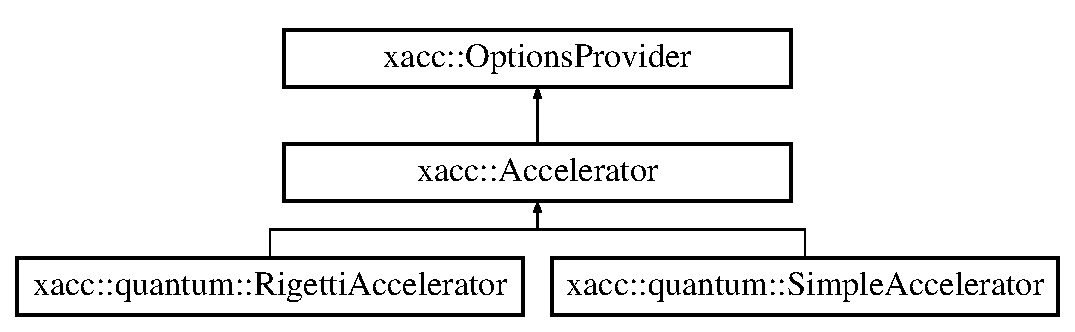
\includegraphics[height=2.679426cm]{a00011}
\end{center}
\end{figure}
\subsection*{Public Member Functions}
\begin{DoxyCompactItemize}
\item 
virtual void \hyperlink{a00011_a8cdc6f0c5a660013c29c07657a06303b}{initialize} ()=0
\item 
virtual Accelerator\+Type \hyperlink{a00011_aaffc3e4bb9880eb5041b1b58ee4c2665}{get\+Type} ()=0
\item 
virtual std\+::vector$<$ \hyperlink{a00051}{I\+R\+Transformation} $>$ \hyperlink{a00011_ad6e4a642dcb24e552675bcbeff1e1b04}{get\+I\+R\+Transformations} ()=0
\item 
virtual void \hyperlink{a00011_a89b3f3e6294f228abf03a410b0fb1674}{execute} (std\+::shared\+\_\+ptr$<$ \hyperlink{a00013}{Accelerator\+Buffer} $>$ buffer, const std\+::shared\+\_\+ptr$<$ \hyperlink{a00038}{Function} $>$ function)=0
\item 
virtual std\+::shared\+\_\+ptr$<$ \hyperlink{a00013}{Accelerator\+Buffer} $>$ \hyperlink{a00011_aab5046e8d83ab390302e0f49533e95fc}{create\+Buffer} (const std\+::string \&var\+Id)=0
\item 
virtual std\+::shared\+\_\+ptr$<$ \hyperlink{a00013}{Accelerator\+Buffer} $>$ \hyperlink{a00011_a064a2dbd58338364115c260267806945}{create\+Buffer} (const std\+::string \&var\+Id, const int size)=0
\item 
virtual std\+::shared\+\_\+ptr$<$ \hyperlink{a00013}{Accelerator\+Buffer} $>$ \hyperlink{a00011_ab3820be326e28a553fed1a824f4d41d0}{get\+Buffer} (const std\+::string \&varid)
\item 
virtual std\+::vector$<$ std\+::string $>$ \hyperlink{a00011_ae1463d7e405df89fa4af47e8922f4b82}{get\+Allocated\+Buffer\+Names} ()
\item 
virtual std\+::shared\+\_\+ptr$<$ \hyperlink{a00043}{Accelerator\+Graph} $>$ \hyperlink{a00011_adfed940ce1fa476b009344ddf5a4bbc3}{get\+Accelerator\+Connectivity} ()
\item 
virtual std\+::shared\+\_\+ptr$<$ options\+\_\+description $>$ \hyperlink{a00011_a98c9eda6b54367c75667ecfbbf167979}{get\+Options} ()
\item 
virtual \hyperlink{a00011_aed88ab0d71b765f0b0f512684ccd4b55}{$\sim$\+Accelerator} ()
\end{DoxyCompactItemize}
\subsection*{Protected Member Functions}
\begin{DoxyCompactItemize}
\item 
virtual bool \hyperlink{a00011_ae51584850faeec77299058383977ddeb}{is\+Valid\+Buffer\+Size} (const int N\+Bits)=0
\item 
void \hyperlink{a00011_ac3e781f42ec25e460174d4c41ea26b94}{store\+Buffer} (const std\+::string \&id, std\+::shared\+\_\+ptr$<$ \hyperlink{a00013}{Accelerator\+Buffer} $>$ b)
\end{DoxyCompactItemize}


\subsection{Detailed Description}
The \hyperlink{a00011}{Accelerator} class provides a high-\/level abstraction for X\+A\+CC\textquotesingle{}s interaction with attached post-\/exascale accelerators (quantum and neuromorphic processing units).

Derived Accelerators must provide a valid execute implementation that takes X\+A\+CC \hyperlink{a00050}{IR} and executes it on the attached hardware or simulator.

Derived Accelerators must provide a list of \hyperlink{a00051}{I\+R\+Transformation} instances that transform X\+A\+CC \hyperlink{a00050}{IR} to be amenable to execution on the hardware.

Derived Accelerators must provide implementations of create\+Buffer that provide a valid \hyperlink{a00013}{Accelerator\+Buffer} instance modeling the hardware memory or bits being computed on. Upon creating an \hyperlink{a00013}{Accelerator\+Buffer}, derived \hyperlink{a00011}{Accelerator} implementations must call the protected store\+Buffer method to store the \hyperlink{a00013}{Accelerator\+Buffer} for future reference by Compilers and clients of \hyperlink{a00011}{Accelerator}.

\begin{DoxyAuthor}{Author}
Alex Mc\+Caskey 
\end{DoxyAuthor}


\subsection{Constructor \& Destructor Documentation}
\index{xacc\+::\+Accelerator@{xacc\+::\+Accelerator}!````~Accelerator@{$\sim$\+Accelerator}}
\index{````~Accelerator@{$\sim$\+Accelerator}!xacc\+::\+Accelerator@{xacc\+::\+Accelerator}}
\subsubsection[{\texorpdfstring{$\sim$\+Accelerator()}{~Accelerator()}}]{\setlength{\rightskip}{0pt plus 5cm}virtual xacc\+::\+Accelerator\+::$\sim$\+Accelerator (
\begin{DoxyParamCaption}
{}
\end{DoxyParamCaption}
)\hspace{0.3cm}{\ttfamily [inline]}, {\ttfamily [virtual]}}\hypertarget{a00011_aed88ab0d71b765f0b0f512684ccd4b55}{}\label{a00011_aed88ab0d71b765f0b0f512684ccd4b55}
Destructor 

\subsection{Member Function Documentation}
\index{xacc\+::\+Accelerator@{xacc\+::\+Accelerator}!create\+Buffer@{create\+Buffer}}
\index{create\+Buffer@{create\+Buffer}!xacc\+::\+Accelerator@{xacc\+::\+Accelerator}}
\subsubsection[{\texorpdfstring{create\+Buffer(const std\+::string \&var\+Id)=0}{createBuffer(const std::string \&varId)=0}}]{\setlength{\rightskip}{0pt plus 5cm}virtual std\+::shared\+\_\+ptr$<${\bf Accelerator\+Buffer}$>$ xacc\+::\+Accelerator\+::create\+Buffer (
\begin{DoxyParamCaption}
\item[{const std\+::string \&}]{var\+Id}
\end{DoxyParamCaption}
)\hspace{0.3cm}{\ttfamily [pure virtual]}}\hypertarget{a00011_aab5046e8d83ab390302e0f49533e95fc}{}\label{a00011_aab5046e8d83ab390302e0f49533e95fc}
Create, store, and return an \hyperlink{a00013}{Accelerator\+Buffer} with the given variable id string. This method returns all available qubits for this \hyperlink{a00011}{Accelerator}. The string id serves as a unique identifier for future lookups and reuse of the \hyperlink{a00013}{Accelerator\+Buffer}.


\begin{DoxyParams}{Parameters}
{\em var\+Id} & The variable name of the created buffer \\
\hline
\end{DoxyParams}
\begin{DoxyReturn}{Returns}
buffer The buffer instance created. 
\end{DoxyReturn}


Implemented in \hyperlink{a00029_add60637a4b3c055e7f2ffa3bf8e320ac}{xacc\+::quantum\+::\+D\+W\+Accelerator}, \hyperlink{a00079_a46445d77d4b8ad2689571d0db6604380}{xacc\+::quantum\+::\+Simple\+Accelerator}, and \hyperlink{a00071_ada3ceb986e51ab5aa721f2a08e083cd6}{xacc\+::quantum\+::\+Rigetti\+Accelerator}.

\index{xacc\+::\+Accelerator@{xacc\+::\+Accelerator}!create\+Buffer@{create\+Buffer}}
\index{create\+Buffer@{create\+Buffer}!xacc\+::\+Accelerator@{xacc\+::\+Accelerator}}
\subsubsection[{\texorpdfstring{create\+Buffer(const std\+::string \&var\+Id, const int size)=0}{createBuffer(const std::string \&varId, const int size)=0}}]{\setlength{\rightskip}{0pt plus 5cm}virtual std\+::shared\+\_\+ptr$<${\bf Accelerator\+Buffer}$>$ xacc\+::\+Accelerator\+::create\+Buffer (
\begin{DoxyParamCaption}
\item[{const std\+::string \&}]{var\+Id, }
\item[{const int}]{size}
\end{DoxyParamCaption}
)\hspace{0.3cm}{\ttfamily [pure virtual]}}\hypertarget{a00011_a064a2dbd58338364115c260267806945}{}\label{a00011_a064a2dbd58338364115c260267806945}
Create, store, and return an \hyperlink{a00013}{Accelerator\+Buffer} with the given variable id string and of the given number of bits. The string id serves as a unique identifier for future lookups and reuse of the \hyperlink{a00013}{Accelerator\+Buffer}.


\begin{DoxyParams}{Parameters}
{\em var\+Id} & The variable name of the created buffer \\
\hline
{\em size} & The number of bits in the created buffer \\
\hline
\end{DoxyParams}
\begin{DoxyReturn}{Returns}
buffer The buffer instance created. 
\end{DoxyReturn}


Implemented in \hyperlink{a00029_a718d7cb51a35e694d960385e1ea2f99f}{xacc\+::quantum\+::\+D\+W\+Accelerator}, \hyperlink{a00071_a731551c94b1abef40d2cf032e8712df6}{xacc\+::quantum\+::\+Rigetti\+Accelerator}, and \hyperlink{a00079_adb9393692e9f484df241aa5d014030d1}{xacc\+::quantum\+::\+Simple\+Accelerator}.

\index{xacc\+::\+Accelerator@{xacc\+::\+Accelerator}!execute@{execute}}
\index{execute@{execute}!xacc\+::\+Accelerator@{xacc\+::\+Accelerator}}
\subsubsection[{\texorpdfstring{execute(std\+::shared\+\_\+ptr$<$ Accelerator\+Buffer $>$ buffer, const std\+::shared\+\_\+ptr$<$ Function $>$ function)=0}{execute(std::shared\_ptr< AcceleratorBuffer > buffer, const std::shared\_ptr< Function > function)=0}}]{\setlength{\rightskip}{0pt plus 5cm}virtual void xacc\+::\+Accelerator\+::execute (
\begin{DoxyParamCaption}
\item[{std\+::shared\+\_\+ptr$<$ {\bf Accelerator\+Buffer} $>$}]{buffer, }
\item[{const std\+::shared\+\_\+ptr$<$ {\bf Function} $>$}]{function}
\end{DoxyParamCaption}
)\hspace{0.3cm}{\ttfamily [pure virtual]}}\hypertarget{a00011_a89b3f3e6294f228abf03a410b0fb1674}{}\label{a00011_a89b3f3e6294f228abf03a410b0fb1674}
Execute the provided X\+A\+CC \hyperlink{a00050}{IR} \hyperlink{a00038}{Function} on the provided \hyperlink{a00013}{Accelerator\+Buffer}.


\begin{DoxyParams}{Parameters}
{\em buffer} & The buffer of bits this \hyperlink{a00011}{Accelerator} should operate on. \\
\hline
{\em function} & The kernel to execute. \\
\hline
\end{DoxyParams}
\index{xacc\+::\+Accelerator@{xacc\+::\+Accelerator}!get\+Accelerator\+Connectivity@{get\+Accelerator\+Connectivity}}
\index{get\+Accelerator\+Connectivity@{get\+Accelerator\+Connectivity}!xacc\+::\+Accelerator@{xacc\+::\+Accelerator}}
\subsubsection[{\texorpdfstring{get\+Accelerator\+Connectivity()}{getAcceleratorConnectivity()}}]{\setlength{\rightskip}{0pt plus 5cm}virtual std\+::shared\+\_\+ptr$<${\bf Accelerator\+Graph}$>$ xacc\+::\+Accelerator\+::get\+Accelerator\+Connectivity (
\begin{DoxyParamCaption}
{}
\end{DoxyParamCaption}
)\hspace{0.3cm}{\ttfamily [inline]}, {\ttfamily [virtual]}}\hypertarget{a00011_adfed940ce1fa476b009344ddf5a4bbc3}{}\label{a00011_adfed940ce1fa476b009344ddf5a4bbc3}
Return the graph structure for this \hyperlink{a00011}{Accelerator}.

\begin{DoxyReturn}{Returns}
connectivity\+Graph The graph structure of this \hyperlink{a00011}{Accelerator} 
\end{DoxyReturn}


Reimplemented in \hyperlink{a00029_a006afa60749790681fc76beddc254926}{xacc\+::quantum\+::\+D\+W\+Accelerator}.

\index{xacc\+::\+Accelerator@{xacc\+::\+Accelerator}!get\+Allocated\+Buffer\+Names@{get\+Allocated\+Buffer\+Names}}
\index{get\+Allocated\+Buffer\+Names@{get\+Allocated\+Buffer\+Names}!xacc\+::\+Accelerator@{xacc\+::\+Accelerator}}
\subsubsection[{\texorpdfstring{get\+Allocated\+Buffer\+Names()}{getAllocatedBufferNames()}}]{\setlength{\rightskip}{0pt plus 5cm}virtual std\+::vector$<$std\+::string$>$ xacc\+::\+Accelerator\+::get\+Allocated\+Buffer\+Names (
\begin{DoxyParamCaption}
{}
\end{DoxyParamCaption}
)\hspace{0.3cm}{\ttfamily [inline]}, {\ttfamily [virtual]}}\hypertarget{a00011_ae1463d7e405df89fa4af47e8922f4b82}{}\label{a00011_ae1463d7e405df89fa4af47e8922f4b82}
Return all allocated \hyperlink{a00013}{Accelerator\+Buffer} variable names.

\begin{DoxyReturn}{Returns}
var\+Names The buffer variable names 
\end{DoxyReturn}
\index{xacc\+::\+Accelerator@{xacc\+::\+Accelerator}!get\+Buffer@{get\+Buffer}}
\index{get\+Buffer@{get\+Buffer}!xacc\+::\+Accelerator@{xacc\+::\+Accelerator}}
\subsubsection[{\texorpdfstring{get\+Buffer(const std\+::string \&varid)}{getBuffer(const std::string \&varid)}}]{\setlength{\rightskip}{0pt plus 5cm}virtual std\+::shared\+\_\+ptr$<${\bf Accelerator\+Buffer}$>$ xacc\+::\+Accelerator\+::get\+Buffer (
\begin{DoxyParamCaption}
\item[{const std\+::string \&}]{varid}
\end{DoxyParamCaption}
)\hspace{0.3cm}{\ttfamily [inline]}, {\ttfamily [virtual]}}\hypertarget{a00011_ab3820be326e28a553fed1a824f4d41d0}{}\label{a00011_ab3820be326e28a553fed1a824f4d41d0}
Return the stored \hyperlink{a00013}{Accelerator\+Buffer} with the provided string id.


\begin{DoxyParams}{Parameters}
{\em varid} & The variable name of the created buffer \\
\hline
\end{DoxyParams}
\begin{DoxyReturn}{Returns}
buffer The buffer with given varid. 
\end{DoxyReturn}
\index{xacc\+::\+Accelerator@{xacc\+::\+Accelerator}!get\+I\+R\+Transformations@{get\+I\+R\+Transformations}}
\index{get\+I\+R\+Transformations@{get\+I\+R\+Transformations}!xacc\+::\+Accelerator@{xacc\+::\+Accelerator}}
\subsubsection[{\texorpdfstring{get\+I\+R\+Transformations()=0}{getIRTransformations()=0}}]{\setlength{\rightskip}{0pt plus 5cm}virtual std\+::vector$<${\bf I\+R\+Transformation}$>$ xacc\+::\+Accelerator\+::get\+I\+R\+Transformations (
\begin{DoxyParamCaption}
{}
\end{DoxyParamCaption}
)\hspace{0.3cm}{\ttfamily [pure virtual]}}\hypertarget{a00011_ad6e4a642dcb24e552675bcbeff1e1b04}{}\label{a00011_ad6e4a642dcb24e552675bcbeff1e1b04}
Return any \hyperlink{a00050}{IR} Transformations that must be applied to ensure the compiled \hyperlink{a00050}{IR} is amenable to execution on this \hyperlink{a00011}{Accelerator}.

\begin{DoxyReturn}{Returns}
transformations The \hyperlink{a00050}{IR} transformations this \hyperlink{a00011}{Accelerator} exposes 
\end{DoxyReturn}


Implemented in \hyperlink{a00029_a89da20bd079a22d6581ea2da2293b973}{xacc\+::quantum\+::\+D\+W\+Accelerator}, \hyperlink{a00071_a443683a1dfb000603c640b2ee303cf66}{xacc\+::quantum\+::\+Rigetti\+Accelerator}, and \hyperlink{a00079_afc49c9e7973ba6c6ff9761c36198323d}{xacc\+::quantum\+::\+Simple\+Accelerator}.

\index{xacc\+::\+Accelerator@{xacc\+::\+Accelerator}!get\+Options@{get\+Options}}
\index{get\+Options@{get\+Options}!xacc\+::\+Accelerator@{xacc\+::\+Accelerator}}
\subsubsection[{\texorpdfstring{get\+Options()}{getOptions()}}]{\setlength{\rightskip}{0pt plus 5cm}virtual std\+::shared\+\_\+ptr$<$options\+\_\+description$>$ xacc\+::\+Accelerator\+::get\+Options (
\begin{DoxyParamCaption}
{}
\end{DoxyParamCaption}
)\hspace{0.3cm}{\ttfamily [inline]}, {\ttfamily [virtual]}}\hypertarget{a00011_a98c9eda6b54367c75667ecfbbf167979}{}\label{a00011_a98c9eda6b54367c75667ecfbbf167979}
Return an empty options\+\_\+description, this is for subclasses to implement. 

Implements \hyperlink{a00056_a6d150954f852109bfe2c1ae90222926f}{xacc\+::\+Options\+Provider}.



Reimplemented in \hyperlink{a00029_a09926db9f99706307ae6ce5b56845bca}{xacc\+::quantum\+::\+D\+W\+Accelerator}, and \hyperlink{a00071_a9ee9e62aecbccf193894ca3388676f9f}{xacc\+::quantum\+::\+Rigetti\+Accelerator}.

\index{xacc\+::\+Accelerator@{xacc\+::\+Accelerator}!get\+Type@{get\+Type}}
\index{get\+Type@{get\+Type}!xacc\+::\+Accelerator@{xacc\+::\+Accelerator}}
\subsubsection[{\texorpdfstring{get\+Type()=0}{getType()=0}}]{\setlength{\rightskip}{0pt plus 5cm}virtual Accelerator\+Type xacc\+::\+Accelerator\+::get\+Type (
\begin{DoxyParamCaption}
{}
\end{DoxyParamCaption}
)\hspace{0.3cm}{\ttfamily [pure virtual]}}\hypertarget{a00011_aaffc3e4bb9880eb5041b1b58ee4c2665}{}\label{a00011_aaffc3e4bb9880eb5041b1b58ee4c2665}
Return the type of this \hyperlink{a00011}{Accelerator}.

\begin{DoxyReturn}{Returns}
type The \hyperlink{a00011}{Accelerator} type -\/ Gate or A\+QC Q\+PU, or N\+PU 
\end{DoxyReturn}


Implemented in \hyperlink{a00029_abe50e427b4bec0460cc238405cb569f9}{xacc\+::quantum\+::\+D\+W\+Accelerator}, \hyperlink{a00071_aab0d4674da5273d55407b9ab77cde890}{xacc\+::quantum\+::\+Rigetti\+Accelerator}, and \hyperlink{a00079_ad76eeb0bbd7de21aad5bd20d20970a98}{xacc\+::quantum\+::\+Simple\+Accelerator}.

\index{xacc\+::\+Accelerator@{xacc\+::\+Accelerator}!initialize@{initialize}}
\index{initialize@{initialize}!xacc\+::\+Accelerator@{xacc\+::\+Accelerator}}
\subsubsection[{\texorpdfstring{initialize()=0}{initialize()=0}}]{\setlength{\rightskip}{0pt plus 5cm}virtual void xacc\+::\+Accelerator\+::initialize (
\begin{DoxyParamCaption}
{}
\end{DoxyParamCaption}
)\hspace{0.3cm}{\ttfamily [pure virtual]}}\hypertarget{a00011_a8cdc6f0c5a660013c29c07657a06303b}{}\label{a00011_a8cdc6f0c5a660013c29c07657a06303b}
Initialize this \hyperlink{a00011}{Accelerator}. This method is called by the X\+A\+CC framework after an \hyperlink{a00011}{Accelerator} has been requested and created. Perform any work you need done before execution here. 

Implemented in \hyperlink{a00029_acaefd5747409f31cf5c3e42d98475ce2}{xacc\+::quantum\+::\+D\+W\+Accelerator}, \hyperlink{a00071_ab8b6af9bb9dcb110201e9ee5cac74b4f}{xacc\+::quantum\+::\+Rigetti\+Accelerator}, and \hyperlink{a00079_a392e3b30523f5f681127e7e98887108c}{xacc\+::quantum\+::\+Simple\+Accelerator}.

\index{xacc\+::\+Accelerator@{xacc\+::\+Accelerator}!is\+Valid\+Buffer\+Size@{is\+Valid\+Buffer\+Size}}
\index{is\+Valid\+Buffer\+Size@{is\+Valid\+Buffer\+Size}!xacc\+::\+Accelerator@{xacc\+::\+Accelerator}}
\subsubsection[{\texorpdfstring{is\+Valid\+Buffer\+Size(const int N\+Bits)=0}{isValidBufferSize(const int NBits)=0}}]{\setlength{\rightskip}{0pt plus 5cm}virtual bool xacc\+::\+Accelerator\+::is\+Valid\+Buffer\+Size (
\begin{DoxyParamCaption}
\item[{const int}]{N\+Bits}
\end{DoxyParamCaption}
)\hspace{0.3cm}{\ttfamily [protected]}, {\ttfamily [pure virtual]}}\hypertarget{a00011_ae51584850faeec77299058383977ddeb}{}\label{a00011_ae51584850faeec77299058383977ddeb}
Return true if this \hyperlink{a00011}{Accelerator} can allocated N\+Bits number of bits. This is meant to be implemented and used by subclasses.


\begin{DoxyParams}{Parameters}
{\em N\+Bits} & The number of bits to allocate \\
\hline
\end{DoxyParams}
\begin{DoxyReturn}{Returns}
valid True if size is valid. 
\end{DoxyReturn}


Implemented in \hyperlink{a00029_a4c2ee30212a919d8ddf7f9555df25195}{xacc\+::quantum\+::\+D\+W\+Accelerator}, \hyperlink{a00079_a60b9db2d6aed235857c45413a070338e}{xacc\+::quantum\+::\+Simple\+Accelerator}, and \hyperlink{a00071_a61352c07062597aad2393fbeed4cc025}{xacc\+::quantum\+::\+Rigetti\+Accelerator}.

\index{xacc\+::\+Accelerator@{xacc\+::\+Accelerator}!store\+Buffer@{store\+Buffer}}
\index{store\+Buffer@{store\+Buffer}!xacc\+::\+Accelerator@{xacc\+::\+Accelerator}}
\subsubsection[{\texorpdfstring{store\+Buffer(const std\+::string \&id, std\+::shared\+\_\+ptr$<$ Accelerator\+Buffer $>$ b)}{storeBuffer(const std::string \&id, std::shared\_ptr< AcceleratorBuffer > b)}}]{\setlength{\rightskip}{0pt plus 5cm}void xacc\+::\+Accelerator\+::store\+Buffer (
\begin{DoxyParamCaption}
\item[{const std\+::string \&}]{id, }
\item[{std\+::shared\+\_\+ptr$<$ {\bf Accelerator\+Buffer} $>$}]{b}
\end{DoxyParamCaption}
)\hspace{0.3cm}{\ttfamily [inline]}, {\ttfamily [protected]}}\hypertarget{a00011_ac3e781f42ec25e460174d4c41ea26b94}{}\label{a00011_ac3e781f42ec25e460174d4c41ea26b94}
This protected method is to be used by derived Accelerators to store any created \hyperlink{a00013}{Accelerator\+Buffer}.


\begin{DoxyParams}{Parameters}
{\em id} & The variable name of the buffer to store \\
\hline
{\em b} & The buffer to store \\
\hline
\end{DoxyParams}


The documentation for this class was generated from the following file\+:\begin{DoxyCompactItemize}
\item 
Accelerator.\+hpp\end{DoxyCompactItemize}

\chapter{2016-\/10-\/30-\/parsers}
\label{a00012}
\hypertarget{a00012}{}
\hypertarget{a00012}{}\section{xacc\+:\+:Accelerator\+Bit Class Reference}
\label{a00012}\index{xacc\+::\+Accelerator\+Bit@{xacc\+::\+Accelerator\+Bit}}


{\ttfamily \#include $<$Accelerator\+Buffer.\+hpp$>$}

\subsection*{Public Member Functions}
\begin{DoxyCompactItemize}
\item 
\hyperlink{a00012_a9a124c230c5cabeab53bac0820c0221a}{Accelerator\+Bit} ()
\item 
void \hyperlink{a00012_aa63a24980e831b9325a36836ab1c5495}{update} (int zero\+Or\+One)
\item 
Accelerator\+Bit\+State \hyperlink{a00012_a4a8dcc4fa02a5619f583961460c77057}{get\+State} ()
\end{DoxyCompactItemize}
\subsection*{Protected Attributes}
\begin{DoxyCompactItemize}
\item 
Accelerator\+Bit\+State \hyperlink{a00012_a4632123ac31aeed0dc97c65f8c792a85}{state}
\end{DoxyCompactItemize}


\subsection{Detailed Description}
The \hyperlink{a00012}{Accelerator\+Bit} wraps an Accelerator\+Bit\+Sate and provides a mechanism for updating that state.

\begin{DoxyAuthor}{Author}
Alex Mc\+Caskey 
\end{DoxyAuthor}


\subsection{Constructor \& Destructor Documentation}
\index{xacc\+::\+Accelerator\+Bit@{xacc\+::\+Accelerator\+Bit}!Accelerator\+Bit@{Accelerator\+Bit}}
\index{Accelerator\+Bit@{Accelerator\+Bit}!xacc\+::\+Accelerator\+Bit@{xacc\+::\+Accelerator\+Bit}}
\subsubsection[{\texorpdfstring{Accelerator\+Bit()}{AcceleratorBit()}}]{\setlength{\rightskip}{0pt plus 5cm}xacc\+::\+Accelerator\+Bit\+::\+Accelerator\+Bit (
\begin{DoxyParamCaption}
{}
\end{DoxyParamCaption}
)\hspace{0.3cm}{\ttfamily [inline]}}\hypertarget{a00012_a9a124c230c5cabeab53bac0820c0221a}{}\label{a00012_a9a124c230c5cabeab53bac0820c0221a}
The constructor, all bits are initialized to unknown state 

\subsection{Member Function Documentation}
\index{xacc\+::\+Accelerator\+Bit@{xacc\+::\+Accelerator\+Bit}!get\+State@{get\+State}}
\index{get\+State@{get\+State}!xacc\+::\+Accelerator\+Bit@{xacc\+::\+Accelerator\+Bit}}
\subsubsection[{\texorpdfstring{get\+State()}{getState()}}]{\setlength{\rightskip}{0pt plus 5cm}Accelerator\+Bit\+State xacc\+::\+Accelerator\+Bit\+::get\+State (
\begin{DoxyParamCaption}
{}
\end{DoxyParamCaption}
)\hspace{0.3cm}{\ttfamily [inline]}}\hypertarget{a00012_a4a8dcc4fa02a5619f583961460c77057}{}\label{a00012_a4a8dcc4fa02a5619f583961460c77057}
Return the value of this state \index{xacc\+::\+Accelerator\+Bit@{xacc\+::\+Accelerator\+Bit}!update@{update}}
\index{update@{update}!xacc\+::\+Accelerator\+Bit@{xacc\+::\+Accelerator\+Bit}}
\subsubsection[{\texorpdfstring{update(int zero\+Or\+One)}{update(int zeroOrOne)}}]{\setlength{\rightskip}{0pt plus 5cm}void xacc\+::\+Accelerator\+Bit\+::update (
\begin{DoxyParamCaption}
\item[{int}]{zero\+Or\+One}
\end{DoxyParamCaption}
)\hspace{0.3cm}{\ttfamily [inline]}}\hypertarget{a00012_aa63a24980e831b9325a36836ab1c5495}{}\label{a00012_aa63a24980e831b9325a36836ab1c5495}
Update the Bit state to a one or zero 

\subsection{Member Data Documentation}
\index{xacc\+::\+Accelerator\+Bit@{xacc\+::\+Accelerator\+Bit}!state@{state}}
\index{state@{state}!xacc\+::\+Accelerator\+Bit@{xacc\+::\+Accelerator\+Bit}}
\subsubsection[{\texorpdfstring{state}{state}}]{\setlength{\rightskip}{0pt plus 5cm}Accelerator\+Bit\+State xacc\+::\+Accelerator\+Bit\+::state\hspace{0.3cm}{\ttfamily [protected]}}\hypertarget{a00012_a4632123ac31aeed0dc97c65f8c792a85}{}\label{a00012_a4632123ac31aeed0dc97c65f8c792a85}
The bit state 

The documentation for this class was generated from the following file\+:\begin{DoxyCompactItemize}
\item 
Accelerator\+Buffer.\+hpp\end{DoxyCompactItemize}

\chapter{2016-\/10-\/30-\/tests}
\label{a00013}
\hypertarget{a00013}{}
\hypertarget{a00013}{}\section{xacc\+:\+:Accelerator\+Buffer Class Reference}
\label{a00013}\index{xacc\+::\+Accelerator\+Buffer@{xacc\+::\+Accelerator\+Buffer}}


{\ttfamily \#include $<$Accelerator\+Buffer.\+hpp$>$}

Inheritance diagram for xacc\+:\+:Accelerator\+Buffer\+:\begin{figure}[H]
\begin{center}
\leavevmode
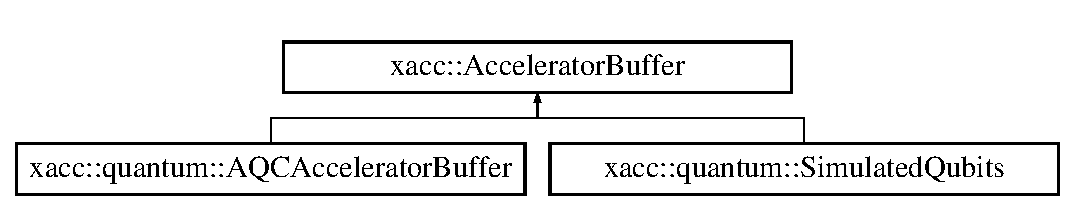
\includegraphics[height=2.000000cm]{a00013}
\end{center}
\end{figure}
\subsection*{Public Member Functions}
\begin{DoxyCompactItemize}
\item 
\hyperlink{a00013_ab606d8af942120d60b51a4fffcd75c98}{Accelerator\+Buffer} (const std\+::string \&str, const int N)
\item 
{\footnotesize template$<$typename... Indices$>$ }\\{\bfseries Accelerator\+Buffer} (const std\+::string \&str, int first\+Index, Indices...\+indices)\hypertarget{a00013_ac550d89390562095c56aa1b14ae85001}{}\label{a00013_ac550d89390562095c56aa1b14ae85001}

\item 
int {\bfseries size} ()\hypertarget{a00013_aa2a3101c2e3ae3550172bf49f9587f3b}{}\label{a00013_aa2a3101c2e3ae3550172bf49f9587f3b}

\item 
std\+::string {\bfseries name} ()\hypertarget{a00013_ad5b646e9efc21b6d0bcc22cd6f649c22}{}\label{a00013_ad5b646e9efc21b6d0bcc22cd6f649c22}

\item 
void {\bfseries reset\+Buffer} ()\hypertarget{a00013_aa6d6e9cfee6170333c1f03507345743f}{}\label{a00013_aa6d6e9cfee6170333c1f03507345743f}

\item 
void {\bfseries update\+Bit} (const int idx, int zero\+Or\+One)\hypertarget{a00013_a4bc0edbe9aa0d463f67ddcc38265066f}{}\label{a00013_a4bc0edbe9aa0d463f67ddcc38265066f}

\item 
void {\bfseries append\+Measurement} (const boost\+::dynamic\+\_\+bitset$<$$>$ \&measurement)\hypertarget{a00013_ac161c4f984f774d08197871094aabc67}{}\label{a00013_ac161c4f984f774d08197871094aabc67}

\item 
double {\bfseries get\+Average} () const \hypertarget{a00013_a97cf3cc4e1aaa8ac3cee7817860f77c1}{}\label{a00013_a97cf3cc4e1aaa8ac3cee7817860f77c1}

\item 
Accelerator\+Bit\+State {\bfseries get\+Accelerator\+Bit\+State} (const int idx)\hypertarget{a00013_aba6ef359f3117faa98f0eb8da90d909e}{}\label{a00013_aba6ef359f3117faa98f0eb8da90d909e}

\item 
virtual void {\bfseries print} ()\hypertarget{a00013_add0835e188f0eda4f1b68a28ddc79786}{}\label{a00013_add0835e188f0eda4f1b68a28ddc79786}

\item 
virtual void {\bfseries print} (std\+::ostream \&stream)\hypertarget{a00013_a7c59462451223772b41ef232b06a7dfa}{}\label{a00013_a7c59462451223772b41ef232b06a7dfa}

\end{DoxyCompactItemize}
\subsection*{Protected Attributes}
\begin{DoxyCompactItemize}
\item 
std\+::vector$<$ boost\+::dynamic\+\_\+bitset$<$$>$ $>$ {\bfseries measurements}\hypertarget{a00013_a5464b23a964985df2547f657877c9ea5}{}\label{a00013_a5464b23a964985df2547f657877c9ea5}

\item 
std\+::string {\bfseries buffer\+Id}\hypertarget{a00013_a3198e034d07d9b77b62da03e6592a221}{}\label{a00013_a3198e034d07d9b77b62da03e6592a221}

\item 
std\+::vector$<$ \hyperlink{a00012}{Accelerator\+Bit} $>$ {\bfseries bits}\hypertarget{a00013_ab6dbb8c22f8adc6aba34b00a84066854}{}\label{a00013_ab6dbb8c22f8adc6aba34b00a84066854}

\end{DoxyCompactItemize}


\subsection{Detailed Description}
The \hyperlink{a00013}{Accelerator\+Buffer} models an allocated buffer of bits that are operated on by a kernel. As such, the \hyperlink{a00013}{Accelerator\+Buffer}\textquotesingle{}s primary role is to store \hyperlink{a00011}{Accelerator} execution results.

\begin{DoxyAuthor}{Author}
Alex Mc\+Caskey 
\end{DoxyAuthor}


\subsection{Constructor \& Destructor Documentation}
\index{xacc\+::\+Accelerator\+Buffer@{xacc\+::\+Accelerator\+Buffer}!Accelerator\+Buffer@{Accelerator\+Buffer}}
\index{Accelerator\+Buffer@{Accelerator\+Buffer}!xacc\+::\+Accelerator\+Buffer@{xacc\+::\+Accelerator\+Buffer}}
\subsubsection[{\texorpdfstring{Accelerator\+Buffer(const std\+::string \&str, const int N)}{AcceleratorBuffer(const std::string \&str, const int N)}}]{\setlength{\rightskip}{0pt plus 5cm}xacc\+::\+Accelerator\+Buffer\+::\+Accelerator\+Buffer (
\begin{DoxyParamCaption}
\item[{const std\+::string \&}]{str, }
\item[{const int}]{N}
\end{DoxyParamCaption}
)\hspace{0.3cm}{\ttfamily [inline]}}\hypertarget{a00013_ab606d8af942120d60b51a4fffcd75c98}{}\label{a00013_ab606d8af942120d60b51a4fffcd75c98}
The Constructor 

The documentation for this class was generated from the following file\+:\begin{DoxyCompactItemize}
\item 
Accelerator\+Buffer.\+hpp\end{DoxyCompactItemize}

\chapter{2016-\/11-\/06-\/astrophysical-\/reactions}
\label{a00014}
\hypertarget{a00014}{}
\hypertarget{a00014}{}\section{xacc\+:\+:quantum\+:\+:All\+Gate\+Visitor Class Reference}
\label{a00014}\index{xacc\+::quantum\+::\+All\+Gate\+Visitor@{xacc\+::quantum\+::\+All\+Gate\+Visitor}}


{\ttfamily \#include $<$All\+Gate\+Visitor.\+hpp$>$}

Inheritance diagram for xacc\+:\+:quantum\+:\+:All\+Gate\+Visitor\+:\begin{figure}[H]
\begin{center}
\leavevmode
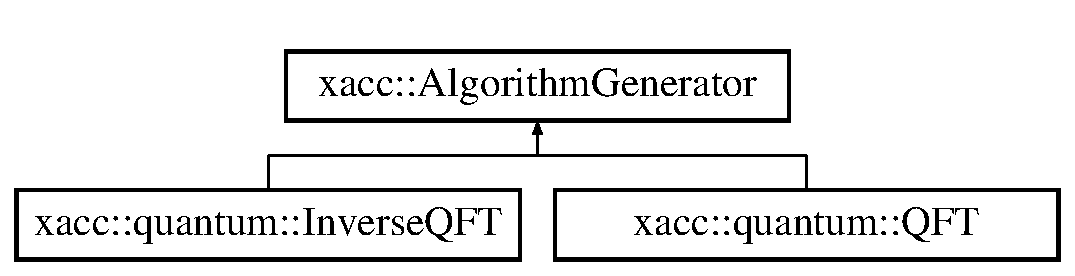
\includegraphics[height=9.201878cm]{a00014}
\end{center}
\end{figure}
\subsection*{Additional Inherited Members}


\subsection{Detailed Description}
F\+I\+X\+ME write this 

The documentation for this class was generated from the following file\+:\begin{DoxyCompactItemize}
\item 
All\+Gate\+Visitor.\+hpp\end{DoxyCompactItemize}

\chapter{2016-\/11-\/12-\/astrophysics-\/reactions-\/ascii-\/format}
\label{a00015}
\hypertarget{a00015}{}


 layout\+: post title\+: Astrophysics Reactions \hyperlink{a00038}{A\+S\+C\+II} File Format permalink\+: /science/astrophysics/reactions-\/ascii-\/format \subsection*{category\+: science }

Simulations of thermonuclear networks in astrophysics require lists of reactions that describe how the species evolve over time. Fire supports a legacy \hyperlink{a00038}{A\+S\+C\+II} format with a 8-\/line specification for a reaction. Each entry in each line is separated by a space. See \hyperlink{a00678_source}{Reaction.\+h} for full details on each required value.

The first line for each reaction contains\+:


\begin{DoxyItemize}
\item Name/\+Label -\/ A string of the form \char`\"{}he4+he4+he4-\/-\/$>$c12\char`\"{} that describes the reaction.
\item Reaction Group Class -\/ an integer
\item Reaction Group Index -\/ an integer
\item R\+E\+A\+C\+L\+IB Class -\/ an integer
\item Number of reacting species -\/ an integer
\item Number of resulting products -\/ an integer
\item Electron capture flag -\/ a bool
\item Reverse reaction flag -\/ a bool
\item Statistical factor -\/ a double
\item Energy release -\/ a double
\end{DoxyItemize}

The second line contains the seven rate coefficients from the R\+E\+A\+C\+L\+IB library, all doubles. The third line contains the array of atomic numbers for the reactants in this reaction, which are integers. The fourth, fifth, and sixth lines are also integers for the reactant neutron number and product atomic and neutron numbers. Each of these four lines has one integer for each reactant and product in the system, but with no more than four entries per line. (See example below for more details.)

The seventh and eighth lines contain quantities that are used for {\itshape Partial Equilibrium} approximations. Each line contains up to three integers.


\begin{DoxyCode}
1 he4+he4+he4-->c12 3 0 8 3 1 0 0 0.16666667 7.27500
2 -24.99350000 -4.29702000 -6.69304000 15.59030000 -1.57387000 0.17058800 -9.02800000
3 2 2 2 // Since numReactants = 3 and he4 has Z=2, there are three values on this line equal to 2.
4 2 2 2 // Same, but for he4's neutron number
5 6 // There is only one product and Z=6 for C12.
6 6 // N=6 for C12
7 0 0 0 
8 1 
9 ne20-->he4+o16 2 3 2 1 2 0 1 1.00000000 -4.73400
10 109.31000000 -72.75840000 293.66400000 -384.97400000 20.23800000 -1.00379000 201.19300000
11 10 // Z for ne20
12 10 // N for ne20
13 2 8 // Z for he4 and o16
14 2 8 // N for he4 and o16
15 3 
16 0 2 
\end{DoxyCode}
 
\chapter{2016-\/11-\/12-\/astrophysics-\/species-\/ascii-\/format}
\label{a00016}
\hypertarget{a00016}{}
\hypertarget{a00016}{}\section{xacc\+:\+:Base\+Instruction\+Visitor Class Reference}
\label{a00016}\index{xacc\+::\+Base\+Instruction\+Visitor@{xacc\+::\+Base\+Instruction\+Visitor}}


{\ttfamily \#include $<$Instruction\+Visitor.\+hpp$>$}

Inheritance diagram for xacc\+:\+:Base\+Instruction\+Visitor\+:\begin{figure}[H]
\begin{center}
\leavevmode
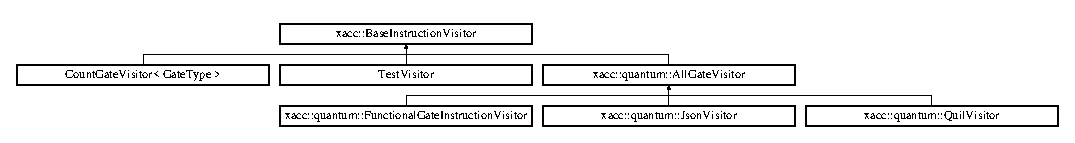
\includegraphics[height=1.478873cm]{a00016}
\end{center}
\end{figure}
\subsection*{Public Member Functions}
\begin{DoxyCompactItemize}
\item 
virtual \hyperlink{a00016_aa6f5104f5868fe1eca9be4dc4036eba4}{$\sim$\+Base\+Instruction\+Visitor} ()
\end{DoxyCompactItemize}


\subsection{Detailed Description}
The \hyperlink{a00016}{Base\+Instruction\+Visitor} is a base class for all classes that are \hyperlink{a00037}{Instruction} visitors. It basically provides a means for passing instruction visitor handles in a polymorphic manner. 

\subsection{Constructor \& Destructor Documentation}
\index{xacc\+::\+Base\+Instruction\+Visitor@{xacc\+::\+Base\+Instruction\+Visitor}!````~Base\+Instruction\+Visitor@{$\sim$\+Base\+Instruction\+Visitor}}
\index{````~Base\+Instruction\+Visitor@{$\sim$\+Base\+Instruction\+Visitor}!xacc\+::\+Base\+Instruction\+Visitor@{xacc\+::\+Base\+Instruction\+Visitor}}
\subsubsection[{\texorpdfstring{$\sim$\+Base\+Instruction\+Visitor()}{~BaseInstructionVisitor()}}]{\setlength{\rightskip}{0pt plus 5cm}virtual xacc\+::\+Base\+Instruction\+Visitor\+::$\sim$\+Base\+Instruction\+Visitor (
\begin{DoxyParamCaption}
{}
\end{DoxyParamCaption}
)\hspace{0.3cm}{\ttfamily [inline]}, {\ttfamily [virtual]}}\hypertarget{a00016_aa6f5104f5868fe1eca9be4dc4036eba4}{}\label{a00016_aa6f5104f5868fe1eca9be4dc4036eba4}
The destructor 

The documentation for this class was generated from the following file\+:\begin{DoxyCompactItemize}
\item 
Instruction\+Visitor.\+hpp\end{DoxyCompactItemize}

\chapter{2016-\/11-\/13-\/\+Notes-\/\+On-\/\+Getting-\/\+Eclipse-\/\+To-\/\+Work}
\label{a00017}
\hypertarget{a00017}{}
\hypertarget{a00017}{}\section{xacc\+:\+:Accelerator Class Reference}
\label{a00017}\index{xacc\+::\+Accelerator@{xacc\+::\+Accelerator}}


{\ttfamily \#include $<$Accelerator.\+hpp$>$}

Inheritance diagram for xacc\+:\+:Accelerator\+:\begin{figure}[H]
\begin{center}
\leavevmode
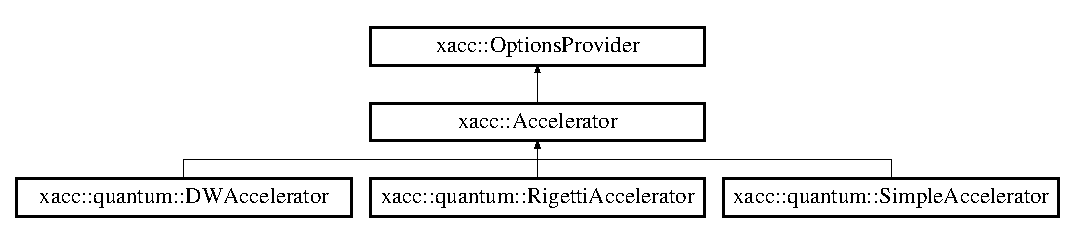
\includegraphics[height=2.679426cm]{a00017}
\end{center}
\end{figure}
\subsection*{Public Member Functions}
\begin{DoxyCompactItemize}
\item 
virtual void \hyperlink{a00017_a8cdc6f0c5a660013c29c07657a06303b}{initialize} ()=0
\item 
virtual Accelerator\+Type \hyperlink{a00017_aaffc3e4bb9880eb5041b1b58ee4c2665}{get\+Type} ()=0
\item 
virtual std\+::vector$<$ \hyperlink{a00078}{I\+R\+Transformation} $>$ \hyperlink{a00017_ad6e4a642dcb24e552675bcbeff1e1b04}{get\+I\+R\+Transformations} ()=0
\item 
virtual void \hyperlink{a00017_a89b3f3e6294f228abf03a410b0fb1674}{execute} (std\+::shared\+\_\+ptr$<$ \hyperlink{a00019}{Accelerator\+Buffer} $>$ buffer, const std\+::shared\+\_\+ptr$<$ \hyperlink{a00059}{Function} $>$ function)=0
\item 
virtual std\+::shared\+\_\+ptr$<$ \hyperlink{a00019}{Accelerator\+Buffer} $>$ \hyperlink{a00017_aab5046e8d83ab390302e0f49533e95fc}{create\+Buffer} (const std\+::string \&var\+Id)=0
\item 
virtual std\+::shared\+\_\+ptr$<$ \hyperlink{a00019}{Accelerator\+Buffer} $>$ \hyperlink{a00017_a064a2dbd58338364115c260267806945}{create\+Buffer} (const std\+::string \&var\+Id, const int size)=0
\item 
virtual std\+::shared\+\_\+ptr$<$ \hyperlink{a00019}{Accelerator\+Buffer} $>$ \hyperlink{a00017_ab3820be326e28a553fed1a824f4d41d0}{get\+Buffer} (const std\+::string \&varid)
\item 
virtual std\+::vector$<$ std\+::string $>$ \hyperlink{a00017_ae1463d7e405df89fa4af47e8922f4b82}{get\+Allocated\+Buffer\+Names} ()
\item 
virtual std\+::shared\+\_\+ptr$<$ \hyperlink{a00064}{Accelerator\+Graph} $>$ \hyperlink{a00017_adfed940ce1fa476b009344ddf5a4bbc3}{get\+Accelerator\+Connectivity} ()
\item 
virtual std\+::shared\+\_\+ptr$<$ options\+\_\+description $>$ \hyperlink{a00017_a98c9eda6b54367c75667ecfbbf167979}{get\+Options} ()
\item 
virtual \hyperlink{a00017_aed88ab0d71b765f0b0f512684ccd4b55}{$\sim$\+Accelerator} ()
\end{DoxyCompactItemize}
\subsection*{Protected Member Functions}
\begin{DoxyCompactItemize}
\item 
virtual bool \hyperlink{a00017_ae51584850faeec77299058383977ddeb}{is\+Valid\+Buffer\+Size} (const int N\+Bits)=0
\item 
void \hyperlink{a00017_ac3e781f42ec25e460174d4c41ea26b94}{store\+Buffer} (const std\+::string \&id, std\+::shared\+\_\+ptr$<$ \hyperlink{a00019}{Accelerator\+Buffer} $>$ b)
\end{DoxyCompactItemize}


\subsection{Detailed Description}
The \hyperlink{a00017}{Accelerator} class provides a high-\/level abstraction for X\+A\+CC\textquotesingle{}s interaction with attached post-\/exascale accelerators (quantum and neuromorphic processing units).

Derived Accelerators must provide a valid execute implementation that takes X\+A\+CC \hyperlink{a00077}{IR} and executes it on the attached hardware or simulator.

Derived Accelerators must provide a list of \hyperlink{a00078}{I\+R\+Transformation} instances that transform X\+A\+CC \hyperlink{a00077}{IR} to be amenable to execution on the hardware.

Derived Accelerators must provide implementations of create\+Buffer that provide a valid \hyperlink{a00019}{Accelerator\+Buffer} instance modeling the hardware memory or bits being computed on. Upon creating an \hyperlink{a00019}{Accelerator\+Buffer}, derived \hyperlink{a00017}{Accelerator} implementations must call the protected store\+Buffer method to store the \hyperlink{a00019}{Accelerator\+Buffer} for future reference by Compilers and clients of \hyperlink{a00017}{Accelerator}.

\begin{DoxyAuthor}{Author}
Alex Mc\+Caskey 
\end{DoxyAuthor}


\subsection{Constructor \& Destructor Documentation}
\index{xacc\+::\+Accelerator@{xacc\+::\+Accelerator}!````~Accelerator@{$\sim$\+Accelerator}}
\index{````~Accelerator@{$\sim$\+Accelerator}!xacc\+::\+Accelerator@{xacc\+::\+Accelerator}}
\subsubsection[{\texorpdfstring{$\sim$\+Accelerator()}{~Accelerator()}}]{\setlength{\rightskip}{0pt plus 5cm}virtual xacc\+::\+Accelerator\+::$\sim$\+Accelerator (
\begin{DoxyParamCaption}
{}
\end{DoxyParamCaption}
)\hspace{0.3cm}{\ttfamily [inline]}, {\ttfamily [virtual]}}\hypertarget{a00017_aed88ab0d71b765f0b0f512684ccd4b55}{}\label{a00017_aed88ab0d71b765f0b0f512684ccd4b55}
Destructor 

\subsection{Member Function Documentation}
\index{xacc\+::\+Accelerator@{xacc\+::\+Accelerator}!create\+Buffer@{create\+Buffer}}
\index{create\+Buffer@{create\+Buffer}!xacc\+::\+Accelerator@{xacc\+::\+Accelerator}}
\subsubsection[{\texorpdfstring{create\+Buffer(const std\+::string \&var\+Id)=0}{createBuffer(const std::string \&varId)=0}}]{\setlength{\rightskip}{0pt plus 5cm}virtual std\+::shared\+\_\+ptr$<${\bf Accelerator\+Buffer}$>$ xacc\+::\+Accelerator\+::create\+Buffer (
\begin{DoxyParamCaption}
\item[{const std\+::string \&}]{var\+Id}
\end{DoxyParamCaption}
)\hspace{0.3cm}{\ttfamily [pure virtual]}}\hypertarget{a00017_aab5046e8d83ab390302e0f49533e95fc}{}\label{a00017_aab5046e8d83ab390302e0f49533e95fc}
Create, store, and return an \hyperlink{a00019}{Accelerator\+Buffer} with the given variable id string. This method returns all available qubits for this \hyperlink{a00017}{Accelerator}. The string id serves as a unique identifier for future lookups and reuse of the \hyperlink{a00019}{Accelerator\+Buffer}.


\begin{DoxyParams}{Parameters}
{\em var\+Id} & The variable name of the created buffer \\
\hline
\end{DoxyParams}
\begin{DoxyReturn}{Returns}
buffer The buffer instance created. 
\end{DoxyReturn}


Implemented in \hyperlink{a00042_add60637a4b3c055e7f2ffa3bf8e320ac}{xacc\+::quantum\+::\+D\+W\+Accelerator}, \hyperlink{a00123_a46445d77d4b8ad2689571d0db6604380}{xacc\+::quantum\+::\+Simple\+Accelerator}, and \hyperlink{a00112_ada3ceb986e51ab5aa721f2a08e083cd6}{xacc\+::quantum\+::\+Rigetti\+Accelerator}.

\index{xacc\+::\+Accelerator@{xacc\+::\+Accelerator}!create\+Buffer@{create\+Buffer}}
\index{create\+Buffer@{create\+Buffer}!xacc\+::\+Accelerator@{xacc\+::\+Accelerator}}
\subsubsection[{\texorpdfstring{create\+Buffer(const std\+::string \&var\+Id, const int size)=0}{createBuffer(const std::string \&varId, const int size)=0}}]{\setlength{\rightskip}{0pt plus 5cm}virtual std\+::shared\+\_\+ptr$<${\bf Accelerator\+Buffer}$>$ xacc\+::\+Accelerator\+::create\+Buffer (
\begin{DoxyParamCaption}
\item[{const std\+::string \&}]{var\+Id, }
\item[{const int}]{size}
\end{DoxyParamCaption}
)\hspace{0.3cm}{\ttfamily [pure virtual]}}\hypertarget{a00017_a064a2dbd58338364115c260267806945}{}\label{a00017_a064a2dbd58338364115c260267806945}
Create, store, and return an \hyperlink{a00019}{Accelerator\+Buffer} with the given variable id string and of the given number of bits. The string id serves as a unique identifier for future lookups and reuse of the \hyperlink{a00019}{Accelerator\+Buffer}.


\begin{DoxyParams}{Parameters}
{\em var\+Id} & The variable name of the created buffer \\
\hline
{\em size} & The number of bits in the created buffer \\
\hline
\end{DoxyParams}
\begin{DoxyReturn}{Returns}
buffer The buffer instance created. 
\end{DoxyReturn}


Implemented in \hyperlink{a00042_a718d7cb51a35e694d960385e1ea2f99f}{xacc\+::quantum\+::\+D\+W\+Accelerator}, \hyperlink{a00112_a731551c94b1abef40d2cf032e8712df6}{xacc\+::quantum\+::\+Rigetti\+Accelerator}, and \hyperlink{a00123_adb9393692e9f484df241aa5d014030d1}{xacc\+::quantum\+::\+Simple\+Accelerator}.

\index{xacc\+::\+Accelerator@{xacc\+::\+Accelerator}!execute@{execute}}
\index{execute@{execute}!xacc\+::\+Accelerator@{xacc\+::\+Accelerator}}
\subsubsection[{\texorpdfstring{execute(std\+::shared\+\_\+ptr$<$ Accelerator\+Buffer $>$ buffer, const std\+::shared\+\_\+ptr$<$ Function $>$ function)=0}{execute(std::shared\_ptr< AcceleratorBuffer > buffer, const std::shared\_ptr< Function > function)=0}}]{\setlength{\rightskip}{0pt plus 5cm}virtual void xacc\+::\+Accelerator\+::execute (
\begin{DoxyParamCaption}
\item[{std\+::shared\+\_\+ptr$<$ {\bf Accelerator\+Buffer} $>$}]{buffer, }
\item[{const std\+::shared\+\_\+ptr$<$ {\bf Function} $>$}]{function}
\end{DoxyParamCaption}
)\hspace{0.3cm}{\ttfamily [pure virtual]}}\hypertarget{a00017_a89b3f3e6294f228abf03a410b0fb1674}{}\label{a00017_a89b3f3e6294f228abf03a410b0fb1674}
Execute the provided X\+A\+CC \hyperlink{a00077}{IR} \hyperlink{a00059}{Function} on the provided \hyperlink{a00019}{Accelerator\+Buffer}.


\begin{DoxyParams}{Parameters}
{\em buffer} & The buffer of bits this \hyperlink{a00017}{Accelerator} should operate on. \\
\hline
{\em function} & The kernel to execute. \\
\hline
\end{DoxyParams}
\index{xacc\+::\+Accelerator@{xacc\+::\+Accelerator}!get\+Accelerator\+Connectivity@{get\+Accelerator\+Connectivity}}
\index{get\+Accelerator\+Connectivity@{get\+Accelerator\+Connectivity}!xacc\+::\+Accelerator@{xacc\+::\+Accelerator}}
\subsubsection[{\texorpdfstring{get\+Accelerator\+Connectivity()}{getAcceleratorConnectivity()}}]{\setlength{\rightskip}{0pt plus 5cm}virtual std\+::shared\+\_\+ptr$<${\bf Accelerator\+Graph}$>$ xacc\+::\+Accelerator\+::get\+Accelerator\+Connectivity (
\begin{DoxyParamCaption}
{}
\end{DoxyParamCaption}
)\hspace{0.3cm}{\ttfamily [inline]}, {\ttfamily [virtual]}}\hypertarget{a00017_adfed940ce1fa476b009344ddf5a4bbc3}{}\label{a00017_adfed940ce1fa476b009344ddf5a4bbc3}
Return the graph structure for this \hyperlink{a00017}{Accelerator}.

\begin{DoxyReturn}{Returns}
connectivity\+Graph The graph structure of this \hyperlink{a00017}{Accelerator} 
\end{DoxyReturn}


Reimplemented in \hyperlink{a00042_a006afa60749790681fc76beddc254926}{xacc\+::quantum\+::\+D\+W\+Accelerator}.

\index{xacc\+::\+Accelerator@{xacc\+::\+Accelerator}!get\+Allocated\+Buffer\+Names@{get\+Allocated\+Buffer\+Names}}
\index{get\+Allocated\+Buffer\+Names@{get\+Allocated\+Buffer\+Names}!xacc\+::\+Accelerator@{xacc\+::\+Accelerator}}
\subsubsection[{\texorpdfstring{get\+Allocated\+Buffer\+Names()}{getAllocatedBufferNames()}}]{\setlength{\rightskip}{0pt plus 5cm}virtual std\+::vector$<$std\+::string$>$ xacc\+::\+Accelerator\+::get\+Allocated\+Buffer\+Names (
\begin{DoxyParamCaption}
{}
\end{DoxyParamCaption}
)\hspace{0.3cm}{\ttfamily [inline]}, {\ttfamily [virtual]}}\hypertarget{a00017_ae1463d7e405df89fa4af47e8922f4b82}{}\label{a00017_ae1463d7e405df89fa4af47e8922f4b82}
Return all allocated \hyperlink{a00019}{Accelerator\+Buffer} variable names.

\begin{DoxyReturn}{Returns}
var\+Names The buffer variable names 
\end{DoxyReturn}
\index{xacc\+::\+Accelerator@{xacc\+::\+Accelerator}!get\+Buffer@{get\+Buffer}}
\index{get\+Buffer@{get\+Buffer}!xacc\+::\+Accelerator@{xacc\+::\+Accelerator}}
\subsubsection[{\texorpdfstring{get\+Buffer(const std\+::string \&varid)}{getBuffer(const std::string \&varid)}}]{\setlength{\rightskip}{0pt plus 5cm}virtual std\+::shared\+\_\+ptr$<${\bf Accelerator\+Buffer}$>$ xacc\+::\+Accelerator\+::get\+Buffer (
\begin{DoxyParamCaption}
\item[{const std\+::string \&}]{varid}
\end{DoxyParamCaption}
)\hspace{0.3cm}{\ttfamily [inline]}, {\ttfamily [virtual]}}\hypertarget{a00017_ab3820be326e28a553fed1a824f4d41d0}{}\label{a00017_ab3820be326e28a553fed1a824f4d41d0}
Return the stored \hyperlink{a00019}{Accelerator\+Buffer} with the provided string id.


\begin{DoxyParams}{Parameters}
{\em varid} & The variable name of the created buffer \\
\hline
\end{DoxyParams}
\begin{DoxyReturn}{Returns}
buffer The buffer with given varid. 
\end{DoxyReturn}
\index{xacc\+::\+Accelerator@{xacc\+::\+Accelerator}!get\+I\+R\+Transformations@{get\+I\+R\+Transformations}}
\index{get\+I\+R\+Transformations@{get\+I\+R\+Transformations}!xacc\+::\+Accelerator@{xacc\+::\+Accelerator}}
\subsubsection[{\texorpdfstring{get\+I\+R\+Transformations()=0}{getIRTransformations()=0}}]{\setlength{\rightskip}{0pt plus 5cm}virtual std\+::vector$<${\bf I\+R\+Transformation}$>$ xacc\+::\+Accelerator\+::get\+I\+R\+Transformations (
\begin{DoxyParamCaption}
{}
\end{DoxyParamCaption}
)\hspace{0.3cm}{\ttfamily [pure virtual]}}\hypertarget{a00017_ad6e4a642dcb24e552675bcbeff1e1b04}{}\label{a00017_ad6e4a642dcb24e552675bcbeff1e1b04}
Return any \hyperlink{a00077}{IR} Transformations that must be applied to ensure the compiled \hyperlink{a00077}{IR} is amenable to execution on this \hyperlink{a00017}{Accelerator}.

\begin{DoxyReturn}{Returns}
transformations The \hyperlink{a00077}{IR} transformations this \hyperlink{a00017}{Accelerator} exposes 
\end{DoxyReturn}


Implemented in \hyperlink{a00042_a89da20bd079a22d6581ea2da2293b973}{xacc\+::quantum\+::\+D\+W\+Accelerator}, \hyperlink{a00112_a443683a1dfb000603c640b2ee303cf66}{xacc\+::quantum\+::\+Rigetti\+Accelerator}, and \hyperlink{a00123_afc49c9e7973ba6c6ff9761c36198323d}{xacc\+::quantum\+::\+Simple\+Accelerator}.

\index{xacc\+::\+Accelerator@{xacc\+::\+Accelerator}!get\+Options@{get\+Options}}
\index{get\+Options@{get\+Options}!xacc\+::\+Accelerator@{xacc\+::\+Accelerator}}
\subsubsection[{\texorpdfstring{get\+Options()}{getOptions()}}]{\setlength{\rightskip}{0pt plus 5cm}virtual std\+::shared\+\_\+ptr$<$options\+\_\+description$>$ xacc\+::\+Accelerator\+::get\+Options (
\begin{DoxyParamCaption}
{}
\end{DoxyParamCaption}
)\hspace{0.3cm}{\ttfamily [inline]}, {\ttfamily [virtual]}}\hypertarget{a00017_a98c9eda6b54367c75667ecfbbf167979}{}\label{a00017_a98c9eda6b54367c75667ecfbbf167979}
Return an empty options\+\_\+description, this is for subclasses to implement. 

Implements \hyperlink{a00091_a6d150954f852109bfe2c1ae90222926f}{xacc\+::\+Options\+Provider}.



Reimplemented in \hyperlink{a00042_a09926db9f99706307ae6ce5b56845bca}{xacc\+::quantum\+::\+D\+W\+Accelerator}, and \hyperlink{a00112_a9ee9e62aecbccf193894ca3388676f9f}{xacc\+::quantum\+::\+Rigetti\+Accelerator}.

\index{xacc\+::\+Accelerator@{xacc\+::\+Accelerator}!get\+Type@{get\+Type}}
\index{get\+Type@{get\+Type}!xacc\+::\+Accelerator@{xacc\+::\+Accelerator}}
\subsubsection[{\texorpdfstring{get\+Type()=0}{getType()=0}}]{\setlength{\rightskip}{0pt plus 5cm}virtual Accelerator\+Type xacc\+::\+Accelerator\+::get\+Type (
\begin{DoxyParamCaption}
{}
\end{DoxyParamCaption}
)\hspace{0.3cm}{\ttfamily [pure virtual]}}\hypertarget{a00017_aaffc3e4bb9880eb5041b1b58ee4c2665}{}\label{a00017_aaffc3e4bb9880eb5041b1b58ee4c2665}
Return the type of this \hyperlink{a00017}{Accelerator}.

\begin{DoxyReturn}{Returns}
type The \hyperlink{a00017}{Accelerator} type -\/ Gate or A\+QC Q\+PU, or N\+PU 
\end{DoxyReturn}


Implemented in \hyperlink{a00042_abe50e427b4bec0460cc238405cb569f9}{xacc\+::quantum\+::\+D\+W\+Accelerator}, \hyperlink{a00112_aab0d4674da5273d55407b9ab77cde890}{xacc\+::quantum\+::\+Rigetti\+Accelerator}, and \hyperlink{a00123_ad76eeb0bbd7de21aad5bd20d20970a98}{xacc\+::quantum\+::\+Simple\+Accelerator}.

\index{xacc\+::\+Accelerator@{xacc\+::\+Accelerator}!initialize@{initialize}}
\index{initialize@{initialize}!xacc\+::\+Accelerator@{xacc\+::\+Accelerator}}
\subsubsection[{\texorpdfstring{initialize()=0}{initialize()=0}}]{\setlength{\rightskip}{0pt plus 5cm}virtual void xacc\+::\+Accelerator\+::initialize (
\begin{DoxyParamCaption}
{}
\end{DoxyParamCaption}
)\hspace{0.3cm}{\ttfamily [pure virtual]}}\hypertarget{a00017_a8cdc6f0c5a660013c29c07657a06303b}{}\label{a00017_a8cdc6f0c5a660013c29c07657a06303b}
Initialize this \hyperlink{a00017}{Accelerator}. This method is called by the X\+A\+CC framework after an \hyperlink{a00017}{Accelerator} has been requested and created. Perform any work you need done before execution here. 

Implemented in \hyperlink{a00042_acaefd5747409f31cf5c3e42d98475ce2}{xacc\+::quantum\+::\+D\+W\+Accelerator}, \hyperlink{a00112_ab8b6af9bb9dcb110201e9ee5cac74b4f}{xacc\+::quantum\+::\+Rigetti\+Accelerator}, and \hyperlink{a00123_a392e3b30523f5f681127e7e98887108c}{xacc\+::quantum\+::\+Simple\+Accelerator}.

\index{xacc\+::\+Accelerator@{xacc\+::\+Accelerator}!is\+Valid\+Buffer\+Size@{is\+Valid\+Buffer\+Size}}
\index{is\+Valid\+Buffer\+Size@{is\+Valid\+Buffer\+Size}!xacc\+::\+Accelerator@{xacc\+::\+Accelerator}}
\subsubsection[{\texorpdfstring{is\+Valid\+Buffer\+Size(const int N\+Bits)=0}{isValidBufferSize(const int NBits)=0}}]{\setlength{\rightskip}{0pt plus 5cm}virtual bool xacc\+::\+Accelerator\+::is\+Valid\+Buffer\+Size (
\begin{DoxyParamCaption}
\item[{const int}]{N\+Bits}
\end{DoxyParamCaption}
)\hspace{0.3cm}{\ttfamily [protected]}, {\ttfamily [pure virtual]}}\hypertarget{a00017_ae51584850faeec77299058383977ddeb}{}\label{a00017_ae51584850faeec77299058383977ddeb}
Return true if this \hyperlink{a00017}{Accelerator} can allocated N\+Bits number of bits. This is meant to be implemented and used by subclasses.


\begin{DoxyParams}{Parameters}
{\em N\+Bits} & The number of bits to allocate \\
\hline
\end{DoxyParams}
\begin{DoxyReturn}{Returns}
valid True if size is valid. 
\end{DoxyReturn}


Implemented in \hyperlink{a00042_a4c2ee30212a919d8ddf7f9555df25195}{xacc\+::quantum\+::\+D\+W\+Accelerator}, \hyperlink{a00123_a60b9db2d6aed235857c45413a070338e}{xacc\+::quantum\+::\+Simple\+Accelerator}, and \hyperlink{a00112_a61352c07062597aad2393fbeed4cc025}{xacc\+::quantum\+::\+Rigetti\+Accelerator}.

\index{xacc\+::\+Accelerator@{xacc\+::\+Accelerator}!store\+Buffer@{store\+Buffer}}
\index{store\+Buffer@{store\+Buffer}!xacc\+::\+Accelerator@{xacc\+::\+Accelerator}}
\subsubsection[{\texorpdfstring{store\+Buffer(const std\+::string \&id, std\+::shared\+\_\+ptr$<$ Accelerator\+Buffer $>$ b)}{storeBuffer(const std::string \&id, std::shared\_ptr< AcceleratorBuffer > b)}}]{\setlength{\rightskip}{0pt plus 5cm}void xacc\+::\+Accelerator\+::store\+Buffer (
\begin{DoxyParamCaption}
\item[{const std\+::string \&}]{id, }
\item[{std\+::shared\+\_\+ptr$<$ {\bf Accelerator\+Buffer} $>$}]{b}
\end{DoxyParamCaption}
)\hspace{0.3cm}{\ttfamily [inline]}, {\ttfamily [protected]}}\hypertarget{a00017_ac3e781f42ec25e460174d4c41ea26b94}{}\label{a00017_ac3e781f42ec25e460174d4c41ea26b94}
This protected method is to be used by derived Accelerators to store any created \hyperlink{a00019}{Accelerator\+Buffer}.


\begin{DoxyParams}{Parameters}
{\em id} & The variable name of the buffer to store \\
\hline
{\em b} & The buffer to store \\
\hline
\end{DoxyParams}


The documentation for this class was generated from the following file\+:\begin{DoxyCompactItemize}
\item 
Accelerator.\+hpp\end{DoxyCompactItemize}

\chapter{2016-\/11-\/14-\/builders}
\label{a00018}
\hypertarget{a00018}{}
\hypertarget{a00018}{}\section{xacc\+:\+:Base\+Instruction\+Visitor Class Reference}
\label{a00018}\index{xacc\+::\+Base\+Instruction\+Visitor@{xacc\+::\+Base\+Instruction\+Visitor}}


{\ttfamily \#include $<$Instruction\+Visitor.\+hpp$>$}

Inheritance diagram for xacc\+:\+:Base\+Instruction\+Visitor\+:\begin{figure}[H]
\begin{center}
\leavevmode
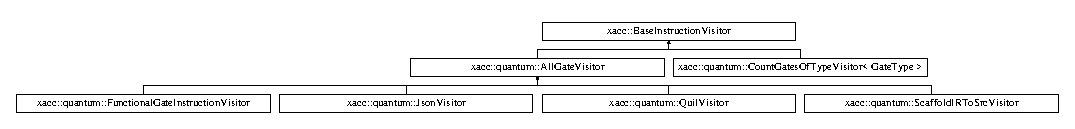
\includegraphics[height=1.288344cm]{a00018}
\end{center}
\end{figure}
\subsection*{Public Member Functions}
\begin{DoxyCompactItemize}
\item 
virtual \hyperlink{a00018_aa6f5104f5868fe1eca9be4dc4036eba4}{$\sim$\+Base\+Instruction\+Visitor} ()
\end{DoxyCompactItemize}


\subsection{Detailed Description}
The \hyperlink{a00018}{Base\+Instruction\+Visitor} is a base class for all classes that are \hyperlink{a00046}{Instruction} visitors. It basically provides a means for passing instruction visitor handles in a polymorphic manner. 

\subsection{Constructor \& Destructor Documentation}
\index{xacc\+::\+Base\+Instruction\+Visitor@{xacc\+::\+Base\+Instruction\+Visitor}!````~Base\+Instruction\+Visitor@{$\sim$\+Base\+Instruction\+Visitor}}
\index{````~Base\+Instruction\+Visitor@{$\sim$\+Base\+Instruction\+Visitor}!xacc\+::\+Base\+Instruction\+Visitor@{xacc\+::\+Base\+Instruction\+Visitor}}
\subsubsection[{\texorpdfstring{$\sim$\+Base\+Instruction\+Visitor()}{~BaseInstructionVisitor()}}]{\setlength{\rightskip}{0pt plus 5cm}virtual xacc\+::\+Base\+Instruction\+Visitor\+::$\sim$\+Base\+Instruction\+Visitor (
\begin{DoxyParamCaption}
{}
\end{DoxyParamCaption}
)\hspace{0.3cm}{\ttfamily [inline]}, {\ttfamily [virtual]}}\hypertarget{a00018_aa6f5104f5868fe1eca9be4dc4036eba4}{}\label{a00018_aa6f5104f5868fe1eca9be4dc4036eba4}
The destructor 

The documentation for this class was generated from the following file\+:\begin{DoxyCompactItemize}
\item 
Instruction\+Visitor.\+hpp\end{DoxyCompactItemize}

\chapter{2016-\/11-\/21-\/solving-\/problems}
\label{a00019}
\hypertarget{a00019}{}
\hypertarget{a00019}{}\section{xacc\+:\+:Accelerator\+Buffer Class Reference}
\label{a00019}\index{xacc\+::\+Accelerator\+Buffer@{xacc\+::\+Accelerator\+Buffer}}


{\ttfamily \#include $<$Accelerator\+Buffer.\+hpp$>$}

Inheritance diagram for xacc\+:\+:Accelerator\+Buffer\+:\begin{figure}[H]
\begin{center}
\leavevmode
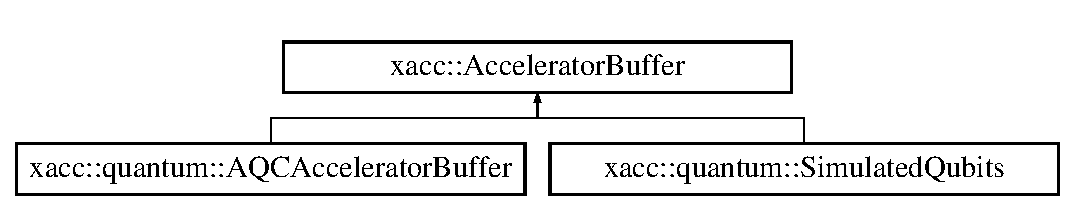
\includegraphics[height=2.000000cm]{a00019}
\end{center}
\end{figure}
\subsection*{Public Member Functions}
\begin{DoxyCompactItemize}
\item 
\hyperlink{a00019_ab606d8af942120d60b51a4fffcd75c98}{Accelerator\+Buffer} (const std\+::string \&str, const int N)
\item 
{\footnotesize template$<$typename... Indices$>$ }\\{\bfseries Accelerator\+Buffer} (const std\+::string \&str, int first\+Index, Indices...\+indices)\hypertarget{a00019_ac550d89390562095c56aa1b14ae85001}{}\label{a00019_ac550d89390562095c56aa1b14ae85001}

\item 
int {\bfseries size} ()\hypertarget{a00019_aa2a3101c2e3ae3550172bf49f9587f3b}{}\label{a00019_aa2a3101c2e3ae3550172bf49f9587f3b}

\item 
std\+::string {\bfseries name} ()\hypertarget{a00019_ad5b646e9efc21b6d0bcc22cd6f649c22}{}\label{a00019_ad5b646e9efc21b6d0bcc22cd6f649c22}

\item 
void {\bfseries reset\+Buffer} ()\hypertarget{a00019_aa6d6e9cfee6170333c1f03507345743f}{}\label{a00019_aa6d6e9cfee6170333c1f03507345743f}

\item 
void {\bfseries update\+Bit} (const int idx, int zero\+Or\+One)\hypertarget{a00019_a4bc0edbe9aa0d463f67ddcc38265066f}{}\label{a00019_a4bc0edbe9aa0d463f67ddcc38265066f}

\item 
void {\bfseries append\+Measurement} (const boost\+::dynamic\+\_\+bitset$<$$>$ \&measurement)\hypertarget{a00019_ac161c4f984f774d08197871094aabc67}{}\label{a00019_ac161c4f984f774d08197871094aabc67}

\item 
double {\bfseries get\+Average} () const \hypertarget{a00019_a97cf3cc4e1aaa8ac3cee7817860f77c1}{}\label{a00019_a97cf3cc4e1aaa8ac3cee7817860f77c1}

\item 
Accelerator\+Bit\+State {\bfseries get\+Accelerator\+Bit\+State} (const int idx)\hypertarget{a00019_aba6ef359f3117faa98f0eb8da90d909e}{}\label{a00019_aba6ef359f3117faa98f0eb8da90d909e}

\item 
virtual void {\bfseries print} ()\hypertarget{a00019_add0835e188f0eda4f1b68a28ddc79786}{}\label{a00019_add0835e188f0eda4f1b68a28ddc79786}

\item 
virtual void {\bfseries print} (std\+::ostream \&stream)\hypertarget{a00019_a7c59462451223772b41ef232b06a7dfa}{}\label{a00019_a7c59462451223772b41ef232b06a7dfa}

\end{DoxyCompactItemize}
\subsection*{Protected Attributes}
\begin{DoxyCompactItemize}
\item 
std\+::vector$<$ boost\+::dynamic\+\_\+bitset$<$$>$ $>$ {\bfseries measurements}\hypertarget{a00019_a5464b23a964985df2547f657877c9ea5}{}\label{a00019_a5464b23a964985df2547f657877c9ea5}

\item 
std\+::string {\bfseries buffer\+Id}\hypertarget{a00019_a3198e034d07d9b77b62da03e6592a221}{}\label{a00019_a3198e034d07d9b77b62da03e6592a221}

\item 
std\+::vector$<$ \hyperlink{a00018}{Accelerator\+Bit} $>$ {\bfseries bits}\hypertarget{a00019_ab6dbb8c22f8adc6aba34b00a84066854}{}\label{a00019_ab6dbb8c22f8adc6aba34b00a84066854}

\end{DoxyCompactItemize}


\subsection{Detailed Description}
The \hyperlink{a00019}{Accelerator\+Buffer} models an allocated buffer of bits that are operated on by a kernel. As such, the \hyperlink{a00019}{Accelerator\+Buffer}\textquotesingle{}s primary role is to store \hyperlink{a00017}{Accelerator} execution results.

\begin{DoxyAuthor}{Author}
Alex Mc\+Caskey 
\end{DoxyAuthor}


\subsection{Constructor \& Destructor Documentation}
\index{xacc\+::\+Accelerator\+Buffer@{xacc\+::\+Accelerator\+Buffer}!Accelerator\+Buffer@{Accelerator\+Buffer}}
\index{Accelerator\+Buffer@{Accelerator\+Buffer}!xacc\+::\+Accelerator\+Buffer@{xacc\+::\+Accelerator\+Buffer}}
\subsubsection[{\texorpdfstring{Accelerator\+Buffer(const std\+::string \&str, const int N)}{AcceleratorBuffer(const std::string \&str, const int N)}}]{\setlength{\rightskip}{0pt plus 5cm}xacc\+::\+Accelerator\+Buffer\+::\+Accelerator\+Buffer (
\begin{DoxyParamCaption}
\item[{const std\+::string \&}]{str, }
\item[{const int}]{N}
\end{DoxyParamCaption}
)\hspace{0.3cm}{\ttfamily [inline]}}\hypertarget{a00019_ab606d8af942120d60b51a4fffcd75c98}{}\label{a00019_ab606d8af942120d60b51a4fffcd75c98}
The Constructor 

The documentation for this class was generated from the following file\+:\begin{DoxyCompactItemize}
\item 
Accelerator\+Buffer.\+hpp\end{DoxyCompactItemize}

\chapter{about}
\label{a00020}
\hypertarget{a00020}{}
\hypertarget{a00020}{}\section{xacc\+:\+:Compiler Class Reference}
\label{a00020}\index{xacc\+::\+Compiler@{xacc\+::\+Compiler}}


{\ttfamily \#include $<$Compiler.\+hpp$>$}

Inheritance diagram for xacc\+:\+:Compiler\+:\begin{figure}[H]
\begin{center}
\leavevmode
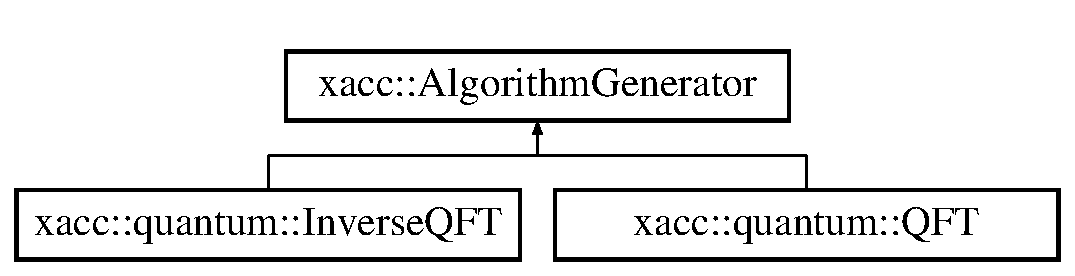
\includegraphics[height=2.772277cm]{a00020}
\end{center}
\end{figure}
\subsection*{Public Member Functions}
\begin{DoxyCompactItemize}
\item 
virtual std\+::shared\+\_\+ptr$<$ \hyperlink{a00041}{IR} $>$ \hyperlink{a00020_a546a40c95bb93af6a0c0ac48dbeaffc8}{compile} (const std\+::string \&src, std\+::shared\+\_\+ptr$<$ \hyperlink{a00011}{Accelerator} $>$ acc)=0
\item 
virtual std\+::shared\+\_\+ptr$<$ \hyperlink{a00041}{IR} $>$ \hyperlink{a00020_a9092f5f779b570c91569b59621280c04}{compile} (const std\+::string \&src)=0
\item 
virtual const std\+::string \hyperlink{a00020_a87fca9100e6462122f5b687c3a0fb3fb}{get\+Name} ()=0
\item 
virtual std\+::shared\+\_\+ptr$<$ options\+\_\+description $>$ \hyperlink{a00020_a9f5a8965c9c2dd895016d18264ebbe92}{get\+Options} ()
\item 
virtual \hyperlink{a00020_a5d0b012687d9b44893872eaa81e47b38}{$\sim$\+Compiler} ()
\end{DoxyCompactItemize}
\subsection*{Protected Attributes}
\begin{DoxyCompactItemize}
\item 
std\+::string \hyperlink{a00020_a0ad81c816c09e5113d03cdc02165c453}{kernel\+Source}
\item 
std\+::shared\+\_\+ptr$<$ \hyperlink{a00011}{Accelerator} $>$ \hyperlink{a00020_ad4cbb467fa7e377bac6c054ffcb22b7c}{accelerator}
\end{DoxyCompactItemize}


\subsection{Detailed Description}
The \hyperlink{a00020}{Compiler} class provides an extensible interface for injecting custom compilation mechanisms into the X\+A\+CC framework. Implementations provide a compile method that takes the kernel source code string, performs compiler-\/specific compilation mechanism, and returns a valid X\+A\+CC \hyperlink{a00041}{IR} instance modeling the result of the compilation. 

\subsection{Constructor \& Destructor Documentation}
\index{xacc\+::\+Compiler@{xacc\+::\+Compiler}!````~Compiler@{$\sim$\+Compiler}}
\index{````~Compiler@{$\sim$\+Compiler}!xacc\+::\+Compiler@{xacc\+::\+Compiler}}
\subsubsection[{\texorpdfstring{$\sim$\+Compiler()}{~Compiler()}}]{\setlength{\rightskip}{0pt plus 5cm}virtual xacc\+::\+Compiler\+::$\sim$\+Compiler (
\begin{DoxyParamCaption}
{}
\end{DoxyParamCaption}
)\hspace{0.3cm}{\ttfamily [inline]}, {\ttfamily [virtual]}}\hypertarget{a00020_a5d0b012687d9b44893872eaa81e47b38}{}\label{a00020_a5d0b012687d9b44893872eaa81e47b38}
The destructor 

\subsection{Member Function Documentation}
\index{xacc\+::\+Compiler@{xacc\+::\+Compiler}!compile@{compile}}
\index{compile@{compile}!xacc\+::\+Compiler@{xacc\+::\+Compiler}}
\subsubsection[{\texorpdfstring{compile(const std\+::string \&src, std\+::shared\+\_\+ptr$<$ Accelerator $>$ acc)=0}{compile(const std::string \&src, std::shared\_ptr< Accelerator > acc)=0}}]{\setlength{\rightskip}{0pt plus 5cm}virtual std\+::shared\+\_\+ptr$<${\bf IR}$>$ xacc\+::\+Compiler\+::compile (
\begin{DoxyParamCaption}
\item[{const std\+::string \&}]{src, }
\item[{std\+::shared\+\_\+ptr$<$ {\bf Accelerator} $>$}]{acc}
\end{DoxyParamCaption}
)\hspace{0.3cm}{\ttfamily [pure virtual]}}\hypertarget{a00020_a546a40c95bb93af6a0c0ac48dbeaffc8}{}\label{a00020_a546a40c95bb93af6a0c0ac48dbeaffc8}
This method is to be implemented by derived Compilers and is in charge of executing the compilation mechanism on the provided source string. Implementations also are given access to the \hyperlink{a00011}{Accelerator} that this source code is intended for.


\begin{DoxyParams}{Parameters}
{\em src} & The kernel source string. \\
\hline
{\em acc} & The \hyperlink{a00011}{Accelerator} this code will be executed on \\
\hline
\end{DoxyParams}
\begin{DoxyReturn}{Returns}
ir Intermediate representation for provided source kernel code. 
\end{DoxyReturn}


Implemented in \hyperlink{a00065_a7caede75bb2304ba405966651b115543}{xacc\+::quantum\+::\+Scaffold\+Compiler}, \hyperlink{a00050_a2421482415ca4e09963ea4ecddff8100}{xacc\+::quantum\+::\+Quil\+Compiler}, and \hyperlink{a00024_a0f7f6b10b4a881cb27b36eaa6d39e7b1}{xacc\+::quantum\+::\+D\+Wave\+Compiler}.

\index{xacc\+::\+Compiler@{xacc\+::\+Compiler}!compile@{compile}}
\index{compile@{compile}!xacc\+::\+Compiler@{xacc\+::\+Compiler}}
\subsubsection[{\texorpdfstring{compile(const std\+::string \&src)=0}{compile(const std::string \&src)=0}}]{\setlength{\rightskip}{0pt plus 5cm}virtual std\+::shared\+\_\+ptr$<${\bf IR}$>$ xacc\+::\+Compiler\+::compile (
\begin{DoxyParamCaption}
\item[{const std\+::string \&}]{src}
\end{DoxyParamCaption}
)\hspace{0.3cm}{\ttfamily [pure virtual]}}\hypertarget{a00020_a9092f5f779b570c91569b59621280c04}{}\label{a00020_a9092f5f779b570c91569b59621280c04}
This method is to be implemented by derived Compilers and is in charge of executing the compilation mechanism on the provided source string. 
\begin{DoxyParams}{Parameters}
{\em src} & \\
\hline
\end{DoxyParams}
\begin{DoxyReturn}{Returns}

\end{DoxyReturn}


Implemented in \hyperlink{a00065_a3736ecc229fe6acdd4c991e85d7a1f08}{xacc\+::quantum\+::\+Scaffold\+Compiler}, \hyperlink{a00050_adf4d321ecb0df3fa7728999f941c83b2}{xacc\+::quantum\+::\+Quil\+Compiler}, and \hyperlink{a00024_a893e1d1c81a8aaf6e2435c9bceab575e}{xacc\+::quantum\+::\+D\+Wave\+Compiler}.

\index{xacc\+::\+Compiler@{xacc\+::\+Compiler}!get\+Name@{get\+Name}}
\index{get\+Name@{get\+Name}!xacc\+::\+Compiler@{xacc\+::\+Compiler}}
\subsubsection[{\texorpdfstring{get\+Name()=0}{getName()=0}}]{\setlength{\rightskip}{0pt plus 5cm}virtual const std\+::string xacc\+::\+Compiler\+::get\+Name (
\begin{DoxyParamCaption}
{}
\end{DoxyParamCaption}
)\hspace{0.3cm}{\ttfamily [pure virtual]}}\hypertarget{a00020_a87fca9100e6462122f5b687c3a0fb3fb}{}\label{a00020_a87fca9100e6462122f5b687c3a0fb3fb}
Return the name of this \hyperlink{a00020}{Compiler} \begin{DoxyReturn}{Returns}
name \hyperlink{a00020}{Compiler} name 
\end{DoxyReturn}


Implemented in \hyperlink{a00065_a3f537054a3924a1d14f4ceb0f0181161}{xacc\+::quantum\+::\+Scaffold\+Compiler}, \hyperlink{a00050_ae7d52140b6dd52730edc6e38ae48f437}{xacc\+::quantum\+::\+Quil\+Compiler}, and \hyperlink{a00024_a8a180031ae563e1a9aac611e8066c181}{xacc\+::quantum\+::\+D\+Wave\+Compiler}.

\index{xacc\+::\+Compiler@{xacc\+::\+Compiler}!get\+Options@{get\+Options}}
\index{get\+Options@{get\+Options}!xacc\+::\+Compiler@{xacc\+::\+Compiler}}
\subsubsection[{\texorpdfstring{get\+Options()}{getOptions()}}]{\setlength{\rightskip}{0pt plus 5cm}virtual std\+::shared\+\_\+ptr$<$options\+\_\+description$>$ xacc\+::\+Compiler\+::get\+Options (
\begin{DoxyParamCaption}
{}
\end{DoxyParamCaption}
)\hspace{0.3cm}{\ttfamily [inline]}, {\ttfamily [virtual]}}\hypertarget{a00020_a9f5a8965c9c2dd895016d18264ebbe92}{}\label{a00020_a9f5a8965c9c2dd895016d18264ebbe92}
Return an empty options\+\_\+description, this is for subclasses to implement. 

Implements \hyperlink{a00046_a6d150954f852109bfe2c1ae90222926f}{xacc\+::\+Options\+Provider}.



\subsection{Member Data Documentation}
\index{xacc\+::\+Compiler@{xacc\+::\+Compiler}!accelerator@{accelerator}}
\index{accelerator@{accelerator}!xacc\+::\+Compiler@{xacc\+::\+Compiler}}
\subsubsection[{\texorpdfstring{accelerator}{accelerator}}]{\setlength{\rightskip}{0pt plus 5cm}std\+::shared\+\_\+ptr$<${\bf Accelerator}$>$ xacc\+::\+Compiler\+::accelerator\hspace{0.3cm}{\ttfamily [protected]}}\hypertarget{a00020_ad4cbb467fa7e377bac6c054ffcb22b7c}{}\label{a00020_ad4cbb467fa7e377bac6c054ffcb22b7c}
Reference to the \hyperlink{a00011}{Accelerator} that this compiler is targeting. \index{xacc\+::\+Compiler@{xacc\+::\+Compiler}!kernel\+Source@{kernel\+Source}}
\index{kernel\+Source@{kernel\+Source}!xacc\+::\+Compiler@{xacc\+::\+Compiler}}
\subsubsection[{\texorpdfstring{kernel\+Source}{kernelSource}}]{\setlength{\rightskip}{0pt plus 5cm}std\+::string xacc\+::\+Compiler\+::kernel\+Source\hspace{0.3cm}{\ttfamily [protected]}}\hypertarget{a00020_a0ad81c816c09e5113d03cdc02165c453}{}\label{a00020_a0ad81c816c09e5113d03cdc02165c453}
Reference to the provided kernel source code string 

The documentation for this class was generated from the following file\+:\begin{DoxyCompactItemize}
\item 
Compiler.\+hpp\end{DoxyCompactItemize}

\chapter{design}
\label{a00021}
\hypertarget{a00021}{}
\hypertarget{a00021}{}\section{xacc\+:\+:quantum\+:\+:All\+Gate\+Visitor Class Reference}
\label{a00021}\index{xacc\+::quantum\+::\+All\+Gate\+Visitor@{xacc\+::quantum\+::\+All\+Gate\+Visitor}}


{\ttfamily \#include $<$All\+Gate\+Visitor.\+hpp$>$}

Inheritance diagram for xacc\+:\+:quantum\+:\+:All\+Gate\+Visitor\+:\begin{figure}[H]
\begin{center}
\leavevmode
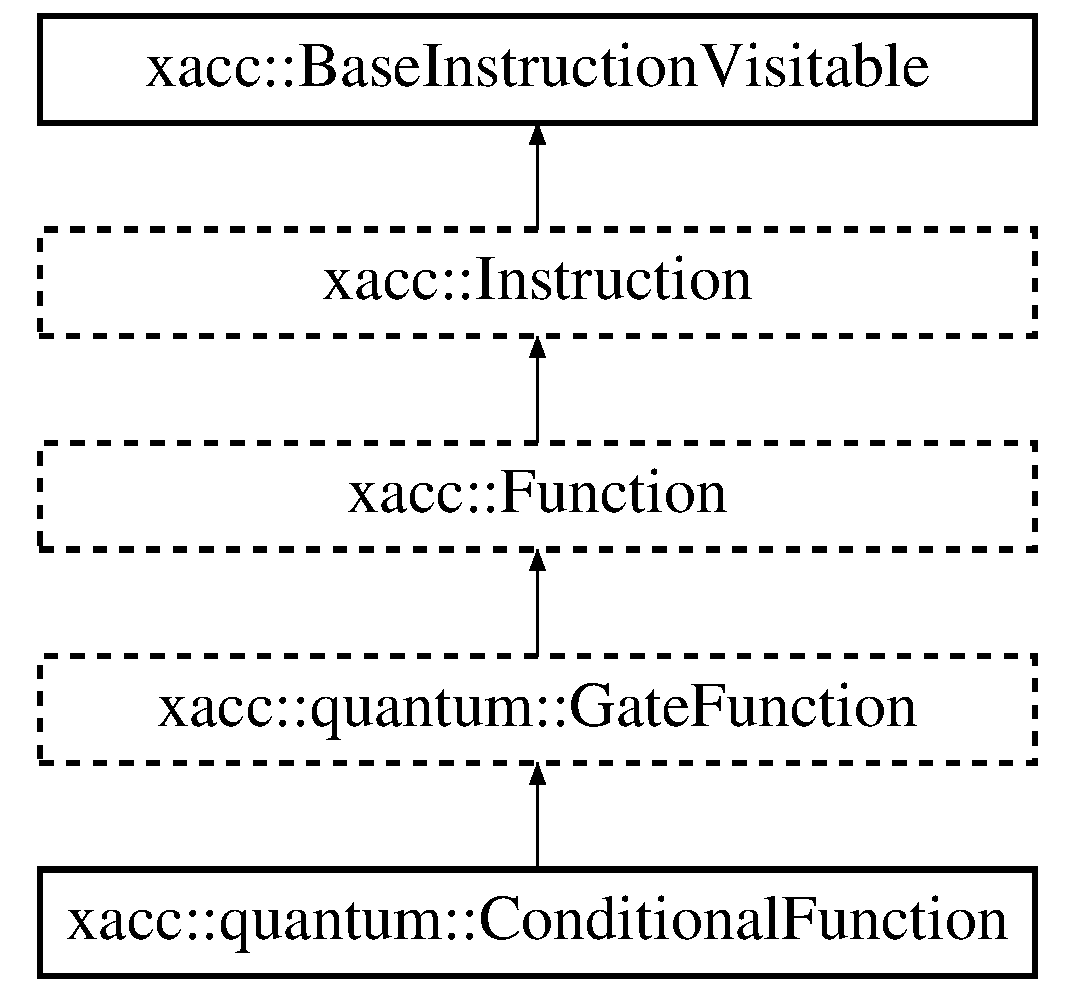
\includegraphics[height=7.887324cm]{a00021}
\end{center}
\end{figure}
\subsection*{Additional Inherited Members}


\subsection{Detailed Description}
F\+I\+X\+ME write this 

The documentation for this class was generated from the following file\+:\begin{DoxyCompactItemize}
\item 
All\+Gate\+Visitor.\+hpp\end{DoxyCompactItemize}

\chapter{Gravity}
\label{a00022}
\hypertarget{a00022}{}
\hypertarget{a00022}{}\section{xacc\+:\+:quantum\+:\+:A\+Q\+C\+Accelerator\+Buffer Class Reference}
\label{a00022}\index{xacc\+::quantum\+::\+A\+Q\+C\+Accelerator\+Buffer@{xacc\+::quantum\+::\+A\+Q\+C\+Accelerator\+Buffer}}


{\ttfamily \#include $<$A\+Q\+C\+Accelerator\+Buffer.\+hpp$>$}

Inheritance diagram for xacc\+:\+:quantum\+:\+:A\+Q\+C\+Accelerator\+Buffer\+:\begin{figure}[H]
\begin{center}
\leavevmode
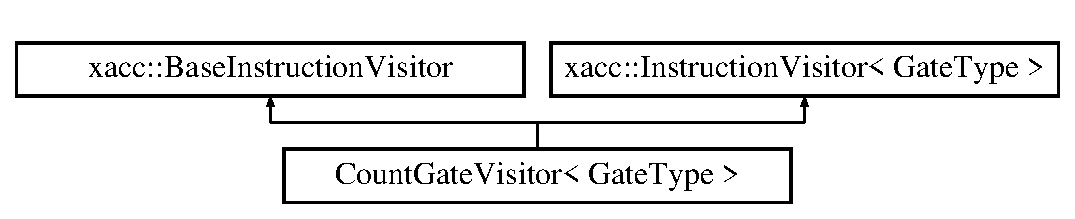
\includegraphics[height=2.000000cm]{a00022}
\end{center}
\end{figure}
\subsection*{Public Member Functions}
\begin{DoxyCompactItemize}
\item 
\hyperlink{a00022_ac2f9ea58140a27741b4dc8fceaa1ca5c}{A\+Q\+C\+Accelerator\+Buffer} (const std\+::string \&str, const int N)
\item 
{\footnotesize template$<$typename... Indices$>$ }\\\hyperlink{a00022_a628c742acf1d20fc8fe9b69f9be7b2c6}{A\+Q\+C\+Accelerator\+Buffer} (const std\+::string \&str, int first\+Index, Indices...\+indices)
\item 
void \hyperlink{a00022_a23992d11bdb6f093c0ce3f743677d4d9}{set\+Embedding} (std\+::map$<$ int, std\+::list$<$ int $>$$>$ emb)
\item 
std\+::map$<$ int, std\+::list$<$ int $>$ $>$ \hyperlink{a00022_ae98155c023d1b31b3b55a8c8e4ec6bc6}{get\+Embedding} ()
\end{DoxyCompactItemize}
\subsection*{Protected Attributes}
\begin{DoxyCompactItemize}
\item 
std\+::map$<$ int, std\+::list$<$ int $>$ $>$ \hyperlink{a00022_a26fd739244b0346cc3398eef31b11264}{embedding}
\item 
std\+::vector$<$ double $>$ \hyperlink{a00022_abe6d781724e197df449d8dfcde60e1a4}{energies}
\end{DoxyCompactItemize}


\subsection{Detailed Description}
The \hyperlink{a00022}{A\+Q\+C\+Accelerator\+Buffer} is an \hyperlink{a00019}{Accelerator\+Buffer} that keeps track of the problem-\/specific embedding into the hardware graph. It also tracks A\+QC Q\+PU computed energies. 

\subsection{Constructor \& Destructor Documentation}
\index{xacc\+::quantum\+::\+A\+Q\+C\+Accelerator\+Buffer@{xacc\+::quantum\+::\+A\+Q\+C\+Accelerator\+Buffer}!A\+Q\+C\+Accelerator\+Buffer@{A\+Q\+C\+Accelerator\+Buffer}}
\index{A\+Q\+C\+Accelerator\+Buffer@{A\+Q\+C\+Accelerator\+Buffer}!xacc\+::quantum\+::\+A\+Q\+C\+Accelerator\+Buffer@{xacc\+::quantum\+::\+A\+Q\+C\+Accelerator\+Buffer}}
\subsubsection[{\texorpdfstring{A\+Q\+C\+Accelerator\+Buffer(const std\+::string \&str, const int N)}{AQCAcceleratorBuffer(const std::string \&str, const int N)}}]{\setlength{\rightskip}{0pt plus 5cm}xacc\+::quantum\+::\+A\+Q\+C\+Accelerator\+Buffer\+::\+A\+Q\+C\+Accelerator\+Buffer (
\begin{DoxyParamCaption}
\item[{const std\+::string \&}]{str, }
\item[{const int}]{N}
\end{DoxyParamCaption}
)\hspace{0.3cm}{\ttfamily [inline]}}\hypertarget{a00022_ac2f9ea58140a27741b4dc8fceaa1ca5c}{}\label{a00022_ac2f9ea58140a27741b4dc8fceaa1ca5c}
The constructor 
\begin{DoxyParams}{Parameters}
{\em str} & The name of this buffer \\
\hline
{\em N} & The number of bits represented by this buffer \\
\hline
\end{DoxyParams}
\index{xacc\+::quantum\+::\+A\+Q\+C\+Accelerator\+Buffer@{xacc\+::quantum\+::\+A\+Q\+C\+Accelerator\+Buffer}!A\+Q\+C\+Accelerator\+Buffer@{A\+Q\+C\+Accelerator\+Buffer}}
\index{A\+Q\+C\+Accelerator\+Buffer@{A\+Q\+C\+Accelerator\+Buffer}!xacc\+::quantum\+::\+A\+Q\+C\+Accelerator\+Buffer@{xacc\+::quantum\+::\+A\+Q\+C\+Accelerator\+Buffer}}
\subsubsection[{\texorpdfstring{A\+Q\+C\+Accelerator\+Buffer(const std\+::string \&str, int first\+Index, Indices...\+indices)}{AQCAcceleratorBuffer(const std::string \&str, int firstIndex, Indices...indices)}}]{\setlength{\rightskip}{0pt plus 5cm}template$<$typename... Indices$>$ xacc\+::quantum\+::\+A\+Q\+C\+Accelerator\+Buffer\+::\+A\+Q\+C\+Accelerator\+Buffer (
\begin{DoxyParamCaption}
\item[{const std\+::string \&}]{str, }
\item[{int}]{first\+Index, }
\item[{Indices...}]{indices}
\end{DoxyParamCaption}
)\hspace{0.3cm}{\ttfamily [inline]}}\hypertarget{a00022_a628c742acf1d20fc8fe9b69f9be7b2c6}{}\label{a00022_a628c742acf1d20fc8fe9b69f9be7b2c6}
The constructor 
\begin{DoxyParams}{Parameters}
{\em str} & \\
\hline
{\em first\+Index} & \\
\hline
{\em indices} & \\
\hline
\end{DoxyParams}


\subsection{Member Function Documentation}
\index{xacc\+::quantum\+::\+A\+Q\+C\+Accelerator\+Buffer@{xacc\+::quantum\+::\+A\+Q\+C\+Accelerator\+Buffer}!get\+Embedding@{get\+Embedding}}
\index{get\+Embedding@{get\+Embedding}!xacc\+::quantum\+::\+A\+Q\+C\+Accelerator\+Buffer@{xacc\+::quantum\+::\+A\+Q\+C\+Accelerator\+Buffer}}
\subsubsection[{\texorpdfstring{get\+Embedding()}{getEmbedding()}}]{\setlength{\rightskip}{0pt plus 5cm}std\+::map$<$int, std\+::list$<$int$>$ $>$ xacc\+::quantum\+::\+A\+Q\+C\+Accelerator\+Buffer\+::get\+Embedding (
\begin{DoxyParamCaption}
{}
\end{DoxyParamCaption}
)\hspace{0.3cm}{\ttfamily [inline]}}\hypertarget{a00022_ae98155c023d1b31b3b55a8c8e4ec6bc6}{}\label{a00022_ae98155c023d1b31b3b55a8c8e4ec6bc6}
Return the minor graph embedding.

\begin{DoxyReturn}{Returns}
emb The minor graph embedding 
\end{DoxyReturn}
\index{xacc\+::quantum\+::\+A\+Q\+C\+Accelerator\+Buffer@{xacc\+::quantum\+::\+A\+Q\+C\+Accelerator\+Buffer}!set\+Embedding@{set\+Embedding}}
\index{set\+Embedding@{set\+Embedding}!xacc\+::quantum\+::\+A\+Q\+C\+Accelerator\+Buffer@{xacc\+::quantum\+::\+A\+Q\+C\+Accelerator\+Buffer}}
\subsubsection[{\texorpdfstring{set\+Embedding(std\+::map$<$ int, std\+::list$<$ int $>$$>$ emb)}{setEmbedding(std::map< int, std::list< int >> emb)}}]{\setlength{\rightskip}{0pt plus 5cm}void xacc\+::quantum\+::\+A\+Q\+C\+Accelerator\+Buffer\+::set\+Embedding (
\begin{DoxyParamCaption}
\item[{std\+::map$<$ int, std\+::list$<$ int $>$$>$}]{emb}
\end{DoxyParamCaption}
)\hspace{0.3cm}{\ttfamily [inline]}}\hypertarget{a00022_a23992d11bdb6f093c0ce3f743677d4d9}{}\label{a00022_a23992d11bdb6f093c0ce3f743677d4d9}
Set the minor graph embedding for the problem solved during this execution .


\begin{DoxyParams}{Parameters}
{\em emb} & The minor graph embedding \\
\hline
\end{DoxyParams}


\subsection{Member Data Documentation}
\index{xacc\+::quantum\+::\+A\+Q\+C\+Accelerator\+Buffer@{xacc\+::quantum\+::\+A\+Q\+C\+Accelerator\+Buffer}!embedding@{embedding}}
\index{embedding@{embedding}!xacc\+::quantum\+::\+A\+Q\+C\+Accelerator\+Buffer@{xacc\+::quantum\+::\+A\+Q\+C\+Accelerator\+Buffer}}
\subsubsection[{\texorpdfstring{embedding}{embedding}}]{\setlength{\rightskip}{0pt plus 5cm}std\+::map$<$int, std\+::list$<$int$>$ $>$ xacc\+::quantum\+::\+A\+Q\+C\+Accelerator\+Buffer\+::embedding\hspace{0.3cm}{\ttfamily [protected]}}\hypertarget{a00022_a26fd739244b0346cc3398eef31b11264}{}\label{a00022_a26fd739244b0346cc3398eef31b11264}
The minor graph embedding for the problem these results represent. \index{xacc\+::quantum\+::\+A\+Q\+C\+Accelerator\+Buffer@{xacc\+::quantum\+::\+A\+Q\+C\+Accelerator\+Buffer}!energies@{energies}}
\index{energies@{energies}!xacc\+::quantum\+::\+A\+Q\+C\+Accelerator\+Buffer@{xacc\+::quantum\+::\+A\+Q\+C\+Accelerator\+Buffer}}
\subsubsection[{\texorpdfstring{energies}{energies}}]{\setlength{\rightskip}{0pt plus 5cm}std\+::vector$<$double$>$ xacc\+::quantum\+::\+A\+Q\+C\+Accelerator\+Buffer\+::energies\hspace{0.3cm}{\ttfamily [protected]}}\hypertarget{a00022_abe6d781724e197df449d8dfcde60e1a4}{}\label{a00022_abe6d781724e197df449d8dfcde60e1a4}
The energies computed as part of this execution. 

The documentation for this class was generated from the following file\+:\begin{DoxyCompactItemize}
\item 
A\+Q\+C\+Accelerator\+Buffer.\+hpp\end{DoxyCompactItemize}

\chapter{science}
\label{a00023}
\hypertarget{a00023}{}
\hypertarget{a00023}{}\section{xacc\+:\+:Compiler Class Reference}
\label{a00023}\index{xacc\+::\+Compiler@{xacc\+::\+Compiler}}


{\ttfamily \#include $<$Compiler.\+hpp$>$}

Inheritance diagram for xacc\+:\+:Compiler\+:\begin{figure}[H]
\begin{center}
\leavevmode
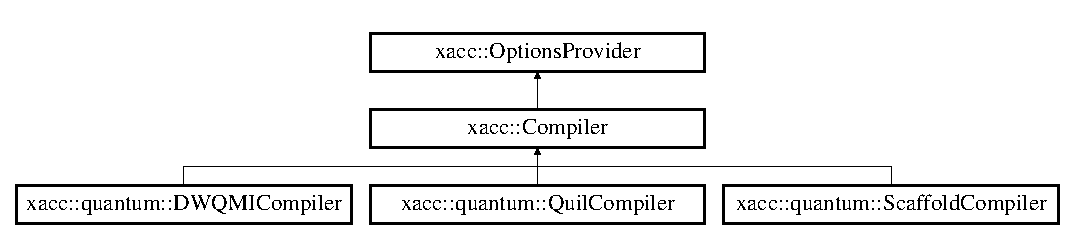
\includegraphics[height=2.772277cm]{a00023}
\end{center}
\end{figure}
\subsection*{Public Member Functions}
\begin{DoxyCompactItemize}
\item 
virtual std\+::shared\+\_\+ptr$<$ \hyperlink{a00051}{IR} $>$ \hyperlink{a00023_a546a40c95bb93af6a0c0ac48dbeaffc8}{compile} (const std\+::string \&src, std\+::shared\+\_\+ptr$<$ \hyperlink{a00011}{Accelerator} $>$ acc)=0
\item 
virtual std\+::shared\+\_\+ptr$<$ \hyperlink{a00051}{IR} $>$ \hyperlink{a00023_a9092f5f779b570c91569b59621280c04}{compile} (const std\+::string \&src)=0
\item 
virtual const std\+::string \hyperlink{a00023_aeedbe58a33fed29e4d7694ae743e25e7}{translate} (const std\+::string \&buffer\+Variable, std\+::shared\+\_\+ptr$<$ \hyperlink{a00039}{Function} $>$ function)=0
\item 
virtual const std\+::string \hyperlink{a00023_a87fca9100e6462122f5b687c3a0fb3fb}{get\+Name} ()=0
\item 
virtual std\+::shared\+\_\+ptr$<$ options\+\_\+description $>$ \hyperlink{a00023_a9f5a8965c9c2dd895016d18264ebbe92}{get\+Options} ()
\item 
virtual \hyperlink{a00023_a5d0b012687d9b44893872eaa81e47b38}{$\sim$\+Compiler} ()
\end{DoxyCompactItemize}
\subsection*{Protected Attributes}
\begin{DoxyCompactItemize}
\item 
std\+::string \hyperlink{a00023_a0ad81c816c09e5113d03cdc02165c453}{kernel\+Source}
\item 
std\+::shared\+\_\+ptr$<$ \hyperlink{a00011}{Accelerator} $>$ \hyperlink{a00023_ad4cbb467fa7e377bac6c054ffcb22b7c}{accelerator}
\end{DoxyCompactItemize}


\subsection{Detailed Description}
The \hyperlink{a00023}{Compiler} class provides an extensible interface for injecting custom compilation mechanisms into the X\+A\+CC framework. Implementations provide a compile method that takes the kernel source code string, performs compiler-\/specific compilation mechanism, and returns a valid X\+A\+CC \hyperlink{a00051}{IR} instance modeling the result of the compilation. 

\subsection{Constructor \& Destructor Documentation}
\index{xacc\+::\+Compiler@{xacc\+::\+Compiler}!````~Compiler@{$\sim$\+Compiler}}
\index{````~Compiler@{$\sim$\+Compiler}!xacc\+::\+Compiler@{xacc\+::\+Compiler}}
\subsubsection[{\texorpdfstring{$\sim$\+Compiler()}{~Compiler()}}]{\setlength{\rightskip}{0pt plus 5cm}virtual xacc\+::\+Compiler\+::$\sim$\+Compiler (
\begin{DoxyParamCaption}
{}
\end{DoxyParamCaption}
)\hspace{0.3cm}{\ttfamily [inline]}, {\ttfamily [virtual]}}\hypertarget{a00023_a5d0b012687d9b44893872eaa81e47b38}{}\label{a00023_a5d0b012687d9b44893872eaa81e47b38}
The destructor 

\subsection{Member Function Documentation}
\index{xacc\+::\+Compiler@{xacc\+::\+Compiler}!compile@{compile}}
\index{compile@{compile}!xacc\+::\+Compiler@{xacc\+::\+Compiler}}
\subsubsection[{\texorpdfstring{compile(const std\+::string \&src, std\+::shared\+\_\+ptr$<$ Accelerator $>$ acc)=0}{compile(const std::string \&src, std::shared\_ptr< Accelerator > acc)=0}}]{\setlength{\rightskip}{0pt plus 5cm}virtual std\+::shared\+\_\+ptr$<${\bf IR}$>$ xacc\+::\+Compiler\+::compile (
\begin{DoxyParamCaption}
\item[{const std\+::string \&}]{src, }
\item[{std\+::shared\+\_\+ptr$<$ {\bf Accelerator} $>$}]{acc}
\end{DoxyParamCaption}
)\hspace{0.3cm}{\ttfamily [pure virtual]}}\hypertarget{a00023_a546a40c95bb93af6a0c0ac48dbeaffc8}{}\label{a00023_a546a40c95bb93af6a0c0ac48dbeaffc8}
This method is to be implemented by derived Compilers and is in charge of executing the compilation mechanism on the provided source string. Implementations also are given access to the \hyperlink{a00011}{Accelerator} that this source code is intended for.


\begin{DoxyParams}{Parameters}
{\em src} & The kernel source string. \\
\hline
{\em acc} & The \hyperlink{a00011}{Accelerator} this code will be executed on \\
\hline
\end{DoxyParams}
\begin{DoxyReturn}{Returns}
ir Intermediate representation for provided source kernel code. 
\end{DoxyReturn}


Implemented in \hyperlink{a00034_a0df05642f1a6fd44ce7f1c0396d50c9c}{xacc\+::quantum\+::\+D\+W\+Q\+M\+I\+Compiler}, \hyperlink{a00078_a7caede75bb2304ba405966651b115543}{xacc\+::quantum\+::\+Scaffold\+Compiler}, and \hyperlink{a00063_a2421482415ca4e09963ea4ecddff8100}{xacc\+::quantum\+::\+Quil\+Compiler}.

\index{xacc\+::\+Compiler@{xacc\+::\+Compiler}!compile@{compile}}
\index{compile@{compile}!xacc\+::\+Compiler@{xacc\+::\+Compiler}}
\subsubsection[{\texorpdfstring{compile(const std\+::string \&src)=0}{compile(const std::string \&src)=0}}]{\setlength{\rightskip}{0pt plus 5cm}virtual std\+::shared\+\_\+ptr$<${\bf IR}$>$ xacc\+::\+Compiler\+::compile (
\begin{DoxyParamCaption}
\item[{const std\+::string \&}]{src}
\end{DoxyParamCaption}
)\hspace{0.3cm}{\ttfamily [pure virtual]}}\hypertarget{a00023_a9092f5f779b570c91569b59621280c04}{}\label{a00023_a9092f5f779b570c91569b59621280c04}
This method is to be implemented by derived Compilers and is in charge of executing the compilation mechanism on the provided source string. 
\begin{DoxyParams}{Parameters}
{\em src} & \\
\hline
\end{DoxyParams}
\begin{DoxyReturn}{Returns}

\end{DoxyReturn}


Implemented in \hyperlink{a00034_aa22591343b5509bf2c3a5820130ba906}{xacc\+::quantum\+::\+D\+W\+Q\+M\+I\+Compiler}, \hyperlink{a00078_a3736ecc229fe6acdd4c991e85d7a1f08}{xacc\+::quantum\+::\+Scaffold\+Compiler}, and \hyperlink{a00063_adf4d321ecb0df3fa7728999f941c83b2}{xacc\+::quantum\+::\+Quil\+Compiler}.

\index{xacc\+::\+Compiler@{xacc\+::\+Compiler}!get\+Name@{get\+Name}}
\index{get\+Name@{get\+Name}!xacc\+::\+Compiler@{xacc\+::\+Compiler}}
\subsubsection[{\texorpdfstring{get\+Name()=0}{getName()=0}}]{\setlength{\rightskip}{0pt plus 5cm}virtual const std\+::string xacc\+::\+Compiler\+::get\+Name (
\begin{DoxyParamCaption}
{}
\end{DoxyParamCaption}
)\hspace{0.3cm}{\ttfamily [pure virtual]}}\hypertarget{a00023_a87fca9100e6462122f5b687c3a0fb3fb}{}\label{a00023_a87fca9100e6462122f5b687c3a0fb3fb}
Return the name of this \hyperlink{a00023}{Compiler} \begin{DoxyReturn}{Returns}
name \hyperlink{a00023}{Compiler} name 
\end{DoxyReturn}


Implemented in \hyperlink{a00034_aed42de96f8e0dd94b6de183f28aee419}{xacc\+::quantum\+::\+D\+W\+Q\+M\+I\+Compiler}, \hyperlink{a00078_a3f537054a3924a1d14f4ceb0f0181161}{xacc\+::quantum\+::\+Scaffold\+Compiler}, and \hyperlink{a00063_ae7d52140b6dd52730edc6e38ae48f437}{xacc\+::quantum\+::\+Quil\+Compiler}.

\index{xacc\+::\+Compiler@{xacc\+::\+Compiler}!get\+Options@{get\+Options}}
\index{get\+Options@{get\+Options}!xacc\+::\+Compiler@{xacc\+::\+Compiler}}
\subsubsection[{\texorpdfstring{get\+Options()}{getOptions()}}]{\setlength{\rightskip}{0pt plus 5cm}virtual std\+::shared\+\_\+ptr$<$options\+\_\+description$>$ xacc\+::\+Compiler\+::get\+Options (
\begin{DoxyParamCaption}
{}
\end{DoxyParamCaption}
)\hspace{0.3cm}{\ttfamily [inline]}, {\ttfamily [virtual]}}\hypertarget{a00023_a9f5a8965c9c2dd895016d18264ebbe92}{}\label{a00023_a9f5a8965c9c2dd895016d18264ebbe92}
Return an empty options\+\_\+description, this is for subclasses to implement. 

Implements \hyperlink{a00057_a6d150954f852109bfe2c1ae90222926f}{xacc\+::\+Options\+Provider}.



Reimplemented in \hyperlink{a00034_a0851334cc33b5b1da2694150a0a1a43c}{xacc\+::quantum\+::\+D\+W\+Q\+M\+I\+Compiler}.

\index{xacc\+::\+Compiler@{xacc\+::\+Compiler}!translate@{translate}}
\index{translate@{translate}!xacc\+::\+Compiler@{xacc\+::\+Compiler}}
\subsubsection[{\texorpdfstring{translate(const std\+::string \&buffer\+Variable, std\+::shared\+\_\+ptr$<$ Function $>$ function)=0}{translate(const std::string \&bufferVariable, std::shared\_ptr< Function > function)=0}}]{\setlength{\rightskip}{0pt plus 5cm}virtual const std\+::string xacc\+::\+Compiler\+::translate (
\begin{DoxyParamCaption}
\item[{const std\+::string \&}]{buffer\+Variable, }
\item[{std\+::shared\+\_\+ptr$<$ {\bf Function} $>$}]{function}
\end{DoxyParamCaption}
)\hspace{0.3cm}{\ttfamily [pure virtual]}}\hypertarget{a00023_aeedbe58a33fed29e4d7694ae743e25e7}{}\label{a00023_aeedbe58a33fed29e4d7694ae743e25e7}
This method is to be implemented by derived Compilers and is in charge of taking the provided \hyperlink{a00039}{Function} \hyperlink{a00051}{IR} and converting it to source code in this \hyperlink{a00023}{Compiler}\textquotesingle{}s language.


\begin{DoxyParams}{Parameters}
{\em function} & The X\+A\+CC \hyperlink{a00051}{IR} \hyperlink{a00039}{Function} to translate \\
\hline
\end{DoxyParams}
\begin{DoxyReturn}{Returns}
src The source code as a string 
\end{DoxyReturn}


Implemented in \hyperlink{a00034_a56a345539665099329209b3b5f6810c9}{xacc\+::quantum\+::\+D\+W\+Q\+M\+I\+Compiler}, \hyperlink{a00063_a66ca00bbb1f30e7bc6dd86b1e267b93b}{xacc\+::quantum\+::\+Quil\+Compiler}, and \hyperlink{a00078_ac7ca2941e987ba579c6f50cfbd7fb0dc}{xacc\+::quantum\+::\+Scaffold\+Compiler}.



\subsection{Member Data Documentation}
\index{xacc\+::\+Compiler@{xacc\+::\+Compiler}!accelerator@{accelerator}}
\index{accelerator@{accelerator}!xacc\+::\+Compiler@{xacc\+::\+Compiler}}
\subsubsection[{\texorpdfstring{accelerator}{accelerator}}]{\setlength{\rightskip}{0pt plus 5cm}std\+::shared\+\_\+ptr$<${\bf Accelerator}$>$ xacc\+::\+Compiler\+::accelerator\hspace{0.3cm}{\ttfamily [protected]}}\hypertarget{a00023_ad4cbb467fa7e377bac6c054ffcb22b7c}{}\label{a00023_ad4cbb467fa7e377bac6c054ffcb22b7c}
Reference to the \hyperlink{a00011}{Accelerator} that this compiler is targeting. \index{xacc\+::\+Compiler@{xacc\+::\+Compiler}!kernel\+Source@{kernel\+Source}}
\index{kernel\+Source@{kernel\+Source}!xacc\+::\+Compiler@{xacc\+::\+Compiler}}
\subsubsection[{\texorpdfstring{kernel\+Source}{kernelSource}}]{\setlength{\rightskip}{0pt plus 5cm}std\+::string xacc\+::\+Compiler\+::kernel\+Source\hspace{0.3cm}{\ttfamily [protected]}}\hypertarget{a00023_a0ad81c816c09e5113d03cdc02165c453}{}\label{a00023_a0ad81c816c09e5113d03cdc02165c453}
Reference to the provided kernel source code string 

The documentation for this class was generated from the following file\+:\begin{DoxyCompactItemize}
\item 
Compiler.\+hpp\end{DoxyCompactItemize}

\chapter{Fire Framework}
\label{a00024}
\hypertarget{a00024}{}
\hypertarget{a00024}{}\section{xacc\+:\+:Base\+Instruction\+Visitor Class Reference}
\label{a00024}\index{xacc\+::\+Base\+Instruction\+Visitor@{xacc\+::\+Base\+Instruction\+Visitor}}


{\ttfamily \#include $<$Instruction\+Visitor.\+hpp$>$}

Inheritance diagram for xacc\+:\+:Base\+Instruction\+Visitor\+:\begin{figure}[H]
\begin{center}
\leavevmode
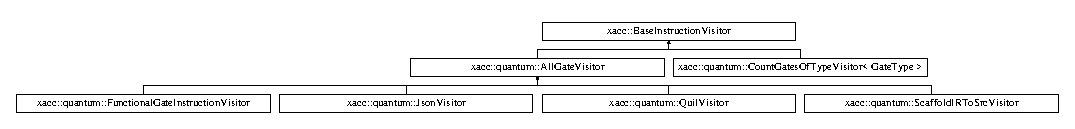
\includegraphics[height=1.288344cm]{a00024}
\end{center}
\end{figure}
\subsection*{Public Member Functions}
\begin{DoxyCompactItemize}
\item 
virtual \hyperlink{a00024_aa6f5104f5868fe1eca9be4dc4036eba4}{$\sim$\+Base\+Instruction\+Visitor} ()
\end{DoxyCompactItemize}


\subsection{Detailed Description}
The \hyperlink{a00024}{Base\+Instruction\+Visitor} is a base class for all classes that are \hyperlink{a00072}{Instruction} visitors. It basically provides a means for passing instruction visitor handles in a polymorphic manner. 

\subsection{Constructor \& Destructor Documentation}
\index{xacc\+::\+Base\+Instruction\+Visitor@{xacc\+::\+Base\+Instruction\+Visitor}!````~Base\+Instruction\+Visitor@{$\sim$\+Base\+Instruction\+Visitor}}
\index{````~Base\+Instruction\+Visitor@{$\sim$\+Base\+Instruction\+Visitor}!xacc\+::\+Base\+Instruction\+Visitor@{xacc\+::\+Base\+Instruction\+Visitor}}
\subsubsection[{\texorpdfstring{$\sim$\+Base\+Instruction\+Visitor()}{~BaseInstructionVisitor()}}]{\setlength{\rightskip}{0pt plus 5cm}virtual xacc\+::\+Base\+Instruction\+Visitor\+::$\sim$\+Base\+Instruction\+Visitor (
\begin{DoxyParamCaption}
{}
\end{DoxyParamCaption}
)\hspace{0.3cm}{\ttfamily [inline]}, {\ttfamily [virtual]}}\hypertarget{a00024_aa6f5104f5868fe1eca9be4dc4036eba4}{}\label{a00024_aa6f5104f5868fe1eca9be4dc4036eba4}
The destructor 

The documentation for this class was generated from the following file\+:\begin{DoxyCompactItemize}
\item 
Instruction\+Visitor.\+hpp\end{DoxyCompactItemize}

\chapter{Note on Licenses for Third Party Libraries}
\label{a00025}
\hypertarget{a00025}{}
\hypertarget{a00025}{}\section{xacc\+:\+:quantum\+:\+:Conditional\+Function Class Reference}
\label{a00025}\index{xacc\+::quantum\+::\+Conditional\+Function@{xacc\+::quantum\+::\+Conditional\+Function}}
Inheritance diagram for xacc\+:\+:quantum\+:\+:Conditional\+Function\+:\begin{figure}[H]
\begin{center}
\leavevmode
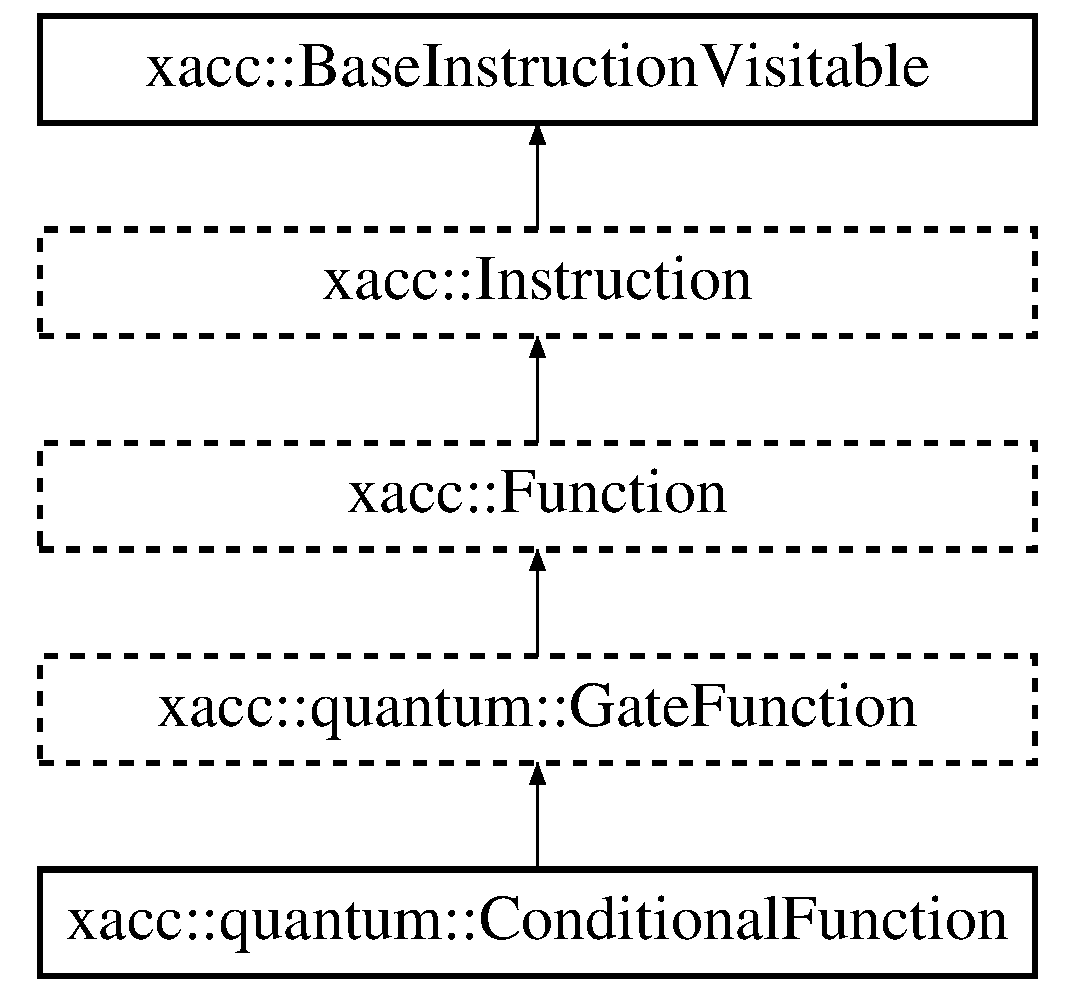
\includegraphics[height=5.000000cm]{a00025}
\end{center}
\end{figure}
\subsection*{Public Member Functions}
\begin{DoxyCompactItemize}
\item 
{\bfseries Conditional\+Function} (int qbit)\hypertarget{a00025_aa28610a08ae04d62ccdd8359433100c3}{}\label{a00025_aa28610a08ae04d62ccdd8359433100c3}

\item 
virtual void \hyperlink{a00025_a6aedad20f96390880efdc0a476b3273f}{add\+Instruction} (Inst\+Ptr instruction)
\item 
const int {\bfseries get\+Conditional\+Qubit} ()\hypertarget{a00025_a804317333b6677a041a3071b5108c0df}{}\label{a00025_a804317333b6677a041a3071b5108c0df}

\item 
void {\bfseries evaluate} (const int acc\+Bit\+State)\hypertarget{a00025_a709c236a5beb62d9a3bd5265196fb6c9}{}\label{a00025_a709c236a5beb62d9a3bd5265196fb6c9}

\item 
virtual const std\+::string \hyperlink{a00025_aca7a5f849fece6fc28a904efee9a3370}{to\+String} (const std\+::string \&buffer\+Var\+Name)
\end{DoxyCompactItemize}
\subsection*{Protected Attributes}
\begin{DoxyCompactItemize}
\item 
int {\bfseries qbit\+Idx}\hypertarget{a00025_a0310536801417c0eded28a4dea1efa44}{}\label{a00025_a0310536801417c0eded28a4dea1efa44}

\end{DoxyCompactItemize}
\subsection*{Additional Inherited Members}


\subsection{Member Function Documentation}
\index{xacc\+::quantum\+::\+Conditional\+Function@{xacc\+::quantum\+::\+Conditional\+Function}!add\+Instruction@{add\+Instruction}}
\index{add\+Instruction@{add\+Instruction}!xacc\+::quantum\+::\+Conditional\+Function@{xacc\+::quantum\+::\+Conditional\+Function}}
\subsubsection[{\texorpdfstring{add\+Instruction(\+Inst\+Ptr instruction)}{addInstruction(InstPtr instruction)}}]{\setlength{\rightskip}{0pt plus 5cm}void xacc\+::quantum\+::\+Conditional\+Function\+::add\+Instruction (
\begin{DoxyParamCaption}
\item[{Inst\+Ptr}]{instruction}
\end{DoxyParamCaption}
)\hspace{0.3cm}{\ttfamily [virtual]}}\hypertarget{a00025_a6aedad20f96390880efdc0a476b3273f}{}\label{a00025_a6aedad20f96390880efdc0a476b3273f}
Add an instruction to this quantum intermediate representation.


\begin{DoxyParams}{Parameters}
{\em instruction} & \\
\hline
\end{DoxyParams}


Reimplemented from \hyperlink{a00040_a892fb69a10f0a7cb5abdab4cca61b80a}{xacc\+::quantum\+::\+Gate\+Function}.

\index{xacc\+::quantum\+::\+Conditional\+Function@{xacc\+::quantum\+::\+Conditional\+Function}!to\+String@{to\+String}}
\index{to\+String@{to\+String}!xacc\+::quantum\+::\+Conditional\+Function@{xacc\+::quantum\+::\+Conditional\+Function}}
\subsubsection[{\texorpdfstring{to\+String(const std\+::string \&buffer\+Var\+Name)}{toString(const std::string \&bufferVarName)}}]{\setlength{\rightskip}{0pt plus 5cm}const std\+::string xacc\+::quantum\+::\+Conditional\+Function\+::to\+String (
\begin{DoxyParamCaption}
\item[{const std\+::string \&}]{buffer\+Var\+Name}
\end{DoxyParamCaption}
)\hspace{0.3cm}{\ttfamily [virtual]}}\hypertarget{a00025_aca7a5f849fece6fc28a904efee9a3370}{}\label{a00025_aca7a5f849fece6fc28a904efee9a3370}
Return an assembly-\/like string representation for this function . 
\begin{DoxyParams}{Parameters}
{\em buffer\+Var\+Name} & \\
\hline
\end{DoxyParams}
\begin{DoxyReturn}{Returns}

\end{DoxyReturn}


Reimplemented from \hyperlink{a00040_aa1950776ae84bad2d0795a0441f910e7}{xacc\+::quantum\+::\+Gate\+Function}.



The documentation for this class was generated from the following files\+:\begin{DoxyCompactItemize}
\item 
Conditional\+Function.\+hpp\item 
Conditional\+Function.\+cpp\end{DoxyCompactItemize}

\chapter{simpleini}
\label{a00026}
\hypertarget{a00026}{}
\hypertarget{a00026}{}\section{xacc\+:\+:quantum\+:\+:D\+Wave\+Vertex Class Reference}
\label{a00026}\index{xacc\+::quantum\+::\+D\+Wave\+Vertex@{xacc\+::quantum\+::\+D\+Wave\+Vertex}}


{\ttfamily \#include $<$Embedding\+Algorithm.\+hpp$>$}

Inheritance diagram for xacc\+:\+:quantum\+:\+:D\+Wave\+Vertex\+:\begin{figure}[H]
\begin{center}
\leavevmode
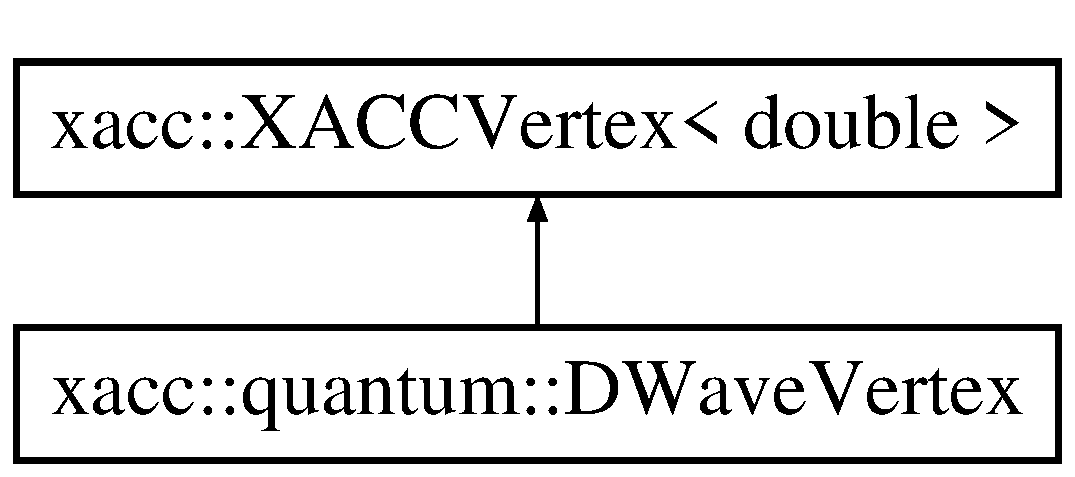
\includegraphics[height=2.000000cm]{a00026}
\end{center}
\end{figure}
\subsection*{Additional Inherited Members}


\subsection{Detailed Description}
The \hyperlink{a00026}{D\+Wave\+Vertex} is a subclass of the \hyperlink{a00073}{X\+A\+C\+C\+Vertex} that keeps track of one vertex parameter -\/ the qubit bias parameter. \hyperlink{a00073}{X\+A\+C\+C\+Vertex} already keeps track of edge weights. 

The documentation for this class was generated from the following file\+:\begin{DoxyCompactItemize}
\item 
Embedding\+Algorithm.\+hpp\end{DoxyCompactItemize}

\chapter{R\+E\+A\+D\+ME}
\label{a00027}
\hypertarget{a00027}{}
\hypertarget{a00027}{}\section{xacc\+:\+:quantum\+:\+:Embedding\+Algorithm Class Reference}
\label{a00027}\index{xacc\+::quantum\+::\+Embedding\+Algorithm@{xacc\+::quantum\+::\+Embedding\+Algorithm}}


{\ttfamily \#include $<$Embedding\+Algorithm.\+hpp$>$}

\subsection*{Public Member Functions}
\begin{DoxyCompactItemize}
\item 
\hyperlink{a00027_abad06507eef6b63af0884e3a96145c69}{Embedding\+Algorithm} ()
\item 
virtual \hyperlink{a00027_aa43660ad5d4c4b3ac67863892c33dc51}{$\sim$\+Embedding\+Algorithm} ()
\item 
virtual std\+::map$<$ int, std\+::list$<$ int $>$ $>$ \hyperlink{a00027_a67158c0f4925ff6b85698efec61e1175}{embed} (std\+::shared\+\_\+ptr$<$ \hyperlink{a00035}{D\+Wave\+Graph} $>$ problem, std\+::shared\+\_\+ptr$<$ \hyperlink{a00035}{D\+Wave\+Graph} $>$ hardware, std\+::map$<$ std\+::string, std\+::string $>$ params=std\+::map$<$ std\+::string, std\+::string $>$())=0
\item 
virtual std\+::string \hyperlink{a00027_a21079dc8ee37792977f5fd209e3f3b19}{name} ()=0
\end{DoxyCompactItemize}


\subsection{Detailed Description}
The \hyperlink{a00027}{Embedding\+Algorithm} class provides an interface for minor graph embedding algorithms. 

\subsection{Constructor \& Destructor Documentation}
\index{xacc\+::quantum\+::\+Embedding\+Algorithm@{xacc\+::quantum\+::\+Embedding\+Algorithm}!Embedding\+Algorithm@{Embedding\+Algorithm}}
\index{Embedding\+Algorithm@{Embedding\+Algorithm}!xacc\+::quantum\+::\+Embedding\+Algorithm@{xacc\+::quantum\+::\+Embedding\+Algorithm}}
\subsubsection[{\texorpdfstring{Embedding\+Algorithm()}{EmbeddingAlgorithm()}}]{\setlength{\rightskip}{0pt plus 5cm}xacc\+::quantum\+::\+Embedding\+Algorithm\+::\+Embedding\+Algorithm (
\begin{DoxyParamCaption}
{}
\end{DoxyParamCaption}
)\hspace{0.3cm}{\ttfamily [inline]}}\hypertarget{a00027_abad06507eef6b63af0884e3a96145c69}{}\label{a00027_abad06507eef6b63af0884e3a96145c69}
The Constructor \index{xacc\+::quantum\+::\+Embedding\+Algorithm@{xacc\+::quantum\+::\+Embedding\+Algorithm}!````~Embedding\+Algorithm@{$\sim$\+Embedding\+Algorithm}}
\index{````~Embedding\+Algorithm@{$\sim$\+Embedding\+Algorithm}!xacc\+::quantum\+::\+Embedding\+Algorithm@{xacc\+::quantum\+::\+Embedding\+Algorithm}}
\subsubsection[{\texorpdfstring{$\sim$\+Embedding\+Algorithm()}{~EmbeddingAlgorithm()}}]{\setlength{\rightskip}{0pt plus 5cm}virtual xacc\+::quantum\+::\+Embedding\+Algorithm\+::$\sim$\+Embedding\+Algorithm (
\begin{DoxyParamCaption}
{}
\end{DoxyParamCaption}
)\hspace{0.3cm}{\ttfamily [inline]}, {\ttfamily [virtual]}}\hypertarget{a00027_aa43660ad5d4c4b3ac67863892c33dc51}{}\label{a00027_aa43660ad5d4c4b3ac67863892c33dc51}
The Destructor 

\subsection{Member Function Documentation}
\index{xacc\+::quantum\+::\+Embedding\+Algorithm@{xacc\+::quantum\+::\+Embedding\+Algorithm}!embed@{embed}}
\index{embed@{embed}!xacc\+::quantum\+::\+Embedding\+Algorithm@{xacc\+::quantum\+::\+Embedding\+Algorithm}}
\subsubsection[{\texorpdfstring{embed(std\+::shared\+\_\+ptr$<$ D\+Wave\+Graph $>$ problem, std\+::shared\+\_\+ptr$<$ D\+Wave\+Graph $>$ hardware, std\+::map$<$ std\+::string, std\+::string $>$ params=std\+::map$<$ std\+::string, std\+::string $>$())=0}{embed(std::shared\_ptr< DWaveGraph > problem, std::shared\_ptr< DWaveGraph > hardware, std::map< std::string, std::string > params=std::map< std::string, std::string >())=0}}]{\setlength{\rightskip}{0pt plus 5cm}virtual std\+::map$<$int, std\+::list$<$int$>$ $>$ xacc\+::quantum\+::\+Embedding\+Algorithm\+::embed (
\begin{DoxyParamCaption}
\item[{std\+::shared\+\_\+ptr$<$ {\bf D\+Wave\+Graph} $>$}]{problem, }
\item[{std\+::shared\+\_\+ptr$<$ {\bf D\+Wave\+Graph} $>$}]{hardware, }
\item[{std\+::map$<$ std\+::string, std\+::string $>$}]{params = {\ttfamily std\+:\+:map$<$~std\+:\+:string,~std\+:\+:string~$>$()}}
\end{DoxyParamCaption}
)\hspace{0.3cm}{\ttfamily [pure virtual]}}\hypertarget{a00027_a67158c0f4925ff6b85698efec61e1175}{}\label{a00027_a67158c0f4925ff6b85698efec61e1175}
Implementations of \hyperlink{a00027}{Embedding\+Algorithm} implement this method to provide a valid minor graph embedding of the given problem graph into the given hardware graph.


\begin{DoxyParams}{Parameters}
{\em problem} & The problem graph to be embedded into the hardware graph \\
\hline
{\em hardware} & The hardware graph. \\
\hline
{\em params} & Any key-\/value string parameters to influence the algorithm. \\
\hline
\end{DoxyParams}
\begin{DoxyReturn}{Returns}
embedding A mapping of problem vertex indices to the list of hardware vertices they map to 
\end{DoxyReturn}
\index{xacc\+::quantum\+::\+Embedding\+Algorithm@{xacc\+::quantum\+::\+Embedding\+Algorithm}!name@{name}}
\index{name@{name}!xacc\+::quantum\+::\+Embedding\+Algorithm@{xacc\+::quantum\+::\+Embedding\+Algorithm}}
\subsubsection[{\texorpdfstring{name()=0}{name()=0}}]{\setlength{\rightskip}{0pt plus 5cm}virtual std\+::string xacc\+::quantum\+::\+Embedding\+Algorithm\+::name (
\begin{DoxyParamCaption}
{}
\end{DoxyParamCaption}
)\hspace{0.3cm}{\ttfamily [pure virtual]}}\hypertarget{a00027_a21079dc8ee37792977f5fd209e3f3b19}{}\label{a00027_a21079dc8ee37792977f5fd209e3f3b19}
Return the name of this Embedding Algorithm \begin{DoxyReturn}{Returns}

\end{DoxyReturn}


The documentation for this class was generated from the following file\+:\begin{DoxyCompactItemize}
\item 
Embedding\+Algorithm.\+hpp\end{DoxyCompactItemize}

\chapter{R\+E\+A\+D\+ME}
\label{a00028}
\hypertarget{a00028}{}
\hypertarget{a00028}{}\section{xacc\+:\+:quantum\+:\+:Chimera\+Graph Class Reference}
\label{a00028}\index{xacc\+::quantum\+::\+Chimera\+Graph@{xacc\+::quantum\+::\+Chimera\+Graph}}
Inheritance diagram for xacc\+:\+:quantum\+:\+:Chimera\+Graph\+:\begin{figure}[H]
\begin{center}
\leavevmode
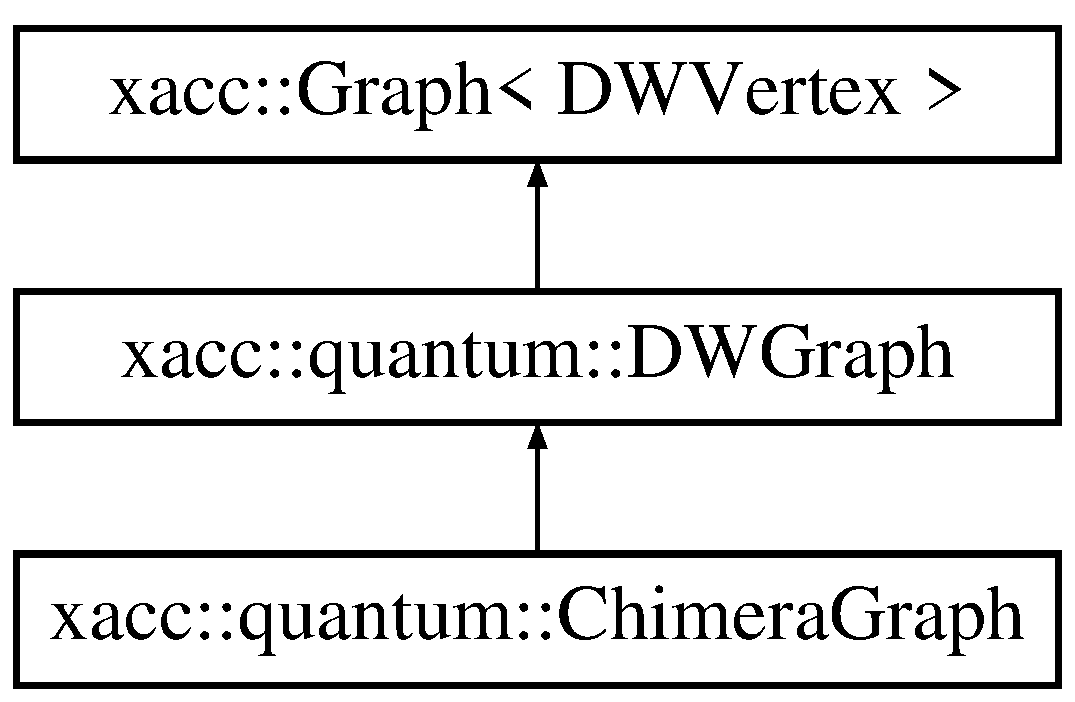
\includegraphics[height=3.000000cm]{a00028}
\end{center}
\end{figure}
\subsection*{Public Member Functions}
\begin{DoxyCompactItemize}
\item 
{\bfseries Chimera\+Graph} (int grid\+Size)\hypertarget{a00028_a64f23e464ba85d6625fe1fc2d2608052}{}\label{a00028_a64f23e464ba85d6625fe1fc2d2608052}

\end{DoxyCompactItemize}
\subsection*{Additional Inherited Members}


The documentation for this class was generated from the following file\+:\begin{DoxyCompactItemize}
\item 
D\+W\+Graph.\+hpp\end{DoxyCompactItemize}

\chapter{Module Index}
\section{Modules}
Here is a list of all modules\+:\begin{DoxyCompactList}
\item \contentsline{section}{Rapid\+J\+S\+ON error handling}{\pageref{a00832}}{}
\item \contentsline{section}{Rapid\+J\+S\+ON configuration}{\pageref{a00833}}{}
\end{DoxyCompactList}

\chapter{Namespace Index}
\section{Namespace List}
Here is a list of all documented namespaces with brief descriptions\+:\begin{DoxyCompactList}
\item\contentsline{section}{\hyperlink{a00822}{fire} }{\pageref{a00822}}{}
\item\contentsline{section}{\hyperlink{a00826}{rapidjson} \\*Main Rapid\+J\+S\+ON namespace }{\pageref{a00826}}{}
\item\contentsline{section}{\hyperlink{a00828}{Simple\+Web} }{\pageref{a00828}}{}
\end{DoxyCompactList}

\chapter{Hierarchical Index}
\section{Class Hierarchy}
This inheritance list is sorted roughly, but not completely, alphabetically\+:\begin{DoxyCompactList}
\item \contentsline{section}{xacc\+:\+:Accelerator\+Bit}{\pageref{a01095}}{}
\item \contentsline{section}{xacc\+:\+:Accelerator\+Buffer}{\pageref{a01099}}{}
\begin{DoxyCompactList}
\item \contentsline{section}{xacc\+:\+:quantum\+:\+:Simulated\+Qubits}{\pageref{a01083}}{}
\end{DoxyCompactList}
\item \contentsline{section}{xacc\+:\+:Algorithm\+Generator}{\pageref{a01119}}{}
\begin{DoxyCompactList}
\item \contentsline{section}{xacc\+:\+:quantum\+:\+:Inverse\+Q\+FT}{\pageref{a00979}}{}
\item \contentsline{section}{xacc\+:\+:quantum\+:\+:Q\+FT}{\pageref{a00983}}{}
\end{DoxyCompactList}
\item A\+S\+T\+Consumer\begin{DoxyCompactList}
\item \contentsline{section}{xacc\+:\+:quantum\+:\+:Scaffold\+A\+S\+T\+Consumer}{\pageref{a00931}}{}
\end{DoxyCompactList}
\item \contentsline{section}{xacc\+:\+:Base\+Instruction\+Visitable}{\pageref{a01147}}{}
\begin{DoxyCompactList}
\item \contentsline{section}{xacc\+:\+:Instruction}{\pageref{a01131}}{}
\begin{DoxyCompactList}
\item \contentsline{section}{xacc\+:\+:Function}{\pageref{a01127}}{}
\begin{DoxyCompactList}
\item \contentsline{section}{xacc\+:\+:quantum\+:\+:Gate\+Function}{\pageref{a00987}}{}
\begin{DoxyCompactList}
\item \contentsline{section}{xacc\+:\+:quantum\+:\+:Conditional\+Function}{\pageref{a01011}}{}
\end{DoxyCompactList}
\end{DoxyCompactList}
\item \contentsline{section}{xacc\+:\+:quantum\+:\+:Gate\+Instruction}{\pageref{a00991}}{}
\begin{DoxyCompactList}
\item \contentsline{section}{xacc\+:\+:quantum\+:\+:C\+N\+OT}{\pageref{a01007}}{}
\item \contentsline{section}{xacc\+:\+:quantum\+:\+:C\+Phase}{\pageref{a01015}}{}
\item \contentsline{section}{xacc\+:\+:quantum\+:\+:Hadamard}{\pageref{a01019}}{}
\item \contentsline{section}{xacc\+:\+:quantum\+:\+:Measure}{\pageref{a01023}}{}
\item \contentsline{section}{xacc\+:\+:quantum\+:\+:Rx}{\pageref{a01027}}{}
\item \contentsline{section}{xacc\+:\+:quantum\+:\+:Ry}{\pageref{a01031}}{}
\item \contentsline{section}{xacc\+:\+:quantum\+:\+:Rz}{\pageref{a01035}}{}
\item \contentsline{section}{xacc\+:\+:quantum\+:\+:Swap}{\pageref{a01039}}{}
\item \contentsline{section}{xacc\+:\+:quantum\+:\+:X}{\pageref{a01043}}{}
\item \contentsline{section}{xacc\+:\+:quantum\+:\+:Y}{\pageref{a01047}}{}
\item \contentsline{section}{xacc\+:\+:quantum\+:\+:Z}{\pageref{a01051}}{}
\end{DoxyCompactList}
\end{DoxyCompactList}
\end{DoxyCompactList}
\item \contentsline{section}{xacc\+:\+:Base\+Instruction\+Visitor}{\pageref{a01139}}{}
\begin{DoxyCompactList}
\item \contentsline{section}{xacc\+:\+:quantum\+:\+:All\+Gate\+Visitor}{\pageref{a01059}}{}
\begin{DoxyCompactList}
\item \contentsline{section}{xacc\+:\+:quantum\+:\+:Functional\+Gate\+Instruction\+Visitor}{\pageref{a01067}}{}
\item \contentsline{section}{xacc\+:\+:quantum\+:\+:Json\+Visitor}{\pageref{a01071}}{}
\item \contentsline{section}{xacc\+:\+:quantum\+:\+:Quil\+Visitor}{\pageref{a00915}}{}
\item \contentsline{section}{xacc\+:\+:quantum\+:\+:Scaffold\+I\+R\+To\+Src\+Visitor}{\pageref{a00939}}{}
\end{DoxyCompactList}
\item \contentsline{section}{xacc\+:\+:quantum\+:\+:Count\+Gates\+Of\+Type\+Visitor$<$ Gate\+Type $>$}{\pageref{a01063}}{}
\end{DoxyCompactList}
\item \contentsline{section}{xacc\+:\+:C\+L\+I\+Parser}{\pageref{a01163}}{}
\item \contentsline{section}{xacc\+:\+:Default\+Edge}{\pageref{a01179}}{}
\item \contentsline{section}{xacc\+:\+:quantum\+:\+:Embedding\+Algorithm}{\pageref{a00955}}{}
\item std\+:\+:exception\begin{DoxyCompactList}
\item \contentsline{section}{xacc\+:\+:X\+A\+C\+C\+Exception}{\pageref{a01243}}{}
\end{DoxyCompactList}
\item false\+\_\+type\begin{DoxyCompactList}
\item \contentsline{section}{xacc\+:\+:is\+\_\+valid\+\_\+vertex$<$ T, typename $>$}{\pageref{a01167}}{}
\end{DoxyCompactList}
\item \contentsline{section}{xacc\+:\+:Graph$<$ Vertex, type $>$}{\pageref{a01187}}{}
\item \contentsline{section}{xacc\+:\+:Graph$<$ Circuit\+Node $>$}{\pageref{a01187}}{}
\begin{DoxyCompactList}
\item \contentsline{section}{xacc\+:\+:quantum\+:\+:Gate\+Q\+IR}{\pageref{a01003}}{}
\item \contentsline{section}{xacc\+:\+:quantum\+:\+:Quantum\+Circuit}{\pageref{a01079}}{}
\end{DoxyCompactList}
\item \contentsline{section}{xacc\+:\+:Instruction\+Iterator}{\pageref{a01135}}{}
\item \contentsline{section}{xacc\+:\+:Instruction\+Visitor$<$ T $>$}{\pageref{a01143}}{}
\item \contentsline{section}{xacc\+:\+:Instruction\+Visitor$<$ C\+N\+OT $>$}{\pageref{a01143}}{}
\begin{DoxyCompactList}
\item \contentsline{section}{xacc\+:\+:quantum\+:\+:All\+Gate\+Visitor}{\pageref{a01059}}{}
\end{DoxyCompactList}
\item \contentsline{section}{xacc\+:\+:Instruction\+Visitor$<$ Conditional\+Function $>$}{\pageref{a01143}}{}
\begin{DoxyCompactList}
\item \contentsline{section}{xacc\+:\+:quantum\+:\+:All\+Gate\+Visitor}{\pageref{a01059}}{}
\end{DoxyCompactList}
\item \contentsline{section}{xacc\+:\+:Instruction\+Visitor$<$ C\+Phase $>$}{\pageref{a01143}}{}
\begin{DoxyCompactList}
\item \contentsline{section}{xacc\+:\+:quantum\+:\+:All\+Gate\+Visitor}{\pageref{a01059}}{}
\end{DoxyCompactList}
\item \contentsline{section}{xacc\+:\+:Instruction\+Visitor$<$ Gate\+Function $>$}{\pageref{a01143}}{}
\begin{DoxyCompactList}
\item \contentsline{section}{xacc\+:\+:quantum\+:\+:All\+Gate\+Visitor}{\pageref{a01059}}{}
\end{DoxyCompactList}
\item \contentsline{section}{xacc\+:\+:Instruction\+Visitor$<$ Gate\+Type $>$}{\pageref{a01143}}{}
\begin{DoxyCompactList}
\item \contentsline{section}{xacc\+:\+:quantum\+:\+:Count\+Gates\+Of\+Type\+Visitor$<$ Gate\+Type $>$}{\pageref{a01063}}{}
\end{DoxyCompactList}
\item \contentsline{section}{xacc\+:\+:Instruction\+Visitor$<$ Hadamard $>$}{\pageref{a01143}}{}
\begin{DoxyCompactList}
\item \contentsline{section}{xacc\+:\+:quantum\+:\+:All\+Gate\+Visitor}{\pageref{a01059}}{}
\end{DoxyCompactList}
\item \contentsline{section}{xacc\+:\+:Instruction\+Visitor$<$ Measure $>$}{\pageref{a01143}}{}
\begin{DoxyCompactList}
\item \contentsline{section}{xacc\+:\+:quantum\+:\+:All\+Gate\+Visitor}{\pageref{a01059}}{}
\end{DoxyCompactList}
\item \contentsline{section}{xacc\+:\+:Instruction\+Visitor$<$ Rx $>$}{\pageref{a01143}}{}
\begin{DoxyCompactList}
\item \contentsline{section}{xacc\+:\+:quantum\+:\+:All\+Gate\+Visitor}{\pageref{a01059}}{}
\end{DoxyCompactList}
\item \contentsline{section}{xacc\+:\+:Instruction\+Visitor$<$ Ry $>$}{\pageref{a01143}}{}
\begin{DoxyCompactList}
\item \contentsline{section}{xacc\+:\+:quantum\+:\+:All\+Gate\+Visitor}{\pageref{a01059}}{}
\end{DoxyCompactList}
\item \contentsline{section}{xacc\+:\+:Instruction\+Visitor$<$ Rz $>$}{\pageref{a01143}}{}
\begin{DoxyCompactList}
\item \contentsline{section}{xacc\+:\+:quantum\+:\+:All\+Gate\+Visitor}{\pageref{a01059}}{}
\end{DoxyCompactList}
\item \contentsline{section}{xacc\+:\+:Instruction\+Visitor$<$ Swap $>$}{\pageref{a01143}}{}
\begin{DoxyCompactList}
\item \contentsline{section}{xacc\+:\+:quantum\+:\+:All\+Gate\+Visitor}{\pageref{a01059}}{}
\end{DoxyCompactList}
\item \contentsline{section}{xacc\+:\+:Instruction\+Visitor$<$ X $>$}{\pageref{a01143}}{}
\begin{DoxyCompactList}
\item \contentsline{section}{xacc\+:\+:quantum\+:\+:All\+Gate\+Visitor}{\pageref{a01059}}{}
\end{DoxyCompactList}
\item \contentsline{section}{xacc\+:\+:Instruction\+Visitor$<$ Y $>$}{\pageref{a01143}}{}
\begin{DoxyCompactList}
\item \contentsline{section}{xacc\+:\+:quantum\+:\+:All\+Gate\+Visitor}{\pageref{a01059}}{}
\end{DoxyCompactList}
\item \contentsline{section}{xacc\+:\+:Instruction\+Visitor$<$ Z $>$}{\pageref{a01143}}{}
\begin{DoxyCompactList}
\item \contentsline{section}{xacc\+:\+:quantum\+:\+:All\+Gate\+Visitor}{\pageref{a01059}}{}
\end{DoxyCompactList}
\item \contentsline{section}{xacc\+:\+:int\+\_\+$<$ size\+\_\+t $>$}{\pageref{a01183}}{}
\item \contentsline{section}{xacc\+:\+:IR}{\pageref{a01151}}{}
\begin{DoxyCompactList}
\item \contentsline{section}{xacc\+:\+:quantum\+:\+:D\+Wave\+IR}{\pageref{a00963}}{}
\item \contentsline{section}{xacc\+:\+:quantum\+:\+:Gate\+Q\+IR}{\pageref{a01003}}{}
\end{DoxyCompactList}
\item \contentsline{section}{xacc\+:\+:I\+R\+Transformation}{\pageref{a01155}}{}
\item std\+:\+:map$<$ K, T $>$\begin{DoxyCompactList}
\item \contentsline{section}{xacc\+:\+:Runtime\+Options}{\pageref{a01203}}{}
\end{DoxyCompactList}
\item \contentsline{section}{xacc\+:\+:Options\+Provider}{\pageref{a01195}}{}
\begin{DoxyCompactList}
\item \contentsline{section}{xacc\+:\+:Accelerator}{\pageref{a01087}}{}
\begin{DoxyCompactList}
\item \contentsline{section}{xacc\+:\+:quantum\+:\+:Rigetti\+Accelerator}{\pageref{a00919}}{}
\item \contentsline{section}{xacc\+:\+:quantum\+:\+:Simple\+Accelerator}{\pageref{a00943}}{}
\end{DoxyCompactList}
\item \contentsline{section}{xacc\+:\+:Compiler}{\pageref{a01103}}{}
\begin{DoxyCompactList}
\item \contentsline{section}{xacc\+:\+:quantum\+:\+:D\+Wave\+Compiler}{\pageref{a00947}}{}
\item \contentsline{section}{xacc\+:\+:quantum\+:\+:Quil\+Compiler}{\pageref{a00911}}{}
\item \contentsline{section}{xacc\+:\+:quantum\+:\+:Scaffold\+Compiler}{\pageref{a00935}}{}
\end{DoxyCompactList}
\item \contentsline{section}{xacc\+:\+:Preprocessor}{\pageref{a01111}}{}
\begin{DoxyCompactList}
\item \contentsline{section}{xacc\+:\+:quantum\+:\+:Kernel\+Replacement\+Preprocessor}{\pageref{a00967}}{}
\end{DoxyCompactList}
\end{DoxyCompactList}
\item \contentsline{section}{xacc\+:\+:Program}{\pageref{a01159}}{}
\item \contentsline{section}{xacc\+:\+:quantum\+:\+:Qasm\+To\+Graph}{\pageref{a01075}}{}
\item Recursive\+A\+S\+T\+Visitor\begin{DoxyCompactList}
\item \contentsline{section}{xacc\+:\+:quantum\+:\+:Scaffold\+A\+S\+T\+Consumer}{\pageref{a00931}}{}
\end{DoxyCompactList}
\item \contentsline{section}{xacc\+:\+:Register\+Accelerator$<$ T $>$}{\pageref{a01091}}{}
\item \contentsline{section}{xacc\+:\+:Register\+Algorithm\+Generator$<$ T $>$}{\pageref{a01123}}{}
\item \contentsline{section}{xacc\+:\+:Register\+Compiler$<$ T $>$}{\pageref{a01107}}{}
\item \contentsline{section}{xacc\+:\+:quantum\+:\+:Register\+Embedding\+Algorithm$<$ T $>$}{\pageref{a00959}}{}
\item \contentsline{section}{xacc\+:\+:quantum\+:\+:Register\+Gate\+Instruction$<$ T $>$}{\pageref{a00995}}{}
\item \contentsline{section}{xacc\+:\+:Register\+Preprocessor$<$ T $>$}{\pageref{a01115}}{}
\item \contentsline{section}{xacc\+:\+:runtime\+\_\+get\+\_\+func\+\_\+table$<$ Tuple, Indices $>$}{\pageref{a01235}}{}
\item \contentsline{section}{xacc\+:\+:runtime\+\_\+get\+\_\+func\+\_\+table$<$ Tuple, std\+:\+:index\+\_\+sequence$<$ Indices... $>$ $>$}{\pageref{a01239}}{}
\item \contentsline{section}{xacc\+:\+:Singleton$<$ T $>$}{\pageref{a01207}}{}
\item \contentsline{section}{xacc\+:\+:Singleton$<$ Registry$<$ T, T\+Args... $>$ $>$}{\pageref{a01207}}{}
\begin{DoxyCompactList}
\item \contentsline{section}{xacc\+:\+:Registry$<$ T, T\+Args... $>$}{\pageref{a01199}}{}
\item \contentsline{section}{xacc\+:\+:Registry$<$ T, T\+Args $>$}{\pageref{a01199}}{}
\end{DoxyCompactList}
\item \contentsline{section}{xacc\+:\+:Singleton$<$ Runtime\+Options $>$}{\pageref{a01207}}{}
\begin{DoxyCompactList}
\item \contentsline{section}{xacc\+:\+:Runtime\+Options}{\pageref{a01203}}{}
\end{DoxyCompactList}
\item true\+\_\+type\begin{DoxyCompactList}
\item \contentsline{section}{xacc\+:\+:is\+\_\+valid\+\_\+vertex$<$ T, decltype(std\+:\+:declval$<$ T $>$().properties, void())$>$}{\pageref{a01171}}{}
\end{DoxyCompactList}
\item \contentsline{section}{xacc\+:\+:X\+A\+C\+C\+InfoT}{\pageref{a01247}}{}
\item \contentsline{section}{xacc\+:\+:X\+A\+C\+C\+Vertex$<$ Properties $>$}{\pageref{a01175}}{}
\item \contentsline{section}{xacc\+:\+:X\+A\+C\+C\+Vertex$<$ double $>$}{\pageref{a01175}}{}
\begin{DoxyCompactList}
\item \contentsline{section}{xacc\+:\+:quantum\+:\+:D\+Wave\+Vertex}{\pageref{a00951}}{}
\end{DoxyCompactList}
\item \contentsline{section}{xacc\+:\+:X\+A\+C\+C\+Vertex$<$ std\+:\+:string $>$}{\pageref{a01175}}{}
\item \contentsline{section}{xacc\+:\+:X\+A\+C\+C\+Vertex$<$ std\+:\+:string, double, int, float $>$}{\pageref{a01175}}{}
\item \contentsline{section}{xacc\+:\+:X\+A\+C\+C\+Vertex$<$ std\+:\+:string, int, int, std\+:\+:vector$<$ int $>$, bool, std\+:\+:vector$<$ std\+:\+:string $>$ $>$}{\pageref{a01175}}{}
\begin{DoxyCompactList}
\item \contentsline{section}{xacc\+:\+:quantum\+:\+:Circuit\+Node}{\pageref{a00999}}{}
\item \contentsline{section}{xacc\+:\+:quantum\+:\+:Circuit\+Node}{\pageref{a00999}}{}
\end{DoxyCompactList}
\item \contentsline{section}{xacc\+:\+:X\+A\+C\+C\+Vertex$<$ std\+:\+:vector$<$ int $>$ $>$}{\pageref{a01175}}{}
\item \contentsline{section}{xacc\+:\+:Graph$<$ Vertex, type $>$\+:\+:X\+A\+C\+C\+Vertex\+Properties\+Writer}{\pageref{a01191}}{}
\end{DoxyCompactList}

\chapter{Class Index}
\section{Class List}
Here are the classes, structs, unions and interfaces with brief descriptions\+:\begin{DoxyCompactList}
\item\contentsline{section}{\hyperlink{a00011}{xacc\+::\+Accelerator} }{\pageref{a00011}}{}
\item\contentsline{section}{\hyperlink{a00012}{Accelerator\+Bit} }{\pageref{a00012}}{}
\item\contentsline{section}{\hyperlink{a00013}{Accelerator\+Buffer} }{\pageref{a00013}}{}
\item\contentsline{section}{\hyperlink{a00014}{xacc\+::quantum\+::\+All\+Gate\+Visitor} }{\pageref{a00014}}{}
\item\contentsline{section}{\hyperlink{a00015}{xacc\+::\+Base\+Instruction\+Visitable} }{\pageref{a00015}}{}
\item\contentsline{section}{\hyperlink{a00016}{xacc\+::\+Base\+Instruction\+Visitor} }{\pageref{a00016}}{}
\item\contentsline{section}{\hyperlink{a00017}{xacc\+::quantum\+::\+Circuit\+Node} }{\pageref{a00017}}{}
\item\contentsline{section}{\hyperlink{a00018}{xacc\+::\+C\+L\+I\+Parser} }{\pageref{a00018}}{}
\item\contentsline{section}{\hyperlink{a00019}{xacc\+::quantum\+::\+C\+N\+OT} }{\pageref{a00019}}{}
\item\contentsline{section}{\hyperlink{a00020}{xacc\+::\+Compiler} }{\pageref{a00020}}{}
\item\contentsline{section}{\hyperlink{a00021}{xacc\+::quantum\+::\+Conditional\+Function} }{\pageref{a00021}}{}
\item\contentsline{section}{\hyperlink{a00022}{Count\+Gate\+Visitor$<$ Gate\+Type $>$} }{\pageref{a00022}}{}
\item\contentsline{section}{\hyperlink{a00023}{xacc\+::\+Default\+Edge} }{\pageref{a00023}}{}
\item\contentsline{section}{\hyperlink{a00024}{xacc\+::quantum\+::\+D\+Wave\+Compiler} }{\pageref{a00024}}{}
\item\contentsline{section}{\hyperlink{a00025}{xacc\+::quantum\+::\+D\+Wave\+IR} }{\pageref{a00025}}{}
\item\contentsline{section}{\hyperlink{a00026}{xacc\+::quantum\+::\+D\+Wave\+Vertex} }{\pageref{a00026}}{}
\item\contentsline{section}{\hyperlink{a00027}{xacc\+::quantum\+::\+Embedding\+Algorithm} }{\pageref{a00027}}{}
\item\contentsline{section}{\hyperlink{a00028}{F} }{\pageref{a00028}}{}
\item\contentsline{section}{\hyperlink{a00029}{Fake\+Http\+Client} }{\pageref{a00029}}{}
\item\contentsline{section}{\hyperlink{a00030}{xacc\+::\+Function} }{\pageref{a00030}}{}
\item\contentsline{section}{\hyperlink{a00031}{xacc\+::quantum\+::\+Functional\+Gate\+Instruction\+Visitor} }{\pageref{a00031}}{}
\item\contentsline{section}{\hyperlink{a00032}{xacc\+::quantum\+::\+Gate\+Function} }{\pageref{a00032}}{}
\item\contentsline{section}{\hyperlink{a00033}{xacc\+::quantum\+::\+Gate\+Instruction} }{\pageref{a00033}}{}
\item\contentsline{section}{\hyperlink{a00034}{xacc\+::quantum\+::\+Gate\+Q\+IR} }{\pageref{a00034}}{}
\item\contentsline{section}{\hyperlink{a00035}{xacc\+::\+Graph$<$ Vertex, type $>$} }{\pageref{a00035}}{}
\item\contentsline{section}{\hyperlink{a00036}{xacc\+::quantum\+::\+Hadamard} }{\pageref{a00036}}{}
\item\contentsline{section}{\hyperlink{a00037}{xacc\+::\+Instruction} }{\pageref{a00037}}{}
\item\contentsline{section}{\hyperlink{a00038}{xacc\+::\+Instruction\+Iterator} }{\pageref{a00038}}{}
\item\contentsline{section}{\hyperlink{a00039}{xacc\+::\+Instruction\+Visitor$<$ T $>$} }{\pageref{a00039}}{}
\item\contentsline{section}{\hyperlink{a00040}{xacc\+::int\+\_\+$<$ size\+\_\+t $>$} }{\pageref{a00040}}{}
\item\contentsline{section}{\hyperlink{a00041}{xacc\+::\+IR} }{\pageref{a00041}}{}
\item\contentsline{section}{\hyperlink{a00042}{xacc\+::\+I\+R\+Transformation} }{\pageref{a00042}}{}
\item\contentsline{section}{\hyperlink{a00043}{xacc\+::is\+\_\+valid\+\_\+vertex$<$ T, typename $>$} }{\pageref{a00043}}{}
\item\contentsline{section}{\hyperlink{a00044}{xacc\+::quantum\+::\+Json\+Visitor} }{\pageref{a00044}}{}
\item\contentsline{section}{\hyperlink{a00045}{xacc\+::quantum\+::\+Measure} }{\pageref{a00045}}{}
\item\contentsline{section}{\hyperlink{a00046}{xacc\+::\+Options\+Provider} }{\pageref{a00046}}{}
\item\contentsline{section}{\hyperlink{a00047}{xacc\+::\+Program} }{\pageref{a00047}}{}
\item\contentsline{section}{\hyperlink{a00048}{xacc\+::quantum\+::\+Qasm\+To\+Graph} }{\pageref{a00048}}{}
\item\contentsline{section}{\hyperlink{a00049}{xacc\+::quantum\+::\+Quantum\+Circuit} }{\pageref{a00049}}{}
\item\contentsline{section}{\hyperlink{a00050}{xacc\+::quantum\+::\+Quil\+Compiler} }{\pageref{a00050}}{}
\item\contentsline{section}{\hyperlink{a00051}{xacc\+::quantum\+::\+Quil\+Visitor} }{\pageref{a00051}}{}
\item\contentsline{section}{\hyperlink{a00052}{xacc\+::\+Register\+Accelerator$<$ T $>$} }{\pageref{a00052}}{}
\item\contentsline{section}{\hyperlink{a00053}{xacc\+::\+Register\+Compiler$<$ T $>$} }{\pageref{a00053}}{}
\item\contentsline{section}{\hyperlink{a00054}{xacc\+::quantum\+::\+Register\+Embedding\+Algorithm$<$ T $>$} }{\pageref{a00054}}{}
\item\contentsline{section}{\hyperlink{a00055}{xacc\+::quantum\+::\+Register\+Gate\+Instruction$<$ T $>$} }{\pageref{a00055}}{}
\item\contentsline{section}{\hyperlink{a00056}{xacc\+::\+Registry$<$ T, T\+Args $>$} }{\pageref{a00056}}{}
\item\contentsline{section}{\hyperlink{a00057}{xacc\+::quantum\+::\+Rigetti\+Accelerator} }{\pageref{a00057}}{}
\item\contentsline{section}{\hyperlink{a00058}{xacc\+::runtime\+\_\+get\+\_\+func\+\_\+table$<$ Tuple, Indices $>$} }{\pageref{a00058}}{}
\item\contentsline{section}{\hyperlink{a00059}{xacc\+::runtime\+\_\+get\+\_\+func\+\_\+table$<$ Tuple, std\+::index\+\_\+sequence$<$ Indices... $>$ $>$} }{\pageref{a00059}}{}
\item\contentsline{section}{\hyperlink{a00060}{xacc\+::\+Runtime\+Options} }{\pageref{a00060}}{}
\item\contentsline{section}{\hyperlink{a00061}{xacc\+::quantum\+::\+Rx} }{\pageref{a00061}}{}
\item\contentsline{section}{\hyperlink{a00062}{xacc\+::quantum\+::\+Ry} }{\pageref{a00062}}{}
\item\contentsline{section}{\hyperlink{a00063}{xacc\+::quantum\+::\+Rz} }{\pageref{a00063}}{}
\item\contentsline{section}{\hyperlink{a00064}{scaffold\+::\+Scaffold\+A\+S\+T\+Consumer} }{\pageref{a00064}}{}
\item\contentsline{section}{\hyperlink{a00065}{xacc\+::quantum\+::\+Scaffold\+Compiler} }{\pageref{a00065}}{}
\item\contentsline{section}{\hyperlink{a00066}{xacc\+::quantum\+::\+Simple\+Accelerator} }{\pageref{a00066}}{}
\item\contentsline{section}{\hyperlink{a00067}{xacc\+::quantum\+::\+Simulated\+Qubits$<$ Total\+Number\+Of\+Qubits $>$} }{\pageref{a00067}}{}
\item\contentsline{section}{\hyperlink{a00068}{xacc\+::\+Singleton$<$ T $>$} }{\pageref{a00068}}{}
\item\contentsline{section}{\hyperlink{a00069}{Test\+Visitor} }{\pageref{a00069}}{}
\item\contentsline{section}{\hyperlink{a00070}{xacc\+::quantum\+::X} }{\pageref{a00070}}{}
\item\contentsline{section}{\hyperlink{a00071}{xacc\+::\+X\+A\+C\+C\+Exception} }{\pageref{a00071}}{}
\item\contentsline{section}{\hyperlink{a00072}{xacc\+::\+X\+A\+C\+C\+InfoT} }{\pageref{a00072}}{}
\item\contentsline{section}{\hyperlink{a00073}{xacc\+::\+X\+A\+C\+C\+Vertex$<$ Properties $>$} }{\pageref{a00073}}{}
\item\contentsline{section}{\hyperlink{a00074}{xacc\+::\+Graph$<$ Vertex, type $>$\+::\+X\+A\+C\+C\+Vertex\+Properties\+Writer} }{\pageref{a00074}}{}
\item\contentsline{section}{\hyperlink{a00075}{xacc\+::quantum\+::Y} }{\pageref{a00075}}{}
\item\contentsline{section}{\hyperlink{a00076}{xacc\+::quantum\+::Z} }{\pageref{a00076}}{}
\end{DoxyCompactList}

\chapter{File Index}
\section{File List}
Here is a list of all documented files with brief descriptions\+:\begin{DoxyCompactList}
\item\contentsline{section}{{\bfseries Accelerator.\+hpp} }{\pageref{a00578}}{}
\item\contentsline{section}{{\bfseries Accelerator\+Buffer.\+hpp} }{\pageref{a00581}}{}
\item\contentsline{section}{{\bfseries aggressive\+\_\+ptr\+\_\+cast.\+hpp} }{\pageref{a00203}}{}
\item\contentsline{section}{\hyperlink{a00200}{alias.\+hpp} \\*Includes alias methods and macro. You can include this header or \hyperlink{a00269}{boost/dll/shared\+\_\+library.\+hpp} to reduce dependencies in case you do not use the refcountable functions }{\pageref{a00200}}{}
\item\contentsline{section}{{\bfseries All\+Gate\+Visitor.\+hpp} }{\pageref{a00176}}{}
\item\contentsline{section}{{\bfseries allocators.\+h} }{\pageref{a00473}}{}
\item\contentsline{section}{{\bfseries Asio\+Networking\+Tool.\+hpp} }{\pageref{a00464}}{}
\item\contentsline{section}{{\bfseries biginteger.\+h} }{\pageref{a00500}}{}
\item\contentsline{section}{{\bfseries build.\+h} }{\pageref{a00365}}{}
\item\contentsline{section}{{\bfseries client\+\_\+http.\+hpp} }{\pageref{a00452}}{}
\item\contentsline{section}{{\bfseries client\+\_\+https.\+hpp} }{\pageref{a00455}}{}
\item\contentsline{section}{{\bfseries C\+L\+I\+Parser.\+hpp} }{\pageref{a00611}}{}
\item\contentsline{section}{{\bfseries C\+N\+O\+T.\+hpp} }{\pageref{a00104}}{}
\item\contentsline{section}{{\bfseries Compiler.\+hpp} }{\pageref{a00584}}{}
\item\contentsline{section}{{\bfseries Conditional\+Function.\+hpp} }{\pageref{a00110}}{}
\item\contentsline{section}{{\bfseries Convert\+U\+T\+F.\+h} }{\pageref{a00437}}{}
\item\contentsline{section}{{\bfseries ctor\+\_\+dtor.\+hpp} }{\pageref{a00206}}{}
\item\contentsline{section}{{\bfseries Delimited\+Text\+Parser.\+h} }{\pageref{a00368}}{}
\item\contentsline{section}{{\bfseries demangle\+\_\+symbol.\+hpp} }{\pageref{a00209}}{}
\item\contentsline{section}{{\bfseries diyfp.\+h} }{\pageref{a00503}}{}
\item\contentsline{section}{\hyperlink{a00278}{dll.\+hpp} \\*Includes all the non-\/experimental headers of the Boost.\+D\+LL library }{\pageref{a00278}}{}
\item\contentsline{section}{\hyperlink{a00476}{document.\+h} }{\pageref{a00476}}{}
\item\contentsline{section}{{\bfseries dtoa.\+h} }{\pageref{a00506}}{}
\item\contentsline{section}{{\bfseries D\+Wave\+Compiler.\+hpp} }{\pageref{a00077}}{}
\item\contentsline{section}{{\bfseries D\+Wave\+I\+R.\+hpp} }{\pageref{a00086}}{}
\item\contentsline{section}{{\bfseries Eigen\+Tensor\+Provider.\+hpp} }{\pageref{a00416}}{}
\item\contentsline{section}{{\bfseries elf\+\_\+info.\+hpp} }{\pageref{a00221}}{}
\item\contentsline{section}{{\bfseries Embedding\+Algorithm.\+hpp} }{\pageref{a00080}}{}
\item\contentsline{section}{{\bfseries en.\+h} }{\pageref{a00485}}{}
\item\contentsline{section}{{\bfseries encodedstream.\+h} }{\pageref{a00479}}{}
\item\contentsline{section}{{\bfseries encodings.\+h} }{\pageref{a00482}}{}
\item\contentsline{section}{\hyperlink{a00488}{error.\+h} }{\pageref{a00488}}{}
\item\contentsline{section}{{\bfseries filereadstream.\+h} }{\pageref{a00491}}{}
\item\contentsline{section}{{\bfseries filewritestream.\+h} }{\pageref{a00494}}{}
\item\contentsline{section}{{\bfseries Function.\+hpp} }{\pageref{a00587}}{}
\item\contentsline{section}{{\bfseries Functional\+Gate\+Instruction\+Visitor.\+hpp} }{\pageref{a00056}}{}
\item\contentsline{section}{{\bfseries fwd.\+h} }{\pageref{a00497}}{}
\item\contentsline{section}{{\bfseries Gate\+Function.\+hpp} }{\pageref{a00089}}{}
\item\contentsline{section}{{\bfseries Gate\+Instruction.\+hpp} }{\pageref{a00092}}{}
\item\contentsline{section}{{\bfseries Gate\+Q\+I\+R.\+hpp} }{\pageref{a00098}}{}
\item\contentsline{section}{{\bfseries get\+\_\+mem\+\_\+fn\+\_\+type.\+hpp} }{\pageref{a00224}}{}
\item\contentsline{section}{{\bfseries Graph.\+hpp} }{\pageref{a00614}}{}
\item\contentsline{section}{{\bfseries Hadamard.\+hpp} }{\pageref{a00116}}{}
\item\contentsline{section}{{\bfseries ieee754.\+h} }{\pageref{a00509}}{}
\item\contentsline{section}{{\bfseries I\+Local\+Parser.\+h} }{\pageref{a00371}}{}
\item\contentsline{section}{\hyperlink{a00254}{import.\+hpp} \\*Contains all the boost\+::dll\+::import$\ast$ reference counting functions that hold a shared pointer to the instance of \hyperlink{a01708}{boost\+::dll\+::shared\+\_\+library} }{\pageref{a00254}}{}
\item\contentsline{section}{{\bfseries import\+\_\+class.\+hpp} }{\pageref{a00257}}{}
\item\contentsline{section}{{\bfseries import\+\_\+mangled.\+hpp} }{\pageref{a00260}}{}
\item\contentsline{section}{{\bfseries import\+\_\+mangled\+\_\+helpers.\+hpp} }{\pageref{a00227}}{}
\item\contentsline{section}{{\bfseries I\+Networking\+Tool.\+hpp} }{\pageref{a00467}}{}
\item\contentsline{section}{{\bfseries I\+N\+I\+Property\+Parser.\+h} }{\pageref{a00374}}{}
\item\contentsline{section}{{\bfseries Instruction.\+hpp} }{\pageref{a00590}}{}
\item\contentsline{section}{{\bfseries Instruction\+Iterator.\+hpp} }{\pageref{a00593}}{}
\item\contentsline{section}{{\bfseries Instruction\+Visitor.\+hpp} }{\pageref{a00596}}{}
\item\contentsline{section}{{\bfseries inttypes.\+h} }{\pageref{a00545}}{}
\item\contentsline{section}{{\bfseries I\+Parser.\+h} }{\pageref{a00377}}{}
\item\contentsline{section}{{\bfseries I\+Property\+Parser.\+h} }{\pageref{a00380}}{}
\item\contentsline{section}{{\bfseries I\+R.\+hpp} }{\pageref{a00599}}{}
\item\contentsline{section}{{\bfseries I\+R\+Transformation.\+hpp} }{\pageref{a00602}}{}
\item\contentsline{section}{{\bfseries I\+Stepper.\+h} }{\pageref{a00356}}{}
\item\contentsline{section}{{\bfseries istreamwrapper.\+h} }{\pageref{a00536}}{}
\item\contentsline{section}{{\bfseries itanium.\+hpp} }{\pageref{a00212}}{}
\item\contentsline{section}{{\bfseries itoa.\+h} }{\pageref{a00512}}{}
\item\contentsline{section}{{\bfseries Json\+Visitor.\+hpp} }{\pageref{a00179}}{}
\item\contentsline{section}{\hyperlink{a00263}{library\+\_\+info.\+hpp} \\*Contains only the \hyperlink{a01704}{boost\+::dll\+::library\+\_\+info} class that is capable of extracting different information from binaries }{\pageref{a00263}}{}
\item\contentsline{section}{{\bfseries Local\+Parser.\+h} }{\pageref{a00383}}{}
\item\contentsline{section}{{\bfseries macho\+\_\+info.\+hpp} }{\pageref{a00230}}{}
\item\contentsline{section}{{\bfseries mangled\+\_\+storage\+\_\+base.\+hpp} }{\pageref{a00215}}{}
\item\contentsline{section}{{\bfseries Measure.\+hpp} }{\pageref{a00122}}{}
\item\contentsline{section}{{\bfseries memorybuffer.\+h} }{\pageref{a00539}}{}
\item\contentsline{section}{{\bfseries memorystream.\+h} }{\pageref{a00542}}{}
\item\contentsline{section}{{\bfseries meta.\+h} }{\pageref{a00515}}{}
\item\contentsline{section}{{\bfseries msvc.\+hpp} }{\pageref{a00218}}{}
\item\contentsline{section}{{\bfseries O\+D\+E\+Solver.\+h} }{\pageref{a00404}}{}
\item\contentsline{section}{{\bfseries Options\+Provider.\+hpp} }{\pageref{a00617}}{}
\item\contentsline{section}{{\bfseries ostreamwrapper.\+h} }{\pageref{a00551}}{}
\item\contentsline{section}{{\bfseries parse.\+h} }{\pageref{a00386}}{}
\item\contentsline{section}{{\bfseries posix/path\+\_\+from\+\_\+handle.\+hpp} }{\pageref{a03082}}{}
\item\contentsline{section}{{\bfseries windows/path\+\_\+from\+\_\+handle.\+hpp} }{\pageref{a03085}}{}
\item\contentsline{section}{{\bfseries pe\+\_\+info.\+hpp} }{\pageref{a00233}}{}
\item\contentsline{section}{{\bfseries pointer.\+h} }{\pageref{a00554}}{}
\item\contentsline{section}{{\bfseries pow10.\+h} }{\pageref{a00518}}{}
\item\contentsline{section}{{\bfseries prettywriter.\+h} }{\pageref{a00557}}{}
\item\contentsline{section}{{\bfseries Profile\+Stepper.\+h} }{\pageref{a00359}}{}
\item\contentsline{section}{{\bfseries Program.\+hpp} }{\pageref{a00605}}{}
\item\contentsline{section}{{\bfseries program\+\_\+location\+\_\+impl.\+hpp} }{\pageref{a00239}}{}
\item\contentsline{section}{{\bfseries Qasm\+To\+Graph.\+hpp} }{\pageref{a00182}}{}
\item\contentsline{section}{{\bfseries Quantum\+Circuit.\+hpp} }{\pageref{a00185}}{}
\item\contentsline{section}{{\bfseries Quil\+Compiler.\+hpp} }{\pageref{a00020}}{}
\item\contentsline{section}{{\bfseries Quil\+Visitor.\+hpp} }{\pageref{a00023}}{}
\item\contentsline{section}{\hyperlink{a00560}{rapidjson.\+h} \\*Common definitions and configuration }{\pageref{a00560}}{}
\item\contentsline{section}{{\bfseries Reaction.\+h} }{\pageref{a00281}}{}
\item\contentsline{section}{{\bfseries Reaction\+Local\+Parser.\+h} }{\pageref{a00284}}{}
\item\contentsline{section}{{\bfseries Reaction\+Network.\+h} }{\pageref{a00287}}{}
\item\contentsline{section}{\hyperlink{a00563}{reader.\+h} }{\pageref{a00563}}{}
\item\contentsline{section}{{\bfseries regex.\+h} }{\pageref{a00521}}{}
\item\contentsline{section}{{\bfseries Registry.\+hpp} }{\pageref{a00620}}{}
\item\contentsline{section}{{\bfseries Rigetti\+Accelerator.\+hpp} }{\pageref{a00029}}{}
\item\contentsline{section}{\hyperlink{a00266}{runtime\+\_\+symbol\+\_\+info.\+hpp} \\*Provides methods for getting acceptable by \hyperlink{a01708}{boost\+::dll\+::shared\+\_\+library} location of symbol, source line or program }{\pageref{a00266}}{}
\item\contentsline{section}{{\bfseries Runtime\+Options.\+hpp} }{\pageref{a00623}}{}
\item\contentsline{section}{{\bfseries Rz.\+hpp} }{\pageref{a00128}}{}
\item\contentsline{section}{{\bfseries Scaffold\+A\+S\+T\+Consumer.\+hpp} }{\pageref{a00041}}{}
\item\contentsline{section}{{\bfseries Scaffold\+Compiler.\+hpp} }{\pageref{a00047}}{}
\item\contentsline{section}{{\bfseries schema.\+h} }{\pageref{a00566}}{}
\item\contentsline{section}{{\bfseries server\+\_\+http.\+hpp} }{\pageref{a00458}}{}
\item\contentsline{section}{{\bfseries server\+\_\+https.\+hpp} }{\pageref{a00461}}{}
\item\contentsline{section}{\hyperlink{a00269}{shared\+\_\+library.\+hpp} \\*Contains the \hyperlink{a01708}{boost\+::dll\+::shared\+\_\+library} class, core class for all the D\+L\+L/\+D\+SO operations }{\pageref{a00269}}{}
\item\contentsline{section}{{\bfseries posix/shared\+\_\+library\+\_\+impl.\+hpp} }{\pageref{a03130}}{}
\item\contentsline{section}{{\bfseries windows/shared\+\_\+library\+\_\+impl.\+hpp} }{\pageref{a03133}}{}
\item\contentsline{section}{\hyperlink{a00272}{shared\+\_\+library\+\_\+load\+\_\+mode.\+hpp} \\*Contains only the boost\+::dll\+::load\+\_\+mode\+::type enum and operators related to it }{\pageref{a00272}}{}
\item\contentsline{section}{{\bfseries Simple\+Accelerator.\+hpp} }{\pageref{a00062}}{}
\item\contentsline{section}{{\bfseries Simple\+Ini.\+h} }{\pageref{a00440}}{}
\item\contentsline{section}{{\bfseries Simulated\+Qubits.\+hpp} }{\pageref{a00065}}{}
\item\contentsline{section}{{\bfseries Singleton.\+hpp} }{\pageref{a00626}}{}
\item\contentsline{section}{\hyperlink{a00275}{smart\+\_\+library.\+hpp} \\*Contains the \hyperlink{a01712}{boost\+::dll\+::experimental\+::smart\+\_\+library} class for loading mangled symbols }{\pageref{a00275}}{}
\item\contentsline{section}{{\bfseries Species.\+h} }{\pageref{a00290}}{}
\item\contentsline{section}{{\bfseries Species\+Local\+Parser.\+h} }{\pageref{a00293}}{}
\item\contentsline{section}{{\bfseries stack.\+h} }{\pageref{a00524}}{}
\item\contentsline{section}{{\bfseries stdint.\+h} }{\pageref{a00548}}{}
\item\contentsline{section}{{\bfseries stream.\+h} }{\pageref{a00569}}{}
\item\contentsline{section}{{\bfseries strfunc.\+h} }{\pageref{a00527}}{}
\item\contentsline{section}{{\bfseries stringbuffer.\+h} }{\pageref{a00572}}{}
\item\contentsline{section}{{\bfseries String\+Caster.\+h} }{\pageref{a00389}}{}
\item\contentsline{section}{{\bfseries strtod.\+h} }{\pageref{a00530}}{}
\item\contentsline{section}{{\bfseries swap.\+h} }{\pageref{a00533}}{}
\item\contentsline{section}{{\bfseries system\+\_\+error.\+hpp} }{\pageref{a00245}}{}
\item\contentsline{section}{{\bfseries Tensor.\+hpp} }{\pageref{a00419}}{}
\item\contentsline{section}{{\bfseries Tensor\+Provider.\+hpp} }{\pageref{a00422}}{}
\item\contentsline{section}{{\bfseries Tensor\+Shape.\+hpp} }{\pageref{a00425}}{}
\item\contentsline{section}{{\bfseries Tensor\+Utils.\+hpp} }{\pageref{a00428}}{}
\item\contentsline{section}{{\bfseries type\+\_\+info.\+hpp} }{\pageref{a00248}}{}
\item\contentsline{section}{{\bfseries Utils.\+hpp} }{\pageref{a00629}}{}
\item\contentsline{section}{{\bfseries Vector.\+h} }{\pageref{a00413}}{}
\item\contentsline{section}{{\bfseries writer.\+h} }{\pageref{a00575}}{}
\item\contentsline{section}{{\bfseries X.\+hpp} }{\pageref{a00134}}{}
\item\contentsline{section}{{\bfseries x\+\_\+info\+\_\+interface.\+hpp} }{\pageref{a00251}}{}
\item\contentsline{section}{{\bfseries X\+A\+C\+C.\+hpp} }{\pageref{a00632}}{}
\item\contentsline{section}{{\bfseries xacc\+\_\+config.\+hpp} }{\pageref{a00008}}{}
\item\contentsline{section}{{\bfseries Z.\+hpp} }{\pageref{a00140}}{}
\end{DoxyCompactList}

\chapter{Module Documentation}
\hypertarget{a00832}{}\section{Rapid\+J\+S\+ON error handling}
\label{a00832}\index{Rapid\+J\+S\+O\+N error handling@{Rapid\+J\+S\+O\+N error handling}}
\subsection*{Classes}
\begin{DoxyCompactItemize}
\item 
struct \hyperlink{a00230}{Parse\+Result}
\begin{DoxyCompactList}\small\item\em Result of parsing (wraps Parse\+Error\+Code) \end{DoxyCompactList}\end{DoxyCompactItemize}
\subsection*{Macros}
\begin{DoxyCompactItemize}
\item 
\#define \hyperlink{a00832_ga7e4636fd48d0148f102b8a13f0539d8c}{R\+A\+P\+I\+D\+J\+S\+O\+N\+\_\+\+E\+R\+R\+O\+R\+\_\+\+C\+H\+A\+R\+T\+Y\+PE}~char
\begin{DoxyCompactList}\small\item\em Character type of error messages. \end{DoxyCompactList}\item 
\#define \hyperlink{a00832_gabe2e1bd1349e5a7d6c1af78c05a98f0d}{R\+A\+P\+I\+D\+J\+S\+O\+N\+\_\+\+E\+R\+R\+O\+R\+\_\+\+S\+T\+R\+I\+NG}(x)~x
\begin{DoxyCompactList}\small\item\em Macro for converting string literial to \hyperlink{a00832_ga7e4636fd48d0148f102b8a13f0539d8c}{R\+A\+P\+I\+D\+J\+S\+O\+N\+\_\+\+E\+R\+R\+O\+R\+\_\+\+C\+H\+A\+R\+T\+Y\+PE}\mbox{[}\mbox{]}. \end{DoxyCompactList}\item 
\#define \hyperlink{a00832_ga7f8c4265b2edda78568ae3338aaf1461}{R\+A\+P\+I\+D\+J\+S\+O\+N\+\_\+\+P\+A\+R\+S\+E\+\_\+\+E\+R\+R\+O\+R\+\_\+\+N\+O\+R\+E\+T\+U\+RN}(parse\+Error\+Code,  offset)
\begin{DoxyCompactList}\small\item\em Macro to indicate a parse error. \end{DoxyCompactList}\item 
\#define \hyperlink{a00832_gae3689840fa6e89a241313f33b602f865}{R\+A\+P\+I\+D\+J\+S\+O\+N\+\_\+\+P\+A\+R\+S\+E\+\_\+\+E\+R\+R\+OR}(parse\+Error\+Code,  offset)
\begin{DoxyCompactList}\small\item\em (Internal) macro to indicate and handle a parse error. \end{DoxyCompactList}\end{DoxyCompactItemize}
\subsection*{Typedefs}
\begin{DoxyCompactItemize}
\item 
typedef const \hyperlink{a00832_ga7e4636fd48d0148f102b8a13f0539d8c}{R\+A\+P\+I\+D\+J\+S\+O\+N\+\_\+\+E\+R\+R\+O\+R\+\_\+\+C\+H\+A\+R\+T\+Y\+PE} $\ast$($\ast$ \hyperlink{a00832_ga586548166441ab3ce30219cb35be2e04}{Get\+Parse\+Error\+Func}) (\hyperlink{a00832_ga8d4b32dfc45840bca189ade2bbcb6ba7}{Parse\+Error\+Code})
\begin{DoxyCompactList}\small\item\em Function pointer type of Get\+Parse\+Error(). \end{DoxyCompactList}\end{DoxyCompactItemize}
\subsection*{Enumerations}
\begin{DoxyCompactItemize}
\item 
enum \hyperlink{a00832_ga8d4b32dfc45840bca189ade2bbcb6ba7}{Parse\+Error\+Code} \{ \\*
\hyperlink{a00832_gga8d4b32dfc45840bca189ade2bbcb6ba7ac0856bac4945cbd1d09e9502fd8f852f}{k\+Parse\+Error\+None} = 0, 
\hyperlink{a00832_gga8d4b32dfc45840bca189ade2bbcb6ba7a04b368d184e84b50580be2faa55f738a}{k\+Parse\+Error\+Document\+Empty}, 
\hyperlink{a00832_gga8d4b32dfc45840bca189ade2bbcb6ba7a2293b39033220f4c2a568482c497dab5}{k\+Parse\+Error\+Document\+Root\+Not\+Singular}, 
\hyperlink{a00832_gga8d4b32dfc45840bca189ade2bbcb6ba7a20a50e257aab726699ab02192db72ba9}{k\+Parse\+Error\+Value\+Invalid}, 
\\*
\hyperlink{a00832_gga8d4b32dfc45840bca189ade2bbcb6ba7ae3142fbadf2c4cdfd0c7200d7b6b8ed3}{k\+Parse\+Error\+Object\+Miss\+Name}, 
\hyperlink{a00832_gga8d4b32dfc45840bca189ade2bbcb6ba7a55cda7eb30436986ab42a61e06caf017}{k\+Parse\+Error\+Object\+Miss\+Colon}, 
\hyperlink{a00832_gga8d4b32dfc45840bca189ade2bbcb6ba7a34f70d7ed2fa121954f5fc5b5113d05f}{k\+Parse\+Error\+Object\+Miss\+Comma\+Or\+Curly\+Bracket}, 
\hyperlink{a00832_gga8d4b32dfc45840bca189ade2bbcb6ba7abfdd2bd90134fec4fe6a22762d16a5f5}{k\+Parse\+Error\+Array\+Miss\+Comma\+Or\+Square\+Bracket}, 
\\*
\hyperlink{a00832_gga8d4b32dfc45840bca189ade2bbcb6ba7afc65ea941a0a26812f0f258d2429e5d2}{k\+Parse\+Error\+String\+Unicode\+Escape\+Invalid\+Hex}, 
\hyperlink{a00832_gga8d4b32dfc45840bca189ade2bbcb6ba7ad9fced6763a06435ca448626c74e5c72}{k\+Parse\+Error\+String\+Unicode\+Surrogate\+Invalid}, 
\hyperlink{a00832_gga8d4b32dfc45840bca189ade2bbcb6ba7a98bb3f3b1e12fdb7f278b9fa4029306f}{k\+Parse\+Error\+String\+Escape\+Invalid}, 
\hyperlink{a00832_gga8d4b32dfc45840bca189ade2bbcb6ba7a6369e5b4e4922720cbc45c5941efc4af}{k\+Parse\+Error\+String\+Miss\+Quotation\+Mark}, 
\\*
\hyperlink{a00832_gga8d4b32dfc45840bca189ade2bbcb6ba7a17ecb2ed1524b513d64a93f4a7a8b456}{k\+Parse\+Error\+String\+Invalid\+Encoding}, 
\hyperlink{a00832_gga8d4b32dfc45840bca189ade2bbcb6ba7ae52aaa70fde46e4cc422420309700b82}{k\+Parse\+Error\+Number\+Too\+Big}, 
\hyperlink{a00832_gga8d4b32dfc45840bca189ade2bbcb6ba7a08a2cc2b4cacfba1673ed536eee229ce}{k\+Parse\+Error\+Number\+Miss\+Fraction}, 
\hyperlink{a00832_gga8d4b32dfc45840bca189ade2bbcb6ba7a82cdbd740e22b819a70d05e585c2a442}{k\+Parse\+Error\+Number\+Miss\+Exponent}, 
\\*
\hyperlink{a00832_gga8d4b32dfc45840bca189ade2bbcb6ba7a6fed2d9a15f88540a1ba785f0de2cbe6}{k\+Parse\+Error\+Termination}, 
\hyperlink{a00832_gga8d4b32dfc45840bca189ade2bbcb6ba7a2bec6b26bddd3e093a37fc0d6399e0be}{k\+Parse\+Error\+Unspecific\+Syntax\+Error}
 \}\begin{DoxyCompactList}\small\item\em Error code of parsing. \end{DoxyCompactList}
\item 
enum \hyperlink{a00832_gacb2e274f33e54d91b96e9883a99a98be}{Pointer\+Parse\+Error\+Code} \{ \\*
\hyperlink{a00832_ggacb2e274f33e54d91b96e9883a99a98bea81e2b6fbd1bf4ac890ddb7779265e3a0}{k\+Pointer\+Parse\+Error\+None} = 0, 
\hyperlink{a00832_ggacb2e274f33e54d91b96e9883a99a98bea5821696a2ab6cbccdc8288cbe6e81c77}{k\+Pointer\+Parse\+Error\+Token\+Must\+Begin\+With\+Solidus}, 
\hyperlink{a00832_ggacb2e274f33e54d91b96e9883a99a98bea4d2a7e511d717fd1d2f532ef5fcf821b}{k\+Pointer\+Parse\+Error\+Invalid\+Escape}, 
\hyperlink{a00832_ggacb2e274f33e54d91b96e9883a99a98beac0c1b013c0db34dcc5a47fc1ee7a8c35}{k\+Pointer\+Parse\+Error\+Invalid\+Percent\+Encoding}, 
\\*
\hyperlink{a00832_ggacb2e274f33e54d91b96e9883a99a98beabd7eae93627f74267009a03679b6dc38}{k\+Pointer\+Parse\+Error\+Character\+Must\+Percent\+Encode}
 \}\begin{DoxyCompactList}\small\item\em Error code of parsing. \end{DoxyCompactList}
\end{DoxyCompactItemize}
\subsection*{Functions}
\begin{DoxyCompactItemize}
\item 
\hyperlink{a00833_gad3806c8251fdc7da9618b7e922674ffc}{R\+A\+P\+I\+D\+J\+S\+O\+N\+\_\+\+N\+A\+M\+E\+S\+P\+A\+C\+E\+\_\+\+B\+E\+G\+IN} const \hyperlink{a00832_ga7e4636fd48d0148f102b8a13f0539d8c}{R\+A\+P\+I\+D\+J\+S\+O\+N\+\_\+\+E\+R\+R\+O\+R\+\_\+\+C\+H\+A\+R\+T\+Y\+PE} $\ast$ \hyperlink{a00832_ga755b523205f46c980c80d12e230a3abd}{Get\+Parse\+Error\+\_\+\+En} (\hyperlink{a00832_ga8d4b32dfc45840bca189ade2bbcb6ba7}{Parse\+Error\+Code} parse\+Error\+Code)
\begin{DoxyCompactList}\small\item\em Maps error code of parsing into error message. \end{DoxyCompactList}\end{DoxyCompactItemize}


\subsection{Detailed Description}


\subsection{Macro Definition Documentation}
\index{Rapid\+J\+S\+O\+N error handling@{Rapid\+J\+S\+O\+N error handling}!R\+A\+P\+I\+D\+J\+S\+O\+N\+\_\+\+E\+R\+R\+O\+R\+\_\+\+C\+H\+A\+R\+T\+Y\+PE@{R\+A\+P\+I\+D\+J\+S\+O\+N\+\_\+\+E\+R\+R\+O\+R\+\_\+\+C\+H\+A\+R\+T\+Y\+PE}}
\index{R\+A\+P\+I\+D\+J\+S\+O\+N\+\_\+\+E\+R\+R\+O\+R\+\_\+\+C\+H\+A\+R\+T\+Y\+PE@{R\+A\+P\+I\+D\+J\+S\+O\+N\+\_\+\+E\+R\+R\+O\+R\+\_\+\+C\+H\+A\+R\+T\+Y\+PE}!Rapid\+J\+S\+O\+N error handling@{Rapid\+J\+S\+O\+N error handling}}
\subsubsection[{\texorpdfstring{R\+A\+P\+I\+D\+J\+S\+O\+N\+\_\+\+E\+R\+R\+O\+R\+\_\+\+C\+H\+A\+R\+T\+Y\+PE}{RAPIDJSON\_ERROR\_CHARTYPE}}]{\setlength{\rightskip}{0pt plus 5cm}\#define R\+A\+P\+I\+D\+J\+S\+O\+N\+\_\+\+E\+R\+R\+O\+R\+\_\+\+C\+H\+A\+R\+T\+Y\+PE~char}\hypertarget{a00832_ga7e4636fd48d0148f102b8a13f0539d8c}{}\label{a00832_ga7e4636fd48d0148f102b8a13f0539d8c}


Character type of error messages. 

The default character type is {\ttfamily char}. On Windows, user can define this macro as {\ttfamily T\+C\+H\+AR} for supporting both unicode/non-\/unicode settings. \index{Rapid\+J\+S\+O\+N error handling@{Rapid\+J\+S\+O\+N error handling}!R\+A\+P\+I\+D\+J\+S\+O\+N\+\_\+\+E\+R\+R\+O\+R\+\_\+\+S\+T\+R\+I\+NG@{R\+A\+P\+I\+D\+J\+S\+O\+N\+\_\+\+E\+R\+R\+O\+R\+\_\+\+S\+T\+R\+I\+NG}}
\index{R\+A\+P\+I\+D\+J\+S\+O\+N\+\_\+\+E\+R\+R\+O\+R\+\_\+\+S\+T\+R\+I\+NG@{R\+A\+P\+I\+D\+J\+S\+O\+N\+\_\+\+E\+R\+R\+O\+R\+\_\+\+S\+T\+R\+I\+NG}!Rapid\+J\+S\+O\+N error handling@{Rapid\+J\+S\+O\+N error handling}}
\subsubsection[{\texorpdfstring{R\+A\+P\+I\+D\+J\+S\+O\+N\+\_\+\+E\+R\+R\+O\+R\+\_\+\+S\+T\+R\+I\+NG}{RAPIDJSON\_ERROR\_STRING}}]{\setlength{\rightskip}{0pt plus 5cm}\#define R\+A\+P\+I\+D\+J\+S\+O\+N\+\_\+\+E\+R\+R\+O\+R\+\_\+\+S\+T\+R\+I\+NG(
\begin{DoxyParamCaption}
\item[{}]{x}
\end{DoxyParamCaption}
)~x}\hypertarget{a00832_gabe2e1bd1349e5a7d6c1af78c05a98f0d}{}\label{a00832_gabe2e1bd1349e5a7d6c1af78c05a98f0d}


Macro for converting string literial to \hyperlink{a00832_ga7e4636fd48d0148f102b8a13f0539d8c}{R\+A\+P\+I\+D\+J\+S\+O\+N\+\_\+\+E\+R\+R\+O\+R\+\_\+\+C\+H\+A\+R\+T\+Y\+PE}\mbox{[}\mbox{]}. 

By default this conversion macro does nothing. On Windows, user can define this macro as {\ttfamily \+\_\+\+T(x)} for supporting both unicode/non-\/unicode settings. \index{Rapid\+J\+S\+O\+N error handling@{Rapid\+J\+S\+O\+N error handling}!R\+A\+P\+I\+D\+J\+S\+O\+N\+\_\+\+P\+A\+R\+S\+E\+\_\+\+E\+R\+R\+OR@{R\+A\+P\+I\+D\+J\+S\+O\+N\+\_\+\+P\+A\+R\+S\+E\+\_\+\+E\+R\+R\+OR}}
\index{R\+A\+P\+I\+D\+J\+S\+O\+N\+\_\+\+P\+A\+R\+S\+E\+\_\+\+E\+R\+R\+OR@{R\+A\+P\+I\+D\+J\+S\+O\+N\+\_\+\+P\+A\+R\+S\+E\+\_\+\+E\+R\+R\+OR}!Rapid\+J\+S\+O\+N error handling@{Rapid\+J\+S\+O\+N error handling}}
\subsubsection[{\texorpdfstring{R\+A\+P\+I\+D\+J\+S\+O\+N\+\_\+\+P\+A\+R\+S\+E\+\_\+\+E\+R\+R\+OR}{RAPIDJSON\_PARSE\_ERROR}}]{\setlength{\rightskip}{0pt plus 5cm}\#define R\+A\+P\+I\+D\+J\+S\+O\+N\+\_\+\+P\+A\+R\+S\+E\+\_\+\+E\+R\+R\+OR(
\begin{DoxyParamCaption}
\item[{}]{parse\+Error\+Code, }
\item[{}]{offset}
\end{DoxyParamCaption}
)}\hypertarget{a00832_gae3689840fa6e89a241313f33b602f865}{}\label{a00832_gae3689840fa6e89a241313f33b602f865}


(Internal) macro to indicate and handle a parse error. 


\begin{DoxyParams}{Parameters}
{\em parse\+Error\+Code} & \hyperlink{a00832_ga8d4b32dfc45840bca189ade2bbcb6ba7}{rapidjson\+::\+Parse\+Error\+Code} of the error \\
\hline
{\em offset} & position of the error in J\+S\+ON input ({\ttfamily size\+\_\+t})\\
\hline
\end{DoxyParams}
Invokes R\+A\+P\+I\+D\+J\+S\+O\+N\+\_\+\+P\+A\+R\+S\+E\+\_\+\+E\+R\+R\+O\+R\+\_\+\+N\+O\+R\+E\+T\+U\+RN and stops the parsing.

\begin{DoxySeeAlso}{See also}
\hyperlink{a00832_ga7f8c4265b2edda78568ae3338aaf1461}{R\+A\+P\+I\+D\+J\+S\+O\+N\+\_\+\+P\+A\+R\+S\+E\+\_\+\+E\+R\+R\+O\+R\+\_\+\+N\+O\+R\+E\+T\+U\+RN} 
\end{DoxySeeAlso}
\index{Rapid\+J\+S\+O\+N error handling@{Rapid\+J\+S\+O\+N error handling}!R\+A\+P\+I\+D\+J\+S\+O\+N\+\_\+\+P\+A\+R\+S\+E\+\_\+\+E\+R\+R\+O\+R\+\_\+\+N\+O\+R\+E\+T\+U\+RN@{R\+A\+P\+I\+D\+J\+S\+O\+N\+\_\+\+P\+A\+R\+S\+E\+\_\+\+E\+R\+R\+O\+R\+\_\+\+N\+O\+R\+E\+T\+U\+RN}}
\index{R\+A\+P\+I\+D\+J\+S\+O\+N\+\_\+\+P\+A\+R\+S\+E\+\_\+\+E\+R\+R\+O\+R\+\_\+\+N\+O\+R\+E\+T\+U\+RN@{R\+A\+P\+I\+D\+J\+S\+O\+N\+\_\+\+P\+A\+R\+S\+E\+\_\+\+E\+R\+R\+O\+R\+\_\+\+N\+O\+R\+E\+T\+U\+RN}!Rapid\+J\+S\+O\+N error handling@{Rapid\+J\+S\+O\+N error handling}}
\subsubsection[{\texorpdfstring{R\+A\+P\+I\+D\+J\+S\+O\+N\+\_\+\+P\+A\+R\+S\+E\+\_\+\+E\+R\+R\+O\+R\+\_\+\+N\+O\+R\+E\+T\+U\+RN}{RAPIDJSON\_PARSE\_ERROR\_NORETURN}}]{\setlength{\rightskip}{0pt plus 5cm}\#define R\+A\+P\+I\+D\+J\+S\+O\+N\+\_\+\+P\+A\+R\+S\+E\+\_\+\+E\+R\+R\+O\+R\+\_\+\+N\+O\+R\+E\+T\+U\+RN(
\begin{DoxyParamCaption}
\item[{}]{parse\+Error\+Code, }
\item[{}]{offset}
\end{DoxyParamCaption}
)}\hypertarget{a00832_ga7f8c4265b2edda78568ae3338aaf1461}{}\label{a00832_ga7f8c4265b2edda78568ae3338aaf1461}
{\bfseries Value\+:}
\begin{DoxyCode}
\hyperlink{a00833_gabeba18d612187bad2ac62aed9276d47c}{RAPIDJSON\_MULTILINEMACRO\_BEGIN \(\backslash\)}
\hyperlink{a00833_gabeba18d612187bad2ac62aed9276d47c}{    RAPIDJSON\_ASSERT}(!HasParseError()); \textcolor{comment}{/* Error can only be assigned once */} \(\backslash\)
    SetParseError(parseErrorCode, offset); \(\backslash\)
    RAPIDJSON\_MULTILINEMACRO\_END
\end{DoxyCode}


Macro to indicate a parse error. 


\begin{DoxyParams}{Parameters}
{\em parse\+Error\+Code} & \hyperlink{a00832_ga8d4b32dfc45840bca189ade2bbcb6ba7}{rapidjson\+::\+Parse\+Error\+Code} of the error \\
\hline
{\em offset} & position of the error in J\+S\+ON input ({\ttfamily size\+\_\+t})\\
\hline
\end{DoxyParams}
This macros can be used as a customization point for the internal error handling mechanism of Rapid\+J\+S\+ON.

A common usage model is to throw an exception instead of requiring the caller to explicitly check the rapidjson\+::\+Generic\+Reader\+::\+Parse\textquotesingle{}s return value\+:


\begin{DoxyCode}
1 #define RAPIDJSON\_PARSE\_ERROR\_NORETURN(parseErrorCode,offset) \(\backslash\)
2    throw ParseException(parseErrorCode, #parseErrorCode, offset)
3 
4 #include <stdexcept>               // std::runtime\_error
5 #include "rapidjson/error/error.h" // rapidjson::ParseResult
6 
7 struct ParseException : std::runtime\_error, rapidjson::ParseResult \{
8   ParseException(rapidjson::ParseErrorCode code, const char* msg, size\_t offset)
9     : std::runtime\_error(msg), ParseResult(code, offset) \{\}
10 \};
11 
12 #include "rapidjson/reader.h"
\end{DoxyCode}


\begin{DoxySeeAlso}{See also}
\hyperlink{a00832_gae3689840fa6e89a241313f33b602f865}{R\+A\+P\+I\+D\+J\+S\+O\+N\+\_\+\+P\+A\+R\+S\+E\+\_\+\+E\+R\+R\+OR}, rapidjson\+::\+Generic\+Reader\+::\+Parse 
\end{DoxySeeAlso}


\subsection{Typedef Documentation}
\index{Rapid\+J\+S\+O\+N error handling@{Rapid\+J\+S\+O\+N error handling}!Get\+Parse\+Error\+Func@{Get\+Parse\+Error\+Func}}
\index{Get\+Parse\+Error\+Func@{Get\+Parse\+Error\+Func}!Rapid\+J\+S\+O\+N error handling@{Rapid\+J\+S\+O\+N error handling}}
\subsubsection[{\texorpdfstring{Get\+Parse\+Error\+Func}{GetParseErrorFunc}}]{\setlength{\rightskip}{0pt plus 5cm}typedef const {\bf R\+A\+P\+I\+D\+J\+S\+O\+N\+\_\+\+E\+R\+R\+O\+R\+\_\+\+C\+H\+A\+R\+T\+Y\+PE}$\ast$($\ast$ Get\+Parse\+Error\+Func) ({\bf Parse\+Error\+Code})}\hypertarget{a00832_ga586548166441ab3ce30219cb35be2e04}{}\label{a00832_ga586548166441ab3ce30219cb35be2e04}


Function pointer type of Get\+Parse\+Error(). 

This is the prototype for {\ttfamily Get\+Parse\+Error\+\_\+\+X()}, where {\ttfamily X} is a locale. User can dynamically change locale in runtime, e.\+g.\+: 
\begin{DoxyCode}
1 GetParseErrorFunc GetParseError = GetParseError\_En; // or whatever
2 const RAPIDJSON\_ERROR\_CHARTYPE* s = GetParseError(document.GetParseErrorCode());
\end{DoxyCode}
 

\subsection{Enumeration Type Documentation}
\index{Rapid\+J\+S\+O\+N error handling@{Rapid\+J\+S\+O\+N error handling}!Parse\+Error\+Code@{Parse\+Error\+Code}}
\index{Parse\+Error\+Code@{Parse\+Error\+Code}!Rapid\+J\+S\+O\+N error handling@{Rapid\+J\+S\+O\+N error handling}}
\subsubsection[{\texorpdfstring{Parse\+Error\+Code}{ParseErrorCode}}]{\setlength{\rightskip}{0pt plus 5cm}enum {\bf Parse\+Error\+Code}}\hypertarget{a00832_ga8d4b32dfc45840bca189ade2bbcb6ba7}{}\label{a00832_ga8d4b32dfc45840bca189ade2bbcb6ba7}


Error code of parsing. 

\begin{DoxySeeAlso}{See also}
\hyperlink{a00122_a0c450620d14ff1824e58bb7bd9b42099}{Generic\+Reader\+::\+Parse}, \hyperlink{a00122_ac45a26246877c4daa85021ae67caa017}{Generic\+Reader\+::\+Get\+Parse\+Error\+Code} 
\end{DoxySeeAlso}
\begin{Desc}
\item[Enumerator]\par
\begin{description}
\index{k\+Parse\+Error\+None@{k\+Parse\+Error\+None}!Rapid\+J\+S\+O\+N error handling@{Rapid\+J\+S\+O\+N error handling}}\index{Rapid\+J\+S\+O\+N error handling@{Rapid\+J\+S\+O\+N error handling}!k\+Parse\+Error\+None@{k\+Parse\+Error\+None}}\item[{\em 
k\+Parse\+Error\+None\hypertarget{a00832_gga8d4b32dfc45840bca189ade2bbcb6ba7ac0856bac4945cbd1d09e9502fd8f852f}{}\label{a00832_gga8d4b32dfc45840bca189ade2bbcb6ba7ac0856bac4945cbd1d09e9502fd8f852f}
}]No error. \index{k\+Parse\+Error\+Document\+Empty@{k\+Parse\+Error\+Document\+Empty}!Rapid\+J\+S\+O\+N error handling@{Rapid\+J\+S\+O\+N error handling}}\index{Rapid\+J\+S\+O\+N error handling@{Rapid\+J\+S\+O\+N error handling}!k\+Parse\+Error\+Document\+Empty@{k\+Parse\+Error\+Document\+Empty}}\item[{\em 
k\+Parse\+Error\+Document\+Empty\hypertarget{a00832_gga8d4b32dfc45840bca189ade2bbcb6ba7a04b368d184e84b50580be2faa55f738a}{}\label{a00832_gga8d4b32dfc45840bca189ade2bbcb6ba7a04b368d184e84b50580be2faa55f738a}
}]The document is empty. \index{k\+Parse\+Error\+Document\+Root\+Not\+Singular@{k\+Parse\+Error\+Document\+Root\+Not\+Singular}!Rapid\+J\+S\+O\+N error handling@{Rapid\+J\+S\+O\+N error handling}}\index{Rapid\+J\+S\+O\+N error handling@{Rapid\+J\+S\+O\+N error handling}!k\+Parse\+Error\+Document\+Root\+Not\+Singular@{k\+Parse\+Error\+Document\+Root\+Not\+Singular}}\item[{\em 
k\+Parse\+Error\+Document\+Root\+Not\+Singular\hypertarget{a00832_gga8d4b32dfc45840bca189ade2bbcb6ba7a2293b39033220f4c2a568482c497dab5}{}\label{a00832_gga8d4b32dfc45840bca189ade2bbcb6ba7a2293b39033220f4c2a568482c497dab5}
}]The document root must not follow by other values. \index{k\+Parse\+Error\+Value\+Invalid@{k\+Parse\+Error\+Value\+Invalid}!Rapid\+J\+S\+O\+N error handling@{Rapid\+J\+S\+O\+N error handling}}\index{Rapid\+J\+S\+O\+N error handling@{Rapid\+J\+S\+O\+N error handling}!k\+Parse\+Error\+Value\+Invalid@{k\+Parse\+Error\+Value\+Invalid}}\item[{\em 
k\+Parse\+Error\+Value\+Invalid\hypertarget{a00832_gga8d4b32dfc45840bca189ade2bbcb6ba7a20a50e257aab726699ab02192db72ba9}{}\label{a00832_gga8d4b32dfc45840bca189ade2bbcb6ba7a20a50e257aab726699ab02192db72ba9}
}]Invalid value. \index{k\+Parse\+Error\+Object\+Miss\+Name@{k\+Parse\+Error\+Object\+Miss\+Name}!Rapid\+J\+S\+O\+N error handling@{Rapid\+J\+S\+O\+N error handling}}\index{Rapid\+J\+S\+O\+N error handling@{Rapid\+J\+S\+O\+N error handling}!k\+Parse\+Error\+Object\+Miss\+Name@{k\+Parse\+Error\+Object\+Miss\+Name}}\item[{\em 
k\+Parse\+Error\+Object\+Miss\+Name\hypertarget{a00832_gga8d4b32dfc45840bca189ade2bbcb6ba7ae3142fbadf2c4cdfd0c7200d7b6b8ed3}{}\label{a00832_gga8d4b32dfc45840bca189ade2bbcb6ba7ae3142fbadf2c4cdfd0c7200d7b6b8ed3}
}]Missing a name for object member. \index{k\+Parse\+Error\+Object\+Miss\+Colon@{k\+Parse\+Error\+Object\+Miss\+Colon}!Rapid\+J\+S\+O\+N error handling@{Rapid\+J\+S\+O\+N error handling}}\index{Rapid\+J\+S\+O\+N error handling@{Rapid\+J\+S\+O\+N error handling}!k\+Parse\+Error\+Object\+Miss\+Colon@{k\+Parse\+Error\+Object\+Miss\+Colon}}\item[{\em 
k\+Parse\+Error\+Object\+Miss\+Colon\hypertarget{a00832_gga8d4b32dfc45840bca189ade2bbcb6ba7a55cda7eb30436986ab42a61e06caf017}{}\label{a00832_gga8d4b32dfc45840bca189ade2bbcb6ba7a55cda7eb30436986ab42a61e06caf017}
}]Missing a colon after a name of object member. \index{k\+Parse\+Error\+Object\+Miss\+Comma\+Or\+Curly\+Bracket@{k\+Parse\+Error\+Object\+Miss\+Comma\+Or\+Curly\+Bracket}!Rapid\+J\+S\+O\+N error handling@{Rapid\+J\+S\+O\+N error handling}}\index{Rapid\+J\+S\+O\+N error handling@{Rapid\+J\+S\+O\+N error handling}!k\+Parse\+Error\+Object\+Miss\+Comma\+Or\+Curly\+Bracket@{k\+Parse\+Error\+Object\+Miss\+Comma\+Or\+Curly\+Bracket}}\item[{\em 
k\+Parse\+Error\+Object\+Miss\+Comma\+Or\+Curly\+Bracket\hypertarget{a00832_gga8d4b32dfc45840bca189ade2bbcb6ba7a34f70d7ed2fa121954f5fc5b5113d05f}{}\label{a00832_gga8d4b32dfc45840bca189ade2bbcb6ba7a34f70d7ed2fa121954f5fc5b5113d05f}
}]Missing a comma or \textquotesingle{}\}\textquotesingle{} after an object member. \index{k\+Parse\+Error\+Array\+Miss\+Comma\+Or\+Square\+Bracket@{k\+Parse\+Error\+Array\+Miss\+Comma\+Or\+Square\+Bracket}!Rapid\+J\+S\+O\+N error handling@{Rapid\+J\+S\+O\+N error handling}}\index{Rapid\+J\+S\+O\+N error handling@{Rapid\+J\+S\+O\+N error handling}!k\+Parse\+Error\+Array\+Miss\+Comma\+Or\+Square\+Bracket@{k\+Parse\+Error\+Array\+Miss\+Comma\+Or\+Square\+Bracket}}\item[{\em 
k\+Parse\+Error\+Array\+Miss\+Comma\+Or\+Square\+Bracket\hypertarget{a00832_gga8d4b32dfc45840bca189ade2bbcb6ba7abfdd2bd90134fec4fe6a22762d16a5f5}{}\label{a00832_gga8d4b32dfc45840bca189ade2bbcb6ba7abfdd2bd90134fec4fe6a22762d16a5f5}
}]Missing a comma or \textquotesingle{}\mbox{]}\textquotesingle{} after an array element. \index{k\+Parse\+Error\+String\+Unicode\+Escape\+Invalid\+Hex@{k\+Parse\+Error\+String\+Unicode\+Escape\+Invalid\+Hex}!Rapid\+J\+S\+O\+N error handling@{Rapid\+J\+S\+O\+N error handling}}\index{Rapid\+J\+S\+O\+N error handling@{Rapid\+J\+S\+O\+N error handling}!k\+Parse\+Error\+String\+Unicode\+Escape\+Invalid\+Hex@{k\+Parse\+Error\+String\+Unicode\+Escape\+Invalid\+Hex}}\item[{\em 
k\+Parse\+Error\+String\+Unicode\+Escape\+Invalid\+Hex\hypertarget{a00832_gga8d4b32dfc45840bca189ade2bbcb6ba7afc65ea941a0a26812f0f258d2429e5d2}{}\label{a00832_gga8d4b32dfc45840bca189ade2bbcb6ba7afc65ea941a0a26812f0f258d2429e5d2}
}]Incorrect hex digit after \textbackslash{}u escape in string. \index{k\+Parse\+Error\+String\+Unicode\+Surrogate\+Invalid@{k\+Parse\+Error\+String\+Unicode\+Surrogate\+Invalid}!Rapid\+J\+S\+O\+N error handling@{Rapid\+J\+S\+O\+N error handling}}\index{Rapid\+J\+S\+O\+N error handling@{Rapid\+J\+S\+O\+N error handling}!k\+Parse\+Error\+String\+Unicode\+Surrogate\+Invalid@{k\+Parse\+Error\+String\+Unicode\+Surrogate\+Invalid}}\item[{\em 
k\+Parse\+Error\+String\+Unicode\+Surrogate\+Invalid\hypertarget{a00832_gga8d4b32dfc45840bca189ade2bbcb6ba7ad9fced6763a06435ca448626c74e5c72}{}\label{a00832_gga8d4b32dfc45840bca189ade2bbcb6ba7ad9fced6763a06435ca448626c74e5c72}
}]The surrogate pair in string is invalid. \index{k\+Parse\+Error\+String\+Escape\+Invalid@{k\+Parse\+Error\+String\+Escape\+Invalid}!Rapid\+J\+S\+O\+N error handling@{Rapid\+J\+S\+O\+N error handling}}\index{Rapid\+J\+S\+O\+N error handling@{Rapid\+J\+S\+O\+N error handling}!k\+Parse\+Error\+String\+Escape\+Invalid@{k\+Parse\+Error\+String\+Escape\+Invalid}}\item[{\em 
k\+Parse\+Error\+String\+Escape\+Invalid\hypertarget{a00832_gga8d4b32dfc45840bca189ade2bbcb6ba7a98bb3f3b1e12fdb7f278b9fa4029306f}{}\label{a00832_gga8d4b32dfc45840bca189ade2bbcb6ba7a98bb3f3b1e12fdb7f278b9fa4029306f}
}]Invalid escape character in string. \index{k\+Parse\+Error\+String\+Miss\+Quotation\+Mark@{k\+Parse\+Error\+String\+Miss\+Quotation\+Mark}!Rapid\+J\+S\+O\+N error handling@{Rapid\+J\+S\+O\+N error handling}}\index{Rapid\+J\+S\+O\+N error handling@{Rapid\+J\+S\+O\+N error handling}!k\+Parse\+Error\+String\+Miss\+Quotation\+Mark@{k\+Parse\+Error\+String\+Miss\+Quotation\+Mark}}\item[{\em 
k\+Parse\+Error\+String\+Miss\+Quotation\+Mark\hypertarget{a00832_gga8d4b32dfc45840bca189ade2bbcb6ba7a6369e5b4e4922720cbc45c5941efc4af}{}\label{a00832_gga8d4b32dfc45840bca189ade2bbcb6ba7a6369e5b4e4922720cbc45c5941efc4af}
}]Missing a closing quotation mark in string. \index{k\+Parse\+Error\+String\+Invalid\+Encoding@{k\+Parse\+Error\+String\+Invalid\+Encoding}!Rapid\+J\+S\+O\+N error handling@{Rapid\+J\+S\+O\+N error handling}}\index{Rapid\+J\+S\+O\+N error handling@{Rapid\+J\+S\+O\+N error handling}!k\+Parse\+Error\+String\+Invalid\+Encoding@{k\+Parse\+Error\+String\+Invalid\+Encoding}}\item[{\em 
k\+Parse\+Error\+String\+Invalid\+Encoding\hypertarget{a00832_gga8d4b32dfc45840bca189ade2bbcb6ba7a17ecb2ed1524b513d64a93f4a7a8b456}{}\label{a00832_gga8d4b32dfc45840bca189ade2bbcb6ba7a17ecb2ed1524b513d64a93f4a7a8b456}
}]Invalid encoding in string. \index{k\+Parse\+Error\+Number\+Too\+Big@{k\+Parse\+Error\+Number\+Too\+Big}!Rapid\+J\+S\+O\+N error handling@{Rapid\+J\+S\+O\+N error handling}}\index{Rapid\+J\+S\+O\+N error handling@{Rapid\+J\+S\+O\+N error handling}!k\+Parse\+Error\+Number\+Too\+Big@{k\+Parse\+Error\+Number\+Too\+Big}}\item[{\em 
k\+Parse\+Error\+Number\+Too\+Big\hypertarget{a00832_gga8d4b32dfc45840bca189ade2bbcb6ba7ae52aaa70fde46e4cc422420309700b82}{}\label{a00832_gga8d4b32dfc45840bca189ade2bbcb6ba7ae52aaa70fde46e4cc422420309700b82}
}]Number too big to be stored in double. \index{k\+Parse\+Error\+Number\+Miss\+Fraction@{k\+Parse\+Error\+Number\+Miss\+Fraction}!Rapid\+J\+S\+O\+N error handling@{Rapid\+J\+S\+O\+N error handling}}\index{Rapid\+J\+S\+O\+N error handling@{Rapid\+J\+S\+O\+N error handling}!k\+Parse\+Error\+Number\+Miss\+Fraction@{k\+Parse\+Error\+Number\+Miss\+Fraction}}\item[{\em 
k\+Parse\+Error\+Number\+Miss\+Fraction\hypertarget{a00832_gga8d4b32dfc45840bca189ade2bbcb6ba7a08a2cc2b4cacfba1673ed536eee229ce}{}\label{a00832_gga8d4b32dfc45840bca189ade2bbcb6ba7a08a2cc2b4cacfba1673ed536eee229ce}
}]Miss fraction part in number. \index{k\+Parse\+Error\+Number\+Miss\+Exponent@{k\+Parse\+Error\+Number\+Miss\+Exponent}!Rapid\+J\+S\+O\+N error handling@{Rapid\+J\+S\+O\+N error handling}}\index{Rapid\+J\+S\+O\+N error handling@{Rapid\+J\+S\+O\+N error handling}!k\+Parse\+Error\+Number\+Miss\+Exponent@{k\+Parse\+Error\+Number\+Miss\+Exponent}}\item[{\em 
k\+Parse\+Error\+Number\+Miss\+Exponent\hypertarget{a00832_gga8d4b32dfc45840bca189ade2bbcb6ba7a82cdbd740e22b819a70d05e585c2a442}{}\label{a00832_gga8d4b32dfc45840bca189ade2bbcb6ba7a82cdbd740e22b819a70d05e585c2a442}
}]Miss exponent in number. \index{k\+Parse\+Error\+Termination@{k\+Parse\+Error\+Termination}!Rapid\+J\+S\+O\+N error handling@{Rapid\+J\+S\+O\+N error handling}}\index{Rapid\+J\+S\+O\+N error handling@{Rapid\+J\+S\+O\+N error handling}!k\+Parse\+Error\+Termination@{k\+Parse\+Error\+Termination}}\item[{\em 
k\+Parse\+Error\+Termination\hypertarget{a00832_gga8d4b32dfc45840bca189ade2bbcb6ba7a6fed2d9a15f88540a1ba785f0de2cbe6}{}\label{a00832_gga8d4b32dfc45840bca189ade2bbcb6ba7a6fed2d9a15f88540a1ba785f0de2cbe6}
}]Parsing was terminated. \index{k\+Parse\+Error\+Unspecific\+Syntax\+Error@{k\+Parse\+Error\+Unspecific\+Syntax\+Error}!Rapid\+J\+S\+O\+N error handling@{Rapid\+J\+S\+O\+N error handling}}\index{Rapid\+J\+S\+O\+N error handling@{Rapid\+J\+S\+O\+N error handling}!k\+Parse\+Error\+Unspecific\+Syntax\+Error@{k\+Parse\+Error\+Unspecific\+Syntax\+Error}}\item[{\em 
k\+Parse\+Error\+Unspecific\+Syntax\+Error\hypertarget{a00832_gga8d4b32dfc45840bca189ade2bbcb6ba7a2bec6b26bddd3e093a37fc0d6399e0be}{}\label{a00832_gga8d4b32dfc45840bca189ade2bbcb6ba7a2bec6b26bddd3e093a37fc0d6399e0be}
}]Unspecific syntax error. \end{description}
\end{Desc}
\index{Rapid\+J\+S\+O\+N error handling@{Rapid\+J\+S\+O\+N error handling}!Pointer\+Parse\+Error\+Code@{Pointer\+Parse\+Error\+Code}}
\index{Pointer\+Parse\+Error\+Code@{Pointer\+Parse\+Error\+Code}!Rapid\+J\+S\+O\+N error handling@{Rapid\+J\+S\+O\+N error handling}}
\subsubsection[{\texorpdfstring{Pointer\+Parse\+Error\+Code}{PointerParseErrorCode}}]{\setlength{\rightskip}{0pt plus 5cm}enum {\bf Pointer\+Parse\+Error\+Code}}\hypertarget{a00832_gacb2e274f33e54d91b96e9883a99a98be}{}\label{a00832_gacb2e274f33e54d91b96e9883a99a98be}


Error code of parsing. 

\begin{DoxySeeAlso}{See also}
\hyperlink{a00121_a5d85b7dc82719643e8f7adccd5a74fbe}{Generic\+Pointer\+::\+Generic\+Pointer}, Generic\+Pointer\+::\+Get\+Parse\+Error\+Code 
\end{DoxySeeAlso}
\begin{Desc}
\item[Enumerator]\par
\begin{description}
\index{k\+Pointer\+Parse\+Error\+None@{k\+Pointer\+Parse\+Error\+None}!Rapid\+J\+S\+O\+N error handling@{Rapid\+J\+S\+O\+N error handling}}\index{Rapid\+J\+S\+O\+N error handling@{Rapid\+J\+S\+O\+N error handling}!k\+Pointer\+Parse\+Error\+None@{k\+Pointer\+Parse\+Error\+None}}\item[{\em 
k\+Pointer\+Parse\+Error\+None\hypertarget{a00832_ggacb2e274f33e54d91b96e9883a99a98bea81e2b6fbd1bf4ac890ddb7779265e3a0}{}\label{a00832_ggacb2e274f33e54d91b96e9883a99a98bea81e2b6fbd1bf4ac890ddb7779265e3a0}
}]The parse is successful. \index{k\+Pointer\+Parse\+Error\+Token\+Must\+Begin\+With\+Solidus@{k\+Pointer\+Parse\+Error\+Token\+Must\+Begin\+With\+Solidus}!Rapid\+J\+S\+O\+N error handling@{Rapid\+J\+S\+O\+N error handling}}\index{Rapid\+J\+S\+O\+N error handling@{Rapid\+J\+S\+O\+N error handling}!k\+Pointer\+Parse\+Error\+Token\+Must\+Begin\+With\+Solidus@{k\+Pointer\+Parse\+Error\+Token\+Must\+Begin\+With\+Solidus}}\item[{\em 
k\+Pointer\+Parse\+Error\+Token\+Must\+Begin\+With\+Solidus\hypertarget{a00832_ggacb2e274f33e54d91b96e9883a99a98bea5821696a2ab6cbccdc8288cbe6e81c77}{}\label{a00832_ggacb2e274f33e54d91b96e9883a99a98bea5821696a2ab6cbccdc8288cbe6e81c77}
}]A token must begin with a \textquotesingle{}/\textquotesingle{}. \index{k\+Pointer\+Parse\+Error\+Invalid\+Escape@{k\+Pointer\+Parse\+Error\+Invalid\+Escape}!Rapid\+J\+S\+O\+N error handling@{Rapid\+J\+S\+O\+N error handling}}\index{Rapid\+J\+S\+O\+N error handling@{Rapid\+J\+S\+O\+N error handling}!k\+Pointer\+Parse\+Error\+Invalid\+Escape@{k\+Pointer\+Parse\+Error\+Invalid\+Escape}}\item[{\em 
k\+Pointer\+Parse\+Error\+Invalid\+Escape\hypertarget{a00832_ggacb2e274f33e54d91b96e9883a99a98bea4d2a7e511d717fd1d2f532ef5fcf821b}{}\label{a00832_ggacb2e274f33e54d91b96e9883a99a98bea4d2a7e511d717fd1d2f532ef5fcf821b}
}]Invalid escape. \index{k\+Pointer\+Parse\+Error\+Invalid\+Percent\+Encoding@{k\+Pointer\+Parse\+Error\+Invalid\+Percent\+Encoding}!Rapid\+J\+S\+O\+N error handling@{Rapid\+J\+S\+O\+N error handling}}\index{Rapid\+J\+S\+O\+N error handling@{Rapid\+J\+S\+O\+N error handling}!k\+Pointer\+Parse\+Error\+Invalid\+Percent\+Encoding@{k\+Pointer\+Parse\+Error\+Invalid\+Percent\+Encoding}}\item[{\em 
k\+Pointer\+Parse\+Error\+Invalid\+Percent\+Encoding\hypertarget{a00832_ggacb2e274f33e54d91b96e9883a99a98beac0c1b013c0db34dcc5a47fc1ee7a8c35}{}\label{a00832_ggacb2e274f33e54d91b96e9883a99a98beac0c1b013c0db34dcc5a47fc1ee7a8c35}
}]Invalid percent encoding in U\+RI fragment. \index{k\+Pointer\+Parse\+Error\+Character\+Must\+Percent\+Encode@{k\+Pointer\+Parse\+Error\+Character\+Must\+Percent\+Encode}!Rapid\+J\+S\+O\+N error handling@{Rapid\+J\+S\+O\+N error handling}}\index{Rapid\+J\+S\+O\+N error handling@{Rapid\+J\+S\+O\+N error handling}!k\+Pointer\+Parse\+Error\+Character\+Must\+Percent\+Encode@{k\+Pointer\+Parse\+Error\+Character\+Must\+Percent\+Encode}}\item[{\em 
k\+Pointer\+Parse\+Error\+Character\+Must\+Percent\+Encode\hypertarget{a00832_ggacb2e274f33e54d91b96e9883a99a98beabd7eae93627f74267009a03679b6dc38}{}\label{a00832_ggacb2e274f33e54d91b96e9883a99a98beabd7eae93627f74267009a03679b6dc38}
}]A character must percent encoded in U\+RI fragment. \end{description}
\end{Desc}


\subsection{Function Documentation}
\index{Rapid\+J\+S\+O\+N error handling@{Rapid\+J\+S\+O\+N error handling}!Get\+Parse\+Error\+\_\+\+En@{Get\+Parse\+Error\+\_\+\+En}}
\index{Get\+Parse\+Error\+\_\+\+En@{Get\+Parse\+Error\+\_\+\+En}!Rapid\+J\+S\+O\+N error handling@{Rapid\+J\+S\+O\+N error handling}}
\subsubsection[{\texorpdfstring{Get\+Parse\+Error\+\_\+\+En(\+Parse\+Error\+Code parse\+Error\+Code)}{GetParseError\_En(ParseErrorCode parseErrorCode)}}]{\setlength{\rightskip}{0pt plus 5cm}{\bf R\+A\+P\+I\+D\+J\+S\+O\+N\+\_\+\+N\+A\+M\+E\+S\+P\+A\+C\+E\+\_\+\+B\+E\+G\+IN} const {\bf R\+A\+P\+I\+D\+J\+S\+O\+N\+\_\+\+E\+R\+R\+O\+R\+\_\+\+C\+H\+A\+R\+T\+Y\+PE}$\ast$ Get\+Parse\+Error\+\_\+\+En (
\begin{DoxyParamCaption}
\item[{{\bf Parse\+Error\+Code}}]{parse\+Error\+Code}
\end{DoxyParamCaption}
)\hspace{0.3cm}{\ttfamily [inline]}}\hypertarget{a00832_ga755b523205f46c980c80d12e230a3abd}{}\label{a00832_ga755b523205f46c980c80d12e230a3abd}


Maps error code of parsing into error message. 


\begin{DoxyParams}{Parameters}
{\em parse\+Error\+Code} & Error code obtained in parsing. \\
\hline
\end{DoxyParams}
\begin{DoxyReturn}{Returns}
the error message. 
\end{DoxyReturn}
\begin{DoxyNote}{Note}
User can make a copy of this function for localization. Using switch-\/case is safer for future modification of error codes. 
\end{DoxyNote}

\hypertarget{a00833}{}\section{Rapid\+J\+S\+ON configuration}
\label{a00833}\index{Rapid\+J\+S\+O\+N configuration@{Rapid\+J\+S\+O\+N configuration}}


Configuration macros for library features.  


\subsection*{Macros}
\begin{DoxyCompactItemize}
\item 
\#define \hyperlink{a00833_gaf1ff1685be6cbebb5d4b2ab997776f45}{R\+A\+P\+I\+D\+J\+S\+O\+N\+\_\+\+M\+A\+J\+O\+R\+\_\+\+V\+E\+R\+S\+I\+ON}~1\hypertarget{a00833_gaf1ff1685be6cbebb5d4b2ab997776f45}{}\label{a00833_gaf1ff1685be6cbebb5d4b2ab997776f45}

\begin{DoxyCompactList}\small\item\em Major version of Rapid\+J\+S\+ON in integer. \end{DoxyCompactList}\item 
\#define \hyperlink{a00833_gaf9125105c593a636a79f1c2d96835376}{R\+A\+P\+I\+D\+J\+S\+O\+N\+\_\+\+M\+I\+N\+O\+R\+\_\+\+V\+E\+R\+S\+I\+ON}~1\hypertarget{a00833_gaf9125105c593a636a79f1c2d96835376}{}\label{a00833_gaf9125105c593a636a79f1c2d96835376}

\begin{DoxyCompactList}\small\item\em Minor version of Rapid\+J\+S\+ON in integer. \end{DoxyCompactList}\item 
\#define \hyperlink{a00833_gaf967d31be43666ce7f53756d73bd1cdf}{R\+A\+P\+I\+D\+J\+S\+O\+N\+\_\+\+P\+A\+T\+C\+H\+\_\+\+V\+E\+R\+S\+I\+ON}~0\hypertarget{a00833_gaf967d31be43666ce7f53756d73bd1cdf}{}\label{a00833_gaf967d31be43666ce7f53756d73bd1cdf}

\begin{DoxyCompactList}\small\item\em Patch version of Rapid\+J\+S\+ON in integer. \end{DoxyCompactList}\item 
\#define \hyperlink{a00833_gad283cfde97d9a32b7d8e8107b11f70a6}{R\+A\+P\+I\+D\+J\+S\+O\+N\+\_\+\+V\+E\+R\+S\+I\+O\+N\+\_\+\+S\+T\+R\+I\+NG}~R\+A\+P\+I\+D\+J\+S\+O\+N\+\_\+\+S\+T\+R\+I\+N\+G\+I\+FY(\hyperlink{a00833_gaf967d31be43666ce7f53756d73bd1cdf}{R\+A\+P\+I\+D\+J\+S\+O\+N\+\_\+\+M\+A\+J\+O\+R\+\_\+\+V\+E\+R\+S\+I\+O\+N.\+R\+A\+P\+I\+D\+J\+S\+O\+N\+\_\+\+M\+I\+N\+O\+R\+\_\+\+V\+E\+R\+S\+I\+O\+N.\+R\+A\+P\+I\+D\+J\+S\+O\+N\+\_\+\+P\+A\+T\+C\+H\+\_\+\+V\+E\+R\+S\+I\+ON})\hypertarget{a00833_gad283cfde97d9a32b7d8e8107b11f70a6}{}\label{a00833_gad283cfde97d9a32b7d8e8107b11f70a6}

\begin{DoxyCompactList}\small\item\em Version of Rapid\+J\+S\+ON in \char`\"{}$<$major$>$.$<$minor$>$.$<$patch$>$\char`\"{} string format. \end{DoxyCompactList}\item 
\#define \hyperlink{a00833_ga743a79d3af927391fe3eb5c979136899}{R\+A\+P\+I\+D\+J\+S\+O\+N\+\_\+\+N\+A\+M\+E\+S\+P\+A\+CE}~rapidjson
\begin{DoxyCompactList}\small\item\em provide custom rapidjson namespace \end{DoxyCompactList}\item 
\#define \hyperlink{a00833_gad3806c8251fdc7da9618b7e922674ffc}{R\+A\+P\+I\+D\+J\+S\+O\+N\+\_\+\+N\+A\+M\+E\+S\+P\+A\+C\+E\+\_\+\+B\+E\+G\+IN}~namespace \hyperlink{a00833_ga743a79d3af927391fe3eb5c979136899}{R\+A\+P\+I\+D\+J\+S\+O\+N\+\_\+\+N\+A\+M\+E\+S\+P\+A\+CE} \{
\begin{DoxyCompactList}\small\item\em provide custom rapidjson namespace (opening expression) \end{DoxyCompactList}\item 
\#define \hyperlink{a00833_gaf18f052a98b9f5df5448d39484b743c1}{R\+A\+P\+I\+D\+J\+S\+O\+N\+\_\+\+N\+A\+M\+E\+S\+P\+A\+C\+E\+\_\+\+E\+ND}~\}
\begin{DoxyCompactList}\small\item\em provide custom rapidjson namespace (closing expression) \end{DoxyCompactList}\item 
\#define \hyperlink{a00833_ga2f2eef0ee4477f3fe5874703a66e997f}{R\+A\+P\+I\+D\+J\+S\+O\+N\+\_\+\+H\+A\+S\+\_\+\+S\+T\+D\+S\+T\+R\+I\+NG}~0
\begin{DoxyCompactList}\small\item\em Enable Rapid\+J\+S\+ON support for {\ttfamily std\+::string}. \end{DoxyCompactList}\item 
\#define \hyperlink{a00833_ga583915242504c7fdb36e826f02f76242}{R\+A\+P\+I\+D\+J\+S\+O\+N\+\_\+\+A\+L\+I\+GN}(x)~(((x) + 3u) \& $\sim$3u)
\begin{DoxyCompactList}\small\item\em Data alignment of the machine. \end{DoxyCompactList}\item 
\#define \hyperlink{a00833_ga93fb983f78208d12c822376e1ea6d185}{R\+A\+P\+I\+D\+J\+S\+O\+N\+\_\+48\+B\+I\+T\+P\+O\+I\+N\+T\+E\+R\+\_\+\+O\+P\+T\+I\+M\+I\+Z\+A\+T\+I\+ON}~0
\begin{DoxyCompactList}\small\item\em Use only lower 48-\/bit address for some pointers. \end{DoxyCompactList}\item 
\#define \hyperlink{a00833_gabeba18d612187bad2ac62aed9276d47c}{R\+A\+P\+I\+D\+J\+S\+O\+N\+\_\+\+A\+S\+S\+E\+RT}(x)~assert(x)
\begin{DoxyCompactList}\small\item\em Assertion. \end{DoxyCompactList}\item 
\#define \hyperlink{a00833_ga5dc14176a9e71ace282404b0bcda57a1}{R\+A\+P\+I\+D\+J\+S\+O\+N\+\_\+\+L\+I\+K\+E\+LY}(x)~(x)
\begin{DoxyCompactList}\small\item\em Compiler branching hint for expression with high probability to be true. \end{DoxyCompactList}\item 
\#define \hyperlink{a00833_ga6a2b1695c13e77ae425e3cbac980ccb5}{R\+A\+P\+I\+D\+J\+S\+O\+N\+\_\+\+U\+N\+L\+I\+K\+E\+LY}(x)~(x)
\begin{DoxyCompactList}\small\item\em Compiler branching hint for expression with low probability to be true. \end{DoxyCompactList}\end{DoxyCompactItemize}


\subsection{Detailed Description}
Configuration macros for library features. 

Some Rapid\+J\+S\+ON features are configurable to adapt the library to a wide variety of platforms, environments and usage scenarios. Most of the features can be configured in terms of overriden or predefined preprocessor macros at compile-\/time.

Some additional customization is available in the \hyperlink{a00832}{Rapid\+J\+S\+ON error handling} A\+P\+Is.

\begin{DoxyNote}{Note}
These macros should be given on the compiler command-\/line (where applicable) to avoid inconsistent values when compiling different translation units of a single application. 
\end{DoxyNote}


\subsection{Macro Definition Documentation}
\index{Rapid\+J\+S\+O\+N configuration@{Rapid\+J\+S\+O\+N configuration}!R\+A\+P\+I\+D\+J\+S\+O\+N\+\_\+48\+B\+I\+T\+P\+O\+I\+N\+T\+E\+R\+\_\+\+O\+P\+T\+I\+M\+I\+Z\+A\+T\+I\+ON@{R\+A\+P\+I\+D\+J\+S\+O\+N\+\_\+48\+B\+I\+T\+P\+O\+I\+N\+T\+E\+R\+\_\+\+O\+P\+T\+I\+M\+I\+Z\+A\+T\+I\+ON}}
\index{R\+A\+P\+I\+D\+J\+S\+O\+N\+\_\+48\+B\+I\+T\+P\+O\+I\+N\+T\+E\+R\+\_\+\+O\+P\+T\+I\+M\+I\+Z\+A\+T\+I\+ON@{R\+A\+P\+I\+D\+J\+S\+O\+N\+\_\+48\+B\+I\+T\+P\+O\+I\+N\+T\+E\+R\+\_\+\+O\+P\+T\+I\+M\+I\+Z\+A\+T\+I\+ON}!Rapid\+J\+S\+O\+N configuration@{Rapid\+J\+S\+O\+N configuration}}
\subsubsection[{\texorpdfstring{R\+A\+P\+I\+D\+J\+S\+O\+N\+\_\+48\+B\+I\+T\+P\+O\+I\+N\+T\+E\+R\+\_\+\+O\+P\+T\+I\+M\+I\+Z\+A\+T\+I\+ON}{RAPIDJSON\_48BITPOINTER\_OPTIMIZATION}}]{\setlength{\rightskip}{0pt plus 5cm}\#define R\+A\+P\+I\+D\+J\+S\+O\+N\+\_\+48\+B\+I\+T\+P\+O\+I\+N\+T\+E\+R\+\_\+\+O\+P\+T\+I\+M\+I\+Z\+A\+T\+I\+ON~0}\hypertarget{a00833_ga93fb983f78208d12c822376e1ea6d185}{}\label{a00833_ga93fb983f78208d12c822376e1ea6d185}


Use only lower 48-\/bit address for some pointers. 

This optimization uses the fact that current X86-\/64 architecture only implement lower 48-\/bit virtual address. The higher 16-\/bit can be used for storing other data. {\ttfamily \hyperlink{a00130}{Generic\+Value}} uses this optimization to reduce its size form 24 bytes to 16 bytes in 64-\/bit architecture. \index{Rapid\+J\+S\+O\+N configuration@{Rapid\+J\+S\+O\+N configuration}!R\+A\+P\+I\+D\+J\+S\+O\+N\+\_\+\+A\+L\+I\+GN@{R\+A\+P\+I\+D\+J\+S\+O\+N\+\_\+\+A\+L\+I\+GN}}
\index{R\+A\+P\+I\+D\+J\+S\+O\+N\+\_\+\+A\+L\+I\+GN@{R\+A\+P\+I\+D\+J\+S\+O\+N\+\_\+\+A\+L\+I\+GN}!Rapid\+J\+S\+O\+N configuration@{Rapid\+J\+S\+O\+N configuration}}
\subsubsection[{\texorpdfstring{R\+A\+P\+I\+D\+J\+S\+O\+N\+\_\+\+A\+L\+I\+GN}{RAPIDJSON\_ALIGN}}]{\setlength{\rightskip}{0pt plus 5cm}\#define R\+A\+P\+I\+D\+J\+S\+O\+N\+\_\+\+A\+L\+I\+GN(
\begin{DoxyParamCaption}
\item[{}]{x}
\end{DoxyParamCaption}
)~(((x) + 3u) \& $\sim$3u)}\hypertarget{a00833_ga583915242504c7fdb36e826f02f76242}{}\label{a00833_ga583915242504c7fdb36e826f02f76242}


Data alignment of the machine. 


\begin{DoxyParams}{Parameters}
{\em x} & pointer to align\\
\hline
\end{DoxyParams}
Some machines require strict data alignment. Currently the default uses 4 bytes alignment on 32-\/bit platforms and 8 bytes alignment for 64-\/bit platforms. User can customize by defining the R\+A\+P\+I\+D\+J\+S\+O\+N\+\_\+\+A\+L\+I\+GN function macro. \index{Rapid\+J\+S\+O\+N configuration@{Rapid\+J\+S\+O\+N configuration}!R\+A\+P\+I\+D\+J\+S\+O\+N\+\_\+\+A\+S\+S\+E\+RT@{R\+A\+P\+I\+D\+J\+S\+O\+N\+\_\+\+A\+S\+S\+E\+RT}}
\index{R\+A\+P\+I\+D\+J\+S\+O\+N\+\_\+\+A\+S\+S\+E\+RT@{R\+A\+P\+I\+D\+J\+S\+O\+N\+\_\+\+A\+S\+S\+E\+RT}!Rapid\+J\+S\+O\+N configuration@{Rapid\+J\+S\+O\+N configuration}}
\subsubsection[{\texorpdfstring{R\+A\+P\+I\+D\+J\+S\+O\+N\+\_\+\+A\+S\+S\+E\+RT}{RAPIDJSON\_ASSERT}}]{\setlength{\rightskip}{0pt plus 5cm}\#define R\+A\+P\+I\+D\+J\+S\+O\+N\+\_\+\+A\+S\+S\+E\+RT(
\begin{DoxyParamCaption}
\item[{}]{x}
\end{DoxyParamCaption}
)~assert(x)}\hypertarget{a00833_gabeba18d612187bad2ac62aed9276d47c}{}\label{a00833_gabeba18d612187bad2ac62aed9276d47c}


Assertion. 

By default, rapidjson uses C {\ttfamily assert()} for internal assertions. User can override it by defining \hyperlink{a00833_gabeba18d612187bad2ac62aed9276d47c}{R\+A\+P\+I\+D\+J\+S\+O\+N\+\_\+\+A\+S\+S\+E\+R\+T(x)} macro.

\begin{DoxyNote}{Note}
Parsing errors are handled and can be customized by the \hyperlink{a00832}{Rapid\+J\+S\+ON error handling} A\+P\+Is. 
\end{DoxyNote}
\index{Rapid\+J\+S\+O\+N configuration@{Rapid\+J\+S\+O\+N configuration}!R\+A\+P\+I\+D\+J\+S\+O\+N\+\_\+\+H\+A\+S\+\_\+\+S\+T\+D\+S\+T\+R\+I\+NG@{R\+A\+P\+I\+D\+J\+S\+O\+N\+\_\+\+H\+A\+S\+\_\+\+S\+T\+D\+S\+T\+R\+I\+NG}}
\index{R\+A\+P\+I\+D\+J\+S\+O\+N\+\_\+\+H\+A\+S\+\_\+\+S\+T\+D\+S\+T\+R\+I\+NG@{R\+A\+P\+I\+D\+J\+S\+O\+N\+\_\+\+H\+A\+S\+\_\+\+S\+T\+D\+S\+T\+R\+I\+NG}!Rapid\+J\+S\+O\+N configuration@{Rapid\+J\+S\+O\+N configuration}}
\subsubsection[{\texorpdfstring{R\+A\+P\+I\+D\+J\+S\+O\+N\+\_\+\+H\+A\+S\+\_\+\+S\+T\+D\+S\+T\+R\+I\+NG}{RAPIDJSON\_HAS\_STDSTRING}}]{\setlength{\rightskip}{0pt plus 5cm}\#define R\+A\+P\+I\+D\+J\+S\+O\+N\+\_\+\+H\+A\+S\+\_\+\+S\+T\+D\+S\+T\+R\+I\+NG~0}\hypertarget{a00833_ga2f2eef0ee4477f3fe5874703a66e997f}{}\label{a00833_ga2f2eef0ee4477f3fe5874703a66e997f}


Enable Rapid\+J\+S\+ON support for {\ttfamily std\+::string}. 

By defining this preprocessor symbol to {\ttfamily 1}, several convenience functions for using rapidjson\+::\+Generic\+Value with {\ttfamily std\+::string} are enabled, especially for construction and comparison. \index{Rapid\+J\+S\+O\+N configuration@{Rapid\+J\+S\+O\+N configuration}!R\+A\+P\+I\+D\+J\+S\+O\+N\+\_\+\+L\+I\+K\+E\+LY@{R\+A\+P\+I\+D\+J\+S\+O\+N\+\_\+\+L\+I\+K\+E\+LY}}
\index{R\+A\+P\+I\+D\+J\+S\+O\+N\+\_\+\+L\+I\+K\+E\+LY@{R\+A\+P\+I\+D\+J\+S\+O\+N\+\_\+\+L\+I\+K\+E\+LY}!Rapid\+J\+S\+O\+N configuration@{Rapid\+J\+S\+O\+N configuration}}
\subsubsection[{\texorpdfstring{R\+A\+P\+I\+D\+J\+S\+O\+N\+\_\+\+L\+I\+K\+E\+LY}{RAPIDJSON\_LIKELY}}]{\setlength{\rightskip}{0pt plus 5cm}\#define R\+A\+P\+I\+D\+J\+S\+O\+N\+\_\+\+L\+I\+K\+E\+LY(
\begin{DoxyParamCaption}
\item[{}]{x}
\end{DoxyParamCaption}
)~(x)}\hypertarget{a00833_ga5dc14176a9e71ace282404b0bcda57a1}{}\label{a00833_ga5dc14176a9e71ace282404b0bcda57a1}


Compiler branching hint for expression with high probability to be true. 


\begin{DoxyParams}{Parameters}
{\em x} & Boolean expression likely to be true. \\
\hline
\end{DoxyParams}
\index{Rapid\+J\+S\+O\+N configuration@{Rapid\+J\+S\+O\+N configuration}!R\+A\+P\+I\+D\+J\+S\+O\+N\+\_\+\+N\+A\+M\+E\+S\+P\+A\+CE@{R\+A\+P\+I\+D\+J\+S\+O\+N\+\_\+\+N\+A\+M\+E\+S\+P\+A\+CE}}
\index{R\+A\+P\+I\+D\+J\+S\+O\+N\+\_\+\+N\+A\+M\+E\+S\+P\+A\+CE@{R\+A\+P\+I\+D\+J\+S\+O\+N\+\_\+\+N\+A\+M\+E\+S\+P\+A\+CE}!Rapid\+J\+S\+O\+N configuration@{Rapid\+J\+S\+O\+N configuration}}
\subsubsection[{\texorpdfstring{R\+A\+P\+I\+D\+J\+S\+O\+N\+\_\+\+N\+A\+M\+E\+S\+P\+A\+CE}{RAPIDJSON\_NAMESPACE}}]{\setlength{\rightskip}{0pt plus 5cm}\#define R\+A\+P\+I\+D\+J\+S\+O\+N\+\_\+\+N\+A\+M\+E\+S\+P\+A\+CE~rapidjson}\hypertarget{a00833_ga743a79d3af927391fe3eb5c979136899}{}\label{a00833_ga743a79d3af927391fe3eb5c979136899}


provide custom rapidjson namespace 

In order to avoid symbol clashes and/or \char`\"{}\+One Definition Rule\char`\"{} errors between multiple inclusions of (different versions of) Rapid\+J\+S\+ON in a single binary, users can customize the name of the main Rapid\+J\+S\+ON namespace.

In case of a single nesting level, defining {\ttfamily R\+A\+P\+I\+D\+J\+S\+O\+N\+\_\+\+N\+A\+M\+E\+S\+P\+A\+CE} to a custom name (e.\+g. {\ttfamily My\+Rapid\+J\+S\+ON}) is sufficient. If multiple levels are needed, both \hyperlink{a00833_gad3806c8251fdc7da9618b7e922674ffc}{R\+A\+P\+I\+D\+J\+S\+O\+N\+\_\+\+N\+A\+M\+E\+S\+P\+A\+C\+E\+\_\+\+B\+E\+G\+IN} and \hyperlink{a00833_gaf18f052a98b9f5df5448d39484b743c1}{R\+A\+P\+I\+D\+J\+S\+O\+N\+\_\+\+N\+A\+M\+E\+S\+P\+A\+C\+E\+\_\+\+E\+ND} need to be defined as well\+:


\begin{DoxyCode}
1 // in some .cpp file
2 #define RAPIDJSON\_NAMESPACE my::rapidjson
3 #define RAPIDJSON\_NAMESPACE\_BEGIN namespace my \{ namespace rapidjson \{
4 #define RAPIDJSON\_NAMESPACE\_END   \} \}
5 #include "rapidjson/..."
\end{DoxyCode}


\begin{DoxySeeAlso}{See also}
\hyperlink{a00826}{rapidjson} 
\end{DoxySeeAlso}
\index{Rapid\+J\+S\+O\+N configuration@{Rapid\+J\+S\+O\+N configuration}!R\+A\+P\+I\+D\+J\+S\+O\+N\+\_\+\+N\+A\+M\+E\+S\+P\+A\+C\+E\+\_\+\+B\+E\+G\+IN@{R\+A\+P\+I\+D\+J\+S\+O\+N\+\_\+\+N\+A\+M\+E\+S\+P\+A\+C\+E\+\_\+\+B\+E\+G\+IN}}
\index{R\+A\+P\+I\+D\+J\+S\+O\+N\+\_\+\+N\+A\+M\+E\+S\+P\+A\+C\+E\+\_\+\+B\+E\+G\+IN@{R\+A\+P\+I\+D\+J\+S\+O\+N\+\_\+\+N\+A\+M\+E\+S\+P\+A\+C\+E\+\_\+\+B\+E\+G\+IN}!Rapid\+J\+S\+O\+N configuration@{Rapid\+J\+S\+O\+N configuration}}
\subsubsection[{\texorpdfstring{R\+A\+P\+I\+D\+J\+S\+O\+N\+\_\+\+N\+A\+M\+E\+S\+P\+A\+C\+E\+\_\+\+B\+E\+G\+IN}{RAPIDJSON\_NAMESPACE\_BEGIN}}]{\setlength{\rightskip}{0pt plus 5cm}\#define R\+A\+P\+I\+D\+J\+S\+O\+N\+\_\+\+N\+A\+M\+E\+S\+P\+A\+C\+E\+\_\+\+B\+E\+G\+IN~namespace {\bf R\+A\+P\+I\+D\+J\+S\+O\+N\+\_\+\+N\+A\+M\+E\+S\+P\+A\+CE} \{}\hypertarget{a00833_gad3806c8251fdc7da9618b7e922674ffc}{}\label{a00833_gad3806c8251fdc7da9618b7e922674ffc}


provide custom rapidjson namespace (opening expression) 

\begin{DoxySeeAlso}{See also}
\hyperlink{a00833_ga743a79d3af927391fe3eb5c979136899}{R\+A\+P\+I\+D\+J\+S\+O\+N\+\_\+\+N\+A\+M\+E\+S\+P\+A\+CE} 
\end{DoxySeeAlso}
\index{Rapid\+J\+S\+O\+N configuration@{Rapid\+J\+S\+O\+N configuration}!R\+A\+P\+I\+D\+J\+S\+O\+N\+\_\+\+N\+A\+M\+E\+S\+P\+A\+C\+E\+\_\+\+E\+ND@{R\+A\+P\+I\+D\+J\+S\+O\+N\+\_\+\+N\+A\+M\+E\+S\+P\+A\+C\+E\+\_\+\+E\+ND}}
\index{R\+A\+P\+I\+D\+J\+S\+O\+N\+\_\+\+N\+A\+M\+E\+S\+P\+A\+C\+E\+\_\+\+E\+ND@{R\+A\+P\+I\+D\+J\+S\+O\+N\+\_\+\+N\+A\+M\+E\+S\+P\+A\+C\+E\+\_\+\+E\+ND}!Rapid\+J\+S\+O\+N configuration@{Rapid\+J\+S\+O\+N configuration}}
\subsubsection[{\texorpdfstring{R\+A\+P\+I\+D\+J\+S\+O\+N\+\_\+\+N\+A\+M\+E\+S\+P\+A\+C\+E\+\_\+\+E\+ND}{RAPIDJSON\_NAMESPACE\_END}}]{\setlength{\rightskip}{0pt plus 5cm}\#define R\+A\+P\+I\+D\+J\+S\+O\+N\+\_\+\+N\+A\+M\+E\+S\+P\+A\+C\+E\+\_\+\+E\+ND~\}}\hypertarget{a00833_gaf18f052a98b9f5df5448d39484b743c1}{}\label{a00833_gaf18f052a98b9f5df5448d39484b743c1}


provide custom rapidjson namespace (closing expression) 

\begin{DoxySeeAlso}{See also}
\hyperlink{a00833_ga743a79d3af927391fe3eb5c979136899}{R\+A\+P\+I\+D\+J\+S\+O\+N\+\_\+\+N\+A\+M\+E\+S\+P\+A\+CE} 
\end{DoxySeeAlso}
\index{Rapid\+J\+S\+O\+N configuration@{Rapid\+J\+S\+O\+N configuration}!R\+A\+P\+I\+D\+J\+S\+O\+N\+\_\+\+U\+N\+L\+I\+K\+E\+LY@{R\+A\+P\+I\+D\+J\+S\+O\+N\+\_\+\+U\+N\+L\+I\+K\+E\+LY}}
\index{R\+A\+P\+I\+D\+J\+S\+O\+N\+\_\+\+U\+N\+L\+I\+K\+E\+LY@{R\+A\+P\+I\+D\+J\+S\+O\+N\+\_\+\+U\+N\+L\+I\+K\+E\+LY}!Rapid\+J\+S\+O\+N configuration@{Rapid\+J\+S\+O\+N configuration}}
\subsubsection[{\texorpdfstring{R\+A\+P\+I\+D\+J\+S\+O\+N\+\_\+\+U\+N\+L\+I\+K\+E\+LY}{RAPIDJSON\_UNLIKELY}}]{\setlength{\rightskip}{0pt plus 5cm}\#define R\+A\+P\+I\+D\+J\+S\+O\+N\+\_\+\+U\+N\+L\+I\+K\+E\+LY(
\begin{DoxyParamCaption}
\item[{}]{x}
\end{DoxyParamCaption}
)~(x)}\hypertarget{a00833_ga6a2b1695c13e77ae425e3cbac980ccb5}{}\label{a00833_ga6a2b1695c13e77ae425e3cbac980ccb5}


Compiler branching hint for expression with low probability to be true. 


\begin{DoxyParams}{Parameters}
{\em x} & Boolean expression unlikely to be true. \\
\hline
\end{DoxyParams}

\chapter{Namespace Documentation}
\hypertarget{a00822}{}\section{fire Namespace Reference}
\label{a00822}\index{fire@{fire}}
\subsection*{Classes}
\begin{DoxyCompactItemize}
\item 
struct \hyperlink{a00035}{array\+\_\+size}
\item 
struct \hyperlink{a00036}{array\+\_\+size$<$ std\+::array$<$ T, N $>$ $>$}
\item 
class \hyperlink{a00075}{Delimited\+Text\+Parser}
\item 
class \hyperlink{a00083}{Eigen\+Provider}
\item 
class \hyperlink{a00084}{Eigen\+Tensor\+Provider}
\item 
class \hyperlink{a00143}{I\+Local\+Parser}
\item 
class \hyperlink{a00157}{I\+N\+I\+Property\+Parser}
\item 
struct \hyperlink{a00158}{Initializer}
\item 
struct \hyperlink{a00159}{Initializer$<$ Fire\+Tensor, Scalar, 0 $>$}
\item 
struct \hyperlink{a00160}{Initializer$<$ Fire\+Tensor, Scalar, 1 $>$}
\item 
class \hyperlink{a00165}{I\+Parser}
\item 
class \hyperlink{a00166}{I\+Property\+Parser}
\item 
class \hyperlink{a00187}{I\+Stepper}
\item 
class \hyperlink{a00196}{Local\+Parser}
\item 
class \hyperlink{a00233}{Profile\+Stepper}
\item 
struct \hyperlink{a00235}{Provider\+Builder}
\item 
struct \hyperlink{a00292}{String\+Caster}
\item 
struct \hyperlink{a00293}{String\+Caster$<$ bool $>$}
\item 
struct \hyperlink{a00294}{String\+Caster$<$ double $>$}
\item 
struct \hyperlink{a00295}{String\+Caster$<$ float $>$}
\item 
struct \hyperlink{a00296}{String\+Caster$<$ int $>$}
\item 
class \hyperlink{a00299}{Tensor}
\item 
class \hyperlink{a00300}{Tensor\+Provider}
\item 
class \hyperlink{a00301}{Tensor\+Shape}
\item 
class \hyperlink{a00334}{Vector}
\end{DoxyCompactItemize}
\subsection*{Typedefs}
\begin{DoxyCompactItemize}
\item 
{\footnotesize template$<$typename Scalar $>$ }\\using \hyperlink{a00822_a1bf491fd1c876e2808648b2fd291e3dd}{Tensor\+Reference} = std\+::pair$<$ std\+::vector$<$ Scalar $>$, \hyperlink{a00301}{Tensor\+Shape} $>$
\end{DoxyCompactItemize}
\subsection*{Functions}
\begin{DoxyCompactItemize}
\item 
{\footnotesize template$<$$>$ }\\\hyperlink{a00242}{astrophysics\+::\+Reaction} \hyperlink{a00822_abca66b4f2a1543308b663714bd8b4855}{build} (const vector$<$ string $>$ \&lines)
\item 
{\footnotesize template$<$$>$ }\\\hyperlink{a00196}{Local\+Parser}$<$ vector$<$ \hyperlink{a00242}{Reaction} $>$ $>$ \hyperlink{a00822_aaf82cc265522a41ebc36e8405e0c7559}{build} (const string \&source)
\item 
{\footnotesize template$<$$>$ }\\\hyperlink{a00196}{Local\+Parser}$<$ vector$<$ \hyperlink{a00282}{Species} $>$ $>$ \hyperlink{a00822_a138f22945f7a7ec642432fd24a94b414}{build} (const string \&source)
\item 
{\footnotesize template$<$typename T $>$ }\\T \hyperlink{a00822_a5c0e80ce60cddb0a4ac83333b41fded1}{build} ()
\item 
{\footnotesize template$<$typename T , typename K $>$ }\\T \hyperlink{a00822_a45fa78347513e865dc6c767cff0b4ef1}{build} (K values)
\item 
vector$<$ string $>$ \hyperlink{a00822_af9246260a2324ca34737fc15210e5231}{split\+String} (const string \&line, const string \&delimiter)
\item 
vector$<$ string $>$ \hyperlink{a00822_a93688d46b0b3eb4b91a913d0151696c0}{split\+String} (const string \&line)
\item 
{\footnotesize template$<$$>$ }\\\hyperlink{a00157}{I\+N\+I\+Property\+Parser} \hyperlink{a00822_a624f274bd6de1d7b829c9883ac3397cd}{build} (const std\+::string \&source)
\item 
{\footnotesize template$<$typename T $>$ }\\shared\+\_\+ptr$<$ vector$<$ T $>$ $>$ \hyperlink{a00822_a2b47cfd8a5d8711cdc55e1397487b90b}{parse} (const string \&source)
\item 
{\footnotesize template$<$typename Scalar $>$ }\\auto \hyperlink{a00822_aaab26473f8b0cb78cff67ae06ff7ce80}{make\+\_\+tensor\+\_\+reference} (Scalar $\ast$data, \hyperlink{a00301}{Tensor\+Shape} \&shape) -\/$>$ \hyperlink{a00822_a1bf491fd1c876e2808648b2fd291e3dd}{Tensor\+Reference}$<$ Scalar $>$
\end{DoxyCompactItemize}


\subsection{Detailed Description}


 Copyright (c) 2015-\/, U\+T-\/\+Battelle, L\+LC All rights reserved.

Redistribution and use in source and binary forms, with or without modification, are permitted provided that the following conditions are met\+:

Redistributions of source code must retain the above copyright notice, this list of conditions and the following disclaimer.

Redistributions in binary form must reproduce the above copyright notice, this list of conditions and the following disclaimer in the documentation and/or other materials provided with the distribution.

Neither the name of fern nor the names of its contributors may be used to endorse or promote products derived from this software without specific prior written permission.

T\+H\+IS S\+O\+F\+T\+W\+A\+RE IS P\+R\+O\+V\+I\+D\+ED BY T\+HE C\+O\+P\+Y\+R\+I\+G\+HT H\+O\+L\+D\+E\+RS A\+ND C\+O\+N\+T\+R\+I\+B\+U\+T\+O\+RS \char`\"{}\+A\+S I\+S\char`\"{} A\+ND A\+NY E\+X\+P\+R\+E\+SS OR I\+M\+P\+L\+I\+ED W\+A\+R\+R\+A\+N\+T\+I\+ES, I\+N\+C\+L\+U\+D\+I\+NG, B\+UT N\+OT L\+I\+M\+I\+T\+ED TO, T\+HE I\+M\+P\+L\+I\+ED W\+A\+R\+R\+A\+N\+T\+I\+ES OF M\+E\+R\+C\+H\+A\+N\+T\+A\+B\+I\+L\+I\+TY A\+ND F\+I\+T\+N\+E\+SS F\+OR A P\+A\+R\+T\+I\+C\+U\+L\+AR P\+U\+R\+P\+O\+SE A\+RE D\+I\+S\+C\+L\+A\+I\+M\+ED. IN NO E\+V\+E\+NT S\+H\+A\+LL T\+HE C\+O\+P\+Y\+R\+I\+G\+HT H\+O\+L\+D\+ER OR C\+O\+N\+T\+R\+I\+B\+U\+T\+O\+RS BE L\+I\+A\+B\+LE F\+OR A\+NY D\+I\+R\+E\+CT, I\+N\+D\+I\+R\+E\+CT, I\+N\+C\+I\+D\+E\+N\+T\+AL, S\+P\+E\+C\+I\+AL, E\+X\+E\+M\+P\+L\+A\+RY, OR C\+O\+N\+S\+E\+Q\+U\+E\+N\+T\+I\+AL D\+A\+M\+A\+G\+ES (I\+N\+C\+L\+U\+D\+I\+NG, B\+UT N\+OT L\+I\+M\+I\+T\+ED TO, P\+R\+O\+C\+U\+R\+E\+M\+E\+NT OF S\+U\+B\+S\+T\+I\+T\+U\+TE G\+O\+O\+DS OR S\+E\+R\+V\+I\+C\+ES; L\+O\+SS OF U\+SE, D\+A\+TA, OR P\+R\+O\+F\+I\+TS; OR B\+U\+S\+I\+N\+E\+SS I\+N\+T\+E\+R\+R\+U\+P\+T\+I\+ON) H\+O\+W\+E\+V\+ER C\+A\+U\+S\+ED A\+ND ON A\+NY T\+H\+E\+O\+RY OF L\+I\+A\+B\+I\+L\+I\+TY, W\+H\+E\+T\+H\+ER IN C\+O\+N\+T\+R\+A\+CT, S\+T\+R\+I\+CT L\+I\+A\+B\+I\+L\+I\+TY, OR T\+O\+RT (I\+N\+C\+L\+U\+D\+I\+NG N\+E\+G\+L\+I\+G\+E\+N\+CE OR O\+T\+H\+E\+R\+W\+I\+SE) A\+R\+I\+S\+I\+NG IN A\+NY W\+AY O\+UT OF T\+HE U\+SE OF T\+H\+IS S\+O\+F\+T\+W\+A\+RE, E\+V\+EN IF A\+D\+V\+I\+S\+ED OF T\+HE P\+O\+S\+S\+I\+B\+I\+L\+I\+TY OF S\+U\+CH D\+A\+M\+A\+GE.

\subsubsection*{Author(s)\+: Jay Jay Billings (jayjaybillings  gmail  com) }



 Copyright (c) 2016-\/, U\+T-\/\+Battelle L\+LC All rights reserved.

Redistribution and use in source and binary forms, with or without modification, are permitted provided that the following conditions are met\+:

Redistributions of source code must retain the above copyright notice, this list of conditions and the following disclaimer.

Redistributions in binary form must reproduce the above copyright notice, this list of conditions and the following disclaimer in the documentation and/or other materials provided with the distribution.

Neither the name of fern nor the names of its contributors may be used to endorse or promote products derived from this software without specific prior written permission.

T\+H\+IS S\+O\+F\+T\+W\+A\+RE IS P\+R\+O\+V\+I\+D\+ED BY T\+HE C\+O\+P\+Y\+R\+I\+G\+HT H\+O\+L\+D\+E\+RS A\+ND C\+O\+N\+T\+R\+I\+B\+U\+T\+O\+RS \char`\"{}\+A\+S I\+S\char`\"{} A\+ND A\+NY E\+X\+P\+R\+E\+SS OR I\+M\+P\+L\+I\+ED W\+A\+R\+R\+A\+N\+T\+I\+ES, I\+N\+C\+L\+U\+D\+I\+NG, B\+UT N\+OT L\+I\+M\+I\+T\+ED TO, T\+HE I\+M\+P\+L\+I\+ED W\+A\+R\+R\+A\+N\+T\+I\+ES OF M\+E\+R\+C\+H\+A\+N\+T\+A\+B\+I\+L\+I\+TY A\+ND F\+I\+T\+N\+E\+SS F\+OR A P\+A\+R\+T\+I\+C\+U\+L\+AR P\+U\+R\+P\+O\+SE A\+RE D\+I\+S\+C\+L\+A\+I\+M\+ED. IN NO E\+V\+E\+NT S\+H\+A\+LL T\+HE C\+O\+P\+Y\+R\+I\+G\+HT H\+O\+L\+D\+ER OR C\+O\+N\+T\+R\+I\+B\+U\+T\+O\+RS BE L\+I\+A\+B\+LE F\+OR A\+NY D\+I\+R\+E\+CT, I\+N\+D\+I\+R\+E\+CT, I\+N\+C\+I\+D\+E\+N\+T\+AL, S\+P\+E\+C\+I\+AL, E\+X\+E\+M\+P\+L\+A\+RY, OR C\+O\+N\+S\+E\+Q\+U\+E\+N\+T\+I\+AL D\+A\+M\+A\+G\+ES (I\+N\+C\+L\+U\+D\+I\+NG, B\+UT N\+OT L\+I\+M\+I\+T\+ED TO, P\+R\+O\+C\+U\+R\+E\+M\+E\+NT OF S\+U\+B\+S\+T\+I\+T\+U\+TE G\+O\+O\+DS OR S\+E\+R\+V\+I\+C\+ES; L\+O\+SS OF U\+SE, D\+A\+TA, OR P\+R\+O\+F\+I\+TS; OR B\+U\+S\+I\+N\+E\+SS I\+N\+T\+E\+R\+R\+U\+P\+T\+I\+ON) H\+O\+W\+E\+V\+ER C\+A\+U\+S\+ED A\+ND ON A\+NY T\+H\+E\+O\+RY OF L\+I\+A\+B\+I\+L\+I\+TY, W\+H\+E\+T\+H\+ER IN C\+O\+N\+T\+R\+A\+CT, S\+T\+R\+I\+CT L\+I\+A\+B\+I\+L\+I\+TY, OR T\+O\+RT (I\+N\+C\+L\+U\+D\+I\+NG N\+E\+G\+L\+I\+G\+E\+N\+CE OR O\+T\+H\+E\+R\+W\+I\+SE) A\+R\+I\+S\+I\+NG IN A\+NY W\+AY O\+UT OF T\+HE U\+SE OF T\+H\+IS S\+O\+F\+T\+W\+A\+RE, E\+V\+EN IF A\+D\+V\+I\+S\+ED OF T\+HE P\+O\+S\+S\+I\+B\+I\+L\+I\+TY OF S\+U\+CH D\+A\+M\+A\+GE.

\subsubsection*{Author(s)\+: Alex Mc\+Caskey (\href{mailto:mccaskeyaj@ornl.gov}{\tt mccaskeyaj@ornl.\+gov}) }



 Copyright (c) 2016-\/, U\+T-\/\+Battelle L\+LC All rights reserved.

Redistribution and use in source and binary forms, with or without modification, are permitted provided that the following conditions are met\+:

Redistributions of source code must retain the above copyright notice, this list of conditions and the following disclaimer.

Redistributions in binary form must reproduce the above copyright notice, this list of conditions and the following disclaimer in the documentation and/or other materials provided with the distribution.

Neither the name of fern nor the names of its contributors may be used to endorse or promote products derived from this software without specific prior written permission.

T\+H\+IS S\+O\+F\+T\+W\+A\+RE IS P\+R\+O\+V\+I\+D\+ED BY T\+HE C\+O\+P\+Y\+R\+I\+G\+HT H\+O\+L\+D\+E\+RS A\+ND C\+O\+N\+T\+R\+I\+B\+U\+T\+O\+RS \char`\"{}\+A\+S I\+S\char`\"{} A\+ND A\+NY E\+X\+P\+R\+E\+SS OR I\+M\+P\+L\+I\+ED W\+A\+R\+R\+A\+N\+T\+I\+ES, I\+N\+C\+L\+U\+D\+I\+NG, B\+UT N\+OT L\+I\+M\+I\+T\+ED TO, T\+HE I\+M\+P\+L\+I\+ED W\+A\+R\+R\+A\+N\+T\+I\+ES OF M\+E\+R\+C\+H\+A\+N\+T\+A\+B\+I\+L\+I\+TY A\+ND F\+I\+T\+N\+E\+SS F\+OR A P\+A\+R\+T\+I\+C\+U\+L\+AR P\+U\+R\+P\+O\+SE A\+RE D\+I\+S\+C\+L\+A\+I\+M\+ED. IN NO E\+V\+E\+NT S\+H\+A\+LL T\+HE C\+O\+P\+Y\+R\+I\+G\+HT H\+O\+L\+D\+ER OR C\+O\+N\+T\+R\+I\+B\+U\+T\+O\+RS BE L\+I\+A\+B\+LE F\+OR A\+NY D\+I\+R\+E\+CT, I\+N\+D\+I\+R\+E\+CT, I\+N\+C\+I\+D\+E\+N\+T\+AL, S\+P\+E\+C\+I\+AL, E\+X\+E\+M\+P\+L\+A\+RY, OR C\+O\+N\+S\+E\+Q\+U\+E\+N\+T\+I\+AL D\+A\+M\+A\+G\+ES (I\+N\+C\+L\+U\+D\+I\+NG, B\+UT N\+OT L\+I\+M\+I\+T\+ED TO, P\+R\+O\+C\+U\+R\+E\+M\+E\+NT OF S\+U\+B\+S\+T\+I\+T\+U\+TE G\+O\+O\+DS OR S\+E\+R\+V\+I\+C\+ES; L\+O\+SS OF U\+SE, D\+A\+TA, OR P\+R\+O\+F\+I\+TS; OR B\+U\+S\+I\+N\+E\+SS I\+N\+T\+E\+R\+R\+U\+P\+T\+I\+ON) H\+O\+W\+E\+V\+ER C\+A\+U\+S\+ED A\+ND ON A\+NY T\+H\+E\+O\+RY OF L\+I\+A\+B\+I\+L\+I\+TY, W\+H\+E\+T\+H\+ER IN C\+O\+N\+T\+R\+A\+CT, S\+T\+R\+I\+CT L\+I\+A\+B\+I\+L\+I\+TY, OR T\+O\+RT (I\+N\+C\+L\+U\+D\+I\+NG N\+E\+G\+L\+I\+G\+E\+N\+CE OR O\+T\+H\+E\+R\+W\+I\+SE) A\+R\+I\+S\+I\+NG IN A\+NY W\+AY O\+UT OF T\+HE U\+SE OF T\+H\+IS S\+O\+F\+T\+W\+A\+RE, E\+V\+EN IF A\+D\+V\+I\+S\+ED OF T\+HE P\+O\+S\+S\+I\+B\+I\+L\+I\+TY OF S\+U\+CH D\+A\+M\+A\+GE.

\subsubsection*{Author(s)\+: Alex Mc\+Caskey (mccaskeyaj  ornl  gov) }

\subsection{Typedef Documentation}
\index{fire@{fire}!Tensor\+Reference@{Tensor\+Reference}}
\index{Tensor\+Reference@{Tensor\+Reference}!fire@{fire}}
\subsubsection[{\texorpdfstring{Tensor\+Reference}{TensorReference}}]{\setlength{\rightskip}{0pt plus 5cm}template$<$typename Scalar $>$ using {\bf fire\+::\+Tensor\+Reference} = typedef std\+::pair$<$std\+::vector$<$Scalar$>$, {\bf Tensor\+Shape}$>$}\hypertarget{a00822_a1bf491fd1c876e2808648b2fd291e3dd}{}\label{a00822_a1bf491fd1c876e2808648b2fd291e3dd}
A Tensor\+Reference is just a pair of the Tensors data array and its \hyperlink{a00301}{Tensor\+Shape} 

\subsection{Function Documentation}
\index{fire@{fire}!build@{build}}
\index{build@{build}!fire@{fire}}
\subsubsection[{\texorpdfstring{build()}{build()}}]{\setlength{\rightskip}{0pt plus 5cm}template$<$typename T $>$ T fire\+::build (
\begin{DoxyParamCaption}
{}
\end{DoxyParamCaption}
)}\hypertarget{a00822_a5c0e80ce60cddb0a4ac83333b41fded1}{}\label{a00822_a5c0e80ce60cddb0a4ac83333b41fded1}
The \hyperlink{a00822_abca66b4f2a1543308b663714bd8b4855}{build$<$$>$()} template function defines the basic construction mechanism for objects in Fire. It is an implementation of a dynamic builder pattern that does not require a singleton for construction or registration with a singleton to provide such a construction service.

Build function specializations should always be provided for domain classes used in Fire to insure clean construction.

Those concerned about the performance of calling \hyperlink{a00822_abca66b4f2a1543308b663714bd8b4855}{build$<$$>$()} should know that it performs very well because of C++11\textquotesingle{}s move semantics and return value optimizations provided by the compiler. It may perform slowly when used in debug mode with gcc since these optimizations may be disabled.

\begin{DoxyReturn}{Returns}
an instance of class T created from the default constructor. 
\end{DoxyReturn}
\index{fire@{fire}!build@{build}}
\index{build@{build}!fire@{fire}}
\subsubsection[{\texorpdfstring{build(\+K values)}{build(K values)}}]{\setlength{\rightskip}{0pt plus 5cm}template$<$typename T , typename K $>$ T fire\+::build (
\begin{DoxyParamCaption}
\item[{K}]{values}
\end{DoxyParamCaption}
)}\hypertarget{a00822_a45fa78347513e865dc6c767cff0b4ef1}{}\label{a00822_a45fa78347513e865dc6c767cff0b4ef1}
An implementation of the build template for classes that do not use nullary/default constructors. 
\begin{DoxyParams}{Parameters}
{\em values} & of type K that should be passed to the appropriate constructor. \\
\hline
\end{DoxyParams}
\begin{DoxyReturn}{Returns}
an instance of class T created from the alternative constructor. 
\end{DoxyReturn}
\index{fire@{fire}!build@{build}}
\index{build@{build}!fire@{fire}}
\subsubsection[{\texorpdfstring{build(const string \&source)}{build(const string \&source)}}]{\setlength{\rightskip}{0pt plus 5cm}template$<$$>$ {\bf Local\+Parser}$<$vector$<${\bf Species}$>$ $>$ fire\+::build (
\begin{DoxyParamCaption}
\item[{const string \&}]{source}
\end{DoxyParamCaption}
)}\hypertarget{a00822_a138f22945f7a7ec642432fd24a94b414}{}\label{a00822_a138f22945f7a7ec642432fd24a94b414}
This function builds a local parser for a vector of species for astrophysical reaction network problems. Note\+: It does not automatically parse the source! Clients must explicitly call \hyperlink{a00822_a2b47cfd8a5d8711cdc55e1397487b90b}{parse()}. See \hyperlink{a00655_source}{parse.\+h} for a function template that automatically parses -\/ \hyperlink{a00822_a2b47cfd8a5d8711cdc55e1397487b90b}{parse$<$\+T$>$()}. 
\begin{DoxyParams}{Parameters}
{\em source} & the name of the file to parse \\
\hline
\end{DoxyParams}
\index{fire@{fire}!build@{build}}
\index{build@{build}!fire@{fire}}
\subsubsection[{\texorpdfstring{build(const string \&source)}{build(const string \&source)}}]{\setlength{\rightskip}{0pt plus 5cm}template$<$$>$ {\bf Local\+Parser}$<$vector$<${\bf Reaction}$>$ $>$ fire\+::build (
\begin{DoxyParamCaption}
\item[{const string \&}]{source}
\end{DoxyParamCaption}
)}\hypertarget{a00822_aaf82cc265522a41ebc36e8405e0c7559}{}\label{a00822_aaf82cc265522a41ebc36e8405e0c7559}
This function builds a local parser for a vector of thermonuclear reactions for astrophysical problems. Note\+: It does not automatically parse the source! Clients must explicitly call \hyperlink{a00822_a2b47cfd8a5d8711cdc55e1397487b90b}{parse()}. See \hyperlink{a00655_source}{parse.\+h} for a function template that automatically parses -\/ \hyperlink{a00822_a2b47cfd8a5d8711cdc55e1397487b90b}{parse$<$\+T$>$()}. 
\begin{DoxyParams}{Parameters}
{\em source} & the name of the file to parse \\
\hline
\end{DoxyParams}
\index{fire@{fire}!build@{build}}
\index{build@{build}!fire@{fire}}
\subsubsection[{\texorpdfstring{build(const std\+::string \&source)}{build(const std::string \&source)}}]{\setlength{\rightskip}{0pt plus 5cm}template$<$$>$ {\bf I\+N\+I\+Property\+Parser} fire\+::build (
\begin{DoxyParamCaption}
\item[{const std\+::string \&}]{source}
\end{DoxyParamCaption}
)}\hypertarget{a00822_a624f274bd6de1d7b829c9883ac3397cd}{}\label{a00822_a624f274bd6de1d7b829c9883ac3397cd}
This is a builder for constructing I\+N\+I\+Property\+Parsers from a string. It constructs, initializes, and parses the properties. Property files are expected to be relatively small, so any copying on return is acceptable. 
\begin{DoxyParams}{Parameters}
{\em The} & filename that should be parsed for the properties. \\
\hline
\end{DoxyParams}
\begin{DoxyReturn}{Returns}
the fully initialized property parser. 
\end{DoxyReturn}
\index{fire@{fire}!build@{build}}
\index{build@{build}!fire@{fire}}
\subsubsection[{\texorpdfstring{build(const vector$<$ string $>$ \&lines)}{build(const vector< string > \&lines)}}]{\setlength{\rightskip}{0pt plus 5cm}template$<$$>$ {\bf astrophysics\+::\+Reaction} fire\+::build (
\begin{DoxyParamCaption}
\item[{const vector$<$ string $>$ \&}]{lines}
\end{DoxyParamCaption}
)}\hypertarget{a00822_abca66b4f2a1543308b663714bd8b4855}{}\label{a00822_abca66b4f2a1543308b663714bd8b4855}
This is a builder for constructing reactions from a vector of strings. This is meant to work with data parsed from the legacy \hyperlink{a00038}{A\+S\+C\+II} format. 
\begin{DoxyParams}{Parameters}
{\em lines} & The input vector with size 8. \\
\hline
\end{DoxyParams}
\begin{DoxyReturn}{Returns}
the fully initialized Reaction. 
\end{DoxyReturn}
\index{fire@{fire}!make\+\_\+tensor\+\_\+reference@{make\+\_\+tensor\+\_\+reference}}
\index{make\+\_\+tensor\+\_\+reference@{make\+\_\+tensor\+\_\+reference}!fire@{fire}}
\subsubsection[{\texorpdfstring{make\+\_\+tensor\+\_\+reference(\+Scalar $\ast$data, Tensor\+Shape \&shape) -\/$>$ Tensor\+Reference$<$ Scalar $>$}{make\_tensor\_reference(Scalar *data, TensorShape \&shape) -> TensorReference< Scalar >}}]{\setlength{\rightskip}{0pt plus 5cm}template$<$typename Scalar $>$ auto fire\+::make\+\_\+tensor\+\_\+reference (
\begin{DoxyParamCaption}
\item[{Scalar $\ast$}]{data, }
\item[{{\bf Tensor\+Shape} \&}]{shape}
\end{DoxyParamCaption}
) -\/$>$ {\bf Tensor\+Reference}$<$Scalar$>$ }\hypertarget{a00822_aaab26473f8b0cb78cff67ae06ff7ce80}{}\label{a00822_aaab26473f8b0cb78cff67ae06ff7ce80}
Utility method for creating Tensor\+References.


\begin{DoxyParams}{Parameters}
{\em data} & \\
\hline
{\em shape} & \\
\hline
\end{DoxyParams}
\begin{DoxyReturn}{Returns}

\end{DoxyReturn}
\index{fire@{fire}!parse@{parse}}
\index{parse@{parse}!fire@{fire}}
\subsubsection[{\texorpdfstring{parse(const string \&source)}{parse(const string \&source)}}]{\setlength{\rightskip}{0pt plus 5cm}template$<$typename T $>$ shared\+\_\+ptr$<$vector$<$T$>$ $>$ fire\+::parse (
\begin{DoxyParamCaption}
\item[{const string \&}]{source}
\end{DoxyParamCaption}
)}\hypertarget{a00822_a2b47cfd8a5d8711cdc55e1397487b90b}{}\label{a00822_a2b47cfd8a5d8711cdc55e1397487b90b}
The \hyperlink{a00822_a2b47cfd8a5d8711cdc55e1397487b90b}{parse$<$$>$()} template function defines a basic mechanism for parsing data objects in Fire. This function was added to clean up parsing with Local\+Parsers in Fire since the code below is common to almost all local parser types. Instead of copying the four line implementation below all over the code base, client code now looks like the following 
\begin{DoxyCode}
\textcolor{keyword}{auto} data = parse<T>(filename);
\end{DoxyCode}


Those concerned about the performance of calling \hyperlink{a00822_a2b47cfd8a5d8711cdc55e1397487b90b}{parse$<$$>$()} should know that it performs very well because of C++11\textquotesingle{}s move semantics and return value optimizations provided by the compiler. It may perform slowly when used in debug mode with gcc since these optimizations may be disabled.

\begin{DoxyReturn}{Returns}
an instance of class T created from the default constructor. 
\end{DoxyReturn}
\index{fire@{fire}!split\+String@{split\+String}}
\index{split\+String@{split\+String}!fire@{fire}}
\subsubsection[{\texorpdfstring{split\+String(const string \&line, const string \&delimiter)}{splitString(const string \&line, const string \&delimiter)}}]{\setlength{\rightskip}{0pt plus 5cm}vector$<$string$>$ fire\+::split\+String (
\begin{DoxyParamCaption}
\item[{const string \&}]{line, }
\item[{const string \&}]{delimiter}
\end{DoxyParamCaption}
)\hspace{0.3cm}{\ttfamily [inline]}}\hypertarget{a00822_af9246260a2324ca34737fc15210e5231}{}\label{a00822_af9246260a2324ca34737fc15210e5231}
This is a utility function used for splitting strings. 
\begin{DoxyParams}{Parameters}
{\em the} & strings to be split \\
\hline
{\em a} & delimiter that marks where tokens should be split. \\
\hline
\end{DoxyParams}
\begin{DoxyReturn}{Returns}
a vector with a string for each entry in the original. 
\end{DoxyReturn}
\index{fire@{fire}!split\+String@{split\+String}}
\index{split\+String@{split\+String}!fire@{fire}}
\subsubsection[{\texorpdfstring{split\+String(const string \&line)}{splitString(const string \&line)}}]{\setlength{\rightskip}{0pt plus 5cm}vector$<$string$>$ fire\+::split\+String (
\begin{DoxyParamCaption}
\item[{const string \&}]{line}
\end{DoxyParamCaption}
)\hspace{0.3cm}{\ttfamily [inline]}}\hypertarget{a00822_a93688d46b0b3eb4b91a913d0151696c0}{}\label{a00822_a93688d46b0b3eb4b91a913d0151696c0}
This is a utility function used for splitting strings. It is a convenience function for calling split\+Line(line,delimiter) with delimiter equal to a single whitespace character. 
\begin{DoxyParams}{Parameters}
{\em the} & strings to be split \\
\hline
\end{DoxyParams}
\begin{DoxyReturn}{Returns}
a vector with a string for each entry in the original. 
\end{DoxyReturn}

\hypertarget{a00826}{}\section{rapidjson Namespace Reference}
\label{a00826}\index{rapidjson@{rapidjson}}


main Rapid\+J\+S\+ON namespace  


\subsection*{Classes}
\begin{DoxyCompactItemize}
\item 
class \hyperlink{a00034}{Allocator}
\begin{DoxyCompactList}\small\item\em Concept for allocating, resizing and freeing memory block. \end{DoxyCompactList}\item 
class \hyperlink{a00095}{Encoding}
\begin{DoxyCompactList}\small\item\em Concept for encoding of Unicode characters. \end{DoxyCompactList}\item 
class \hyperlink{a00138}{Handler}
\begin{DoxyCompactList}\small\item\em Concept for receiving events from \hyperlink{a00122}{Generic\+Reader} upon parsing. The functions return true if no error occurs. If they return false, the event publisher should terminate the process. \end{DoxyCompactList}\item 
class \hyperlink{a00284}{Stream}
\begin{DoxyCompactList}\small\item\em Concept for reading and writing characters. \end{DoxyCompactList}\end{DoxyCompactItemize}


\subsection{Detailed Description}
main Rapid\+J\+S\+ON namespace 

\begin{DoxySeeAlso}{See also}
\hyperlink{a00833_ga743a79d3af927391fe3eb5c979136899}{R\+A\+P\+I\+D\+J\+S\+O\+N\+\_\+\+N\+A\+M\+E\+S\+P\+A\+CE} 
\end{DoxySeeAlso}

\hypertarget{a00828}{}\section{Simple\+Web Namespace Reference}
\label{a00828}\index{Simple\+Web@{Simple\+Web}}
\subsection*{Classes}
\begin{DoxyCompactItemize}
\item 
class \hyperlink{a00053}{Client}
\item 
class \hyperlink{a00054}{Client$<$ H\+T\+T\+P $>$}
\item 
class \hyperlink{a00055}{Client$<$ H\+T\+T\+P\+S $>$}
\item 
class \hyperlink{a00056}{Client\+Base}
\item 
class \hyperlink{a00267}{Server}
\item 
class \hyperlink{a00268}{Server$<$ H\+T\+T\+P $>$}
\item 
class \hyperlink{a00269}{Server$<$ H\+T\+T\+P\+S $>$}
\item 
class \hyperlink{a00270}{Server\+Base}
\end{DoxyCompactItemize}
\subsection*{Typedefs}
\begin{DoxyCompactItemize}
\item 
typedef boost\+::asio\+::ip\+::tcp\+::socket {\bfseries H\+T\+TP}\hypertarget{a00828_a84c22152f3a1afbf188e352a75323edf}{}\label{a00828_a84c22152f3a1afbf188e352a75323edf}

\item 
typedef boost\+::asio\+::ssl\+::stream$<$ boost\+::asio\+::ip\+::tcp\+::socket $>$ {\bfseries H\+T\+T\+PS}\hypertarget{a00828_a605acd976a0d3602f942bb3508ccd616}{}\label{a00828_a605acd976a0d3602f942bb3508ccd616}

\end{DoxyCompactItemize}


\subsection{Detailed Description}
The M\+IT License (M\+IT)

Copyright (c) 2014-\/2016 Ole Christian Eidheim

Permission is hereby granted, free of charge, to any person obtaining a copy of this software and associated documentation files (the \char`\"{}\+Software\char`\"{}), to deal in the Software without restriction, including without limitation the rights to use, copy, modify, merge, publish, distribute, sublicense, and/or sell copies of the Software, and to permit persons to whom the Software is furnished to do so, subject to the following conditions\+:

The above copyright notice and this permission notice shall be included in all copies or substantial portions of the Software.

T\+HE S\+O\+F\+T\+W\+A\+RE IS P\+R\+O\+V\+I\+D\+ED \char`\"{}\+A\+S I\+S\char`\"{}, W\+I\+T\+H\+O\+UT W\+A\+R\+R\+A\+N\+TY OF A\+NY K\+I\+ND, E\+X\+P\+R\+E\+SS OR I\+M\+P\+L\+I\+ED, I\+N\+C\+L\+U\+D\+I\+NG B\+UT N\+OT L\+I\+M\+I\+T\+ED TO T\+HE W\+A\+R\+R\+A\+N\+T\+I\+ES OF M\+E\+R\+C\+H\+A\+N\+T\+A\+B\+I\+L\+I\+TY, F\+I\+T\+N\+E\+SS F\+OR A P\+A\+R\+T\+I\+C\+U\+L\+AR P\+U\+R\+P\+O\+SE A\+ND N\+O\+N\+I\+N\+F\+R\+I\+N\+G\+E\+M\+E\+NT. IN NO E\+V\+E\+NT S\+H\+A\+LL T\+HE A\+U\+T\+H\+O\+RS OR C\+O\+P\+Y\+R\+I\+G\+HT H\+O\+L\+D\+E\+RS BE L\+I\+A\+B\+LE F\+OR A\+NY C\+L\+A\+IM, D\+A\+M\+A\+G\+ES OR O\+T\+H\+ER L\+I\+A\+B\+I\+L\+I\+TY, W\+H\+E\+T\+H\+ER IN AN A\+C\+T\+I\+ON OF C\+O\+N\+T\+R\+A\+CT, T\+O\+RT OR O\+T\+H\+E\+R\+W\+I\+SE, A\+R\+I\+S\+I\+NG F\+R\+OM, O\+UT OF OR IN C\+O\+N\+N\+E\+C\+T\+I\+ON W\+I\+TH T\+HE S\+O\+F\+T\+W\+A\+RE OR T\+HE U\+SE OR O\+T\+H\+ER D\+E\+A\+L\+I\+N\+GS IN T\+HE S\+O\+F\+T\+W\+A\+RE. 
\chapter{Class Documentation}
\hypertarget{a00030}{}\section{xacc\+:\+:C\+L\+I\+Parser Class Reference}
\label{a00030}\index{xacc\+::\+C\+L\+I\+Parser@{xacc\+::\+C\+L\+I\+Parser}}


{\ttfamily \#include $<$C\+L\+I\+Parser.\+hpp$>$}

\subsection*{Public Member Functions}
\begin{DoxyCompactItemize}
\item 
\hyperlink{a00030_a041f8ba22cf5e1dd1fdcdc6c9223b405}{C\+L\+I\+Parser} ()
\item 
void \hyperlink{a00030_ae6499c8c7da9b4f453757dd86028a14f}{parse} (int argc, char $\ast$$\ast$argv)
\item 
void {\bfseries add\+String\+Option} (const std\+::string key, const std\+::string description=\char`\"{}\char`\"{})\hypertarget{a00030_a793192114817fb3a9221232eab0307fd}{}\label{a00030_a793192114817fb3a9221232eab0307fd}

\end{DoxyCompactItemize}
\subsection*{Protected Attributes}
\begin{DoxyCompactItemize}
\item 
std\+::shared\+\_\+ptr$<$ options\+\_\+description $>$ \hyperlink{a00030_a0f1564966cc40c340027aecb386c4469}{xacc\+Options}
\end{DoxyCompactItemize}


\subsection{Detailed Description}
The role of the \hyperlink{a00030}{C\+L\+I\+Parser} is to parse all command line options provided to an X\+A\+C\+C-\/enabled program. It takes upon construction to available argc and argv variables from the command line, and parses them to fill the \hyperlink{a00113}{Runtime\+Options} singleton and load any X\+A\+CC \hyperlink{a00034}{Compiler} or \hyperlink{a00017}{Accelerator} plugins.

It also queries all available Option\+Providers to display all available options to the X\+A\+CC user. 

\subsection{Constructor \& Destructor Documentation}
\index{xacc\+::\+C\+L\+I\+Parser@{xacc\+::\+C\+L\+I\+Parser}!C\+L\+I\+Parser@{C\+L\+I\+Parser}}
\index{C\+L\+I\+Parser@{C\+L\+I\+Parser}!xacc\+::\+C\+L\+I\+Parser@{xacc\+::\+C\+L\+I\+Parser}}
\subsubsection[{\texorpdfstring{C\+L\+I\+Parser()}{CLIParser()}}]{\setlength{\rightskip}{0pt plus 5cm}xacc\+::\+C\+L\+I\+Parser\+::\+C\+L\+I\+Parser (
\begin{DoxyParamCaption}
{}
\end{DoxyParamCaption}
)\hspace{0.3cm}{\ttfamily [inline]}}\hypertarget{a00030_a041f8ba22cf5e1dd1fdcdc6c9223b405}{}\label{a00030_a041f8ba22cf5e1dd1fdcdc6c9223b405}
The constructor 

\subsection{Member Function Documentation}
\index{xacc\+::\+C\+L\+I\+Parser@{xacc\+::\+C\+L\+I\+Parser}!parse@{parse}}
\index{parse@{parse}!xacc\+::\+C\+L\+I\+Parser@{xacc\+::\+C\+L\+I\+Parser}}
\subsubsection[{\texorpdfstring{parse(int argc, char $\ast$$\ast$argv)}{parse(int argc, char **argv)}}]{\setlength{\rightskip}{0pt plus 5cm}void xacc\+::\+C\+L\+I\+Parser\+::parse (
\begin{DoxyParamCaption}
\item[{int}]{argc, }
\item[{char $\ast$$\ast$}]{argv}
\end{DoxyParamCaption}
)\hspace{0.3cm}{\ttfamily [inline]}}\hypertarget{a00030_ae6499c8c7da9b4f453757dd86028a14f}{}\label{a00030_ae6499c8c7da9b4f453757dd86028a14f}
Parse the command line options. Provide a Boost options\+\_\+description built up and provided by all available Options\+Providers. This method also loads all Compilers and Accelerators available in the X\+A\+C\+C\+\_\+\+I\+N\+S\+T\+A\+L\+L\+\_\+\+D\+IR. 

\subsection{Member Data Documentation}
\index{xacc\+::\+C\+L\+I\+Parser@{xacc\+::\+C\+L\+I\+Parser}!xacc\+Options@{xacc\+Options}}
\index{xacc\+Options@{xacc\+Options}!xacc\+::\+C\+L\+I\+Parser@{xacc\+::\+C\+L\+I\+Parser}}
\subsubsection[{\texorpdfstring{xacc\+Options}{xaccOptions}}]{\setlength{\rightskip}{0pt plus 5cm}std\+::shared\+\_\+ptr$<$options\+\_\+description$>$ xacc\+::\+C\+L\+I\+Parser\+::xacc\+Options\hspace{0.3cm}{\ttfamily [protected]}}\hypertarget{a00030_a0f1564966cc40c340027aecb386c4469}{}\label{a00030_a0f1564966cc40c340027aecb386c4469}
Argc, number of arguments Argv, the command line arguments 

The documentation for this class was generated from the following file\+:\begin{DoxyCompactItemize}
\item 
C\+L\+I\+Parser.\+hpp\end{DoxyCompactItemize}

\hypertarget{a00031}{}\section{xacc\+:\+:quantum\+:\+:Functional\+Gate\+Instruction\+Visitor Class Reference}
\label{a00031}\index{xacc\+::quantum\+::\+Functional\+Gate\+Instruction\+Visitor@{xacc\+::quantum\+::\+Functional\+Gate\+Instruction\+Visitor}}
Inheritance diagram for xacc\+:\+:quantum\+:\+:Functional\+Gate\+Instruction\+Visitor\+:\begin{figure}[H]
\begin{center}
\leavevmode
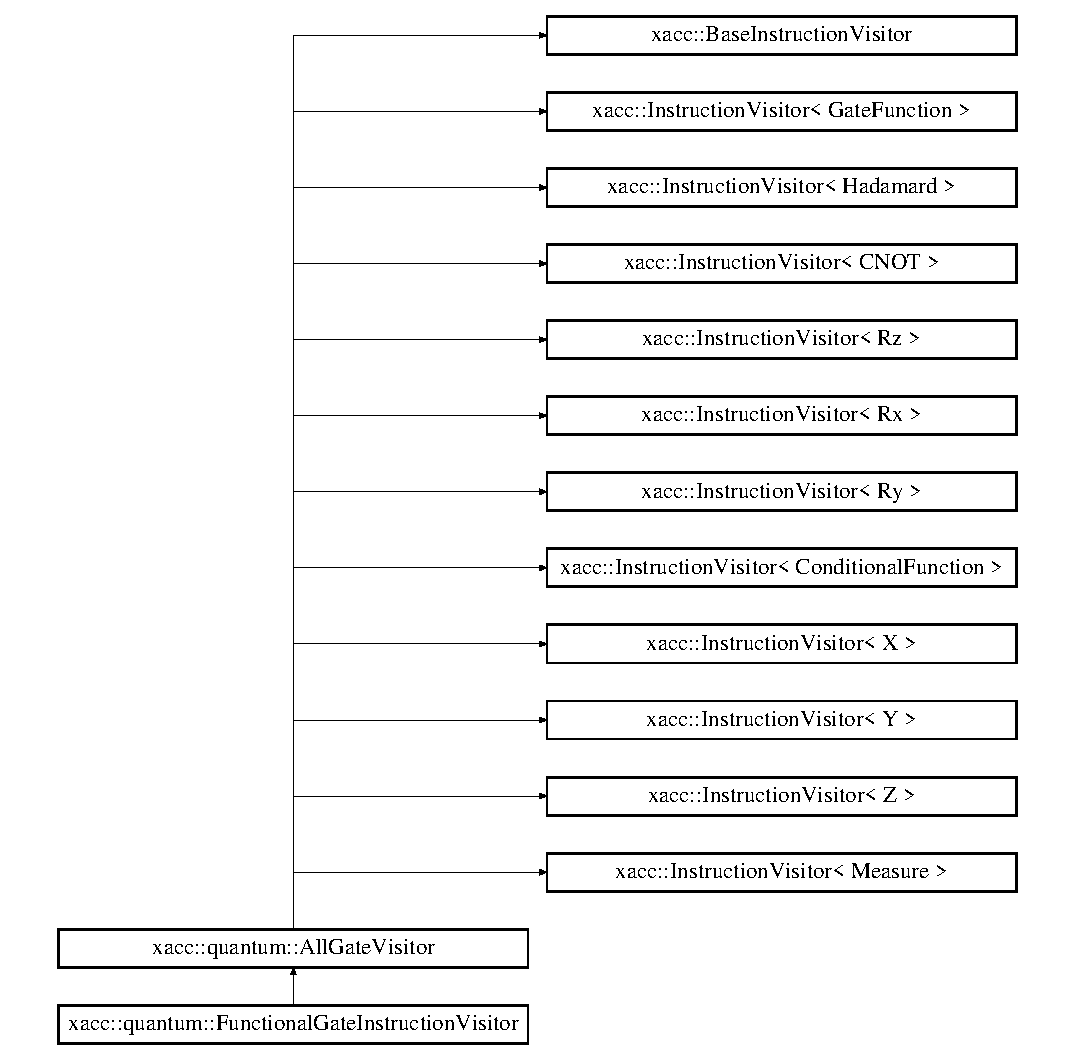
\includegraphics[height=12.000000cm]{a00031}
\end{center}
\end{figure}
\subsection*{Public Member Functions}
\begin{DoxyCompactItemize}
\item 
{\footnotesize template$<$typename HF , typename C\+NF , typename XF , typename YF , typename ZF , typename R\+XF , typename R\+YF , typename R\+ZF , typename MF , typename CF $>$ }\\{\bfseries Functional\+Gate\+Instruction\+Visitor} (HF h, C\+NF cn, XF x, YF y, ZF z, R\+XF rx, R\+YF ry, R\+ZF rz, MF m, CF c)\hypertarget{a00031_ab9e838d9bedab46a5ea54c9a0b99ef8a}{}\label{a00031_ab9e838d9bedab46a5ea54c9a0b99ef8a}

\item 
void {\bfseries visit} (\hyperlink{a00036}{Hadamard} \&h)\hypertarget{a00031_ac5245d34429dc112e7cd0e371108fcb5}{}\label{a00031_ac5245d34429dc112e7cd0e371108fcb5}

\item 
void {\bfseries visit} (\hyperlink{a00019}{C\+N\+OT} \&cn)\hypertarget{a00031_ad4eddafe8ca3906cd4aa5b98087a789a}{}\label{a00031_ad4eddafe8ca3906cd4aa5b98087a789a}

\item 
void {\bfseries visit} (\hyperlink{a00070}{X} \&x)\hypertarget{a00031_ac5d184daee7e755c9ede67b34bc2d091}{}\label{a00031_ac5d184daee7e755c9ede67b34bc2d091}

\item 
void {\bfseries visit} (\hyperlink{a00075}{Y} \&y)\hypertarget{a00031_a11dfa753a155346a45d7116a78c8f39f}{}\label{a00031_a11dfa753a155346a45d7116a78c8f39f}

\item 
void {\bfseries visit} (\hyperlink{a00076}{Z} \&z)\hypertarget{a00031_a4baf19da581fa9875739a227aba9cf60}{}\label{a00031_a4baf19da581fa9875739a227aba9cf60}

\item 
void {\bfseries visit} (\hyperlink{a00045}{Measure} \&m)\hypertarget{a00031_ad946faf8e2b6eff3e9e142907ec8e05a}{}\label{a00031_ad946faf8e2b6eff3e9e142907ec8e05a}

\item 
void {\bfseries visit} (\hyperlink{a00021}{Conditional\+Function} \&c)\hypertarget{a00031_a5cdb38902c241e7ae672a2631f1d61f3}{}\label{a00031_a5cdb38902c241e7ae672a2631f1d61f3}

\item 
void {\bfseries visit} (\hyperlink{a00061}{Rx} \&rx)\hypertarget{a00031_a6eb99e4b488773c750b7d9734ac1e885}{}\label{a00031_a6eb99e4b488773c750b7d9734ac1e885}

\item 
void {\bfseries visit} (\hyperlink{a00062}{Ry} \&ry)\hypertarget{a00031_aa22aad7b316386f5ef35672337c05ffc}{}\label{a00031_aa22aad7b316386f5ef35672337c05ffc}

\item 
void {\bfseries visit} (\hyperlink{a00063}{Rz} \&rz)\hypertarget{a00031_a8857ecf8f8f1b6143da8f31a722fe03e}{}\label{a00031_a8857ecf8f8f1b6143da8f31a722fe03e}

\item 
void {\bfseries visit} (\hyperlink{a00032}{Gate\+Function} \&f)\hypertarget{a00031_ad7d15225cf258fe59660ba828baff357}{}\label{a00031_ad7d15225cf258fe59660ba828baff357}

\end{DoxyCompactItemize}
\subsection*{Protected Attributes}
\begin{DoxyCompactItemize}
\item 
std\+::function$<$ void(\hyperlink{a00036}{Hadamard} \&)$>$ {\bfseries h\+Action}\hypertarget{a00031_a02f1401c9b0d1da801027f3bc0b5227e}{}\label{a00031_a02f1401c9b0d1da801027f3bc0b5227e}

\item 
std\+::function$<$ void(\hyperlink{a00019}{C\+N\+OT} \&)$>$ {\bfseries cnot\+Action}\hypertarget{a00031_a4d6bd8c2fd1af775ed08946942f60a0b}{}\label{a00031_a4d6bd8c2fd1af775ed08946942f60a0b}

\item 
std\+::function$<$ void(\hyperlink{a00070}{X} \&)$>$ {\bfseries x\+Action}\hypertarget{a00031_a9e0295434a2224b776609b057147a9af}{}\label{a00031_a9e0295434a2224b776609b057147a9af}

\item 
std\+::function$<$ void(\hyperlink{a00075}{Y} \&)$>$ {\bfseries y\+Action}\hypertarget{a00031_ae78f91a5cc9a7006f6bb1acee1c00501}{}\label{a00031_ae78f91a5cc9a7006f6bb1acee1c00501}

\item 
std\+::function$<$ void(\hyperlink{a00076}{Z} \&)$>$ {\bfseries z\+Action}\hypertarget{a00031_ae197f358e3d0777feb3656455e2ee672}{}\label{a00031_ae197f358e3d0777feb3656455e2ee672}

\item 
std\+::function$<$ void(\hyperlink{a00045}{Measure} \&)$>$ {\bfseries measure\+Action}\hypertarget{a00031_a239748abedd67c7b30cad12e545d1926}{}\label{a00031_a239748abedd67c7b30cad12e545d1926}

\item 
std\+::function$<$ void(\hyperlink{a00021}{Conditional\+Function} \&)$>$ {\bfseries cond\+Action}\hypertarget{a00031_a5c0595a70b1f7ae50f3e29a985e249e9}{}\label{a00031_a5c0595a70b1f7ae50f3e29a985e249e9}

\item 
std\+::function$<$ void(\hyperlink{a00061}{Rx} \&)$>$ {\bfseries rx\+Action}\hypertarget{a00031_ab79bb3eb3050d1c599061863bb2e219e}{}\label{a00031_ab79bb3eb3050d1c599061863bb2e219e}

\item 
std\+::function$<$ void(\hyperlink{a00062}{Ry} \&)$>$ {\bfseries ry\+Action}\hypertarget{a00031_a229b7d9aae52638c6eff04bd16bb9973}{}\label{a00031_a229b7d9aae52638c6eff04bd16bb9973}

\item 
std\+::function$<$ void(\hyperlink{a00063}{Rz} \&)$>$ {\bfseries rz\+Action}\hypertarget{a00031_a586ab5721150c67ad3ced46e2a236b44}{}\label{a00031_a586ab5721150c67ad3ced46e2a236b44}

\end{DoxyCompactItemize}


The documentation for this class was generated from the following file\+:\begin{DoxyCompactItemize}
\item 
Functional\+Gate\+Instruction\+Visitor.\+hpp\end{DoxyCompactItemize}

\hypertarget{a00032}{}\section{Accelerator\+Buffer Class Reference}
\label{a00032}\index{Accelerator\+Buffer@{Accelerator\+Buffer}}


{\ttfamily \#include $<$Accelerator\+Buffer.\+hpp$>$}

Inheritance diagram for Accelerator\+Buffer\+:\begin{figure}[H]
\begin{center}
\leavevmode
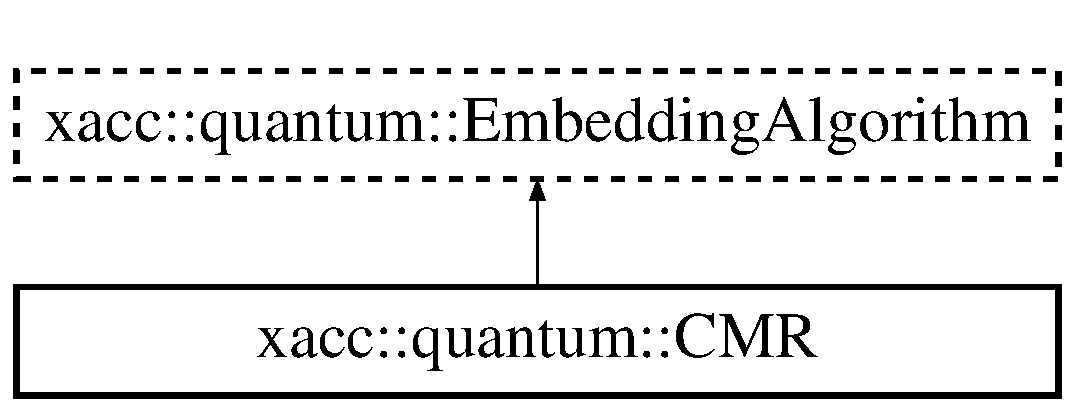
\includegraphics[height=2.000000cm]{a00032}
\end{center}
\end{figure}
\subsection*{Public Member Functions}
\begin{DoxyCompactItemize}
\item 
{\bfseries Accelerator\+Buffer} (const std\+::string \&str)\hypertarget{a00032_a5115079c3f3f8d32e713f78a91c93a7a}{}\label{a00032_a5115079c3f3f8d32e713f78a91c93a7a}

\item 
{\bfseries Accelerator\+Buffer} (const std\+::string \&str, const int N)\hypertarget{a00032_a6947082735241791c5170d677042da4a}{}\label{a00032_a6947082735241791c5170d677042da4a}

\item 
{\footnotesize template$<$typename... Indices$>$ }\\{\bfseries Accelerator\+Buffer} (const std\+::string \&str, int first\+Index, Indices...\+indices)\hypertarget{a00032_afe8b2a7e0b7b7992f45fe7021d106b66}{}\label{a00032_afe8b2a7e0b7b7992f45fe7021d106b66}

\item 
int {\bfseries size} ()\hypertarget{a00032_a249eae9f3b83072e5b101ba23f900e81}{}\label{a00032_a249eae9f3b83072e5b101ba23f900e81}

\item 
std\+::string {\bfseries name} ()\hypertarget{a00032_a3373218e4d430d061ba75135bf14ede3}{}\label{a00032_a3373218e4d430d061ba75135bf14ede3}

\item 
void {\bfseries reset\+Buffer} ()\hypertarget{a00032_aa5080c9a975871858b39d3394e867e77}{}\label{a00032_aa5080c9a975871858b39d3394e867e77}

\item 
void {\bfseries update\+Bit} (const int idx, int zero\+Or\+One)\hypertarget{a00032_a689855524e630049db6120a1493a3c45}{}\label{a00032_a689855524e630049db6120a1493a3c45}

\item 
Accelerator\+Bit\+State {\bfseries get\+Accelerator\+Bit\+State} (const int idx)\hypertarget{a00032_a29ece4f7b671308b89c06f3ac8e74b9e}{}\label{a00032_a29ece4f7b671308b89c06f3ac8e74b9e}

\item 
virtual void {\bfseries print} ()\hypertarget{a00032_a3776733a3196bca276988d4cc50a135a}{}\label{a00032_a3776733a3196bca276988d4cc50a135a}

\item 
virtual void {\bfseries print} (std\+::ostream \&stream)\hypertarget{a00032_a6f2cf905960a528fc829904a3c176c6e}{}\label{a00032_a6f2cf905960a528fc829904a3c176c6e}

\end{DoxyCompactItemize}
\subsection*{Protected Attributes}
\begin{DoxyCompactItemize}
\item 
std\+::string {\bfseries buffer\+Id}\hypertarget{a00032_adca17dc5025c067a927aefd6a5cbe51b}{}\label{a00032_adca17dc5025c067a927aefd6a5cbe51b}

\item 
std\+::vector$<$ \hyperlink{a00031}{Accelerator\+Bit} $>$ {\bfseries bits}\hypertarget{a00032_a36b3300cbada4e54e9e68d1c7c135c9b}{}\label{a00032_a36b3300cbada4e54e9e68d1c7c135c9b}

\end{DoxyCompactItemize}


\subsection{Detailed Description}
\begin{DoxyAuthor}{Author}
Alex Mc\+Caskey 
\end{DoxyAuthor}


The documentation for this class was generated from the following file\+:\begin{DoxyCompactItemize}
\item 
Accelerator\+Buffer.\+hpp\end{DoxyCompactItemize}

\hypertarget{a00033}{}\section{xacc\+:\+:quantum\+:\+:C\+N\+OT Class Reference}
\label{a00033}\index{xacc\+::quantum\+::\+C\+N\+OT@{xacc\+::quantum\+::\+C\+N\+OT}}
Inheritance diagram for xacc\+:\+:quantum\+:\+:C\+N\+OT\+:\begin{figure}[H]
\begin{center}
\leavevmode
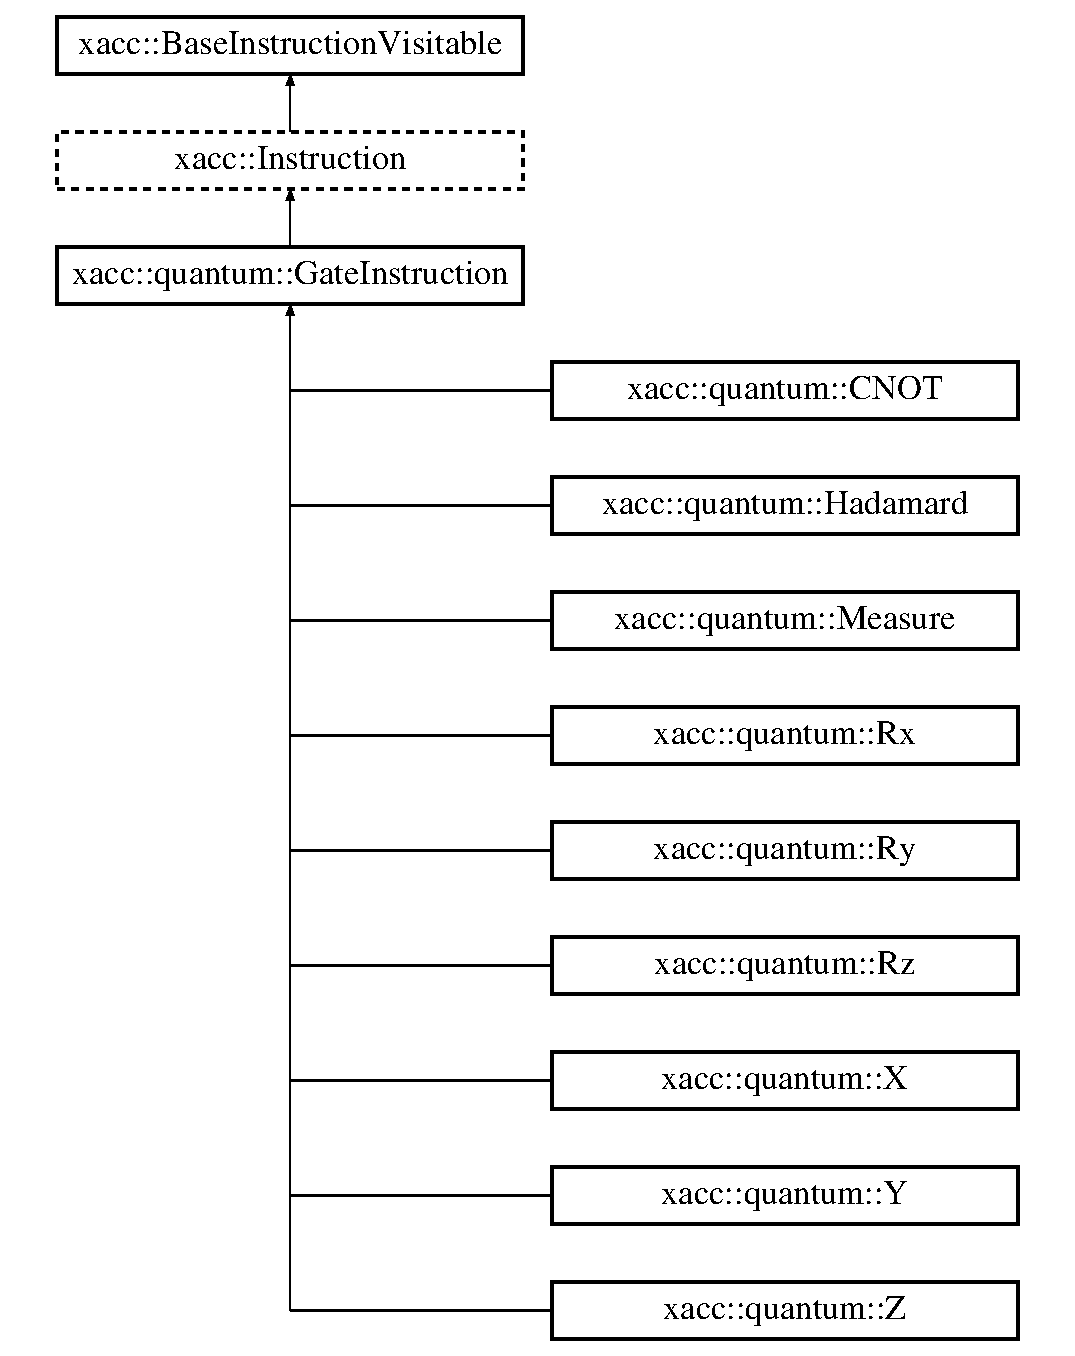
\includegraphics[height=4.000000cm]{a00033}
\end{center}
\end{figure}
\subsection*{Public Member Functions}
\begin{DoxyCompactItemize}
\item 
{\bfseries C\+N\+OT} (std\+::vector$<$ int $>$ \hyperlink{a00062_a2a56be6c2519ea65df4d06f4abae1393}{qbits})\hypertarget{a00033_ad3d460779a27affa317dd4f3a88268b3}{}\label{a00033_ad3d460779a27affa317dd4f3a88268b3}

\item 
{\bfseries C\+N\+OT} (int srcqbit, int tgtqbit)\hypertarget{a00033_a15efcb44477dde4b6151fe1776a73ddc}{}\label{a00033_a15efcb44477dde4b6151fe1776a73ddc}

\end{DoxyCompactItemize}
\subsection*{Additional Inherited Members}


The documentation for this class was generated from the following files\+:\begin{DoxyCompactItemize}
\item 
C\+N\+O\+T.\+hpp\item 
C\+N\+O\+T.\+cpp\end{DoxyCompactItemize}

\hypertarget{a00034}{}\section{xacc\+:\+:quantum\+:\+:D\+W\+Q\+M\+I\+Compiler Class Reference}
\label{a00034}\index{xacc\+::quantum\+::\+D\+W\+Q\+M\+I\+Compiler@{xacc\+::quantum\+::\+D\+W\+Q\+M\+I\+Compiler}}


{\ttfamily \#include $<$D\+W\+Q\+M\+I\+Compiler.\+hpp$>$}

Inheritance diagram for xacc\+:\+:quantum\+:\+:D\+W\+Q\+M\+I\+Compiler\+:\begin{figure}[H]
\begin{center}
\leavevmode
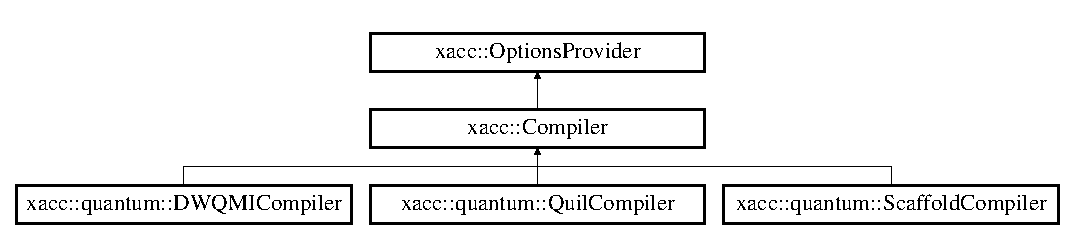
\includegraphics[height=3.000000cm]{a00034}
\end{center}
\end{figure}
\subsection*{Public Member Functions}
\begin{DoxyCompactItemize}
\item 
\hyperlink{a00034_a1f285f3eaec09363d9439676dbdfbd6a}{D\+W\+Q\+M\+I\+Compiler} ()
\item 
virtual std\+::shared\+\_\+ptr$<$ \hyperlink{a00050}{xacc\+::\+IR} $>$ \hyperlink{a00034_a0df05642f1a6fd44ce7f1c0396d50c9c}{compile} (const std\+::string \&src, std\+::shared\+\_\+ptr$<$ \hyperlink{a00011}{Accelerator} $>$ acc)
\item 
virtual std\+::shared\+\_\+ptr$<$ \hyperlink{a00050}{xacc\+::\+IR} $>$ \hyperlink{a00034_aa22591343b5509bf2c3a5820130ba906}{compile} (const std\+::string \&src)
\item 
virtual const std\+::string \hyperlink{a00034_aed42de96f8e0dd94b6de183f28aee419}{get\+Name} ()
\item 
virtual std\+::shared\+\_\+ptr$<$ options\+\_\+description $>$ \hyperlink{a00034_a0851334cc33b5b1da2694150a0a1a43c}{get\+Options} ()
\item 
virtual const std\+::string \hyperlink{a00034_a56a345539665099329209b3b5f6810c9}{translate} (const std\+::string \&buffer\+Variable, std\+::shared\+\_\+ptr$<$ \hyperlink{a00038}{Function} $>$ function)
\item 
virtual \hyperlink{a00034_a86f9135f7dc1c3246970e2a7f6540b5c}{$\sim$\+D\+W\+Q\+M\+I\+Compiler} ()
\end{DoxyCompactItemize}
\subsection*{Static Public Member Functions}
\begin{DoxyCompactItemize}
\item 
static void \hyperlink{a00034_a421daa5286f31e2b5ab4c141a34c94cd}{register\+Compiler} ()
\end{DoxyCompactItemize}
\subsection*{Additional Inherited Members}


\subsection{Detailed Description}
The \hyperlink{a00034}{D\+W\+Q\+M\+I\+Compiler} is an X\+A\+CC \hyperlink{a00023}{Compiler} that compiles D-\/\+Wave quantum machine instructions to produce an appropriate Ising form for execution on the D-\/\+Wave Q\+PU.

This compilation leverages X\+A\+CC Embedding\+Algorithms to compute the minor graph embedding represented by the input source kernel code to output the embedded Ising graph for D-\/\+Wave execution. 

\subsection{Constructor \& Destructor Documentation}
\index{xacc\+::quantum\+::\+D\+W\+Q\+M\+I\+Compiler@{xacc\+::quantum\+::\+D\+W\+Q\+M\+I\+Compiler}!D\+W\+Q\+M\+I\+Compiler@{D\+W\+Q\+M\+I\+Compiler}}
\index{D\+W\+Q\+M\+I\+Compiler@{D\+W\+Q\+M\+I\+Compiler}!xacc\+::quantum\+::\+D\+W\+Q\+M\+I\+Compiler@{xacc\+::quantum\+::\+D\+W\+Q\+M\+I\+Compiler}}
\subsubsection[{\texorpdfstring{D\+W\+Q\+M\+I\+Compiler()}{DWQMICompiler()}}]{\setlength{\rightskip}{0pt plus 5cm}xacc\+::quantum\+::\+D\+W\+Q\+M\+I\+Compiler\+::\+D\+W\+Q\+M\+I\+Compiler (
\begin{DoxyParamCaption}
{}
\end{DoxyParamCaption}
)\hspace{0.3cm}{\ttfamily [inline]}}\hypertarget{a00034_a1f285f3eaec09363d9439676dbdfbd6a}{}\label{a00034_a1f285f3eaec09363d9439676dbdfbd6a}
The \hyperlink{a00023}{Compiler}. \index{xacc\+::quantum\+::\+D\+W\+Q\+M\+I\+Compiler@{xacc\+::quantum\+::\+D\+W\+Q\+M\+I\+Compiler}!````~D\+W\+Q\+M\+I\+Compiler@{$\sim$\+D\+W\+Q\+M\+I\+Compiler}}
\index{````~D\+W\+Q\+M\+I\+Compiler@{$\sim$\+D\+W\+Q\+M\+I\+Compiler}!xacc\+::quantum\+::\+D\+W\+Q\+M\+I\+Compiler@{xacc\+::quantum\+::\+D\+W\+Q\+M\+I\+Compiler}}
\subsubsection[{\texorpdfstring{$\sim$\+D\+W\+Q\+M\+I\+Compiler()}{~DWQMICompiler()}}]{\setlength{\rightskip}{0pt plus 5cm}virtual xacc\+::quantum\+::\+D\+W\+Q\+M\+I\+Compiler\+::$\sim$\+D\+W\+Q\+M\+I\+Compiler (
\begin{DoxyParamCaption}
{}
\end{DoxyParamCaption}
)\hspace{0.3cm}{\ttfamily [inline]}, {\ttfamily [virtual]}}\hypertarget{a00034_a86f9135f7dc1c3246970e2a7f6540b5c}{}\label{a00034_a86f9135f7dc1c3246970e2a7f6540b5c}
The destructor 

\subsection{Member Function Documentation}
\index{xacc\+::quantum\+::\+D\+W\+Q\+M\+I\+Compiler@{xacc\+::quantum\+::\+D\+W\+Q\+M\+I\+Compiler}!compile@{compile}}
\index{compile@{compile}!xacc\+::quantum\+::\+D\+W\+Q\+M\+I\+Compiler@{xacc\+::quantum\+::\+D\+W\+Q\+M\+I\+Compiler}}
\subsubsection[{\texorpdfstring{compile(const std\+::string \&src, std\+::shared\+\_\+ptr$<$ Accelerator $>$ acc)}{compile(const std::string \&src, std::shared\_ptr< Accelerator > acc)}}]{\setlength{\rightskip}{0pt plus 5cm}std\+::shared\+\_\+ptr$<$ {\bf IR} $>$ xacc\+::quantum\+::\+D\+W\+Q\+M\+I\+Compiler\+::compile (
\begin{DoxyParamCaption}
\item[{const std\+::string \&}]{src, }
\item[{std\+::shared\+\_\+ptr$<$ {\bf Accelerator} $>$}]{acc}
\end{DoxyParamCaption}
)\hspace{0.3cm}{\ttfamily [virtual]}}\hypertarget{a00034_a0df05642f1a6fd44ce7f1c0396d50c9c}{}\label{a00034_a0df05642f1a6fd44ce7f1c0396d50c9c}
Compile the given kernel code for the given D-\/\+Wave \hyperlink{a00011}{Accelerator}.


\begin{DoxyParams}{Parameters}
{\em src} & The Q\+MI source code \\
\hline
{\em acc} & Reference to the D-\/\+Wave \hyperlink{a00011}{Accelerator} \\
\hline
\end{DoxyParams}
\begin{DoxyReturn}{Returns}

\end{DoxyReturn}


Implements \hyperlink{a00023_a546a40c95bb93af6a0c0ac48dbeaffc8}{xacc\+::\+Compiler}.

\index{xacc\+::quantum\+::\+D\+W\+Q\+M\+I\+Compiler@{xacc\+::quantum\+::\+D\+W\+Q\+M\+I\+Compiler}!compile@{compile}}
\index{compile@{compile}!xacc\+::quantum\+::\+D\+W\+Q\+M\+I\+Compiler@{xacc\+::quantum\+::\+D\+W\+Q\+M\+I\+Compiler}}
\subsubsection[{\texorpdfstring{compile(const std\+::string \&src)}{compile(const std::string \&src)}}]{\setlength{\rightskip}{0pt plus 5cm}std\+::shared\+\_\+ptr$<$ {\bf IR} $>$ xacc\+::quantum\+::\+D\+W\+Q\+M\+I\+Compiler\+::compile (
\begin{DoxyParamCaption}
\item[{const std\+::string \&}]{src}
\end{DoxyParamCaption}
)\hspace{0.3cm}{\ttfamily [virtual]}}\hypertarget{a00034_aa22591343b5509bf2c3a5820130ba906}{}\label{a00034_aa22591343b5509bf2c3a5820130ba906}
This method is not implemented -\/ we must always have D-\/\+Wave \hyperlink{a00011}{Accelerator} connectivity information for compilation.

\begin{DoxyReturn}{Returns}

\end{DoxyReturn}


Implements \hyperlink{a00023_a9092f5f779b570c91569b59621280c04}{xacc\+::\+Compiler}.

\index{xacc\+::quantum\+::\+D\+W\+Q\+M\+I\+Compiler@{xacc\+::quantum\+::\+D\+W\+Q\+M\+I\+Compiler}!get\+Name@{get\+Name}}
\index{get\+Name@{get\+Name}!xacc\+::quantum\+::\+D\+W\+Q\+M\+I\+Compiler@{xacc\+::quantum\+::\+D\+W\+Q\+M\+I\+Compiler}}
\subsubsection[{\texorpdfstring{get\+Name()}{getName()}}]{\setlength{\rightskip}{0pt plus 5cm}virtual const std\+::string xacc\+::quantum\+::\+D\+W\+Q\+M\+I\+Compiler\+::get\+Name (
\begin{DoxyParamCaption}
{}
\end{DoxyParamCaption}
)\hspace{0.3cm}{\ttfamily [inline]}, {\ttfamily [virtual]}}\hypertarget{a00034_aed42de96f8e0dd94b6de183f28aee419}{}\label{a00034_aed42de96f8e0dd94b6de183f28aee419}
Return the name of this \hyperlink{a00023}{Compiler} \begin{DoxyReturn}{Returns}
name \hyperlink{a00023}{Compiler} name 
\end{DoxyReturn}


Implements \hyperlink{a00023_a87fca9100e6462122f5b687c3a0fb3fb}{xacc\+::\+Compiler}.

\index{xacc\+::quantum\+::\+D\+W\+Q\+M\+I\+Compiler@{xacc\+::quantum\+::\+D\+W\+Q\+M\+I\+Compiler}!get\+Options@{get\+Options}}
\index{get\+Options@{get\+Options}!xacc\+::quantum\+::\+D\+W\+Q\+M\+I\+Compiler@{xacc\+::quantum\+::\+D\+W\+Q\+M\+I\+Compiler}}
\subsubsection[{\texorpdfstring{get\+Options()}{getOptions()}}]{\setlength{\rightskip}{0pt plus 5cm}virtual std\+::shared\+\_\+ptr$<$options\+\_\+description$>$ xacc\+::quantum\+::\+D\+W\+Q\+M\+I\+Compiler\+::get\+Options (
\begin{DoxyParamCaption}
{}
\end{DoxyParamCaption}
)\hspace{0.3cm}{\ttfamily [inline]}, {\ttfamily [virtual]}}\hypertarget{a00034_a0851334cc33b5b1da2694150a0a1a43c}{}\label{a00034_a0851334cc33b5b1da2694150a0a1a43c}
Return the command line options for this compiler

\begin{DoxyReturn}{Returns}
options Description of command line options. 
\end{DoxyReturn}


Reimplemented from \hyperlink{a00023_a9f5a8965c9c2dd895016d18264ebbe92}{xacc\+::\+Compiler}.

\index{xacc\+::quantum\+::\+D\+W\+Q\+M\+I\+Compiler@{xacc\+::quantum\+::\+D\+W\+Q\+M\+I\+Compiler}!register\+Compiler@{register\+Compiler}}
\index{register\+Compiler@{register\+Compiler}!xacc\+::quantum\+::\+D\+W\+Q\+M\+I\+Compiler@{xacc\+::quantum\+::\+D\+W\+Q\+M\+I\+Compiler}}
\subsubsection[{\texorpdfstring{register\+Compiler()}{registerCompiler()}}]{\setlength{\rightskip}{0pt plus 5cm}static void xacc\+::quantum\+::\+D\+W\+Q\+M\+I\+Compiler\+::register\+Compiler (
\begin{DoxyParamCaption}
{}
\end{DoxyParamCaption}
)\hspace{0.3cm}{\ttfamily [inline]}, {\ttfamily [static]}}\hypertarget{a00034_a421daa5286f31e2b5ab4c141a34c94cd}{}\label{a00034_a421daa5286f31e2b5ab4c141a34c94cd}
Register this \hyperlink{a00023}{Compiler} with the framework. \index{xacc\+::quantum\+::\+D\+W\+Q\+M\+I\+Compiler@{xacc\+::quantum\+::\+D\+W\+Q\+M\+I\+Compiler}!translate@{translate}}
\index{translate@{translate}!xacc\+::quantum\+::\+D\+W\+Q\+M\+I\+Compiler@{xacc\+::quantum\+::\+D\+W\+Q\+M\+I\+Compiler}}
\subsubsection[{\texorpdfstring{translate(const std\+::string \&buffer\+Variable, std\+::shared\+\_\+ptr$<$ Function $>$ function)}{translate(const std::string \&bufferVariable, std::shared\_ptr< Function > function)}}]{\setlength{\rightskip}{0pt plus 5cm}virtual const std\+::string xacc\+::quantum\+::\+D\+W\+Q\+M\+I\+Compiler\+::translate (
\begin{DoxyParamCaption}
\item[{const std\+::string \&}]{buffer\+Variable, }
\item[{std\+::shared\+\_\+ptr$<$ {\bf Function} $>$}]{function}
\end{DoxyParamCaption}
)\hspace{0.3cm}{\ttfamily [inline]}, {\ttfamily [virtual]}}\hypertarget{a00034_a56a345539665099329209b3b5f6810c9}{}\label{a00034_a56a345539665099329209b3b5f6810c9}
We don\textquotesingle{}t allow translations for the DW \hyperlink{a00023}{Compiler}. 
\begin{DoxyParams}{Parameters}
{\em buffer\+Variable} & \\
\hline
{\em function} & \\
\hline
\end{DoxyParams}
\begin{DoxyReturn}{Returns}

\end{DoxyReturn}


Implements \hyperlink{a00023_aeedbe58a33fed29e4d7694ae743e25e7}{xacc\+::\+Compiler}.



The documentation for this class was generated from the following files\+:\begin{DoxyCompactItemize}
\item 
D\+W\+Q\+M\+I\+Compiler.\+hpp\item 
D\+W\+Q\+M\+I\+Compiler.\+cpp\end{DoxyCompactItemize}

\hypertarget{a00035}{}\section{xacc\+:\+:quantum\+:\+:D\+W\+Solver Struct Reference}
\label{a00035}\index{xacc\+::quantum\+::\+D\+W\+Solver@{xacc\+::quantum\+::\+D\+W\+Solver}}


{\ttfamily \#include $<$D\+W\+Accelerator.\+hpp$>$}

\subsection*{Public Attributes}
\begin{DoxyCompactItemize}
\item 
std\+::string {\bfseries name}\hypertarget{a00035_a8a5b629dc83790a855d429c82266b772}{}\label{a00035_a8a5b629dc83790a855d429c82266b772}

\item 
std\+::string {\bfseries description}\hypertarget{a00035_a9bb9449a6ea09e11892f910a4bfd2e08}{}\label{a00035_a9bb9449a6ea09e11892f910a4bfd2e08}

\item 
double {\bfseries j\+Range\+Min}\hypertarget{a00035_a45fc23af53f44759afec0257d9878ba0}{}\label{a00035_a45fc23af53f44759afec0257d9878ba0}

\item 
double {\bfseries j\+Range\+Max}\hypertarget{a00035_aa881af1344ff55a4991c152f768ed9d6}{}\label{a00035_aa881af1344ff55a4991c152f768ed9d6}

\item 
double {\bfseries h\+Range\+Min}\hypertarget{a00035_abf475612dac8f64a7f88cfa976c393f0}{}\label{a00035_abf475612dac8f64a7f88cfa976c393f0}

\item 
double {\bfseries h\+Range\+Max}\hypertarget{a00035_a13dd875ceb06c7545fe20cde15ffac70}{}\label{a00035_a13dd875ceb06c7545fe20cde15ffac70}

\item 
int {\bfseries n\+Qubits}\hypertarget{a00035_a2908c913f5c5e3ade6551056aaadafbf}{}\label{a00035_a2908c913f5c5e3ade6551056aaadafbf}

\item 
std\+::vector$<$ std\+::pair$<$ int, int $>$ $>$ {\bfseries edges}\hypertarget{a00035_ae02cbfe68c982e50e80bcd2612c8c148}{}\label{a00035_ae02cbfe68c982e50e80bcd2612c8c148}

\end{DoxyCompactItemize}


\subsection{Detailed Description}
Wrapper for information related to the remote D-\/\+Wave solver. 

The documentation for this struct was generated from the following file\+:\begin{DoxyCompactItemize}
\item 
D\+W\+Accelerator.\+hpp\end{DoxyCompactItemize}

\hypertarget{a00036}{}\section{fire\+:\+:array\+\_\+size$<$ std\+:\+:array$<$ T, N $>$ $>$ Struct Template Reference}
\label{a00036}\index{fire\+::array\+\_\+size$<$ std\+::array$<$ T, N $>$ $>$@{fire\+::array\+\_\+size$<$ std\+::array$<$ T, N $>$ $>$}}
\subsection*{Static Public Attributes}
\begin{DoxyCompactItemize}
\item 
static const size\+\_\+t {\bfseries value} = N\hypertarget{a00036_ab92887f3c176f5d68d76c67b4db2f112}{}\label{a00036_ab92887f3c176f5d68d76c67b4db2f112}

\end{DoxyCompactItemize}


The documentation for this struct was generated from the following file\+:\begin{DoxyCompactItemize}
\item 
Tensor\+Utils.\+hpp\end{DoxyCompactItemize}

\hypertarget{a00037}{}\section{Generic\+Value$<$ Encoding, Allocator $>$\+:\+:Array\+Data Struct Reference}
\label{a00037}\index{Generic\+Value$<$ Encoding, Allocator $>$\+::\+Array\+Data@{Generic\+Value$<$ Encoding, Allocator $>$\+::\+Array\+Data}}
\subsection*{Public Attributes}
\begin{DoxyCompactItemize}
\item 
\hyperlink{a00677_a5ed6e6e67250fadbd041127e6386dcb5}{Size\+Type} {\bfseries size}\hypertarget{a00037_a5306856f64aea8ec53abf263ed2a35e2}{}\label{a00037_a5306856f64aea8ec53abf263ed2a35e2}

\item 
\hyperlink{a00677_a5ed6e6e67250fadbd041127e6386dcb5}{Size\+Type} {\bfseries capacity}\hypertarget{a00037_a0c6fe03c00e13d14b95abd31048aa1f5}{}\label{a00037_a0c6fe03c00e13d14b95abd31048aa1f5}

\item 
\hyperlink{a00130}{Generic\+Value} $\ast$ {\bfseries elements}\hypertarget{a00037_a86df976cb6f65924aca20eb9bd35553e}{}\label{a00037_a86df976cb6f65924aca20eb9bd35553e}

\end{DoxyCompactItemize}


The documentation for this struct was generated from the following file\+:\begin{DoxyCompactItemize}
\item 
\hyperlink{a00473}{document.\+h}\end{DoxyCompactItemize}

\hypertarget{a00038}{}\section{nlohmann\+:\+:basic\+\_\+json$<$ Object\+Type, Array\+Type, String\+Type, Boolean\+Type, Number\+Integer\+Type, Number\+Unsigned\+Type, Number\+Float\+Type, Allocator\+Type $>$\+:\+:const\+\_\+iterator Class Reference}
\label{a00038}\index{nlohmann\+::basic\+\_\+json$<$ Object\+Type, Array\+Type, String\+Type, Boolean\+Type, Number\+Integer\+Type, Number\+Unsigned\+Type, Number\+Float\+Type, Allocator\+Type $>$\+::const\+\_\+iterator@{nlohmann\+::basic\+\_\+json$<$ Object\+Type, Array\+Type, String\+Type, Boolean\+Type, Number\+Integer\+Type, Number\+Unsigned\+Type, Number\+Float\+Type, Allocator\+Type $>$\+::const\+\_\+iterator}}


a const random access iterator for the \hyperlink{a00025}{basic\+\_\+json} class  




{\ttfamily \#include $<$json.\+hpp$>$}

Inheritance diagram for nlohmann\+:\+:basic\+\_\+json$<$ Object\+Type, Array\+Type, String\+Type, Boolean\+Type, Number\+Integer\+Type, Number\+Unsigned\+Type, Number\+Float\+Type, Allocator\+Type $>$\+:\+:const\+\_\+iterator\+:\begin{figure}[H]
\begin{center}
\leavevmode
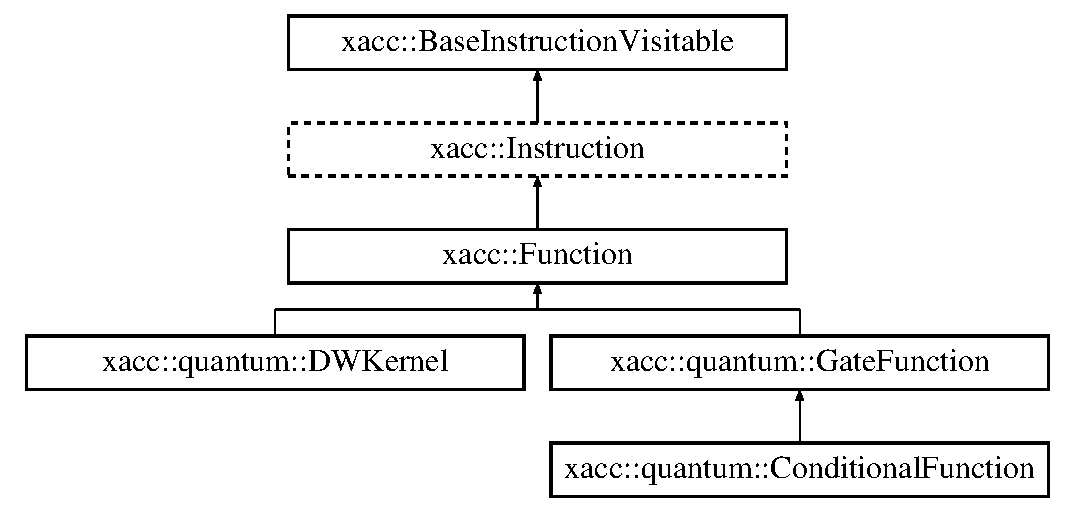
\includegraphics[height=1.705584cm]{a00038}
\end{center}
\end{figure}
\subsection*{Public Types}
\begin{DoxyCompactItemize}
\item 
using \hyperlink{a00038_a9ea0497199b1e96ce9cadd1f202ec343}{value\+\_\+type} = typename \hyperlink{a00025_ac8d45b57874b4a6e9c07f7d3b5daa1f9}{basic\+\_\+json\+::value\+\_\+type}\hypertarget{a00038_a9ea0497199b1e96ce9cadd1f202ec343}{}\label{a00038_a9ea0497199b1e96ce9cadd1f202ec343}

\begin{DoxyCompactList}\small\item\em the type of the values when the iterator is dereferenced \end{DoxyCompactList}\item 
using \hyperlink{a00038_a49d7c3e9ef3280df03052cce988b792f}{difference\+\_\+type} = typename \hyperlink{a00025_aec316934a555dd1acdd3600e5d4a4cdf}{basic\+\_\+json\+::difference\+\_\+type}\hypertarget{a00038_a49d7c3e9ef3280df03052cce988b792f}{}\label{a00038_a49d7c3e9ef3280df03052cce988b792f}

\begin{DoxyCompactList}\small\item\em a type to represent differences between iterators \end{DoxyCompactList}\item 
using \hyperlink{a00038_a1da96fc3054d547e7706d3a2f073f389}{pointer} = typename \hyperlink{a00025_a06efb200b69942eacd1ea22d0f6ccebb}{basic\+\_\+json\+::const\+\_\+pointer}\hypertarget{a00038_a1da96fc3054d547e7706d3a2f073f389}{}\label{a00038_a1da96fc3054d547e7706d3a2f073f389}

\begin{DoxyCompactList}\small\item\em defines a pointer to the type iterated over (value\+\_\+type) \end{DoxyCompactList}\item 
using \hyperlink{a00038_aefd248cac6493eed1e6ff53ba6a63eb2}{reference} = typename \hyperlink{a00025_af677a29b0e66edc9f66e5167e4667071}{basic\+\_\+json\+::const\+\_\+reference}\hypertarget{a00038_aefd248cac6493eed1e6ff53ba6a63eb2}{}\label{a00038_aefd248cac6493eed1e6ff53ba6a63eb2}

\begin{DoxyCompactList}\small\item\em defines a reference to the type iterated over (value\+\_\+type) \end{DoxyCompactList}\item 
using \hyperlink{a00038_a821560d64f50525162097f19b1392e7f}{iterator\+\_\+category} = std\+::bidirectional\+\_\+iterator\+\_\+tag\hypertarget{a00038_a821560d64f50525162097f19b1392e7f}{}\label{a00038_a821560d64f50525162097f19b1392e7f}

\begin{DoxyCompactList}\small\item\em the category of the iterator \end{DoxyCompactList}\end{DoxyCompactItemize}
\subsection*{Public Member Functions}
\begin{DoxyCompactItemize}
\item 
\hyperlink{a00038_ac6fdaff67857f82a623e5cc253917639}{const\+\_\+iterator} ()=default\hypertarget{a00038_ac6fdaff67857f82a623e5cc253917639}{}\label{a00038_ac6fdaff67857f82a623e5cc253917639}

\begin{DoxyCompactList}\small\item\em default constructor \end{DoxyCompactList}\item 
\hyperlink{a00038_a23de834b11bd895209aa65c100ab9ceb}{const\+\_\+iterator} (\hyperlink{a00038_a1da96fc3054d547e7706d3a2f073f389}{pointer} \hyperlink{a00025_ad25b2f8c21e241e2d63455537a9294ff}{object}) noexcept\hypertarget{a00038_a23de834b11bd895209aa65c100ab9ceb}{}\label{a00038_a23de834b11bd895209aa65c100ab9ceb}

\begin{DoxyCompactList}\small\item\em constructor for a given J\+S\+ON instance \end{DoxyCompactList}\item 
\hyperlink{a00038_a6b950c6bc081ac1ec1540ec05ceb2603}{const\+\_\+iterator} (const \hyperlink{a00079}{iterator} \&other) noexcept\hypertarget{a00038_a6b950c6bc081ac1ec1540ec05ceb2603}{}\label{a00038_a6b950c6bc081ac1ec1540ec05ceb2603}

\begin{DoxyCompactList}\small\item\em copy constructor given a nonconst iterator \end{DoxyCompactList}\item 
\hyperlink{a00038_a18c35a6735d3da96b4fc026421c05dd8}{const\+\_\+iterator} (const \hyperlink{a00038}{const\+\_\+iterator} \&other) noexcept\hypertarget{a00038_a18c35a6735d3da96b4fc026421c05dd8}{}\label{a00038_a18c35a6735d3da96b4fc026421c05dd8}

\begin{DoxyCompactList}\small\item\em copy constructor \end{DoxyCompactList}\item 
\hyperlink{a00038}{const\+\_\+iterator} \& \hyperlink{a00038_a5521515067b6597cb0b55a9c547a7a2b}{operator=} (\hyperlink{a00038}{const\+\_\+iterator} other) noexcept(                                       std\+::is\+\_\+nothrow\+\_\+move\+\_\+constructible$<$ \hyperlink{a00038_a1da96fc3054d547e7706d3a2f073f389}{pointer} $>$\+::\hyperlink{a00038_ac75e80d30b6169ee2a29ec93fb4d2acd}{value} and                                       std\+::is\+\_\+nothrow\+\_\+move\+\_\+assignable$<$ \hyperlink{a00038_a1da96fc3054d547e7706d3a2f073f389}{pointer} $>$\+::\hyperlink{a00038_ac75e80d30b6169ee2a29ec93fb4d2acd}{value} and                                       std\+::is\+\_\+nothrow\+\_\+move\+\_\+constructible$<$ internal\+\_\+iterator $>$\+::\hyperlink{a00038_ac75e80d30b6169ee2a29ec93fb4d2acd}{value} and                                       std\+::is\+\_\+nothrow\+\_\+move\+\_\+assignable$<$ internal\+\_\+iterator $>$\+::\hyperlink{a00038_ac75e80d30b6169ee2a29ec93fb4d2acd}{value}                       )\hypertarget{a00038_a5521515067b6597cb0b55a9c547a7a2b}{}\label{a00038_a5521515067b6597cb0b55a9c547a7a2b}

\begin{DoxyCompactList}\small\item\em copy assignment \end{DoxyCompactList}\item 
\hyperlink{a00038_aefd248cac6493eed1e6ff53ba6a63eb2}{reference} \hyperlink{a00038_ab3029a1a83cf46dc28ad443bbad0c74d}{operator$\ast$} () const \hypertarget{a00038_ab3029a1a83cf46dc28ad443bbad0c74d}{}\label{a00038_ab3029a1a83cf46dc28ad443bbad0c74d}

\begin{DoxyCompactList}\small\item\em return a reference to the value pointed to by the iterator \end{DoxyCompactList}\item 
\hyperlink{a00038_a1da96fc3054d547e7706d3a2f073f389}{pointer} \hyperlink{a00038_a8be837e4d902887676dd837abe9098d3}{operator-\/$>$} () const \hypertarget{a00038_a8be837e4d902887676dd837abe9098d3}{}\label{a00038_a8be837e4d902887676dd837abe9098d3}

\begin{DoxyCompactList}\small\item\em dereference the iterator \end{DoxyCompactList}\item 
\hyperlink{a00038}{const\+\_\+iterator} \hyperlink{a00038_a8dbaec5bf8ccba3225520356629061cb}{operator++} (int)\hypertarget{a00038_a8dbaec5bf8ccba3225520356629061cb}{}\label{a00038_a8dbaec5bf8ccba3225520356629061cb}

\begin{DoxyCompactList}\small\item\em post-\/increment (it++) \end{DoxyCompactList}\item 
\hyperlink{a00038}{const\+\_\+iterator} \& \hyperlink{a00038_a8fbb15efd97599209a7def77af8e748e}{operator++} ()\hypertarget{a00038_a8fbb15efd97599209a7def77af8e748e}{}\label{a00038_a8fbb15efd97599209a7def77af8e748e}

\begin{DoxyCompactList}\small\item\em pre-\/increment (++it) \end{DoxyCompactList}\item 
\hyperlink{a00038}{const\+\_\+iterator} \hyperlink{a00038_a6cab1c2ed7e2a014980e2a5717f43a64}{operator-\/-\/} (int)\hypertarget{a00038_a6cab1c2ed7e2a014980e2a5717f43a64}{}\label{a00038_a6cab1c2ed7e2a014980e2a5717f43a64}

\begin{DoxyCompactList}\small\item\em post-\/decrement (it--) \end{DoxyCompactList}\item 
\hyperlink{a00038}{const\+\_\+iterator} \& \hyperlink{a00038_adeb2ff3fdf3cc301b72db109934c9199}{operator-\/-\/} ()\hypertarget{a00038_adeb2ff3fdf3cc301b72db109934c9199}{}\label{a00038_adeb2ff3fdf3cc301b72db109934c9199}

\begin{DoxyCompactList}\small\item\em pre-\/decrement (--it) \end{DoxyCompactList}\item 
bool \hyperlink{a00038_ab4c0b9baaec9ebc4837158e272f6c803}{operator==} (const \hyperlink{a00038}{const\+\_\+iterator} \&other) const \hypertarget{a00038_ab4c0b9baaec9ebc4837158e272f6c803}{}\label{a00038_ab4c0b9baaec9ebc4837158e272f6c803}

\begin{DoxyCompactList}\small\item\em comparison\+: equal \end{DoxyCompactList}\item 
bool \hyperlink{a00038_a9e4c6e48e3c2f3ff357ef8215b8c8fca}{operator!=} (const \hyperlink{a00038}{const\+\_\+iterator} \&other) const \hypertarget{a00038_a9e4c6e48e3c2f3ff357ef8215b8c8fca}{}\label{a00038_a9e4c6e48e3c2f3ff357ef8215b8c8fca}

\begin{DoxyCompactList}\small\item\em comparison\+: not equal \end{DoxyCompactList}\item 
bool \hyperlink{a00038_a65f491b515e5967e9c0b40289e3c0ff3}{operator$<$} (const \hyperlink{a00038}{const\+\_\+iterator} \&other) const \hypertarget{a00038_a65f491b515e5967e9c0b40289e3c0ff3}{}\label{a00038_a65f491b515e5967e9c0b40289e3c0ff3}

\begin{DoxyCompactList}\small\item\em comparison\+: smaller \end{DoxyCompactList}\item 
bool \hyperlink{a00038_a6b682f09787eff62f03493d45aa05902}{operator$<$=} (const \hyperlink{a00038}{const\+\_\+iterator} \&other) const \hypertarget{a00038_a6b682f09787eff62f03493d45aa05902}{}\label{a00038_a6b682f09787eff62f03493d45aa05902}

\begin{DoxyCompactList}\small\item\em comparison\+: less than or equal \end{DoxyCompactList}\item 
bool \hyperlink{a00038_acb6cd0ff760933afeb7f93e5207f3646}{operator$>$} (const \hyperlink{a00038}{const\+\_\+iterator} \&other) const \hypertarget{a00038_acb6cd0ff760933afeb7f93e5207f3646}{}\label{a00038_acb6cd0ff760933afeb7f93e5207f3646}

\begin{DoxyCompactList}\small\item\em comparison\+: greater than \end{DoxyCompactList}\item 
bool \hyperlink{a00038_af6941c3711dabb2e64960dd57e00d201}{operator$>$=} (const \hyperlink{a00038}{const\+\_\+iterator} \&other) const \hypertarget{a00038_af6941c3711dabb2e64960dd57e00d201}{}\label{a00038_af6941c3711dabb2e64960dd57e00d201}

\begin{DoxyCompactList}\small\item\em comparison\+: greater than or equal \end{DoxyCompactList}\item 
\hyperlink{a00038}{const\+\_\+iterator} \& \hyperlink{a00038_a0d5820d1dda9dea3bbeb029cacf68522}{operator+=} (\hyperlink{a00038_a49d7c3e9ef3280df03052cce988b792f}{difference\+\_\+type} i)\hypertarget{a00038_a0d5820d1dda9dea3bbeb029cacf68522}{}\label{a00038_a0d5820d1dda9dea3bbeb029cacf68522}

\begin{DoxyCompactList}\small\item\em add to iterator \end{DoxyCompactList}\item 
\hyperlink{a00038}{const\+\_\+iterator} \& \hyperlink{a00038_aefac8f3e390ac917f021761f4a8f8e71}{operator-\/=} (\hyperlink{a00038_a49d7c3e9ef3280df03052cce988b792f}{difference\+\_\+type} i)\hypertarget{a00038_aefac8f3e390ac917f021761f4a8f8e71}{}\label{a00038_aefac8f3e390ac917f021761f4a8f8e71}

\begin{DoxyCompactList}\small\item\em subtract from iterator \end{DoxyCompactList}\item 
\hyperlink{a00038}{const\+\_\+iterator} \hyperlink{a00038_a7a80257f2303210b0a5d056fc0b30b40}{operator+} (\hyperlink{a00038_a49d7c3e9ef3280df03052cce988b792f}{difference\+\_\+type} i)\hypertarget{a00038_a7a80257f2303210b0a5d056fc0b30b40}{}\label{a00038_a7a80257f2303210b0a5d056fc0b30b40}

\begin{DoxyCompactList}\small\item\em add to iterator \end{DoxyCompactList}\item 
\hyperlink{a00038}{const\+\_\+iterator} \hyperlink{a00038_abc4552ba2fe39e7901a83dd6d4dec151}{operator-\/} (\hyperlink{a00038_a49d7c3e9ef3280df03052cce988b792f}{difference\+\_\+type} i)\hypertarget{a00038_abc4552ba2fe39e7901a83dd6d4dec151}{}\label{a00038_abc4552ba2fe39e7901a83dd6d4dec151}

\begin{DoxyCompactList}\small\item\em subtract from iterator \end{DoxyCompactList}\item 
\hyperlink{a00038_a49d7c3e9ef3280df03052cce988b792f}{difference\+\_\+type} \hyperlink{a00038_a5e4d98a8f95e2eccde8cd48c19efa196}{operator-\/} (const \hyperlink{a00038}{const\+\_\+iterator} \&other) const \hypertarget{a00038_a5e4d98a8f95e2eccde8cd48c19efa196}{}\label{a00038_a5e4d98a8f95e2eccde8cd48c19efa196}

\begin{DoxyCompactList}\small\item\em return difference \end{DoxyCompactList}\item 
\hyperlink{a00038_aefd248cac6493eed1e6ff53ba6a63eb2}{reference} \hyperlink{a00038_a7bd530bfbbc58ac77308c087120c21fa}{operator\mbox{[}$\,$\mbox{]}} (\hyperlink{a00038_a49d7c3e9ef3280df03052cce988b792f}{difference\+\_\+type} n) const \hypertarget{a00038_a7bd530bfbbc58ac77308c087120c21fa}{}\label{a00038_a7bd530bfbbc58ac77308c087120c21fa}

\begin{DoxyCompactList}\small\item\em access to successor \end{DoxyCompactList}\item 
object\+\_\+t\+::key\+\_\+type \hyperlink{a00038_a5d4320e24fcb7df041ff2c95d976dba0}{key} () const \hypertarget{a00038_a5d4320e24fcb7df041ff2c95d976dba0}{}\label{a00038_a5d4320e24fcb7df041ff2c95d976dba0}

\begin{DoxyCompactList}\small\item\em return the key of an object iterator \end{DoxyCompactList}\item 
\hyperlink{a00038_aefd248cac6493eed1e6ff53ba6a63eb2}{reference} \hyperlink{a00038_ac75e80d30b6169ee2a29ec93fb4d2acd}{value} () const \hypertarget{a00038_ac75e80d30b6169ee2a29ec93fb4d2acd}{}\label{a00038_ac75e80d30b6169ee2a29ec93fb4d2acd}

\begin{DoxyCompactList}\small\item\em return the value of an iterator \end{DoxyCompactList}\end{DoxyCompactItemize}
\subsection*{Friends}
\begin{DoxyCompactItemize}
\item 
class \hyperlink{a00038_ada3100cdb8700566051828f1355fa745}{basic\+\_\+json}\hypertarget{a00038_ada3100cdb8700566051828f1355fa745}{}\label{a00038_ada3100cdb8700566051828f1355fa745}

\begin{DoxyCompactList}\small\item\em allow \hyperlink{a00025}{basic\+\_\+json} to access private members \end{DoxyCompactList}\end{DoxyCompactItemize}


\subsection{Detailed Description}
\subsubsection*{template$<$template$<$ typename U, typename V, typename...\+Args $>$ class Object\+Type = std\+::map, template$<$ typename U, typename...\+Args $>$ class Array\+Type = std\+::vector, class String\+Type = std\+::string, class Boolean\+Type = bool, class Number\+Integer\+Type = int64\+\_\+t, class Number\+Unsigned\+Type = uint64\+\_\+t, class Number\+Float\+Type = double, template$<$ typename U $>$ class Allocator\+Type = std\+::allocator$>$\\*
class nlohmann\+::basic\+\_\+json$<$ Object\+Type, Array\+Type, String\+Type, Boolean\+Type, Number\+Integer\+Type, Number\+Unsigned\+Type, Number\+Float\+Type, Allocator\+Type $>$\+::const\+\_\+iterator}

a const random access iterator for the \hyperlink{a00025}{basic\+\_\+json} class 

This class implements a const iterator for the \hyperlink{a00025}{basic\+\_\+json} class. From this class, the \hyperlink{a00079}{iterator} class is derived.

The class satisfies the following concept requirements\+:
\begin{DoxyItemize}
\item \href{http://en.cppreference.com/w/cpp/concept/RandomAccessIterator}{\tt Random\+Access\+Iterator}\+: The iterator that can be moved to point (forward and backward) to any element in constant time.
\end{DoxyItemize}

\begin{DoxySince}{Since}
version 1.\+0.\+0 
\end{DoxySince}


The documentation for this class was generated from the following file\+:\begin{DoxyCompactItemize}
\item 
json.\+hpp\end{DoxyCompactItemize}

\hypertarget{a00039}{}\section{xacc\+:\+:quantum\+:\+:Functional\+Gate\+Instruction\+Visitor Class Reference}
\label{a00039}\index{xacc\+::quantum\+::\+Functional\+Gate\+Instruction\+Visitor@{xacc\+::quantum\+::\+Functional\+Gate\+Instruction\+Visitor}}
Inheritance diagram for xacc\+:\+:quantum\+:\+:Functional\+Gate\+Instruction\+Visitor\+:\begin{figure}[H]
\begin{center}
\leavevmode
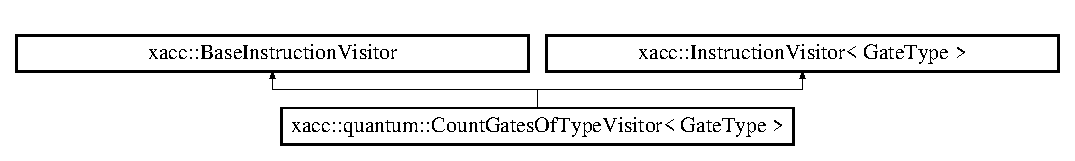
\includegraphics[height=12.000000cm]{a00039}
\end{center}
\end{figure}
\subsection*{Public Member Functions}
\begin{DoxyCompactItemize}
\item 
{\footnotesize template$<$typename HF , typename C\+NF , typename XF , typename YF , typename ZF , typename R\+XF , typename R\+YF , typename R\+ZF , typename MF , typename CF , typename C\+PF , typename S\+W\+A\+PF $>$ }\\{\bfseries Functional\+Gate\+Instruction\+Visitor} (HF h, C\+NF cn, XF x, YF y, ZF z, R\+XF rx, R\+YF ry, R\+ZF rz, MF m, CF c, C\+PF cp, S\+W\+A\+PF sw)\hypertarget{a00039_a4e3c27cd6b1acf063967b7b09a1eca09}{}\label{a00039_a4e3c27cd6b1acf063967b7b09a1eca09}

\item 
void {\bfseries visit} (\hyperlink{a00044}{Hadamard} \&h)\hypertarget{a00039_ac5245d34429dc112e7cd0e371108fcb5}{}\label{a00039_ac5245d34429dc112e7cd0e371108fcb5}

\item 
void {\bfseries visit} (\hyperlink{a00022}{C\+N\+OT} \&cn)\hypertarget{a00039_ad4eddafe8ca3906cd4aa5b98087a789a}{}\label{a00039_ad4eddafe8ca3906cd4aa5b98087a789a}

\item 
void {\bfseries visit} (\hyperlink{a00084}{X} \&x)\hypertarget{a00039_ac5d184daee7e755c9ede67b34bc2d091}{}\label{a00039_ac5d184daee7e755c9ede67b34bc2d091}

\item 
void {\bfseries visit} (\hyperlink{a00087}{Y} \&y)\hypertarget{a00039_a11dfa753a155346a45d7116a78c8f39f}{}\label{a00039_a11dfa753a155346a45d7116a78c8f39f}

\item 
void {\bfseries visit} (\hyperlink{a00088}{Z} \&z)\hypertarget{a00039_a4baf19da581fa9875739a227aba9cf60}{}\label{a00039_a4baf19da581fa9875739a227aba9cf60}

\item 
void {\bfseries visit} (\hyperlink{a00055}{Measure} \&m)\hypertarget{a00039_ad946faf8e2b6eff3e9e142907ec8e05a}{}\label{a00039_ad946faf8e2b6eff3e9e142907ec8e05a}

\item 
void {\bfseries visit} (\hyperlink{a00025}{Conditional\+Function} \&c)\hypertarget{a00039_a5cdb38902c241e7ae672a2631f1d61f3}{}\label{a00039_a5cdb38902c241e7ae672a2631f1d61f3}

\item 
void {\bfseries visit} (\hyperlink{a00073}{Rx} \&rx)\hypertarget{a00039_a6eb99e4b488773c750b7d9734ac1e885}{}\label{a00039_a6eb99e4b488773c750b7d9734ac1e885}

\item 
void {\bfseries visit} (\hyperlink{a00074}{Ry} \&ry)\hypertarget{a00039_aa22aad7b316386f5ef35672337c05ffc}{}\label{a00039_aa22aad7b316386f5ef35672337c05ffc}

\item 
void {\bfseries visit} (\hyperlink{a00027}{C\+Phase} \&cp)\hypertarget{a00039_a5475eece7afe380512a1a0215b92d302}{}\label{a00039_a5475eece7afe380512a1a0215b92d302}

\item 
void {\bfseries visit} (\hyperlink{a00075}{Rz} \&rz)\hypertarget{a00039_a8857ecf8f8f1b6143da8f31a722fe03e}{}\label{a00039_a8857ecf8f8f1b6143da8f31a722fe03e}

\item 
void {\bfseries visit} (\hyperlink{a00040}{Gate\+Function} \&f)\hypertarget{a00039_ad7d15225cf258fe59660ba828baff357}{}\label{a00039_ad7d15225cf258fe59660ba828baff357}

\item 
void {\bfseries visit} (\hyperlink{a00082}{Swap} \&s)\hypertarget{a00039_a30f46be43607813996c9cc090c1a5a16}{}\label{a00039_a30f46be43607813996c9cc090c1a5a16}

\end{DoxyCompactItemize}
\subsection*{Protected Attributes}
\begin{DoxyCompactItemize}
\item 
std\+::function$<$ void(\hyperlink{a00044}{Hadamard} \&)$>$ {\bfseries h\+Action}\hypertarget{a00039_a02f1401c9b0d1da801027f3bc0b5227e}{}\label{a00039_a02f1401c9b0d1da801027f3bc0b5227e}

\item 
std\+::function$<$ void(\hyperlink{a00022}{C\+N\+OT} \&)$>$ {\bfseries cnot\+Action}\hypertarget{a00039_a4d6bd8c2fd1af775ed08946942f60a0b}{}\label{a00039_a4d6bd8c2fd1af775ed08946942f60a0b}

\item 
std\+::function$<$ void(\hyperlink{a00084}{X} \&)$>$ {\bfseries x\+Action}\hypertarget{a00039_a9e0295434a2224b776609b057147a9af}{}\label{a00039_a9e0295434a2224b776609b057147a9af}

\item 
std\+::function$<$ void(\hyperlink{a00087}{Y} \&)$>$ {\bfseries y\+Action}\hypertarget{a00039_ae78f91a5cc9a7006f6bb1acee1c00501}{}\label{a00039_ae78f91a5cc9a7006f6bb1acee1c00501}

\item 
std\+::function$<$ void(\hyperlink{a00088}{Z} \&)$>$ {\bfseries z\+Action}\hypertarget{a00039_ae197f358e3d0777feb3656455e2ee672}{}\label{a00039_ae197f358e3d0777feb3656455e2ee672}

\item 
std\+::function$<$ void(\hyperlink{a00055}{Measure} \&)$>$ {\bfseries measure\+Action}\hypertarget{a00039_a239748abedd67c7b30cad12e545d1926}{}\label{a00039_a239748abedd67c7b30cad12e545d1926}

\item 
std\+::function$<$ void(\hyperlink{a00025}{Conditional\+Function} \&)$>$ {\bfseries cond\+Action}\hypertarget{a00039_a5c0595a70b1f7ae50f3e29a985e249e9}{}\label{a00039_a5c0595a70b1f7ae50f3e29a985e249e9}

\item 
std\+::function$<$ void(\hyperlink{a00073}{Rx} \&)$>$ {\bfseries rx\+Action}\hypertarget{a00039_ab79bb3eb3050d1c599061863bb2e219e}{}\label{a00039_ab79bb3eb3050d1c599061863bb2e219e}

\item 
std\+::function$<$ void(\hyperlink{a00074}{Ry} \&)$>$ {\bfseries ry\+Action}\hypertarget{a00039_a229b7d9aae52638c6eff04bd16bb9973}{}\label{a00039_a229b7d9aae52638c6eff04bd16bb9973}

\item 
std\+::function$<$ void(\hyperlink{a00075}{Rz} \&)$>$ {\bfseries rz\+Action}\hypertarget{a00039_a586ab5721150c67ad3ced46e2a236b44}{}\label{a00039_a586ab5721150c67ad3ced46e2a236b44}

\item 
std\+::function$<$ void(\hyperlink{a00027}{C\+Phase} \&)$>$ {\bfseries cp\+Action}\hypertarget{a00039_a5b88a0c9789e7b6d44527b2df6819ac5}{}\label{a00039_a5b88a0c9789e7b6d44527b2df6819ac5}

\item 
std\+::function$<$ void(\hyperlink{a00082}{Swap} \&)$>$ {\bfseries sw\+Action}\hypertarget{a00039_a5060cd4c2b1b259e32bda0e7ecc78e85}{}\label{a00039_a5060cd4c2b1b259e32bda0e7ecc78e85}

\end{DoxyCompactItemize}


The documentation for this class was generated from the following file\+:\begin{DoxyCompactItemize}
\item 
Functional\+Gate\+Instruction\+Visitor.\+hpp\end{DoxyCompactItemize}

\hypertarget{a00040}{}\section{Auto\+U\+TF$<$ Char\+Type $>$ Struct Template Reference}
\label{a00040}\index{Auto\+U\+T\+F$<$ Char\+Type $>$@{Auto\+U\+T\+F$<$ Char\+Type $>$}}


Dynamically select encoding according to stream\textquotesingle{}s runtime-\/specified U\+TF encoding type.  




{\ttfamily \#include $<$encodings.\+h$>$}

\subsection*{Public Types}
\begin{DoxyCompactItemize}
\item 
enum \{ {\bfseries support\+Unicode} = 1
 \}\hypertarget{a00040_aacfa2cfd9ad903c9c7110803c4037a7d}{}\label{a00040_aacfa2cfd9ad903c9c7110803c4037a7d}

\item 
typedef Char\+Type {\bfseries Ch}\hypertarget{a00040_a0609343de776df3bc31b4c980eb3cf1c}{}\label{a00040_a0609343de776df3bc31b4c980eb3cf1c}

\end{DoxyCompactItemize}
\subsection*{Static Public Member Functions}
\begin{DoxyCompactItemize}
\item 
{\footnotesize template$<$typename Output\+Stream $>$ }\\static R\+A\+P\+I\+D\+J\+S\+O\+N\+\_\+\+F\+O\+R\+C\+E\+I\+N\+L\+I\+NE void {\bfseries Encode} (Output\+Stream \&os, unsigned codepoint)\hypertarget{a00040_a414946115261f886e74dd42cb4b98781}{}\label{a00040_a414946115261f886e74dd42cb4b98781}

\item 
{\footnotesize template$<$typename Output\+Stream $>$ }\\static R\+A\+P\+I\+D\+J\+S\+O\+N\+\_\+\+F\+O\+R\+C\+E\+I\+N\+L\+I\+NE void {\bfseries Encode\+Unsafe} (Output\+Stream \&os, unsigned codepoint)\hypertarget{a00040_a05f5dcd1f153b61b763e44ed452de251}{}\label{a00040_a05f5dcd1f153b61b763e44ed452de251}

\item 
{\footnotesize template$<$typename Input\+Stream $>$ }\\static R\+A\+P\+I\+D\+J\+S\+O\+N\+\_\+\+F\+O\+R\+C\+E\+I\+N\+L\+I\+NE bool {\bfseries Decode} (Input\+Stream \&is, unsigned $\ast$codepoint)\hypertarget{a00040_aa5e3c1dc23dbb75f6442ff69500a35b0}{}\label{a00040_aa5e3c1dc23dbb75f6442ff69500a35b0}

\item 
{\footnotesize template$<$typename Input\+Stream , typename Output\+Stream $>$ }\\static R\+A\+P\+I\+D\+J\+S\+O\+N\+\_\+\+F\+O\+R\+C\+E\+I\+N\+L\+I\+NE bool {\bfseries Validate} (Input\+Stream \&is, Output\+Stream \&os)\hypertarget{a00040_a36dd6f226d6a07c12161e21c0aff20b1}{}\label{a00040_a36dd6f226d6a07c12161e21c0aff20b1}

\end{DoxyCompactItemize}


\subsection{Detailed Description}
\subsubsection*{template$<$typename Char\+Type$>$\\*
struct Auto\+U\+T\+F$<$ Char\+Type $>$}

Dynamically select encoding according to stream\textquotesingle{}s runtime-\/specified U\+TF encoding type. 

\begin{DoxyNote}{Note}
This class can be used with Auto\+U\+T\+F\+Inputt\+Stream and \hyperlink{a00042}{Auto\+U\+T\+F\+Output\+Stream}, which provides Get\+Type(). 
\end{DoxyNote}


The documentation for this struct was generated from the following file\+:\begin{DoxyCompactItemize}
\item 
encodings.\+h\end{DoxyCompactItemize}

\hypertarget{a00041}{}\section{xacc\+:\+:IR Class Reference}
\label{a00041}\index{xacc\+::\+IR@{xacc\+::\+IR}}


{\ttfamily \#include $<$I\+R.\+hpp$>$}

Inheritance diagram for xacc\+:\+:IR\+:\begin{figure}[H]
\begin{center}
\leavevmode
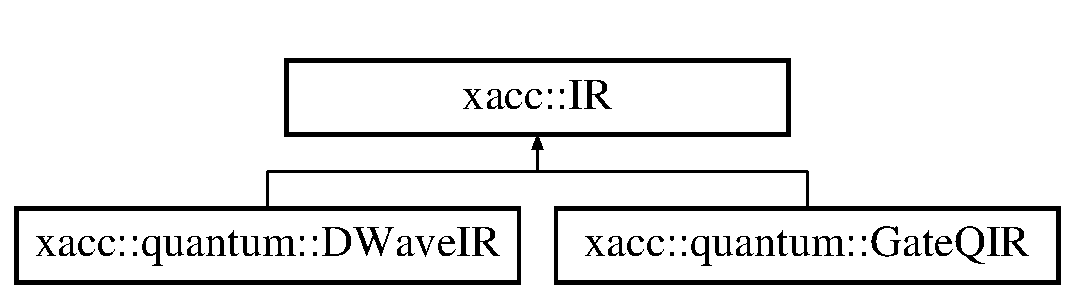
\includegraphics[height=2.000000cm]{a00041}
\end{center}
\end{figure}
\subsection*{Public Member Functions}
\begin{DoxyCompactItemize}
\item 
virtual std\+::string \hyperlink{a00041_a8356cdff1919b88eabeb84fd7450cdb6}{to\+Assembly\+String} (const std\+::string \&kernel\+Name, const std\+::string \&acc\+Buffer\+Var\+Name)=0
\item 
virtual void \hyperlink{a00041_a414b72224d88473ad6190bb88102a3ea}{persist} (std\+::ostream \&out\+Stream)=0
\item 
virtual void \hyperlink{a00041_a444c2e4dc0faac500fb70fa93997e9bc}{load} (std\+::istream \&in\+Stream)=0
\item 
virtual void \hyperlink{a00041_abbbf8e6993c518597de32cd05d49d737}{add\+Kernel} (std\+::shared\+\_\+ptr$<$ \hyperlink{a00030}{Function} $>$ kernel)=0
\item 
virtual bool \hyperlink{a00041_afc9ccf5126f3fed19c2e879133b2f6d8}{kernel\+Exists} (const std\+::string \&name)=0
\item 
virtual std\+::shared\+\_\+ptr$<$ \hyperlink{a00030}{Function} $>$ \hyperlink{a00041_a6f49b4ba4b3a15142b04873284885f0d}{get\+Kernel} (const std\+::string \&name)=0
\item 
virtual \hyperlink{a00041_a09a76d71092254acae07e19fa2f34921}{$\sim$\+IR} ()
\end{DoxyCompactItemize}


\subsection{Detailed Description}
The \hyperlink{a00041}{IR} interface is the base interface for derived accelerator-\/specific intermediate representations. At this level, an intermediate representation can be persisted to an assembly-\/like string, can be read in from file, and can be persisted to file. Since all X\+A\+CC intermediate representations operate on an \hyperlink{a00011}{Accelerator} Buffer, the \hyperlink{a00041}{IR} interface also provides a setter for such a buffer. 

\subsection{Constructor \& Destructor Documentation}
\index{xacc\+::\+IR@{xacc\+::\+IR}!````~IR@{$\sim$\+IR}}
\index{````~IR@{$\sim$\+IR}!xacc\+::\+IR@{xacc\+::\+IR}}
\subsubsection[{\texorpdfstring{$\sim$\+I\+R()}{~IR()}}]{\setlength{\rightskip}{0pt plus 5cm}virtual xacc\+::\+I\+R\+::$\sim$\+IR (
\begin{DoxyParamCaption}
{}
\end{DoxyParamCaption}
)\hspace{0.3cm}{\ttfamily [inline]}, {\ttfamily [virtual]}}\hypertarget{a00041_a09a76d71092254acae07e19fa2f34921}{}\label{a00041_a09a76d71092254acae07e19fa2f34921}
The destructor 

\subsection{Member Function Documentation}
\index{xacc\+::\+IR@{xacc\+::\+IR}!add\+Kernel@{add\+Kernel}}
\index{add\+Kernel@{add\+Kernel}!xacc\+::\+IR@{xacc\+::\+IR}}
\subsubsection[{\texorpdfstring{add\+Kernel(std\+::shared\+\_\+ptr$<$ Function $>$ kernel)=0}{addKernel(std::shared\_ptr< Function > kernel)=0}}]{\setlength{\rightskip}{0pt plus 5cm}virtual void xacc\+::\+I\+R\+::add\+Kernel (
\begin{DoxyParamCaption}
\item[{std\+::shared\+\_\+ptr$<$ {\bf Function} $>$}]{kernel}
\end{DoxyParamCaption}
)\hspace{0.3cm}{\ttfamily [pure virtual]}}\hypertarget{a00041_abbbf8e6993c518597de32cd05d49d737}{}\label{a00041_abbbf8e6993c518597de32cd05d49d737}
Add a new kernel to this \hyperlink{a00041}{IR} instance.


\begin{DoxyParams}{Parameters}
{\em kernel} & The \hyperlink{a00030}{Function} instance to add as a new kernel \\
\hline
\end{DoxyParams}


Implemented in \hyperlink{a00034_aa6ed2cf2cbcfec8105c327a4fa95346f}{xacc\+::quantum\+::\+Gate\+Q\+IR}, and \hyperlink{a00025_a7e1ddff2771233dc45f60a6b7e15ef63}{xacc\+::quantum\+::\+D\+Wave\+IR}.

\index{xacc\+::\+IR@{xacc\+::\+IR}!get\+Kernel@{get\+Kernel}}
\index{get\+Kernel@{get\+Kernel}!xacc\+::\+IR@{xacc\+::\+IR}}
\subsubsection[{\texorpdfstring{get\+Kernel(const std\+::string \&name)=0}{getKernel(const std::string \&name)=0}}]{\setlength{\rightskip}{0pt plus 5cm}virtual std\+::shared\+\_\+ptr$<${\bf Function}$>$ xacc\+::\+I\+R\+::get\+Kernel (
\begin{DoxyParamCaption}
\item[{const std\+::string \&}]{name}
\end{DoxyParamCaption}
)\hspace{0.3cm}{\ttfamily [pure virtual]}}\hypertarget{a00041_a6f49b4ba4b3a15142b04873284885f0d}{}\label{a00041_a6f49b4ba4b3a15142b04873284885f0d}
Return the kernel with the given name.


\begin{DoxyParams}{Parameters}
{\em name} & The name of the kernel to return. \\
\hline
\end{DoxyParams}
\begin{DoxyReturn}{Returns}
kernel The kernel with given name. 
\end{DoxyReturn}


Implemented in \hyperlink{a00034_a194758b6edcc3ae0c7fe8004f9bfe690}{xacc\+::quantum\+::\+Gate\+Q\+IR}, and \hyperlink{a00025_ac4295dfef98c94d7154a4fd39a6e5d1c}{xacc\+::quantum\+::\+D\+Wave\+IR}.

\index{xacc\+::\+IR@{xacc\+::\+IR}!kernel\+Exists@{kernel\+Exists}}
\index{kernel\+Exists@{kernel\+Exists}!xacc\+::\+IR@{xacc\+::\+IR}}
\subsubsection[{\texorpdfstring{kernel\+Exists(const std\+::string \&name)=0}{kernelExists(const std::string \&name)=0}}]{\setlength{\rightskip}{0pt plus 5cm}virtual bool xacc\+::\+I\+R\+::kernel\+Exists (
\begin{DoxyParamCaption}
\item[{const std\+::string \&}]{name}
\end{DoxyParamCaption}
)\hspace{0.3cm}{\ttfamily [pure virtual]}}\hypertarget{a00041_afc9ccf5126f3fed19c2e879133b2f6d8}{}\label{a00041_afc9ccf5126f3fed19c2e879133b2f6d8}
Return true if the kernel with given name exists in this \hyperlink{a00041}{IR}.


\begin{DoxyParams}{Parameters}
{\em name} & The name of the kernel to return. \\
\hline
\end{DoxyParams}
\begin{DoxyReturn}{Returns}
exists True if kernel exists. 
\end{DoxyReturn}


Implemented in \hyperlink{a00034_a692f95099caa7c024110a3f035941dca}{xacc\+::quantum\+::\+Gate\+Q\+IR}, and \hyperlink{a00025_ace9b8c6f4f29e32c8482fec4eacb637a}{xacc\+::quantum\+::\+D\+Wave\+IR}.

\index{xacc\+::\+IR@{xacc\+::\+IR}!load@{load}}
\index{load@{load}!xacc\+::\+IR@{xacc\+::\+IR}}
\subsubsection[{\texorpdfstring{load(std\+::istream \&in\+Stream)=0}{load(std::istream \&inStream)=0}}]{\setlength{\rightskip}{0pt plus 5cm}virtual void xacc\+::\+I\+R\+::load (
\begin{DoxyParamCaption}
\item[{std\+::istream \&}]{in\+Stream}
\end{DoxyParamCaption}
)\hspace{0.3cm}{\ttfamily [pure virtual]}}\hypertarget{a00041_a444c2e4dc0faac500fb70fa93997e9bc}{}\label{a00041_a444c2e4dc0faac500fb70fa93997e9bc}
Create this \hyperlink{a00041}{IR} instance from the given input stream.


\begin{DoxyParams}{Parameters}
{\em in\+Stream} & The input stream to read from. \\
\hline
\end{DoxyParams}


Implemented in \hyperlink{a00034_a07f26eeb362ac480d20da6cdc8c8fb39}{xacc\+::quantum\+::\+Gate\+Q\+IR}, and \hyperlink{a00025_a94d814172ec30c7ed32e6ab52bc2a41a}{xacc\+::quantum\+::\+D\+Wave\+IR}.

\index{xacc\+::\+IR@{xacc\+::\+IR}!persist@{persist}}
\index{persist@{persist}!xacc\+::\+IR@{xacc\+::\+IR}}
\subsubsection[{\texorpdfstring{persist(std\+::ostream \&out\+Stream)=0}{persist(std::ostream \&outStream)=0}}]{\setlength{\rightskip}{0pt plus 5cm}virtual void xacc\+::\+I\+R\+::persist (
\begin{DoxyParamCaption}
\item[{std\+::ostream \&}]{out\+Stream}
\end{DoxyParamCaption}
)\hspace{0.3cm}{\ttfamily [pure virtual]}}\hypertarget{a00041_a414b72224d88473ad6190bb88102a3ea}{}\label{a00041_a414b72224d88473ad6190bb88102a3ea}
Persist this \hyperlink{a00041}{IR} instance to the given output stream.


\begin{DoxyParams}{Parameters}
{\em out\+Stream} & The output stream to persist to. \\
\hline
\end{DoxyParams}


Implemented in \hyperlink{a00034_a40e1d07e4dfd3794ef53fca3cdbdca61}{xacc\+::quantum\+::\+Gate\+Q\+IR}, and \hyperlink{a00025_adac268c6fa2234902efeb9b3c07c0ac2}{xacc\+::quantum\+::\+D\+Wave\+IR}.

\index{xacc\+::\+IR@{xacc\+::\+IR}!to\+Assembly\+String@{to\+Assembly\+String}}
\index{to\+Assembly\+String@{to\+Assembly\+String}!xacc\+::\+IR@{xacc\+::\+IR}}
\subsubsection[{\texorpdfstring{to\+Assembly\+String(const std\+::string \&kernel\+Name, const std\+::string \&acc\+Buffer\+Var\+Name)=0}{toAssemblyString(const std::string \&kernelName, const std::string \&accBufferVarName)=0}}]{\setlength{\rightskip}{0pt plus 5cm}virtual std\+::string xacc\+::\+I\+R\+::to\+Assembly\+String (
\begin{DoxyParamCaption}
\item[{const std\+::string \&}]{kernel\+Name, }
\item[{const std\+::string \&}]{acc\+Buffer\+Var\+Name}
\end{DoxyParamCaption}
)\hspace{0.3cm}{\ttfamily [pure virtual]}}\hypertarget{a00041_a8356cdff1919b88eabeb84fd7450cdb6}{}\label{a00041_a8356cdff1919b88eabeb84fd7450cdb6}
Return a assembly-\/like string representation of this intermediate representation


\begin{DoxyParams}{Parameters}
{\em kernel\+Name} & The name of hte kernel to persist to string \\
\hline
{\em acc\+Buffer\+Var\+Name} & The name of the \hyperlink{a00013}{Accelerator\+Buffer} \\
\hline
\end{DoxyParams}
\begin{DoxyReturn}{Returns}

\end{DoxyReturn}


Implemented in \hyperlink{a00034_a7153f7e9f516d43af3d5d4f95d60bd86}{xacc\+::quantum\+::\+Gate\+Q\+IR}, and \hyperlink{a00025_ac19ad098d5bbfe769809c10e26ebebc6}{xacc\+::quantum\+::\+D\+Wave\+IR}.



The documentation for this class was generated from the following file\+:\begin{DoxyCompactItemize}
\item 
I\+R.\+hpp\end{DoxyCompactItemize}

\hypertarget{a00042}{}\section{xacc\+:\+:I\+R\+Transformation Class Reference}
\label{a00042}\index{xacc\+::\+I\+R\+Transformation@{xacc\+::\+I\+R\+Transformation}}
\subsection*{Public Member Functions}
\begin{DoxyCompactItemize}
\item 
virtual void {\bfseries transform} (\hyperlink{a00041}{IR} \&ir)=0\hypertarget{a00042_accc69cba97f39aa3e51f81fec3ccf258}{}\label{a00042_accc69cba97f39aa3e51f81fec3ccf258}

\end{DoxyCompactItemize}


The documentation for this class was generated from the following file\+:\begin{DoxyCompactItemize}
\item 
I\+R\+Transformation.\+hpp\end{DoxyCompactItemize}

\hypertarget{a00043}{}\section{xacc\+:\+:is\+\_\+valid\+\_\+vertex$<$ T, typename $>$ Struct Template Reference}
\label{a00043}\index{xacc\+::is\+\_\+valid\+\_\+vertex$<$ T, typename $>$@{xacc\+::is\+\_\+valid\+\_\+vertex$<$ T, typename $>$}}


{\ttfamily \#include $<$Graph.\+hpp$>$}

Inheritance diagram for xacc\+:\+:is\+\_\+valid\+\_\+vertex$<$ T, typename $>$\+:\begin{figure}[H]
\begin{center}
\leavevmode
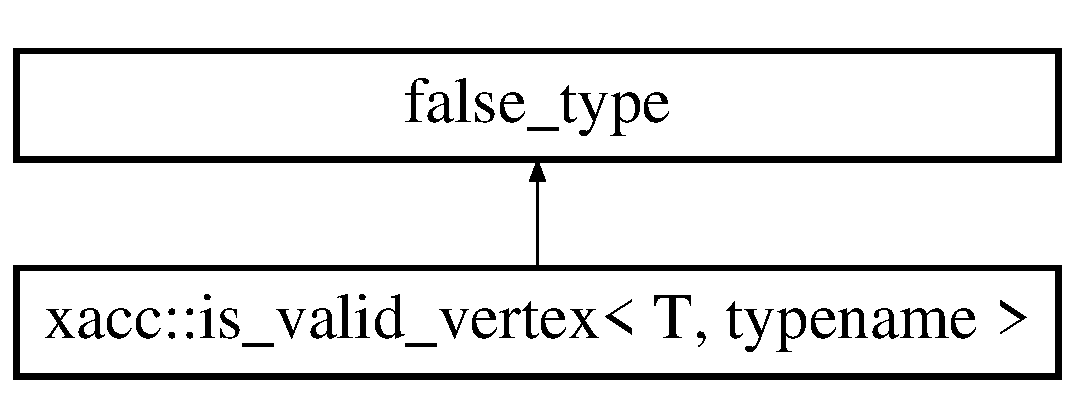
\includegraphics[height=2.000000cm]{a00043}
\end{center}
\end{figure}


\subsection{Detailed Description}
\subsubsection*{template$<$typename T, typename = void$>$\\*
struct xacc\+::is\+\_\+valid\+\_\+vertex$<$ T, typename $>$}

Utility structs to help determine if we have been given valid Vertices. 

The documentation for this struct was generated from the following file\+:\begin{DoxyCompactItemize}
\item 
Graph.\+hpp\end{DoxyCompactItemize}

\hypertarget{a00044}{}\section{xacc\+:\+:quantum\+:\+:D\+W\+IR Class Reference}
\label{a00044}\index{xacc\+::quantum\+::\+D\+W\+IR@{xacc\+::quantum\+::\+D\+W\+IR}}
Inheritance diagram for xacc\+:\+:quantum\+:\+:D\+W\+IR\+:\begin{figure}[H]
\begin{center}
\leavevmode
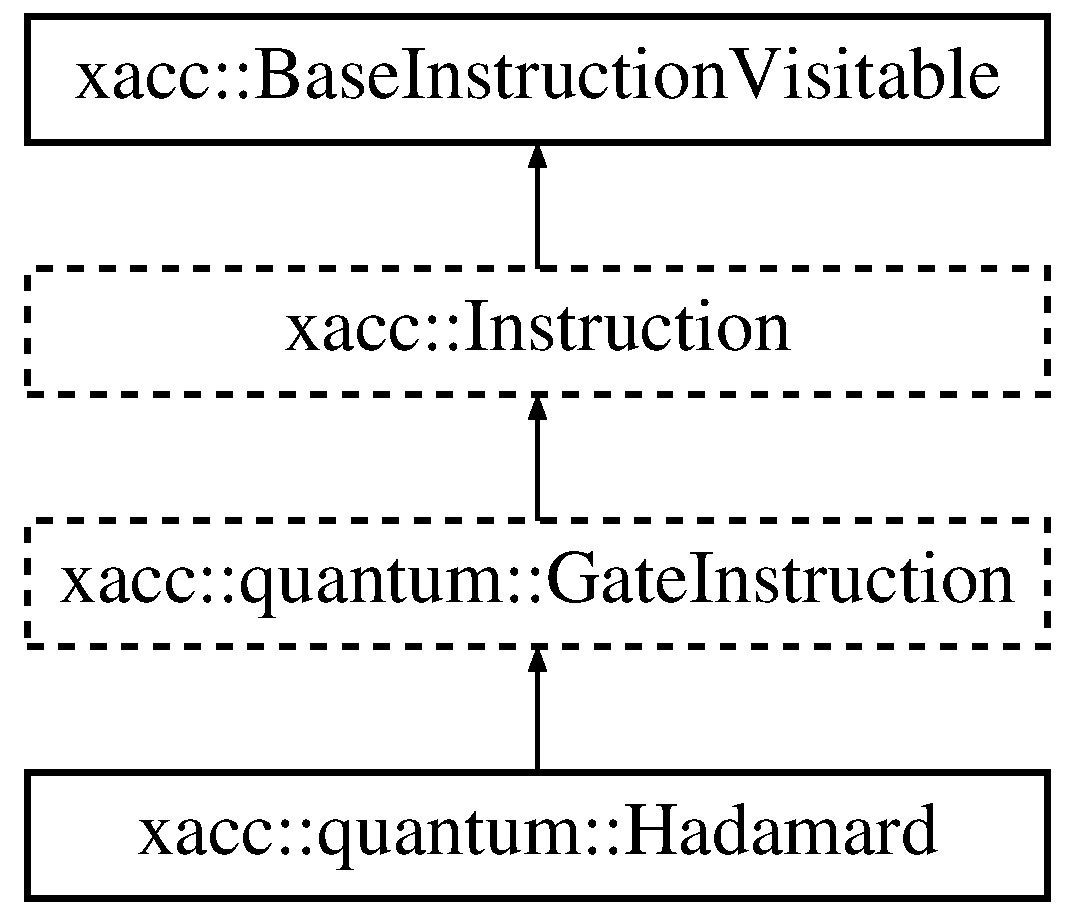
\includegraphics[height=2.000000cm]{a00044}
\end{center}
\end{figure}
\subsection*{Public Member Functions}
\begin{DoxyCompactItemize}
\item 
virtual std\+::string \hyperlink{a00044_a880cb60197577ea31115331e3a030e3e}{to\+Assembly\+String} (const std\+::string \&kernel\+Name, const std\+::string \&acc\+Buffer\+Var\+Name)
\item 
virtual void \hyperlink{a00044_abcbfd0a4cf697843391c65cbd9a82080}{persist} (std\+::ostream \&out\+Stream)
\item 
virtual void \hyperlink{a00044_a8b388d719d565bb902c979807d3d0d47}{load} (std\+::istream \&in\+Stream)
\item 
virtual void \hyperlink{a00044_af1bef18e1e9568d1313b03149aab8c1b}{add\+Kernel} (std\+::shared\+\_\+ptr$<$ \hyperlink{a00059}{Function} $>$ kernel)
\item 
virtual bool \hyperlink{a00044_ab5e8861d3bc0845bb015af6208f5f396}{kernel\+Exists} (const std\+::string \&name)
\item 
virtual std\+::shared\+\_\+ptr$<$ \hyperlink{a00059}{Function} $>$ \hyperlink{a00044_a38d8bdd24250749bc38ad31f8512fcfc}{get\+Kernel} (const std\+::string \&name)
\item 
virtual std\+::vector$<$ std\+::shared\+\_\+ptr$<$ \hyperlink{a00059}{Function} $>$ $>$ \hyperlink{a00044_a66e22c5dc95ec46045476864012ad08f}{get\+Kernels} ()
\end{DoxyCompactItemize}
\subsection*{Protected Attributes}
\begin{DoxyCompactItemize}
\item 
std\+::vector$<$ std\+::shared\+\_\+ptr$<$ \hyperlink{a00059}{Function} $>$ $>$ \hyperlink{a00044_abcb04ec3a152c3f22e5a757a9aecabf2}{kernels}
\end{DoxyCompactItemize}


\subsection{Member Function Documentation}
\index{xacc\+::quantum\+::\+D\+W\+IR@{xacc\+::quantum\+::\+D\+W\+IR}!add\+Kernel@{add\+Kernel}}
\index{add\+Kernel@{add\+Kernel}!xacc\+::quantum\+::\+D\+W\+IR@{xacc\+::quantum\+::\+D\+W\+IR}}
\subsubsection[{\texorpdfstring{add\+Kernel(std\+::shared\+\_\+ptr$<$ Function $>$ kernel)}{addKernel(std::shared\_ptr< Function > kernel)}}]{\setlength{\rightskip}{0pt plus 5cm}virtual void xacc\+::quantum\+::\+D\+W\+I\+R\+::add\+Kernel (
\begin{DoxyParamCaption}
\item[{std\+::shared\+\_\+ptr$<$ {\bf Function} $>$}]{kernel}
\end{DoxyParamCaption}
)\hspace{0.3cm}{\ttfamily [inline]}, {\ttfamily [virtual]}}\hypertarget{a00044_af1bef18e1e9568d1313b03149aab8c1b}{}\label{a00044_af1bef18e1e9568d1313b03149aab8c1b}
Add a new kernel to this \hyperlink{a00077}{IR} instance.


\begin{DoxyParams}{Parameters}
{\em kernel} & The \hyperlink{a00059}{Function} instance to add as a new kernel \\
\hline
\end{DoxyParams}


Implements \hyperlink{a00077_abbbf8e6993c518597de32cd05d49d737}{xacc\+::\+IR}.

\index{xacc\+::quantum\+::\+D\+W\+IR@{xacc\+::quantum\+::\+D\+W\+IR}!get\+Kernel@{get\+Kernel}}
\index{get\+Kernel@{get\+Kernel}!xacc\+::quantum\+::\+D\+W\+IR@{xacc\+::quantum\+::\+D\+W\+IR}}
\subsubsection[{\texorpdfstring{get\+Kernel(const std\+::string \&name)}{getKernel(const std::string \&name)}}]{\setlength{\rightskip}{0pt plus 5cm}virtual std\+::shared\+\_\+ptr$<${\bf Function}$>$ xacc\+::quantum\+::\+D\+W\+I\+R\+::get\+Kernel (
\begin{DoxyParamCaption}
\item[{const std\+::string \&}]{name}
\end{DoxyParamCaption}
)\hspace{0.3cm}{\ttfamily [inline]}, {\ttfamily [virtual]}}\hypertarget{a00044_a38d8bdd24250749bc38ad31f8512fcfc}{}\label{a00044_a38d8bdd24250749bc38ad31f8512fcfc}
Return the kernel with the given name.


\begin{DoxyParams}{Parameters}
{\em name} & The name of the kernel to return. \\
\hline
\end{DoxyParams}
\begin{DoxyReturn}{Returns}
kernel The kernel with given name. 
\end{DoxyReturn}


Implements \hyperlink{a00077_a6f49b4ba4b3a15142b04873284885f0d}{xacc\+::\+IR}.

\index{xacc\+::quantum\+::\+D\+W\+IR@{xacc\+::quantum\+::\+D\+W\+IR}!get\+Kernels@{get\+Kernels}}
\index{get\+Kernels@{get\+Kernels}!xacc\+::quantum\+::\+D\+W\+IR@{xacc\+::quantum\+::\+D\+W\+IR}}
\subsubsection[{\texorpdfstring{get\+Kernels()}{getKernels()}}]{\setlength{\rightskip}{0pt plus 5cm}virtual std\+::vector$<$std\+::shared\+\_\+ptr$<${\bf Function}$>$ $>$ xacc\+::quantum\+::\+D\+W\+I\+R\+::get\+Kernels (
\begin{DoxyParamCaption}
{}
\end{DoxyParamCaption}
)\hspace{0.3cm}{\ttfamily [inline]}, {\ttfamily [virtual]}}\hypertarget{a00044_a66e22c5dc95ec46045476864012ad08f}{}\label{a00044_a66e22c5dc95ec46045476864012ad08f}
Return all of this \hyperlink{a00077}{IR} instance\textquotesingle{}s kernels.

\begin{DoxyReturn}{Returns}
kernels The kernels this \hyperlink{a00077}{IR} contains. 
\end{DoxyReturn}


Implements \hyperlink{a00077_a88c50bfc5b279145360ddc0c3a703b9b}{xacc\+::\+IR}.

\index{xacc\+::quantum\+::\+D\+W\+IR@{xacc\+::quantum\+::\+D\+W\+IR}!kernel\+Exists@{kernel\+Exists}}
\index{kernel\+Exists@{kernel\+Exists}!xacc\+::quantum\+::\+D\+W\+IR@{xacc\+::quantum\+::\+D\+W\+IR}}
\subsubsection[{\texorpdfstring{kernel\+Exists(const std\+::string \&name)}{kernelExists(const std::string \&name)}}]{\setlength{\rightskip}{0pt plus 5cm}virtual bool xacc\+::quantum\+::\+D\+W\+I\+R\+::kernel\+Exists (
\begin{DoxyParamCaption}
\item[{const std\+::string \&}]{name}
\end{DoxyParamCaption}
)\hspace{0.3cm}{\ttfamily [inline]}, {\ttfamily [virtual]}}\hypertarget{a00044_ab5e8861d3bc0845bb015af6208f5f396}{}\label{a00044_ab5e8861d3bc0845bb015af6208f5f396}
Return true if the kernel with given name exists in this \hyperlink{a00077}{IR}.


\begin{DoxyParams}{Parameters}
{\em name} & The name of the kernel to return. \\
\hline
\end{DoxyParams}
\begin{DoxyReturn}{Returns}
exists True if kernel exists. 
\end{DoxyReturn}


Implements \hyperlink{a00077_afc9ccf5126f3fed19c2e879133b2f6d8}{xacc\+::\+IR}.

\index{xacc\+::quantum\+::\+D\+W\+IR@{xacc\+::quantum\+::\+D\+W\+IR}!load@{load}}
\index{load@{load}!xacc\+::quantum\+::\+D\+W\+IR@{xacc\+::quantum\+::\+D\+W\+IR}}
\subsubsection[{\texorpdfstring{load(std\+::istream \&in\+Stream)}{load(std::istream \&inStream)}}]{\setlength{\rightskip}{0pt plus 5cm}virtual void xacc\+::quantum\+::\+D\+W\+I\+R\+::load (
\begin{DoxyParamCaption}
\item[{std\+::istream \&}]{in\+Stream}
\end{DoxyParamCaption}
)\hspace{0.3cm}{\ttfamily [inline]}, {\ttfamily [virtual]}}\hypertarget{a00044_a8b388d719d565bb902c979807d3d0d47}{}\label{a00044_a8b388d719d565bb902c979807d3d0d47}
Create this \hyperlink{a00077}{IR} instance from the given input stream.


\begin{DoxyParams}{Parameters}
{\em in\+Stream} & \\
\hline
\end{DoxyParams}


Implements \hyperlink{a00077_a444c2e4dc0faac500fb70fa93997e9bc}{xacc\+::\+IR}.

\index{xacc\+::quantum\+::\+D\+W\+IR@{xacc\+::quantum\+::\+D\+W\+IR}!persist@{persist}}
\index{persist@{persist}!xacc\+::quantum\+::\+D\+W\+IR@{xacc\+::quantum\+::\+D\+W\+IR}}
\subsubsection[{\texorpdfstring{persist(std\+::ostream \&out\+Stream)}{persist(std::ostream \&outStream)}}]{\setlength{\rightskip}{0pt plus 5cm}virtual void xacc\+::quantum\+::\+D\+W\+I\+R\+::persist (
\begin{DoxyParamCaption}
\item[{std\+::ostream \&}]{out\+Stream}
\end{DoxyParamCaption}
)\hspace{0.3cm}{\ttfamily [inline]}, {\ttfamily [virtual]}}\hypertarget{a00044_abcbfd0a4cf697843391c65cbd9a82080}{}\label{a00044_abcbfd0a4cf697843391c65cbd9a82080}
Persist this \hyperlink{a00077}{IR} instance to the given output stream.


\begin{DoxyParams}{Parameters}
{\em out\+Stream} & \\
\hline
\end{DoxyParams}


Implements \hyperlink{a00077_a414b72224d88473ad6190bb88102a3ea}{xacc\+::\+IR}.

\index{xacc\+::quantum\+::\+D\+W\+IR@{xacc\+::quantum\+::\+D\+W\+IR}!to\+Assembly\+String@{to\+Assembly\+String}}
\index{to\+Assembly\+String@{to\+Assembly\+String}!xacc\+::quantum\+::\+D\+W\+IR@{xacc\+::quantum\+::\+D\+W\+IR}}
\subsubsection[{\texorpdfstring{to\+Assembly\+String(const std\+::string \&kernel\+Name, const std\+::string \&acc\+Buffer\+Var\+Name)}{toAssemblyString(const std::string \&kernelName, const std::string \&accBufferVarName)}}]{\setlength{\rightskip}{0pt plus 5cm}virtual std\+::string xacc\+::quantum\+::\+D\+W\+I\+R\+::to\+Assembly\+String (
\begin{DoxyParamCaption}
\item[{const std\+::string \&}]{kernel\+Name, }
\item[{const std\+::string \&}]{acc\+Buffer\+Var\+Name}
\end{DoxyParamCaption}
)\hspace{0.3cm}{\ttfamily [inline]}, {\ttfamily [virtual]}}\hypertarget{a00044_a880cb60197577ea31115331e3a030e3e}{}\label{a00044_a880cb60197577ea31115331e3a030e3e}
Return a assembly-\/like string representation of this intermediate representation \begin{DoxyReturn}{Returns}

\end{DoxyReturn}


Implements \hyperlink{a00077_a8356cdff1919b88eabeb84fd7450cdb6}{xacc\+::\+IR}.



\subsection{Member Data Documentation}
\index{xacc\+::quantum\+::\+D\+W\+IR@{xacc\+::quantum\+::\+D\+W\+IR}!kernels@{kernels}}
\index{kernels@{kernels}!xacc\+::quantum\+::\+D\+W\+IR@{xacc\+::quantum\+::\+D\+W\+IR}}
\subsubsection[{\texorpdfstring{kernels}{kernels}}]{\setlength{\rightskip}{0pt plus 5cm}std\+::vector$<$std\+::shared\+\_\+ptr$<${\bf Function}$>$ $>$ xacc\+::quantum\+::\+D\+W\+I\+R\+::kernels\hspace{0.3cm}{\ttfamily [protected]}}\hypertarget{a00044_abcb04ec3a152c3f22e5a757a9aecabf2}{}\label{a00044_abcb04ec3a152c3f22e5a757a9aecabf2}
Reference to this Q\+IR\textquotesingle{}s list of quantum functions 

The documentation for this class was generated from the following file\+:\begin{DoxyCompactItemize}
\item 
D\+W\+I\+R.\+hpp\end{DoxyCompactItemize}

\hypertarget{a00045}{}\section{xacc\+:\+:quantum\+:\+:D\+W\+Kernel Class Reference}
\label{a00045}\index{xacc\+::quantum\+::\+D\+W\+Kernel@{xacc\+::quantum\+::\+D\+W\+Kernel}}


{\ttfamily \#include $<$D\+W\+Kernel.\+hpp$>$}

Inheritance diagram for xacc\+:\+:quantum\+:\+:D\+W\+Kernel\+:\begin{figure}[H]
\begin{center}
\leavevmode
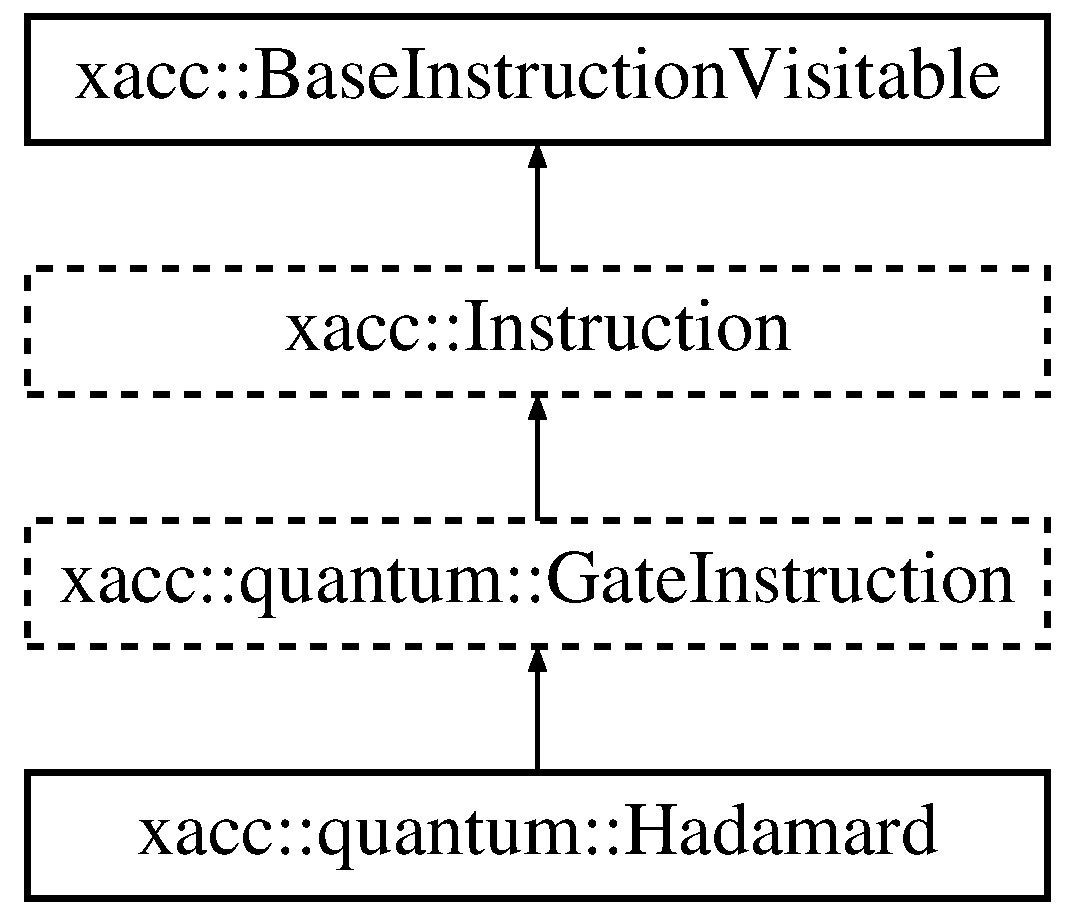
\includegraphics[height=4.000000cm]{a00045}
\end{center}
\end{figure}
\subsection*{Public Member Functions}
\begin{DoxyCompactItemize}
\item 
\hyperlink{a00045_a76a4dfadb973abbc93d1afefc6839ad8}{D\+W\+Kernel} (std\+::string kernel\+Name)
\item 
virtual const int \hyperlink{a00045_a79aecc7419a20b8779372ef36fc24806}{n\+Instructions} ()
\item 
virtual Inst\+Ptr \hyperlink{a00045_a00f23cd2e15ea6b9d00d4f3dbe1540f8}{get\+Instruction} (const int idx)
\item 
virtual std\+::list$<$ Inst\+Ptr $>$ \hyperlink{a00045_abbb8f2b1c78623c377524e45d581d018}{get\+Instructions} ()
\item 
virtual void \hyperlink{a00045_af2bcfd679e6cb89194f3f0bff8622b99}{remove\+Instruction} (const int idx)
\item 
virtual void \hyperlink{a00045_a4c3043d6971999c3a09e797fc55deb6c}{add\+Instruction} (Inst\+Ptr instruction)
\item 
virtual void \hyperlink{a00045_a75eb3560d2f81c9a5ae1cf765deb0e83}{replace\+Instruction} (const int idx, Inst\+Ptr replacing\+Inst)
\item 
virtual void \hyperlink{a00045_a1627af0141f70fc4a3cd500a13fb31b8}{insert\+Instruction} (const int idx, Inst\+Ptr new\+Inst)
\item 
virtual const std\+::string \hyperlink{a00045_a7f0c4d3c73029566561cf56a474bcbbd}{get\+Name} ()
\item 
virtual const std\+::vector$<$ int $>$ \hyperlink{a00045_adae68964db6acd8b4c2267c270a8ec58}{bits} ()
\item 
virtual const std\+::string \hyperlink{a00045_adbc3fdd080ebba20bc620b8832979f16}{to\+String} (const std\+::string \&buffer\+Var\+Name)
\item 
std\+::vector$<$ double $>$ {\bfseries get\+All\+Biases} ()\hypertarget{a00045_a9ee05b3d7689bbf837bdb7737f9745f4}{}\label{a00045_a9ee05b3d7689bbf837bdb7737f9745f4}

\item 
std\+::vector$<$ double $>$ {\bfseries get\+All\+Couplers} ()\hypertarget{a00045_a7df03ecec9c1821433daa3aa092cbd4d}{}\label{a00045_a7df03ecec9c1821433daa3aa092cbd4d}

\item 
virtual Instruction\+Parameter \hyperlink{a00045_a81711b7db284aba35d6952e4d1d15d41}{get\+Parameter} (const int idx)
\item 
virtual void \hyperlink{a00045_adf89cdd1f54e183c4cff36b338b2be8d}{set\+Parameter} (const int idx, Instruction\+Parameter \&p)
\item 
virtual std\+::vector$<$ Instruction\+Parameter $>$ \hyperlink{a00045_a829462cff34e2257da06afd8a2051a8e}{get\+Parameters} ()
\item 
virtual bool \hyperlink{a00045_a8957ea368244ed4a4ebd85f6bfecb785}{is\+Parameterized} ()
\item 
virtual const int \hyperlink{a00045_a029429948329b94c1d89f32cf5c486d4}{n\+Parameters} ()
\item 
virtual void \hyperlink{a00045_a09ffac417d4ecbbd82d7a680ad8dfcce}{evaluate\+Variable\+Parameters} (std\+::vector$<$ Instruction\+Parameter $>$ parameters)
\end{DoxyCompactItemize}
\subsection*{Protected Attributes}
\begin{DoxyCompactItemize}
\item 
std\+::list$<$ Inst\+Ptr $>$ {\bfseries instructions}\hypertarget{a00045_a38e434be6ef46a1ff43744632ae59ea8}{}\label{a00045_a38e434be6ef46a1ff43744632ae59ea8}

\item 
std\+::string {\bfseries name}\hypertarget{a00045_a0df03f85cc3b8a4cd1a7fc839d4d303c}{}\label{a00045_a0df03f85cc3b8a4cd1a7fc839d4d303c}

\end{DoxyCompactItemize}
\subsection*{Additional Inherited Members}


\subsection{Detailed Description}
The \hyperlink{a00045}{D\+W\+Kernel} is an X\+A\+CC \hyperlink{a00059}{Function} that contains \hyperlink{a00046}{D\+W\+Q\+MI} Instructions. 

\subsection{Constructor \& Destructor Documentation}
\index{xacc\+::quantum\+::\+D\+W\+Kernel@{xacc\+::quantum\+::\+D\+W\+Kernel}!D\+W\+Kernel@{D\+W\+Kernel}}
\index{D\+W\+Kernel@{D\+W\+Kernel}!xacc\+::quantum\+::\+D\+W\+Kernel@{xacc\+::quantum\+::\+D\+W\+Kernel}}
\subsubsection[{\texorpdfstring{D\+W\+Kernel(std\+::string kernel\+Name)}{DWKernel(std::string kernelName)}}]{\setlength{\rightskip}{0pt plus 5cm}xacc\+::quantum\+::\+D\+W\+Kernel\+::\+D\+W\+Kernel (
\begin{DoxyParamCaption}
\item[{std\+::string}]{kernel\+Name}
\end{DoxyParamCaption}
)\hspace{0.3cm}{\ttfamily [inline]}}\hypertarget{a00045_a76a4dfadb973abbc93d1afefc6839ad8}{}\label{a00045_a76a4dfadb973abbc93d1afefc6839ad8}
The constructor, takes the function unique id and its name.


\begin{DoxyParams}{Parameters}
{\em id} & \\
\hline
{\em name} & \\
\hline
\end{DoxyParams}


\subsection{Member Function Documentation}
\index{xacc\+::quantum\+::\+D\+W\+Kernel@{xacc\+::quantum\+::\+D\+W\+Kernel}!add\+Instruction@{add\+Instruction}}
\index{add\+Instruction@{add\+Instruction}!xacc\+::quantum\+::\+D\+W\+Kernel@{xacc\+::quantum\+::\+D\+W\+Kernel}}
\subsubsection[{\texorpdfstring{add\+Instruction(\+Inst\+Ptr instruction)}{addInstruction(InstPtr instruction)}}]{\setlength{\rightskip}{0pt plus 5cm}virtual void xacc\+::quantum\+::\+D\+W\+Kernel\+::add\+Instruction (
\begin{DoxyParamCaption}
\item[{Inst\+Ptr}]{instruction}
\end{DoxyParamCaption}
)\hspace{0.3cm}{\ttfamily [inline]}, {\ttfamily [virtual]}}\hypertarget{a00045_a4c3043d6971999c3a09e797fc55deb6c}{}\label{a00045_a4c3043d6971999c3a09e797fc55deb6c}
Add an instruction to this quantum intermediate representation.


\begin{DoxyParams}{Parameters}
{\em instruction} & \\
\hline
\end{DoxyParams}


Implements \hyperlink{a00059_aa8c9ec2d08be75c69399d4254b0216f5}{xacc\+::\+Function}.

\index{xacc\+::quantum\+::\+D\+W\+Kernel@{xacc\+::quantum\+::\+D\+W\+Kernel}!bits@{bits}}
\index{bits@{bits}!xacc\+::quantum\+::\+D\+W\+Kernel@{xacc\+::quantum\+::\+D\+W\+Kernel}}
\subsubsection[{\texorpdfstring{bits()}{bits()}}]{\setlength{\rightskip}{0pt plus 5cm}virtual const std\+::vector$<$int$>$ xacc\+::quantum\+::\+D\+W\+Kernel\+::bits (
\begin{DoxyParamCaption}
{}
\end{DoxyParamCaption}
)\hspace{0.3cm}{\ttfamily [inline]}, {\ttfamily [virtual]}}\hypertarget{a00045_adae68964db6acd8b4c2267c270a8ec58}{}\label{a00045_adae68964db6acd8b4c2267c270a8ec58}
Return the qubits this function acts on. \begin{DoxyReturn}{Returns}

\end{DoxyReturn}


Implements \hyperlink{a00072_a819f32e94c3e1c9e69a0061aaf8d86dc}{xacc\+::\+Instruction}.

\index{xacc\+::quantum\+::\+D\+W\+Kernel@{xacc\+::quantum\+::\+D\+W\+Kernel}!evaluate\+Variable\+Parameters@{evaluate\+Variable\+Parameters}}
\index{evaluate\+Variable\+Parameters@{evaluate\+Variable\+Parameters}!xacc\+::quantum\+::\+D\+W\+Kernel@{xacc\+::quantum\+::\+D\+W\+Kernel}}
\subsubsection[{\texorpdfstring{evaluate\+Variable\+Parameters(std\+::vector$<$ Instruction\+Parameter $>$ parameters)}{evaluateVariableParameters(std::vector< InstructionParameter > parameters)}}]{\setlength{\rightskip}{0pt plus 5cm}virtual void xacc\+::quantum\+::\+D\+W\+Kernel\+::evaluate\+Variable\+Parameters (
\begin{DoxyParamCaption}
\item[{std\+::vector$<$ Instruction\+Parameter $>$}]{parameters}
\end{DoxyParamCaption}
)\hspace{0.3cm}{\ttfamily [inline]}, {\ttfamily [virtual]}}\hypertarget{a00045_a09ffac417d4ecbbd82d7a680ad8dfcce}{}\label{a00045_a09ffac417d4ecbbd82d7a680ad8dfcce}
This method is used to evaluate this \hyperlink{a00059}{Function}\textquotesingle{}s parameterized Instructions that have string variable Instruction\+Parameters. These parameters are updated with the given runtime parameters.


\begin{DoxyParams}{Parameters}
{\em parameters} & The runtime parameters \\
\hline
\end{DoxyParams}


Implements \hyperlink{a00059_af6ae9453027789a2aaec30e59c9e45e3}{xacc\+::\+Function}.

\index{xacc\+::quantum\+::\+D\+W\+Kernel@{xacc\+::quantum\+::\+D\+W\+Kernel}!get\+Instruction@{get\+Instruction}}
\index{get\+Instruction@{get\+Instruction}!xacc\+::quantum\+::\+D\+W\+Kernel@{xacc\+::quantum\+::\+D\+W\+Kernel}}
\subsubsection[{\texorpdfstring{get\+Instruction(const int idx)}{getInstruction(const int idx)}}]{\setlength{\rightskip}{0pt plus 5cm}virtual Inst\+Ptr xacc\+::quantum\+::\+D\+W\+Kernel\+::get\+Instruction (
\begin{DoxyParamCaption}
\item[{const int}]{idx}
\end{DoxyParamCaption}
)\hspace{0.3cm}{\ttfamily [inline]}, {\ttfamily [virtual]}}\hypertarget{a00045_a00f23cd2e15ea6b9d00d4f3dbe1540f8}{}\label{a00045_a00f23cd2e15ea6b9d00d4f3dbe1540f8}
Return the \hyperlink{a00072}{Instruction} at the given index.


\begin{DoxyParams}{Parameters}
{\em idx} & The desired \hyperlink{a00072}{Instruction} index \\
\hline
\end{DoxyParams}
\begin{DoxyReturn}{Returns}
inst The instruction at the given index. 
\end{DoxyReturn}


Implements \hyperlink{a00059_afa549fc91b5a05f26d8139954a7e0ed5}{xacc\+::\+Function}.

\index{xacc\+::quantum\+::\+D\+W\+Kernel@{xacc\+::quantum\+::\+D\+W\+Kernel}!get\+Instructions@{get\+Instructions}}
\index{get\+Instructions@{get\+Instructions}!xacc\+::quantum\+::\+D\+W\+Kernel@{xacc\+::quantum\+::\+D\+W\+Kernel}}
\subsubsection[{\texorpdfstring{get\+Instructions()}{getInstructions()}}]{\setlength{\rightskip}{0pt plus 5cm}virtual std\+::list$<$Inst\+Ptr$>$ xacc\+::quantum\+::\+D\+W\+Kernel\+::get\+Instructions (
\begin{DoxyParamCaption}
{}
\end{DoxyParamCaption}
)\hspace{0.3cm}{\ttfamily [inline]}, {\ttfamily [virtual]}}\hypertarget{a00045_abbb8f2b1c78623c377524e45d581d018}{}\label{a00045_abbb8f2b1c78623c377524e45d581d018}
Return all Instructions in this \hyperlink{a00059}{Function}

\begin{DoxyReturn}{Returns}
insts The list of this \hyperlink{a00059}{Function}\textquotesingle{}s Instructions 
\end{DoxyReturn}


Implements \hyperlink{a00059_aaf80bd3d49113a92b520785572663032}{xacc\+::\+Function}.

\index{xacc\+::quantum\+::\+D\+W\+Kernel@{xacc\+::quantum\+::\+D\+W\+Kernel}!get\+Name@{get\+Name}}
\index{get\+Name@{get\+Name}!xacc\+::quantum\+::\+D\+W\+Kernel@{xacc\+::quantum\+::\+D\+W\+Kernel}}
\subsubsection[{\texorpdfstring{get\+Name()}{getName()}}]{\setlength{\rightskip}{0pt plus 5cm}virtual const std\+::string xacc\+::quantum\+::\+D\+W\+Kernel\+::get\+Name (
\begin{DoxyParamCaption}
{}
\end{DoxyParamCaption}
)\hspace{0.3cm}{\ttfamily [inline]}, {\ttfamily [virtual]}}\hypertarget{a00045_a7f0c4d3c73029566561cf56a474bcbbd}{}\label{a00045_a7f0c4d3c73029566561cf56a474bcbbd}
Return the name of this function \begin{DoxyReturn}{Returns}

\end{DoxyReturn}


Implements \hyperlink{a00072_ac7ff23f693e2276edbf3fdac5452792c}{xacc\+::\+Instruction}.

\index{xacc\+::quantum\+::\+D\+W\+Kernel@{xacc\+::quantum\+::\+D\+W\+Kernel}!get\+Parameter@{get\+Parameter}}
\index{get\+Parameter@{get\+Parameter}!xacc\+::quantum\+::\+D\+W\+Kernel@{xacc\+::quantum\+::\+D\+W\+Kernel}}
\subsubsection[{\texorpdfstring{get\+Parameter(const int idx)}{getParameter(const int idx)}}]{\setlength{\rightskip}{0pt plus 5cm}virtual Instruction\+Parameter xacc\+::quantum\+::\+D\+W\+Kernel\+::get\+Parameter (
\begin{DoxyParamCaption}
\item[{const int}]{idx}
\end{DoxyParamCaption}
)\hspace{0.3cm}{\ttfamily [inline]}, {\ttfamily [virtual]}}\hypertarget{a00045_a81711b7db284aba35d6952e4d1d15d41}{}\label{a00045_a81711b7db284aba35d6952e4d1d15d41}
Return this \hyperlink{a00072}{Instruction}\textquotesingle{}s parameter at the given index.


\begin{DoxyParams}{Parameters}
{\em idx} & The index of the parameter. \\
\hline
\end{DoxyParams}
\begin{DoxyReturn}{Returns}
param The Instruction\+Parameter at the given index. 
\end{DoxyReturn}


Implements \hyperlink{a00072_aa0d9de97a4833a042379647f83c33ab6}{xacc\+::\+Instruction}.

\index{xacc\+::quantum\+::\+D\+W\+Kernel@{xacc\+::quantum\+::\+D\+W\+Kernel}!get\+Parameters@{get\+Parameters}}
\index{get\+Parameters@{get\+Parameters}!xacc\+::quantum\+::\+D\+W\+Kernel@{xacc\+::quantum\+::\+D\+W\+Kernel}}
\subsubsection[{\texorpdfstring{get\+Parameters()}{getParameters()}}]{\setlength{\rightskip}{0pt plus 5cm}virtual std\+::vector$<$Instruction\+Parameter$>$ xacc\+::quantum\+::\+D\+W\+Kernel\+::get\+Parameters (
\begin{DoxyParamCaption}
{}
\end{DoxyParamCaption}
)\hspace{0.3cm}{\ttfamily [inline]}, {\ttfamily [virtual]}}\hypertarget{a00045_a829462cff34e2257da06afd8a2051a8e}{}\label{a00045_a829462cff34e2257da06afd8a2051a8e}
Return all of this \hyperlink{a00072}{Instruction}\textquotesingle{}s parameters.

\begin{DoxyReturn}{Returns}
params This instructions parameters. 
\end{DoxyReturn}


Implements \hyperlink{a00072_aeb67c67713896e8f27a5c7dd531f3340}{xacc\+::\+Instruction}.

\index{xacc\+::quantum\+::\+D\+W\+Kernel@{xacc\+::quantum\+::\+D\+W\+Kernel}!insert\+Instruction@{insert\+Instruction}}
\index{insert\+Instruction@{insert\+Instruction}!xacc\+::quantum\+::\+D\+W\+Kernel@{xacc\+::quantum\+::\+D\+W\+Kernel}}
\subsubsection[{\texorpdfstring{insert\+Instruction(const int idx, Inst\+Ptr new\+Inst)}{insertInstruction(const int idx, InstPtr newInst)}}]{\setlength{\rightskip}{0pt plus 5cm}virtual void xacc\+::quantum\+::\+D\+W\+Kernel\+::insert\+Instruction (
\begin{DoxyParamCaption}
\item[{const int}]{idx, }
\item[{Inst\+Ptr}]{new\+Inst}
\end{DoxyParamCaption}
)\hspace{0.3cm}{\ttfamily [inline]}, {\ttfamily [virtual]}}\hypertarget{a00045_a1627af0141f70fc4a3cd500a13fb31b8}{}\label{a00045_a1627af0141f70fc4a3cd500a13fb31b8}
Insert a new \hyperlink{a00072}{Instruction} at the given index. All previous instructions are pushed back, ie their new indices are current\+Index + 1.


\begin{DoxyParams}{Parameters}
{\em idx} & The index where the new instruction should be inserted \\
\hline
{\em new\+Inst} & The new \hyperlink{a00072}{Instruction} to insert. \\
\hline
\end{DoxyParams}


Implements \hyperlink{a00059_acde702e44bdbc2759b338365218d7ebe}{xacc\+::\+Function}.

\index{xacc\+::quantum\+::\+D\+W\+Kernel@{xacc\+::quantum\+::\+D\+W\+Kernel}!is\+Parameterized@{is\+Parameterized}}
\index{is\+Parameterized@{is\+Parameterized}!xacc\+::quantum\+::\+D\+W\+Kernel@{xacc\+::quantum\+::\+D\+W\+Kernel}}
\subsubsection[{\texorpdfstring{is\+Parameterized()}{isParameterized()}}]{\setlength{\rightskip}{0pt plus 5cm}virtual bool xacc\+::quantum\+::\+D\+W\+Kernel\+::is\+Parameterized (
\begin{DoxyParamCaption}
{}
\end{DoxyParamCaption}
)\hspace{0.3cm}{\ttfamily [inline]}, {\ttfamily [virtual]}}\hypertarget{a00045_a8957ea368244ed4a4ebd85f6bfecb785}{}\label{a00045_a8957ea368244ed4a4ebd85f6bfecb785}
Return true if this \hyperlink{a00072}{Instruction} is parameterized.

\begin{DoxyReturn}{Returns}
parameterized True if this \hyperlink{a00072}{Instruction} has parameters. 
\end{DoxyReturn}


Reimplemented from \hyperlink{a00072_a7b24d8ae485369fc2b2df7a3224a5e26}{xacc\+::\+Instruction}.

\index{xacc\+::quantum\+::\+D\+W\+Kernel@{xacc\+::quantum\+::\+D\+W\+Kernel}!n\+Instructions@{n\+Instructions}}
\index{n\+Instructions@{n\+Instructions}!xacc\+::quantum\+::\+D\+W\+Kernel@{xacc\+::quantum\+::\+D\+W\+Kernel}}
\subsubsection[{\texorpdfstring{n\+Instructions()}{nInstructions()}}]{\setlength{\rightskip}{0pt plus 5cm}virtual const int xacc\+::quantum\+::\+D\+W\+Kernel\+::n\+Instructions (
\begin{DoxyParamCaption}
{}
\end{DoxyParamCaption}
)\hspace{0.3cm}{\ttfamily [inline]}, {\ttfamily [virtual]}}\hypertarget{a00045_a79aecc7419a20b8779372ef36fc24806}{}\label{a00045_a79aecc7419a20b8779372ef36fc24806}
Return the number of Instructions that this \hyperlink{a00059}{Function} contains.

\begin{DoxyReturn}{Returns}
n\+Inst The number of instructions 
\end{DoxyReturn}


Implements \hyperlink{a00059_a8901985525f59713e14c61713e07c086}{xacc\+::\+Function}.

\index{xacc\+::quantum\+::\+D\+W\+Kernel@{xacc\+::quantum\+::\+D\+W\+Kernel}!n\+Parameters@{n\+Parameters}}
\index{n\+Parameters@{n\+Parameters}!xacc\+::quantum\+::\+D\+W\+Kernel@{xacc\+::quantum\+::\+D\+W\+Kernel}}
\subsubsection[{\texorpdfstring{n\+Parameters()}{nParameters()}}]{\setlength{\rightskip}{0pt plus 5cm}virtual const int xacc\+::quantum\+::\+D\+W\+Kernel\+::n\+Parameters (
\begin{DoxyParamCaption}
{}
\end{DoxyParamCaption}
)\hspace{0.3cm}{\ttfamily [inline]}, {\ttfamily [virtual]}}\hypertarget{a00045_a029429948329b94c1d89f32cf5c486d4}{}\label{a00045_a029429948329b94c1d89f32cf5c486d4}
Return the number of Instruction\+Parameters this \hyperlink{a00072}{Instruction} contains.

\begin{DoxyReturn}{Returns}
n\+Insts The number of instructions. 
\end{DoxyReturn}


Implements \hyperlink{a00072_ad54585d13c04ffd20296fff7ab8107ff}{xacc\+::\+Instruction}.

\index{xacc\+::quantum\+::\+D\+W\+Kernel@{xacc\+::quantum\+::\+D\+W\+Kernel}!remove\+Instruction@{remove\+Instruction}}
\index{remove\+Instruction@{remove\+Instruction}!xacc\+::quantum\+::\+D\+W\+Kernel@{xacc\+::quantum\+::\+D\+W\+Kernel}}
\subsubsection[{\texorpdfstring{remove\+Instruction(const int idx)}{removeInstruction(const int idx)}}]{\setlength{\rightskip}{0pt plus 5cm}virtual void xacc\+::quantum\+::\+D\+W\+Kernel\+::remove\+Instruction (
\begin{DoxyParamCaption}
\item[{const int}]{idx}
\end{DoxyParamCaption}
)\hspace{0.3cm}{\ttfamily [inline]}, {\ttfamily [virtual]}}\hypertarget{a00045_af2bcfd679e6cb89194f3f0bff8622b99}{}\label{a00045_af2bcfd679e6cb89194f3f0bff8622b99}
Remove the \hyperlink{a00072}{Instruction} at the given index.


\begin{DoxyParams}{Parameters}
{\em idx} & The index of the \hyperlink{a00072}{Instruction} to remove. \\
\hline
\end{DoxyParams}


Implements \hyperlink{a00059_ab6478b09bb28e194bb555b3180737733}{xacc\+::\+Function}.

\index{xacc\+::quantum\+::\+D\+W\+Kernel@{xacc\+::quantum\+::\+D\+W\+Kernel}!replace\+Instruction@{replace\+Instruction}}
\index{replace\+Instruction@{replace\+Instruction}!xacc\+::quantum\+::\+D\+W\+Kernel@{xacc\+::quantum\+::\+D\+W\+Kernel}}
\subsubsection[{\texorpdfstring{replace\+Instruction(const int idx, Inst\+Ptr replacing\+Inst)}{replaceInstruction(const int idx, InstPtr replacingInst)}}]{\setlength{\rightskip}{0pt plus 5cm}virtual void xacc\+::quantum\+::\+D\+W\+Kernel\+::replace\+Instruction (
\begin{DoxyParamCaption}
\item[{const int}]{idx, }
\item[{Inst\+Ptr}]{replacing\+Inst}
\end{DoxyParamCaption}
)\hspace{0.3cm}{\ttfamily [inline]}, {\ttfamily [virtual]}}\hypertarget{a00045_a75eb3560d2f81c9a5ae1cf765deb0e83}{}\label{a00045_a75eb3560d2f81c9a5ae1cf765deb0e83}
Replace the given current quantum instruction with the new replacing\+Inst quantum \hyperlink{a00072}{Instruction}.


\begin{DoxyParams}{Parameters}
{\em current\+Inst} & \\
\hline
{\em replacing\+Inst} & \\
\hline
\end{DoxyParams}


Implements \hyperlink{a00059_a2ef6a4923a6734f90f6ee3d94d263af0}{xacc\+::\+Function}.

\index{xacc\+::quantum\+::\+D\+W\+Kernel@{xacc\+::quantum\+::\+D\+W\+Kernel}!set\+Parameter@{set\+Parameter}}
\index{set\+Parameter@{set\+Parameter}!xacc\+::quantum\+::\+D\+W\+Kernel@{xacc\+::quantum\+::\+D\+W\+Kernel}}
\subsubsection[{\texorpdfstring{set\+Parameter(const int idx, Instruction\+Parameter \&p)}{setParameter(const int idx, InstructionParameter \&p)}}]{\setlength{\rightskip}{0pt plus 5cm}virtual void xacc\+::quantum\+::\+D\+W\+Kernel\+::set\+Parameter (
\begin{DoxyParamCaption}
\item[{const int}]{idx, }
\item[{Instruction\+Parameter \&}]{isnt}
\end{DoxyParamCaption}
)\hspace{0.3cm}{\ttfamily [inline]}, {\ttfamily [virtual]}}\hypertarget{a00045_adf89cdd1f54e183c4cff36b338b2be8d}{}\label{a00045_adf89cdd1f54e183c4cff36b338b2be8d}
Set this \hyperlink{a00072}{Instruction}\textquotesingle{}s parameter at the given index.


\begin{DoxyParams}{Parameters}
{\em idx} & The index of the parameter \\
\hline
{\em inst} & The instruction. \\
\hline
\end{DoxyParams}


Implements \hyperlink{a00072_a407a0ac662fa0b1ec3e301e8ff9bade7}{xacc\+::\+Instruction}.

\index{xacc\+::quantum\+::\+D\+W\+Kernel@{xacc\+::quantum\+::\+D\+W\+Kernel}!to\+String@{to\+String}}
\index{to\+String@{to\+String}!xacc\+::quantum\+::\+D\+W\+Kernel@{xacc\+::quantum\+::\+D\+W\+Kernel}}
\subsubsection[{\texorpdfstring{to\+String(const std\+::string \&buffer\+Var\+Name)}{toString(const std::string \&bufferVarName)}}]{\setlength{\rightskip}{0pt plus 5cm}virtual const std\+::string xacc\+::quantum\+::\+D\+W\+Kernel\+::to\+String (
\begin{DoxyParamCaption}
\item[{const std\+::string \&}]{buffer\+Var\+Name}
\end{DoxyParamCaption}
)\hspace{0.3cm}{\ttfamily [inline]}, {\ttfamily [virtual]}}\hypertarget{a00045_adbc3fdd080ebba20bc620b8832979f16}{}\label{a00045_adbc3fdd080ebba20bc620b8832979f16}
Return an assembly-\/like string representation for this function . 
\begin{DoxyParams}{Parameters}
{\em buffer\+Var\+Name} & \\
\hline
\end{DoxyParams}
\begin{DoxyReturn}{Returns}

\end{DoxyReturn}


Implements \hyperlink{a00072_ae94c2d089908294c1d410b14c96817ae}{xacc\+::\+Instruction}.



The documentation for this class was generated from the following file\+:\begin{DoxyCompactItemize}
\item 
D\+W\+Kernel.\+hpp\end{DoxyCompactItemize}

\hypertarget{a00046}{}\section{Basic\+I\+Stream\+Wrapper$<$ Stream\+Type $>$ Class Template Reference}
\label{a00046}\index{Basic\+I\+Stream\+Wrapper$<$ Stream\+Type $>$@{Basic\+I\+Stream\+Wrapper$<$ Stream\+Type $>$}}


Wrapper of {\ttfamily std\+::basic\+\_\+istream} into Rapid\+J\+S\+ON\textquotesingle{}s Stream concept.  




{\ttfamily \#include $<$istreamwrapper.\+h$>$}

\subsection*{Public Types}
\begin{DoxyCompactItemize}
\item 
typedef Stream\+Type\+::char\+\_\+type {\bfseries Ch}\hypertarget{a00046_a88e4288ecdaa0d31ddf4e5917b9aa8d7}{}\label{a00046_a88e4288ecdaa0d31ddf4e5917b9aa8d7}

\end{DoxyCompactItemize}
\subsection*{Public Member Functions}
\begin{DoxyCompactItemize}
\item 
{\bfseries Basic\+I\+Stream\+Wrapper} (Stream\+Type \&stream)\hypertarget{a00046_a3e9a2dd2b6b28243f8f2a911f67cdf56}{}\label{a00046_a3e9a2dd2b6b28243f8f2a911f67cdf56}

\item 
Ch {\bfseries Peek} () const \hypertarget{a00046_ae0c3f22e0955034c3dc90c2398ff4742}{}\label{a00046_ae0c3f22e0955034c3dc90c2398ff4742}

\item 
Ch {\bfseries Take} ()\hypertarget{a00046_afb71f0329d0abbbc9b22ebeb5c1464d1}{}\label{a00046_afb71f0329d0abbbc9b22ebeb5c1464d1}

\item 
size\+\_\+t {\bfseries Tell} () const \hypertarget{a00046_a7da87efb1177bfaa131f33c0cb2873fc}{}\label{a00046_a7da87efb1177bfaa131f33c0cb2873fc}

\item 
Ch $\ast$ {\bfseries Put\+Begin} ()\hypertarget{a00046_a62a3fc10b009ea231fb9d2dc958c539c}{}\label{a00046_a62a3fc10b009ea231fb9d2dc958c539c}

\item 
void {\bfseries Put} (Ch)\hypertarget{a00046_afa71cb2f5b7668837d0a81e3bce55e69}{}\label{a00046_afa71cb2f5b7668837d0a81e3bce55e69}

\item 
void {\bfseries Flush} ()\hypertarget{a00046_a37d5e4cd8fdf3c83dad50737e95886a9}{}\label{a00046_a37d5e4cd8fdf3c83dad50737e95886a9}

\item 
size\+\_\+t {\bfseries Put\+End} (Ch $\ast$)\hypertarget{a00046_ab2ead53490207a1cb0bdd674a03957f3}{}\label{a00046_ab2ead53490207a1cb0bdd674a03957f3}

\item 
const Ch $\ast$ {\bfseries Peek4} () const \hypertarget{a00046_aaae0c7e7f2d06eb1638cce33ed664f31}{}\label{a00046_aaae0c7e7f2d06eb1638cce33ed664f31}

\end{DoxyCompactItemize}


\subsection{Detailed Description}
\subsubsection*{template$<$typename Stream\+Type$>$\\*
class Basic\+I\+Stream\+Wrapper$<$ Stream\+Type $>$}

Wrapper of {\ttfamily std\+::basic\+\_\+istream} into Rapid\+J\+S\+ON\textquotesingle{}s Stream concept. 

The classes can be wrapped including but not limited to\+:


\begin{DoxyItemize}
\item {\ttfamily std\+::istringstream} 
\item {\ttfamily std\+::stringstream} 
\item {\ttfamily std\+::wistringstream} 
\item {\ttfamily std\+::wstringstream} 
\item {\ttfamily std\+::ifstream} 
\item {\ttfamily std\+::fstream} 
\item {\ttfamily std\+::wifstream} 
\item {\ttfamily std\+::wfstream} 
\end{DoxyItemize}


\begin{DoxyTemplParams}{Template Parameters}
{\em Stream\+Type} & Class derived from {\ttfamily std\+::basic\+\_\+istream}. \\
\hline
\end{DoxyTemplParams}


The documentation for this class was generated from the following file\+:\begin{DoxyCompactItemize}
\item 
istreamwrapper.\+h\end{DoxyCompactItemize}

\hypertarget{a00047}{}\section{xacc\+:\+:Instruction\+Iterator Class Reference}
\label{a00047}\index{xacc\+::\+Instruction\+Iterator@{xacc\+::\+Instruction\+Iterator}}


{\ttfamily \#include $<$Instruction\+Iterator.\+hpp$>$}

\subsection*{Public Member Functions}
\begin{DoxyCompactItemize}
\item 
\hyperlink{a00047_af61abf612341ab1454a1c43239b2da16}{Instruction\+Iterator} (std\+::shared\+\_\+ptr$<$ \hyperlink{a00046}{Instruction} $>$ r)
\item 
bool \hyperlink{a00047_a7fa6c8cff43e7b224211d4f7954a4152}{has\+Next} ()
\item 
std\+::shared\+\_\+ptr$<$ \hyperlink{a00046}{Instruction} $>$ \hyperlink{a00047_a0a2e2b1543650760a869460ebcd4382b}{next} ()
\end{DoxyCompactItemize}
\subsection*{Protected Attributes}
\begin{DoxyCompactItemize}
\item 
std\+::shared\+\_\+ptr$<$ \hyperlink{a00046}{Instruction} $>$ \hyperlink{a00047_a9d7aee1cb9058dd4a29c8fc71eeda57d}{root}
\item 
std\+::stack$<$ std\+::shared\+\_\+ptr$<$ \hyperlink{a00046}{Instruction} $>$ $>$ \hyperlink{a00047_a7af48509e563e8865131692c3b71edf0}{inst\+Stack}
\end{DoxyCompactItemize}


\subsection{Detailed Description}
The \hyperlink{a00047}{Instruction\+Iterator} provides a mechanism for a pre-\/order traversal of an \hyperlink{a00046}{Instruction} tree. 

\subsection{Constructor \& Destructor Documentation}
\index{xacc\+::\+Instruction\+Iterator@{xacc\+::\+Instruction\+Iterator}!Instruction\+Iterator@{Instruction\+Iterator}}
\index{Instruction\+Iterator@{Instruction\+Iterator}!xacc\+::\+Instruction\+Iterator@{xacc\+::\+Instruction\+Iterator}}
\subsubsection[{\texorpdfstring{Instruction\+Iterator(std\+::shared\+\_\+ptr$<$ Instruction $>$ r)}{InstructionIterator(std::shared\_ptr< Instruction > r)}}]{\setlength{\rightskip}{0pt plus 5cm}xacc\+::\+Instruction\+Iterator\+::\+Instruction\+Iterator (
\begin{DoxyParamCaption}
\item[{std\+::shared\+\_\+ptr$<$ {\bf Instruction} $>$}]{r}
\end{DoxyParamCaption}
)\hspace{0.3cm}{\ttfamily [inline]}}\hypertarget{a00047_af61abf612341ab1454a1c43239b2da16}{}\label{a00047_af61abf612341ab1454a1c43239b2da16}
The constructor, takes the root of the tree as input.


\begin{DoxyParams}{Parameters}
{\em r} & \\
\hline
\end{DoxyParams}


\subsection{Member Function Documentation}
\index{xacc\+::\+Instruction\+Iterator@{xacc\+::\+Instruction\+Iterator}!has\+Next@{has\+Next}}
\index{has\+Next@{has\+Next}!xacc\+::\+Instruction\+Iterator@{xacc\+::\+Instruction\+Iterator}}
\subsubsection[{\texorpdfstring{has\+Next()}{hasNext()}}]{\setlength{\rightskip}{0pt plus 5cm}bool xacc\+::\+Instruction\+Iterator\+::has\+Next (
\begin{DoxyParamCaption}
{}
\end{DoxyParamCaption}
)\hspace{0.3cm}{\ttfamily [inline]}}\hypertarget{a00047_a7fa6c8cff43e7b224211d4f7954a4152}{}\label{a00047_a7fa6c8cff43e7b224211d4f7954a4152}
Return true if there are still instructions left to traverse. \begin{DoxyReturn}{Returns}

\end{DoxyReturn}
\index{xacc\+::\+Instruction\+Iterator@{xacc\+::\+Instruction\+Iterator}!next@{next}}
\index{next@{next}!xacc\+::\+Instruction\+Iterator@{xacc\+::\+Instruction\+Iterator}}
\subsubsection[{\texorpdfstring{next()}{next()}}]{\setlength{\rightskip}{0pt plus 5cm}std\+::shared\+\_\+ptr$<${\bf Instruction}$>$ xacc\+::\+Instruction\+Iterator\+::next (
\begin{DoxyParamCaption}
{}
\end{DoxyParamCaption}
)\hspace{0.3cm}{\ttfamily [inline]}}\hypertarget{a00047_a0a2e2b1543650760a869460ebcd4382b}{}\label{a00047_a0a2e2b1543650760a869460ebcd4382b}
Return the next \hyperlink{a00046}{Instruction} in the tree. \begin{DoxyReturn}{Returns}

\end{DoxyReturn}


\subsection{Member Data Documentation}
\index{xacc\+::\+Instruction\+Iterator@{xacc\+::\+Instruction\+Iterator}!inst\+Stack@{inst\+Stack}}
\index{inst\+Stack@{inst\+Stack}!xacc\+::\+Instruction\+Iterator@{xacc\+::\+Instruction\+Iterator}}
\subsubsection[{\texorpdfstring{inst\+Stack}{instStack}}]{\setlength{\rightskip}{0pt plus 5cm}std\+::stack$<$std\+::shared\+\_\+ptr$<${\bf Instruction}$>$ $>$ xacc\+::\+Instruction\+Iterator\+::inst\+Stack\hspace{0.3cm}{\ttfamily [protected]}}\hypertarget{a00047_a7af48509e563e8865131692c3b71edf0}{}\label{a00047_a7af48509e563e8865131692c3b71edf0}
A stack used to implement the tree traversal \index{xacc\+::\+Instruction\+Iterator@{xacc\+::\+Instruction\+Iterator}!root@{root}}
\index{root@{root}!xacc\+::\+Instruction\+Iterator@{xacc\+::\+Instruction\+Iterator}}
\subsubsection[{\texorpdfstring{root}{root}}]{\setlength{\rightskip}{0pt plus 5cm}std\+::shared\+\_\+ptr$<${\bf Instruction}$>$ xacc\+::\+Instruction\+Iterator\+::root\hspace{0.3cm}{\ttfamily [protected]}}\hypertarget{a00047_a9d7aee1cb9058dd4a29c8fc71eeda57d}{}\label{a00047_a9d7aee1cb9058dd4a29c8fc71eeda57d}
The root of the tree, a function 

The documentation for this class was generated from the following file\+:\begin{DoxyCompactItemize}
\item 
Instruction\+Iterator.\+hpp\end{DoxyCompactItemize}

\hypertarget{a00048}{}\section{xacc\+:\+:quantum\+:\+:Qasm\+To\+Graph Class Reference}
\label{a00048}\index{xacc\+::quantum\+::\+Qasm\+To\+Graph@{xacc\+::quantum\+::\+Qasm\+To\+Graph}}


{\ttfamily \#include $<$Qasm\+To\+Graph.\+hpp$>$}

\subsection*{Static Public Member Functions}
\begin{DoxyCompactItemize}
\item 
static \hyperlink{a00049}{Quantum\+Circuit} \hyperlink{a00048_afb1504dc99595be4e15f9094bce1656c}{get\+Circuit\+Graph} (const std\+::string \&flat\+Qasm\+Str)
\item 
static void \hyperlink{a00048_a902304cac3a5a6126b982e9dc9585428}{link\+Conditional\+Qasm} (\hyperlink{a00049}{Quantum\+Circuit} \&main\+Graph, std\+::vector$<$ \hyperlink{a00049}{Quantum\+Circuit} $>$ \&conditional\+Graphs, std\+::vector$<$ int $>$ \&conditional\+Qubits)
\end{DoxyCompactItemize}


\subsection{Detailed Description}
The \hyperlink{a00048}{Qasm\+To\+Graph} class provides a static utility method that maps a flat qasm string to a Q\+CI Common \hyperlink{a00035}{Graph} data structure. 

\subsection{Member Function Documentation}
\index{xacc\+::quantum\+::\+Qasm\+To\+Graph@{xacc\+::quantum\+::\+Qasm\+To\+Graph}!get\+Circuit\+Graph@{get\+Circuit\+Graph}}
\index{get\+Circuit\+Graph@{get\+Circuit\+Graph}!xacc\+::quantum\+::\+Qasm\+To\+Graph@{xacc\+::quantum\+::\+Qasm\+To\+Graph}}
\subsubsection[{\texorpdfstring{get\+Circuit\+Graph(const std\+::string \&flat\+Qasm\+Str)}{getCircuitGraph(const std::string \&flatQasmStr)}}]{\setlength{\rightskip}{0pt plus 5cm}static {\bf Quantum\+Circuit} xacc\+::quantum\+::\+Qasm\+To\+Graph\+::get\+Circuit\+Graph (
\begin{DoxyParamCaption}
\item[{const std\+::string \&}]{flat\+Qasm\+Str}
\end{DoxyParamCaption}
)\hspace{0.3cm}{\ttfamily [inline]}, {\ttfamily [static]}}\hypertarget{a00048_afb1504dc99595be4e15f9094bce1656c}{}\label{a00048_afb1504dc99595be4e15f9094bce1656c}
Create a \hyperlink{a00035}{Graph} data structure that models a quantum circuit from the provided qasm string.


\begin{DoxyParams}{Parameters}
{\em flat\+Qasm\+Str} & The qasm to be converted to a \hyperlink{a00035}{Graph}. \\
\hline
\end{DoxyParams}
\begin{DoxyReturn}{Returns}
graph \hyperlink{a00035}{Graph} modeling a quantum circuit. 
\end{DoxyReturn}
\index{xacc\+::quantum\+::\+Qasm\+To\+Graph@{xacc\+::quantum\+::\+Qasm\+To\+Graph}!link\+Conditional\+Qasm@{link\+Conditional\+Qasm}}
\index{link\+Conditional\+Qasm@{link\+Conditional\+Qasm}!xacc\+::quantum\+::\+Qasm\+To\+Graph@{xacc\+::quantum\+::\+Qasm\+To\+Graph}}
\subsubsection[{\texorpdfstring{link\+Conditional\+Qasm(\+Quantum\+Circuit \&main\+Graph, std\+::vector$<$ Quantum\+Circuit $>$ \&conditional\+Graphs, std\+::vector$<$ int $>$ \&conditional\+Qubits)}{linkConditionalQasm(QuantumCircuit \&mainGraph, std::vector< QuantumCircuit > \&conditionalGraphs, std::vector< int > \&conditionalQubits)}}]{\setlength{\rightskip}{0pt plus 5cm}static void xacc\+::quantum\+::\+Qasm\+To\+Graph\+::link\+Conditional\+Qasm (
\begin{DoxyParamCaption}
\item[{{\bf Quantum\+Circuit} \&}]{main\+Graph, }
\item[{std\+::vector$<$ {\bf Quantum\+Circuit} $>$ \&}]{conditional\+Graphs, }
\item[{std\+::vector$<$ int $>$ \&}]{conditional\+Qubits}
\end{DoxyParamCaption}
)\hspace{0.3cm}{\ttfamily [inline]}, {\ttfamily [static]}}\hypertarget{a00048_a902304cac3a5a6126b982e9dc9585428}{}\label{a00048_a902304cac3a5a6126b982e9dc9585428}
Create connecting conditional nodes that link the main circuit graph to subsequent conditional graphs. The conditional nodes can be used by Accelerators to figure out if the condition code should be executed or not. s 
\begin{DoxyParams}{Parameters}
{\em main\+Graph} & \\
\hline
{\em conditional\+Graphs} & \\
\hline
\end{DoxyParams}


The documentation for this class was generated from the following file\+:\begin{DoxyCompactItemize}
\item 
Qasm\+To\+Graph.\+hpp\end{DoxyCompactItemize}

\hypertarget{a00049}{}\section{xacc\+:\+:quantum\+:\+:Inverse\+Q\+FT Class Reference}
\label{a00049}\index{xacc\+::quantum\+::\+Inverse\+Q\+FT@{xacc\+::quantum\+::\+Inverse\+Q\+FT}}


{\ttfamily \#include $<$Inverse\+Q\+F\+T.\+hpp$>$}

Inheritance diagram for xacc\+:\+:quantum\+:\+:Inverse\+Q\+FT\+:\begin{figure}[H]
\begin{center}
\leavevmode
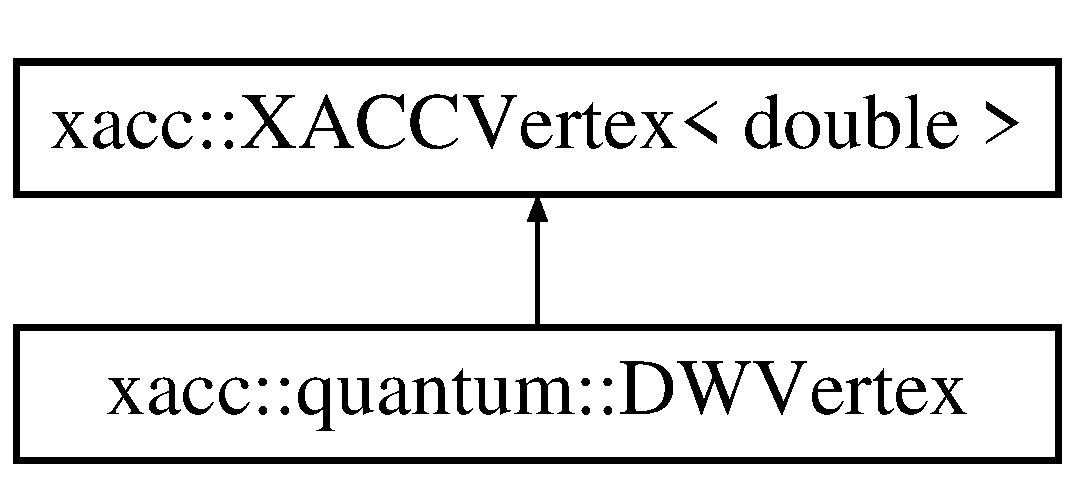
\includegraphics[height=2.000000cm]{a00049}
\end{center}
\end{figure}
\subsection*{Public Member Functions}
\begin{DoxyCompactItemize}
\item 
virtual std\+::shared\+\_\+ptr$<$ \hyperlink{a00038}{Function} $>$ \hyperlink{a00049_af42e466bf02dbd60670d20aa55cfb08d}{generate\+Algorithm} (std\+::vector$<$ int $>$ qubits)
\item 
virtual \hyperlink{a00049_a731c10d28046424be74e4c0daa31d016}{$\sim$\+Inverse\+Q\+FT} ()
\end{DoxyCompactItemize}


\subsection{Detailed Description}
\hyperlink{a00049}{Inverse\+Q\+FT} is a realization of the \hyperlink{a00014}{Algorithm\+Generator} interface that produces an X\+A\+CC \hyperlink{a00050}{IR} representation of the Inverse Quantum Fourier Transform. 

\subsection{Constructor \& Destructor Documentation}
\index{xacc\+::quantum\+::\+Inverse\+Q\+FT@{xacc\+::quantum\+::\+Inverse\+Q\+FT}!````~Inverse\+Q\+FT@{$\sim$\+Inverse\+Q\+FT}}
\index{````~Inverse\+Q\+FT@{$\sim$\+Inverse\+Q\+FT}!xacc\+::quantum\+::\+Inverse\+Q\+FT@{xacc\+::quantum\+::\+Inverse\+Q\+FT}}
\subsubsection[{\texorpdfstring{$\sim$\+Inverse\+Q\+F\+T()}{~InverseQFT()}}]{\setlength{\rightskip}{0pt plus 5cm}virtual xacc\+::quantum\+::\+Inverse\+Q\+F\+T\+::$\sim$\+Inverse\+Q\+FT (
\begin{DoxyParamCaption}
{}
\end{DoxyParamCaption}
)\hspace{0.3cm}{\ttfamily [inline]}, {\ttfamily [virtual]}}\hypertarget{a00049_a731c10d28046424be74e4c0daa31d016}{}\label{a00049_a731c10d28046424be74e4c0daa31d016}
The destructor 

\subsection{Member Function Documentation}
\index{xacc\+::quantum\+::\+Inverse\+Q\+FT@{xacc\+::quantum\+::\+Inverse\+Q\+FT}!generate\+Algorithm@{generate\+Algorithm}}
\index{generate\+Algorithm@{generate\+Algorithm}!xacc\+::quantum\+::\+Inverse\+Q\+FT@{xacc\+::quantum\+::\+Inverse\+Q\+FT}}
\subsubsection[{\texorpdfstring{generate\+Algorithm(std\+::vector$<$ int $>$ qubits)}{generateAlgorithm(std::vector< int > qubits)}}]{\setlength{\rightskip}{0pt plus 5cm}std\+::shared\+\_\+ptr$<$ {\bf Function} $>$ xacc\+::quantum\+::\+Inverse\+Q\+F\+T\+::generate\+Algorithm (
\begin{DoxyParamCaption}
\item[{std\+::vector$<$ int $>$}]{qubits}
\end{DoxyParamCaption}
)\hspace{0.3cm}{\ttfamily [virtual]}}\hypertarget{a00049_af42e466bf02dbd60670d20aa55cfb08d}{}\label{a00049_af42e466bf02dbd60670d20aa55cfb08d}
This implementation returns a \hyperlink{a00038}{Function} \hyperlink{a00050}{IR} representation of the inverse quantum fourier transform.


\begin{DoxyParams}{Parameters}
{\em bits} & The bits this algorithm operates on \\
\hline
\end{DoxyParams}
\begin{DoxyReturn}{Returns}
function The algorithm represented as an \hyperlink{a00050}{IR} \hyperlink{a00038}{Function} 
\end{DoxyReturn}


Implements \hyperlink{a00014_a73023c06f0f0c62ad56ab4187b18b096}{xacc\+::\+Algorithm\+Generator}.



The documentation for this class was generated from the following files\+:\begin{DoxyCompactItemize}
\item 
Inverse\+Q\+F\+T.\+hpp\item 
Inverse\+Q\+F\+T.\+cpp\end{DoxyCompactItemize}

\hypertarget{a00050}{}\section{case\+\_\+insensitive\+\_\+equals Class Reference}
\label{a00050}\index{case\+\_\+insensitive\+\_\+equals@{case\+\_\+insensitive\+\_\+equals}}
\subsection*{Public Member Functions}
\begin{DoxyCompactItemize}
\item 
bool {\bfseries operator()} (const std\+::string \&key1, const std\+::string \&key2) const \hypertarget{a00050_a4110d72a3ecfd3bd8ab698dd13c877d3}{}\label{a00050_a4110d72a3ecfd3bd8ab698dd13c877d3}

\item 
bool {\bfseries operator()} (const std\+::string \&key1, const std\+::string \&key2) const \hypertarget{a00050_a4110d72a3ecfd3bd8ab698dd13c877d3}{}\label{a00050_a4110d72a3ecfd3bd8ab698dd13c877d3}

\end{DoxyCompactItemize}


The documentation for this class was generated from the following files\+:\begin{DoxyCompactItemize}
\item 
client\+\_\+http.\+hpp\item 
server\+\_\+http.\+hpp\end{DoxyCompactItemize}

\hypertarget{a00051}{}\section{case\+\_\+insensitive\+\_\+hash Class Reference}
\label{a00051}\index{case\+\_\+insensitive\+\_\+hash@{case\+\_\+insensitive\+\_\+hash}}
\subsection*{Public Member Functions}
\begin{DoxyCompactItemize}
\item 
std\+::size\+\_\+t {\bfseries operator()} (const std\+::string \&key) const \hypertarget{a00051_a9969b2f956909125d5a83864a15736f4}{}\label{a00051_a9969b2f956909125d5a83864a15736f4}

\item 
size\+\_\+t {\bfseries operator()} (const std\+::string \&key) const \hypertarget{a00051_a1c9bbdf416c7580c3f9716abf5269746}{}\label{a00051_a1c9bbdf416c7580c3f9716abf5269746}

\end{DoxyCompactItemize}


The documentation for this class was generated from the following files\+:\begin{DoxyCompactItemize}
\item 
client\+\_\+http.\+hpp\item 
server\+\_\+http.\+hpp\end{DoxyCompactItemize}

\hypertarget{a00052}{}\section{xacc\+:\+:quantum\+:\+:Embedding\+Algorithm Class Reference}
\label{a00052}\index{xacc\+::quantum\+::\+Embedding\+Algorithm@{xacc\+::quantum\+::\+Embedding\+Algorithm}}


{\ttfamily \#include $<$Embedding\+Algorithm.\+hpp$>$}

Inheritance diagram for xacc\+:\+:quantum\+:\+:Embedding\+Algorithm\+:\begin{figure}[H]
\begin{center}
\leavevmode
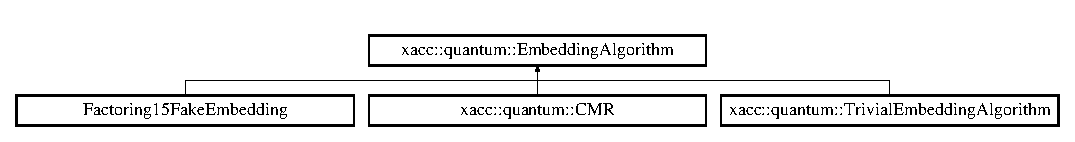
\includegraphics[height=1.464052cm]{a00052}
\end{center}
\end{figure}
\subsection*{Public Member Functions}
\begin{DoxyCompactItemize}
\item 
\hyperlink{a00052_abad06507eef6b63af0884e3a96145c69}{Embedding\+Algorithm} ()
\item 
virtual \hyperlink{a00052_aa43660ad5d4c4b3ac67863892c33dc51}{$\sim$\+Embedding\+Algorithm} ()
\item 
virtual std\+::map$<$ int, std\+::list$<$ int $>$ $>$ \hyperlink{a00052_a6fca277e217884ff79802770189276fe}{embed} (std\+::shared\+\_\+ptr$<$ \hyperlink{a00043}{D\+W\+Graph} $>$ problem, std\+::shared\+\_\+ptr$<$ \hyperlink{a00064}{Accelerator\+Graph} $>$ hardware, std\+::map$<$ std\+::string, std\+::string $>$ params=std\+::map$<$ std\+::string, std\+::string $>$())=0
\item 
virtual std\+::string \hyperlink{a00052_a21079dc8ee37792977f5fd209e3f3b19}{name} ()=0
\end{DoxyCompactItemize}


\subsection{Detailed Description}
The \hyperlink{a00052}{Embedding\+Algorithm} class provides an interface for minor graph embedding algorithms. 

\subsection{Constructor \& Destructor Documentation}
\index{xacc\+::quantum\+::\+Embedding\+Algorithm@{xacc\+::quantum\+::\+Embedding\+Algorithm}!Embedding\+Algorithm@{Embedding\+Algorithm}}
\index{Embedding\+Algorithm@{Embedding\+Algorithm}!xacc\+::quantum\+::\+Embedding\+Algorithm@{xacc\+::quantum\+::\+Embedding\+Algorithm}}
\subsubsection[{\texorpdfstring{Embedding\+Algorithm()}{EmbeddingAlgorithm()}}]{\setlength{\rightskip}{0pt plus 5cm}xacc\+::quantum\+::\+Embedding\+Algorithm\+::\+Embedding\+Algorithm (
\begin{DoxyParamCaption}
{}
\end{DoxyParamCaption}
)\hspace{0.3cm}{\ttfamily [inline]}}\hypertarget{a00052_abad06507eef6b63af0884e3a96145c69}{}\label{a00052_abad06507eef6b63af0884e3a96145c69}
The Constructor \index{xacc\+::quantum\+::\+Embedding\+Algorithm@{xacc\+::quantum\+::\+Embedding\+Algorithm}!````~Embedding\+Algorithm@{$\sim$\+Embedding\+Algorithm}}
\index{````~Embedding\+Algorithm@{$\sim$\+Embedding\+Algorithm}!xacc\+::quantum\+::\+Embedding\+Algorithm@{xacc\+::quantum\+::\+Embedding\+Algorithm}}
\subsubsection[{\texorpdfstring{$\sim$\+Embedding\+Algorithm()}{~EmbeddingAlgorithm()}}]{\setlength{\rightskip}{0pt plus 5cm}virtual xacc\+::quantum\+::\+Embedding\+Algorithm\+::$\sim$\+Embedding\+Algorithm (
\begin{DoxyParamCaption}
{}
\end{DoxyParamCaption}
)\hspace{0.3cm}{\ttfamily [inline]}, {\ttfamily [virtual]}}\hypertarget{a00052_aa43660ad5d4c4b3ac67863892c33dc51}{}\label{a00052_aa43660ad5d4c4b3ac67863892c33dc51}
The Destructor 

\subsection{Member Function Documentation}
\index{xacc\+::quantum\+::\+Embedding\+Algorithm@{xacc\+::quantum\+::\+Embedding\+Algorithm}!embed@{embed}}
\index{embed@{embed}!xacc\+::quantum\+::\+Embedding\+Algorithm@{xacc\+::quantum\+::\+Embedding\+Algorithm}}
\subsubsection[{\texorpdfstring{embed(std\+::shared\+\_\+ptr$<$ D\+W\+Graph $>$ problem, std\+::shared\+\_\+ptr$<$ Accelerator\+Graph $>$ hardware, std\+::map$<$ std\+::string, std\+::string $>$ params=std\+::map$<$ std\+::string, std\+::string $>$())=0}{embed(std::shared\_ptr< DWGraph > problem, std::shared\_ptr< AcceleratorGraph > hardware, std::map< std::string, std::string > params=std::map< std::string, std::string >())=0}}]{\setlength{\rightskip}{0pt plus 5cm}virtual std\+::map$<$int, std\+::list$<$int$>$ $>$ xacc\+::quantum\+::\+Embedding\+Algorithm\+::embed (
\begin{DoxyParamCaption}
\item[{std\+::shared\+\_\+ptr$<$ {\bf D\+W\+Graph} $>$}]{problem, }
\item[{std\+::shared\+\_\+ptr$<$ {\bf Accelerator\+Graph} $>$}]{hardware, }
\item[{std\+::map$<$ std\+::string, std\+::string $>$}]{params = {\ttfamily std\+:\+:map$<$~std\+:\+:string,~std\+:\+:string~$>$()}}
\end{DoxyParamCaption}
)\hspace{0.3cm}{\ttfamily [pure virtual]}}\hypertarget{a00052_a6fca277e217884ff79802770189276fe}{}\label{a00052_a6fca277e217884ff79802770189276fe}
Implementations of \hyperlink{a00052}{Embedding\+Algorithm} implement this method to provide a valid minor graph embedding of the given problem graph into the given hardware graph.


\begin{DoxyParams}{Parameters}
{\em problem} & The problem graph to be embedded into the hardware graph \\
\hline
{\em hardware} & The hardware graph. \\
\hline
{\em params} & Any key-\/value string parameters to influence the algorithm. \\
\hline
\end{DoxyParams}
\begin{DoxyReturn}{Returns}
embedding A mapping of problem vertex indices to the list of hardware vertices they map to 
\end{DoxyReturn}


Implemented in \hyperlink{a00127_a09e162a745528ffa3ea847dd5afee45b}{xacc\+::quantum\+::\+Trivial\+Embedding\+Algorithm}, and \hyperlink{a00032_a3408b5b72c426b4733ea4b0a19feb2f4}{xacc\+::quantum\+::\+C\+MR}.

\index{xacc\+::quantum\+::\+Embedding\+Algorithm@{xacc\+::quantum\+::\+Embedding\+Algorithm}!name@{name}}
\index{name@{name}!xacc\+::quantum\+::\+Embedding\+Algorithm@{xacc\+::quantum\+::\+Embedding\+Algorithm}}
\subsubsection[{\texorpdfstring{name()=0}{name()=0}}]{\setlength{\rightskip}{0pt plus 5cm}virtual std\+::string xacc\+::quantum\+::\+Embedding\+Algorithm\+::name (
\begin{DoxyParamCaption}
{}
\end{DoxyParamCaption}
)\hspace{0.3cm}{\ttfamily [pure virtual]}}\hypertarget{a00052_a21079dc8ee37792977f5fd209e3f3b19}{}\label{a00052_a21079dc8ee37792977f5fd209e3f3b19}
Return the name of this \hyperlink{a00051}{Embedding} Algorithm \begin{DoxyReturn}{Returns}

\end{DoxyReturn}


Implemented in \hyperlink{a00058_a2fc78d2c2960cb0900b9224c8a2baf61}{Factoring15\+Fake\+Embedding}, \hyperlink{a00127_a5d3e8c56b53cda9c682dedc534bf38fb}{xacc\+::quantum\+::\+Trivial\+Embedding\+Algorithm}, and \hyperlink{a00032_a06abf96899ccbfb4e2e0b2c72f978854}{xacc\+::quantum\+::\+C\+MR}.



The documentation for this class was generated from the following file\+:\begin{DoxyCompactItemize}
\item 
Embedding\+Algorithm.\+hpp\end{DoxyCompactItemize}

\hypertarget{a00053}{}\section{Embedding\+Algorithm\+Factory Class Reference}
\label{a00053}\index{Embedding\+Algorithm\+Factory@{Embedding\+Algorithm\+Factory}}


{\ttfamily \#include $<$Embedding\+Algorithm\+Factory.\+hpp$>$}

\subsection*{Public Member Functions}
\begin{DoxyCompactItemize}
\item 
std\+::shared\+\_\+ptr$<$ \hyperlink{a00071}{I\+Embedding\+Algorithm} $>$ \hyperlink{a00053_a19e9ec2636073705e65c1039c8879be7}{create\+Embedding\+Algorithm} (std\+::string type, \hyperlink{a00076}{I\+Quell\+E\+Graph} \&prob, \hyperlink{a00076}{I\+Quell\+E\+Graph} \&hardware)
\item 
{\footnotesize template$<$typename T $>$ }\\void \hyperlink{a00053_aec39e8d4edc3715f3980db5d13252f3b}{reg} (const std\+::string \&name)
\item 
std\+::vector$<$ std\+::string $>$ {\bfseries list\+Embedding\+Algorithms} ()\hypertarget{a00053_ab19e4f507f0ac05a0b37ae75c68b6df4}{}\label{a00053_ab19e4f507f0ac05a0b37ae75c68b6df4}

\end{DoxyCompactItemize}
\subsection*{Static Public Member Functions}
\begin{DoxyCompactItemize}
\item 
static std\+::shared\+\_\+ptr$<$ \hyperlink{a00053}{Embedding\+Algorithm\+Factory} $>$ \hyperlink{a00053_a1fccee9971df2df4870cd1333798b3da}{instance} ()
\end{DoxyCompactItemize}
\subsection*{Protected Member Functions}
\begin{DoxyCompactItemize}
\item 
\hyperlink{a00053_ac19af2c293caa47ea46a0122f3e81e28}{Embedding\+Algorithm\+Factory} ()
\end{DoxyCompactItemize}
\subsection*{Protected Attributes}
\begin{DoxyCompactItemize}
\item 
std\+::map$<$ std\+::string, build\+Ptr $>$ \hyperlink{a00053_aa3bbf5d1683ddd7194f981f0af67e95a}{registration\+Map}
\end{DoxyCompactItemize}
\subsection*{Static Protected Attributes}
\begin{DoxyCompactItemize}
\item 
static std\+::shared\+\_\+ptr$<$ \hyperlink{a00053}{Embedding\+Algorithm\+Factory} $>$ \hyperlink{a00053_ad675ae385b8ffb8fb4eafe0253967ed9}{factory\+Instance} = 0
\end{DoxyCompactItemize}


\subsection{Detailed Description}
The \hyperlink{a00053}{Embedding\+Algorithm\+Factory} is a singleton that dynamically registers I\+Embedding\+Algorithms and provides a mechanism for clients to create them by just knowing the string name of the class. 

\subsection{Constructor \& Destructor Documentation}
\index{Embedding\+Algorithm\+Factory@{Embedding\+Algorithm\+Factory}!Embedding\+Algorithm\+Factory@{Embedding\+Algorithm\+Factory}}
\index{Embedding\+Algorithm\+Factory@{Embedding\+Algorithm\+Factory}!Embedding\+Algorithm\+Factory@{Embedding\+Algorithm\+Factory}}
\subsubsection[{\texorpdfstring{Embedding\+Algorithm\+Factory()}{EmbeddingAlgorithmFactory()}}]{\setlength{\rightskip}{0pt plus 5cm}Embedding\+Algorithm\+Factory\+::\+Embedding\+Algorithm\+Factory (
\begin{DoxyParamCaption}
{}
\end{DoxyParamCaption}
)\hspace{0.3cm}{\ttfamily [inline]}, {\ttfamily [protected]}}\hypertarget{a00053_ac19af2c293caa47ea46a0122f3e81e28}{}\label{a00053_ac19af2c293caa47ea46a0122f3e81e28}
The Constructor 

\subsection{Member Function Documentation}
\index{Embedding\+Algorithm\+Factory@{Embedding\+Algorithm\+Factory}!create\+Embedding\+Algorithm@{create\+Embedding\+Algorithm}}
\index{create\+Embedding\+Algorithm@{create\+Embedding\+Algorithm}!Embedding\+Algorithm\+Factory@{Embedding\+Algorithm\+Factory}}
\subsubsection[{\texorpdfstring{create\+Embedding\+Algorithm(std\+::string type, I\+Quell\+E\+Graph \&prob, I\+Quell\+E\+Graph \&hardware)}{createEmbeddingAlgorithm(std::string type, IQuellEGraph \&prob, IQuellEGraph \&hardware)}}]{\setlength{\rightskip}{0pt plus 5cm}std\+::shared\+\_\+ptr$<${\bf I\+Embedding\+Algorithm}$>$ Embedding\+Algorithm\+Factory\+::create\+Embedding\+Algorithm (
\begin{DoxyParamCaption}
\item[{std\+::string}]{type, }
\item[{{\bf I\+Quell\+E\+Graph} \&}]{prob, }
\item[{{\bf I\+Quell\+E\+Graph} \&}]{hardware}
\end{DoxyParamCaption}
)\hspace{0.3cm}{\ttfamily [inline]}}\hypertarget{a00053_a19e9ec2636073705e65c1039c8879be7}{}\label{a00053_a19e9ec2636073705e65c1039c8879be7}
Create the \hyperlink{a00071}{I\+Embedding\+Algorithm} corresponding to the provided string type and problem/hardware graphs.


\begin{DoxyParams}{Parameters}
{\em type} & \\
\hline
{\em prob} & \\
\hline
{\em hardware} & \\
\hline
\end{DoxyParams}
\begin{DoxyReturn}{Returns}

\end{DoxyReturn}
\index{Embedding\+Algorithm\+Factory@{Embedding\+Algorithm\+Factory}!instance@{instance}}
\index{instance@{instance}!Embedding\+Algorithm\+Factory@{Embedding\+Algorithm\+Factory}}
\subsubsection[{\texorpdfstring{instance()}{instance()}}]{\setlength{\rightskip}{0pt plus 5cm}static std\+::shared\+\_\+ptr$<${\bf Embedding\+Algorithm\+Factory}$>$ Embedding\+Algorithm\+Factory\+::instance (
\begin{DoxyParamCaption}
{}
\end{DoxyParamCaption}
)\hspace{0.3cm}{\ttfamily [inline]}, {\ttfamily [static]}}\hypertarget{a00053_a1fccee9971df2df4870cd1333798b3da}{}\label{a00053_a1fccee9971df2df4870cd1333798b3da}
Return the singleton instance for this factory.

\begin{DoxyReturn}{Returns}

\end{DoxyReturn}
\index{Embedding\+Algorithm\+Factory@{Embedding\+Algorithm\+Factory}!reg@{reg}}
\index{reg@{reg}!Embedding\+Algorithm\+Factory@{Embedding\+Algorithm\+Factory}}
\subsubsection[{\texorpdfstring{reg(const std\+::string \&name)}{reg(const std::string \&name)}}]{\setlength{\rightskip}{0pt plus 5cm}template$<$typename T $>$ void Embedding\+Algorithm\+Factory\+::reg (
\begin{DoxyParamCaption}
\item[{const std\+::string \&}]{name}
\end{DoxyParamCaption}
)\hspace{0.3cm}{\ttfamily [inline]}}\hypertarget{a00053_aec39e8d4edc3715f3980db5d13252f3b}{}\label{a00053_aec39e8d4edc3715f3980db5d13252f3b}
Register a new \hyperlink{a00071}{I\+Embedding\+Algorithm} with the factory.


\begin{DoxyParams}{Parameters}
{\em name} & \\
\hline
\end{DoxyParams}


\subsection{Member Data Documentation}
\index{Embedding\+Algorithm\+Factory@{Embedding\+Algorithm\+Factory}!factory\+Instance@{factory\+Instance}}
\index{factory\+Instance@{factory\+Instance}!Embedding\+Algorithm\+Factory@{Embedding\+Algorithm\+Factory}}
\subsubsection[{\texorpdfstring{factory\+Instance}{factoryInstance}}]{\setlength{\rightskip}{0pt plus 5cm}std\+::shared\+\_\+ptr$<$ {\bf Embedding\+Algorithm\+Factory} $>$ Embedding\+Algorithm\+Factory\+::factory\+Instance = 0\hspace{0.3cm}{\ttfamily [static]}, {\ttfamily [protected]}}\hypertarget{a00053_ad675ae385b8ffb8fb4eafe0253967ed9}{}\label{a00053_ad675ae385b8ffb8fb4eafe0253967ed9}
Reference to the singleton instance \index{Embedding\+Algorithm\+Factory@{Embedding\+Algorithm\+Factory}!registration\+Map@{registration\+Map}}
\index{registration\+Map@{registration\+Map}!Embedding\+Algorithm\+Factory@{Embedding\+Algorithm\+Factory}}
\subsubsection[{\texorpdfstring{registration\+Map}{registrationMap}}]{\setlength{\rightskip}{0pt plus 5cm}std\+::map$<$std\+::string, build\+Ptr$>$ Embedding\+Algorithm\+Factory\+::registration\+Map\hspace{0.3cm}{\ttfamily [protected]}}\hypertarget{a00053_aa3bbf5d1683ddd7194f981f0af67e95a}{}\label{a00053_aa3bbf5d1683ddd7194f981f0af67e95a}
Reference to the registration map. 

The documentation for this class was generated from the following files\+:\begin{DoxyCompactItemize}
\item 
Embedding\+Algorithm\+Factory.\+hpp\item 
Embedding\+Algorithm\+Factory.\+cpp\end{DoxyCompactItemize}

\hypertarget{a00054}{}\section{xacc\+:\+:quantum\+:\+:K44\+Bipartite Class Reference}
\label{a00054}\index{xacc\+::quantum\+::\+K44\+Bipartite@{xacc\+::quantum\+::\+K44\+Bipartite}}
Inheritance diagram for xacc\+:\+:quantum\+:\+:K44\+Bipartite\+:\begin{figure}[H]
\begin{center}
\leavevmode
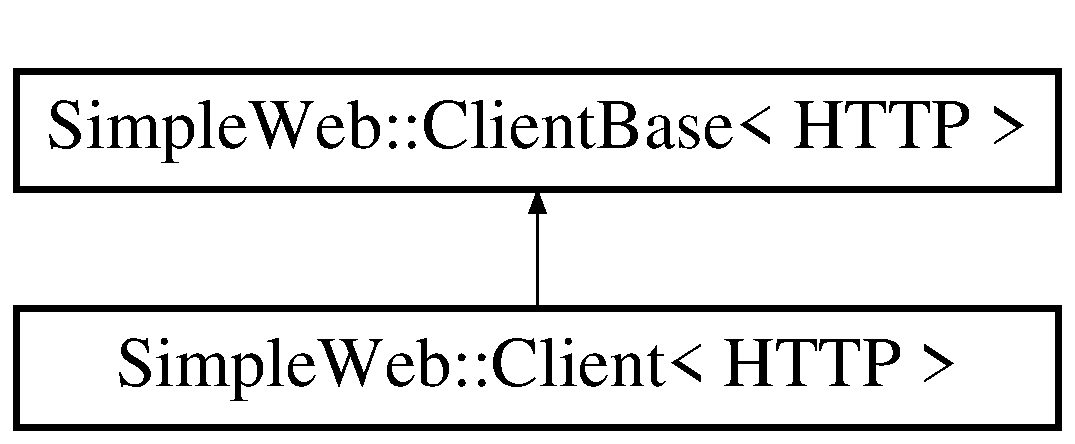
\includegraphics[height=3.000000cm]{a00054}
\end{center}
\end{figure}
\subsection*{Additional Inherited Members}


The documentation for this class was generated from the following file\+:\begin{DoxyCompactItemize}
\item 
D\+W\+Graph.\+hpp\end{DoxyCompactItemize}

\hypertarget{a00055}{}\section{xacc\+:\+:quantum\+:\+:Register\+Gate\+Instruction$<$ T $>$ Class Template Reference}
\label{a00055}\index{xacc\+::quantum\+::\+Register\+Gate\+Instruction$<$ T $>$@{xacc\+::quantum\+::\+Register\+Gate\+Instruction$<$ T $>$}}
\subsection*{Public Member Functions}
\begin{DoxyCompactItemize}
\item 
{\bfseries Register\+Gate\+Instruction} (const std\+::string \&name)\hypertarget{a00055_aad394924e098f0cc8da5cc7f211acd7a}{}\label{a00055_aad394924e098f0cc8da5cc7f211acd7a}

\end{DoxyCompactItemize}


The documentation for this class was generated from the following file\+:\begin{DoxyCompactItemize}
\item 
Gate\+Instruction.\+hpp\end{DoxyCompactItemize}

\hypertarget{a00056}{}\section{xacc\+:\+:Registry$<$ T, T\+Args $>$ Class Template Reference}
\label{a00056}\index{xacc\+::\+Registry$<$ T, T\+Args $>$@{xacc\+::\+Registry$<$ T, T\+Args $>$}}


{\ttfamily \#include $<$Registry.\+hpp$>$}

Inheritance diagram for xacc\+:\+:Registry$<$ T, T\+Args $>$\+:\begin{figure}[H]
\begin{center}
\leavevmode
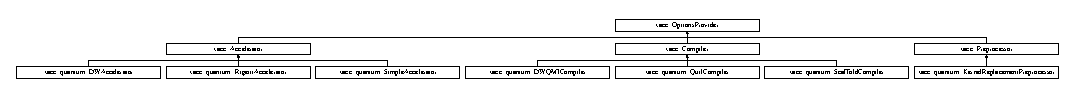
\includegraphics[height=2.000000cm]{a00056}
\end{center}
\end{figure}
\subsection*{Public Member Functions}
\begin{DoxyCompactItemize}
\item 
bool \hyperlink{a00056_a9aa172c2603171db067b40bd62ba53c6}{add} (const std\+::string \&id, std\+::function$<$ std\+::shared\+\_\+ptr$<$ T $>$(T\+Args...)$>$ f)
\item 
std\+::shared\+\_\+ptr$<$ T $>$ \hyperlink{a00056_aecccbd5534276cbdd1553e43c942219b}{create} (const std\+::string \&id, T\+Args...\+args)
\item 
std\+::vector$<$ std\+::string $>$ \hyperlink{a00056_a8bff6f5c50534375abc4026662d69d2e}{get\+Registered\+Ids} ()
\item 
std\+::size\+\_\+t \hyperlink{a00056_a2352dd7c6c85ae5c5e232b577dfa2544}{size} ()
\end{DoxyCompactItemize}
\subsection*{Protected Attributes}
\begin{DoxyCompactItemize}
\item 
std\+::map$<$ std\+::string, std\+::function$<$ std\+::shared\+\_\+ptr$<$ T $>$T\+Args...)$>$ $>$ \hyperlink{a00056_a46460ecacc7facb6936b3c1ec6d618d7}{registry}
\end{DoxyCompactItemize}
\subsection*{Additional Inherited Members}


\subsection{Detailed Description}
\subsubsection*{template$<$typename T, typename... T\+Args$>$\\*
class xacc\+::\+Registry$<$ T, T\+Args $>$}

\hyperlink{a00056}{Registry} is a \hyperlink{a00068}{Singleton} that provides a mapping of string ids to creation functions that create and return the provided \hyperlink{a00056}{Registry} template parameter T.

Clients can add new creation functions to be placed in the map with a unique name key, and can request that the \hyperlink{a00056}{Registry} return a new created instance of the template parameter T. 

\subsection{Member Function Documentation}
\index{xacc\+::\+Registry@{xacc\+::\+Registry}!add@{add}}
\index{add@{add}!xacc\+::\+Registry@{xacc\+::\+Registry}}
\subsubsection[{\texorpdfstring{add(const std\+::string \&id, std\+::function$<$ std\+::shared\+\_\+ptr$<$ T $>$(\+T\+Args...)$>$ f)}{add(const std::string \&id, std::function< std::shared\_ptr< T >(TArgs...)> f)}}]{\setlength{\rightskip}{0pt plus 5cm}template$<$typename T, typename... T\+Args$>$ bool {\bf xacc\+::\+Registry}$<$ T, T\+Args $>$\+::add (
\begin{DoxyParamCaption}
\item[{const std\+::string \&}]{id, }
\item[{std\+::function$<$ std\+::shared\+\_\+ptr$<$ T $>$(T\+Args...)$>$}]{f}
\end{DoxyParamCaption}
)\hspace{0.3cm}{\ttfamily [inline]}}\hypertarget{a00056_a9aa172c2603171db067b40bd62ba53c6}{}\label{a00056_a9aa172c2603171db067b40bd62ba53c6}
Add a new creation function to the \hyperlink{a00056}{Registry}, keyed on the provided string id.


\begin{DoxyParams}{Parameters}
{\em id} & The Id of the creation function \\
\hline
{\em f} & The object\textquotesingle{}s creation function \\
\hline
\end{DoxyParams}
\begin{DoxyReturn}{Returns}
success Bool indicating if this creator was added successfully. 
\end{DoxyReturn}
\index{xacc\+::\+Registry@{xacc\+::\+Registry}!create@{create}}
\index{create@{create}!xacc\+::\+Registry@{xacc\+::\+Registry}}
\subsubsection[{\texorpdfstring{create(const std\+::string \&id, T\+Args...\+args)}{create(const std::string \&id, TArgs...args)}}]{\setlength{\rightskip}{0pt plus 5cm}template$<$typename T, typename... T\+Args$>$ std\+::shared\+\_\+ptr$<$T$>$ {\bf xacc\+::\+Registry}$<$ T, T\+Args $>$\+::create (
\begin{DoxyParamCaption}
\item[{const std\+::string \&}]{id, }
\item[{T\+Args...}]{args}
\end{DoxyParamCaption}
)\hspace{0.3cm}{\ttfamily [inline]}}\hypertarget{a00056_aecccbd5534276cbdd1553e43c942219b}{}\label{a00056_aecccbd5534276cbdd1553e43c942219b}
Create an instance of T by using the creation function found at the given key string id.


\begin{DoxyParams}{Parameters}
{\em id} & The Id of the creation function \\
\hline
\end{DoxyParams}
\begin{DoxyReturn}{Returns}
object Shared Pointer for the created object. 
\end{DoxyReturn}
\index{xacc\+::\+Registry@{xacc\+::\+Registry}!get\+Registered\+Ids@{get\+Registered\+Ids}}
\index{get\+Registered\+Ids@{get\+Registered\+Ids}!xacc\+::\+Registry@{xacc\+::\+Registry}}
\subsubsection[{\texorpdfstring{get\+Registered\+Ids()}{getRegisteredIds()}}]{\setlength{\rightskip}{0pt plus 5cm}template$<$typename T, typename... T\+Args$>$ std\+::vector$<$std\+::string$>$ {\bf xacc\+::\+Registry}$<$ T, T\+Args $>$\+::get\+Registered\+Ids (
\begin{DoxyParamCaption}
{}
\end{DoxyParamCaption}
)\hspace{0.3cm}{\ttfamily [inline]}}\hypertarget{a00056_a8bff6f5c50534375abc4026662d69d2e}{}\label{a00056_a8bff6f5c50534375abc4026662d69d2e}
Return the keys from the registry map.

\begin{DoxyReturn}{Returns}
ids The registered creator Ids 
\end{DoxyReturn}
\index{xacc\+::\+Registry@{xacc\+::\+Registry}!size@{size}}
\index{size@{size}!xacc\+::\+Registry@{xacc\+::\+Registry}}
\subsubsection[{\texorpdfstring{size()}{size()}}]{\setlength{\rightskip}{0pt plus 5cm}template$<$typename T, typename... T\+Args$>$ std\+::size\+\_\+t {\bf xacc\+::\+Registry}$<$ T, T\+Args $>$\+::size (
\begin{DoxyParamCaption}
{}
\end{DoxyParamCaption}
)\hspace{0.3cm}{\ttfamily [inline]}}\hypertarget{a00056_a2352dd7c6c85ae5c5e232b577dfa2544}{}\label{a00056_a2352dd7c6c85ae5c5e232b577dfa2544}
Return the number of creation functions this registry contains.

\begin{DoxyReturn}{Returns}
size The number of creators in this \hyperlink{a00056}{Registry} 
\end{DoxyReturn}


\subsection{Member Data Documentation}
\index{xacc\+::\+Registry@{xacc\+::\+Registry}!registry@{registry}}
\index{registry@{registry}!xacc\+::\+Registry@{xacc\+::\+Registry}}
\subsubsection[{\texorpdfstring{registry}{registry}}]{\setlength{\rightskip}{0pt plus 5cm}template$<$typename T, typename... T\+Args$>$ std\+::map$<$std\+::string, std\+::function$<$std\+::shared\+\_\+ptr$<$T$>$T\+Args...)$>$ $>$ {\bf xacc\+::\+Registry}$<$ T, T\+Args $>$\+::registry\hspace{0.3cm}{\ttfamily [protected]}}\hypertarget{a00056_a46460ecacc7facb6936b3c1ec6d618d7}{}\label{a00056_a46460ecacc7facb6936b3c1ec6d618d7}
Reference to the database of creation functions for classes of superclass type T. 

The documentation for this class was generated from the following file\+:\begin{DoxyCompactItemize}
\item 
Registry.\+hpp\end{DoxyCompactItemize}

\hypertarget{a00057}{}\section{xacc\+:\+:Options\+Provider Class Reference}
\label{a00057}\index{xacc\+::\+Options\+Provider@{xacc\+::\+Options\+Provider}}


{\ttfamily \#include $<$Options\+Provider.\+hpp$>$}

Inheritance diagram for xacc\+:\+:Options\+Provider\+:\begin{figure}[H]
\begin{center}
\leavevmode
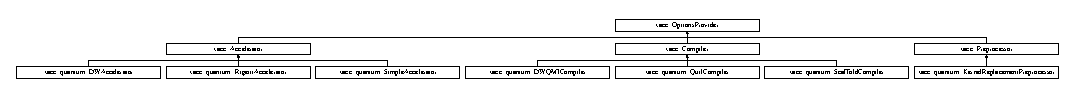
\includegraphics[height=0.824742cm]{a00057}
\end{center}
\end{figure}
\subsection*{Public Member Functions}
\begin{DoxyCompactItemize}
\item 
virtual std\+::shared\+\_\+ptr$<$ options\+\_\+description $>$ \hyperlink{a00057_a6d150954f852109bfe2c1ae90222926f}{get\+Options} ()=0
\item 
virtual \hyperlink{a00057_a7782757b419792ff346f563517eed8b8}{$\sim$\+Options\+Provider} ()
\end{DoxyCompactItemize}


\subsection{Detailed Description}
The \hyperlink{a00057}{Options\+Provider} interface enables derived subclasses to provide a description of any and all command line options that they can take to drive and control their execution and behavior. 

\subsection{Constructor \& Destructor Documentation}
\index{xacc\+::\+Options\+Provider@{xacc\+::\+Options\+Provider}!````~Options\+Provider@{$\sim$\+Options\+Provider}}
\index{````~Options\+Provider@{$\sim$\+Options\+Provider}!xacc\+::\+Options\+Provider@{xacc\+::\+Options\+Provider}}
\subsubsection[{\texorpdfstring{$\sim$\+Options\+Provider()}{~OptionsProvider()}}]{\setlength{\rightskip}{0pt plus 5cm}virtual xacc\+::\+Options\+Provider\+::$\sim$\+Options\+Provider (
\begin{DoxyParamCaption}
{}
\end{DoxyParamCaption}
)\hspace{0.3cm}{\ttfamily [inline]}, {\ttfamily [virtual]}}\hypertarget{a00057_a7782757b419792ff346f563517eed8b8}{}\label{a00057_a7782757b419792ff346f563517eed8b8}
The destructor 

\subsection{Member Function Documentation}
\index{xacc\+::\+Options\+Provider@{xacc\+::\+Options\+Provider}!get\+Options@{get\+Options}}
\index{get\+Options@{get\+Options}!xacc\+::\+Options\+Provider@{xacc\+::\+Options\+Provider}}
\subsubsection[{\texorpdfstring{get\+Options()=0}{getOptions()=0}}]{\setlength{\rightskip}{0pt plus 5cm}virtual std\+::shared\+\_\+ptr$<$options\+\_\+description$>$ xacc\+::\+Options\+Provider\+::get\+Options (
\begin{DoxyParamCaption}
{}
\end{DoxyParamCaption}
)\hspace{0.3cm}{\ttfamily [pure virtual]}}\hypertarget{a00057_a6d150954f852109bfe2c1ae90222926f}{}\label{a00057_a6d150954f852109bfe2c1ae90222926f}
Return a Boost options\+\_\+description instance that describes the options available for this derived subclass. 

Implemented in \hyperlink{a00011_a98c9eda6b54367c75667ecfbbf167979}{xacc\+::\+Accelerator}, \hyperlink{a00029_a09926db9f99706307ae6ce5b56845bca}{xacc\+::quantum\+::\+D\+W\+Accelerator}, \hyperlink{a00072_a9ee9e62aecbccf193894ca3388676f9f}{xacc\+::quantum\+::\+Rigetti\+Accelerator}, \hyperlink{a00023_a9f5a8965c9c2dd895016d18264ebbe92}{xacc\+::\+Compiler}, \hyperlink{a00034_a0851334cc33b5b1da2694150a0a1a43c}{xacc\+::quantum\+::\+D\+W\+Q\+M\+I\+Compiler}, and \hyperlink{a00058_a96f5600ea47628b66917c7b90250e7f1}{xacc\+::\+Preprocessor}.



The documentation for this class was generated from the following file\+:\begin{DoxyCompactItemize}
\item 
Options\+Provider.\+hpp\end{DoxyCompactItemize}

\hypertarget{a00058}{}\section{xacc\+:\+:Program Class Reference}
\label{a00058}\index{xacc\+::\+Program@{xacc\+::\+Program}}


{\ttfamily \#include $<$Program.\+hpp$>$}

\subsection*{Public Member Functions}
\begin{DoxyCompactItemize}
\item 
\hyperlink{a00058_a6d20079fde67a3ef145315e762249115}{Program} (std\+::shared\+\_\+ptr$<$ \hyperlink{a00011}{Accelerator} $>$ acc, const std\+::string \&source\+File)
\item 
{\footnotesize template$<$typename... Runtime\+Args$>$ }\\std\+::function$<$ void(std\+::shared\+\_\+ptr$<$ \hyperlink{a00013}{Accelerator\+Buffer} $>$, Runtime\+Args...)$>$ \hyperlink{a00058_abf5023c9f01cac8a506bdef86760e8f1}{get\+Kernel} (const std\+::string \&kernel\+Name)
\end{DoxyCompactItemize}
\subsection*{Protected Member Functions}
\begin{DoxyCompactItemize}
\item 
void \hyperlink{a00058_a53079c7886c0be065968bcf6674d1516}{build} ()
\end{DoxyCompactItemize}
\subsection*{Protected Attributes}
\begin{DoxyCompactItemize}
\item 
std\+::string \hyperlink{a00058_aae78160f9f9e52a3e0c9b342996a7202}{src}
\item 
std\+::shared\+\_\+ptr$<$ \hyperlink{a00011}{Accelerator} $>$ \hyperlink{a00058_a10c948629c84f23dd426c04a9a518155}{accelerator}
\item 
std\+::shared\+\_\+ptr$<$ \hyperlink{a00050}{IR} $>$ \hyperlink{a00058_a5681f0989fc1c3fced8e30e815d6511c}{xacc\+IR}
\item 
std\+::shared\+\_\+ptr$<$ \hyperlink{a00023}{Compiler} $>$ \hyperlink{a00058_a0d2ae2522bb0daad0eea7871fc4e2061}{compiler}
\end{DoxyCompactItemize}


\subsection{Detailed Description}
The \hyperlink{a00058}{Program} is the main entrypoint for the X\+A\+CC A\+PI. Users with accelerator kernels must construct a valid \hyperlink{a00058}{Program} to be compiled and executed on the attached accelerator. Programs must be given the \hyperlink{a00011}{Accelerator} reference to be used and kernel source code at construction time. 

\subsection{Constructor \& Destructor Documentation}
\index{xacc\+::\+Program@{xacc\+::\+Program}!Program@{Program}}
\index{Program@{Program}!xacc\+::\+Program@{xacc\+::\+Program}}
\subsubsection[{\texorpdfstring{Program(std\+::shared\+\_\+ptr$<$ Accelerator $>$ acc, const std\+::string \&source\+File)}{Program(std::shared\_ptr< Accelerator > acc, const std::string \&sourceFile)}}]{\setlength{\rightskip}{0pt plus 5cm}xacc\+::\+Program\+::\+Program (
\begin{DoxyParamCaption}
\item[{std\+::shared\+\_\+ptr$<$ {\bf Accelerator} $>$}]{acc, }
\item[{const std\+::string \&}]{source\+File}
\end{DoxyParamCaption}
)\hspace{0.3cm}{\ttfamily [inline]}}\hypertarget{a00058_a6d20079fde67a3ef145315e762249115}{}\label{a00058_a6d20079fde67a3ef145315e762249115}
The Constructor, takes the \hyperlink{a00011}{Accelerator} to execute on, and the source to compile and execute


\begin{DoxyParams}{Parameters}
{\em acc} & Attached \hyperlink{a00011}{Accelerator} to execute \\
\hline
{\em source\+File} & The kernel source code \\
\hline
\end{DoxyParams}


\subsection{Member Function Documentation}
\index{xacc\+::\+Program@{xacc\+::\+Program}!build@{build}}
\index{build@{build}!xacc\+::\+Program@{xacc\+::\+Program}}
\subsubsection[{\texorpdfstring{build()}{build()}}]{\setlength{\rightskip}{0pt plus 5cm}void xacc\+::\+Program\+::build (
\begin{DoxyParamCaption}
{}
\end{DoxyParamCaption}
)\hspace{0.3cm}{\ttfamily [inline]}, {\ttfamily [protected]}}\hypertarget{a00058_a53079c7886c0be065968bcf6674d1516}{}\label{a00058_a53079c7886c0be065968bcf6674d1516}
Execute the compilation mechanism on the provided program source kernel code to produce X\+A\+CC \hyperlink{a00050}{IR} that can be executed on the attached \hyperlink{a00011}{Accelerator}. \index{xacc\+::\+Program@{xacc\+::\+Program}!get\+Kernel@{get\+Kernel}}
\index{get\+Kernel@{get\+Kernel}!xacc\+::\+Program@{xacc\+::\+Program}}
\subsubsection[{\texorpdfstring{get\+Kernel(const std\+::string \&kernel\+Name)}{getKernel(const std::string \&kernelName)}}]{\setlength{\rightskip}{0pt plus 5cm}template$<$typename... Runtime\+Args$>$ std\+::function$<$void(std\+::shared\+\_\+ptr$<${\bf Accelerator\+Buffer}$>$, Runtime\+Args...)$>$ xacc\+::\+Program\+::get\+Kernel (
\begin{DoxyParamCaption}
\item[{const std\+::string \&}]{kernel\+Name}
\end{DoxyParamCaption}
)\hspace{0.3cm}{\ttfamily [inline]}}\hypertarget{a00058_abf5023c9f01cac8a506bdef86760e8f1}{}\label{a00058_abf5023c9f01cac8a506bdef86760e8f1}
Return an executable version of the quantum kernel referenced by the kernel\+Name string.


\begin{DoxyParams}{Parameters}
{\em name} & \\
\hline
{\em args} & \\
\hline
\end{DoxyParams}
\begin{DoxyReturn}{Returns}

\end{DoxyReturn}


\subsection{Member Data Documentation}
\index{xacc\+::\+Program@{xacc\+::\+Program}!accelerator@{accelerator}}
\index{accelerator@{accelerator}!xacc\+::\+Program@{xacc\+::\+Program}}
\subsubsection[{\texorpdfstring{accelerator}{accelerator}}]{\setlength{\rightskip}{0pt plus 5cm}std\+::shared\+\_\+ptr$<${\bf Accelerator}$>$ xacc\+::\+Program\+::accelerator\hspace{0.3cm}{\ttfamily [protected]}}\hypertarget{a00058_a10c948629c84f23dd426c04a9a518155}{}\label{a00058_a10c948629c84f23dd426c04a9a518155}
Reference to the attached \hyperlink{a00011}{Accelerator} to use in this compilation and execution \index{xacc\+::\+Program@{xacc\+::\+Program}!compiler@{compiler}}
\index{compiler@{compiler}!xacc\+::\+Program@{xacc\+::\+Program}}
\subsubsection[{\texorpdfstring{compiler}{compiler}}]{\setlength{\rightskip}{0pt plus 5cm}std\+::shared\+\_\+ptr$<${\bf Compiler}$>$ xacc\+::\+Program\+::compiler\hspace{0.3cm}{\ttfamily [protected]}}\hypertarget{a00058_a0d2ae2522bb0daad0eea7871fc4e2061}{}\label{a00058_a0d2ae2522bb0daad0eea7871fc4e2061}
Reference to the compiler \index{xacc\+::\+Program@{xacc\+::\+Program}!src@{src}}
\index{src@{src}!xacc\+::\+Program@{xacc\+::\+Program}}
\subsubsection[{\texorpdfstring{src}{src}}]{\setlength{\rightskip}{0pt plus 5cm}std\+::string xacc\+::\+Program\+::src\hspace{0.3cm}{\ttfamily [protected]}}\hypertarget{a00058_aae78160f9f9e52a3e0c9b342996a7202}{}\label{a00058_aae78160f9f9e52a3e0c9b342996a7202}
Reference to the source accelerator kernel code to be compiled and executed \index{xacc\+::\+Program@{xacc\+::\+Program}!xacc\+IR@{xacc\+IR}}
\index{xacc\+IR@{xacc\+IR}!xacc\+::\+Program@{xacc\+::\+Program}}
\subsubsection[{\texorpdfstring{xacc\+IR}{xaccIR}}]{\setlength{\rightskip}{0pt plus 5cm}std\+::shared\+\_\+ptr$<${\bf IR}$>$ xacc\+::\+Program\+::xacc\+IR\hspace{0.3cm}{\ttfamily [protected]}}\hypertarget{a00058_a5681f0989fc1c3fced8e30e815d6511c}{}\label{a00058_a5681f0989fc1c3fced8e30e815d6511c}
Reference to the X\+A\+CC \hyperlink{a00050}{IR} instance that is created by the \hyperlink{a00023}{Compiler} 

The documentation for this class was generated from the following file\+:\begin{DoxyCompactItemize}
\item 
Program.\+hpp\end{DoxyCompactItemize}

\hypertarget{a00059}{}\section{xacc\+:\+:runtime\+\_\+get\+\_\+func\+\_\+table$<$ Tuple, std\+:\+:index\+\_\+sequence$<$ Indices... $>$ $>$ Struct Template Reference}
\label{a00059}\index{xacc\+::runtime\+\_\+get\+\_\+func\+\_\+table$<$ Tuple, std\+::index\+\_\+sequence$<$ Indices... $>$ $>$@{xacc\+::runtime\+\_\+get\+\_\+func\+\_\+table$<$ Tuple, std\+::index\+\_\+sequence$<$ Indices... $>$ $>$}}
\subsection*{Public Types}
\begin{DoxyCompactItemize}
\item 
using {\bfseries return\+\_\+type} = typename std\+::tuple\+\_\+element$<$ 0, Tuple $>$\+::type \&\hypertarget{a00059_a1d2e9cd7910527e3c4f0162500f067a7}{}\label{a00059_a1d2e9cd7910527e3c4f0162500f067a7}

\item 
using {\bfseries get\+\_\+func\+\_\+ptr} = return\+\_\+type($\ast$)(Tuple \&) noexcept\hypertarget{a00059_afba5cf89694dc07b12aaabf6388a4427}{}\label{a00059_afba5cf89694dc07b12aaabf6388a4427}

\end{DoxyCompactItemize}
\subsection*{Static Public Attributes}
\begin{DoxyCompactItemize}
\item 
static constexpr get\+\_\+func\+\_\+ptr {\bfseries table} \mbox{[}std\+::tuple\+\_\+size$<$ Tuple $>$\+::value\mbox{]}
\end{DoxyCompactItemize}


\subsection{Member Data Documentation}
\index{xacc\+::runtime\+\_\+get\+\_\+func\+\_\+table$<$ Tuple, std\+::index\+\_\+sequence$<$ Indices... $>$ $>$@{xacc\+::runtime\+\_\+get\+\_\+func\+\_\+table$<$ Tuple, std\+::index\+\_\+sequence$<$ Indices... $>$ $>$}!table@{table}}
\index{table@{table}!xacc\+::runtime\+\_\+get\+\_\+func\+\_\+table$<$ Tuple, std\+::index\+\_\+sequence$<$ Indices... $>$ $>$@{xacc\+::runtime\+\_\+get\+\_\+func\+\_\+table$<$ Tuple, std\+::index\+\_\+sequence$<$ Indices... $>$ $>$}}
\subsubsection[{\texorpdfstring{table}{table}}]{\setlength{\rightskip}{0pt plus 5cm}template$<$typename Tuple , size\+\_\+t... Indices$>$ constexpr {\bf runtime\+\_\+get\+\_\+func\+\_\+table}$<$ Tuple, std\+::index\+\_\+sequence$<$ Indices... $>$ $>$\+::get\+\_\+func\+\_\+ptr {\bf xacc\+::runtime\+\_\+get\+\_\+func\+\_\+table}$<$ Tuple, std\+::index\+\_\+sequence$<$ Indices... $>$ $>$\+::table\hspace{0.3cm}{\ttfamily [static]}}\hypertarget{a00059_a80921470cc04db92bab9127ae768d759}{}\label{a00059_a80921470cc04db92bab9127ae768d759}
{\bfseries Initial value\+:}
\begin{DoxyCode}
=\{
        &std::get<Indices>...
    \}
\end{DoxyCode}


The documentation for this struct was generated from the following file\+:\begin{DoxyCompactItemize}
\item 
Utils.\+hpp\end{DoxyCompactItemize}

\hypertarget{a00060}{}\section{xacc\+:\+:quantum\+:\+:Functional\+Gate\+Instruction\+Visitor Class Reference}
\label{a00060}\index{xacc\+::quantum\+::\+Functional\+Gate\+Instruction\+Visitor@{xacc\+::quantum\+::\+Functional\+Gate\+Instruction\+Visitor}}
Inheritance diagram for xacc\+:\+:quantum\+:\+:Functional\+Gate\+Instruction\+Visitor\+:\begin{figure}[H]
\begin{center}
\leavevmode
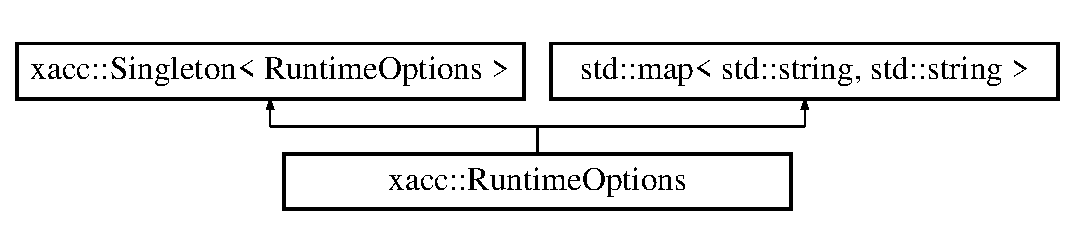
\includegraphics[height=12.000000cm]{a00060}
\end{center}
\end{figure}
\subsection*{Public Member Functions}
\begin{DoxyCompactItemize}
\item 
{\footnotesize template$<$typename HF , typename C\+NF , typename XF , typename YF , typename ZF , typename R\+XF , typename R\+YF , typename R\+ZF , typename MF , typename CF , typename C\+PF , typename S\+W\+A\+PF $>$ }\\{\bfseries Functional\+Gate\+Instruction\+Visitor} (HF h, C\+NF cn, XF x, YF y, ZF z, R\+XF rx, R\+YF ry, R\+ZF rz, MF m, CF c, C\+PF cp, S\+W\+A\+PF sw)\hypertarget{a00060_a4e3c27cd6b1acf063967b7b09a1eca09}{}\label{a00060_a4e3c27cd6b1acf063967b7b09a1eca09}

\item 
void {\bfseries visit} (\hyperlink{a00066}{Hadamard} \&h)\hypertarget{a00060_ac5245d34429dc112e7cd0e371108fcb5}{}\label{a00060_ac5245d34429dc112e7cd0e371108fcb5}

\item 
void {\bfseries visit} (\hyperlink{a00033}{C\+N\+OT} \&cn)\hypertarget{a00060_ad4eddafe8ca3906cd4aa5b98087a789a}{}\label{a00060_ad4eddafe8ca3906cd4aa5b98087a789a}

\item 
void {\bfseries visit} (\hyperlink{a00131}{X} \&x)\hypertarget{a00060_ac5d184daee7e755c9ede67b34bc2d091}{}\label{a00060_ac5d184daee7e755c9ede67b34bc2d091}

\item 
void {\bfseries visit} (\hyperlink{a00134}{Y} \&y)\hypertarget{a00060_a11dfa753a155346a45d7116a78c8f39f}{}\label{a00060_a11dfa753a155346a45d7116a78c8f39f}

\item 
void {\bfseries visit} (\hyperlink{a00135}{Z} \&z)\hypertarget{a00060_a4baf19da581fa9875739a227aba9cf60}{}\label{a00060_a4baf19da581fa9875739a227aba9cf60}

\item 
void {\bfseries visit} (\hyperlink{a00085}{Measure} \&m)\hypertarget{a00060_ad946faf8e2b6eff3e9e142907ec8e05a}{}\label{a00060_ad946faf8e2b6eff3e9e142907ec8e05a}

\item 
void {\bfseries visit} (\hyperlink{a00037}{Conditional\+Function} \&c)\hypertarget{a00060_a5cdb38902c241e7ae672a2631f1d61f3}{}\label{a00060_a5cdb38902c241e7ae672a2631f1d61f3}

\item 
void {\bfseries visit} (\hyperlink{a00114}{Rx} \&rx)\hypertarget{a00060_a6eb99e4b488773c750b7d9734ac1e885}{}\label{a00060_a6eb99e4b488773c750b7d9734ac1e885}

\item 
void {\bfseries visit} (\hyperlink{a00115}{Ry} \&ry)\hypertarget{a00060_aa22aad7b316386f5ef35672337c05ffc}{}\label{a00060_aa22aad7b316386f5ef35672337c05ffc}

\item 
void {\bfseries visit} (\hyperlink{a00040}{C\+Phase} \&cp)\hypertarget{a00060_a5475eece7afe380512a1a0215b92d302}{}\label{a00060_a5475eece7afe380512a1a0215b92d302}

\item 
void {\bfseries visit} (\hyperlink{a00116}{Rz} \&rz)\hypertarget{a00060_a8857ecf8f8f1b6143da8f31a722fe03e}{}\label{a00060_a8857ecf8f8f1b6143da8f31a722fe03e}

\item 
void {\bfseries visit} (\hyperlink{a00061}{Gate\+Function} \&f)\hypertarget{a00060_ad7d15225cf258fe59660ba828baff357}{}\label{a00060_ad7d15225cf258fe59660ba828baff357}

\item 
void {\bfseries visit} (\hyperlink{a00126}{Swap} \&s)\hypertarget{a00060_a30f46be43607813996c9cc090c1a5a16}{}\label{a00060_a30f46be43607813996c9cc090c1a5a16}

\end{DoxyCompactItemize}
\subsection*{Protected Attributes}
\begin{DoxyCompactItemize}
\item 
std\+::function$<$ void(\hyperlink{a00066}{Hadamard} \&)$>$ {\bfseries h\+Action}\hypertarget{a00060_a02f1401c9b0d1da801027f3bc0b5227e}{}\label{a00060_a02f1401c9b0d1da801027f3bc0b5227e}

\item 
std\+::function$<$ void(\hyperlink{a00033}{C\+N\+OT} \&)$>$ {\bfseries cnot\+Action}\hypertarget{a00060_a4d6bd8c2fd1af775ed08946942f60a0b}{}\label{a00060_a4d6bd8c2fd1af775ed08946942f60a0b}

\item 
std\+::function$<$ void(\hyperlink{a00131}{X} \&)$>$ {\bfseries x\+Action}\hypertarget{a00060_a9e0295434a2224b776609b057147a9af}{}\label{a00060_a9e0295434a2224b776609b057147a9af}

\item 
std\+::function$<$ void(\hyperlink{a00134}{Y} \&)$>$ {\bfseries y\+Action}\hypertarget{a00060_ae78f91a5cc9a7006f6bb1acee1c00501}{}\label{a00060_ae78f91a5cc9a7006f6bb1acee1c00501}

\item 
std\+::function$<$ void(\hyperlink{a00135}{Z} \&)$>$ {\bfseries z\+Action}\hypertarget{a00060_ae197f358e3d0777feb3656455e2ee672}{}\label{a00060_ae197f358e3d0777feb3656455e2ee672}

\item 
std\+::function$<$ void(\hyperlink{a00085}{Measure} \&)$>$ {\bfseries measure\+Action}\hypertarget{a00060_a239748abedd67c7b30cad12e545d1926}{}\label{a00060_a239748abedd67c7b30cad12e545d1926}

\item 
std\+::function$<$ void(\hyperlink{a00037}{Conditional\+Function} \&)$>$ {\bfseries cond\+Action}\hypertarget{a00060_a5c0595a70b1f7ae50f3e29a985e249e9}{}\label{a00060_a5c0595a70b1f7ae50f3e29a985e249e9}

\item 
std\+::function$<$ void(\hyperlink{a00114}{Rx} \&)$>$ {\bfseries rx\+Action}\hypertarget{a00060_ab79bb3eb3050d1c599061863bb2e219e}{}\label{a00060_ab79bb3eb3050d1c599061863bb2e219e}

\item 
std\+::function$<$ void(\hyperlink{a00115}{Ry} \&)$>$ {\bfseries ry\+Action}\hypertarget{a00060_a229b7d9aae52638c6eff04bd16bb9973}{}\label{a00060_a229b7d9aae52638c6eff04bd16bb9973}

\item 
std\+::function$<$ void(\hyperlink{a00116}{Rz} \&)$>$ {\bfseries rz\+Action}\hypertarget{a00060_a586ab5721150c67ad3ced46e2a236b44}{}\label{a00060_a586ab5721150c67ad3ced46e2a236b44}

\item 
std\+::function$<$ void(\hyperlink{a00040}{C\+Phase} \&)$>$ {\bfseries cp\+Action}\hypertarget{a00060_a5b88a0c9789e7b6d44527b2df6819ac5}{}\label{a00060_a5b88a0c9789e7b6d44527b2df6819ac5}

\item 
std\+::function$<$ void(\hyperlink{a00126}{Swap} \&)$>$ {\bfseries sw\+Action}\hypertarget{a00060_a5060cd4c2b1b259e32bda0e7ecc78e85}{}\label{a00060_a5060cd4c2b1b259e32bda0e7ecc78e85}

\end{DoxyCompactItemize}


The documentation for this class was generated from the following file\+:\begin{DoxyCompactItemize}
\item 
Functional\+Gate\+Instruction\+Visitor.\+hpp\end{DoxyCompactItemize}

\hypertarget{a00061}{}\section{xacc\+:\+:quantum\+:\+:Q\+FT Class Reference}
\label{a00061}\index{xacc\+::quantum\+::\+Q\+FT@{xacc\+::quantum\+::\+Q\+FT}}


{\ttfamily \#include $<$Q\+F\+T.\+hpp$>$}

Inheritance diagram for xacc\+:\+:quantum\+:\+:Q\+FT\+:\begin{figure}[H]
\begin{center}
\leavevmode
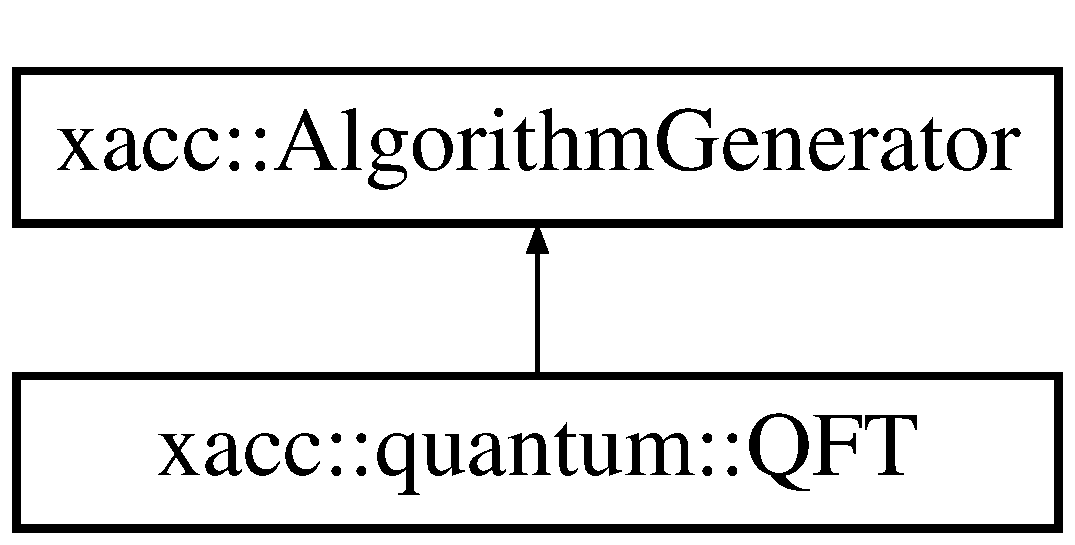
\includegraphics[height=2.000000cm]{a00061}
\end{center}
\end{figure}
\subsection*{Public Member Functions}
\begin{DoxyCompactItemize}
\item 
virtual std\+::shared\+\_\+ptr$<$ \hyperlink{a00039}{Function} $>$ \hyperlink{a00061_ac093c288bc9fc069464fc3fd2cc0ac21}{generate\+Algorithm} (std\+::vector$<$ int $>$ qubits)
\item 
virtual \hyperlink{a00061_a2f585738386f9a3744498983cd1f094e}{$\sim$\+Q\+FT} ()
\end{DoxyCompactItemize}


\subsection{Detailed Description}
\hyperlink{a00061}{Q\+FT} is a realization of the \hyperlink{a00014}{Algorithm\+Generator} interface that produces an X\+A\+CC \hyperlink{a00051}{IR} representation of the Quantum Fourier Transform.

\begin{DoxyAuthor}{Author}
Alex Mc\+Caskey 
\end{DoxyAuthor}


\subsection{Constructor \& Destructor Documentation}
\index{xacc\+::quantum\+::\+Q\+FT@{xacc\+::quantum\+::\+Q\+FT}!````~Q\+FT@{$\sim$\+Q\+FT}}
\index{````~Q\+FT@{$\sim$\+Q\+FT}!xacc\+::quantum\+::\+Q\+FT@{xacc\+::quantum\+::\+Q\+FT}}
\subsubsection[{\texorpdfstring{$\sim$\+Q\+F\+T()}{~QFT()}}]{\setlength{\rightskip}{0pt plus 5cm}virtual xacc\+::quantum\+::\+Q\+F\+T\+::$\sim$\+Q\+FT (
\begin{DoxyParamCaption}
{}
\end{DoxyParamCaption}
)\hspace{0.3cm}{\ttfamily [inline]}, {\ttfamily [virtual]}}\hypertarget{a00061_a2f585738386f9a3744498983cd1f094e}{}\label{a00061_a2f585738386f9a3744498983cd1f094e}
The destructor 

\subsection{Member Function Documentation}
\index{xacc\+::quantum\+::\+Q\+FT@{xacc\+::quantum\+::\+Q\+FT}!generate\+Algorithm@{generate\+Algorithm}}
\index{generate\+Algorithm@{generate\+Algorithm}!xacc\+::quantum\+::\+Q\+FT@{xacc\+::quantum\+::\+Q\+FT}}
\subsubsection[{\texorpdfstring{generate\+Algorithm(std\+::vector$<$ int $>$ qubits)}{generateAlgorithm(std::vector< int > qubits)}}]{\setlength{\rightskip}{0pt plus 5cm}std\+::shared\+\_\+ptr$<$ {\bf Function} $>$ xacc\+::quantum\+::\+Q\+F\+T\+::generate\+Algorithm (
\begin{DoxyParamCaption}
\item[{std\+::vector$<$ int $>$}]{qubits}
\end{DoxyParamCaption}
)\hspace{0.3cm}{\ttfamily [virtual]}}\hypertarget{a00061_ac093c288bc9fc069464fc3fd2cc0ac21}{}\label{a00061_ac093c288bc9fc069464fc3fd2cc0ac21}
This implementation returns a \hyperlink{a00039}{Function} \hyperlink{a00051}{IR} representation of the quantum fourier transform.


\begin{DoxyParams}{Parameters}
{\em bits} & The bits this algorithm operates on \\
\hline
\end{DoxyParams}
\begin{DoxyReturn}{Returns}
function The algorithm represented as an \hyperlink{a00051}{IR} \hyperlink{a00039}{Function} 
\end{DoxyReturn}


Implements \hyperlink{a00014_a73023c06f0f0c62ad56ab4187b18b096}{xacc\+::\+Algorithm\+Generator}.



The documentation for this class was generated from the following files\+:\begin{DoxyCompactItemize}
\item 
Q\+F\+T.\+hpp\item 
Q\+F\+T.\+cpp\end{DoxyCompactItemize}

\hypertarget{a00062}{}\section{xacc\+:\+:quantum\+:\+:Quantum\+Circuit Class Reference}
\label{a00062}\index{xacc\+::quantum\+::\+Quantum\+Circuit@{xacc\+::quantum\+::\+Quantum\+Circuit}}


{\ttfamily \#include $<$Quantum\+Circuit.\+hpp$>$}

Inheritance diagram for xacc\+:\+:quantum\+:\+:Quantum\+Circuit\+:\begin{figure}[H]
\begin{center}
\leavevmode
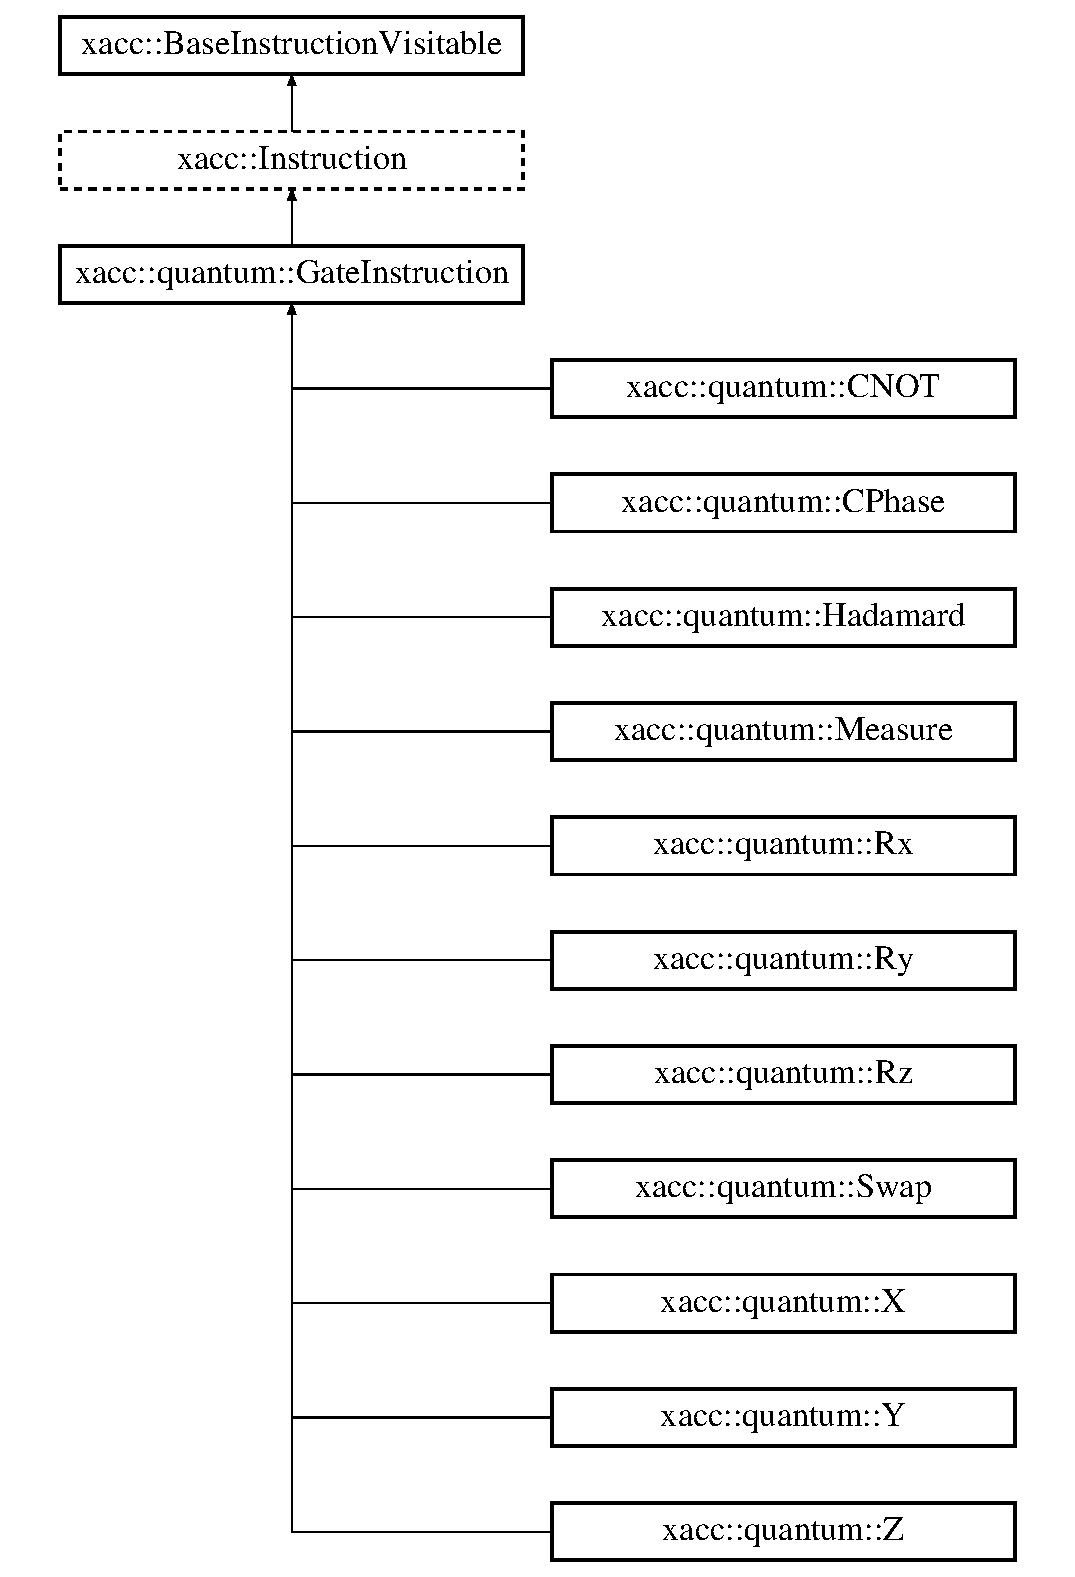
\includegraphics[height=2.000000cm]{a00062}
\end{center}
\end{figure}
\subsection*{Public Member Functions}
\begin{DoxyCompactItemize}
\item 
virtual void \hyperlink{a00062_af7a7f4a487d493fe8a4ed1f76cefd731}{read} (std\+::istream \&stream)
\end{DoxyCompactItemize}
\subsection*{Additional Inherited Members}


\subsection{Detailed Description}
The \hyperlink{a00062}{Quantum\+Circuit} is a subclass of \hyperlink{a00044}{Graph} that provides its Vertex template parameter as a \hyperlink{a00020}{Circuit\+Node}. It adds the ability to read Quantum\+Circuits from a graphviz dot file. 

\subsection{Member Function Documentation}
\index{xacc\+::quantum\+::\+Quantum\+Circuit@{xacc\+::quantum\+::\+Quantum\+Circuit}!read@{read}}
\index{read@{read}!xacc\+::quantum\+::\+Quantum\+Circuit@{xacc\+::quantum\+::\+Quantum\+Circuit}}
\subsubsection[{\texorpdfstring{read(std\+::istream \&stream)}{read(std::istream \&stream)}}]{\setlength{\rightskip}{0pt plus 5cm}virtual void xacc\+::quantum\+::\+Quantum\+Circuit\+::read (
\begin{DoxyParamCaption}
\item[{std\+::istream \&}]{stream}
\end{DoxyParamCaption}
)\hspace{0.3cm}{\ttfamily [inline]}, {\ttfamily [virtual]}}\hypertarget{a00062_af7a7f4a487d493fe8a4ed1f76cefd731}{}\label{a00062_af7a7f4a487d493fe8a4ed1f76cefd731}
Read in a graphviz dot graph from the given input stream. This is left for subclasses.


\begin{DoxyParams}{Parameters}
{\em stream} & \\
\hline
\end{DoxyParams}


Reimplemented from \hyperlink{a00044_abdd3e67dc08c223821d809bc8914164a}{xacc\+::\+Graph$<$ Circuit\+Node $>$}.



The documentation for this class was generated from the following file\+:\begin{DoxyCompactItemize}
\item 
Quantum\+Circuit.\+hpp\end{DoxyCompactItemize}

\hypertarget{a00063}{}\section{xacc\+:\+:quantum\+:\+:Quil\+Compiler Class Reference}
\label{a00063}\index{xacc\+::quantum\+::\+Quil\+Compiler@{xacc\+::quantum\+::\+Quil\+Compiler}}
Inheritance diagram for xacc\+:\+:quantum\+:\+:Quil\+Compiler\+:\begin{figure}[H]
\begin{center}
\leavevmode
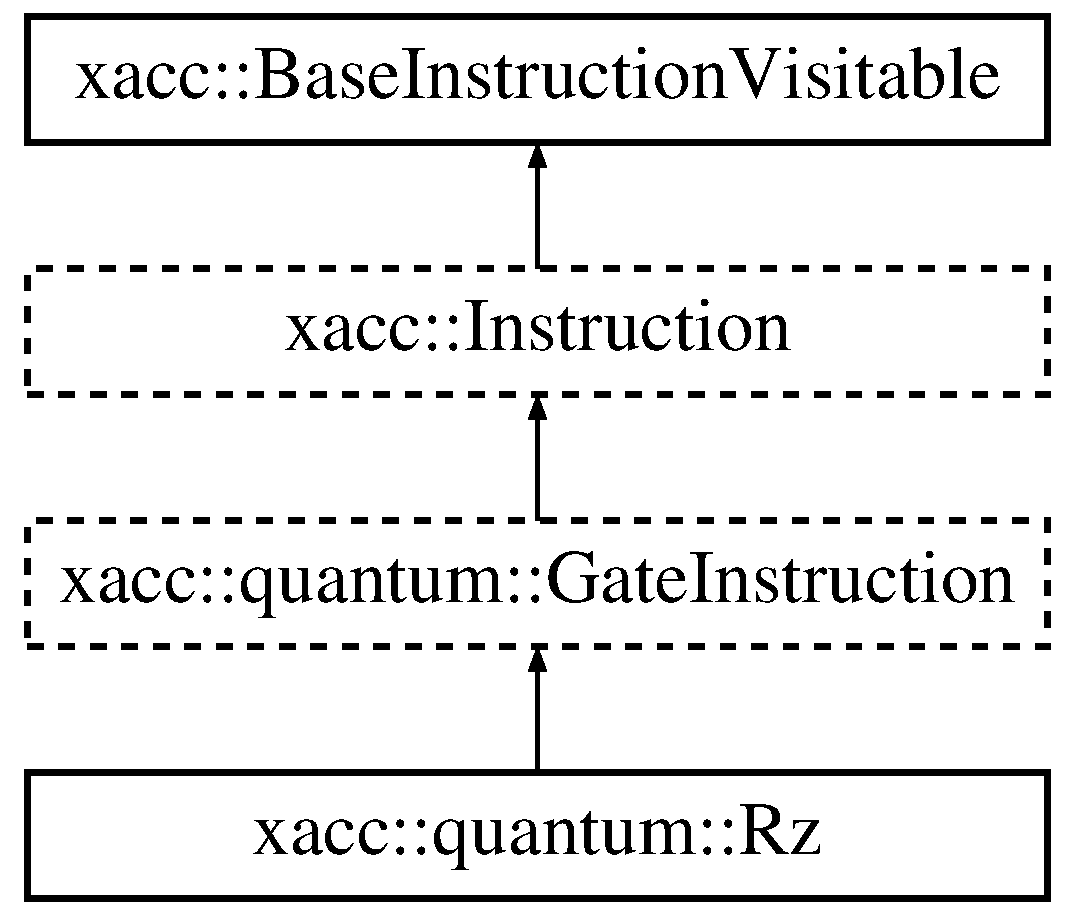
\includegraphics[height=3.000000cm]{a00063}
\end{center}
\end{figure}
\subsection*{Public Member Functions}
\begin{DoxyCompactItemize}
\item 
virtual std\+::shared\+\_\+ptr$<$ \hyperlink{a00051}{xacc\+::\+IR} $>$ \hyperlink{a00063_a2421482415ca4e09963ea4ecddff8100}{compile} (const std\+::string \&src, std\+::shared\+\_\+ptr$<$ \hyperlink{a00011}{Accelerator} $>$ acc)
\item 
virtual std\+::shared\+\_\+ptr$<$ \hyperlink{a00051}{xacc\+::\+IR} $>$ \hyperlink{a00063_adf4d321ecb0df3fa7728999f941c83b2}{compile} (const std\+::string \&src)
\item 
virtual const std\+::string \hyperlink{a00063_ae7d52140b6dd52730edc6e38ae48f437}{get\+Name} ()
\item 
virtual const std\+::string \hyperlink{a00063_a66ca00bbb1f30e7bc6dd86b1e267b93b}{translate} (const std\+::string \&buffer\+Variable, std\+::shared\+\_\+ptr$<$ \hyperlink{a00039}{Function} $>$ function)
\item 
virtual \hyperlink{a00063_a0866a9f695f28c90ac1f4754374f3bfe}{$\sim$\+Quil\+Compiler} ()
\end{DoxyCompactItemize}
\subsection*{Static Public Member Functions}
\begin{DoxyCompactItemize}
\item 
static void \hyperlink{a00063_aaec99a14bede717bf02a0f65af2a3c69}{register\+Compiler} ()
\end{DoxyCompactItemize}
\subsection*{Additional Inherited Members}


\subsection{Constructor \& Destructor Documentation}
\index{xacc\+::quantum\+::\+Quil\+Compiler@{xacc\+::quantum\+::\+Quil\+Compiler}!````~Quil\+Compiler@{$\sim$\+Quil\+Compiler}}
\index{````~Quil\+Compiler@{$\sim$\+Quil\+Compiler}!xacc\+::quantum\+::\+Quil\+Compiler@{xacc\+::quantum\+::\+Quil\+Compiler}}
\subsubsection[{\texorpdfstring{$\sim$\+Quil\+Compiler()}{~QuilCompiler()}}]{\setlength{\rightskip}{0pt plus 5cm}virtual xacc\+::quantum\+::\+Quil\+Compiler\+::$\sim$\+Quil\+Compiler (
\begin{DoxyParamCaption}
{}
\end{DoxyParamCaption}
)\hspace{0.3cm}{\ttfamily [inline]}, {\ttfamily [virtual]}}\hypertarget{a00063_a0866a9f695f28c90ac1f4754374f3bfe}{}\label{a00063_a0866a9f695f28c90ac1f4754374f3bfe}
The destructor 

\subsection{Member Function Documentation}
\index{xacc\+::quantum\+::\+Quil\+Compiler@{xacc\+::quantum\+::\+Quil\+Compiler}!compile@{compile}}
\index{compile@{compile}!xacc\+::quantum\+::\+Quil\+Compiler@{xacc\+::quantum\+::\+Quil\+Compiler}}
\subsubsection[{\texorpdfstring{compile(const std\+::string \&src, std\+::shared\+\_\+ptr$<$ Accelerator $>$ acc)}{compile(const std::string \&src, std::shared\_ptr< Accelerator > acc)}}]{\setlength{\rightskip}{0pt plus 5cm}std\+::shared\+\_\+ptr$<$ {\bf IR} $>$ xacc\+::quantum\+::\+Quil\+Compiler\+::compile (
\begin{DoxyParamCaption}
\item[{const std\+::string \&}]{src, }
\item[{std\+::shared\+\_\+ptr$<$ {\bf Accelerator} $>$}]{acc}
\end{DoxyParamCaption}
)\hspace{0.3cm}{\ttfamily [virtual]}}\hypertarget{a00063_a2421482415ca4e09963ea4ecddff8100}{}\label{a00063_a2421482415ca4e09963ea4ecddff8100}
Translate Quil to the X\+A\+CC intermediate representation.

\begin{DoxyReturn}{Returns}
ir X\+A\+CC intermediate representation 
\end{DoxyReturn}


Implements \hyperlink{a00023_a546a40c95bb93af6a0c0ac48dbeaffc8}{xacc\+::\+Compiler}.

\index{xacc\+::quantum\+::\+Quil\+Compiler@{xacc\+::quantum\+::\+Quil\+Compiler}!compile@{compile}}
\index{compile@{compile}!xacc\+::quantum\+::\+Quil\+Compiler@{xacc\+::quantum\+::\+Quil\+Compiler}}
\subsubsection[{\texorpdfstring{compile(const std\+::string \&src)}{compile(const std::string \&src)}}]{\setlength{\rightskip}{0pt plus 5cm}std\+::shared\+\_\+ptr$<$ {\bf IR} $>$ xacc\+::quantum\+::\+Quil\+Compiler\+::compile (
\begin{DoxyParamCaption}
\item[{const std\+::string \&}]{src}
\end{DoxyParamCaption}
)\hspace{0.3cm}{\ttfamily [virtual]}}\hypertarget{a00063_adf4d321ecb0df3fa7728999f941c83b2}{}\label{a00063_adf4d321ecb0df3fa7728999f941c83b2}

\begin{DoxyParams}{Parameters}
{\em src} & \\
\hline
\end{DoxyParams}
\begin{DoxyReturn}{Returns}

\end{DoxyReturn}


Implements \hyperlink{a00023_a9092f5f779b570c91569b59621280c04}{xacc\+::\+Compiler}.

\index{xacc\+::quantum\+::\+Quil\+Compiler@{xacc\+::quantum\+::\+Quil\+Compiler}!get\+Name@{get\+Name}}
\index{get\+Name@{get\+Name}!xacc\+::quantum\+::\+Quil\+Compiler@{xacc\+::quantum\+::\+Quil\+Compiler}}
\subsubsection[{\texorpdfstring{get\+Name()}{getName()}}]{\setlength{\rightskip}{0pt plus 5cm}virtual const std\+::string xacc\+::quantum\+::\+Quil\+Compiler\+::get\+Name (
\begin{DoxyParamCaption}
{}
\end{DoxyParamCaption}
)\hspace{0.3cm}{\ttfamily [inline]}, {\ttfamily [virtual]}}\hypertarget{a00063_ae7d52140b6dd52730edc6e38ae48f437}{}\label{a00063_ae7d52140b6dd52730edc6e38ae48f437}
Return the name of this \hyperlink{a00023}{Compiler} \begin{DoxyReturn}{Returns}
name \hyperlink{a00023}{Compiler} name 
\end{DoxyReturn}


Implements \hyperlink{a00023_a87fca9100e6462122f5b687c3a0fb3fb}{xacc\+::\+Compiler}.

\index{xacc\+::quantum\+::\+Quil\+Compiler@{xacc\+::quantum\+::\+Quil\+Compiler}!register\+Compiler@{register\+Compiler}}
\index{register\+Compiler@{register\+Compiler}!xacc\+::quantum\+::\+Quil\+Compiler@{xacc\+::quantum\+::\+Quil\+Compiler}}
\subsubsection[{\texorpdfstring{register\+Compiler()}{registerCompiler()}}]{\setlength{\rightskip}{0pt plus 5cm}static void xacc\+::quantum\+::\+Quil\+Compiler\+::register\+Compiler (
\begin{DoxyParamCaption}
{}
\end{DoxyParamCaption}
)\hspace{0.3cm}{\ttfamily [inline]}, {\ttfamily [static]}}\hypertarget{a00063_aaec99a14bede717bf02a0f65af2a3c69}{}\label{a00063_aaec99a14bede717bf02a0f65af2a3c69}
Register this \hyperlink{a00023}{Compiler} with the framework. \index{xacc\+::quantum\+::\+Quil\+Compiler@{xacc\+::quantum\+::\+Quil\+Compiler}!translate@{translate}}
\index{translate@{translate}!xacc\+::quantum\+::\+Quil\+Compiler@{xacc\+::quantum\+::\+Quil\+Compiler}}
\subsubsection[{\texorpdfstring{translate(const std\+::string \&buffer\+Variable, std\+::shared\+\_\+ptr$<$ Function $>$ function)}{translate(const std::string \&bufferVariable, std::shared\_ptr< Function > function)}}]{\setlength{\rightskip}{0pt plus 5cm}const std\+::string xacc\+::quantum\+::\+Quil\+Compiler\+::translate (
\begin{DoxyParamCaption}
\item[{const std\+::string \&}]{buffer\+Variable, }
\item[{std\+::shared\+\_\+ptr$<$ {\bf Function} $>$}]{function}
\end{DoxyParamCaption}
)\hspace{0.3cm}{\ttfamily [virtual]}}\hypertarget{a00063_a66ca00bbb1f30e7bc6dd86b1e267b93b}{}\label{a00063_a66ca00bbb1f30e7bc6dd86b1e267b93b}
This produces a Quil source code representation of the given \hyperlink{a00051}{IR} \hyperlink{a00039}{Function}


\begin{DoxyParams}{Parameters}
{\em function} & The X\+A\+CC \hyperlink{a00051}{IR} \hyperlink{a00039}{Function} to translate \\
\hline
\end{DoxyParams}
\begin{DoxyReturn}{Returns}
src The source code as a string 
\end{DoxyReturn}


Implements \hyperlink{a00023_aeedbe58a33fed29e4d7694ae743e25e7}{xacc\+::\+Compiler}.



The documentation for this class was generated from the following files\+:\begin{DoxyCompactItemize}
\item 
Quil\+Compiler.\+hpp\item 
Quil\+Compiler.\+cpp\end{DoxyCompactItemize}

\hypertarget{a00064}{}\section{boost\+:\+:dll\+:\+:detail\+:\+:constructor$<$ Class(Args...)$>$ Struct Template Reference}
\label{a00064}\index{boost\+::dll\+::detail\+::constructor$<$ Class(\+Args...)$>$@{boost\+::dll\+::detail\+::constructor$<$ Class(\+Args...)$>$}}
\subsection*{Public Types}
\begin{DoxyCompactItemize}
\item 
typedef \hyperlink{a00131}{detail\+::get\+\_\+mem\+\_\+fn\+\_\+type}$<$ Class, void(Args...)$>$\+::mem\+\_\+fn {\bfseries standard\+\_\+t}\hypertarget{a00064_ab765d8c7c083efce92a933c806a41e81}{}\label{a00064_ab765d8c7c083efce92a933c806a41e81}

\item 
typedef Class $\ast$($\ast$ {\bfseries allocating\+\_\+t}) (Args...)\hypertarget{a00064_a19159ea77e5c102bd216195b32045677}{}\label{a00064_a19159ea77e5c102bd216195b32045677}

\end{DoxyCompactItemize}
\subsection*{Public Member Functions}
\begin{DoxyCompactItemize}
\item 
void \hyperlink{a00064_a2b0dbd4b6c5fb1c8fa284b64f85e3caa}{call\+\_\+standard} (Class $\ast$const ptr, Args...\+args)\hypertarget{a00064_a2b0dbd4b6c5fb1c8fa284b64f85e3caa}{}\label{a00064_a2b0dbd4b6c5fb1c8fa284b64f85e3caa}

\begin{DoxyCompactList}\small\item\em Call the standard contructor. \end{DoxyCompactList}\item 
Class $\ast$ \hyperlink{a00064_a9674344355e9759b8f60a4eb92e718af}{call\+\_\+allocating} (Args...\+args)\hypertarget{a00064_a9674344355e9759b8f60a4eb92e718af}{}\label{a00064_a9674344355e9759b8f60a4eb92e718af}

\begin{DoxyCompactList}\small\item\em Call the deleting destructor. \end{DoxyCompactList}\item 
bool \hyperlink{a00064_a2bb649c5d51e8ae9656db16b65776f1c}{has\+\_\+allocating} () const \hypertarget{a00064_a2bb649c5d51e8ae9656db16b65776f1c}{}\label{a00064_a2bb649c5d51e8ae9656db16b65776f1c}

\begin{DoxyCompactList}\small\item\em True if a allocating constructor could be loaded. \end{DoxyCompactList}\item 
bool \hyperlink{a00064_a383752514de8d2f1ffdd142f642e54a3}{has\+\_\+standard} () const \hypertarget{a00064_a383752514de8d2f1ffdd142f642e54a3}{}\label{a00064_a383752514de8d2f1ffdd142f642e54a3}

\begin{DoxyCompactList}\small\item\em True if a standard constructor could be loaded. \end{DoxyCompactList}\item 
bool \hyperlink{a00064_af65e82bd30161ccf3ea05f87193c3fa1}{is\+\_\+empty} () const \hypertarget{a00064_af65e82bd30161ccf3ea05f87193c3fa1}{}\label{a00064_af65e82bd30161ccf3ea05f87193c3fa1}

\begin{DoxyCompactList}\small\item\em False if neither the allocating nor the standard constructor is available. \end{DoxyCompactList}\item 
{\bfseries constructor} (const \hyperlink{a00063}{constructor} \&)=default\hypertarget{a00064_a6ae77617757558a1b0177d6a2cae9827}{}\label{a00064_a6ae77617757558a1b0177d6a2cae9827}

\item 
{\bfseries constructor} (standard\+\_\+t \hyperlink{a00064_a6cbccda8c81959e8e3bba7da28cada5d}{standard}, allocating\+\_\+t \hyperlink{a00064_a13c90a276dc453ca83da117ffc552362}{allocating}=nullptr)\hypertarget{a00064_a403d27f9f509c0ce4e66d4713ca2affc}{}\label{a00064_a403d27f9f509c0ce4e66d4713ca2affc}

\end{DoxyCompactItemize}
\subsection*{Public Attributes}
\begin{DoxyCompactItemize}
\item 
standard\+\_\+t \hyperlink{a00064_a6cbccda8c81959e8e3bba7da28cada5d}{standard}
\begin{DoxyCompactList}\small\item\em The standard, i.\+e. not allocating constructor. \end{DoxyCompactList}\item 
allocating\+\_\+t \hyperlink{a00064_a13c90a276dc453ca83da117ffc552362}{allocating}
\begin{DoxyCompactList}\small\item\em The allocating constructor. \end{DoxyCompactList}\end{DoxyCompactItemize}


\subsection{Member Data Documentation}
\index{boost\+::dll\+::detail\+::constructor$<$ Class(\+Args...)$>$@{boost\+::dll\+::detail\+::constructor$<$ Class(\+Args...)$>$}!allocating@{allocating}}
\index{allocating@{allocating}!boost\+::dll\+::detail\+::constructor$<$ Class(\+Args...)$>$@{boost\+::dll\+::detail\+::constructor$<$ Class(\+Args...)$>$}}
\subsubsection[{\texorpdfstring{allocating}{allocating}}]{\setlength{\rightskip}{0pt plus 5cm}template$<$typename Class , typename... Args$>$ allocating\+\_\+t {\bf boost\+::dll\+::detail\+::constructor}$<$ Class(Args...)$>$\+::allocating}\hypertarget{a00064_a13c90a276dc453ca83da117ffc552362}{}\label{a00064_a13c90a276dc453ca83da117ffc552362}


The allocating constructor. 

\begin{DoxyWarning}{Warning}
May differ with the compiler. Use constructor\+::call\+\_\+allocating instead. 
\end{DoxyWarning}
\index{boost\+::dll\+::detail\+::constructor$<$ Class(\+Args...)$>$@{boost\+::dll\+::detail\+::constructor$<$ Class(\+Args...)$>$}!standard@{standard}}
\index{standard@{standard}!boost\+::dll\+::detail\+::constructor$<$ Class(\+Args...)$>$@{boost\+::dll\+::detail\+::constructor$<$ Class(\+Args...)$>$}}
\subsubsection[{\texorpdfstring{standard}{standard}}]{\setlength{\rightskip}{0pt plus 5cm}template$<$typename Class , typename... Args$>$ standard\+\_\+t {\bf boost\+::dll\+::detail\+::constructor}$<$ Class(Args...)$>$\+::standard}\hypertarget{a00064_a6cbccda8c81959e8e3bba7da28cada5d}{}\label{a00064_a6cbccda8c81959e8e3bba7da28cada5d}


The standard, i.\+e. not allocating constructor. 

\begin{DoxyWarning}{Warning}
May differ with the compiler. Use constructor\+::call\+\_\+standard instead. 
\end{DoxyWarning}


The documentation for this struct was generated from the following file\+:\begin{DoxyCompactItemize}
\item 
ctor\+\_\+dtor.\+hpp\end{DoxyCompactItemize}

\hypertarget{a00065}{}\section{xacc\+:\+:Register\+Algorithm\+Generator$<$ T $>$ Class Template Reference}
\label{a00065}\index{xacc\+::\+Register\+Algorithm\+Generator$<$ T $>$@{xacc\+::\+Register\+Algorithm\+Generator$<$ T $>$}}


{\ttfamily \#include $<$Algorithm\+Generator.\+hpp$>$}

\subsection*{Public Member Functions}
\begin{DoxyCompactItemize}
\item 
{\bfseries Register\+Algorithm\+Generator} (const std\+::string \&name)\hypertarget{a00065_af439cc4d7c8d6628a979129a5c1411df}{}\label{a00065_af439cc4d7c8d6628a979129a5c1411df}

\end{DoxyCompactItemize}


\subsection{Detailed Description}
\subsubsection*{template$<$typename T$>$\\*
class xacc\+::\+Register\+Algorithm\+Generator$<$ T $>$}

\hyperlink{a00065}{Register\+Algorithm\+Generator} is a convenience class for registering custom derived \hyperlink{a00014}{Algorithm\+Generator} classes.

Creators of \hyperlink{a00014}{Algorithm\+Generator} subclasses create an instance of this class with their \hyperlink{a00014}{Algorithm\+Generator} subclass as the template parameter to register their \hyperlink{a00014}{Algorithm\+Generator} with X\+A\+CC. This instance must be created in the C\+PP implementation file for the \hyperlink{a00014}{Algorithm\+Generator} and at global scope. 

The documentation for this class was generated from the following file\+:\begin{DoxyCompactItemize}
\item 
Algorithm\+Generator.\+hpp\end{DoxyCompactItemize}

\hypertarget{a00066}{}\section{xacc\+:\+:Register\+Compiler$<$ T $>$ Class Template Reference}
\label{a00066}\index{xacc\+::\+Register\+Compiler$<$ T $>$@{xacc\+::\+Register\+Compiler$<$ T $>$}}


{\ttfamily \#include $<$Compiler.\+hpp$>$}

\subsection*{Public Member Functions}
\begin{DoxyCompactItemize}
\item 
{\bfseries Register\+Compiler} (const std\+::string \&name)\hypertarget{a00066_a41f5c1abd570b3867b9790cdc02f3355}{}\label{a00066_a41f5c1abd570b3867b9790cdc02f3355}

\item 
{\bfseries Register\+Compiler} (const std\+::string \&name, std\+::shared\+\_\+ptr$<$ options\+\_\+description $>$ options)\hypertarget{a00066_a3489e8cf59f2b0c14e4e2037b61bc368}{}\label{a00066_a3489e8cf59f2b0c14e4e2037b61bc368}

\end{DoxyCompactItemize}


\subsection{Detailed Description}
\subsubsection*{template$<$typename T$>$\\*
class xacc\+::\+Register\+Compiler$<$ T $>$}

\hyperlink{a00066}{Register\+Compiler} is a convenience class for registering custom derived \hyperlink{a00023}{Compiler} classes.

Creators of \hyperlink{a00023}{Compiler} subclasses create an instance of this class with their \hyperlink{a00023}{Compiler} subclass as the template parameter to register their \hyperlink{a00023}{Compiler} with X\+A\+CC. This instance must be created in the C\+PP implementation file for the \hyperlink{a00023}{Compiler} and at global scope. 

The documentation for this class was generated from the following file\+:\begin{DoxyCompactItemize}
\item 
Compiler.\+hpp\end{DoxyCompactItemize}

\hypertarget{a00067}{}\section{xacc\+:\+:quantum\+:\+:Simulated\+Qubits$<$ Total\+Number\+Of\+Qubits $>$ Class Template Reference}
\label{a00067}\index{xacc\+::quantum\+::\+Simulated\+Qubits$<$ Total\+Number\+Of\+Qubits $>$@{xacc\+::quantum\+::\+Simulated\+Qubits$<$ Total\+Number\+Of\+Qubits $>$}}


{\ttfamily \#include $<$Simulated\+Qubits.\+hpp$>$}

Inheritance diagram for xacc\+:\+:quantum\+:\+:Simulated\+Qubits$<$ Total\+Number\+Of\+Qubits $>$\+:\begin{figure}[H]
\begin{center}
\leavevmode
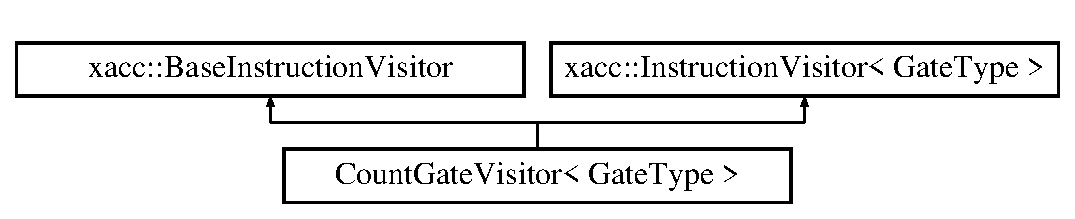
\includegraphics[height=2.000000cm]{a00067}
\end{center}
\end{figure}
\subsection*{Public Member Functions}
\begin{DoxyCompactItemize}
\item 
\hyperlink{a00067_afeb610fbd0c761caa15136e77260ba48}{Simulated\+Qubits} (const std\+::string \&str)
\item 
\hyperlink{a00067_a3d0f465d821565c582c37b6b4d7e4f79}{Simulated\+Qubits} (const std\+::string \&str, const int N)
\item 
{\footnotesize template$<$typename... Indices$>$ }\\{\bfseries Simulated\+Qubits} (const std\+::string \&str, int first\+Index, Indices...\+indices)\hypertarget{a00067_a9366eb77384fb1e9f34a693b9a7ea1b8}{}\label{a00067_a9366eb77384fb1e9f34a693b9a7ea1b8}

\item 
void \hyperlink{a00067_a97ecaaf5aab14bc017726fe9cfd41c46}{apply\+Unitary} (fire\+::\+Tensor$<$ 2, fire\+::\+Eigen\+Provider, std\+::complex$<$ double $>$$>$ \&U)
\item 
void \hyperlink{a00067_aea8a0358100e815a7c70eee7f8ba9d45}{normalize} ()
\item 
Qubit\+State \& \hyperlink{a00067_a75b8fde8e812931fe087cb078108c00d}{get\+State} ()
\item 
void \hyperlink{a00067_a2a0e202f943d3ec8d848c7e25062c6e1}{set\+State} (Qubit\+State \&st)
\item 
virtual bool \hyperlink{a00067_ac689b60b0218bf8d0c11ef2f151e7272}{is\+Valid\+Buffer\+Size} (const int N)
\item 
virtual void \hyperlink{a00067_ad9a39b44161fa0309167b9791ed10945}{print} (std\+::ostream \&stream)
\item 
virtual void {\bfseries print} ()\hypertarget{a00067_a7cda9427b5a0d3eaa9573eb9d992f51c}{}\label{a00067_a7cda9427b5a0d3eaa9573eb9d992f51c}

\end{DoxyCompactItemize}
\subsection*{Protected Attributes}
\begin{DoxyCompactItemize}
\item 
Qubit\+State \hyperlink{a00067_ade9f334823890b3c0553800188ac3ef9}{buffer\+State}
\end{DoxyCompactItemize}


\subsection{Detailed Description}
\subsubsection*{template$<$const int Total\+Number\+Of\+Qubits$>$\\*
class xacc\+::quantum\+::\+Simulated\+Qubits$<$ Total\+Number\+Of\+Qubits $>$}

\hyperlink{a00067}{Simulated\+Qubits} is an \hyperlink{a00013}{Accelerator\+Buffer} that models simulated qubits. As such, it keeps track of the state of the qubit buffer using a Rank 1 Fire Tensor.

It provides an interface for applying unitary operations on the qubit buffer state. 

\subsection{Constructor \& Destructor Documentation}
\index{xacc\+::quantum\+::\+Simulated\+Qubits@{xacc\+::quantum\+::\+Simulated\+Qubits}!Simulated\+Qubits@{Simulated\+Qubits}}
\index{Simulated\+Qubits@{Simulated\+Qubits}!xacc\+::quantum\+::\+Simulated\+Qubits@{xacc\+::quantum\+::\+Simulated\+Qubits}}
\subsubsection[{\texorpdfstring{Simulated\+Qubits(const std\+::string \&str)}{SimulatedQubits(const std::string \&str)}}]{\setlength{\rightskip}{0pt plus 5cm}template$<$const int Total\+Number\+Of\+Qubits$>$ {\bf xacc\+::quantum\+::\+Simulated\+Qubits}$<$ Total\+Number\+Of\+Qubits $>$\+::{\bf Simulated\+Qubits} (
\begin{DoxyParamCaption}
\item[{const std\+::string \&}]{str}
\end{DoxyParamCaption}
)\hspace{0.3cm}{\ttfamily [inline]}}\hypertarget{a00067_afeb610fbd0c761caa15136e77260ba48}{}\label{a00067_afeb610fbd0c761caa15136e77260ba48}
The Constructor, creates a state of size 2$^\wedge$\+Total\+Number\+Of\+Qubits.


\begin{DoxyParams}{Parameters}
{\em str} & \\
\hline
\end{DoxyParams}
\index{xacc\+::quantum\+::\+Simulated\+Qubits@{xacc\+::quantum\+::\+Simulated\+Qubits}!Simulated\+Qubits@{Simulated\+Qubits}}
\index{Simulated\+Qubits@{Simulated\+Qubits}!xacc\+::quantum\+::\+Simulated\+Qubits@{xacc\+::quantum\+::\+Simulated\+Qubits}}
\subsubsection[{\texorpdfstring{Simulated\+Qubits(const std\+::string \&str, const int N)}{SimulatedQubits(const std::string \&str, const int N)}}]{\setlength{\rightskip}{0pt plus 5cm}template$<$const int Total\+Number\+Of\+Qubits$>$ {\bf xacc\+::quantum\+::\+Simulated\+Qubits}$<$ Total\+Number\+Of\+Qubits $>$\+::{\bf Simulated\+Qubits} (
\begin{DoxyParamCaption}
\item[{const std\+::string \&}]{str, }
\item[{const int}]{N}
\end{DoxyParamCaption}
)\hspace{0.3cm}{\ttfamily [inline]}}\hypertarget{a00067_a3d0f465d821565c582c37b6b4d7e4f79}{}\label{a00067_a3d0f465d821565c582c37b6b4d7e4f79}
The Constructor, creates a state with given size N. 
\begin{DoxyParams}{Parameters}
{\em str} & \\
\hline
{\em N} & \\
\hline
\end{DoxyParams}


\subsection{Member Function Documentation}
\index{xacc\+::quantum\+::\+Simulated\+Qubits@{xacc\+::quantum\+::\+Simulated\+Qubits}!apply\+Unitary@{apply\+Unitary}}
\index{apply\+Unitary@{apply\+Unitary}!xacc\+::quantum\+::\+Simulated\+Qubits@{xacc\+::quantum\+::\+Simulated\+Qubits}}
\subsubsection[{\texorpdfstring{apply\+Unitary(fire\+::\+Tensor$<$ 2, fire\+::\+Eigen\+Provider, std\+::complex$<$ double $>$$>$ \&\+U)}{applyUnitary(fire::Tensor< 2, fire::EigenProvider, std::complex< double >> \&U)}}]{\setlength{\rightskip}{0pt plus 5cm}template$<$const int Total\+Number\+Of\+Qubits$>$ void {\bf xacc\+::quantum\+::\+Simulated\+Qubits}$<$ Total\+Number\+Of\+Qubits $>$\+::apply\+Unitary (
\begin{DoxyParamCaption}
\item[{fire\+::\+Tensor$<$ 2, fire\+::\+Eigen\+Provider, std\+::complex$<$ double $>$$>$ \&}]{U}
\end{DoxyParamCaption}
)\hspace{0.3cm}{\ttfamily [inline]}}\hypertarget{a00067_a97ecaaf5aab14bc017726fe9cfd41c46}{}\label{a00067_a97ecaaf5aab14bc017726fe9cfd41c46}
Apply the given unitary matrix to this qubit buffer state.


\begin{DoxyParams}{Parameters}
{\em U} & \\
\hline
\end{DoxyParams}
\index{xacc\+::quantum\+::\+Simulated\+Qubits@{xacc\+::quantum\+::\+Simulated\+Qubits}!get\+State@{get\+State}}
\index{get\+State@{get\+State}!xacc\+::quantum\+::\+Simulated\+Qubits@{xacc\+::quantum\+::\+Simulated\+Qubits}}
\subsubsection[{\texorpdfstring{get\+State()}{getState()}}]{\setlength{\rightskip}{0pt plus 5cm}template$<$const int Total\+Number\+Of\+Qubits$>$ Qubit\+State\& {\bf xacc\+::quantum\+::\+Simulated\+Qubits}$<$ Total\+Number\+Of\+Qubits $>$\+::get\+State (
\begin{DoxyParamCaption}
{}
\end{DoxyParamCaption}
)\hspace{0.3cm}{\ttfamily [inline]}}\hypertarget{a00067_a75b8fde8e812931fe087cb078108c00d}{}\label{a00067_a75b8fde8e812931fe087cb078108c00d}
Return the current state

\begin{DoxyReturn}{Returns}

\end{DoxyReturn}
\index{xacc\+::quantum\+::\+Simulated\+Qubits@{xacc\+::quantum\+::\+Simulated\+Qubits}!is\+Valid\+Buffer\+Size@{is\+Valid\+Buffer\+Size}}
\index{is\+Valid\+Buffer\+Size@{is\+Valid\+Buffer\+Size}!xacc\+::quantum\+::\+Simulated\+Qubits@{xacc\+::quantum\+::\+Simulated\+Qubits}}
\subsubsection[{\texorpdfstring{is\+Valid\+Buffer\+Size(const int N)}{isValidBufferSize(const int N)}}]{\setlength{\rightskip}{0pt plus 5cm}template$<$const int Total\+Number\+Of\+Qubits$>$ virtual bool {\bf xacc\+::quantum\+::\+Simulated\+Qubits}$<$ Total\+Number\+Of\+Qubits $>$\+::is\+Valid\+Buffer\+Size (
\begin{DoxyParamCaption}
\item[{const int}]{N}
\end{DoxyParamCaption}
)\hspace{0.3cm}{\ttfamily [inline]}, {\ttfamily [virtual]}}\hypertarget{a00067_ac689b60b0218bf8d0c11ef2f151e7272}{}\label{a00067_ac689b60b0218bf8d0c11ef2f151e7272}
Allocating this buffer type is only valid if N $<$= Total\+Number\+Of\+Qubits. 
\begin{DoxyParams}{Parameters}
{\em N} & \\
\hline
\end{DoxyParams}
\begin{DoxyReturn}{Returns}

\end{DoxyReturn}
\index{xacc\+::quantum\+::\+Simulated\+Qubits@{xacc\+::quantum\+::\+Simulated\+Qubits}!normalize@{normalize}}
\index{normalize@{normalize}!xacc\+::quantum\+::\+Simulated\+Qubits@{xacc\+::quantum\+::\+Simulated\+Qubits}}
\subsubsection[{\texorpdfstring{normalize()}{normalize()}}]{\setlength{\rightskip}{0pt plus 5cm}template$<$const int Total\+Number\+Of\+Qubits$>$ void {\bf xacc\+::quantum\+::\+Simulated\+Qubits}$<$ Total\+Number\+Of\+Qubits $>$\+::normalize (
\begin{DoxyParamCaption}
{}
\end{DoxyParamCaption}
)\hspace{0.3cm}{\ttfamily [inline]}}\hypertarget{a00067_aea8a0358100e815a7c70eee7f8ba9d45}{}\label{a00067_aea8a0358100e815a7c70eee7f8ba9d45}
Normalize the state. \index{xacc\+::quantum\+::\+Simulated\+Qubits@{xacc\+::quantum\+::\+Simulated\+Qubits}!print@{print}}
\index{print@{print}!xacc\+::quantum\+::\+Simulated\+Qubits@{xacc\+::quantum\+::\+Simulated\+Qubits}}
\subsubsection[{\texorpdfstring{print(std\+::ostream \&stream)}{print(std::ostream \&stream)}}]{\setlength{\rightskip}{0pt plus 5cm}template$<$const int Total\+Number\+Of\+Qubits$>$ virtual void {\bf xacc\+::quantum\+::\+Simulated\+Qubits}$<$ Total\+Number\+Of\+Qubits $>$\+::print (
\begin{DoxyParamCaption}
\item[{std\+::ostream \&}]{stream}
\end{DoxyParamCaption}
)\hspace{0.3cm}{\ttfamily [inline]}, {\ttfamily [virtual]}}\hypertarget{a00067_ad9a39b44161fa0309167b9791ed10945}{}\label{a00067_ad9a39b44161fa0309167b9791ed10945}
Print the state to the provided output stream.


\begin{DoxyParams}{Parameters}
{\em stream} & \\
\hline
\end{DoxyParams}


Reimplemented from \hyperlink{a00013}{Accelerator\+Buffer}.

\index{xacc\+::quantum\+::\+Simulated\+Qubits@{xacc\+::quantum\+::\+Simulated\+Qubits}!set\+State@{set\+State}}
\index{set\+State@{set\+State}!xacc\+::quantum\+::\+Simulated\+Qubits@{xacc\+::quantum\+::\+Simulated\+Qubits}}
\subsubsection[{\texorpdfstring{set\+State(\+Qubit\+State \&st)}{setState(QubitState \&st)}}]{\setlength{\rightskip}{0pt plus 5cm}template$<$const int Total\+Number\+Of\+Qubits$>$ void {\bf xacc\+::quantum\+::\+Simulated\+Qubits}$<$ Total\+Number\+Of\+Qubits $>$\+::set\+State (
\begin{DoxyParamCaption}
\item[{Qubit\+State \&}]{st}
\end{DoxyParamCaption}
)\hspace{0.3cm}{\ttfamily [inline]}}\hypertarget{a00067_a2a0e202f943d3ec8d848c7e25062c6e1}{}\label{a00067_a2a0e202f943d3ec8d848c7e25062c6e1}
Set the state. 
\begin{DoxyParams}{Parameters}
{\em st} & \\
\hline
\end{DoxyParams}


\subsection{Member Data Documentation}
\index{xacc\+::quantum\+::\+Simulated\+Qubits@{xacc\+::quantum\+::\+Simulated\+Qubits}!buffer\+State@{buffer\+State}}
\index{buffer\+State@{buffer\+State}!xacc\+::quantum\+::\+Simulated\+Qubits@{xacc\+::quantum\+::\+Simulated\+Qubits}}
\subsubsection[{\texorpdfstring{buffer\+State}{bufferState}}]{\setlength{\rightskip}{0pt plus 5cm}template$<$const int Total\+Number\+Of\+Qubits$>$ Qubit\+State {\bf xacc\+::quantum\+::\+Simulated\+Qubits}$<$ Total\+Number\+Of\+Qubits $>$\+::buffer\+State\hspace{0.3cm}{\ttfamily [protected]}}\hypertarget{a00067_ade9f334823890b3c0553800188ac3ef9}{}\label{a00067_ade9f334823890b3c0553800188ac3ef9}
The qubit buffer state. 

The documentation for this class was generated from the following file\+:\begin{DoxyCompactItemize}
\item 
Simulated\+Qubits.\+hpp\end{DoxyCompactItemize}

\hypertarget{a00068}{}\section{Crt\+Allocator Class Reference}
\label{a00068}\index{Crt\+Allocator@{Crt\+Allocator}}


C-\/runtime library allocator.  




{\ttfamily \#include $<$allocators.\+h$>$}

\subsection*{Public Member Functions}
\begin{DoxyCompactItemize}
\item 
void $\ast$ {\bfseries Malloc} (size\+\_\+t size)\hypertarget{a00068_acd720631f8c094041afa6c7951f0d935}{}\label{a00068_acd720631f8c094041afa6c7951f0d935}

\item 
void $\ast$ {\bfseries Realloc} (void $\ast$original\+Ptr, size\+\_\+t original\+Size, size\+\_\+t new\+Size)\hypertarget{a00068_a646bb6f68afe773a62a22f7f14f83e97}{}\label{a00068_a646bb6f68afe773a62a22f7f14f83e97}

\end{DoxyCompactItemize}
\subsection*{Static Public Member Functions}
\begin{DoxyCompactItemize}
\item 
static void {\bfseries Free} (void $\ast$ptr)\hypertarget{a00068_a5043907058d906dcb1291e9491560373}{}\label{a00068_a5043907058d906dcb1291e9491560373}

\end{DoxyCompactItemize}
\subsection*{Static Public Attributes}
\begin{DoxyCompactItemize}
\item 
static const bool {\bfseries k\+Need\+Free} = true\hypertarget{a00068_ac7df8398c529290f0cd5950d9492f524}{}\label{a00068_ac7df8398c529290f0cd5950d9492f524}

\end{DoxyCompactItemize}


\subsection{Detailed Description}
C-\/runtime library allocator. 

This class is just wrapper for standard C library memory routines. \begin{DoxyNote}{Note}
implements Allocator concept 
\end{DoxyNote}


The documentation for this class was generated from the following file\+:\begin{DoxyCompactItemize}
\item 
allocators.\+h\end{DoxyCompactItemize}

\hypertarget{a00069}{}\section{xacc\+:\+:Register\+Preprocessor$<$ T $>$ Class Template Reference}
\label{a00069}\index{xacc\+::\+Register\+Preprocessor$<$ T $>$@{xacc\+::\+Register\+Preprocessor$<$ T $>$}}


{\ttfamily \#include $<$Preprocessor.\+hpp$>$}

\subsection*{Public Member Functions}
\begin{DoxyCompactItemize}
\item 
{\bfseries Register\+Preprocessor} (const std\+::string \&name)\hypertarget{a00069_a360d5ffa16ef3a96c3bc61fa897ffe3c}{}\label{a00069_a360d5ffa16ef3a96c3bc61fa897ffe3c}

\end{DoxyCompactItemize}


\subsection{Detailed Description}
\subsubsection*{template$<$typename T$>$\\*
class xacc\+::\+Register\+Preprocessor$<$ T $>$}

\hyperlink{a00069}{Register\+Preprocessor} is a convenience class for registering custom derived \hyperlink{a00057}{Preprocessor} classes.

Creators of \hyperlink{a00057}{Preprocessor} subclasses create an instance of this class with their \hyperlink{a00057}{Preprocessor} subclass as the template parameter to register their \hyperlink{a00057}{Preprocessor} with X\+A\+CC. This instance must be created in the C\+PP implementation file for the \hyperlink{a00057}{Preprocessor} and at global scope. 

The documentation for this class was generated from the following file\+:\begin{DoxyCompactItemize}
\item 
Preprocessor.\+hpp\end{DoxyCompactItemize}

\hypertarget{a00070}{}\section{xacc\+:\+:quantum\+:\+:X Class Reference}
\label{a00070}\index{xacc\+::quantum\+::X@{xacc\+::quantum\+::X}}
Inheritance diagram for xacc\+:\+:quantum\+:\+:X\+:\begin{figure}[H]
\begin{center}
\leavevmode
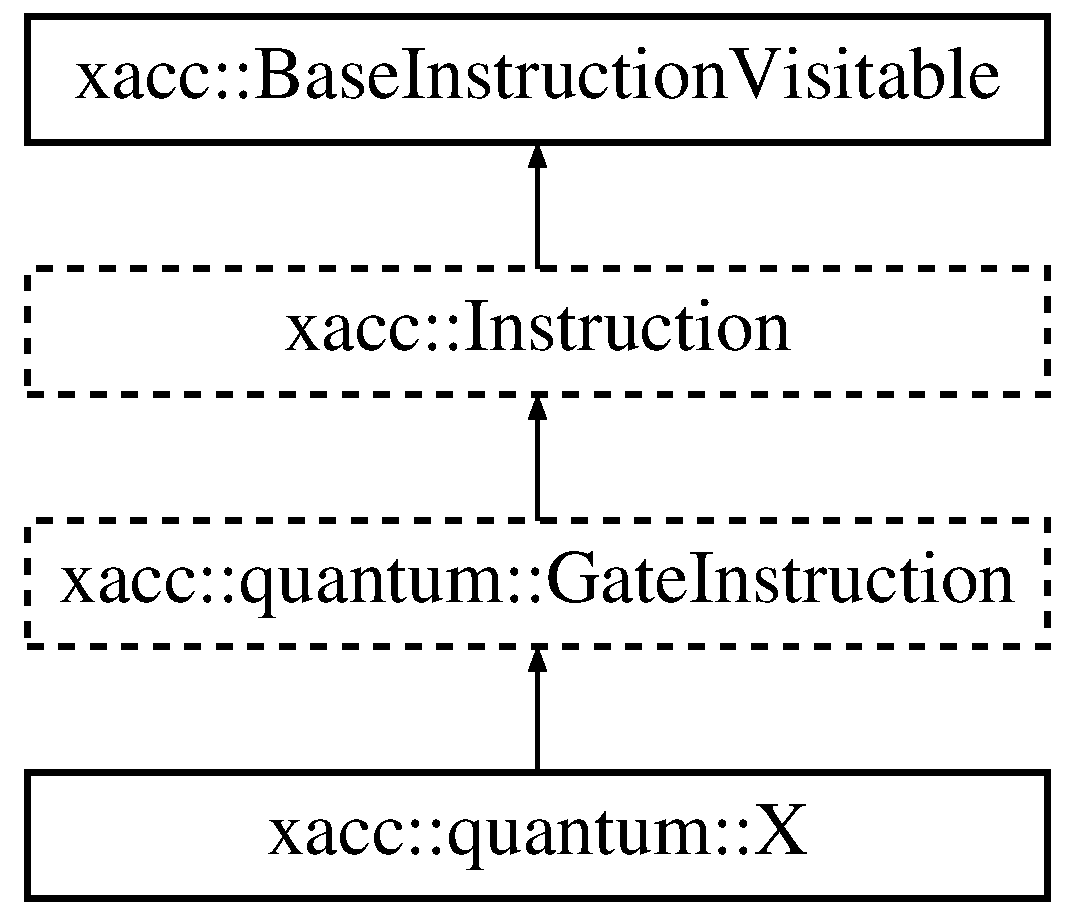
\includegraphics[height=4.000000cm]{a00070}
\end{center}
\end{figure}
\subsection*{Public Member Functions}
\begin{DoxyCompactItemize}
\item 
{\bfseries X} (std\+::vector$<$ int $>$ qbit)\hypertarget{a00070_aedc541a302602154847118f73b040510}{}\label{a00070_aedc541a302602154847118f73b040510}

\item 
{\bfseries X} (int qbit)\hypertarget{a00070_a1159bd01929b59277b4524ccfcfd7440}{}\label{a00070_a1159bd01929b59277b4524ccfcfd7440}

\end{DoxyCompactItemize}
\subsection*{Additional Inherited Members}


The documentation for this class was generated from the following files\+:\begin{DoxyCompactItemize}
\item 
X.\+hpp\item 
X.\+cpp\end{DoxyCompactItemize}

\hypertarget{a00071}{}\section{Generic\+Value$<$ Encoding, Allocator $>$\+:\+:Data Union Reference}
\label{a00071}\index{Generic\+Value$<$ Encoding, Allocator $>$\+::\+Data@{Generic\+Value$<$ Encoding, Allocator $>$\+::\+Data}}
\subsection*{Public Attributes}
\begin{DoxyCompactItemize}
\item 
\hyperlink{a00291}{String} {\bfseries s}\hypertarget{a00071_a6872a4b93763944063b425e6c001ed2b}{}\label{a00071_a6872a4b93763944063b425e6c001ed2b}

\item 
\hyperlink{a00273}{Short\+String} {\bfseries ss}\hypertarget{a00071_a410e39a5dc296eb3b152b54193740e4c}{}\label{a00071_a410e39a5dc296eb3b152b54193740e4c}

\item 
\hyperlink{a00226}{Number} {\bfseries n}\hypertarget{a00071_a243007cce2f4b75bea3e3c1ee4c3c239}{}\label{a00071_a243007cce2f4b75bea3e3c1ee4c3c239}

\item 
\hyperlink{a00227}{Object\+Data} {\bfseries o}\hypertarget{a00071_af6417eca530fba0d8bd65d309628eb11}{}\label{a00071_af6417eca530fba0d8bd65d309628eb11}

\item 
\hyperlink{a00037}{Array\+Data} {\bfseries a}\hypertarget{a00071_aeac31cf55bf5a024cead5ecb63e4fd48}{}\label{a00071_aeac31cf55bf5a024cead5ecb63e4fd48}

\item 
\hyperlink{a00104}{Flag} {\bfseries f}\hypertarget{a00071_ad8572112da083c775ce21bcbca96b2ab}{}\label{a00071_ad8572112da083c775ce21bcbca96b2ab}

\end{DoxyCompactItemize}


The documentation for this union was generated from the following file\+:\begin{DoxyCompactItemize}
\item 
\hyperlink{a00473}{document.\+h}\end{DoxyCompactItemize}

\hypertarget{a00072}{}\section{xacc\+:\+:X\+A\+C\+C\+InfoT Class Reference}
\label{a00072}\index{xacc\+::\+X\+A\+C\+C\+InfoT@{xacc\+::\+X\+A\+C\+C\+InfoT}}
\subsection*{Static Public Member Functions}
\begin{DoxyCompactItemize}
\item 
static void {\bfseries print\+Info} (const std\+::string \&msg)\hypertarget{a00072_afa78299617677d0be1b721600b48a8fa}{}\label{a00072_afa78299617677d0be1b721600b48a8fa}

\end{DoxyCompactItemize}


The documentation for this class was generated from the following file\+:\begin{DoxyCompactItemize}
\item 
Utils.\+hpp\end{DoxyCompactItemize}

\hypertarget{a00073}{}\section{xacc\+:\+:quantum\+:\+:Rx Class Reference}
\label{a00073}\index{xacc\+::quantum\+::\+Rx@{xacc\+::quantum\+::\+Rx}}
Inheritance diagram for xacc\+:\+:quantum\+:\+:Rx\+:\begin{figure}[H]
\begin{center}
\leavevmode
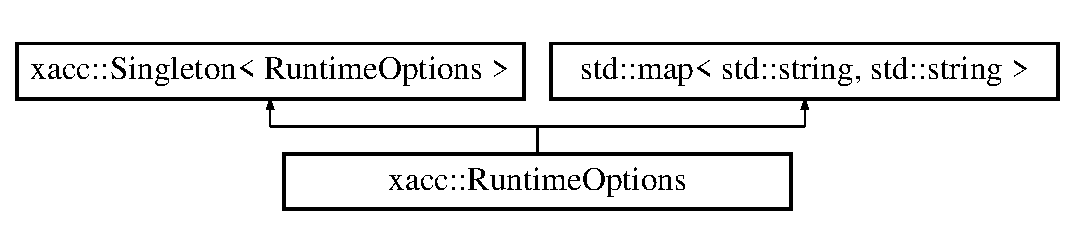
\includegraphics[height=4.000000cm]{a00073}
\end{center}
\end{figure}
\subsection*{Public Member Functions}
\begin{DoxyCompactItemize}
\item 
{\bfseries Rx} (std\+::vector$<$ int $>$ \hyperlink{a00041_a2a56be6c2519ea65df4d06f4abae1393}{qbits})\hypertarget{a00073_a03babfe938a6cbf7f744fcd31a52d92d}{}\label{a00073_a03babfe938a6cbf7f744fcd31a52d92d}

\item 
{\bfseries Rx} (int qbit, double theta)\hypertarget{a00073_a01667b11d34d5621b98ebff9a07d9bbf}{}\label{a00073_a01667b11d34d5621b98ebff9a07d9bbf}

\end{DoxyCompactItemize}
\subsection*{Additional Inherited Members}


The documentation for this class was generated from the following files\+:\begin{DoxyCompactItemize}
\item 
Rx.\+hpp\item 
Rx.\+cpp\end{DoxyCompactItemize}

\hypertarget{a00074}{}\section{xacc\+:\+:quantum\+:\+:Ry Class Reference}
\label{a00074}\index{xacc\+::quantum\+::\+Ry@{xacc\+::quantum\+::\+Ry}}
Inheritance diagram for xacc\+:\+:quantum\+:\+:Ry\+:\begin{figure}[H]
\begin{center}
\leavevmode
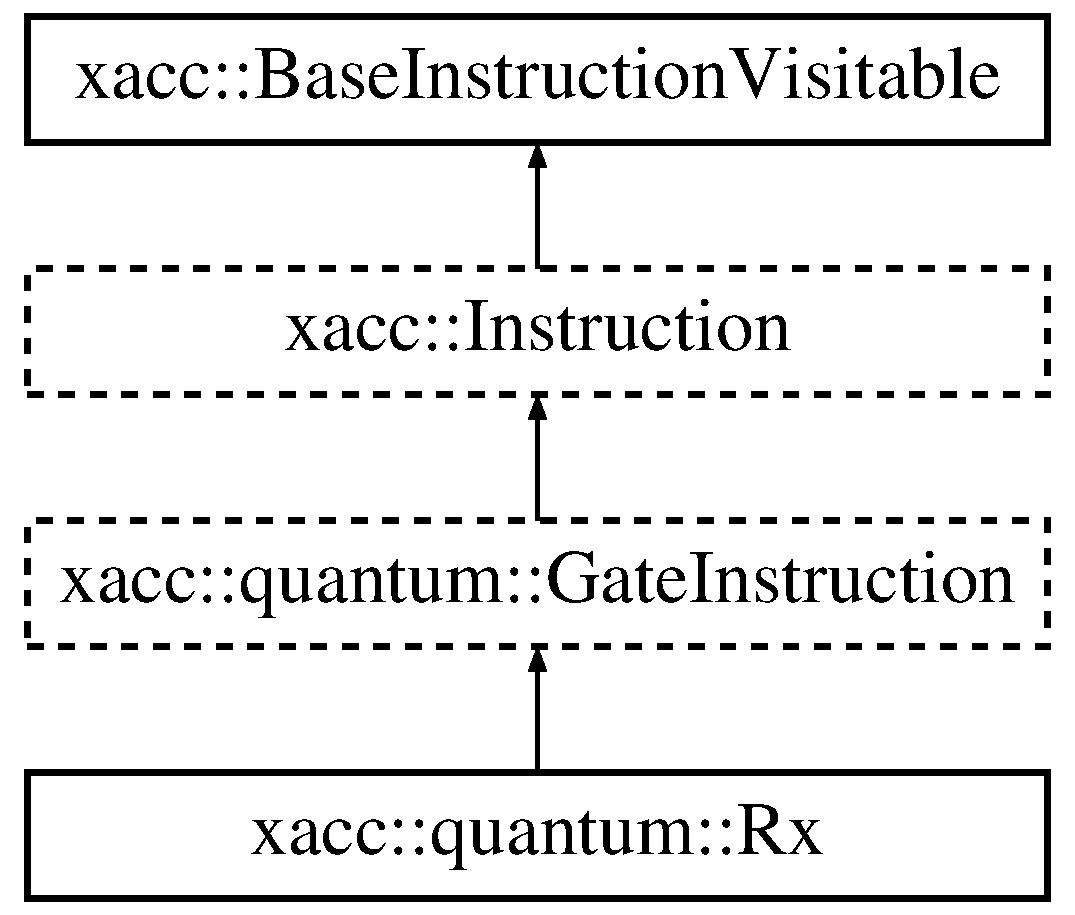
\includegraphics[height=4.000000cm]{a00074}
\end{center}
\end{figure}
\subsection*{Public Member Functions}
\begin{DoxyCompactItemize}
\item 
{\bfseries Ry} (std\+::vector$<$ int $>$ \hyperlink{a00041_a2a56be6c2519ea65df4d06f4abae1393}{qbits})\hypertarget{a00074_a542e1c0576a8e784f6cece4c77598486}{}\label{a00074_a542e1c0576a8e784f6cece4c77598486}

\item 
{\bfseries Ry} (int qbit, double theta)\hypertarget{a00074_a1cb81fe622168ba8d79fa2a78b5b0006}{}\label{a00074_a1cb81fe622168ba8d79fa2a78b5b0006}

\end{DoxyCompactItemize}
\subsection*{Additional Inherited Members}


The documentation for this class was generated from the following files\+:\begin{DoxyCompactItemize}
\item 
Ry.\+hpp\item 
Ry.\+cpp\end{DoxyCompactItemize}

\hypertarget{a00075}{}\section{xacc\+:\+:quantum\+:\+:Inverse\+Q\+FT Class Reference}
\label{a00075}\index{xacc\+::quantum\+::\+Inverse\+Q\+FT@{xacc\+::quantum\+::\+Inverse\+Q\+FT}}


{\ttfamily \#include $<$Inverse\+Q\+F\+T.\+hpp$>$}

Inheritance diagram for xacc\+:\+:quantum\+:\+:Inverse\+Q\+FT\+:\begin{figure}[H]
\begin{center}
\leavevmode
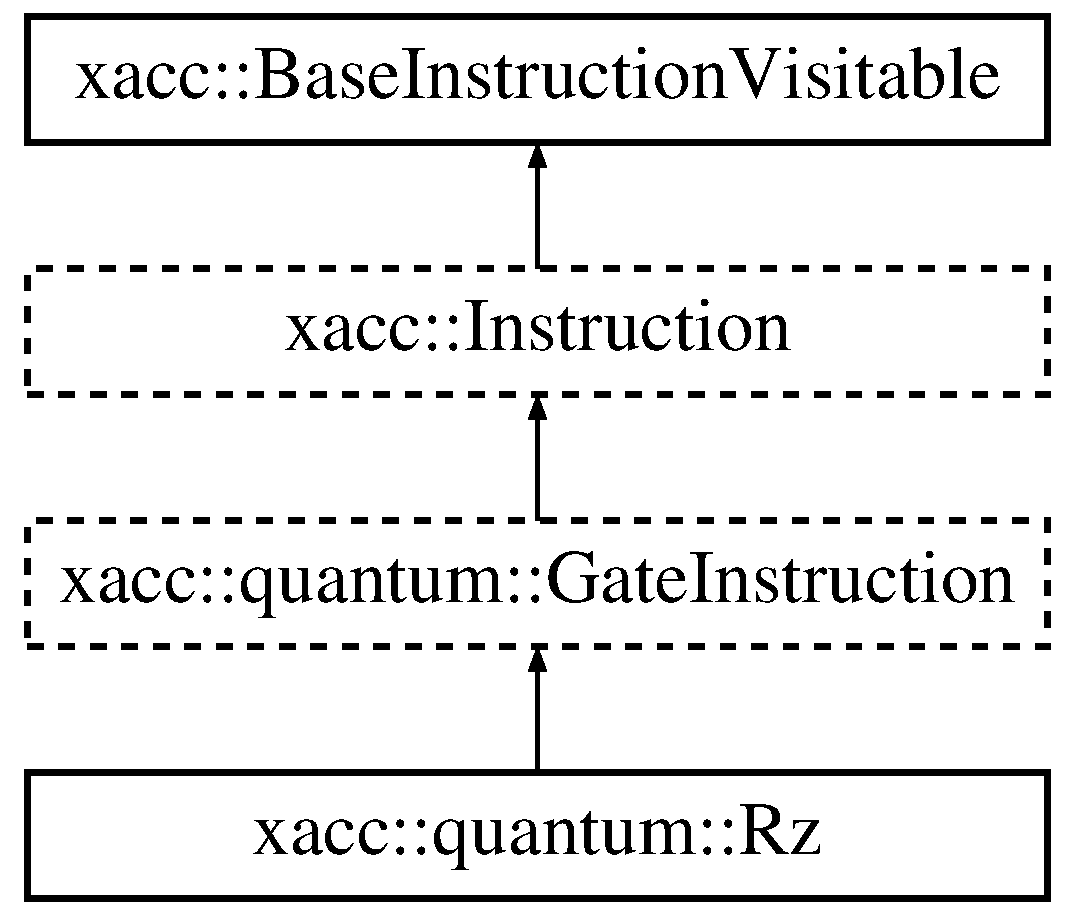
\includegraphics[height=2.000000cm]{a00075}
\end{center}
\end{figure}
\subsection*{Public Member Functions}
\begin{DoxyCompactItemize}
\item 
virtual std\+::shared\+\_\+ptr$<$ \hyperlink{a00059}{Function} $>$ \hyperlink{a00075_af42e466bf02dbd60670d20aa55cfb08d}{generate\+Algorithm} (std\+::vector$<$ int $>$ qubits)
\item 
virtual \hyperlink{a00075_a731c10d28046424be74e4c0daa31d016}{$\sim$\+Inverse\+Q\+FT} ()
\end{DoxyCompactItemize}


\subsection{Detailed Description}
\hyperlink{a00075}{Inverse\+Q\+FT} is a realization of the \hyperlink{a00020}{Algorithm\+Generator} interface that produces an X\+A\+CC \hyperlink{a00077}{IR} representation of the Inverse Quantum Fourier Transform. 

\subsection{Constructor \& Destructor Documentation}
\index{xacc\+::quantum\+::\+Inverse\+Q\+FT@{xacc\+::quantum\+::\+Inverse\+Q\+FT}!````~Inverse\+Q\+FT@{$\sim$\+Inverse\+Q\+FT}}
\index{````~Inverse\+Q\+FT@{$\sim$\+Inverse\+Q\+FT}!xacc\+::quantum\+::\+Inverse\+Q\+FT@{xacc\+::quantum\+::\+Inverse\+Q\+FT}}
\subsubsection[{\texorpdfstring{$\sim$\+Inverse\+Q\+F\+T()}{~InverseQFT()}}]{\setlength{\rightskip}{0pt plus 5cm}virtual xacc\+::quantum\+::\+Inverse\+Q\+F\+T\+::$\sim$\+Inverse\+Q\+FT (
\begin{DoxyParamCaption}
{}
\end{DoxyParamCaption}
)\hspace{0.3cm}{\ttfamily [inline]}, {\ttfamily [virtual]}}\hypertarget{a00075_a731c10d28046424be74e4c0daa31d016}{}\label{a00075_a731c10d28046424be74e4c0daa31d016}
The destructor 

\subsection{Member Function Documentation}
\index{xacc\+::quantum\+::\+Inverse\+Q\+FT@{xacc\+::quantum\+::\+Inverse\+Q\+FT}!generate\+Algorithm@{generate\+Algorithm}}
\index{generate\+Algorithm@{generate\+Algorithm}!xacc\+::quantum\+::\+Inverse\+Q\+FT@{xacc\+::quantum\+::\+Inverse\+Q\+FT}}
\subsubsection[{\texorpdfstring{generate\+Algorithm(std\+::vector$<$ int $>$ qubits)}{generateAlgorithm(std::vector< int > qubits)}}]{\setlength{\rightskip}{0pt plus 5cm}std\+::shared\+\_\+ptr$<$ {\bf Function} $>$ xacc\+::quantum\+::\+Inverse\+Q\+F\+T\+::generate\+Algorithm (
\begin{DoxyParamCaption}
\item[{std\+::vector$<$ int $>$}]{qubits}
\end{DoxyParamCaption}
)\hspace{0.3cm}{\ttfamily [virtual]}}\hypertarget{a00075_af42e466bf02dbd60670d20aa55cfb08d}{}\label{a00075_af42e466bf02dbd60670d20aa55cfb08d}
This implementation returns a \hyperlink{a00059}{Function} \hyperlink{a00077}{IR} representation of the inverse quantum fourier transform.


\begin{DoxyParams}{Parameters}
{\em bits} & The bits this algorithm operates on \\
\hline
\end{DoxyParams}
\begin{DoxyReturn}{Returns}
function The algorithm represented as an \hyperlink{a00077}{IR} \hyperlink{a00059}{Function} 
\end{DoxyReturn}


Implements \hyperlink{a00020_a73023c06f0f0c62ad56ab4187b18b096}{xacc\+::\+Algorithm\+Generator}.



The documentation for this class was generated from the following files\+:\begin{DoxyCompactItemize}
\item 
Inverse\+Q\+F\+T.\+hpp\item 
Inverse\+Q\+F\+T.\+cpp\end{DoxyCompactItemize}

\hypertarget{a00076}{}\section{boost\+:\+:dll\+:\+:detail\+:\+:destructor$<$ Class $>$ Struct Template Reference}
\label{a00076}\index{boost\+::dll\+::detail\+::destructor$<$ Class $>$@{boost\+::dll\+::detail\+::destructor$<$ Class $>$}}
\subsection*{Public Types}
\begin{DoxyCompactItemize}
\item 
typedef void($\ast$ {\bfseries type}) (Class $\ast$const)\hypertarget{a00076_a155dbf742e9c6499f52041d0b9f061be}{}\label{a00076_a155dbf742e9c6499f52041d0b9f061be}

\item 
typedef type {\bfseries standard\+\_\+t}\hypertarget{a00076_a6a72bebfcaef05b746a9b4cf93d66c50}{}\label{a00076_a6a72bebfcaef05b746a9b4cf93d66c50}

\item 
typedef type {\bfseries deleting\+\_\+t}\hypertarget{a00076_aff7ad402a5e8d7c8d1d086f73f3acf88}{}\label{a00076_aff7ad402a5e8d7c8d1d086f73f3acf88}

\end{DoxyCompactItemize}
\subsection*{Public Member Functions}
\begin{DoxyCompactItemize}
\item 
void \hyperlink{a00076_a95d55018849080c7d4c771b564e9b04e}{call\+\_\+standard} (Class $\ast$const ptr)\hypertarget{a00076_a95d55018849080c7d4c771b564e9b04e}{}\label{a00076_a95d55018849080c7d4c771b564e9b04e}

\begin{DoxyCompactList}\small\item\em Call the standard contructor. \end{DoxyCompactList}\item 
void \hyperlink{a00076_aabc107ff82b8a6f7e5aed5bd84080b1f}{call\+\_\+deleting} (Class $\ast$const ptr)\hypertarget{a00076_aabc107ff82b8a6f7e5aed5bd84080b1f}{}\label{a00076_aabc107ff82b8a6f7e5aed5bd84080b1f}

\begin{DoxyCompactList}\small\item\em Call the deleting destructor. \end{DoxyCompactList}\item 
bool \hyperlink{a00076_a294eee52606f8fdfbff528adbc50c3ea}{has\+\_\+deleting} () const \hypertarget{a00076_a294eee52606f8fdfbff528adbc50c3ea}{}\label{a00076_a294eee52606f8fdfbff528adbc50c3ea}

\begin{DoxyCompactList}\small\item\em True if a deleting destructor could be loaded. \end{DoxyCompactList}\item 
bool \hyperlink{a00076_a3efe4b3476a9157740a5a8840ae39186}{has\+\_\+standard} () const \hypertarget{a00076_a3efe4b3476a9157740a5a8840ae39186}{}\label{a00076_a3efe4b3476a9157740a5a8840ae39186}

\begin{DoxyCompactList}\small\item\em True if a standard destructor could be loaded. \end{DoxyCompactList}\item 
bool \hyperlink{a00076_adf4ce5f7e9d65a0ec22abf8109f0a5c3}{is\+\_\+empty} () const \hypertarget{a00076_adf4ce5f7e9d65a0ec22abf8109f0a5c3}{}\label{a00076_adf4ce5f7e9d65a0ec22abf8109f0a5c3}

\begin{DoxyCompactList}\small\item\em False if neither the deleting nor the standard destructor is available. \end{DoxyCompactList}\item 
\hyperlink{a00076_a45248a911612597c871150e12ad3208b}{destructor} (const \hyperlink{a00076}{destructor} \&)=default\hypertarget{a00076_a45248a911612597c871150e12ad3208b}{}\label{a00076_a45248a911612597c871150e12ad3208b}

\begin{DoxyCompactList}\small\item\em Copy destructor. \end{DoxyCompactList}\item 
\hyperlink{a00076_abc1f0cdcc708f43049b7d11727e24f24}{destructor} (const standard\+\_\+t \&\hyperlink{a00076_a5c588780f2142ca3492ea78c62fe472c}{standard}, const deleting\+\_\+t \&\hyperlink{a00076_a96ad279626c7f9b845d47582f9f88dc0}{deleting}=nullptr)\hypertarget{a00076_abc1f0cdcc708f43049b7d11727e24f24}{}\label{a00076_abc1f0cdcc708f43049b7d11727e24f24}

\begin{DoxyCompactList}\small\item\em Construct it from both the standard destructor and the allocating destructor. \end{DoxyCompactList}\end{DoxyCompactItemize}
\subsection*{Public Attributes}
\begin{DoxyCompactItemize}
\item 
standard\+\_\+t \hyperlink{a00076_a5c588780f2142ca3492ea78c62fe472c}{standard}
\begin{DoxyCompactList}\small\item\em The standard, i.\+e. not deleting destructor. \end{DoxyCompactList}\item 
deleting\+\_\+t \hyperlink{a00076_a96ad279626c7f9b845d47582f9f88dc0}{deleting}
\begin{DoxyCompactList}\small\item\em The deleting destructor. \end{DoxyCompactList}\end{DoxyCompactItemize}


\subsection{Member Data Documentation}
\index{boost\+::dll\+::detail\+::destructor@{boost\+::dll\+::detail\+::destructor}!deleting@{deleting}}
\index{deleting@{deleting}!boost\+::dll\+::detail\+::destructor@{boost\+::dll\+::detail\+::destructor}}
\subsubsection[{\texorpdfstring{deleting}{deleting}}]{\setlength{\rightskip}{0pt plus 5cm}template$<$typename Class$>$ deleting\+\_\+t {\bf boost\+::dll\+::detail\+::destructor}$<$ Class $>$\+::deleting}\hypertarget{a00076_a96ad279626c7f9b845d47582f9f88dc0}{}\label{a00076_a96ad279626c7f9b845d47582f9f88dc0}


The deleting destructor. 

\begin{DoxyWarning}{Warning}
May differ with the compiler. Use destructor\+::call\+\_\+deallocating instead. 
\end{DoxyWarning}
\index{boost\+::dll\+::detail\+::destructor@{boost\+::dll\+::detail\+::destructor}!standard@{standard}}
\index{standard@{standard}!boost\+::dll\+::detail\+::destructor@{boost\+::dll\+::detail\+::destructor}}
\subsubsection[{\texorpdfstring{standard}{standard}}]{\setlength{\rightskip}{0pt plus 5cm}template$<$typename Class$>$ standard\+\_\+t {\bf boost\+::dll\+::detail\+::destructor}$<$ Class $>$\+::standard}\hypertarget{a00076_a5c588780f2142ca3492ea78c62fe472c}{}\label{a00076_a5c588780f2142ca3492ea78c62fe472c}


The standard, i.\+e. not deleting destructor. 

\begin{DoxyWarning}{Warning}
May differ with the compiler. Use \hyperlink{a00076_a95d55018849080c7d4c771b564e9b04e}{destructor\+::call\+\_\+standard} instead. 
\end{DoxyWarning}


The documentation for this struct was generated from the following file\+:\begin{DoxyCompactItemize}
\item 
ctor\+\_\+dtor.\+hpp\end{DoxyCompactItemize}

\hypertarget{a00077}{}\section{xacc\+:\+:IR Class Reference}
\label{a00077}\index{xacc\+::\+IR@{xacc\+::\+IR}}


{\ttfamily \#include $<$I\+R.\+hpp$>$}

Inheritance diagram for xacc\+:\+:IR\+:\begin{figure}[H]
\begin{center}
\leavevmode
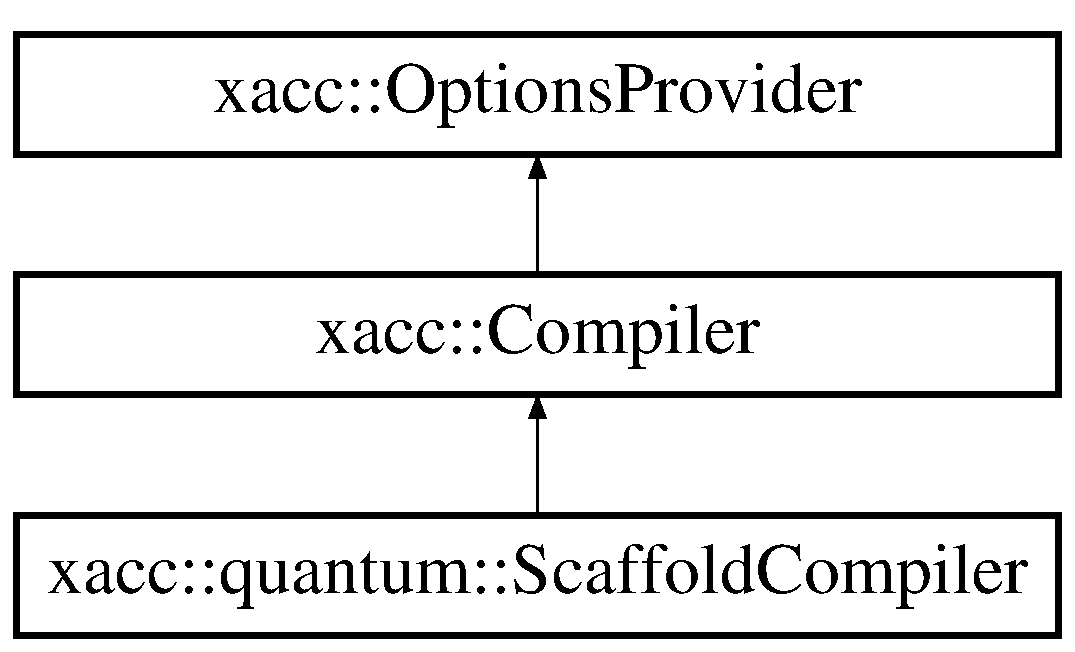
\includegraphics[height=2.000000cm]{a00077}
\end{center}
\end{figure}
\subsection*{Public Member Functions}
\begin{DoxyCompactItemize}
\item 
virtual std\+::string \hyperlink{a00077_a8356cdff1919b88eabeb84fd7450cdb6}{to\+Assembly\+String} (const std\+::string \&kernel\+Name, const std\+::string \&acc\+Buffer\+Var\+Name)=0
\item 
virtual void \hyperlink{a00077_a414b72224d88473ad6190bb88102a3ea}{persist} (std\+::ostream \&out\+Stream)=0
\item 
virtual void \hyperlink{a00077_a444c2e4dc0faac500fb70fa93997e9bc}{load} (std\+::istream \&in\+Stream)=0
\item 
virtual void \hyperlink{a00077_abbbf8e6993c518597de32cd05d49d737}{add\+Kernel} (std\+::shared\+\_\+ptr$<$ \hyperlink{a00059}{Function} $>$ kernel)=0
\item 
virtual bool \hyperlink{a00077_afc9ccf5126f3fed19c2e879133b2f6d8}{kernel\+Exists} (const std\+::string \&name)=0
\item 
virtual std\+::shared\+\_\+ptr$<$ \hyperlink{a00059}{Function} $>$ \hyperlink{a00077_a6f49b4ba4b3a15142b04873284885f0d}{get\+Kernel} (const std\+::string \&name)=0
\item 
virtual std\+::vector$<$ std\+::shared\+\_\+ptr$<$ \hyperlink{a00059}{Function} $>$ $>$ \hyperlink{a00077_a88c50bfc5b279145360ddc0c3a703b9b}{get\+Kernels} ()=0
\item 
virtual \hyperlink{a00077_a09a76d71092254acae07e19fa2f34921}{$\sim$\+IR} ()
\end{DoxyCompactItemize}


\subsection{Detailed Description}
The \hyperlink{a00077}{IR} interface is the base interface for derived accelerator-\/specific intermediate representations. At this level, an intermediate representation can be persisted to an assembly-\/like string, can be read in from file, and can be persisted to file. Since all X\+A\+CC intermediate representations operate on an \hyperlink{a00017}{Accelerator} Buffer, the \hyperlink{a00077}{IR} interface also provides a setter for such a buffer. 

\subsection{Constructor \& Destructor Documentation}
\index{xacc\+::\+IR@{xacc\+::\+IR}!````~IR@{$\sim$\+IR}}
\index{````~IR@{$\sim$\+IR}!xacc\+::\+IR@{xacc\+::\+IR}}
\subsubsection[{\texorpdfstring{$\sim$\+I\+R()}{~IR()}}]{\setlength{\rightskip}{0pt plus 5cm}virtual xacc\+::\+I\+R\+::$\sim$\+IR (
\begin{DoxyParamCaption}
{}
\end{DoxyParamCaption}
)\hspace{0.3cm}{\ttfamily [inline]}, {\ttfamily [virtual]}}\hypertarget{a00077_a09a76d71092254acae07e19fa2f34921}{}\label{a00077_a09a76d71092254acae07e19fa2f34921}
The destructor 

\subsection{Member Function Documentation}
\index{xacc\+::\+IR@{xacc\+::\+IR}!add\+Kernel@{add\+Kernel}}
\index{add\+Kernel@{add\+Kernel}!xacc\+::\+IR@{xacc\+::\+IR}}
\subsubsection[{\texorpdfstring{add\+Kernel(std\+::shared\+\_\+ptr$<$ Function $>$ kernel)=0}{addKernel(std::shared\_ptr< Function > kernel)=0}}]{\setlength{\rightskip}{0pt plus 5cm}virtual void xacc\+::\+I\+R\+::add\+Kernel (
\begin{DoxyParamCaption}
\item[{std\+::shared\+\_\+ptr$<$ {\bf Function} $>$}]{kernel}
\end{DoxyParamCaption}
)\hspace{0.3cm}{\ttfamily [pure virtual]}}\hypertarget{a00077_abbbf8e6993c518597de32cd05d49d737}{}\label{a00077_abbbf8e6993c518597de32cd05d49d737}
Add a new kernel to this \hyperlink{a00077}{IR} instance.


\begin{DoxyParams}{Parameters}
{\em kernel} & The \hyperlink{a00059}{Function} instance to add as a new kernel \\
\hline
\end{DoxyParams}


Implemented in \hyperlink{a00063_aa6ed2cf2cbcfec8105c327a4fa95346f}{xacc\+::quantum\+::\+Gate\+Q\+IR}, and \hyperlink{a00044_af1bef18e1e9568d1313b03149aab8c1b}{xacc\+::quantum\+::\+D\+W\+IR}.

\index{xacc\+::\+IR@{xacc\+::\+IR}!get\+Kernel@{get\+Kernel}}
\index{get\+Kernel@{get\+Kernel}!xacc\+::\+IR@{xacc\+::\+IR}}
\subsubsection[{\texorpdfstring{get\+Kernel(const std\+::string \&name)=0}{getKernel(const std::string \&name)=0}}]{\setlength{\rightskip}{0pt plus 5cm}virtual std\+::shared\+\_\+ptr$<${\bf Function}$>$ xacc\+::\+I\+R\+::get\+Kernel (
\begin{DoxyParamCaption}
\item[{const std\+::string \&}]{name}
\end{DoxyParamCaption}
)\hspace{0.3cm}{\ttfamily [pure virtual]}}\hypertarget{a00077_a6f49b4ba4b3a15142b04873284885f0d}{}\label{a00077_a6f49b4ba4b3a15142b04873284885f0d}
Return the kernel with the given name.


\begin{DoxyParams}{Parameters}
{\em name} & The name of the kernel to return. \\
\hline
\end{DoxyParams}
\begin{DoxyReturn}{Returns}
kernel The kernel with given name. 
\end{DoxyReturn}


Implemented in \hyperlink{a00063_a194758b6edcc3ae0c7fe8004f9bfe690}{xacc\+::quantum\+::\+Gate\+Q\+IR}, and \hyperlink{a00044_a38d8bdd24250749bc38ad31f8512fcfc}{xacc\+::quantum\+::\+D\+W\+IR}.

\index{xacc\+::\+IR@{xacc\+::\+IR}!get\+Kernels@{get\+Kernels}}
\index{get\+Kernels@{get\+Kernels}!xacc\+::\+IR@{xacc\+::\+IR}}
\subsubsection[{\texorpdfstring{get\+Kernels()=0}{getKernels()=0}}]{\setlength{\rightskip}{0pt plus 5cm}virtual std\+::vector$<$std\+::shared\+\_\+ptr$<${\bf Function}$>$ $>$ xacc\+::\+I\+R\+::get\+Kernels (
\begin{DoxyParamCaption}
{}
\end{DoxyParamCaption}
)\hspace{0.3cm}{\ttfamily [pure virtual]}}\hypertarget{a00077_a88c50bfc5b279145360ddc0c3a703b9b}{}\label{a00077_a88c50bfc5b279145360ddc0c3a703b9b}
Return all of this \hyperlink{a00077}{IR} instance\textquotesingle{}s kernels.

\begin{DoxyReturn}{Returns}
kernels The kernels this \hyperlink{a00077}{IR} contains. 
\end{DoxyReturn}


Implemented in \hyperlink{a00063_a4ace7ee5ebef84b1f39aaf5ed12c6cc6}{xacc\+::quantum\+::\+Gate\+Q\+IR}, and \hyperlink{a00044_a66e22c5dc95ec46045476864012ad08f}{xacc\+::quantum\+::\+D\+W\+IR}.

\index{xacc\+::\+IR@{xacc\+::\+IR}!kernel\+Exists@{kernel\+Exists}}
\index{kernel\+Exists@{kernel\+Exists}!xacc\+::\+IR@{xacc\+::\+IR}}
\subsubsection[{\texorpdfstring{kernel\+Exists(const std\+::string \&name)=0}{kernelExists(const std::string \&name)=0}}]{\setlength{\rightskip}{0pt plus 5cm}virtual bool xacc\+::\+I\+R\+::kernel\+Exists (
\begin{DoxyParamCaption}
\item[{const std\+::string \&}]{name}
\end{DoxyParamCaption}
)\hspace{0.3cm}{\ttfamily [pure virtual]}}\hypertarget{a00077_afc9ccf5126f3fed19c2e879133b2f6d8}{}\label{a00077_afc9ccf5126f3fed19c2e879133b2f6d8}
Return true if the kernel with given name exists in this \hyperlink{a00077}{IR}.


\begin{DoxyParams}{Parameters}
{\em name} & The name of the kernel to return. \\
\hline
\end{DoxyParams}
\begin{DoxyReturn}{Returns}
exists True if kernel exists. 
\end{DoxyReturn}


Implemented in \hyperlink{a00063_a692f95099caa7c024110a3f035941dca}{xacc\+::quantum\+::\+Gate\+Q\+IR}, and \hyperlink{a00044_ab5e8861d3bc0845bb015af6208f5f396}{xacc\+::quantum\+::\+D\+W\+IR}.

\index{xacc\+::\+IR@{xacc\+::\+IR}!load@{load}}
\index{load@{load}!xacc\+::\+IR@{xacc\+::\+IR}}
\subsubsection[{\texorpdfstring{load(std\+::istream \&in\+Stream)=0}{load(std::istream \&inStream)=0}}]{\setlength{\rightskip}{0pt plus 5cm}virtual void xacc\+::\+I\+R\+::load (
\begin{DoxyParamCaption}
\item[{std\+::istream \&}]{in\+Stream}
\end{DoxyParamCaption}
)\hspace{0.3cm}{\ttfamily [pure virtual]}}\hypertarget{a00077_a444c2e4dc0faac500fb70fa93997e9bc}{}\label{a00077_a444c2e4dc0faac500fb70fa93997e9bc}
Create this \hyperlink{a00077}{IR} instance from the given input stream.


\begin{DoxyParams}{Parameters}
{\em in\+Stream} & The input stream to read from. \\
\hline
\end{DoxyParams}


Implemented in \hyperlink{a00063_a07f26eeb362ac480d20da6cdc8c8fb39}{xacc\+::quantum\+::\+Gate\+Q\+IR}, and \hyperlink{a00044_a8b388d719d565bb902c979807d3d0d47}{xacc\+::quantum\+::\+D\+W\+IR}.

\index{xacc\+::\+IR@{xacc\+::\+IR}!persist@{persist}}
\index{persist@{persist}!xacc\+::\+IR@{xacc\+::\+IR}}
\subsubsection[{\texorpdfstring{persist(std\+::ostream \&out\+Stream)=0}{persist(std::ostream \&outStream)=0}}]{\setlength{\rightskip}{0pt plus 5cm}virtual void xacc\+::\+I\+R\+::persist (
\begin{DoxyParamCaption}
\item[{std\+::ostream \&}]{out\+Stream}
\end{DoxyParamCaption}
)\hspace{0.3cm}{\ttfamily [pure virtual]}}\hypertarget{a00077_a414b72224d88473ad6190bb88102a3ea}{}\label{a00077_a414b72224d88473ad6190bb88102a3ea}
Persist this \hyperlink{a00077}{IR} instance to the given output stream.


\begin{DoxyParams}{Parameters}
{\em out\+Stream} & The output stream to persist to. \\
\hline
\end{DoxyParams}


Implemented in \hyperlink{a00063_a40e1d07e4dfd3794ef53fca3cdbdca61}{xacc\+::quantum\+::\+Gate\+Q\+IR}, and \hyperlink{a00044_abcbfd0a4cf697843391c65cbd9a82080}{xacc\+::quantum\+::\+D\+W\+IR}.

\index{xacc\+::\+IR@{xacc\+::\+IR}!to\+Assembly\+String@{to\+Assembly\+String}}
\index{to\+Assembly\+String@{to\+Assembly\+String}!xacc\+::\+IR@{xacc\+::\+IR}}
\subsubsection[{\texorpdfstring{to\+Assembly\+String(const std\+::string \&kernel\+Name, const std\+::string \&acc\+Buffer\+Var\+Name)=0}{toAssemblyString(const std::string \&kernelName, const std::string \&accBufferVarName)=0}}]{\setlength{\rightskip}{0pt plus 5cm}virtual std\+::string xacc\+::\+I\+R\+::to\+Assembly\+String (
\begin{DoxyParamCaption}
\item[{const std\+::string \&}]{kernel\+Name, }
\item[{const std\+::string \&}]{acc\+Buffer\+Var\+Name}
\end{DoxyParamCaption}
)\hspace{0.3cm}{\ttfamily [pure virtual]}}\hypertarget{a00077_a8356cdff1919b88eabeb84fd7450cdb6}{}\label{a00077_a8356cdff1919b88eabeb84fd7450cdb6}
Return a assembly-\/like string representation of this intermediate representation


\begin{DoxyParams}{Parameters}
{\em kernel\+Name} & The name of hte kernel to persist to string \\
\hline
{\em acc\+Buffer\+Var\+Name} & The name of the \hyperlink{a00019}{Accelerator\+Buffer} \\
\hline
\end{DoxyParams}
\begin{DoxyReturn}{Returns}

\end{DoxyReturn}


Implemented in \hyperlink{a00063_a7153f7e9f516d43af3d5d4f95d60bd86}{xacc\+::quantum\+::\+Gate\+Q\+IR}, and \hyperlink{a00044_a880cb60197577ea31115331e3a030e3e}{xacc\+::quantum\+::\+D\+W\+IR}.



The documentation for this class was generated from the following file\+:\begin{DoxyCompactItemize}
\item 
I\+R.\+hpp\end{DoxyCompactItemize}

\hypertarget{a00078}{}\section{xacc\+:\+:quantum\+:\+:Scaffold\+Compiler Class Reference}
\label{a00078}\index{xacc\+::quantum\+::\+Scaffold\+Compiler@{xacc\+::quantum\+::\+Scaffold\+Compiler}}


{\ttfamily \#include $<$Scaffold\+Compiler.\+hpp$>$}

Inheritance diagram for xacc\+:\+:quantum\+:\+:Scaffold\+Compiler\+:\begin{figure}[H]
\begin{center}
\leavevmode
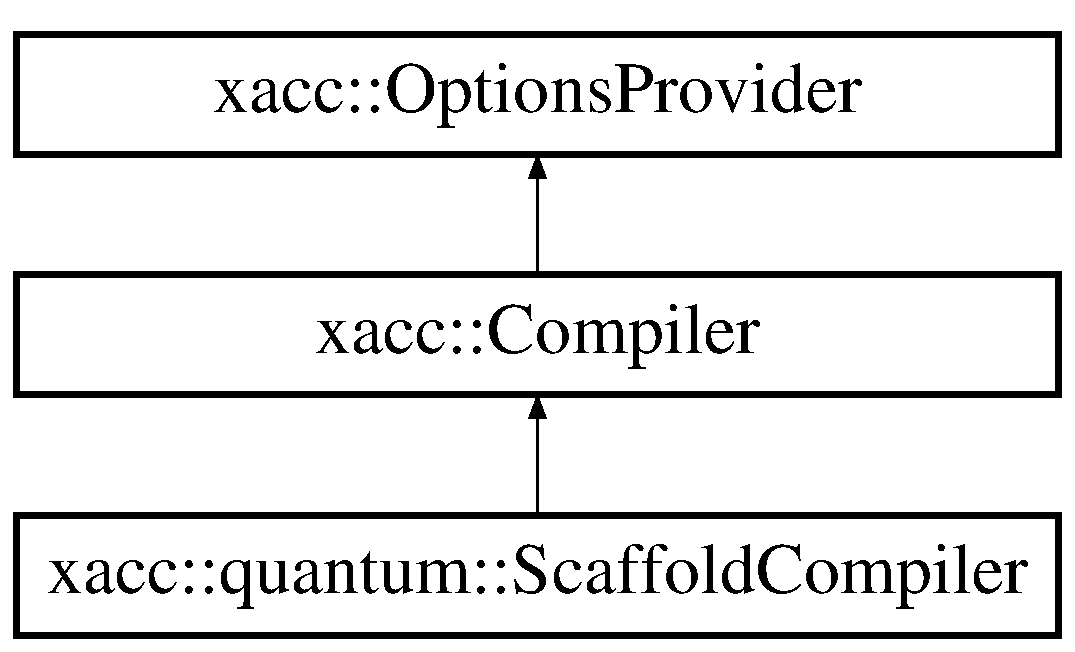
\includegraphics[height=3.000000cm]{a00078}
\end{center}
\end{figure}
\subsection*{Public Member Functions}
\begin{DoxyCompactItemize}
\item 
virtual std\+::shared\+\_\+ptr$<$ \hyperlink{a00051}{xacc\+::\+IR} $>$ \hyperlink{a00078_a7caede75bb2304ba405966651b115543}{compile} (const std\+::string \&src, std\+::shared\+\_\+ptr$<$ \hyperlink{a00011}{Accelerator} $>$ acc)
\item 
virtual std\+::shared\+\_\+ptr$<$ \hyperlink{a00051}{xacc\+::\+IR} $>$ \hyperlink{a00078_a3736ecc229fe6acdd4c991e85d7a1f08}{compile} (const std\+::string \&src)
\item 
virtual const std\+::string \hyperlink{a00078_ac7ca2941e987ba579c6f50cfbd7fb0dc}{translate} (const std\+::string \&buffer\+Variable, std\+::shared\+\_\+ptr$<$ \hyperlink{a00039}{Function} $>$ function)
\item 
virtual const std\+::string \hyperlink{a00078_a3f537054a3924a1d14f4ceb0f0181161}{get\+Name} ()
\item 
virtual \hyperlink{a00078_afb26398b07377ab9ddebc43a9376a6dd}{$\sim$\+Scaffold\+Compiler} ()
\end{DoxyCompactItemize}
\subsection*{Static Public Member Functions}
\begin{DoxyCompactItemize}
\item 
static void \hyperlink{a00078_aed16dda1e919e5af6de9953a656f62ce}{register\+Compiler} ()
\end{DoxyCompactItemize}
\subsection*{Protected Attributes}
\begin{DoxyCompactItemize}
\item 
std\+::shared\+\_\+ptr$<$ clang\+::\+Compiler\+Instance $>$ \hyperlink{a00078_af7a3a73eaab025a0ea72cc9335d8fbb4}{CI}
\item 
std\+::shared\+\_\+ptr$<$ \hyperlink{a00077}{Scaffold\+A\+S\+T\+Consumer} $>$ \hyperlink{a00078_ab1c4d36e58b97de50208e74a92d8ceb1}{consumer}
\end{DoxyCompactItemize}


\subsection{Detailed Description}
The Scaffold compiler is a subclass of the X\+A\+CC \hyperlink{a00023}{Compiler} that implements the \hyperlink{a00078_a7caede75bb2304ba405966651b115543}{compile()} and modify\+Source() methods to handle generation of quantum assembly language (or Q\+A\+SM) using an installed Scaffold compiler. 

\subsection{Constructor \& Destructor Documentation}
\index{xacc\+::quantum\+::\+Scaffold\+Compiler@{xacc\+::quantum\+::\+Scaffold\+Compiler}!````~Scaffold\+Compiler@{$\sim$\+Scaffold\+Compiler}}
\index{````~Scaffold\+Compiler@{$\sim$\+Scaffold\+Compiler}!xacc\+::quantum\+::\+Scaffold\+Compiler@{xacc\+::quantum\+::\+Scaffold\+Compiler}}
\subsubsection[{\texorpdfstring{$\sim$\+Scaffold\+Compiler()}{~ScaffoldCompiler()}}]{\setlength{\rightskip}{0pt plus 5cm}virtual xacc\+::quantum\+::\+Scaffold\+Compiler\+::$\sim$\+Scaffold\+Compiler (
\begin{DoxyParamCaption}
{}
\end{DoxyParamCaption}
)\hspace{0.3cm}{\ttfamily [inline]}, {\ttfamily [virtual]}}\hypertarget{a00078_afb26398b07377ab9ddebc43a9376a6dd}{}\label{a00078_afb26398b07377ab9ddebc43a9376a6dd}
The destructor 

\subsection{Member Function Documentation}
\index{xacc\+::quantum\+::\+Scaffold\+Compiler@{xacc\+::quantum\+::\+Scaffold\+Compiler}!compile@{compile}}
\index{compile@{compile}!xacc\+::quantum\+::\+Scaffold\+Compiler@{xacc\+::quantum\+::\+Scaffold\+Compiler}}
\subsubsection[{\texorpdfstring{compile(const std\+::string \&src, std\+::shared\+\_\+ptr$<$ Accelerator $>$ acc)}{compile(const std::string \&src, std::shared\_ptr< Accelerator > acc)}}]{\setlength{\rightskip}{0pt plus 5cm}std\+::shared\+\_\+ptr$<$ {\bf IR} $>$ xacc\+::quantum\+::\+Scaffold\+Compiler\+::compile (
\begin{DoxyParamCaption}
\item[{const std\+::string \&}]{src, }
\item[{std\+::shared\+\_\+ptr$<$ {\bf Accelerator} $>$}]{acc}
\end{DoxyParamCaption}
)\hspace{0.3cm}{\ttfamily [virtual]}}\hypertarget{a00078_a7caede75bb2304ba405966651b115543}{}\label{a00078_a7caede75bb2304ba405966651b115543}
Execute the Scaffold compiler to generate an X\+A\+CC intermediate representation instance. \begin{DoxyReturn}{Returns}
ir X\+A\+CC intermediate representation 
\end{DoxyReturn}


Implements \hyperlink{a00023_a546a40c95bb93af6a0c0ac48dbeaffc8}{xacc\+::\+Compiler}.

\index{xacc\+::quantum\+::\+Scaffold\+Compiler@{xacc\+::quantum\+::\+Scaffold\+Compiler}!compile@{compile}}
\index{compile@{compile}!xacc\+::quantum\+::\+Scaffold\+Compiler@{xacc\+::quantum\+::\+Scaffold\+Compiler}}
\subsubsection[{\texorpdfstring{compile(const std\+::string \&src)}{compile(const std::string \&src)}}]{\setlength{\rightskip}{0pt plus 5cm}std\+::shared\+\_\+ptr$<$ {\bf IR} $>$ xacc\+::quantum\+::\+Scaffold\+Compiler\+::compile (
\begin{DoxyParamCaption}
\item[{const std\+::string \&}]{src}
\end{DoxyParamCaption}
)\hspace{0.3cm}{\ttfamily [virtual]}}\hypertarget{a00078_a3736ecc229fe6acdd4c991e85d7a1f08}{}\label{a00078_a3736ecc229fe6acdd4c991e85d7a1f08}

\begin{DoxyParams}{Parameters}
{\em src} & \\
\hline
\end{DoxyParams}
\begin{DoxyReturn}{Returns}

\end{DoxyReturn}


Implements \hyperlink{a00023_a9092f5f779b570c91569b59621280c04}{xacc\+::\+Compiler}.

\index{xacc\+::quantum\+::\+Scaffold\+Compiler@{xacc\+::quantum\+::\+Scaffold\+Compiler}!get\+Name@{get\+Name}}
\index{get\+Name@{get\+Name}!xacc\+::quantum\+::\+Scaffold\+Compiler@{xacc\+::quantum\+::\+Scaffold\+Compiler}}
\subsubsection[{\texorpdfstring{get\+Name()}{getName()}}]{\setlength{\rightskip}{0pt plus 5cm}virtual const std\+::string xacc\+::quantum\+::\+Scaffold\+Compiler\+::get\+Name (
\begin{DoxyParamCaption}
{}
\end{DoxyParamCaption}
)\hspace{0.3cm}{\ttfamily [inline]}, {\ttfamily [virtual]}}\hypertarget{a00078_a3f537054a3924a1d14f4ceb0f0181161}{}\label{a00078_a3f537054a3924a1d14f4ceb0f0181161}
Return the name of this \hyperlink{a00023}{Compiler} \begin{DoxyReturn}{Returns}
name \hyperlink{a00023}{Compiler} name 
\end{DoxyReturn}


Implements \hyperlink{a00023_a87fca9100e6462122f5b687c3a0fb3fb}{xacc\+::\+Compiler}.

\index{xacc\+::quantum\+::\+Scaffold\+Compiler@{xacc\+::quantum\+::\+Scaffold\+Compiler}!register\+Compiler@{register\+Compiler}}
\index{register\+Compiler@{register\+Compiler}!xacc\+::quantum\+::\+Scaffold\+Compiler@{xacc\+::quantum\+::\+Scaffold\+Compiler}}
\subsubsection[{\texorpdfstring{register\+Compiler()}{registerCompiler()}}]{\setlength{\rightskip}{0pt plus 5cm}static void xacc\+::quantum\+::\+Scaffold\+Compiler\+::register\+Compiler (
\begin{DoxyParamCaption}
{}
\end{DoxyParamCaption}
)\hspace{0.3cm}{\ttfamily [inline]}, {\ttfamily [static]}}\hypertarget{a00078_aed16dda1e919e5af6de9953a656f62ce}{}\label{a00078_aed16dda1e919e5af6de9953a656f62ce}
Register this \hyperlink{a00023}{Compiler} with the framework. \index{xacc\+::quantum\+::\+Scaffold\+Compiler@{xacc\+::quantum\+::\+Scaffold\+Compiler}!translate@{translate}}
\index{translate@{translate}!xacc\+::quantum\+::\+Scaffold\+Compiler@{xacc\+::quantum\+::\+Scaffold\+Compiler}}
\subsubsection[{\texorpdfstring{translate(const std\+::string \&buffer\+Variable, std\+::shared\+\_\+ptr$<$ Function $>$ function)}{translate(const std::string \&bufferVariable, std::shared\_ptr< Function > function)}}]{\setlength{\rightskip}{0pt plus 5cm}const std\+::string xacc\+::quantum\+::\+Scaffold\+Compiler\+::translate (
\begin{DoxyParamCaption}
\item[{const std\+::string \&}]{buffer\+Variable, }
\item[{std\+::shared\+\_\+ptr$<$ {\bf Function} $>$}]{function}
\end{DoxyParamCaption}
)\hspace{0.3cm}{\ttfamily [virtual]}}\hypertarget{a00078_ac7ca2941e987ba579c6f50cfbd7fb0dc}{}\label{a00078_ac7ca2941e987ba579c6f50cfbd7fb0dc}
This produces a Scaffold source code representation of the given \hyperlink{a00051}{IR} \hyperlink{a00039}{Function}


\begin{DoxyParams}{Parameters}
{\em function} & The X\+A\+CC \hyperlink{a00051}{IR} \hyperlink{a00039}{Function} to translate \\
\hline
\end{DoxyParams}
\begin{DoxyReturn}{Returns}
src The source code as a string 
\end{DoxyReturn}


Implements \hyperlink{a00023_aeedbe58a33fed29e4d7694ae743e25e7}{xacc\+::\+Compiler}.



\subsection{Member Data Documentation}
\index{xacc\+::quantum\+::\+Scaffold\+Compiler@{xacc\+::quantum\+::\+Scaffold\+Compiler}!CI@{CI}}
\index{CI@{CI}!xacc\+::quantum\+::\+Scaffold\+Compiler@{xacc\+::quantum\+::\+Scaffold\+Compiler}}
\subsubsection[{\texorpdfstring{CI}{CI}}]{\setlength{\rightskip}{0pt plus 5cm}std\+::shared\+\_\+ptr$<$clang\+::\+Compiler\+Instance$>$ xacc\+::quantum\+::\+Scaffold\+Compiler\+::\+CI\hspace{0.3cm}{\ttfamily [protected]}}\hypertarget{a00078_af7a3a73eaab025a0ea72cc9335d8fbb4}{}\label{a00078_af7a3a73eaab025a0ea72cc9335d8fbb4}
Reference to the Scaffold Clang \hyperlink{a00023}{Compiler} \index{xacc\+::quantum\+::\+Scaffold\+Compiler@{xacc\+::quantum\+::\+Scaffold\+Compiler}!consumer@{consumer}}
\index{consumer@{consumer}!xacc\+::quantum\+::\+Scaffold\+Compiler@{xacc\+::quantum\+::\+Scaffold\+Compiler}}
\subsubsection[{\texorpdfstring{consumer}{consumer}}]{\setlength{\rightskip}{0pt plus 5cm}std\+::shared\+\_\+ptr$<${\bf Scaffold\+A\+S\+T\+Consumer}$>$ xacc\+::quantum\+::\+Scaffold\+Compiler\+::consumer\hspace{0.3cm}{\ttfamily [protected]}}\hypertarget{a00078_ab1c4d36e58b97de50208e74a92d8ceb1}{}\label{a00078_ab1c4d36e58b97de50208e74a92d8ceb1}
Reference to our A\+ST Consumer, this gives us the compiled \hyperlink{a00051}{IR} \hyperlink{a00039}{Function} and the Qubit Variable Name 

The documentation for this class was generated from the following files\+:\begin{DoxyCompactItemize}
\item 
Scaffold\+Compiler.\+hpp\item 
Scaffold\+Compiler.\+cpp\end{DoxyCompactItemize}

\hypertarget{a00079}{}\section{xacc\+:\+:quantum\+:\+:Scaffold\+I\+R\+To\+Src\+Visitor Class Reference}
\label{a00079}\index{xacc\+::quantum\+::\+Scaffold\+I\+R\+To\+Src\+Visitor@{xacc\+::quantum\+::\+Scaffold\+I\+R\+To\+Src\+Visitor}}


{\ttfamily \#include $<$Scaffold\+I\+R\+To\+Src\+Visitor.\+hpp$>$}

Inheritance diagram for xacc\+:\+:quantum\+:\+:Scaffold\+I\+R\+To\+Src\+Visitor\+:\begin{figure}[H]
\begin{center}
\leavevmode
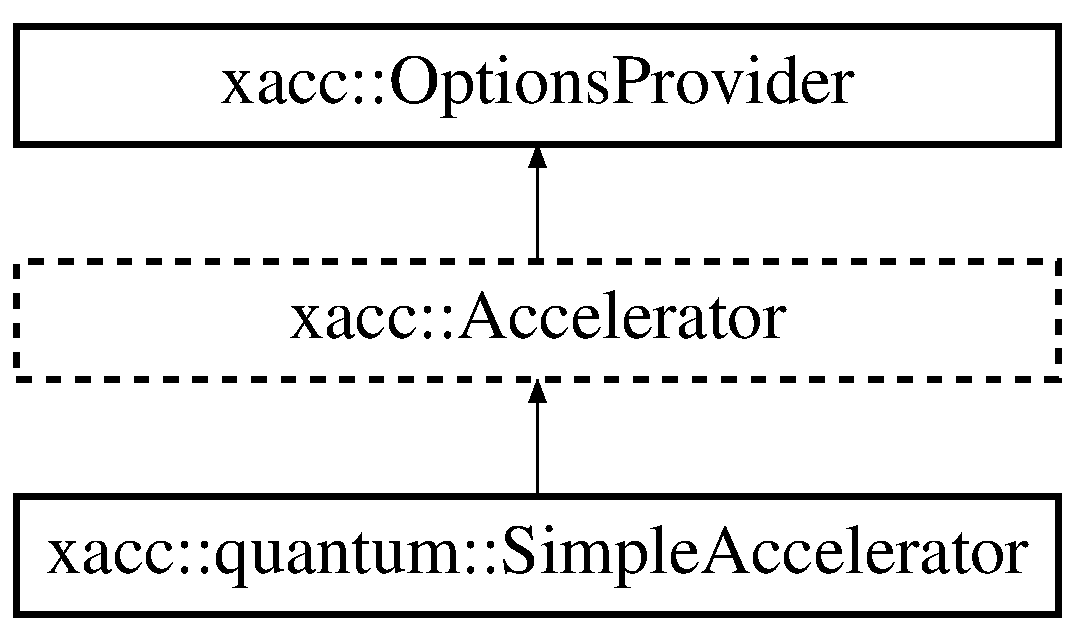
\includegraphics[height=12.000000cm]{a00079}
\end{center}
\end{figure}
\subsection*{Public Member Functions}
\begin{DoxyCompactItemize}
\item 
{\bfseries Scaffold\+I\+R\+To\+Src\+Visitor} (std\+::string var)\hypertarget{a00079_a38e9a5775397847973f78856e4b0031e}{}\label{a00079_a38e9a5775397847973f78856e4b0031e}

\item 
void \hyperlink{a00079_af66cbe08e183c8b53817cda5251d0498}{visit} (\hyperlink{a00045}{Hadamard} \&h)
\item 
void \hyperlink{a00079_a81b16c7a7da2c84174796ef4cc39b312}{visit} (\hyperlink{a00022}{C\+N\+OT} \&cn)
\item 
void \hyperlink{a00079_a1a414fa079f0e3ba8cd0f97c7928e88f}{visit} (\hyperlink{a00085}{X} \&x)
\item 
void {\bfseries visit} (\hyperlink{a00088}{Y} \&y)\hypertarget{a00079_a9130f70ceaa42bdc3c29c8b0bbdcc3b5}{}\label{a00079_a9130f70ceaa42bdc3c29c8b0bbdcc3b5}

\item 
void \hyperlink{a00079_a444936ec9134a0ea400cd2f1b145ba4d}{visit} (\hyperlink{a00089}{Z} \&z)
\item 
void \hyperlink{a00079_a99e7176144810f5d6e38d98d2725afff}{visit} (\hyperlink{a00056}{Measure} \&m)
\item 
void \hyperlink{a00079_a1646dbfaf919432c2c3d8eb86e9f81e4}{visit} (\hyperlink{a00025}{Conditional\+Function} \&c)
\item 
void {\bfseries visit} (\hyperlink{a00074}{Rx} \&rx)\hypertarget{a00079_afc1ace9f5cb4783117a68b173c069d15}{}\label{a00079_afc1ace9f5cb4783117a68b173c069d15}

\item 
void {\bfseries visit} (\hyperlink{a00075}{Ry} \&ry)\hypertarget{a00079_a08539d478a1b496244288477ccee8011}{}\label{a00079_a08539d478a1b496244288477ccee8011}

\item 
void {\bfseries visit} (\hyperlink{a00076}{Rz} \&rz)\hypertarget{a00079_a855cbf9e83b050ae65e95c4a36f02de9}{}\label{a00079_a855cbf9e83b050ae65e95c4a36f02de9}

\item 
void {\bfseries visit} (\hyperlink{a00027}{C\+Phase} \&cp)\hypertarget{a00079_a4d8e2c6d867d812aeca192ebc65a45ce}{}\label{a00079_a4d8e2c6d867d812aeca192ebc65a45ce}

\item 
void {\bfseries visit} (\hyperlink{a00083}{Swap} \&s)\hypertarget{a00079_a502e0145245e4aa00af4f76e1b201e7a}{}\label{a00079_a502e0145245e4aa00af4f76e1b201e7a}

\item 
void {\bfseries visit} (\hyperlink{a00041}{Gate\+Function} \&f)\hypertarget{a00079_adf65b4117c2dfd3242c5c214eef608c5}{}\label{a00079_adf65b4117c2dfd3242c5c214eef608c5}

\item 
std\+::string \hyperlink{a00079_ad721b67dae6360ce210d6c73feec7920}{get\+Scaffold\+String} ()
\item 
virtual \hyperlink{a00079_a366cddf574488b3bf0df1fe991806753}{$\sim$\+Scaffold\+I\+R\+To\+Src\+Visitor} ()
\end{DoxyCompactItemize}
\subsection*{Protected Member Functions}
\begin{DoxyCompactItemize}
\item 
void {\bfseries base\+Instruction} (std\+::string gate\+Name, std\+::vector$<$ int $>$ qubits)\hypertarget{a00079_afa951f637b70233cfded3c05177e2b56}{}\label{a00079_afa951f637b70233cfded3c05177e2b56}

\item 
void {\bfseries base\+Parameterized\+Instruction} (std\+::string gate\+Name, std\+::vector$<$ int $>$ qubits, std\+::vector$<$ Instruction\+Parameter $>$ params)\hypertarget{a00079_a23d8435f4696290c32afdae1abfbff30}{}\label{a00079_a23d8435f4696290c32afdae1abfbff30}

\end{DoxyCompactItemize}
\subsection*{Protected Attributes}
\begin{DoxyCompactItemize}
\item 
std\+::string \hyperlink{a00079_a4b4c3b769a275d544beb26b1894e476a}{scaffold\+Str}
\item 
std\+::string {\bfseries qubit\+Var\+Name}\hypertarget{a00079_ab538cf6fe8606e9832310a8195b67dce}{}\label{a00079_ab538cf6fe8606e9832310a8195b67dce}

\item 
int {\bfseries n\+Measurements} = 0\hypertarget{a00079_ae7d177fa9830942f63ef86fd2f69f715}{}\label{a00079_ae7d177fa9830942f63ef86fd2f69f715}

\item 
std\+::map$<$ int, int $>$ {\bfseries qubit\+To\+Classical\+Bit\+Index}\hypertarget{a00079_a76945624d8d67487d410a11a91e97681}{}\label{a00079_a76945624d8d67487d410a11a91e97681}

\end{DoxyCompactItemize}


\subsection{Detailed Description}
The \hyperlink{a00064}{Quil\+Visitor} is an \hyperlink{a00049}{Instruction\+Visitor} that visits quantum gate instructions and creates an equivalent Quil string that can be executed by the Rigetti superconducting quantum computer. 

\subsection{Constructor \& Destructor Documentation}
\index{xacc\+::quantum\+::\+Scaffold\+I\+R\+To\+Src\+Visitor@{xacc\+::quantum\+::\+Scaffold\+I\+R\+To\+Src\+Visitor}!````~Scaffold\+I\+R\+To\+Src\+Visitor@{$\sim$\+Scaffold\+I\+R\+To\+Src\+Visitor}}
\index{````~Scaffold\+I\+R\+To\+Src\+Visitor@{$\sim$\+Scaffold\+I\+R\+To\+Src\+Visitor}!xacc\+::quantum\+::\+Scaffold\+I\+R\+To\+Src\+Visitor@{xacc\+::quantum\+::\+Scaffold\+I\+R\+To\+Src\+Visitor}}
\subsubsection[{\texorpdfstring{$\sim$\+Scaffold\+I\+R\+To\+Src\+Visitor()}{~ScaffoldIRToSrcVisitor()}}]{\setlength{\rightskip}{0pt plus 5cm}virtual xacc\+::quantum\+::\+Scaffold\+I\+R\+To\+Src\+Visitor\+::$\sim$\+Scaffold\+I\+R\+To\+Src\+Visitor (
\begin{DoxyParamCaption}
{}
\end{DoxyParamCaption}
)\hspace{0.3cm}{\ttfamily [inline]}, {\ttfamily [virtual]}}\hypertarget{a00079_a366cddf574488b3bf0df1fe991806753}{}\label{a00079_a366cddf574488b3bf0df1fe991806753}
The destructor 

\subsection{Member Function Documentation}
\index{xacc\+::quantum\+::\+Scaffold\+I\+R\+To\+Src\+Visitor@{xacc\+::quantum\+::\+Scaffold\+I\+R\+To\+Src\+Visitor}!get\+Scaffold\+String@{get\+Scaffold\+String}}
\index{get\+Scaffold\+String@{get\+Scaffold\+String}!xacc\+::quantum\+::\+Scaffold\+I\+R\+To\+Src\+Visitor@{xacc\+::quantum\+::\+Scaffold\+I\+R\+To\+Src\+Visitor}}
\subsubsection[{\texorpdfstring{get\+Scaffold\+String()}{getScaffoldString()}}]{\setlength{\rightskip}{0pt plus 5cm}std\+::string xacc\+::quantum\+::\+Scaffold\+I\+R\+To\+Src\+Visitor\+::get\+Scaffold\+String (
\begin{DoxyParamCaption}
{}
\end{DoxyParamCaption}
)\hspace{0.3cm}{\ttfamily [inline]}}\hypertarget{a00079_ad721b67dae6360ce210d6c73feec7920}{}\label{a00079_ad721b67dae6360ce210d6c73feec7920}
Return the quil string \index{xacc\+::quantum\+::\+Scaffold\+I\+R\+To\+Src\+Visitor@{xacc\+::quantum\+::\+Scaffold\+I\+R\+To\+Src\+Visitor}!visit@{visit}}
\index{visit@{visit}!xacc\+::quantum\+::\+Scaffold\+I\+R\+To\+Src\+Visitor@{xacc\+::quantum\+::\+Scaffold\+I\+R\+To\+Src\+Visitor}}
\subsubsection[{\texorpdfstring{visit(\+Hadamard \&h)}{visit(Hadamard \&h)}}]{\setlength{\rightskip}{0pt plus 5cm}void xacc\+::quantum\+::\+Scaffold\+I\+R\+To\+Src\+Visitor\+::visit (
\begin{DoxyParamCaption}
\item[{{\bf Hadamard} \&}]{h}
\end{DoxyParamCaption}
)\hspace{0.3cm}{\ttfamily [inline]}}\hypertarget{a00079_af66cbe08e183c8b53817cda5251d0498}{}\label{a00079_af66cbe08e183c8b53817cda5251d0498}
Visit hadamard gates \index{xacc\+::quantum\+::\+Scaffold\+I\+R\+To\+Src\+Visitor@{xacc\+::quantum\+::\+Scaffold\+I\+R\+To\+Src\+Visitor}!visit@{visit}}
\index{visit@{visit}!xacc\+::quantum\+::\+Scaffold\+I\+R\+To\+Src\+Visitor@{xacc\+::quantum\+::\+Scaffold\+I\+R\+To\+Src\+Visitor}}
\subsubsection[{\texorpdfstring{visit(\+C\+N\+O\+T \&cn)}{visit(CNOT \&cn)}}]{\setlength{\rightskip}{0pt plus 5cm}void xacc\+::quantum\+::\+Scaffold\+I\+R\+To\+Src\+Visitor\+::visit (
\begin{DoxyParamCaption}
\item[{{\bf C\+N\+OT} \&}]{cn}
\end{DoxyParamCaption}
)\hspace{0.3cm}{\ttfamily [inline]}}\hypertarget{a00079_a81b16c7a7da2c84174796ef4cc39b312}{}\label{a00079_a81b16c7a7da2c84174796ef4cc39b312}
Visit \hyperlink{a00022}{C\+N\+OT} gates \index{xacc\+::quantum\+::\+Scaffold\+I\+R\+To\+Src\+Visitor@{xacc\+::quantum\+::\+Scaffold\+I\+R\+To\+Src\+Visitor}!visit@{visit}}
\index{visit@{visit}!xacc\+::quantum\+::\+Scaffold\+I\+R\+To\+Src\+Visitor@{xacc\+::quantum\+::\+Scaffold\+I\+R\+To\+Src\+Visitor}}
\subsubsection[{\texorpdfstring{visit(\+X \&x)}{visit(X \&x)}}]{\setlength{\rightskip}{0pt plus 5cm}void xacc\+::quantum\+::\+Scaffold\+I\+R\+To\+Src\+Visitor\+::visit (
\begin{DoxyParamCaption}
\item[{{\bf X} \&}]{x}
\end{DoxyParamCaption}
)\hspace{0.3cm}{\ttfamily [inline]}}\hypertarget{a00079_a1a414fa079f0e3ba8cd0f97c7928e88f}{}\label{a00079_a1a414fa079f0e3ba8cd0f97c7928e88f}
Visit \hyperlink{a00085}{X} gates \index{xacc\+::quantum\+::\+Scaffold\+I\+R\+To\+Src\+Visitor@{xacc\+::quantum\+::\+Scaffold\+I\+R\+To\+Src\+Visitor}!visit@{visit}}
\index{visit@{visit}!xacc\+::quantum\+::\+Scaffold\+I\+R\+To\+Src\+Visitor@{xacc\+::quantum\+::\+Scaffold\+I\+R\+To\+Src\+Visitor}}
\subsubsection[{\texorpdfstring{visit(\+Z \&z)}{visit(Z \&z)}}]{\setlength{\rightskip}{0pt plus 5cm}void xacc\+::quantum\+::\+Scaffold\+I\+R\+To\+Src\+Visitor\+::visit (
\begin{DoxyParamCaption}
\item[{{\bf Z} \&}]{z}
\end{DoxyParamCaption}
)\hspace{0.3cm}{\ttfamily [inline]}}\hypertarget{a00079_a444936ec9134a0ea400cd2f1b145ba4d}{}\label{a00079_a444936ec9134a0ea400cd2f1b145ba4d}
Visit \hyperlink{a00089}{Z} gates \index{xacc\+::quantum\+::\+Scaffold\+I\+R\+To\+Src\+Visitor@{xacc\+::quantum\+::\+Scaffold\+I\+R\+To\+Src\+Visitor}!visit@{visit}}
\index{visit@{visit}!xacc\+::quantum\+::\+Scaffold\+I\+R\+To\+Src\+Visitor@{xacc\+::quantum\+::\+Scaffold\+I\+R\+To\+Src\+Visitor}}
\subsubsection[{\texorpdfstring{visit(\+Measure \&m)}{visit(Measure \&m)}}]{\setlength{\rightskip}{0pt plus 5cm}void xacc\+::quantum\+::\+Scaffold\+I\+R\+To\+Src\+Visitor\+::visit (
\begin{DoxyParamCaption}
\item[{{\bf Measure} \&}]{m}
\end{DoxyParamCaption}
)\hspace{0.3cm}{\ttfamily [inline]}}\hypertarget{a00079_a99e7176144810f5d6e38d98d2725afff}{}\label{a00079_a99e7176144810f5d6e38d98d2725afff}
Visit Measurement gates \index{xacc\+::quantum\+::\+Scaffold\+I\+R\+To\+Src\+Visitor@{xacc\+::quantum\+::\+Scaffold\+I\+R\+To\+Src\+Visitor}!visit@{visit}}
\index{visit@{visit}!xacc\+::quantum\+::\+Scaffold\+I\+R\+To\+Src\+Visitor@{xacc\+::quantum\+::\+Scaffold\+I\+R\+To\+Src\+Visitor}}
\subsubsection[{\texorpdfstring{visit(\+Conditional\+Function \&c)}{visit(ConditionalFunction \&c)}}]{\setlength{\rightskip}{0pt plus 5cm}void xacc\+::quantum\+::\+Scaffold\+I\+R\+To\+Src\+Visitor\+::visit (
\begin{DoxyParamCaption}
\item[{{\bf Conditional\+Function} \&}]{c}
\end{DoxyParamCaption}
)\hspace{0.3cm}{\ttfamily [inline]}}\hypertarget{a00079_a1646dbfaf919432c2c3d8eb86e9f81e4}{}\label{a00079_a1646dbfaf919432c2c3d8eb86e9f81e4}
Visit Conditional functions 

\subsection{Member Data Documentation}
\index{xacc\+::quantum\+::\+Scaffold\+I\+R\+To\+Src\+Visitor@{xacc\+::quantum\+::\+Scaffold\+I\+R\+To\+Src\+Visitor}!scaffold\+Str@{scaffold\+Str}}
\index{scaffold\+Str@{scaffold\+Str}!xacc\+::quantum\+::\+Scaffold\+I\+R\+To\+Src\+Visitor@{xacc\+::quantum\+::\+Scaffold\+I\+R\+To\+Src\+Visitor}}
\subsubsection[{\texorpdfstring{scaffold\+Str}{scaffoldStr}}]{\setlength{\rightskip}{0pt plus 5cm}std\+::string xacc\+::quantum\+::\+Scaffold\+I\+R\+To\+Src\+Visitor\+::scaffold\+Str\hspace{0.3cm}{\ttfamily [protected]}}\hypertarget{a00079_a4b4c3b769a275d544beb26b1894e476a}{}\label{a00079_a4b4c3b769a275d544beb26b1894e476a}
Reference to the Quil string this visitor is trying to construct 

The documentation for this class was generated from the following file\+:\begin{DoxyCompactItemize}
\item 
Scaffold\+I\+R\+To\+Src\+Visitor.\+hpp\end{DoxyCompactItemize}

\hypertarget{a00080}{}\section{xacc\+:\+:quantum\+:\+:D\+Wave\+Compiler Class Reference}
\label{a00080}\index{xacc\+::quantum\+::\+D\+Wave\+Compiler@{xacc\+::quantum\+::\+D\+Wave\+Compiler}}
Inheritance diagram for xacc\+:\+:quantum\+:\+:D\+Wave\+Compiler\+:\begin{figure}[H]
\begin{center}
\leavevmode
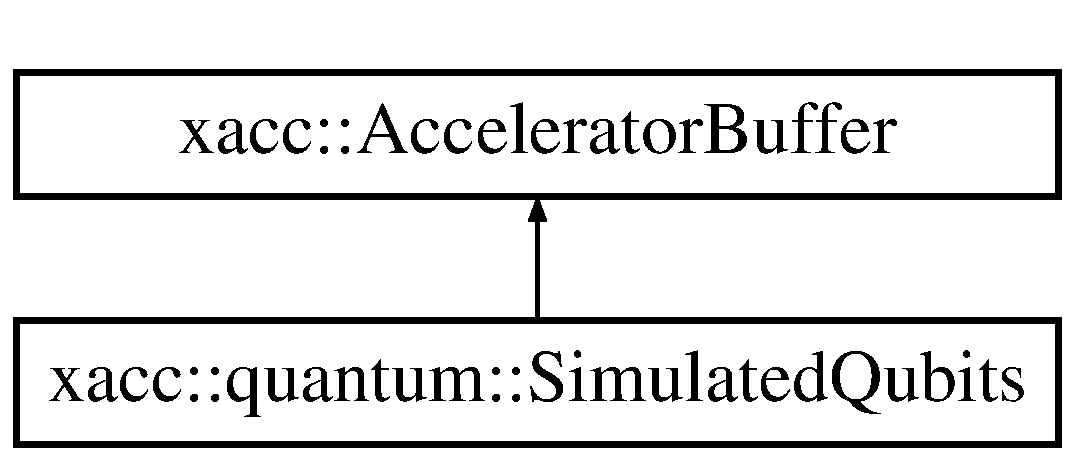
\includegraphics[height=3.000000cm]{a00080}
\end{center}
\end{figure}
\subsection*{Public Member Functions}
\begin{DoxyCompactItemize}
\item 
virtual std\+::shared\+\_\+ptr$<$ \hyperlink{a00167}{xacc\+::\+IR} $>$ \hyperlink{a00080_a0f7f6b10b4a881cb27b36eaa6d39e7b1}{compile} (const std\+::string \&src, std\+::shared\+\_\+ptr$<$ \hyperlink{a00030}{Accelerator} $>$ acc)
\item 
virtual std\+::shared\+\_\+ptr$<$ \hyperlink{a00167}{xacc\+::\+IR} $>$ \hyperlink{a00080_a893e1d1c81a8aaf6e2435c9bceab575e}{compile} (const std\+::string \&src)
\item 
virtual const std\+::string \hyperlink{a00080_a8a180031ae563e1a9aac611e8066c181}{get\+Name} ()
\item 
virtual \hyperlink{a00080_acc0ab28f787b8f4cbeb63c594a247e50}{$\sim$\+D\+Wave\+Compiler} ()
\end{DoxyCompactItemize}
\subsection*{Static Public Member Functions}
\begin{DoxyCompactItemize}
\item 
static void \hyperlink{a00080_a5b221649f22a9bb4d4a304a6522d071f}{register\+Compiler} ()
\end{DoxyCompactItemize}
\subsection*{Additional Inherited Members}


\subsection{Constructor \& Destructor Documentation}
\index{xacc\+::quantum\+::\+D\+Wave\+Compiler@{xacc\+::quantum\+::\+D\+Wave\+Compiler}!````~D\+Wave\+Compiler@{$\sim$\+D\+Wave\+Compiler}}
\index{````~D\+Wave\+Compiler@{$\sim$\+D\+Wave\+Compiler}!xacc\+::quantum\+::\+D\+Wave\+Compiler@{xacc\+::quantum\+::\+D\+Wave\+Compiler}}
\subsubsection[{\texorpdfstring{$\sim$\+D\+Wave\+Compiler()}{~DWaveCompiler()}}]{\setlength{\rightskip}{0pt plus 5cm}virtual xacc\+::quantum\+::\+D\+Wave\+Compiler\+::$\sim$\+D\+Wave\+Compiler (
\begin{DoxyParamCaption}
{}
\end{DoxyParamCaption}
)\hspace{0.3cm}{\ttfamily [inline]}, {\ttfamily [virtual]}}\hypertarget{a00080_acc0ab28f787b8f4cbeb63c594a247e50}{}\label{a00080_acc0ab28f787b8f4cbeb63c594a247e50}
The destructor 

\subsection{Member Function Documentation}
\index{xacc\+::quantum\+::\+D\+Wave\+Compiler@{xacc\+::quantum\+::\+D\+Wave\+Compiler}!compile@{compile}}
\index{compile@{compile}!xacc\+::quantum\+::\+D\+Wave\+Compiler@{xacc\+::quantum\+::\+D\+Wave\+Compiler}}
\subsubsection[{\texorpdfstring{compile(const std\+::string \&src, std\+::shared\+\_\+ptr$<$ Accelerator $>$ acc)}{compile(const std::string \&src, std::shared\_ptr< Accelerator > acc)}}]{\setlength{\rightskip}{0pt plus 5cm}std\+::shared\+\_\+ptr$<$ {\bf IR} $>$ xacc\+::quantum\+::\+D\+Wave\+Compiler\+::compile (
\begin{DoxyParamCaption}
\item[{const std\+::string \&}]{src, }
\item[{std\+::shared\+\_\+ptr$<$ {\bf Accelerator} $>$}]{acc}
\end{DoxyParamCaption}
)\hspace{0.3cm}{\ttfamily [virtual]}}\hypertarget{a00080_a0f7f6b10b4a881cb27b36eaa6d39e7b1}{}\label{a00080_a0f7f6b10b4a881cb27b36eaa6d39e7b1}
This method is to be implemented by derived Compilers and is in charge of executing the compilation mechanism on the provided source string. Implementations also are given access to the \hyperlink{a00030}{Accelerator} that this source code is intended for.


\begin{DoxyParams}{Parameters}
{\em src} & The kernel source string. \\
\hline
{\em acc} & The \hyperlink{a00030}{Accelerator} this code will be executed on \\
\hline
\end{DoxyParams}
\begin{DoxyReturn}{Returns}
ir Intermediate representation for provided source kernel code. 
\end{DoxyReturn}


Implements \hyperlink{a00059_a546a40c95bb93af6a0c0ac48dbeaffc8}{xacc\+::\+Compiler}.

\index{xacc\+::quantum\+::\+D\+Wave\+Compiler@{xacc\+::quantum\+::\+D\+Wave\+Compiler}!compile@{compile}}
\index{compile@{compile}!xacc\+::quantum\+::\+D\+Wave\+Compiler@{xacc\+::quantum\+::\+D\+Wave\+Compiler}}
\subsubsection[{\texorpdfstring{compile(const std\+::string \&src)}{compile(const std::string \&src)}}]{\setlength{\rightskip}{0pt plus 5cm}std\+::shared\+\_\+ptr$<$ {\bf IR} $>$ xacc\+::quantum\+::\+D\+Wave\+Compiler\+::compile (
\begin{DoxyParamCaption}
\item[{const std\+::string \&}]{src}
\end{DoxyParamCaption}
)\hspace{0.3cm}{\ttfamily [virtual]}}\hypertarget{a00080_a893e1d1c81a8aaf6e2435c9bceab575e}{}\label{a00080_a893e1d1c81a8aaf6e2435c9bceab575e}
\begin{DoxyReturn}{Returns}

\end{DoxyReturn}


Implements \hyperlink{a00059_a9092f5f779b570c91569b59621280c04}{xacc\+::\+Compiler}.

\index{xacc\+::quantum\+::\+D\+Wave\+Compiler@{xacc\+::quantum\+::\+D\+Wave\+Compiler}!get\+Name@{get\+Name}}
\index{get\+Name@{get\+Name}!xacc\+::quantum\+::\+D\+Wave\+Compiler@{xacc\+::quantum\+::\+D\+Wave\+Compiler}}
\subsubsection[{\texorpdfstring{get\+Name()}{getName()}}]{\setlength{\rightskip}{0pt plus 5cm}virtual const std\+::string xacc\+::quantum\+::\+D\+Wave\+Compiler\+::get\+Name (
\begin{DoxyParamCaption}
{}
\end{DoxyParamCaption}
)\hspace{0.3cm}{\ttfamily [inline]}, {\ttfamily [virtual]}}\hypertarget{a00080_a8a180031ae563e1a9aac611e8066c181}{}\label{a00080_a8a180031ae563e1a9aac611e8066c181}
Return the name of this \hyperlink{a00059}{Compiler} \begin{DoxyReturn}{Returns}
name \hyperlink{a00059}{Compiler} name 
\end{DoxyReturn}


Implements \hyperlink{a00059_a87fca9100e6462122f5b687c3a0fb3fb}{xacc\+::\+Compiler}.

\index{xacc\+::quantum\+::\+D\+Wave\+Compiler@{xacc\+::quantum\+::\+D\+Wave\+Compiler}!register\+Compiler@{register\+Compiler}}
\index{register\+Compiler@{register\+Compiler}!xacc\+::quantum\+::\+D\+Wave\+Compiler@{xacc\+::quantum\+::\+D\+Wave\+Compiler}}
\subsubsection[{\texorpdfstring{register\+Compiler()}{registerCompiler()}}]{\setlength{\rightskip}{0pt plus 5cm}static void xacc\+::quantum\+::\+D\+Wave\+Compiler\+::register\+Compiler (
\begin{DoxyParamCaption}
{}
\end{DoxyParamCaption}
)\hspace{0.3cm}{\ttfamily [inline]}, {\ttfamily [static]}}\hypertarget{a00080_a5b221649f22a9bb4d4a304a6522d071f}{}\label{a00080_a5b221649f22a9bb4d4a304a6522d071f}
Register this \hyperlink{a00059}{Compiler} with the framework. 

The documentation for this class was generated from the following files\+:\begin{DoxyCompactItemize}
\item 
D\+Wave\+Compiler.\+hpp\item 
D\+Wave\+Compiler.\+cpp\end{DoxyCompactItemize}

\hypertarget{a00081}{}\section{xacc\+:\+:quantum\+:\+:Simulated\+Qubits Class Reference}
\label{a00081}\index{xacc\+::quantum\+::\+Simulated\+Qubits@{xacc\+::quantum\+::\+Simulated\+Qubits}}


{\ttfamily \#include $<$Simulated\+Qubits.\+hpp$>$}

Inheritance diagram for xacc\+:\+:quantum\+:\+:Simulated\+Qubits\+:\begin{figure}[H]
\begin{center}
\leavevmode
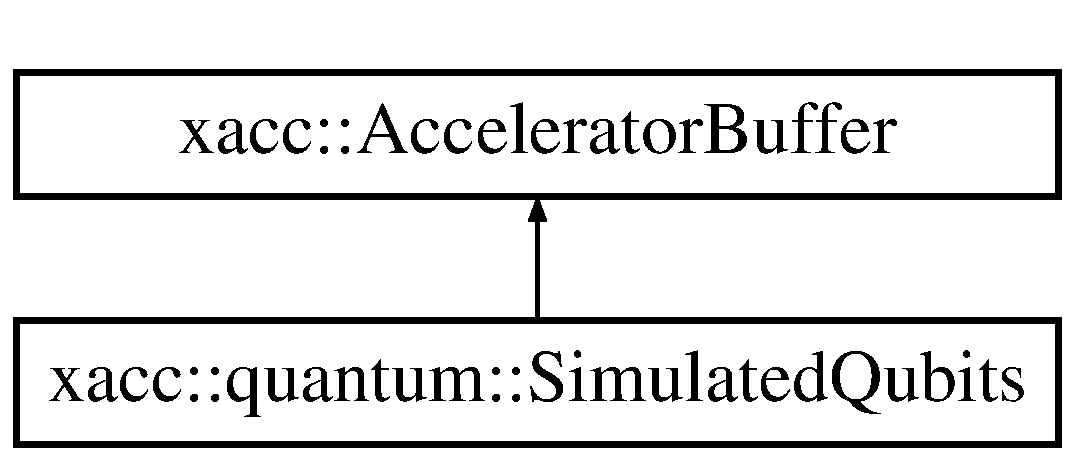
\includegraphics[height=2.000000cm]{a00081}
\end{center}
\end{figure}
\subsection*{Public Member Functions}
\begin{DoxyCompactItemize}
\item 
\hyperlink{a00081_abb0419229628210a1c187b76be6edc30}{Simulated\+Qubits} (const std\+::string \&str, const int N)
\item 
{\footnotesize template$<$typename... Indices$>$ }\\\hyperlink{a00081_ae11d09c17316adb09b93cc866969dba8}{Simulated\+Qubits} (const std\+::string \&str, int first\+Index, Indices...\+indices)
\item 
void \hyperlink{a00081_a3f4518d0135101141bf92d7e31f4fddc}{apply\+Unitary} (fire\+::\+Tensor$<$ 2, fire\+::\+Eigen\+Provider, std\+::complex$<$ double $>$$>$ \&U)
\item 
void \hyperlink{a00081_a09ee499769bb1eedaf08d6b5c29f9791}{normalize} ()
\item 
Qubit\+State \& \hyperlink{a00081_a405577717ca200ed9e524c04209e0216}{get\+State} ()
\item 
void \hyperlink{a00081_a8cd74c239c1fcecb3d03d6989732d5fe}{set\+State} (Qubit\+State \&st)
\item 
virtual void \hyperlink{a00081_a9252d30be0563f36bf1ff839c7104cd7}{print} (std\+::ostream \&stream)
\item 
virtual void \hyperlink{a00081_a32922bd2ccc64bba601c07a3c136cc3d}{print} ()
\item 
virtual \hyperlink{a00081_aebf6f30a6d8c84971091d87908680e7e}{$\sim$\+Simulated\+Qubits} ()
\end{DoxyCompactItemize}
\subsection*{Protected Attributes}
\begin{DoxyCompactItemize}
\item 
Qubit\+State \hyperlink{a00081_a630bea50ee06fd59f74450f01f95e489}{buffer\+State}
\end{DoxyCompactItemize}


\subsection{Detailed Description}
\hyperlink{a00081}{Simulated\+Qubits} is an \hyperlink{a00013}{Accelerator\+Buffer} that models simulated qubits. As such, it keeps track of the state of the qubit buffer using a Rank 1 Fire Tensor.

It provides an interface for applying unitary operations on the qubit buffer state. 

\subsection{Constructor \& Destructor Documentation}
\index{xacc\+::quantum\+::\+Simulated\+Qubits@{xacc\+::quantum\+::\+Simulated\+Qubits}!Simulated\+Qubits@{Simulated\+Qubits}}
\index{Simulated\+Qubits@{Simulated\+Qubits}!xacc\+::quantum\+::\+Simulated\+Qubits@{xacc\+::quantum\+::\+Simulated\+Qubits}}
\subsubsection[{\texorpdfstring{Simulated\+Qubits(const std\+::string \&str, const int N)}{SimulatedQubits(const std::string \&str, const int N)}}]{\setlength{\rightskip}{0pt plus 5cm}xacc\+::quantum\+::\+Simulated\+Qubits\+::\+Simulated\+Qubits (
\begin{DoxyParamCaption}
\item[{const std\+::string \&}]{str, }
\item[{const int}]{N}
\end{DoxyParamCaption}
)\hspace{0.3cm}{\ttfamily [inline]}}\hypertarget{a00081_abb0419229628210a1c187b76be6edc30}{}\label{a00081_abb0419229628210a1c187b76be6edc30}
The Constructor, creates a state with given size N. 
\begin{DoxyParams}{Parameters}
{\em str} & Variable name of this buffer \\
\hline
{\em N} & The number of qubits to model \\
\hline
\end{DoxyParams}
\index{xacc\+::quantum\+::\+Simulated\+Qubits@{xacc\+::quantum\+::\+Simulated\+Qubits}!Simulated\+Qubits@{Simulated\+Qubits}}
\index{Simulated\+Qubits@{Simulated\+Qubits}!xacc\+::quantum\+::\+Simulated\+Qubits@{xacc\+::quantum\+::\+Simulated\+Qubits}}
\subsubsection[{\texorpdfstring{Simulated\+Qubits(const std\+::string \&str, int first\+Index, Indices...\+indices)}{SimulatedQubits(const std::string \&str, int firstIndex, Indices...indices)}}]{\setlength{\rightskip}{0pt plus 5cm}template$<$typename... Indices$>$ xacc\+::quantum\+::\+Simulated\+Qubits\+::\+Simulated\+Qubits (
\begin{DoxyParamCaption}
\item[{const std\+::string \&}]{str, }
\item[{int}]{first\+Index, }
\item[{Indices...}]{indices}
\end{DoxyParamCaption}
)\hspace{0.3cm}{\ttfamily [inline]}}\hypertarget{a00081_ae11d09c17316adb09b93cc866969dba8}{}\label{a00081_ae11d09c17316adb09b93cc866969dba8}
The constructor \index{xacc\+::quantum\+::\+Simulated\+Qubits@{xacc\+::quantum\+::\+Simulated\+Qubits}!````~Simulated\+Qubits@{$\sim$\+Simulated\+Qubits}}
\index{````~Simulated\+Qubits@{$\sim$\+Simulated\+Qubits}!xacc\+::quantum\+::\+Simulated\+Qubits@{xacc\+::quantum\+::\+Simulated\+Qubits}}
\subsubsection[{\texorpdfstring{$\sim$\+Simulated\+Qubits()}{~SimulatedQubits()}}]{\setlength{\rightskip}{0pt plus 5cm}virtual xacc\+::quantum\+::\+Simulated\+Qubits\+::$\sim$\+Simulated\+Qubits (
\begin{DoxyParamCaption}
{}
\end{DoxyParamCaption}
)\hspace{0.3cm}{\ttfamily [inline]}, {\ttfamily [virtual]}}\hypertarget{a00081_aebf6f30a6d8c84971091d87908680e7e}{}\label{a00081_aebf6f30a6d8c84971091d87908680e7e}
The destructor 

\subsection{Member Function Documentation}
\index{xacc\+::quantum\+::\+Simulated\+Qubits@{xacc\+::quantum\+::\+Simulated\+Qubits}!apply\+Unitary@{apply\+Unitary}}
\index{apply\+Unitary@{apply\+Unitary}!xacc\+::quantum\+::\+Simulated\+Qubits@{xacc\+::quantum\+::\+Simulated\+Qubits}}
\subsubsection[{\texorpdfstring{apply\+Unitary(fire\+::\+Tensor$<$ 2, fire\+::\+Eigen\+Provider, std\+::complex$<$ double $>$$>$ \&\+U)}{applyUnitary(fire::Tensor< 2, fire::EigenProvider, std::complex< double >> \&U)}}]{\setlength{\rightskip}{0pt plus 5cm}void xacc\+::quantum\+::\+Simulated\+Qubits\+::apply\+Unitary (
\begin{DoxyParamCaption}
\item[{fire\+::\+Tensor$<$ 2, fire\+::\+Eigen\+Provider, std\+::complex$<$ double $>$$>$ \&}]{U}
\end{DoxyParamCaption}
)\hspace{0.3cm}{\ttfamily [inline]}}\hypertarget{a00081_a3f4518d0135101141bf92d7e31f4fddc}{}\label{a00081_a3f4518d0135101141bf92d7e31f4fddc}
Apply the given unitary matrix to this qubit buffer state.


\begin{DoxyParams}{Parameters}
{\em U} & The unitary matrix to apply to this state \\
\hline
\end{DoxyParams}
\index{xacc\+::quantum\+::\+Simulated\+Qubits@{xacc\+::quantum\+::\+Simulated\+Qubits}!get\+State@{get\+State}}
\index{get\+State@{get\+State}!xacc\+::quantum\+::\+Simulated\+Qubits@{xacc\+::quantum\+::\+Simulated\+Qubits}}
\subsubsection[{\texorpdfstring{get\+State()}{getState()}}]{\setlength{\rightskip}{0pt plus 5cm}Qubit\+State\& xacc\+::quantum\+::\+Simulated\+Qubits\+::get\+State (
\begin{DoxyParamCaption}
{}
\end{DoxyParamCaption}
)\hspace{0.3cm}{\ttfamily [inline]}}\hypertarget{a00081_a405577717ca200ed9e524c04209e0216}{}\label{a00081_a405577717ca200ed9e524c04209e0216}
Return the current state

\begin{DoxyReturn}{Returns}
state This state vector 
\end{DoxyReturn}
\index{xacc\+::quantum\+::\+Simulated\+Qubits@{xacc\+::quantum\+::\+Simulated\+Qubits}!normalize@{normalize}}
\index{normalize@{normalize}!xacc\+::quantum\+::\+Simulated\+Qubits@{xacc\+::quantum\+::\+Simulated\+Qubits}}
\subsubsection[{\texorpdfstring{normalize()}{normalize()}}]{\setlength{\rightskip}{0pt plus 5cm}void xacc\+::quantum\+::\+Simulated\+Qubits\+::normalize (
\begin{DoxyParamCaption}
{}
\end{DoxyParamCaption}
)\hspace{0.3cm}{\ttfamily [inline]}}\hypertarget{a00081_a09ee499769bb1eedaf08d6b5c29f9791}{}\label{a00081_a09ee499769bb1eedaf08d6b5c29f9791}
Normalize the state. \index{xacc\+::quantum\+::\+Simulated\+Qubits@{xacc\+::quantum\+::\+Simulated\+Qubits}!print@{print}}
\index{print@{print}!xacc\+::quantum\+::\+Simulated\+Qubits@{xacc\+::quantum\+::\+Simulated\+Qubits}}
\subsubsection[{\texorpdfstring{print(std\+::ostream \&stream)}{print(std::ostream \&stream)}}]{\setlength{\rightskip}{0pt plus 5cm}virtual void xacc\+::quantum\+::\+Simulated\+Qubits\+::print (
\begin{DoxyParamCaption}
\item[{std\+::ostream \&}]{stream}
\end{DoxyParamCaption}
)\hspace{0.3cm}{\ttfamily [inline]}, {\ttfamily [virtual]}}\hypertarget{a00081_a9252d30be0563f36bf1ff839c7104cd7}{}\label{a00081_a9252d30be0563f36bf1ff839c7104cd7}
Print the state to the provided output stream.


\begin{DoxyParams}{Parameters}
{\em stream} & The output stream to print to \\
\hline
\end{DoxyParams}


Reimplemented from \hyperlink{a00013}{xacc\+::\+Accelerator\+Buffer}.

\index{xacc\+::quantum\+::\+Simulated\+Qubits@{xacc\+::quantum\+::\+Simulated\+Qubits}!print@{print}}
\index{print@{print}!xacc\+::quantum\+::\+Simulated\+Qubits@{xacc\+::quantum\+::\+Simulated\+Qubits}}
\subsubsection[{\texorpdfstring{print()}{print()}}]{\setlength{\rightskip}{0pt plus 5cm}virtual void xacc\+::quantum\+::\+Simulated\+Qubits\+::print (
\begin{DoxyParamCaption}
{}
\end{DoxyParamCaption}
)\hspace{0.3cm}{\ttfamily [inline]}, {\ttfamily [virtual]}}\hypertarget{a00081_a32922bd2ccc64bba601c07a3c136cc3d}{}\label{a00081_a32922bd2ccc64bba601c07a3c136cc3d}
Print to X\+A\+CC Info 

Reimplemented from \hyperlink{a00013}{xacc\+::\+Accelerator\+Buffer}.

\index{xacc\+::quantum\+::\+Simulated\+Qubits@{xacc\+::quantum\+::\+Simulated\+Qubits}!set\+State@{set\+State}}
\index{set\+State@{set\+State}!xacc\+::quantum\+::\+Simulated\+Qubits@{xacc\+::quantum\+::\+Simulated\+Qubits}}
\subsubsection[{\texorpdfstring{set\+State(\+Qubit\+State \&st)}{setState(QubitState \&st)}}]{\setlength{\rightskip}{0pt plus 5cm}void xacc\+::quantum\+::\+Simulated\+Qubits\+::set\+State (
\begin{DoxyParamCaption}
\item[{Qubit\+State \&}]{st}
\end{DoxyParamCaption}
)\hspace{0.3cm}{\ttfamily [inline]}}\hypertarget{a00081_a8cd74c239c1fcecb3d03d6989732d5fe}{}\label{a00081_a8cd74c239c1fcecb3d03d6989732d5fe}
Set the state. 
\begin{DoxyParams}{Parameters}
{\em st} & The state to set on this buffer. \\
\hline
\end{DoxyParams}


\subsection{Member Data Documentation}
\index{xacc\+::quantum\+::\+Simulated\+Qubits@{xacc\+::quantum\+::\+Simulated\+Qubits}!buffer\+State@{buffer\+State}}
\index{buffer\+State@{buffer\+State}!xacc\+::quantum\+::\+Simulated\+Qubits@{xacc\+::quantum\+::\+Simulated\+Qubits}}
\subsubsection[{\texorpdfstring{buffer\+State}{bufferState}}]{\setlength{\rightskip}{0pt plus 5cm}Qubit\+State xacc\+::quantum\+::\+Simulated\+Qubits\+::buffer\+State\hspace{0.3cm}{\ttfamily [protected]}}\hypertarget{a00081_a630bea50ee06fd59f74450f01f95e489}{}\label{a00081_a630bea50ee06fd59f74450f01f95e489}
The qubit buffer state. 

The documentation for this class was generated from the following file\+:\begin{DoxyCompactItemize}
\item 
Simulated\+Qubits.\+hpp\end{DoxyCompactItemize}

\hypertarget{a00082}{}\section{xacc\+:\+:Singleton$<$ T $>$ Class Template Reference}
\label{a00082}\index{xacc\+::\+Singleton$<$ T $>$@{xacc\+::\+Singleton$<$ T $>$}}


{\ttfamily \#include $<$Singleton.\+hpp$>$}

\subsection*{Static Public Member Functions}
\begin{DoxyCompactItemize}
\item 
static T $\ast$ \hyperlink{a00082_ae4c30f303439e702389c9d088abb3f23}{instance} ()
\item 
static void \hyperlink{a00082_abbc654f5f90a2abc85f0010496335942}{destroy} ()
\end{DoxyCompactItemize}
\subsection*{Protected Member Functions}
\begin{DoxyCompactItemize}
\item 
\hyperlink{a00082_afd62caabc41babdd98ab9af2253ec371}{Singleton} ()
\item 
virtual \hyperlink{a00082_a75a032ec71f88d6986461b47f3fb2600}{$\sim$\+Singleton} ()
\end{DoxyCompactItemize}
\subsection*{Static Protected Attributes}
\begin{DoxyCompactItemize}
\item 
static T $\ast$ \hyperlink{a00082_a863885efab9990f06f699567648dfa26}{instance\+\_\+} = nullptr
\end{DoxyCompactItemize}


\subsection{Detailed Description}
\subsubsection*{template$<$class T$>$\\*
class xacc\+::\+Singleton$<$ T $>$}

\hyperlink{a00082}{Singleton} provides a templated implementation of the \hyperlink{a00082}{Singleton} Design Pattern. This class takes a template parameter and provides behviour around that template that models a singleton -\/ ie there is only one instance available during runtime. 

\subsection{Constructor \& Destructor Documentation}
\index{xacc\+::\+Singleton@{xacc\+::\+Singleton}!Singleton@{Singleton}}
\index{Singleton@{Singleton}!xacc\+::\+Singleton@{xacc\+::\+Singleton}}
\subsubsection[{\texorpdfstring{Singleton()}{Singleton()}}]{\setlength{\rightskip}{0pt plus 5cm}template$<$class T$>$ {\bf xacc\+::\+Singleton}$<$ T $>$\+::{\bf Singleton} (
\begin{DoxyParamCaption}
{}
\end{DoxyParamCaption}
)\hspace{0.3cm}{\ttfamily [inline]}, {\ttfamily [explicit]}, {\ttfamily [protected]}}\hypertarget{a00082_afd62caabc41babdd98ab9af2253ec371}{}\label{a00082_afd62caabc41babdd98ab9af2253ec371}
constructor \index{xacc\+::\+Singleton@{xacc\+::\+Singleton}!````~Singleton@{$\sim$\+Singleton}}
\index{````~Singleton@{$\sim$\+Singleton}!xacc\+::\+Singleton@{xacc\+::\+Singleton}}
\subsubsection[{\texorpdfstring{$\sim$\+Singleton()}{~Singleton()}}]{\setlength{\rightskip}{0pt plus 5cm}template$<$class T$>$ virtual {\bf xacc\+::\+Singleton}$<$ T $>$\+::$\sim${\bf Singleton} (
\begin{DoxyParamCaption}
{}
\end{DoxyParamCaption}
)\hspace{0.3cm}{\ttfamily [inline]}, {\ttfamily [protected]}, {\ttfamily [virtual]}}\hypertarget{a00082_a75a032ec71f88d6986461b47f3fb2600}{}\label{a00082_a75a032ec71f88d6986461b47f3fb2600}
destructor 

\subsection{Member Function Documentation}
\index{xacc\+::\+Singleton@{xacc\+::\+Singleton}!destroy@{destroy}}
\index{destroy@{destroy}!xacc\+::\+Singleton@{xacc\+::\+Singleton}}
\subsubsection[{\texorpdfstring{destroy()}{destroy()}}]{\setlength{\rightskip}{0pt plus 5cm}template$<$class T$>$ static void {\bf xacc\+::\+Singleton}$<$ T $>$\+::destroy (
\begin{DoxyParamCaption}
{}
\end{DoxyParamCaption}
)\hspace{0.3cm}{\ttfamily [inline]}, {\ttfamily [static]}}\hypertarget{a00082_abbc654f5f90a2abc85f0010496335942}{}\label{a00082_abbc654f5f90a2abc85f0010496335942}
Destroy the single instance of T \index{xacc\+::\+Singleton@{xacc\+::\+Singleton}!instance@{instance}}
\index{instance@{instance}!xacc\+::\+Singleton@{xacc\+::\+Singleton}}
\subsubsection[{\texorpdfstring{instance()}{instance()}}]{\setlength{\rightskip}{0pt plus 5cm}template$<$class T$>$ static T$\ast$ {\bf xacc\+::\+Singleton}$<$ T $>$\+::instance (
\begin{DoxyParamCaption}
{}
\end{DoxyParamCaption}
)\hspace{0.3cm}{\ttfamily [inline]}, {\ttfamily [static]}}\hypertarget{a00082_ae4c30f303439e702389c9d088abb3f23}{}\label{a00082_ae4c30f303439e702389c9d088abb3f23}
Return the single instance of T \begin{DoxyReturn}{Returns}
instance The singleton instance 
\end{DoxyReturn}


\subsection{Member Data Documentation}
\index{xacc\+::\+Singleton@{xacc\+::\+Singleton}!instance\+\_\+@{instance\+\_\+}}
\index{instance\+\_\+@{instance\+\_\+}!xacc\+::\+Singleton@{xacc\+::\+Singleton}}
\subsubsection[{\texorpdfstring{instance\+\_\+}{instance\_}}]{\setlength{\rightskip}{0pt plus 5cm}template$<$class T$>$ T $\ast$ {\bf xacc\+::\+Singleton}$<$ T $>$\+::instance\+\_\+ = nullptr\hspace{0.3cm}{\ttfamily [static]}, {\ttfamily [protected]}}\hypertarget{a00082_a863885efab9990f06f699567648dfa26}{}\label{a00082_a863885efab9990f06f699567648dfa26}
Reference to the single T instance 

The documentation for this class was generated from the following file\+:\begin{DoxyCompactItemize}
\item 
Singleton.\+hpp\end{DoxyCompactItemize}

\hypertarget{a00083}{}\section{xacc\+:\+:quantum\+:\+:Swap Class Reference}
\label{a00083}\index{xacc\+::quantum\+::\+Swap@{xacc\+::quantum\+::\+Swap}}
Inheritance diagram for xacc\+:\+:quantum\+:\+:Swap\+:\begin{figure}[H]
\begin{center}
\leavevmode
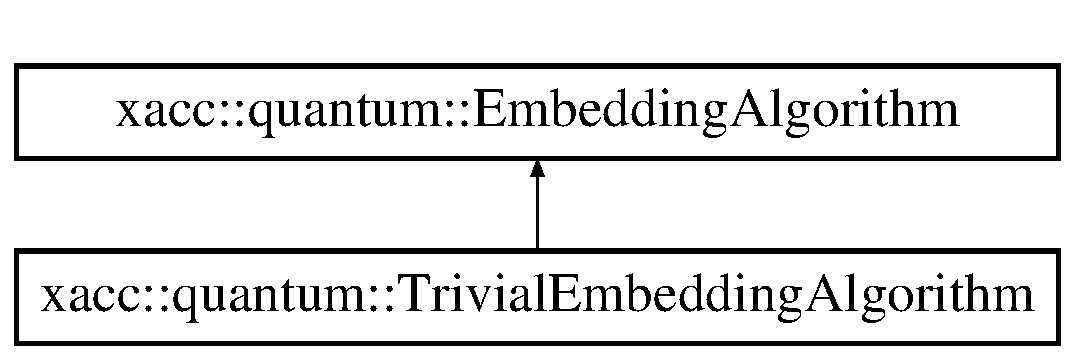
\includegraphics[height=4.000000cm]{a00083}
\end{center}
\end{figure}
\subsection*{Public Member Functions}
\begin{DoxyCompactItemize}
\item 
{\bfseries Swap} (std\+::vector$<$ int $>$ \hyperlink{a00042_a2a56be6c2519ea65df4d06f4abae1393}{qbits})\hypertarget{a00083_a5c35a23a635f235a5615be65e769c121}{}\label{a00083_a5c35a23a635f235a5615be65e769c121}

\item 
{\bfseries Swap} (int control\+Qubit, int target\+Qubit)\hypertarget{a00083_ac19efe303b798e14441a2c235b5ba7f3}{}\label{a00083_ac19efe303b798e14441a2c235b5ba7f3}

\end{DoxyCompactItemize}
\subsection*{Additional Inherited Members}


The documentation for this class was generated from the following files\+:\begin{DoxyCompactItemize}
\item 
Swap.\+hpp\item 
Swap.\+cpp\end{DoxyCompactItemize}

\hypertarget{a00084}{}\section{fire\+:\+:Eigen\+Tensor\+Provider$<$ Rank, Scalar $>$ Class Template Reference}
\label{a00084}\index{fire\+::\+Eigen\+Tensor\+Provider$<$ Rank, Scalar $>$@{fire\+::\+Eigen\+Tensor\+Provider$<$ Rank, Scalar $>$}}


{\ttfamily \#include $<$Eigen\+Tensor\+Provider.\+hpp$>$}

Inheritance diagram for fire\+:\+:Eigen\+Tensor\+Provider$<$ Rank, Scalar $>$\+:\begin{figure}[H]
\begin{center}
\leavevmode
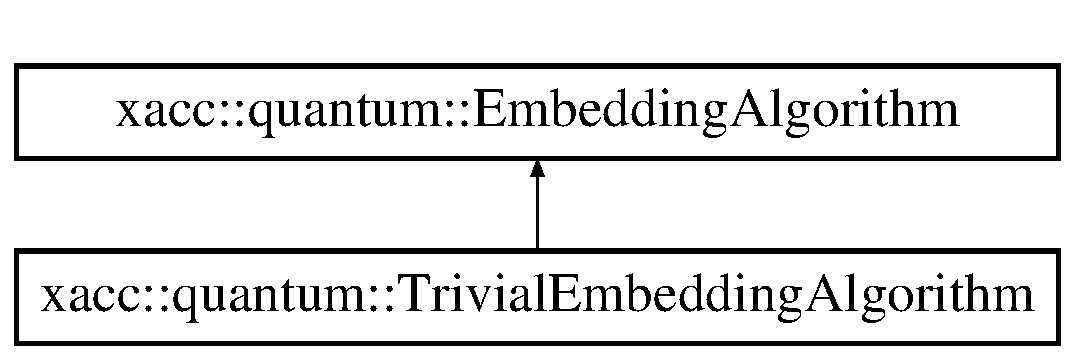
\includegraphics[height=2.000000cm]{a00084}
\end{center}
\end{figure}
\subsection*{Public Member Functions}
\begin{DoxyCompactItemize}
\item 
\hyperlink{a00084_a666937cbdec96978bdd47132a95ab9e6}{Eigen\+Tensor\+Provider} ()
\item 
{\footnotesize template$<$typename... Dimensions$>$ }\\void \hyperlink{a00084_a2d624402c063c0398f018417aae2fe28}{initialize\+Tensor\+Backend} (int first\+Dim, Dimensions...\+other\+Dims)
\item 
void \hyperlink{a00084_a284d6bb6a8539c5776e00d2a377d188e}{initialize\+Tensor\+Backend\+With\+Reference} (\hyperlink{a00822_a1bf491fd1c876e2808648b2fd291e3dd}{Tensor\+Reference}$<$ Scalar $>$ \&reference)
\item 
{\footnotesize template$<$typename... Indices$>$ }\\Scalar \& \hyperlink{a00084_abc61cda0193bc5f5d7fcf17ff8e96d82}{tensor\+Coefficient} (Indices...\+indices)
\item 
bool \hyperlink{a00084_a3e15190363627f4c6b373dc56dd2b4f3}{check\+Equality} (\hyperlink{a00822_a1bf491fd1c876e2808648b2fd291e3dd}{Tensor\+Reference}$<$ Scalar $>$ \&other)
\item 
{\footnotesize template$<$typename Other\+Derived , typename Contraction\+Dims $>$ }\\\hyperlink{a00822_a1bf491fd1c876e2808648b2fd291e3dd}{Tensor\+Reference}$<$ Scalar $>$ \hyperlink{a00084_acd9f39dacb5fd6c35f3f840ed22194e9}{execute\+Contraction} (Other\+Derived \&t2, Contraction\+Dims \&c\+Indices)
\item 
Scalar $\ast$ \hyperlink{a00084_aff5626be9e55f593f0a6b71174ecbd8a}{data} ()
\item 
\hyperlink{a00822_a1bf491fd1c876e2808648b2fd291e3dd}{Tensor\+Reference}$<$ Scalar $>$ \hyperlink{a00084_a957d54e0259b1ea798a47389af4b8379}{add} (\hyperlink{a00822_a1bf491fd1c876e2808648b2fd291e3dd}{Tensor\+Reference}$<$ Scalar $>$ \&other)
\item 
{\footnotesize template$<$typename Init\+List $>$ }\\void \hyperlink{a00084_a3d02dbf7e2d255a1378084aa6459cf25}{set\+Tensor\+Values} (Init\+List \&vals)
\item 
void \hyperlink{a00084_a607ad28d9f0b8b7f639dc1b0693dfd03}{print\+Tensor} (std\+::ostream \&stream)
\item 
void \hyperlink{a00084_a461c3348c66ae011167d8c194c79dce9}{fill\+With\+Random\+Values} ()
\item 
\hyperlink{a00822_a1bf491fd1c876e2808648b2fd291e3dd}{Tensor\+Reference}$<$ Scalar $>$ \hyperlink{a00084_ae526f2376663adc8788ba8f4c04eb6cb}{scalar\+Product} (Scalar \&val)
\item 
{\footnotesize template$<$typename Dim\+Array $>$ }\\\hyperlink{a00822_a1bf491fd1c876e2808648b2fd291e3dd}{Tensor\+Reference}$<$ Scalar $>$ \hyperlink{a00084_a5ffd64a2a2a7b5886b2175d21a46dccf}{reshape\+Tensor} (Dim\+Array \&array)
\item 
{\footnotesize template$<$typename Dim\+Array $>$ }\\\hyperlink{a00822_a1bf491fd1c876e2808648b2fd291e3dd}{Tensor\+Reference}$<$ Scalar $>$ {\bfseries shuffle\+Tensor} (Dim\+Array \&array)\hypertarget{a00084_ac4d85c2ce0bfb666ddb7284241b74dcb}{}\label{a00084_ac4d85c2ce0bfb666ddb7284241b74dcb}

\item 
std\+::tuple$<$ \hyperlink{a00822_a1bf491fd1c876e2808648b2fd291e3dd}{Tensor\+Reference}$<$ Scalar $>$, \hyperlink{a00822_a1bf491fd1c876e2808648b2fd291e3dd}{Tensor\+Reference}$<$ Scalar $>$, \hyperlink{a00822_a1bf491fd1c876e2808648b2fd291e3dd}{Tensor\+Reference}$<$ Scalar $>$ $>$ {\bfseries compute\+Svd} (\hyperlink{a00822_a1bf491fd1c876e2808648b2fd291e3dd}{Tensor\+Reference}$<$ Scalar $>$ \&ref, double cutoff)\hypertarget{a00084_aa1ba881990a0af6e0a68f8927f94c89d}{}\label{a00084_aa1ba881990a0af6e0a68f8927f94c89d}

\item 
\hyperlink{a00822_a1bf491fd1c876e2808648b2fd291e3dd}{Tensor\+Reference}$<$ Scalar $>$ {\bfseries kron\+Prod} (\hyperlink{a00822_a1bf491fd1c876e2808648b2fd291e3dd}{Tensor\+Reference}$<$ Scalar $>$ \&other)\hypertarget{a00084_ade4eea42a36aaa42cb8ea85ae3dee711}{}\label{a00084_ade4eea42a36aaa42cb8ea85ae3dee711}

\end{DoxyCompactItemize}
\subsection*{Static Public Member Functions}
\begin{DoxyCompactItemize}
\item 
static constexpr int \hyperlink{a00084_a68f0ad7ead91dec2ea56f173981465c8}{get\+Rank} ()
\end{DoxyCompactItemize}
\subsection*{Static Public Attributes}
\begin{DoxyCompactItemize}
\item 
static const int \hyperlink{a00084_ae8f0217985d78dba31d7bdb95ace1e43}{rank} = Rank
\end{DoxyCompactItemize}


\subsection{Detailed Description}
\subsubsection*{template$<$const int Rank, typename Scalar = double$>$\\*
class fire\+::\+Eigen\+Tensor\+Provider$<$ Rank, Scalar $>$}

The \hyperlink{a00084}{Eigen\+Tensor\+Provider} is a \hyperlink{a00300}{Tensor\+Provider} that provides tensor data and operations using the Eigen C++ tensor module. 

\subsection{Constructor \& Destructor Documentation}
\index{fire\+::\+Eigen\+Tensor\+Provider@{fire\+::\+Eigen\+Tensor\+Provider}!Eigen\+Tensor\+Provider@{Eigen\+Tensor\+Provider}}
\index{Eigen\+Tensor\+Provider@{Eigen\+Tensor\+Provider}!fire\+::\+Eigen\+Tensor\+Provider@{fire\+::\+Eigen\+Tensor\+Provider}}
\subsubsection[{\texorpdfstring{Eigen\+Tensor\+Provider()}{EigenTensorProvider()}}]{\setlength{\rightskip}{0pt plus 5cm}template$<$const int Rank, typename Scalar = double$>$ {\bf fire\+::\+Eigen\+Tensor\+Provider}$<$ Rank, Scalar $>$\+::{\bf Eigen\+Tensor\+Provider} (
\begin{DoxyParamCaption}
{}
\end{DoxyParamCaption}
)\hspace{0.3cm}{\ttfamily [inline]}}\hypertarget{a00084_a666937cbdec96978bdd47132a95ab9e6}{}\label{a00084_a666937cbdec96978bdd47132a95ab9e6}
The Constructor 

\subsection{Member Function Documentation}
\index{fire\+::\+Eigen\+Tensor\+Provider@{fire\+::\+Eigen\+Tensor\+Provider}!add@{add}}
\index{add@{add}!fire\+::\+Eigen\+Tensor\+Provider@{fire\+::\+Eigen\+Tensor\+Provider}}
\subsubsection[{\texorpdfstring{add(\+Tensor\+Reference$<$ Scalar $>$ \&other)}{add(TensorReference< Scalar > \&other)}}]{\setlength{\rightskip}{0pt plus 5cm}template$<$const int Rank, typename Scalar = double$>$ {\bf Tensor\+Reference}$<$Scalar$>$ {\bf fire\+::\+Eigen\+Tensor\+Provider}$<$ Rank, Scalar $>$\+::add (
\begin{DoxyParamCaption}
\item[{{\bf Tensor\+Reference}$<$ Scalar $>$ \&}]{other}
\end{DoxyParamCaption}
)\hspace{0.3cm}{\ttfamily [inline]}}\hypertarget{a00084_a957d54e0259b1ea798a47389af4b8379}{}\label{a00084_a957d54e0259b1ea798a47389af4b8379}
Return a Tensor\+Reference representing the sum of this Eigen \hyperlink{a00299}{Tensor} and an Eigen \hyperlink{a00299}{Tensor} represented by the other Tensor\+Reference.


\begin{DoxyParams}{Parameters}
{\em other} & Tensor\+Reference view of the other \hyperlink{a00299}{Tensor} \\
\hline
\end{DoxyParams}
\begin{DoxyReturn}{Returns}
result A new Tensor\+Reference representing the sum of this and other. 
\end{DoxyReturn}
\index{fire\+::\+Eigen\+Tensor\+Provider@{fire\+::\+Eigen\+Tensor\+Provider}!check\+Equality@{check\+Equality}}
\index{check\+Equality@{check\+Equality}!fire\+::\+Eigen\+Tensor\+Provider@{fire\+::\+Eigen\+Tensor\+Provider}}
\subsubsection[{\texorpdfstring{check\+Equality(\+Tensor\+Reference$<$ Scalar $>$ \&other)}{checkEquality(TensorReference< Scalar > \&other)}}]{\setlength{\rightskip}{0pt plus 5cm}template$<$const int Rank, typename Scalar = double$>$ bool {\bf fire\+::\+Eigen\+Tensor\+Provider}$<$ Rank, Scalar $>$\+::check\+Equality (
\begin{DoxyParamCaption}
\item[{{\bf Tensor\+Reference}$<$ Scalar $>$ \&}]{other}
\end{DoxyParamCaption}
)\hspace{0.3cm}{\ttfamily [inline]}}\hypertarget{a00084_a3e15190363627f4c6b373dc56dd2b4f3}{}\label{a00084_a3e15190363627f4c6b373dc56dd2b4f3}
Return true if the provided Tensor\+Reference as a tensor is equal to this tensor.


\begin{DoxyParams}{Parameters}
{\em other} & Tensor\+Reference view of the other \hyperlink{a00299}{Tensor} \\
\hline
\end{DoxyParams}
\begin{DoxyReturn}{Returns}
equal A boolean indicating if these Tensors are equal 
\end{DoxyReturn}
\index{fire\+::\+Eigen\+Tensor\+Provider@{fire\+::\+Eigen\+Tensor\+Provider}!data@{data}}
\index{data@{data}!fire\+::\+Eigen\+Tensor\+Provider@{fire\+::\+Eigen\+Tensor\+Provider}}
\subsubsection[{\texorpdfstring{data()}{data()}}]{\setlength{\rightskip}{0pt plus 5cm}template$<$const int Rank, typename Scalar = double$>$ Scalar$\ast$ {\bf fire\+::\+Eigen\+Tensor\+Provider}$<$ Rank, Scalar $>$\+::data (
\begin{DoxyParamCaption}
{}
\end{DoxyParamCaption}
)\hspace{0.3cm}{\ttfamily [inline]}}\hypertarget{a00084_aff5626be9e55f593f0a6b71174ecbd8a}{}\label{a00084_aff5626be9e55f593f0a6b71174ecbd8a}
Return the 1-\/D array wrapped by this Eigen \hyperlink{a00299}{Tensor}

\begin{DoxyReturn}{Returns}
data 1-\/D array of data representing the tensor in this \hyperlink{a00300}{Tensor\+Provider} 
\end{DoxyReturn}
\index{fire\+::\+Eigen\+Tensor\+Provider@{fire\+::\+Eigen\+Tensor\+Provider}!execute\+Contraction@{execute\+Contraction}}
\index{execute\+Contraction@{execute\+Contraction}!fire\+::\+Eigen\+Tensor\+Provider@{fire\+::\+Eigen\+Tensor\+Provider}}
\subsubsection[{\texorpdfstring{execute\+Contraction(\+Other\+Derived \&t2, Contraction\+Dims \&c\+Indices)}{executeContraction(OtherDerived \&t2, ContractionDims \&cIndices)}}]{\setlength{\rightskip}{0pt plus 5cm}template$<$const int Rank, typename Scalar = double$>$ template$<$typename Other\+Derived , typename Contraction\+Dims $>$ {\bf Tensor\+Reference}$<$Scalar$>$ {\bf fire\+::\+Eigen\+Tensor\+Provider}$<$ Rank, Scalar $>$\+::execute\+Contraction (
\begin{DoxyParamCaption}
\item[{Other\+Derived \&}]{t2, }
\item[{Contraction\+Dims \&}]{c\+Indices}
\end{DoxyParamCaption}
)\hspace{0.3cm}{\ttfamily [inline]}}\hypertarget{a00084_acd9f39dacb5fd6c35f3f840ed22194e9}{}\label{a00084_acd9f39dacb5fd6c35f3f840ed22194e9}
Compute the tensor contraction of this Eigen \hyperlink{a00299}{Tensor} with the provided Other \hyperlink{a00299}{Tensor}.


\begin{DoxyParams}{Parameters}
{\em t2} & The other \hyperlink{a00299}{Tensor} \\
\hline
{\em indices} & The contraction indices. \\
\hline
\end{DoxyParams}
\begin{DoxyReturn}{Returns}
result The contraction result as a Tensor\+Reference 
\end{DoxyReturn}
\index{fire\+::\+Eigen\+Tensor\+Provider@{fire\+::\+Eigen\+Tensor\+Provider}!fill\+With\+Random\+Values@{fill\+With\+Random\+Values}}
\index{fill\+With\+Random\+Values@{fill\+With\+Random\+Values}!fire\+::\+Eigen\+Tensor\+Provider@{fire\+::\+Eigen\+Tensor\+Provider}}
\subsubsection[{\texorpdfstring{fill\+With\+Random\+Values()}{fillWithRandomValues()}}]{\setlength{\rightskip}{0pt plus 5cm}template$<$const int Rank, typename Scalar = double$>$ void {\bf fire\+::\+Eigen\+Tensor\+Provider}$<$ Rank, Scalar $>$\+::fill\+With\+Random\+Values (
\begin{DoxyParamCaption}
{}
\end{DoxyParamCaption}
)\hspace{0.3cm}{\ttfamily [inline]}}\hypertarget{a00084_a461c3348c66ae011167d8c194c79dce9}{}\label{a00084_a461c3348c66ae011167d8c194c79dce9}
Set the Eigen \hyperlink{a00299}{Tensor} values to random values. \index{fire\+::\+Eigen\+Tensor\+Provider@{fire\+::\+Eigen\+Tensor\+Provider}!get\+Rank@{get\+Rank}}
\index{get\+Rank@{get\+Rank}!fire\+::\+Eigen\+Tensor\+Provider@{fire\+::\+Eigen\+Tensor\+Provider}}
\subsubsection[{\texorpdfstring{get\+Rank()}{getRank()}}]{\setlength{\rightskip}{0pt plus 5cm}template$<$const int Rank, typename Scalar = double$>$ static constexpr int {\bf fire\+::\+Eigen\+Tensor\+Provider}$<$ Rank, Scalar $>$\+::get\+Rank (
\begin{DoxyParamCaption}
{}
\end{DoxyParamCaption}
)\hspace{0.3cm}{\ttfamily [inline]}, {\ttfamily [static]}}\hypertarget{a00084_a68f0ad7ead91dec2ea56f173981465c8}{}\label{a00084_a68f0ad7ead91dec2ea56f173981465c8}
Return the rank of this Eigen \hyperlink{a00299}{Tensor}

\begin{DoxyReturn}{Returns}
rank The rank of this \hyperlink{a00299}{Tensor} 
\end{DoxyReturn}
\index{fire\+::\+Eigen\+Tensor\+Provider@{fire\+::\+Eigen\+Tensor\+Provider}!initialize\+Tensor\+Backend@{initialize\+Tensor\+Backend}}
\index{initialize\+Tensor\+Backend@{initialize\+Tensor\+Backend}!fire\+::\+Eigen\+Tensor\+Provider@{fire\+::\+Eigen\+Tensor\+Provider}}
\subsubsection[{\texorpdfstring{initialize\+Tensor\+Backend(int first\+Dim, Dimensions...\+other\+Dims)}{initializeTensorBackend(int firstDim, Dimensions...otherDims)}}]{\setlength{\rightskip}{0pt plus 5cm}template$<$const int Rank, typename Scalar = double$>$ template$<$typename... Dimensions$>$ void {\bf fire\+::\+Eigen\+Tensor\+Provider}$<$ Rank, Scalar $>$\+::initialize\+Tensor\+Backend (
\begin{DoxyParamCaption}
\item[{int}]{first\+Dim, }
\item[{Dimensions...}]{other\+Dims}
\end{DoxyParamCaption}
)\hspace{0.3cm}{\ttfamily [inline]}}\hypertarget{a00084_a2d624402c063c0398f018417aae2fe28}{}\label{a00084_a2d624402c063c0398f018417aae2fe28}
Initialize the Eigen \hyperlink{a00299}{Tensor} with all zeros. 
\begin{DoxyParams}{Parameters}
{\em first\+Dim} & \\
\hline
{\em other\+Dims} & \\
\hline
\end{DoxyParams}
\index{fire\+::\+Eigen\+Tensor\+Provider@{fire\+::\+Eigen\+Tensor\+Provider}!initialize\+Tensor\+Backend\+With\+Reference@{initialize\+Tensor\+Backend\+With\+Reference}}
\index{initialize\+Tensor\+Backend\+With\+Reference@{initialize\+Tensor\+Backend\+With\+Reference}!fire\+::\+Eigen\+Tensor\+Provider@{fire\+::\+Eigen\+Tensor\+Provider}}
\subsubsection[{\texorpdfstring{initialize\+Tensor\+Backend\+With\+Reference(\+Tensor\+Reference$<$ Scalar $>$ \&reference)}{initializeTensorBackendWithReference(TensorReference< Scalar > \&reference)}}]{\setlength{\rightskip}{0pt plus 5cm}template$<$const int Rank, typename Scalar = double$>$ void {\bf fire\+::\+Eigen\+Tensor\+Provider}$<$ Rank, Scalar $>$\+::initialize\+Tensor\+Backend\+With\+Reference (
\begin{DoxyParamCaption}
\item[{{\bf Tensor\+Reference}$<$ Scalar $>$ \&}]{reference}
\end{DoxyParamCaption}
)\hspace{0.3cm}{\ttfamily [inline]}}\hypertarget{a00084_a284d6bb6a8539c5776e00d2a377d188e}{}\label{a00084_a284d6bb6a8539c5776e00d2a377d188e}
Initialize the Eigen \hyperlink{a00299}{Tensor} from an existing Tensor\+Reference 
\begin{DoxyParams}{Parameters}
{\em reference} & \\
\hline
\end{DoxyParams}
\index{fire\+::\+Eigen\+Tensor\+Provider@{fire\+::\+Eigen\+Tensor\+Provider}!print\+Tensor@{print\+Tensor}}
\index{print\+Tensor@{print\+Tensor}!fire\+::\+Eigen\+Tensor\+Provider@{fire\+::\+Eigen\+Tensor\+Provider}}
\subsubsection[{\texorpdfstring{print\+Tensor(std\+::ostream \&stream)}{printTensor(std::ostream \&stream)}}]{\setlength{\rightskip}{0pt plus 5cm}template$<$const int Rank, typename Scalar = double$>$ void {\bf fire\+::\+Eigen\+Tensor\+Provider}$<$ Rank, Scalar $>$\+::print\+Tensor (
\begin{DoxyParamCaption}
\item[{std\+::ostream \&}]{stream}
\end{DoxyParamCaption}
)\hspace{0.3cm}{\ttfamily [inline]}}\hypertarget{a00084_a607ad28d9f0b8b7f639dc1b0693dfd03}{}\label{a00084_a607ad28d9f0b8b7f639dc1b0693dfd03}
Output this Eigen \hyperlink{a00299}{Tensor} to the provided output stream.


\begin{DoxyParams}{Parameters}
{\em output\+Stream} & The output stream to write the tensor to. \\
\hline
\end{DoxyParams}
\index{fire\+::\+Eigen\+Tensor\+Provider@{fire\+::\+Eigen\+Tensor\+Provider}!reshape\+Tensor@{reshape\+Tensor}}
\index{reshape\+Tensor@{reshape\+Tensor}!fire\+::\+Eigen\+Tensor\+Provider@{fire\+::\+Eigen\+Tensor\+Provider}}
\subsubsection[{\texorpdfstring{reshape\+Tensor(\+Dim\+Array \&array)}{reshapeTensor(DimArray \&array)}}]{\setlength{\rightskip}{0pt plus 5cm}template$<$const int Rank, typename Scalar = double$>$ template$<$typename Dim\+Array $>$ {\bf Tensor\+Reference}$<$Scalar$>$ {\bf fire\+::\+Eigen\+Tensor\+Provider}$<$ Rank, Scalar $>$\+::reshape\+Tensor (
\begin{DoxyParamCaption}
\item[{Dim\+Array \&}]{array}
\end{DoxyParamCaption}
)\hspace{0.3cm}{\ttfamily [inline]}}\hypertarget{a00084_a5ffd64a2a2a7b5886b2175d21a46dccf}{}\label{a00084_a5ffd64a2a2a7b5886b2175d21a46dccf}
Reshape the Eigen \hyperlink{a00299}{Tensor} with a new array of dimensions


\begin{DoxyParams}{Parameters}
{\em array} & Array of new dimensions for each rank index \\
\hline
\end{DoxyParams}
\begin{DoxyReturn}{Returns}
reshaped\+Tensor A Tensor\+Reference representing new reshaped tensor. 
\end{DoxyReturn}
\index{fire\+::\+Eigen\+Tensor\+Provider@{fire\+::\+Eigen\+Tensor\+Provider}!scalar\+Product@{scalar\+Product}}
\index{scalar\+Product@{scalar\+Product}!fire\+::\+Eigen\+Tensor\+Provider@{fire\+::\+Eigen\+Tensor\+Provider}}
\subsubsection[{\texorpdfstring{scalar\+Product(\+Scalar \&val)}{scalarProduct(Scalar \&val)}}]{\setlength{\rightskip}{0pt plus 5cm}template$<$const int Rank, typename Scalar = double$>$ {\bf Tensor\+Reference}$<$Scalar$>$ {\bf fire\+::\+Eigen\+Tensor\+Provider}$<$ Rank, Scalar $>$\+::scalar\+Product (
\begin{DoxyParamCaption}
\item[{Scalar \&}]{val}
\end{DoxyParamCaption}
)\hspace{0.3cm}{\ttfamily [inline]}}\hypertarget{a00084_ae526f2376663adc8788ba8f4c04eb6cb}{}\label{a00084_ae526f2376663adc8788ba8f4c04eb6cb}
Multiply all elements of this Eigen \hyperlink{a00299}{Tensor} by the provided Scalar.


\begin{DoxyParams}{Parameters}
{\em val} & Scalar to multiply this tensor by. \\
\hline
\end{DoxyParams}
\begin{DoxyReturn}{Returns}
result A Tensor\+Reference representing the result 
\end{DoxyReturn}
\index{fire\+::\+Eigen\+Tensor\+Provider@{fire\+::\+Eigen\+Tensor\+Provider}!set\+Tensor\+Values@{set\+Tensor\+Values}}
\index{set\+Tensor\+Values@{set\+Tensor\+Values}!fire\+::\+Eigen\+Tensor\+Provider@{fire\+::\+Eigen\+Tensor\+Provider}}
\subsubsection[{\texorpdfstring{set\+Tensor\+Values(\+Init\+List \&vals)}{setTensorValues(InitList \&vals)}}]{\setlength{\rightskip}{0pt plus 5cm}template$<$const int Rank, typename Scalar = double$>$ template$<$typename Init\+List $>$ void {\bf fire\+::\+Eigen\+Tensor\+Provider}$<$ Rank, Scalar $>$\+::set\+Tensor\+Values (
\begin{DoxyParamCaption}
\item[{Init\+List \&}]{vals}
\end{DoxyParamCaption}
)\hspace{0.3cm}{\ttfamily [inline]}}\hypertarget{a00084_a3d02dbf7e2d255a1378084aa6459cf25}{}\label{a00084_a3d02dbf7e2d255a1378084aa6459cf25}
Set the Eigen \hyperlink{a00299}{Tensor} values using nested initializer\+\_\+list


\begin{DoxyParams}{Parameters}
{\em vals} & The values as a nest std\+::initializer\+\_\+lists \\
\hline
\end{DoxyParams}
\index{fire\+::\+Eigen\+Tensor\+Provider@{fire\+::\+Eigen\+Tensor\+Provider}!tensor\+Coefficient@{tensor\+Coefficient}}
\index{tensor\+Coefficient@{tensor\+Coefficient}!fire\+::\+Eigen\+Tensor\+Provider@{fire\+::\+Eigen\+Tensor\+Provider}}
\subsubsection[{\texorpdfstring{tensor\+Coefficient(\+Indices...\+indices)}{tensorCoefficient(Indices...indices)}}]{\setlength{\rightskip}{0pt plus 5cm}template$<$const int Rank, typename Scalar = double$>$ template$<$typename... Indices$>$ Scalar\& {\bf fire\+::\+Eigen\+Tensor\+Provider}$<$ Rank, Scalar $>$\+::tensor\+Coefficient (
\begin{DoxyParamCaption}
\item[{Indices...}]{indices}
\end{DoxyParamCaption}
)\hspace{0.3cm}{\ttfamily [inline]}}\hypertarget{a00084_abc61cda0193bc5f5d7fcf17ff8e96d82}{}\label{a00084_abc61cda0193bc5f5d7fcf17ff8e96d82}
Return the coefficient at the given tensor indices.


\begin{DoxyParams}{Parameters}
{\em indices} & The indices for the desired value \\
\hline
\end{DoxyParams}
\begin{DoxyReturn}{Returns}
val The value at the indices. 
\end{DoxyReturn}


\subsection{Member Data Documentation}
\index{fire\+::\+Eigen\+Tensor\+Provider@{fire\+::\+Eigen\+Tensor\+Provider}!rank@{rank}}
\index{rank@{rank}!fire\+::\+Eigen\+Tensor\+Provider@{fire\+::\+Eigen\+Tensor\+Provider}}
\subsubsection[{\texorpdfstring{rank}{rank}}]{\setlength{\rightskip}{0pt plus 5cm}template$<$const int Rank, typename Scalar = double$>$ const int {\bf fire\+::\+Eigen\+Tensor\+Provider}$<$ Rank, Scalar $>$\+::rank = Rank\hspace{0.3cm}{\ttfamily [static]}}\hypertarget{a00084_ae8f0217985d78dba31d7bdb95ace1e43}{}\label{a00084_ae8f0217985d78dba31d7bdb95ace1e43}
Static reference to the rank of the tensor wrapped by this provider 

The documentation for this class was generated from the following file\+:\begin{DoxyCompactItemize}
\item 
Eigen\+Tensor\+Provider.\+hpp\end{DoxyCompactItemize}

\hypertarget{a00085}{}\section{xacc\+:\+:X\+A\+C\+C\+Vertex$<$ Properties $>$ Class Template Reference}
\label{a00085}\index{xacc\+::\+X\+A\+C\+C\+Vertex$<$ Properties $>$@{xacc\+::\+X\+A\+C\+C\+Vertex$<$ Properties $>$}}


{\ttfamily \#include $<$Graph.\+hpp$>$}

\subsection*{Public Member Functions}
\begin{DoxyCompactItemize}
\item 
std\+::string {\bfseries get\+Property\+Name} (const int index)\hypertarget{a00085_a7a7c4d60a277c3c0998f3911d128eaa5}{}\label{a00085_a7a7c4d60a277c3c0998f3911d128eaa5}

\end{DoxyCompactItemize}
\subsection*{Public Attributes}
\begin{DoxyCompactItemize}
\item 
std\+::tuple$<$ Properties... $>$ {\bfseries properties}\hypertarget{a00085_ad97a32f3cfcceef3eb0725a1a185025b}{}\label{a00085_ad97a32f3cfcceef3eb0725a1a185025b}

\item 
std\+::vector$<$ std\+::string $>$ {\bfseries property\+Names}\hypertarget{a00085_a9107342e37aaa5d7936d7e457051f461}{}\label{a00085_a9107342e37aaa5d7936d7e457051f461}

\end{DoxyCompactItemize}


\subsection{Detailed Description}
\subsubsection*{template$<$typename... Properties$>$\\*
class xacc\+::\+X\+A\+C\+C\+Vertex$<$ Properties $>$}

The base class of all Q\+CI Vertices for the Q\+CI Common \hyperlink{a00043}{Graph} class. All Vertices must keep track of a set of properties, stored as a tuple. 

The documentation for this class was generated from the following file\+:\begin{DoxyCompactItemize}
\item 
Graph.\+hpp\end{DoxyCompactItemize}

\hypertarget{a00086}{}\section{xacc\+:\+:Graph$<$ Vertex, type $>$\+:\+:X\+A\+C\+C\+Vertex\+Properties\+Writer Class Reference}
\label{a00086}\index{xacc\+::\+Graph$<$ Vertex, type $>$\+::\+X\+A\+C\+C\+Vertex\+Properties\+Writer@{xacc\+::\+Graph$<$ Vertex, type $>$\+::\+X\+A\+C\+C\+Vertex\+Properties\+Writer}}


{\ttfamily \#include $<$Graph.\+hpp$>$}

\subsection*{Public Member Functions}
\begin{DoxyCompactItemize}
\item 
{\bfseries X\+A\+C\+C\+Vertex\+Properties\+Writer} (adj\+\_\+list \&list)\hypertarget{a00086_a5f8d68a2293a5b545d5a3eb0220e25ef}{}\label{a00086_a5f8d68a2293a5b545d5a3eb0220e25ef}

\item 
{\footnotesize template$<$class Boost\+Vertex $>$ }\\void {\bfseries operator()} (std\+::ostream \&out, const Boost\+Vertex \&v) const \hypertarget{a00086_abafd279805601c438fe608f620b149a3}{}\label{a00086_abafd279805601c438fe608f620b149a3}

\end{DoxyCompactItemize}
\subsection*{Protected Attributes}
\begin{DoxyCompactItemize}
\item 
adj\+\_\+list {\bfseries graph}\hypertarget{a00086_ac74a285698deb2e93f028474c5c92085}{}\label{a00086_ac74a285698deb2e93f028474c5c92085}

\end{DoxyCompactItemize}


\subsection{Detailed Description}
\subsubsection*{template$<$typename Vertex, Graph\+Type type = Undirected$>$\\*
class xacc\+::\+Graph$<$ Vertex, type $>$\+::\+X\+A\+C\+C\+Vertex\+Properties\+Writer}

This is a custom utility class for writing X\+A\+C\+C\+Vertices with user-\/defined properties. 

The documentation for this class was generated from the following file\+:\begin{DoxyCompactItemize}
\item 
Graph.\+hpp\end{DoxyCompactItemize}

\hypertarget{a00087}{}\section{boost\+:\+:dll\+:\+:detail\+:\+:Elf\+\_\+\+Shdr\+\_\+template$<$ Address\+OffsetT $>$ Struct Template Reference}
\label{a00087}\index{boost\+::dll\+::detail\+::\+Elf\+\_\+\+Shdr\+\_\+template$<$ Address\+Offset\+T $>$@{boost\+::dll\+::detail\+::\+Elf\+\_\+\+Shdr\+\_\+template$<$ Address\+Offset\+T $>$}}
\subsection*{Public Attributes}
\begin{DoxyCompactItemize}
\item 
boost\+::uint32\+\_\+t {\bfseries sh\+\_\+name}\hypertarget{a00087_af74b85fd375874942acab42fb236938b}{}\label{a00087_af74b85fd375874942acab42fb236938b}

\item 
boost\+::uint32\+\_\+t {\bfseries sh\+\_\+type}\hypertarget{a00087_aef81ee9415e932f037457039ecb6062a}{}\label{a00087_aef81ee9415e932f037457039ecb6062a}

\item 
Address\+OffsetT {\bfseries sh\+\_\+flags}\hypertarget{a00087_a0cf665258d1353d703dbe5f03b06377c}{}\label{a00087_a0cf665258d1353d703dbe5f03b06377c}

\item 
Address\+OffsetT {\bfseries sh\+\_\+addr}\hypertarget{a00087_a96484407d371204d2cdf512c946a3035}{}\label{a00087_a96484407d371204d2cdf512c946a3035}

\item 
Address\+OffsetT {\bfseries sh\+\_\+offset}\hypertarget{a00087_a218d431d671c785239cbe32d5f566329}{}\label{a00087_a218d431d671c785239cbe32d5f566329}

\item 
Address\+OffsetT {\bfseries sh\+\_\+size}\hypertarget{a00087_a0e8fbbadfb65a2c456951a632a114b0f}{}\label{a00087_a0e8fbbadfb65a2c456951a632a114b0f}

\item 
boost\+::uint32\+\_\+t {\bfseries sh\+\_\+link}\hypertarget{a00087_a0f3c4d6a3f6db4ce3debe84bfab65aa4}{}\label{a00087_a0f3c4d6a3f6db4ce3debe84bfab65aa4}

\item 
boost\+::uint32\+\_\+t {\bfseries sh\+\_\+info}\hypertarget{a00087_ab2ae82258ef53873e52f5711efd46f69}{}\label{a00087_ab2ae82258ef53873e52f5711efd46f69}

\item 
Address\+OffsetT {\bfseries sh\+\_\+addralign}\hypertarget{a00087_a8b78c53bdbdd717f69a20f53427d99d5}{}\label{a00087_a8b78c53bdbdd717f69a20f53427d99d5}

\item 
Address\+OffsetT {\bfseries sh\+\_\+entsize}\hypertarget{a00087_a736b1d41e2034475f8dcf3119614e88d}{}\label{a00087_a736b1d41e2034475f8dcf3119614e88d}

\end{DoxyCompactItemize}


The documentation for this struct was generated from the following file\+:\begin{DoxyCompactItemize}
\item 
elf\+\_\+info.\+hpp\end{DoxyCompactItemize}

\hypertarget{a00088}{}\section{M\+S\+C\+Embedding Class Reference}
\label{a00088}\index{M\+S\+C\+Embedding@{M\+S\+C\+Embedding}}
Inheritance diagram for M\+S\+C\+Embedding\+:\begin{figure}[H]
\begin{center}
\leavevmode
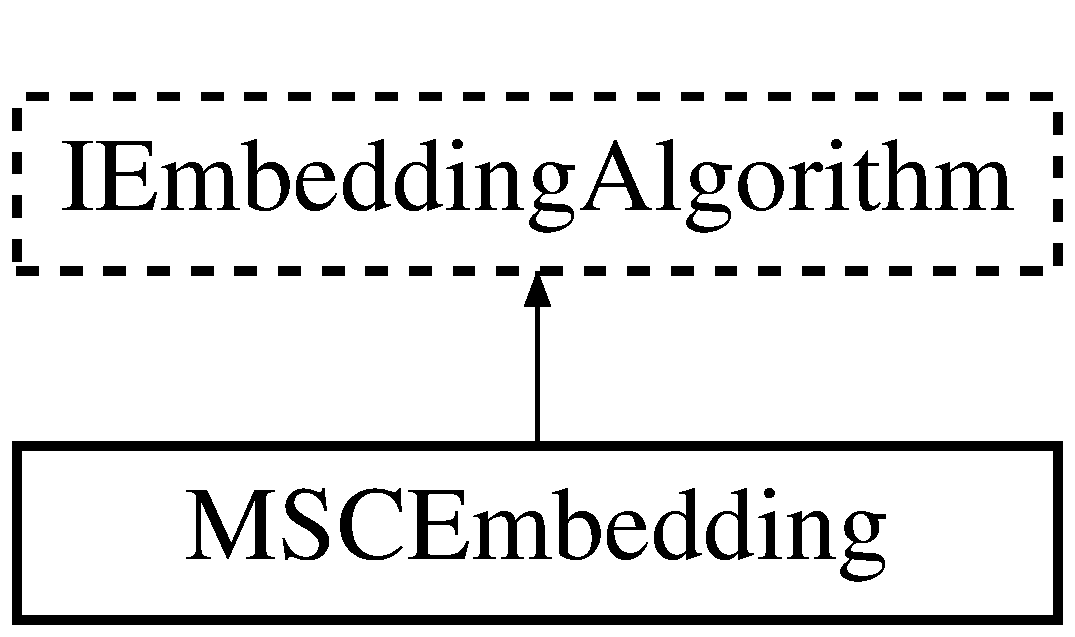
\includegraphics[height=2.000000cm]{a00088}
\end{center}
\end{figure}
\subsection*{Public Member Functions}
\begin{DoxyCompactItemize}
\item 
\hyperlink{a00088_a121cd4bb6ed8a7f520070482a2954c46}{M\+S\+C\+Embedding} (\hyperlink{a00076}{I\+Quell\+E\+Graph} \&prob, \hyperlink{a00076}{I\+Quell\+E\+Graph} \&\hyperlink{a00071_aacf081e6ad5824b339b212844eb61b63}{hardware})
\item 
virtual std\+::shared\+\_\+ptr$<$ \hyperlink{a00050}{Embedding} $>$ \hyperlink{a00088_ad1d4dd78521d916ce370ab4b109c5222}{compute\+Embedding} (std\+::map$<$ std\+::string, std\+::string $>$ parameters=std\+::map$<$ std\+::string, std\+::string $>$())
\item 
virtual std\+::string \hyperlink{a00088_a584852f9b912480086b27c1f1f14274e}{get\+Algorithm\+Name} ()
\end{DoxyCompactItemize}
\subsection*{Additional Inherited Members}


\subsection{Constructor \& Destructor Documentation}
\index{M\+S\+C\+Embedding@{M\+S\+C\+Embedding}!M\+S\+C\+Embedding@{M\+S\+C\+Embedding}}
\index{M\+S\+C\+Embedding@{M\+S\+C\+Embedding}!M\+S\+C\+Embedding@{M\+S\+C\+Embedding}}
\subsubsection[{\texorpdfstring{M\+S\+C\+Embedding(\+I\+Quell\+E\+Graph \&prob, I\+Quell\+E\+Graph \&hardware)}{MSCEmbedding(IQuellEGraph \&prob, IQuellEGraph \&hardware)}}]{\setlength{\rightskip}{0pt plus 5cm}M\+S\+C\+Embedding\+::\+M\+S\+C\+Embedding (
\begin{DoxyParamCaption}
\item[{{\bf I\+Quell\+E\+Graph} \&}]{prob, }
\item[{{\bf I\+Quell\+E\+Graph} \&}]{hardware}
\end{DoxyParamCaption}
)}\hypertarget{a00088_a121cd4bb6ed8a7f520070482a2954c46}{}\label{a00088_a121cd4bb6ed8a7f520070482a2954c46}
The Constructor, takes the problem and hardware used in this minor graph embedding.


\begin{DoxyParams}{Parameters}
{\em prob} & \\
\hline
{\em hardware} & \\
\hline
\end{DoxyParams}


\subsection{Member Function Documentation}
\index{M\+S\+C\+Embedding@{M\+S\+C\+Embedding}!compute\+Embedding@{compute\+Embedding}}
\index{compute\+Embedding@{compute\+Embedding}!M\+S\+C\+Embedding@{M\+S\+C\+Embedding}}
\subsubsection[{\texorpdfstring{compute\+Embedding(std\+::map$<$ std\+::string, std\+::string $>$ parameters=std\+::map$<$ std\+::string, std\+::string $>$())}{computeEmbedding(std::map< std::string, std::string > parameters=std::map< std::string, std::string >())}}]{\setlength{\rightskip}{0pt plus 5cm}std\+::shared\+\_\+ptr$<$ {\bf Embedding} $>$ M\+S\+C\+Embedding\+::compute\+Embedding (
\begin{DoxyParamCaption}
\item[{std\+::map$<$ std\+::string, std\+::string $>$}]{parameters = {\ttfamily std\+:\+:map$<$~std\+:\+:string,~std\+:\+:string$>$()}}
\end{DoxyParamCaption}
)\hspace{0.3cm}{\ttfamily [virtual]}}\hypertarget{a00088_ad1d4dd78521d916ce370ab4b109c5222}{}\label{a00088_ad1d4dd78521d916ce370ab4b109c5222}
Compute this embedding.


\begin{DoxyParams}{Parameters}
{\em parameters} & \\
\hline
\end{DoxyParams}


Implements \hyperlink{a00071_a0a56d5731381551efcb4c088bca6c817}{I\+Embedding\+Algorithm}.

\index{M\+S\+C\+Embedding@{M\+S\+C\+Embedding}!get\+Algorithm\+Name@{get\+Algorithm\+Name}}
\index{get\+Algorithm\+Name@{get\+Algorithm\+Name}!M\+S\+C\+Embedding@{M\+S\+C\+Embedding}}
\subsubsection[{\texorpdfstring{get\+Algorithm\+Name()}{getAlgorithmName()}}]{\setlength{\rightskip}{0pt plus 5cm}virtual std\+::string M\+S\+C\+Embedding\+::get\+Algorithm\+Name (
\begin{DoxyParamCaption}
{}
\end{DoxyParamCaption}
)\hspace{0.3cm}{\ttfamily [inline]}, {\ttfamily [virtual]}}\hypertarget{a00088_a584852f9b912480086b27c1f1f14274e}{}\label{a00088_a584852f9b912480086b27c1f1f14274e}
Return the name of this \hyperlink{a00050}{Embedding} Algorithm.

\begin{DoxyReturn}{Returns}

\end{DoxyReturn}


Implements \hyperlink{a00071_aac9fc812fb7e84b8a379ab5f60167f2c}{I\+Embedding\+Algorithm}.



The documentation for this class was generated from the following files\+:\begin{DoxyCompactItemize}
\item 
M\+S\+C\+Embedding.\+hpp\item 
M\+S\+C\+Embedding.\+cpp\end{DoxyCompactItemize}

\hypertarget{a00089}{}\section{xacc\+:\+:quantum\+:\+:Z Class Reference}
\label{a00089}\index{xacc\+::quantum\+::Z@{xacc\+::quantum\+::Z}}
Inheritance diagram for xacc\+:\+:quantum\+:\+:Z\+:\begin{figure}[H]
\begin{center}
\leavevmode
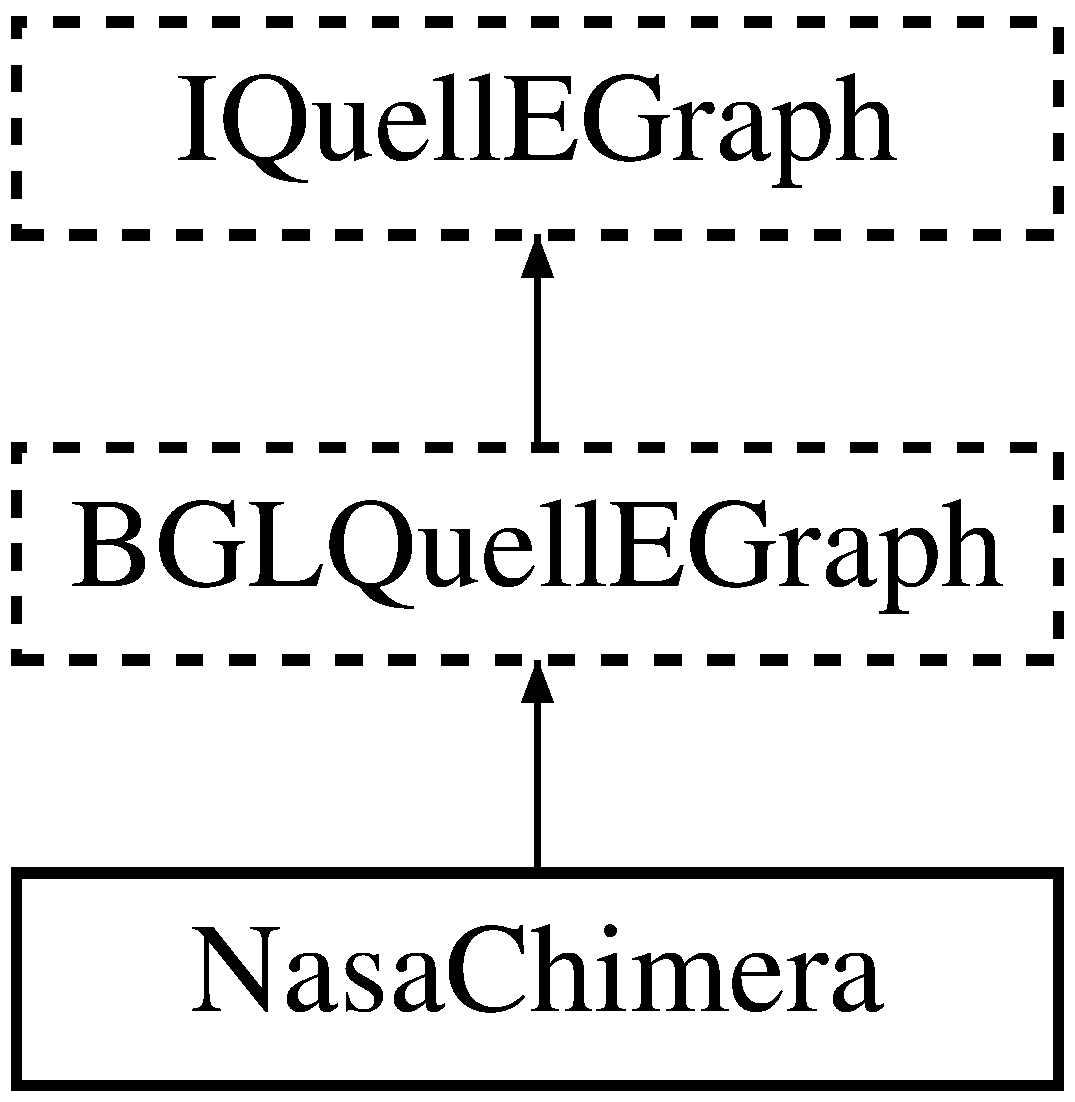
\includegraphics[height=4.000000cm]{a00089}
\end{center}
\end{figure}
\subsection*{Public Member Functions}
\begin{DoxyCompactItemize}
\item 
{\bfseries Z} (std\+::vector$<$ int $>$ qbit)\hypertarget{a00089_a5f1d311b357faed8c2665fe20cf24aeb}{}\label{a00089_a5f1d311b357faed8c2665fe20cf24aeb}

\item 
{\bfseries Z} (int qbit)\hypertarget{a00089_aa1bb7e533e7595e9ecd06879a2f8d2de}{}\label{a00089_aa1bb7e533e7595e9ecd06879a2f8d2de}

\end{DoxyCompactItemize}
\subsection*{Additional Inherited Members}


The documentation for this class was generated from the following files\+:\begin{DoxyCompactItemize}
\item 
Z.\+hpp\item 
Z.\+cpp\end{DoxyCompactItemize}

\hypertarget{a00090}{}\section{Open\+M\+P\+\_\+\+M\+P\+I\+Execution\+Model Class Reference}
\label{a00090}\index{Open\+M\+P\+\_\+\+M\+P\+I\+Execution\+Model@{Open\+M\+P\+\_\+\+M\+P\+I\+Execution\+Model}}
Inheritance diagram for Open\+M\+P\+\_\+\+M\+P\+I\+Execution\+Model\+:\begin{figure}[H]
\begin{center}
\leavevmode
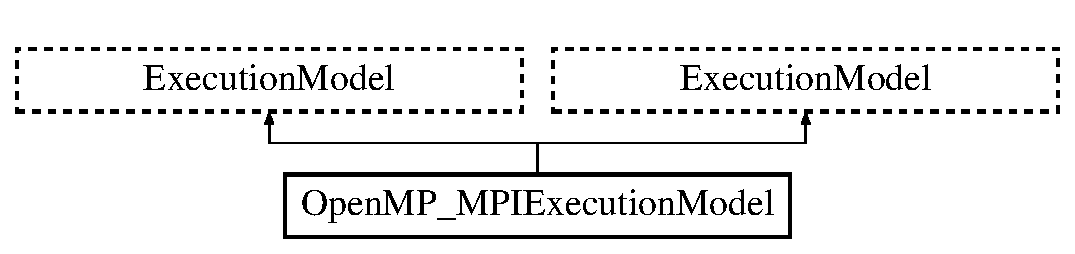
\includegraphics[height=2.000000cm]{a00090}
\end{center}
\end{figure}
\subsection*{Public Member Functions}
\begin{DoxyCompactItemize}
\item 
{\bfseries Open\+M\+P\+\_\+\+M\+P\+I\+Execution\+Model} (\hyperlink{a00092}{Parallel\+C\+M\+R\+Embedding} \&embedding)\hypertarget{a00090_a6026a68ba49eb929784ac116c6581c34}{}\label{a00090_a6026a68ba49eb929784ac116c6581c34}

\item 
virtual int {\bfseries compute\+Root\+Node} (int problem\+Vertex)\hypertarget{a00090_a5ab98063e4c317de38062314b9927492}{}\label{a00090_a5ab98063e4c317de38062314b9927492}

\item 
virtual std\+::vector$<$ Path $>$ {\bfseries compute\+Paths} (int g\+Star)\hypertarget{a00090_aa673c61e71fa3246a79ee5ce41be01b8}{}\label{a00090_aa673c61e71fa3246a79ee5ce41be01b8}

\item 
{\bfseries Open\+M\+P\+\_\+\+M\+P\+I\+Execution\+Model} (\hyperlink{a00092}{Parallel\+C\+M\+R\+Embedding} \&embedding)\hypertarget{a00090_a6026a68ba49eb929784ac116c6581c34}{}\label{a00090_a6026a68ba49eb929784ac116c6581c34}

\item 
virtual int {\bfseries compute\+Root\+Node} (int problem\+Vertex)\hypertarget{a00090_a552757725618db3523e5c7d583eafcba}{}\label{a00090_a552757725618db3523e5c7d583eafcba}

\item 
virtual std\+::vector$<$ Path $>$ {\bfseries compute\+Paths} (int g\+Star)\hypertarget{a00090_a7febfa9f71cbabbb18e76489a051e54a}{}\label{a00090_a7febfa9f71cbabbb18e76489a051e54a}

\end{DoxyCompactItemize}
\subsection*{Additional Inherited Members}


The documentation for this class was generated from the following files\+:\begin{DoxyCompactItemize}
\item 
build/quelle/aqc/embedding/impl/cmr/\+Open\+M\+P\+\_\+\+M\+P\+I\+Execution\+Model.\+hpp\item 
build/quelle/aqc/embedding/impl/cmr/\+Open\+M\+P\+\_\+\+M\+P\+I\+Execution\+Model.\+cpp\end{DoxyCompactItemize}

\hypertarget{a00091}{}\section{xacc\+:\+:Options\+Provider Class Reference}
\label{a00091}\index{xacc\+::\+Options\+Provider@{xacc\+::\+Options\+Provider}}


{\ttfamily \#include $<$Options\+Provider.\+hpp$>$}

Inheritance diagram for xacc\+:\+:Options\+Provider\+:\begin{figure}[H]
\begin{center}
\leavevmode
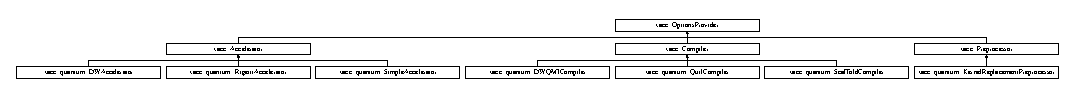
\includegraphics[height=0.824742cm]{a00091}
\end{center}
\end{figure}
\subsection*{Public Member Functions}
\begin{DoxyCompactItemize}
\item 
virtual std\+::shared\+\_\+ptr$<$ options\+\_\+description $>$ \hyperlink{a00091_a6d150954f852109bfe2c1ae90222926f}{get\+Options} ()=0
\item 
virtual \hyperlink{a00091_a7782757b419792ff346f563517eed8b8}{$\sim$\+Options\+Provider} ()
\end{DoxyCompactItemize}


\subsection{Detailed Description}
The \hyperlink{a00091}{Options\+Provider} interface enables derived subclasses to provide a description of any and all command line options that they can take to drive and control their execution and behavior. 

\subsection{Constructor \& Destructor Documentation}
\index{xacc\+::\+Options\+Provider@{xacc\+::\+Options\+Provider}!````~Options\+Provider@{$\sim$\+Options\+Provider}}
\index{````~Options\+Provider@{$\sim$\+Options\+Provider}!xacc\+::\+Options\+Provider@{xacc\+::\+Options\+Provider}}
\subsubsection[{\texorpdfstring{$\sim$\+Options\+Provider()}{~OptionsProvider()}}]{\setlength{\rightskip}{0pt plus 5cm}virtual xacc\+::\+Options\+Provider\+::$\sim$\+Options\+Provider (
\begin{DoxyParamCaption}
{}
\end{DoxyParamCaption}
)\hspace{0.3cm}{\ttfamily [inline]}, {\ttfamily [virtual]}}\hypertarget{a00091_a7782757b419792ff346f563517eed8b8}{}\label{a00091_a7782757b419792ff346f563517eed8b8}
The destructor 

\subsection{Member Function Documentation}
\index{xacc\+::\+Options\+Provider@{xacc\+::\+Options\+Provider}!get\+Options@{get\+Options}}
\index{get\+Options@{get\+Options}!xacc\+::\+Options\+Provider@{xacc\+::\+Options\+Provider}}
\subsubsection[{\texorpdfstring{get\+Options()=0}{getOptions()=0}}]{\setlength{\rightskip}{0pt plus 5cm}virtual std\+::shared\+\_\+ptr$<$options\+\_\+description$>$ xacc\+::\+Options\+Provider\+::get\+Options (
\begin{DoxyParamCaption}
{}
\end{DoxyParamCaption}
)\hspace{0.3cm}{\ttfamily [pure virtual]}}\hypertarget{a00091_a6d150954f852109bfe2c1ae90222926f}{}\label{a00091_a6d150954f852109bfe2c1ae90222926f}
Return a Boost options\+\_\+description instance that describes the options available for this derived subclass. 

Implemented in \hyperlink{a00017_a98c9eda6b54367c75667ecfbbf167979}{xacc\+::\+Accelerator}, \hyperlink{a00042_a09926db9f99706307ae6ce5b56845bca}{xacc\+::quantum\+::\+D\+W\+Accelerator}, \hyperlink{a00112_a9ee9e62aecbccf193894ca3388676f9f}{xacc\+::quantum\+::\+Rigetti\+Accelerator}, \hyperlink{a00034_a9f5a8965c9c2dd895016d18264ebbe92}{xacc\+::\+Compiler}, \hyperlink{a00047_a0851334cc33b5b1da2694150a0a1a43c}{xacc\+::quantum\+::\+D\+W\+Q\+M\+I\+Compiler}, and \hyperlink{a00094_a96f5600ea47628b66917c7b90250e7f1}{xacc\+::\+Preprocessor}.



The documentation for this class was generated from the following file\+:\begin{DoxyCompactItemize}
\item 
Options\+Provider.\+hpp\end{DoxyCompactItemize}

\hypertarget{a00092}{}\section{Encoded\+Input\+Stream$<$ Encoding, Input\+Byte\+Stream $>$ Class Template Reference}
\label{a00092}\index{Encoded\+Input\+Stream$<$ Encoding, Input\+Byte\+Stream $>$@{Encoded\+Input\+Stream$<$ Encoding, Input\+Byte\+Stream $>$}}


Input byte stream wrapper with a statically bound encoding.  




{\ttfamily \#include $<$encodedstream.\+h$>$}

\subsection*{Public Types}
\begin{DoxyCompactItemize}
\item 
typedef Encoding\+::\+Ch {\bfseries Ch}\hypertarget{a00092_acc387a1364390da244bbb1ab07bdceca}{}\label{a00092_acc387a1364390da244bbb1ab07bdceca}

\end{DoxyCompactItemize}
\subsection*{Public Member Functions}
\begin{DoxyCompactItemize}
\item 
{\bfseries Encoded\+Input\+Stream} (Input\+Byte\+Stream \&is)\hypertarget{a00092_a17f8e629500f6ae71cb72d1d63bf41fd}{}\label{a00092_a17f8e629500f6ae71cb72d1d63bf41fd}

\item 
Ch {\bfseries Peek} () const \hypertarget{a00092_abda3b0c141254343f4c481f67d52b423}{}\label{a00092_abda3b0c141254343f4c481f67d52b423}

\item 
Ch {\bfseries Take} ()\hypertarget{a00092_ab42cd57581bf62e42af471583e5b8377}{}\label{a00092_ab42cd57581bf62e42af471583e5b8377}

\item 
size\+\_\+t {\bfseries Tell} () const \hypertarget{a00092_a34cdb99fd81cd211f71903348e9c986f}{}\label{a00092_a34cdb99fd81cd211f71903348e9c986f}

\item 
void {\bfseries Put} (Ch)\hypertarget{a00092_afea36b666a44bd4adeabfcab7b68a322}{}\label{a00092_afea36b666a44bd4adeabfcab7b68a322}

\item 
void {\bfseries Flush} ()\hypertarget{a00092_aa4415bf4b97dd01e8c3de0ad7a161724}{}\label{a00092_aa4415bf4b97dd01e8c3de0ad7a161724}

\item 
Ch $\ast$ {\bfseries Put\+Begin} ()\hypertarget{a00092_ad97f7a549a8622c61b7fb2c63fedd69b}{}\label{a00092_ad97f7a549a8622c61b7fb2c63fedd69b}

\item 
size\+\_\+t {\bfseries Put\+End} (Ch $\ast$)\hypertarget{a00092_a83fe5ed281413d6005d1b324730e8bed}{}\label{a00092_a83fe5ed281413d6005d1b324730e8bed}

\end{DoxyCompactItemize}


\subsection{Detailed Description}
\subsubsection*{template$<$typename Encoding, typename Input\+Byte\+Stream$>$\\*
class Encoded\+Input\+Stream$<$ Encoding, Input\+Byte\+Stream $>$}

Input byte stream wrapper with a statically bound encoding. 


\begin{DoxyTemplParams}{Template Parameters}
{\em Encoding} & The interpretation of encoding of the stream. Either \hyperlink{a00333}{U\+T\+F8}, \hyperlink{a00329}{U\+T\+F16\+LE}, \hyperlink{a00328}{U\+T\+F16\+BE}, \hyperlink{a00332}{U\+T\+F32\+LE}, \hyperlink{a00331}{U\+T\+F32\+BE}. \\
\hline
{\em Input\+Byte\+Stream} & Type of input byte stream. For example, \hyperlink{a00101}{File\+Read\+Stream}. \\
\hline
\end{DoxyTemplParams}


The documentation for this class was generated from the following file\+:\begin{DoxyCompactItemize}
\item 
encodedstream.\+h\end{DoxyCompactItemize}

\hypertarget{a00093}{}\section{xacc\+:\+:quantum\+:\+:Parallel\+C\+M\+R\+Embedding Class Reference}
\label{a00093}\index{xacc\+::quantum\+::\+Parallel\+C\+M\+R\+Embedding@{xacc\+::quantum\+::\+Parallel\+C\+M\+R\+Embedding}}
Inheritance diagram for xacc\+:\+:quantum\+:\+:Parallel\+C\+M\+R\+Embedding\+:\begin{figure}[H]
\begin{center}
\leavevmode
\includegraphics[height=3.000000cm]{a00093}
\end{center}
\end{figure}
\subsection*{Public Member Functions}
\begin{DoxyCompactItemize}
\item 
\hyperlink{a00093_a7bad0996c759a5c3a8f325b4c3eb7b90}{Parallel\+C\+M\+R\+Embedding} (std\+::shared\+\_\+ptr$<$ \hyperlink{a00043}{D\+W\+Graph} $>$ prob, std\+::shared\+\_\+ptr$<$ \hyperlink{a00064}{Accelerator\+Graph} $>$ \hyperlink{a00051_a63d22756b8ad0f1a689b46d17a0ce81e}{hardware})
\item 
virtual void \hyperlink{a00093_a2d9a99786af28f38134f0243d231bb35}{compute\+Vertex\+Model} (int prob\+Vertex)
\item 
virtual bool \hyperlink{a00093_a74606fda2c0542c2d197146787969bd4}{is\+Valid} ()
\item 
virtual void \hyperlink{a00093_a55ba8c7ae717cbfa8a57503116536344}{add\+To\+Vertex\+Model} (int prob\+Vertex, int hardware\+Vertex)
\item 
int \hyperlink{a00093_a7f18154f9ba79fb4bee03543e75cddb5}{get\+N\+Represented} (int vertex)
\item 
bool \hyperlink{a00093_a70955f1c3534bc9da12c3956b11a7820}{is\+Vertex\+Used} (int vertex)
\item 
void \hyperlink{a00093_ae5a7423f3c2655a8c2364bc5c389b796}{set\+Ghost\+Vertices} (std\+::map$<$ int, int $>$ map)
\item 
void {\bfseries set\+Execution\+Model} (std\+::string model)\hypertarget{a00093_a51a93e8c46a997c48c7514763770c079}{}\label{a00093_a51a93e8c46a997c48c7514763770c079}

\item 
bool \hyperlink{a00093_a6fbb695c060ff00be3134c874ff82a6c}{is\+Ghost\+Vertex} (int g)
\item 
std\+::shared\+\_\+ptr$<$ \hyperlink{a00064}{Accelerator\+Graph} $>$ \& {\bfseries get\+Hardware} ()\hypertarget{a00093_a385340fd3fe411251d2529fbc2f4a5a4}{}\label{a00093_a385340fd3fe411251d2529fbc2f4a5a4}

\item 
std\+::shared\+\_\+ptr$<$ \hyperlink{a00043}{D\+W\+Graph} $>$ \& {\bfseries get\+Problem} ()\hypertarget{a00093_a0b8aec8a62d1c552174bce92a080cc04}{}\label{a00093_a0b8aec8a62d1c552174bce92a080cc04}

\item 
std\+::map$<$ int, int $>$ {\bfseries get\+Prob\+To\+Ghost\+Map} ()\hypertarget{a00093_aa835ef8197250447500f2e17c618a353}{}\label{a00093_aa835ef8197250447500f2e17c618a353}

\end{DoxyCompactItemize}
\subsection*{Protected Attributes}
\begin{DoxyCompactItemize}
\item 
std\+::string {\bfseries execution\+Model}\hypertarget{a00093_a0c17fd8d18fa8d30b4e11a0521b9edfd}{}\label{a00093_a0c17fd8d18fa8d30b4e11a0521b9edfd}

\item 
int \hyperlink{a00093_aaa15f33fe4407f8508015cbf8e614782}{hardware\+Diameter}
\item 
mpi\+::communicator \& \hyperlink{a00093_a2bb97f1bc1a2791e06eb094fc631a056}{comm}
\item 
int \hyperlink{a00093_a25e19b46e2ece70638325eefecf5c5b9}{rank}
\item 
std\+::map$<$ int, int $>$ \hyperlink{a00093_ae16bfd68d24b66ac42c466bdd332d761}{prob\+Verts\+To\+Ghost\+Verts}
\item 
std\+::vector$<$ int $>$ \hyperlink{a00093_a116a73f60557e233a41da7a46d8175db}{local\+Vertices}
\item 
std\+::map$<$ int, int $>$ \hyperlink{a00093_abfa929179ced4ddb425f76c238e560f8}{vertex\+Use\+Count}
\item 
bool {\bfseries computed\+Random\+Vertex} = false\hypertarget{a00093_a7adc585f5a21989029dc395a9fd5b821}{}\label{a00093_a7adc585f5a21989029dc395a9fd5b821}

\end{DoxyCompactItemize}


\subsection{Constructor \& Destructor Documentation}
\index{xacc\+::quantum\+::\+Parallel\+C\+M\+R\+Embedding@{xacc\+::quantum\+::\+Parallel\+C\+M\+R\+Embedding}!Parallel\+C\+M\+R\+Embedding@{Parallel\+C\+M\+R\+Embedding}}
\index{Parallel\+C\+M\+R\+Embedding@{Parallel\+C\+M\+R\+Embedding}!xacc\+::quantum\+::\+Parallel\+C\+M\+R\+Embedding@{xacc\+::quantum\+::\+Parallel\+C\+M\+R\+Embedding}}
\subsubsection[{\texorpdfstring{Parallel\+C\+M\+R\+Embedding(std\+::shared\+\_\+ptr$<$ D\+W\+Graph $>$ prob, std\+::shared\+\_\+ptr$<$ Accelerator\+Graph $>$ hardware)}{ParallelCMREmbedding(std::shared\_ptr< DWGraph > prob, std::shared\_ptr< AcceleratorGraph > hardware)}}]{\setlength{\rightskip}{0pt plus 5cm}Parallel\+C\+M\+R\+Embedding\+::\+Parallel\+C\+M\+R\+Embedding (
\begin{DoxyParamCaption}
\item[{std\+::shared\+\_\+ptr$<$ {\bf D\+W\+Graph} $>$}]{prob, }
\item[{std\+::shared\+\_\+ptr$<$ {\bf Accelerator\+Graph} $>$}]{hardware}
\end{DoxyParamCaption}
)}\hypertarget{a00093_a7bad0996c759a5c3a8f325b4c3eb7b90}{}\label{a00093_a7bad0996c759a5c3a8f325b4c3eb7b90}
The constructor. Must be instantiated with references to the problem and hardware graphs for this embedding. 

\subsection{Member Function Documentation}
\index{xacc\+::quantum\+::\+Parallel\+C\+M\+R\+Embedding@{xacc\+::quantum\+::\+Parallel\+C\+M\+R\+Embedding}!add\+To\+Vertex\+Model@{add\+To\+Vertex\+Model}}
\index{add\+To\+Vertex\+Model@{add\+To\+Vertex\+Model}!xacc\+::quantum\+::\+Parallel\+C\+M\+R\+Embedding@{xacc\+::quantum\+::\+Parallel\+C\+M\+R\+Embedding}}
\subsubsection[{\texorpdfstring{add\+To\+Vertex\+Model(int prob\+Vertex, int hardware\+Vertex)}{addToVertexModel(int probVertex, int hardwareVertex)}}]{\setlength{\rightskip}{0pt plus 5cm}void Parallel\+C\+M\+R\+Embedding\+::add\+To\+Vertex\+Model (
\begin{DoxyParamCaption}
\item[{int}]{prob\+Vertex, }
\item[{int}]{hardware\+Vertex}
\end{DoxyParamCaption}
)\hspace{0.3cm}{\ttfamily [virtual]}}\hypertarget{a00093_a55ba8c7ae717cbfa8a57503116536344}{}\label{a00093_a55ba8c7ae717cbfa8a57503116536344}
Add the given hardware vertex to the problem vertex\textquotesingle{}s vertex model. This also connects the hardware vertex to the models ghost vertex.


\begin{DoxyParams}{Parameters}
{\em prob\+Vertex} & \\
\hline
{\em hardware\+Vertex} & \\
\hline
\end{DoxyParams}
\index{xacc\+::quantum\+::\+Parallel\+C\+M\+R\+Embedding@{xacc\+::quantum\+::\+Parallel\+C\+M\+R\+Embedding}!compute\+Vertex\+Model@{compute\+Vertex\+Model}}
\index{compute\+Vertex\+Model@{compute\+Vertex\+Model}!xacc\+::quantum\+::\+Parallel\+C\+M\+R\+Embedding@{xacc\+::quantum\+::\+Parallel\+C\+M\+R\+Embedding}}
\subsubsection[{\texorpdfstring{compute\+Vertex\+Model(int prob\+Vertex)}{computeVertexModel(int probVertex)}}]{\setlength{\rightskip}{0pt plus 5cm}void Parallel\+C\+M\+R\+Embedding\+::compute\+Vertex\+Model (
\begin{DoxyParamCaption}
\item[{int}]{prob\+Vertex}
\end{DoxyParamCaption}
)\hspace{0.3cm}{\ttfamily [virtual]}}\hypertarget{a00093_a2d9a99786af28f38134f0243d231bb35}{}\label{a00093_a2d9a99786af28f38134f0243d231bb35}
This method computes a minimal Vertex\+Model for the given problem vertex. \index{xacc\+::quantum\+::\+Parallel\+C\+M\+R\+Embedding@{xacc\+::quantum\+::\+Parallel\+C\+M\+R\+Embedding}!get\+N\+Represented@{get\+N\+Represented}}
\index{get\+N\+Represented@{get\+N\+Represented}!xacc\+::quantum\+::\+Parallel\+C\+M\+R\+Embedding@{xacc\+::quantum\+::\+Parallel\+C\+M\+R\+Embedding}}
\subsubsection[{\texorpdfstring{get\+N\+Represented(int vertex)}{getNRepresented(int vertex)}}]{\setlength{\rightskip}{0pt plus 5cm}int Parallel\+C\+M\+R\+Embedding\+::get\+N\+Represented (
\begin{DoxyParamCaption}
\item[{int}]{vertex}
\end{DoxyParamCaption}
)}\hypertarget{a00093_a7f18154f9ba79fb4bee03543e75cddb5}{}\label{a00093_a7f18154f9ba79fb4bee03543e75cddb5}
This operation returns the number of vertex models already using the provided vertex. \index{xacc\+::quantum\+::\+Parallel\+C\+M\+R\+Embedding@{xacc\+::quantum\+::\+Parallel\+C\+M\+R\+Embedding}!is\+Ghost\+Vertex@{is\+Ghost\+Vertex}}
\index{is\+Ghost\+Vertex@{is\+Ghost\+Vertex}!xacc\+::quantum\+::\+Parallel\+C\+M\+R\+Embedding@{xacc\+::quantum\+::\+Parallel\+C\+M\+R\+Embedding}}
\subsubsection[{\texorpdfstring{is\+Ghost\+Vertex(int g)}{isGhostVertex(int g)}}]{\setlength{\rightskip}{0pt plus 5cm}bool Parallel\+C\+M\+R\+Embedding\+::is\+Ghost\+Vertex (
\begin{DoxyParamCaption}
\item[{int}]{g}
\end{DoxyParamCaption}
)}\hypertarget{a00093_a6fbb695c060ff00be3134c874ff82a6c}{}\label{a00093_a6fbb695c060ff00be3134c874ff82a6c}
Return true if the given vertex is a ghost vertex.


\begin{DoxyParams}{Parameters}
{\em g} & \\
\hline
\end{DoxyParams}
\begin{DoxyReturn}{Returns}

\end{DoxyReturn}
\index{xacc\+::quantum\+::\+Parallel\+C\+M\+R\+Embedding@{xacc\+::quantum\+::\+Parallel\+C\+M\+R\+Embedding}!is\+Valid@{is\+Valid}}
\index{is\+Valid@{is\+Valid}!xacc\+::quantum\+::\+Parallel\+C\+M\+R\+Embedding@{xacc\+::quantum\+::\+Parallel\+C\+M\+R\+Embedding}}
\subsubsection[{\texorpdfstring{is\+Valid()}{isValid()}}]{\setlength{\rightskip}{0pt plus 5cm}bool Parallel\+C\+M\+R\+Embedding\+::is\+Valid (
\begin{DoxyParamCaption}
{}
\end{DoxyParamCaption}
)\hspace{0.3cm}{\ttfamily [virtual]}}\hypertarget{a00093_a74606fda2c0542c2d197146787969bd4}{}\label{a00093_a74606fda2c0542c2d197146787969bd4}
Return true if the embedding is a valid one. \begin{DoxyReturn}{Returns}

\end{DoxyReturn}


Implements \hyperlink{a00051}{xacc\+::quantum\+::\+Embedding}.

\index{xacc\+::quantum\+::\+Parallel\+C\+M\+R\+Embedding@{xacc\+::quantum\+::\+Parallel\+C\+M\+R\+Embedding}!is\+Vertex\+Used@{is\+Vertex\+Used}}
\index{is\+Vertex\+Used@{is\+Vertex\+Used}!xacc\+::quantum\+::\+Parallel\+C\+M\+R\+Embedding@{xacc\+::quantum\+::\+Parallel\+C\+M\+R\+Embedding}}
\subsubsection[{\texorpdfstring{is\+Vertex\+Used(int vertex)}{isVertexUsed(int vertex)}}]{\setlength{\rightskip}{0pt plus 5cm}bool Parallel\+C\+M\+R\+Embedding\+::is\+Vertex\+Used (
\begin{DoxyParamCaption}
\item[{int}]{vertex}
\end{DoxyParamCaption}
)}\hypertarget{a00093_a70955f1c3534bc9da12c3956b11a7820}{}\label{a00093_a70955f1c3534bc9da12c3956b11a7820}
This operation returns true if the provided vertex has been used by another vertex model. \index{xacc\+::quantum\+::\+Parallel\+C\+M\+R\+Embedding@{xacc\+::quantum\+::\+Parallel\+C\+M\+R\+Embedding}!set\+Ghost\+Vertices@{set\+Ghost\+Vertices}}
\index{set\+Ghost\+Vertices@{set\+Ghost\+Vertices}!xacc\+::quantum\+::\+Parallel\+C\+M\+R\+Embedding@{xacc\+::quantum\+::\+Parallel\+C\+M\+R\+Embedding}}
\subsubsection[{\texorpdfstring{set\+Ghost\+Vertices(std\+::map$<$ int, int $>$ map)}{setGhostVertices(std::map< int, int > map)}}]{\setlength{\rightskip}{0pt plus 5cm}void xacc\+::quantum\+::\+Parallel\+C\+M\+R\+Embedding\+::set\+Ghost\+Vertices (
\begin{DoxyParamCaption}
\item[{std\+::map$<$ int, int $>$}]{map}
\end{DoxyParamCaption}
)\hspace{0.3cm}{\ttfamily [inline]}}\hypertarget{a00093_ae5a7423f3c2655a8c2364bc5c389b796}{}\label{a00093_ae5a7423f3c2655a8c2364bc5c389b796}
Set the map of problem vertices to their ghost vertex representation in the hardware.


\begin{DoxyParams}{Parameters}
{\em map} & \\
\hline
\end{DoxyParams}


\subsection{Member Data Documentation}
\index{xacc\+::quantum\+::\+Parallel\+C\+M\+R\+Embedding@{xacc\+::quantum\+::\+Parallel\+C\+M\+R\+Embedding}!comm@{comm}}
\index{comm@{comm}!xacc\+::quantum\+::\+Parallel\+C\+M\+R\+Embedding@{xacc\+::quantum\+::\+Parallel\+C\+M\+R\+Embedding}}
\subsubsection[{\texorpdfstring{comm}{comm}}]{\setlength{\rightskip}{0pt plus 5cm}mpi\+::communicator\& xacc\+::quantum\+::\+Parallel\+C\+M\+R\+Embedding\+::comm\hspace{0.3cm}{\ttfamily [protected]}}\hypertarget{a00093_a2bb97f1bc1a2791e06eb094fc631a056}{}\label{a00093_a2bb97f1bc1a2791e06eb094fc631a056}
Reference to the M\+PI communicator object. \index{xacc\+::quantum\+::\+Parallel\+C\+M\+R\+Embedding@{xacc\+::quantum\+::\+Parallel\+C\+M\+R\+Embedding}!hardware\+Diameter@{hardware\+Diameter}}
\index{hardware\+Diameter@{hardware\+Diameter}!xacc\+::quantum\+::\+Parallel\+C\+M\+R\+Embedding@{xacc\+::quantum\+::\+Parallel\+C\+M\+R\+Embedding}}
\subsubsection[{\texorpdfstring{hardware\+Diameter}{hardwareDiameter}}]{\setlength{\rightskip}{0pt plus 5cm}int xacc\+::quantum\+::\+Parallel\+C\+M\+R\+Embedding\+::hardware\+Diameter\hspace{0.3cm}{\ttfamily [protected]}}\hypertarget{a00093_aaa15f33fe4407f8508015cbf8e614782}{}\label{a00093_aaa15f33fe4407f8508015cbf8e614782}
Reference to the hardware diameter, we store this to be used in the bias calculation \index{xacc\+::quantum\+::\+Parallel\+C\+M\+R\+Embedding@{xacc\+::quantum\+::\+Parallel\+C\+M\+R\+Embedding}!local\+Vertices@{local\+Vertices}}
\index{local\+Vertices@{local\+Vertices}!xacc\+::quantum\+::\+Parallel\+C\+M\+R\+Embedding@{xacc\+::quantum\+::\+Parallel\+C\+M\+R\+Embedding}}
\subsubsection[{\texorpdfstring{local\+Vertices}{localVertices}}]{\setlength{\rightskip}{0pt plus 5cm}std\+::vector$<$int$>$ xacc\+::quantum\+::\+Parallel\+C\+M\+R\+Embedding\+::local\+Vertices\hspace{0.3cm}{\ttfamily [protected]}}\hypertarget{a00093_a116a73f60557e233a41da7a46d8175db}{}\label{a00093_a116a73f60557e233a41da7a46d8175db}
The total list of vertices that are local to this processor \index{xacc\+::quantum\+::\+Parallel\+C\+M\+R\+Embedding@{xacc\+::quantum\+::\+Parallel\+C\+M\+R\+Embedding}!prob\+Verts\+To\+Ghost\+Verts@{prob\+Verts\+To\+Ghost\+Verts}}
\index{prob\+Verts\+To\+Ghost\+Verts@{prob\+Verts\+To\+Ghost\+Verts}!xacc\+::quantum\+::\+Parallel\+C\+M\+R\+Embedding@{xacc\+::quantum\+::\+Parallel\+C\+M\+R\+Embedding}}
\subsubsection[{\texorpdfstring{prob\+Verts\+To\+Ghost\+Verts}{probVertsToGhostVerts}}]{\setlength{\rightskip}{0pt plus 5cm}std\+::map$<$int, int$>$ xacc\+::quantum\+::\+Parallel\+C\+M\+R\+Embedding\+::prob\+Verts\+To\+Ghost\+Verts\hspace{0.3cm}{\ttfamily [protected]}}\hypertarget{a00093_ae16bfd68d24b66ac42c466bdd332d761}{}\label{a00093_ae16bfd68d24b66ac42c466bdd332d761}
A map from problem vertices to their ghost vertex representation in the hardware \index{xacc\+::quantum\+::\+Parallel\+C\+M\+R\+Embedding@{xacc\+::quantum\+::\+Parallel\+C\+M\+R\+Embedding}!rank@{rank}}
\index{rank@{rank}!xacc\+::quantum\+::\+Parallel\+C\+M\+R\+Embedding@{xacc\+::quantum\+::\+Parallel\+C\+M\+R\+Embedding}}
\subsubsection[{\texorpdfstring{rank}{rank}}]{\setlength{\rightskip}{0pt plus 5cm}int xacc\+::quantum\+::\+Parallel\+C\+M\+R\+Embedding\+::rank\hspace{0.3cm}{\ttfamily [protected]}}\hypertarget{a00093_a25e19b46e2ece70638325eefecf5c5b9}{}\label{a00093_a25e19b46e2ece70638325eefecf5c5b9}
Reference to the local process rank \index{xacc\+::quantum\+::\+Parallel\+C\+M\+R\+Embedding@{xacc\+::quantum\+::\+Parallel\+C\+M\+R\+Embedding}!vertex\+Use\+Count@{vertex\+Use\+Count}}
\index{vertex\+Use\+Count@{vertex\+Use\+Count}!xacc\+::quantum\+::\+Parallel\+C\+M\+R\+Embedding@{xacc\+::quantum\+::\+Parallel\+C\+M\+R\+Embedding}}
\subsubsection[{\texorpdfstring{vertex\+Use\+Count}{vertexUseCount}}]{\setlength{\rightskip}{0pt plus 5cm}std\+::map$<$int, int$>$ xacc\+::quantum\+::\+Parallel\+C\+M\+R\+Embedding\+::vertex\+Use\+Count\hspace{0.3cm}{\ttfamily [protected]}}\hypertarget{a00093_abfa929179ced4ddb425f76c238e560f8}{}\label{a00093_abfa929179ced4ddb425f76c238e560f8}
The map of hardware vertices to their embedding use count. 

The documentation for this class was generated from the following files\+:\begin{DoxyCompactItemize}
\item 
quantum/aqc/compiler/cmr/\+Parallel\+C\+M\+R\+Embedding.\+hpp\item 
quantum/aqc/compiler/cmr/\+Parallel\+C\+M\+R\+Embedding.\+cpp\end{DoxyCompactItemize}

\hypertarget{a00094}{}\section{xacc\+:\+:Preprocessor Class Reference}
\label{a00094}\index{xacc\+::\+Preprocessor@{xacc\+::\+Preprocessor}}


{\ttfamily \#include $<$Preprocessor.\+hpp$>$}

Inheritance diagram for xacc\+:\+:Preprocessor\+:\begin{figure}[H]
\begin{center}
\leavevmode
\includegraphics[height=3.000000cm]{a00094}
\end{center}
\end{figure}
\subsection*{Public Member Functions}
\begin{DoxyCompactItemize}
\item 
virtual const std\+::string \hyperlink{a00094_ae59b5a2963f8bcc84b590a83f4749e19}{process} (const std\+::string \&source, std\+::shared\+\_\+ptr$<$ \hyperlink{a00034}{Compiler} $>$ compiler, std\+::shared\+\_\+ptr$<$ \hyperlink{a00017}{Accelerator} $>$ accelerator)=0
\item 
virtual const std\+::string \hyperlink{a00094_a36671f4c062d61e230306edc404774cd}{get\+Name} ()=0
\item 
virtual std\+::shared\+\_\+ptr$<$ options\+\_\+description $>$ \hyperlink{a00094_a96f5600ea47628b66917c7b90250e7f1}{get\+Options} ()
\end{DoxyCompactItemize}


\subsection{Detailed Description}
The \hyperlink{a00094}{Preprocessor} interface provides a mechanism for processing quantum kernel source code before compilation takes place. Realizations of this interface implement the process method which takes as input the source code to process, and the compiler and accelerator this code is targeted at. 

\subsection{Member Function Documentation}
\index{xacc\+::\+Preprocessor@{xacc\+::\+Preprocessor}!get\+Name@{get\+Name}}
\index{get\+Name@{get\+Name}!xacc\+::\+Preprocessor@{xacc\+::\+Preprocessor}}
\subsubsection[{\texorpdfstring{get\+Name()=0}{getName()=0}}]{\setlength{\rightskip}{0pt plus 5cm}virtual const std\+::string xacc\+::\+Preprocessor\+::get\+Name (
\begin{DoxyParamCaption}
{}
\end{DoxyParamCaption}
)\hspace{0.3cm}{\ttfamily [pure virtual]}}\hypertarget{a00094_a36671f4c062d61e230306edc404774cd}{}\label{a00094_a36671f4c062d61e230306edc404774cd}
Return the name of this \hyperlink{a00094}{Preprocessor}

\begin{DoxyReturn}{Returns}
name The name of this preprocessor 
\end{DoxyReturn}


Implemented in \hyperlink{a00084_af74db6b7f3adeb7d203777f5ce450491}{xacc\+::quantum\+::\+Kernel\+Replacement\+Preprocessor}.

\index{xacc\+::\+Preprocessor@{xacc\+::\+Preprocessor}!get\+Options@{get\+Options}}
\index{get\+Options@{get\+Options}!xacc\+::\+Preprocessor@{xacc\+::\+Preprocessor}}
\subsubsection[{\texorpdfstring{get\+Options()}{getOptions()}}]{\setlength{\rightskip}{0pt plus 5cm}virtual std\+::shared\+\_\+ptr$<$options\+\_\+description$>$ xacc\+::\+Preprocessor\+::get\+Options (
\begin{DoxyParamCaption}
{}
\end{DoxyParamCaption}
)\hspace{0.3cm}{\ttfamily [inline]}, {\ttfamily [virtual]}}\hypertarget{a00094_a96f5600ea47628b66917c7b90250e7f1}{}\label{a00094_a96f5600ea47628b66917c7b90250e7f1}
Return an empty options\+\_\+description, this is for subclasses to implement. 

Implements \hyperlink{a00091_a6d150954f852109bfe2c1ae90222926f}{xacc\+::\+Options\+Provider}.

\index{xacc\+::\+Preprocessor@{xacc\+::\+Preprocessor}!process@{process}}
\index{process@{process}!xacc\+::\+Preprocessor@{xacc\+::\+Preprocessor}}
\subsubsection[{\texorpdfstring{process(const std\+::string \&source, std\+::shared\+\_\+ptr$<$ Compiler $>$ compiler, std\+::shared\+\_\+ptr$<$ Accelerator $>$ accelerator)=0}{process(const std::string \&source, std::shared\_ptr< Compiler > compiler, std::shared\_ptr< Accelerator > accelerator)=0}}]{\setlength{\rightskip}{0pt plus 5cm}virtual const std\+::string xacc\+::\+Preprocessor\+::process (
\begin{DoxyParamCaption}
\item[{const std\+::string \&}]{source, }
\item[{std\+::shared\+\_\+ptr$<$ {\bf Compiler} $>$}]{compiler, }
\item[{std\+::shared\+\_\+ptr$<$ {\bf Accelerator} $>$}]{accelerator}
\end{DoxyParamCaption}
)\hspace{0.3cm}{\ttfamily [pure virtual]}}\hypertarget{a00094_ae59b5a2963f8bcc84b590a83f4749e19}{}\label{a00094_ae59b5a2963f8bcc84b590a83f4749e19}
This method is to be implemented by subclasses to take in a kernel source string and process it in an isomorphic manner, and returns the processed source code.


\begin{DoxyParams}{Parameters}
{\em src} & The unprocessed kernel source code \\
\hline
{\em compiler} & The compiler being used to compile the code \\
\hline
{\em accelerator} & The \hyperlink{a00017}{Accelerator} this code will be run on\\
\hline
\end{DoxyParams}
\begin{DoxyReturn}{Returns}
processed\+Src The processed kernel source code 
\end{DoxyReturn}


Implemented in \hyperlink{a00084_ad4f9ba1f83ea45ed376f36e3853c668d}{xacc\+::quantum\+::\+Kernel\+Replacement\+Preprocessor}.



The documentation for this class was generated from the following file\+:\begin{DoxyCompactItemize}
\item 
Preprocessor.\+hpp\end{DoxyCompactItemize}

\hypertarget{a00095}{}\section{rapidjson\+:\+:Encoding Class Reference}
\label{a00095}\index{rapidjson\+::\+Encoding@{rapidjson\+::\+Encoding}}


Concept for encoding of Unicode characters.  




{\ttfamily \#include $<$encodings.\+h$>$}



\subsection{Detailed Description}
Concept for encoding of Unicode characters. 


\begin{DoxyCode}
concept Encoding \{
    \textcolor{keyword}{typename} Ch;    

    \textcolor{keyword}{enum} \{ supportUnicode = 1 \}; \textcolor{comment}{// or 0 if not supporting unicode}

    \textcolor{keyword}{template}<\textcolor{keyword}{typename} OutputStream>
    \textcolor{keyword}{static} \textcolor{keywordtype}{void} Encode(OutputStream& os, \textcolor{keywordtype}{unsigned} codepoint);

    \textcolor{keyword}{template} <\textcolor{keyword}{typename} InputStream>
    \textcolor{keyword}{static} \textcolor{keywordtype}{bool} Decode(InputStream& is, \textcolor{keywordtype}{unsigned}* codepoint);

    \textcolor{keyword}{template} <\textcolor{keyword}{typename} InputStream, \textcolor{keyword}{typename} OutputStream>
    \textcolor{keyword}{static} \textcolor{keywordtype}{bool} Validate(InputStream& is, OutputStream& os);

    \textcolor{comment}{// The following functions are deal with byte streams.}

    \textcolor{keyword}{template} <\textcolor{keyword}{typename} InputByteStream>
    \textcolor{keyword}{static} CharType TakeBOM(InputByteStream& is);

    \textcolor{keyword}{template} <\textcolor{keyword}{typename} InputByteStream>
    \textcolor{keyword}{static} Ch Take(InputByteStream& is);

    \textcolor{keyword}{template} <\textcolor{keyword}{typename} OutputByteStream>
    \textcolor{keyword}{static} \textcolor{keywordtype}{void} PutBOM(OutputByteStream& os);

    \textcolor{keyword}{template} <\textcolor{keyword}{typename} OutputByteStream>
    \textcolor{keyword}{static} \textcolor{keywordtype}{void} Put(OutputByteStream& os, Ch c);
\};
\end{DoxyCode}
 

The documentation for this class was generated from the following file\+:\begin{DoxyCompactItemize}
\item 
encodings.\+h\end{DoxyCompactItemize}

\hypertarget{a00096}{}\section{C\+Simple\+Ini\+Templ$<$ S\+I\+\_\+\+C\+H\+AR, S\+I\+\_\+\+S\+T\+R\+L\+E\+SS, S\+I\+\_\+\+C\+O\+N\+V\+E\+R\+T\+ER $>$\+:\+:Entry Struct Reference}
\label{a00096}\index{C\+Simple\+Ini\+Templ$<$ S\+I\+\_\+\+C\+H\+A\+R, S\+I\+\_\+\+S\+T\+R\+L\+E\+S\+S, S\+I\+\_\+\+C\+O\+N\+V\+E\+R\+T\+E\+R $>$\+::\+Entry@{C\+Simple\+Ini\+Templ$<$ S\+I\+\_\+\+C\+H\+A\+R, S\+I\+\_\+\+S\+T\+R\+L\+E\+S\+S, S\+I\+\_\+\+C\+O\+N\+V\+E\+R\+T\+E\+R $>$\+::\+Entry}}


{\ttfamily \#include $<$Simple\+Ini.\+h$>$}

\subsection*{Classes}
\begin{DoxyCompactItemize}
\item 
struct \hyperlink{a00189}{Key\+Order}
\item 
struct \hyperlink{a00195}{Load\+Order}
\end{DoxyCompactItemize}
\subsection*{Public Member Functions}
\begin{DoxyCompactItemize}
\item 
{\bfseries Entry} (const S\+I\+\_\+\+C\+H\+AR $\ast$a\+\_\+psz\+Item=N\+U\+LL, int a\+\_\+n\+Order=0)\hypertarget{a00096_a20fc446e1f56f562333042a19bb57c9c}{}\label{a00096_a20fc446e1f56f562333042a19bb57c9c}

\item 
{\bfseries Entry} (const S\+I\+\_\+\+C\+H\+AR $\ast$a\+\_\+psz\+Item, const S\+I\+\_\+\+C\+H\+AR $\ast$a\+\_\+psz\+Comment, int a\+\_\+n\+Order)\hypertarget{a00096_aaa6fc487377a2fc91dc4f0b83e572996}{}\label{a00096_aaa6fc487377a2fc91dc4f0b83e572996}

\item 
{\bfseries Entry} (const \hyperlink{a00096}{Entry} \&rhs)\hypertarget{a00096_afbe8b9d3c87d5de3c6aa8d8984f011f6}{}\label{a00096_afbe8b9d3c87d5de3c6aa8d8984f011f6}

\item 
\hyperlink{a00096}{Entry} \& {\bfseries operator=} (const \hyperlink{a00096}{Entry} \&rhs)\hypertarget{a00096_a7f4dd11cc944c140d751ae22ef6cd034}{}\label{a00096_a7f4dd11cc944c140d751ae22ef6cd034}

\end{DoxyCompactItemize}
\subsection*{Public Attributes}
\begin{DoxyCompactItemize}
\item 
const S\+I\+\_\+\+C\+H\+AR $\ast$ {\bfseries p\+Item}\hypertarget{a00096_a0f987914bf6076156c2a7c40e8e09c89}{}\label{a00096_a0f987914bf6076156c2a7c40e8e09c89}

\item 
const S\+I\+\_\+\+C\+H\+AR $\ast$ {\bfseries p\+Comment}\hypertarget{a00096_a84364bcded2d32c5ae4241bf197a74c4}{}\label{a00096_a84364bcded2d32c5ae4241bf197a74c4}

\item 
int {\bfseries n\+Order}\hypertarget{a00096_ac08ed1fec5743b35aebfa8635e1bdb5a}{}\label{a00096_ac08ed1fec5743b35aebfa8635e1bdb5a}

\end{DoxyCompactItemize}


\subsection{Detailed Description}
\subsubsection*{template$<$class S\+I\+\_\+\+C\+H\+AR, class S\+I\+\_\+\+S\+T\+R\+L\+E\+SS, class S\+I\+\_\+\+C\+O\+N\+V\+E\+R\+T\+ER$>$\\*
struct C\+Simple\+Ini\+Templ$<$ S\+I\+\_\+\+C\+H\+A\+R, S\+I\+\_\+\+S\+T\+R\+L\+E\+S\+S, S\+I\+\_\+\+C\+O\+N\+V\+E\+R\+T\+E\+R $>$\+::\+Entry}

key entry 

The documentation for this struct was generated from the following file\+:\begin{DoxyCompactItemize}
\item 
Simple\+Ini.\+h\end{DoxyCompactItemize}

\hypertarget{a00097}{}\section{xacc\+:\+:quantum\+:\+:Qasm\+To\+Graph Class Reference}
\label{a00097}\index{xacc\+::quantum\+::\+Qasm\+To\+Graph@{xacc\+::quantum\+::\+Qasm\+To\+Graph}}


{\ttfamily \#include $<$Qasm\+To\+Graph.\+hpp$>$}

\subsection*{Static Public Member Functions}
\begin{DoxyCompactItemize}
\item 
static \hyperlink{a00099}{Quantum\+Circuit} \hyperlink{a00097_afb1504dc99595be4e15f9094bce1656c}{get\+Circuit\+Graph} (const std\+::string \&flat\+Qasm\+Str)
\item 
static void \hyperlink{a00097_a902304cac3a5a6126b982e9dc9585428}{link\+Conditional\+Qasm} (\hyperlink{a00099}{Quantum\+Circuit} \&main\+Graph, std\+::vector$<$ \hyperlink{a00099}{Quantum\+Circuit} $>$ \&conditional\+Graphs, std\+::vector$<$ int $>$ \&conditional\+Qubits)
\end{DoxyCompactItemize}


\subsection{Detailed Description}
The \hyperlink{a00097}{Qasm\+To\+Graph} class provides a static utility method that maps a flat qasm string to a Q\+CI Common \hyperlink{a00064}{Graph} data structure. 

\subsection{Member Function Documentation}
\index{xacc\+::quantum\+::\+Qasm\+To\+Graph@{xacc\+::quantum\+::\+Qasm\+To\+Graph}!get\+Circuit\+Graph@{get\+Circuit\+Graph}}
\index{get\+Circuit\+Graph@{get\+Circuit\+Graph}!xacc\+::quantum\+::\+Qasm\+To\+Graph@{xacc\+::quantum\+::\+Qasm\+To\+Graph}}
\subsubsection[{\texorpdfstring{get\+Circuit\+Graph(const std\+::string \&flat\+Qasm\+Str)}{getCircuitGraph(const std::string \&flatQasmStr)}}]{\setlength{\rightskip}{0pt plus 5cm}static {\bf Quantum\+Circuit} xacc\+::quantum\+::\+Qasm\+To\+Graph\+::get\+Circuit\+Graph (
\begin{DoxyParamCaption}
\item[{const std\+::string \&}]{flat\+Qasm\+Str}
\end{DoxyParamCaption}
)\hspace{0.3cm}{\ttfamily [inline]}, {\ttfamily [static]}}\hypertarget{a00097_afb1504dc99595be4e15f9094bce1656c}{}\label{a00097_afb1504dc99595be4e15f9094bce1656c}
Create a \hyperlink{a00064}{Graph} data structure that models a quantum circuit from the provided qasm string.


\begin{DoxyParams}{Parameters}
{\em flat\+Qasm\+Str} & The qasm to be converted to a \hyperlink{a00064}{Graph}. \\
\hline
\end{DoxyParams}
\begin{DoxyReturn}{Returns}
graph \hyperlink{a00064}{Graph} modeling a quantum circuit. 
\end{DoxyReturn}
\index{xacc\+::quantum\+::\+Qasm\+To\+Graph@{xacc\+::quantum\+::\+Qasm\+To\+Graph}!link\+Conditional\+Qasm@{link\+Conditional\+Qasm}}
\index{link\+Conditional\+Qasm@{link\+Conditional\+Qasm}!xacc\+::quantum\+::\+Qasm\+To\+Graph@{xacc\+::quantum\+::\+Qasm\+To\+Graph}}
\subsubsection[{\texorpdfstring{link\+Conditional\+Qasm(\+Quantum\+Circuit \&main\+Graph, std\+::vector$<$ Quantum\+Circuit $>$ \&conditional\+Graphs, std\+::vector$<$ int $>$ \&conditional\+Qubits)}{linkConditionalQasm(QuantumCircuit \&mainGraph, std::vector< QuantumCircuit > \&conditionalGraphs, std::vector< int > \&conditionalQubits)}}]{\setlength{\rightskip}{0pt plus 5cm}static void xacc\+::quantum\+::\+Qasm\+To\+Graph\+::link\+Conditional\+Qasm (
\begin{DoxyParamCaption}
\item[{{\bf Quantum\+Circuit} \&}]{main\+Graph, }
\item[{std\+::vector$<$ {\bf Quantum\+Circuit} $>$ \&}]{conditional\+Graphs, }
\item[{std\+::vector$<$ int $>$ \&}]{conditional\+Qubits}
\end{DoxyParamCaption}
)\hspace{0.3cm}{\ttfamily [inline]}, {\ttfamily [static]}}\hypertarget{a00097_a902304cac3a5a6126b982e9dc9585428}{}\label{a00097_a902304cac3a5a6126b982e9dc9585428}
Create connecting conditional nodes that link the main circuit graph to subsequent conditional graphs. The conditional nodes can be used by Accelerators to figure out if the condition code should be executed or not. s 
\begin{DoxyParams}{Parameters}
{\em main\+Graph} & \\
\hline
{\em conditional\+Graphs} & \\
\hline
\end{DoxyParams}


The documentation for this class was generated from the following file\+:\begin{DoxyCompactItemize}
\item 
Qasm\+To\+Graph.\+hpp\end{DoxyCompactItemize}

\hypertarget{a00098}{}\section{xacc\+:\+:quantum\+:\+:Q\+FT Class Reference}
\label{a00098}\index{xacc\+::quantum\+::\+Q\+FT@{xacc\+::quantum\+::\+Q\+FT}}


{\ttfamily \#include $<$Q\+F\+T.\+hpp$>$}

Inheritance diagram for xacc\+:\+:quantum\+:\+:Q\+FT\+:\begin{figure}[H]
\begin{center}
\leavevmode
\includegraphics[height=2.000000cm]{a00098}
\end{center}
\end{figure}
\subsection*{Public Member Functions}
\begin{DoxyCompactItemize}
\item 
virtual std\+::shared\+\_\+ptr$<$ \hyperlink{a00059}{Function} $>$ \hyperlink{a00098_ac093c288bc9fc069464fc3fd2cc0ac21}{generate\+Algorithm} (std\+::vector$<$ int $>$ qubits)
\item 
virtual \hyperlink{a00098_a2f585738386f9a3744498983cd1f094e}{$\sim$\+Q\+FT} ()
\end{DoxyCompactItemize}


\subsection{Detailed Description}
\hyperlink{a00098}{Q\+FT} is a realization of the \hyperlink{a00020}{Algorithm\+Generator} interface that produces an X\+A\+CC \hyperlink{a00077}{IR} representation of the Quantum Fourier Transform.

\begin{DoxyAuthor}{Author}
Alex Mc\+Caskey 
\end{DoxyAuthor}


\subsection{Constructor \& Destructor Documentation}
\index{xacc\+::quantum\+::\+Q\+FT@{xacc\+::quantum\+::\+Q\+FT}!````~Q\+FT@{$\sim$\+Q\+FT}}
\index{````~Q\+FT@{$\sim$\+Q\+FT}!xacc\+::quantum\+::\+Q\+FT@{xacc\+::quantum\+::\+Q\+FT}}
\subsubsection[{\texorpdfstring{$\sim$\+Q\+F\+T()}{~QFT()}}]{\setlength{\rightskip}{0pt plus 5cm}virtual xacc\+::quantum\+::\+Q\+F\+T\+::$\sim$\+Q\+FT (
\begin{DoxyParamCaption}
{}
\end{DoxyParamCaption}
)\hspace{0.3cm}{\ttfamily [inline]}, {\ttfamily [virtual]}}\hypertarget{a00098_a2f585738386f9a3744498983cd1f094e}{}\label{a00098_a2f585738386f9a3744498983cd1f094e}
The destructor 

\subsection{Member Function Documentation}
\index{xacc\+::quantum\+::\+Q\+FT@{xacc\+::quantum\+::\+Q\+FT}!generate\+Algorithm@{generate\+Algorithm}}
\index{generate\+Algorithm@{generate\+Algorithm}!xacc\+::quantum\+::\+Q\+FT@{xacc\+::quantum\+::\+Q\+FT}}
\subsubsection[{\texorpdfstring{generate\+Algorithm(std\+::vector$<$ int $>$ qubits)}{generateAlgorithm(std::vector< int > qubits)}}]{\setlength{\rightskip}{0pt plus 5cm}std\+::shared\+\_\+ptr$<$ {\bf Function} $>$ xacc\+::quantum\+::\+Q\+F\+T\+::generate\+Algorithm (
\begin{DoxyParamCaption}
\item[{std\+::vector$<$ int $>$}]{qubits}
\end{DoxyParamCaption}
)\hspace{0.3cm}{\ttfamily [virtual]}}\hypertarget{a00098_ac093c288bc9fc069464fc3fd2cc0ac21}{}\label{a00098_ac093c288bc9fc069464fc3fd2cc0ac21}
This implementation returns a \hyperlink{a00059}{Function} \hyperlink{a00077}{IR} representation of the quantum fourier transform.


\begin{DoxyParams}{Parameters}
{\em bits} & The bits this algorithm operates on \\
\hline
\end{DoxyParams}
\begin{DoxyReturn}{Returns}
function The algorithm represented as an \hyperlink{a00077}{IR} \hyperlink{a00059}{Function} 
\end{DoxyReturn}


Implements \hyperlink{a00020_a73023c06f0f0c62ad56ab4187b18b096}{xacc\+::\+Algorithm\+Generator}.



The documentation for this class was generated from the following files\+:\begin{DoxyCompactItemize}
\item 
Q\+F\+T.\+hpp\item 
Q\+F\+T.\+cpp\end{DoxyCompactItemize}

\hypertarget{a00099}{}\section{xacc\+:\+:quantum\+:\+:Quantum\+Circuit Class Reference}
\label{a00099}\index{xacc\+::quantum\+::\+Quantum\+Circuit@{xacc\+::quantum\+::\+Quantum\+Circuit}}


{\ttfamily \#include $<$Quantum\+Circuit.\+hpp$>$}

Inheritance diagram for xacc\+:\+:quantum\+:\+:Quantum\+Circuit\+:\begin{figure}[H]
\begin{center}
\leavevmode
\includegraphics[height=2.000000cm]{a00099}
\end{center}
\end{figure}
\subsection*{Public Member Functions}
\begin{DoxyCompactItemize}
\item 
virtual void \hyperlink{a00099_af7a7f4a487d493fe8a4ed1f76cefd731}{read} (std\+::istream \&stream)
\end{DoxyCompactItemize}
\subsection*{Additional Inherited Members}


\subsection{Detailed Description}
The \hyperlink{a00099}{Quantum\+Circuit} is a subclass of \hyperlink{a00064}{Graph} that provides its Vertex template parameter as a \hyperlink{a00029}{Circuit\+Node}. It adds the ability to read Quantum\+Circuits from a graphviz dot file. 

\subsection{Member Function Documentation}
\index{xacc\+::quantum\+::\+Quantum\+Circuit@{xacc\+::quantum\+::\+Quantum\+Circuit}!read@{read}}
\index{read@{read}!xacc\+::quantum\+::\+Quantum\+Circuit@{xacc\+::quantum\+::\+Quantum\+Circuit}}
\subsubsection[{\texorpdfstring{read(std\+::istream \&stream)}{read(std::istream \&stream)}}]{\setlength{\rightskip}{0pt plus 5cm}virtual void xacc\+::quantum\+::\+Quantum\+Circuit\+::read (
\begin{DoxyParamCaption}
\item[{std\+::istream \&}]{stream}
\end{DoxyParamCaption}
)\hspace{0.3cm}{\ttfamily [inline]}, {\ttfamily [virtual]}}\hypertarget{a00099_af7a7f4a487d493fe8a4ed1f76cefd731}{}\label{a00099_af7a7f4a487d493fe8a4ed1f76cefd731}
Read in a graphviz dot graph from the given input stream. This is left for subclasses.


\begin{DoxyParams}{Parameters}
{\em stream} & \\
\hline
\end{DoxyParams}


Reimplemented from \hyperlink{a00064_abdd3e67dc08c223821d809bc8914164a}{xacc\+::\+Graph$<$ Circuit\+Node $>$}.



The documentation for this class was generated from the following file\+:\begin{DoxyCompactItemize}
\item 
Quantum\+Circuit.\+hpp\end{DoxyCompactItemize}

\hypertarget{a00100}{}\section{File\+Generator Struct Reference}
\label{a00100}\index{File\+Generator@{File\+Generator}}


The documentation for this struct was generated from the following file\+:\begin{DoxyCompactItemize}
\item 
Delimited\+Text\+Parser\+Test.\+cpp\end{DoxyCompactItemize}

\hypertarget{a00101}{}\section{Quell\+E\+Graph\+Factory Class Reference}
\label{a00101}\index{Quell\+E\+Graph\+Factory@{Quell\+E\+Graph\+Factory}}


{\ttfamily \#include $<$Quell\+E\+Graph\+Factory.\+hpp$>$}

\subsection*{Public Member Functions}
\begin{DoxyCompactItemize}
\item 
std\+::shared\+\_\+ptr$<$ \hyperlink{a00076}{I\+Quell\+E\+Graph} $>$ \hyperlink{a00101_a224ef56cb020e11a9bd1ad3faec5f606}{create\+Quell\+E\+Graph} (std\+::string type, variables\+\_\+map parameters, mpi\+::communicator \&comm)
\item 
std\+::shared\+\_\+ptr$<$ \hyperlink{a00076}{I\+Quell\+E\+Graph} $>$ \hyperlink{a00101_a528e7317d26bf71f4888f23e09fe7812}{create\+Quell\+E\+Graph} (std\+::string type, int parameter, mpi\+::communicator \&comm)
\end{DoxyCompactItemize}


\subsection{Detailed Description}
The \hyperlink{a00101}{Quell\+E\+Graph\+Factory} is used by clients to create internally defined Quell\+E\+Graphs by providing the type name, any required parameters, and the M\+PI communicator. 

\subsection{Member Function Documentation}
\index{Quell\+E\+Graph\+Factory@{Quell\+E\+Graph\+Factory}!create\+Quell\+E\+Graph@{create\+Quell\+E\+Graph}}
\index{create\+Quell\+E\+Graph@{create\+Quell\+E\+Graph}!Quell\+E\+Graph\+Factory@{Quell\+E\+Graph\+Factory}}
\subsubsection[{\texorpdfstring{create\+Quell\+E\+Graph(std\+::string type, variables\+\_\+map parameters, mpi\+::communicator \&comm)}{createQuellEGraph(std::string type, variables\_map parameters, mpi::communicator \&comm)}}]{\setlength{\rightskip}{0pt plus 5cm}std\+::shared\+\_\+ptr$<$ {\bf I\+Quell\+E\+Graph} $>$ Quell\+E\+Graph\+Factory\+::create\+Quell\+E\+Graph (
\begin{DoxyParamCaption}
\item[{std\+::string}]{type, }
\item[{variables\+\_\+map}]{parameters, }
\item[{mpi\+::communicator \&}]{comm}
\end{DoxyParamCaption}
)}\hypertarget{a00101_a224ef56cb020e11a9bd1ad3faec5f606}{}\label{a00101_a224ef56cb020e11a9bd1ad3faec5f606}
Return the requested \hyperlink{a00100}{Quell\+E\+Graph} based on string type, construction parameters, and the M\+PI communicator. \index{Quell\+E\+Graph\+Factory@{Quell\+E\+Graph\+Factory}!create\+Quell\+E\+Graph@{create\+Quell\+E\+Graph}}
\index{create\+Quell\+E\+Graph@{create\+Quell\+E\+Graph}!Quell\+E\+Graph\+Factory@{Quell\+E\+Graph\+Factory}}
\subsubsection[{\texorpdfstring{create\+Quell\+E\+Graph(std\+::string type, int parameter, mpi\+::communicator \&comm)}{createQuellEGraph(std::string type, int parameter, mpi::communicator \&comm)}}]{\setlength{\rightskip}{0pt plus 5cm}std\+::shared\+\_\+ptr$<$ {\bf I\+Quell\+E\+Graph} $>$ Quell\+E\+Graph\+Factory\+::create\+Quell\+E\+Graph (
\begin{DoxyParamCaption}
\item[{std\+::string}]{type, }
\item[{int}]{parameter, }
\item[{mpi\+::communicator \&}]{comm}
\end{DoxyParamCaption}
)}\hypertarget{a00101_a528e7317d26bf71f4888f23e09fe7812}{}\label{a00101_a528e7317d26bf71f4888f23e09fe7812}
Return the \hyperlink{a00100}{Quell\+E\+Graph} requested based on type and the provided integer parameter.


\begin{DoxyParams}{Parameters}
{\em type} & \\
\hline
{\em parameter} & \\
\hline
{\em comm} & \\
\hline
\end{DoxyParams}
\begin{DoxyReturn}{Returns}

\end{DoxyReturn}


The documentation for this class was generated from the following files\+:\begin{DoxyCompactItemize}
\item 
Quell\+E\+Graph\+Factory.\+hpp\item 
Quell\+E\+Graph\+Factory.\+cpp\end{DoxyCompactItemize}

\hypertarget{a00102}{}\section{C\+Simple\+Ini\+Templ$<$ S\+I\+\_\+\+C\+H\+AR, S\+I\+\_\+\+S\+T\+R\+L\+E\+SS, S\+I\+\_\+\+C\+O\+N\+V\+E\+R\+T\+ER $>$\+:\+:File\+Writer Class Reference}
\label{a00102}\index{C\+Simple\+Ini\+Templ$<$ S\+I\+\_\+\+C\+H\+A\+R, S\+I\+\_\+\+S\+T\+R\+L\+E\+S\+S, S\+I\+\_\+\+C\+O\+N\+V\+E\+R\+T\+E\+R $>$\+::\+File\+Writer@{C\+Simple\+Ini\+Templ$<$ S\+I\+\_\+\+C\+H\+A\+R, S\+I\+\_\+\+S\+T\+R\+L\+E\+S\+S, S\+I\+\_\+\+C\+O\+N\+V\+E\+R\+T\+E\+R $>$\+::\+File\+Writer}}


{\ttfamily \#include $<$Simple\+Ini.\+h$>$}

Inheritance diagram for C\+Simple\+Ini\+Templ$<$ S\+I\+\_\+\+C\+H\+AR, S\+I\+\_\+\+S\+T\+R\+L\+E\+SS, S\+I\+\_\+\+C\+O\+N\+V\+E\+R\+T\+ER $>$\+:\+:File\+Writer\+:\begin{figure}[H]
\begin{center}
\leavevmode
\includegraphics[height=2.000000cm]{a00102}
\end{center}
\end{figure}
\subsection*{Public Member Functions}
\begin{DoxyCompactItemize}
\item 
{\bfseries File\+Writer} (F\+I\+LE $\ast$a\+\_\+file)\hypertarget{a00102_aecd4d79480c9b4e70b598c10014856f8}{}\label{a00102_aecd4d79480c9b4e70b598c10014856f8}

\item 
void {\bfseries Write} (const char $\ast$a\+\_\+p\+Buf)\hypertarget{a00102_ae8885b97884ef9dd5bf074bc4f011373}{}\label{a00102_ae8885b97884ef9dd5bf074bc4f011373}

\end{DoxyCompactItemize}


\subsection{Detailed Description}
\subsubsection*{template$<$class S\+I\+\_\+\+C\+H\+AR, class S\+I\+\_\+\+S\+T\+R\+L\+E\+SS, class S\+I\+\_\+\+C\+O\+N\+V\+E\+R\+T\+ER$>$\\*
class C\+Simple\+Ini\+Templ$<$ S\+I\+\_\+\+C\+H\+A\+R, S\+I\+\_\+\+S\+T\+R\+L\+E\+S\+S, S\+I\+\_\+\+C\+O\+N\+V\+E\+R\+T\+E\+R $>$\+::\+File\+Writer}

\hyperlink{a00229}{Output\+Writer} class to write the I\+NI data to a file 

The documentation for this class was generated from the following file\+:\begin{DoxyCompactItemize}
\item 
Simple\+Ini.\+h\end{DoxyCompactItemize}

\hypertarget{a00103}{}\section{File\+Write\+Stream Class Reference}
\label{a00103}\index{File\+Write\+Stream@{File\+Write\+Stream}}


Wrapper of C file stream for input using fread().  




{\ttfamily \#include $<$filewritestream.\+h$>$}

\subsection*{Public Types}
\begin{DoxyCompactItemize}
\item 
typedef char \hyperlink{a00103_abc16aeb69ad4176263ddfcb837fb7b49}{Ch}\hypertarget{a00103_abc16aeb69ad4176263ddfcb837fb7b49}{}\label{a00103_abc16aeb69ad4176263ddfcb837fb7b49}

\begin{DoxyCompactList}\small\item\em Character type. Only support char. \end{DoxyCompactList}\end{DoxyCompactItemize}
\subsection*{Public Member Functions}
\begin{DoxyCompactItemize}
\item 
{\bfseries File\+Write\+Stream} (std\+::\+F\+I\+LE $\ast$fp, char $\ast$buffer, size\+\_\+t buffer\+Size)\hypertarget{a00103_a553ea3e7377a7f7cace2daa3cc90e1a1}{}\label{a00103_a553ea3e7377a7f7cace2daa3cc90e1a1}

\item 
void {\bfseries Put} (char c)\hypertarget{a00103_af6a6061d0accd939fa475b9b34427d85}{}\label{a00103_af6a6061d0accd939fa475b9b34427d85}

\item 
void {\bfseries PutN} (char c, size\+\_\+t n)\hypertarget{a00103_ad9ec108b24316a2c1c83c6ddc75d308a}{}\label{a00103_ad9ec108b24316a2c1c83c6ddc75d308a}

\item 
void {\bfseries Flush} ()\hypertarget{a00103_a939fbf183ba36464c5e0837df4329d37}{}\label{a00103_a939fbf183ba36464c5e0837df4329d37}

\item 
char {\bfseries Peek} () const \hypertarget{a00103_a83a8321c33738544f05330f3638e51c0}{}\label{a00103_a83a8321c33738544f05330f3638e51c0}

\item 
char {\bfseries Take} ()\hypertarget{a00103_ac927a0ae09a85eaba58a74ceb04b40ed}{}\label{a00103_ac927a0ae09a85eaba58a74ceb04b40ed}

\item 
size\+\_\+t {\bfseries Tell} () const \hypertarget{a00103_a72889b68dbd766cea0e003389b990722}{}\label{a00103_a72889b68dbd766cea0e003389b990722}

\item 
char $\ast$ {\bfseries Put\+Begin} ()\hypertarget{a00103_a4d1340a64fde3f16ac2afce19537c75e}{}\label{a00103_a4d1340a64fde3f16ac2afce19537c75e}

\item 
size\+\_\+t {\bfseries Put\+End} (char $\ast$)\hypertarget{a00103_a54b14047e4c998db0594290605f8f0dc}{}\label{a00103_a54b14047e4c998db0594290605f8f0dc}

\end{DoxyCompactItemize}


\subsection{Detailed Description}
Wrapper of C file stream for input using fread(). 

\begin{DoxyNote}{Note}
implements Stream concept 
\end{DoxyNote}


The documentation for this class was generated from the following file\+:\begin{DoxyCompactItemize}
\item 
filewritestream.\+h\end{DoxyCompactItemize}

\hypertarget{a00104}{}\section{Generic\+Value$<$ Encoding, Allocator $>$\+:\+:Flag Struct Reference}
\label{a00104}\index{Generic\+Value$<$ Encoding, Allocator $>$\+::\+Flag@{Generic\+Value$<$ Encoding, Allocator $>$\+::\+Flag}}
\subsection*{Public Attributes}
\begin{DoxyCompactItemize}
\item 
char {\bfseries payload} \mbox{[}sizeof(\hyperlink{a00677_a5ed6e6e67250fadbd041127e6386dcb5}{Size\+Type})$\ast$2+sizeof(void $\ast$)+2\mbox{]}\hypertarget{a00104_ac5512252dcb1f2e4b0231dbde504c656}{}\label{a00104_ac5512252dcb1f2e4b0231dbde504c656}

\item 
uint16\+\_\+t {\bfseries flags}\hypertarget{a00104_ac91f08067dcc0003fc78e870ca9b2d5d}{}\label{a00104_ac91f08067dcc0003fc78e870ca9b2d5d}

\end{DoxyCompactItemize}


The documentation for this struct was generated from the following file\+:\begin{DoxyCompactItemize}
\item 
\hyperlink{a00473}{document.\+h}\end{DoxyCompactItemize}

\hypertarget{a00105}{}\section{foo Class Reference}
\label{a00105}\index{foo@{foo}}


{\ttfamily \#include $<$O\+D\+E\+Solver.\+h$>$}



\subsection{Detailed Description}


 Copyright (c) 2015-\/, U\+T-\/\+Battelle, L\+LC All rights reserved.

Redistribution and use in source and binary forms, with or without modification, are permitted provided that the following conditions are met\+:

Redistributions of source code must retain the above copyright notice, this list of conditions and the following disclaimer.

Redistributions in binary form must reproduce the above copyright notice, this list of conditions and the following disclaimer in the documentation and/or other materials provided with the distribution.

Neither the name of fern nor the names of its contributors may be used to endorse or promote products derived from this software without specific prior written permission.

T\+H\+IS S\+O\+F\+T\+W\+A\+RE IS P\+R\+O\+V\+I\+D\+ED BY T\+HE C\+O\+P\+Y\+R\+I\+G\+HT H\+O\+L\+D\+E\+RS A\+ND C\+O\+N\+T\+R\+I\+B\+U\+T\+O\+RS \char`\"{}\+A\+S I\+S\char`\"{} A\+ND A\+NY E\+X\+P\+R\+E\+SS OR I\+M\+P\+L\+I\+ED W\+A\+R\+R\+A\+N\+T\+I\+ES, I\+N\+C\+L\+U\+D\+I\+NG, B\+UT N\+OT L\+I\+M\+I\+T\+ED TO, T\+HE I\+M\+P\+L\+I\+ED W\+A\+R\+R\+A\+N\+T\+I\+ES OF M\+E\+R\+C\+H\+A\+N\+T\+A\+B\+I\+L\+I\+TY A\+ND F\+I\+T\+N\+E\+SS F\+OR A P\+A\+R\+T\+I\+C\+U\+L\+AR P\+U\+R\+P\+O\+SE A\+RE D\+I\+S\+C\+L\+A\+I\+M\+ED. IN NO E\+V\+E\+NT S\+H\+A\+LL T\+HE C\+O\+P\+Y\+R\+I\+G\+HT H\+O\+L\+D\+ER OR C\+O\+N\+T\+R\+I\+B\+U\+T\+O\+RS BE L\+I\+A\+B\+LE F\+OR A\+NY D\+I\+R\+E\+CT, I\+N\+D\+I\+R\+E\+CT, I\+N\+C\+I\+D\+E\+N\+T\+AL, S\+P\+E\+C\+I\+AL, E\+X\+E\+M\+P\+L\+A\+RY, OR C\+O\+N\+S\+E\+Q\+U\+E\+N\+T\+I\+AL D\+A\+M\+A\+G\+ES (I\+N\+C\+L\+U\+D\+I\+NG, B\+UT N\+OT L\+I\+M\+I\+T\+ED TO, P\+R\+O\+C\+U\+R\+E\+M\+E\+NT OF S\+U\+B\+S\+T\+I\+T\+U\+TE G\+O\+O\+DS OR S\+E\+R\+V\+I\+C\+ES; L\+O\+SS OF U\+SE, D\+A\+TA, OR P\+R\+O\+F\+I\+TS; OR B\+U\+S\+I\+N\+E\+SS I\+N\+T\+E\+R\+R\+U\+P\+T\+I\+ON) H\+O\+W\+E\+V\+ER C\+A\+U\+S\+ED A\+ND ON A\+NY T\+H\+E\+O\+RY OF L\+I\+A\+B\+I\+L\+I\+TY, W\+H\+E\+T\+H\+ER IN C\+O\+N\+T\+R\+A\+CT, S\+T\+R\+I\+CT L\+I\+A\+B\+I\+L\+I\+TY, OR T\+O\+RT (I\+N\+C\+L\+U\+D\+I\+NG N\+E\+G\+L\+I\+G\+E\+N\+CE OR O\+T\+H\+E\+R\+W\+I\+SE) A\+R\+I\+S\+I\+NG IN A\+NY W\+AY O\+UT OF T\+HE U\+SE OF T\+H\+IS S\+O\+F\+T\+W\+A\+RE, E\+V\+EN IF A\+D\+V\+I\+S\+ED OF T\+HE P\+O\+S\+S\+I\+B\+I\+L\+I\+TY OF S\+U\+CH D\+A\+M\+A\+GE.

\subsubsection*{Author(s)\+: Jay Jay Billings (jayjaybillings  gmail  com) }

The documentation for this class was generated from the following file\+:\begin{DoxyCompactItemize}
\item 
O\+D\+E\+Solver.\+h\end{DoxyCompactItemize}

\hypertarget{a00106}{}\section{xacc\+:\+:Function Class Reference}
\label{a00106}\index{xacc\+::\+Function@{xacc\+::\+Function}}


{\ttfamily \#include $<$Function.\+hpp$>$}

Inheritance diagram for xacc\+:\+:Function\+:\begin{figure}[H]
\begin{center}
\leavevmode
\includegraphics[height=5.000000cm]{a00106}
\end{center}
\end{figure}
\subsection*{Public Member Functions}
\begin{DoxyCompactItemize}
\item 
virtual const int \hyperlink{a00106_a8901985525f59713e14c61713e07c086}{n\+Instructions} ()=0
\item 
virtual Inst\+Ptr \hyperlink{a00106_afa549fc91b5a05f26d8139954a7e0ed5}{get\+Instruction} (const int idx)=0
\item 
virtual std\+::list$<$ Inst\+Ptr $>$ \hyperlink{a00106_aaf80bd3d49113a92b520785572663032}{get\+Instructions} ()=0
\item 
virtual void \hyperlink{a00106_ab6478b09bb28e194bb555b3180737733}{remove\+Instruction} (const int idx)=0
\item 
virtual void \hyperlink{a00106_a2ef6a4923a6734f90f6ee3d94d263af0}{replace\+Instruction} (const int idx, Inst\+Ptr new\+Inst)=0
\item 
virtual void \hyperlink{a00106_aa8c9ec2d08be75c69399d4254b0216f5}{add\+Instruction} (Inst\+Ptr instruction)=0
\item 
virtual bool \hyperlink{a00106_aa75500c657b5c3e0e36213e1506aad97}{is\+Composite} ()
\item 
virtual void {\bfseries evaluate\+Variable\+Parameters} (std\+::vector$<$ Instruction\+Parameter $>$ parameters)=0\hypertarget{a00106_af6ae9453027789a2aaec30e59c9e45e3}{}\label{a00106_af6ae9453027789a2aaec30e59c9e45e3}

\item 
virtual \hyperlink{a00106_a04b25ba4da1ddfa4ec4ec6d6ffb25bc3}{$\sim$\+Function} ()
\end{DoxyCompactItemize}
\subsection*{Additional Inherited Members}


\subsection{Detailed Description}
The \hyperlink{a00106}{Function} is an \hyperlink{a00161}{Instruction} that contains further child Instructions. 

\subsection{Constructor \& Destructor Documentation}
\index{xacc\+::\+Function@{xacc\+::\+Function}!````~Function@{$\sim$\+Function}}
\index{````~Function@{$\sim$\+Function}!xacc\+::\+Function@{xacc\+::\+Function}}
\subsubsection[{\texorpdfstring{$\sim$\+Function()}{~Function()}}]{\setlength{\rightskip}{0pt plus 5cm}virtual xacc\+::\+Function\+::$\sim$\+Function (
\begin{DoxyParamCaption}
{}
\end{DoxyParamCaption}
)\hspace{0.3cm}{\ttfamily [inline]}, {\ttfamily [virtual]}}\hypertarget{a00106_a04b25ba4da1ddfa4ec4ec6d6ffb25bc3}{}\label{a00106_a04b25ba4da1ddfa4ec4ec6d6ffb25bc3}
The destructor 

\subsection{Member Function Documentation}
\index{xacc\+::\+Function@{xacc\+::\+Function}!add\+Instruction@{add\+Instruction}}
\index{add\+Instruction@{add\+Instruction}!xacc\+::\+Function@{xacc\+::\+Function}}
\subsubsection[{\texorpdfstring{add\+Instruction(\+Inst\+Ptr instruction)=0}{addInstruction(InstPtr instruction)=0}}]{\setlength{\rightskip}{0pt plus 5cm}virtual void xacc\+::\+Function\+::add\+Instruction (
\begin{DoxyParamCaption}
\item[{Inst\+Ptr}]{instruction}
\end{DoxyParamCaption}
)\hspace{0.3cm}{\ttfamily [pure virtual]}}\hypertarget{a00106_aa8c9ec2d08be75c69399d4254b0216f5}{}\label{a00106_aa8c9ec2d08be75c69399d4254b0216f5}
Add an \hyperlink{a00161}{Instruction} to this \hyperlink{a00106}{Function}.


\begin{DoxyParams}{Parameters}
{\em instruction} & The instruction to add. \\
\hline
\end{DoxyParams}


Implemented in \hyperlink{a00111_a892fb69a10f0a7cb5abdab4cca61b80a}{xacc\+::quantum\+::\+Gate\+Function}, and \hyperlink{a00060_a6aedad20f96390880efdc0a476b3273f}{xacc\+::quantum\+::\+Conditional\+Function}.

\index{xacc\+::\+Function@{xacc\+::\+Function}!get\+Instruction@{get\+Instruction}}
\index{get\+Instruction@{get\+Instruction}!xacc\+::\+Function@{xacc\+::\+Function}}
\subsubsection[{\texorpdfstring{get\+Instruction(const int idx)=0}{getInstruction(const int idx)=0}}]{\setlength{\rightskip}{0pt plus 5cm}virtual Inst\+Ptr xacc\+::\+Function\+::get\+Instruction (
\begin{DoxyParamCaption}
\item[{const int}]{idx}
\end{DoxyParamCaption}
)\hspace{0.3cm}{\ttfamily [pure virtual]}}\hypertarget{a00106_afa549fc91b5a05f26d8139954a7e0ed5}{}\label{a00106_afa549fc91b5a05f26d8139954a7e0ed5}
Return the \hyperlink{a00161}{Instruction} at the given index.


\begin{DoxyParams}{Parameters}
{\em idx} & The desired \hyperlink{a00161}{Instruction} index \\
\hline
\end{DoxyParams}
\begin{DoxyReturn}{Returns}
inst The instruction at the given index. 
\end{DoxyReturn}


Implemented in \hyperlink{a00111_a841d656eed8aa9b4c0eec3f1da38069c}{xacc\+::quantum\+::\+Gate\+Function}.

\index{xacc\+::\+Function@{xacc\+::\+Function}!get\+Instructions@{get\+Instructions}}
\index{get\+Instructions@{get\+Instructions}!xacc\+::\+Function@{xacc\+::\+Function}}
\subsubsection[{\texorpdfstring{get\+Instructions()=0}{getInstructions()=0}}]{\setlength{\rightskip}{0pt plus 5cm}virtual std\+::list$<$Inst\+Ptr$>$ xacc\+::\+Function\+::get\+Instructions (
\begin{DoxyParamCaption}
{}
\end{DoxyParamCaption}
)\hspace{0.3cm}{\ttfamily [pure virtual]}}\hypertarget{a00106_aaf80bd3d49113a92b520785572663032}{}\label{a00106_aaf80bd3d49113a92b520785572663032}
Return all Instructions in this \hyperlink{a00106}{Function}

\begin{DoxyReturn}{Returns}
insts The list of this \hyperlink{a00106}{Function}\textquotesingle{}s Instructions 
\end{DoxyReturn}


Implemented in \hyperlink{a00111_aebce6a9e64aed7f4aff86df752bacfe2}{xacc\+::quantum\+::\+Gate\+Function}.

\index{xacc\+::\+Function@{xacc\+::\+Function}!is\+Composite@{is\+Composite}}
\index{is\+Composite@{is\+Composite}!xacc\+::\+Function@{xacc\+::\+Function}}
\subsubsection[{\texorpdfstring{is\+Composite()}{isComposite()}}]{\setlength{\rightskip}{0pt plus 5cm}virtual bool xacc\+::\+Function\+::is\+Composite (
\begin{DoxyParamCaption}
{}
\end{DoxyParamCaption}
)\hspace{0.3cm}{\ttfamily [inline]}, {\ttfamily [virtual]}}\hypertarget{a00106_aa75500c657b5c3e0e36213e1506aad97}{}\label{a00106_aa75500c657b5c3e0e36213e1506aad97}
Return true always to indicate that the \hyperlink{a00106}{Function} is composite.

\begin{DoxyReturn}{Returns}
composite True indicating this is a composite \hyperlink{a00161}{Instruction}. 
\end{DoxyReturn}


Reimplemented from \hyperlink{a00161_a4383f1036d0fcfe890ab9c613dbd5f38}{xacc\+::\+Instruction}.

\index{xacc\+::\+Function@{xacc\+::\+Function}!n\+Instructions@{n\+Instructions}}
\index{n\+Instructions@{n\+Instructions}!xacc\+::\+Function@{xacc\+::\+Function}}
\subsubsection[{\texorpdfstring{n\+Instructions()=0}{nInstructions()=0}}]{\setlength{\rightskip}{0pt plus 5cm}virtual const int xacc\+::\+Function\+::n\+Instructions (
\begin{DoxyParamCaption}
{}
\end{DoxyParamCaption}
)\hspace{0.3cm}{\ttfamily [pure virtual]}}\hypertarget{a00106_a8901985525f59713e14c61713e07c086}{}\label{a00106_a8901985525f59713e14c61713e07c086}
Return the number of Instructions that this \hyperlink{a00106}{Function} contains.

\begin{DoxyReturn}{Returns}
n\+Inst The number of instructions 
\end{DoxyReturn}


Implemented in \hyperlink{a00111_aa70b26156c060fec71316fe5e98bb102}{xacc\+::quantum\+::\+Gate\+Function}.

\index{xacc\+::\+Function@{xacc\+::\+Function}!remove\+Instruction@{remove\+Instruction}}
\index{remove\+Instruction@{remove\+Instruction}!xacc\+::\+Function@{xacc\+::\+Function}}
\subsubsection[{\texorpdfstring{remove\+Instruction(const int idx)=0}{removeInstruction(const int idx)=0}}]{\setlength{\rightskip}{0pt plus 5cm}virtual void xacc\+::\+Function\+::remove\+Instruction (
\begin{DoxyParamCaption}
\item[{const int}]{idx}
\end{DoxyParamCaption}
)\hspace{0.3cm}{\ttfamily [pure virtual]}}\hypertarget{a00106_ab6478b09bb28e194bb555b3180737733}{}\label{a00106_ab6478b09bb28e194bb555b3180737733}
Remove the \hyperlink{a00161}{Instruction} at the given index.


\begin{DoxyParams}{Parameters}
{\em idx} & The index of the \hyperlink{a00161}{Instruction} to remove. \\
\hline
\end{DoxyParams}


Implemented in \hyperlink{a00111_a44ca35d081577de9ad2930f93c01e89d}{xacc\+::quantum\+::\+Gate\+Function}.

\index{xacc\+::\+Function@{xacc\+::\+Function}!replace\+Instruction@{replace\+Instruction}}
\index{replace\+Instruction@{replace\+Instruction}!xacc\+::\+Function@{xacc\+::\+Function}}
\subsubsection[{\texorpdfstring{replace\+Instruction(const int idx, Inst\+Ptr new\+Inst)=0}{replaceInstruction(const int idx, InstPtr newInst)=0}}]{\setlength{\rightskip}{0pt plus 5cm}virtual void xacc\+::\+Function\+::replace\+Instruction (
\begin{DoxyParamCaption}
\item[{const int}]{idx, }
\item[{Inst\+Ptr}]{new\+Inst}
\end{DoxyParamCaption}
)\hspace{0.3cm}{\ttfamily [pure virtual]}}\hypertarget{a00106_a2ef6a4923a6734f90f6ee3d94d263af0}{}\label{a00106_a2ef6a4923a6734f90f6ee3d94d263af0}
Replace the \hyperlink{a00161}{Instruction} at the given index with the given new \hyperlink{a00161}{Instruction}.


\begin{DoxyParams}{Parameters}
{\em idx} & The index of the \hyperlink{a00161}{Instruction} to replace. \\
\hline
{\em new\+Inst} & The new \hyperlink{a00161}{Instruction} to replace with. \\
\hline
\end{DoxyParams}


Implemented in \hyperlink{a00111_a182fdfabbf546ae89e4f2384bafb45c9}{xacc\+::quantum\+::\+Gate\+Function}.



The documentation for this class was generated from the following file\+:\begin{DoxyCompactItemize}
\item 
Function.\+hpp\end{DoxyCompactItemize}

\hypertarget{a00107}{}\section{xacc\+:\+:Register\+Compiler$<$ T $>$ Class Template Reference}
\label{a00107}\index{xacc\+::\+Register\+Compiler$<$ T $>$@{xacc\+::\+Register\+Compiler$<$ T $>$}}


{\ttfamily \#include $<$Compiler.\+hpp$>$}

\subsection*{Public Member Functions}
\begin{DoxyCompactItemize}
\item 
{\bfseries Register\+Compiler} (const std\+::string \&name)\hypertarget{a00107_a41f5c1abd570b3867b9790cdc02f3355}{}\label{a00107_a41f5c1abd570b3867b9790cdc02f3355}

\item 
{\bfseries Register\+Compiler} (const std\+::string \&name, std\+::shared\+\_\+ptr$<$ options\+\_\+description $>$ options)\hypertarget{a00107_a3489e8cf59f2b0c14e4e2037b61bc368}{}\label{a00107_a3489e8cf59f2b0c14e4e2037b61bc368}

\end{DoxyCompactItemize}


\subsection{Detailed Description}
\subsubsection*{template$<$typename T$>$\\*
class xacc\+::\+Register\+Compiler$<$ T $>$}

\hyperlink{a00107}{Register\+Compiler} is a convenience class for registering custom derived \hyperlink{a00034}{Compiler} classes.

Creators of \hyperlink{a00034}{Compiler} subclasses create an instance of this class with their \hyperlink{a00034}{Compiler} subclass as the template parameter to register their \hyperlink{a00034}{Compiler} with X\+A\+CC. This instance must be created in the C\+PP implementation file for the \hyperlink{a00034}{Compiler} and at global scope. 

The documentation for this class was generated from the following file\+:\begin{DoxyCompactItemize}
\item 
Compiler.\+hpp\end{DoxyCompactItemize}

\hypertarget{a00108}{}\section{xacc\+:\+:quantum\+:\+:Register\+Embedding\+Algorithm$<$ T $>$ Class Template Reference}
\label{a00108}\index{xacc\+::quantum\+::\+Register\+Embedding\+Algorithm$<$ T $>$@{xacc\+::quantum\+::\+Register\+Embedding\+Algorithm$<$ T $>$}}


{\ttfamily \#include $<$Embedding\+Algorithm.\+hpp$>$}

\subsection*{Public Member Functions}
\begin{DoxyCompactItemize}
\item 
{\bfseries Register\+Embedding\+Algorithm} (const std\+::string \&name)\hypertarget{a00108_a0b849a815e56d04c22e04b8c2f43f3d3}{}\label{a00108_a0b849a815e56d04c22e04b8c2f43f3d3}

\end{DoxyCompactItemize}


\subsection{Detailed Description}
\subsubsection*{template$<$typename T$>$\\*
class xacc\+::quantum\+::\+Register\+Embedding\+Algorithm$<$ T $>$}

\hyperlink{a00108}{Register\+Embedding\+Algorithm} is a convenience class for registering custom derived \hyperlink{a00052}{Embedding\+Algorithm} classes.

Creators of \hyperlink{a00052}{Embedding\+Algorithm} subclasses create an instance of this class with their \hyperlink{a00052}{Embedding\+Algorithm} subclass as the template parameter to register their \hyperlink{a00052}{Embedding\+Algorithm} with X\+A\+CC. This instance must be created in the C\+PP implementation file for the \hyperlink{a00052}{Embedding\+Algorithm} and at global scope. 

The documentation for this class was generated from the following file\+:\begin{DoxyCompactItemize}
\item 
Embedding\+Algorithm.\+hpp\end{DoxyCompactItemize}

\hypertarget{a00109}{}\section{boost\+:\+:dll\+:\+:experimental\+:\+:detail\+:\+:function\+\_\+tuple$<$ Return(Args...)$>$ Struct Template Reference}
\label{a00109}\index{boost\+::dll\+::experimental\+::detail\+::function\+\_\+tuple$<$ Return(\+Args...)$>$@{boost\+::dll\+::experimental\+::detail\+::function\+\_\+tuple$<$ Return(\+Args...)$>$}}
\subsection*{Public Member Functions}
\begin{DoxyCompactItemize}
\item 
constexpr {\bfseries function\+\_\+tuple} (Return($\ast$t)(Args...))\hypertarget{a00109_ab85660385eab5c21aaa4e70317680ce5}{}\label{a00109_ab85660385eab5c21aaa4e70317680ce5}

\item 
Return {\bfseries operator()} (Args...\+args) const \hypertarget{a00109_a19c9137a765f54bc0be74a57b878e628}{}\label{a00109_a19c9137a765f54bc0be74a57b878e628}

\end{DoxyCompactItemize}
\subsection*{Public Attributes}
\begin{DoxyCompactItemize}
\item 
Return($\ast$ {\bfseries f\+\_\+} )(Args...)\hypertarget{a00109_a16864d5b5d7f82eba86c331ecc3fc5d0}{}\label{a00109_a16864d5b5d7f82eba86c331ecc3fc5d0}

\end{DoxyCompactItemize}


The documentation for this struct was generated from the following file\+:\begin{DoxyCompactItemize}
\item 
import\+\_\+mangled\+\_\+helpers.\+hpp\end{DoxyCompactItemize}

\hypertarget{a00110}{}\section{xacc\+:\+:quantum\+:\+:Functional\+Gate\+Instruction\+Visitor Class Reference}
\label{a00110}\index{xacc\+::quantum\+::\+Functional\+Gate\+Instruction\+Visitor@{xacc\+::quantum\+::\+Functional\+Gate\+Instruction\+Visitor}}
Inheritance diagram for xacc\+:\+:quantum\+:\+:Functional\+Gate\+Instruction\+Visitor\+:\begin{figure}[H]
\begin{center}
\leavevmode
\includegraphics[height=12.000000cm]{a00110}
\end{center}
\end{figure}
\subsection*{Public Member Functions}
\begin{DoxyCompactItemize}
\item 
{\footnotesize template$<$typename HF , typename C\+NF , typename XF , typename YF , typename ZF , typename R\+XF , typename R\+YF , typename R\+ZF , typename MF , typename CF $>$ }\\{\bfseries Functional\+Gate\+Instruction\+Visitor} (HF h, C\+NF cn, XF x, YF y, ZF z, R\+XF rx, R\+YF ry, R\+ZF rz, MF m, CF c)\hypertarget{a00110_ab9e838d9bedab46a5ea54c9a0b99ef8a}{}\label{a00110_ab9e838d9bedab46a5ea54c9a0b99ef8a}

\item 
void {\bfseries visit} (\hyperlink{a00137}{Hadamard} \&h)\hypertarget{a00110_ac5245d34429dc112e7cd0e371108fcb5}{}\label{a00110_ac5245d34429dc112e7cd0e371108fcb5}

\item 
void {\bfseries visit} (\hyperlink{a00058}{C\+N\+OT} \&cn)\hypertarget{a00110_ad4eddafe8ca3906cd4aa5b98087a789a}{}\label{a00110_ad4eddafe8ca3906cd4aa5b98087a789a}

\item 
void {\bfseries visit} (\hyperlink{a00336}{X} \&x)\hypertarget{a00110_ac5d184daee7e755c9ede67b34bc2d091}{}\label{a00110_ac5d184daee7e755c9ede67b34bc2d091}

\item 
void {\bfseries visit} (\hyperlink{a00342}{Y} \&y)\hypertarget{a00110_a11dfa753a155346a45d7116a78c8f39f}{}\label{a00110_a11dfa753a155346a45d7116a78c8f39f}

\item 
void {\bfseries visit} (\hyperlink{a00343}{Z} \&z)\hypertarget{a00110_a4baf19da581fa9875739a227aba9cf60}{}\label{a00110_a4baf19da581fa9875739a227aba9cf60}

\item 
void {\bfseries visit} (\hyperlink{a00215}{Measure} \&m)\hypertarget{a00110_ad946faf8e2b6eff3e9e142907ec8e05a}{}\label{a00110_ad946faf8e2b6eff3e9e142907ec8e05a}

\item 
void {\bfseries visit} (\hyperlink{a00060}{Conditional\+Function} \&c)\hypertarget{a00110_a5cdb38902c241e7ae672a2631f1d61f3}{}\label{a00110_a5cdb38902c241e7ae672a2631f1d61f3}

\item 
void {\bfseries visit} (\hyperlink{a00256}{Rx} \&rx)\hypertarget{a00110_a6eb99e4b488773c750b7d9734ac1e885}{}\label{a00110_a6eb99e4b488773c750b7d9734ac1e885}

\item 
void {\bfseries visit} (\hyperlink{a00257}{Ry} \&ry)\hypertarget{a00110_aa22aad7b316386f5ef35672337c05ffc}{}\label{a00110_aa22aad7b316386f5ef35672337c05ffc}

\item 
void {\bfseries visit} (\hyperlink{a00258}{Rz} \&rz)\hypertarget{a00110_a8857ecf8f8f1b6143da8f31a722fe03e}{}\label{a00110_a8857ecf8f8f1b6143da8f31a722fe03e}

\item 
void {\bfseries visit} (\hyperlink{a00111}{Gate\+Function} \&f)\hypertarget{a00110_ad7d15225cf258fe59660ba828baff357}{}\label{a00110_ad7d15225cf258fe59660ba828baff357}

\end{DoxyCompactItemize}
\subsection*{Protected Attributes}
\begin{DoxyCompactItemize}
\item 
std\+::function$<$ void(\hyperlink{a00137}{Hadamard} \&)$>$ {\bfseries h\+Action}\hypertarget{a00110_a02f1401c9b0d1da801027f3bc0b5227e}{}\label{a00110_a02f1401c9b0d1da801027f3bc0b5227e}

\item 
std\+::function$<$ void(\hyperlink{a00058}{C\+N\+OT} \&)$>$ {\bfseries cnot\+Action}\hypertarget{a00110_a4d6bd8c2fd1af775ed08946942f60a0b}{}\label{a00110_a4d6bd8c2fd1af775ed08946942f60a0b}

\item 
std\+::function$<$ void(\hyperlink{a00336}{X} \&)$>$ {\bfseries x\+Action}\hypertarget{a00110_a9e0295434a2224b776609b057147a9af}{}\label{a00110_a9e0295434a2224b776609b057147a9af}

\item 
std\+::function$<$ void(\hyperlink{a00342}{Y} \&)$>$ {\bfseries y\+Action}\hypertarget{a00110_ae78f91a5cc9a7006f6bb1acee1c00501}{}\label{a00110_ae78f91a5cc9a7006f6bb1acee1c00501}

\item 
std\+::function$<$ void(\hyperlink{a00343}{Z} \&)$>$ {\bfseries z\+Action}\hypertarget{a00110_ae197f358e3d0777feb3656455e2ee672}{}\label{a00110_ae197f358e3d0777feb3656455e2ee672}

\item 
std\+::function$<$ void(\hyperlink{a00215}{Measure} \&)$>$ {\bfseries measure\+Action}\hypertarget{a00110_a239748abedd67c7b30cad12e545d1926}{}\label{a00110_a239748abedd67c7b30cad12e545d1926}

\item 
std\+::function$<$ void(\hyperlink{a00060}{Conditional\+Function} \&)$>$ {\bfseries cond\+Action}\hypertarget{a00110_a5c0595a70b1f7ae50f3e29a985e249e9}{}\label{a00110_a5c0595a70b1f7ae50f3e29a985e249e9}

\item 
std\+::function$<$ void(\hyperlink{a00256}{Rx} \&)$>$ {\bfseries rx\+Action}\hypertarget{a00110_ab79bb3eb3050d1c599061863bb2e219e}{}\label{a00110_ab79bb3eb3050d1c599061863bb2e219e}

\item 
std\+::function$<$ void(\hyperlink{a00257}{Ry} \&)$>$ {\bfseries ry\+Action}\hypertarget{a00110_a229b7d9aae52638c6eff04bd16bb9973}{}\label{a00110_a229b7d9aae52638c6eff04bd16bb9973}

\item 
std\+::function$<$ void(\hyperlink{a00258}{Rz} \&)$>$ {\bfseries rz\+Action}\hypertarget{a00110_a586ab5721150c67ad3ced46e2a236b44}{}\label{a00110_a586ab5721150c67ad3ced46e2a236b44}

\end{DoxyCompactItemize}


The documentation for this class was generated from the following file\+:\begin{DoxyCompactItemize}
\item 
Functional\+Gate\+Instruction\+Visitor.\+hpp\end{DoxyCompactItemize}

\hypertarget{a00111}{}\section{xacc\+:\+:Registry$<$ T, T\+Args $>$ Class Template Reference}
\label{a00111}\index{xacc\+::\+Registry$<$ T, T\+Args $>$@{xacc\+::\+Registry$<$ T, T\+Args $>$}}


{\ttfamily \#include $<$Registry.\+hpp$>$}

Inheritance diagram for xacc\+:\+:Registry$<$ T, T\+Args $>$\+:\begin{figure}[H]
\begin{center}
\leavevmode
\includegraphics[height=2.000000cm]{a00111}
\end{center}
\end{figure}
\subsection*{Public Types}
\begin{DoxyCompactItemize}
\item 
using {\bfseries Creator\+Function} = std\+::function$<$ std\+::shared\+\_\+ptr$<$ T $>$(T\+Args...)$>$\hypertarget{a00111_a784134d683dee924996e12d32a6da16c}{}\label{a00111_a784134d683dee924996e12d32a6da16c}

\item 
using {\bfseries Creator\+Function\+Ptr} = std\+::shared\+\_\+ptr$<$ Creator\+Function $>$\hypertarget{a00111_a2e7d22d66dcc4644e01bcc398a3e23cc}{}\label{a00111_a2e7d22d66dcc4644e01bcc398a3e23cc}

\end{DoxyCompactItemize}
\subsection*{Public Member Functions}
\begin{DoxyCompactItemize}
\item 
bool \hyperlink{a00111_a5ec7144ddc944674313badd32452fecc}{add} (const std\+::string \&id, Creator\+Function\+Ptr f)
\item 
bool \hyperlink{a00111_a51d98b5cf6e2722655a2f597b436aa80}{add} (const std\+::string \&id, Creator\+Function\+Ptr f, std\+::shared\+\_\+ptr$<$ options\+\_\+description $>$ options)
\item 
std\+::shared\+\_\+ptr$<$ T $>$ \hyperlink{a00111_aecccbd5534276cbdd1553e43c942219b}{create} (const std\+::string \&id, T\+Args...\+args)
\item 
std\+::vector$<$ std\+::string $>$ \hyperlink{a00111_a8bff6f5c50534375abc4026662d69d2e}{get\+Registered\+Ids} ()
\item 
std\+::vector$<$ std\+::shared\+\_\+ptr$<$ options\+\_\+description $>$ $>$ {\bfseries get\+Registered\+Options} ()\hypertarget{a00111_ad1fef83142cd38d0727471c15507a0ea}{}\label{a00111_ad1fef83142cd38d0727471c15507a0ea}

\item 
std\+::size\+\_\+t \hyperlink{a00111_a2352dd7c6c85ae5c5e232b577dfa2544}{size} ()
\end{DoxyCompactItemize}
\subsection*{Protected Attributes}
\begin{DoxyCompactItemize}
\item 
std\+::map$<$ std\+::string, Creator\+Function\+Ptr $>$ \hyperlink{a00111_a7eeb7a09aafaef2012b6d0bff13c922e}{registry}
\item 
std\+::map$<$ std\+::string, std\+::shared\+\_\+ptr$<$ options\+\_\+description $>$ $>$ {\bfseries registry\+Options}\hypertarget{a00111_a790075e0e023308e5e74247fb0229a04}{}\label{a00111_a790075e0e023308e5e74247fb0229a04}

\end{DoxyCompactItemize}
\subsection*{Additional Inherited Members}


\subsection{Detailed Description}
\subsubsection*{template$<$typename T, typename... T\+Args$>$\\*
class xacc\+::\+Registry$<$ T, T\+Args $>$}

\hyperlink{a00111}{Registry} is a \hyperlink{a00125}{Singleton} that provides a mapping of string ids to creation functions that create and return the provided \hyperlink{a00111}{Registry} template parameter T.

Clients can add new creation functions to be placed in the map with a unique name key, and can request that the \hyperlink{a00111}{Registry} return a new created instance of the template parameter T. 

\subsection{Member Function Documentation}
\index{xacc\+::\+Registry@{xacc\+::\+Registry}!add@{add}}
\index{add@{add}!xacc\+::\+Registry@{xacc\+::\+Registry}}
\subsubsection[{\texorpdfstring{add(const std\+::string \&id, Creator\+Function\+Ptr f)}{add(const std::string \&id, CreatorFunctionPtr f)}}]{\setlength{\rightskip}{0pt plus 5cm}template$<$typename T, typename... T\+Args$>$ bool {\bf xacc\+::\+Registry}$<$ T, T\+Args $>$\+::add (
\begin{DoxyParamCaption}
\item[{const std\+::string \&}]{id, }
\item[{Creator\+Function\+Ptr}]{f}
\end{DoxyParamCaption}
)\hspace{0.3cm}{\ttfamily [inline]}}\hypertarget{a00111_a5ec7144ddc944674313badd32452fecc}{}\label{a00111_a5ec7144ddc944674313badd32452fecc}
Add a new creation function to the \hyperlink{a00111}{Registry}, keyed on the provided string id.


\begin{DoxyParams}{Parameters}
{\em id} & The Id of the creation function \\
\hline
{\em f} & The object\textquotesingle{}s creation function \\
\hline
\end{DoxyParams}
\begin{DoxyReturn}{Returns}
success Bool indicating if this creator was added successfully. 
\end{DoxyReturn}
\index{xacc\+::\+Registry@{xacc\+::\+Registry}!add@{add}}
\index{add@{add}!xacc\+::\+Registry@{xacc\+::\+Registry}}
\subsubsection[{\texorpdfstring{add(const std\+::string \&id, Creator\+Function\+Ptr f, std\+::shared\+\_\+ptr$<$ options\+\_\+description $>$ options)}{add(const std::string \&id, CreatorFunctionPtr f, std::shared\_ptr< options\_description > options)}}]{\setlength{\rightskip}{0pt plus 5cm}template$<$typename T, typename... T\+Args$>$ bool {\bf xacc\+::\+Registry}$<$ T, T\+Args $>$\+::add (
\begin{DoxyParamCaption}
\item[{const std\+::string \&}]{id, }
\item[{Creator\+Function\+Ptr}]{f, }
\item[{std\+::shared\+\_\+ptr$<$ options\+\_\+description $>$}]{options}
\end{DoxyParamCaption}
)\hspace{0.3cm}{\ttfamily [inline]}}\hypertarget{a00111_a51d98b5cf6e2722655a2f597b436aa80}{}\label{a00111_a51d98b5cf6e2722655a2f597b436aa80}
Add a new creation function to the \hyperlink{a00111}{Registry}, keyed on the provided string id, and related command line options for the object to be created.


\begin{DoxyParams}{Parameters}
{\em id} & The Id of the creation function \\
\hline
{\em f} & The object\textquotesingle{}s creation function \\
\hline
{\em options} & The objects command line options \\
\hline
\end{DoxyParams}
\begin{DoxyReturn}{Returns}
success Bool indicating if this creator was added successfully. 
\end{DoxyReturn}
\index{xacc\+::\+Registry@{xacc\+::\+Registry}!create@{create}}
\index{create@{create}!xacc\+::\+Registry@{xacc\+::\+Registry}}
\subsubsection[{\texorpdfstring{create(const std\+::string \&id, T\+Args...\+args)}{create(const std::string \&id, TArgs...args)}}]{\setlength{\rightskip}{0pt plus 5cm}template$<$typename T, typename... T\+Args$>$ std\+::shared\+\_\+ptr$<$T$>$ {\bf xacc\+::\+Registry}$<$ T, T\+Args $>$\+::create (
\begin{DoxyParamCaption}
\item[{const std\+::string \&}]{id, }
\item[{T\+Args...}]{args}
\end{DoxyParamCaption}
)\hspace{0.3cm}{\ttfamily [inline]}}\hypertarget{a00111_aecccbd5534276cbdd1553e43c942219b}{}\label{a00111_aecccbd5534276cbdd1553e43c942219b}
Create an instance of T by using the creation function found at the given key string id.


\begin{DoxyParams}{Parameters}
{\em id} & The Id of the creation function \\
\hline
\end{DoxyParams}
\begin{DoxyReturn}{Returns}
object Shared Pointer for the created object. 
\end{DoxyReturn}
\index{xacc\+::\+Registry@{xacc\+::\+Registry}!get\+Registered\+Ids@{get\+Registered\+Ids}}
\index{get\+Registered\+Ids@{get\+Registered\+Ids}!xacc\+::\+Registry@{xacc\+::\+Registry}}
\subsubsection[{\texorpdfstring{get\+Registered\+Ids()}{getRegisteredIds()}}]{\setlength{\rightskip}{0pt plus 5cm}template$<$typename T, typename... T\+Args$>$ std\+::vector$<$std\+::string$>$ {\bf xacc\+::\+Registry}$<$ T, T\+Args $>$\+::get\+Registered\+Ids (
\begin{DoxyParamCaption}
{}
\end{DoxyParamCaption}
)\hspace{0.3cm}{\ttfamily [inline]}}\hypertarget{a00111_a8bff6f5c50534375abc4026662d69d2e}{}\label{a00111_a8bff6f5c50534375abc4026662d69d2e}
Return the keys from the registry map.

\begin{DoxyReturn}{Returns}
ids The registered creator Ids 
\end{DoxyReturn}
\index{xacc\+::\+Registry@{xacc\+::\+Registry}!size@{size}}
\index{size@{size}!xacc\+::\+Registry@{xacc\+::\+Registry}}
\subsubsection[{\texorpdfstring{size()}{size()}}]{\setlength{\rightskip}{0pt plus 5cm}template$<$typename T, typename... T\+Args$>$ std\+::size\+\_\+t {\bf xacc\+::\+Registry}$<$ T, T\+Args $>$\+::size (
\begin{DoxyParamCaption}
{}
\end{DoxyParamCaption}
)\hspace{0.3cm}{\ttfamily [inline]}}\hypertarget{a00111_a2352dd7c6c85ae5c5e232b577dfa2544}{}\label{a00111_a2352dd7c6c85ae5c5e232b577dfa2544}
Return the number of creation functions this registry contains.

\begin{DoxyReturn}{Returns}
size The number of creators in this \hyperlink{a00111}{Registry} 
\end{DoxyReturn}


\subsection{Member Data Documentation}
\index{xacc\+::\+Registry@{xacc\+::\+Registry}!registry@{registry}}
\index{registry@{registry}!xacc\+::\+Registry@{xacc\+::\+Registry}}
\subsubsection[{\texorpdfstring{registry}{registry}}]{\setlength{\rightskip}{0pt plus 5cm}template$<$typename T, typename... T\+Args$>$ std\+::map$<$std\+::string, Creator\+Function\+Ptr$>$ {\bf xacc\+::\+Registry}$<$ T, T\+Args $>$\+::registry\hspace{0.3cm}{\ttfamily [protected]}}\hypertarget{a00111_a7eeb7a09aafaef2012b6d0bff13c922e}{}\label{a00111_a7eeb7a09aafaef2012b6d0bff13c922e}
Reference to the database of creation functions for classes of superclass type T. 

The documentation for this class was generated from the following file\+:\begin{DoxyCompactItemize}
\item 
Registry.\+hpp\end{DoxyCompactItemize}

\hypertarget{a00112}{}\section{xacc\+:\+:quantum\+:\+:Gate\+Instruction Class Reference}
\label{a00112}\index{xacc\+::quantum\+::\+Gate\+Instruction@{xacc\+::quantum\+::\+Gate\+Instruction}}
Inheritance diagram for xacc\+:\+:quantum\+:\+:Gate\+Instruction\+:\begin{figure}[H]
\begin{center}
\leavevmode
\includegraphics[height=12.000000cm]{a00112}
\end{center}
\end{figure}
\subsection*{Public Member Functions}
\begin{DoxyCompactItemize}
\item 
{\bfseries Gate\+Instruction} (std\+::vector$<$ int $>$ qubts)\hypertarget{a00112_a951ac3f44fcfbcf187bb73ba7438b472}{}\label{a00112_a951ac3f44fcfbcf187bb73ba7438b472}

\item 
\hyperlink{a00112_a9b8543b79576c69ab8578ab6228134d7}{Gate\+Instruction} (std\+::string name, std\+::vector$<$ int $>$ qubts)
\item 
{\bfseries Gate\+Instruction} (std\+::string name, std\+::vector$<$ int $>$ qubts, std\+::vector$<$ Instruction\+Parameter $>$ params)\hypertarget{a00112_a37aaeebdb14747b0afd7d00cf285343e}{}\label{a00112_a37aaeebdb14747b0afd7d00cf285343e}

\item 
virtual const std\+::string \hyperlink{a00112_a0db03b9e46eeba1134f0ca2b83ccc842}{get\+Name} ()
\item 
virtual const std\+::vector$<$ int $>$ \hyperlink{a00112_ad32ad03dfc516e00093030e60178003d}{bits} ()
\item 
virtual const std\+::string \hyperlink{a00112_a089a5da67ff40ac1a6f56e64589822d9}{to\+String} (const std\+::string \&buffer\+Var\+Name)
\item 
virtual bool \hyperlink{a00112_a0a821be322b0c848b01c55f91fc8f484}{is\+Enabled} ()
\item 
virtual void \hyperlink{a00112_a63ce138dd71fb43d303f5600fefb7215}{disable} ()
\item 
virtual void \hyperlink{a00112_a7a80474b7fd465271b3313432db2e608}{enable} ()
\item 
virtual Instruction\+Parameter \hyperlink{a00112_addd6185279fe99fbdc3d4efd96e42162}{get\+Parameter} (const int idx)
\item 
virtual void \hyperlink{a00112_afb8f7582d7520c77d61b9016753f5669}{set\+Parameter} (const int idx, Instruction\+Parameter \&p)
\item 
virtual bool \hyperlink{a00112_afe7aeeb398262931e156bcb3950f8188}{is\+Parameterized} ()
\item 
virtual const int \hyperlink{a00112_a3752912b2c402668ca4814e21d4bbd26}{n\+Parameters} ()
\item 
virtual \hyperlink{a00112_ab8a75144074b27262fc33c77db4528b7}{$\sim$\+Gate\+Instruction} ()
\end{DoxyCompactItemize}
\subsection*{Protected Attributes}
\begin{DoxyCompactItemize}
\item 
std\+::string \hyperlink{a00112_a9961e6979139ced70300188cf2e4ad3f}{gate\+Name}
\item 
std\+::vector$<$ int $>$ \hyperlink{a00112_a2a56be6c2519ea65df4d06f4abae1393}{qbits}
\item 
bool {\bfseries enabled} = true\hypertarget{a00112_aa1039a127aa645a5c2206ef64e20b37a}{}\label{a00112_aa1039a127aa645a5c2206ef64e20b37a}

\item 
std\+::vector$<$ Instruction\+Parameter $>$ {\bfseries parameters}\hypertarget{a00112_a191e4c405f8413b7e8fc86fde07c0dd1}{}\label{a00112_a191e4c405f8413b7e8fc86fde07c0dd1}

\end{DoxyCompactItemize}
\subsection*{Additional Inherited Members}


\subsection{Constructor \& Destructor Documentation}
\index{xacc\+::quantum\+::\+Gate\+Instruction@{xacc\+::quantum\+::\+Gate\+Instruction}!Gate\+Instruction@{Gate\+Instruction}}
\index{Gate\+Instruction@{Gate\+Instruction}!xacc\+::quantum\+::\+Gate\+Instruction@{xacc\+::quantum\+::\+Gate\+Instruction}}
\subsubsection[{\texorpdfstring{Gate\+Instruction(std\+::string name, std\+::vector$<$ int $>$ qubts)}{GateInstruction(std::string name, std::vector< int > qubts)}}]{\setlength{\rightskip}{0pt plus 5cm}xacc\+::quantum\+::\+Gate\+Instruction\+::\+Gate\+Instruction (
\begin{DoxyParamCaption}
\item[{std\+::string}]{name, }
\item[{std\+::vector$<$ int $>$}]{qubts}
\end{DoxyParamCaption}
)\hspace{0.3cm}{\ttfamily [inline]}}\hypertarget{a00112_a9b8543b79576c69ab8578ab6228134d7}{}\label{a00112_a9b8543b79576c69ab8578ab6228134d7}
The constructor, takes the id, name, layer, and qubits this instruction acts on.


\begin{DoxyParams}{Parameters}
{\em id} & \\
\hline
{\em layer} & \\
\hline
{\em name} & \\
\hline
{\em qubts} & \\
\hline
\end{DoxyParams}
\index{xacc\+::quantum\+::\+Gate\+Instruction@{xacc\+::quantum\+::\+Gate\+Instruction}!````~Gate\+Instruction@{$\sim$\+Gate\+Instruction}}
\index{````~Gate\+Instruction@{$\sim$\+Gate\+Instruction}!xacc\+::quantum\+::\+Gate\+Instruction@{xacc\+::quantum\+::\+Gate\+Instruction}}
\subsubsection[{\texorpdfstring{$\sim$\+Gate\+Instruction()}{~GateInstruction()}}]{\setlength{\rightskip}{0pt plus 5cm}virtual xacc\+::quantum\+::\+Gate\+Instruction\+::$\sim$\+Gate\+Instruction (
\begin{DoxyParamCaption}
{}
\end{DoxyParamCaption}
)\hspace{0.3cm}{\ttfamily [inline]}, {\ttfamily [virtual]}}\hypertarget{a00112_ab8a75144074b27262fc33c77db4528b7}{}\label{a00112_ab8a75144074b27262fc33c77db4528b7}
The destructor 

\subsection{Member Function Documentation}
\index{xacc\+::quantum\+::\+Gate\+Instruction@{xacc\+::quantum\+::\+Gate\+Instruction}!bits@{bits}}
\index{bits@{bits}!xacc\+::quantum\+::\+Gate\+Instruction@{xacc\+::quantum\+::\+Gate\+Instruction}}
\subsubsection[{\texorpdfstring{bits()}{bits()}}]{\setlength{\rightskip}{0pt plus 5cm}virtual const std\+::vector$<$int$>$ xacc\+::quantum\+::\+Gate\+Instruction\+::bits (
\begin{DoxyParamCaption}
{}
\end{DoxyParamCaption}
)\hspace{0.3cm}{\ttfamily [inline]}, {\ttfamily [virtual]}}\hypertarget{a00112_ad32ad03dfc516e00093030e60178003d}{}\label{a00112_ad32ad03dfc516e00093030e60178003d}
Return the list of qubits this instruction acts on. \begin{DoxyReturn}{Returns}

\end{DoxyReturn}


Implements \hyperlink{a00161_a819f32e94c3e1c9e69a0061aaf8d86dc}{xacc\+::\+Instruction}.

\index{xacc\+::quantum\+::\+Gate\+Instruction@{xacc\+::quantum\+::\+Gate\+Instruction}!disable@{disable}}
\index{disable@{disable}!xacc\+::quantum\+::\+Gate\+Instruction@{xacc\+::quantum\+::\+Gate\+Instruction}}
\subsubsection[{\texorpdfstring{disable()}{disable()}}]{\setlength{\rightskip}{0pt plus 5cm}virtual void xacc\+::quantum\+::\+Gate\+Instruction\+::disable (
\begin{DoxyParamCaption}
{}
\end{DoxyParamCaption}
)\hspace{0.3cm}{\ttfamily [inline]}, {\ttfamily [virtual]}}\hypertarget{a00112_a63ce138dd71fb43d303f5600fefb7215}{}\label{a00112_a63ce138dd71fb43d303f5600fefb7215}
Disable this \hyperlink{a00161}{Instruction} 

Reimplemented from \hyperlink{a00161_a6e528da15e05a94cc1d7db268c483271}{xacc\+::\+Instruction}.

\index{xacc\+::quantum\+::\+Gate\+Instruction@{xacc\+::quantum\+::\+Gate\+Instruction}!enable@{enable}}
\index{enable@{enable}!xacc\+::quantum\+::\+Gate\+Instruction@{xacc\+::quantum\+::\+Gate\+Instruction}}
\subsubsection[{\texorpdfstring{enable()}{enable()}}]{\setlength{\rightskip}{0pt plus 5cm}virtual void xacc\+::quantum\+::\+Gate\+Instruction\+::enable (
\begin{DoxyParamCaption}
{}
\end{DoxyParamCaption}
)\hspace{0.3cm}{\ttfamily [inline]}, {\ttfamily [virtual]}}\hypertarget{a00112_a7a80474b7fd465271b3313432db2e608}{}\label{a00112_a7a80474b7fd465271b3313432db2e608}
Enable this \hyperlink{a00161}{Instruction}. 

Reimplemented from \hyperlink{a00161_a0b4f2e5a591af28342a3c08e4305e24f}{xacc\+::\+Instruction}.

\index{xacc\+::quantum\+::\+Gate\+Instruction@{xacc\+::quantum\+::\+Gate\+Instruction}!get\+Name@{get\+Name}}
\index{get\+Name@{get\+Name}!xacc\+::quantum\+::\+Gate\+Instruction@{xacc\+::quantum\+::\+Gate\+Instruction}}
\subsubsection[{\texorpdfstring{get\+Name()}{getName()}}]{\setlength{\rightskip}{0pt plus 5cm}virtual const std\+::string xacc\+::quantum\+::\+Gate\+Instruction\+::get\+Name (
\begin{DoxyParamCaption}
{}
\end{DoxyParamCaption}
)\hspace{0.3cm}{\ttfamily [inline]}, {\ttfamily [virtual]}}\hypertarget{a00112_a0db03b9e46eeba1134f0ca2b83ccc842}{}\label{a00112_a0db03b9e46eeba1134f0ca2b83ccc842}
Return the instruction name. \begin{DoxyReturn}{Returns}

\end{DoxyReturn}


Implements \hyperlink{a00161_ac7ff23f693e2276edbf3fdac5452792c}{xacc\+::\+Instruction}.

\index{xacc\+::quantum\+::\+Gate\+Instruction@{xacc\+::quantum\+::\+Gate\+Instruction}!get\+Parameter@{get\+Parameter}}
\index{get\+Parameter@{get\+Parameter}!xacc\+::quantum\+::\+Gate\+Instruction@{xacc\+::quantum\+::\+Gate\+Instruction}}
\subsubsection[{\texorpdfstring{get\+Parameter(const int idx)}{getParameter(const int idx)}}]{\setlength{\rightskip}{0pt plus 5cm}virtual Instruction\+Parameter xacc\+::quantum\+::\+Gate\+Instruction\+::get\+Parameter (
\begin{DoxyParamCaption}
\item[{const int}]{idx}
\end{DoxyParamCaption}
)\hspace{0.3cm}{\ttfamily [inline]}, {\ttfamily [virtual]}}\hypertarget{a00112_addd6185279fe99fbdc3d4efd96e42162}{}\label{a00112_addd6185279fe99fbdc3d4efd96e42162}
Return this \hyperlink{a00161}{Instruction}\textquotesingle{}s parameter at the given index.


\begin{DoxyParams}{Parameters}
{\em idx} & The index of the parameter. \\
\hline
\end{DoxyParams}
\begin{DoxyReturn}{Returns}
param The Instruction\+Parameter at the given index. 
\end{DoxyReturn}


Implements \hyperlink{a00161_aa0d9de97a4833a042379647f83c33ab6}{xacc\+::\+Instruction}.

\index{xacc\+::quantum\+::\+Gate\+Instruction@{xacc\+::quantum\+::\+Gate\+Instruction}!is\+Enabled@{is\+Enabled}}
\index{is\+Enabled@{is\+Enabled}!xacc\+::quantum\+::\+Gate\+Instruction@{xacc\+::quantum\+::\+Gate\+Instruction}}
\subsubsection[{\texorpdfstring{is\+Enabled()}{isEnabled()}}]{\setlength{\rightskip}{0pt plus 5cm}virtual bool xacc\+::quantum\+::\+Gate\+Instruction\+::is\+Enabled (
\begin{DoxyParamCaption}
{}
\end{DoxyParamCaption}
)\hspace{0.3cm}{\ttfamily [inline]}, {\ttfamily [virtual]}}\hypertarget{a00112_a0a821be322b0c848b01c55f91fc8f484}{}\label{a00112_a0a821be322b0c848b01c55f91fc8f484}
Returns true if this \hyperlink{a00161}{Instruction} is enabled

\begin{DoxyReturn}{Returns}
enabled True if this \hyperlink{a00161}{Instruction} is enabled. 
\end{DoxyReturn}


Reimplemented from \hyperlink{a00161_ad02a1cf7220577124720b7a51424cea7}{xacc\+::\+Instruction}.

\index{xacc\+::quantum\+::\+Gate\+Instruction@{xacc\+::quantum\+::\+Gate\+Instruction}!is\+Parameterized@{is\+Parameterized}}
\index{is\+Parameterized@{is\+Parameterized}!xacc\+::quantum\+::\+Gate\+Instruction@{xacc\+::quantum\+::\+Gate\+Instruction}}
\subsubsection[{\texorpdfstring{is\+Parameterized()}{isParameterized()}}]{\setlength{\rightskip}{0pt plus 5cm}virtual bool xacc\+::quantum\+::\+Gate\+Instruction\+::is\+Parameterized (
\begin{DoxyParamCaption}
{}
\end{DoxyParamCaption}
)\hspace{0.3cm}{\ttfamily [inline]}, {\ttfamily [virtual]}}\hypertarget{a00112_afe7aeeb398262931e156bcb3950f8188}{}\label{a00112_afe7aeeb398262931e156bcb3950f8188}
Return true if this \hyperlink{a00161}{Instruction} is parameterized.

\begin{DoxyReturn}{Returns}
parameterized True if this \hyperlink{a00161}{Instruction} has parameters. 
\end{DoxyReturn}


Reimplemented from \hyperlink{a00161_a7b24d8ae485369fc2b2df7a3224a5e26}{xacc\+::\+Instruction}.

\index{xacc\+::quantum\+::\+Gate\+Instruction@{xacc\+::quantum\+::\+Gate\+Instruction}!n\+Parameters@{n\+Parameters}}
\index{n\+Parameters@{n\+Parameters}!xacc\+::quantum\+::\+Gate\+Instruction@{xacc\+::quantum\+::\+Gate\+Instruction}}
\subsubsection[{\texorpdfstring{n\+Parameters()}{nParameters()}}]{\setlength{\rightskip}{0pt plus 5cm}virtual const int xacc\+::quantum\+::\+Gate\+Instruction\+::n\+Parameters (
\begin{DoxyParamCaption}
{}
\end{DoxyParamCaption}
)\hspace{0.3cm}{\ttfamily [inline]}, {\ttfamily [virtual]}}\hypertarget{a00112_a3752912b2c402668ca4814e21d4bbd26}{}\label{a00112_a3752912b2c402668ca4814e21d4bbd26}
Return the number of Instruction\+Parameters this \hyperlink{a00161}{Instruction} contains.

\begin{DoxyReturn}{Returns}
n\+Insts The number of instructions. 
\end{DoxyReturn}


Implements \hyperlink{a00161_ad54585d13c04ffd20296fff7ab8107ff}{xacc\+::\+Instruction}.

\index{xacc\+::quantum\+::\+Gate\+Instruction@{xacc\+::quantum\+::\+Gate\+Instruction}!set\+Parameter@{set\+Parameter}}
\index{set\+Parameter@{set\+Parameter}!xacc\+::quantum\+::\+Gate\+Instruction@{xacc\+::quantum\+::\+Gate\+Instruction}}
\subsubsection[{\texorpdfstring{set\+Parameter(const int idx, Instruction\+Parameter \&p)}{setParameter(const int idx, InstructionParameter \&p)}}]{\setlength{\rightskip}{0pt plus 5cm}virtual void xacc\+::quantum\+::\+Gate\+Instruction\+::set\+Parameter (
\begin{DoxyParamCaption}
\item[{const int}]{idx, }
\item[{Instruction\+Parameter \&}]{isnt}
\end{DoxyParamCaption}
)\hspace{0.3cm}{\ttfamily [inline]}, {\ttfamily [virtual]}}\hypertarget{a00112_afb8f7582d7520c77d61b9016753f5669}{}\label{a00112_afb8f7582d7520c77d61b9016753f5669}
Set this \hyperlink{a00161}{Instruction}\textquotesingle{}s parameter at the given index.


\begin{DoxyParams}{Parameters}
{\em idx} & The index of the parameter \\
\hline
{\em inst} & The instruction. \\
\hline
\end{DoxyParams}


Implements \hyperlink{a00161_a407a0ac662fa0b1ec3e301e8ff9bade7}{xacc\+::\+Instruction}.

\index{xacc\+::quantum\+::\+Gate\+Instruction@{xacc\+::quantum\+::\+Gate\+Instruction}!to\+String@{to\+String}}
\index{to\+String@{to\+String}!xacc\+::quantum\+::\+Gate\+Instruction@{xacc\+::quantum\+::\+Gate\+Instruction}}
\subsubsection[{\texorpdfstring{to\+String(const std\+::string \&buffer\+Var\+Name)}{toString(const std::string \&bufferVarName)}}]{\setlength{\rightskip}{0pt plus 5cm}virtual const std\+::string xacc\+::quantum\+::\+Gate\+Instruction\+::to\+String (
\begin{DoxyParamCaption}
\item[{const std\+::string \&}]{buffer\+Var\+Name}
\end{DoxyParamCaption}
)\hspace{0.3cm}{\ttfamily [inline]}, {\ttfamily [virtual]}}\hypertarget{a00112_a089a5da67ff40ac1a6f56e64589822d9}{}\label{a00112_a089a5da67ff40ac1a6f56e64589822d9}
Return this instruction\textquotesingle{}s assembly-\/like string representation. 
\begin{DoxyParams}{Parameters}
{\em buffer\+Var\+Name} & \\
\hline
\end{DoxyParams}
\begin{DoxyReturn}{Returns}

\end{DoxyReturn}


Implements \hyperlink{a00161_ae94c2d089908294c1d410b14c96817ae}{xacc\+::\+Instruction}.



Reimplemented in \hyperlink{a00215_a1c51a5d68294dcb2ba1a9fbea63a730f}{xacc\+::quantum\+::\+Measure}.



\subsection{Member Data Documentation}
\index{xacc\+::quantum\+::\+Gate\+Instruction@{xacc\+::quantum\+::\+Gate\+Instruction}!gate\+Name@{gate\+Name}}
\index{gate\+Name@{gate\+Name}!xacc\+::quantum\+::\+Gate\+Instruction@{xacc\+::quantum\+::\+Gate\+Instruction}}
\subsubsection[{\texorpdfstring{gate\+Name}{gateName}}]{\setlength{\rightskip}{0pt plus 5cm}std\+::string xacc\+::quantum\+::\+Gate\+Instruction\+::gate\+Name\hspace{0.3cm}{\ttfamily [protected]}}\hypertarget{a00112_a9961e6979139ced70300188cf2e4ad3f}{}\label{a00112_a9961e6979139ced70300188cf2e4ad3f}
Reference to this instructions name \index{xacc\+::quantum\+::\+Gate\+Instruction@{xacc\+::quantum\+::\+Gate\+Instruction}!qbits@{qbits}}
\index{qbits@{qbits}!xacc\+::quantum\+::\+Gate\+Instruction@{xacc\+::quantum\+::\+Gate\+Instruction}}
\subsubsection[{\texorpdfstring{qbits}{qbits}}]{\setlength{\rightskip}{0pt plus 5cm}std\+::vector$<$int$>$ xacc\+::quantum\+::\+Gate\+Instruction\+::qbits\hspace{0.3cm}{\ttfamily [protected]}}\hypertarget{a00112_a2a56be6c2519ea65df4d06f4abae1393}{}\label{a00112_a2a56be6c2519ea65df4d06f4abae1393}
Reference to the qubits this instruction acts on 

The documentation for this class was generated from the following file\+:\begin{DoxyCompactItemize}
\item 
Gate\+Instruction.\+hpp\end{DoxyCompactItemize}

\hypertarget{a00113}{}\section{xacc\+:\+:quantum\+:\+:Gate\+Q\+IR Class Reference}
\label{a00113}\index{xacc\+::quantum\+::\+Gate\+Q\+IR@{xacc\+::quantum\+::\+Gate\+Q\+IR}}


{\ttfamily \#include $<$Gate\+Q\+I\+R.\+hpp$>$}

Inheritance diagram for xacc\+:\+:quantum\+:\+:Gate\+Q\+IR\+:\begin{figure}[H]
\begin{center}
\leavevmode
\includegraphics[height=2.000000cm]{a00113}
\end{center}
\end{figure}
\subsection*{Public Member Functions}
\begin{DoxyCompactItemize}
\item 
\hyperlink{a00113_afb99f610a6b123538c659169c131a634}{Gate\+Q\+IR} ()
\item 
virtual void \hyperlink{a00113_ad1ddd6105346dd9fc78648fd812285ed}{generate\+Graph} (const std\+::string \&kernel\+Name)
\item 
virtual void \hyperlink{a00113_aa6ed2cf2cbcfec8105c327a4fa95346f}{add\+Kernel} (std\+::shared\+\_\+ptr$<$ \hyperlink{a00106}{Function} $>$ kernel)
\item 
virtual const int {\bfseries number\+Of\+Kernels} ()\hypertarget{a00113_aca6be85526b14f500e7f98954dd6da5c}{}\label{a00113_aca6be85526b14f500e7f98954dd6da5c}

\item 
virtual std\+::shared\+\_\+ptr$<$ \hyperlink{a00106}{Function} $>$ \hyperlink{a00113_a194758b6edcc3ae0c7fe8004f9bfe690}{get\+Kernel} (const std\+::string \&name)
\item 
virtual bool \hyperlink{a00113_a692f95099caa7c024110a3f035941dca}{kernel\+Exists} (const std\+::string \&name)
\item 
virtual std\+::string \hyperlink{a00113_a7153f7e9f516d43af3d5d4f95d60bd86}{to\+Assembly\+String} (const std\+::string \&kernel\+Name, const std\+::string \&acc\+Buffer\+Var\+Name)
\item 
virtual void \hyperlink{a00113_a40e1d07e4dfd3794ef53fca3cdbdca61}{persist} (std\+::ostream \&out\+Stream)
\item 
virtual void \hyperlink{a00113_a07f26eeb362ac480d20da6cdc8c8fb39}{load} (std\+::istream \&in\+Stream)
\item 
virtual void \hyperlink{a00113_a26019e2f1e13e64645e29aee86ac58b1}{read} (std\+::istream \&stream)
\item 
virtual \hyperlink{a00113_ac88db03f1dd29e2d36aaa6c01a130008}{$\sim$\+Gate\+Q\+IR} ()
\end{DoxyCompactItemize}
\subsection*{Protected Attributes}
\begin{DoxyCompactItemize}
\item 
std\+::vector$<$ std\+::shared\+\_\+ptr$<$ \hyperlink{a00106}{Function} $>$ $>$ \hyperlink{a00113_ae75a4af0ce455eee1ce316c16426a661}{kernels}
\end{DoxyCompactItemize}


\subsection{Detailed Description}
The \hyperlink{a00113}{Gate\+Q\+IR} is an implementation of the Q\+IR for gate model quantum computing. It provides a \hyperlink{a00136}{Graph} node type that models a quantum circuit gate (\hyperlink{a00052}{Circuit\+Node}). 

\subsection{Constructor \& Destructor Documentation}
\index{xacc\+::quantum\+::\+Gate\+Q\+IR@{xacc\+::quantum\+::\+Gate\+Q\+IR}!Gate\+Q\+IR@{Gate\+Q\+IR}}
\index{Gate\+Q\+IR@{Gate\+Q\+IR}!xacc\+::quantum\+::\+Gate\+Q\+IR@{xacc\+::quantum\+::\+Gate\+Q\+IR}}
\subsubsection[{\texorpdfstring{Gate\+Q\+I\+R()}{GateQIR()}}]{\setlength{\rightskip}{0pt plus 5cm}xacc\+::quantum\+::\+Gate\+Q\+I\+R\+::\+Gate\+Q\+IR (
\begin{DoxyParamCaption}
{}
\end{DoxyParamCaption}
)\hspace{0.3cm}{\ttfamily [inline]}}\hypertarget{a00113_afb99f610a6b123538c659169c131a634}{}\label{a00113_afb99f610a6b123538c659169c131a634}
The nullary Constructor \index{xacc\+::quantum\+::\+Gate\+Q\+IR@{xacc\+::quantum\+::\+Gate\+Q\+IR}!````~Gate\+Q\+IR@{$\sim$\+Gate\+Q\+IR}}
\index{````~Gate\+Q\+IR@{$\sim$\+Gate\+Q\+IR}!xacc\+::quantum\+::\+Gate\+Q\+IR@{xacc\+::quantum\+::\+Gate\+Q\+IR}}
\subsubsection[{\texorpdfstring{$\sim$\+Gate\+Q\+I\+R()}{~GateQIR()}}]{\setlength{\rightskip}{0pt plus 5cm}virtual xacc\+::quantum\+::\+Gate\+Q\+I\+R\+::$\sim$\+Gate\+Q\+IR (
\begin{DoxyParamCaption}
{}
\end{DoxyParamCaption}
)\hspace{0.3cm}{\ttfamily [inline]}, {\ttfamily [virtual]}}\hypertarget{a00113_ac88db03f1dd29e2d36aaa6c01a130008}{}\label{a00113_ac88db03f1dd29e2d36aaa6c01a130008}
The destructor 

\subsection{Member Function Documentation}
\index{xacc\+::quantum\+::\+Gate\+Q\+IR@{xacc\+::quantum\+::\+Gate\+Q\+IR}!add\+Kernel@{add\+Kernel}}
\index{add\+Kernel@{add\+Kernel}!xacc\+::quantum\+::\+Gate\+Q\+IR@{xacc\+::quantum\+::\+Gate\+Q\+IR}}
\subsubsection[{\texorpdfstring{add\+Kernel(std\+::shared\+\_\+ptr$<$ Function $>$ kernel)}{addKernel(std::shared\_ptr< Function > kernel)}}]{\setlength{\rightskip}{0pt plus 5cm}virtual void xacc\+::quantum\+::\+Gate\+Q\+I\+R\+::add\+Kernel (
\begin{DoxyParamCaption}
\item[{std\+::shared\+\_\+ptr$<$ {\bf Function} $>$}]{kernel}
\end{DoxyParamCaption}
)\hspace{0.3cm}{\ttfamily [inline]}, {\ttfamily [virtual]}}\hypertarget{a00113_aa6ed2cf2cbcfec8105c327a4fa95346f}{}\label{a00113_aa6ed2cf2cbcfec8105c327a4fa95346f}
Add a quantum function to this intermediate representation. 
\begin{DoxyParams}{Parameters}
{\em kernel} & \\
\hline
\end{DoxyParams}


Implements \hyperlink{a00167_abbbf8e6993c518597de32cd05d49d737}{xacc\+::\+IR}.

\index{xacc\+::quantum\+::\+Gate\+Q\+IR@{xacc\+::quantum\+::\+Gate\+Q\+IR}!generate\+Graph@{generate\+Graph}}
\index{generate\+Graph@{generate\+Graph}!xacc\+::quantum\+::\+Gate\+Q\+IR@{xacc\+::quantum\+::\+Gate\+Q\+IR}}
\subsubsection[{\texorpdfstring{generate\+Graph(const std\+::string \&kernel\+Name)}{generateGraph(const std::string \&kernelName)}}]{\setlength{\rightskip}{0pt plus 5cm}void xacc\+::quantum\+::\+Gate\+Q\+I\+R\+::generate\+Graph (
\begin{DoxyParamCaption}
\item[{const std\+::string \&}]{kernel\+Name}
\end{DoxyParamCaption}
)\hspace{0.3cm}{\ttfamily [virtual]}}\hypertarget{a00113_ad1ddd6105346dd9fc78648fd812285ed}{}\label{a00113_ad1ddd6105346dd9fc78648fd812285ed}
This method takes the list of quantum instructions that this Q\+IR contains and creates a graph representation of the quantum circuit. \index{xacc\+::quantum\+::\+Gate\+Q\+IR@{xacc\+::quantum\+::\+Gate\+Q\+IR}!get\+Kernel@{get\+Kernel}}
\index{get\+Kernel@{get\+Kernel}!xacc\+::quantum\+::\+Gate\+Q\+IR@{xacc\+::quantum\+::\+Gate\+Q\+IR}}
\subsubsection[{\texorpdfstring{get\+Kernel(const std\+::string \&name)}{getKernel(const std::string \&name)}}]{\setlength{\rightskip}{0pt plus 5cm}virtual std\+::shared\+\_\+ptr$<${\bf Function}$>$ xacc\+::quantum\+::\+Gate\+Q\+I\+R\+::get\+Kernel (
\begin{DoxyParamCaption}
\item[{const std\+::string \&}]{name}
\end{DoxyParamCaption}
)\hspace{0.3cm}{\ttfamily [inline]}, {\ttfamily [virtual]}}\hypertarget{a00113_a194758b6edcc3ae0c7fe8004f9bfe690}{}\label{a00113_a194758b6edcc3ae0c7fe8004f9bfe690}
Return the kernel with the given name.


\begin{DoxyParams}{Parameters}
{\em name} & The name of the kernel to return. \\
\hline
\end{DoxyParams}
\begin{DoxyReturn}{Returns}
kernel The kernel with given name. 
\end{DoxyReturn}


Implements \hyperlink{a00167_a6f49b4ba4b3a15142b04873284885f0d}{xacc\+::\+IR}.

\index{xacc\+::quantum\+::\+Gate\+Q\+IR@{xacc\+::quantum\+::\+Gate\+Q\+IR}!kernel\+Exists@{kernel\+Exists}}
\index{kernel\+Exists@{kernel\+Exists}!xacc\+::quantum\+::\+Gate\+Q\+IR@{xacc\+::quantum\+::\+Gate\+Q\+IR}}
\subsubsection[{\texorpdfstring{kernel\+Exists(const std\+::string \&name)}{kernelExists(const std::string \&name)}}]{\setlength{\rightskip}{0pt plus 5cm}virtual bool xacc\+::quantum\+::\+Gate\+Q\+I\+R\+::kernel\+Exists (
\begin{DoxyParamCaption}
\item[{const std\+::string \&}]{name}
\end{DoxyParamCaption}
)\hspace{0.3cm}{\ttfamily [inline]}, {\ttfamily [virtual]}}\hypertarget{a00113_a692f95099caa7c024110a3f035941dca}{}\label{a00113_a692f95099caa7c024110a3f035941dca}
Return true if the kernel with given name exists in this \hyperlink{a00167}{IR}.


\begin{DoxyParams}{Parameters}
{\em name} & The name of the kernel to return. \\
\hline
\end{DoxyParams}
\begin{DoxyReturn}{Returns}
exists True if kernel exists. 
\end{DoxyReturn}


Implements \hyperlink{a00167_afc9ccf5126f3fed19c2e879133b2f6d8}{xacc\+::\+IR}.

\index{xacc\+::quantum\+::\+Gate\+Q\+IR@{xacc\+::quantum\+::\+Gate\+Q\+IR}!load@{load}}
\index{load@{load}!xacc\+::quantum\+::\+Gate\+Q\+IR@{xacc\+::quantum\+::\+Gate\+Q\+IR}}
\subsubsection[{\texorpdfstring{load(std\+::istream \&in\+Stream)}{load(std::istream \&inStream)}}]{\setlength{\rightskip}{0pt plus 5cm}void xacc\+::quantum\+::\+Gate\+Q\+I\+R\+::load (
\begin{DoxyParamCaption}
\item[{std\+::istream \&}]{in\+Stream}
\end{DoxyParamCaption}
)\hspace{0.3cm}{\ttfamily [virtual]}}\hypertarget{a00113_a07f26eeb362ac480d20da6cdc8c8fb39}{}\label{a00113_a07f26eeb362ac480d20da6cdc8c8fb39}
Create this \hyperlink{a00167}{IR} instance from the given input stream.


\begin{DoxyParams}{Parameters}
{\em in\+Stream} & \\
\hline
\end{DoxyParams}


Implements \hyperlink{a00167_a444c2e4dc0faac500fb70fa93997e9bc}{xacc\+::\+IR}.

\index{xacc\+::quantum\+::\+Gate\+Q\+IR@{xacc\+::quantum\+::\+Gate\+Q\+IR}!persist@{persist}}
\index{persist@{persist}!xacc\+::quantum\+::\+Gate\+Q\+IR@{xacc\+::quantum\+::\+Gate\+Q\+IR}}
\subsubsection[{\texorpdfstring{persist(std\+::ostream \&out\+Stream)}{persist(std::ostream \&outStream)}}]{\setlength{\rightskip}{0pt plus 5cm}void xacc\+::quantum\+::\+Gate\+Q\+I\+R\+::persist (
\begin{DoxyParamCaption}
\item[{std\+::ostream \&}]{out\+Stream}
\end{DoxyParamCaption}
)\hspace{0.3cm}{\ttfamily [virtual]}}\hypertarget{a00113_a40e1d07e4dfd3794ef53fca3cdbdca61}{}\label{a00113_a40e1d07e4dfd3794ef53fca3cdbdca61}
Persist this \hyperlink{a00167}{IR} instance to the given output stream.


\begin{DoxyParams}{Parameters}
{\em out\+Stream} & \\
\hline
\end{DoxyParams}


Implements \hyperlink{a00167_a414b72224d88473ad6190bb88102a3ea}{xacc\+::\+IR}.

\index{xacc\+::quantum\+::\+Gate\+Q\+IR@{xacc\+::quantum\+::\+Gate\+Q\+IR}!read@{read}}
\index{read@{read}!xacc\+::quantum\+::\+Gate\+Q\+IR@{xacc\+::quantum\+::\+Gate\+Q\+IR}}
\subsubsection[{\texorpdfstring{read(std\+::istream \&stream)}{read(std::istream \&stream)}}]{\setlength{\rightskip}{0pt plus 5cm}void xacc\+::quantum\+::\+Gate\+Q\+I\+R\+::read (
\begin{DoxyParamCaption}
\item[{std\+::istream \&}]{stream}
\end{DoxyParamCaption}
)\hspace{0.3cm}{\ttfamily [virtual]}}\hypertarget{a00113_a26019e2f1e13e64645e29aee86ac58b1}{}\label{a00113_a26019e2f1e13e64645e29aee86ac58b1}
This is the implementation of the \hyperlink{a00136_abdd3e67dc08c223821d809bc8914164a}{Graph.\+read} method...

Read in a graphviz dot graph from the given input stream. This is left for subclasses.


\begin{DoxyParams}{Parameters}
{\em stream} & \\
\hline
\end{DoxyParams}


Reimplemented from \hyperlink{a00136_abdd3e67dc08c223821d809bc8914164a}{xacc\+::\+Graph$<$ Circuit\+Node $>$}.

\index{xacc\+::quantum\+::\+Gate\+Q\+IR@{xacc\+::quantum\+::\+Gate\+Q\+IR}!to\+Assembly\+String@{to\+Assembly\+String}}
\index{to\+Assembly\+String@{to\+Assembly\+String}!xacc\+::quantum\+::\+Gate\+Q\+IR@{xacc\+::quantum\+::\+Gate\+Q\+IR}}
\subsubsection[{\texorpdfstring{to\+Assembly\+String(const std\+::string \&kernel\+Name, const std\+::string \&acc\+Buffer\+Var\+Name)}{toAssemblyString(const std::string \&kernelName, const std::string \&accBufferVarName)}}]{\setlength{\rightskip}{0pt plus 5cm}std\+::string xacc\+::quantum\+::\+Gate\+Q\+I\+R\+::to\+Assembly\+String (
\begin{DoxyParamCaption}
\item[{const std\+::string \&}]{kernel\+Name, }
\item[{const std\+::string \&}]{acc\+Buffer\+Var\+Name}
\end{DoxyParamCaption}
)\hspace{0.3cm}{\ttfamily [virtual]}}\hypertarget{a00113_a7153f7e9f516d43af3d5d4f95d60bd86}{}\label{a00113_a7153f7e9f516d43af3d5d4f95d60bd86}
Return a string representation of this intermediate representation \begin{DoxyReturn}{Returns}

\end{DoxyReturn}


Implements \hyperlink{a00167_a8356cdff1919b88eabeb84fd7450cdb6}{xacc\+::\+IR}.



\subsection{Member Data Documentation}
\index{xacc\+::quantum\+::\+Gate\+Q\+IR@{xacc\+::quantum\+::\+Gate\+Q\+IR}!kernels@{kernels}}
\index{kernels@{kernels}!xacc\+::quantum\+::\+Gate\+Q\+IR@{xacc\+::quantum\+::\+Gate\+Q\+IR}}
\subsubsection[{\texorpdfstring{kernels}{kernels}}]{\setlength{\rightskip}{0pt plus 5cm}std\+::vector$<$std\+::shared\+\_\+ptr$<${\bf Function}$>$ $>$ xacc\+::quantum\+::\+Gate\+Q\+I\+R\+::kernels\hspace{0.3cm}{\ttfamily [protected]}}\hypertarget{a00113_ae75a4af0ce455eee1ce316c16426a661}{}\label{a00113_ae75a4af0ce455eee1ce316c16426a661}
Reference to this Q\+IR\textquotesingle{}s list of quantum functions 

The documentation for this class was generated from the following files\+:\begin{DoxyCompactItemize}
\item 
Gate\+Q\+I\+R.\+hpp\item 
Gate\+Q\+I\+R.\+cpp\end{DoxyCompactItemize}

\hypertarget{a00114}{}\section{xacc\+:\+:quantum\+:\+:Rx Class Reference}
\label{a00114}\index{xacc\+::quantum\+::\+Rx@{xacc\+::quantum\+::\+Rx}}
Inheritance diagram for xacc\+:\+:quantum\+:\+:Rx\+:\begin{figure}[H]
\begin{center}
\leavevmode
\includegraphics[height=4.000000cm]{a00114}
\end{center}
\end{figure}
\subsection*{Public Member Functions}
\begin{DoxyCompactItemize}
\item 
{\bfseries Rx} (std\+::vector$<$ int $>$ \hyperlink{a00062_a2a56be6c2519ea65df4d06f4abae1393}{qbits})\hypertarget{a00114_a03babfe938a6cbf7f744fcd31a52d92d}{}\label{a00114_a03babfe938a6cbf7f744fcd31a52d92d}

\item 
{\bfseries Rx} (int qbit, double theta)\hypertarget{a00114_a01667b11d34d5621b98ebff9a07d9bbf}{}\label{a00114_a01667b11d34d5621b98ebff9a07d9bbf}

\end{DoxyCompactItemize}
\subsection*{Additional Inherited Members}


The documentation for this class was generated from the following files\+:\begin{DoxyCompactItemize}
\item 
Rx.\+hpp\item 
Rx.\+cpp\end{DoxyCompactItemize}

\hypertarget{a00115}{}\section{Generic\+Document$<$ Encoding, Allocator, Stack\+Allocator $>$ Class Template Reference}
\label{a00115}\index{Generic\+Document$<$ Encoding, Allocator, Stack\+Allocator $>$@{Generic\+Document$<$ Encoding, Allocator, Stack\+Allocator $>$}}


A document for parsing J\+S\+ON text as D\+OM.  




{\ttfamily \#include $<$document.\+h$>$}

Inheritance diagram for Generic\+Document$<$ Encoding, Allocator, Stack\+Allocator $>$\+:\begin{figure}[H]
\begin{center}
\leavevmode
\includegraphics[height=2.000000cm]{a00115}
\end{center}
\end{figure}
\subsection*{Public Types}
\begin{DoxyCompactItemize}
\item 
typedef Encoding\+::\+Ch \hyperlink{a00115_a6f5b0b7b6626508d094ae67490269700}{Ch}\hypertarget{a00115_a6f5b0b7b6626508d094ae67490269700}{}\label{a00115_a6f5b0b7b6626508d094ae67490269700}

\begin{DoxyCompactList}\small\item\em Character type derived from Encoding. \end{DoxyCompactList}\item 
typedef \hyperlink{a00130}{Generic\+Value}$<$ Encoding, Allocator $>$ \hyperlink{a00115_a8936205dc215dda029060d7e835e0549}{Value\+Type}\hypertarget{a00115_a8936205dc215dda029060d7e835e0549}{}\label{a00115_a8936205dc215dda029060d7e835e0549}

\begin{DoxyCompactList}\small\item\em Value type of the document. \end{DoxyCompactList}\item 
typedef Allocator \hyperlink{a00115_a35155b912da66ced38d22e2551364c57}{Allocator\+Type}\hypertarget{a00115_a35155b912da66ced38d22e2551364c57}{}\label{a00115_a35155b912da66ced38d22e2551364c57}

\begin{DoxyCompactList}\small\item\em Allocator type from template parameter. \end{DoxyCompactList}\end{DoxyCompactItemize}
\subsection*{Public Member Functions}
\begin{DoxyCompactItemize}
\item 
\hyperlink{a00115_a3da21e72ec8f26b9da77d86cc1d41cdd}{Generic\+Document} (\hyperlink{a00677_a1d1cfd8ffb84e947f82999c682b666a7}{Type} type, Allocator $\ast$allocator=0, size\+\_\+t stack\+Capacity=k\+Default\+Stack\+Capacity, Stack\+Allocator $\ast$stack\+Allocator=0)
\begin{DoxyCompactList}\small\item\em Constructor. \end{DoxyCompactList}\item 
\hyperlink{a00115_a6b1c313ad538cafc4d23d4bd5f97178c}{Generic\+Document} (Allocator $\ast$allocator=0, size\+\_\+t stack\+Capacity=k\+Default\+Stack\+Capacity, Stack\+Allocator $\ast$stack\+Allocator=0)
\begin{DoxyCompactList}\small\item\em Constructor. \end{DoxyCompactList}\item 
\hyperlink{a00115}{Generic\+Document} \& \hyperlink{a00115_a6290e1290fad74177625af5938c0c58f}{Swap} (\hyperlink{a00115}{Generic\+Document} \&rhs) R\+A\+P\+I\+D\+J\+S\+O\+N\+\_\+\+N\+O\+E\+X\+C\+E\+PT
\begin{DoxyCompactList}\small\item\em Exchange the contents of this document with those of another. \end{DoxyCompactList}\item 
{\footnotesize template$<$typename Generator $>$ }\\\hyperlink{a00115}{Generic\+Document} \& \hyperlink{a00115_a36fbc7d0a9595d26e0d2c8859d207d1f}{Populate} (Generator \&g)
\begin{DoxyCompactList}\small\item\em Populate this document by a generator which produces S\+AX events. \end{DoxyCompactList}\item 
Allocator \& \hyperlink{a00115_aa4609d6b19f86aec1a6b96edf2c27686}{Get\+Allocator} ()\hypertarget{a00115_aa4609d6b19f86aec1a6b96edf2c27686}{}\label{a00115_aa4609d6b19f86aec1a6b96edf2c27686}

\begin{DoxyCompactList}\small\item\em Get the allocator of this document. \end{DoxyCompactList}\item 
size\+\_\+t \hyperlink{a00115_aa99f03016f4907332fcf70aadb645194}{Get\+Stack\+Capacity} () const \hypertarget{a00115_aa99f03016f4907332fcf70aadb645194}{}\label{a00115_aa99f03016f4907332fcf70aadb645194}

\begin{DoxyCompactList}\small\item\em Get the capacity of stack in bytes. \end{DoxyCompactList}\item 
bool {\bfseries Null} ()\hypertarget{a00115_a87dc7f66b2b92660b8a43546733f9df2}{}\label{a00115_a87dc7f66b2b92660b8a43546733f9df2}

\item 
bool {\bfseries Bool} (bool b)\hypertarget{a00115_a4c44780642518dd34bd241a1ea0ceaf1}{}\label{a00115_a4c44780642518dd34bd241a1ea0ceaf1}

\item 
bool {\bfseries Int} (int i)\hypertarget{a00115_a8cc986266becaa268474c607489745c7}{}\label{a00115_a8cc986266becaa268474c607489745c7}

\item 
bool {\bfseries Uint} (unsigned i)\hypertarget{a00115_a530dd899a04a00ba74f52507b488d2c1}{}\label{a00115_a530dd899a04a00ba74f52507b488d2c1}

\item 
bool {\bfseries Int64} (int64\+\_\+t i)\hypertarget{a00115_a934b1b7a7ed89917615a5410db77a942}{}\label{a00115_a934b1b7a7ed89917615a5410db77a942}

\item 
bool {\bfseries Uint64} (uint64\+\_\+t i)\hypertarget{a00115_a50ac3451a1afd0ce248dcc023d5e09e8}{}\label{a00115_a50ac3451a1afd0ce248dcc023d5e09e8}

\item 
bool {\bfseries Double} (double d)\hypertarget{a00115_a934bf7a5d1ff062ab079756d842e4f6b}{}\label{a00115_a934bf7a5d1ff062ab079756d842e4f6b}

\item 
bool {\bfseries Raw\+Number} (const \hyperlink{a00130_ade0e0ce64ccd5d852da57a35e720bafb}{Ch} $\ast$str, \hyperlink{a00677_a5ed6e6e67250fadbd041127e6386dcb5}{Size\+Type} length, bool copy)\hypertarget{a00115_af703994dec5af6ef049a24b5243aceab}{}\label{a00115_af703994dec5af6ef049a24b5243aceab}

\item 
bool {\bfseries String} (const \hyperlink{a00130_ade0e0ce64ccd5d852da57a35e720bafb}{Ch} $\ast$str, \hyperlink{a00677_a5ed6e6e67250fadbd041127e6386dcb5}{Size\+Type} length, bool copy)\hypertarget{a00115_ad319fcc9e13606b6795424b9374a7398}{}\label{a00115_ad319fcc9e13606b6795424b9374a7398}

\item 
bool {\bfseries Start\+Object} ()\hypertarget{a00115_abb1417fde52cc34cb340e3b50a3295da}{}\label{a00115_abb1417fde52cc34cb340e3b50a3295da}

\item 
bool {\bfseries Key} (const \hyperlink{a00130_ade0e0ce64ccd5d852da57a35e720bafb}{Ch} $\ast$str, \hyperlink{a00677_a5ed6e6e67250fadbd041127e6386dcb5}{Size\+Type} length, bool copy)\hypertarget{a00115_a600d0950baabbcab11197cacb1459c7a}{}\label{a00115_a600d0950baabbcab11197cacb1459c7a}

\item 
bool {\bfseries End\+Object} (\hyperlink{a00677_a5ed6e6e67250fadbd041127e6386dcb5}{Size\+Type} member\+Count)\hypertarget{a00115_a42f2df68f9c9d8b88a15b609716867d9}{}\label{a00115_a42f2df68f9c9d8b88a15b609716867d9}

\item 
bool {\bfseries Start\+Array} ()\hypertarget{a00115_ae12c513c61745ae731a47b1ca33db063}{}\label{a00115_ae12c513c61745ae731a47b1ca33db063}

\item 
bool {\bfseries End\+Array} (\hyperlink{a00677_a5ed6e6e67250fadbd041127e6386dcb5}{Size\+Type} element\+Count)\hypertarget{a00115_a14097c833bed1a9c7be064ea619c887f}{}\label{a00115_a14097c833bed1a9c7be064ea619c887f}

\end{DoxyCompactItemize}
\begin{Indent}{\bf Parse from stream}\par
\begin{DoxyCompactItemize}
\item 
{\footnotesize template$<$unsigned parse\+Flags, typename Source\+Encoding , typename Input\+Stream $>$ }\\\hyperlink{a00115}{Generic\+Document} \& \hyperlink{a00115_afe94c0abc83a20f2d7dc1ba7677e6238}{Parse\+Stream} (Input\+Stream \&is)
\begin{DoxyCompactList}\small\item\em Parse J\+S\+ON text from an input stream (with Encoding conversion) \end{DoxyCompactList}\item 
{\footnotesize template$<$unsigned parse\+Flags, typename Input\+Stream $>$ }\\\hyperlink{a00115}{Generic\+Document} \& \hyperlink{a00115_a6e154066c6f5024b91aaab25e03700e3}{Parse\+Stream} (Input\+Stream \&is)
\begin{DoxyCompactList}\small\item\em Parse J\+S\+ON text from an input stream. \end{DoxyCompactList}\item 
{\footnotesize template$<$typename Input\+Stream $>$ }\\\hyperlink{a00115}{Generic\+Document} \& \hyperlink{a00115_abe07ededbe9aaceb0058e3d254892b71}{Parse\+Stream} (Input\+Stream \&is)
\begin{DoxyCompactList}\small\item\em Parse J\+S\+ON text from an input stream (with \hyperlink{a00683_ab7be7dabe6ffcba60fad441505583450a9104b0946d648e9467cb7a967401ec80}{k\+Parse\+Default\+Flags}) \end{DoxyCompactList}\end{DoxyCompactItemize}
\end{Indent}
\begin{Indent}{\bf Parse in-\/place from mutable string}\par
\begin{DoxyCompactItemize}
\item 
{\footnotesize template$<$unsigned parse\+Flags$>$ }\\\hyperlink{a00115}{Generic\+Document} \& \hyperlink{a00115_a301f8f297a5a0da4b6be5459ad766f75}{Parse\+Insitu} (\hyperlink{a00130_ade0e0ce64ccd5d852da57a35e720bafb}{Ch} $\ast$str)
\begin{DoxyCompactList}\small\item\em Parse J\+S\+ON text from a mutable string. \end{DoxyCompactList}\item 
\hyperlink{a00115}{Generic\+Document} \& \hyperlink{a00115_a81922881357539d5482d31aea14b5664}{Parse\+Insitu} (\hyperlink{a00130_ade0e0ce64ccd5d852da57a35e720bafb}{Ch} $\ast$str)
\begin{DoxyCompactList}\small\item\em Parse J\+S\+ON text from a mutable string (with \hyperlink{a00683_ab7be7dabe6ffcba60fad441505583450a9104b0946d648e9467cb7a967401ec80}{k\+Parse\+Default\+Flags}) \end{DoxyCompactList}\end{DoxyCompactItemize}
\end{Indent}
\begin{Indent}{\bf Parse from read-\/only string}\par
\begin{DoxyCompactItemize}
\item 
{\footnotesize template$<$unsigned parse\+Flags, typename Source\+Encoding $>$ }\\\hyperlink{a00115}{Generic\+Document} \& \hyperlink{a00115_aadee36db7064cc9894a75c848831cdae}{Parse} (const typename Source\+Encoding\+::\+Ch $\ast$str)
\begin{DoxyCompactList}\small\item\em Parse J\+S\+ON text from a read-\/only string (with Encoding conversion) \end{DoxyCompactList}\item 
{\footnotesize template$<$unsigned parse\+Flags$>$ }\\\hyperlink{a00115}{Generic\+Document} \& \hyperlink{a00115_a5e377f840009b5cee6757be29525ce0b}{Parse} (const \hyperlink{a00130_ade0e0ce64ccd5d852da57a35e720bafb}{Ch} $\ast$str)
\begin{DoxyCompactList}\small\item\em Parse J\+S\+ON text from a read-\/only string. \end{DoxyCompactList}\item 
\hyperlink{a00115}{Generic\+Document} \& \hyperlink{a00115_a49ae6de6fd0bc820d9864a106c10b4da}{Parse} (const \hyperlink{a00130_ade0e0ce64ccd5d852da57a35e720bafb}{Ch} $\ast$str)
\begin{DoxyCompactList}\small\item\em Parse J\+S\+ON text from a read-\/only string (with \hyperlink{a00683_ab7be7dabe6ffcba60fad441505583450a9104b0946d648e9467cb7a967401ec80}{k\+Parse\+Default\+Flags}) \end{DoxyCompactList}\item 
{\footnotesize template$<$unsigned parse\+Flags, typename Source\+Encoding $>$ }\\\hyperlink{a00115}{Generic\+Document} \& {\bfseries Parse} (const typename Source\+Encoding\+::\+Ch $\ast$str, size\+\_\+t length)\hypertarget{a00115_a46b5028cc760c4e915a0d5216af9f7e2}{}\label{a00115_a46b5028cc760c4e915a0d5216af9f7e2}

\item 
{\footnotesize template$<$unsigned parse\+Flags$>$ }\\\hyperlink{a00115}{Generic\+Document} \& {\bfseries Parse} (const \hyperlink{a00130_ade0e0ce64ccd5d852da57a35e720bafb}{Ch} $\ast$str, size\+\_\+t length)\hypertarget{a00115_a93fec16eacec4f4b42075bb3bc242a6b}{}\label{a00115_a93fec16eacec4f4b42075bb3bc242a6b}

\item 
\hyperlink{a00115}{Generic\+Document} \& {\bfseries Parse} (const \hyperlink{a00130_ade0e0ce64ccd5d852da57a35e720bafb}{Ch} $\ast$str, size\+\_\+t length)\hypertarget{a00115_ab13d8358acc0648e3f91f6b825365e4f}{}\label{a00115_ab13d8358acc0648e3f91f6b825365e4f}

\end{DoxyCompactItemize}
\end{Indent}
\begin{Indent}{\bf Handling parse errors}\par
\begin{DoxyCompactItemize}
\item 
bool \hyperlink{a00115_afe0c87d9fc13a78597360e0646479419}{Has\+Parse\+Error} () const \hypertarget{a00115_afe0c87d9fc13a78597360e0646479419}{}\label{a00115_afe0c87d9fc13a78597360e0646479419}

\begin{DoxyCompactList}\small\item\em Whether a parse error has occured in the last parsing. \end{DoxyCompactList}\item 
\hyperlink{a00832_ga8d4b32dfc45840bca189ade2bbcb6ba7}{Parse\+Error\+Code} \hyperlink{a00115_aab4771355aa3c6e5368da3ae36f38cc1}{Get\+Parse\+Error} () const \hypertarget{a00115_aab4771355aa3c6e5368da3ae36f38cc1}{}\label{a00115_aab4771355aa3c6e5368da3ae36f38cc1}

\begin{DoxyCompactList}\small\item\em Get the \hyperlink{a00832_ga8d4b32dfc45840bca189ade2bbcb6ba7}{Parse\+Error\+Code} of last parsing. \end{DoxyCompactList}\item 
size\+\_\+t \hyperlink{a00115_a2db6ad11d157342f725470fb898b6712}{Get\+Error\+Offset} () const \hypertarget{a00115_a2db6ad11d157342f725470fb898b6712}{}\label{a00115_a2db6ad11d157342f725470fb898b6712}

\begin{DoxyCompactList}\small\item\em Get the position of last parsing error in input, 0 otherwise. \end{DoxyCompactList}\item 
\hyperlink{a00115_a12ce1db7b06e2565b6abb2112a681c71}{operator Parse\+Result} () const 
\begin{DoxyCompactList}\small\item\em Implicit conversion to get the last parse result. \end{DoxyCompactList}\end{DoxyCompactItemize}
\end{Indent}
\subsection*{Friends}
\begin{DoxyCompactItemize}
\item 
{\footnotesize template$<$typename , typename $>$ }\\class {\bfseries Generic\+Value}\hypertarget{a00115_a899449e1a645b5e377af059fb61113d8}{}\label{a00115_a899449e1a645b5e377af059fb61113d8}

\item 
void \hyperlink{a00115_a0d63efcc43758ac3aed77e868233369d}{swap} (\hyperlink{a00115}{Generic\+Document} \&a, \hyperlink{a00115}{Generic\+Document} \&b) R\+A\+P\+I\+D\+J\+S\+O\+N\+\_\+\+N\+O\+E\+X\+C\+E\+PT
\begin{DoxyCompactList}\small\item\em free-\/standing swap function helper \end{DoxyCompactList}\end{DoxyCompactItemize}
\subsection*{Additional Inherited Members}


\subsection{Detailed Description}
\subsubsection*{template$<$typename Encoding, typename Allocator = Memory\+Pool\+Allocator$<$$>$, typename Stack\+Allocator = Crt\+Allocator$>$\\*
class Generic\+Document$<$ Encoding, Allocator, Stack\+Allocator $>$}

A document for parsing J\+S\+ON text as D\+OM. 

\begin{DoxyNote}{Note}
implements Handler concept 
\end{DoxyNote}

\begin{DoxyTemplParams}{Template Parameters}
{\em Encoding} & Encoding for both parsing and string storage. \\
\hline
{\em Allocator} & Allocator for allocating memory for the D\+OM \\
\hline
{\em Stack\+Allocator} & Allocator for allocating memory for stack during parsing. \\
\hline
\end{DoxyTemplParams}
\begin{DoxyWarning}{Warning}
Although \hyperlink{a00115}{Generic\+Document} inherits from \hyperlink{a00130}{Generic\+Value}, the A\+PI does {\bfseries not} provide any virtual functions, especially no virtual destructor. To avoid memory leaks, do not {\ttfamily delete} a \hyperlink{a00115}{Generic\+Document} object via a pointer to a \hyperlink{a00130}{Generic\+Value}. 
\end{DoxyWarning}


\subsection{Constructor \& Destructor Documentation}
\index{Generic\+Document@{Generic\+Document}!Generic\+Document@{Generic\+Document}}
\index{Generic\+Document@{Generic\+Document}!Generic\+Document@{Generic\+Document}}
\subsubsection[{\texorpdfstring{Generic\+Document(\+Type type, Allocator $\ast$allocator=0, size\+\_\+t stack\+Capacity=k\+Default\+Stack\+Capacity, Stack\+Allocator $\ast$stack\+Allocator=0)}{GenericDocument(Type type, Allocator *allocator=0, size\_t stackCapacity=kDefaultStackCapacity, StackAllocator *stackAllocator=0)}}]{\setlength{\rightskip}{0pt plus 5cm}template$<$typename Encoding, typename Allocator = Memory\+Pool\+Allocator$<$$>$, typename Stack\+Allocator = Crt\+Allocator$>$ {\bf Generic\+Document}$<$ Encoding, Allocator, Stack\+Allocator $>$\+::{\bf Generic\+Document} (
\begin{DoxyParamCaption}
\item[{{\bf Type}}]{type, }
\item[{Allocator $\ast$}]{allocator = {\ttfamily 0}, }
\item[{size\+\_\+t}]{stack\+Capacity = {\ttfamily kDefaultStackCapacity}, }
\item[{Stack\+Allocator $\ast$}]{stack\+Allocator = {\ttfamily 0}}
\end{DoxyParamCaption}
)\hspace{0.3cm}{\ttfamily [inline]}, {\ttfamily [explicit]}}\hypertarget{a00115_a3da21e72ec8f26b9da77d86cc1d41cdd}{}\label{a00115_a3da21e72ec8f26b9da77d86cc1d41cdd}


Constructor. 

Creates an empty document of specified type. 
\begin{DoxyParams}{Parameters}
{\em type} & Mandatory type of object to create. \\
\hline
{\em allocator} & Optional allocator for allocating memory. \\
\hline
{\em stack\+Capacity} & Optional initial capacity of stack in bytes. \\
\hline
{\em stack\+Allocator} & Optional allocator for allocating memory for stack. \\
\hline
\end{DoxyParams}
\index{Generic\+Document@{Generic\+Document}!Generic\+Document@{Generic\+Document}}
\index{Generic\+Document@{Generic\+Document}!Generic\+Document@{Generic\+Document}}
\subsubsection[{\texorpdfstring{Generic\+Document(\+Allocator $\ast$allocator=0, size\+\_\+t stack\+Capacity=k\+Default\+Stack\+Capacity, Stack\+Allocator $\ast$stack\+Allocator=0)}{GenericDocument(Allocator *allocator=0, size\_t stackCapacity=kDefaultStackCapacity, StackAllocator *stackAllocator=0)}}]{\setlength{\rightskip}{0pt plus 5cm}template$<$typename Encoding, typename Allocator = Memory\+Pool\+Allocator$<$$>$, typename Stack\+Allocator = Crt\+Allocator$>$ {\bf Generic\+Document}$<$ Encoding, Allocator, Stack\+Allocator $>$\+::{\bf Generic\+Document} (
\begin{DoxyParamCaption}
\item[{Allocator $\ast$}]{allocator = {\ttfamily 0}, }
\item[{size\+\_\+t}]{stack\+Capacity = {\ttfamily kDefaultStackCapacity}, }
\item[{Stack\+Allocator $\ast$}]{stack\+Allocator = {\ttfamily 0}}
\end{DoxyParamCaption}
)\hspace{0.3cm}{\ttfamily [inline]}}\hypertarget{a00115_a6b1c313ad538cafc4d23d4bd5f97178c}{}\label{a00115_a6b1c313ad538cafc4d23d4bd5f97178c}


Constructor. 

Creates an empty document which type is Null. 
\begin{DoxyParams}{Parameters}
{\em allocator} & Optional allocator for allocating memory. \\
\hline
{\em stack\+Capacity} & Optional initial capacity of stack in bytes. \\
\hline
{\em stack\+Allocator} & Optional allocator for allocating memory for stack. \\
\hline
\end{DoxyParams}


\subsection{Member Function Documentation}
\index{Generic\+Document@{Generic\+Document}!operator Parse\+Result@{operator Parse\+Result}}
\index{operator Parse\+Result@{operator Parse\+Result}!Generic\+Document@{Generic\+Document}}
\subsubsection[{\texorpdfstring{operator Parse\+Result() const }{operator ParseResult() const }}]{\setlength{\rightskip}{0pt plus 5cm}template$<$typename Encoding, typename Allocator = Memory\+Pool\+Allocator$<$$>$, typename Stack\+Allocator = Crt\+Allocator$>$ {\bf Generic\+Document}$<$ Encoding, Allocator, Stack\+Allocator $>$\+::operator {\bf Parse\+Result} (
\begin{DoxyParamCaption}
{}
\end{DoxyParamCaption}
) const\hspace{0.3cm}{\ttfamily [inline]}}\hypertarget{a00115_a12ce1db7b06e2565b6abb2112a681c71}{}\label{a00115_a12ce1db7b06e2565b6abb2112a681c71}


Implicit conversion to get the last parse result. 

\begin{DoxyReturn}{Returns}
\hyperlink{a00230}{Parse\+Result} of the last parse operation
\end{DoxyReturn}

\begin{DoxyCode}
\hyperlink{a00115}{Document} doc;
\hyperlink{a00230}{ParseResult} ok = doc.\hyperlink{a00115_aadee36db7064cc9894a75c848831cdae}{Parse}(json);
\textcolor{keywordflow}{if} (!ok)
  printf( \textcolor{stringliteral}{"JSON parse error: %s (%u)\(\backslash\)n"}, \hyperlink{a00832_ga755b523205f46c980c80d12e230a3abd}{GetParseError\_En}(ok.
      \hyperlink{a00230_a1062b22f0d006e2f8a5b8c74385ff52d}{Code}()), ok.\hyperlink{a00230_aa65430daa3920be0d42dc4baed86df69}{Offset}());
\end{DoxyCode}
 \index{Generic\+Document@{Generic\+Document}!Parse@{Parse}}
\index{Parse@{Parse}!Generic\+Document@{Generic\+Document}}
\subsubsection[{\texorpdfstring{Parse(const typename Source\+Encoding\+::\+Ch $\ast$str)}{Parse(const typename SourceEncoding::Ch *str)}}]{\setlength{\rightskip}{0pt plus 5cm}template$<$typename Encoding, typename Allocator = Memory\+Pool\+Allocator$<$$>$, typename Stack\+Allocator = Crt\+Allocator$>$ template$<$unsigned parse\+Flags, typename Source\+Encoding $>$ {\bf Generic\+Document}\& {\bf Generic\+Document}$<$ Encoding, Allocator, Stack\+Allocator $>$\+::Parse (
\begin{DoxyParamCaption}
\item[{const typename Source\+Encoding\+::\+Ch $\ast$}]{str}
\end{DoxyParamCaption}
)\hspace{0.3cm}{\ttfamily [inline]}}\hypertarget{a00115_aadee36db7064cc9894a75c848831cdae}{}\label{a00115_aadee36db7064cc9894a75c848831cdae}


Parse J\+S\+ON text from a read-\/only string (with Encoding conversion) 


\begin{DoxyTemplParams}{Template Parameters}
{\em parse\+Flags} & Combination of \hyperlink{a00683_ab7be7dabe6ffcba60fad441505583450}{Parse\+Flag} (must not contain \hyperlink{a00683_ab7be7dabe6ffcba60fad441505583450a13188bd483b4df0b6582bebe2aeb5b01}{k\+Parse\+Insitu\+Flag}). \\
\hline
{\em Source\+Encoding} & Transcoding from input Encoding \\
\hline
\end{DoxyTemplParams}

\begin{DoxyParams}{Parameters}
{\em str} & Read-\/only zero-\/terminated string to be parsed. \\
\hline
\end{DoxyParams}
\index{Generic\+Document@{Generic\+Document}!Parse@{Parse}}
\index{Parse@{Parse}!Generic\+Document@{Generic\+Document}}
\subsubsection[{\texorpdfstring{Parse(const Ch $\ast$str)}{Parse(const Ch *str)}}]{\setlength{\rightskip}{0pt plus 5cm}template$<$typename Encoding, typename Allocator = Memory\+Pool\+Allocator$<$$>$, typename Stack\+Allocator = Crt\+Allocator$>$ template$<$unsigned parse\+Flags$>$ {\bf Generic\+Document}\& {\bf Generic\+Document}$<$ Encoding, Allocator, Stack\+Allocator $>$\+::Parse (
\begin{DoxyParamCaption}
\item[{const {\bf Ch} $\ast$}]{str}
\end{DoxyParamCaption}
)\hspace{0.3cm}{\ttfamily [inline]}}\hypertarget{a00115_a5e377f840009b5cee6757be29525ce0b}{}\label{a00115_a5e377f840009b5cee6757be29525ce0b}


Parse J\+S\+ON text from a read-\/only string. 


\begin{DoxyTemplParams}{Template Parameters}
{\em parse\+Flags} & Combination of \hyperlink{a00683_ab7be7dabe6ffcba60fad441505583450}{Parse\+Flag} (must not contain \hyperlink{a00683_ab7be7dabe6ffcba60fad441505583450a13188bd483b4df0b6582bebe2aeb5b01}{k\+Parse\+Insitu\+Flag}). \\
\hline
\end{DoxyTemplParams}

\begin{DoxyParams}{Parameters}
{\em str} & Read-\/only zero-\/terminated string to be parsed. \\
\hline
\end{DoxyParams}
\index{Generic\+Document@{Generic\+Document}!Parse@{Parse}}
\index{Parse@{Parse}!Generic\+Document@{Generic\+Document}}
\subsubsection[{\texorpdfstring{Parse(const Ch $\ast$str)}{Parse(const Ch *str)}}]{\setlength{\rightskip}{0pt plus 5cm}template$<$typename Encoding, typename Allocator = Memory\+Pool\+Allocator$<$$>$, typename Stack\+Allocator = Crt\+Allocator$>$ {\bf Generic\+Document}\& {\bf Generic\+Document}$<$ Encoding, Allocator, Stack\+Allocator $>$\+::Parse (
\begin{DoxyParamCaption}
\item[{const {\bf Ch} $\ast$}]{str}
\end{DoxyParamCaption}
)\hspace{0.3cm}{\ttfamily [inline]}}\hypertarget{a00115_a49ae6de6fd0bc820d9864a106c10b4da}{}\label{a00115_a49ae6de6fd0bc820d9864a106c10b4da}


Parse J\+S\+ON text from a read-\/only string (with \hyperlink{a00683_ab7be7dabe6ffcba60fad441505583450a9104b0946d648e9467cb7a967401ec80}{k\+Parse\+Default\+Flags}) 


\begin{DoxyParams}{Parameters}
{\em str} & Read-\/only zero-\/terminated string to be parsed. \\
\hline
\end{DoxyParams}
\index{Generic\+Document@{Generic\+Document}!Parse\+Insitu@{Parse\+Insitu}}
\index{Parse\+Insitu@{Parse\+Insitu}!Generic\+Document@{Generic\+Document}}
\subsubsection[{\texorpdfstring{Parse\+Insitu(\+Ch $\ast$str)}{ParseInsitu(Ch *str)}}]{\setlength{\rightskip}{0pt plus 5cm}template$<$typename Encoding, typename Allocator = Memory\+Pool\+Allocator$<$$>$, typename Stack\+Allocator = Crt\+Allocator$>$ template$<$unsigned parse\+Flags$>$ {\bf Generic\+Document}\& {\bf Generic\+Document}$<$ Encoding, Allocator, Stack\+Allocator $>$\+::Parse\+Insitu (
\begin{DoxyParamCaption}
\item[{{\bf Ch} $\ast$}]{str}
\end{DoxyParamCaption}
)\hspace{0.3cm}{\ttfamily [inline]}}\hypertarget{a00115_a301f8f297a5a0da4b6be5459ad766f75}{}\label{a00115_a301f8f297a5a0da4b6be5459ad766f75}


Parse J\+S\+ON text from a mutable string. 


\begin{DoxyTemplParams}{Template Parameters}
{\em parse\+Flags} & Combination of \hyperlink{a00683_ab7be7dabe6ffcba60fad441505583450}{Parse\+Flag}. \\
\hline
\end{DoxyTemplParams}

\begin{DoxyParams}{Parameters}
{\em str} & Mutable zero-\/terminated string to be parsed. \\
\hline
\end{DoxyParams}
\begin{DoxyReturn}{Returns}
The document itself for fluent A\+PI. 
\end{DoxyReturn}
\index{Generic\+Document@{Generic\+Document}!Parse\+Insitu@{Parse\+Insitu}}
\index{Parse\+Insitu@{Parse\+Insitu}!Generic\+Document@{Generic\+Document}}
\subsubsection[{\texorpdfstring{Parse\+Insitu(\+Ch $\ast$str)}{ParseInsitu(Ch *str)}}]{\setlength{\rightskip}{0pt plus 5cm}template$<$typename Encoding, typename Allocator = Memory\+Pool\+Allocator$<$$>$, typename Stack\+Allocator = Crt\+Allocator$>$ {\bf Generic\+Document}\& {\bf Generic\+Document}$<$ Encoding, Allocator, Stack\+Allocator $>$\+::Parse\+Insitu (
\begin{DoxyParamCaption}
\item[{{\bf Ch} $\ast$}]{str}
\end{DoxyParamCaption}
)\hspace{0.3cm}{\ttfamily [inline]}}\hypertarget{a00115_a81922881357539d5482d31aea14b5664}{}\label{a00115_a81922881357539d5482d31aea14b5664}


Parse J\+S\+ON text from a mutable string (with \hyperlink{a00683_ab7be7dabe6ffcba60fad441505583450a9104b0946d648e9467cb7a967401ec80}{k\+Parse\+Default\+Flags}) 


\begin{DoxyParams}{Parameters}
{\em str} & Mutable zero-\/terminated string to be parsed. \\
\hline
\end{DoxyParams}
\begin{DoxyReturn}{Returns}
The document itself for fluent A\+PI. 
\end{DoxyReturn}
\index{Generic\+Document@{Generic\+Document}!Parse\+Stream@{Parse\+Stream}}
\index{Parse\+Stream@{Parse\+Stream}!Generic\+Document@{Generic\+Document}}
\subsubsection[{\texorpdfstring{Parse\+Stream(\+Input\+Stream \&is)}{ParseStream(InputStream \&is)}}]{\setlength{\rightskip}{0pt plus 5cm}template$<$typename Encoding, typename Allocator = Memory\+Pool\+Allocator$<$$>$, typename Stack\+Allocator = Crt\+Allocator$>$ template$<$unsigned parse\+Flags, typename Source\+Encoding , typename Input\+Stream $>$ {\bf Generic\+Document}\& {\bf Generic\+Document}$<$ Encoding, Allocator, Stack\+Allocator $>$\+::Parse\+Stream (
\begin{DoxyParamCaption}
\item[{Input\+Stream \&}]{is}
\end{DoxyParamCaption}
)\hspace{0.3cm}{\ttfamily [inline]}}\hypertarget{a00115_afe94c0abc83a20f2d7dc1ba7677e6238}{}\label{a00115_afe94c0abc83a20f2d7dc1ba7677e6238}


Parse J\+S\+ON text from an input stream (with Encoding conversion) 


\begin{DoxyTemplParams}{Template Parameters}
{\em parse\+Flags} & Combination of \hyperlink{a00683_ab7be7dabe6ffcba60fad441505583450}{Parse\+Flag}. \\
\hline
{\em Source\+Encoding} & Encoding of input stream \\
\hline
{\em Input\+Stream} & Type of input stream, implementing Stream concept \\
\hline
\end{DoxyTemplParams}

\begin{DoxyParams}{Parameters}
{\em is} & Input stream to be parsed. \\
\hline
\end{DoxyParams}
\begin{DoxyReturn}{Returns}
The document itself for fluent A\+PI. 
\end{DoxyReturn}
\index{Generic\+Document@{Generic\+Document}!Parse\+Stream@{Parse\+Stream}}
\index{Parse\+Stream@{Parse\+Stream}!Generic\+Document@{Generic\+Document}}
\subsubsection[{\texorpdfstring{Parse\+Stream(\+Input\+Stream \&is)}{ParseStream(InputStream \&is)}}]{\setlength{\rightskip}{0pt plus 5cm}template$<$typename Encoding, typename Allocator = Memory\+Pool\+Allocator$<$$>$, typename Stack\+Allocator = Crt\+Allocator$>$ template$<$unsigned parse\+Flags, typename Input\+Stream $>$ {\bf Generic\+Document}\& {\bf Generic\+Document}$<$ Encoding, Allocator, Stack\+Allocator $>$\+::Parse\+Stream (
\begin{DoxyParamCaption}
\item[{Input\+Stream \&}]{is}
\end{DoxyParamCaption}
)\hspace{0.3cm}{\ttfamily [inline]}}\hypertarget{a00115_a6e154066c6f5024b91aaab25e03700e3}{}\label{a00115_a6e154066c6f5024b91aaab25e03700e3}


Parse J\+S\+ON text from an input stream. 


\begin{DoxyTemplParams}{Template Parameters}
{\em parse\+Flags} & Combination of \hyperlink{a00683_ab7be7dabe6ffcba60fad441505583450}{Parse\+Flag}. \\
\hline
{\em Input\+Stream} & Type of input stream, implementing Stream concept \\
\hline
\end{DoxyTemplParams}

\begin{DoxyParams}{Parameters}
{\em is} & Input stream to be parsed. \\
\hline
\end{DoxyParams}
\begin{DoxyReturn}{Returns}
The document itself for fluent A\+PI. 
\end{DoxyReturn}
\index{Generic\+Document@{Generic\+Document}!Parse\+Stream@{Parse\+Stream}}
\index{Parse\+Stream@{Parse\+Stream}!Generic\+Document@{Generic\+Document}}
\subsubsection[{\texorpdfstring{Parse\+Stream(\+Input\+Stream \&is)}{ParseStream(InputStream \&is)}}]{\setlength{\rightskip}{0pt plus 5cm}template$<$typename Encoding, typename Allocator = Memory\+Pool\+Allocator$<$$>$, typename Stack\+Allocator = Crt\+Allocator$>$ template$<$typename Input\+Stream $>$ {\bf Generic\+Document}\& {\bf Generic\+Document}$<$ Encoding, Allocator, Stack\+Allocator $>$\+::Parse\+Stream (
\begin{DoxyParamCaption}
\item[{Input\+Stream \&}]{is}
\end{DoxyParamCaption}
)\hspace{0.3cm}{\ttfamily [inline]}}\hypertarget{a00115_abe07ededbe9aaceb0058e3d254892b71}{}\label{a00115_abe07ededbe9aaceb0058e3d254892b71}


Parse J\+S\+ON text from an input stream (with \hyperlink{a00683_ab7be7dabe6ffcba60fad441505583450a9104b0946d648e9467cb7a967401ec80}{k\+Parse\+Default\+Flags}) 


\begin{DoxyTemplParams}{Template Parameters}
{\em Input\+Stream} & Type of input stream, implementing Stream concept \\
\hline
\end{DoxyTemplParams}

\begin{DoxyParams}{Parameters}
{\em is} & Input stream to be parsed. \\
\hline
\end{DoxyParams}
\begin{DoxyReturn}{Returns}
The document itself for fluent A\+PI. 
\end{DoxyReturn}
\index{Generic\+Document@{Generic\+Document}!Populate@{Populate}}
\index{Populate@{Populate}!Generic\+Document@{Generic\+Document}}
\subsubsection[{\texorpdfstring{Populate(\+Generator \&g)}{Populate(Generator \&g)}}]{\setlength{\rightskip}{0pt plus 5cm}template$<$typename Encoding, typename Allocator = Memory\+Pool\+Allocator$<$$>$, typename Stack\+Allocator = Crt\+Allocator$>$ template$<$typename Generator $>$ {\bf Generic\+Document}\& {\bf Generic\+Document}$<$ Encoding, Allocator, Stack\+Allocator $>$\+::Populate (
\begin{DoxyParamCaption}
\item[{Generator \&}]{g}
\end{DoxyParamCaption}
)\hspace{0.3cm}{\ttfamily [inline]}}\hypertarget{a00115_a36fbc7d0a9595d26e0d2c8859d207d1f}{}\label{a00115_a36fbc7d0a9595d26e0d2c8859d207d1f}


Populate this document by a generator which produces S\+AX events. 


\begin{DoxyTemplParams}{Template Parameters}
{\em Generator} & A functor with {\ttfamily bool f(\+Handler)} prototype. \\
\hline
\end{DoxyTemplParams}

\begin{DoxyParams}{Parameters}
{\em g} & Generator functor which sends S\+AX events to the parameter. \\
\hline
\end{DoxyParams}
\begin{DoxyReturn}{Returns}
The document itself for fluent A\+PI. 
\end{DoxyReturn}
\index{Generic\+Document@{Generic\+Document}!Swap@{Swap}}
\index{Swap@{Swap}!Generic\+Document@{Generic\+Document}}
\subsubsection[{\texorpdfstring{Swap(\+Generic\+Document \&rhs) R\+A\+P\+I\+D\+J\+S\+O\+N\+\_\+\+N\+O\+E\+X\+C\+E\+PT}{Swap(GenericDocument \&rhs) RAPIDJSON\_NOEXCEPT}}]{\setlength{\rightskip}{0pt plus 5cm}template$<$typename Encoding, typename Allocator = Memory\+Pool\+Allocator$<$$>$, typename Stack\+Allocator = Crt\+Allocator$>$ {\bf Generic\+Document}\& {\bf Generic\+Document}$<$ Encoding, Allocator, Stack\+Allocator $>$\+::Swap (
\begin{DoxyParamCaption}
\item[{{\bf Generic\+Document}$<$ Encoding, Allocator, Stack\+Allocator $>$ \&}]{rhs}
\end{DoxyParamCaption}
)\hspace{0.3cm}{\ttfamily [inline]}}\hypertarget{a00115_a6290e1290fad74177625af5938c0c58f}{}\label{a00115_a6290e1290fad74177625af5938c0c58f}


Exchange the contents of this document with those of another. 


\begin{DoxyParams}{Parameters}
{\em rhs} & Another document. \\
\hline
\end{DoxyParams}
\begin{DoxyNote}{Note}
Constant complexity. 
\end{DoxyNote}
\begin{DoxySeeAlso}{See also}
Generic\+Value\+::\+Swap 
\end{DoxySeeAlso}


\subsection{Friends And Related Function Documentation}
\index{Generic\+Document@{Generic\+Document}!swap@{swap}}
\index{swap@{swap}!Generic\+Document@{Generic\+Document}}
\subsubsection[{\texorpdfstring{swap}{swap}}]{\setlength{\rightskip}{0pt plus 5cm}template$<$typename Encoding, typename Allocator = Memory\+Pool\+Allocator$<$$>$, typename Stack\+Allocator = Crt\+Allocator$>$ void swap (
\begin{DoxyParamCaption}
\item[{{\bf Generic\+Document}$<$ Encoding, Allocator, Stack\+Allocator $>$ \&}]{a, }
\item[{{\bf Generic\+Document}$<$ Encoding, Allocator, Stack\+Allocator $>$ \&}]{b}
\end{DoxyParamCaption}
)\hspace{0.3cm}{\ttfamily [friend]}}\hypertarget{a00115_a0d63efcc43758ac3aed77e868233369d}{}\label{a00115_a0d63efcc43758ac3aed77e868233369d}


free-\/standing swap function helper 

Helper function to enable support for common swap implementation pattern based on {\ttfamily std\+::swap\+:} 
\begin{DoxyCode}
\textcolor{keywordtype}{void} \hyperlink{a00115_a0d63efcc43758ac3aed77e868233369d}{swap}(MyClass& a, MyClass& b) \{
    \textcolor{keyword}{using} std::swap;
    \hyperlink{a00115_a0d63efcc43758ac3aed77e868233369d}{swap}(a.doc, b.doc);
    \textcolor{comment}{// ...}
\}
\end{DoxyCode}
 \begin{DoxySeeAlso}{See also}
\hyperlink{a00115_a6290e1290fad74177625af5938c0c58f}{Swap()} 
\end{DoxySeeAlso}


The documentation for this class was generated from the following file\+:\begin{DoxyCompactItemize}
\item 
\hyperlink{a00473}{document.\+h}\end{DoxyCompactItemize}

\hypertarget{a00116}{}\section{xacc\+:\+:quantum\+:\+:Rz Class Reference}
\label{a00116}\index{xacc\+::quantum\+::\+Rz@{xacc\+::quantum\+::\+Rz}}
Inheritance diagram for xacc\+:\+:quantum\+:\+:Rz\+:\begin{figure}[H]
\begin{center}
\leavevmode
\includegraphics[height=4.000000cm]{a00116}
\end{center}
\end{figure}
\subsection*{Public Member Functions}
\begin{DoxyCompactItemize}
\item 
{\bfseries Rz} (std\+::vector$<$ int $>$ \hyperlink{a00062_a2a56be6c2519ea65df4d06f4abae1393}{qbits})\hypertarget{a00116_a7ce912c7f9c9e8f4e7e60f9dba95538b}{}\label{a00116_a7ce912c7f9c9e8f4e7e60f9dba95538b}

\item 
{\bfseries Rz} (int qbit, double theta)\hypertarget{a00116_ae30eaf75feb8f896c22043629d21b834}{}\label{a00116_ae30eaf75feb8f896c22043629d21b834}

\end{DoxyCompactItemize}
\subsection*{Additional Inherited Members}


The documentation for this class was generated from the following files\+:\begin{DoxyCompactItemize}
\item 
Rz.\+hpp\item 
Rz.\+cpp\end{DoxyCompactItemize}

\hypertarget{a00117}{}\section{xacc\+:\+:quantum\+:\+:Scaffold\+A\+S\+T\+Consumer Class Reference}
\label{a00117}\index{xacc\+::quantum\+::\+Scaffold\+A\+S\+T\+Consumer@{xacc\+::quantum\+::\+Scaffold\+A\+S\+T\+Consumer}}
Inheritance diagram for xacc\+:\+:quantum\+:\+:Scaffold\+A\+S\+T\+Consumer\+:\begin{figure}[H]
\begin{center}
\leavevmode
\includegraphics[height=1.717791cm]{a00117}
\end{center}
\end{figure}
\subsection*{Public Member Functions}
\begin{DoxyCompactItemize}
\item 
virtual bool {\bfseries Handle\+Top\+Level\+Decl} (Decl\+Group\+Ref DR)\hypertarget{a00117_ae846fd40684f3a1f820b8711e1204089}{}\label{a00117_ae846fd40684f3a1f820b8711e1204089}

\item 
bool {\bfseries Visit\+Stmt} (clang\+::\+Stmt $\ast$s)\hypertarget{a00117_a6693c27f68332d8142fbdcb405e3259b}{}\label{a00117_a6693c27f68332d8142fbdcb405e3259b}

\item 
bool {\bfseries Visit\+Decl} (clang\+::\+Decl $\ast$d)\hypertarget{a00117_ae6a05fe567cd8ea15feb694dbb898c33}{}\label{a00117_ae6a05fe567cd8ea15feb694dbb898c33}

\item 
bool {\bfseries Visit\+Call\+Expr} (Call\+Expr $\ast$c)\hypertarget{a00117_a1478fc9e887b04d2ad2aa8347ef6bbcb}{}\label{a00117_a1478fc9e887b04d2ad2aa8347ef6bbcb}

\item 
bool {\bfseries Visit\+Binary\+Operator} (Binary\+Operator $\ast$b)\hypertarget{a00117_a3f2f070888678caf53e57041b4f5ddd6}{}\label{a00117_a3f2f070888678caf53e57041b4f5ddd6}

\item 
std\+::shared\+\_\+ptr$<$ \hyperlink{a00077}{xacc\+::\+IR} $>$ {\bfseries get\+IR} ()\hypertarget{a00117_af9dbfa7c52b8a7de99132257e154e29a}{}\label{a00117_af9dbfa7c52b8a7de99132257e154e29a}

\item 
const std\+::string {\bfseries get\+Qubit\+Variable\+Name} ()\hypertarget{a00117_aa301f0bcae6fb5a1c17557ba08144cb4}{}\label{a00117_aa301f0bcae6fb5a1c17557ba08144cb4}

\end{DoxyCompactItemize}
\subsection*{Protected Attributes}
\begin{DoxyCompactItemize}
\item 
std\+::string {\bfseries cbit\+Var\+Name}\hypertarget{a00117_a62efc9fb3166e7f9d0a7ccb71dc5eb59}{}\label{a00117_a62efc9fb3166e7f9d0a7ccb71dc5eb59}

\item 
std\+::string {\bfseries qbit\+Var\+Name}\hypertarget{a00117_aaa908356dd67cb918d7cc913783760f9}{}\label{a00117_aaa908356dd67cb918d7cc913783760f9}

\item 
std\+::shared\+\_\+ptr$<$ \hyperlink{a00063}{xacc\+::quantum\+::\+Gate\+Q\+IR} $>$ {\bfseries ir}\hypertarget{a00117_addb230351a9ceaeb55496adc57f2b748}{}\label{a00117_addb230351a9ceaeb55496adc57f2b748}

\item 
std\+::shared\+\_\+ptr$<$ \hyperlink{a00061}{xacc\+::quantum\+::\+Gate\+Function} $>$ {\bfseries function}\hypertarget{a00117_a78d4c0227cf55778cb05f2262357c3a9}{}\label{a00117_a78d4c0227cf55778cb05f2262357c3a9}

\item 
std\+::shared\+\_\+ptr$<$ \hyperlink{a00037}{xacc\+::quantum\+::\+Conditional\+Function} $>$ {\bfseries current\+Conditional}\hypertarget{a00117_a481378bd7158942633a555500871b363}{}\label{a00117_a481378bd7158942633a555500871b363}

\item 
int {\bfseries n\+Call\+Expr\+To\+Skip} = 0\hypertarget{a00117_a3be085dc66ddcf3f6e0530a17b26e66a}{}\label{a00117_a3be085dc66ddcf3f6e0530a17b26e66a}

\item 
std\+::map$<$ std\+::string, int $>$ {\bfseries cbit\+Reg\+To\+Measured\+Qubit}\hypertarget{a00117_a6675849cfdd92413a688c6999dda40a8}{}\label{a00117_a6675849cfdd92413a688c6999dda40a8}

\end{DoxyCompactItemize}


The documentation for this class was generated from the following file\+:\begin{DoxyCompactItemize}
\item 
Scaffold\+A\+S\+T\+Consumer.\+hpp\end{DoxyCompactItemize}

\hypertarget{a00118}{}\section{Generic\+Member\+Iterator$<$ Const, Encoding, Allocator $>$ Class Template Reference}
\label{a00118}\index{Generic\+Member\+Iterator$<$ Const, Encoding, Allocator $>$@{Generic\+Member\+Iterator$<$ Const, Encoding, Allocator $>$}}


(Constant) member iterator for a J\+S\+ON object value  




{\ttfamily \#include $<$document.\+h$>$}

Inheritance diagram for Generic\+Member\+Iterator$<$ Const, Encoding, Allocator $>$\+:\begin{figure}[H]
\begin{center}
\leavevmode
\includegraphics[height=1.462141cm]{a00118}
\end{center}
\end{figure}
\subsection*{Public Types}
\begin{DoxyCompactItemize}
\item 
typedef \hyperlink{a00118}{Generic\+Member\+Iterator} \hyperlink{a00118_ad1cf1ecf6210b47906c9f179c893a8b8}{Iterator}\hypertarget{a00118_ad1cf1ecf6210b47906c9f179c893a8b8}{}\label{a00118_ad1cf1ecf6210b47906c9f179c893a8b8}

\begin{DoxyCompactList}\small\item\em Iterator type itself. \end{DoxyCompactList}\item 
typedef \hyperlink{a00118}{Generic\+Member\+Iterator}$<$ true, Encoding, Allocator $>$ \hyperlink{a00118_ae5be27a73dce0be58ee2776db896d591}{Const\+Iterator}\hypertarget{a00118_ae5be27a73dce0be58ee2776db896d591}{}\label{a00118_ae5be27a73dce0be58ee2776db896d591}

\begin{DoxyCompactList}\small\item\em Constant iterator type. \end{DoxyCompactList}\item 
typedef \hyperlink{a00118}{Generic\+Member\+Iterator}$<$ false, Encoding, Allocator $>$ \hyperlink{a00118_abc26eb06f2962765b11dcd06ce84ac02}{Non\+Const\+Iterator}\hypertarget{a00118_abc26eb06f2962765b11dcd06ce84ac02}{}\label{a00118_abc26eb06f2962765b11dcd06ce84ac02}

\begin{DoxyCompactList}\small\item\em Non-\/constant iterator type. \end{DoxyCompactList}\item 
typedef Base\+Type\+::pointer \hyperlink{a00118_ac69f141f1fde31c1f550f524a69c5de9}{Pointer}\hypertarget{a00118_ac69f141f1fde31c1f550f524a69c5de9}{}\label{a00118_ac69f141f1fde31c1f550f524a69c5de9}

\begin{DoxyCompactList}\small\item\em Pointer to (const) \hyperlink{a00117}{Generic\+Member}. \end{DoxyCompactList}\item 
typedef Base\+Type\+::reference \hyperlink{a00118_ae80f6b601eb9e24f73aa75fb32b35c65}{Reference}\hypertarget{a00118_ae80f6b601eb9e24f73aa75fb32b35c65}{}\label{a00118_ae80f6b601eb9e24f73aa75fb32b35c65}

\begin{DoxyCompactList}\small\item\em Reference to (const) \hyperlink{a00117}{Generic\+Member}. \end{DoxyCompactList}\item 
typedef Base\+Type\+::difference\+\_\+type \hyperlink{a00118_a902b99c8ae351cd7626514dc5f30740a}{Difference\+Type}\hypertarget{a00118_a902b99c8ae351cd7626514dc5f30740a}{}\label{a00118_a902b99c8ae351cd7626514dc5f30740a}

\begin{DoxyCompactList}\small\item\em Signed integer type (e.\+g. {\ttfamily ptrdiff\+\_\+t}) \end{DoxyCompactList}\end{DoxyCompactItemize}
\subsection*{Public Member Functions}
\begin{DoxyCompactItemize}
\item 
\hyperlink{a00118_a2708717d497a0aadacdf75900de4c5b4}{Generic\+Member\+Iterator} ()
\begin{DoxyCompactList}\small\item\em Default constructor (singular value) \end{DoxyCompactList}\item 
\hyperlink{a00118_a2697fd327a90654b0bf91c988e43f95e}{Generic\+Member\+Iterator} (const \hyperlink{a00118_abc26eb06f2962765b11dcd06ce84ac02}{Non\+Const\+Iterator} \&it)
\begin{DoxyCompactList}\small\item\em Iterator conversions to more const. \end{DoxyCompactList}\item 
\hyperlink{a00118_ad1cf1ecf6210b47906c9f179c893a8b8}{Iterator} \& {\bfseries operator=} (const \hyperlink{a00118_abc26eb06f2962765b11dcd06ce84ac02}{Non\+Const\+Iterator} \&it)\hypertarget{a00118_a4ebb2b80e7d70c11802520ae77958df3}{}\label{a00118_a4ebb2b80e7d70c11802520ae77958df3}

\item 
\hyperlink{a00118_a902b99c8ae351cd7626514dc5f30740a}{Difference\+Type} \hyperlink{a00118_a056851821e75c4be13b297604bc37c0b}{operator-\/} (\hyperlink{a00118_ae5be27a73dce0be58ee2776db896d591}{Const\+Iterator} that) const \hypertarget{a00118_a056851821e75c4be13b297604bc37c0b}{}\label{a00118_a056851821e75c4be13b297604bc37c0b}

\begin{DoxyCompactList}\small\item\em Distance. \end{DoxyCompactList}\end{DoxyCompactItemize}
\begin{Indent}{\bf stepping}\par
\begin{DoxyCompactItemize}
\item 
\hyperlink{a00118_ad1cf1ecf6210b47906c9f179c893a8b8}{Iterator} \& {\bfseries operator++} ()\hypertarget{a00118_afd6c9a104e2285d1d0b50bde53c9109e}{}\label{a00118_afd6c9a104e2285d1d0b50bde53c9109e}

\item 
\hyperlink{a00118_ad1cf1ecf6210b47906c9f179c893a8b8}{Iterator} \& {\bfseries operator-\/-\/} ()\hypertarget{a00118_a6db8972f02d74b663b6ef90ee3ff34f6}{}\label{a00118_a6db8972f02d74b663b6ef90ee3ff34f6}

\item 
\hyperlink{a00118_ad1cf1ecf6210b47906c9f179c893a8b8}{Iterator} {\bfseries operator++} (int)\hypertarget{a00118_a83c8be6d960213ce32d68a880a8d9089}{}\label{a00118_a83c8be6d960213ce32d68a880a8d9089}

\item 
\hyperlink{a00118_ad1cf1ecf6210b47906c9f179c893a8b8}{Iterator} {\bfseries operator-\/-\/} (int)\hypertarget{a00118_a4606c8baec5ea2b5139a503f7caa5444}{}\label{a00118_a4606c8baec5ea2b5139a503f7caa5444}

\end{DoxyCompactItemize}
\end{Indent}
\begin{Indent}{\bf increment/decrement}\par
\begin{DoxyCompactItemize}
\item 
\hyperlink{a00118_ad1cf1ecf6210b47906c9f179c893a8b8}{Iterator} {\bfseries operator+} (\hyperlink{a00118_a902b99c8ae351cd7626514dc5f30740a}{Difference\+Type} n) const \hypertarget{a00118_ac533ee1f689563a7276c3ace44dfe4e0}{}\label{a00118_ac533ee1f689563a7276c3ace44dfe4e0}

\item 
\hyperlink{a00118_ad1cf1ecf6210b47906c9f179c893a8b8}{Iterator} {\bfseries operator-\/} (\hyperlink{a00118_a902b99c8ae351cd7626514dc5f30740a}{Difference\+Type} n) const \hypertarget{a00118_a0152d4ec06c14f50279aa108a97216a7}{}\label{a00118_a0152d4ec06c14f50279aa108a97216a7}

\item 
\hyperlink{a00118_ad1cf1ecf6210b47906c9f179c893a8b8}{Iterator} \& {\bfseries operator+=} (\hyperlink{a00118_a902b99c8ae351cd7626514dc5f30740a}{Difference\+Type} n)\hypertarget{a00118_a1fc75f09d68b0f5d92f18ae8c4133e6a}{}\label{a00118_a1fc75f09d68b0f5d92f18ae8c4133e6a}

\item 
\hyperlink{a00118_ad1cf1ecf6210b47906c9f179c893a8b8}{Iterator} \& {\bfseries operator-\/=} (\hyperlink{a00118_a902b99c8ae351cd7626514dc5f30740a}{Difference\+Type} n)\hypertarget{a00118_a7cd0c5f194007ec24fa9fa5c13e2502a}{}\label{a00118_a7cd0c5f194007ec24fa9fa5c13e2502a}

\end{DoxyCompactItemize}
\end{Indent}
\begin{Indent}{\bf relations}\par
\begin{DoxyCompactItemize}
\item 
bool {\bfseries operator==} (\hyperlink{a00118_ae5be27a73dce0be58ee2776db896d591}{Const\+Iterator} that) const \hypertarget{a00118_aacbaf8c5dfded8148a5ecd400338d457}{}\label{a00118_aacbaf8c5dfded8148a5ecd400338d457}

\item 
bool {\bfseries operator!=} (\hyperlink{a00118_ae5be27a73dce0be58ee2776db896d591}{Const\+Iterator} that) const \hypertarget{a00118_a829ba40cafa98fd5ced56a07658ce0b7}{}\label{a00118_a829ba40cafa98fd5ced56a07658ce0b7}

\item 
bool {\bfseries operator$<$=} (\hyperlink{a00118_ae5be27a73dce0be58ee2776db896d591}{Const\+Iterator} that) const \hypertarget{a00118_a395f81480589f78cb2497509730e36c3}{}\label{a00118_a395f81480589f78cb2497509730e36c3}

\item 
bool {\bfseries operator$>$=} (\hyperlink{a00118_ae5be27a73dce0be58ee2776db896d591}{Const\+Iterator} that) const \hypertarget{a00118_afe815c6a0cd2f72f800b59fdb443d223}{}\label{a00118_afe815c6a0cd2f72f800b59fdb443d223}

\item 
bool {\bfseries operator$<$} (\hyperlink{a00118_ae5be27a73dce0be58ee2776db896d591}{Const\+Iterator} that) const \hypertarget{a00118_a6a897b2e89822d798c985008fc3a9a18}{}\label{a00118_a6a897b2e89822d798c985008fc3a9a18}

\item 
bool {\bfseries operator$>$} (\hyperlink{a00118_ae5be27a73dce0be58ee2776db896d591}{Const\+Iterator} that) const \hypertarget{a00118_a89c57197cd49cfa6cf98e3bdf1454640}{}\label{a00118_a89c57197cd49cfa6cf98e3bdf1454640}

\end{DoxyCompactItemize}
\end{Indent}
\begin{Indent}{\bf dereference}\par
\begin{DoxyCompactItemize}
\item 
\hyperlink{a00118_ae80f6b601eb9e24f73aa75fb32b35c65}{Reference} {\bfseries operator$\ast$} () const \hypertarget{a00118_a37f5cb3b669682da70fe3e5ec6bc4775}{}\label{a00118_a37f5cb3b669682da70fe3e5ec6bc4775}

\item 
\hyperlink{a00118_ac69f141f1fde31c1f550f524a69c5de9}{Pointer} {\bfseries operator-\/$>$} () const \hypertarget{a00118_a2e3d0e0f9a5c0ca69f09e4927ed985c3}{}\label{a00118_a2e3d0e0f9a5c0ca69f09e4927ed985c3}

\item 
\hyperlink{a00118_ae80f6b601eb9e24f73aa75fb32b35c65}{Reference} {\bfseries operator\mbox{[}$\,$\mbox{]}} (\hyperlink{a00118_a902b99c8ae351cd7626514dc5f30740a}{Difference\+Type} n) const \hypertarget{a00118_ae83095869e033554257e3f33df59fcfb}{}\label{a00118_ae83095869e033554257e3f33df59fcfb}

\end{DoxyCompactItemize}
\end{Indent}
\subsection*{Friends}
\begin{DoxyCompactItemize}
\item 
class {\bfseries Generic\+Value$<$ Encoding, Allocator $>$}\hypertarget{a00118_a82bdd5798f1a5ac0e3e7ba4bd6938cfc}{}\label{a00118_a82bdd5798f1a5ac0e3e7ba4bd6938cfc}

\item 
{\footnotesize template$<$bool , typename , typename $>$ }\\class {\bfseries Generic\+Member\+Iterator}\hypertarget{a00118_aa375aeb1ffac85cddc3a72a6c24ec6e1}{}\label{a00118_aa375aeb1ffac85cddc3a72a6c24ec6e1}

\end{DoxyCompactItemize}


\subsection{Detailed Description}
\subsubsection*{template$<$bool Const, typename Encoding, typename Allocator$>$\\*
class Generic\+Member\+Iterator$<$ Const, Encoding, Allocator $>$}

(Constant) member iterator for a J\+S\+ON object value 


\begin{DoxyTemplParams}{Template Parameters}
{\em Const} & Is this a constant iterator? \\
\hline
{\em Encoding} & Encoding of the value. (Even non-\/string values need to have the same encoding in a document) \\
\hline
{\em Allocator} & Allocator type for allocating memory of object, array and string.\\
\hline
\end{DoxyTemplParams}
This class implements a Random Access Iterator for \hyperlink{a00117}{Generic\+Member} elements of a \hyperlink{a00130}{Generic\+Value}, see I\+S\+O/\+I\+EC 14882\+:2003(E) C++ standard, 24.\+1 \mbox{[}lib.\+iterator.\+requirements\mbox{]}.

\begin{DoxyNote}{Note}
This iterator implementation is mainly intended to avoid implicit conversions from iterator values to {\ttfamily N\+U\+LL}, e.\+g. from Generic\+Value\+::\+Find\+Member.

Define {\ttfamily R\+A\+P\+I\+D\+J\+S\+O\+N\+\_\+\+N\+O\+M\+E\+M\+B\+E\+R\+I\+T\+E\+R\+A\+T\+O\+R\+C\+L\+A\+SS} to fall back to a pointer-\/based implementation, if your platform doesn\textquotesingle{}t provide the C++ $<$iterator$>$ header.
\end{DoxyNote}
\begin{DoxySeeAlso}{See also}
\hyperlink{a00117}{Generic\+Member}, \hyperlink{a00130_a349b8faae61edc42b4289726820be439}{Generic\+Value\+::\+Member\+Iterator}, \hyperlink{a00130_aac08c3e660a9036d3dcb8b10ff6c61f4}{Generic\+Value\+::\+Const\+Member\+Iterator} 
\end{DoxySeeAlso}


\subsection{Constructor \& Destructor Documentation}
\index{Generic\+Member\+Iterator@{Generic\+Member\+Iterator}!Generic\+Member\+Iterator@{Generic\+Member\+Iterator}}
\index{Generic\+Member\+Iterator@{Generic\+Member\+Iterator}!Generic\+Member\+Iterator@{Generic\+Member\+Iterator}}
\subsubsection[{\texorpdfstring{Generic\+Member\+Iterator()}{GenericMemberIterator()}}]{\setlength{\rightskip}{0pt plus 5cm}template$<$bool Const, typename Encoding , typename Allocator $>$ {\bf Generic\+Member\+Iterator}$<$ Const, Encoding, Allocator $>$\+::{\bf Generic\+Member\+Iterator} (
\begin{DoxyParamCaption}
{}
\end{DoxyParamCaption}
)\hspace{0.3cm}{\ttfamily [inline]}}\hypertarget{a00118_a2708717d497a0aadacdf75900de4c5b4}{}\label{a00118_a2708717d497a0aadacdf75900de4c5b4}


Default constructor (singular value) 

Creates an iterator pointing to no element. \begin{DoxyNote}{Note}
All operations, except for comparisons, are undefined on such values. 
\end{DoxyNote}
\index{Generic\+Member\+Iterator@{Generic\+Member\+Iterator}!Generic\+Member\+Iterator@{Generic\+Member\+Iterator}}
\index{Generic\+Member\+Iterator@{Generic\+Member\+Iterator}!Generic\+Member\+Iterator@{Generic\+Member\+Iterator}}
\subsubsection[{\texorpdfstring{Generic\+Member\+Iterator(const Non\+Const\+Iterator \&it)}{GenericMemberIterator(const NonConstIterator \&it)}}]{\setlength{\rightskip}{0pt plus 5cm}template$<$bool Const, typename Encoding , typename Allocator $>$ {\bf Generic\+Member\+Iterator}$<$ Const, Encoding, Allocator $>$\+::{\bf Generic\+Member\+Iterator} (
\begin{DoxyParamCaption}
\item[{const {\bf Non\+Const\+Iterator} \&}]{it}
\end{DoxyParamCaption}
)\hspace{0.3cm}{\ttfamily [inline]}}\hypertarget{a00118_a2697fd327a90654b0bf91c988e43f95e}{}\label{a00118_a2697fd327a90654b0bf91c988e43f95e}


Iterator conversions to more const. 


\begin{DoxyParams}{Parameters}
{\em it} & (Non-\/const) iterator to copy from\\
\hline
\end{DoxyParams}
Allows the creation of an iterator from another \hyperlink{a00118}{Generic\+Member\+Iterator} that is \char`\"{}less const\char`\"{}. Especially, creating a non-\/constant iterator from a constant iterator are disabled\+: \begin{DoxyItemize}
\item const -\/$>$ non-\/const (not ok) \item const -\/$>$ const (ok) \item non-\/const -\/$>$ const (ok) \item non-\/const -\/$>$ non-\/const (ok)\end{DoxyItemize}
\begin{DoxyNote}{Note}
If the {\ttfamily Const} template parameter is already {\ttfamily false}, this constructor effectively defines a regular copy-\/constructor. Otherwise, the copy constructor is implicitly defined. 
\end{DoxyNote}


The documentation for this class was generated from the following file\+:\begin{DoxyCompactItemize}
\item 
\hyperlink{a00473}{document.\+h}\end{DoxyCompactItemize}

\hypertarget{a00119}{}\section{xacc\+:\+:quantum\+:\+:Scaffold\+I\+R\+To\+Src\+Visitor Class Reference}
\label{a00119}\index{xacc\+::quantum\+::\+Scaffold\+I\+R\+To\+Src\+Visitor@{xacc\+::quantum\+::\+Scaffold\+I\+R\+To\+Src\+Visitor}}


{\ttfamily \#include $<$Scaffold\+I\+R\+To\+Src\+Visitor.\+hpp$>$}

Inheritance diagram for xacc\+:\+:quantum\+:\+:Scaffold\+I\+R\+To\+Src\+Visitor\+:\begin{figure}[H]
\begin{center}
\leavevmode
\includegraphics[height=12.000000cm]{a00119}
\end{center}
\end{figure}
\subsection*{Public Member Functions}
\begin{DoxyCompactItemize}
\item 
{\bfseries Scaffold\+I\+R\+To\+Src\+Visitor} (std\+::string var)\hypertarget{a00119_a38e9a5775397847973f78856e4b0031e}{}\label{a00119_a38e9a5775397847973f78856e4b0031e}

\item 
void \hyperlink{a00119_af66cbe08e183c8b53817cda5251d0498}{visit} (\hyperlink{a00066}{Hadamard} \&h)
\item 
void \hyperlink{a00119_a81b16c7a7da2c84174796ef4cc39b312}{visit} (\hyperlink{a00033}{C\+N\+OT} \&cn)
\item 
void \hyperlink{a00119_a1a414fa079f0e3ba8cd0f97c7928e88f}{visit} (\hyperlink{a00131}{X} \&x)
\item 
void {\bfseries visit} (\hyperlink{a00134}{Y} \&y)\hypertarget{a00119_a9130f70ceaa42bdc3c29c8b0bbdcc3b5}{}\label{a00119_a9130f70ceaa42bdc3c29c8b0bbdcc3b5}

\item 
void \hyperlink{a00119_a444936ec9134a0ea400cd2f1b145ba4d}{visit} (\hyperlink{a00135}{Z} \&z)
\item 
void \hyperlink{a00119_a99e7176144810f5d6e38d98d2725afff}{visit} (\hyperlink{a00085}{Measure} \&m)
\item 
void \hyperlink{a00119_a1646dbfaf919432c2c3d8eb86e9f81e4}{visit} (\hyperlink{a00037}{Conditional\+Function} \&c)
\item 
void {\bfseries visit} (\hyperlink{a00114}{Rx} \&rx)\hypertarget{a00119_afc1ace9f5cb4783117a68b173c069d15}{}\label{a00119_afc1ace9f5cb4783117a68b173c069d15}

\item 
void {\bfseries visit} (\hyperlink{a00115}{Ry} \&ry)\hypertarget{a00119_a08539d478a1b496244288477ccee8011}{}\label{a00119_a08539d478a1b496244288477ccee8011}

\item 
void {\bfseries visit} (\hyperlink{a00116}{Rz} \&rz)\hypertarget{a00119_a855cbf9e83b050ae65e95c4a36f02de9}{}\label{a00119_a855cbf9e83b050ae65e95c4a36f02de9}

\item 
void {\bfseries visit} (\hyperlink{a00040}{C\+Phase} \&cp)\hypertarget{a00119_a4d8e2c6d867d812aeca192ebc65a45ce}{}\label{a00119_a4d8e2c6d867d812aeca192ebc65a45ce}

\item 
void {\bfseries visit} (\hyperlink{a00126}{Swap} \&s)\hypertarget{a00119_a502e0145245e4aa00af4f76e1b201e7a}{}\label{a00119_a502e0145245e4aa00af4f76e1b201e7a}

\item 
void {\bfseries visit} (\hyperlink{a00061}{Gate\+Function} \&f)\hypertarget{a00119_adf65b4117c2dfd3242c5c214eef608c5}{}\label{a00119_adf65b4117c2dfd3242c5c214eef608c5}

\item 
std\+::string \hyperlink{a00119_ad721b67dae6360ce210d6c73feec7920}{get\+Scaffold\+String} ()
\item 
virtual \hyperlink{a00119_a366cddf574488b3bf0df1fe991806753}{$\sim$\+Scaffold\+I\+R\+To\+Src\+Visitor} ()
\end{DoxyCompactItemize}
\subsection*{Protected Member Functions}
\begin{DoxyCompactItemize}
\item 
void {\bfseries base\+Instruction} (std\+::string gate\+Name, std\+::vector$<$ int $>$ qubits)\hypertarget{a00119_afa951f637b70233cfded3c05177e2b56}{}\label{a00119_afa951f637b70233cfded3c05177e2b56}

\item 
void {\bfseries base\+Parameterized\+Instruction} (std\+::string gate\+Name, std\+::vector$<$ int $>$ qubits, std\+::vector$<$ Instruction\+Parameter $>$ params)\hypertarget{a00119_a23d8435f4696290c32afdae1abfbff30}{}\label{a00119_a23d8435f4696290c32afdae1abfbff30}

\end{DoxyCompactItemize}
\subsection*{Protected Attributes}
\begin{DoxyCompactItemize}
\item 
std\+::string \hyperlink{a00119_a4b4c3b769a275d544beb26b1894e476a}{scaffold\+Str}
\item 
std\+::string {\bfseries qubit\+Var\+Name}\hypertarget{a00119_ab538cf6fe8606e9832310a8195b67dce}{}\label{a00119_ab538cf6fe8606e9832310a8195b67dce}

\item 
int {\bfseries n\+Measurements} = 0\hypertarget{a00119_ae7d177fa9830942f63ef86fd2f69f715}{}\label{a00119_ae7d177fa9830942f63ef86fd2f69f715}

\item 
std\+::map$<$ int, int $>$ {\bfseries qubit\+To\+Classical\+Bit\+Index}\hypertarget{a00119_a76945624d8d67487d410a11a91e97681}{}\label{a00119_a76945624d8d67487d410a11a91e97681}

\end{DoxyCompactItemize}


\subsection{Detailed Description}
The \hyperlink{a00103}{Quil\+Visitor} is an \hyperlink{a00074}{Instruction\+Visitor} that visits quantum gate instructions and creates an equivalent Quil string that can be executed by the Rigetti superconducting quantum computer. 

\subsection{Constructor \& Destructor Documentation}
\index{xacc\+::quantum\+::\+Scaffold\+I\+R\+To\+Src\+Visitor@{xacc\+::quantum\+::\+Scaffold\+I\+R\+To\+Src\+Visitor}!````~Scaffold\+I\+R\+To\+Src\+Visitor@{$\sim$\+Scaffold\+I\+R\+To\+Src\+Visitor}}
\index{````~Scaffold\+I\+R\+To\+Src\+Visitor@{$\sim$\+Scaffold\+I\+R\+To\+Src\+Visitor}!xacc\+::quantum\+::\+Scaffold\+I\+R\+To\+Src\+Visitor@{xacc\+::quantum\+::\+Scaffold\+I\+R\+To\+Src\+Visitor}}
\subsubsection[{\texorpdfstring{$\sim$\+Scaffold\+I\+R\+To\+Src\+Visitor()}{~ScaffoldIRToSrcVisitor()}}]{\setlength{\rightskip}{0pt plus 5cm}virtual xacc\+::quantum\+::\+Scaffold\+I\+R\+To\+Src\+Visitor\+::$\sim$\+Scaffold\+I\+R\+To\+Src\+Visitor (
\begin{DoxyParamCaption}
{}
\end{DoxyParamCaption}
)\hspace{0.3cm}{\ttfamily [inline]}, {\ttfamily [virtual]}}\hypertarget{a00119_a366cddf574488b3bf0df1fe991806753}{}\label{a00119_a366cddf574488b3bf0df1fe991806753}
The destructor 

\subsection{Member Function Documentation}
\index{xacc\+::quantum\+::\+Scaffold\+I\+R\+To\+Src\+Visitor@{xacc\+::quantum\+::\+Scaffold\+I\+R\+To\+Src\+Visitor}!get\+Scaffold\+String@{get\+Scaffold\+String}}
\index{get\+Scaffold\+String@{get\+Scaffold\+String}!xacc\+::quantum\+::\+Scaffold\+I\+R\+To\+Src\+Visitor@{xacc\+::quantum\+::\+Scaffold\+I\+R\+To\+Src\+Visitor}}
\subsubsection[{\texorpdfstring{get\+Scaffold\+String()}{getScaffoldString()}}]{\setlength{\rightskip}{0pt plus 5cm}std\+::string xacc\+::quantum\+::\+Scaffold\+I\+R\+To\+Src\+Visitor\+::get\+Scaffold\+String (
\begin{DoxyParamCaption}
{}
\end{DoxyParamCaption}
)\hspace{0.3cm}{\ttfamily [inline]}}\hypertarget{a00119_ad721b67dae6360ce210d6c73feec7920}{}\label{a00119_ad721b67dae6360ce210d6c73feec7920}
Return the quil string \index{xacc\+::quantum\+::\+Scaffold\+I\+R\+To\+Src\+Visitor@{xacc\+::quantum\+::\+Scaffold\+I\+R\+To\+Src\+Visitor}!visit@{visit}}
\index{visit@{visit}!xacc\+::quantum\+::\+Scaffold\+I\+R\+To\+Src\+Visitor@{xacc\+::quantum\+::\+Scaffold\+I\+R\+To\+Src\+Visitor}}
\subsubsection[{\texorpdfstring{visit(\+Hadamard \&h)}{visit(Hadamard \&h)}}]{\setlength{\rightskip}{0pt plus 5cm}void xacc\+::quantum\+::\+Scaffold\+I\+R\+To\+Src\+Visitor\+::visit (
\begin{DoxyParamCaption}
\item[{{\bf Hadamard} \&}]{h}
\end{DoxyParamCaption}
)\hspace{0.3cm}{\ttfamily [inline]}}\hypertarget{a00119_af66cbe08e183c8b53817cda5251d0498}{}\label{a00119_af66cbe08e183c8b53817cda5251d0498}
Visit hadamard gates \index{xacc\+::quantum\+::\+Scaffold\+I\+R\+To\+Src\+Visitor@{xacc\+::quantum\+::\+Scaffold\+I\+R\+To\+Src\+Visitor}!visit@{visit}}
\index{visit@{visit}!xacc\+::quantum\+::\+Scaffold\+I\+R\+To\+Src\+Visitor@{xacc\+::quantum\+::\+Scaffold\+I\+R\+To\+Src\+Visitor}}
\subsubsection[{\texorpdfstring{visit(\+C\+N\+O\+T \&cn)}{visit(CNOT \&cn)}}]{\setlength{\rightskip}{0pt plus 5cm}void xacc\+::quantum\+::\+Scaffold\+I\+R\+To\+Src\+Visitor\+::visit (
\begin{DoxyParamCaption}
\item[{{\bf C\+N\+OT} \&}]{cn}
\end{DoxyParamCaption}
)\hspace{0.3cm}{\ttfamily [inline]}}\hypertarget{a00119_a81b16c7a7da2c84174796ef4cc39b312}{}\label{a00119_a81b16c7a7da2c84174796ef4cc39b312}
Visit \hyperlink{a00033}{C\+N\+OT} gates \index{xacc\+::quantum\+::\+Scaffold\+I\+R\+To\+Src\+Visitor@{xacc\+::quantum\+::\+Scaffold\+I\+R\+To\+Src\+Visitor}!visit@{visit}}
\index{visit@{visit}!xacc\+::quantum\+::\+Scaffold\+I\+R\+To\+Src\+Visitor@{xacc\+::quantum\+::\+Scaffold\+I\+R\+To\+Src\+Visitor}}
\subsubsection[{\texorpdfstring{visit(\+X \&x)}{visit(X \&x)}}]{\setlength{\rightskip}{0pt plus 5cm}void xacc\+::quantum\+::\+Scaffold\+I\+R\+To\+Src\+Visitor\+::visit (
\begin{DoxyParamCaption}
\item[{{\bf X} \&}]{x}
\end{DoxyParamCaption}
)\hspace{0.3cm}{\ttfamily [inline]}}\hypertarget{a00119_a1a414fa079f0e3ba8cd0f97c7928e88f}{}\label{a00119_a1a414fa079f0e3ba8cd0f97c7928e88f}
Visit \hyperlink{a00131}{X} gates \index{xacc\+::quantum\+::\+Scaffold\+I\+R\+To\+Src\+Visitor@{xacc\+::quantum\+::\+Scaffold\+I\+R\+To\+Src\+Visitor}!visit@{visit}}
\index{visit@{visit}!xacc\+::quantum\+::\+Scaffold\+I\+R\+To\+Src\+Visitor@{xacc\+::quantum\+::\+Scaffold\+I\+R\+To\+Src\+Visitor}}
\subsubsection[{\texorpdfstring{visit(\+Z \&z)}{visit(Z \&z)}}]{\setlength{\rightskip}{0pt plus 5cm}void xacc\+::quantum\+::\+Scaffold\+I\+R\+To\+Src\+Visitor\+::visit (
\begin{DoxyParamCaption}
\item[{{\bf Z} \&}]{z}
\end{DoxyParamCaption}
)\hspace{0.3cm}{\ttfamily [inline]}}\hypertarget{a00119_a444936ec9134a0ea400cd2f1b145ba4d}{}\label{a00119_a444936ec9134a0ea400cd2f1b145ba4d}
Visit \hyperlink{a00135}{Z} gates \index{xacc\+::quantum\+::\+Scaffold\+I\+R\+To\+Src\+Visitor@{xacc\+::quantum\+::\+Scaffold\+I\+R\+To\+Src\+Visitor}!visit@{visit}}
\index{visit@{visit}!xacc\+::quantum\+::\+Scaffold\+I\+R\+To\+Src\+Visitor@{xacc\+::quantum\+::\+Scaffold\+I\+R\+To\+Src\+Visitor}}
\subsubsection[{\texorpdfstring{visit(\+Measure \&m)}{visit(Measure \&m)}}]{\setlength{\rightskip}{0pt plus 5cm}void xacc\+::quantum\+::\+Scaffold\+I\+R\+To\+Src\+Visitor\+::visit (
\begin{DoxyParamCaption}
\item[{{\bf Measure} \&}]{m}
\end{DoxyParamCaption}
)\hspace{0.3cm}{\ttfamily [inline]}}\hypertarget{a00119_a99e7176144810f5d6e38d98d2725afff}{}\label{a00119_a99e7176144810f5d6e38d98d2725afff}
Visit Measurement gates \index{xacc\+::quantum\+::\+Scaffold\+I\+R\+To\+Src\+Visitor@{xacc\+::quantum\+::\+Scaffold\+I\+R\+To\+Src\+Visitor}!visit@{visit}}
\index{visit@{visit}!xacc\+::quantum\+::\+Scaffold\+I\+R\+To\+Src\+Visitor@{xacc\+::quantum\+::\+Scaffold\+I\+R\+To\+Src\+Visitor}}
\subsubsection[{\texorpdfstring{visit(\+Conditional\+Function \&c)}{visit(ConditionalFunction \&c)}}]{\setlength{\rightskip}{0pt plus 5cm}void xacc\+::quantum\+::\+Scaffold\+I\+R\+To\+Src\+Visitor\+::visit (
\begin{DoxyParamCaption}
\item[{{\bf Conditional\+Function} \&}]{c}
\end{DoxyParamCaption}
)\hspace{0.3cm}{\ttfamily [inline]}}\hypertarget{a00119_a1646dbfaf919432c2c3d8eb86e9f81e4}{}\label{a00119_a1646dbfaf919432c2c3d8eb86e9f81e4}
Visit Conditional functions 

\subsection{Member Data Documentation}
\index{xacc\+::quantum\+::\+Scaffold\+I\+R\+To\+Src\+Visitor@{xacc\+::quantum\+::\+Scaffold\+I\+R\+To\+Src\+Visitor}!scaffold\+Str@{scaffold\+Str}}
\index{scaffold\+Str@{scaffold\+Str}!xacc\+::quantum\+::\+Scaffold\+I\+R\+To\+Src\+Visitor@{xacc\+::quantum\+::\+Scaffold\+I\+R\+To\+Src\+Visitor}}
\subsubsection[{\texorpdfstring{scaffold\+Str}{scaffoldStr}}]{\setlength{\rightskip}{0pt plus 5cm}std\+::string xacc\+::quantum\+::\+Scaffold\+I\+R\+To\+Src\+Visitor\+::scaffold\+Str\hspace{0.3cm}{\ttfamily [protected]}}\hypertarget{a00119_a4b4c3b769a275d544beb26b1894e476a}{}\label{a00119_a4b4c3b769a275d544beb26b1894e476a}
Reference to the Quil string this visitor is trying to construct 

The documentation for this class was generated from the following file\+:\begin{DoxyCompactItemize}
\item 
Scaffold\+I\+R\+To\+Src\+Visitor.\+hpp\end{DoxyCompactItemize}

\hypertarget{a00120}{}\section{Generic\+Object$<$ Const, ValueT $>$ Class Template Reference}
\label{a00120}\index{Generic\+Object$<$ Const, Value\+T $>$@{Generic\+Object$<$ Const, Value\+T $>$}}


Helper class for accessing Value of object type.  




{\ttfamily \#include $<$document.\+h$>$}

\subsection*{Public Types}
\begin{DoxyCompactItemize}
\item 
typedef \hyperlink{a00120}{Generic\+Object}$<$ true, ValueT $>$ {\bfseries Const\+Object}\hypertarget{a00120_aeee588f9a85e88cac89b7c4dfb6b0bd3}{}\label{a00120_aeee588f9a85e88cac89b7c4dfb6b0bd3}

\item 
typedef \hyperlink{a00120}{Generic\+Object}$<$ false, ValueT $>$ {\bfseries Object}\hypertarget{a00120_ae8f5673d0cf8e7ebfd2d4f6ab27b632d}{}\label{a00120_ae8f5673d0cf8e7ebfd2d4f6ab27b632d}

\item 
typedef ValueT {\bfseries Plain\+Type}\hypertarget{a00120_a4c25f4a5f696745c418b91ad9f577f12}{}\label{a00120_a4c25f4a5f696745c418b91ad9f577f12}

\item 
typedef internal\+::\+Maybe\+Add\+Const$<$ Const, Plain\+Type $>$\+::\hyperlink{a00677_a1d1cfd8ffb84e947f82999c682b666a7}{Type} {\bfseries Value\+Type}\hypertarget{a00120_a930aa30f89caee7ba7bff60bf9dc21b1}{}\label{a00120_a930aa30f89caee7ba7bff60bf9dc21b1}

\item 
typedef \hyperlink{a00118}{Generic\+Member\+Iterator}$<$ Const, typename Value\+T\+::\+Encoding\+Type, typename Value\+T\+::\+Allocator\+Type $>$ {\bfseries Member\+Iterator}\hypertarget{a00120_a1f531d70f8d57ed30199ac445b5935e6}{}\label{a00120_a1f531d70f8d57ed30199ac445b5935e6}

\item 
typedef \hyperlink{a00118}{Generic\+Member\+Iterator}$<$ true, typename Value\+T\+::\+Encoding\+Type, typename Value\+T\+::\+Allocator\+Type $>$ {\bfseries Const\+Member\+Iterator}\hypertarget{a00120_af16706c0ad32b957c56e7d0541628cd5}{}\label{a00120_af16706c0ad32b957c56e7d0541628cd5}

\item 
typedef Value\+Type\+::\+Allocator\+Type {\bfseries Allocator\+Type}\hypertarget{a00120_a00c8cee952d5ebadc5e1c309aa489ad9}{}\label{a00120_a00c8cee952d5ebadc5e1c309aa489ad9}

\item 
typedef Value\+Type\+::\+String\+Ref\+Type {\bfseries String\+Ref\+Type}\hypertarget{a00120_a9b8381fc96f5f89b2163b052ed66cc59}{}\label{a00120_a9b8381fc96f5f89b2163b052ed66cc59}

\item 
typedef Value\+Type\+::\+Encoding\+Type {\bfseries Encoding\+Type}\hypertarget{a00120_a96ebfdde095e2ce42535d15ae5dc58ef}{}\label{a00120_a96ebfdde095e2ce42535d15ae5dc58ef}

\item 
typedef Value\+Type\+::\+Ch {\bfseries Ch}\hypertarget{a00120_ac6747e5baa13e15bcea1658b5624647a}{}\label{a00120_ac6747e5baa13e15bcea1658b5624647a}

\end{DoxyCompactItemize}
\subsection*{Public Member Functions}
\begin{DoxyCompactItemize}
\item 
{\bfseries Generic\+Object} (const \hyperlink{a00120}{Generic\+Object} \&rhs)\hypertarget{a00120_a10173c42d0e8a71ca0e3ae75d800887a}{}\label{a00120_a10173c42d0e8a71ca0e3ae75d800887a}

\item 
\hyperlink{a00120}{Generic\+Object} \& {\bfseries operator=} (const \hyperlink{a00120}{Generic\+Object} \&rhs)\hypertarget{a00120_af8984f76d6f3b13039c6d3b8e217f747}{}\label{a00120_af8984f76d6f3b13039c6d3b8e217f747}

\item 
\hyperlink{a00677_a5ed6e6e67250fadbd041127e6386dcb5}{Size\+Type} {\bfseries Member\+Count} () const \hypertarget{a00120_ab3772740b811ed417924cebdace1d190}{}\label{a00120_ab3772740b811ed417924cebdace1d190}

\item 
bool {\bfseries Object\+Empty} () const \hypertarget{a00120_a410e5dfd7fa047852ecb4b719a74f842}{}\label{a00120_a410e5dfd7fa047852ecb4b719a74f842}

\item 
{\footnotesize template$<$typename T $>$ }\\Value\+Type \& {\bfseries operator\mbox{[}$\,$\mbox{]}} (T $\ast$name) const \hypertarget{a00120_af3db47f1615353d0c5ce974c2fbe7885}{}\label{a00120_af3db47f1615353d0c5ce974c2fbe7885}

\item 
{\footnotesize template$<$typename Source\+Allocator $>$ }\\Value\+Type \& {\bfseries operator\mbox{[}$\,$\mbox{]}} (const \hyperlink{a00130}{Generic\+Value}$<$ Encoding\+Type, Source\+Allocator $>$ \&name) const \hypertarget{a00120_aac0937f20bfdc94380641bb02cefbf98}{}\label{a00120_aac0937f20bfdc94380641bb02cefbf98}

\item 
\hyperlink{a00118}{Member\+Iterator} {\bfseries Member\+Begin} () const \hypertarget{a00120_abf56b2ac9cface0dffd21b541acb9511}{}\label{a00120_abf56b2ac9cface0dffd21b541acb9511}

\item 
\hyperlink{a00118}{Member\+Iterator} {\bfseries Member\+End} () const \hypertarget{a00120_a7dedae79a478db0aeb4e01df4c788f3a}{}\label{a00120_a7dedae79a478db0aeb4e01df4c788f3a}

\item 
bool {\bfseries Has\+Member} (const Ch $\ast$name) const \hypertarget{a00120_a545cbb3d1e99a48fd7a40ebeac1d10da}{}\label{a00120_a545cbb3d1e99a48fd7a40ebeac1d10da}

\item 
{\footnotesize template$<$typename Source\+Allocator $>$ }\\bool {\bfseries Has\+Member} (const \hyperlink{a00130}{Generic\+Value}$<$ Encoding\+Type, Source\+Allocator $>$ \&name) const \hypertarget{a00120_a946712fa1b4fc9ab551a63d17d671f47}{}\label{a00120_a946712fa1b4fc9ab551a63d17d671f47}

\item 
\hyperlink{a00118}{Member\+Iterator} {\bfseries Find\+Member} (const Ch $\ast$name) const \hypertarget{a00120_a6713425c66b7f05e4ac5d251a8f5b708}{}\label{a00120_a6713425c66b7f05e4ac5d251a8f5b708}

\item 
{\footnotesize template$<$typename Source\+Allocator $>$ }\\\hyperlink{a00118}{Member\+Iterator} {\bfseries Find\+Member} (const \hyperlink{a00130}{Generic\+Value}$<$ Encoding\+Type, Source\+Allocator $>$ \&name) const \hypertarget{a00120_a3eca7c61d4d2b728de83ffdb1f35e45a}{}\label{a00120_a3eca7c61d4d2b728de83ffdb1f35e45a}

\item 
\hyperlink{a00120}{Generic\+Object} {\bfseries Add\+Member} (Value\+Type \&name, Value\+Type \&value, Allocator\+Type \&allocator) const \hypertarget{a00120_a59554f8232c7c2a74d8043f4b4b20ec2}{}\label{a00120_a59554f8232c7c2a74d8043f4b4b20ec2}

\item 
\hyperlink{a00120}{Generic\+Object} {\bfseries Add\+Member} (Value\+Type \&name, String\+Ref\+Type value, Allocator\+Type \&allocator) const \hypertarget{a00120_a33df672a1ecafa47c2d7ed3c765738c1}{}\label{a00120_a33df672a1ecafa47c2d7ed3c765738c1}

\item 
{\footnotesize template$<$typename T $>$ }\\{\bfseries R\+A\+P\+I\+D\+J\+S\+O\+N\+\_\+\+D\+I\+S\+A\+B\+L\+E\+I\+F\+\_\+\+R\+E\+T\+U\+RN} ((internal\+::\+Or\+Expr$<$ internal\+::\+Is\+Pointer$<$ T $>$, \hyperlink{a00184}{internal\+::\+Is\+Generic\+Value}$<$ T $>$ $>$),(Value\+Type \&)) Add\+Member(Value\+Type \&name\hypertarget{a00120_a98ebcec632c41442d89cd8634b7ecc47}{}\label{a00120_a98ebcec632c41442d89cd8634b7ecc47}

\item 
\hyperlink{a00120}{Generic\+Object} {\bfseries Add\+Member} (String\+Ref\+Type name, Value\+Type \&value, Allocator\+Type \&allocator) const \hypertarget{a00120_a245647b72d87ffe6142d1c656f0e92d8}{}\label{a00120_a245647b72d87ffe6142d1c656f0e92d8}

\item 
\hyperlink{a00120}{Generic\+Object} {\bfseries Add\+Member} (String\+Ref\+Type name, String\+Ref\+Type value, Allocator\+Type \&allocator) const \hypertarget{a00120_a5cb6c166992abe5674a287bbc02d8f2f}{}\label{a00120_a5cb6c166992abe5674a287bbc02d8f2f}

\item 
{\footnotesize template$<$typename T $>$ }\\{\bfseries R\+A\+P\+I\+D\+J\+S\+O\+N\+\_\+\+D\+I\+S\+A\+B\+L\+E\+I\+F\+\_\+\+R\+E\+T\+U\+RN} ((internal\+::\+Or\+Expr$<$ internal\+::\+Is\+Pointer$<$ T $>$, \hyperlink{a00184}{internal\+::\+Is\+Generic\+Value}$<$ T $>$ $>$),(\hyperlink{a00120}{Generic\+Object})) Add\+Member(String\+Ref\+Type name\hypertarget{a00120_af361a4b677882964789201fc605541d0}{}\label{a00120_af361a4b677882964789201fc605541d0}

\item 
void {\bfseries Remove\+All\+Members} ()\hypertarget{a00120_a129ce3843a6658e620a7f740d9f44ee1}{}\label{a00120_a129ce3843a6658e620a7f740d9f44ee1}

\item 
bool {\bfseries Remove\+Member} (const Ch $\ast$name) const \hypertarget{a00120_a64bfcf1671efa5de04cc7659a014a29d}{}\label{a00120_a64bfcf1671efa5de04cc7659a014a29d}

\item 
{\footnotesize template$<$typename Source\+Allocator $>$ }\\bool {\bfseries Remove\+Member} (const \hyperlink{a00130}{Generic\+Value}$<$ Encoding\+Type, Source\+Allocator $>$ \&name) const \hypertarget{a00120_acca9953e3c2e6df16d7685572ac3fe9d}{}\label{a00120_acca9953e3c2e6df16d7685572ac3fe9d}

\item 
\hyperlink{a00118}{Member\+Iterator} {\bfseries Remove\+Member} (\hyperlink{a00118}{Member\+Iterator} m) const \hypertarget{a00120_a2489d8522f3c38324df69f6184cd639a}{}\label{a00120_a2489d8522f3c38324df69f6184cd639a}

\item 
\hyperlink{a00118}{Member\+Iterator} {\bfseries Erase\+Member} (\hyperlink{a00118}{Const\+Member\+Iterator} pos) const \hypertarget{a00120_a85ed6e1f586c775a02aaa99d0deabcb4}{}\label{a00120_a85ed6e1f586c775a02aaa99d0deabcb4}

\item 
\hyperlink{a00118}{Member\+Iterator} {\bfseries Erase\+Member} (\hyperlink{a00118}{Const\+Member\+Iterator} first, \hyperlink{a00118}{Const\+Member\+Iterator} last) const \hypertarget{a00120_a04c3ce4a9076ab2f7e8f6c5031456c29}{}\label{a00120_a04c3ce4a9076ab2f7e8f6c5031456c29}

\item 
bool {\bfseries Erase\+Member} (const Ch $\ast$name) const \hypertarget{a00120_abcf63f10bbc634620e03bf8b375fa6fd}{}\label{a00120_abcf63f10bbc634620e03bf8b375fa6fd}

\item 
{\footnotesize template$<$typename Source\+Allocator $>$ }\\bool {\bfseries Erase\+Member} (const \hyperlink{a00130}{Generic\+Value}$<$ Encoding\+Type, Source\+Allocator $>$ \&name) const \hypertarget{a00120_afda9d121d16de8b70f7bf09621851218}{}\label{a00120_afda9d121d16de8b70f7bf09621851218}

\end{DoxyCompactItemize}
\subsection*{Public Attributes}
\begin{DoxyCompactItemize}
\item 
T {\bfseries value}\hypertarget{a00120_a131538fbbacbc0a3a5ad15dbea66394f}{}\label{a00120_a131538fbbacbc0a3a5ad15dbea66394f}

\item 
T Allocator\+Type \&allocator {\bfseries const} \{ value\+\_\+.\+Add\+Member(name, value, allocator)\hypertarget{a00120_af70c9646b5e422306c33e98b3d8783a7}{}\label{a00120_af70c9646b5e422306c33e98b3d8783a7}

\item 
return $\ast$ {\bfseries this}\hypertarget{a00120_a719a0e5501da825e6f86ce12b46446cb}{}\label{a00120_a719a0e5501da825e6f86ce12b46446cb}

\end{DoxyCompactItemize}
\subsection*{Friends}
\begin{DoxyCompactItemize}
\item 
{\footnotesize template$<$typename , typename $>$ }\\class {\bfseries Generic\+Value}\hypertarget{a00120_a899449e1a645b5e377af059fb61113d8}{}\label{a00120_a899449e1a645b5e377af059fb61113d8}

\end{DoxyCompactItemize}


\subsection{Detailed Description}
\subsubsection*{template$<$bool Const, typename ValueT$>$\\*
class Generic\+Object$<$ Const, Value\+T $>$}

Helper class for accessing Value of object type. 

Instance of this helper class is obtained by {\ttfamily Generic\+Value\+::\+Get\+Object()}. In addition to all A\+P\+Is for array type, it provides range-\/based for loop if {\ttfamily R\+A\+P\+I\+D\+J\+S\+O\+N\+\_\+\+H\+A\+S\+\_\+\+C\+X\+X11\+\_\+\+R\+A\+N\+G\+E\+\_\+\+F\+OR=1}. 

The documentation for this class was generated from the following file\+:\begin{DoxyCompactItemize}
\item 
\hyperlink{a00473}{document.\+h}\end{DoxyCompactItemize}

\hypertarget{a00121}{}\section{boost\+:\+:serialization\+:\+:Serialize$<$ N $>$ Struct Template Reference}
\label{a00121}\index{boost\+::serialization\+::\+Serialize$<$ N $>$@{boost\+::serialization\+::\+Serialize$<$ N $>$}}
\subsection*{Static Public Member Functions}
\begin{DoxyCompactItemize}
\item 
{\footnotesize template$<$class Archive , typename... Args$>$ }\\static void {\bfseries serialize} (Archive \&ar, std\+::tuple$<$ Args... $>$ \&t, const unsigned int version)\hypertarget{a00121_afa12c0ed58629b081f0cffb2fb7bcaea}{}\label{a00121_afa12c0ed58629b081f0cffb2fb7bcaea}

\item 
{\footnotesize template$<$class Archive , typename... Args$>$ }\\static void {\bfseries serialize} (Archive \&ar, std\+::tuple$<$ Args... $>$ \&t, const unsigned int version)\hypertarget{a00121_afa12c0ed58629b081f0cffb2fb7bcaea}{}\label{a00121_afa12c0ed58629b081f0cffb2fb7bcaea}

\end{DoxyCompactItemize}


The documentation for this struct was generated from the following file\+:\begin{DoxyCompactItemize}
\item 
build/quelle/aqc/embedding/impl/cmr/\+Parallel\+C\+M\+R\+Embedding.\+hpp\end{DoxyCompactItemize}

\hypertarget{a00122}{}\section{boost\+:\+:serialization\+:\+:Serialize$<$ 0 $>$ Struct Template Reference}
\label{a00122}\index{boost\+::serialization\+::\+Serialize$<$ 0 $>$@{boost\+::serialization\+::\+Serialize$<$ 0 $>$}}
\subsection*{Static Public Member Functions}
\begin{DoxyCompactItemize}
\item 
{\footnotesize template$<$class Archive , typename... Args$>$ }\\static void {\bfseries serialize} (Archive \&ar, std\+::tuple$<$ Args... $>$ \&t, const unsigned int version)\hypertarget{a00122_a6497293bc8a412a7f70d5f52066bd19d}{}\label{a00122_a6497293bc8a412a7f70d5f52066bd19d}

\item 
{\footnotesize template$<$class Archive , typename... Args$>$ }\\static void {\bfseries serialize} (Archive \&ar, std\+::tuple$<$ Args... $>$ \&t, const unsigned int version)\hypertarget{a00122_a6497293bc8a412a7f70d5f52066bd19d}{}\label{a00122_a6497293bc8a412a7f70d5f52066bd19d}

\end{DoxyCompactItemize}


The documentation for this struct was generated from the following file\+:\begin{DoxyCompactItemize}
\item 
build/quelle/aqc/embedding/impl/cmr/\+Parallel\+C\+M\+R\+Embedding.\+hpp\end{DoxyCompactItemize}

\hypertarget{a00123}{}\section{internal\+:\+:Generic\+Regex$<$ Encoding, Allocator $>$ Class Template Reference}
\label{a00123}\index{internal\+::\+Generic\+Regex$<$ Encoding, Allocator $>$@{internal\+::\+Generic\+Regex$<$ Encoding, Allocator $>$}}


Regular expression engine with subset of E\+C\+M\+Ascript grammar.  




{\ttfamily \#include $<$regex.\+h$>$}

\subsection*{Public Types}
\begin{DoxyCompactItemize}
\item 
typedef Encoding {\bfseries Encoding\+Type}\hypertarget{a00123_a8d0eb2f6a71868b2a8f03382b7836d30}{}\label{a00123_a8d0eb2f6a71868b2a8f03382b7836d30}

\item 
typedef Encoding\+::\+Ch {\bfseries Ch}\hypertarget{a00123_a44e1a86ec27e1c5628a7d91c8c3daace}{}\label{a00123_a44e1a86ec27e1c5628a7d91c8c3daace}

\end{DoxyCompactItemize}
\subsection*{Public Member Functions}
\begin{DoxyCompactItemize}
\item 
{\bfseries Generic\+Regex} (const Ch $\ast$source, Allocator $\ast$allocator=0)\hypertarget{a00123_a35c3a49bc4545a991ab039858227df0f}{}\label{a00123_a35c3a49bc4545a991ab039858227df0f}

\item 
bool {\bfseries Is\+Valid} () const \hypertarget{a00123_acce12e41182cab937b6405e16f28941f}{}\label{a00123_acce12e41182cab937b6405e16f28941f}

\end{DoxyCompactItemize}
\subsection*{Friends}
\begin{DoxyCompactItemize}
\item 
{\footnotesize template$<$typename , typename $>$ }\\class {\bfseries Generic\+Regex\+Search}\hypertarget{a00123_a919008cc046ab9f1c09609f1fc143986}{}\label{a00123_a919008cc046ab9f1c09609f1fc143986}

\end{DoxyCompactItemize}


\subsection{Detailed Description}
\subsubsection*{template$<$typename Encoding, typename Allocator = Crt\+Allocator$>$\\*
class internal\+::\+Generic\+Regex$<$ Encoding, Allocator $>$}

Regular expression engine with subset of E\+C\+M\+Ascript grammar. 

Supported regular expression syntax\+:
\begin{DoxyItemize}
\item {\ttfamily ab} Concatenation
\item {\ttfamily a$\vert$b} Alternation
\item {\ttfamily a}? Zero or one
\item {\ttfamily a$\ast$} Zero or more
\item {\ttfamily a+} One or more
\item {\ttfamily a\{3\}} Exactly 3 times
\item {\ttfamily a\{3},\} At least 3 times
\item {\ttfamily a\{3},5\} 3 to 5 times
\item {\ttfamily }(ab) Grouping
\item {\ttfamily $^\wedge$a} At the beginning
\item {\ttfamily a\$} At the end
\item {\ttfamily }. Any character
\item {\ttfamily }\mbox{[}abc\mbox{]} Character classes
\item {\ttfamily }\mbox{[}a-\/c\mbox{]} Character class range
\item {\ttfamily }\mbox{[}a-\/z0-\/9\+\_\+\mbox{]} Character class combination
\item {\ttfamily }\mbox{[}$^\wedge$abc\mbox{]} Negated character classes
\item {\ttfamily }\mbox{[}$^\wedge$a-\/c\mbox{]} Negated character class range
\item {\ttfamily }\mbox{[}{\bfseries }\mbox{]} Backspace (U+0008)
\item {\ttfamily \textbackslash{}}$\vert$ \textbackslash{}\textbackslash{} ... Escape characters
\item {\ttfamily \textbackslash{}f} Form feed (U+000C)
\item {\ttfamily \textbackslash{}n} Line feed (U+000A)
\item {\ttfamily \textbackslash{}r} Carriage return (U+000D)
\item {\ttfamily \textbackslash{}t} Tab (U+0009)
\item {\ttfamily \textbackslash{}v} Vertical tab (U+000B)
\end{DoxyItemize}

\begin{DoxyNote}{Note}
This is a Thompson N\+FA engine, implemented with reference to Cox, Russ. \char`\"{}\+Regular Expression Matching Can Be Simple And Fast (but is slow in Java, Perl, P\+H\+P, Python, Ruby,...).\char`\"{}, \href{https://swtch.com/~rsc/regexp/regexp1.html}{\tt https\+://swtch.\+com/$\sim$rsc/regexp/regexp1.\+html} 
\end{DoxyNote}


The documentation for this class was generated from the following file\+:\begin{DoxyCompactItemize}
\item 
regex.\+h\end{DoxyCompactItemize}

\hypertarget{a00124}{}\section{xacc\+:\+:quantum\+:\+:Simulated\+Qubits Class Reference}
\label{a00124}\index{xacc\+::quantum\+::\+Simulated\+Qubits@{xacc\+::quantum\+::\+Simulated\+Qubits}}


{\ttfamily \#include $<$Simulated\+Qubits.\+hpp$>$}

Inheritance diagram for xacc\+:\+:quantum\+:\+:Simulated\+Qubits\+:\begin{figure}[H]
\begin{center}
\leavevmode
\includegraphics[height=2.000000cm]{a00124}
\end{center}
\end{figure}
\subsection*{Public Member Functions}
\begin{DoxyCompactItemize}
\item 
\hyperlink{a00124_abb0419229628210a1c187b76be6edc30}{Simulated\+Qubits} (const std\+::string \&str, const int N)
\item 
{\footnotesize template$<$typename... Indices$>$ }\\\hyperlink{a00124_ae11d09c17316adb09b93cc866969dba8}{Simulated\+Qubits} (const std\+::string \&str, int first\+Index, Indices...\+indices)
\item 
void \hyperlink{a00124_a3f4518d0135101141bf92d7e31f4fddc}{apply\+Unitary} (fire\+::\+Tensor$<$ 2, fire\+::\+Eigen\+Provider, std\+::complex$<$ double $>$$>$ \&U)
\item 
void \hyperlink{a00124_a09ee499769bb1eedaf08d6b5c29f9791}{normalize} ()
\item 
Qubit\+State \& \hyperlink{a00124_a405577717ca200ed9e524c04209e0216}{get\+State} ()
\item 
void \hyperlink{a00124_a8cd74c239c1fcecb3d03d6989732d5fe}{set\+State} (Qubit\+State \&st)
\item 
virtual void \hyperlink{a00124_a9252d30be0563f36bf1ff839c7104cd7}{print} (std\+::ostream \&stream)
\item 
virtual void \hyperlink{a00124_a32922bd2ccc64bba601c07a3c136cc3d}{print} ()
\item 
virtual \hyperlink{a00124_aebf6f30a6d8c84971091d87908680e7e}{$\sim$\+Simulated\+Qubits} ()
\end{DoxyCompactItemize}
\subsection*{Protected Attributes}
\begin{DoxyCompactItemize}
\item 
Qubit\+State \hyperlink{a00124_a630bea50ee06fd59f74450f01f95e489}{buffer\+State}
\end{DoxyCompactItemize}


\subsection{Detailed Description}
\hyperlink{a00124}{Simulated\+Qubits} is an \hyperlink{a00019}{Accelerator\+Buffer} that models simulated qubits. As such, it keeps track of the state of the qubit buffer using a Rank 1 Fire Tensor.

It provides an interface for applying unitary operations on the qubit buffer state. 

\subsection{Constructor \& Destructor Documentation}
\index{xacc\+::quantum\+::\+Simulated\+Qubits@{xacc\+::quantum\+::\+Simulated\+Qubits}!Simulated\+Qubits@{Simulated\+Qubits}}
\index{Simulated\+Qubits@{Simulated\+Qubits}!xacc\+::quantum\+::\+Simulated\+Qubits@{xacc\+::quantum\+::\+Simulated\+Qubits}}
\subsubsection[{\texorpdfstring{Simulated\+Qubits(const std\+::string \&str, const int N)}{SimulatedQubits(const std::string \&str, const int N)}}]{\setlength{\rightskip}{0pt plus 5cm}xacc\+::quantum\+::\+Simulated\+Qubits\+::\+Simulated\+Qubits (
\begin{DoxyParamCaption}
\item[{const std\+::string \&}]{str, }
\item[{const int}]{N}
\end{DoxyParamCaption}
)\hspace{0.3cm}{\ttfamily [inline]}}\hypertarget{a00124_abb0419229628210a1c187b76be6edc30}{}\label{a00124_abb0419229628210a1c187b76be6edc30}
The Constructor, creates a state with given size N. 
\begin{DoxyParams}{Parameters}
{\em str} & Variable name of this buffer \\
\hline
{\em N} & The number of qubits to model \\
\hline
\end{DoxyParams}
\index{xacc\+::quantum\+::\+Simulated\+Qubits@{xacc\+::quantum\+::\+Simulated\+Qubits}!Simulated\+Qubits@{Simulated\+Qubits}}
\index{Simulated\+Qubits@{Simulated\+Qubits}!xacc\+::quantum\+::\+Simulated\+Qubits@{xacc\+::quantum\+::\+Simulated\+Qubits}}
\subsubsection[{\texorpdfstring{Simulated\+Qubits(const std\+::string \&str, int first\+Index, Indices...\+indices)}{SimulatedQubits(const std::string \&str, int firstIndex, Indices...indices)}}]{\setlength{\rightskip}{0pt plus 5cm}template$<$typename... Indices$>$ xacc\+::quantum\+::\+Simulated\+Qubits\+::\+Simulated\+Qubits (
\begin{DoxyParamCaption}
\item[{const std\+::string \&}]{str, }
\item[{int}]{first\+Index, }
\item[{Indices...}]{indices}
\end{DoxyParamCaption}
)\hspace{0.3cm}{\ttfamily [inline]}}\hypertarget{a00124_ae11d09c17316adb09b93cc866969dba8}{}\label{a00124_ae11d09c17316adb09b93cc866969dba8}
The constructor \index{xacc\+::quantum\+::\+Simulated\+Qubits@{xacc\+::quantum\+::\+Simulated\+Qubits}!````~Simulated\+Qubits@{$\sim$\+Simulated\+Qubits}}
\index{````~Simulated\+Qubits@{$\sim$\+Simulated\+Qubits}!xacc\+::quantum\+::\+Simulated\+Qubits@{xacc\+::quantum\+::\+Simulated\+Qubits}}
\subsubsection[{\texorpdfstring{$\sim$\+Simulated\+Qubits()}{~SimulatedQubits()}}]{\setlength{\rightskip}{0pt plus 5cm}virtual xacc\+::quantum\+::\+Simulated\+Qubits\+::$\sim$\+Simulated\+Qubits (
\begin{DoxyParamCaption}
{}
\end{DoxyParamCaption}
)\hspace{0.3cm}{\ttfamily [inline]}, {\ttfamily [virtual]}}\hypertarget{a00124_aebf6f30a6d8c84971091d87908680e7e}{}\label{a00124_aebf6f30a6d8c84971091d87908680e7e}
The destructor 

\subsection{Member Function Documentation}
\index{xacc\+::quantum\+::\+Simulated\+Qubits@{xacc\+::quantum\+::\+Simulated\+Qubits}!apply\+Unitary@{apply\+Unitary}}
\index{apply\+Unitary@{apply\+Unitary}!xacc\+::quantum\+::\+Simulated\+Qubits@{xacc\+::quantum\+::\+Simulated\+Qubits}}
\subsubsection[{\texorpdfstring{apply\+Unitary(fire\+::\+Tensor$<$ 2, fire\+::\+Eigen\+Provider, std\+::complex$<$ double $>$$>$ \&\+U)}{applyUnitary(fire::Tensor< 2, fire::EigenProvider, std::complex< double >> \&U)}}]{\setlength{\rightskip}{0pt plus 5cm}void xacc\+::quantum\+::\+Simulated\+Qubits\+::apply\+Unitary (
\begin{DoxyParamCaption}
\item[{fire\+::\+Tensor$<$ 2, fire\+::\+Eigen\+Provider, std\+::complex$<$ double $>$$>$ \&}]{U}
\end{DoxyParamCaption}
)\hspace{0.3cm}{\ttfamily [inline]}}\hypertarget{a00124_a3f4518d0135101141bf92d7e31f4fddc}{}\label{a00124_a3f4518d0135101141bf92d7e31f4fddc}
Apply the given unitary matrix to this qubit buffer state.


\begin{DoxyParams}{Parameters}
{\em U} & The unitary matrix to apply to this state \\
\hline
\end{DoxyParams}
\index{xacc\+::quantum\+::\+Simulated\+Qubits@{xacc\+::quantum\+::\+Simulated\+Qubits}!get\+State@{get\+State}}
\index{get\+State@{get\+State}!xacc\+::quantum\+::\+Simulated\+Qubits@{xacc\+::quantum\+::\+Simulated\+Qubits}}
\subsubsection[{\texorpdfstring{get\+State()}{getState()}}]{\setlength{\rightskip}{0pt plus 5cm}Qubit\+State\& xacc\+::quantum\+::\+Simulated\+Qubits\+::get\+State (
\begin{DoxyParamCaption}
{}
\end{DoxyParamCaption}
)\hspace{0.3cm}{\ttfamily [inline]}}\hypertarget{a00124_a405577717ca200ed9e524c04209e0216}{}\label{a00124_a405577717ca200ed9e524c04209e0216}
Return the current state

\begin{DoxyReturn}{Returns}
state This state vector 
\end{DoxyReturn}
\index{xacc\+::quantum\+::\+Simulated\+Qubits@{xacc\+::quantum\+::\+Simulated\+Qubits}!normalize@{normalize}}
\index{normalize@{normalize}!xacc\+::quantum\+::\+Simulated\+Qubits@{xacc\+::quantum\+::\+Simulated\+Qubits}}
\subsubsection[{\texorpdfstring{normalize()}{normalize()}}]{\setlength{\rightskip}{0pt plus 5cm}void xacc\+::quantum\+::\+Simulated\+Qubits\+::normalize (
\begin{DoxyParamCaption}
{}
\end{DoxyParamCaption}
)\hspace{0.3cm}{\ttfamily [inline]}}\hypertarget{a00124_a09ee499769bb1eedaf08d6b5c29f9791}{}\label{a00124_a09ee499769bb1eedaf08d6b5c29f9791}
Normalize the state. \index{xacc\+::quantum\+::\+Simulated\+Qubits@{xacc\+::quantum\+::\+Simulated\+Qubits}!print@{print}}
\index{print@{print}!xacc\+::quantum\+::\+Simulated\+Qubits@{xacc\+::quantum\+::\+Simulated\+Qubits}}
\subsubsection[{\texorpdfstring{print(std\+::ostream \&stream)}{print(std::ostream \&stream)}}]{\setlength{\rightskip}{0pt plus 5cm}virtual void xacc\+::quantum\+::\+Simulated\+Qubits\+::print (
\begin{DoxyParamCaption}
\item[{std\+::ostream \&}]{stream}
\end{DoxyParamCaption}
)\hspace{0.3cm}{\ttfamily [inline]}, {\ttfamily [virtual]}}\hypertarget{a00124_a9252d30be0563f36bf1ff839c7104cd7}{}\label{a00124_a9252d30be0563f36bf1ff839c7104cd7}
Print the state to the provided output stream.


\begin{DoxyParams}{Parameters}
{\em stream} & The output stream to print to \\
\hline
\end{DoxyParams}


Reimplemented from \hyperlink{a00019}{xacc\+::\+Accelerator\+Buffer}.

\index{xacc\+::quantum\+::\+Simulated\+Qubits@{xacc\+::quantum\+::\+Simulated\+Qubits}!print@{print}}
\index{print@{print}!xacc\+::quantum\+::\+Simulated\+Qubits@{xacc\+::quantum\+::\+Simulated\+Qubits}}
\subsubsection[{\texorpdfstring{print()}{print()}}]{\setlength{\rightskip}{0pt plus 5cm}virtual void xacc\+::quantum\+::\+Simulated\+Qubits\+::print (
\begin{DoxyParamCaption}
{}
\end{DoxyParamCaption}
)\hspace{0.3cm}{\ttfamily [inline]}, {\ttfamily [virtual]}}\hypertarget{a00124_a32922bd2ccc64bba601c07a3c136cc3d}{}\label{a00124_a32922bd2ccc64bba601c07a3c136cc3d}
Print to X\+A\+CC Info 

Reimplemented from \hyperlink{a00019}{xacc\+::\+Accelerator\+Buffer}.

\index{xacc\+::quantum\+::\+Simulated\+Qubits@{xacc\+::quantum\+::\+Simulated\+Qubits}!set\+State@{set\+State}}
\index{set\+State@{set\+State}!xacc\+::quantum\+::\+Simulated\+Qubits@{xacc\+::quantum\+::\+Simulated\+Qubits}}
\subsubsection[{\texorpdfstring{set\+State(\+Qubit\+State \&st)}{setState(QubitState \&st)}}]{\setlength{\rightskip}{0pt plus 5cm}void xacc\+::quantum\+::\+Simulated\+Qubits\+::set\+State (
\begin{DoxyParamCaption}
\item[{Qubit\+State \&}]{st}
\end{DoxyParamCaption}
)\hspace{0.3cm}{\ttfamily [inline]}}\hypertarget{a00124_a8cd74c239c1fcecb3d03d6989732d5fe}{}\label{a00124_a8cd74c239c1fcecb3d03d6989732d5fe}
Set the state. 
\begin{DoxyParams}{Parameters}
{\em st} & The state to set on this buffer. \\
\hline
\end{DoxyParams}


\subsection{Member Data Documentation}
\index{xacc\+::quantum\+::\+Simulated\+Qubits@{xacc\+::quantum\+::\+Simulated\+Qubits}!buffer\+State@{buffer\+State}}
\index{buffer\+State@{buffer\+State}!xacc\+::quantum\+::\+Simulated\+Qubits@{xacc\+::quantum\+::\+Simulated\+Qubits}}
\subsubsection[{\texorpdfstring{buffer\+State}{bufferState}}]{\setlength{\rightskip}{0pt plus 5cm}Qubit\+State xacc\+::quantum\+::\+Simulated\+Qubits\+::buffer\+State\hspace{0.3cm}{\ttfamily [protected]}}\hypertarget{a00124_a630bea50ee06fd59f74450f01f95e489}{}\label{a00124_a630bea50ee06fd59f74450f01f95e489}
The qubit buffer state. 

The documentation for this class was generated from the following file\+:\begin{DoxyCompactItemize}
\item 
Simulated\+Qubits.\+hpp\end{DoxyCompactItemize}

\hypertarget{a00125}{}\section{xacc\+:\+:Singleton$<$ T $>$ Class Template Reference}
\label{a00125}\index{xacc\+::\+Singleton$<$ T $>$@{xacc\+::\+Singleton$<$ T $>$}}


{\ttfamily \#include $<$Singleton.\+hpp$>$}

\subsection*{Static Public Member Functions}
\begin{DoxyCompactItemize}
\item 
static T $\ast$ \hyperlink{a00125_ae4c30f303439e702389c9d088abb3f23}{instance} ()
\item 
static void \hyperlink{a00125_abbc654f5f90a2abc85f0010496335942}{destroy} ()
\end{DoxyCompactItemize}
\subsection*{Protected Member Functions}
\begin{DoxyCompactItemize}
\item 
\hyperlink{a00125_afd62caabc41babdd98ab9af2253ec371}{Singleton} ()
\item 
virtual \hyperlink{a00125_a75a032ec71f88d6986461b47f3fb2600}{$\sim$\+Singleton} ()
\end{DoxyCompactItemize}
\subsection*{Static Protected Attributes}
\begin{DoxyCompactItemize}
\item 
static T $\ast$ \hyperlink{a00125_a863885efab9990f06f699567648dfa26}{instance\+\_\+} = nullptr
\end{DoxyCompactItemize}


\subsection{Detailed Description}
\subsubsection*{template$<$class T$>$\\*
class xacc\+::\+Singleton$<$ T $>$}

\hyperlink{a00125}{Singleton} provides a templated implementation of the \hyperlink{a00125}{Singleton} Design Pattern. This class takes a template parameter and provides behviour around that template that models a singleton -\/ ie there is only one instance available during runtime. 

\subsection{Constructor \& Destructor Documentation}
\index{xacc\+::\+Singleton@{xacc\+::\+Singleton}!Singleton@{Singleton}}
\index{Singleton@{Singleton}!xacc\+::\+Singleton@{xacc\+::\+Singleton}}
\subsubsection[{\texorpdfstring{Singleton()}{Singleton()}}]{\setlength{\rightskip}{0pt plus 5cm}template$<$class T$>$ {\bf xacc\+::\+Singleton}$<$ T $>$\+::{\bf Singleton} (
\begin{DoxyParamCaption}
{}
\end{DoxyParamCaption}
)\hspace{0.3cm}{\ttfamily [inline]}, {\ttfamily [explicit]}, {\ttfamily [protected]}}\hypertarget{a00125_afd62caabc41babdd98ab9af2253ec371}{}\label{a00125_afd62caabc41babdd98ab9af2253ec371}
constructor \index{xacc\+::\+Singleton@{xacc\+::\+Singleton}!````~Singleton@{$\sim$\+Singleton}}
\index{````~Singleton@{$\sim$\+Singleton}!xacc\+::\+Singleton@{xacc\+::\+Singleton}}
\subsubsection[{\texorpdfstring{$\sim$\+Singleton()}{~Singleton()}}]{\setlength{\rightskip}{0pt plus 5cm}template$<$class T$>$ virtual {\bf xacc\+::\+Singleton}$<$ T $>$\+::$\sim${\bf Singleton} (
\begin{DoxyParamCaption}
{}
\end{DoxyParamCaption}
)\hspace{0.3cm}{\ttfamily [inline]}, {\ttfamily [protected]}, {\ttfamily [virtual]}}\hypertarget{a00125_a75a032ec71f88d6986461b47f3fb2600}{}\label{a00125_a75a032ec71f88d6986461b47f3fb2600}
destructor 

\subsection{Member Function Documentation}
\index{xacc\+::\+Singleton@{xacc\+::\+Singleton}!destroy@{destroy}}
\index{destroy@{destroy}!xacc\+::\+Singleton@{xacc\+::\+Singleton}}
\subsubsection[{\texorpdfstring{destroy()}{destroy()}}]{\setlength{\rightskip}{0pt plus 5cm}template$<$class T$>$ static void {\bf xacc\+::\+Singleton}$<$ T $>$\+::destroy (
\begin{DoxyParamCaption}
{}
\end{DoxyParamCaption}
)\hspace{0.3cm}{\ttfamily [inline]}, {\ttfamily [static]}}\hypertarget{a00125_abbc654f5f90a2abc85f0010496335942}{}\label{a00125_abbc654f5f90a2abc85f0010496335942}
Destroy the single instance of T \index{xacc\+::\+Singleton@{xacc\+::\+Singleton}!instance@{instance}}
\index{instance@{instance}!xacc\+::\+Singleton@{xacc\+::\+Singleton}}
\subsubsection[{\texorpdfstring{instance()}{instance()}}]{\setlength{\rightskip}{0pt plus 5cm}template$<$class T$>$ static T$\ast$ {\bf xacc\+::\+Singleton}$<$ T $>$\+::instance (
\begin{DoxyParamCaption}
{}
\end{DoxyParamCaption}
)\hspace{0.3cm}{\ttfamily [inline]}, {\ttfamily [static]}}\hypertarget{a00125_ae4c30f303439e702389c9d088abb3f23}{}\label{a00125_ae4c30f303439e702389c9d088abb3f23}
Return the single instance of T \begin{DoxyReturn}{Returns}
instance The singleton instance 
\end{DoxyReturn}


\subsection{Member Data Documentation}
\index{xacc\+::\+Singleton@{xacc\+::\+Singleton}!instance\+\_\+@{instance\+\_\+}}
\index{instance\+\_\+@{instance\+\_\+}!xacc\+::\+Singleton@{xacc\+::\+Singleton}}
\subsubsection[{\texorpdfstring{instance\+\_\+}{instance\_}}]{\setlength{\rightskip}{0pt plus 5cm}template$<$class T$>$ T $\ast$ {\bf xacc\+::\+Singleton}$<$ T $>$\+::instance\+\_\+ = nullptr\hspace{0.3cm}{\ttfamily [static]}, {\ttfamily [protected]}}\hypertarget{a00125_a863885efab9990f06f699567648dfa26}{}\label{a00125_a863885efab9990f06f699567648dfa26}
Reference to the single T instance 

The documentation for this class was generated from the following file\+:\begin{DoxyCompactItemize}
\item 
Singleton.\+hpp\end{DoxyCompactItemize}

\hypertarget{a00126}{}\section{Generic\+Schema\+Validator$<$ Schema\+Document\+Type, Output\+Handler, State\+Allocator $>$ Class Template Reference}
\label{a00126}\index{Generic\+Schema\+Validator$<$ Schema\+Document\+Type, Output\+Handler, State\+Allocator $>$@{Generic\+Schema\+Validator$<$ Schema\+Document\+Type, Output\+Handler, State\+Allocator $>$}}


J\+S\+ON Schema Validator.  




{\ttfamily \#include $<$schema.\+h$>$}

Inheritance diagram for Generic\+Schema\+Validator$<$ Schema\+Document\+Type, Output\+Handler, State\+Allocator $>$\+:\begin{figure}[H]
\begin{center}
\leavevmode
\includegraphics[height=1.135903cm]{a00126}
\end{center}
\end{figure}
\subsection*{Public Types}
\begin{DoxyCompactItemize}
\item 
typedef Schema\+Document\+Type\+::\+Schema\+Type {\bfseries Schema\+Type}\hypertarget{a00126_ac79628f00f6720bbabb70b44f0d076a0}{}\label{a00126_ac79628f00f6720bbabb70b44f0d076a0}

\item 
typedef Schema\+Document\+Type\+::\+Pointer\+Type {\bfseries Pointer\+Type}\hypertarget{a00126_ae0c6c9a9c0ff6bae80e75c6705f2668b}{}\label{a00126_ae0c6c9a9c0ff6bae80e75c6705f2668b}

\item 
typedef Schema\+Type\+::\+Encoding\+Type {\bfseries Encoding\+Type}\hypertarget{a00126_acf1c5361bb96da87d23167d8720b1ea5}{}\label{a00126_acf1c5361bb96da87d23167d8720b1ea5}

\item 
typedef Encoding\+Type\+::\+Ch {\bfseries Ch}\hypertarget{a00126_a8b7dab5a0cda9cc0adaefb4401d260c1}{}\label{a00126_a8b7dab5a0cda9cc0adaefb4401d260c1}

\end{DoxyCompactItemize}
\subsection*{Public Member Functions}
\begin{DoxyCompactItemize}
\item 
\hyperlink{a00126_a202ee6fdbe5ae9eab3e77a81ecdfeb6d}{Generic\+Schema\+Validator} (const Schema\+Document\+Type \&schema\+Document, State\+Allocator $\ast$allocator=0, size\+\_\+t schema\+Stack\+Capacity=k\+Default\+Schema\+Stack\+Capacity, size\+\_\+t document\+Stack\+Capacity=k\+Default\+Document\+Stack\+Capacity)
\begin{DoxyCompactList}\small\item\em Constructor without output handler. \end{DoxyCompactList}\item 
\hyperlink{a00126_ac2027be8ca55b01cd6f38b45f4e233b4}{Generic\+Schema\+Validator} (const Schema\+Document\+Type \&schema\+Document, Output\+Handler \&output\+Handler, State\+Allocator $\ast$allocator=0, size\+\_\+t schema\+Stack\+Capacity=k\+Default\+Schema\+Stack\+Capacity, size\+\_\+t document\+Stack\+Capacity=k\+Default\+Document\+Stack\+Capacity)
\begin{DoxyCompactList}\small\item\em Constructor with output handler. \end{DoxyCompactList}\item 
\hyperlink{a00126_a3eab83d483a50efb0c0390adf3291963}{$\sim$\+Generic\+Schema\+Validator} ()\hypertarget{a00126_a3eab83d483a50efb0c0390adf3291963}{}\label{a00126_a3eab83d483a50efb0c0390adf3291963}

\begin{DoxyCompactList}\small\item\em Destructor. \end{DoxyCompactList}\item 
void \hyperlink{a00126_a49efbbe098cb77728be3d48cafed17e4}{Reset} ()\hypertarget{a00126_a49efbbe098cb77728be3d48cafed17e4}{}\label{a00126_a49efbbe098cb77728be3d48cafed17e4}

\begin{DoxyCompactList}\small\item\em Reset the internal states. \end{DoxyCompactList}\item 
virtual bool \hyperlink{a00126_ae1559e9448b51a2de30cd39d431179f4}{Is\+Valid} () const \hypertarget{a00126_ae1559e9448b51a2de30cd39d431179f4}{}\label{a00126_ae1559e9448b51a2de30cd39d431179f4}

\begin{DoxyCompactList}\small\item\em Checks whether the current state is valid. \end{DoxyCompactList}\item 
Pointer\+Type \hyperlink{a00126_a39879de53c70fd5d3c018b61d1235681}{Get\+Invalid\+Schema\+Pointer} () const \hypertarget{a00126_a39879de53c70fd5d3c018b61d1235681}{}\label{a00126_a39879de53c70fd5d3c018b61d1235681}

\begin{DoxyCompactList}\small\item\em Gets the J\+S\+ON pointer pointed to the invalid schema. \end{DoxyCompactList}\item 
const Ch $\ast$ \hyperlink{a00126_a016b23047ed66bac570e378fbaaf839b}{Get\+Invalid\+Schema\+Keyword} () const \hypertarget{a00126_a016b23047ed66bac570e378fbaaf839b}{}\label{a00126_a016b23047ed66bac570e378fbaaf839b}

\begin{DoxyCompactList}\small\item\em Gets the keyword of invalid schema. \end{DoxyCompactList}\item 
Pointer\+Type \hyperlink{a00126_ae65727ef84d82f3e31e1f57543e71320}{Get\+Invalid\+Document\+Pointer} () const \hypertarget{a00126_ae65727ef84d82f3e31e1f57543e71320}{}\label{a00126_ae65727ef84d82f3e31e1f57543e71320}

\begin{DoxyCompactList}\small\item\em Gets the J\+S\+ON pointer pointed to the invalid value. \end{DoxyCompactList}\item 
bool {\bfseries Null} ()\hypertarget{a00126_a7137af73e934f50c66cbb8a9aa802ea6}{}\label{a00126_a7137af73e934f50c66cbb8a9aa802ea6}

\item 
bool {\bfseries Bool} (bool b)\hypertarget{a00126_aa25fa7456f2f308a105e400f01a4afde}{}\label{a00126_aa25fa7456f2f308a105e400f01a4afde}

\item 
bool {\bfseries Int} (int i)\hypertarget{a00126_ad823c29990225661a4df69d34647b659}{}\label{a00126_ad823c29990225661a4df69d34647b659}

\item 
bool {\bfseries Uint} (unsigned u)\hypertarget{a00126_aa688665c5274f93543c84a4b6cabe8da}{}\label{a00126_aa688665c5274f93543c84a4b6cabe8da}

\item 
bool {\bfseries Int64} (int64\+\_\+t i)\hypertarget{a00126_ac5a9e416e18129a7b787f251019a828f}{}\label{a00126_ac5a9e416e18129a7b787f251019a828f}

\item 
bool {\bfseries Uint64} (uint64\+\_\+t u)\hypertarget{a00126_abfc56c58cf0b65318e376fc5f2879292}{}\label{a00126_abfc56c58cf0b65318e376fc5f2879292}

\item 
bool {\bfseries Double} (double d)\hypertarget{a00126_aed0532dbda3ac6f3ca7196af06066b86}{}\label{a00126_aed0532dbda3ac6f3ca7196af06066b86}

\item 
bool {\bfseries Raw\+Number} (const Ch $\ast$str, \hyperlink{a00677_a5ed6e6e67250fadbd041127e6386dcb5}{Size\+Type} length, bool copy)\hypertarget{a00126_ae4f024145421d2c1dde08a9de528722a}{}\label{a00126_ae4f024145421d2c1dde08a9de528722a}

\item 
bool {\bfseries String} (const Ch $\ast$str, \hyperlink{a00677_a5ed6e6e67250fadbd041127e6386dcb5}{Size\+Type} length, bool copy)\hypertarget{a00126_a33cf3f83307a8fea38c3238ef75c3d58}{}\label{a00126_a33cf3f83307a8fea38c3238ef75c3d58}

\item 
bool {\bfseries Start\+Object} ()\hypertarget{a00126_a59972d612c3d37aae9a30222e428d216}{}\label{a00126_a59972d612c3d37aae9a30222e428d216}

\item 
bool {\bfseries Key} (const Ch $\ast$str, \hyperlink{a00677_a5ed6e6e67250fadbd041127e6386dcb5}{Size\+Type} len, bool copy)\hypertarget{a00126_a6d08b458216ec4a09eed9d94800d05c1}{}\label{a00126_a6d08b458216ec4a09eed9d94800d05c1}

\item 
bool {\bfseries End\+Object} (\hyperlink{a00677_a5ed6e6e67250fadbd041127e6386dcb5}{Size\+Type} member\+Count)\hypertarget{a00126_aa89e14f0f731f6acdec22a0f7e003037}{}\label{a00126_aa89e14f0f731f6acdec22a0f7e003037}

\item 
bool {\bfseries Start\+Array} ()\hypertarget{a00126_aba13751f802531ed8cbd850778ea993c}{}\label{a00126_aba13751f802531ed8cbd850778ea993c}

\item 
bool {\bfseries End\+Array} (\hyperlink{a00677_a5ed6e6e67250fadbd041127e6386dcb5}{Size\+Type} element\+Count)\hypertarget{a00126_a67b501f0f65d40e0086ca8216882b34f}{}\label{a00126_a67b501f0f65d40e0086ca8216882b34f}

\item 
virtual I\+Schema\+Validator $\ast$ {\bfseries Create\+Schema\+Validator} (const Schema\+Type \&root)\hypertarget{a00126_af074f9c8f2cfc07e1b3d3f8862e7ef11}{}\label{a00126_af074f9c8f2cfc07e1b3d3f8862e7ef11}

\item 
virtual void {\bfseries Destroy\+Schema\+Validator} (I\+Schema\+Validator $\ast$validator)\hypertarget{a00126_ae24fa298e328f1fd7dda2ef6267156d2}{}\label{a00126_ae24fa298e328f1fd7dda2ef6267156d2}

\item 
virtual void $\ast$ {\bfseries Create\+Hasher} ()\hypertarget{a00126_abc377481583ca2095fb784be88887faa}{}\label{a00126_abc377481583ca2095fb784be88887faa}

\item 
virtual uint64\+\_\+t {\bfseries Get\+Hash\+Code} (void $\ast$hasher)\hypertarget{a00126_ac01c45982a1f512e1ca06fe5544b0c0f}{}\label{a00126_ac01c45982a1f512e1ca06fe5544b0c0f}

\item 
virtual void {\bfseries Destrory\+Hasher} (void $\ast$hasher)\hypertarget{a00126_a007eef58be575dc562543d069ddd2710}{}\label{a00126_a007eef58be575dc562543d069ddd2710}

\item 
virtual void $\ast$ {\bfseries Malloc\+State} (size\+\_\+t size)\hypertarget{a00126_a7c999dfb3118aaa08495d60eee6d3732}{}\label{a00126_a7c999dfb3118aaa08495d60eee6d3732}

\item 
virtual void {\bfseries Free\+State} (void $\ast$p)\hypertarget{a00126_a4e250737a411af2969a9e585a7da4187}{}\label{a00126_a4e250737a411af2969a9e585a7da4187}

\end{DoxyCompactItemize}


\subsection{Detailed Description}
\subsubsection*{template$<$typename Schema\+Document\+Type, typename Output\+Handler = Base\+Reader\+Handler$<$typename Schema\+Document\+Type\+::\+Schema\+Type\+::\+Encoding\+Type$>$, typename State\+Allocator = Crt\+Allocator$>$\\*
class Generic\+Schema\+Validator$<$ Schema\+Document\+Type, Output\+Handler, State\+Allocator $>$}

J\+S\+ON Schema Validator. 

A S\+AX style J\+S\+ON schema validator. It uses a {\ttfamily \hyperlink{a00125}{Generic\+Schema\+Document}} to validate S\+AX events. It delegates the incoming S\+AX events to an output handler. The default output handler does nothing. It can be reused multiple times by calling {\ttfamily \hyperlink{a00126_a49efbbe098cb77728be3d48cafed17e4}{Reset()}}.


\begin{DoxyTemplParams}{Template Parameters}
{\em Schema\+Document\+Type} & Type of schema document. \\
\hline
{\em Output\+Handler} & Type of output handler. Default handler does nothing. \\
\hline
{\em State\+Allocator} & Allocator for storing the internal validation states. \\
\hline
\end{DoxyTemplParams}


\subsection{Constructor \& Destructor Documentation}
\index{Generic\+Schema\+Validator@{Generic\+Schema\+Validator}!Generic\+Schema\+Validator@{Generic\+Schema\+Validator}}
\index{Generic\+Schema\+Validator@{Generic\+Schema\+Validator}!Generic\+Schema\+Validator@{Generic\+Schema\+Validator}}
\subsubsection[{\texorpdfstring{Generic\+Schema\+Validator(const Schema\+Document\+Type \&schema\+Document, State\+Allocator $\ast$allocator=0, size\+\_\+t schema\+Stack\+Capacity=k\+Default\+Schema\+Stack\+Capacity, size\+\_\+t document\+Stack\+Capacity=k\+Default\+Document\+Stack\+Capacity)}{GenericSchemaValidator(const SchemaDocumentType \&schemaDocument, StateAllocator *allocator=0, size\_t schemaStackCapacity=kDefaultSchemaStackCapacity, size\_t documentStackCapacity=kDefaultDocumentStackCapacity)}}]{\setlength{\rightskip}{0pt plus 5cm}template$<$typename Schema\+Document\+Type, typename Output\+Handler = Base\+Reader\+Handler$<$typename Schema\+Document\+Type\+::\+Schema\+Type\+::\+Encoding\+Type$>$, typename State\+Allocator = Crt\+Allocator$>$ {\bf Generic\+Schema\+Validator}$<$ Schema\+Document\+Type, Output\+Handler, State\+Allocator $>$\+::{\bf Generic\+Schema\+Validator} (
\begin{DoxyParamCaption}
\item[{const Schema\+Document\+Type \&}]{schema\+Document, }
\item[{State\+Allocator $\ast$}]{allocator = {\ttfamily 0}, }
\item[{size\+\_\+t}]{schema\+Stack\+Capacity = {\ttfamily kDefaultSchemaStackCapacity}, }
\item[{size\+\_\+t}]{document\+Stack\+Capacity = {\ttfamily kDefaultDocumentStackCapacity}}
\end{DoxyParamCaption}
)\hspace{0.3cm}{\ttfamily [inline]}}\hypertarget{a00126_a202ee6fdbe5ae9eab3e77a81ecdfeb6d}{}\label{a00126_a202ee6fdbe5ae9eab3e77a81ecdfeb6d}


Constructor without output handler. 


\begin{DoxyParams}{Parameters}
{\em schema\+Document} & The schema document to conform to. \\
\hline
{\em allocator} & Optional allocator for storing internal validation states. \\
\hline
{\em schema\+Stack\+Capacity} & Optional initial capacity of schema path stack. \\
\hline
{\em document\+Stack\+Capacity} & Optional initial capacity of document path stack. \\
\hline
\end{DoxyParams}
\index{Generic\+Schema\+Validator@{Generic\+Schema\+Validator}!Generic\+Schema\+Validator@{Generic\+Schema\+Validator}}
\index{Generic\+Schema\+Validator@{Generic\+Schema\+Validator}!Generic\+Schema\+Validator@{Generic\+Schema\+Validator}}
\subsubsection[{\texorpdfstring{Generic\+Schema\+Validator(const Schema\+Document\+Type \&schema\+Document, Output\+Handler \&output\+Handler, State\+Allocator $\ast$allocator=0, size\+\_\+t schema\+Stack\+Capacity=k\+Default\+Schema\+Stack\+Capacity, size\+\_\+t document\+Stack\+Capacity=k\+Default\+Document\+Stack\+Capacity)}{GenericSchemaValidator(const SchemaDocumentType \&schemaDocument, OutputHandler \&outputHandler, StateAllocator *allocator=0, size\_t schemaStackCapacity=kDefaultSchemaStackCapacity, size\_t documentStackCapacity=kDefaultDocumentStackCapacity)}}]{\setlength{\rightskip}{0pt plus 5cm}template$<$typename Schema\+Document\+Type, typename Output\+Handler = Base\+Reader\+Handler$<$typename Schema\+Document\+Type\+::\+Schema\+Type\+::\+Encoding\+Type$>$, typename State\+Allocator = Crt\+Allocator$>$ {\bf Generic\+Schema\+Validator}$<$ Schema\+Document\+Type, Output\+Handler, State\+Allocator $>$\+::{\bf Generic\+Schema\+Validator} (
\begin{DoxyParamCaption}
\item[{const Schema\+Document\+Type \&}]{schema\+Document, }
\item[{Output\+Handler \&}]{output\+Handler, }
\item[{State\+Allocator $\ast$}]{allocator = {\ttfamily 0}, }
\item[{size\+\_\+t}]{schema\+Stack\+Capacity = {\ttfamily kDefaultSchemaStackCapacity}, }
\item[{size\+\_\+t}]{document\+Stack\+Capacity = {\ttfamily kDefaultDocumentStackCapacity}}
\end{DoxyParamCaption}
)\hspace{0.3cm}{\ttfamily [inline]}}\hypertarget{a00126_ac2027be8ca55b01cd6f38b45f4e233b4}{}\label{a00126_ac2027be8ca55b01cd6f38b45f4e233b4}


Constructor with output handler. 


\begin{DoxyParams}{Parameters}
{\em schema\+Document} & The schema document to conform to. \\
\hline
{\em allocator} & Optional allocator for storing internal validation states. \\
\hline
{\em schema\+Stack\+Capacity} & Optional initial capacity of schema path stack. \\
\hline
{\em document\+Stack\+Capacity} & Optional initial capacity of document path stack. \\
\hline
\end{DoxyParams}


The documentation for this class was generated from the following files\+:\begin{DoxyCompactItemize}
\item 
fwd.\+h\item 
schema.\+h\end{DoxyCompactItemize}

\hypertarget{a00127}{}\section{Generic\+String\+Buffer$<$ Encoding, Allocator $>$ Class Template Reference}
\label{a00127}\index{Generic\+String\+Buffer$<$ Encoding, Allocator $>$@{Generic\+String\+Buffer$<$ Encoding, Allocator $>$}}


Represents an in-\/memory output stream.  




{\ttfamily \#include $<$stringbuffer.\+h$>$}

\subsection*{Public Types}
\begin{DoxyCompactItemize}
\item 
typedef Encoding\+::\+Ch {\bfseries Ch}\hypertarget{a00127_a735b75db076ffe86d0d294be49655d46}{}\label{a00127_a735b75db076ffe86d0d294be49655d46}

\end{DoxyCompactItemize}
\subsection*{Public Member Functions}
\begin{DoxyCompactItemize}
\item 
{\bfseries Generic\+String\+Buffer} (Allocator $\ast$allocator=0, size\+\_\+t capacity=k\+Default\+Capacity)\hypertarget{a00127_a62f5ea1a53a2a3f98088f8c152b6183e}{}\label{a00127_a62f5ea1a53a2a3f98088f8c152b6183e}

\item 
void {\bfseries Put} (Ch c)\hypertarget{a00127_a8be5c8fadccacdcf40e20220f38e0afa}{}\label{a00127_a8be5c8fadccacdcf40e20220f38e0afa}

\item 
void {\bfseries Put\+Unsafe} (Ch c)\hypertarget{a00127_a9225468d11fdddfc3a9a4e48bf4d3ba4}{}\label{a00127_a9225468d11fdddfc3a9a4e48bf4d3ba4}

\item 
void {\bfseries Flush} ()\hypertarget{a00127_a28bb539487db17b07314a532f3b8847c}{}\label{a00127_a28bb539487db17b07314a532f3b8847c}

\item 
void {\bfseries Clear} ()\hypertarget{a00127_a42f15c959046d899cb74c3120a6995f9}{}\label{a00127_a42f15c959046d899cb74c3120a6995f9}

\item 
void {\bfseries Shrink\+To\+Fit} ()\hypertarget{a00127_a0dbdb77489b95923795011a24f705be5}{}\label{a00127_a0dbdb77489b95923795011a24f705be5}

\item 
void {\bfseries Reserve} (size\+\_\+t count)\hypertarget{a00127_a4d6becae201b98c122746298882a318f}{}\label{a00127_a4d6becae201b98c122746298882a318f}

\item 
Ch $\ast$ {\bfseries Push} (size\+\_\+t count)\hypertarget{a00127_a49fd10cdd5dd97a4cf9813d01334d660}{}\label{a00127_a49fd10cdd5dd97a4cf9813d01334d660}

\item 
Ch $\ast$ {\bfseries Push\+Unsafe} (size\+\_\+t count)\hypertarget{a00127_a4e396f55323ca54f949685c7c6ef2060}{}\label{a00127_a4e396f55323ca54f949685c7c6ef2060}

\item 
void {\bfseries Pop} (size\+\_\+t count)\hypertarget{a00127_a0038e53ba03c271bc4cbbac403ec4de4}{}\label{a00127_a0038e53ba03c271bc4cbbac403ec4de4}

\item 
const Ch $\ast$ {\bfseries Get\+String} () const \hypertarget{a00127_a42ed917a29012d932802f2709e11c572}{}\label{a00127_a42ed917a29012d932802f2709e11c572}

\item 
size\+\_\+t \hyperlink{a00127_abd04725d776322157be3381f5559c40b}{Get\+Size} () const \hypertarget{a00127_abd04725d776322157be3381f5559c40b}{}\label{a00127_abd04725d776322157be3381f5559c40b}

\begin{DoxyCompactList}\small\item\em Get the size of string in bytes in the string buffer. \end{DoxyCompactList}\item 
size\+\_\+t \hyperlink{a00127_a8ad04ebc2bbe46a116613d1ed0d1eeff}{Get\+Length} () const \hypertarget{a00127_a8ad04ebc2bbe46a116613d1ed0d1eeff}{}\label{a00127_a8ad04ebc2bbe46a116613d1ed0d1eeff}

\begin{DoxyCompactList}\small\item\em Get the length of string in Ch in the string buffer. \end{DoxyCompactList}\end{DoxyCompactItemize}
\subsection*{Public Attributes}
\begin{DoxyCompactItemize}
\item 
\hyperlink{a00283}{internal\+::\+Stack}$<$ Allocator $>$ {\bfseries stack\+\_\+}\hypertarget{a00127_aaef716643febb9de5957dbf8ff904409}{}\label{a00127_aaef716643febb9de5957dbf8ff904409}

\end{DoxyCompactItemize}
\subsection*{Static Public Attributes}
\begin{DoxyCompactItemize}
\item 
static const size\+\_\+t {\bfseries k\+Default\+Capacity} = 256\hypertarget{a00127_ae74f9df854dd5a7db4315ef44b016d22}{}\label{a00127_ae74f9df854dd5a7db4315ef44b016d22}

\end{DoxyCompactItemize}


\subsection{Detailed Description}
\subsubsection*{template$<$typename Encoding, typename Allocator = Crt\+Allocator$>$\\*
class Generic\+String\+Buffer$<$ Encoding, Allocator $>$}

Represents an in-\/memory output stream. 


\begin{DoxyTemplParams}{Template Parameters}
{\em Encoding} & Encoding of the stream. \\
\hline
{\em Allocator} & type for allocating memory buffer. \\
\hline
\end{DoxyTemplParams}
\begin{DoxyNote}{Note}
implements Stream concept 
\end{DoxyNote}


The documentation for this class was generated from the following files\+:\begin{DoxyCompactItemize}
\item 
fwd.\+h\item 
stringbuffer.\+h\end{DoxyCompactItemize}

\hypertarget{a00128}{}\section{vector\+\_\+add\+\_\+elements$<$ T $>$ Struct Template Reference}
\label{a00128}\index{vector\+\_\+add\+\_\+elements$<$ T $>$@{vector\+\_\+add\+\_\+elements$<$ T $>$}}
\subsection*{Public Member Functions}
\begin{DoxyCompactItemize}
\item 
std\+::vector$<$ T $>$ {\bfseries operator()} (const std\+::vector$<$ T $>$ \&a, const std\+::vector$<$ T $>$ \&b) const \hypertarget{a00128_ac23491b25efc57a4abc9831263f8dd1b}{}\label{a00128_ac23491b25efc57a4abc9831263f8dd1b}

\item 
std\+::vector$<$ T $>$ {\bfseries operator()} (const std\+::vector$<$ T $>$ \&a, const std\+::vector$<$ T $>$ \&b) const \hypertarget{a00128_ac23491b25efc57a4abc9831263f8dd1b}{}\label{a00128_ac23491b25efc57a4abc9831263f8dd1b}

\item 
std\+::vector$<$ T $>$ {\bfseries operator()} (const std\+::vector$<$ T $>$ \&a, const std\+::vector$<$ T $>$ \&b) const \hypertarget{a00128_ac23491b25efc57a4abc9831263f8dd1b}{}\label{a00128_ac23491b25efc57a4abc9831263f8dd1b}

\end{DoxyCompactItemize}


\subsection{Detailed Description}
\subsubsection*{template$<$typename T$>$\\*
struct vector\+\_\+add\+\_\+elements$<$ T $>$}

Provide an all reduce functional that merges vector b into vector a. 

The documentation for this struct was generated from the following files\+:\begin{DoxyCompactItemize}
\item 
M\+P\+I\+Execution\+Model.\+cpp\item 
build/quelle/aqc/embedding/impl/cmr/\+Open\+M\+P\+\_\+\+M\+P\+I\+Execution\+Model.\+cpp\end{DoxyCompactItemize}

\hypertarget{a00129}{}\section{vector\+\_\+merge$<$ T $>$ Struct Template Reference}
\label{a00129}\index{vector\+\_\+merge$<$ T $>$@{vector\+\_\+merge$<$ T $>$}}
\subsection*{Public Member Functions}
\begin{DoxyCompactItemize}
\item 
std\+::vector$<$ T $>$ {\bfseries operator()} (const std\+::vector$<$ T $>$ \&a, const std\+::vector$<$ T $>$ \&b) const \hypertarget{a00129_add126c9cc0bc4348cb95346e752f130a}{}\label{a00129_add126c9cc0bc4348cb95346e752f130a}

\item 
std\+::vector$<$ T $>$ {\bfseries operator()} (const std\+::vector$<$ T $>$ \&a, const std\+::vector$<$ T $>$ \&b) const \hypertarget{a00129_add126c9cc0bc4348cb95346e752f130a}{}\label{a00129_add126c9cc0bc4348cb95346e752f130a}

\item 
std\+::vector$<$ T $>$ {\bfseries operator()} (const std\+::vector$<$ T $>$ \&a, const std\+::vector$<$ T $>$ \&b) const \hypertarget{a00129_add126c9cc0bc4348cb95346e752f130a}{}\label{a00129_add126c9cc0bc4348cb95346e752f130a}

\end{DoxyCompactItemize}


\subsection{Detailed Description}
\subsubsection*{template$<$typename T$>$\\*
struct vector\+\_\+merge$<$ T $>$}

Provide an all reduce funtional that adds elements of two vectors to produce a new summed vector. 

The documentation for this struct was generated from the following files\+:\begin{DoxyCompactItemize}
\item 
M\+P\+I\+Execution\+Model.\+cpp\item 
build/quelle/aqc/embedding/impl/cmr/\+Open\+M\+P\+\_\+\+M\+P\+I\+Execution\+Model.\+cpp\end{DoxyCompactItemize}

\hypertarget{a00130}{}\section{Vertex\+Bias\+Delta\+Stepping$<$ Graph, Predecessor\+Map, Distance\+Map, Bias\+Map $>$ Class Template Reference}
\label{a00130}\index{Vertex\+Bias\+Delta\+Stepping$<$ Graph, Predecessor\+Map, Distance\+Map, Bias\+Map $>$@{Vertex\+Bias\+Delta\+Stepping$<$ Graph, Predecessor\+Map, Distance\+Map, Bias\+Map $>$}}
\subsection*{Public Member Functions}
\begin{DoxyCompactItemize}
\item 
{\bfseries Vertex\+Bias\+Delta\+Stepping} (const Graph \&g, Predecessor\+Map predecessor, Distance\+Map distance, Bias\+Map bias, double delta)\hypertarget{a00130_a49fd30c46349eac3b2e7ce3fb26a0902}{}\label{a00130_a49fd30c46349eac3b2e7ce3fb26a0902}

\item 
void {\bfseries run} (Vertex s)\hypertarget{a00130_afdd3b9b7a0b356b62d3124a5b642ec63}{}\label{a00130_afdd3b9b7a0b356b62d3124a5b642ec63}

\end{DoxyCompactItemize}


The documentation for this class was generated from the following file\+:\begin{DoxyCompactItemize}
\item 
Vertex\+Bias\+Delta\+Stepping.\+hpp\end{DoxyCompactItemize}

\hypertarget{a00131}{}\section{boost\+:\+:dll\+:\+:detail\+:\+:get\+\_\+mem\+\_\+fn\+\_\+type$<$ Class, Func $>$ Struct Template Reference}
\label{a00131}\index{boost\+::dll\+::detail\+::get\+\_\+mem\+\_\+fn\+\_\+type$<$ Class, Func $>$@{boost\+::dll\+::detail\+::get\+\_\+mem\+\_\+fn\+\_\+type$<$ Class, Func $>$}}


The documentation for this struct was generated from the following file\+:\begin{DoxyCompactItemize}
\item 
get\+\_\+mem\+\_\+fn\+\_\+type.\+hpp\end{DoxyCompactItemize}

\hypertarget{a00132}{}\section{xacc\+:\+:X\+A\+C\+C\+Vertex$<$ Properties $>$ Class Template Reference}
\label{a00132}\index{xacc\+::\+X\+A\+C\+C\+Vertex$<$ Properties $>$@{xacc\+::\+X\+A\+C\+C\+Vertex$<$ Properties $>$}}


{\ttfamily \#include $<$Graph.\+hpp$>$}

\subsection*{Public Member Functions}
\begin{DoxyCompactItemize}
\item 
std\+::string {\bfseries get\+Property\+Name} (const int index)\hypertarget{a00132_a7a7c4d60a277c3c0998f3911d128eaa5}{}\label{a00132_a7a7c4d60a277c3c0998f3911d128eaa5}

\end{DoxyCompactItemize}
\subsection*{Public Attributes}
\begin{DoxyCompactItemize}
\item 
std\+::tuple$<$ Properties... $>$ {\bfseries properties}\hypertarget{a00132_ad97a32f3cfcceef3eb0725a1a185025b}{}\label{a00132_ad97a32f3cfcceef3eb0725a1a185025b}

\item 
std\+::vector$<$ std\+::string $>$ {\bfseries property\+Names}\hypertarget{a00132_a9107342e37aaa5d7936d7e457051f461}{}\label{a00132_a9107342e37aaa5d7936d7e457051f461}

\end{DoxyCompactItemize}


\subsection{Detailed Description}
\subsubsection*{template$<$typename... Properties$>$\\*
class xacc\+::\+X\+A\+C\+C\+Vertex$<$ Properties $>$}

The base class of all Q\+CI Vertices for the Q\+CI Common \hyperlink{a00064}{Graph} class. All Vertices must keep track of a set of properties, stored as a tuple. 

The documentation for this class was generated from the following file\+:\begin{DoxyCompactItemize}
\item 
Graph.\+hpp\end{DoxyCompactItemize}

\hypertarget{a00133}{}\section{boost\+:\+:dll\+:\+:detail\+:\+:get\+\_\+mem\+\_\+fn\+\_\+type$<$ const Class, Return(Args...)$>$ Struct Template Reference}
\label{a00133}\index{boost\+::dll\+::detail\+::get\+\_\+mem\+\_\+fn\+\_\+type$<$ const Class, Return(\+Args...)$>$@{boost\+::dll\+::detail\+::get\+\_\+mem\+\_\+fn\+\_\+type$<$ const Class, Return(\+Args...)$>$}}
\subsection*{Public Types}
\begin{DoxyCompactItemize}
\item 
typedef Return(Class\+::$\ast$ {\bfseries mem\+\_\+fn}) (Args...) const \hypertarget{a00133_adf447255cd56294e7be49b0ec1399aa8}{}\label{a00133_adf447255cd56294e7be49b0ec1399aa8}

\end{DoxyCompactItemize}


The documentation for this struct was generated from the following file\+:\begin{DoxyCompactItemize}
\item 
get\+\_\+mem\+\_\+fn\+\_\+type.\+hpp\end{DoxyCompactItemize}

\hypertarget{a00134}{}\section{boost\+:\+:dll\+:\+:detail\+:\+:get\+\_\+mem\+\_\+fn\+\_\+type$<$ const volatile Class, Return(Args...)$>$ Struct Template Reference}
\label{a00134}\index{boost\+::dll\+::detail\+::get\+\_\+mem\+\_\+fn\+\_\+type$<$ const volatile Class, Return(\+Args...)$>$@{boost\+::dll\+::detail\+::get\+\_\+mem\+\_\+fn\+\_\+type$<$ const volatile Class, Return(\+Args...)$>$}}
\subsection*{Public Types}
\begin{DoxyCompactItemize}
\item 
typedef Return(Class\+::$\ast$ {\bfseries mem\+\_\+fn}) (Args...) const  volatile\hypertarget{a00134_a1652a1d1af8304e51754f398c2937122}{}\label{a00134_a1652a1d1af8304e51754f398c2937122}

\end{DoxyCompactItemize}


The documentation for this struct was generated from the following file\+:\begin{DoxyCompactItemize}
\item 
get\+\_\+mem\+\_\+fn\+\_\+type.\+hpp\end{DoxyCompactItemize}

\hypertarget{a00135}{}\section{xacc\+:\+:quantum\+:\+:Z Class Reference}
\label{a00135}\index{xacc\+::quantum\+::Z@{xacc\+::quantum\+::Z}}
Inheritance diagram for xacc\+:\+:quantum\+:\+:Z\+:\begin{figure}[H]
\begin{center}
\leavevmode
\includegraphics[height=4.000000cm]{a00135}
\end{center}
\end{figure}
\subsection*{Public Member Functions}
\begin{DoxyCompactItemize}
\item 
{\bfseries Z} (std\+::vector$<$ int $>$ qbit)\hypertarget{a00135_a5f1d311b357faed8c2665fe20cf24aeb}{}\label{a00135_a5f1d311b357faed8c2665fe20cf24aeb}

\item 
{\bfseries Z} (int qbit)\hypertarget{a00135_aa1bb7e533e7595e9ecd06879a2f8d2de}{}\label{a00135_aa1bb7e533e7595e9ecd06879a2f8d2de}

\end{DoxyCompactItemize}
\subsection*{Additional Inherited Members}


The documentation for this class was generated from the following files\+:\begin{DoxyCompactItemize}
\item 
Z.\+hpp\item 
Z.\+cpp\end{DoxyCompactItemize}

\hypertarget{a00136}{}\section{xacc\+:\+:Graph$<$ Vertex, type $>$ Class Template Reference}
\label{a00136}\index{xacc\+::\+Graph$<$ Vertex, type $>$@{xacc\+::\+Graph$<$ Vertex, type $>$}}


{\ttfamily \#include $<$Graph.\+hpp$>$}

\subsection*{Classes}
\begin{DoxyCompactItemize}
\item 
class \hyperlink{a00341}{X\+A\+C\+C\+Vertex\+Properties\+Writer}
\end{DoxyCompactItemize}
\subsection*{Public Member Functions}
\begin{DoxyCompactItemize}
\item 
\hyperlink{a00136_a168a916da7346d0af307a75121f80ca4}{Graph} ()
\item 
\hyperlink{a00136_ab513bb56f7a3ede4891aafc586a31717}{Graph} (const int number\+Of\+Vertices)
\item 
void \hyperlink{a00136_a69ddb8cdc899ba47174f0e65b60a75dd}{add\+Edge} (const int src\+Index, const int tgt\+Index, const double edge\+Weight)
\item 
void \hyperlink{a00136_ae9dcc413d7e9b774b6bf2963c261f5fa}{add\+Edge} (const int src\+Index, const int tgt\+Index)
\item 
void \hyperlink{a00136_a99f45a817a10a62dd5f2f8c9a1734d8a}{add\+Vertex} ()
\item 
{\footnotesize template$<$typename... Properties$>$ }\\void \hyperlink{a00136_aa96658ad91d64e71cbd7a88d479bf7e4}{add\+Vertex} (Properties...\+properties)
\item 
void {\bfseries add\+Vertex} (Vertex \&vertex)\hypertarget{a00136_a2eef95bbacd0a7194dea4f81beb1cb37}{}\label{a00136_a2eef95bbacd0a7194dea4f81beb1cb37}

\item 
{\footnotesize template$<$typename... Properties$>$ }\\void \hyperlink{a00136_abe79a4cb96d48abcd03df01dae73fcc3}{set\+Vertex\+Properties} (const int index, Properties...\+properties)
\item 
{\footnotesize template$<$const int Property\+Index$>$ }\\void \hyperlink{a00136_aeeb65835e8a16ebba34da08ea8016fac}{set\+Vertex\+Property} (const int index, decltype(std\+::get$<$ Property\+Index $>$(std\+::declval$<$ Vertex $>$().properties)) prop)
\item 
Vertex \& {\bfseries get\+Vertex} (const int index)\hypertarget{a00136_a401589d879abd25f69e38fd197138531}{}\label{a00136_a401589d879abd25f69e38fd197138531}

\item 
auto {\bfseries get\+Vertex\+Properties} (const int index) -\/$>$ decltype(($\ast$\+\_\+graph.\+get())\mbox{[}index\mbox{]}.properties)\hypertarget{a00136_abe1f333b2c9a9f597fb68c00bf44e7f7}{}\label{a00136_abe1f333b2c9a9f597fb68c00bf44e7f7}

\item 
{\footnotesize template$<$const int Property\+Index$>$ }\\decltype(std\+::get$<$ Property\+Index $>$(std\+::declval$<$ Vertex $>$().properties))\& \hyperlink{a00136_a394f58c21a234393f08b4c3a565a5940}{get\+Vertex\+Property} (const int index)
\item 
void \hyperlink{a00136_aaf1edd0f038f6cca1c3c9ece35d3ec05}{set\+Edge\+Weight} (const int src\+Index, const int tgt\+Index, const double weight)
\item 
double \hyperlink{a00136_a917e439598a91ace852ad67bba029f5c}{get\+Edge\+Weight} (const int src\+Index, const int tgt\+Index)
\item 
bool \hyperlink{a00136_acb5a6e586e58dbef53d84631134a1cdf}{edge\+Exists} (const int src\+Index, const int tgt\+Index)
\item 
int \hyperlink{a00136_afd0f6cc800e0d81f8c168d47c927cf02}{degree} (const int index)
\item 
int \hyperlink{a00136_a9da48591a9d5ec658ae8c62204821ea7}{diameter} ()
\item 
int \hyperlink{a00136_ae3138d390f1d1c7d335144b59df2ddac}{size} ()
\item 
int \hyperlink{a00136_a50fca47e555122b5bb72e93e719484b4}{order} ()
\item 
void \hyperlink{a00136_a56dbba0529135ffdebb4ac3fbdb69252}{write} (std\+::ostream \&stream)
\item 
virtual void \hyperlink{a00136_abdd3e67dc08c223821d809bc8914164a}{read} (std\+::istream \&stream)
\end{DoxyCompactItemize}
\subsection*{Protected Attributes}
\begin{DoxyCompactItemize}
\item 
Boost\+Graph \hyperlink{a00136_acc3a072e3a30cdb8107b571170d96694}{\+\_\+graph}
\end{DoxyCompactItemize}


\subsection{Detailed Description}
\subsubsection*{template$<$typename Vertex, Graph\+Type type = Undirected$>$\\*
class xacc\+::\+Graph$<$ Vertex, type $>$}

The \hyperlink{a00136}{Graph} class provides a generic data structure modeling mathematical graph structures. It is templated on the vertex type, allowing for graphs with a wide variety of graph nodes (for example, in quantum computing -\/ graph of tensors, graph of Ising parameters, etc.)

All provided Vertex types must be a subclass of the Q\+C\+I\+Vertex in order to properly provide a tuple of vertex properties. s 

\subsection{Constructor \& Destructor Documentation}
\index{xacc\+::\+Graph@{xacc\+::\+Graph}!Graph@{Graph}}
\index{Graph@{Graph}!xacc\+::\+Graph@{xacc\+::\+Graph}}
\subsubsection[{\texorpdfstring{Graph()}{Graph()}}]{\setlength{\rightskip}{0pt plus 5cm}template$<$typename Vertex, Graph\+Type type = Undirected$>$ {\bf xacc\+::\+Graph}$<$ Vertex, type $>$\+::{\bf Graph} (
\begin{DoxyParamCaption}
{}
\end{DoxyParamCaption}
)\hspace{0.3cm}{\ttfamily [inline]}}\hypertarget{a00136_a168a916da7346d0af307a75121f80ca4}{}\label{a00136_a168a916da7346d0af307a75121f80ca4}
The nullary constructor \index{xacc\+::\+Graph@{xacc\+::\+Graph}!Graph@{Graph}}
\index{Graph@{Graph}!xacc\+::\+Graph@{xacc\+::\+Graph}}
\subsubsection[{\texorpdfstring{Graph(const int number\+Of\+Vertices)}{Graph(const int numberOfVertices)}}]{\setlength{\rightskip}{0pt plus 5cm}template$<$typename Vertex, Graph\+Type type = Undirected$>$ {\bf xacc\+::\+Graph}$<$ Vertex, type $>$\+::{\bf Graph} (
\begin{DoxyParamCaption}
\item[{const int}]{number\+Of\+Vertices}
\end{DoxyParamCaption}
)\hspace{0.3cm}{\ttfamily [inline]}}\hypertarget{a00136_ab513bb56f7a3ede4891aafc586a31717}{}\label{a00136_ab513bb56f7a3ede4891aafc586a31717}
The constructor, constructs a graph with specified number of vertices.


\begin{DoxyParams}{Parameters}
{\em number\+Of\+Vertices} & The number of vertices \\
\hline
\end{DoxyParams}


\subsection{Member Function Documentation}
\index{xacc\+::\+Graph@{xacc\+::\+Graph}!add\+Edge@{add\+Edge}}
\index{add\+Edge@{add\+Edge}!xacc\+::\+Graph@{xacc\+::\+Graph}}
\subsubsection[{\texorpdfstring{add\+Edge(const int src\+Index, const int tgt\+Index, const double edge\+Weight)}{addEdge(const int srcIndex, const int tgtIndex, const double edgeWeight)}}]{\setlength{\rightskip}{0pt plus 5cm}template$<$typename Vertex, Graph\+Type type = Undirected$>$ void {\bf xacc\+::\+Graph}$<$ Vertex, type $>$\+::add\+Edge (
\begin{DoxyParamCaption}
\item[{const int}]{src\+Index, }
\item[{const int}]{tgt\+Index, }
\item[{const double}]{edge\+Weight}
\end{DoxyParamCaption}
)\hspace{0.3cm}{\ttfamily [inline]}}\hypertarget{a00136_a69ddb8cdc899ba47174f0e65b60a75dd}{}\label{a00136_a69ddb8cdc899ba47174f0e65b60a75dd}
Add an edge between the vertices with given provided indices and edge weight.


\begin{DoxyParams}{Parameters}
{\em src\+Index} & Index of the starting vertex \\
\hline
{\em tgt\+Index} & Index of the ending vertex \\
\hline
{\em edge\+Weight} & The edge weight \\
\hline
\end{DoxyParams}
\index{xacc\+::\+Graph@{xacc\+::\+Graph}!add\+Edge@{add\+Edge}}
\index{add\+Edge@{add\+Edge}!xacc\+::\+Graph@{xacc\+::\+Graph}}
\subsubsection[{\texorpdfstring{add\+Edge(const int src\+Index, const int tgt\+Index)}{addEdge(const int srcIndex, const int tgtIndex)}}]{\setlength{\rightskip}{0pt plus 5cm}template$<$typename Vertex, Graph\+Type type = Undirected$>$ void {\bf xacc\+::\+Graph}$<$ Vertex, type $>$\+::add\+Edge (
\begin{DoxyParamCaption}
\item[{const int}]{src\+Index, }
\item[{const int}]{tgt\+Index}
\end{DoxyParamCaption}
)\hspace{0.3cm}{\ttfamily [inline]}}\hypertarget{a00136_ae9dcc413d7e9b774b6bf2963c261f5fa}{}\label{a00136_ae9dcc413d7e9b774b6bf2963c261f5fa}
Add an edge with default edge weight between the vertices at the provided indices.


\begin{DoxyParams}{Parameters}
{\em src\+Index} & Index of the starting vertex \\
\hline
{\em tgt\+Index} & Index of the ending vertex \\
\hline
\end{DoxyParams}
\index{xacc\+::\+Graph@{xacc\+::\+Graph}!add\+Vertex@{add\+Vertex}}
\index{add\+Vertex@{add\+Vertex}!xacc\+::\+Graph@{xacc\+::\+Graph}}
\subsubsection[{\texorpdfstring{add\+Vertex()}{addVertex()}}]{\setlength{\rightskip}{0pt plus 5cm}template$<$typename Vertex, Graph\+Type type = Undirected$>$ void {\bf xacc\+::\+Graph}$<$ Vertex, type $>$\+::add\+Vertex (
\begin{DoxyParamCaption}
{}
\end{DoxyParamCaption}
)\hspace{0.3cm}{\ttfamily [inline]}}\hypertarget{a00136_a99f45a817a10a62dd5f2f8c9a1734d8a}{}\label{a00136_a99f45a817a10a62dd5f2f8c9a1734d8a}
Add a vertex to this \hyperlink{a00136}{Graph}. \index{xacc\+::\+Graph@{xacc\+::\+Graph}!add\+Vertex@{add\+Vertex}}
\index{add\+Vertex@{add\+Vertex}!xacc\+::\+Graph@{xacc\+::\+Graph}}
\subsubsection[{\texorpdfstring{add\+Vertex(\+Properties...\+properties)}{addVertex(Properties...properties)}}]{\setlength{\rightskip}{0pt plus 5cm}template$<$typename Vertex, Graph\+Type type = Undirected$>$ template$<$typename... Properties$>$ void {\bf xacc\+::\+Graph}$<$ Vertex, type $>$\+::add\+Vertex (
\begin{DoxyParamCaption}
\item[{Properties...}]{properties}
\end{DoxyParamCaption}
)\hspace{0.3cm}{\ttfamily [inline]}}\hypertarget{a00136_aa96658ad91d64e71cbd7a88d479bf7e4}{}\label{a00136_aa96658ad91d64e71cbd7a88d479bf7e4}
Add a vertex to this graph with the provided properties. s 
\begin{DoxyParams}{Parameters}
{\em properties} & \\
\hline
\end{DoxyParams}
\index{xacc\+::\+Graph@{xacc\+::\+Graph}!degree@{degree}}
\index{degree@{degree}!xacc\+::\+Graph@{xacc\+::\+Graph}}
\subsubsection[{\texorpdfstring{degree(const int index)}{degree(const int index)}}]{\setlength{\rightskip}{0pt plus 5cm}template$<$typename Vertex, Graph\+Type type = Undirected$>$ int {\bf xacc\+::\+Graph}$<$ Vertex, type $>$\+::degree (
\begin{DoxyParamCaption}
\item[{const int}]{index}
\end{DoxyParamCaption}
)\hspace{0.3cm}{\ttfamily [inline]}}\hypertarget{a00136_afd0f6cc800e0d81f8c168d47c927cf02}{}\label{a00136_afd0f6cc800e0d81f8c168d47c927cf02}
Return the vertex degree at the given vertex index.


\begin{DoxyParams}{Parameters}
{\em index} & The index of the vertex \\
\hline
\end{DoxyParams}
\begin{DoxyReturn}{Returns}
degree The degree of the vertex 
\end{DoxyReturn}
\index{xacc\+::\+Graph@{xacc\+::\+Graph}!diameter@{diameter}}
\index{diameter@{diameter}!xacc\+::\+Graph@{xacc\+::\+Graph}}
\subsubsection[{\texorpdfstring{diameter()}{diameter()}}]{\setlength{\rightskip}{0pt plus 5cm}template$<$typename Vertex, Graph\+Type type = Undirected$>$ int {\bf xacc\+::\+Graph}$<$ Vertex, type $>$\+::diameter (
\begin{DoxyParamCaption}
{}
\end{DoxyParamCaption}
)\hspace{0.3cm}{\ttfamily [inline]}}\hypertarget{a00136_a9da48591a9d5ec658ae8c62204821ea7}{}\label{a00136_a9da48591a9d5ec658ae8c62204821ea7}
Return the diameter of this \hyperlink{a00136}{Graph}.

\begin{DoxyReturn}{Returns}
diameter The graph diameter 
\end{DoxyReturn}
\index{xacc\+::\+Graph@{xacc\+::\+Graph}!edge\+Exists@{edge\+Exists}}
\index{edge\+Exists@{edge\+Exists}!xacc\+::\+Graph@{xacc\+::\+Graph}}
\subsubsection[{\texorpdfstring{edge\+Exists(const int src\+Index, const int tgt\+Index)}{edgeExists(const int srcIndex, const int tgtIndex)}}]{\setlength{\rightskip}{0pt plus 5cm}template$<$typename Vertex, Graph\+Type type = Undirected$>$ bool {\bf xacc\+::\+Graph}$<$ Vertex, type $>$\+::edge\+Exists (
\begin{DoxyParamCaption}
\item[{const int}]{src\+Index, }
\item[{const int}]{tgt\+Index}
\end{DoxyParamCaption}
)\hspace{0.3cm}{\ttfamily [inline]}}\hypertarget{a00136_acb5a6e586e58dbef53d84631134a1cdf}{}\label{a00136_acb5a6e586e58dbef53d84631134a1cdf}
Return true if there is an edge between the two vertices at the given vertex indices.


\begin{DoxyParams}{Parameters}
{\em src\+Index} & The starting vertex index \\
\hline
{\em tgt\+Index} & The ending vertex index \\
\hline
\end{DoxyParams}
\begin{DoxyReturn}{Returns}
exists Boolean indicating if edge exists or not 
\end{DoxyReturn}
\index{xacc\+::\+Graph@{xacc\+::\+Graph}!get\+Edge\+Weight@{get\+Edge\+Weight}}
\index{get\+Edge\+Weight@{get\+Edge\+Weight}!xacc\+::\+Graph@{xacc\+::\+Graph}}
\subsubsection[{\texorpdfstring{get\+Edge\+Weight(const int src\+Index, const int tgt\+Index)}{getEdgeWeight(const int srcIndex, const int tgtIndex)}}]{\setlength{\rightskip}{0pt plus 5cm}template$<$typename Vertex, Graph\+Type type = Undirected$>$ double {\bf xacc\+::\+Graph}$<$ Vertex, type $>$\+::get\+Edge\+Weight (
\begin{DoxyParamCaption}
\item[{const int}]{src\+Index, }
\item[{const int}]{tgt\+Index}
\end{DoxyParamCaption}
)\hspace{0.3cm}{\ttfamily [inline]}}\hypertarget{a00136_a917e439598a91ace852ad67bba029f5c}{}\label{a00136_a917e439598a91ace852ad67bba029f5c}
Return the edge weight at the edge between the provided vertices.


\begin{DoxyParams}{Parameters}
{\em src\+Index} & The starting vertex index \\
\hline
{\em tgt\+Index} & The ending vertex index \\
\hline
\end{DoxyParams}
\begin{DoxyReturn}{Returns}
The edge weight 
\end{DoxyReturn}
\index{xacc\+::\+Graph@{xacc\+::\+Graph}!get\+Vertex\+Property@{get\+Vertex\+Property}}
\index{get\+Vertex\+Property@{get\+Vertex\+Property}!xacc\+::\+Graph@{xacc\+::\+Graph}}
\subsubsection[{\texorpdfstring{get\+Vertex\+Property(const int index)}{getVertexProperty(const int index)}}]{\setlength{\rightskip}{0pt plus 5cm}template$<$typename Vertex, Graph\+Type type = Undirected$>$ template$<$const int Property\+Index$>$ decltype(std\+::get$<$Property\+Index$>$(std\+::declval$<$Vertex$>$().properties)) \& {\bf xacc\+::\+Graph}$<$ Vertex, type $>$\+::get\+Vertex\+Property (
\begin{DoxyParamCaption}
\item[{const int}]{index}
\end{DoxyParamCaption}
)\hspace{0.3cm}{\ttfamily [inline]}}\hypertarget{a00136_a394f58c21a234393f08b4c3a565a5940}{}\label{a00136_a394f58c21a234393f08b4c3a565a5940}
Return the vertex property of the vertex at the given index and at the provided valid vertex property template index.


\begin{DoxyParams}{Parameters}
{\em index} & The index of the vertex \\
\hline
\end{DoxyParams}
\begin{DoxyReturn}{Returns}
property The property value. 
\end{DoxyReturn}
\index{xacc\+::\+Graph@{xacc\+::\+Graph}!order@{order}}
\index{order@{order}!xacc\+::\+Graph@{xacc\+::\+Graph}}
\subsubsection[{\texorpdfstring{order()}{order()}}]{\setlength{\rightskip}{0pt plus 5cm}template$<$typename Vertex, Graph\+Type type = Undirected$>$ int {\bf xacc\+::\+Graph}$<$ Vertex, type $>$\+::order (
\begin{DoxyParamCaption}
{}
\end{DoxyParamCaption}
)\hspace{0.3cm}{\ttfamily [inline]}}\hypertarget{a00136_a50fca47e555122b5bb72e93e719484b4}{}\label{a00136_a50fca47e555122b5bb72e93e719484b4}
Return the number of vertices in this graph

\begin{DoxyReturn}{Returns}
n\+Verts The number of vertices. 
\end{DoxyReturn}
\index{xacc\+::\+Graph@{xacc\+::\+Graph}!read@{read}}
\index{read@{read}!xacc\+::\+Graph@{xacc\+::\+Graph}}
\subsubsection[{\texorpdfstring{read(std\+::istream \&stream)}{read(std::istream \&stream)}}]{\setlength{\rightskip}{0pt plus 5cm}template$<$typename Vertex, Graph\+Type type = Undirected$>$ virtual void {\bf xacc\+::\+Graph}$<$ Vertex, type $>$\+::read (
\begin{DoxyParamCaption}
\item[{std\+::istream \&}]{stream}
\end{DoxyParamCaption}
)\hspace{0.3cm}{\ttfamily [inline]}, {\ttfamily [virtual]}}\hypertarget{a00136_abdd3e67dc08c223821d809bc8914164a}{}\label{a00136_abdd3e67dc08c223821d809bc8914164a}
Read in a graphviz dot graph from the given input stream. This is left for subclasses.


\begin{DoxyParams}{Parameters}
{\em stream} & \\
\hline
\end{DoxyParams}


Reimplemented in \hyperlink{a00113_a26019e2f1e13e64645e29aee86ac58b1}{xacc\+::quantum\+::\+Gate\+Q\+IR}, and \hyperlink{a00239_af7a7f4a487d493fe8a4ed1f76cefd731}{xacc\+::quantum\+::\+Quantum\+Circuit}.

\index{xacc\+::\+Graph@{xacc\+::\+Graph}!set\+Edge\+Weight@{set\+Edge\+Weight}}
\index{set\+Edge\+Weight@{set\+Edge\+Weight}!xacc\+::\+Graph@{xacc\+::\+Graph}}
\subsubsection[{\texorpdfstring{set\+Edge\+Weight(const int src\+Index, const int tgt\+Index, const double weight)}{setEdgeWeight(const int srcIndex, const int tgtIndex, const double weight)}}]{\setlength{\rightskip}{0pt plus 5cm}template$<$typename Vertex, Graph\+Type type = Undirected$>$ void {\bf xacc\+::\+Graph}$<$ Vertex, type $>$\+::set\+Edge\+Weight (
\begin{DoxyParamCaption}
\item[{const int}]{src\+Index, }
\item[{const int}]{tgt\+Index, }
\item[{const double}]{weight}
\end{DoxyParamCaption}
)\hspace{0.3cm}{\ttfamily [inline]}}\hypertarget{a00136_aaf1edd0f038f6cca1c3c9ece35d3ec05}{}\label{a00136_aaf1edd0f038f6cca1c3c9ece35d3ec05}
Set the weight on the edge between the vertices at the provided indices.


\begin{DoxyParams}{Parameters}
{\em src\+Index} & The starting vertex index \\
\hline
{\em tgt\+Index} & The ending vertex index \\
\hline
{\em weight} & The weight to set. \\
\hline
\end{DoxyParams}
\index{xacc\+::\+Graph@{xacc\+::\+Graph}!set\+Vertex\+Properties@{set\+Vertex\+Properties}}
\index{set\+Vertex\+Properties@{set\+Vertex\+Properties}!xacc\+::\+Graph@{xacc\+::\+Graph}}
\subsubsection[{\texorpdfstring{set\+Vertex\+Properties(const int index, Properties...\+properties)}{setVertexProperties(const int index, Properties...properties)}}]{\setlength{\rightskip}{0pt plus 5cm}template$<$typename Vertex, Graph\+Type type = Undirected$>$ template$<$typename... Properties$>$ void {\bf xacc\+::\+Graph}$<$ Vertex, type $>$\+::set\+Vertex\+Properties (
\begin{DoxyParamCaption}
\item[{const int}]{index, }
\item[{Properties...}]{properties}
\end{DoxyParamCaption}
)\hspace{0.3cm}{\ttfamily [inline]}}\hypertarget{a00136_abe79a4cb96d48abcd03df01dae73fcc3}{}\label{a00136_abe79a4cb96d48abcd03df01dae73fcc3}
Set an existing vertices properties.


\begin{DoxyParams}{Parameters}
{\em index} & The index of the vertex \\
\hline
{\em properties} & The new properties for the vertex \\
\hline
\end{DoxyParams}
\index{xacc\+::\+Graph@{xacc\+::\+Graph}!set\+Vertex\+Property@{set\+Vertex\+Property}}
\index{set\+Vertex\+Property@{set\+Vertex\+Property}!xacc\+::\+Graph@{xacc\+::\+Graph}}
\subsubsection[{\texorpdfstring{set\+Vertex\+Property(const int index, decltype(std\+::get$<$ Property\+Index $>$(std\+::declval$<$ Vertex $>$().\+properties)) prop)}{setVertexProperty(const int index, decltype(std::get< PropertyIndex >(std::declval< Vertex >().properties)) prop)}}]{\setlength{\rightskip}{0pt plus 5cm}template$<$typename Vertex, Graph\+Type type = Undirected$>$ template$<$const int Property\+Index$>$ void {\bf xacc\+::\+Graph}$<$ Vertex, type $>$\+::set\+Vertex\+Property (
\begin{DoxyParamCaption}
\item[{const int}]{index, }
\item[{decltype(std\+::get$<$ Property\+Index $>$(std\+::declval$<$ Vertex $>$().properties))}]{prop}
\end{DoxyParamCaption}
)\hspace{0.3cm}{\ttfamily [inline]}}\hypertarget{a00136_aeeb65835e8a16ebba34da08ea8016fac}{}\label{a00136_aeeb65835e8a16ebba34da08ea8016fac}
Set a specific vertex property for the vertex at given index.


\begin{DoxyParams}{Parameters}
{\em index} & The index of the vertex \\
\hline
{\em prop} & The property to set. \\
\hline
\end{DoxyParams}
\index{xacc\+::\+Graph@{xacc\+::\+Graph}!size@{size}}
\index{size@{size}!xacc\+::\+Graph@{xacc\+::\+Graph}}
\subsubsection[{\texorpdfstring{size()}{size()}}]{\setlength{\rightskip}{0pt plus 5cm}template$<$typename Vertex, Graph\+Type type = Undirected$>$ int {\bf xacc\+::\+Graph}$<$ Vertex, type $>$\+::size (
\begin{DoxyParamCaption}
{}
\end{DoxyParamCaption}
)\hspace{0.3cm}{\ttfamily [inline]}}\hypertarget{a00136_ae3138d390f1d1c7d335144b59df2ddac}{}\label{a00136_ae3138d390f1d1c7d335144b59df2ddac}
Return the number of edges. \begin{DoxyReturn}{Returns}
n\+Edges The number of edges. 
\end{DoxyReturn}
\index{xacc\+::\+Graph@{xacc\+::\+Graph}!write@{write}}
\index{write@{write}!xacc\+::\+Graph@{xacc\+::\+Graph}}
\subsubsection[{\texorpdfstring{write(std\+::ostream \&stream)}{write(std::ostream \&stream)}}]{\setlength{\rightskip}{0pt plus 5cm}template$<$typename Vertex, Graph\+Type type = Undirected$>$ void {\bf xacc\+::\+Graph}$<$ Vertex, type $>$\+::write (
\begin{DoxyParamCaption}
\item[{std\+::ostream \&}]{stream}
\end{DoxyParamCaption}
)\hspace{0.3cm}{\ttfamily [inline]}}\hypertarget{a00136_a56dbba0529135ffdebb4ac3fbdb69252}{}\label{a00136_a56dbba0529135ffdebb4ac3fbdb69252}
Write this graph in a graphviz dot format to the provided ostream.


\begin{DoxyParams}{Parameters}
{\em stream} & \\
\hline
\end{DoxyParams}


\subsection{Member Data Documentation}
\index{xacc\+::\+Graph@{xacc\+::\+Graph}!\+\_\+graph@{\+\_\+graph}}
\index{\+\_\+graph@{\+\_\+graph}!xacc\+::\+Graph@{xacc\+::\+Graph}}
\subsubsection[{\texorpdfstring{\+\_\+graph}{\_graph}}]{\setlength{\rightskip}{0pt plus 5cm}template$<$typename Vertex, Graph\+Type type = Undirected$>$ Boost\+Graph {\bf xacc\+::\+Graph}$<$ Vertex, type $>$\+::\+\_\+graph\hspace{0.3cm}{\ttfamily [protected]}}\hypertarget{a00136_acc3a072e3a30cdb8107b571170d96694}{}\label{a00136_acc3a072e3a30cdb8107b571170d96694}
The actual graph data structure we are delegating to. 

The documentation for this class was generated from the following file\+:\begin{DoxyCompactItemize}
\item 
Graph.\+hpp\end{DoxyCompactItemize}

\hypertarget{a00137}{}\section{xacc\+:\+:quantum\+:\+:Hadamard Class Reference}
\label{a00137}\index{xacc\+::quantum\+::\+Hadamard@{xacc\+::quantum\+::\+Hadamard}}
Inheritance diagram for xacc\+:\+:quantum\+:\+:Hadamard\+:\begin{figure}[H]
\begin{center}
\leavevmode
\includegraphics[height=4.000000cm]{a00137}
\end{center}
\end{figure}
\subsection*{Public Member Functions}
\begin{DoxyCompactItemize}
\item 
{\bfseries Hadamard} (std\+::vector$<$ int $>$ \hyperlink{a00112_a2a56be6c2519ea65df4d06f4abae1393}{qbits})\hypertarget{a00137_a1f26925eeb4a52ca7e52dd9158fe7005}{}\label{a00137_a1f26925eeb4a52ca7e52dd9158fe7005}

\item 
{\bfseries Hadamard} (int qbit)\hypertarget{a00137_aac4e06aae35583bcce39b6b178948364}{}\label{a00137_aac4e06aae35583bcce39b6b178948364}

\end{DoxyCompactItemize}
\subsection*{Additional Inherited Members}


The documentation for this class was generated from the following files\+:\begin{DoxyCompactItemize}
\item 
Hadamard.\+hpp\item 
Hadamard.\+cpp\end{DoxyCompactItemize}

\hypertarget{a00138}{}\section{rapidjson\+:\+:Handler Class Reference}
\label{a00138}\index{rapidjson\+::\+Handler@{rapidjson\+::\+Handler}}


Concept for receiving events from \hyperlink{a00122}{Generic\+Reader} upon parsing. The functions return true if no error occurs. If they return false, the event publisher should terminate the process.  




{\ttfamily \#include $<$reader.\+h$>$}



\subsection{Detailed Description}
Concept for receiving events from \hyperlink{a00122}{Generic\+Reader} upon parsing. The functions return true if no error occurs. If they return false, the event publisher should terminate the process. 


\begin{DoxyCode}
concept Handler \{
    \textcolor{keyword}{typename} Ch;

    \textcolor{keywordtype}{bool} Null();
    \textcolor{keywordtype}{bool} Bool(\textcolor{keywordtype}{bool} b);
    \textcolor{keywordtype}{bool} Int(\textcolor{keywordtype}{int} i);
    \textcolor{keywordtype}{bool} Uint(\textcolor{keywordtype}{unsigned} i);
    \textcolor{keywordtype}{bool} Int64(int64\_t i);
    \textcolor{keywordtype}{bool} Uint64(uint64\_t i);
    \textcolor{keywordtype}{bool} Double(\textcolor{keywordtype}{double} d);
    \textcolor{keywordtype}{bool} RawNumber(\textcolor{keyword}{const} Ch* str, \hyperlink{a00677_a5ed6e6e67250fadbd041127e6386dcb5}{SizeType} length, \textcolor{keywordtype}{bool} copy);
    \textcolor{keywordtype}{bool} String(\textcolor{keyword}{const} Ch* str, \hyperlink{a00677_a5ed6e6e67250fadbd041127e6386dcb5}{SizeType} length, \textcolor{keywordtype}{bool} copy);
    \textcolor{keywordtype}{bool} StartObject();
    \textcolor{keywordtype}{bool} Key(\textcolor{keyword}{const} Ch* str, \hyperlink{a00677_a5ed6e6e67250fadbd041127e6386dcb5}{SizeType} length, \textcolor{keywordtype}{bool} copy);
    \textcolor{keywordtype}{bool} EndObject(\hyperlink{a00677_a5ed6e6e67250fadbd041127e6386dcb5}{SizeType} memberCount);
    \textcolor{keywordtype}{bool} StartArray();
    \textcolor{keywordtype}{bool} EndArray(\hyperlink{a00677_a5ed6e6e67250fadbd041127e6386dcb5}{SizeType} elementCount);
\};
\end{DoxyCode}
 

The documentation for this class was generated from the following file\+:\begin{DoxyCompactItemize}
\item 
\hyperlink{a00683}{reader.\+h}\end{DoxyCompactItemize}

\hypertarget{a00139}{}\section{internal\+:\+:Hasher$<$ Encoding, Allocator $>$ Class Template Reference}
\label{a00139}\index{internal\+::\+Hasher$<$ Encoding, Allocator $>$@{internal\+::\+Hasher$<$ Encoding, Allocator $>$}}
\subsection*{Public Types}
\begin{DoxyCompactItemize}
\item 
typedef Encoding\+::\+Ch {\bfseries Ch}\hypertarget{a00139_a415970af68a067615c3c95306cff6d43}{}\label{a00139_a415970af68a067615c3c95306cff6d43}

\end{DoxyCompactItemize}
\subsection*{Public Member Functions}
\begin{DoxyCompactItemize}
\item 
{\bfseries Hasher} (Allocator $\ast$allocator=0, size\+\_\+t stack\+Capacity=k\+Default\+Size)\hypertarget{a00139_a7b6abfdd3bdc60064a2322cdd20708c1}{}\label{a00139_a7b6abfdd3bdc60064a2322cdd20708c1}

\item 
bool {\bfseries Null} ()\hypertarget{a00139_a57c656866aa08cc7c448ce47b7a243c3}{}\label{a00139_a57c656866aa08cc7c448ce47b7a243c3}

\item 
bool {\bfseries Bool} (bool b)\hypertarget{a00139_a11efd784a4e9c4f8a3dc281552df0486}{}\label{a00139_a11efd784a4e9c4f8a3dc281552df0486}

\item 
bool {\bfseries Int} (int i)\hypertarget{a00139_aadbadf98ee7c9ab03a636e0f06d38bac}{}\label{a00139_aadbadf98ee7c9ab03a636e0f06d38bac}

\item 
bool {\bfseries Uint} (unsigned u)\hypertarget{a00139_a4401600c24c817a45cea6c281438e5b4}{}\label{a00139_a4401600c24c817a45cea6c281438e5b4}

\item 
bool {\bfseries Int64} (int64\+\_\+t i)\hypertarget{a00139_ae0579cd54b3c545f77452543793b9a97}{}\label{a00139_ae0579cd54b3c545f77452543793b9a97}

\item 
bool {\bfseries Uint64} (uint64\+\_\+t u)\hypertarget{a00139_a14832ac4ec204f1065b929df2c255457}{}\label{a00139_a14832ac4ec204f1065b929df2c255457}

\item 
bool {\bfseries Double} (double d)\hypertarget{a00139_a83abe847e24ed88d5aab092d840e37c1}{}\label{a00139_a83abe847e24ed88d5aab092d840e37c1}

\item 
bool {\bfseries Raw\+Number} (const Ch $\ast$str, \hyperlink{a00677_a5ed6e6e67250fadbd041127e6386dcb5}{Size\+Type} len, bool)\hypertarget{a00139_ae277289ad2fb3a938a6507e566d3c5e2}{}\label{a00139_ae277289ad2fb3a938a6507e566d3c5e2}

\item 
bool {\bfseries String} (const Ch $\ast$str, \hyperlink{a00677_a5ed6e6e67250fadbd041127e6386dcb5}{Size\+Type} len, bool)\hypertarget{a00139_a885f2bf42f2bb64d6f9443129dce3883}{}\label{a00139_a885f2bf42f2bb64d6f9443129dce3883}

\item 
bool {\bfseries Start\+Object} ()\hypertarget{a00139_a1607d6cac3daab9725e442e38d121028}{}\label{a00139_a1607d6cac3daab9725e442e38d121028}

\item 
bool {\bfseries Key} (const Ch $\ast$str, \hyperlink{a00677_a5ed6e6e67250fadbd041127e6386dcb5}{Size\+Type} len, bool copy)\hypertarget{a00139_a1b34d88f85f9c6a739c1f9038f14f078}{}\label{a00139_a1b34d88f85f9c6a739c1f9038f14f078}

\item 
bool {\bfseries End\+Object} (\hyperlink{a00677_a5ed6e6e67250fadbd041127e6386dcb5}{Size\+Type} member\+Count)\hypertarget{a00139_a7050f1552d88967944195163a6a0b08e}{}\label{a00139_a7050f1552d88967944195163a6a0b08e}

\item 
bool {\bfseries Start\+Array} ()\hypertarget{a00139_a2ceb3cc00216f6b6ce66907856a16404}{}\label{a00139_a2ceb3cc00216f6b6ce66907856a16404}

\item 
bool {\bfseries End\+Array} (\hyperlink{a00677_a5ed6e6e67250fadbd041127e6386dcb5}{Size\+Type} element\+Count)\hypertarget{a00139_ad445b2730be23e18b4dec2c4d1033419}{}\label{a00139_ad445b2730be23e18b4dec2c4d1033419}

\item 
bool {\bfseries Is\+Valid} () const \hypertarget{a00139_abd4cb8325b81217dc34eecf63d47579f}{}\label{a00139_abd4cb8325b81217dc34eecf63d47579f}

\item 
uint64\+\_\+t {\bfseries Get\+Hash\+Code} () const \hypertarget{a00139_ad44fcaf9a12fefb387e9624327572b61}{}\label{a00139_ad44fcaf9a12fefb387e9624327572b61}

\end{DoxyCompactItemize}


The documentation for this class was generated from the following file\+:\begin{DoxyCompactItemize}
\item 
schema.\+h\end{DoxyCompactItemize}

\hypertarget{a00140}{}\section{fire\+:\+:util\+:\+:Http\+Response Class Reference}
\label{a00140}\index{fire\+::util\+::\+Http\+Response@{fire\+::util\+::\+Http\+Response}}
\subsection*{Public Member Functions}
\begin{DoxyCompactItemize}
\item 
{\bfseries Http\+Response} (std\+::istream \&str)\hypertarget{a00140_a1abb5be24e260dd4938036e189eb31d4}{}\label{a00140_a1abb5be24e260dd4938036e189eb31d4}

\end{DoxyCompactItemize}
\subsection*{Public Attributes}
\begin{DoxyCompactItemize}
\item 
bool {\bfseries successful}\hypertarget{a00140_ac18d2ed4738720d26122b56db0498466}{}\label{a00140_ac18d2ed4738720d26122b56db0498466}

\item 
std\+::string {\bfseries status\+\_\+code}\hypertarget{a00140_a151088153c40c945f06996f5171d82c4}{}\label{a00140_a151088153c40c945f06996f5171d82c4}

\item 
int {\bfseries content\+Length}\hypertarget{a00140_a98544cd096db919a3e960716758787ad}{}\label{a00140_a98544cd096db919a3e960716758787ad}

\item 
std\+::string {\bfseries content\+Type}\hypertarget{a00140_a009a8ca3cae7dc1f7c6f2996ef3cd6bb}{}\label{a00140_a009a8ca3cae7dc1f7c6f2996ef3cd6bb}

\item 
std\+::istream \& {\bfseries content}\hypertarget{a00140_a8ccf3854edb6c2efe12cf9d92d8dacbb}{}\label{a00140_a8ccf3854edb6c2efe12cf9d92d8dacbb}

\end{DoxyCompactItemize}


The documentation for this class was generated from the following file\+:\begin{DoxyCompactItemize}
\item 
I\+Networking\+Tool.\+hpp\end{DoxyCompactItemize}

\hypertarget{a00141}{}\section{Generic\+Value$<$ Encoding, Allocator $>$\+:\+:Number\+:\+:I Struct Reference}
\label{a00141}\index{Generic\+Value$<$ Encoding, Allocator $>$\+::\+Number\+::I@{Generic\+Value$<$ Encoding, Allocator $>$\+::\+Number\+::I}}
\subsection*{Public Attributes}
\begin{DoxyCompactItemize}
\item 
int {\bfseries i}\hypertarget{a00141_ae0b250dc448d284cf9019f3932bfc380}{}\label{a00141_ae0b250dc448d284cf9019f3932bfc380}

\item 
char {\bfseries padding} \mbox{[}4\mbox{]}\hypertarget{a00141_aefc064997f30c9c0b2bdce187d1d4cce}{}\label{a00141_aefc064997f30c9c0b2bdce187d1d4cce}

\end{DoxyCompactItemize}


The documentation for this struct was generated from the following file\+:\begin{DoxyCompactItemize}
\item 
\hyperlink{a00473}{document.\+h}\end{DoxyCompactItemize}

\hypertarget{a00142}{}\section{I\+Generic\+Remote\+Schema\+Document\+Provider$<$ Schema\+Document\+Type $>$ Class Template Reference}
\label{a00142}\index{I\+Generic\+Remote\+Schema\+Document\+Provider$<$ Schema\+Document\+Type $>$@{I\+Generic\+Remote\+Schema\+Document\+Provider$<$ Schema\+Document\+Type $>$}}
\subsection*{Public Types}
\begin{DoxyCompactItemize}
\item 
typedef Schema\+Document\+Type\+::\+Ch {\bfseries Ch}\hypertarget{a00142_acfcd5492c3df8ff56cd2d84d36cc0ceb}{}\label{a00142_acfcd5492c3df8ff56cd2d84d36cc0ceb}

\end{DoxyCompactItemize}
\subsection*{Public Member Functions}
\begin{DoxyCompactItemize}
\item 
virtual const Schema\+Document\+Type $\ast$ {\bfseries Get\+Remote\+Document} (const Ch $\ast$uri, \hyperlink{a00677_a5ed6e6e67250fadbd041127e6386dcb5}{Size\+Type} length)=0\hypertarget{a00142_aad112a069dd57fe850fafd04cbb4777b}{}\label{a00142_aad112a069dd57fe850fafd04cbb4777b}

\end{DoxyCompactItemize}


The documentation for this class was generated from the following files\+:\begin{DoxyCompactItemize}
\item 
fwd.\+h\item 
schema.\+h\end{DoxyCompactItemize}

\hypertarget{a00143}{}\section{fire\+:\+:I\+Local\+Parser$<$ T $>$ Class Template Reference}
\label{a00143}\index{fire\+::\+I\+Local\+Parser$<$ T $>$@{fire\+::\+I\+Local\+Parser$<$ T $>$}}


{\ttfamily \#include $<$I\+Local\+Parser.\+h$>$}

Inheritance diagram for fire\+:\+:I\+Local\+Parser$<$ T $>$\+:\begin{figure}[H]
\begin{center}
\leavevmode
\includegraphics[height=4.000000cm]{a00143}
\end{center}
\end{figure}
\subsection*{Public Member Functions}
\begin{DoxyCompactItemize}
\item 
virtual bool \hyperlink{a00143_a091d5cf56bf8f407854ef87f460b2958}{is\+File} ()
\item 
virtual bool \hyperlink{a00143_a770acae6e216de3a9c7140a12de25d58}{is\+Local} ()
\item 
virtual bool \hyperlink{a00143_ad46898c516adcce38acbb4800dc9777b}{is\+Parallel} ()
\item 
virtual std\+::shared\+\_\+ptr$<$ T $>$ \hyperlink{a00143_a0fc1446d106f0ab8daf8744a4bd29a65}{get\+Data} ()=0
\end{DoxyCompactItemize}
\subsection*{Protected Attributes}
\begin{DoxyCompactItemize}
\item 
bool \hyperlink{a00143_a39adf288ae0bc79cf39fd6e4638858cf}{is\+A\+File} = true
\end{DoxyCompactItemize}


\subsection{Detailed Description}
\subsubsection*{template$<$typename T$>$\\*
class fire\+::\+I\+Local\+Parser$<$ T $>$}

This is a sub-\/interface of \hyperlink{a00165}{I\+Parser} that represents a parser for a local, serially executed parser.

\hyperlink{a00143_a770acae6e216de3a9c7140a12de25d58}{is\+Local()} always returns true. \hyperlink{a00143_ad46898c516adcce38acbb4800dc9777b}{is\+Parallel()} always returns false.

Implementations should set is\+File in their set\+Source(std\+::string) if their source is a file. Subclasses must always be sure that they implement \hyperlink{a00165_af36ac6eedd8c27d2f418869193d7d03c}{parse()} and \hyperlink{a00165_a0dbeff2b9bd8dbfb2aad7a424eef87d1}{set\+Source()} because default implementations are not provided.

The \hyperlink{a00143_a0fc1446d106f0ab8daf8744a4bd29a65}{get\+Data()} operation always returns a shared\+\_\+ptr instead of a raw type (copy) or raw pointer to efficiently share the dynamically allocated data. 

\subsection{Member Function Documentation}
\index{fire\+::\+I\+Local\+Parser@{fire\+::\+I\+Local\+Parser}!get\+Data@{get\+Data}}
\index{get\+Data@{get\+Data}!fire\+::\+I\+Local\+Parser@{fire\+::\+I\+Local\+Parser}}
\subsubsection[{\texorpdfstring{get\+Data()=0}{getData()=0}}]{\setlength{\rightskip}{0pt plus 5cm}template$<$typename T$>$ virtual std\+::shared\+\_\+ptr$<$T$>$ {\bf fire\+::\+I\+Local\+Parser}$<$ T $>$\+::get\+Data (
\begin{DoxyParamCaption}
{}
\end{DoxyParamCaption}
)\hspace{0.3cm}{\ttfamily [pure virtual]}}\hypertarget{a00143_a0fc1446d106f0ab8daf8744a4bd29a65}{}\label{a00143_a0fc1446d106f0ab8daf8744a4bd29a65}
This operation returns a shared pointer to an instance of type T. \begin{DoxyReturn}{Returns}
a shared pointer holding an instance of type T that was parsed from the file. 
\end{DoxyReturn}


Implemented in \hyperlink{a00196_ab9016cca8e5dca516bb57c6a8e76607a}{fire\+::\+Local\+Parser$<$ T $>$}, and \hyperlink{a00196_ab9016cca8e5dca516bb57c6a8e76607a}{fire\+::\+Local\+Parser$<$ std\+::string $>$}.

\index{fire\+::\+I\+Local\+Parser@{fire\+::\+I\+Local\+Parser}!is\+File@{is\+File}}
\index{is\+File@{is\+File}!fire\+::\+I\+Local\+Parser@{fire\+::\+I\+Local\+Parser}}
\subsubsection[{\texorpdfstring{is\+File()}{isFile()}}]{\setlength{\rightskip}{0pt plus 5cm}template$<$typename T$>$ virtual bool {\bf fire\+::\+I\+Local\+Parser}$<$ T $>$\+::is\+File (
\begin{DoxyParamCaption}
{}
\end{DoxyParamCaption}
)\hspace{0.3cm}{\ttfamily [inline]}, {\ttfamily [virtual]}}\hypertarget{a00143_a091d5cf56bf8f407854ef87f460b2958}{}\label{a00143_a091d5cf56bf8f407854ef87f460b2958}
This operation indicates whether or not the parser\textquotesingle{}s source is a file. \begin{DoxyReturn}{Returns}
true if this parser is working with a file, false otherwise. 
\end{DoxyReturn}


Implements \hyperlink{a00165_a616c42c85d781c916e97f0ad8f1e9010}{fire\+::\+I\+Parser}.

\index{fire\+::\+I\+Local\+Parser@{fire\+::\+I\+Local\+Parser}!is\+Local@{is\+Local}}
\index{is\+Local@{is\+Local}!fire\+::\+I\+Local\+Parser@{fire\+::\+I\+Local\+Parser}}
\subsubsection[{\texorpdfstring{is\+Local()}{isLocal()}}]{\setlength{\rightskip}{0pt plus 5cm}template$<$typename T$>$ virtual bool {\bf fire\+::\+I\+Local\+Parser}$<$ T $>$\+::is\+Local (
\begin{DoxyParamCaption}
{}
\end{DoxyParamCaption}
)\hspace{0.3cm}{\ttfamily [inline]}, {\ttfamily [virtual]}}\hypertarget{a00143_a770acae6e216de3a9c7140a12de25d58}{}\label{a00143_a770acae6e216de3a9c7140a12de25d58}
This operation indicates whether or not the parser is using a local source. \begin{DoxyReturn}{Returns}
true if this parser is working with a local source, false otherwise. 
\end{DoxyReturn}


Implements \hyperlink{a00165_a97b9e58493b3cadbc63e670b0b0e759f}{fire\+::\+I\+Parser}.

\index{fire\+::\+I\+Local\+Parser@{fire\+::\+I\+Local\+Parser}!is\+Parallel@{is\+Parallel}}
\index{is\+Parallel@{is\+Parallel}!fire\+::\+I\+Local\+Parser@{fire\+::\+I\+Local\+Parser}}
\subsubsection[{\texorpdfstring{is\+Parallel()}{isParallel()}}]{\setlength{\rightskip}{0pt plus 5cm}template$<$typename T$>$ virtual bool {\bf fire\+::\+I\+Local\+Parser}$<$ T $>$\+::is\+Parallel (
\begin{DoxyParamCaption}
{}
\end{DoxyParamCaption}
)\hspace{0.3cm}{\ttfamily [inline]}, {\ttfamily [virtual]}}\hypertarget{a00143_ad46898c516adcce38acbb4800dc9777b}{}\label{a00143_ad46898c516adcce38acbb4800dc9777b}
This operation indicates whether or not the parser reads in parallel. \begin{DoxyReturn}{Returns}
true if this parser reads in parallel, false otherwise. 
\end{DoxyReturn}


Implements \hyperlink{a00165_a83d2882a466d694fb0aea3d846bcbed4}{fire\+::\+I\+Parser}.



\subsection{Member Data Documentation}
\index{fire\+::\+I\+Local\+Parser@{fire\+::\+I\+Local\+Parser}!is\+A\+File@{is\+A\+File}}
\index{is\+A\+File@{is\+A\+File}!fire\+::\+I\+Local\+Parser@{fire\+::\+I\+Local\+Parser}}
\subsubsection[{\texorpdfstring{is\+A\+File}{isAFile}}]{\setlength{\rightskip}{0pt plus 5cm}template$<$typename T$>$ bool {\bf fire\+::\+I\+Local\+Parser}$<$ T $>$\+::is\+A\+File = true\hspace{0.3cm}{\ttfamily [protected]}}\hypertarget{a00143_a39adf288ae0bc79cf39fd6e4638858cf}{}\label{a00143_a39adf288ae0bc79cf39fd6e4638858cf}
This value is true if the source is a file and false if it is a stream. This value should be set in the set\+Source(std\+::string) and set\+Source(std\+::istream) to true and false respectively. It is set to true by default. 

The documentation for this class was generated from the following file\+:\begin{DoxyCompactItemize}
\item 
I\+Local\+Parser.\+h\end{DoxyCompactItemize}

\hypertarget{a00144}{}\section{boost\+:\+:dll\+:\+:detail\+:\+:I\+M\+A\+G\+E\+\_\+\+D\+A\+T\+A\+\_\+\+D\+I\+R\+E\+C\+T\+O\+R\+Y\+\_\+ Struct Reference}
\label{a00144}\index{boost\+::dll\+::detail\+::\+I\+M\+A\+G\+E\+\_\+\+D\+A\+T\+A\+\_\+\+D\+I\+R\+E\+C\+T\+O\+R\+Y\+\_\+@{boost\+::dll\+::detail\+::\+I\+M\+A\+G\+E\+\_\+\+D\+A\+T\+A\+\_\+\+D\+I\+R\+E\+C\+T\+O\+R\+Y\+\_\+}}
\subsection*{Public Attributes}
\begin{DoxyCompactItemize}
\item 
boost\+::dll\+::detail\+::\+D\+W\+O\+R\+D\+\_\+ {\bfseries Virtual\+Address}\hypertarget{a00144_a340957aec7b2353ade198ca79186141e}{}\label{a00144_a340957aec7b2353ade198ca79186141e}

\item 
boost\+::dll\+::detail\+::\+D\+W\+O\+R\+D\+\_\+ {\bfseries Size}\hypertarget{a00144_a713c3c47477c9d0f55009f8dcfa1bcd0}{}\label{a00144_a713c3c47477c9d0f55009f8dcfa1bcd0}

\end{DoxyCompactItemize}


The documentation for this struct was generated from the following file\+:\begin{DoxyCompactItemize}
\item 
pe\+\_\+info.\+hpp\end{DoxyCompactItemize}

\hypertarget{a00145}{}\section{boost\+:\+:dll\+:\+:detail\+:\+:I\+M\+A\+G\+E\+\_\+\+D\+O\+S\+\_\+\+H\+E\+A\+D\+E\+R\+\_\+ Struct Reference}
\label{a00145}\index{boost\+::dll\+::detail\+::\+I\+M\+A\+G\+E\+\_\+\+D\+O\+S\+\_\+\+H\+E\+A\+D\+E\+R\+\_\+@{boost\+::dll\+::detail\+::\+I\+M\+A\+G\+E\+\_\+\+D\+O\+S\+\_\+\+H\+E\+A\+D\+E\+R\+\_\+}}
\subsection*{Public Attributes}
\begin{DoxyCompactItemize}
\item 
boost\+::dll\+::detail\+::\+W\+O\+R\+D\+\_\+ {\bfseries e\+\_\+magic}\hypertarget{a00145_a3bd0e053bae556df0900f4239d084c3f}{}\label{a00145_a3bd0e053bae556df0900f4239d084c3f}

\item 
boost\+::dll\+::detail\+::\+W\+O\+R\+D\+\_\+ {\bfseries e\+\_\+cblp}\hypertarget{a00145_a841bd5f17ed2800e535b193ea28cbad7}{}\label{a00145_a841bd5f17ed2800e535b193ea28cbad7}

\item 
boost\+::dll\+::detail\+::\+W\+O\+R\+D\+\_\+ {\bfseries e\+\_\+cp}\hypertarget{a00145_a87105bdb063d329bff5170ddd0fd7da8}{}\label{a00145_a87105bdb063d329bff5170ddd0fd7da8}

\item 
boost\+::dll\+::detail\+::\+W\+O\+R\+D\+\_\+ {\bfseries e\+\_\+crlc}\hypertarget{a00145_a3e83364e15b65d090ea42acba2462919}{}\label{a00145_a3e83364e15b65d090ea42acba2462919}

\item 
boost\+::dll\+::detail\+::\+W\+O\+R\+D\+\_\+ {\bfseries e\+\_\+cparhdr}\hypertarget{a00145_af25651cb91f8a7a7ce62848098ae5f50}{}\label{a00145_af25651cb91f8a7a7ce62848098ae5f50}

\item 
boost\+::dll\+::detail\+::\+W\+O\+R\+D\+\_\+ {\bfseries e\+\_\+minalloc}\hypertarget{a00145_adcb216e4dc15485d7d87bceca94d835a}{}\label{a00145_adcb216e4dc15485d7d87bceca94d835a}

\item 
boost\+::dll\+::detail\+::\+W\+O\+R\+D\+\_\+ {\bfseries e\+\_\+maxalloc}\hypertarget{a00145_a66c0ff2d7e1d23973c54e49dfd2e892d}{}\label{a00145_a66c0ff2d7e1d23973c54e49dfd2e892d}

\item 
boost\+::dll\+::detail\+::\+W\+O\+R\+D\+\_\+ {\bfseries e\+\_\+ss}\hypertarget{a00145_a69354f6406f23c5d1c4bcb5851824cdf}{}\label{a00145_a69354f6406f23c5d1c4bcb5851824cdf}

\item 
boost\+::dll\+::detail\+::\+W\+O\+R\+D\+\_\+ {\bfseries e\+\_\+sp}\hypertarget{a00145_ab61386ff8426375970baf5ef2f8cf539}{}\label{a00145_ab61386ff8426375970baf5ef2f8cf539}

\item 
boost\+::dll\+::detail\+::\+W\+O\+R\+D\+\_\+ {\bfseries e\+\_\+csum}\hypertarget{a00145_ad16743e4f83acec334693c2547afb105}{}\label{a00145_ad16743e4f83acec334693c2547afb105}

\item 
boost\+::dll\+::detail\+::\+W\+O\+R\+D\+\_\+ {\bfseries e\+\_\+ip}\hypertarget{a00145_a8028ae070559f87ec740a03279131eea}{}\label{a00145_a8028ae070559f87ec740a03279131eea}

\item 
boost\+::dll\+::detail\+::\+W\+O\+R\+D\+\_\+ {\bfseries e\+\_\+cs}\hypertarget{a00145_a919b4a64651b09fedf5e797df7c6f220}{}\label{a00145_a919b4a64651b09fedf5e797df7c6f220}

\item 
boost\+::dll\+::detail\+::\+W\+O\+R\+D\+\_\+ {\bfseries e\+\_\+lfarlc}\hypertarget{a00145_a9b6f598c4f22bba305e99addb64c2f43}{}\label{a00145_a9b6f598c4f22bba305e99addb64c2f43}

\item 
boost\+::dll\+::detail\+::\+W\+O\+R\+D\+\_\+ {\bfseries e\+\_\+ovno}\hypertarget{a00145_a9aa2f2cf607b90105a03dda7df67f266}{}\label{a00145_a9aa2f2cf607b90105a03dda7df67f266}

\item 
boost\+::dll\+::detail\+::\+W\+O\+R\+D\+\_\+ {\bfseries e\+\_\+res} \mbox{[}4\mbox{]}\hypertarget{a00145_af02a10b7d9dfc56843ebaad25d2e6f2f}{}\label{a00145_af02a10b7d9dfc56843ebaad25d2e6f2f}

\item 
boost\+::dll\+::detail\+::\+W\+O\+R\+D\+\_\+ {\bfseries e\+\_\+oemid}\hypertarget{a00145_a5ec6795227f0983da4b2002074731ac6}{}\label{a00145_a5ec6795227f0983da4b2002074731ac6}

\item 
boost\+::dll\+::detail\+::\+W\+O\+R\+D\+\_\+ {\bfseries e\+\_\+oeminfo}\hypertarget{a00145_ae0c3c8fa83ec56e89847021b5221971e}{}\label{a00145_ae0c3c8fa83ec56e89847021b5221971e}

\item 
boost\+::dll\+::detail\+::\+W\+O\+R\+D\+\_\+ {\bfseries e\+\_\+res2} \mbox{[}10\mbox{]}\hypertarget{a00145_a871a5f507eb49fe4977e8759ccc45763}{}\label{a00145_a871a5f507eb49fe4977e8759ccc45763}

\item 
boost\+::dll\+::detail\+::\+L\+O\+N\+G\+\_\+ {\bfseries e\+\_\+lfanew}\hypertarget{a00145_a3612d334575e4d09f3f4a11a9ff52e82}{}\label{a00145_a3612d334575e4d09f3f4a11a9ff52e82}

\end{DoxyCompactItemize}


The documentation for this struct was generated from the following file\+:\begin{DoxyCompactItemize}
\item 
pe\+\_\+info.\+hpp\end{DoxyCompactItemize}

\hypertarget{a00146}{}\section{boost\+:\+:dll\+:\+:detail\+:\+:I\+M\+A\+G\+E\+\_\+\+E\+X\+P\+O\+R\+T\+\_\+\+D\+I\+R\+E\+C\+T\+O\+R\+Y\+\_\+ Struct Reference}
\label{a00146}\index{boost\+::dll\+::detail\+::\+I\+M\+A\+G\+E\+\_\+\+E\+X\+P\+O\+R\+T\+\_\+\+D\+I\+R\+E\+C\+T\+O\+R\+Y\+\_\+@{boost\+::dll\+::detail\+::\+I\+M\+A\+G\+E\+\_\+\+E\+X\+P\+O\+R\+T\+\_\+\+D\+I\+R\+E\+C\+T\+O\+R\+Y\+\_\+}}
\subsection*{Public Attributes}
\begin{DoxyCompactItemize}
\item 
boost\+::dll\+::detail\+::\+D\+W\+O\+R\+D\+\_\+ {\bfseries Characteristics}\hypertarget{a00146_a9e38ab93cca0b67f8e2442732422e6d2}{}\label{a00146_a9e38ab93cca0b67f8e2442732422e6d2}

\item 
boost\+::dll\+::detail\+::\+D\+W\+O\+R\+D\+\_\+ {\bfseries Time\+Date\+Stamp}\hypertarget{a00146_a739de9030de675c85bfeb2a5d3d5be67}{}\label{a00146_a739de9030de675c85bfeb2a5d3d5be67}

\item 
boost\+::dll\+::detail\+::\+W\+O\+R\+D\+\_\+ {\bfseries Major\+Version}\hypertarget{a00146_a039cfd06d5bb240d9f61dc92eb41f53e}{}\label{a00146_a039cfd06d5bb240d9f61dc92eb41f53e}

\item 
boost\+::dll\+::detail\+::\+W\+O\+R\+D\+\_\+ {\bfseries Minor\+Version}\hypertarget{a00146_a9bba569a6e4fc6ee2f92594cb8b6487f}{}\label{a00146_a9bba569a6e4fc6ee2f92594cb8b6487f}

\item 
boost\+::dll\+::detail\+::\+D\+W\+O\+R\+D\+\_\+ {\bfseries Name}\hypertarget{a00146_ab8e041ceece18fa6e0589eb33d480629}{}\label{a00146_ab8e041ceece18fa6e0589eb33d480629}

\item 
boost\+::dll\+::detail\+::\+D\+W\+O\+R\+D\+\_\+ {\bfseries Base}\hypertarget{a00146_aec005afc52afc2fab10a60f219a35afc}{}\label{a00146_aec005afc52afc2fab10a60f219a35afc}

\item 
boost\+::dll\+::detail\+::\+D\+W\+O\+R\+D\+\_\+ {\bfseries Number\+Of\+Functions}\hypertarget{a00146_a7d1acd283af07c583f71f6a5405470fb}{}\label{a00146_a7d1acd283af07c583f71f6a5405470fb}

\item 
boost\+::dll\+::detail\+::\+D\+W\+O\+R\+D\+\_\+ {\bfseries Number\+Of\+Names}\hypertarget{a00146_a6fd30ba5be0d6349aa2398a6a4c57eb2}{}\label{a00146_a6fd30ba5be0d6349aa2398a6a4c57eb2}

\item 
boost\+::dll\+::detail\+::\+D\+W\+O\+R\+D\+\_\+ {\bfseries Address\+Of\+Functions}\hypertarget{a00146_a4d24e72a4f88a4c2f6f5205d8cd692a6}{}\label{a00146_a4d24e72a4f88a4c2f6f5205d8cd692a6}

\item 
boost\+::dll\+::detail\+::\+D\+W\+O\+R\+D\+\_\+ {\bfseries Address\+Of\+Names}\hypertarget{a00146_a6bcb8739e2a4a7971e0b8586feecbfde}{}\label{a00146_a6bcb8739e2a4a7971e0b8586feecbfde}

\item 
boost\+::dll\+::detail\+::\+D\+W\+O\+R\+D\+\_\+ {\bfseries Address\+Of\+Name\+Ordinals}\hypertarget{a00146_a86a84a8297c28379940f9f748310af8b}{}\label{a00146_a86a84a8297c28379940f9f748310af8b}

\end{DoxyCompactItemize}


The documentation for this struct was generated from the following file\+:\begin{DoxyCompactItemize}
\item 
pe\+\_\+info.\+hpp\end{DoxyCompactItemize}

\hypertarget{a00147}{}\section{boost\+:\+:dll\+:\+:detail\+:\+:I\+M\+A\+G\+E\+\_\+\+F\+I\+L\+E\+\_\+\+H\+E\+A\+D\+E\+R\+\_\+ Struct Reference}
\label{a00147}\index{boost\+::dll\+::detail\+::\+I\+M\+A\+G\+E\+\_\+\+F\+I\+L\+E\+\_\+\+H\+E\+A\+D\+E\+R\+\_\+@{boost\+::dll\+::detail\+::\+I\+M\+A\+G\+E\+\_\+\+F\+I\+L\+E\+\_\+\+H\+E\+A\+D\+E\+R\+\_\+}}
\subsection*{Public Attributes}
\begin{DoxyCompactItemize}
\item 
boost\+::dll\+::detail\+::\+W\+O\+R\+D\+\_\+ {\bfseries Machine}\hypertarget{a00147_a74d0493f559c1790ca07841a9f433d68}{}\label{a00147_a74d0493f559c1790ca07841a9f433d68}

\item 
boost\+::dll\+::detail\+::\+W\+O\+R\+D\+\_\+ {\bfseries Number\+Of\+Sections}\hypertarget{a00147_a2e08f6cff4a1d7c7cc4edd0b7376905c}{}\label{a00147_a2e08f6cff4a1d7c7cc4edd0b7376905c}

\item 
boost\+::dll\+::detail\+::\+D\+W\+O\+R\+D\+\_\+ {\bfseries Time\+Date\+Stamp}\hypertarget{a00147_a64d58055b32aa8c8f5e759a7cd7041a0}{}\label{a00147_a64d58055b32aa8c8f5e759a7cd7041a0}

\item 
boost\+::dll\+::detail\+::\+D\+W\+O\+R\+D\+\_\+ {\bfseries Pointer\+To\+Symbol\+Table}\hypertarget{a00147_a55b924300db035a900d8acfcb42ed53f}{}\label{a00147_a55b924300db035a900d8acfcb42ed53f}

\item 
boost\+::dll\+::detail\+::\+D\+W\+O\+R\+D\+\_\+ {\bfseries Number\+Of\+Symbols}\hypertarget{a00147_a68ef366c62acd1c494b34f051c3741d9}{}\label{a00147_a68ef366c62acd1c494b34f051c3741d9}

\item 
boost\+::dll\+::detail\+::\+W\+O\+R\+D\+\_\+ {\bfseries Size\+Of\+Optional\+Header}\hypertarget{a00147_a1faf8ff2d3cd8befadadcf3fbf17c9c2}{}\label{a00147_a1faf8ff2d3cd8befadadcf3fbf17c9c2}

\item 
boost\+::dll\+::detail\+::\+W\+O\+R\+D\+\_\+ {\bfseries Characteristics}\hypertarget{a00147_aa0066509ff8a4daf18e369b08880a1b2}{}\label{a00147_aa0066509ff8a4daf18e369b08880a1b2}

\end{DoxyCompactItemize}


The documentation for this struct was generated from the following file\+:\begin{DoxyCompactItemize}
\item 
pe\+\_\+info.\+hpp\end{DoxyCompactItemize}

\hypertarget{a00148}{}\section{boost\+:\+:dll\+:\+:detail\+:\+:I\+M\+A\+G\+E\+\_\+\+N\+T\+\_\+\+H\+E\+A\+D\+E\+R\+S\+\_\+template$<$ Address\+OffsetT $>$ Struct Template Reference}
\label{a00148}\index{boost\+::dll\+::detail\+::\+I\+M\+A\+G\+E\+\_\+\+N\+T\+\_\+\+H\+E\+A\+D\+E\+R\+S\+\_\+template$<$ Address\+Offset\+T $>$@{boost\+::dll\+::detail\+::\+I\+M\+A\+G\+E\+\_\+\+N\+T\+\_\+\+H\+E\+A\+D\+E\+R\+S\+\_\+template$<$ Address\+Offset\+T $>$}}
\subsection*{Public Attributes}
\begin{DoxyCompactItemize}
\item 
boost\+::dll\+::detail\+::\+D\+W\+O\+R\+D\+\_\+ {\bfseries Signature}\hypertarget{a00148_ac62094a288f7e0758fd819727d23d86a}{}\label{a00148_ac62094a288f7e0758fd819727d23d86a}

\item 
\hyperlink{a00147}{I\+M\+A\+G\+E\+\_\+\+F\+I\+L\+E\+\_\+\+H\+E\+A\+D\+E\+R\+\_\+} {\bfseries File\+Header}\hypertarget{a00148_af79e113f2e6d6dfc51c8310417334b38}{}\label{a00148_af79e113f2e6d6dfc51c8310417334b38}

\item 
\hyperlink{a00149}{I\+M\+A\+G\+E\+\_\+\+O\+P\+T\+I\+O\+N\+A\+L\+\_\+\+H\+E\+A\+D\+E\+R\+\_\+template}$<$ Address\+OffsetT $>$ {\bfseries Optional\+Header}\hypertarget{a00148_a11d7a5f9756d15ce28dd47805a89ad0d}{}\label{a00148_a11d7a5f9756d15ce28dd47805a89ad0d}

\end{DoxyCompactItemize}


The documentation for this struct was generated from the following file\+:\begin{DoxyCompactItemize}
\item 
pe\+\_\+info.\+hpp\end{DoxyCompactItemize}

\hypertarget{a00149}{}\section{boost\+:\+:dll\+:\+:detail\+:\+:I\+M\+A\+G\+E\+\_\+\+O\+P\+T\+I\+O\+N\+A\+L\+\_\+\+H\+E\+A\+D\+E\+R\+\_\+template$<$ Address\+OffsetT $>$ Struct Template Reference}
\label{a00149}\index{boost\+::dll\+::detail\+::\+I\+M\+A\+G\+E\+\_\+\+O\+P\+T\+I\+O\+N\+A\+L\+\_\+\+H\+E\+A\+D\+E\+R\+\_\+template$<$ Address\+Offset\+T $>$@{boost\+::dll\+::detail\+::\+I\+M\+A\+G\+E\+\_\+\+O\+P\+T\+I\+O\+N\+A\+L\+\_\+\+H\+E\+A\+D\+E\+R\+\_\+template$<$ Address\+Offset\+T $>$}}
\subsection*{Public Attributes}
\begin{DoxyCompactItemize}
\item 
boost\+::dll\+::detail\+::\+W\+O\+R\+D\+\_\+ {\bfseries Magic}\hypertarget{a00149_acaa65770064417f30dc73e6a3aed5758}{}\label{a00149_acaa65770064417f30dc73e6a3aed5758}

\item 
boost\+::dll\+::detail\+::\+B\+Y\+T\+E\+\_\+ {\bfseries Major\+Linker\+Version}\hypertarget{a00149_a0ddd4ddd0e85133b67a732a9b5cb50a3}{}\label{a00149_a0ddd4ddd0e85133b67a732a9b5cb50a3}

\item 
boost\+::dll\+::detail\+::\+B\+Y\+T\+E\+\_\+ {\bfseries Minor\+Linker\+Version}\hypertarget{a00149_aac0f854928e88ecddb8671f0992212f9}{}\label{a00149_aac0f854928e88ecddb8671f0992212f9}

\item 
boost\+::dll\+::detail\+::\+D\+W\+O\+R\+D\+\_\+ {\bfseries Size\+Of\+Code}\hypertarget{a00149_a05f3466faf36daea3c6e3f298ffcb57b}{}\label{a00149_a05f3466faf36daea3c6e3f298ffcb57b}

\item 
boost\+::dll\+::detail\+::\+D\+W\+O\+R\+D\+\_\+ {\bfseries Size\+Of\+Initialized\+Data}\hypertarget{a00149_a6cdeb05a2e3d8836d60ed324db2a7dfb}{}\label{a00149_a6cdeb05a2e3d8836d60ed324db2a7dfb}

\item 
boost\+::dll\+::detail\+::\+D\+W\+O\+R\+D\+\_\+ {\bfseries Size\+Of\+Uninitialized\+Data}\hypertarget{a00149_af9f128f5c560e0922e85840049319b53}{}\label{a00149_af9f128f5c560e0922e85840049319b53}

\item 
boost\+::dll\+::detail\+::\+D\+W\+O\+R\+D\+\_\+ {\bfseries Address\+Of\+Entry\+Point}\hypertarget{a00149_a58d74a4050edd2858c03cb5c984ac5af}{}\label{a00149_a58d74a4050edd2858c03cb5c984ac5af}

\item 
\begin{tabbing}
xx\=xx\=xx\=xx\=xx\=xx\=xx\=xx\=xx\=\kill
union \{\\
\>boost::dll::detail::DWORD\_ {\bfseries BaseOfCode}\\
\>unsigned char {\bfseries padding\_} \mbox{[}sizeof(AddressOffsetT)==8?4:8\mbox{]}\\
\} {\bfseries BaseOfCode\_and\_BaseOfData}\hypertarget{a00149_a10b0fad982495fcb899f80f6a96802e8}{}\label{a00149_a10b0fad982495fcb899f80f6a96802e8}
\\

\end{tabbing}\item 
Address\+OffsetT {\bfseries Image\+Base}\hypertarget{a00149_aaa98c9194f6cfdc737ea18c5047df18a}{}\label{a00149_aaa98c9194f6cfdc737ea18c5047df18a}

\item 
boost\+::dll\+::detail\+::\+D\+W\+O\+R\+D\+\_\+ {\bfseries Section\+Alignment}\hypertarget{a00149_a95afdf2ff8a21293d7baad2931e92c15}{}\label{a00149_a95afdf2ff8a21293d7baad2931e92c15}

\item 
boost\+::dll\+::detail\+::\+D\+W\+O\+R\+D\+\_\+ {\bfseries File\+Alignment}\hypertarget{a00149_a21fce43504dc1eb8437cf5bd8e04a288}{}\label{a00149_a21fce43504dc1eb8437cf5bd8e04a288}

\item 
boost\+::dll\+::detail\+::\+W\+O\+R\+D\+\_\+ {\bfseries Major\+Operating\+System\+Version}\hypertarget{a00149_a846d83f8a021d3746748d3f6b23a8e45}{}\label{a00149_a846d83f8a021d3746748d3f6b23a8e45}

\item 
boost\+::dll\+::detail\+::\+W\+O\+R\+D\+\_\+ {\bfseries Minor\+Operating\+System\+Version}\hypertarget{a00149_a8a1a7bbb7b06ac2120cfdc09463cd1a7}{}\label{a00149_a8a1a7bbb7b06ac2120cfdc09463cd1a7}

\item 
boost\+::dll\+::detail\+::\+W\+O\+R\+D\+\_\+ {\bfseries Major\+Image\+Version}\hypertarget{a00149_aa237f87b050f32f576c88cb8d2400584}{}\label{a00149_aa237f87b050f32f576c88cb8d2400584}

\item 
boost\+::dll\+::detail\+::\+W\+O\+R\+D\+\_\+ {\bfseries Minor\+Image\+Version}\hypertarget{a00149_a01dd0be3073b05ec638603a048e6f81d}{}\label{a00149_a01dd0be3073b05ec638603a048e6f81d}

\item 
boost\+::dll\+::detail\+::\+W\+O\+R\+D\+\_\+ {\bfseries Major\+Subsystem\+Version}\hypertarget{a00149_a6798cbb9208df874e7a93ae809a46ca1}{}\label{a00149_a6798cbb9208df874e7a93ae809a46ca1}

\item 
boost\+::dll\+::detail\+::\+W\+O\+R\+D\+\_\+ {\bfseries Minor\+Subsystem\+Version}\hypertarget{a00149_a56a7cb9654b540992637db37d557220e}{}\label{a00149_a56a7cb9654b540992637db37d557220e}

\item 
boost\+::dll\+::detail\+::\+D\+W\+O\+R\+D\+\_\+ {\bfseries Win32\+Version\+Value}\hypertarget{a00149_aff33191e6a81cb86fcc6e4b74c35bc02}{}\label{a00149_aff33191e6a81cb86fcc6e4b74c35bc02}

\item 
boost\+::dll\+::detail\+::\+D\+W\+O\+R\+D\+\_\+ {\bfseries Size\+Of\+Image}\hypertarget{a00149_a2364a207793f55634d51b18b7d4f902e}{}\label{a00149_a2364a207793f55634d51b18b7d4f902e}

\item 
boost\+::dll\+::detail\+::\+D\+W\+O\+R\+D\+\_\+ {\bfseries Size\+Of\+Headers}\hypertarget{a00149_a77dcf3b10986bd7e1b033d872244cfec}{}\label{a00149_a77dcf3b10986bd7e1b033d872244cfec}

\item 
boost\+::dll\+::detail\+::\+D\+W\+O\+R\+D\+\_\+ {\bfseries Check\+Sum}\hypertarget{a00149_a290ac7f032b9881ffffd7bfa46217466}{}\label{a00149_a290ac7f032b9881ffffd7bfa46217466}

\item 
boost\+::dll\+::detail\+::\+W\+O\+R\+D\+\_\+ {\bfseries Subsystem}\hypertarget{a00149_a64a35e14d2ee9b281a3ea11608651764}{}\label{a00149_a64a35e14d2ee9b281a3ea11608651764}

\item 
boost\+::dll\+::detail\+::\+W\+O\+R\+D\+\_\+ {\bfseries Dll\+Characteristics}\hypertarget{a00149_ae44cfe64d4300c53e8d5e34851c935fd}{}\label{a00149_ae44cfe64d4300c53e8d5e34851c935fd}

\item 
Address\+OffsetT {\bfseries Size\+Of\+Stack\+Reserve}\hypertarget{a00149_a2eae163c87c83ceda7a1b3421440170c}{}\label{a00149_a2eae163c87c83ceda7a1b3421440170c}

\item 
Address\+OffsetT {\bfseries Size\+Of\+Stack\+Commit}\hypertarget{a00149_a61ac48e1d510e8e16e5de73712cd507a}{}\label{a00149_a61ac48e1d510e8e16e5de73712cd507a}

\item 
Address\+OffsetT {\bfseries Size\+Of\+Heap\+Reserve}\hypertarget{a00149_ace811d417f6d2a48b5f4b036d42474d9}{}\label{a00149_ace811d417f6d2a48b5f4b036d42474d9}

\item 
Address\+OffsetT {\bfseries Size\+Of\+Heap\+Commit}\hypertarget{a00149_afb37e14279a636d93b4c748ad5e4c1b1}{}\label{a00149_afb37e14279a636d93b4c748ad5e4c1b1}

\item 
boost\+::dll\+::detail\+::\+D\+W\+O\+R\+D\+\_\+ {\bfseries Loader\+Flags}\hypertarget{a00149_a377c1c91e9fe0b9a19297b9689f9dd40}{}\label{a00149_a377c1c91e9fe0b9a19297b9689f9dd40}

\item 
boost\+::dll\+::detail\+::\+D\+W\+O\+R\+D\+\_\+ {\bfseries Number\+Of\+Rva\+And\+Sizes}\hypertarget{a00149_ad53ec3441a0a0bfe7d5518b2a4a9e0cb}{}\label{a00149_ad53ec3441a0a0bfe7d5518b2a4a9e0cb}

\item 
\hyperlink{a00144}{I\+M\+A\+G\+E\+\_\+\+D\+A\+T\+A\+\_\+\+D\+I\+R\+E\+C\+T\+O\+R\+Y\+\_\+} {\bfseries Data\+Directory} \mbox{[}I\+M\+A\+G\+E\+\_\+\+N\+U\+M\+B\+E\+R\+O\+F\+\_\+\+D\+I\+R\+E\+C\+T\+O\+R\+Y\+\_\+\+E\+N\+T\+R\+I\+E\+S\+\_\+\mbox{]}\hypertarget{a00149_a7d7188872466b668272c7daaf937b9dc}{}\label{a00149_a7d7188872466b668272c7daaf937b9dc}

\end{DoxyCompactItemize}
\subsection*{Static Public Attributes}
\begin{DoxyCompactItemize}
\item 
static const std\+::size\+\_\+t {\bfseries I\+M\+A\+G\+E\+\_\+\+N\+U\+M\+B\+E\+R\+O\+F\+\_\+\+D\+I\+R\+E\+C\+T\+O\+R\+Y\+\_\+\+E\+N\+T\+R\+I\+E\+S\+\_\+} = 16\hypertarget{a00149_a52f29423206a1a911c33714b2bb547a1}{}\label{a00149_a52f29423206a1a911c33714b2bb547a1}

\end{DoxyCompactItemize}


The documentation for this struct was generated from the following file\+:\begin{DoxyCompactItemize}
\item 
pe\+\_\+info.\+hpp\end{DoxyCompactItemize}

\hypertarget{a00150}{}\section{boost\+:\+:dll\+:\+:detail\+:\+:I\+M\+A\+G\+E\+\_\+\+S\+E\+C\+T\+I\+O\+N\+\_\+\+H\+E\+A\+D\+E\+R\+\_\+ Struct Reference}
\label{a00150}\index{boost\+::dll\+::detail\+::\+I\+M\+A\+G\+E\+\_\+\+S\+E\+C\+T\+I\+O\+N\+\_\+\+H\+E\+A\+D\+E\+R\+\_\+@{boost\+::dll\+::detail\+::\+I\+M\+A\+G\+E\+\_\+\+S\+E\+C\+T\+I\+O\+N\+\_\+\+H\+E\+A\+D\+E\+R\+\_\+}}
\subsection*{Public Attributes}
\begin{DoxyCompactItemize}
\item 
boost\+::dll\+::detail\+::\+B\+Y\+T\+E\+\_\+ {\bfseries Name} \mbox{[}I\+M\+A\+G\+E\+\_\+\+S\+I\+Z\+E\+O\+F\+\_\+\+S\+H\+O\+R\+T\+\_\+\+N\+A\+M\+E\+\_\+\mbox{]}\hypertarget{a00150_aec8a143be7ba929e96b578861cb831a9}{}\label{a00150_aec8a143be7ba929e96b578861cb831a9}

\item 
\begin{tabbing}
xx\=xx\=xx\=xx\=xx\=xx\=xx\=xx\=xx\=\kill
union \{\\
\>boost::dll::detail::DWORD\_ {\bfseries PhysicalAddress}\\
\>boost::dll::detail::DWORD\_ {\bfseries VirtualSize}\\
\} {\bfseries Misc}\hypertarget{a00150_a57d9142484a367c9aad8bf27d038ba33}{}\label{a00150_a57d9142484a367c9aad8bf27d038ba33}
\\

\end{tabbing}\item 
boost\+::dll\+::detail\+::\+D\+W\+O\+R\+D\+\_\+ {\bfseries Virtual\+Address}\hypertarget{a00150_a35eccaade9e46aa496b3dac07499fe39}{}\label{a00150_a35eccaade9e46aa496b3dac07499fe39}

\item 
boost\+::dll\+::detail\+::\+D\+W\+O\+R\+D\+\_\+ {\bfseries Size\+Of\+Raw\+Data}\hypertarget{a00150_afa69e63f2937f44f97ac23666be9d41e}{}\label{a00150_afa69e63f2937f44f97ac23666be9d41e}

\item 
boost\+::dll\+::detail\+::\+D\+W\+O\+R\+D\+\_\+ {\bfseries Pointer\+To\+Raw\+Data}\hypertarget{a00150_ac6df0a4de0101e07e9a7acda52a37e79}{}\label{a00150_ac6df0a4de0101e07e9a7acda52a37e79}

\item 
boost\+::dll\+::detail\+::\+D\+W\+O\+R\+D\+\_\+ {\bfseries Pointer\+To\+Relocations}\hypertarget{a00150_abd4b898e8d8100a7b9136deaa0a707ed}{}\label{a00150_abd4b898e8d8100a7b9136deaa0a707ed}

\item 
boost\+::dll\+::detail\+::\+D\+W\+O\+R\+D\+\_\+ {\bfseries Pointer\+To\+Linenumbers}\hypertarget{a00150_ae07e5d087d87b2c974c2240e588969c9}{}\label{a00150_ae07e5d087d87b2c974c2240e588969c9}

\item 
boost\+::dll\+::detail\+::\+W\+O\+R\+D\+\_\+ {\bfseries Number\+Of\+Relocations}\hypertarget{a00150_a4ec45186d4ed93d26d49a2be0e91e486}{}\label{a00150_a4ec45186d4ed93d26d49a2be0e91e486}

\item 
boost\+::dll\+::detail\+::\+W\+O\+R\+D\+\_\+ {\bfseries Number\+Of\+Linenumbers}\hypertarget{a00150_a1de6e8291c2d0c56d23121a6c7aaaaa3}{}\label{a00150_a1de6e8291c2d0c56d23121a6c7aaaaa3}

\item 
boost\+::dll\+::detail\+::\+D\+W\+O\+R\+D\+\_\+ {\bfseries Characteristics}\hypertarget{a00150_ac240795840b159ec9fe624eae3969314}{}\label{a00150_ac240795840b159ec9fe624eae3969314}

\end{DoxyCompactItemize}
\subsection*{Static Public Attributes}
\begin{DoxyCompactItemize}
\item 
static const std\+::size\+\_\+t {\bfseries I\+M\+A\+G\+E\+\_\+\+S\+I\+Z\+E\+O\+F\+\_\+\+S\+H\+O\+R\+T\+\_\+\+N\+A\+M\+E\+\_\+} = 8\hypertarget{a00150_ac5eb10907f703acc027687205c5a975f}{}\label{a00150_ac5eb10907f703acc027687205c5a975f}

\end{DoxyCompactItemize}


The documentation for this struct was generated from the following file\+:\begin{DoxyCompactItemize}
\item 
pe\+\_\+info.\+hpp\end{DoxyCompactItemize}

\hypertarget{a00151}{}\section{imaxdiv\+\_\+t Struct Reference}
\label{a00151}\index{imaxdiv\+\_\+t@{imaxdiv\+\_\+t}}
\subsection*{Public Attributes}
\begin{DoxyCompactItemize}
\item 
intmax\+\_\+t {\bfseries quot}\hypertarget{a00151_a9339814cbb7610c72fb7d30c6573b393}{}\label{a00151_a9339814cbb7610c72fb7d30c6573b393}

\item 
intmax\+\_\+t {\bfseries rem}\hypertarget{a00151_a6c9701ad10bff81edae7ff679cae7850}{}\label{a00151_a6c9701ad10bff81edae7ff679cae7850}

\end{DoxyCompactItemize}


The documentation for this struct was generated from the following file\+:\begin{DoxyCompactItemize}
\item 
inttypes.\+h\end{DoxyCompactItemize}

\hypertarget{a00152}{}\section{boost\+:\+:dll\+:\+:detail\+:\+:import\+\_\+type$<$ T, class $>$ Struct Template Reference}
\label{a00152}\index{boost\+::dll\+::detail\+::import\+\_\+type$<$ T, class $>$@{boost\+::dll\+::detail\+::import\+\_\+type$<$ T, class $>$}}


The documentation for this struct was generated from the following file\+:\begin{DoxyCompactItemize}
\item 
\hyperlink{a00570}{import.\+hpp}\end{DoxyCompactItemize}

\hypertarget{a00153}{}\section{boost\+:\+:dll\+:\+:detail\+:\+:import\+\_\+type$<$ T, typename boost\+:\+:disable\+\_\+if$<$ boost\+:\+:is\+\_\+object$<$ T $>$ $>$\+:\+:type $>$ Struct Template Reference}
\label{a00153}\index{boost\+::dll\+::detail\+::import\+\_\+type$<$ T, typename boost\+::disable\+\_\+if$<$ boost\+::is\+\_\+object$<$ T $>$ $>$\+::type $>$@{boost\+::dll\+::detail\+::import\+\_\+type$<$ T, typename boost\+::disable\+\_\+if$<$ boost\+::is\+\_\+object$<$ T $>$ $>$\+::type $>$}}
\subsection*{Public Types}
\begin{DoxyCompactItemize}
\item 
typedef \hyperlink{a00191}{boost\+::dll\+::detail\+::library\+\_\+function}$<$ T $>$ {\bfseries base\+\_\+type}\hypertarget{a00153_ac512d41edc93b7e364f66977cc1d51cd}{}\label{a00153_ac512d41edc93b7e364f66977cc1d51cd}

\item 
typedef \hyperlink{a00191}{boost\+::dll\+::detail\+::library\+\_\+function}$<$ T $>$ {\bfseries type}\hypertarget{a00153_af0795ef78ae101e0b7f77a18381262e4}{}\label{a00153_af0795ef78ae101e0b7f77a18381262e4}

\end{DoxyCompactItemize}


The documentation for this struct was generated from the following file\+:\begin{DoxyCompactItemize}
\item 
\hyperlink{a00570}{import.\+hpp}\end{DoxyCompactItemize}

\hypertarget{a00154}{}\section{boost\+:\+:dll\+:\+:detail\+:\+:import\+\_\+type$<$ T, typename boost\+:\+:enable\+\_\+if$<$ boost\+:\+:is\+\_\+object$<$ T $>$ $>$\+:\+:type $>$ Struct Template Reference}
\label{a00154}\index{boost\+::dll\+::detail\+::import\+\_\+type$<$ T, typename boost\+::enable\+\_\+if$<$ boost\+::is\+\_\+object$<$ T $>$ $>$\+::type $>$@{boost\+::dll\+::detail\+::import\+\_\+type$<$ T, typename boost\+::enable\+\_\+if$<$ boost\+::is\+\_\+object$<$ T $>$ $>$\+::type $>$}}
\subsection*{Public Types}
\begin{DoxyCompactItemize}
\item 
typedef boost\+::shared\+\_\+ptr$<$ T $>$ {\bfseries base\+\_\+type}\hypertarget{a00154_add0253b94384ed45c179b8cac9483401}{}\label{a00154_add0253b94384ed45c179b8cac9483401}

\item 
typedef boost\+::shared\+\_\+ptr$<$ T $>$ {\bfseries type}\hypertarget{a00154_abfa036f322955328a8fe74db901065ba}{}\label{a00154_abfa036f322955328a8fe74db901065ba}

\end{DoxyCompactItemize}


The documentation for this struct was generated from the following file\+:\begin{DoxyCompactItemize}
\item 
\hyperlink{a00570}{import.\+hpp}\end{DoxyCompactItemize}

\hypertarget{a00155}{}\section{boost\+:\+:dll\+:\+:experimental\+:\+:imported\+\_\+class$<$ T $>$ Class Template Reference}
\label{a00155}\index{boost\+::dll\+::experimental\+::imported\+\_\+class$<$ T $>$@{boost\+::dll\+::experimental\+::imported\+\_\+class$<$ T $>$}}


{\ttfamily \#include $<$import\+\_\+class.\+hpp$>$}

\subsection*{Public Types}
\begin{DoxyCompactItemize}
\item 
typedef \hyperlink{a00155}{imported\+\_\+class}$<$ T $>$ {\bfseries base\+\_\+t}\hypertarget{a00155_acc2cfce842c9bac2feccb2a601f8bdc7}{}\label{a00155_acc2cfce842c9bac2feccb2a601f8bdc7}

\end{DoxyCompactItemize}
\subsection*{Public Member Functions}
\begin{DoxyCompactItemize}
\item 
T $\ast$ \hyperlink{a00155_a6605491bba4a2f25af7d7dbb86855524}{get} ()\hypertarget{a00155_a6605491bba4a2f25af7d7dbb86855524}{}\label{a00155_a6605491bba4a2f25af7d7dbb86855524}

\begin{DoxyCompactList}\small\item\em Returns a pointer to the underlying class. \end{DoxyCompactList}\item 
{\bfseries imported\+\_\+class} (\hyperlink{a00155}{imported\+\_\+class} \&)=delete\hypertarget{a00155_adf0748e828a8fc810b721b017735dbbb}{}\label{a00155_adf0748e828a8fc810b721b017735dbbb}

\item 
\hyperlink{a00155_abdd658355cf8bdd782138525420a794c}{imported\+\_\+class} (\hyperlink{a00155}{imported\+\_\+class} \&\&)=default\hypertarget{a00155_abdd658355cf8bdd782138525420a794c}{}\label{a00155_abdd658355cf8bdd782138525420a794c}

\begin{DoxyCompactList}\small\item\em Move constructor. \end{DoxyCompactList}\item 
\hyperlink{a00155}{imported\+\_\+class} \& {\bfseries operator=} (\hyperlink{a00155}{imported\+\_\+class} \&)=delete\hypertarget{a00155_a100fea6a169061c64a84d584c81f947f}{}\label{a00155_a100fea6a169061c64a84d584c81f947f}

\item 
\hyperlink{a00155}{imported\+\_\+class} \& \hyperlink{a00155_a0a3936704be3249f7bce69e24e230626}{operator=} (\hyperlink{a00155}{imported\+\_\+class} \&\&)=default\hypertarget{a00155_a0a3936704be3249f7bce69e24e230626}{}\label{a00155_a0a3936704be3249f7bce69e24e230626}

\begin{DoxyCompactList}\small\item\em Move assignmend. \end{DoxyCompactList}\item 
bool \hyperlink{a00155_a8609448b6dc64a623863793d6dedde75}{is\+\_\+move\+\_\+constructible} ()\hypertarget{a00155_a8609448b6dc64a623863793d6dedde75}{}\label{a00155_a8609448b6dc64a623863793d6dedde75}

\begin{DoxyCompactList}\small\item\em Check if the imported class is move-\/constructible. \end{DoxyCompactList}\item 
bool \hyperlink{a00155_ac0c08ef84b2659240001af9f346e7d85}{is\+\_\+move\+\_\+assignable} ()\hypertarget{a00155_ac0c08ef84b2659240001af9f346e7d85}{}\label{a00155_ac0c08ef84b2659240001af9f346e7d85}

\begin{DoxyCompactList}\small\item\em Check if the imported class is move-\/assignable. \end{DoxyCompactList}\item 
bool \hyperlink{a00155_a8a6beccfbcee584e8cc4c6ee1989e4ce}{is\+\_\+copy\+\_\+constructible} ()\hypertarget{a00155_a8a6beccfbcee584e8cc4c6ee1989e4ce}{}\label{a00155_a8a6beccfbcee584e8cc4c6ee1989e4ce}

\begin{DoxyCompactList}\small\item\em Check if the imported class is copy-\/constructible. \end{DoxyCompactList}\item 
bool \hyperlink{a00155_a00a39e705beafb32b8e37d704437e251}{is\+\_\+copy\+\_\+assignable} ()\hypertarget{a00155_a00a39e705beafb32b8e37d704437e251}{}\label{a00155_a00a39e705beafb32b8e37d704437e251}

\begin{DoxyCompactList}\small\item\em Check if the imported class is copy-\/assignable. \end{DoxyCompactList}\item 
\hyperlink{a00155}{imported\+\_\+class}$<$ T $>$ \hyperlink{a00155_ae0ed5174a07920cfedf27feb098ccbe4}{copy} () const 
\begin{DoxyCompactList}\small\item\em Invoke the copy constructor. \end{DoxyCompactList}\item 
\hyperlink{a00155}{imported\+\_\+class}$<$ T $>$ \hyperlink{a00155_a081d37ced4c6ac2b130d353dac432854}{move} ()
\begin{DoxyCompactList}\small\item\em Invoke the move constructor. \end{DoxyCompactList}\item 
void \hyperlink{a00155_aab4bb209f1b38f0d5476b462dd6a30f6}{copy\+\_\+assign} (const \hyperlink{a00155}{imported\+\_\+class}$<$ T $>$ \&lhs) const 
\begin{DoxyCompactList}\small\item\em Invoke the copy assignment. \end{DoxyCompactList}\item 
void \hyperlink{a00155_a0e6112cf988cbe0a2b05e0d5dc874a66}{move\+\_\+assign} (\hyperlink{a00155}{imported\+\_\+class}$<$ T $>$ \&lhs)
\begin{DoxyCompactList}\small\item\em Invoke the move assignment. \end{DoxyCompactList}\item 
\hyperlink{a00155_a022a956a738f171e01d5216b74855daf}{operator bool} () const \hypertarget{a00155_a022a956a738f171e01d5216b74855daf}{}\label{a00155_a022a956a738f171e01d5216b74855daf}

\begin{DoxyCompactList}\small\item\em Check if the class is loaded. \end{DoxyCompactList}\item 
const std\+::type\+\_\+info \& \hyperlink{a00155_ab1922e488e5781cdc211d954202170f5}{get\+\_\+type\+\_\+info} ()\hypertarget{a00155_ab1922e488e5781cdc211d954202170f5}{}\label{a00155_ab1922e488e5781cdc211d954202170f5}

\begin{DoxyCompactList}\small\item\em Get a const reference to the std\+::type\+\_\+info. \end{DoxyCompactList}\item 
{\footnotesize template$<$class Signature $>$ }\\const \hyperlink{a00216}{detail\+::mem\+\_\+fn\+\_\+call\+\_\+proxy}$<$ T, Signature $>$ \hyperlink{a00155_a69d3811c5d11899f42327de152536136}{call} (const std\+::string \&name)
\item 
{\footnotesize template$<$class Tin , class Signature , class  = boost\+::enable\+\_\+if$<$detail\+::unqalified\+\_\+is\+\_\+same$<$\+T, Tin$>$$>$$>$ }\\const \hyperlink{a00216}{detail\+::mem\+\_\+fn\+\_\+call\+\_\+proxy}$<$ Tin, Signature $>$ \hyperlink{a00155_a87e84e80e9ccb1fd92484cd0303b22b8}{call} (const std\+::string \&name)
\item 
{\footnotesize template$<$class Tin , class T2 $>$ }\\const \hyperlink{a00216}{detail\+::mem\+\_\+fn\+\_\+call\+\_\+proxy}$<$ Tin, \hyperlink{a00211}{boost\+::dll\+::experimental\+::detail\+::mangled\+\_\+library\+\_\+mem\+\_\+fn}$<$ Tin, T2 $>$ $>$ \hyperlink{a00155_a440bc2d1d5344c731607b0a6c4be4fd9}{operator-\/$>$$\ast$} (\hyperlink{a00211}{detail\+::mangled\+\_\+library\+\_\+mem\+\_\+fn}$<$ Tin, T2 $>$ \&mn)\hypertarget{a00155_a440bc2d1d5344c731607b0a6c4be4fd9}{}\label{a00155_a440bc2d1d5344c731607b0a6c4be4fd9}

\begin{DoxyCompactList}\small\item\em Overload of -\/$>$$\ast$ for an imported method. \end{DoxyCompactList}\item 
{\footnotesize template$<$class... Args$>$ }\\\hyperlink{a00206}{boost\+::dll\+::experimental\+::detail\+::mangled\+\_\+import\+\_\+type}$<$ \hyperlink{a00266}{boost\+::dll\+::experimental\+::detail\+::sequence}$<$ T, Args... $>$ $>$\+::type \hyperlink{a00155_a343a8146d111c9fa08a1942f0549af17}{import} (const std\+::string \&name)\hypertarget{a00155_a343a8146d111c9fa08a1942f0549af17}{}\label{a00155_a343a8146d111c9fa08a1942f0549af17}

\begin{DoxyCompactList}\small\item\em Import a method of the class. \end{DoxyCompactList}\end{DoxyCompactItemize}
\subsection*{Static Public Member Functions}
\begin{DoxyCompactItemize}
\item 
{\footnotesize template$<$typename... Args$>$ }\\static \hyperlink{a00155}{imported\+\_\+class}$<$ T $>$ {\bfseries make} (\hyperlink{a00281}{smart\+\_\+library} \&\&lib, Args...\+args)\hypertarget{a00155_a126a35bd88a98508ce4fa80d95740b4b}{}\label{a00155_a126a35bd88a98508ce4fa80d95740b4b}

\item 
{\footnotesize template$<$typename... Args$>$ }\\static \hyperlink{a00155}{imported\+\_\+class}$<$ T $>$ {\bfseries make} (\hyperlink{a00281}{smart\+\_\+library} \&\&lib, std\+::size\+\_\+t size, Args...\+args)\hypertarget{a00155_a3a674f8d3cfe52cc2c72711a9d25cf3f}{}\label{a00155_a3a674f8d3cfe52cc2c72711a9d25cf3f}

\item 
{\footnotesize template$<$typename... Args$>$ }\\static \hyperlink{a00155}{imported\+\_\+class}$<$ T $>$ {\bfseries make} (const \hyperlink{a00281}{smart\+\_\+library} \&lib, Args...\+args)\hypertarget{a00155_a2972dcd73fa59f34036a7be310164e64}{}\label{a00155_a2972dcd73fa59f34036a7be310164e64}

\item 
{\footnotesize template$<$typename... Args$>$ }\\static \hyperlink{a00155}{imported\+\_\+class}$<$ T $>$ {\bfseries make} (const \hyperlink{a00281}{smart\+\_\+library} \&lib, std\+::size\+\_\+t size, Args...\+args)\hypertarget{a00155_ae344352c615aeb5c3bc38c2c37b3cbe8}{}\label{a00155_ae344352c615aeb5c3bc38c2c37b3cbe8}

\end{DoxyCompactItemize}


\subsection{Detailed Description}
\subsubsection*{template$<$typename T$>$\\*
class boost\+::dll\+::experimental\+::imported\+\_\+class$<$ T $>$}

This class represents an imported class.

\begin{DoxyNote}{Note}
It must be constructed via boost\+::dll\+::import\+\_\+class(const \hyperlink{a00281}{smart\+\_\+library}\& lib, std\+::size\+\_\+t, Args...)
\end{DoxyNote}

\begin{DoxyTemplParams}{Template Parameters}
{\em The} & type or type-\/alias of the imported class. \\
\hline
\end{DoxyTemplParams}


\subsection{Member Function Documentation}
\index{boost\+::dll\+::experimental\+::imported\+\_\+class@{boost\+::dll\+::experimental\+::imported\+\_\+class}!call@{call}}
\index{call@{call}!boost\+::dll\+::experimental\+::imported\+\_\+class@{boost\+::dll\+::experimental\+::imported\+\_\+class}}
\subsubsection[{\texorpdfstring{call(const std\+::string \&name)}{call(const std::string \&name)}}]{\setlength{\rightskip}{0pt plus 5cm}template$<$typename T$>$ template$<$class Signature $>$ const {\bf detail\+::mem\+\_\+fn\+\_\+call\+\_\+proxy}$<$T, Signature$>$ {\bf boost\+::dll\+::experimental\+::imported\+\_\+class}$<$ T $>$\+::call (
\begin{DoxyParamCaption}
\item[{const std\+::string \&}]{name}
\end{DoxyParamCaption}
)\hspace{0.3cm}{\ttfamily [inline]}}\hypertarget{a00155_a69d3811c5d11899f42327de152536136}{}\label{a00155_a69d3811c5d11899f42327de152536136}
Call a member function. This returns a proxy to the function. The proxy mechanic mechanic is necessary, so the signaute can be passed.

{\bfseries Example} 


\begin{DoxyCode}
im\_class.call<void(\textcolor{keyword}{const} \textcolor{keywordtype}{char}*)>(\textcolor{stringliteral}{"function\_name"})(\textcolor{stringliteral}{"MyString"});
\end{DoxyCode}
 \index{boost\+::dll\+::experimental\+::imported\+\_\+class@{boost\+::dll\+::experimental\+::imported\+\_\+class}!call@{call}}
\index{call@{call}!boost\+::dll\+::experimental\+::imported\+\_\+class@{boost\+::dll\+::experimental\+::imported\+\_\+class}}
\subsubsection[{\texorpdfstring{call(const std\+::string \&name)}{call(const std::string \&name)}}]{\setlength{\rightskip}{0pt plus 5cm}template$<$typename T$>$ template$<$class Tin , class Signature , class  = boost\+::enable\+\_\+if$<$detail\+::unqalified\+\_\+is\+\_\+same$<$\+T, Tin$>$$>$$>$ const {\bf detail\+::mem\+\_\+fn\+\_\+call\+\_\+proxy}$<$Tin, Signature$>$ {\bf boost\+::dll\+::experimental\+::imported\+\_\+class}$<$ T $>$\+::call (
\begin{DoxyParamCaption}
\item[{const std\+::string \&}]{name}
\end{DoxyParamCaption}
)\hspace{0.3cm}{\ttfamily [inline]}}\hypertarget{a00155_a87e84e80e9ccb1fd92484cd0303b22b8}{}\label{a00155_a87e84e80e9ccb1fd92484cd0303b22b8}
Call a qualified member function, i.\+e. const and or volatile.

{\bfseries Example} 


\begin{DoxyCode}
im\_class.call<\textcolor{keyword}{const} type\_alias, void(\textcolor{keyword}{const} \textcolor{keywordtype}{char}*)>(\textcolor{stringliteral}{"function\_name"})(\textcolor{stringliteral}{"MyString"});
\end{DoxyCode}
 \index{boost\+::dll\+::experimental\+::imported\+\_\+class@{boost\+::dll\+::experimental\+::imported\+\_\+class}!copy@{copy}}
\index{copy@{copy}!boost\+::dll\+::experimental\+::imported\+\_\+class@{boost\+::dll\+::experimental\+::imported\+\_\+class}}
\subsubsection[{\texorpdfstring{copy() const }{copy() const }}]{\setlength{\rightskip}{0pt plus 5cm}template$<$typename T $>$ {\bf imported\+\_\+class}$<$ T $>$ {\bf boost\+::dll\+::experimental\+::imported\+\_\+class}$<$ T $>$\+::copy (
\begin{DoxyParamCaption}
{}
\end{DoxyParamCaption}
) const\hspace{0.3cm}{\ttfamily [inline]}}\hypertarget{a00155_ae0ed5174a07920cfedf27feb098ccbe4}{}\label{a00155_ae0ed5174a07920cfedf27feb098ccbe4}


Invoke the copy constructor. 

\begin{DoxyAttention}{Attention}
Undefined behaviour if the imported object is not copy constructible. 
\end{DoxyAttention}
\index{boost\+::dll\+::experimental\+::imported\+\_\+class@{boost\+::dll\+::experimental\+::imported\+\_\+class}!copy\+\_\+assign@{copy\+\_\+assign}}
\index{copy\+\_\+assign@{copy\+\_\+assign}!boost\+::dll\+::experimental\+::imported\+\_\+class@{boost\+::dll\+::experimental\+::imported\+\_\+class}}
\subsubsection[{\texorpdfstring{copy\+\_\+assign(const imported\+\_\+class$<$ T $>$ \&lhs) const }{copy\_assign(const imported\_class< T > \&lhs) const }}]{\setlength{\rightskip}{0pt plus 5cm}template$<$typename T $>$ void {\bf boost\+::dll\+::experimental\+::imported\+\_\+class}$<$ T $>$\+::copy\+\_\+assign (
\begin{DoxyParamCaption}
\item[{const {\bf imported\+\_\+class}$<$ T $>$ \&}]{lhs}
\end{DoxyParamCaption}
) const\hspace{0.3cm}{\ttfamily [inline]}}\hypertarget{a00155_aab4bb209f1b38f0d5476b462dd6a30f6}{}\label{a00155_aab4bb209f1b38f0d5476b462dd6a30f6}


Invoke the copy assignment. 

\begin{DoxyAttention}{Attention}
Undefined behaviour if the imported object is not copy assignable. 
\end{DoxyAttention}
\index{boost\+::dll\+::experimental\+::imported\+\_\+class@{boost\+::dll\+::experimental\+::imported\+\_\+class}!move@{move}}
\index{move@{move}!boost\+::dll\+::experimental\+::imported\+\_\+class@{boost\+::dll\+::experimental\+::imported\+\_\+class}}
\subsubsection[{\texorpdfstring{move()}{move()}}]{\setlength{\rightskip}{0pt plus 5cm}template$<$typename T $>$ {\bf imported\+\_\+class}$<$ T $>$ {\bf boost\+::dll\+::experimental\+::imported\+\_\+class}$<$ T $>$\+::move (
\begin{DoxyParamCaption}
{}
\end{DoxyParamCaption}
)\hspace{0.3cm}{\ttfamily [inline]}}\hypertarget{a00155_a081d37ced4c6ac2b130d353dac432854}{}\label{a00155_a081d37ced4c6ac2b130d353dac432854}


Invoke the move constructor. 

\begin{DoxyAttention}{Attention}
Undefined behaviour if the imported object is not move constructible. 
\end{DoxyAttention}
\index{boost\+::dll\+::experimental\+::imported\+\_\+class@{boost\+::dll\+::experimental\+::imported\+\_\+class}!move\+\_\+assign@{move\+\_\+assign}}
\index{move\+\_\+assign@{move\+\_\+assign}!boost\+::dll\+::experimental\+::imported\+\_\+class@{boost\+::dll\+::experimental\+::imported\+\_\+class}}
\subsubsection[{\texorpdfstring{move\+\_\+assign(imported\+\_\+class$<$ T $>$ \&lhs)}{move\_assign(imported\_class< T > \&lhs)}}]{\setlength{\rightskip}{0pt plus 5cm}template$<$typename T $>$ void {\bf boost\+::dll\+::experimental\+::imported\+\_\+class}$<$ T $>$\+::move\+\_\+assign (
\begin{DoxyParamCaption}
\item[{{\bf imported\+\_\+class}$<$ T $>$ \&}]{lhs}
\end{DoxyParamCaption}
)\hspace{0.3cm}{\ttfamily [inline]}}\hypertarget{a00155_a0e6112cf988cbe0a2b05e0d5dc874a66}{}\label{a00155_a0e6112cf988cbe0a2b05e0d5dc874a66}


Invoke the move assignment. 

\begin{DoxyAttention}{Attention}
Undefined behaviour if the imported object is not move assignable. 
\end{DoxyAttention}


The documentation for this class was generated from the following file\+:\begin{DoxyCompactItemize}
\item 
import\+\_\+class.\+hpp\end{DoxyCompactItemize}

\hypertarget{a00156}{}\section{fire\+:\+:util\+:\+:I\+Networking\+Tool Class Reference}
\label{a00156}\index{fire\+::util\+::\+I\+Networking\+Tool@{fire\+::util\+::\+I\+Networking\+Tool}}


{\ttfamily \#include $<$I\+Networking\+Tool.\+hpp$>$}

Inheritance diagram for fire\+:\+:util\+:\+:I\+Networking\+Tool\+:\begin{figure}[H]
\begin{center}
\leavevmode
\includegraphics[height=2.000000cm]{a00156}
\end{center}
\end{figure}
\subsection*{Public Member Functions}
\begin{DoxyCompactItemize}
\item 
virtual \hyperlink{a00140}{Http\+Response} \hyperlink{a00156_a44b81ebf8421f0e32ed99b5e372ef007}{get} (const std\+::string \&relative\+Path, const std\+::map$<$ std\+::string, std\+::string $>$ \&header=std\+::map$<$ std\+::string, std\+::string $>$())=0
\item 
virtual \hyperlink{a00140}{Http\+Response} \hyperlink{a00156_ad6ff0e352d78f17a6f6184d1b80e0c94}{post} (const std\+::string \&relative\+Path, const std\+::string \&message, const std\+::map$<$ std\+::string, std\+::string $>$ \&header=std\+::map$<$ std\+::string, std\+::string $>$())=0
\item 
std\+::string \hyperlink{a00156_ab93be61530f01e64cb3c688976a6887b}{base64\+\_\+encode} (char const $\ast$bytes\+\_\+to\+\_\+encode, int in\+\_\+len)
\item 
std\+::string {\bfseries base64\+\_\+decode} (std\+::string const \&encoded\+\_\+string)\hypertarget{a00156_ae050106ca2338332893606cea2f3881a}{}\label{a00156_ae050106ca2338332893606cea2f3881a}

\item 
virtual \hyperlink{a00156_a2beca71d6ecb1688809f0e5e0548c17c}{$\sim$\+I\+Networking\+Tool} ()
\end{DoxyCompactItemize}
\subsection*{Protected Attributes}
\begin{DoxyCompactItemize}
\item 
std\+::string \hyperlink{a00156_ab7380b440faa49daffb65ca030380cde}{host\+Name}
\item 
int \hyperlink{a00156_ae640954c85632932a88037375a95abf4}{port}
\end{DoxyCompactItemize}


\subsection{Detailed Description}
The \hyperlink{a00156}{I\+Networking\+Tool} interface provides methods that enable typical H\+T\+TP G\+ET and P\+O\+ST behavior. 

\subsection{Constructor \& Destructor Documentation}
\index{fire\+::util\+::\+I\+Networking\+Tool@{fire\+::util\+::\+I\+Networking\+Tool}!````~I\+Networking\+Tool@{$\sim$\+I\+Networking\+Tool}}
\index{````~I\+Networking\+Tool@{$\sim$\+I\+Networking\+Tool}!fire\+::util\+::\+I\+Networking\+Tool@{fire\+::util\+::\+I\+Networking\+Tool}}
\subsubsection[{\texorpdfstring{$\sim$\+I\+Networking\+Tool()}{~INetworkingTool()}}]{\setlength{\rightskip}{0pt plus 5cm}virtual fire\+::util\+::\+I\+Networking\+Tool\+::$\sim$\+I\+Networking\+Tool (
\begin{DoxyParamCaption}
{}
\end{DoxyParamCaption}
)\hspace{0.3cm}{\ttfamily [inline]}, {\ttfamily [virtual]}}\hypertarget{a00156_a2beca71d6ecb1688809f0e5e0548c17c}{}\label{a00156_a2beca71d6ecb1688809f0e5e0548c17c}
virtual destructor 

\subsection{Member Function Documentation}
\index{fire\+::util\+::\+I\+Networking\+Tool@{fire\+::util\+::\+I\+Networking\+Tool}!base64\+\_\+encode@{base64\+\_\+encode}}
\index{base64\+\_\+encode@{base64\+\_\+encode}!fire\+::util\+::\+I\+Networking\+Tool@{fire\+::util\+::\+I\+Networking\+Tool}}
\subsubsection[{\texorpdfstring{base64\+\_\+encode(char const $\ast$bytes\+\_\+to\+\_\+encode, int in\+\_\+len)}{base64\_encode(char const *bytes\_to\_encode, int in\_len)}}]{\setlength{\rightskip}{0pt plus 5cm}std\+::string fire\+::util\+::\+I\+Networking\+Tool\+::base64\+\_\+encode (
\begin{DoxyParamCaption}
\item[{char const $\ast$}]{bytes\+\_\+to\+\_\+encode, }
\item[{int}]{in\+\_\+len}
\end{DoxyParamCaption}
)\hspace{0.3cm}{\ttfamily [inline]}}\hypertarget{a00156_ab93be61530f01e64cb3c688976a6887b}{}\label{a00156_ab93be61530f01e64cb3c688976a6887b}

\begin{DoxyParams}{Parameters}
{\em bytes\+\_\+to\+\_\+encode} & \\
\hline
{\em in\+\_\+len} & \\
\hline
\end{DoxyParams}
\begin{DoxyReturn}{Returns}

\end{DoxyReturn}
\index{fire\+::util\+::\+I\+Networking\+Tool@{fire\+::util\+::\+I\+Networking\+Tool}!get@{get}}
\index{get@{get}!fire\+::util\+::\+I\+Networking\+Tool@{fire\+::util\+::\+I\+Networking\+Tool}}
\subsubsection[{\texorpdfstring{get(const std\+::string \&relative\+Path, const std\+::map$<$ std\+::string, std\+::string $>$ \&header=std\+::map$<$ std\+::string, std\+::string $>$())=0}{get(const std::string \&relativePath, const std::map< std::string, std::string > \&header=std::map< std::string, std::string >())=0}}]{\setlength{\rightskip}{0pt plus 5cm}virtual {\bf Http\+Response} fire\+::util\+::\+I\+Networking\+Tool\+::get (
\begin{DoxyParamCaption}
\item[{const std\+::string \&}]{relative\+Path, }
\item[{const std\+::map$<$ std\+::string, std\+::string $>$ \&}]{header = {\ttfamily std\+:\+:map$<$~std\+:\+:string,~std\+:\+:string~$>$()}}
\end{DoxyParamCaption}
)\hspace{0.3cm}{\ttfamily [pure virtual]}}\hypertarget{a00156_a44b81ebf8421f0e32ed99b5e372ef007}{}\label{a00156_a44b81ebf8421f0e32ed99b5e372ef007}
Issue an H\+T\+TP G\+ET Command at the given relative path. Clients can provide a map of header key values to modify the G\+ET request.


\begin{DoxyParams}{Parameters}
{\em relative\+Path} & The path relative to the hostname/port provided to this Networking\+Tool \\
\hline
\end{DoxyParams}
\begin{DoxyReturn}{Returns}
The contents at the U\+RL or an error message if one took place. 
\end{DoxyReturn}


Implemented in \hyperlink{a00039_a42609f768f245acf0867889e920c5d49}{fire\+::util\+::\+Asio\+Networking\+Tool$<$ P\+R\+O\+T\+O\+C\+O\+L $>$}, and \hyperlink{a00099_aa69081dbfa2351dbc9d01434df577568}{Fake\+Http\+Client}.

\index{fire\+::util\+::\+I\+Networking\+Tool@{fire\+::util\+::\+I\+Networking\+Tool}!post@{post}}
\index{post@{post}!fire\+::util\+::\+I\+Networking\+Tool@{fire\+::util\+::\+I\+Networking\+Tool}}
\subsubsection[{\texorpdfstring{post(const std\+::string \&relative\+Path, const std\+::string \&message, const std\+::map$<$ std\+::string, std\+::string $>$ \&header=std\+::map$<$ std\+::string, std\+::string $>$())=0}{post(const std::string \&relativePath, const std::string \&message, const std::map< std::string, std::string > \&header=std::map< std::string, std::string >())=0}}]{\setlength{\rightskip}{0pt plus 5cm}virtual {\bf Http\+Response} fire\+::util\+::\+I\+Networking\+Tool\+::post (
\begin{DoxyParamCaption}
\item[{const std\+::string \&}]{relative\+Path, }
\item[{const std\+::string \&}]{message, }
\item[{const std\+::map$<$ std\+::string, std\+::string $>$ \&}]{header = {\ttfamily std\+:\+:map$<$~std\+:\+:string,~std\+:\+:string~$>$()}}
\end{DoxyParamCaption}
)\hspace{0.3cm}{\ttfamily [pure virtual]}}\hypertarget{a00156_ad6ff0e352d78f17a6f6184d1b80e0c94}{}\label{a00156_ad6ff0e352d78f17a6f6184d1b80e0c94}
Issue an H\+T\+TP Post command at the given relative path with the provided message. Clients can provide a map of header key values to modify the P\+O\+ST request.


\begin{DoxyParams}{Parameters}
{\em relative\+Path} & The path relative to the hostname/port provided to this Networking\+Tool \\
\hline
{\em message} & The message to post \\
\hline
{\em header} & The map of additional H\+T\+TP P\+O\+ST header information \\
\hline
\end{DoxyParams}
\begin{DoxyReturn}{Returns}
post\+Response Struct containing state of post response 
\end{DoxyReturn}


Implemented in \hyperlink{a00039_a2ac524ceef89fceb928cf74420bf90a5}{fire\+::util\+::\+Asio\+Networking\+Tool$<$ P\+R\+O\+T\+O\+C\+O\+L $>$}, and \hyperlink{a00099_af775ada9f2a4e0939f06b733acb5e8ed}{Fake\+Http\+Client}.



\subsection{Member Data Documentation}
\index{fire\+::util\+::\+I\+Networking\+Tool@{fire\+::util\+::\+I\+Networking\+Tool}!host\+Name@{host\+Name}}
\index{host\+Name@{host\+Name}!fire\+::util\+::\+I\+Networking\+Tool@{fire\+::util\+::\+I\+Networking\+Tool}}
\subsubsection[{\texorpdfstring{host\+Name}{hostName}}]{\setlength{\rightskip}{0pt plus 5cm}std\+::string fire\+::util\+::\+I\+Networking\+Tool\+::host\+Name\hspace{0.3cm}{\ttfamily [protected]}}\hypertarget{a00156_ab7380b440faa49daffb65ca030380cde}{}\label{a00156_ab7380b440faa49daffb65ca030380cde}
The host name that this Networking\+Tool interacts with \index{fire\+::util\+::\+I\+Networking\+Tool@{fire\+::util\+::\+I\+Networking\+Tool}!port@{port}}
\index{port@{port}!fire\+::util\+::\+I\+Networking\+Tool@{fire\+::util\+::\+I\+Networking\+Tool}}
\subsubsection[{\texorpdfstring{port}{port}}]{\setlength{\rightskip}{0pt plus 5cm}int fire\+::util\+::\+I\+Networking\+Tool\+::port\hspace{0.3cm}{\ttfamily [protected]}}\hypertarget{a00156_ae640954c85632932a88037375a95abf4}{}\label{a00156_ae640954c85632932a88037375a95abf4}
The port on the host to establish connection with. 

The documentation for this class was generated from the following file\+:\begin{DoxyCompactItemize}
\item 
I\+Networking\+Tool.\+hpp\end{DoxyCompactItemize}

\hypertarget{a00157}{}\section{fire\+:\+:I\+N\+I\+Property\+Parser Class Reference}
\label{a00157}\index{fire\+::\+I\+N\+I\+Property\+Parser@{fire\+::\+I\+N\+I\+Property\+Parser}}


{\ttfamily \#include $<$I\+N\+I\+Property\+Parser.\+h$>$}

Inheritance diagram for fire\+:\+:I\+N\+I\+Property\+Parser\+:\begin{figure}[H]
\begin{center}
\leavevmode
\includegraphics[height=5.000000cm]{a00157}
\end{center}
\end{figure}
\subsection*{Public Member Functions}
\begin{DoxyCompactItemize}
\item 
virtual void \hyperlink{a00157_a06793909bc707a69d0c5772b14bc946d}{set\+Source} (const std\+::string \&source)
\item 
virtual const std\+::string \& \hyperlink{a00157_ad02c9a530f20a706d7bb2554813e8d3a}{get\+Source} ()
\item 
virtual void \hyperlink{a00157_a31b6bad01e65ed4bb5f1ba297616c641}{parse} ()
\item 
virtual const std\+::vector$<$ std\+::string $>$ \& \hyperlink{a00157_aed0f1f47111794659564dcddb4d25bc6}{get\+Property\+Block\+Names} ()
\item 
virtual const std\+::map$<$ std\+::string, std\+::string $>$ \& \hyperlink{a00157_a3591312590a66659ebd377cdde9ab9ad}{get\+Property\+Block} (const std\+::string \&name)
\end{DoxyCompactItemize}
\subsection*{Additional Inherited Members}


\subsection{Detailed Description}
This class implements \hyperlink{a00166}{I\+Property\+Parser} to provide a local, file-\/based, serially executed I\+NI parser.

\hyperlink{a00143_a091d5cf56bf8f407854ef87f460b2958}{is\+File()} always returns true. \hyperlink{a00143_a770acae6e216de3a9c7140a12de25d58}{is\+Local()} always returns true. \hyperlink{a00143_ad46898c516adcce38acbb4800dc9777b}{is\+Parallel()} always returns false.

This implementation is backed by Simple\+I\+NI, one of Fire\textquotesingle{}s dependencies, so it supports whatever Simple\+I\+NI supports.

The source must be a file on the local filesystem. 

\subsection{Member Function Documentation}
\index{fire\+::\+I\+N\+I\+Property\+Parser@{fire\+::\+I\+N\+I\+Property\+Parser}!get\+Property\+Block@{get\+Property\+Block}}
\index{get\+Property\+Block@{get\+Property\+Block}!fire\+::\+I\+N\+I\+Property\+Parser@{fire\+::\+I\+N\+I\+Property\+Parser}}
\subsubsection[{\texorpdfstring{get\+Property\+Block(const std\+::string \&name)}{getPropertyBlock(const std::string \&name)}}]{\setlength{\rightskip}{0pt plus 5cm}virtual const std\+::map$<$std\+::string, std\+::string$>$\& fire\+::\+I\+N\+I\+Property\+Parser\+::get\+Property\+Block (
\begin{DoxyParamCaption}
\item[{const std\+::string \&}]{name}
\end{DoxyParamCaption}
)\hspace{0.3cm}{\ttfamily [inline]}, {\ttfamily [virtual]}}\hypertarget{a00157_a3591312590a66659ebd377cdde9ab9ad}{}\label{a00157_a3591312590a66659ebd377cdde9ab9ad}
This operation returns the property block with the given name. 
\begin{DoxyParams}{Parameters}
{\em name} & the block name \\
\hline
\end{DoxyParams}
\begin{DoxyReturn}{Returns}
the property block with the given name 
\end{DoxyReturn}


Implements \hyperlink{a00166_a34201371cb36dd09e96a66242ececb86}{fire\+::\+I\+Property\+Parser}.

\index{fire\+::\+I\+N\+I\+Property\+Parser@{fire\+::\+I\+N\+I\+Property\+Parser}!get\+Property\+Block\+Names@{get\+Property\+Block\+Names}}
\index{get\+Property\+Block\+Names@{get\+Property\+Block\+Names}!fire\+::\+I\+N\+I\+Property\+Parser@{fire\+::\+I\+N\+I\+Property\+Parser}}
\subsubsection[{\texorpdfstring{get\+Property\+Block\+Names()}{getPropertyBlockNames()}}]{\setlength{\rightskip}{0pt plus 5cm}virtual const std\+::vector$<$std\+::string$>$\& fire\+::\+I\+N\+I\+Property\+Parser\+::get\+Property\+Block\+Names (
\begin{DoxyParamCaption}
{}
\end{DoxyParamCaption}
)\hspace{0.3cm}{\ttfamily [inline]}, {\ttfamily [virtual]}}\hypertarget{a00157_aed0f1f47111794659564dcddb4d25bc6}{}\label{a00157_aed0f1f47111794659564dcddb4d25bc6}
This operation returns the names of the property blocks parsed from the source. \begin{DoxyReturn}{Returns}
the block names 
\end{DoxyReturn}


Implements \hyperlink{a00166_a34602687f9d1affac7bd842102d4a6aa}{fire\+::\+I\+Property\+Parser}.

\index{fire\+::\+I\+N\+I\+Property\+Parser@{fire\+::\+I\+N\+I\+Property\+Parser}!get\+Source@{get\+Source}}
\index{get\+Source@{get\+Source}!fire\+::\+I\+N\+I\+Property\+Parser@{fire\+::\+I\+N\+I\+Property\+Parser}}
\subsubsection[{\texorpdfstring{get\+Source()}{getSource()}}]{\setlength{\rightskip}{0pt plus 5cm}virtual const std\+::string\& fire\+::\+I\+N\+I\+Property\+Parser\+::get\+Source (
\begin{DoxyParamCaption}
{}
\end{DoxyParamCaption}
)\hspace{0.3cm}{\ttfamily [inline]}, {\ttfamily [virtual]}}\hypertarget{a00157_ad02c9a530f20a706d7bb2554813e8d3a}{}\label{a00157_ad02c9a530f20a706d7bb2554813e8d3a}
This operation gets the data source for the parser. \begin{DoxyReturn}{Returns}
the name of the source 
\end{DoxyReturn}


Reimplemented from \hyperlink{a00196_aedb7fe10911182525a719963b9b56726}{fire\+::\+Local\+Parser$<$ std\+::string $>$}.

\index{fire\+::\+I\+N\+I\+Property\+Parser@{fire\+::\+I\+N\+I\+Property\+Parser}!parse@{parse}}
\index{parse@{parse}!fire\+::\+I\+N\+I\+Property\+Parser@{fire\+::\+I\+N\+I\+Property\+Parser}}
\subsubsection[{\texorpdfstring{parse()}{parse()}}]{\setlength{\rightskip}{0pt plus 5cm}virtual void fire\+::\+I\+N\+I\+Property\+Parser\+::parse (
\begin{DoxyParamCaption}
{}
\end{DoxyParamCaption}
)\hspace{0.3cm}{\ttfamily [inline]}, {\ttfamily [virtual]}}\hypertarget{a00157_a31b6bad01e65ed4bb5f1ba297616c641}{}\label{a00157_a31b6bad01e65ed4bb5f1ba297616c641}
This operation directs the parser to parse its source. 

Reimplemented from \hyperlink{a00196_abd8929aea06c2dda40256d2e58236650}{fire\+::\+Local\+Parser$<$ std\+::string $>$}.

\index{fire\+::\+I\+N\+I\+Property\+Parser@{fire\+::\+I\+N\+I\+Property\+Parser}!set\+Source@{set\+Source}}
\index{set\+Source@{set\+Source}!fire\+::\+I\+N\+I\+Property\+Parser@{fire\+::\+I\+N\+I\+Property\+Parser}}
\subsubsection[{\texorpdfstring{set\+Source(const std\+::string \&source)}{setSource(const std::string \&source)}}]{\setlength{\rightskip}{0pt plus 5cm}virtual void fire\+::\+I\+N\+I\+Property\+Parser\+::set\+Source (
\begin{DoxyParamCaption}
\item[{const std\+::string \&}]{source}
\end{DoxyParamCaption}
)\hspace{0.3cm}{\ttfamily [inline]}, {\ttfamily [virtual]}}\hypertarget{a00157_a06793909bc707a69d0c5772b14bc946d}{}\label{a00157_a06793909bc707a69d0c5772b14bc946d}
This operation sets the data source for the parser. 
\begin{DoxyParams}{Parameters}
{\em source} & the name of the source that the parser should parse. \\
\hline
\end{DoxyParams}


Reimplemented from \hyperlink{a00196_afcaec6429fdd6e5d53642a32c001ff73}{fire\+::\+Local\+Parser$<$ std\+::string $>$}.



The documentation for this class was generated from the following file\+:\begin{DoxyCompactItemize}
\item 
I\+N\+I\+Property\+Parser.\+h\end{DoxyCompactItemize}

\hypertarget{a00158}{}\section{fire\+:\+:Initializer$<$ Fire\+Tensor, Scalar, N $>$ Struct Template Reference}
\label{a00158}\index{fire\+::\+Initializer$<$ Fire\+Tensor, Scalar, N $>$@{fire\+::\+Initializer$<$ Fire\+Tensor, Scalar, N $>$}}


{\ttfamily \#include $<$Tensor\+Utils.\+hpp$>$}

\subsection*{Public Types}
\begin{DoxyCompactItemize}
\item 
typedef std\+::initializer\+\_\+list$<$ typename \hyperlink{a00158}{Initializer}$<$ \hyperlink{a00299}{Fire\+Tensor}, Scalar, N-\/1 $>$\+::Init\+List $>$ {\bfseries Init\+List}\hypertarget{a00158_aeb5626b5276d5c021ba8971b2d524c45}{}\label{a00158_aeb5626b5276d5c021ba8971b2d524c45}

\end{DoxyCompactItemize}


\subsection{Detailed Description}
\subsubsection*{template$<$typename Fire\+Tensor, typename Scalar, int N$>$\\*
struct fire\+::\+Initializer$<$ Fire\+Tensor, Scalar, N $>$}

The following three templates set up the recursion necessary to express nexted std\+::initializer\+\_\+lists. We use this to accept tensor values and set them on the internal \hyperlink{a00300}{Tensor\+Provider} tensor instance. 

The documentation for this struct was generated from the following file\+:\begin{DoxyCompactItemize}
\item 
Tensor\+Utils.\+hpp\end{DoxyCompactItemize}

\hypertarget{a00159}{}\section{fire\+:\+:Initializer$<$ Fire\+Tensor, Scalar, 0 $>$ Struct Template Reference}
\label{a00159}\index{fire\+::\+Initializer$<$ Fire\+Tensor, Scalar, 0 $>$@{fire\+::\+Initializer$<$ Fire\+Tensor, Scalar, 0 $>$}}
\subsection*{Public Types}
\begin{DoxyCompactItemize}
\item 
typedef Scalar {\bfseries Init\+List}\hypertarget{a00159_aa3aa3da5b7d98e209a2c8f87d5a8371d}{}\label{a00159_aa3aa3da5b7d98e209a2c8f87d5a8371d}

\end{DoxyCompactItemize}


The documentation for this struct was generated from the following file\+:\begin{DoxyCompactItemize}
\item 
Tensor\+Utils.\+hpp\end{DoxyCompactItemize}

\hypertarget{a00160}{}\section{fire\+:\+:Initializer$<$ Fire\+Tensor, Scalar, 1 $>$ Struct Template Reference}
\label{a00160}\index{fire\+::\+Initializer$<$ Fire\+Tensor, Scalar, 1 $>$@{fire\+::\+Initializer$<$ Fire\+Tensor, Scalar, 1 $>$}}
\subsection*{Public Types}
\begin{DoxyCompactItemize}
\item 
typedef std\+::initializer\+\_\+list$<$ Scalar $>$ {\bfseries Init\+List}\hypertarget{a00160_ab08b58675de0070598ae477a509856c8}{}\label{a00160_ab08b58675de0070598ae477a509856c8}

\end{DoxyCompactItemize}


The documentation for this struct was generated from the following file\+:\begin{DoxyCompactItemize}
\item 
Tensor\+Utils.\+hpp\end{DoxyCompactItemize}

\hypertarget{a00161}{}\section{xacc\+:\+:Instruction Class Reference}
\label{a00161}\index{xacc\+::\+Instruction@{xacc\+::\+Instruction}}


{\ttfamily \#include $<$Instruction.\+hpp$>$}

Inheritance diagram for xacc\+:\+:Instruction\+:\begin{figure}[H]
\begin{center}
\leavevmode
\includegraphics[height=11.851852cm]{a00161}
\end{center}
\end{figure}
\subsection*{Public Member Functions}
\begin{DoxyCompactItemize}
\item 
virtual const std\+::string \hyperlink{a00161_ac7ff23f693e2276edbf3fdac5452792c}{get\+Name} ()=0
\item 
virtual const std\+::string \hyperlink{a00161_ae94c2d089908294c1d410b14c96817ae}{to\+String} (const std\+::string \&buffer\+Var\+Name)=0
\item 
virtual const std\+::vector$<$ int $>$ \hyperlink{a00161_a819f32e94c3e1c9e69a0061aaf8d86dc}{bits} ()=0
\item 
virtual Instruction\+Parameter \hyperlink{a00161_aa0d9de97a4833a042379647f83c33ab6}{get\+Parameter} (const int idx)=0
\item 
virtual void \hyperlink{a00161_a407a0ac662fa0b1ec3e301e8ff9bade7}{set\+Parameter} (const int idx, Instruction\+Parameter \&isnt)=0
\item 
virtual const int \hyperlink{a00161_ad54585d13c04ffd20296fff7ab8107ff}{n\+Parameters} ()=0
\item 
virtual bool \hyperlink{a00161_a7b24d8ae485369fc2b2df7a3224a5e26}{is\+Parameterized} ()
\item 
virtual bool \hyperlink{a00161_a4383f1036d0fcfe890ab9c613dbd5f38}{is\+Composite} ()
\item 
virtual bool \hyperlink{a00161_ad02a1cf7220577124720b7a51424cea7}{is\+Enabled} ()
\item 
virtual void \hyperlink{a00161_a6e528da15e05a94cc1d7db268c483271}{disable} ()
\item 
virtual void \hyperlink{a00161_a0b4f2e5a591af28342a3c08e4305e24f}{enable} ()
\item 
virtual \hyperlink{a00161_ae22c935e8113bce63d1d0e214cda4d61}{$\sim$\+Instruction} ()
\end{DoxyCompactItemize}
\subsection*{Additional Inherited Members}


\subsection{Detailed Description}
The \hyperlink{a00161}{Instruction} interface is the base of all X\+A\+CC Intermediate Representation Instructions for post-\/\+Moore\textquotesingle{}s law accelerated computing. The \hyperlink{a00161}{Instruction}, at its core, provides an \hyperlink{a00161}{Instruction} name and a set of next-\/gen bits that the \hyperlink{a00161}{Instruction} operates on. Instructions can also be enabled or disabled. Instructions implement \hyperlink{a00043}{Base\+Instruction\+Visitable} to enable visitor pattern functionality across all \hyperlink{a00161}{Instruction} subclasses.

\hyperlink{a00161}{Instruction} can also expose 0 to N Instruction\+Parameters. Instruction\+Parameters can be an int, double, float, or string. 

\subsection{Constructor \& Destructor Documentation}
\index{xacc\+::\+Instruction@{xacc\+::\+Instruction}!````~Instruction@{$\sim$\+Instruction}}
\index{````~Instruction@{$\sim$\+Instruction}!xacc\+::\+Instruction@{xacc\+::\+Instruction}}
\subsubsection[{\texorpdfstring{$\sim$\+Instruction()}{~Instruction()}}]{\setlength{\rightskip}{0pt plus 5cm}virtual xacc\+::\+Instruction\+::$\sim$\+Instruction (
\begin{DoxyParamCaption}
{}
\end{DoxyParamCaption}
)\hspace{0.3cm}{\ttfamily [inline]}, {\ttfamily [virtual]}}\hypertarget{a00161_ae22c935e8113bce63d1d0e214cda4d61}{}\label{a00161_ae22c935e8113bce63d1d0e214cda4d61}
The destructor 

\subsection{Member Function Documentation}
\index{xacc\+::\+Instruction@{xacc\+::\+Instruction}!bits@{bits}}
\index{bits@{bits}!xacc\+::\+Instruction@{xacc\+::\+Instruction}}
\subsubsection[{\texorpdfstring{bits()=0}{bits()=0}}]{\setlength{\rightskip}{0pt plus 5cm}virtual const std\+::vector$<$int$>$ xacc\+::\+Instruction\+::bits (
\begin{DoxyParamCaption}
{}
\end{DoxyParamCaption}
)\hspace{0.3cm}{\ttfamily [pure virtual]}}\hypertarget{a00161_a819f32e94c3e1c9e69a0061aaf8d86dc}{}\label{a00161_a819f32e94c3e1c9e69a0061aaf8d86dc}
Return the indices of the bits that this \hyperlink{a00161}{Instruction} operates on.

\begin{DoxyReturn}{Returns}
bits The bits this \hyperlink{a00161}{Instruction} operates on. 
\end{DoxyReturn}


Implemented in \hyperlink{a00111_aba03de68b76a9e120705c3c389c714a1}{xacc\+::quantum\+::\+Gate\+Function}, and \hyperlink{a00112_ad32ad03dfc516e00093030e60178003d}{xacc\+::quantum\+::\+Gate\+Instruction}.

\index{xacc\+::\+Instruction@{xacc\+::\+Instruction}!disable@{disable}}
\index{disable@{disable}!xacc\+::\+Instruction@{xacc\+::\+Instruction}}
\subsubsection[{\texorpdfstring{disable()}{disable()}}]{\setlength{\rightskip}{0pt plus 5cm}virtual void xacc\+::\+Instruction\+::disable (
\begin{DoxyParamCaption}
{}
\end{DoxyParamCaption}
)\hspace{0.3cm}{\ttfamily [inline]}, {\ttfamily [virtual]}}\hypertarget{a00161_a6e528da15e05a94cc1d7db268c483271}{}\label{a00161_a6e528da15e05a94cc1d7db268c483271}
Disable this \hyperlink{a00161}{Instruction} 

Reimplemented in \hyperlink{a00112_a63ce138dd71fb43d303f5600fefb7215}{xacc\+::quantum\+::\+Gate\+Instruction}.

\index{xacc\+::\+Instruction@{xacc\+::\+Instruction}!enable@{enable}}
\index{enable@{enable}!xacc\+::\+Instruction@{xacc\+::\+Instruction}}
\subsubsection[{\texorpdfstring{enable()}{enable()}}]{\setlength{\rightskip}{0pt plus 5cm}virtual void xacc\+::\+Instruction\+::enable (
\begin{DoxyParamCaption}
{}
\end{DoxyParamCaption}
)\hspace{0.3cm}{\ttfamily [inline]}, {\ttfamily [virtual]}}\hypertarget{a00161_a0b4f2e5a591af28342a3c08e4305e24f}{}\label{a00161_a0b4f2e5a591af28342a3c08e4305e24f}
Enable this \hyperlink{a00161}{Instruction}. 

Reimplemented in \hyperlink{a00112_a7a80474b7fd465271b3313432db2e608}{xacc\+::quantum\+::\+Gate\+Instruction}.

\index{xacc\+::\+Instruction@{xacc\+::\+Instruction}!get\+Name@{get\+Name}}
\index{get\+Name@{get\+Name}!xacc\+::\+Instruction@{xacc\+::\+Instruction}}
\subsubsection[{\texorpdfstring{get\+Name()=0}{getName()=0}}]{\setlength{\rightskip}{0pt plus 5cm}virtual const std\+::string xacc\+::\+Instruction\+::get\+Name (
\begin{DoxyParamCaption}
{}
\end{DoxyParamCaption}
)\hspace{0.3cm}{\ttfamily [pure virtual]}}\hypertarget{a00161_ac7ff23f693e2276edbf3fdac5452792c}{}\label{a00161_ac7ff23f693e2276edbf3fdac5452792c}
Return the name of this \hyperlink{a00161}{Instruction}

\begin{DoxyReturn}{Returns}
name The name of this \hyperlink{a00161}{Instruction} 
\end{DoxyReturn}


Implemented in \hyperlink{a00111_af42efb6191267164717d53c469e15d3a}{xacc\+::quantum\+::\+Gate\+Function}, and \hyperlink{a00112_a0db03b9e46eeba1134f0ca2b83ccc842}{xacc\+::quantum\+::\+Gate\+Instruction}.

\index{xacc\+::\+Instruction@{xacc\+::\+Instruction}!get\+Parameter@{get\+Parameter}}
\index{get\+Parameter@{get\+Parameter}!xacc\+::\+Instruction@{xacc\+::\+Instruction}}
\subsubsection[{\texorpdfstring{get\+Parameter(const int idx)=0}{getParameter(const int idx)=0}}]{\setlength{\rightskip}{0pt plus 5cm}virtual Instruction\+Parameter xacc\+::\+Instruction\+::get\+Parameter (
\begin{DoxyParamCaption}
\item[{const int}]{idx}
\end{DoxyParamCaption}
)\hspace{0.3cm}{\ttfamily [pure virtual]}}\hypertarget{a00161_aa0d9de97a4833a042379647f83c33ab6}{}\label{a00161_aa0d9de97a4833a042379647f83c33ab6}
Return this \hyperlink{a00161}{Instruction}\textquotesingle{}s parameter at the given index.


\begin{DoxyParams}{Parameters}
{\em idx} & The index of the parameter. \\
\hline
\end{DoxyParams}
\begin{DoxyReturn}{Returns}
param The Instruction\+Parameter at the given index. 
\end{DoxyReturn}


Implemented in \hyperlink{a00111_a5991903323e412777bedc4f0c862eb63}{xacc\+::quantum\+::\+Gate\+Function}, and \hyperlink{a00112_addd6185279fe99fbdc3d4efd96e42162}{xacc\+::quantum\+::\+Gate\+Instruction}.

\index{xacc\+::\+Instruction@{xacc\+::\+Instruction}!is\+Composite@{is\+Composite}}
\index{is\+Composite@{is\+Composite}!xacc\+::\+Instruction@{xacc\+::\+Instruction}}
\subsubsection[{\texorpdfstring{is\+Composite()}{isComposite()}}]{\setlength{\rightskip}{0pt plus 5cm}virtual bool xacc\+::\+Instruction\+::is\+Composite (
\begin{DoxyParamCaption}
{}
\end{DoxyParamCaption}
)\hspace{0.3cm}{\ttfamily [inline]}, {\ttfamily [virtual]}}\hypertarget{a00161_a4383f1036d0fcfe890ab9c613dbd5f38}{}\label{a00161_a4383f1036d0fcfe890ab9c613dbd5f38}
Returns true if this \hyperlink{a00161}{Instruction} is composite, ie, contains other Instructions.

\begin{DoxyReturn}{Returns}
is\+Composite True if this is a composite \hyperlink{a00161}{Instruction} 
\end{DoxyReturn}


Reimplemented in \hyperlink{a00106_aa75500c657b5c3e0e36213e1506aad97}{xacc\+::\+Function}.

\index{xacc\+::\+Instruction@{xacc\+::\+Instruction}!is\+Enabled@{is\+Enabled}}
\index{is\+Enabled@{is\+Enabled}!xacc\+::\+Instruction@{xacc\+::\+Instruction}}
\subsubsection[{\texorpdfstring{is\+Enabled()}{isEnabled()}}]{\setlength{\rightskip}{0pt plus 5cm}virtual bool xacc\+::\+Instruction\+::is\+Enabled (
\begin{DoxyParamCaption}
{}
\end{DoxyParamCaption}
)\hspace{0.3cm}{\ttfamily [inline]}, {\ttfamily [virtual]}}\hypertarget{a00161_ad02a1cf7220577124720b7a51424cea7}{}\label{a00161_ad02a1cf7220577124720b7a51424cea7}
Returns true if this \hyperlink{a00161}{Instruction} is enabled

\begin{DoxyReturn}{Returns}
enabled True if this \hyperlink{a00161}{Instruction} is enabled. 
\end{DoxyReturn}


Reimplemented in \hyperlink{a00112_a0a821be322b0c848b01c55f91fc8f484}{xacc\+::quantum\+::\+Gate\+Instruction}.

\index{xacc\+::\+Instruction@{xacc\+::\+Instruction}!is\+Parameterized@{is\+Parameterized}}
\index{is\+Parameterized@{is\+Parameterized}!xacc\+::\+Instruction@{xacc\+::\+Instruction}}
\subsubsection[{\texorpdfstring{is\+Parameterized()}{isParameterized()}}]{\setlength{\rightskip}{0pt plus 5cm}virtual bool xacc\+::\+Instruction\+::is\+Parameterized (
\begin{DoxyParamCaption}
{}
\end{DoxyParamCaption}
)\hspace{0.3cm}{\ttfamily [inline]}, {\ttfamily [virtual]}}\hypertarget{a00161_a7b24d8ae485369fc2b2df7a3224a5e26}{}\label{a00161_a7b24d8ae485369fc2b2df7a3224a5e26}
Return true if this \hyperlink{a00161}{Instruction} is parameterized.

\begin{DoxyReturn}{Returns}
parameterized True if this \hyperlink{a00161}{Instruction} has parameters. 
\end{DoxyReturn}


Reimplemented in \hyperlink{a00111_afad47903e0ed55ddbfa827ef8408a94b}{xacc\+::quantum\+::\+Gate\+Function}, and \hyperlink{a00112_afe7aeeb398262931e156bcb3950f8188}{xacc\+::quantum\+::\+Gate\+Instruction}.

\index{xacc\+::\+Instruction@{xacc\+::\+Instruction}!n\+Parameters@{n\+Parameters}}
\index{n\+Parameters@{n\+Parameters}!xacc\+::\+Instruction@{xacc\+::\+Instruction}}
\subsubsection[{\texorpdfstring{n\+Parameters()=0}{nParameters()=0}}]{\setlength{\rightskip}{0pt plus 5cm}virtual const int xacc\+::\+Instruction\+::n\+Parameters (
\begin{DoxyParamCaption}
{}
\end{DoxyParamCaption}
)\hspace{0.3cm}{\ttfamily [pure virtual]}}\hypertarget{a00161_ad54585d13c04ffd20296fff7ab8107ff}{}\label{a00161_ad54585d13c04ffd20296fff7ab8107ff}
Return the number of Instruction\+Parameters this \hyperlink{a00161}{Instruction} contains.

\begin{DoxyReturn}{Returns}
n\+Insts The number of instructions. 
\end{DoxyReturn}


Implemented in \hyperlink{a00111_ad0bffcbc0884d81d6bdddf55385fc6c9}{xacc\+::quantum\+::\+Gate\+Function}, and \hyperlink{a00112_a3752912b2c402668ca4814e21d4bbd26}{xacc\+::quantum\+::\+Gate\+Instruction}.

\index{xacc\+::\+Instruction@{xacc\+::\+Instruction}!set\+Parameter@{set\+Parameter}}
\index{set\+Parameter@{set\+Parameter}!xacc\+::\+Instruction@{xacc\+::\+Instruction}}
\subsubsection[{\texorpdfstring{set\+Parameter(const int idx, Instruction\+Parameter \&isnt)=0}{setParameter(const int idx, InstructionParameter \&isnt)=0}}]{\setlength{\rightskip}{0pt plus 5cm}virtual void xacc\+::\+Instruction\+::set\+Parameter (
\begin{DoxyParamCaption}
\item[{const int}]{idx, }
\item[{Instruction\+Parameter \&}]{isnt}
\end{DoxyParamCaption}
)\hspace{0.3cm}{\ttfamily [pure virtual]}}\hypertarget{a00161_a407a0ac662fa0b1ec3e301e8ff9bade7}{}\label{a00161_a407a0ac662fa0b1ec3e301e8ff9bade7}
Set this \hyperlink{a00161}{Instruction}\textquotesingle{}s parameter at the given index.


\begin{DoxyParams}{Parameters}
{\em idx} & The index of the parameter \\
\hline
{\em inst} & The instruction. \\
\hline
\end{DoxyParams}


Implemented in \hyperlink{a00111_ab8d9789b46e92e27a9d7c9c5b7e3683c}{xacc\+::quantum\+::\+Gate\+Function}, and \hyperlink{a00112_afb8f7582d7520c77d61b9016753f5669}{xacc\+::quantum\+::\+Gate\+Instruction}.

\index{xacc\+::\+Instruction@{xacc\+::\+Instruction}!to\+String@{to\+String}}
\index{to\+String@{to\+String}!xacc\+::\+Instruction@{xacc\+::\+Instruction}}
\subsubsection[{\texorpdfstring{to\+String(const std\+::string \&buffer\+Var\+Name)=0}{toString(const std::string \&bufferVarName)=0}}]{\setlength{\rightskip}{0pt plus 5cm}virtual const std\+::string xacc\+::\+Instruction\+::to\+String (
\begin{DoxyParamCaption}
\item[{const std\+::string \&}]{buffer\+Var\+Name}
\end{DoxyParamCaption}
)\hspace{0.3cm}{\ttfamily [pure virtual]}}\hypertarget{a00161_ae94c2d089908294c1d410b14c96817ae}{}\label{a00161_ae94c2d089908294c1d410b14c96817ae}
Persist this \hyperlink{a00161}{Instruction} to an assembly-\/like string.


\begin{DoxyParams}{Parameters}
{\em buffer\+Var\+Name} & The name of the \hyperlink{a00032}{Accelerator\+Buffer} \\
\hline
\end{DoxyParams}
\begin{DoxyReturn}{Returns}
str The assembly-\/like string. 
\end{DoxyReturn}


Implemented in \hyperlink{a00111_aa1950776ae84bad2d0795a0441f910e7}{xacc\+::quantum\+::\+Gate\+Function}, \hyperlink{a00112_a089a5da67ff40ac1a6f56e64589822d9}{xacc\+::quantum\+::\+Gate\+Instruction}, \hyperlink{a00215_a1c51a5d68294dcb2ba1a9fbea63a730f}{xacc\+::quantum\+::\+Measure}, and \hyperlink{a00060_aca7a5f849fece6fc28a904efee9a3370}{xacc\+::quantum\+::\+Conditional\+Function}.



The documentation for this class was generated from the following file\+:\begin{DoxyCompactItemize}
\item 
Instruction.\+hpp\end{DoxyCompactItemize}

\hypertarget{a00162}{}\section{xacc\+:\+:Instruction\+Iterator Class Reference}
\label{a00162}\index{xacc\+::\+Instruction\+Iterator@{xacc\+::\+Instruction\+Iterator}}


{\ttfamily \#include $<$Instruction\+Iterator.\+hpp$>$}

\subsection*{Public Member Functions}
\begin{DoxyCompactItemize}
\item 
\hyperlink{a00162_af61abf612341ab1454a1c43239b2da16}{Instruction\+Iterator} (std\+::shared\+\_\+ptr$<$ \hyperlink{a00161}{Instruction} $>$ r)
\item 
bool \hyperlink{a00162_a7fa6c8cff43e7b224211d4f7954a4152}{has\+Next} ()
\item 
std\+::shared\+\_\+ptr$<$ \hyperlink{a00161}{Instruction} $>$ \hyperlink{a00162_a0a2e2b1543650760a869460ebcd4382b}{next} ()
\end{DoxyCompactItemize}
\subsection*{Protected Attributes}
\begin{DoxyCompactItemize}
\item 
std\+::shared\+\_\+ptr$<$ \hyperlink{a00161}{Instruction} $>$ \hyperlink{a00162_a9d7aee1cb9058dd4a29c8fc71eeda57d}{root}
\item 
std\+::stack$<$ std\+::shared\+\_\+ptr$<$ \hyperlink{a00161}{Instruction} $>$ $>$ \hyperlink{a00162_a7af48509e563e8865131692c3b71edf0}{inst\+Stack}
\end{DoxyCompactItemize}


\subsection{Detailed Description}
The \hyperlink{a00162}{Instruction\+Iterator} provides a mechanism for a pre-\/order traversal of an \hyperlink{a00161}{Instruction} tree. 

\subsection{Constructor \& Destructor Documentation}
\index{xacc\+::\+Instruction\+Iterator@{xacc\+::\+Instruction\+Iterator}!Instruction\+Iterator@{Instruction\+Iterator}}
\index{Instruction\+Iterator@{Instruction\+Iterator}!xacc\+::\+Instruction\+Iterator@{xacc\+::\+Instruction\+Iterator}}
\subsubsection[{\texorpdfstring{Instruction\+Iterator(std\+::shared\+\_\+ptr$<$ Instruction $>$ r)}{InstructionIterator(std::shared\_ptr< Instruction > r)}}]{\setlength{\rightskip}{0pt plus 5cm}xacc\+::\+Instruction\+Iterator\+::\+Instruction\+Iterator (
\begin{DoxyParamCaption}
\item[{std\+::shared\+\_\+ptr$<$ {\bf Instruction} $>$}]{r}
\end{DoxyParamCaption}
)\hspace{0.3cm}{\ttfamily [inline]}}\hypertarget{a00162_af61abf612341ab1454a1c43239b2da16}{}\label{a00162_af61abf612341ab1454a1c43239b2da16}
The constructor, takes the root of the tree as input.


\begin{DoxyParams}{Parameters}
{\em r} & \\
\hline
\end{DoxyParams}


\subsection{Member Function Documentation}
\index{xacc\+::\+Instruction\+Iterator@{xacc\+::\+Instruction\+Iterator}!has\+Next@{has\+Next}}
\index{has\+Next@{has\+Next}!xacc\+::\+Instruction\+Iterator@{xacc\+::\+Instruction\+Iterator}}
\subsubsection[{\texorpdfstring{has\+Next()}{hasNext()}}]{\setlength{\rightskip}{0pt plus 5cm}bool xacc\+::\+Instruction\+Iterator\+::has\+Next (
\begin{DoxyParamCaption}
{}
\end{DoxyParamCaption}
)\hspace{0.3cm}{\ttfamily [inline]}}\hypertarget{a00162_a7fa6c8cff43e7b224211d4f7954a4152}{}\label{a00162_a7fa6c8cff43e7b224211d4f7954a4152}
Return true if there are still instructions left to traverse. \begin{DoxyReturn}{Returns}

\end{DoxyReturn}
\index{xacc\+::\+Instruction\+Iterator@{xacc\+::\+Instruction\+Iterator}!next@{next}}
\index{next@{next}!xacc\+::\+Instruction\+Iterator@{xacc\+::\+Instruction\+Iterator}}
\subsubsection[{\texorpdfstring{next()}{next()}}]{\setlength{\rightskip}{0pt plus 5cm}std\+::shared\+\_\+ptr$<${\bf Instruction}$>$ xacc\+::\+Instruction\+Iterator\+::next (
\begin{DoxyParamCaption}
{}
\end{DoxyParamCaption}
)\hspace{0.3cm}{\ttfamily [inline]}}\hypertarget{a00162_a0a2e2b1543650760a869460ebcd4382b}{}\label{a00162_a0a2e2b1543650760a869460ebcd4382b}
Return the next \hyperlink{a00161}{Instruction} in the tree. \begin{DoxyReturn}{Returns}

\end{DoxyReturn}


\subsection{Member Data Documentation}
\index{xacc\+::\+Instruction\+Iterator@{xacc\+::\+Instruction\+Iterator}!inst\+Stack@{inst\+Stack}}
\index{inst\+Stack@{inst\+Stack}!xacc\+::\+Instruction\+Iterator@{xacc\+::\+Instruction\+Iterator}}
\subsubsection[{\texorpdfstring{inst\+Stack}{instStack}}]{\setlength{\rightskip}{0pt plus 5cm}std\+::stack$<$std\+::shared\+\_\+ptr$<${\bf Instruction}$>$ $>$ xacc\+::\+Instruction\+Iterator\+::inst\+Stack\hspace{0.3cm}{\ttfamily [protected]}}\hypertarget{a00162_a7af48509e563e8865131692c3b71edf0}{}\label{a00162_a7af48509e563e8865131692c3b71edf0}
A stack used to implement the tree traversal \index{xacc\+::\+Instruction\+Iterator@{xacc\+::\+Instruction\+Iterator}!root@{root}}
\index{root@{root}!xacc\+::\+Instruction\+Iterator@{xacc\+::\+Instruction\+Iterator}}
\subsubsection[{\texorpdfstring{root}{root}}]{\setlength{\rightskip}{0pt plus 5cm}std\+::shared\+\_\+ptr$<${\bf Instruction}$>$ xacc\+::\+Instruction\+Iterator\+::root\hspace{0.3cm}{\ttfamily [protected]}}\hypertarget{a00162_a9d7aee1cb9058dd4a29c8fc71eeda57d}{}\label{a00162_a9d7aee1cb9058dd4a29c8fc71eeda57d}
The root of the tree, a function 

The documentation for this class was generated from the following file\+:\begin{DoxyCompactItemize}
\item 
Instruction\+Iterator.\+hpp\end{DoxyCompactItemize}

\hypertarget{a00163}{}\section{xacc\+:\+:Instruction\+Visitor$<$ T $>$ Class Template Reference}
\label{a00163}\index{xacc\+::\+Instruction\+Visitor$<$ T $>$@{xacc\+::\+Instruction\+Visitor$<$ T $>$}}


{\ttfamily \#include $<$Instruction\+Visitor.\+hpp$>$}

\subsection*{Public Member Functions}
\begin{DoxyCompactItemize}
\item 
virtual void \hyperlink{a00163_af0fead298f5bfbb8e6680433063e2c4b}{visit} (T \&)=0
\item 
virtual \hyperlink{a00163_adf624df25964d0be1a56af58639c9e1d}{$\sim$\+Instruction\+Visitor} ()
\end{DoxyCompactItemize}


\subsection{Detailed Description}
\subsubsection*{template$<$class T$>$\\*
class xacc\+::\+Instruction\+Visitor$<$ T $>$}

The \hyperlink{a00163}{Instruction\+Visitor} provides a visit method for the provided template parameter. 

\subsection{Constructor \& Destructor Documentation}
\index{xacc\+::\+Instruction\+Visitor@{xacc\+::\+Instruction\+Visitor}!````~Instruction\+Visitor@{$\sim$\+Instruction\+Visitor}}
\index{````~Instruction\+Visitor@{$\sim$\+Instruction\+Visitor}!xacc\+::\+Instruction\+Visitor@{xacc\+::\+Instruction\+Visitor}}
\subsubsection[{\texorpdfstring{$\sim$\+Instruction\+Visitor()}{~InstructionVisitor()}}]{\setlength{\rightskip}{0pt plus 5cm}template$<$class T$>$ virtual {\bf xacc\+::\+Instruction\+Visitor}$<$ T $>$\+::$\sim${\bf Instruction\+Visitor} (
\begin{DoxyParamCaption}
{}
\end{DoxyParamCaption}
)\hspace{0.3cm}{\ttfamily [inline]}, {\ttfamily [virtual]}}\hypertarget{a00163_adf624df25964d0be1a56af58639c9e1d}{}\label{a00163_adf624df25964d0be1a56af58639c9e1d}
The destructor 

\subsection{Member Function Documentation}
\index{xacc\+::\+Instruction\+Visitor@{xacc\+::\+Instruction\+Visitor}!visit@{visit}}
\index{visit@{visit}!xacc\+::\+Instruction\+Visitor@{xacc\+::\+Instruction\+Visitor}}
\subsubsection[{\texorpdfstring{visit(\+T \&)=0}{visit(T \&)=0}}]{\setlength{\rightskip}{0pt plus 5cm}template$<$class T$>$ virtual void {\bf xacc\+::\+Instruction\+Visitor}$<$ T $>$\+::visit (
\begin{DoxyParamCaption}
\item[{T \&}]{}
\end{DoxyParamCaption}
)\hspace{0.3cm}{\ttfamily [pure virtual]}}\hypertarget{a00163_af0fead298f5bfbb8e6680433063e2c4b}{}\label{a00163_af0fead298f5bfbb8e6680433063e2c4b}
This method should be implemented by subclasses to perform Visitor-\/specific behavior on the given instance of the template parameter T. 

Implemented in \hyperlink{a00067_a144f1e4e6d24c450e0a941fa650c1f48}{Count\+Gate\+Visitor$<$ Gate\+Type $>$}.



The documentation for this class was generated from the following file\+:\begin{DoxyCompactItemize}
\item 
Instruction\+Visitor.\+hpp\end{DoxyCompactItemize}

\hypertarget{a00164}{}\section{xacc\+:\+:int\+\_\+$<$ size\+\_\+t $>$ Struct Template Reference}
\label{a00164}\index{xacc\+::int\+\_\+$<$ size\+\_\+t $>$@{xacc\+::int\+\_\+$<$ size\+\_\+t $>$}}


The documentation for this struct was generated from the following file\+:\begin{DoxyCompactItemize}
\item 
Graph.\+hpp\end{DoxyCompactItemize}

\hypertarget{a00165}{}\section{fire\+:\+:I\+Parser Class Reference}
\label{a00165}\index{fire\+::\+I\+Parser@{fire\+::\+I\+Parser}}


{\ttfamily \#include $<$I\+Parser.\+h$>$}

Inheritance diagram for fire\+:\+:I\+Parser\+:\begin{figure}[H]
\begin{center}
\leavevmode
\includegraphics[height=5.000000cm]{a00165}
\end{center}
\end{figure}
\subsection*{Public Member Functions}
\begin{DoxyCompactItemize}
\item 
virtual void \hyperlink{a00165_a0dbeff2b9bd8dbfb2aad7a424eef87d1}{set\+Source} (const std\+::string \&source)=0
\item 
virtual const std\+::string \& \hyperlink{a00165_ab55d2644dfa6d950d1f874e1e02df095}{get\+Source} ()=0
\item 
virtual void \hyperlink{a00165_a7748a633910e9bfc27411d6bd840496b}{set\+Source} (const std\+::istream \&source)=0
\item 
virtual const std\+::istream \& \hyperlink{a00165_ac94c7a288bf669322b93ba171c43f90e}{get\+Source\+Stream} ()=0
\item 
virtual void \hyperlink{a00165_af36ac6eedd8c27d2f418869193d7d03c}{parse} ()=0
\item 
virtual bool \hyperlink{a00165_a616c42c85d781c916e97f0ad8f1e9010}{is\+File} ()=0
\item 
virtual bool \hyperlink{a00165_a97b9e58493b3cadbc63e670b0b0e759f}{is\+Local} ()=0
\item 
virtual bool \hyperlink{a00165_a83d2882a466d694fb0aea3d846bcbed4}{is\+Parallel} ()=0
\end{DoxyCompactItemize}


\subsection{Detailed Description}
This is the base interface for parsers in Fire and it defines the contract that can be expected of all parsers.

This source string is only a reference to the source or some sort of handle that points to it, such as a file or stream name. The exact type of the source -\/ file, stream, socket, etc. -\/ is determined by the implementing class. Check the documentation of implementing classes for the exact way the source string is used.

I\+Parsers should always be used by setting the source and then parsing the source\+:


\begin{DoxyCode}
IParser parser = ...;\textcolor{comment}{// somehow create your parser}
parser.setSource(sourceName);
parser.parser();
\end{DoxyCode}


Subclasses must always be sure that they implement \hyperlink{a00165_af36ac6eedd8c27d2f418869193d7d03c}{parse()} and \hyperlink{a00165_a0dbeff2b9bd8dbfb2aad7a424eef87d1}{set\+Source()}. 

\subsection{Member Function Documentation}
\index{fire\+::\+I\+Parser@{fire\+::\+I\+Parser}!get\+Source@{get\+Source}}
\index{get\+Source@{get\+Source}!fire\+::\+I\+Parser@{fire\+::\+I\+Parser}}
\subsubsection[{\texorpdfstring{get\+Source()=0}{getSource()=0}}]{\setlength{\rightskip}{0pt plus 5cm}virtual const std\+::string\& fire\+::\+I\+Parser\+::get\+Source (
\begin{DoxyParamCaption}
{}
\end{DoxyParamCaption}
)\hspace{0.3cm}{\ttfamily [pure virtual]}}\hypertarget{a00165_ab55d2644dfa6d950d1f874e1e02df095}{}\label{a00165_ab55d2644dfa6d950d1f874e1e02df095}
This operation gets the data source for the parser. \begin{DoxyReturn}{Returns}
the name of the source 
\end{DoxyReturn}


Implemented in \hyperlink{a00196_aedb7fe10911182525a719963b9b56726}{fire\+::\+Local\+Parser$<$ T $>$}, \hyperlink{a00196_aedb7fe10911182525a719963b9b56726}{fire\+::\+Local\+Parser$<$ std\+::string $>$}, and \hyperlink{a00157_ad02c9a530f20a706d7bb2554813e8d3a}{fire\+::\+I\+N\+I\+Property\+Parser}.

\index{fire\+::\+I\+Parser@{fire\+::\+I\+Parser}!get\+Source\+Stream@{get\+Source\+Stream}}
\index{get\+Source\+Stream@{get\+Source\+Stream}!fire\+::\+I\+Parser@{fire\+::\+I\+Parser}}
\subsubsection[{\texorpdfstring{get\+Source\+Stream()=0}{getSourceStream()=0}}]{\setlength{\rightskip}{0pt plus 5cm}virtual const std\+::istream\& fire\+::\+I\+Parser\+::get\+Source\+Stream (
\begin{DoxyParamCaption}
{}
\end{DoxyParamCaption}
)\hspace{0.3cm}{\ttfamily [pure virtual]}}\hypertarget{a00165_ac94c7a288bf669322b93ba171c43f90e}{}\label{a00165_ac94c7a288bf669322b93ba171c43f90e}
This operation gets the data source for the parser as a stream if and only if it was set as such. \begin{DoxyReturn}{Returns}
source the stream of delimited text data 
\end{DoxyReturn}


Implemented in \hyperlink{a00196_a9bf19a3cc9ae8ac0e6e7a0e7f6212cdc}{fire\+::\+Local\+Parser$<$ T $>$}, and \hyperlink{a00196_a9bf19a3cc9ae8ac0e6e7a0e7f6212cdc}{fire\+::\+Local\+Parser$<$ std\+::string $>$}.

\index{fire\+::\+I\+Parser@{fire\+::\+I\+Parser}!is\+File@{is\+File}}
\index{is\+File@{is\+File}!fire\+::\+I\+Parser@{fire\+::\+I\+Parser}}
\subsubsection[{\texorpdfstring{is\+File()=0}{isFile()=0}}]{\setlength{\rightskip}{0pt plus 5cm}virtual bool fire\+::\+I\+Parser\+::is\+File (
\begin{DoxyParamCaption}
{}
\end{DoxyParamCaption}
)\hspace{0.3cm}{\ttfamily [pure virtual]}}\hypertarget{a00165_a616c42c85d781c916e97f0ad8f1e9010}{}\label{a00165_a616c42c85d781c916e97f0ad8f1e9010}
This operation indicates whether or not the parser\textquotesingle{}s source is a file. \begin{DoxyReturn}{Returns}
true if this parser is working with a file, false otherwise. 
\end{DoxyReturn}


Implemented in \hyperlink{a00143_a091d5cf56bf8f407854ef87f460b2958}{fire\+::\+I\+Local\+Parser$<$ T $>$}, and \hyperlink{a00143_a091d5cf56bf8f407854ef87f460b2958}{fire\+::\+I\+Local\+Parser$<$ std\+::string $>$}.

\index{fire\+::\+I\+Parser@{fire\+::\+I\+Parser}!is\+Local@{is\+Local}}
\index{is\+Local@{is\+Local}!fire\+::\+I\+Parser@{fire\+::\+I\+Parser}}
\subsubsection[{\texorpdfstring{is\+Local()=0}{isLocal()=0}}]{\setlength{\rightskip}{0pt plus 5cm}virtual bool fire\+::\+I\+Parser\+::is\+Local (
\begin{DoxyParamCaption}
{}
\end{DoxyParamCaption}
)\hspace{0.3cm}{\ttfamily [pure virtual]}}\hypertarget{a00165_a97b9e58493b3cadbc63e670b0b0e759f}{}\label{a00165_a97b9e58493b3cadbc63e670b0b0e759f}
This operation indicates whether or not the parser is using a local source. \begin{DoxyReturn}{Returns}
true if this parser is working with a local source, false otherwise. 
\end{DoxyReturn}


Implemented in \hyperlink{a00143_a770acae6e216de3a9c7140a12de25d58}{fire\+::\+I\+Local\+Parser$<$ T $>$}, and \hyperlink{a00143_a770acae6e216de3a9c7140a12de25d58}{fire\+::\+I\+Local\+Parser$<$ std\+::string $>$}.

\index{fire\+::\+I\+Parser@{fire\+::\+I\+Parser}!is\+Parallel@{is\+Parallel}}
\index{is\+Parallel@{is\+Parallel}!fire\+::\+I\+Parser@{fire\+::\+I\+Parser}}
\subsubsection[{\texorpdfstring{is\+Parallel()=0}{isParallel()=0}}]{\setlength{\rightskip}{0pt plus 5cm}virtual bool fire\+::\+I\+Parser\+::is\+Parallel (
\begin{DoxyParamCaption}
{}
\end{DoxyParamCaption}
)\hspace{0.3cm}{\ttfamily [pure virtual]}}\hypertarget{a00165_a83d2882a466d694fb0aea3d846bcbed4}{}\label{a00165_a83d2882a466d694fb0aea3d846bcbed4}
This operation indicates whether or not the parser reads in parallel. \begin{DoxyReturn}{Returns}
true if this parser reads in parallel, false otherwise. 
\end{DoxyReturn}


Implemented in \hyperlink{a00143_ad46898c516adcce38acbb4800dc9777b}{fire\+::\+I\+Local\+Parser$<$ T $>$}, and \hyperlink{a00143_ad46898c516adcce38acbb4800dc9777b}{fire\+::\+I\+Local\+Parser$<$ std\+::string $>$}.

\index{fire\+::\+I\+Parser@{fire\+::\+I\+Parser}!parse@{parse}}
\index{parse@{parse}!fire\+::\+I\+Parser@{fire\+::\+I\+Parser}}
\subsubsection[{\texorpdfstring{parse()=0}{parse()=0}}]{\setlength{\rightskip}{0pt plus 5cm}virtual void fire\+::\+I\+Parser\+::parse (
\begin{DoxyParamCaption}
{}
\end{DoxyParamCaption}
)\hspace{0.3cm}{\ttfamily [pure virtual]}}\hypertarget{a00165_af36ac6eedd8c27d2f418869193d7d03c}{}\label{a00165_af36ac6eedd8c27d2f418869193d7d03c}
This operation directs the parser to parse its source. 

Implemented in \hyperlink{a00075_a773fa7ed28cb9d8c384ad94bd81fc93f}{fire\+::\+Delimited\+Text\+Parser$<$ T, K $>$}, \hyperlink{a00075_a686df5548771cae833d5e721442a821a}{fire\+::\+Delimited\+Text\+Parser$<$ T, K $>$}, \hyperlink{a00196_abd8929aea06c2dda40256d2e58236650}{fire\+::\+Local\+Parser$<$ T $>$}, \hyperlink{a00196_abd8929aea06c2dda40256d2e58236650}{fire\+::\+Local\+Parser$<$ std\+::string $>$}, \hyperlink{a00157_a31b6bad01e65ed4bb5f1ba297616c641}{fire\+::\+I\+N\+I\+Property\+Parser}, \hyperlink{a00196_ae904e264fe16708b3e434adea59e1b88}{fire\+::\+Local\+Parser$<$ T $>$}, and \hyperlink{a00196_a34fd9ffb0196c612c75b5288ed5e219b}{fire\+::\+Local\+Parser$<$ T $>$}.

\index{fire\+::\+I\+Parser@{fire\+::\+I\+Parser}!set\+Source@{set\+Source}}
\index{set\+Source@{set\+Source}!fire\+::\+I\+Parser@{fire\+::\+I\+Parser}}
\subsubsection[{\texorpdfstring{set\+Source(const std\+::string \&source)=0}{setSource(const std::string \&source)=0}}]{\setlength{\rightskip}{0pt plus 5cm}virtual void fire\+::\+I\+Parser\+::set\+Source (
\begin{DoxyParamCaption}
\item[{const std\+::string \&}]{source}
\end{DoxyParamCaption}
)\hspace{0.3cm}{\ttfamily [pure virtual]}}\hypertarget{a00165_a0dbeff2b9bd8dbfb2aad7a424eef87d1}{}\label{a00165_a0dbeff2b9bd8dbfb2aad7a424eef87d1}
This operation sets the data source for the parser. 
\begin{DoxyParams}{Parameters}
{\em source} & the name of the source that the parser should parse. \\
\hline
\end{DoxyParams}


Implemented in \hyperlink{a00196_afcaec6429fdd6e5d53642a32c001ff73}{fire\+::\+Local\+Parser$<$ T $>$}, \hyperlink{a00196_afcaec6429fdd6e5d53642a32c001ff73}{fire\+::\+Local\+Parser$<$ std\+::string $>$}, and \hyperlink{a00157_a06793909bc707a69d0c5772b14bc946d}{fire\+::\+I\+N\+I\+Property\+Parser}.

\index{fire\+::\+I\+Parser@{fire\+::\+I\+Parser}!set\+Source@{set\+Source}}
\index{set\+Source@{set\+Source}!fire\+::\+I\+Parser@{fire\+::\+I\+Parser}}
\subsubsection[{\texorpdfstring{set\+Source(const std\+::istream \&source)=0}{setSource(const std::istream \&source)=0}}]{\setlength{\rightskip}{0pt plus 5cm}virtual void fire\+::\+I\+Parser\+::set\+Source (
\begin{DoxyParamCaption}
\item[{const std\+::istream \&}]{source}
\end{DoxyParamCaption}
)\hspace{0.3cm}{\ttfamily [pure virtual]}}\hypertarget{a00165_a7748a633910e9bfc27411d6bd840496b}{}\label{a00165_a7748a633910e9bfc27411d6bd840496b}
This operation sets the data source for the parser using a stream instead of a string. 
\begin{DoxyParams}{Parameters}
{\em source} & the stream of delimited text data \\
\hline
\end{DoxyParams}


Implemented in \hyperlink{a00196_aed4357541f2ff7d46f8846bd07bb3c42}{fire\+::\+Local\+Parser$<$ T $>$}, and \hyperlink{a00196_aed4357541f2ff7d46f8846bd07bb3c42}{fire\+::\+Local\+Parser$<$ std\+::string $>$}.



The documentation for this class was generated from the following file\+:\begin{DoxyCompactItemize}
\item 
I\+Parser.\+h\end{DoxyCompactItemize}

\hypertarget{a00166}{}\section{fire\+:\+:I\+Property\+Parser Class Reference}
\label{a00166}\index{fire\+::\+I\+Property\+Parser@{fire\+::\+I\+Property\+Parser}}


{\ttfamily \#include $<$I\+Property\+Parser.\+h$>$}

Inheritance diagram for fire\+:\+:I\+Property\+Parser\+:\begin{figure}[H]
\begin{center}
\leavevmode
\includegraphics[height=5.000000cm]{a00166}
\end{center}
\end{figure}
\subsection*{Public Member Functions}
\begin{DoxyCompactItemize}
\item 
virtual const std\+::vector$<$ std\+::string $>$ \& \hyperlink{a00166_a34602687f9d1affac7bd842102d4a6aa}{get\+Property\+Block\+Names} ()=0
\item 
virtual const std\+::map$<$ std\+::string, std\+::string $>$ \& \hyperlink{a00166_a34201371cb36dd09e96a66242ececb86}{get\+Property\+Block} (const std\+::string \&name)=0
\end{DoxyCompactItemize}
\subsection*{Additional Inherited Members}


\subsection{Detailed Description}
This is an extension of the parser interface that focuses on parsing a set of properties. Properties are returned in blocks represented by maps.. 

\subsection{Member Function Documentation}
\index{fire\+::\+I\+Property\+Parser@{fire\+::\+I\+Property\+Parser}!get\+Property\+Block@{get\+Property\+Block}}
\index{get\+Property\+Block@{get\+Property\+Block}!fire\+::\+I\+Property\+Parser@{fire\+::\+I\+Property\+Parser}}
\subsubsection[{\texorpdfstring{get\+Property\+Block(const std\+::string \&name)=0}{getPropertyBlock(const std::string \&name)=0}}]{\setlength{\rightskip}{0pt plus 5cm}virtual const std\+::map$<$std\+::string, std\+::string$>$\& fire\+::\+I\+Property\+Parser\+::get\+Property\+Block (
\begin{DoxyParamCaption}
\item[{const std\+::string \&}]{name}
\end{DoxyParamCaption}
)\hspace{0.3cm}{\ttfamily [pure virtual]}}\hypertarget{a00166_a34201371cb36dd09e96a66242ececb86}{}\label{a00166_a34201371cb36dd09e96a66242ececb86}
This operation returns the property block with the given name. 
\begin{DoxyParams}{Parameters}
{\em name} & the block name \\
\hline
\end{DoxyParams}
\begin{DoxyReturn}{Returns}
the property block with the given name 
\end{DoxyReturn}


Implemented in \hyperlink{a00157_a3591312590a66659ebd377cdde9ab9ad}{fire\+::\+I\+N\+I\+Property\+Parser}.

\index{fire\+::\+I\+Property\+Parser@{fire\+::\+I\+Property\+Parser}!get\+Property\+Block\+Names@{get\+Property\+Block\+Names}}
\index{get\+Property\+Block\+Names@{get\+Property\+Block\+Names}!fire\+::\+I\+Property\+Parser@{fire\+::\+I\+Property\+Parser}}
\subsubsection[{\texorpdfstring{get\+Property\+Block\+Names()=0}{getPropertyBlockNames()=0}}]{\setlength{\rightskip}{0pt plus 5cm}virtual const std\+::vector$<$std\+::string$>$\& fire\+::\+I\+Property\+Parser\+::get\+Property\+Block\+Names (
\begin{DoxyParamCaption}
{}
\end{DoxyParamCaption}
)\hspace{0.3cm}{\ttfamily [pure virtual]}}\hypertarget{a00166_a34602687f9d1affac7bd842102d4a6aa}{}\label{a00166_a34602687f9d1affac7bd842102d4a6aa}
This operation returns the names of the property blocks parsed from the source. \begin{DoxyReturn}{Returns}
the block names 
\end{DoxyReturn}


Implemented in \hyperlink{a00157_aed0f1f47111794659564dcddb4d25bc6}{fire\+::\+I\+N\+I\+Property\+Parser}.



The documentation for this class was generated from the following file\+:\begin{DoxyCompactItemize}
\item 
I\+Property\+Parser.\+h\end{DoxyCompactItemize}

\hypertarget{a00167}{}\section{xacc\+:\+:IR Class Reference}
\label{a00167}\index{xacc\+::\+IR@{xacc\+::\+IR}}


{\ttfamily \#include $<$I\+R.\+hpp$>$}

Inheritance diagram for xacc\+:\+:IR\+:\begin{figure}[H]
\begin{center}
\leavevmode
\includegraphics[height=2.000000cm]{a00167}
\end{center}
\end{figure}
\subsection*{Public Member Functions}
\begin{DoxyCompactItemize}
\item 
virtual std\+::string \hyperlink{a00167_a8356cdff1919b88eabeb84fd7450cdb6}{to\+Assembly\+String} (const std\+::string \&kernel\+Name, const std\+::string \&acc\+Buffer\+Var\+Name)=0
\item 
virtual void \hyperlink{a00167_a414b72224d88473ad6190bb88102a3ea}{persist} (std\+::ostream \&out\+Stream)=0
\item 
virtual void \hyperlink{a00167_a444c2e4dc0faac500fb70fa93997e9bc}{load} (std\+::istream \&in\+Stream)=0
\item 
virtual void \hyperlink{a00167_abbbf8e6993c518597de32cd05d49d737}{add\+Kernel} (std\+::shared\+\_\+ptr$<$ \hyperlink{a00106}{Function} $>$ kernel)=0
\item 
virtual bool \hyperlink{a00167_afc9ccf5126f3fed19c2e879133b2f6d8}{kernel\+Exists} (const std\+::string \&name)=0
\item 
virtual std\+::shared\+\_\+ptr$<$ \hyperlink{a00106}{Function} $>$ \hyperlink{a00167_a6f49b4ba4b3a15142b04873284885f0d}{get\+Kernel} (const std\+::string \&name)=0
\item 
virtual \hyperlink{a00167_a09a76d71092254acae07e19fa2f34921}{$\sim$\+IR} ()
\end{DoxyCompactItemize}


\subsection{Detailed Description}
The \hyperlink{a00167}{IR} interface is the base interface for derived accelerator-\/specific intermediate representations. At this level, an intermediate representation can be persisted to an assembly-\/like string, can be read in from file, and can be persisted to file. Since all X\+A\+CC intermediate representations operate on an \hyperlink{a00030}{Accelerator} Buffer, the \hyperlink{a00167}{IR} interface also provides a setter for such a buffer. 

\subsection{Constructor \& Destructor Documentation}
\index{xacc\+::\+IR@{xacc\+::\+IR}!````~IR@{$\sim$\+IR}}
\index{````~IR@{$\sim$\+IR}!xacc\+::\+IR@{xacc\+::\+IR}}
\subsubsection[{\texorpdfstring{$\sim$\+I\+R()}{~IR()}}]{\setlength{\rightskip}{0pt plus 5cm}virtual xacc\+::\+I\+R\+::$\sim$\+IR (
\begin{DoxyParamCaption}
{}
\end{DoxyParamCaption}
)\hspace{0.3cm}{\ttfamily [inline]}, {\ttfamily [virtual]}}\hypertarget{a00167_a09a76d71092254acae07e19fa2f34921}{}\label{a00167_a09a76d71092254acae07e19fa2f34921}
The destructor 

\subsection{Member Function Documentation}
\index{xacc\+::\+IR@{xacc\+::\+IR}!add\+Kernel@{add\+Kernel}}
\index{add\+Kernel@{add\+Kernel}!xacc\+::\+IR@{xacc\+::\+IR}}
\subsubsection[{\texorpdfstring{add\+Kernel(std\+::shared\+\_\+ptr$<$ Function $>$ kernel)=0}{addKernel(std::shared\_ptr< Function > kernel)=0}}]{\setlength{\rightskip}{0pt plus 5cm}virtual void xacc\+::\+I\+R\+::add\+Kernel (
\begin{DoxyParamCaption}
\item[{std\+::shared\+\_\+ptr$<$ {\bf Function} $>$}]{kernel}
\end{DoxyParamCaption}
)\hspace{0.3cm}{\ttfamily [pure virtual]}}\hypertarget{a00167_abbbf8e6993c518597de32cd05d49d737}{}\label{a00167_abbbf8e6993c518597de32cd05d49d737}
Add a new kernel to this \hyperlink{a00167}{IR} instance.


\begin{DoxyParams}{Parameters}
{\em kernel} & The \hyperlink{a00106}{Function} instance to add as a new kernel \\
\hline
\end{DoxyParams}


Implemented in \hyperlink{a00113_aa6ed2cf2cbcfec8105c327a4fa95346f}{xacc\+::quantum\+::\+Gate\+Q\+IR}, and \hyperlink{a00081_a7e1ddff2771233dc45f60a6b7e15ef63}{xacc\+::quantum\+::\+D\+Wave\+IR}.

\index{xacc\+::\+IR@{xacc\+::\+IR}!get\+Kernel@{get\+Kernel}}
\index{get\+Kernel@{get\+Kernel}!xacc\+::\+IR@{xacc\+::\+IR}}
\subsubsection[{\texorpdfstring{get\+Kernel(const std\+::string \&name)=0}{getKernel(const std::string \&name)=0}}]{\setlength{\rightskip}{0pt plus 5cm}virtual std\+::shared\+\_\+ptr$<${\bf Function}$>$ xacc\+::\+I\+R\+::get\+Kernel (
\begin{DoxyParamCaption}
\item[{const std\+::string \&}]{name}
\end{DoxyParamCaption}
)\hspace{0.3cm}{\ttfamily [pure virtual]}}\hypertarget{a00167_a6f49b4ba4b3a15142b04873284885f0d}{}\label{a00167_a6f49b4ba4b3a15142b04873284885f0d}
Return the kernel with the given name.


\begin{DoxyParams}{Parameters}
{\em name} & The name of the kernel to return. \\
\hline
\end{DoxyParams}
\begin{DoxyReturn}{Returns}
kernel The kernel with given name. 
\end{DoxyReturn}


Implemented in \hyperlink{a00113_a194758b6edcc3ae0c7fe8004f9bfe690}{xacc\+::quantum\+::\+Gate\+Q\+IR}, and \hyperlink{a00081_ac4295dfef98c94d7154a4fd39a6e5d1c}{xacc\+::quantum\+::\+D\+Wave\+IR}.

\index{xacc\+::\+IR@{xacc\+::\+IR}!kernel\+Exists@{kernel\+Exists}}
\index{kernel\+Exists@{kernel\+Exists}!xacc\+::\+IR@{xacc\+::\+IR}}
\subsubsection[{\texorpdfstring{kernel\+Exists(const std\+::string \&name)=0}{kernelExists(const std::string \&name)=0}}]{\setlength{\rightskip}{0pt plus 5cm}virtual bool xacc\+::\+I\+R\+::kernel\+Exists (
\begin{DoxyParamCaption}
\item[{const std\+::string \&}]{name}
\end{DoxyParamCaption}
)\hspace{0.3cm}{\ttfamily [pure virtual]}}\hypertarget{a00167_afc9ccf5126f3fed19c2e879133b2f6d8}{}\label{a00167_afc9ccf5126f3fed19c2e879133b2f6d8}
Return true if the kernel with given name exists in this \hyperlink{a00167}{IR}.


\begin{DoxyParams}{Parameters}
{\em name} & The name of the kernel to return. \\
\hline
\end{DoxyParams}
\begin{DoxyReturn}{Returns}
exists True if kernel exists. 
\end{DoxyReturn}


Implemented in \hyperlink{a00113_a692f95099caa7c024110a3f035941dca}{xacc\+::quantum\+::\+Gate\+Q\+IR}, and \hyperlink{a00081_ace9b8c6f4f29e32c8482fec4eacb637a}{xacc\+::quantum\+::\+D\+Wave\+IR}.

\index{xacc\+::\+IR@{xacc\+::\+IR}!load@{load}}
\index{load@{load}!xacc\+::\+IR@{xacc\+::\+IR}}
\subsubsection[{\texorpdfstring{load(std\+::istream \&in\+Stream)=0}{load(std::istream \&inStream)=0}}]{\setlength{\rightskip}{0pt plus 5cm}virtual void xacc\+::\+I\+R\+::load (
\begin{DoxyParamCaption}
\item[{std\+::istream \&}]{in\+Stream}
\end{DoxyParamCaption}
)\hspace{0.3cm}{\ttfamily [pure virtual]}}\hypertarget{a00167_a444c2e4dc0faac500fb70fa93997e9bc}{}\label{a00167_a444c2e4dc0faac500fb70fa93997e9bc}
Create this \hyperlink{a00167}{IR} instance from the given input stream.


\begin{DoxyParams}{Parameters}
{\em in\+Stream} & The input stream to read from. \\
\hline
\end{DoxyParams}


Implemented in \hyperlink{a00113_a07f26eeb362ac480d20da6cdc8c8fb39}{xacc\+::quantum\+::\+Gate\+Q\+IR}, and \hyperlink{a00081_a94d814172ec30c7ed32e6ab52bc2a41a}{xacc\+::quantum\+::\+D\+Wave\+IR}.

\index{xacc\+::\+IR@{xacc\+::\+IR}!persist@{persist}}
\index{persist@{persist}!xacc\+::\+IR@{xacc\+::\+IR}}
\subsubsection[{\texorpdfstring{persist(std\+::ostream \&out\+Stream)=0}{persist(std::ostream \&outStream)=0}}]{\setlength{\rightskip}{0pt plus 5cm}virtual void xacc\+::\+I\+R\+::persist (
\begin{DoxyParamCaption}
\item[{std\+::ostream \&}]{out\+Stream}
\end{DoxyParamCaption}
)\hspace{0.3cm}{\ttfamily [pure virtual]}}\hypertarget{a00167_a414b72224d88473ad6190bb88102a3ea}{}\label{a00167_a414b72224d88473ad6190bb88102a3ea}
Persist this \hyperlink{a00167}{IR} instance to the given output stream.


\begin{DoxyParams}{Parameters}
{\em out\+Stream} & The output stream to persist to. \\
\hline
\end{DoxyParams}


Implemented in \hyperlink{a00113_a40e1d07e4dfd3794ef53fca3cdbdca61}{xacc\+::quantum\+::\+Gate\+Q\+IR}, and \hyperlink{a00081_adac268c6fa2234902efeb9b3c07c0ac2}{xacc\+::quantum\+::\+D\+Wave\+IR}.

\index{xacc\+::\+IR@{xacc\+::\+IR}!to\+Assembly\+String@{to\+Assembly\+String}}
\index{to\+Assembly\+String@{to\+Assembly\+String}!xacc\+::\+IR@{xacc\+::\+IR}}
\subsubsection[{\texorpdfstring{to\+Assembly\+String(const std\+::string \&kernel\+Name, const std\+::string \&acc\+Buffer\+Var\+Name)=0}{toAssemblyString(const std::string \&kernelName, const std::string \&accBufferVarName)=0}}]{\setlength{\rightskip}{0pt plus 5cm}virtual std\+::string xacc\+::\+I\+R\+::to\+Assembly\+String (
\begin{DoxyParamCaption}
\item[{const std\+::string \&}]{kernel\+Name, }
\item[{const std\+::string \&}]{acc\+Buffer\+Var\+Name}
\end{DoxyParamCaption}
)\hspace{0.3cm}{\ttfamily [pure virtual]}}\hypertarget{a00167_a8356cdff1919b88eabeb84fd7450cdb6}{}\label{a00167_a8356cdff1919b88eabeb84fd7450cdb6}
Return a assembly-\/like string representation of this intermediate representation


\begin{DoxyParams}{Parameters}
{\em kernel\+Name} & The name of hte kernel to persist to string \\
\hline
{\em acc\+Buffer\+Var\+Name} & The name of the \hyperlink{a00032}{Accelerator\+Buffer} \\
\hline
\end{DoxyParams}
\begin{DoxyReturn}{Returns}

\end{DoxyReturn}


Implemented in \hyperlink{a00113_a7153f7e9f516d43af3d5d4f95d60bd86}{xacc\+::quantum\+::\+Gate\+Q\+IR}, and \hyperlink{a00081_ac19ad098d5bbfe769809c10e26ebebc6}{xacc\+::quantum\+::\+D\+Wave\+IR}.



The documentation for this class was generated from the following file\+:\begin{DoxyCompactItemize}
\item 
I\+R.\+hpp\end{DoxyCompactItemize}

\hypertarget{a00168}{}\section{xacc\+:\+:I\+R\+Transformation Class Reference}
\label{a00168}\index{xacc\+::\+I\+R\+Transformation@{xacc\+::\+I\+R\+Transformation}}
\subsection*{Public Member Functions}
\begin{DoxyCompactItemize}
\item 
virtual void {\bfseries transform} (\hyperlink{a00167}{IR} \&ir)=0\hypertarget{a00168_accc69cba97f39aa3e51f81fec3ccf258}{}\label{a00168_accc69cba97f39aa3e51f81fec3ccf258}

\end{DoxyCompactItemize}


The documentation for this class was generated from the following file\+:\begin{DoxyCompactItemize}
\item 
I\+R\+Transformation.\+hpp\end{DoxyCompactItemize}

\hypertarget{a00169}{}\section{boost\+:\+:dll\+:\+:experimental\+:\+:detail\+:\+:is\+\_\+function\+\_\+seq$<$ T $>$ Struct Template Reference}
\label{a00169}\index{boost\+::dll\+::experimental\+::detail\+::is\+\_\+function\+\_\+seq$<$ T $>$@{boost\+::dll\+::experimental\+::detail\+::is\+\_\+function\+\_\+seq$<$ T $>$}}


The documentation for this struct was generated from the following file\+:\begin{DoxyCompactItemize}
\item 
import\+\_\+mangled\+\_\+helpers.\+hpp\end{DoxyCompactItemize}

\hypertarget{a00170}{}\section{boost\+:\+:dll\+:\+:experimental\+:\+:detail\+:\+:is\+\_\+function\+\_\+seq$<$ sequence$<$ Class $>$ $>$ Struct Template Reference}
\label{a00170}\index{boost\+::dll\+::experimental\+::detail\+::is\+\_\+function\+\_\+seq$<$ sequence$<$ Class $>$ $>$@{boost\+::dll\+::experimental\+::detail\+::is\+\_\+function\+\_\+seq$<$ sequence$<$ Class $>$ $>$}}
Inheritance diagram for boost\+:\+:dll\+:\+:experimental\+:\+:detail\+:\+:is\+\_\+function\+\_\+seq$<$ sequence$<$ Class $>$ $>$\+:\begin{figure}[H]
\begin{center}
\leavevmode
\includegraphics[height=2.000000cm]{a00170}
\end{center}
\end{figure}


The documentation for this struct was generated from the following file\+:\begin{DoxyCompactItemize}
\item 
import\+\_\+mangled\+\_\+helpers.\+hpp\end{DoxyCompactItemize}

\hypertarget{a00171}{}\section{boost\+:\+:dll\+:\+:experimental\+:\+:detail\+:\+:is\+\_\+function\+\_\+seq$<$ sequence$<$ Class, Args... $>$ $>$ Struct Template Reference}
\label{a00171}\index{boost\+::dll\+::experimental\+::detail\+::is\+\_\+function\+\_\+seq$<$ sequence$<$ Class, Args... $>$ $>$@{boost\+::dll\+::experimental\+::detail\+::is\+\_\+function\+\_\+seq$<$ sequence$<$ Class, Args... $>$ $>$}}
Inheritance diagram for boost\+:\+:dll\+:\+:experimental\+:\+:detail\+:\+:is\+\_\+function\+\_\+seq$<$ sequence$<$ Class, Args... $>$ $>$\+:\begin{figure}[H]
\begin{center}
\leavevmode
\includegraphics[height=1.600000cm]{a00171}
\end{center}
\end{figure}


The documentation for this struct was generated from the following file\+:\begin{DoxyCompactItemize}
\item 
import\+\_\+mangled\+\_\+helpers.\+hpp\end{DoxyCompactItemize}

\hypertarget{a00172}{}\section{boost\+:\+:dll\+:\+:experimental\+:\+:detail\+:\+:is\+\_\+function\+\_\+seq$<$ sequence$<$$>$ $>$ Struct Template Reference}
\label{a00172}\index{boost\+::dll\+::experimental\+::detail\+::is\+\_\+function\+\_\+seq$<$ sequence$<$$>$ $>$@{boost\+::dll\+::experimental\+::detail\+::is\+\_\+function\+\_\+seq$<$ sequence$<$$>$ $>$}}
Inheritance diagram for boost\+:\+:dll\+:\+:experimental\+:\+:detail\+:\+:is\+\_\+function\+\_\+seq$<$ sequence$<$$>$ $>$\+:\begin{figure}[H]
\begin{center}
\leavevmode
\includegraphics[height=2.000000cm]{a00172}
\end{center}
\end{figure}


The documentation for this struct was generated from the following file\+:\begin{DoxyCompactItemize}
\item 
import\+\_\+mangled\+\_\+helpers.\+hpp\end{DoxyCompactItemize}

\hypertarget{a00173}{}\section{boost\+:\+:dll\+:\+:experimental\+:\+:detail\+:\+:is\+\_\+mem\+\_\+fn\+\_\+seq$<$ T $>$ Struct Template Reference}
\label{a00173}\index{boost\+::dll\+::experimental\+::detail\+::is\+\_\+mem\+\_\+fn\+\_\+seq$<$ T $>$@{boost\+::dll\+::experimental\+::detail\+::is\+\_\+mem\+\_\+fn\+\_\+seq$<$ T $>$}}
Inheritance diagram for boost\+:\+:dll\+:\+:experimental\+:\+:detail\+:\+:is\+\_\+mem\+\_\+fn\+\_\+seq$<$ T $>$\+:\begin{figure}[H]
\begin{center}
\leavevmode
\includegraphics[height=2.000000cm]{a00173}
\end{center}
\end{figure}


The documentation for this struct was generated from the following file\+:\begin{DoxyCompactItemize}
\item 
import\+\_\+mangled\+\_\+helpers.\+hpp\end{DoxyCompactItemize}

\hypertarget{a00174}{}\section{boost\+:\+:dll\+:\+:experimental\+:\+:detail\+:\+:is\+\_\+mem\+\_\+fn\+\_\+seq$<$ sequence$<$ T, Func, Args... $>$ $>$ Struct Template Reference}
\label{a00174}\index{boost\+::dll\+::experimental\+::detail\+::is\+\_\+mem\+\_\+fn\+\_\+seq$<$ sequence$<$ T, Func, Args... $>$ $>$@{boost\+::dll\+::experimental\+::detail\+::is\+\_\+mem\+\_\+fn\+\_\+seq$<$ sequence$<$ T, Func, Args... $>$ $>$}}
Inheritance diagram for boost\+:\+:dll\+:\+:experimental\+:\+:detail\+:\+:is\+\_\+mem\+\_\+fn\+\_\+seq$<$ sequence$<$ T, Func, Args... $>$ $>$\+:\begin{figure}[H]
\begin{center}
\leavevmode
\includegraphics[height=1.294798cm]{a00174}
\end{center}
\end{figure}


The documentation for this struct was generated from the following file\+:\begin{DoxyCompactItemize}
\item 
import\+\_\+mangled\+\_\+helpers.\+hpp\end{DoxyCompactItemize}

\hypertarget{a00175}{}\section{boost\+:\+:dll\+:\+:experimental\+:\+:detail\+:\+:is\+\_\+mem\+\_\+fn\+\_\+seq$<$ sequence$<$ T, U $>$ $>$ Struct Template Reference}
\label{a00175}\index{boost\+::dll\+::experimental\+::detail\+::is\+\_\+mem\+\_\+fn\+\_\+seq$<$ sequence$<$ T, U $>$ $>$@{boost\+::dll\+::experimental\+::detail\+::is\+\_\+mem\+\_\+fn\+\_\+seq$<$ sequence$<$ T, U $>$ $>$}}
Inheritance diagram for boost\+:\+:dll\+:\+:experimental\+:\+:detail\+:\+:is\+\_\+mem\+\_\+fn\+\_\+seq$<$ sequence$<$ T, U $>$ $>$\+:\begin{figure}[H]
\begin{center}
\leavevmode
\includegraphics[height=1.566434cm]{a00175}
\end{center}
\end{figure}


The documentation for this struct was generated from the following file\+:\begin{DoxyCompactItemize}
\item 
import\+\_\+mangled\+\_\+helpers.\+hpp\end{DoxyCompactItemize}

\hypertarget{a00176}{}\section{boost\+:\+:dll\+:\+:experimental\+:\+:detail\+:\+:is\+\_\+mem\+\_\+fn\+\_\+seq\+\_\+impl$<$ T, U, Args $>$ Struct Template Reference}
\label{a00176}\index{boost\+::dll\+::experimental\+::detail\+::is\+\_\+mem\+\_\+fn\+\_\+seq\+\_\+impl$<$ T, U, Args $>$@{boost\+::dll\+::experimental\+::detail\+::is\+\_\+mem\+\_\+fn\+\_\+seq\+\_\+impl$<$ T, U, Args $>$}}
\subsection*{Public Types}
\begin{DoxyCompactItemize}
\item 
typedef boost\+::conditional$<$ boost\+::is\+\_\+function$<$ U $>$\+::value$\vert$$\vert$\hyperlink{a00325}{boost\+::dll\+::experimental\+::detail\+::unqalified\+\_\+is\+\_\+same}$<$ T, U $>$\+::value, typename \hyperlink{a00176}{is\+\_\+mem\+\_\+fn\+\_\+seq\+\_\+impl}$<$ T, Args... $>$\+::type, boost\+::false\+\_\+type $>$\+::type {\bfseries type}\hypertarget{a00176_a5b0ef01b378457cb1ffabfae4a1ed68f}{}\label{a00176_a5b0ef01b378457cb1ffabfae4a1ed68f}

\end{DoxyCompactItemize}


The documentation for this struct was generated from the following file\+:\begin{DoxyCompactItemize}
\item 
import\+\_\+mangled\+\_\+helpers.\+hpp\end{DoxyCompactItemize}

\hypertarget{a00177}{}\section{boost\+:\+:dll\+:\+:experimental\+:\+:detail\+:\+:is\+\_\+mem\+\_\+fn\+\_\+seq\+\_\+impl$<$ T, U $>$ Struct Template Reference}
\label{a00177}\index{boost\+::dll\+::experimental\+::detail\+::is\+\_\+mem\+\_\+fn\+\_\+seq\+\_\+impl$<$ T, U $>$@{boost\+::dll\+::experimental\+::detail\+::is\+\_\+mem\+\_\+fn\+\_\+seq\+\_\+impl$<$ T, U $>$}}
\subsection*{Public Types}
\begin{DoxyCompactItemize}
\item 
typedef boost\+::conditional$<$ boost\+::is\+\_\+function$<$ U $>$\+::value \&\&boost\+::is\+\_\+object$<$ T $>$\+::value, boost\+::true\+\_\+type, boost\+::false\+\_\+type $>$\+::type {\bfseries type}\hypertarget{a00177_aec1a5860cdcd1498eaeb3ce7ee7f5373}{}\label{a00177_aec1a5860cdcd1498eaeb3ce7ee7f5373}

\end{DoxyCompactItemize}


The documentation for this struct was generated from the following file\+:\begin{DoxyCompactItemize}
\item 
import\+\_\+mangled\+\_\+helpers.\+hpp\end{DoxyCompactItemize}

\hypertarget{a00178}{}\section{boost\+:\+:dll\+:\+:experimental\+:\+:detail\+:\+:is\+\_\+mem\+\_\+fn\+\_\+seq\+\_\+impl$<$ T, U, Last $>$ Struct Template Reference}
\label{a00178}\index{boost\+::dll\+::experimental\+::detail\+::is\+\_\+mem\+\_\+fn\+\_\+seq\+\_\+impl$<$ T, U, Last $>$@{boost\+::dll\+::experimental\+::detail\+::is\+\_\+mem\+\_\+fn\+\_\+seq\+\_\+impl$<$ T, U, Last $>$}}
\subsection*{Public Types}
\begin{DoxyCompactItemize}
\item 
typedef boost\+::conditional$<$ (boost\+::is\+\_\+function$<$ U $>$\+::value$\vert$$\vert$\hyperlink{a00325}{boost\+::dll\+::experimental\+::detail\+::unqalified\+\_\+is\+\_\+same}$<$ T, U $>$\+::value)\&\&boost\+::is\+\_\+function$<$ Last $>$\+::value, boost\+::true\+\_\+type, boost\+::false\+\_\+type $>$\+::type {\bfseries type}\hypertarget{a00178_a4689022563a599f3389c7defc6210274}{}\label{a00178_a4689022563a599f3389c7defc6210274}

\end{DoxyCompactItemize}


The documentation for this struct was generated from the following file\+:\begin{DoxyCompactItemize}
\item 
import\+\_\+mangled\+\_\+helpers.\+hpp\end{DoxyCompactItemize}

\hypertarget{a00179}{}\section{xacc\+:\+:is\+\_\+valid\+\_\+vertex$<$ T, typename $>$ Struct Template Reference}
\label{a00179}\index{xacc\+::is\+\_\+valid\+\_\+vertex$<$ T, typename $>$@{xacc\+::is\+\_\+valid\+\_\+vertex$<$ T, typename $>$}}


{\ttfamily \#include $<$Graph.\+hpp$>$}

Inheritance diagram for xacc\+:\+:is\+\_\+valid\+\_\+vertex$<$ T, typename $>$\+:\begin{figure}[H]
\begin{center}
\leavevmode
\includegraphics[height=2.000000cm]{a00179}
\end{center}
\end{figure}


\subsection{Detailed Description}
\subsubsection*{template$<$typename T, typename = void$>$\\*
struct xacc\+::is\+\_\+valid\+\_\+vertex$<$ T, typename $>$}

Utility structs to help determine if we have been given valid Vertices. 

The documentation for this struct was generated from the following file\+:\begin{DoxyCompactItemize}
\item 
Graph.\+hpp\end{DoxyCompactItemize}

\hypertarget{a00180}{}\section{boost\+:\+:dll\+:\+:experimental\+:\+:detail\+:\+:is\+\_\+variable$<$ Seq $>$ Struct Template Reference}
\label{a00180}\index{boost\+::dll\+::experimental\+::detail\+::is\+\_\+variable$<$ Seq $>$@{boost\+::dll\+::experimental\+::detail\+::is\+\_\+variable$<$ Seq $>$}}
Inheritance diagram for boost\+:\+:dll\+:\+:experimental\+:\+:detail\+:\+:is\+\_\+variable$<$ Seq $>$\+:\begin{figure}[H]
\begin{center}
\leavevmode
\includegraphics[height=2.000000cm]{a00180}
\end{center}
\end{figure}


The documentation for this struct was generated from the following file\+:\begin{DoxyCompactItemize}
\item 
import\+\_\+mangled.\+hpp\end{DoxyCompactItemize}

\hypertarget{a00181}{}\section{boost\+:\+:dll\+:\+:experimental\+:\+:detail\+:\+:is\+\_\+variable$<$ sequence$<$ T $>$ $>$ Struct Template Reference}
\label{a00181}\index{boost\+::dll\+::experimental\+::detail\+::is\+\_\+variable$<$ sequence$<$ T $>$ $>$@{boost\+::dll\+::experimental\+::detail\+::is\+\_\+variable$<$ sequence$<$ T $>$ $>$}}
Inheritance diagram for boost\+:\+:dll\+:\+:experimental\+:\+:detail\+:\+:is\+\_\+variable$<$ sequence$<$ T $>$ $>$\+:\begin{figure}[H]
\begin{center}
\leavevmode
\includegraphics[height=2.000000cm]{a00181}
\end{center}
\end{figure}


The documentation for this struct was generated from the following file\+:\begin{DoxyCompactItemize}
\item 
import\+\_\+mangled.\+hpp\end{DoxyCompactItemize}

\hypertarget{a00182}{}\section{internal\+:\+:I\+Schema\+State\+Factory$<$ Schema\+Type $>$ Class Template Reference}
\label{a00182}\index{internal\+::\+I\+Schema\+State\+Factory$<$ Schema\+Type $>$@{internal\+::\+I\+Schema\+State\+Factory$<$ Schema\+Type $>$}}
\subsection*{Public Member Functions}
\begin{DoxyCompactItemize}
\item 
virtual \hyperlink{a00183}{I\+Schema\+Validator} $\ast$ {\bfseries Create\+Schema\+Validator} (const Schema\+Type \&)=0\hypertarget{a00182_ae8c98fcff6a057b4fcd9018fc14551a8}{}\label{a00182_ae8c98fcff6a057b4fcd9018fc14551a8}

\item 
virtual void {\bfseries Destroy\+Schema\+Validator} (\hyperlink{a00183}{I\+Schema\+Validator} $\ast$validator)=0\hypertarget{a00182_a112cbf154077050bc30ffe670032442c}{}\label{a00182_a112cbf154077050bc30ffe670032442c}

\item 
virtual void $\ast$ {\bfseries Create\+Hasher} ()=0\hypertarget{a00182_a4ac37b9d3e9526004c82692473f978f4}{}\label{a00182_a4ac37b9d3e9526004c82692473f978f4}

\item 
virtual uint64\+\_\+t {\bfseries Get\+Hash\+Code} (void $\ast$hasher)=0\hypertarget{a00182_addfcf00963cc777edf642b204f07c8d6}{}\label{a00182_addfcf00963cc777edf642b204f07c8d6}

\item 
virtual void {\bfseries Destrory\+Hasher} (void $\ast$hasher)=0\hypertarget{a00182_a70b8d88180d2e6993105b17f19101635}{}\label{a00182_a70b8d88180d2e6993105b17f19101635}

\item 
virtual void $\ast$ {\bfseries Malloc\+State} (size\+\_\+t size)=0\hypertarget{a00182_ada92ebf8e9ef994f7e20a0f7f9750519}{}\label{a00182_ada92ebf8e9ef994f7e20a0f7f9750519}

\item 
virtual void {\bfseries Free\+State} (void $\ast$p)=0\hypertarget{a00182_a27bd2138940cac3c330dd8399c49b22b}{}\label{a00182_a27bd2138940cac3c330dd8399c49b22b}

\end{DoxyCompactItemize}


The documentation for this class was generated from the following file\+:\begin{DoxyCompactItemize}
\item 
schema.\+h\end{DoxyCompactItemize}

\hypertarget{a00183}{}\section{internal\+:\+:I\+Schema\+Validator Class Reference}
\label{a00183}\index{internal\+::\+I\+Schema\+Validator@{internal\+::\+I\+Schema\+Validator}}
Inheritance diagram for internal\+:\+:I\+Schema\+Validator\+:\begin{figure}[H]
\begin{center}
\leavevmode
\includegraphics[height=2.000000cm]{a00183}
\end{center}
\end{figure}
\subsection*{Public Member Functions}
\begin{DoxyCompactItemize}
\item 
virtual bool {\bfseries Is\+Valid} () const  =0\hypertarget{a00183_ad9c95f664966bec385dbe85f33a6ba3d}{}\label{a00183_ad9c95f664966bec385dbe85f33a6ba3d}

\end{DoxyCompactItemize}


The documentation for this class was generated from the following file\+:\begin{DoxyCompactItemize}
\item 
schema.\+h\end{DoxyCompactItemize}

\hypertarget{a00184}{}\section{internal\+:\+:Is\+Generic\+Value$<$ T $>$ Struct Template Reference}
\label{a00184}\index{internal\+::\+Is\+Generic\+Value$<$ T $>$@{internal\+::\+Is\+Generic\+Value$<$ T $>$}}
Inheritance diagram for internal\+:\+:Is\+Generic\+Value$<$ T $>$\+:\begin{figure}[H]
\begin{center}
\leavevmode
\includegraphics[height=2.000000cm]{a00184}
\end{center}
\end{figure}


The documentation for this struct was generated from the following file\+:\begin{DoxyCompactItemize}
\item 
\hyperlink{a00473}{document.\+h}\end{DoxyCompactItemize}

\hypertarget{a00185}{}\section{internal\+:\+:Is\+Generic\+Value\+Impl$<$ T, Encoding, Allocator $>$ Struct Template Reference}
\label{a00185}\index{internal\+::\+Is\+Generic\+Value\+Impl$<$ T, Encoding, Allocator $>$@{internal\+::\+Is\+Generic\+Value\+Impl$<$ T, Encoding, Allocator $>$}}
Inheritance diagram for internal\+:\+:Is\+Generic\+Value\+Impl$<$ T, Encoding, Allocator $>$\+:\begin{figure}[H]
\begin{center}
\leavevmode
\includegraphics[height=2.000000cm]{a00185}
\end{center}
\end{figure}


The documentation for this struct was generated from the following file\+:\begin{DoxyCompactItemize}
\item 
\hyperlink{a00473}{document.\+h}\end{DoxyCompactItemize}

\hypertarget{a00186}{}\section{internal\+:\+:Is\+Generic\+Value\+Impl$<$ T, typename Void$<$ typename T\+:\+:Encoding\+Type $>$\+:\+:Type, typename Void$<$ typename T\+:\+:Allocator\+Type $>$\+:\+:Type $>$ Struct Template Reference}
\label{a00186}\index{internal\+::\+Is\+Generic\+Value\+Impl$<$ T, typename Void$<$ typename T\+::\+Encoding\+Type $>$\+::\+Type, typename Void$<$ typename T\+::\+Allocator\+Type $>$\+::\+Type $>$@{internal\+::\+Is\+Generic\+Value\+Impl$<$ T, typename Void$<$ typename T\+::\+Encoding\+Type $>$\+::\+Type, typename Void$<$ typename T\+::\+Allocator\+Type $>$\+::\+Type $>$}}
Inheritance diagram for internal\+:\+:Is\+Generic\+Value\+Impl$<$ T, typename Void$<$ typename T\+:\+:Encoding\+Type $>$\+:\+:Type, typename Void$<$ typename T\+:\+:Allocator\+Type $>$\+:\+:Type $>$\+:\begin{figure}[H]
\begin{center}
\leavevmode
\includegraphics[height=1.372549cm]{a00186}
\end{center}
\end{figure}


The documentation for this struct was generated from the following file\+:\begin{DoxyCompactItemize}
\item 
\hyperlink{a00473}{document.\+h}\end{DoxyCompactItemize}

\hypertarget{a00187}{}\section{fire\+:\+:I\+Stepper Class Reference}
\label{a00187}\index{fire\+::\+I\+Stepper@{fire\+::\+I\+Stepper}}


{\ttfamily \#include $<$I\+Stepper.\+h$>$}

Inheritance diagram for fire\+:\+:I\+Stepper\+:\begin{figure}[H]
\begin{center}
\leavevmode
\includegraphics[height=2.000000cm]{a00187}
\end{center}
\end{figure}
\subsection*{Public Member Functions}
\begin{DoxyCompactItemize}
\item 
virtual double \hyperlink{a00187_a7f709d1462a2a3b8bd8214cc681ca26e}{get\+Step} ()=0
\item 
virtual double \hyperlink{a00187_a43027c0c268afcd59db8815c2e2c41ea}{get\+Step\+Size\+At\+Stage} (int i)=0
\item 
virtual void \hyperlink{a00187_a44dfccb90ee5ef6e080b54113c215458}{update\+Step} ()=0
\item 
virtual void \hyperlink{a00187_a3a5099cd0f3c874e56c33cb8f13b8f3b}{set\+Initial\+Step} (double initial\+Step)=0
\item 
virtual double \hyperlink{a00187_a49df3a2ac05cebaf2baf387b66d19272}{get\+Initial\+Step} ()=0
\item 
virtual void \hyperlink{a00187_add76974a7b6fbbc93916270a376c461e}{set\+Final\+Step} (double final\+Step)=0
\item 
virtual double \hyperlink{a00187_ab234d9f032e02668aededf1c22e8c0a9}{get\+Final\+Step} ()=0
\item 
virtual void \hyperlink{a00187_a69c262f248511efcd271be1724a41ad9}{set\+Initial\+Stepsize} (double step\+Size)=0
\item 
virtual double \hyperlink{a00187_afb777e62386b25e5a38d59af54972690}{get\+Initial\+Stepsize} ()=0
\item 
virtual \hyperlink{a00187_ac8ec460d35512e2e039396d5192eb57e}{$\sim$\+I\+Stepper} ()
\end{DoxyCompactItemize}


\subsection{Detailed Description}
This is an interface for managing discrete steps as required by Initial Value Problem Integrators. \hyperlink{a00187}{I\+Stepper} implementations track both the step and the stepsize. In the case of time-\/dependent initial value problems, implementations would be called \char`\"{}time steppers\char`\"{} and would be responsible for computing both the present time (the step) and the step between the present size and the next (the step size). In purely spatial or otherwise on-\/temporal problems, the step represents the current value of the independent variable and the step size represents the distance between the present and next steps.

This interface is designed for single-\/ and multi-\/stage solvers, such as Runge-\/\+Kutta solvers. 

\subsection{Constructor \& Destructor Documentation}
\index{fire\+::\+I\+Stepper@{fire\+::\+I\+Stepper}!````~I\+Stepper@{$\sim$\+I\+Stepper}}
\index{````~I\+Stepper@{$\sim$\+I\+Stepper}!fire\+::\+I\+Stepper@{fire\+::\+I\+Stepper}}
\subsubsection[{\texorpdfstring{$\sim$\+I\+Stepper()}{~IStepper()}}]{\setlength{\rightskip}{0pt plus 5cm}virtual fire\+::\+I\+Stepper\+::$\sim$\+I\+Stepper (
\begin{DoxyParamCaption}
{}
\end{DoxyParamCaption}
)\hspace{0.3cm}{\ttfamily [inline]}, {\ttfamily [virtual]}}\hypertarget{a00187_ac8ec460d35512e2e039396d5192eb57e}{}\label{a00187_ac8ec460d35512e2e039396d5192eb57e}
Virtual Destructor 

\subsection{Member Function Documentation}
\index{fire\+::\+I\+Stepper@{fire\+::\+I\+Stepper}!get\+Final\+Step@{get\+Final\+Step}}
\index{get\+Final\+Step@{get\+Final\+Step}!fire\+::\+I\+Stepper@{fire\+::\+I\+Stepper}}
\subsubsection[{\texorpdfstring{get\+Final\+Step()=0}{getFinalStep()=0}}]{\setlength{\rightskip}{0pt plus 5cm}virtual double fire\+::\+I\+Stepper\+::get\+Final\+Step (
\begin{DoxyParamCaption}
{}
\end{DoxyParamCaption}
)\hspace{0.3cm}{\ttfamily [pure virtual]}}\hypertarget{a00187_ab234d9f032e02668aededf1c22e8c0a9}{}\label{a00187_ab234d9f032e02668aededf1c22e8c0a9}
This operation returns the final step for the stepper. \begin{DoxyReturn}{Returns}
the final step 
\end{DoxyReturn}


Implemented in \hyperlink{a00233_ae6f257aca7b3bb62a851169a01bcaacf}{fire\+::\+Profile\+Stepper}.

\index{fire\+::\+I\+Stepper@{fire\+::\+I\+Stepper}!get\+Initial\+Step@{get\+Initial\+Step}}
\index{get\+Initial\+Step@{get\+Initial\+Step}!fire\+::\+I\+Stepper@{fire\+::\+I\+Stepper}}
\subsubsection[{\texorpdfstring{get\+Initial\+Step()=0}{getInitialStep()=0}}]{\setlength{\rightskip}{0pt plus 5cm}virtual double fire\+::\+I\+Stepper\+::get\+Initial\+Step (
\begin{DoxyParamCaption}
{}
\end{DoxyParamCaption}
)\hspace{0.3cm}{\ttfamily [pure virtual]}}\hypertarget{a00187_a49df3a2ac05cebaf2baf387b66d19272}{}\label{a00187_a49df3a2ac05cebaf2baf387b66d19272}
This operation returns the initial step for the stepper. \begin{DoxyReturn}{Returns}
the initial step 
\end{DoxyReturn}


Implemented in \hyperlink{a00233_af24660fa4bd027f877d5c1bdeb286cf5}{fire\+::\+Profile\+Stepper}.

\index{fire\+::\+I\+Stepper@{fire\+::\+I\+Stepper}!get\+Initial\+Stepsize@{get\+Initial\+Stepsize}}
\index{get\+Initial\+Stepsize@{get\+Initial\+Stepsize}!fire\+::\+I\+Stepper@{fire\+::\+I\+Stepper}}
\subsubsection[{\texorpdfstring{get\+Initial\+Stepsize()=0}{getInitialStepsize()=0}}]{\setlength{\rightskip}{0pt plus 5cm}virtual double fire\+::\+I\+Stepper\+::get\+Initial\+Stepsize (
\begin{DoxyParamCaption}
{}
\end{DoxyParamCaption}
)\hspace{0.3cm}{\ttfamily [pure virtual]}}\hypertarget{a00187_afb777e62386b25e5a38d59af54972690}{}\label{a00187_afb777e62386b25e5a38d59af54972690}
This operation gets the initial step size for the stepper \begin{DoxyReturn}{Returns}
the initial step size 
\end{DoxyReturn}


Implemented in \hyperlink{a00233_a86e7035366907a08a36722655746271e}{fire\+::\+Profile\+Stepper}.

\index{fire\+::\+I\+Stepper@{fire\+::\+I\+Stepper}!get\+Step@{get\+Step}}
\index{get\+Step@{get\+Step}!fire\+::\+I\+Stepper@{fire\+::\+I\+Stepper}}
\subsubsection[{\texorpdfstring{get\+Step()=0}{getStep()=0}}]{\setlength{\rightskip}{0pt plus 5cm}virtual double fire\+::\+I\+Stepper\+::get\+Step (
\begin{DoxyParamCaption}
{}
\end{DoxyParamCaption}
)\hspace{0.3cm}{\ttfamily [pure virtual]}}\hypertarget{a00187_a7f709d1462a2a3b8bd8214cc681ca26e}{}\label{a00187_a7f709d1462a2a3b8bd8214cc681ca26e}
This operation returns the step value for the current step. \begin{DoxyReturn}{Returns}
the step value 
\end{DoxyReturn}


Implemented in \hyperlink{a00233_a9096ad65a3fcf63678b600cbe0c33961}{fire\+::\+Profile\+Stepper}.

\index{fire\+::\+I\+Stepper@{fire\+::\+I\+Stepper}!get\+Step\+Size\+At\+Stage@{get\+Step\+Size\+At\+Stage}}
\index{get\+Step\+Size\+At\+Stage@{get\+Step\+Size\+At\+Stage}!fire\+::\+I\+Stepper@{fire\+::\+I\+Stepper}}
\subsubsection[{\texorpdfstring{get\+Step\+Size\+At\+Stage(int i)=0}{getStepSizeAtStage(int i)=0}}]{\setlength{\rightskip}{0pt plus 5cm}virtual double fire\+::\+I\+Stepper\+::get\+Step\+Size\+At\+Stage (
\begin{DoxyParamCaption}
\item[{int}]{i}
\end{DoxyParamCaption}
)\hspace{0.3cm}{\ttfamily [pure virtual]}}\hypertarget{a00187_a43027c0c268afcd59db8815c2e2c41ea}{}\label{a00187_a43027c0c268afcd59db8815c2e2c41ea}
This operation returns the step size for the given stage. 
\begin{DoxyParams}{Parameters}
{\em the} & stage of the solver for which the stepsize should be computed \\
\hline
\end{DoxyParams}
\begin{DoxyReturn}{Returns}
the step size 
\end{DoxyReturn}


Implemented in \hyperlink{a00233_adaa1a23c068977ecc6809dd8eecab49d}{fire\+::\+Profile\+Stepper}.

\index{fire\+::\+I\+Stepper@{fire\+::\+I\+Stepper}!set\+Final\+Step@{set\+Final\+Step}}
\index{set\+Final\+Step@{set\+Final\+Step}!fire\+::\+I\+Stepper@{fire\+::\+I\+Stepper}}
\subsubsection[{\texorpdfstring{set\+Final\+Step(double final\+Step)=0}{setFinalStep(double finalStep)=0}}]{\setlength{\rightskip}{0pt plus 5cm}virtual void fire\+::\+I\+Stepper\+::set\+Final\+Step (
\begin{DoxyParamCaption}
\item[{double}]{final\+Step}
\end{DoxyParamCaption}
)\hspace{0.3cm}{\ttfamily [pure virtual]}}\hypertarget{a00187_add76974a7b6fbbc93916270a376c461e}{}\label{a00187_add76974a7b6fbbc93916270a376c461e}
This operation sets the final step for the stepper. 
\begin{DoxyParams}{Parameters}
{\em final\+Step} & the final step \\
\hline
\end{DoxyParams}


Implemented in \hyperlink{a00233_af8203296b4f3bef53bafab7cb654cc97}{fire\+::\+Profile\+Stepper}.

\index{fire\+::\+I\+Stepper@{fire\+::\+I\+Stepper}!set\+Initial\+Step@{set\+Initial\+Step}}
\index{set\+Initial\+Step@{set\+Initial\+Step}!fire\+::\+I\+Stepper@{fire\+::\+I\+Stepper}}
\subsubsection[{\texorpdfstring{set\+Initial\+Step(double initial\+Step)=0}{setInitialStep(double initialStep)=0}}]{\setlength{\rightskip}{0pt plus 5cm}virtual void fire\+::\+I\+Stepper\+::set\+Initial\+Step (
\begin{DoxyParamCaption}
\item[{double}]{initial\+Step}
\end{DoxyParamCaption}
)\hspace{0.3cm}{\ttfamily [pure virtual]}}\hypertarget{a00187_a3a5099cd0f3c874e56c33cb8f13b8f3b}{}\label{a00187_a3a5099cd0f3c874e56c33cb8f13b8f3b}
This operation sets the initial step for the stepper. 
\begin{DoxyParams}{Parameters}
{\em initial\+Step} & the initial step \\
\hline
\end{DoxyParams}


Implemented in \hyperlink{a00233_adf2f78648d9539282225117c0fd243af}{fire\+::\+Profile\+Stepper}.

\index{fire\+::\+I\+Stepper@{fire\+::\+I\+Stepper}!set\+Initial\+Stepsize@{set\+Initial\+Stepsize}}
\index{set\+Initial\+Stepsize@{set\+Initial\+Stepsize}!fire\+::\+I\+Stepper@{fire\+::\+I\+Stepper}}
\subsubsection[{\texorpdfstring{set\+Initial\+Stepsize(double step\+Size)=0}{setInitialStepsize(double stepSize)=0}}]{\setlength{\rightskip}{0pt plus 5cm}virtual void fire\+::\+I\+Stepper\+::set\+Initial\+Stepsize (
\begin{DoxyParamCaption}
\item[{double}]{step\+Size}
\end{DoxyParamCaption}
)\hspace{0.3cm}{\ttfamily [pure virtual]}}\hypertarget{a00187_a69c262f248511efcd271be1724a41ad9}{}\label{a00187_a69c262f248511efcd271be1724a41ad9}
This operation sets the initial step size for the stepper 
\begin{DoxyParams}{Parameters}
{\em the} & initial step size \\
\hline
\end{DoxyParams}


Implemented in \hyperlink{a00233_a55c44fd97d8b6a474243ad0da48b039d}{fire\+::\+Profile\+Stepper}.

\index{fire\+::\+I\+Stepper@{fire\+::\+I\+Stepper}!update\+Step@{update\+Step}}
\index{update\+Step@{update\+Step}!fire\+::\+I\+Stepper@{fire\+::\+I\+Stepper}}
\subsubsection[{\texorpdfstring{update\+Step()=0}{updateStep()=0}}]{\setlength{\rightskip}{0pt plus 5cm}virtual void fire\+::\+I\+Stepper\+::update\+Step (
\begin{DoxyParamCaption}
{}
\end{DoxyParamCaption}
)\hspace{0.3cm}{\ttfamily [pure virtual]}}\hypertarget{a00187_a44dfccb90ee5ef6e080b54113c215458}{}\label{a00187_a44dfccb90ee5ef6e080b54113c215458}
This operation replaces the current step and stepsize with the next step and stepsize values. 

Implemented in \hyperlink{a00233_a2c13fd4da5550f1e58df2b54bbfe4c2c}{fire\+::\+Profile\+Stepper}.



The documentation for this class was generated from the following file\+:\begin{DoxyCompactItemize}
\item 
I\+Stepper.\+h\end{DoxyCompactItemize}

\hypertarget{a00188}{}\section{xacc\+:\+:quantum\+:\+:Json\+Visitor Class Reference}
\label{a00188}\index{xacc\+::quantum\+::\+Json\+Visitor@{xacc\+::quantum\+::\+Json\+Visitor}}


{\ttfamily \#include $<$Json\+Visitor.\+hpp$>$}

Inheritance diagram for xacc\+:\+:quantum\+:\+:Json\+Visitor\+:\begin{figure}[H]
\begin{center}
\leavevmode
\includegraphics[height=12.000000cm]{a00188}
\end{center}
\end{figure}
\subsection*{Public Member Functions}
\begin{DoxyCompactItemize}
\item 
{\bfseries Json\+Visitor} (std\+::shared\+\_\+ptr$<$ \hyperlink{a00106}{xacc\+::\+Function} $>$ f)\hypertarget{a00188_a7b2bf70217828adf6457e3fee7e13056}{}\label{a00188_a7b2bf70217828adf6457e3fee7e13056}

\item 
std\+::string {\bfseries write} ()\hypertarget{a00188_a78e2b6c71755a0fed97de43e0b7edc82}{}\label{a00188_a78e2b6c71755a0fed97de43e0b7edc82}

\item 
void {\bfseries visit} (\hyperlink{a00137}{Hadamard} \&h)\hypertarget{a00188_afdebbabdbae5ecb3a508f02ffe056fd4}{}\label{a00188_afdebbabdbae5ecb3a508f02ffe056fd4}

\item 
void {\bfseries visit} (\hyperlink{a00058}{C\+N\+OT} \&cn)\hypertarget{a00188_a83c17c122c0e02242189b3564290f3e9}{}\label{a00188_a83c17c122c0e02242189b3564290f3e9}

\item 
void {\bfseries visit} (\hyperlink{a00258}{Rz} \&rz)\hypertarget{a00188_a76c3593f3933631c2dbca74b7b216534}{}\label{a00188_a76c3593f3933631c2dbca74b7b216534}

\item 
void {\bfseries visit} (\hyperlink{a00256}{Rx} \&rx)\hypertarget{a00188_ad73ac1911e894f315fcee802673a30da}{}\label{a00188_ad73ac1911e894f315fcee802673a30da}

\item 
void {\bfseries visit} (\hyperlink{a00257}{Ry} \&ry)\hypertarget{a00188_a0e744d9db4c2d16196b17f91a84f8767}{}\label{a00188_a0e744d9db4c2d16196b17f91a84f8767}

\item 
void {\bfseries visit} (\hyperlink{a00060}{Conditional\+Function} \&cn)\hypertarget{a00188_aea63f829d8c926e567ef6a09a0ca779e}{}\label{a00188_aea63f829d8c926e567ef6a09a0ca779e}

\item 
void {\bfseries visit} (\hyperlink{a00215}{Measure} \&cn)\hypertarget{a00188_a71a9c4b78152af3366f8ee93b2e4d9da}{}\label{a00188_a71a9c4b78152af3366f8ee93b2e4d9da}

\item 
void {\bfseries visit} (\hyperlink{a00336}{X} \&cn)\hypertarget{a00188_a2862d01b12da46374c16a3baf33bb4ca}{}\label{a00188_a2862d01b12da46374c16a3baf33bb4ca}

\item 
void {\bfseries visit} (\hyperlink{a00342}{Y} \&y)\hypertarget{a00188_a5f08b133da5ae583b40d3324220e68e3}{}\label{a00188_a5f08b133da5ae583b40d3324220e68e3}

\item 
void {\bfseries visit} (\hyperlink{a00343}{Z} \&z)\hypertarget{a00188_a1e1a24feb419b275e2873575242ecbfd}{}\label{a00188_a1e1a24feb419b275e2873575242ecbfd}

\item 
void {\bfseries visit} (\hyperlink{a00111}{Gate\+Function} \&function)\hypertarget{a00188_af80f9bd5dda7f53279baa9823c715f60}{}\label{a00188_af80f9bd5dda7f53279baa9823c715f60}

\end{DoxyCompactItemize}
\subsection*{Protected Member Functions}
\begin{DoxyCompactItemize}
\item 
void {\bfseries base\+Gate\+Inst} (\hyperlink{a00112}{Gate\+Instruction} \&inst, bool end\+Object=true)\hypertarget{a00188_adf4795f80bf4773af8babb9ee7d38c96}{}\label{a00188_adf4795f80bf4773af8babb9ee7d38c96}

\end{DoxyCompactItemize}
\subsection*{Protected Attributes}
\begin{DoxyCompactItemize}
\item 
std\+::shared\+\_\+ptr$<$ \hyperlink{a00127}{String\+Buffer} $>$ {\bfseries buffer}\hypertarget{a00188_a79e14ac35a004c64f3b6a5c684d73598}{}\label{a00188_a79e14ac35a004c64f3b6a5c684d73598}

\item 
std\+::shared\+\_\+ptr$<$ \hyperlink{a00232}{Writer} $>$ {\bfseries writer}\hypertarget{a00188_a4433a92e0c5a1ede71223c275a495241}{}\label{a00188_a4433a92e0c5a1ede71223c275a495241}

\item 
std\+::shared\+\_\+ptr$<$ \hyperlink{a00106}{Function} $>$ {\bfseries function}\hypertarget{a00188_ae943110fac6aa057637fbdf76c39ba9c}{}\label{a00188_ae943110fac6aa057637fbdf76c39ba9c}

\item 
std\+::shared\+\_\+ptr$<$ \hyperlink{a00162}{Instruction\+Iterator} $>$ {\bfseries top\+Level\+Instruction\+Iterator}\hypertarget{a00188_a84ac738710890faa124c0df935bc51d5}{}\label{a00188_a84ac738710890faa124c0df935bc51d5}

\end{DoxyCompactItemize}


\subsection{Detailed Description}
F\+I\+X\+ME write this 

The documentation for this class was generated from the following file\+:\begin{DoxyCompactItemize}
\item 
Json\+Visitor.\+hpp\end{DoxyCompactItemize}

\hypertarget{a00189}{}\section{C\+Simple\+Ini\+Templ$<$ S\+I\+\_\+\+C\+H\+AR, S\+I\+\_\+\+S\+T\+R\+L\+E\+SS, S\+I\+\_\+\+C\+O\+N\+V\+E\+R\+T\+ER $>$\+:\+:Entry\+:\+:Key\+Order Struct Reference}
\label{a00189}\index{C\+Simple\+Ini\+Templ$<$ S\+I\+\_\+\+C\+H\+A\+R, S\+I\+\_\+\+S\+T\+R\+L\+E\+S\+S, S\+I\+\_\+\+C\+O\+N\+V\+E\+R\+T\+E\+R $>$\+::\+Entry\+::\+Key\+Order@{C\+Simple\+Ini\+Templ$<$ S\+I\+\_\+\+C\+H\+A\+R, S\+I\+\_\+\+S\+T\+R\+L\+E\+S\+S, S\+I\+\_\+\+C\+O\+N\+V\+E\+R\+T\+E\+R $>$\+::\+Entry\+::\+Key\+Order}}


{\ttfamily \#include $<$Simple\+Ini.\+h$>$}

Inheritance diagram for C\+Simple\+Ini\+Templ$<$ S\+I\+\_\+\+C\+H\+AR, S\+I\+\_\+\+S\+T\+R\+L\+E\+SS, S\+I\+\_\+\+C\+O\+N\+V\+E\+R\+T\+ER $>$\+:\+:Entry\+:\+:Key\+Order\+:\begin{figure}[H]
\begin{center}
\leavevmode
\includegraphics[height=2.000000cm]{a00189}
\end{center}
\end{figure}
\subsection*{Public Member Functions}
\begin{DoxyCompactItemize}
\item 
bool {\bfseries operator()} (const \hyperlink{a00096}{Entry} \&lhs, const \hyperlink{a00096}{Entry} \&rhs) const \hypertarget{a00189_a4cfcbc71e83cc369f55643c715609176}{}\label{a00189_a4cfcbc71e83cc369f55643c715609176}

\end{DoxyCompactItemize}


\subsection{Detailed Description}
\subsubsection*{template$<$class S\+I\+\_\+\+C\+H\+AR, class S\+I\+\_\+\+S\+T\+R\+L\+E\+SS, class S\+I\+\_\+\+C\+O\+N\+V\+E\+R\+T\+ER$>$\\*
struct C\+Simple\+Ini\+Templ$<$ S\+I\+\_\+\+C\+H\+A\+R, S\+I\+\_\+\+S\+T\+R\+L\+E\+S\+S, S\+I\+\_\+\+C\+O\+N\+V\+E\+R\+T\+E\+R $>$\+::\+Entry\+::\+Key\+Order}

Strict less ordering by name of key only 

The documentation for this struct was generated from the following file\+:\begin{DoxyCompactItemize}
\item 
Simple\+Ini.\+h\end{DoxyCompactItemize}

\hypertarget{a00190}{}\section{Writer$<$ Output\+Stream, Source\+Encoding, Target\+Encoding, Stack\+Allocator, write\+Flags $>$\+:\+:Level Struct Reference}
\label{a00190}\index{Writer$<$ Output\+Stream, Source\+Encoding, Target\+Encoding, Stack\+Allocator, write\+Flags $>$\+::\+Level@{Writer$<$ Output\+Stream, Source\+Encoding, Target\+Encoding, Stack\+Allocator, write\+Flags $>$\+::\+Level}}


Information for each nested level.  




{\ttfamily \#include $<$writer.\+h$>$}

\subsection*{Public Member Functions}
\begin{DoxyCompactItemize}
\item 
{\bfseries Level} (bool in\+Array\+\_\+)\hypertarget{a00190_a0b1844a7a1b7c6c20e1964dbb67da484}{}\label{a00190_a0b1844a7a1b7c6c20e1964dbb67da484}

\end{DoxyCompactItemize}
\subsection*{Public Attributes}
\begin{DoxyCompactItemize}
\item 
size\+\_\+t \hyperlink{a00190_a4a09e5fda49d0d57b2adc041203f244f}{value\+Count}\hypertarget{a00190_a4a09e5fda49d0d57b2adc041203f244f}{}\label{a00190_a4a09e5fda49d0d57b2adc041203f244f}

\begin{DoxyCompactList}\small\item\em number of values in this level \end{DoxyCompactList}\item 
bool \hyperlink{a00190_aa009a2d675e98757c2997072aad78789}{in\+Array}\hypertarget{a00190_aa009a2d675e98757c2997072aad78789}{}\label{a00190_aa009a2d675e98757c2997072aad78789}

\begin{DoxyCompactList}\small\item\em true if in array, otherwise in object \end{DoxyCompactList}\end{DoxyCompactItemize}


\subsection{Detailed Description}
\subsubsection*{template$<$typename Output\+Stream, typename Source\+Encoding = U\+T\+F8$<$$>$, typename Target\+Encoding = U\+T\+F8$<$$>$, typename Stack\+Allocator = Crt\+Allocator, unsigned write\+Flags = k\+Write\+Default\+Flags$>$\\*
struct Writer$<$ Output\+Stream, Source\+Encoding, Target\+Encoding, Stack\+Allocator, write\+Flags $>$\+::\+Level}

Information for each nested level. 

The documentation for this struct was generated from the following file\+:\begin{DoxyCompactItemize}
\item 
writer.\+h\end{DoxyCompactItemize}

\hypertarget{a00191}{}\section{boost\+:\+:dll\+:\+:detail\+:\+:library\+\_\+function$<$ T $>$ Class Template Reference}
\label{a00191}\index{boost\+::dll\+::detail\+::library\+\_\+function$<$ T $>$@{boost\+::dll\+::detail\+::library\+\_\+function$<$ T $>$}}
\subsection*{Public Member Functions}
\begin{DoxyCompactItemize}
\item 
{\bfseries library\+\_\+function} (const boost\+::shared\+\_\+ptr$<$ \hyperlink{a00271}{shared\+\_\+library} $>$ \&lib, T $\ast$func\+\_\+ptr) B\+O\+O\+S\+T\+\_\+\+N\+O\+E\+X\+C\+E\+PT\hypertarget{a00191_ad09ab3a2ca8c6c1bd8591edaa08d7d30}{}\label{a00191_ad09ab3a2ca8c6c1bd8591edaa08d7d30}

\item 
{\footnotesize template$<$class... Args$>$ }\\auto {\bfseries operator()} (Args \&\&...args) const  -\/$>$ decltype(($\ast$f\+\_\+)(static\+\_\+cast$<$ Args \&\& $>$(args)...))                        \hypertarget{a00191_a7bb862a3841f33eb59488671e6b0bb42}{}\label{a00191_a7bb862a3841f33eb59488671e6b0bb42}

\end{DoxyCompactItemize}


The documentation for this class was generated from the following file\+:\begin{DoxyCompactItemize}
\item 
\hyperlink{a00570}{import.\+hpp}\end{DoxyCompactItemize}

\hypertarget{a00192}{}\section{boost\+:\+:dll\+:\+:library\+\_\+info Class Reference}
\label{a00192}\index{boost\+::dll\+::library\+\_\+info@{boost\+::dll\+::library\+\_\+info}}


Class that is capable of extracting different information from a library or binary file. Currently understands E\+LF, M\+A\+C\+H-\/O and PE formats on all the platforms.  




{\ttfamily \#include $<$library\+\_\+info.\+hpp$>$}

Inheritance diagram for boost\+:\+:dll\+:\+:library\+\_\+info\+:\begin{figure}[H]
\begin{center}
\leavevmode
\includegraphics[height=2.000000cm]{a00192}
\end{center}
\end{figure}
\subsection*{Public Member Functions}
\begin{DoxyCompactItemize}
\item 
\hyperlink{a00192_a32c4471296054be76f69deeec9be1c71}{library\+\_\+info} (const boost\+::filesystem\+::path \&library\+\_\+path, bool throw\+\_\+if\+\_\+not\+\_\+native\+\_\+format=true)
\item 
std\+::vector$<$ std\+::string $>$ \hyperlink{a00192_a0463e65b15beaa6843af435464f28019}{sections} ()
\item 
std\+::vector$<$ std\+::string $>$ \hyperlink{a00192_ac033e17288e07d38f3b725a598908a01}{symbols} ()
\item 
std\+::vector$<$ std\+::string $>$ \hyperlink{a00192_a89875161fa1edb4b95aa80380b471436}{symbols} (const char $\ast$section\+\_\+name)
\item 
std\+::vector$<$ std\+::string $>$ \hyperlink{a00192_ac6bac9eeab1e0ac0202172d61302045b}{symbols} (const std\+::string \&section\+\_\+name)
\item 
\hyperlink{a00192_aef1b6b0e24ced9b03ba67569ec636074}{$\sim$library\+\_\+info} () B\+O\+O\+S\+T\+\_\+\+N\+O\+E\+X\+C\+E\+PT
\end{DoxyCompactItemize}


\subsection{Detailed Description}
Class that is capable of extracting different information from a library or binary file. Currently understands E\+LF, M\+A\+C\+H-\/O and PE formats on all the platforms. 

\subsection{Constructor \& Destructor Documentation}
\index{boost\+::dll\+::library\+\_\+info@{boost\+::dll\+::library\+\_\+info}!library\+\_\+info@{library\+\_\+info}}
\index{library\+\_\+info@{library\+\_\+info}!boost\+::dll\+::library\+\_\+info@{boost\+::dll\+::library\+\_\+info}}
\subsubsection[{\texorpdfstring{library\+\_\+info(const boost\+::filesystem\+::path \&library\+\_\+path, bool throw\+\_\+if\+\_\+not\+\_\+native\+\_\+format=true)}{library\_info(const boost::filesystem::path \&library\_path, bool throw\_if\_not\_native\_format=true)}}]{\setlength{\rightskip}{0pt plus 5cm}boost\+::dll\+::library\+\_\+info\+::library\+\_\+info (
\begin{DoxyParamCaption}
\item[{const boost\+::filesystem\+::path \&}]{library\+\_\+path, }
\item[{bool}]{throw\+\_\+if\+\_\+not\+\_\+native\+\_\+format = {\ttfamily true}}
\end{DoxyParamCaption}
)\hspace{0.3cm}{\ttfamily [inline]}, {\ttfamily [explicit]}}\hypertarget{a00192_a32c4471296054be76f69deeec9be1c71}{}\label{a00192_a32c4471296054be76f69deeec9be1c71}
Opens file with specified path and prepares for information extraction. 
\begin{DoxyParams}{Parameters}
{\em library\+\_\+path} & Path to the binary file from which the info must be extracted. \\
\hline
{\em throw\+\_\+if\+\_\+not\+\_\+native\+\_\+format} & Throw an exception if this file format is not supported by OS. \\
\hline
\end{DoxyParams}
\index{boost\+::dll\+::library\+\_\+info@{boost\+::dll\+::library\+\_\+info}!````~library\+\_\+info@{$\sim$library\+\_\+info}}
\index{````~library\+\_\+info@{$\sim$library\+\_\+info}!boost\+::dll\+::library\+\_\+info@{boost\+::dll\+::library\+\_\+info}}
\subsubsection[{\texorpdfstring{$\sim$library\+\_\+info() B\+O\+O\+S\+T\+\_\+\+N\+O\+E\+X\+C\+E\+PT}{~library\_info() BOOST\_NOEXCEPT}}]{\setlength{\rightskip}{0pt plus 5cm}boost\+::dll\+::library\+\_\+info\+::$\sim$library\+\_\+info (
\begin{DoxyParamCaption}
{}
\end{DoxyParamCaption}
)\hspace{0.3cm}{\ttfamily [inline]}}\hypertarget{a00192_aef1b6b0e24ced9b03ba67569ec636074}{}\label{a00192_aef1b6b0e24ced9b03ba67569ec636074}

\begin{DoxyExceptions}{Exceptions}
{\em Nothing.} & \\
\hline
\end{DoxyExceptions}


\subsection{Member Function Documentation}
\index{boost\+::dll\+::library\+\_\+info@{boost\+::dll\+::library\+\_\+info}!sections@{sections}}
\index{sections@{sections}!boost\+::dll\+::library\+\_\+info@{boost\+::dll\+::library\+\_\+info}}
\subsubsection[{\texorpdfstring{sections()}{sections()}}]{\setlength{\rightskip}{0pt plus 5cm}std\+::vector$<$std\+::string$>$ boost\+::dll\+::library\+\_\+info\+::sections (
\begin{DoxyParamCaption}
{}
\end{DoxyParamCaption}
)\hspace{0.3cm}{\ttfamily [inline]}}\hypertarget{a00192_a0463e65b15beaa6843af435464f28019}{}\label{a00192_a0463e65b15beaa6843af435464f28019}
\begin{DoxyReturn}{Returns}
List of sections that exist in binary file. 
\end{DoxyReturn}
\index{boost\+::dll\+::library\+\_\+info@{boost\+::dll\+::library\+\_\+info}!symbols@{symbols}}
\index{symbols@{symbols}!boost\+::dll\+::library\+\_\+info@{boost\+::dll\+::library\+\_\+info}}
\subsubsection[{\texorpdfstring{symbols()}{symbols()}}]{\setlength{\rightskip}{0pt plus 5cm}std\+::vector$<$std\+::string$>$ boost\+::dll\+::library\+\_\+info\+::symbols (
\begin{DoxyParamCaption}
{}
\end{DoxyParamCaption}
)\hspace{0.3cm}{\ttfamily [inline]}}\hypertarget{a00192_ac033e17288e07d38f3b725a598908a01}{}\label{a00192_ac033e17288e07d38f3b725a598908a01}
\begin{DoxyReturn}{Returns}
List of all the exportable symbols from all the sections that exist in binary file. 
\end{DoxyReturn}
\index{boost\+::dll\+::library\+\_\+info@{boost\+::dll\+::library\+\_\+info}!symbols@{symbols}}
\index{symbols@{symbols}!boost\+::dll\+::library\+\_\+info@{boost\+::dll\+::library\+\_\+info}}
\subsubsection[{\texorpdfstring{symbols(const char $\ast$section\+\_\+name)}{symbols(const char *section\_name)}}]{\setlength{\rightskip}{0pt plus 5cm}std\+::vector$<$std\+::string$>$ boost\+::dll\+::library\+\_\+info\+::symbols (
\begin{DoxyParamCaption}
\item[{const char $\ast$}]{section\+\_\+name}
\end{DoxyParamCaption}
)\hspace{0.3cm}{\ttfamily [inline]}}\hypertarget{a00192_a89875161fa1edb4b95aa80380b471436}{}\label{a00192_a89875161fa1edb4b95aa80380b471436}

\begin{DoxyParams}{Parameters}
{\em section\+\_\+name} & Name of the section from which symbol names must be returned. \\
\hline
\end{DoxyParams}
\begin{DoxyReturn}{Returns}
List of symbols from the specified section. 
\end{DoxyReturn}
\index{boost\+::dll\+::library\+\_\+info@{boost\+::dll\+::library\+\_\+info}!symbols@{symbols}}
\index{symbols@{symbols}!boost\+::dll\+::library\+\_\+info@{boost\+::dll\+::library\+\_\+info}}
\subsubsection[{\texorpdfstring{symbols(const std\+::string \&section\+\_\+name)}{symbols(const std::string \&section\_name)}}]{\setlength{\rightskip}{0pt plus 5cm}std\+::vector$<$std\+::string$>$ boost\+::dll\+::library\+\_\+info\+::symbols (
\begin{DoxyParamCaption}
\item[{const std\+::string \&}]{section\+\_\+name}
\end{DoxyParamCaption}
)\hspace{0.3cm}{\ttfamily [inline]}}\hypertarget{a00192_ac6bac9eeab1e0ac0202172d61302045b}{}\label{a00192_ac6bac9eeab1e0ac0202172d61302045b}
This is an overloaded member function, provided for convenience. It differs from the above function only in what argument(s) it accepts. 

The documentation for this class was generated from the following file\+:\begin{DoxyCompactItemize}
\item 
\hyperlink{a00593}{library\+\_\+info.\+hpp}\end{DoxyCompactItemize}

\hypertarget{a00193}{}\section{boost\+:\+:dll\+:\+:detail\+:\+:load\+\_\+command\+\_\+ Struct Reference}
\label{a00193}\index{boost\+::dll\+::detail\+::load\+\_\+command\+\_\+@{boost\+::dll\+::detail\+::load\+\_\+command\+\_\+}}
\subsection*{Public Attributes}
\begin{DoxyCompactItemize}
\item 
boost\+::uint32\+\_\+t {\bfseries cmd}\hypertarget{a00193_ad2d445796603c2fa9984f860d9533701}{}\label{a00193_ad2d445796603c2fa9984f860d9533701}

\item 
boost\+::uint32\+\_\+t {\bfseries cmdsize}\hypertarget{a00193_a51e8ce5c424cfe9bbd0d52eb817d23ff}{}\label{a00193_a51e8ce5c424cfe9bbd0d52eb817d23ff}

\end{DoxyCompactItemize}


The documentation for this struct was generated from the following file\+:\begin{DoxyCompactItemize}
\item 
macho\+\_\+info.\+hpp\end{DoxyCompactItemize}

\hypertarget{a00194}{}\section{boost\+:\+:dll\+:\+:detail\+:\+:load\+\_\+command\+\_\+types Struct Reference}
\label{a00194}\index{boost\+::dll\+::detail\+::load\+\_\+command\+\_\+types@{boost\+::dll\+::detail\+::load\+\_\+command\+\_\+types}}
\subsection*{Public Member Functions}
\begin{DoxyCompactItemize}
\item 
{\bfseries B\+O\+O\+S\+T\+\_\+\+S\+T\+A\+T\+I\+C\+\_\+\+C\+O\+N\+S\+T\+A\+NT} (boost\+::uint32\+\_\+t, L\+C\+\_\+\+S\+E\+G\+M\+E\+N\+T\+\_\+=0x1)\hypertarget{a00194_a37af740c72aa8928ea08b7b028d7ac23}{}\label{a00194_a37af740c72aa8928ea08b7b028d7ac23}

\item 
{\bfseries B\+O\+O\+S\+T\+\_\+\+S\+T\+A\+T\+I\+C\+\_\+\+C\+O\+N\+S\+T\+A\+NT} (boost\+::uint32\+\_\+t, L\+C\+\_\+\+S\+Y\+M\+T\+A\+B\+\_\+=0x2)\hypertarget{a00194_a7a69d7d9fa498d1a3efe6825c2787336}{}\label{a00194_a7a69d7d9fa498d1a3efe6825c2787336}

\item 
{\bfseries B\+O\+O\+S\+T\+\_\+\+S\+T\+A\+T\+I\+C\+\_\+\+C\+O\+N\+S\+T\+A\+NT} (boost\+::uint32\+\_\+t, L\+C\+\_\+\+S\+Y\+M\+S\+E\+G\+\_\+=0x3)\hypertarget{a00194_a88e5d748f22fb6b63acf0e04fc5cfd96}{}\label{a00194_a88e5d748f22fb6b63acf0e04fc5cfd96}

\item 
{\bfseries B\+O\+O\+S\+T\+\_\+\+S\+T\+A\+T\+I\+C\+\_\+\+C\+O\+N\+S\+T\+A\+NT} (boost\+::uint32\+\_\+t, L\+C\+\_\+\+T\+H\+R\+E\+A\+D\+\_\+=0x4)\hypertarget{a00194_a1cabaca254df2f28ea5e33e35511bf95}{}\label{a00194_a1cabaca254df2f28ea5e33e35511bf95}

\item 
{\bfseries B\+O\+O\+S\+T\+\_\+\+S\+T\+A\+T\+I\+C\+\_\+\+C\+O\+N\+S\+T\+A\+NT} (boost\+::uint32\+\_\+t, L\+C\+\_\+\+U\+N\+I\+X\+T\+H\+R\+E\+A\+D\+\_\+=0x5)\hypertarget{a00194_a8bcd23c5397bfc91cd90da9d0d437816}{}\label{a00194_a8bcd23c5397bfc91cd90da9d0d437816}

\item 
{\bfseries B\+O\+O\+S\+T\+\_\+\+S\+T\+A\+T\+I\+C\+\_\+\+C\+O\+N\+S\+T\+A\+NT} (boost\+::uint32\+\_\+t, L\+C\+\_\+\+L\+O\+A\+D\+F\+V\+M\+L\+I\+B\+\_\+=0x6)\hypertarget{a00194_aa7b6b99f240568ce2376a0a21097fb5a}{}\label{a00194_aa7b6b99f240568ce2376a0a21097fb5a}

\item 
{\bfseries B\+O\+O\+S\+T\+\_\+\+S\+T\+A\+T\+I\+C\+\_\+\+C\+O\+N\+S\+T\+A\+NT} (boost\+::uint32\+\_\+t, L\+C\+\_\+\+I\+D\+F\+V\+M\+L\+I\+B\+\_\+=0x7)\hypertarget{a00194_a021af84fa3c6d7a0ae132277d99e82a8}{}\label{a00194_a021af84fa3c6d7a0ae132277d99e82a8}

\item 
{\bfseries B\+O\+O\+S\+T\+\_\+\+S\+T\+A\+T\+I\+C\+\_\+\+C\+O\+N\+S\+T\+A\+NT} (boost\+::uint32\+\_\+t, L\+C\+\_\+\+I\+D\+E\+N\+T\+\_\+=0x8)\hypertarget{a00194_a28741faf365266ae924d26b3212c4207}{}\label{a00194_a28741faf365266ae924d26b3212c4207}

\item 
{\bfseries B\+O\+O\+S\+T\+\_\+\+S\+T\+A\+T\+I\+C\+\_\+\+C\+O\+N\+S\+T\+A\+NT} (boost\+::uint32\+\_\+t, L\+C\+\_\+\+F\+V\+M\+F\+I\+L\+E\+\_\+=0x9)\hypertarget{a00194_abbdea1e3fca227593cc23bef87a2c215}{}\label{a00194_abbdea1e3fca227593cc23bef87a2c215}

\item 
{\bfseries B\+O\+O\+S\+T\+\_\+\+S\+T\+A\+T\+I\+C\+\_\+\+C\+O\+N\+S\+T\+A\+NT} (boost\+::uint32\+\_\+t, L\+C\+\_\+\+P\+R\+E\+P\+A\+G\+E\+\_\+=0xa)\hypertarget{a00194_a0114e34cf3b049abcf673cc4de66a4a0}{}\label{a00194_a0114e34cf3b049abcf673cc4de66a4a0}

\item 
{\bfseries B\+O\+O\+S\+T\+\_\+\+S\+T\+A\+T\+I\+C\+\_\+\+C\+O\+N\+S\+T\+A\+NT} (boost\+::uint32\+\_\+t, L\+C\+\_\+\+D\+Y\+S\+Y\+M\+T\+A\+B\+\_\+=0xb)\hypertarget{a00194_a3d1aa782247ff950063e7a5de7a71866}{}\label{a00194_a3d1aa782247ff950063e7a5de7a71866}

\item 
{\bfseries B\+O\+O\+S\+T\+\_\+\+S\+T\+A\+T\+I\+C\+\_\+\+C\+O\+N\+S\+T\+A\+NT} (boost\+::uint32\+\_\+t, L\+C\+\_\+\+L\+O\+A\+D\+\_\+\+D\+Y\+L\+I\+B\+\_\+=0xc)\hypertarget{a00194_a3301ef9bdc0d879f571c8f2cd8d4d58e}{}\label{a00194_a3301ef9bdc0d879f571c8f2cd8d4d58e}

\item 
{\bfseries B\+O\+O\+S\+T\+\_\+\+S\+T\+A\+T\+I\+C\+\_\+\+C\+O\+N\+S\+T\+A\+NT} (boost\+::uint32\+\_\+t, L\+C\+\_\+\+I\+D\+\_\+\+D\+Y\+L\+I\+B\+\_\+=0xd)\hypertarget{a00194_ad845836550a5fab99f808b57c8add154}{}\label{a00194_ad845836550a5fab99f808b57c8add154}

\item 
{\bfseries B\+O\+O\+S\+T\+\_\+\+S\+T\+A\+T\+I\+C\+\_\+\+C\+O\+N\+S\+T\+A\+NT} (boost\+::uint32\+\_\+t, L\+C\+\_\+\+L\+O\+A\+D\+\_\+\+D\+Y\+L\+I\+N\+K\+E\+R\+\_\+=0xe)\hypertarget{a00194_a23627ff05ca189c03781a23a55885457}{}\label{a00194_a23627ff05ca189c03781a23a55885457}

\item 
{\bfseries B\+O\+O\+S\+T\+\_\+\+S\+T\+A\+T\+I\+C\+\_\+\+C\+O\+N\+S\+T\+A\+NT} (boost\+::uint32\+\_\+t, L\+C\+\_\+\+I\+D\+\_\+\+D\+Y\+L\+I\+N\+K\+E\+R\+\_\+=0xf)\hypertarget{a00194_ae32900dd094adadbbceb64a0342aad37}{}\label{a00194_ae32900dd094adadbbceb64a0342aad37}

\item 
{\bfseries B\+O\+O\+S\+T\+\_\+\+S\+T\+A\+T\+I\+C\+\_\+\+C\+O\+N\+S\+T\+A\+NT} (boost\+::uint32\+\_\+t, L\+C\+\_\+\+P\+R\+E\+B\+O\+U\+N\+D\+\_\+\+D\+Y\+L\+I\+B\+\_\+=0x10)\hypertarget{a00194_a1b6f018aec128a2631bf6967aea98ed2}{}\label{a00194_a1b6f018aec128a2631bf6967aea98ed2}

\item 
{\bfseries B\+O\+O\+S\+T\+\_\+\+S\+T\+A\+T\+I\+C\+\_\+\+C\+O\+N\+S\+T\+A\+NT} (boost\+::uint32\+\_\+t, L\+C\+\_\+\+R\+O\+U\+T\+I\+N\+E\+S\+\_\+=0x11)\hypertarget{a00194_ad1131bfba2fa6f9dd5f0ea8920a381c2}{}\label{a00194_ad1131bfba2fa6f9dd5f0ea8920a381c2}

\item 
{\bfseries B\+O\+O\+S\+T\+\_\+\+S\+T\+A\+T\+I\+C\+\_\+\+C\+O\+N\+S\+T\+A\+NT} (boost\+::uint32\+\_\+t, L\+C\+\_\+\+S\+U\+B\+\_\+\+F\+R\+A\+M\+E\+W\+O\+R\+K\+\_\+=0x12)\hypertarget{a00194_a9c41f0e7dc278391f579f77e91a07386}{}\label{a00194_a9c41f0e7dc278391f579f77e91a07386}

\item 
{\bfseries B\+O\+O\+S\+T\+\_\+\+S\+T\+A\+T\+I\+C\+\_\+\+C\+O\+N\+S\+T\+A\+NT} (boost\+::uint32\+\_\+t, L\+C\+\_\+\+S\+U\+B\+\_\+\+U\+M\+B\+R\+E\+L\+L\+A\+\_\+=0x13)\hypertarget{a00194_a1df09850516fe437ff713cb79cc9aa75}{}\label{a00194_a1df09850516fe437ff713cb79cc9aa75}

\item 
{\bfseries B\+O\+O\+S\+T\+\_\+\+S\+T\+A\+T\+I\+C\+\_\+\+C\+O\+N\+S\+T\+A\+NT} (boost\+::uint32\+\_\+t, L\+C\+\_\+\+S\+U\+B\+\_\+\+C\+L\+I\+E\+N\+T\+\_\+=0x14)\hypertarget{a00194_acb528f4af43aa526018d244e8d9f629b}{}\label{a00194_acb528f4af43aa526018d244e8d9f629b}

\item 
{\bfseries B\+O\+O\+S\+T\+\_\+\+S\+T\+A\+T\+I\+C\+\_\+\+C\+O\+N\+S\+T\+A\+NT} (boost\+::uint32\+\_\+t, L\+C\+\_\+\+S\+U\+B\+\_\+\+L\+I\+B\+R\+A\+R\+Y\+\_\+=0x15)\hypertarget{a00194_a870c906c9b1cde926a0cef6062da656c}{}\label{a00194_a870c906c9b1cde926a0cef6062da656c}

\item 
{\bfseries B\+O\+O\+S\+T\+\_\+\+S\+T\+A\+T\+I\+C\+\_\+\+C\+O\+N\+S\+T\+A\+NT} (boost\+::uint32\+\_\+t, L\+C\+\_\+\+T\+W\+O\+L\+E\+V\+E\+L\+\_\+\+H\+I\+N\+T\+S\+\_\+=0x16)\hypertarget{a00194_a7440e6fdac527eb9187d0c9dd9b6329d}{}\label{a00194_a7440e6fdac527eb9187d0c9dd9b6329d}

\item 
{\bfseries B\+O\+O\+S\+T\+\_\+\+S\+T\+A\+T\+I\+C\+\_\+\+C\+O\+N\+S\+T\+A\+NT} (boost\+::uint32\+\_\+t, L\+C\+\_\+\+P\+R\+E\+B\+I\+N\+D\+\_\+\+C\+K\+S\+U\+M\+\_\+=0x17)\hypertarget{a00194_a0f968b033a624306ac18c80019f4c9bb}{}\label{a00194_a0f968b033a624306ac18c80019f4c9bb}

\item 
{\bfseries B\+O\+O\+S\+T\+\_\+\+S\+T\+A\+T\+I\+C\+\_\+\+C\+O\+N\+S\+T\+A\+NT} (boost\+::uint32\+\_\+t, L\+C\+\_\+\+R\+E\+Q\+\_\+\+D\+Y\+L\+D\+\_\+=0x80000000)\hypertarget{a00194_a38556d418f79efda908e855b2fada64e}{}\label{a00194_a38556d418f79efda908e855b2fada64e}

\item 
{\bfseries B\+O\+O\+S\+T\+\_\+\+S\+T\+A\+T\+I\+C\+\_\+\+C\+O\+N\+S\+T\+A\+NT} (boost\+::uint32\+\_\+t, L\+C\+\_\+\+L\+O\+A\+D\+\_\+\+W\+E\+A\+K\+\_\+\+D\+Y\+L\+I\+B\+\_\+=(0x18$\vert$\+L\+C\+\_\+\+R\+E\+Q\+\_\+\+D\+Y\+L\+D\+\_\+))\hypertarget{a00194_ac183a506054948c8bf2b0f62e5afbc2a}{}\label{a00194_ac183a506054948c8bf2b0f62e5afbc2a}

\item 
{\bfseries B\+O\+O\+S\+T\+\_\+\+S\+T\+A\+T\+I\+C\+\_\+\+C\+O\+N\+S\+T\+A\+NT} (boost\+::uint32\+\_\+t, L\+C\+\_\+\+S\+E\+G\+M\+E\+N\+T\+\_\+64\+\_\+=0x19)\hypertarget{a00194_a95224d2abc26fcd971f8abb80c68e822}{}\label{a00194_a95224d2abc26fcd971f8abb80c68e822}

\item 
{\bfseries B\+O\+O\+S\+T\+\_\+\+S\+T\+A\+T\+I\+C\+\_\+\+C\+O\+N\+S\+T\+A\+NT} (boost\+::uint32\+\_\+t, L\+C\+\_\+\+R\+O\+U\+T\+I\+N\+E\+S\+\_\+64\+\_\+=0x1a)\hypertarget{a00194_af3ee965b42b28daf4af3cf5d303fd465}{}\label{a00194_af3ee965b42b28daf4af3cf5d303fd465}

\item 
{\bfseries B\+O\+O\+S\+T\+\_\+\+S\+T\+A\+T\+I\+C\+\_\+\+C\+O\+N\+S\+T\+A\+NT} (boost\+::uint32\+\_\+t, L\+C\+\_\+\+U\+U\+I\+D\+\_\+=0x1b)\hypertarget{a00194_ab9a1ea56b4daa5742fb6ca86c0c1e0ba}{}\label{a00194_ab9a1ea56b4daa5742fb6ca86c0c1e0ba}

\item 
{\bfseries B\+O\+O\+S\+T\+\_\+\+S\+T\+A\+T\+I\+C\+\_\+\+C\+O\+N\+S\+T\+A\+NT} (boost\+::uint32\+\_\+t, L\+C\+\_\+\+R\+P\+A\+T\+H\+\_\+=(0x1c$\vert$\+L\+C\+\_\+\+R\+E\+Q\+\_\+\+D\+Y\+L\+D\+\_\+))\hypertarget{a00194_aa383ccae1c85ee5f2aed108bd84ba4d2}{}\label{a00194_aa383ccae1c85ee5f2aed108bd84ba4d2}

\item 
{\bfseries B\+O\+O\+S\+T\+\_\+\+S\+T\+A\+T\+I\+C\+\_\+\+C\+O\+N\+S\+T\+A\+NT} (boost\+::uint32\+\_\+t, L\+C\+\_\+\+C\+O\+D\+E\+\_\+\+S\+I\+G\+N\+A\+T\+U\+R\+E\+\_\+=0x1d)\hypertarget{a00194_af5641df120639f5faeeef336f8bb79be}{}\label{a00194_af5641df120639f5faeeef336f8bb79be}

\item 
{\bfseries B\+O\+O\+S\+T\+\_\+\+S\+T\+A\+T\+I\+C\+\_\+\+C\+O\+N\+S\+T\+A\+NT} (boost\+::uint32\+\_\+t, L\+C\+\_\+\+S\+E\+G\+M\+E\+N\+T\+\_\+\+S\+P\+L\+I\+T\+\_\+\+I\+N\+F\+O\+\_\+=0x1e)\hypertarget{a00194_a1d748241537cdf48cae6d7c2ad3dd46c}{}\label{a00194_a1d748241537cdf48cae6d7c2ad3dd46c}

\item 
{\bfseries B\+O\+O\+S\+T\+\_\+\+S\+T\+A\+T\+I\+C\+\_\+\+C\+O\+N\+S\+T\+A\+NT} (boost\+::uint32\+\_\+t, L\+C\+\_\+\+R\+E\+E\+X\+P\+O\+R\+T\+\_\+\+D\+Y\+L\+I\+B\+\_\+=(0x1f$\vert$\+L\+C\+\_\+\+R\+E\+Q\+\_\+\+D\+Y\+L\+D\+\_\+))\hypertarget{a00194_a0247764b2b43e242f023b0eebc837a0a}{}\label{a00194_a0247764b2b43e242f023b0eebc837a0a}

\item 
{\bfseries B\+O\+O\+S\+T\+\_\+\+S\+T\+A\+T\+I\+C\+\_\+\+C\+O\+N\+S\+T\+A\+NT} (boost\+::uint32\+\_\+t, L\+C\+\_\+\+L\+A\+Z\+Y\+\_\+\+L\+O\+A\+D\+\_\+\+D\+Y\+L\+I\+B\+\_\+=0x20)\hypertarget{a00194_ac214e94605692e614cd5807fdbbd102c}{}\label{a00194_ac214e94605692e614cd5807fdbbd102c}

\item 
{\bfseries B\+O\+O\+S\+T\+\_\+\+S\+T\+A\+T\+I\+C\+\_\+\+C\+O\+N\+S\+T\+A\+NT} (boost\+::uint32\+\_\+t, L\+C\+\_\+\+E\+N\+C\+R\+Y\+P\+T\+I\+O\+N\+\_\+\+I\+N\+F\+O\+\_\+=0x21)\hypertarget{a00194_af5741adbd7ba5f8147f3422f53c75a56}{}\label{a00194_af5741adbd7ba5f8147f3422f53c75a56}

\item 
{\bfseries B\+O\+O\+S\+T\+\_\+\+S\+T\+A\+T\+I\+C\+\_\+\+C\+O\+N\+S\+T\+A\+NT} (boost\+::uint32\+\_\+t, L\+C\+\_\+\+D\+Y\+L\+D\+\_\+\+I\+N\+F\+O\+\_\+=0x22)\hypertarget{a00194_ad9858a5a2228c52eaa996be04500887e}{}\label{a00194_ad9858a5a2228c52eaa996be04500887e}

\item 
{\bfseries B\+O\+O\+S\+T\+\_\+\+S\+T\+A\+T\+I\+C\+\_\+\+C\+O\+N\+S\+T\+A\+NT} (boost\+::uint32\+\_\+t, L\+C\+\_\+\+D\+Y\+L\+D\+\_\+\+I\+N\+F\+O\+\_\+\+O\+N\+L\+Y\+\_\+=(0x22$\vert$\+L\+C\+\_\+\+R\+E\+Q\+\_\+\+D\+Y\+L\+D\+\_\+))\hypertarget{a00194_aa651d683de90922a7a1e8234a06faa79}{}\label{a00194_aa651d683de90922a7a1e8234a06faa79}

\end{DoxyCompactItemize}


The documentation for this struct was generated from the following file\+:\begin{DoxyCompactItemize}
\item 
macho\+\_\+info.\+hpp\end{DoxyCompactItemize}

\hypertarget{a00195}{}\section{C\+Simple\+Ini\+Templ$<$ S\+I\+\_\+\+C\+H\+AR, S\+I\+\_\+\+S\+T\+R\+L\+E\+SS, S\+I\+\_\+\+C\+O\+N\+V\+E\+R\+T\+ER $>$\+:\+:Entry\+:\+:Load\+Order Struct Reference}
\label{a00195}\index{C\+Simple\+Ini\+Templ$<$ S\+I\+\_\+\+C\+H\+A\+R, S\+I\+\_\+\+S\+T\+R\+L\+E\+S\+S, S\+I\+\_\+\+C\+O\+N\+V\+E\+R\+T\+E\+R $>$\+::\+Entry\+::\+Load\+Order@{C\+Simple\+Ini\+Templ$<$ S\+I\+\_\+\+C\+H\+A\+R, S\+I\+\_\+\+S\+T\+R\+L\+E\+S\+S, S\+I\+\_\+\+C\+O\+N\+V\+E\+R\+T\+E\+R $>$\+::\+Entry\+::\+Load\+Order}}


{\ttfamily \#include $<$Simple\+Ini.\+h$>$}

Inheritance diagram for C\+Simple\+Ini\+Templ$<$ S\+I\+\_\+\+C\+H\+AR, S\+I\+\_\+\+S\+T\+R\+L\+E\+SS, S\+I\+\_\+\+C\+O\+N\+V\+E\+R\+T\+ER $>$\+:\+:Entry\+:\+:Load\+Order\+:\begin{figure}[H]
\begin{center}
\leavevmode
\includegraphics[height=2.000000cm]{a00195}
\end{center}
\end{figure}
\subsection*{Public Member Functions}
\begin{DoxyCompactItemize}
\item 
bool {\bfseries operator()} (const \hyperlink{a00096}{Entry} \&lhs, const \hyperlink{a00096}{Entry} \&rhs) const \hypertarget{a00195_ac92e1aa48e5c9aafe994aab65aff4a48}{}\label{a00195_ac92e1aa48e5c9aafe994aab65aff4a48}

\end{DoxyCompactItemize}


\subsection{Detailed Description}
\subsubsection*{template$<$class S\+I\+\_\+\+C\+H\+AR, class S\+I\+\_\+\+S\+T\+R\+L\+E\+SS, class S\+I\+\_\+\+C\+O\+N\+V\+E\+R\+T\+ER$>$\\*
struct C\+Simple\+Ini\+Templ$<$ S\+I\+\_\+\+C\+H\+A\+R, S\+I\+\_\+\+S\+T\+R\+L\+E\+S\+S, S\+I\+\_\+\+C\+O\+N\+V\+E\+R\+T\+E\+R $>$\+::\+Entry\+::\+Load\+Order}

Strict less ordering by order, and then name of key 

The documentation for this struct was generated from the following file\+:\begin{DoxyCompactItemize}
\item 
Simple\+Ini.\+h\end{DoxyCompactItemize}

\hypertarget{a00196}{}\section{fire\+:\+:Local\+Parser$<$ T $>$ Class Template Reference}
\label{a00196}\index{fire\+::\+Local\+Parser$<$ T $>$@{fire\+::\+Local\+Parser$<$ T $>$}}


{\ttfamily \#include $<$Local\+Parser.\+h$>$}

Inheritance diagram for fire\+:\+:Local\+Parser$<$ T $>$\+:\begin{figure}[H]
\begin{center}
\leavevmode
\includegraphics[height=4.000000cm]{a00196}
\end{center}
\end{figure}
\subsection*{Public Member Functions}
\begin{DoxyCompactItemize}
\item 
virtual void \hyperlink{a00196_afcaec6429fdd6e5d53642a32c001ff73}{set\+Source} (const std\+::string \&source)
\item 
virtual void \hyperlink{a00196_abd8929aea06c2dda40256d2e58236650}{parse} ()
\item 
virtual void \hyperlink{a00196_aed4357541f2ff7d46f8846bd07bb3c42}{set\+Source} (const std\+::istream \&source)
\item 
virtual const std\+::string \& \hyperlink{a00196_aedb7fe10911182525a719963b9b56726}{get\+Source} ()
\item 
virtual const std\+::istream \& \hyperlink{a00196_a9bf19a3cc9ae8ac0e6e7a0e7f6212cdc}{get\+Source\+Stream} ()
\item 
virtual std\+::shared\+\_\+ptr$<$ T $>$ \hyperlink{a00196_ab9016cca8e5dca516bb57c6a8e76607a}{get\+Data} ()
\item 
{\footnotesize template$<$$>$ }\\void \hyperlink{a00196_a34fd9ffb0196c612c75b5288ed5e219b}{parse} ()
\item 
{\footnotesize template$<$$>$ }\\void \hyperlink{a00196_ae904e264fe16708b3e434adea59e1b88}{parse} ()
\end{DoxyCompactItemize}
\subsection*{Protected Attributes}
\begin{DoxyCompactItemize}
\item 
std\+::string \hyperlink{a00196_acf921ee916266efe70be5b24bec37fce}{source\+File}
\item 
std\+::shared\+\_\+ptr$<$ T $>$ \hyperlink{a00196_af8f722c7e35378c69e76e4275d384d86}{data}
\end{DoxyCompactItemize}


\subsection{Detailed Description}
\subsubsection*{template$<$typename T$>$\\*
class fire\+::\+Local\+Parser$<$ T $>$}

The Local\+Parser$<$\+T$>$ is a templated parser that provides support for parsing local files of various types based only on the templated type.

This class works through {\itshape Explicit Specialization}, where subclasses are created using concrete types as template arguments instead of through direct inheritance. One important benefit of this approach to the author is that parsing with local files comes uniform and type-\/independent. For example,


\begin{DoxyCode}
LocalParser<UTKAstroNetwork> parser1;
LocalParser<ReacLib> parser2;

\textcolor{comment}{// Other work...}

network = parser1.parse();
rates = parser2.parse();
\end{DoxyCode}


Confer {\itshape C++ Templates\+: The Complete Guide} by Vandervoorde and Josuttis for full details on explicit specialization.

This class always assumes that its source is a file.

F\+I\+X\+M\+E! -\/ Specialization

Subclasses must always be sure that they implement \hyperlink{a00196_abd8929aea06c2dda40256d2e58236650}{parse()} and \hyperlink{a00196_afcaec6429fdd6e5d53642a32c001ff73}{set\+Source()} because default implementations are not provided. 

\subsection{Member Function Documentation}
\index{fire\+::\+Local\+Parser@{fire\+::\+Local\+Parser}!get\+Data@{get\+Data}}
\index{get\+Data@{get\+Data}!fire\+::\+Local\+Parser@{fire\+::\+Local\+Parser}}
\subsubsection[{\texorpdfstring{get\+Data()}{getData()}}]{\setlength{\rightskip}{0pt plus 5cm}template$<$typename T$>$ virtual std\+::shared\+\_\+ptr$<$T$>$ {\bf fire\+::\+Local\+Parser}$<$ T $>$\+::get\+Data (
\begin{DoxyParamCaption}
{}
\end{DoxyParamCaption}
)\hspace{0.3cm}{\ttfamily [inline]}, {\ttfamily [virtual]}}\hypertarget{a00196_ab9016cca8e5dca516bb57c6a8e76607a}{}\label{a00196_ab9016cca8e5dca516bb57c6a8e76607a}
This operation returns a shared pointer to an instance of type T. \begin{DoxyReturn}{Returns}
a shared pointer holding an instance of type T that was parsed from the file. 
\end{DoxyReturn}


Implements \hyperlink{a00143_a0fc1446d106f0ab8daf8744a4bd29a65}{fire\+::\+I\+Local\+Parser$<$ T $>$}.

\index{fire\+::\+Local\+Parser@{fire\+::\+Local\+Parser}!get\+Source@{get\+Source}}
\index{get\+Source@{get\+Source}!fire\+::\+Local\+Parser@{fire\+::\+Local\+Parser}}
\subsubsection[{\texorpdfstring{get\+Source()}{getSource()}}]{\setlength{\rightskip}{0pt plus 5cm}template$<$typename T$>$ virtual const std\+::string\& {\bf fire\+::\+Local\+Parser}$<$ T $>$\+::get\+Source (
\begin{DoxyParamCaption}
{}
\end{DoxyParamCaption}
)\hspace{0.3cm}{\ttfamily [inline]}, {\ttfamily [virtual]}}\hypertarget{a00196_aedb7fe10911182525a719963b9b56726}{}\label{a00196_aedb7fe10911182525a719963b9b56726}
This operation gets the data source for the parser. \begin{DoxyReturn}{Returns}
the name of the source 
\end{DoxyReturn}


Implements \hyperlink{a00165_ab55d2644dfa6d950d1f874e1e02df095}{fire\+::\+I\+Parser}.



Reimplemented in \hyperlink{a00157_ad02c9a530f20a706d7bb2554813e8d3a}{fire\+::\+I\+N\+I\+Property\+Parser}.

\index{fire\+::\+Local\+Parser@{fire\+::\+Local\+Parser}!get\+Source\+Stream@{get\+Source\+Stream}}
\index{get\+Source\+Stream@{get\+Source\+Stream}!fire\+::\+Local\+Parser@{fire\+::\+Local\+Parser}}
\subsubsection[{\texorpdfstring{get\+Source\+Stream()}{getSourceStream()}}]{\setlength{\rightskip}{0pt plus 5cm}template$<$typename T$>$ virtual const std\+::istream\& {\bf fire\+::\+Local\+Parser}$<$ T $>$\+::get\+Source\+Stream (
\begin{DoxyParamCaption}
{}
\end{DoxyParamCaption}
)\hspace{0.3cm}{\ttfamily [inline]}, {\ttfamily [virtual]}}\hypertarget{a00196_a9bf19a3cc9ae8ac0e6e7a0e7f6212cdc}{}\label{a00196_a9bf19a3cc9ae8ac0e6e7a0e7f6212cdc}
This operation gets the data source for the parser as a stream if and only if it was set as such. \begin{DoxyReturn}{Returns}
source the stream of delimited text data 
\end{DoxyReturn}


Implements \hyperlink{a00165_ac94c7a288bf669322b93ba171c43f90e}{fire\+::\+I\+Parser}.

\index{fire\+::\+Local\+Parser@{fire\+::\+Local\+Parser}!parse@{parse}}
\index{parse@{parse}!fire\+::\+Local\+Parser@{fire\+::\+Local\+Parser}}
\subsubsection[{\texorpdfstring{parse()}{parse()}}]{\setlength{\rightskip}{0pt plus 5cm}template$<$$>$ void {\bf fire\+::\+Local\+Parser}$<$ vector$<$ {\bf Reaction} $>$ $>$\+::parse (
\begin{DoxyParamCaption}
{}
\end{DoxyParamCaption}
)\hspace{0.3cm}{\ttfamily [virtual]}}\hypertarget{a00196_a34fd9ffb0196c612c75b5288ed5e219b}{}\label{a00196_a34fd9ffb0196c612c75b5288ed5e219b}
This operation parses a file that holds the basic Reaction information for a thermonuclear network. 

Implements \hyperlink{a00165_af36ac6eedd8c27d2f418869193d7d03c}{fire\+::\+I\+Parser}.



Reimplemented in \hyperlink{a00075_a773fa7ed28cb9d8c384ad94bd81fc93f}{fire\+::\+Delimited\+Text\+Parser$<$ T, K $>$}.

\index{fire\+::\+Local\+Parser@{fire\+::\+Local\+Parser}!parse@{parse}}
\index{parse@{parse}!fire\+::\+Local\+Parser@{fire\+::\+Local\+Parser}}
\subsubsection[{\texorpdfstring{parse()}{parse()}}]{\setlength{\rightskip}{0pt plus 5cm}template$<$$>$ void {\bf fire\+::\+Local\+Parser}$<$ std\+::vector$<$ {\bf Species} $>$ $>$\+::parse (
\begin{DoxyParamCaption}
{}
\end{DoxyParamCaption}
)\hspace{0.3cm}{\ttfamily [virtual]}}\hypertarget{a00196_ae904e264fe16708b3e434adea59e1b88}{}\label{a00196_ae904e264fe16708b3e434adea59e1b88}
This operation parses a file that holds the basic species information for a thermonuclear network. 

Implements \hyperlink{a00165_af36ac6eedd8c27d2f418869193d7d03c}{fire\+::\+I\+Parser}.



Reimplemented in \hyperlink{a00075_a773fa7ed28cb9d8c384ad94bd81fc93f}{fire\+::\+Delimited\+Text\+Parser$<$ T, K $>$}.

\index{fire\+::\+Local\+Parser@{fire\+::\+Local\+Parser}!parse@{parse}}
\index{parse@{parse}!fire\+::\+Local\+Parser@{fire\+::\+Local\+Parser}}
\subsubsection[{\texorpdfstring{parse()}{parse()}}]{\setlength{\rightskip}{0pt plus 5cm}template$<$typename T$>$ virtual void {\bf fire\+::\+Local\+Parser}$<$ T $>$\+::parse (
\begin{DoxyParamCaption}
{}
\end{DoxyParamCaption}
)\hspace{0.3cm}{\ttfamily [inline]}, {\ttfamily [virtual]}}\hypertarget{a00196_abd8929aea06c2dda40256d2e58236650}{}\label{a00196_abd8929aea06c2dda40256d2e58236650}
This operation directs the parser to parse its source. 

Implements \hyperlink{a00165_af36ac6eedd8c27d2f418869193d7d03c}{fire\+::\+I\+Parser}.



Reimplemented in \hyperlink{a00075_a773fa7ed28cb9d8c384ad94bd81fc93f}{fire\+::\+Delimited\+Text\+Parser$<$ T, K $>$}, \hyperlink{a00075_a686df5548771cae833d5e721442a821a}{fire\+::\+Delimited\+Text\+Parser$<$ T, K $>$}, and \hyperlink{a00157_a31b6bad01e65ed4bb5f1ba297616c641}{fire\+::\+I\+N\+I\+Property\+Parser}.

\index{fire\+::\+Local\+Parser@{fire\+::\+Local\+Parser}!set\+Source@{set\+Source}}
\index{set\+Source@{set\+Source}!fire\+::\+Local\+Parser@{fire\+::\+Local\+Parser}}
\subsubsection[{\texorpdfstring{set\+Source(const std\+::string \&source)}{setSource(const std::string \&source)}}]{\setlength{\rightskip}{0pt plus 5cm}template$<$typename T$>$ virtual void {\bf fire\+::\+Local\+Parser}$<$ T $>$\+::set\+Source (
\begin{DoxyParamCaption}
\item[{const std\+::string \&}]{source}
\end{DoxyParamCaption}
)\hspace{0.3cm}{\ttfamily [inline]}, {\ttfamily [virtual]}}\hypertarget{a00196_afcaec6429fdd6e5d53642a32c001ff73}{}\label{a00196_afcaec6429fdd6e5d53642a32c001ff73}
This operation sets the data source for the parser. 
\begin{DoxyParams}{Parameters}
{\em source} & the name of the source that the parser should parse. \\
\hline
\end{DoxyParams}


Implements \hyperlink{a00165_a0dbeff2b9bd8dbfb2aad7a424eef87d1}{fire\+::\+I\+Parser}.



Reimplemented in \hyperlink{a00157_a06793909bc707a69d0c5772b14bc946d}{fire\+::\+I\+N\+I\+Property\+Parser}.

\index{fire\+::\+Local\+Parser@{fire\+::\+Local\+Parser}!set\+Source@{set\+Source}}
\index{set\+Source@{set\+Source}!fire\+::\+Local\+Parser@{fire\+::\+Local\+Parser}}
\subsubsection[{\texorpdfstring{set\+Source(const std\+::istream \&source)}{setSource(const std::istream \&source)}}]{\setlength{\rightskip}{0pt plus 5cm}template$<$typename T$>$ virtual void {\bf fire\+::\+Local\+Parser}$<$ T $>$\+::set\+Source (
\begin{DoxyParamCaption}
\item[{const std\+::istream \&}]{source}
\end{DoxyParamCaption}
)\hspace{0.3cm}{\ttfamily [inline]}, {\ttfamily [virtual]}}\hypertarget{a00196_aed4357541f2ff7d46f8846bd07bb3c42}{}\label{a00196_aed4357541f2ff7d46f8846bd07bb3c42}
This operation sets the data source for the parser using a stream instead of a string. 
\begin{DoxyParams}{Parameters}
{\em source} & the stream of delimited text data \\
\hline
\end{DoxyParams}


Implements \hyperlink{a00165_a7748a633910e9bfc27411d6bd840496b}{fire\+::\+I\+Parser}.



\subsection{Member Data Documentation}
\index{fire\+::\+Local\+Parser@{fire\+::\+Local\+Parser}!data@{data}}
\index{data@{data}!fire\+::\+Local\+Parser@{fire\+::\+Local\+Parser}}
\subsubsection[{\texorpdfstring{data}{data}}]{\setlength{\rightskip}{0pt plus 5cm}template$<$typename T$>$ std\+::shared\+\_\+ptr$<$T$>$ {\bf fire\+::\+Local\+Parser}$<$ T $>$\+::data\hspace{0.3cm}{\ttfamily [protected]}}\hypertarget{a00196_af8f722c7e35378c69e76e4275d384d86}{}\label{a00196_af8f722c7e35378c69e76e4275d384d86}
The shared pointer to the data set loaded by the \hyperlink{a00196_abd8929aea06c2dda40256d2e58236650}{parse()} operation. \index{fire\+::\+Local\+Parser@{fire\+::\+Local\+Parser}!source\+File@{source\+File}}
\index{source\+File@{source\+File}!fire\+::\+Local\+Parser@{fire\+::\+Local\+Parser}}
\subsubsection[{\texorpdfstring{source\+File}{sourceFile}}]{\setlength{\rightskip}{0pt plus 5cm}template$<$typename T$>$ std\+::string {\bf fire\+::\+Local\+Parser}$<$ T $>$\+::source\+File\hspace{0.3cm}{\ttfamily [protected]}}\hypertarget{a00196_acf921ee916266efe70be5b24bec37fce}{}\label{a00196_acf921ee916266efe70be5b24bec37fce}
The source file name used if set\+Source(string) is called. 

The documentation for this class was generated from the following file\+:\begin{DoxyCompactItemize}
\item 
Local\+Parser.\+h\end{DoxyCompactItemize}

\hypertarget{a00197}{}\section{boost\+:\+:dll\+:\+:detail\+:\+:mach\+\_\+header\+\_\+template$<$ Address\+OffsetT $>$ Struct Template Reference}
\label{a00197}\index{boost\+::dll\+::detail\+::mach\+\_\+header\+\_\+template$<$ Address\+Offset\+T $>$@{boost\+::dll\+::detail\+::mach\+\_\+header\+\_\+template$<$ Address\+Offset\+T $>$}}
\subsection*{Public Attributes}
\begin{DoxyCompactItemize}
\item 
boost\+::uint32\+\_\+t {\bfseries magic}\hypertarget{a00197_ad28ac92758c22ddda4f241518729b4ae}{}\label{a00197_ad28ac92758c22ddda4f241518729b4ae}

\item 
cpu\+\_\+type\+\_\+t {\bfseries cputype}\hypertarget{a00197_a00c3f4a300f9c37586b43e5b779d3e8f}{}\label{a00197_a00c3f4a300f9c37586b43e5b779d3e8f}

\item 
cpu\+\_\+subtype\+\_\+t {\bfseries cpusubtype}\hypertarget{a00197_af2056a14bee03f3f6d9e14d877d541c7}{}\label{a00197_af2056a14bee03f3f6d9e14d877d541c7}

\item 
boost\+::uint32\+\_\+t {\bfseries filetype}\hypertarget{a00197_a3d8ba6fcf26595efb2d1fefc67f2dac9}{}\label{a00197_a3d8ba6fcf26595efb2d1fefc67f2dac9}

\item 
boost\+::uint32\+\_\+t {\bfseries ncmds}\hypertarget{a00197_a69b34374f6b8e4343c07d3d2aab8eaaf}{}\label{a00197_a69b34374f6b8e4343c07d3d2aab8eaaf}

\item 
boost\+::uint32\+\_\+t {\bfseries sizeofcmds}\hypertarget{a00197_ab6f70b88d7344ca1364dc0781e5a9efd}{}\label{a00197_ab6f70b88d7344ca1364dc0781e5a9efd}

\item 
boost\+::uint32\+\_\+t {\bfseries flags} \mbox{[}sizeof(Address\+OffsetT)/sizeof(uint32\+\_\+t)\mbox{]}\hypertarget{a00197_aca56ac96e9d7be8dcd60db13d7ee717c}{}\label{a00197_aca56ac96e9d7be8dcd60db13d7ee717c}

\end{DoxyCompactItemize}


The documentation for this struct was generated from the following file\+:\begin{DoxyCompactItemize}
\item 
macho\+\_\+info.\+hpp\end{DoxyCompactItemize}

\hypertarget{a00198}{}\section{boost\+:\+:dll\+:\+:detail\+:\+:macho\+\_\+info$<$ Address\+OffsetT $>$ Class Template Reference}
\label{a00198}\index{boost\+::dll\+::detail\+::macho\+\_\+info$<$ Address\+Offset\+T $>$@{boost\+::dll\+::detail\+::macho\+\_\+info$<$ Address\+Offset\+T $>$}}
Inheritance diagram for boost\+:\+:dll\+:\+:detail\+:\+:macho\+\_\+info$<$ Address\+OffsetT $>$\+:\begin{figure}[H]
\begin{center}
\leavevmode
\includegraphics[height=2.000000cm]{a00198}
\end{center}
\end{figure}
\subsection*{Public Member Functions}
\begin{DoxyCompactItemize}
\item 
{\bfseries macho\+\_\+info} (boost\+::filesystem\+::ifstream \&f) B\+O\+O\+S\+T\+\_\+\+N\+O\+E\+X\+C\+E\+PT\hypertarget{a00198_a08bfca5d9a4e5c054bca9d19403e12cb}{}\label{a00198_a08bfca5d9a4e5c054bca9d19403e12cb}

\item 
std\+::vector$<$ std\+::string $>$ {\bfseries sections} ()\hypertarget{a00198_a5603b35ac4c0693171cb599f445393db}{}\label{a00198_a5603b35ac4c0693171cb599f445393db}

\item 
std\+::vector$<$ std\+::string $>$ {\bfseries symbols} ()\hypertarget{a00198_a90b4d8fbb81d373ee28a4b39ec4b9619}{}\label{a00198_a90b4d8fbb81d373ee28a4b39ec4b9619}

\item 
std\+::vector$<$ std\+::string $>$ {\bfseries symbols} (const char $\ast$section\+\_\+name)\hypertarget{a00198_aa2a7f51eae5236803aeb7bf4b242b7cd}{}\label{a00198_aa2a7f51eae5236803aeb7bf4b242b7cd}

\end{DoxyCompactItemize}
\subsection*{Static Public Member Functions}
\begin{DoxyCompactItemize}
\item 
static bool {\bfseries parsing\+\_\+supported} (boost\+::filesystem\+::ifstream \&f)\hypertarget{a00198_aa6195fe2c2a18d5348627a337ee77be3}{}\label{a00198_aa6195fe2c2a18d5348627a337ee77be3}

\end{DoxyCompactItemize}


The documentation for this class was generated from the following file\+:\begin{DoxyCompactItemize}
\item 
macho\+\_\+info.\+hpp\end{DoxyCompactItemize}

\hypertarget{a00199}{}\section{boost\+:\+:dll\+:\+:experimental\+:\+:detail\+:\+:make\+\_\+mem\+\_\+fn\+\_\+seq$<$ Args $>$ Struct Template Reference}
\label{a00199}\index{boost\+::dll\+::experimental\+::detail\+::make\+\_\+mem\+\_\+fn\+\_\+seq$<$ Args $>$@{boost\+::dll\+::experimental\+::detail\+::make\+\_\+mem\+\_\+fn\+\_\+seq$<$ Args $>$}}


The documentation for this struct was generated from the following file\+:\begin{DoxyCompactItemize}
\item 
import\+\_\+mangled\+\_\+helpers.\+hpp\end{DoxyCompactItemize}

\hypertarget{a00200}{}\section{alias.\+hpp File Reference}
\label{a00200}\index{alias.\+hpp@{alias.\+hpp}}


Includes alias methods and macro. You can include this header or \hyperlink{a00269}{boost/dll/shared\+\_\+library.\+hpp} to reduce dependencies in case you do not use the refcountable functions.  


{\ttfamily \#include $<$boost/config.\+hpp$>$}\newline
{\ttfamily \#include $<$boost/static\+\_\+assert.\+hpp$>$}\newline
{\ttfamily \#include $<$boost/predef/compiler.\+h$>$}\newline
{\ttfamily \#include $<$boost/predef/os.\+h$>$}\newline
{\ttfamily \#include $<$boost/dll/detail/aggressive\+\_\+ptr\+\_\+cast.\+hpp$>$}\newline
\subsection*{Macros}
\begin{DoxyCompactItemize}
\item 
\#define \hyperlink{a00200_a18e217f7c26bce9cb08c64f41fbd6178}{B\+O\+O\+S\+T\+\_\+\+D\+L\+L\+\_\+\+S\+E\+L\+E\+C\+T\+A\+NY}~\+\_\+\+\_\+attribute\+\_\+\+\_\+((weak))
\begin{DoxyCompactList}\small\item\em Macro that allows linker to select any occurrence of this symbol instead of failing with \textquotesingle{}multiple definitions\textquotesingle{} error at linktime. \end{DoxyCompactList}\item 
\#define \hyperlink{a00200_a77c8964c8b614e76a662bb500babac74}{B\+O\+O\+S\+T\+\_\+\+D\+L\+L\+\_\+\+S\+E\+C\+T\+I\+ON}(Section\+Name,  Permissions)
\begin{DoxyCompactList}\small\item\em Macro that puts symbol to a specific section. On Mac\+OS all the sections are put into \char`\"{}\+\_\+\+\_\+\+D\+A\+T\+A\char`\"{} segment. \end{DoxyCompactList}\item 
\#define \hyperlink{a00200_ad9f8b1de81ae3b24cd938c7bacb27eef}{B\+O\+O\+S\+T\+\_\+\+D\+L\+L\+\_\+\+A\+L\+I\+AS}(Function\+Or\+Var,  Alias\+Name)~\hyperlink{a00200_af10683bc3be11abe1957b186fcec2bd2}{B\+O\+O\+S\+T\+\_\+\+D\+L\+L\+\_\+\+A\+L\+I\+A\+S\+\_\+\+S\+E\+C\+T\+I\+O\+N\+ED}(Function\+Or\+Var, Alias\+Name, boostdll)       \textbackslash{}
\begin{DoxyCompactList}\small\item\em Makes an alias name for exported function or variable. \end{DoxyCompactList}\item 
\#define \hyperlink{a00200_af10683bc3be11abe1957b186fcec2bd2}{B\+O\+O\+S\+T\+\_\+\+D\+L\+L\+\_\+\+A\+L\+I\+A\+S\+\_\+\+S\+E\+C\+T\+I\+O\+N\+ED}(Function\+Or\+Var,  Alias\+Name,  Section\+Name)
\begin{DoxyCompactList}\small\item\em Same as \{B\+O\+O\+S\+T\+\_\+\+D\+L\+L\+\_\+\+A\+L\+I\+AS\} but puts alias name into the user specified section. \end{DoxyCompactList}\item 
\#define \hyperlink{a00200_af6db740861079eab68b0629d98d74cd8}{B\+O\+O\+S\+T\+\_\+\+D\+L\+L\+\_\+\+A\+U\+T\+O\+\_\+\+A\+L\+I\+AS}(Function\+Or\+Var)
\begin{DoxyCompactList}\small\item\em Exports variable or function with unmangled alias name. \end{DoxyCompactList}\end{DoxyCompactItemize}


\subsection{Detailed Description}
Includes alias methods and macro. You can include this header or \hyperlink{a00269}{boost/dll/shared\+\_\+library.\+hpp} to reduce dependencies in case you do not use the refcountable functions. 



\subsection{Macro Definition Documentation}
\mbox{\Hypertarget{a00200_ad9f8b1de81ae3b24cd938c7bacb27eef}\label{a00200_ad9f8b1de81ae3b24cd938c7bacb27eef}} 
\index{alias.\+hpp@{alias.\+hpp}!B\+O\+O\+S\+T\+\_\+\+D\+L\+L\+\_\+\+A\+L\+I\+AS@{B\+O\+O\+S\+T\+\_\+\+D\+L\+L\+\_\+\+A\+L\+I\+AS}}
\index{B\+O\+O\+S\+T\+\_\+\+D\+L\+L\+\_\+\+A\+L\+I\+AS@{B\+O\+O\+S\+T\+\_\+\+D\+L\+L\+\_\+\+A\+L\+I\+AS}!alias.\+hpp@{alias.\+hpp}}
\subsubsection{\texorpdfstring{B\+O\+O\+S\+T\+\_\+\+D\+L\+L\+\_\+\+A\+L\+I\+AS}{BOOST\_DLL\_ALIAS}}
{\footnotesize\ttfamily \#define B\+O\+O\+S\+T\+\_\+\+D\+L\+L\+\_\+\+A\+L\+I\+AS(\begin{DoxyParamCaption}\item[{}]{Function\+Or\+Var,  }\item[{}]{Alias\+Name }\end{DoxyParamCaption})~\hyperlink{a00200_af10683bc3be11abe1957b186fcec2bd2}{B\+O\+O\+S\+T\+\_\+\+D\+L\+L\+\_\+\+A\+L\+I\+A\+S\+\_\+\+S\+E\+C\+T\+I\+O\+N\+ED}(Function\+Or\+Var, Alias\+Name, boostdll)       \textbackslash{}}



Makes an alias name for exported function or variable. 

This macro is useful in cases of long mangled C++ names. For example some {\ttfamily void boost\+::foo(std\+::sting)} function name will change to something like {\ttfamily N5boost\+N3foosE} after mangling. Importing function by {\ttfamily N5boost\+N3foosE} name does not looks user friendly, especially assuming the fact that different compilers have different mangling schemes. Alias\+Name is the name that won\textquotesingle{}t be mangled and can be used as a portable import name.

Can be used in any namespace, including global. Function\+Or\+Var must be fully qualified, so that address of it could be taken. Multiple different aliases for a single variable/function are allowed.

Make sure that Alias\+Names are unique per library/executable. Functions or variables in global namespace must not have names same as Alias\+Names.

Same Alias\+Name in different translation units must point to the same Function\+Or\+Var.

Puts all the aliases into the {\bfseries \char`\"{}boostdll\char`\"{}} read only section of the binary. Equal to \{B\+O\+O\+S\+T\+\_\+\+D\+L\+L\+\_\+\+A\+L\+I\+A\+S\+\_\+\+S\+E\+C\+T\+I\+O\+N\+ED\}(Function\+Or\+Var, Alias\+Name, boostdll).


\begin{DoxyParams}{Parameters}
{\em Function\+Or\+Var} & Function or variable for which an alias must be made. \\
\hline
{\em Alias\+Name} & Name of the alias. Must be a valid C identifier.\\
\hline
\end{DoxyParams}
{\bfseries Example\+:} 
\begin{DoxyCode}
\textcolor{keyword}{namespace }\hyperlink{a01792}{foo} \{
  \textcolor{keywordtype}{void} bar(std::string&);

  \hyperlink{a00200_ad9f8b1de81ae3b24cd938c7bacb27eef}{BOOST\_DLL\_ALIAS}(foo::bar, foo\_bar)
\}

\hyperlink{a00200_ad9f8b1de81ae3b24cd938c7bacb27eef}{BOOST\_DLL\_ALIAS}(foo::bar, foo\_bar\_another\_alias\_name)
\end{DoxyCode}


{\bfseries See\+:} \{B\+O\+O\+S\+T\+\_\+\+D\+L\+L\+\_\+\+A\+L\+I\+A\+S\+\_\+\+S\+E\+C\+T\+I\+O\+N\+ED\} for making alias in a specific section. \mbox{\Hypertarget{a00200_af10683bc3be11abe1957b186fcec2bd2}\label{a00200_af10683bc3be11abe1957b186fcec2bd2}} 
\index{alias.\+hpp@{alias.\+hpp}!B\+O\+O\+S\+T\+\_\+\+D\+L\+L\+\_\+\+A\+L\+I\+A\+S\+\_\+\+S\+E\+C\+T\+I\+O\+N\+ED@{B\+O\+O\+S\+T\+\_\+\+D\+L\+L\+\_\+\+A\+L\+I\+A\+S\+\_\+\+S\+E\+C\+T\+I\+O\+N\+ED}}
\index{B\+O\+O\+S\+T\+\_\+\+D\+L\+L\+\_\+\+A\+L\+I\+A\+S\+\_\+\+S\+E\+C\+T\+I\+O\+N\+ED@{B\+O\+O\+S\+T\+\_\+\+D\+L\+L\+\_\+\+A\+L\+I\+A\+S\+\_\+\+S\+E\+C\+T\+I\+O\+N\+ED}!alias.\+hpp@{alias.\+hpp}}
\subsubsection{\texorpdfstring{B\+O\+O\+S\+T\+\_\+\+D\+L\+L\+\_\+\+A\+L\+I\+A\+S\+\_\+\+S\+E\+C\+T\+I\+O\+N\+ED}{BOOST\_DLL\_ALIAS\_SECTIONED}}
{\footnotesize\ttfamily \#define B\+O\+O\+S\+T\+\_\+\+D\+L\+L\+\_\+\+A\+L\+I\+A\+S\+\_\+\+S\+E\+C\+T\+I\+O\+N\+ED(\begin{DoxyParamCaption}\item[{}]{Function\+Or\+Var,  }\item[{}]{Alias\+Name,  }\item[{}]{Section\+Name }\end{DoxyParamCaption})}

{\bfseries Value\+:}
\begin{DoxyCode}
\textcolor{keyword}{namespace }\_autoaliases \{                                                                    \(\backslash\)
        extern \textcolor{stringliteral}{"C"} BOOST\_SYMBOL\_EXPORT \textcolor{keyword}{const} \textcolor{keywordtype}{void} *AliasName;                                   \(\backslash\)
        BOOST\_DLL\_SECTION(SectionName, read) BOOST\_DLL\_SELECTANY                                \(\backslash\)
        const \textcolor{keywordtype}{void} * AliasName = \textcolor{keyword}{reinterpret\_cast<}\textcolor{keyword}{const }\textcolor{keywordtype}{void}*\textcolor{keyword}{>}(\textcolor{keyword}{reinterpret\_cast<}intptr\_t\textcolor{keyword}{>}(      \(\backslash\)
            &FunctionOrVar                                                                      \(\backslash\)
        ));                                                                                     \(\backslash\)
    \} \textcolor{comment}{/* namespace \_autoaliases */}                                                              \(\backslash\)
\end{DoxyCode}


Same as \{B\+O\+O\+S\+T\+\_\+\+D\+L\+L\+\_\+\+A\+L\+I\+AS\} but puts alias name into the user specified section. 


\begin{DoxyParams}{Parameters}
{\em Function\+Or\+Var} & Function or variable for which an alias must be made. \\
\hline
{\em Alias\+Name} & Name of the alias. Must be a valid C identifier. \\
\hline
{\em Section\+Name} & Name of the section. Must be a valid C identifier without quotes not longer than 8 bytes.\\
\hline
\end{DoxyParams}
{\bfseries Example\+:} 
\begin{DoxyCode}
\textcolor{keyword}{namespace }\hyperlink{a01792}{foo} \{
  \textcolor{keywordtype}{void} bar(std::string&);

  \hyperlink{a00200_af10683bc3be11abe1957b186fcec2bd2}{BOOST\_DLL\_ALIAS\_SECTIONED}(foo::bar, foo\_bar, sect\_1) \textcolor{comment}{// section "sect\_1" now
       exports "foo\_bar"}
\}
\end{DoxyCode}
 \mbox{\Hypertarget{a00200_af6db740861079eab68b0629d98d74cd8}\label{a00200_af6db740861079eab68b0629d98d74cd8}} 
\index{alias.\+hpp@{alias.\+hpp}!B\+O\+O\+S\+T\+\_\+\+D\+L\+L\+\_\+\+A\+U\+T\+O\+\_\+\+A\+L\+I\+AS@{B\+O\+O\+S\+T\+\_\+\+D\+L\+L\+\_\+\+A\+U\+T\+O\+\_\+\+A\+L\+I\+AS}}
\index{B\+O\+O\+S\+T\+\_\+\+D\+L\+L\+\_\+\+A\+U\+T\+O\+\_\+\+A\+L\+I\+AS@{B\+O\+O\+S\+T\+\_\+\+D\+L\+L\+\_\+\+A\+U\+T\+O\+\_\+\+A\+L\+I\+AS}!alias.\+hpp@{alias.\+hpp}}
\subsubsection{\texorpdfstring{B\+O\+O\+S\+T\+\_\+\+D\+L\+L\+\_\+\+A\+U\+T\+O\+\_\+\+A\+L\+I\+AS}{BOOST\_DLL\_AUTO\_ALIAS}}
{\footnotesize\ttfamily \#define B\+O\+O\+S\+T\+\_\+\+D\+L\+L\+\_\+\+A\+U\+T\+O\+\_\+\+A\+L\+I\+AS(\begin{DoxyParamCaption}\item[{}]{Function\+Or\+Var }\end{DoxyParamCaption})}

{\bfseries Value\+:}
\begin{DoxyCode}
\textcolor{keyword}{namespace }\_autoaliases \{                                                                    \(\backslash\)
        BOOST\_DLL\_SELECTANY \textcolor{keyword}{const} \textcolor{keywordtype}{void} * dummy\_ ## FunctionOrVar                                \(\backslash\)
            = \textcolor{keyword}{reinterpret\_cast<}\textcolor{keyword}{const }\textcolor{keywordtype}{void}*\textcolor{keyword}{>}(\textcolor{keyword}{reinterpret\_cast<}intptr\_t\textcolor{keyword}{>}(                         \(\backslash\)
                &FunctionOrVar                                                                  \(\backslash\)
            ));                                                                                 \(\backslash\)
        extern \textcolor{stringliteral}{"C"} BOOST\_SYMBOL\_EXPORT \textcolor{keyword}{const} \textcolor{keywordtype}{void} *FunctionOrVar;                               \(\backslash\)
        BOOST\_DLL\_SECTION(boostdll, read) BOOST\_DLL\_SELECTANY                                   \(\backslash\)
        const \textcolor{keywordtype}{void} * FunctionOrVar = dummy\_ ## FunctionOrVar;                                   \(\backslash\)
    \} \textcolor{comment}{/* namespace \_autoaliases */}                                                              \(\backslash\)
\end{DoxyCode}


Exports variable or function with unmangled alias name. 

This macro is useful in cases of long mangled C++ names. For example some {\ttfamily void boost\+::foo(std\+::sting)} function name will change to something like {\ttfamily N5boost\+N3foosE} after mangling. Importing function by {\ttfamily N5boost\+N3foosE} name does not looks user friendly, especially assuming the fact that different compilers have different mangling schemes.$\ast$

Must be used in scope where Function\+Or\+Var declared. Function\+Or\+Var must be a valid C name, which means that it must not contain {\ttfamily \+:\+:}.

Functions or variables in global namespace must not have names same as Function\+Or\+Var.

Puts all the aliases into the {\bfseries \char`\"{}boostdll\char`\"{}} read only section of the binary. Almost same as \{B\+O\+O\+S\+T\+\_\+\+D\+L\+L\+\_\+\+A\+L\+I\+AS\}(Function\+Or\+Var, Function\+Or\+Var).


\begin{DoxyParams}{Parameters}
{\em Function\+Or\+Var} & Function or variable for which an unmangled alias must be made.\\
\hline
\end{DoxyParams}
{\bfseries Example\+:} 
\begin{DoxyCode}
\textcolor{keyword}{namespace }\hyperlink{a01792}{foo} \{
  \textcolor{keywordtype}{void} bar(std::string&);
  \hyperlink{a00200_af6db740861079eab68b0629d98d74cd8}{BOOST\_DLL\_AUTO\_ALIAS}(bar)
\}
\end{DoxyCode}


{\bfseries See\+:} \{B\+O\+O\+S\+T\+\_\+\+D\+L\+L\+\_\+\+A\+L\+I\+AS\} for making an alias with different names. \mbox{\Hypertarget{a00200_a77c8964c8b614e76a662bb500babac74}\label{a00200_a77c8964c8b614e76a662bb500babac74}} 
\index{alias.\+hpp@{alias.\+hpp}!B\+O\+O\+S\+T\+\_\+\+D\+L\+L\+\_\+\+S\+E\+C\+T\+I\+ON@{B\+O\+O\+S\+T\+\_\+\+D\+L\+L\+\_\+\+S\+E\+C\+T\+I\+ON}}
\index{B\+O\+O\+S\+T\+\_\+\+D\+L\+L\+\_\+\+S\+E\+C\+T\+I\+ON@{B\+O\+O\+S\+T\+\_\+\+D\+L\+L\+\_\+\+S\+E\+C\+T\+I\+ON}!alias.\+hpp@{alias.\+hpp}}
\subsubsection{\texorpdfstring{B\+O\+O\+S\+T\+\_\+\+D\+L\+L\+\_\+\+S\+E\+C\+T\+I\+ON}{BOOST\_DLL\_SECTION}}
{\footnotesize\ttfamily \#define B\+O\+O\+S\+T\+\_\+\+D\+L\+L\+\_\+\+S\+E\+C\+T\+I\+ON(\begin{DoxyParamCaption}\item[{}]{Section\+Name,  }\item[{}]{Permissions }\end{DoxyParamCaption})}

{\bfseries Value\+:}
\begin{DoxyCode}
BOOST\_STATIC\_ASSERT\_MSG(                                                                    \(\backslash\)
        \textcolor{keyword}{sizeof}(#SectionName) < 10,                                                              \(\backslash\)
        \textcolor{stringliteral}{"Some platforms require section names to be at most 8 bytest"}                           \(\backslash\)
    );                                                                                          \(\backslash\)
    \_\_attribute\_\_ ((section (#SectionName)))                                                    \(\backslash\)
\end{DoxyCode}


Macro that puts symbol to a specific section. On Mac\+OS all the sections are put into \char`\"{}\+\_\+\+\_\+\+D\+A\+T\+A\char`\"{} segment. 


\begin{DoxyParams}{Parameters}
{\em Section\+Name} & Name of the section. Must be a valid C identifier without quotes not longer than 8 bytes. \\
\hline
{\em Permissions} & Can be \char`\"{}read\char`\"{} or \char`\"{}write\char`\"{} (without quotes!). \\
\hline
\end{DoxyParams}
\mbox{\Hypertarget{a00200_a18e217f7c26bce9cb08c64f41fbd6178}\label{a00200_a18e217f7c26bce9cb08c64f41fbd6178}} 
\index{alias.\+hpp@{alias.\+hpp}!B\+O\+O\+S\+T\+\_\+\+D\+L\+L\+\_\+\+S\+E\+L\+E\+C\+T\+A\+NY@{B\+O\+O\+S\+T\+\_\+\+D\+L\+L\+\_\+\+S\+E\+L\+E\+C\+T\+A\+NY}}
\index{B\+O\+O\+S\+T\+\_\+\+D\+L\+L\+\_\+\+S\+E\+L\+E\+C\+T\+A\+NY@{B\+O\+O\+S\+T\+\_\+\+D\+L\+L\+\_\+\+S\+E\+L\+E\+C\+T\+A\+NY}!alias.\+hpp@{alias.\+hpp}}
\subsubsection{\texorpdfstring{B\+O\+O\+S\+T\+\_\+\+D\+L\+L\+\_\+\+S\+E\+L\+E\+C\+T\+A\+NY}{BOOST\_DLL\_SELECTANY}}
{\footnotesize\ttfamily \#define B\+O\+O\+S\+T\+\_\+\+D\+L\+L\+\_\+\+S\+E\+L\+E\+C\+T\+A\+NY~\+\_\+\+\_\+attribute\+\_\+\+\_\+((weak))}



Macro that allows linker to select any occurrence of this symbol instead of failing with \textquotesingle{}multiple definitions\textquotesingle{} error at linktime. 

This macro does not work on Android, I\+BM XL C/\+C++ and Min\+G\+W+\+Windows because of linker problems with exporting weak symbols (See \href{https://code.google.com/p/android/issues/detail?id=70206,}{\tt https\+://code.\+google.\+com/p/android/issues/detail?id=70206,} \href{https://sourceware.org/bugzilla/show_bug.cgi?id=17480}{\tt https\+://sourceware.\+org/bugzilla/show\+\_\+bug.\+cgi?id=17480}) 
\hypertarget{a00201}{}\section{boost\+:\+:dll\+:\+:experimental\+:\+:detail\+:\+:make\+\_\+mem\+\_\+fn\+\_\+seq$<$ Class, Signature $>$ Struct Template Reference}
\label{a00201}\index{boost\+::dll\+::experimental\+::detail\+::make\+\_\+mem\+\_\+fn\+\_\+seq$<$ Class, Signature $>$@{boost\+::dll\+::experimental\+::detail\+::make\+\_\+mem\+\_\+fn\+\_\+seq$<$ Class, Signature $>$}}
\subsection*{Public Types}
\begin{DoxyCompactItemize}
\item 
typedef \hyperlink{a00219}{mem\+\_\+fn\+\_\+def}$<$ Class, Signature $>$ {\bfseries mem\+\_\+fn}\hypertarget{a00201_add99b094e64960490544e8bef5cd6a24}{}\label{a00201_add99b094e64960490544e8bef5cd6a24}

\item 
typedef \hyperlink{a00266}{sequence}$<$ \hyperlink{a00219}{mem\+\_\+fn} $>$ {\bfseries type}\hypertarget{a00201_ace226b4607233d6e491df32c3393ab23}{}\label{a00201_ace226b4607233d6e491df32c3393ab23}

\end{DoxyCompactItemize}


The documentation for this struct was generated from the following file\+:\begin{DoxyCompactItemize}
\item 
import\+\_\+mangled\+\_\+helpers.\+hpp\end{DoxyCompactItemize}

\hypertarget{a00202}{}\section{boost\+:\+:dll\+:\+:experimental\+:\+:detail\+:\+:make\+\_\+mem\+\_\+fn\+\_\+seq$<$ T0, T1, T2, Args... $>$ Struct Template Reference}
\label{a00202}\index{boost\+::dll\+::experimental\+::detail\+::make\+\_\+mem\+\_\+fn\+\_\+seq$<$ T0, T1, T2, Args... $>$@{boost\+::dll\+::experimental\+::detail\+::make\+\_\+mem\+\_\+fn\+\_\+seq$<$ T0, T1, T2, Args... $>$}}
\subsection*{Public Types}
\begin{DoxyCompactItemize}
\item 
typedef \hyperlink{a00203}{make\+\_\+mem\+\_\+fn\+\_\+seq\+\_\+getter}$<$ \hyperlink{a00325}{unqalified\+\_\+is\+\_\+same}$<$ T0, T1 $>$\+::value, T0, T1, T2 $>$\+::type {\bfseries mem\+\_\+fn\+\_\+type}\hypertarget{a00202_af17ba7fcbbb91b95950b5deaa88ffefa}{}\label{a00202_af17ba7fcbbb91b95950b5deaa88ffefa}

\item 
typedef boost\+::conditional$<$ \hyperlink{a00325}{unqalified\+\_\+is\+\_\+same}$<$ T0, T1 $>$\+::value, \hyperlink{a00199}{make\+\_\+mem\+\_\+fn\+\_\+seq}$<$ T1, Args... $>$, \hyperlink{a00199}{make\+\_\+mem\+\_\+fn\+\_\+seq}$<$ T0, T2, Args... $>$ $>$\+::type {\bfseries next}\hypertarget{a00202_a65d38d57fd7410f8455cc06babbc0cfc}{}\label{a00202_a65d38d57fd7410f8455cc06babbc0cfc}

\item 
typedef \hyperlink{a00236}{push\+\_\+front}$<$ mem\+\_\+fn\+\_\+type, typename next\+::type $>$\+::type {\bfseries type}\hypertarget{a00202_a8a88cbd91c8e39bf89ce45f3aecc66d7}{}\label{a00202_a8a88cbd91c8e39bf89ce45f3aecc66d7}

\end{DoxyCompactItemize}


The documentation for this struct was generated from the following file\+:\begin{DoxyCompactItemize}
\item 
import\+\_\+mangled\+\_\+helpers.\+hpp\end{DoxyCompactItemize}

\hypertarget{a00203}{}\section{boost\+:\+:dll\+:\+:experimental\+:\+:detail\+:\+:make\+\_\+mem\+\_\+fn\+\_\+seq\+\_\+getter$<$ bool, T0, T1, T2 $>$ Struct Template Reference}
\label{a00203}\index{boost\+::dll\+::experimental\+::detail\+::make\+\_\+mem\+\_\+fn\+\_\+seq\+\_\+getter$<$ bool, T0, T1, T2 $>$@{boost\+::dll\+::experimental\+::detail\+::make\+\_\+mem\+\_\+fn\+\_\+seq\+\_\+getter$<$ bool, T0, T1, T2 $>$}}


The documentation for this struct was generated from the following file\+:\begin{DoxyCompactItemize}
\item 
import\+\_\+mangled\+\_\+helpers.\+hpp\end{DoxyCompactItemize}

\hypertarget{a00204}{}\section{boost\+:\+:dll\+:\+:experimental\+:\+:detail\+:\+:make\+\_\+mem\+\_\+fn\+\_\+seq\+\_\+getter$<$ false, T0, T1, T2 $>$ Struct Template Reference}
\label{a00204}\index{boost\+::dll\+::experimental\+::detail\+::make\+\_\+mem\+\_\+fn\+\_\+seq\+\_\+getter$<$ false, T0, T1, T2 $>$@{boost\+::dll\+::experimental\+::detail\+::make\+\_\+mem\+\_\+fn\+\_\+seq\+\_\+getter$<$ false, T0, T1, T2 $>$}}
\subsection*{Public Types}
\begin{DoxyCompactItemize}
\item 
typedef \hyperlink{a00219}{mem\+\_\+fn\+\_\+def}$<$ T0, T1 $>$ {\bfseries type}\hypertarget{a00204_a8092888cbf07620b7979dbe8cfd96bb7}{}\label{a00204_a8092888cbf07620b7979dbe8cfd96bb7}

\end{DoxyCompactItemize}


The documentation for this struct was generated from the following file\+:\begin{DoxyCompactItemize}
\item 
import\+\_\+mangled\+\_\+helpers.\+hpp\end{DoxyCompactItemize}

\hypertarget{a00205}{}\section{boost\+:\+:dll\+:\+:experimental\+:\+:detail\+:\+:make\+\_\+mem\+\_\+fn\+\_\+seq\+\_\+getter$<$ true, T0, T1, T2 $>$ Struct Template Reference}
\label{a00205}\index{boost\+::dll\+::experimental\+::detail\+::make\+\_\+mem\+\_\+fn\+\_\+seq\+\_\+getter$<$ true, T0, T1, T2 $>$@{boost\+::dll\+::experimental\+::detail\+::make\+\_\+mem\+\_\+fn\+\_\+seq\+\_\+getter$<$ true, T0, T1, T2 $>$}}
\subsection*{Public Types}
\begin{DoxyCompactItemize}
\item 
typedef \hyperlink{a00219}{mem\+\_\+fn\+\_\+def}$<$ T1, T2 $>$ {\bfseries type}\hypertarget{a00205_afb2258e5769451a88c219a15dd15fcea}{}\label{a00205_afb2258e5769451a88c219a15dd15fcea}

\end{DoxyCompactItemize}


The documentation for this struct was generated from the following file\+:\begin{DoxyCompactItemize}
\item 
import\+\_\+mangled\+\_\+helpers.\+hpp\end{DoxyCompactItemize}

\hypertarget{a00206}{}\section{boost\+:\+:dll\+:\+:experimental\+:\+:detail\+:\+:mangled\+\_\+import\+\_\+type$<$ Sequence, is\+Function, is\+Mem\+Fn, is\+Variable $>$ Struct Template Reference}
\label{a00206}\index{boost\+::dll\+::experimental\+::detail\+::mangled\+\_\+import\+\_\+type$<$ Sequence, is\+Function, is\+Mem\+Fn, is\+Variable $>$@{boost\+::dll\+::experimental\+::detail\+::mangled\+\_\+import\+\_\+type$<$ Sequence, is\+Function, is\+Mem\+Fn, is\+Variable $>$}}


The documentation for this struct was generated from the following file\+:\begin{DoxyCompactItemize}
\item 
import\+\_\+mangled.\+hpp\end{DoxyCompactItemize}

\hypertarget{a00207}{}\section{boost\+:\+:dll\+:\+:experimental\+:\+:detail\+:\+:mangled\+\_\+import\+\_\+type$<$ sequence$<$ Args... $>$, true, false, false $>$ Struct Template Reference}
\label{a00207}\index{boost\+::dll\+::experimental\+::detail\+::mangled\+\_\+import\+\_\+type$<$ sequence$<$ Args... $>$, true, false, false $>$@{boost\+::dll\+::experimental\+::detail\+::mangled\+\_\+import\+\_\+type$<$ sequence$<$ Args... $>$, true, false, false $>$}}
\subsection*{Public Types}
\begin{DoxyCompactItemize}
\item 
typedef \hyperlink{a00210}{boost\+::dll\+::experimental\+::detail\+::mangled\+\_\+library\+\_\+function}$<$ Args... $>$ {\bfseries type}\hypertarget{a00207_a92be3ca0d42eb637fe448e87f9f753e2}{}\label{a00207_a92be3ca0d42eb637fe448e87f9f753e2}

\end{DoxyCompactItemize}
\subsection*{Static Public Member Functions}
\begin{DoxyCompactItemize}
\item 
static \hyperlink{a00210}{type} {\bfseries make} (const \hyperlink{a00281}{boost\+::dll\+::experimental\+::smart\+\_\+library} \&p, const std\+::string \&name)\hypertarget{a00207_ac9caaf62c6b7cd08646af5e8cf81335e}{}\label{a00207_ac9caaf62c6b7cd08646af5e8cf81335e}

\end{DoxyCompactItemize}


The documentation for this struct was generated from the following file\+:\begin{DoxyCompactItemize}
\item 
import\+\_\+mangled.\+hpp\end{DoxyCompactItemize}

\hypertarget{a00208}{}\section{boost\+:\+:dll\+:\+:experimental\+:\+:detail\+:\+:mangled\+\_\+import\+\_\+type$<$ sequence$<$ Class, Args... $>$, false, true, false $>$ Struct Template Reference}
\label{a00208}\index{boost\+::dll\+::experimental\+::detail\+::mangled\+\_\+import\+\_\+type$<$ sequence$<$ Class, Args... $>$, false, true, false $>$@{boost\+::dll\+::experimental\+::detail\+::mangled\+\_\+import\+\_\+type$<$ sequence$<$ Class, Args... $>$, false, true, false $>$}}
\subsection*{Public Types}
\begin{DoxyCompactItemize}
\item 
typedef \hyperlink{a00199}{boost\+::dll\+::experimental\+::detail\+::make\+\_\+mem\+\_\+fn\+\_\+seq}$<$ Class, Args... $>$\+::\hyperlink{a00211}{type} {\bfseries actual\+\_\+sequence}\hypertarget{a00208_a406057ae53728fce5596c851c965bd9b}{}\label{a00208_a406057ae53728fce5596c851c965bd9b}

\item 
typedef \hyperlink{a00211}{boost\+::dll\+::experimental\+::detail\+::mangled\+\_\+library\+\_\+mem\+\_\+fn}$<$ Class, actual\+\_\+sequence $>$ {\bfseries type}\hypertarget{a00208_ac6258fdfdf5b8122a71ea2460bbc879b}{}\label{a00208_ac6258fdfdf5b8122a71ea2460bbc879b}

\end{DoxyCompactItemize}
\subsection*{Static Public Member Functions}
\begin{DoxyCompactItemize}
\item 
{\footnotesize template$<$class... Args\+In$>$ }\\static \hyperlink{a00211}{type} {\bfseries make\+\_\+impl} (const \hyperlink{a00281}{boost\+::dll\+::experimental\+::smart\+\_\+library} \&p, const std\+::string \&name, \hyperlink{a00266}{sequence}$<$ Args\+In... $>$ $\ast$)\hypertarget{a00208_a2e80b9257347fd592aea70c10d0d9d22}{}\label{a00208_a2e80b9257347fd592aea70c10d0d9d22}

\item 
static \hyperlink{a00211}{type} {\bfseries make} (const \hyperlink{a00281}{boost\+::dll\+::experimental\+::smart\+\_\+library} \&p, const std\+::string \&name)\hypertarget{a00208_aa5ecb76aa04d873ef520d01cc3bdbb7b}{}\label{a00208_aa5ecb76aa04d873ef520d01cc3bdbb7b}

\end{DoxyCompactItemize}


The documentation for this struct was generated from the following file\+:\begin{DoxyCompactItemize}
\item 
import\+\_\+mangled.\+hpp\end{DoxyCompactItemize}

\hypertarget{a00209}{}\section{boost\+:\+:dll\+:\+:experimental\+:\+:detail\+:\+:mangled\+\_\+import\+\_\+type$<$ sequence$<$ T $>$, false, false, true $>$ Struct Template Reference}
\label{a00209}\index{boost\+::dll\+::experimental\+::detail\+::mangled\+\_\+import\+\_\+type$<$ sequence$<$ T $>$, false, false, true $>$@{boost\+::dll\+::experimental\+::detail\+::mangled\+\_\+import\+\_\+type$<$ sequence$<$ T $>$, false, false, true $>$}}
\subsection*{Public Types}
\begin{DoxyCompactItemize}
\item 
typedef boost\+::shared\+\_\+ptr$<$ T $>$ {\bfseries type}\hypertarget{a00209_ade212675474fedf00b10222d999e9d6a}{}\label{a00209_ade212675474fedf00b10222d999e9d6a}

\end{DoxyCompactItemize}
\subsection*{Static Public Member Functions}
\begin{DoxyCompactItemize}
\item 
static type {\bfseries make} (const \hyperlink{a00281}{boost\+::dll\+::experimental\+::smart\+\_\+library} \&p, const std\+::string \&name)\hypertarget{a00209_aba231392f132614d763cb0997c53cbcd}{}\label{a00209_aba231392f132614d763cb0997c53cbcd}

\end{DoxyCompactItemize}


The documentation for this struct was generated from the following file\+:\begin{DoxyCompactItemize}
\item 
import\+\_\+mangled.\+hpp\end{DoxyCompactItemize}

\hypertarget{a00210}{}\section{boost\+:\+:dll\+:\+:experimental\+:\+:detail\+:\+:mangled\+\_\+library\+\_\+function$<$ Ts $>$ Class Template Reference}
\label{a00210}\index{boost\+::dll\+::experimental\+::detail\+::mangled\+\_\+library\+\_\+function$<$ Ts $>$@{boost\+::dll\+::experimental\+::detail\+::mangled\+\_\+library\+\_\+function$<$ Ts $>$}}
\subsection*{Public Member Functions}
\begin{DoxyCompactItemize}
\item 
constexpr {\bfseries mangled\+\_\+library\+\_\+function} (const boost\+::shared\+\_\+ptr$<$ \hyperlink{a00271}{shared\+\_\+library} $>$ \&lib, Ts $\ast$...func\+\_\+ptr) B\+O\+O\+S\+T\+\_\+\+N\+O\+E\+X\+C\+E\+PT\hypertarget{a00210_ac215aeb11aaffbc18a48406973e63de0}{}\label{a00210_ac215aeb11aaffbc18a48406973e63de0}

\item 
{\footnotesize template$<$class... Args$>$ }\\auto {\bfseries operator()} (Args \&\&...args) const  -\/$>$ decltype(f\+\_\+(static\+\_\+cast$<$ Args \&\& $>$(args)...))        \hypertarget{a00210_a489d6b23ed19602672ac22f365f89ddf}{}\label{a00210_a489d6b23ed19602672ac22f365f89ddf}

\end{DoxyCompactItemize}


The documentation for this class was generated from the following file\+:\begin{DoxyCompactItemize}
\item 
import\+\_\+mangled.\+hpp\end{DoxyCompactItemize}

\hypertarget{a00211}{}\section{boost\+:\+:dll\+:\+:experimental\+:\+:detail\+:\+:mangled\+\_\+library\+\_\+mem\+\_\+fn$<$ Class, Sequence $>$ Class Template Reference}
\label{a00211}\index{boost\+::dll\+::experimental\+::detail\+::mangled\+\_\+library\+\_\+mem\+\_\+fn$<$ Class, Sequence $>$@{boost\+::dll\+::experimental\+::detail\+::mangled\+\_\+library\+\_\+mem\+\_\+fn$<$ Class, Sequence $>$}}


The documentation for this class was generated from the following file\+:\begin{DoxyCompactItemize}
\item 
import\+\_\+mangled.\+hpp\end{DoxyCompactItemize}

\hypertarget{a00212}{}\section{boost\+:\+:dll\+:\+:experimental\+:\+:detail\+:\+:mangled\+\_\+library\+\_\+mem\+\_\+fn$<$ Class, sequence$<$ Ts... $>$ $>$ Class Template Reference}
\label{a00212}\index{boost\+::dll\+::experimental\+::detail\+::mangled\+\_\+library\+\_\+mem\+\_\+fn$<$ Class, sequence$<$ Ts... $>$ $>$@{boost\+::dll\+::experimental\+::detail\+::mangled\+\_\+library\+\_\+mem\+\_\+fn$<$ Class, sequence$<$ Ts... $>$ $>$}}
\subsection*{Public Member Functions}
\begin{DoxyCompactItemize}
\item 
constexpr {\bfseries mangled\+\_\+library\+\_\+mem\+\_\+fn} (const boost\+::shared\+\_\+ptr$<$ \hyperlink{a00271}{shared\+\_\+library} $>$ \&lib, typename Ts\+::mem\+\_\+fn...\+func\+\_\+ptr) B\+O\+O\+S\+T\+\_\+\+N\+O\+E\+X\+C\+E\+PT\hypertarget{a00212_a1b94ef7faab1637ef38aa7367f5e9fc4}{}\label{a00212_a1b94ef7faab1637ef38aa7367f5e9fc4}

\item 
{\footnotesize template$<$class Class\+In , class... Args$>$ }\\auto {\bfseries operator()} (Class\+In $\ast$cl, Args \&\&...args) const  -\/$>$ decltype(f\+\_\+(cl, static\+\_\+cast$<$ Args \&\& $>$(args)...))        \hypertarget{a00212_a8c115040ee6dc521a6f4988264762702}{}\label{a00212_a8c115040ee6dc521a6f4988264762702}

\end{DoxyCompactItemize}


The documentation for this class was generated from the following file\+:\begin{DoxyCompactItemize}
\item 
import\+\_\+mangled.\+hpp\end{DoxyCompactItemize}

\hypertarget{a00213}{}\section{boost\+:\+:dll\+:\+:detail\+:\+:mangled\+\_\+storage\+\_\+base Struct Reference}
\label{a00213}\index{boost\+::dll\+::detail\+::mangled\+\_\+storage\+\_\+base@{boost\+::dll\+::detail\+::mangled\+\_\+storage\+\_\+base}}


stores the mangled names with the demangled name.  




{\ttfamily \#include $<$mangled\+\_\+storage\+\_\+base.\+hpp$>$}

Inheritance diagram for boost\+:\+:dll\+:\+:detail\+:\+:mangled\+\_\+storage\+\_\+base\+:\begin{figure}[H]
\begin{center}
\leavevmode
\includegraphics[height=2.000000cm]{a00213}
\end{center}
\end{figure}
\subsection*{Classes}
\begin{DoxyCompactItemize}
\item 
struct \hyperlink{a00097}{entry}
\end{DoxyCompactItemize}
\subsection*{Public Member Functions}
\begin{DoxyCompactItemize}
\item 
void {\bfseries assign} (const \hyperlink{a00213}{mangled\+\_\+storage\+\_\+base} \&storage)\hypertarget{a00213_ac4989f636dfa95e4227246011e78c3cf}{}\label{a00213_ac4989f636dfa95e4227246011e78c3cf}

\item 
void {\bfseries swap} (\hyperlink{a00213}{mangled\+\_\+storage\+\_\+base} \&storage)\hypertarget{a00213_a70f98c02298a3beee142579612d5c3af}{}\label{a00213_a70f98c02298a3beee142579612d5c3af}

\item 
void {\bfseries clear} ()\hypertarget{a00213_a3bfdf5084f6b0bfcaf41c4d05d2fc7af}{}\label{a00213_a3bfdf5084f6b0bfcaf41c4d05d2fc7af}

\item 
std\+::vector$<$ \hyperlink{a00097}{entry} $>$ \& {\bfseries get\+\_\+storage} ()\hypertarget{a00213_af90d143d8d8a55650fd50fba1d173cbf}{}\label{a00213_af90d143d8d8a55650fd50fba1d173cbf}

\item 
{\footnotesize template$<$typename T $>$ }\\std\+::string {\bfseries get\+\_\+name} () const \hypertarget{a00213_a5b89445a0a07d05b94566d49856d61f5}{}\label{a00213_a5b89445a0a07d05b94566d49856d61f5}

\item 
{\bfseries mangled\+\_\+storage\+\_\+base} (\hyperlink{a00213}{mangled\+\_\+storage\+\_\+base} \&\&)=default\hypertarget{a00213_ac8061dc543e120d34db0915d8f257f1b}{}\label{a00213_ac8061dc543e120d34db0915d8f257f1b}

\item 
{\bfseries mangled\+\_\+storage\+\_\+base} (const \hyperlink{a00213}{mangled\+\_\+storage\+\_\+base} \&)=default\hypertarget{a00213_aa935845957cce3593df595b4928dcead}{}\label{a00213_aa935845957cce3593df595b4928dcead}

\item 
{\bfseries mangled\+\_\+storage\+\_\+base} (const std\+::vector$<$ std\+::string $>$ \&symbols)\hypertarget{a00213_a4210a0787c4174b60adee2501fe0d99e}{}\label{a00213_a4210a0787c4174b60adee2501fe0d99e}

\item 
{\bfseries mangled\+\_\+storage\+\_\+base} (\hyperlink{a00192}{library\+\_\+info} \&li)\hypertarget{a00213_ad487412b81fc7bbc06ebec993301dcca}{}\label{a00213_ad487412b81fc7bbc06ebec993301dcca}

\item 
{\bfseries mangled\+\_\+storage\+\_\+base} (const boost\+::filesystem\+::path \&library\+\_\+path, bool throw\+\_\+if\+\_\+not\+\_\+native\+\_\+format=true)\hypertarget{a00213_a90870b467978e20df37c2babfe0a3c13}{}\label{a00213_a90870b467978e20df37c2babfe0a3c13}

\item 
void {\bfseries load} (\hyperlink{a00192}{library\+\_\+info} \&li)\hypertarget{a00213_aa58fda526223482db4b592f8b868bbda}{}\label{a00213_aa58fda526223482db4b592f8b868bbda}

\item 
void {\bfseries load} (const boost\+::filesystem\+::path \&library\+\_\+path, bool throw\+\_\+if\+\_\+not\+\_\+native\+\_\+format=true)\hypertarget{a00213_a2ef7fb1ad3a8c5acb5eb8c27f387e629}{}\label{a00213_a2ef7fb1ad3a8c5acb5eb8c27f387e629}

\item 
{\footnotesize template$<$typename Alias $>$ }\\void \hyperlink{a00213_a34c6f14f96aef274e79f28dd4e1a10b2}{add\+\_\+alias} (const std\+::string \&name)
\item 
void {\bfseries add\+\_\+symbols} (const std\+::vector$<$ std\+::string $>$ \&symbols)\hypertarget{a00213_aecaea85b820805bcf0854edd632496a6}{}\label{a00213_aecaea85b820805bcf0854edd632496a6}

\end{DoxyCompactItemize}
\subsection*{Protected Attributes}
\begin{DoxyCompactItemize}
\item 
std\+::vector$<$ \hyperlink{a00097}{entry} $>$ {\bfseries storage\+\_\+}\hypertarget{a00213_a9d0573d5f1ac601b74fbbf50c374b7ac}{}\label{a00213_a9d0573d5f1ac601b74fbbf50c374b7ac}

\item 
std\+::map$<$ boost\+::typeindex\+::ctti\+\_\+type\+\_\+index, std\+::string $>$ \hyperlink{a00213_a44440237a11d43b33ab3e678480bfb8e}{aliases\+\_\+}\hypertarget{a00213_a44440237a11d43b33ab3e678480bfb8e}{}\label{a00213_a44440237a11d43b33ab3e678480bfb8e}

\begin{DoxyCompactList}\small\item\em if a unknown class is imported it can be overloaded by this type \end{DoxyCompactList}\end{DoxyCompactItemize}


\subsection{Detailed Description}
stores the mangled names with the demangled name. 

\subsection{Member Function Documentation}
\index{boost\+::dll\+::detail\+::mangled\+\_\+storage\+\_\+base@{boost\+::dll\+::detail\+::mangled\+\_\+storage\+\_\+base}!add\+\_\+alias@{add\+\_\+alias}}
\index{add\+\_\+alias@{add\+\_\+alias}!boost\+::dll\+::detail\+::mangled\+\_\+storage\+\_\+base@{boost\+::dll\+::detail\+::mangled\+\_\+storage\+\_\+base}}
\subsubsection[{\texorpdfstring{add\+\_\+alias(const std\+::string \&name)}{add\_alias(const std::string \&name)}}]{\setlength{\rightskip}{0pt plus 5cm}template$<$typename Alias $>$ void boost\+::dll\+::detail\+::mangled\+\_\+storage\+\_\+base\+::add\+\_\+alias (
\begin{DoxyParamCaption}
\item[{const std\+::string \&}]{name}
\end{DoxyParamCaption}
)\hspace{0.3cm}{\ttfamily [inline]}}\hypertarget{a00213_a34c6f14f96aef274e79f28dd4e1a10b2}{}\label{a00213_a34c6f14f96aef274e79f28dd4e1a10b2}
Allows do add a class as alias, if the class imported is not known in this binary. 
\begin{DoxyTemplParams}{Template Parameters}
{\em Alias} & The Alias type \\
\hline
\end{DoxyTemplParams}

\begin{DoxyParams}{Parameters}
{\em The} & name to create the alias for.\\
\hline
\end{DoxyParams}
\begin{DoxyNote}{Note}
There can be multiple aliases, this is on purpose. 
\end{DoxyNote}


The documentation for this struct was generated from the following file\+:\begin{DoxyCompactItemize}
\item 
mangled\+\_\+storage\+\_\+base.\+hpp\end{DoxyCompactItemize}

\hypertarget{a00214}{}\section{boost\+:\+:dll\+:\+:detail\+:\+:mangled\+\_\+storage\+\_\+impl Class Reference}
\label{a00214}\index{boost\+::dll\+::detail\+::mangled\+\_\+storage\+\_\+impl@{boost\+::dll\+::detail\+::mangled\+\_\+storage\+\_\+impl}}
Inheritance diagram for boost\+:\+:dll\+:\+:detail\+:\+:mangled\+\_\+storage\+\_\+impl\+:\begin{figure}[H]
\begin{center}
\leavevmode
\includegraphics[height=2.000000cm]{a00214}
\end{center}
\end{figure}
\subsection*{Classes}
\begin{DoxyCompactItemize}
\item 
struct \hyperlink{a00070}{ctor\+\_\+sym}
\item 
struct \hyperlink{a00079}{dtor\+\_\+sym}
\end{DoxyCompactItemize}
\subsection*{Public Types}
\begin{DoxyCompactItemize}
\item 
using {\bfseries ctor\+\_\+sym} = std\+::string\hypertarget{a00214_af94d7d89e97bb07a0500b440c4e7e0f7}{}\label{a00214_af94d7d89e97bb07a0500b440c4e7e0f7}

\item 
using {\bfseries dtor\+\_\+sym} = std\+::string\hypertarget{a00214_a3fbabc9589b8e863a2af59a0115ed748}{}\label{a00214_a3fbabc9589b8e863a2af59a0115ed748}

\end{DoxyCompactItemize}
\subsection*{Public Member Functions}
\begin{DoxyCompactItemize}
\item 
{\footnotesize template$<$typename T $>$ }\\std\+::string {\bfseries get\+\_\+variable} (const std\+::string \&name) const \hypertarget{a00214_af2ce8bb42b3faced27dc0a04e1b69b75}{}\label{a00214_af2ce8bb42b3faced27dc0a04e1b69b75}

\item 
{\footnotesize template$<$typename Func $>$ }\\std\+::string {\bfseries get\+\_\+function} (const std\+::string \&name) const \hypertarget{a00214_ae1b55c8f8413e1e04add9204b9ea5720}{}\label{a00214_ae1b55c8f8413e1e04add9204b9ea5720}

\item 
{\footnotesize template$<$typename Class , typename Func $>$ }\\std\+::string {\bfseries get\+\_\+mem\+\_\+fn} (const std\+::string \&name) const \hypertarget{a00214_a413658267ea0a6b6b814a757bf739679}{}\label{a00214_a413658267ea0a6b6b814a757bf739679}

\item 
{\footnotesize template$<$typename Signature $>$ }\\\hyperlink{a00070}{ctor\+\_\+sym} {\bfseries get\+\_\+constructor} () const \hypertarget{a00214_ae3d2155c3551738b1a9f96fbec1056c6}{}\label{a00214_ae3d2155c3551738b1a9f96fbec1056c6}

\item 
{\footnotesize template$<$typename Class $>$ }\\\hyperlink{a00079}{dtor\+\_\+sym} {\bfseries get\+\_\+destructor} () const \hypertarget{a00214_a89f5339024ff1d41f4d5a56bb91965e1}{}\label{a00214_a89f5339024ff1d41f4d5a56bb91965e1}

\item 
{\footnotesize template$<$typename T $>$ }\\std\+::string {\bfseries get\+\_\+type\+\_\+info} () const \hypertarget{a00214_a9bfca75f8e76adb7bea56f62bbc7942c}{}\label{a00214_a9bfca75f8e76adb7bea56f62bbc7942c}

\item 
{\footnotesize template$<$typename T $>$ }\\std\+::vector$<$ std\+::string $>$ {\bfseries get\+\_\+related} () const \hypertarget{a00214_abdb8cd66ce22dc9f7dfdef17d9279766}{}\label{a00214_abdb8cd66ce22dc9f7dfdef17d9279766}

\item 
{\footnotesize template$<$typename T $>$ }\\std\+::string {\bfseries get\+\_\+variable} (const std\+::string \&name) const \hypertarget{a00214_af2ce8bb42b3faced27dc0a04e1b69b75}{}\label{a00214_af2ce8bb42b3faced27dc0a04e1b69b75}

\item 
{\footnotesize template$<$typename Func $>$ }\\std\+::string {\bfseries get\+\_\+function} (const std\+::string \&name) const \hypertarget{a00214_ae1b55c8f8413e1e04add9204b9ea5720}{}\label{a00214_ae1b55c8f8413e1e04add9204b9ea5720}

\item 
{\footnotesize template$<$typename Class , typename Func $>$ }\\std\+::string {\bfseries get\+\_\+mem\+\_\+fn} (const std\+::string \&name) const \hypertarget{a00214_a413658267ea0a6b6b814a757bf739679}{}\label{a00214_a413658267ea0a6b6b814a757bf739679}

\item 
{\footnotesize template$<$typename Signature $>$ }\\\hyperlink{a00070}{ctor\+\_\+sym} {\bfseries get\+\_\+constructor} () const \hypertarget{a00214_ae3d2155c3551738b1a9f96fbec1056c6}{}\label{a00214_ae3d2155c3551738b1a9f96fbec1056c6}

\item 
{\footnotesize template$<$typename Class $>$ }\\\hyperlink{a00079}{dtor\+\_\+sym} {\bfseries get\+\_\+destructor} () const \hypertarget{a00214_a89f5339024ff1d41f4d5a56bb91965e1}{}\label{a00214_a89f5339024ff1d41f4d5a56bb91965e1}

\item 
{\footnotesize template$<$typename T $>$ }\\std\+::string {\bfseries get\+\_\+name} () const \hypertarget{a00214_a6891de99b2da89b3ae6c6182fd304641}{}\label{a00214_a6891de99b2da89b3ae6c6182fd304641}

\item 
{\footnotesize template$<$typename T $>$ }\\std\+::string {\bfseries get\+\_\+vtable} () const \hypertarget{a00214_a58dbd833bf98777bf38f4ff1b3824e7c}{}\label{a00214_a58dbd833bf98777bf38f4ff1b3824e7c}

\item 
{\footnotesize template$<$typename T $>$ }\\std\+::vector$<$ std\+::string $>$ {\bfseries get\+\_\+related} () const \hypertarget{a00214_af44ed6e7a680cd56ae69e55e2c252de5}{}\label{a00214_af44ed6e7a680cd56ae69e55e2c252de5}

\item 
{\footnotesize template$<$typename Signature $>$ }\\auto {\bfseries get\+\_\+constructor} () const  -\/$>$ \hyperlink{a00070}{ctor\+\_\+sym}\hypertarget{a00214_a39ed24b82138433c6f29a3dec1e10d97}{}\label{a00214_a39ed24b82138433c6f29a3dec1e10d97}

\item 
{\footnotesize template$<$typename Class $>$ }\\auto {\bfseries get\+\_\+destructor} () const  -\/$>$ \hyperlink{a00079}{dtor\+\_\+sym}\hypertarget{a00214_af206f4a404ef14b8ad34fd2fcdd988d4}{}\label{a00214_af206f4a404ef14b8ad34fd2fcdd988d4}

\end{DoxyCompactItemize}
\subsection*{Additional Inherited Members}


The documentation for this class was generated from the following files\+:\begin{DoxyCompactItemize}
\item 
itanium.\+hpp\item 
msvc.\+hpp\end{DoxyCompactItemize}

\hypertarget{a00215}{}\section{xacc\+:\+:quantum\+:\+:Measure Class Reference}
\label{a00215}\index{xacc\+::quantum\+::\+Measure@{xacc\+::quantum\+::\+Measure}}
Inheritance diagram for xacc\+:\+:quantum\+:\+:Measure\+:\begin{figure}[H]
\begin{center}
\leavevmode
\includegraphics[height=4.000000cm]{a00215}
\end{center}
\end{figure}
\subsection*{Public Member Functions}
\begin{DoxyCompactItemize}
\item 
{\bfseries Measure} (std\+::vector$<$ int $>$ qbit)\hypertarget{a00215_afe330a0eea029d842ff9c88a817dcc7d}{}\label{a00215_afe330a0eea029d842ff9c88a817dcc7d}

\item 
{\bfseries Measure} (int qbit, int classical\+Idx)\hypertarget{a00215_a9b8d9edca8ad2c3fb132780200f17335}{}\label{a00215_a9b8d9edca8ad2c3fb132780200f17335}

\item 
virtual const std\+::string \hyperlink{a00215_a1c51a5d68294dcb2ba1a9fbea63a730f}{to\+String} (const std\+::string \&buffer\+Var\+Name)
\item 
int {\bfseries get\+Classical\+Bit\+Index} ()\hypertarget{a00215_a0cb3c94731544042807236ade36fddd0}{}\label{a00215_a0cb3c94731544042807236ade36fddd0}

\end{DoxyCompactItemize}
\subsection*{Additional Inherited Members}


\subsection{Member Function Documentation}
\index{xacc\+::quantum\+::\+Measure@{xacc\+::quantum\+::\+Measure}!to\+String@{to\+String}}
\index{to\+String@{to\+String}!xacc\+::quantum\+::\+Measure@{xacc\+::quantum\+::\+Measure}}
\subsubsection[{\texorpdfstring{to\+String(const std\+::string \&buffer\+Var\+Name)}{toString(const std::string \&bufferVarName)}}]{\setlength{\rightskip}{0pt plus 5cm}const std\+::string xacc\+::quantum\+::\+Measure\+::to\+String (
\begin{DoxyParamCaption}
\item[{const std\+::string \&}]{buffer\+Var\+Name}
\end{DoxyParamCaption}
)\hspace{0.3cm}{\ttfamily [virtual]}}\hypertarget{a00215_a1c51a5d68294dcb2ba1a9fbea63a730f}{}\label{a00215_a1c51a5d68294dcb2ba1a9fbea63a730f}
Return this instruction\textquotesingle{}s assembly-\/like string representation. 
\begin{DoxyParams}{Parameters}
{\em buffer\+Var\+Name} & \\
\hline
\end{DoxyParams}
\begin{DoxyReturn}{Returns}

\end{DoxyReturn}


Reimplemented from \hyperlink{a00112_a089a5da67ff40ac1a6f56e64589822d9}{xacc\+::quantum\+::\+Gate\+Instruction}.



The documentation for this class was generated from the following files\+:\begin{DoxyCompactItemize}
\item 
Measure.\+hpp\item 
Measure.\+cpp\end{DoxyCompactItemize}

\hypertarget{a00216}{}\section{boost\+:\+:dll\+:\+:experimental\+:\+:detail\+:\+:mem\+\_\+fn\+\_\+call\+\_\+proxy$<$ T, class $>$ Struct Template Reference}
\label{a00216}\index{boost\+::dll\+::experimental\+::detail\+::mem\+\_\+fn\+\_\+call\+\_\+proxy$<$ T, class $>$@{boost\+::dll\+::experimental\+::detail\+::mem\+\_\+fn\+\_\+call\+\_\+proxy$<$ T, class $>$}}


The documentation for this struct was generated from the following file\+:\begin{DoxyCompactItemize}
\item 
import\+\_\+class.\+hpp\end{DoxyCompactItemize}

\hypertarget{a00217}{}\section{boost\+:\+:dll\+:\+:experimental\+:\+:detail\+:\+:mem\+\_\+fn\+\_\+call\+\_\+proxy$<$ Class, boost\+:\+:dll\+:\+:experimental\+:\+:detail\+:\+:mangled\+\_\+library\+\_\+mem\+\_\+fn$<$ Class, U $>$ $>$ Struct Template Reference}
\label{a00217}\index{boost\+::dll\+::experimental\+::detail\+::mem\+\_\+fn\+\_\+call\+\_\+proxy$<$ Class, boost\+::dll\+::experimental\+::detail\+::mangled\+\_\+library\+\_\+mem\+\_\+fn$<$ Class, U $>$ $>$@{boost\+::dll\+::experimental\+::detail\+::mem\+\_\+fn\+\_\+call\+\_\+proxy$<$ Class, boost\+::dll\+::experimental\+::detail\+::mangled\+\_\+library\+\_\+mem\+\_\+fn$<$ Class, U $>$ $>$}}
\subsection*{Public Types}
\begin{DoxyCompactItemize}
\item 
typedef \hyperlink{a00211}{boost\+::dll\+::experimental\+::detail\+::mangled\+\_\+library\+\_\+mem\+\_\+fn}$<$ Class, U $>$ {\bfseries mem\+\_\+fn\+\_\+t}\hypertarget{a00217_ae3f81d15bc0e86d8cde5656ddd2a8b9f}{}\label{a00217_ae3f81d15bc0e86d8cde5656ddd2a8b9f}

\end{DoxyCompactItemize}
\subsection*{Public Member Functions}
\begin{DoxyCompactItemize}
\item 
{\bfseries mem\+\_\+fn\+\_\+call\+\_\+proxy} (\hyperlink{a00216}{mem\+\_\+fn\+\_\+call\+\_\+proxy} \&\&)=default\hypertarget{a00217_a69b3b0f027714af4cc8bcb23fcb9338b}{}\label{a00217_a69b3b0f027714af4cc8bcb23fcb9338b}

\item 
{\bfseries mem\+\_\+fn\+\_\+call\+\_\+proxy} (const \hyperlink{a00216}{mem\+\_\+fn\+\_\+call\+\_\+proxy} \&)=delete\hypertarget{a00217_a43f5678e22e26416850031a516a06730}{}\label{a00217_a43f5678e22e26416850031a516a06730}

\item 
{\bfseries mem\+\_\+fn\+\_\+call\+\_\+proxy} (Class $\ast$t, \hyperlink{a00211}{mem\+\_\+fn\+\_\+t} \&mem\+\_\+fn)\hypertarget{a00217_a8f79c39b6fcc86bd5ca6e12b998c708a}{}\label{a00217_a8f79c39b6fcc86bd5ca6e12b998c708a}

\item 
{\footnotesize template$<$typename... Args$>$ }\\auto {\bfseries operator()} (Args \&\&...args) const \hypertarget{a00217_a56e830d6fca16817538717cdd8cf6495}{}\label{a00217_a56e830d6fca16817538717cdd8cf6495}

\end{DoxyCompactItemize}
\subsection*{Public Attributes}
\begin{DoxyCompactItemize}
\item 
Class $\ast$ {\bfseries t}\hypertarget{a00217_a0f97c51dfca93a4764899a384228cfac}{}\label{a00217_a0f97c51dfca93a4764899a384228cfac}

\item 
\hyperlink{a00211}{mem\+\_\+fn\+\_\+t} \& {\bfseries mem\+\_\+fn}\hypertarget{a00217_a96f3841b075c1e9e2bf3793d1d7da316}{}\label{a00217_a96f3841b075c1e9e2bf3793d1d7da316}

\end{DoxyCompactItemize}


The documentation for this struct was generated from the following file\+:\begin{DoxyCompactItemize}
\item 
import\+\_\+class.\+hpp\end{DoxyCompactItemize}

\hypertarget{a00218}{}\section{boost\+:\+:dll\+:\+:experimental\+:\+:detail\+:\+:mem\+\_\+fn\+\_\+call\+\_\+proxy$<$ T, Return(Args...)$>$ Struct Template Reference}
\label{a00218}\index{boost\+::dll\+::experimental\+::detail\+::mem\+\_\+fn\+\_\+call\+\_\+proxy$<$ T, Return(\+Args...)$>$@{boost\+::dll\+::experimental\+::detail\+::mem\+\_\+fn\+\_\+call\+\_\+proxy$<$ T, Return(\+Args...)$>$}}
\subsection*{Public Member Functions}
\begin{DoxyCompactItemize}
\item 
{\bfseries mem\+\_\+fn\+\_\+call\+\_\+proxy} (\hyperlink{a00216}{mem\+\_\+fn\+\_\+call\+\_\+proxy} \&\&)=default\hypertarget{a00218_a529332d1b9614643dd31697e74fab161}{}\label{a00218_a529332d1b9614643dd31697e74fab161}

\item 
{\bfseries mem\+\_\+fn\+\_\+call\+\_\+proxy} (const \hyperlink{a00216}{mem\+\_\+fn\+\_\+call\+\_\+proxy} \&)=delete\hypertarget{a00218_a85975dbd8e6fbe357161a5d88267a867}{}\label{a00218_a85975dbd8e6fbe357161a5d88267a867}

\item 
{\bfseries mem\+\_\+fn\+\_\+call\+\_\+proxy} (T $\ast$t, const std\+::string \&name, \hyperlink{a00281}{smart\+\_\+library} \&\+\_\+lib)\hypertarget{a00218_a92aad9def8ffeff646826e158a4acf11}{}\label{a00218_a92aad9def8ffeff646826e158a4acf11}

\item 
Return {\bfseries operator()} (Args...\+args) const \hypertarget{a00218_a7057c1faa4ac9dec7bc05fbab30eaf47}{}\label{a00218_a7057c1faa4ac9dec7bc05fbab30eaf47}

\end{DoxyCompactItemize}
\subsection*{Public Attributes}
\begin{DoxyCompactItemize}
\item 
T $\ast$ {\bfseries t}\hypertarget{a00218_a4484ec7a0868324504800d21488602b7}{}\label{a00218_a4484ec7a0868324504800d21488602b7}

\item 
const std\+::string \& {\bfseries name}\hypertarget{a00218_ab3fa621f0a26c80ddaecf902ce9d2bca}{}\label{a00218_ab3fa621f0a26c80ddaecf902ce9d2bca}

\item 
\hyperlink{a00281}{smart\+\_\+library} \& {\bfseries \+\_\+lib}\hypertarget{a00218_ac408eec8d4c534affe8584a1c043aaf5}{}\label{a00218_ac408eec8d4c534affe8584a1c043aaf5}

\end{DoxyCompactItemize}


The documentation for this struct was generated from the following file\+:\begin{DoxyCompactItemize}
\item 
import\+\_\+class.\+hpp\end{DoxyCompactItemize}

\hypertarget{a00219}{}\section{boost\+:\+:dll\+:\+:experimental\+:\+:detail\+:\+:mem\+\_\+fn\+\_\+def$<$ Class, Func $>$ Struct Template Reference}
\label{a00219}\index{boost\+::dll\+::experimental\+::detail\+::mem\+\_\+fn\+\_\+def$<$ Class, Func $>$@{boost\+::dll\+::experimental\+::detail\+::mem\+\_\+fn\+\_\+def$<$ Class, Func $>$}}
\subsection*{Public Types}
\begin{DoxyCompactItemize}
\item 
typedef Class {\bfseries class\+\_\+type}\hypertarget{a00219_a85c2e551e2b989cce1ec657f886e3caf}{}\label{a00219_a85c2e551e2b989cce1ec657f886e3caf}

\item 
typedef Func {\bfseries func\+\_\+type}\hypertarget{a00219_ae168f1c659ea8b1e71c05132393a0e35}{}\label{a00219_ae168f1c659ea8b1e71c05132393a0e35}

\item 
typedef \hyperlink{a00131}{boost\+::dll\+::detail\+::get\+\_\+mem\+\_\+fn\+\_\+type}$<$ Class, Func $>$\+::mem\+\_\+fn {\bfseries mem\+\_\+fn}\hypertarget{a00219_aab11eba8545f0b80ba59091743cb8774}{}\label{a00219_aab11eba8545f0b80ba59091743cb8774}

\end{DoxyCompactItemize}


The documentation for this struct was generated from the following file\+:\begin{DoxyCompactItemize}
\item 
import\+\_\+mangled\+\_\+helpers.\+hpp\end{DoxyCompactItemize}

\hypertarget{a00220}{}\section{boost\+:\+:dll\+:\+:experimental\+:\+:detail\+:\+:mem\+\_\+fn\+\_\+tuple$<$ Ts $>$ Struct Template Reference}
\label{a00220}\index{boost\+::dll\+::experimental\+::detail\+::mem\+\_\+fn\+\_\+tuple$<$ Ts $>$@{boost\+::dll\+::experimental\+::detail\+::mem\+\_\+fn\+\_\+tuple$<$ Ts $>$}}


The documentation for this struct was generated from the following file\+:\begin{DoxyCompactItemize}
\item 
import\+\_\+mangled\+\_\+helpers.\+hpp\end{DoxyCompactItemize}

\hypertarget{a00221}{}\section{boost\+:\+:dll\+:\+:experimental\+:\+:detail\+:\+:mem\+\_\+fn\+\_\+tuple$<$ mem\+\_\+fn\+\_\+def$<$ Class, Return(Args...)$>$ $>$ Struct Template Reference}
\label{a00221}\index{boost\+::dll\+::experimental\+::detail\+::mem\+\_\+fn\+\_\+tuple$<$ mem\+\_\+fn\+\_\+def$<$ Class, Return(\+Args...)$>$ $>$@{boost\+::dll\+::experimental\+::detail\+::mem\+\_\+fn\+\_\+tuple$<$ mem\+\_\+fn\+\_\+def$<$ Class, Return(\+Args...)$>$ $>$}}
\subsection*{Public Types}
\begin{DoxyCompactItemize}
\item 
typedef \hyperlink{a00131}{boost\+::dll\+::detail\+::get\+\_\+mem\+\_\+fn\+\_\+type}$<$ Class, Return(Args...)$>$\+::mem\+\_\+fn {\bfseries mem\+\_\+fn}\hypertarget{a00221_a7c02503c22f0eba2ba3c9c6b877c2ee2}{}\label{a00221_a7c02503c22f0eba2ba3c9c6b877c2ee2}

\end{DoxyCompactItemize}
\subsection*{Public Member Functions}
\begin{DoxyCompactItemize}
\item 
constexpr {\bfseries mem\+\_\+fn\+\_\+tuple} (mem\+\_\+fn f)\hypertarget{a00221_a06b433063d7246de4378096547995c42}{}\label{a00221_a06b433063d7246de4378096547995c42}

\item 
Return {\bfseries operator()} (Class $\ast$const cl, Args...\+args) const \hypertarget{a00221_a8b3a9f520b5d7e8c916bd946f4d6c755}{}\label{a00221_a8b3a9f520b5d7e8c916bd946f4d6c755}

\end{DoxyCompactItemize}
\subsection*{Public Attributes}
\begin{DoxyCompactItemize}
\item 
mem\+\_\+fn {\bfseries f\+\_\+}\hypertarget{a00221_a7d61345644e21c2e433eaf5e459c9c74}{}\label{a00221_a7d61345644e21c2e433eaf5e459c9c74}

\end{DoxyCompactItemize}


The documentation for this struct was generated from the following file\+:\begin{DoxyCompactItemize}
\item 
import\+\_\+mangled\+\_\+helpers.\+hpp\end{DoxyCompactItemize}

\hypertarget{a00222}{}\section{boost\+:\+:dll\+:\+:experimental\+:\+:detail\+:\+:mem\+\_\+fn\+\_\+tuple$<$ mem\+\_\+fn\+\_\+def$<$ Class, Return(Args...)$>$, T2, Ts... $>$ Struct Template Reference}
\label{a00222}\index{boost\+::dll\+::experimental\+::detail\+::mem\+\_\+fn\+\_\+tuple$<$ mem\+\_\+fn\+\_\+def$<$ Class, Return(\+Args...)$>$, T2, Ts... $>$@{boost\+::dll\+::experimental\+::detail\+::mem\+\_\+fn\+\_\+tuple$<$ mem\+\_\+fn\+\_\+def$<$ Class, Return(\+Args...)$>$, T2, Ts... $>$}}
Inheritance diagram for boost\+:\+:dll\+:\+:experimental\+:\+:detail\+:\+:mem\+\_\+fn\+\_\+tuple$<$ mem\+\_\+fn\+\_\+def$<$ Class, Return(Args...)$>$, T2, Ts... $>$\+:\begin{figure}[H]
\begin{center}
\leavevmode
\includegraphics[height=2.000000cm]{a00222}
\end{center}
\end{figure}
\subsection*{Public Types}
\begin{DoxyCompactItemize}
\item 
typedef \hyperlink{a00131}{boost\+::dll\+::detail\+::get\+\_\+mem\+\_\+fn\+\_\+type}$<$ Class, Return(Args...)$>$\+::mem\+\_\+fn {\bfseries mem\+\_\+fn}\hypertarget{a00222_a8a4a6f055aa61784e85620d0e4ab854b}{}\label{a00222_a8a4a6f055aa61784e85620d0e4ab854b}

\end{DoxyCompactItemize}
\subsection*{Public Member Functions}
\begin{DoxyCompactItemize}
\item 
constexpr {\bfseries mem\+\_\+fn\+\_\+tuple} (mem\+\_\+fn f, typename T2\+::mem\+\_\+fn t2, typename Ts\+::mem\+\_\+fn...\+ts)\hypertarget{a00222_a788d5aa6a4e7ec5ebbae8bef2c27712e}{}\label{a00222_a788d5aa6a4e7ec5ebbae8bef2c27712e}

\item 
Return {\bfseries operator()} (Class $\ast$const cl, Args...\+args) const \hypertarget{a00222_a2b06e0864fa8c45266aac84a45de6bb6}{}\label{a00222_a2b06e0864fa8c45266aac84a45de6bb6}

\end{DoxyCompactItemize}
\subsection*{Public Attributes}
\begin{DoxyCompactItemize}
\item 
mem\+\_\+fn {\bfseries f\+\_\+}\hypertarget{a00222_afb9e2f791ab45abe26b4053a9da00b6c}{}\label{a00222_afb9e2f791ab45abe26b4053a9da00b6c}

\end{DoxyCompactItemize}


The documentation for this struct was generated from the following file\+:\begin{DoxyCompactItemize}
\item 
import\+\_\+mangled\+\_\+helpers.\+hpp\end{DoxyCompactItemize}

\hypertarget{a00223}{}\section{Memory\+Pool\+Allocator$<$ Base\+Allocator $>$ Class Template Reference}
\label{a00223}\index{Memory\+Pool\+Allocator$<$ Base\+Allocator $>$@{Memory\+Pool\+Allocator$<$ Base\+Allocator $>$}}


Default memory allocator used by the parser and D\+OM.  




{\ttfamily \#include $<$allocators.\+h$>$}

\subsection*{Public Member Functions}
\begin{DoxyCompactItemize}
\item 
\hyperlink{a00223_aeec85ac657f242ac5620115141be5209}{Memory\+Pool\+Allocator} (size\+\_\+t chunk\+Size=k\+Default\+Chunk\+Capacity, Base\+Allocator $\ast$base\+Allocator=0)
\begin{DoxyCompactList}\small\item\em Constructor with chunk\+Size. \end{DoxyCompactList}\item 
\hyperlink{a00223_a1f0d865093fdb955d956b7a445a8ddbf}{Memory\+Pool\+Allocator} (void $\ast$buffer, size\+\_\+t size, size\+\_\+t chunk\+Size=k\+Default\+Chunk\+Capacity, Base\+Allocator $\ast$base\+Allocator=0)
\begin{DoxyCompactList}\small\item\em Constructor with user-\/supplied buffer. \end{DoxyCompactList}\item 
\hyperlink{a00223_ad4eee0ef3cfe8cda31034fbce98b7a9b}{$\sim$\+Memory\+Pool\+Allocator} ()
\begin{DoxyCompactList}\small\item\em Destructor. \end{DoxyCompactList}\item 
void \hyperlink{a00223_a57bbc80e570db6110901b9a7e36dbda0}{Clear} ()\hypertarget{a00223_a57bbc80e570db6110901b9a7e36dbda0}{}\label{a00223_a57bbc80e570db6110901b9a7e36dbda0}

\begin{DoxyCompactList}\small\item\em Deallocates all memory chunks, excluding the user-\/supplied buffer. \end{DoxyCompactList}\item 
size\+\_\+t \hyperlink{a00223_ac4738338f038d040641f23aa7955e2d3}{Capacity} () const 
\begin{DoxyCompactList}\small\item\em Computes the total capacity of allocated memory chunks. \end{DoxyCompactList}\item 
size\+\_\+t \hyperlink{a00223_a2ccb6c068b8b35dbc3680dc5563af2f4}{Size} () const 
\begin{DoxyCompactList}\small\item\em Computes the memory blocks allocated. \end{DoxyCompactList}\item 
void $\ast$ \hyperlink{a00223_a02f6832910453446cb77bf919ba49e99}{Malloc} (size\+\_\+t size)\hypertarget{a00223_a02f6832910453446cb77bf919ba49e99}{}\label{a00223_a02f6832910453446cb77bf919ba49e99}

\begin{DoxyCompactList}\small\item\em Allocates a memory block. (concept Allocator) \end{DoxyCompactList}\item 
void $\ast$ \hyperlink{a00223_aba75280d42184b0ad414243f7f5ac6c7}{Realloc} (void $\ast$original\+Ptr, size\+\_\+t original\+Size, size\+\_\+t new\+Size)\hypertarget{a00223_aba75280d42184b0ad414243f7f5ac6c7}{}\label{a00223_aba75280d42184b0ad414243f7f5ac6c7}

\begin{DoxyCompactList}\small\item\em Resizes a memory block (concept Allocator) \end{DoxyCompactList}\end{DoxyCompactItemize}
\subsection*{Static Public Member Functions}
\begin{DoxyCompactItemize}
\item 
static void \hyperlink{a00223_a6b180eb150451b4df8b70d827cd1191c}{Free} (void $\ast$ptr)\hypertarget{a00223_a6b180eb150451b4df8b70d827cd1191c}{}\label{a00223_a6b180eb150451b4df8b70d827cd1191c}

\begin{DoxyCompactList}\small\item\em Frees a memory block (concept Allocator) \end{DoxyCompactList}\end{DoxyCompactItemize}
\subsection*{Static Public Attributes}
\begin{DoxyCompactItemize}
\item 
static const bool \hyperlink{a00223_ab4c7c5c631e451689bc9da392a65194f}{k\+Need\+Free} = false\hypertarget{a00223_ab4c7c5c631e451689bc9da392a65194f}{}\label{a00223_ab4c7c5c631e451689bc9da392a65194f}

\begin{DoxyCompactList}\small\item\em Tell users that no need to call \hyperlink{a00223_a6b180eb150451b4df8b70d827cd1191c}{Free()} with this allocator. (concept Allocator) \end{DoxyCompactList}\end{DoxyCompactItemize}


\subsection{Detailed Description}
\subsubsection*{template$<$typename Base\+Allocator = Crt\+Allocator$>$\\*
class Memory\+Pool\+Allocator$<$ Base\+Allocator $>$}

Default memory allocator used by the parser and D\+OM. 

This allocator allocate memory blocks from pre-\/allocated memory chunks.

It does not free memory blocks. And \hyperlink{a00223_aba75280d42184b0ad414243f7f5ac6c7}{Realloc()} only allocate new memory.

The memory chunks are allocated by Base\+Allocator, which is \hyperlink{a00068}{Crt\+Allocator} by default.

User may also supply a buffer as the first chunk.

If the user-\/buffer is full then additional chunks are allocated by Base\+Allocator.

The user-\/buffer is not deallocated by this allocator.


\begin{DoxyTemplParams}{Template Parameters}
{\em Base\+Allocator} & the allocator type for allocating memory chunks. Default is \hyperlink{a00068}{Crt\+Allocator}. \\
\hline
\end{DoxyTemplParams}
\begin{DoxyNote}{Note}
implements Allocator concept 
\end{DoxyNote}


\subsection{Constructor \& Destructor Documentation}
\index{Memory\+Pool\+Allocator@{Memory\+Pool\+Allocator}!Memory\+Pool\+Allocator@{Memory\+Pool\+Allocator}}
\index{Memory\+Pool\+Allocator@{Memory\+Pool\+Allocator}!Memory\+Pool\+Allocator@{Memory\+Pool\+Allocator}}
\subsubsection[{\texorpdfstring{Memory\+Pool\+Allocator(size\+\_\+t chunk\+Size=k\+Default\+Chunk\+Capacity, Base\+Allocator $\ast$base\+Allocator=0)}{MemoryPoolAllocator(size\_t chunkSize=kDefaultChunkCapacity, BaseAllocator *baseAllocator=0)}}]{\setlength{\rightskip}{0pt plus 5cm}template$<$typename Base\+Allocator = Crt\+Allocator$>$ {\bf Memory\+Pool\+Allocator}$<$ Base\+Allocator $>$\+::{\bf Memory\+Pool\+Allocator} (
\begin{DoxyParamCaption}
\item[{size\+\_\+t}]{chunk\+Size = {\ttfamily kDefaultChunkCapacity}, }
\item[{Base\+Allocator $\ast$}]{base\+Allocator = {\ttfamily 0}}
\end{DoxyParamCaption}
)\hspace{0.3cm}{\ttfamily [inline]}}\hypertarget{a00223_aeec85ac657f242ac5620115141be5209}{}\label{a00223_aeec85ac657f242ac5620115141be5209}


Constructor with chunk\+Size. 


\begin{DoxyParams}{Parameters}
{\em chunk\+Size} & The size of memory chunk. The default is k\+Default\+Chunk\+Size. \\
\hline
{\em base\+Allocator} & The allocator for allocating memory chunks. \\
\hline
\end{DoxyParams}
\index{Memory\+Pool\+Allocator@{Memory\+Pool\+Allocator}!Memory\+Pool\+Allocator@{Memory\+Pool\+Allocator}}
\index{Memory\+Pool\+Allocator@{Memory\+Pool\+Allocator}!Memory\+Pool\+Allocator@{Memory\+Pool\+Allocator}}
\subsubsection[{\texorpdfstring{Memory\+Pool\+Allocator(void $\ast$buffer, size\+\_\+t size, size\+\_\+t chunk\+Size=k\+Default\+Chunk\+Capacity, Base\+Allocator $\ast$base\+Allocator=0)}{MemoryPoolAllocator(void *buffer, size\_t size, size\_t chunkSize=kDefaultChunkCapacity, BaseAllocator *baseAllocator=0)}}]{\setlength{\rightskip}{0pt plus 5cm}template$<$typename Base\+Allocator = Crt\+Allocator$>$ {\bf Memory\+Pool\+Allocator}$<$ Base\+Allocator $>$\+::{\bf Memory\+Pool\+Allocator} (
\begin{DoxyParamCaption}
\item[{void $\ast$}]{buffer, }
\item[{size\+\_\+t}]{size, }
\item[{size\+\_\+t}]{chunk\+Size = {\ttfamily kDefaultChunkCapacity}, }
\item[{Base\+Allocator $\ast$}]{base\+Allocator = {\ttfamily 0}}
\end{DoxyParamCaption}
)\hspace{0.3cm}{\ttfamily [inline]}}\hypertarget{a00223_a1f0d865093fdb955d956b7a445a8ddbf}{}\label{a00223_a1f0d865093fdb955d956b7a445a8ddbf}


Constructor with user-\/supplied buffer. 

The user buffer will be used firstly. When it is full, memory pool allocates new chunk with chunk size.

The user buffer will not be deallocated when this allocator is destructed.


\begin{DoxyParams}{Parameters}
{\em buffer} & User supplied buffer. \\
\hline
{\em size} & Size of the buffer in bytes. It must at least larger than sizeof(\+Chunk\+Header). \\
\hline
{\em chunk\+Size} & The size of memory chunk. The default is k\+Default\+Chunk\+Size. \\
\hline
{\em base\+Allocator} & The allocator for allocating memory chunks. \\
\hline
\end{DoxyParams}
\index{Memory\+Pool\+Allocator@{Memory\+Pool\+Allocator}!````~Memory\+Pool\+Allocator@{$\sim$\+Memory\+Pool\+Allocator}}
\index{````~Memory\+Pool\+Allocator@{$\sim$\+Memory\+Pool\+Allocator}!Memory\+Pool\+Allocator@{Memory\+Pool\+Allocator}}
\subsubsection[{\texorpdfstring{$\sim$\+Memory\+Pool\+Allocator()}{~MemoryPoolAllocator()}}]{\setlength{\rightskip}{0pt plus 5cm}template$<$typename Base\+Allocator = Crt\+Allocator$>$ {\bf Memory\+Pool\+Allocator}$<$ Base\+Allocator $>$\+::$\sim${\bf Memory\+Pool\+Allocator} (
\begin{DoxyParamCaption}
{}
\end{DoxyParamCaption}
)\hspace{0.3cm}{\ttfamily [inline]}}\hypertarget{a00223_ad4eee0ef3cfe8cda31034fbce98b7a9b}{}\label{a00223_ad4eee0ef3cfe8cda31034fbce98b7a9b}


Destructor. 

This deallocates all memory chunks, excluding the user-\/supplied buffer. 

\subsection{Member Function Documentation}
\index{Memory\+Pool\+Allocator@{Memory\+Pool\+Allocator}!Capacity@{Capacity}}
\index{Capacity@{Capacity}!Memory\+Pool\+Allocator@{Memory\+Pool\+Allocator}}
\subsubsection[{\texorpdfstring{Capacity() const }{Capacity() const }}]{\setlength{\rightskip}{0pt plus 5cm}template$<$typename Base\+Allocator = Crt\+Allocator$>$ size\+\_\+t {\bf Memory\+Pool\+Allocator}$<$ Base\+Allocator $>$\+::Capacity (
\begin{DoxyParamCaption}
{}
\end{DoxyParamCaption}
) const\hspace{0.3cm}{\ttfamily [inline]}}\hypertarget{a00223_ac4738338f038d040641f23aa7955e2d3}{}\label{a00223_ac4738338f038d040641f23aa7955e2d3}


Computes the total capacity of allocated memory chunks. 

\begin{DoxyReturn}{Returns}
total capacity in bytes. 
\end{DoxyReturn}
\index{Memory\+Pool\+Allocator@{Memory\+Pool\+Allocator}!Size@{Size}}
\index{Size@{Size}!Memory\+Pool\+Allocator@{Memory\+Pool\+Allocator}}
\subsubsection[{\texorpdfstring{Size() const }{Size() const }}]{\setlength{\rightskip}{0pt plus 5cm}template$<$typename Base\+Allocator = Crt\+Allocator$>$ size\+\_\+t {\bf Memory\+Pool\+Allocator}$<$ Base\+Allocator $>$\+::Size (
\begin{DoxyParamCaption}
{}
\end{DoxyParamCaption}
) const\hspace{0.3cm}{\ttfamily [inline]}}\hypertarget{a00223_a2ccb6c068b8b35dbc3680dc5563af2f4}{}\label{a00223_a2ccb6c068b8b35dbc3680dc5563af2f4}


Computes the memory blocks allocated. 

\begin{DoxyReturn}{Returns}
total used bytes. 
\end{DoxyReturn}


The documentation for this class was generated from the following file\+:\begin{DoxyCompactItemize}
\item 
allocators.\+h\end{DoxyCompactItemize}

\hypertarget{a00224}{}\section{Memory\+Stream Struct Reference}
\label{a00224}\index{Memory\+Stream@{Memory\+Stream}}


Represents an in-\/memory input byte stream.  




{\ttfamily \#include $<$memorystream.\+h$>$}

\subsection*{Public Types}
\begin{DoxyCompactItemize}
\item 
typedef char {\bfseries Ch}\hypertarget{a00224_a62a1cbd052c325c83dbdb387d2f89088}{}\label{a00224_a62a1cbd052c325c83dbdb387d2f89088}

\end{DoxyCompactItemize}
\subsection*{Public Member Functions}
\begin{DoxyCompactItemize}
\item 
{\bfseries Memory\+Stream} (const Ch $\ast$src, size\+\_\+t size)\hypertarget{a00224_a2472317ef00fcd44e5cc209e04c49756}{}\label{a00224_a2472317ef00fcd44e5cc209e04c49756}

\item 
Ch {\bfseries Peek} () const \hypertarget{a00224_aa6ea0b20b8687b2ee6779b879bfa846d}{}\label{a00224_aa6ea0b20b8687b2ee6779b879bfa846d}

\item 
Ch {\bfseries Take} ()\hypertarget{a00224_a14ff92deda5d39c9b166aaa07e82a0ee}{}\label{a00224_a14ff92deda5d39c9b166aaa07e82a0ee}

\item 
size\+\_\+t {\bfseries Tell} () const \hypertarget{a00224_a0b92aeeb6cc21f8f4c79b679d7034a1c}{}\label{a00224_a0b92aeeb6cc21f8f4c79b679d7034a1c}

\item 
Ch $\ast$ {\bfseries Put\+Begin} ()\hypertarget{a00224_a5674d10aa2faa05cb326e2e16715cc3d}{}\label{a00224_a5674d10aa2faa05cb326e2e16715cc3d}

\item 
void {\bfseries Put} (Ch)\hypertarget{a00224_ac445f93c23c9e85f1f5381911c4ed870}{}\label{a00224_ac445f93c23c9e85f1f5381911c4ed870}

\item 
void {\bfseries Flush} ()\hypertarget{a00224_a305e141314ae0e3afacb04aaf2d8bcc6}{}\label{a00224_a305e141314ae0e3afacb04aaf2d8bcc6}

\item 
size\+\_\+t {\bfseries Put\+End} (Ch $\ast$)\hypertarget{a00224_a74fb36c1f6f95d189502cf7a6be79135}{}\label{a00224_a74fb36c1f6f95d189502cf7a6be79135}

\item 
const Ch $\ast$ {\bfseries Peek4} () const \hypertarget{a00224_a49ab99772a16ead12bd56357b4801d94}{}\label{a00224_a49ab99772a16ead12bd56357b4801d94}

\end{DoxyCompactItemize}
\subsection*{Public Attributes}
\begin{DoxyCompactItemize}
\item 
const Ch $\ast$ \hyperlink{a00224_a57cf6cb5766e931a62928b9f92507443}{src\+\_\+}\hypertarget{a00224_a57cf6cb5766e931a62928b9f92507443}{}\label{a00224_a57cf6cb5766e931a62928b9f92507443}

\begin{DoxyCompactList}\small\item\em Current read position. \end{DoxyCompactList}\item 
const Ch $\ast$ \hyperlink{a00224_a91f0767b4f0ed2476d835e8344848a2f}{begin\+\_\+}\hypertarget{a00224_a91f0767b4f0ed2476d835e8344848a2f}{}\label{a00224_a91f0767b4f0ed2476d835e8344848a2f}

\begin{DoxyCompactList}\small\item\em Original head of the string. \end{DoxyCompactList}\item 
const Ch $\ast$ \hyperlink{a00224_a55fb302ba0492419757e3ba318c8c654}{end\+\_\+}\hypertarget{a00224_a55fb302ba0492419757e3ba318c8c654}{}\label{a00224_a55fb302ba0492419757e3ba318c8c654}

\begin{DoxyCompactList}\small\item\em End of stream. \end{DoxyCompactList}\item 
size\+\_\+t \hyperlink{a00224_ab26a1b5c6d5e8f52c0f6982feba47f36}{size\+\_\+}\hypertarget{a00224_ab26a1b5c6d5e8f52c0f6982feba47f36}{}\label{a00224_ab26a1b5c6d5e8f52c0f6982feba47f36}

\begin{DoxyCompactList}\small\item\em Size of the stream. \end{DoxyCompactList}\end{DoxyCompactItemize}


\subsection{Detailed Description}
Represents an in-\/memory input byte stream. 

This class is mainly for being wrapped by \hyperlink{a00092}{Encoded\+Input\+Stream} or \hyperlink{a00041}{Auto\+U\+T\+F\+Input\+Stream}.

It is similar to File\+Read\+Buffer but the source is an in-\/memory buffer instead of a file.

Differences between \hyperlink{a00224}{Memory\+Stream} and String\+Stream\+:
\begin{DoxyEnumerate}
\item String\+Stream has encoding but \hyperlink{a00224}{Memory\+Stream} is a byte stream.
\item \hyperlink{a00224}{Memory\+Stream} needs size of the source buffer and the buffer don\textquotesingle{}t need to be null terminated. String\+Stream assume null-\/terminated string as source.
\item \hyperlink{a00224}{Memory\+Stream} supports Peek4() for encoding detection. String\+Stream is specified with an encoding so it should not have Peek4(). \begin{DoxyNote}{Note}
implements Stream concept 
\end{DoxyNote}

\end{DoxyEnumerate}

The documentation for this struct was generated from the following file\+:\begin{DoxyCompactItemize}
\item 
memorystream.\+h\end{DoxyCompactItemize}

\hypertarget{a00225}{}\section{boost\+:\+:dll\+:\+:detail\+:\+:nlist\+\_\+template$<$ Address\+OffsetT $>$ Struct Template Reference}
\label{a00225}\index{boost\+::dll\+::detail\+::nlist\+\_\+template$<$ Address\+Offset\+T $>$@{boost\+::dll\+::detail\+::nlist\+\_\+template$<$ Address\+Offset\+T $>$}}
\subsection*{Public Attributes}
\begin{DoxyCompactItemize}
\item 
boost\+::uint32\+\_\+t {\bfseries n\+\_\+strx}\hypertarget{a00225_a02011979175132a2403606883049c6aa}{}\label{a00225_a02011979175132a2403606883049c6aa}

\item 
boost\+::uint8\+\_\+t {\bfseries n\+\_\+type}\hypertarget{a00225_a597db10945149a39964a09191115e9f9}{}\label{a00225_a597db10945149a39964a09191115e9f9}

\item 
boost\+::uint8\+\_\+t {\bfseries n\+\_\+sect}\hypertarget{a00225_a409f74be7ba738f62140a22296146086}{}\label{a00225_a409f74be7ba738f62140a22296146086}

\item 
boost\+::uint16\+\_\+t {\bfseries n\+\_\+desc}\hypertarget{a00225_a2a52c8ee6d401434108c6622f6c86267}{}\label{a00225_a2a52c8ee6d401434108c6622f6c86267}

\item 
Address\+OffsetT {\bfseries n\+\_\+value}\hypertarget{a00225_a325778c48bc26ca12841388b279f7eb6}{}\label{a00225_a325778c48bc26ca12841388b279f7eb6}

\end{DoxyCompactItemize}


The documentation for this struct was generated from the following file\+:\begin{DoxyCompactItemize}
\item 
macho\+\_\+info.\+hpp\end{DoxyCompactItemize}

\hypertarget{a00226}{}\section{Generic\+Value$<$ Encoding, Allocator $>$\+:\+:Number Union Reference}
\label{a00226}\index{Generic\+Value$<$ Encoding, Allocator $>$\+::\+Number@{Generic\+Value$<$ Encoding, Allocator $>$\+::\+Number}}
\subsection*{Classes}
\begin{DoxyCompactItemize}
\item 
struct \hyperlink{a00141}{I}
\item 
struct \hyperlink{a00324}{U}
\end{DoxyCompactItemize}
\subsection*{Public Attributes}
\begin{DoxyCompactItemize}
\item 
struct \hyperlink{a00141}{Generic\+Value\+::\+Number\+::I} {\bfseries i}\hypertarget{a00226_a0593fffc72a240979606668179e94436}{}\label{a00226_a0593fffc72a240979606668179e94436}

\item 
struct \hyperlink{a00324}{Generic\+Value\+::\+Number\+::U} {\bfseries u}\hypertarget{a00226_a3b5f0986718c830b88d641491248131d}{}\label{a00226_a3b5f0986718c830b88d641491248131d}

\item 
int64\+\_\+t {\bfseries i64}\hypertarget{a00226_ae53d96a8ead92099541da3b71633b77b}{}\label{a00226_ae53d96a8ead92099541da3b71633b77b}

\item 
uint64\+\_\+t {\bfseries u64}\hypertarget{a00226_a1c8d3c6d226cf74315e233b30b622430}{}\label{a00226_a1c8d3c6d226cf74315e233b30b622430}

\item 
double {\bfseries d}\hypertarget{a00226_a7ca3ad492fff303586d241eb0d17c242}{}\label{a00226_a7ca3ad492fff303586d241eb0d17c242}

\end{DoxyCompactItemize}


The documentation for this union was generated from the following file\+:\begin{DoxyCompactItemize}
\item 
\hyperlink{a00473}{document.\+h}\end{DoxyCompactItemize}

\hypertarget{a00227}{}\section{Generic\+Value$<$ Encoding, Allocator $>$\+:\+:Object\+Data Struct Reference}
\label{a00227}\index{Generic\+Value$<$ Encoding, Allocator $>$\+::\+Object\+Data@{Generic\+Value$<$ Encoding, Allocator $>$\+::\+Object\+Data}}
\subsection*{Public Attributes}
\begin{DoxyCompactItemize}
\item 
\hyperlink{a00677_a5ed6e6e67250fadbd041127e6386dcb5}{Size\+Type} {\bfseries size}\hypertarget{a00227_a8aa09c430b245b9bb0745a1ab38201d5}{}\label{a00227_a8aa09c430b245b9bb0745a1ab38201d5}

\item 
\hyperlink{a00677_a5ed6e6e67250fadbd041127e6386dcb5}{Size\+Type} {\bfseries capacity}\hypertarget{a00227_a22b8d8b01d52db71471f0d4c990cb93b}{}\label{a00227_a22b8d8b01d52db71471f0d4c990cb93b}

\item 
\hyperlink{a00130_a7ccf27c44058b4c11c3efc6473afb886}{Member} $\ast$ {\bfseries members}\hypertarget{a00227_a108be865f16e4c028f2354b1474a1ec8}{}\label{a00227_a108be865f16e4c028f2354b1474a1ec8}

\end{DoxyCompactItemize}


The documentation for this struct was generated from the following file\+:\begin{DoxyCompactItemize}
\item 
\hyperlink{a00473}{document.\+h}\end{DoxyCompactItemize}

\hypertarget{a00228}{}\section{xacc\+:\+:Options\+Provider Class Reference}
\label{a00228}\index{xacc\+::\+Options\+Provider@{xacc\+::\+Options\+Provider}}


{\ttfamily \#include $<$Options\+Provider.\+hpp$>$}

Inheritance diagram for xacc\+:\+:Options\+Provider\+:\begin{figure}[H]
\begin{center}
\leavevmode
\includegraphics[height=1.607656cm]{a00228}
\end{center}
\end{figure}
\subsection*{Public Member Functions}
\begin{DoxyCompactItemize}
\item 
virtual std\+::shared\+\_\+ptr$<$ options\+\_\+description $>$ \hyperlink{a00228_a6d150954f852109bfe2c1ae90222926f}{get\+Options} ()=0
\item 
virtual \hyperlink{a00228_a7782757b419792ff346f563517eed8b8}{$\sim$\+Options\+Provider} ()
\end{DoxyCompactItemize}


\subsection{Detailed Description}
The \hyperlink{a00228}{Options\+Provider} interface enables derived subclasses to provide a description of any and all command line options that they can take to drive and control their execution and behavior. 

\subsection{Constructor \& Destructor Documentation}
\index{xacc\+::\+Options\+Provider@{xacc\+::\+Options\+Provider}!````~Options\+Provider@{$\sim$\+Options\+Provider}}
\index{````~Options\+Provider@{$\sim$\+Options\+Provider}!xacc\+::\+Options\+Provider@{xacc\+::\+Options\+Provider}}
\subsubsection[{\texorpdfstring{$\sim$\+Options\+Provider()}{~OptionsProvider()}}]{\setlength{\rightskip}{0pt plus 5cm}virtual xacc\+::\+Options\+Provider\+::$\sim$\+Options\+Provider (
\begin{DoxyParamCaption}
{}
\end{DoxyParamCaption}
)\hspace{0.3cm}{\ttfamily [inline]}, {\ttfamily [virtual]}}\hypertarget{a00228_a7782757b419792ff346f563517eed8b8}{}\label{a00228_a7782757b419792ff346f563517eed8b8}
The destructor 

\subsection{Member Function Documentation}
\index{xacc\+::\+Options\+Provider@{xacc\+::\+Options\+Provider}!get\+Options@{get\+Options}}
\index{get\+Options@{get\+Options}!xacc\+::\+Options\+Provider@{xacc\+::\+Options\+Provider}}
\subsubsection[{\texorpdfstring{get\+Options()=0}{getOptions()=0}}]{\setlength{\rightskip}{0pt plus 5cm}virtual std\+::shared\+\_\+ptr$<$options\+\_\+description$>$ xacc\+::\+Options\+Provider\+::get\+Options (
\begin{DoxyParamCaption}
{}
\end{DoxyParamCaption}
)\hspace{0.3cm}{\ttfamily [pure virtual]}}\hypertarget{a00228_a6d150954f852109bfe2c1ae90222926f}{}\label{a00228_a6d150954f852109bfe2c1ae90222926f}
Return a Boost options\+\_\+description instance that describes the options available for this derived subclass. 

Implemented in \hyperlink{a00030_a98c9eda6b54367c75667ecfbbf167979}{xacc\+::\+Accelerator}, \hyperlink{a00252_a9ee9e62aecbccf193894ca3388676f9f}{xacc\+::quantum\+::\+Rigetti\+Accelerator}, and \hyperlink{a00059_a9f5a8965c9c2dd895016d18264ebbe92}{xacc\+::\+Compiler}.



The documentation for this class was generated from the following file\+:\begin{DoxyCompactItemize}
\item 
Options\+Provider.\+hpp\end{DoxyCompactItemize}

\hypertarget{a00229}{}\section{C\+Simple\+Ini\+Templ$<$ S\+I\+\_\+\+C\+H\+AR, S\+I\+\_\+\+S\+T\+R\+L\+E\+SS, S\+I\+\_\+\+C\+O\+N\+V\+E\+R\+T\+ER $>$\+:\+:Output\+Writer Class Reference}
\label{a00229}\index{C\+Simple\+Ini\+Templ$<$ S\+I\+\_\+\+C\+H\+A\+R, S\+I\+\_\+\+S\+T\+R\+L\+E\+S\+S, S\+I\+\_\+\+C\+O\+N\+V\+E\+R\+T\+E\+R $>$\+::\+Output\+Writer@{C\+Simple\+Ini\+Templ$<$ S\+I\+\_\+\+C\+H\+A\+R, S\+I\+\_\+\+S\+T\+R\+L\+E\+S\+S, S\+I\+\_\+\+C\+O\+N\+V\+E\+R\+T\+E\+R $>$\+::\+Output\+Writer}}


{\ttfamily \#include $<$Simple\+Ini.\+h$>$}

Inheritance diagram for C\+Simple\+Ini\+Templ$<$ S\+I\+\_\+\+C\+H\+AR, S\+I\+\_\+\+S\+T\+R\+L\+E\+SS, S\+I\+\_\+\+C\+O\+N\+V\+E\+R\+T\+ER $>$\+:\+:Output\+Writer\+:\begin{figure}[H]
\begin{center}
\leavevmode
\includegraphics[height=1.244444cm]{a00229}
\end{center}
\end{figure}
\subsection*{Public Member Functions}
\begin{DoxyCompactItemize}
\item 
virtual void {\bfseries Write} (const char $\ast$a\+\_\+p\+Buf)=0\hypertarget{a00229_a48e5905a9defbe96d14f3068a383463d}{}\label{a00229_a48e5905a9defbe96d14f3068a383463d}

\end{DoxyCompactItemize}


\subsection{Detailed Description}
\subsubsection*{template$<$class S\+I\+\_\+\+C\+H\+AR, class S\+I\+\_\+\+S\+T\+R\+L\+E\+SS, class S\+I\+\_\+\+C\+O\+N\+V\+E\+R\+T\+ER$>$\\*
class C\+Simple\+Ini\+Templ$<$ S\+I\+\_\+\+C\+H\+A\+R, S\+I\+\_\+\+S\+T\+R\+L\+E\+S\+S, S\+I\+\_\+\+C\+O\+N\+V\+E\+R\+T\+E\+R $>$\+::\+Output\+Writer}

interface definition for the \hyperlink{a00229}{Output\+Writer} object to pass to \hyperlink{a00069_a5fea5d590edbb5eef694991c7c355915}{Save()} in order to output the I\+NI file data. 

The documentation for this class was generated from the following file\+:\begin{DoxyCompactItemize}
\item 
Simple\+Ini.\+h\end{DoxyCompactItemize}

\hypertarget{a00230}{}\section{Parse\+Result Struct Reference}
\label{a00230}\index{Parse\+Result@{Parse\+Result}}


Result of parsing (wraps Parse\+Error\+Code)  




{\ttfamily \#include $<$error.\+h$>$}

\subsection*{Public Member Functions}
\begin{DoxyCompactItemize}
\item 
\hyperlink{a00230_acd4a266f815bec59fa27f64f1923fe9e}{Parse\+Result} ()\hypertarget{a00230_acd4a266f815bec59fa27f64f1923fe9e}{}\label{a00230_acd4a266f815bec59fa27f64f1923fe9e}

\begin{DoxyCompactList}\small\item\em Default constructor, no error. \end{DoxyCompactList}\item 
\hyperlink{a00230_a38ca49a53e80633d0864ad5026adaf84}{Parse\+Result} (\hyperlink{a00832_ga8d4b32dfc45840bca189ade2bbcb6ba7}{Parse\+Error\+Code} code, size\+\_\+t offset)\hypertarget{a00230_a38ca49a53e80633d0864ad5026adaf84}{}\label{a00230_a38ca49a53e80633d0864ad5026adaf84}

\begin{DoxyCompactList}\small\item\em Constructor to set an error. \end{DoxyCompactList}\item 
\hyperlink{a00832_ga8d4b32dfc45840bca189ade2bbcb6ba7}{Parse\+Error\+Code} \hyperlink{a00230_a1062b22f0d006e2f8a5b8c74385ff52d}{Code} () const \hypertarget{a00230_a1062b22f0d006e2f8a5b8c74385ff52d}{}\label{a00230_a1062b22f0d006e2f8a5b8c74385ff52d}

\begin{DoxyCompactList}\small\item\em Get the error code. \end{DoxyCompactList}\item 
size\+\_\+t \hyperlink{a00230_aa65430daa3920be0d42dc4baed86df69}{Offset} () const \hypertarget{a00230_aa65430daa3920be0d42dc4baed86df69}{}\label{a00230_aa65430daa3920be0d42dc4baed86df69}

\begin{DoxyCompactList}\small\item\em Get the error offset, if \hyperlink{a00230_a07c35a6769f5cb8a73cbc56c41e60a2a}{Is\+Error()}, 0 otherwise. \end{DoxyCompactList}\item 
\hyperlink{a00230_a74ab79dfa41d390002d1ea188a749bce}{operator bool} () const \hypertarget{a00230_a74ab79dfa41d390002d1ea188a749bce}{}\label{a00230_a74ab79dfa41d390002d1ea188a749bce}

\begin{DoxyCompactList}\small\item\em Conversion to {\ttfamily bool}, returns {\ttfamily true}, iff !\hyperlink{a00230_a07c35a6769f5cb8a73cbc56c41e60a2a}{Is\+Error()}. \end{DoxyCompactList}\item 
bool \hyperlink{a00230_a07c35a6769f5cb8a73cbc56c41e60a2a}{Is\+Error} () const \hypertarget{a00230_a07c35a6769f5cb8a73cbc56c41e60a2a}{}\label{a00230_a07c35a6769f5cb8a73cbc56c41e60a2a}

\begin{DoxyCompactList}\small\item\em Whether the result is an error. \end{DoxyCompactList}\item 
bool {\bfseries operator==} (const \hyperlink{a00230}{Parse\+Result} \&that) const \hypertarget{a00230_a90794619408c295ffa923f3307526bed}{}\label{a00230_a90794619408c295ffa923f3307526bed}

\item 
bool {\bfseries operator==} (\hyperlink{a00832_ga8d4b32dfc45840bca189ade2bbcb6ba7}{Parse\+Error\+Code} code) const \hypertarget{a00230_a5a0bd70f5bbb383ac63a6450ac4ae4d1}{}\label{a00230_a5a0bd70f5bbb383ac63a6450ac4ae4d1}

\item 
void \hyperlink{a00230_a88b6d44f052a19e6436ae6aadc2c40b4}{Clear} ()\hypertarget{a00230_a88b6d44f052a19e6436ae6aadc2c40b4}{}\label{a00230_a88b6d44f052a19e6436ae6aadc2c40b4}

\begin{DoxyCompactList}\small\item\em Reset error code. \end{DoxyCompactList}\item 
void \hyperlink{a00230_aa81b4a7b776b77216cb752385203a8c1}{Set} (\hyperlink{a00832_ga8d4b32dfc45840bca189ade2bbcb6ba7}{Parse\+Error\+Code} code, size\+\_\+t offset=0)\hypertarget{a00230_aa81b4a7b776b77216cb752385203a8c1}{}\label{a00230_aa81b4a7b776b77216cb752385203a8c1}

\begin{DoxyCompactList}\small\item\em Update error code and offset. \end{DoxyCompactList}\end{DoxyCompactItemize}
\subsection*{Friends}
\begin{DoxyCompactItemize}
\item 
bool {\bfseries operator==} (\hyperlink{a00832_ga8d4b32dfc45840bca189ade2bbcb6ba7}{Parse\+Error\+Code} code, const \hyperlink{a00230}{Parse\+Result} \&err)\hypertarget{a00230_a58c9982e833d1c74686506ac7449200c}{}\label{a00230_a58c9982e833d1c74686506ac7449200c}

\end{DoxyCompactItemize}


\subsection{Detailed Description}
Result of parsing (wraps Parse\+Error\+Code) 


\begin{DoxyCode}
\hyperlink{a00115}{Document} doc;
\hyperlink{a00230}{ParseResult} ok = doc.\hyperlink{a00115_aadee36db7064cc9894a75c848831cdae}{Parse}(\textcolor{stringliteral}{"[42]"});
\textcolor{keywordflow}{if} (!ok) \{
    fprintf(stderr, \textcolor{stringliteral}{"JSON parse error: %s (%u)"},
            \hyperlink{a00832_ga755b523205f46c980c80d12e230a3abd}{GetParseError\_En}(ok.\hyperlink{a00230_a1062b22f0d006e2f8a5b8c74385ff52d}{Code}()), ok.\hyperlink{a00230_aa65430daa3920be0d42dc4baed86df69}{Offset}());
    exit(EXIT\_FAILURE);
\}
\end{DoxyCode}
 \begin{DoxySeeAlso}{See also}
\hyperlink{a00122_a0c450620d14ff1824e58bb7bd9b42099}{Generic\+Reader\+::\+Parse}, \hyperlink{a00115_aadee36db7064cc9894a75c848831cdae}{Generic\+Document\+::\+Parse} 
\end{DoxySeeAlso}


The documentation for this struct was generated from the following file\+:\begin{DoxyCompactItemize}
\item 
\hyperlink{a00517}{error.\+h}\end{DoxyCompactItemize}

\hypertarget{a00231}{}\section{boost\+:\+:dll\+:\+:detail\+:\+:pe\+\_\+info$<$ Address\+OffsetT $>$ Class Template Reference}
\label{a00231}\index{boost\+::dll\+::detail\+::pe\+\_\+info$<$ Address\+Offset\+T $>$@{boost\+::dll\+::detail\+::pe\+\_\+info$<$ Address\+Offset\+T $>$}}
Inheritance diagram for boost\+:\+:dll\+:\+:detail\+:\+:pe\+\_\+info$<$ Address\+OffsetT $>$\+:\begin{figure}[H]
\begin{center}
\leavevmode
\includegraphics[height=2.000000cm]{a00231}
\end{center}
\end{figure}
\subsection*{Public Member Functions}
\begin{DoxyCompactItemize}
\item 
{\bfseries pe\+\_\+info} (boost\+::filesystem\+::ifstream \&f) B\+O\+O\+S\+T\+\_\+\+N\+O\+E\+X\+C\+E\+PT\hypertarget{a00231_a7163781ab5af1ea8119eb71fe4d67e9f}{}\label{a00231_a7163781ab5af1ea8119eb71fe4d67e9f}

\item 
std\+::vector$<$ std\+::string $>$ {\bfseries sections} ()\hypertarget{a00231_a4fb005ab609ec3c0bf48ae3537076815}{}\label{a00231_a4fb005ab609ec3c0bf48ae3537076815}

\item 
std\+::vector$<$ std\+::string $>$ {\bfseries symbols} ()\hypertarget{a00231_a7801ec9a67fe66f728fb7feb9faa617f}{}\label{a00231_a7801ec9a67fe66f728fb7feb9faa617f}

\item 
std\+::vector$<$ std\+::string $>$ {\bfseries symbols} (const char $\ast$section\+\_\+name)\hypertarget{a00231_ab5aee53c8aed8e3da1f2aa56ddc486e5}{}\label{a00231_ab5aee53c8aed8e3da1f2aa56ddc486e5}

\end{DoxyCompactItemize}
\subsection*{Static Public Member Functions}
\begin{DoxyCompactItemize}
\item 
static bool {\bfseries parsing\+\_\+supported} (boost\+::filesystem\+::ifstream \&f)\hypertarget{a00231_a74f919531d64b61f01779b050f2e8812}{}\label{a00231_a74f919531d64b61f01779b050f2e8812}

\end{DoxyCompactItemize}


The documentation for this class was generated from the following file\+:\begin{DoxyCompactItemize}
\item 
pe\+\_\+info.\+hpp\end{DoxyCompactItemize}

\hypertarget{a00232}{}\section{Pretty\+Writer$<$ Output\+Stream, Source\+Encoding, Target\+Encoding, Stack\+Allocator, write\+Flags $>$ Class Template Reference}
\label{a00232}\index{Pretty\+Writer$<$ Output\+Stream, Source\+Encoding, Target\+Encoding, Stack\+Allocator, write\+Flags $>$@{Pretty\+Writer$<$ Output\+Stream, Source\+Encoding, Target\+Encoding, Stack\+Allocator, write\+Flags $>$}}


\hyperlink{a00335}{Writer} with indentation and spacing.  




{\ttfamily \#include $<$prettywriter.\+h$>$}

Inheritance diagram for Pretty\+Writer$<$ Output\+Stream, Source\+Encoding, Target\+Encoding, Stack\+Allocator, write\+Flags $>$\+:\begin{figure}[H]
\begin{center}
\leavevmode
\includegraphics[height=2.000000cm]{a00232}
\end{center}
\end{figure}
\subsection*{Public Types}
\begin{DoxyCompactItemize}
\item 
typedef \hyperlink{a00335}{Writer}$<$ Output\+Stream, Source\+Encoding, Target\+Encoding, Stack\+Allocator, write\+Flags $>$ {\bfseries Base}\hypertarget{a00232_a6eecc5c896dcdaffca739dcd39d13a17}{}\label{a00232_a6eecc5c896dcdaffca739dcd39d13a17}

\item 
typedef Base\+::\+Ch {\bfseries Ch}\hypertarget{a00232_ae35c89bda4c5d59d3ff6efcf2fea45a3}{}\label{a00232_ae35c89bda4c5d59d3ff6efcf2fea45a3}

\end{DoxyCompactItemize}
\subsection*{Public Member Functions}
\begin{DoxyCompactItemize}
\item 
\hyperlink{a00232_a928ac2a5235b8877048ebdd5f35a556f}{Pretty\+Writer} (Output\+Stream \&os, Stack\+Allocator $\ast$allocator=0, size\+\_\+t level\+Depth=Base\+::k\+Default\+Level\+Depth)
\begin{DoxyCompactList}\small\item\em Constructor. \end{DoxyCompactList}\item 
{\bfseries Pretty\+Writer} (Stack\+Allocator $\ast$allocator=0, size\+\_\+t level\+Depth=Base\+::k\+Default\+Level\+Depth)\hypertarget{a00232_a4a9077e0300c6b0e1c830a58c1e738d2}{}\label{a00232_a4a9077e0300c6b0e1c830a58c1e738d2}

\item 
\hyperlink{a00232}{Pretty\+Writer} \& \hyperlink{a00232_ad307b4c8d61af25042d0adcd0910c19a}{Set\+Indent} (Ch indent\+Char, unsigned indent\+Char\+Count)
\begin{DoxyCompactList}\small\item\em Set custom indentation. \end{DoxyCompactList}\item 
\hyperlink{a00232}{Pretty\+Writer} \& \hyperlink{a00232_a1ff9dbeff9b9c724080cb65987a41b73}{Set\+Format\+Options} (Pretty\+Format\+Options options)
\begin{DoxyCompactList}\small\item\em Set pretty writer formatting options. \end{DoxyCompactList}\item 
bool \hyperlink{a00232_a440890a72408a150ef46edda6becdc94}{Raw\+Value} (const Ch $\ast$json, size\+\_\+t length, \hyperlink{a00677_a1d1cfd8ffb84e947f82999c682b666a7}{Type} type)
\begin{DoxyCompactList}\small\item\em Write a raw J\+S\+ON value. \end{DoxyCompactList}\end{DoxyCompactItemize}
\begin{Indent}{\bf Implementation of Handler}\par
{\em \begin{DoxySeeAlso}{See also}
Handler 
\end{DoxySeeAlso}
}\begin{DoxyCompactItemize}
\item 
bool {\bfseries Null} ()\hypertarget{a00232_aa144f2d0f0c3c69248cdbe957349528c}{}\label{a00232_aa144f2d0f0c3c69248cdbe957349528c}

\item 
bool {\bfseries Bool} (bool b)\hypertarget{a00232_a6e765ee7ada5ed40f317c78a98f6f90b}{}\label{a00232_a6e765ee7ada5ed40f317c78a98f6f90b}

\item 
bool {\bfseries Int} (int i)\hypertarget{a00232_aa1815263e61cb7af3b6dfba480a0f481}{}\label{a00232_aa1815263e61cb7af3b6dfba480a0f481}

\item 
bool {\bfseries Uint} (unsigned u)\hypertarget{a00232_a8c82302877a5588eae77eb7d042c49ef}{}\label{a00232_a8c82302877a5588eae77eb7d042c49ef}

\item 
bool {\bfseries Int64} (int64\+\_\+t i64)\hypertarget{a00232_ad42b797429f4ee19efdce610f5aff976}{}\label{a00232_ad42b797429f4ee19efdce610f5aff976}

\item 
bool {\bfseries Uint64} (uint64\+\_\+t u64)\hypertarget{a00232_aba75ac1f13c2629b2a55ffbf3d8a116c}{}\label{a00232_aba75ac1f13c2629b2a55ffbf3d8a116c}

\item 
bool {\bfseries Double} (double d)\hypertarget{a00232_ad9d592e86b985da666665926e87db415}{}\label{a00232_ad9d592e86b985da666665926e87db415}

\item 
bool {\bfseries Raw\+Number} (const Ch $\ast$str, \hyperlink{a00677_a5ed6e6e67250fadbd041127e6386dcb5}{Size\+Type} length, bool copy=false)\hypertarget{a00232_a3941bc21d6a261ca8a86eff330db30ef}{}\label{a00232_a3941bc21d6a261ca8a86eff330db30ef}

\item 
bool {\bfseries String} (const Ch $\ast$str, \hyperlink{a00677_a5ed6e6e67250fadbd041127e6386dcb5}{Size\+Type} length, bool copy=false)\hypertarget{a00232_ae544ccfe35dd7e80ed694873062409f6}{}\label{a00232_ae544ccfe35dd7e80ed694873062409f6}

\item 
bool {\bfseries Start\+Object} ()\hypertarget{a00232_a27bdda225dc152b8974e44c1df7525b7}{}\label{a00232_a27bdda225dc152b8974e44c1df7525b7}

\item 
bool {\bfseries Key} (const Ch $\ast$str, \hyperlink{a00677_a5ed6e6e67250fadbd041127e6386dcb5}{Size\+Type} length, bool copy=false)\hypertarget{a00232_a20ecbe1d31a871e4da4a3899b40ad3cd}{}\label{a00232_a20ecbe1d31a871e4da4a3899b40ad3cd}

\item 
bool {\bfseries End\+Object} (\hyperlink{a00677_a5ed6e6e67250fadbd041127e6386dcb5}{Size\+Type} member\+Count=0)\hypertarget{a00232_a6bfdfa4193193ef763cce5c592c4d20c}{}\label{a00232_a6bfdfa4193193ef763cce5c592c4d20c}

\item 
bool {\bfseries Start\+Array} ()\hypertarget{a00232_aec7fdf4798a3af5e31c147633f4798ed}{}\label{a00232_aec7fdf4798a3af5e31c147633f4798ed}

\item 
bool {\bfseries End\+Array} (\hyperlink{a00677_a5ed6e6e67250fadbd041127e6386dcb5}{Size\+Type} member\+Count=0)\hypertarget{a00232_a1e9d97fc950d349f55abd864c787ff37}{}\label{a00232_a1e9d97fc950d349f55abd864c787ff37}

\end{DoxyCompactItemize}
\end{Indent}
\begin{Indent}{\bf Convenience extensions}\par
\begin{DoxyCompactItemize}
\item 
bool \hyperlink{a00232_a7e85689355a827d273f272c26b447225}{String} (const Ch $\ast$str)\hypertarget{a00232_a7e85689355a827d273f272c26b447225}{}\label{a00232_a7e85689355a827d273f272c26b447225}

\begin{DoxyCompactList}\small\item\em Simpler but slower overload. \end{DoxyCompactList}\item 
bool {\bfseries Key} (const Ch $\ast$str)\hypertarget{a00232_a4b2a2a6eef02c12d7a3fd77966bd4499}{}\label{a00232_a4b2a2a6eef02c12d7a3fd77966bd4499}

\end{DoxyCompactItemize}
\end{Indent}
\subsection*{Protected Member Functions}
\begin{DoxyCompactItemize}
\item 
void {\bfseries Pretty\+Prefix} (\hyperlink{a00677_a1d1cfd8ffb84e947f82999c682b666a7}{Type} type)\hypertarget{a00232_a09709ffa3b545e007631ecfd35029843}{}\label{a00232_a09709ffa3b545e007631ecfd35029843}

\item 
void {\bfseries Write\+Indent} ()\hypertarget{a00232_a6f244ecc94fd5b134d424033b1574b7e}{}\label{a00232_a6f244ecc94fd5b134d424033b1574b7e}

\end{DoxyCompactItemize}
\subsection*{Protected Attributes}
\begin{DoxyCompactItemize}
\item 
Ch {\bfseries indent\+Char\+\_\+}\hypertarget{a00232_aaa3f6380daa8466a5101ed18fc33bf04}{}\label{a00232_aaa3f6380daa8466a5101ed18fc33bf04}

\item 
unsigned {\bfseries indent\+Char\+Count\+\_\+}\hypertarget{a00232_a7d00b9716ef3cd7e34ae1b744c968f13}{}\label{a00232_a7d00b9716ef3cd7e34ae1b744c968f13}

\item 
Pretty\+Format\+Options {\bfseries format\+Options\+\_\+}\hypertarget{a00232_a15505ed4ea0fa85d339b3a987f1a3aaf}{}\label{a00232_a15505ed4ea0fa85d339b3a987f1a3aaf}

\end{DoxyCompactItemize}
\subsection*{Additional Inherited Members}


\subsection{Detailed Description}
\subsubsection*{template$<$typename Output\+Stream, typename Source\+Encoding = U\+T\+F8$<$$>$, typename Target\+Encoding = U\+T\+F8$<$$>$, typename Stack\+Allocator = Crt\+Allocator, unsigned write\+Flags = k\+Write\+Default\+Flags$>$\\*
class Pretty\+Writer$<$ Output\+Stream, Source\+Encoding, Target\+Encoding, Stack\+Allocator, write\+Flags $>$}

\hyperlink{a00335}{Writer} with indentation and spacing. 


\begin{DoxyTemplParams}{Template Parameters}
{\em Output\+Stream} & Type of ouptut os. \\
\hline
{\em Source\+Encoding} & Encoding of source string. \\
\hline
{\em Target\+Encoding} & Encoding of output stream. \\
\hline
{\em Stack\+Allocator} & Type of allocator for allocating memory of stack. \\
\hline
\end{DoxyTemplParams}


\subsection{Constructor \& Destructor Documentation}
\index{Pretty\+Writer@{Pretty\+Writer}!Pretty\+Writer@{Pretty\+Writer}}
\index{Pretty\+Writer@{Pretty\+Writer}!Pretty\+Writer@{Pretty\+Writer}}
\subsubsection[{\texorpdfstring{Pretty\+Writer(\+Output\+Stream \&os, Stack\+Allocator $\ast$allocator=0, size\+\_\+t level\+Depth=\+Base\+::k\+Default\+Level\+Depth)}{PrettyWriter(OutputStream \&os, StackAllocator *allocator=0, size\_t levelDepth=Base::kDefaultLevelDepth)}}]{\setlength{\rightskip}{0pt plus 5cm}template$<$typename Output\+Stream , typename Source\+Encoding  = U\+T\+F8$<$$>$, typename Target\+Encoding  = U\+T\+F8$<$$>$, typename Stack\+Allocator  = Crt\+Allocator, unsigned write\+Flags = k\+Write\+Default\+Flags$>$ {\bf Pretty\+Writer}$<$ Output\+Stream, Source\+Encoding, Target\+Encoding, Stack\+Allocator, write\+Flags $>$\+::{\bf Pretty\+Writer} (
\begin{DoxyParamCaption}
\item[{Output\+Stream \&}]{os, }
\item[{Stack\+Allocator $\ast$}]{allocator = {\ttfamily 0}, }
\item[{size\+\_\+t}]{level\+Depth = {\ttfamily Base\+:\+:kDefaultLevelDepth}}
\end{DoxyParamCaption}
)\hspace{0.3cm}{\ttfamily [inline]}, {\ttfamily [explicit]}}\hypertarget{a00232_a928ac2a5235b8877048ebdd5f35a556f}{}\label{a00232_a928ac2a5235b8877048ebdd5f35a556f}


Constructor. 


\begin{DoxyParams}{Parameters}
{\em os} & Output stream. \\
\hline
{\em allocator} & User supplied allocator. If it is null, it will create a private one. \\
\hline
{\em level\+Depth} & Initial capacity of stack. \\
\hline
\end{DoxyParams}


\subsection{Member Function Documentation}
\index{Pretty\+Writer@{Pretty\+Writer}!Raw\+Value@{Raw\+Value}}
\index{Raw\+Value@{Raw\+Value}!Pretty\+Writer@{Pretty\+Writer}}
\subsubsection[{\texorpdfstring{Raw\+Value(const Ch $\ast$json, size\+\_\+t length, Type type)}{RawValue(const Ch *json, size\_t length, Type type)}}]{\setlength{\rightskip}{0pt plus 5cm}template$<$typename Output\+Stream , typename Source\+Encoding  = U\+T\+F8$<$$>$, typename Target\+Encoding  = U\+T\+F8$<$$>$, typename Stack\+Allocator  = Crt\+Allocator, unsigned write\+Flags = k\+Write\+Default\+Flags$>$ bool {\bf Pretty\+Writer}$<$ Output\+Stream, Source\+Encoding, Target\+Encoding, Stack\+Allocator, write\+Flags $>$\+::Raw\+Value (
\begin{DoxyParamCaption}
\item[{const Ch $\ast$}]{json, }
\item[{size\+\_\+t}]{length, }
\item[{{\bf Type}}]{type}
\end{DoxyParamCaption}
)\hspace{0.3cm}{\ttfamily [inline]}}\hypertarget{a00232_a440890a72408a150ef46edda6becdc94}{}\label{a00232_a440890a72408a150ef46edda6becdc94}


Write a raw J\+S\+ON value. 

For user to write a stringified J\+S\+ON as a value.


\begin{DoxyParams}{Parameters}
{\em json} & A well-\/formed J\+S\+ON value. It should not contain null character within \mbox{[}0, length -\/ 1\mbox{]} range. \\
\hline
{\em length} & Length of the json. \\
\hline
{\em type} & Type of the root of json. \\
\hline
\end{DoxyParams}
\begin{DoxyNote}{Note}
When using \hyperlink{a00232_a440890a72408a150ef46edda6becdc94}{Pretty\+Writer\+::\+Raw\+Value()}, the result json may not be indented correctly. 
\end{DoxyNote}
\index{Pretty\+Writer@{Pretty\+Writer}!Set\+Format\+Options@{Set\+Format\+Options}}
\index{Set\+Format\+Options@{Set\+Format\+Options}!Pretty\+Writer@{Pretty\+Writer}}
\subsubsection[{\texorpdfstring{Set\+Format\+Options(\+Pretty\+Format\+Options options)}{SetFormatOptions(PrettyFormatOptions options)}}]{\setlength{\rightskip}{0pt plus 5cm}template$<$typename Output\+Stream , typename Source\+Encoding  = U\+T\+F8$<$$>$, typename Target\+Encoding  = U\+T\+F8$<$$>$, typename Stack\+Allocator  = Crt\+Allocator, unsigned write\+Flags = k\+Write\+Default\+Flags$>$ {\bf Pretty\+Writer}\& {\bf Pretty\+Writer}$<$ Output\+Stream, Source\+Encoding, Target\+Encoding, Stack\+Allocator, write\+Flags $>$\+::Set\+Format\+Options (
\begin{DoxyParamCaption}
\item[{Pretty\+Format\+Options}]{options}
\end{DoxyParamCaption}
)\hspace{0.3cm}{\ttfamily [inline]}}\hypertarget{a00232_a1ff9dbeff9b9c724080cb65987a41b73}{}\label{a00232_a1ff9dbeff9b9c724080cb65987a41b73}


Set pretty writer formatting options. 


\begin{DoxyParams}{Parameters}
{\em options} & Formatting options. \\
\hline
\end{DoxyParams}
\index{Pretty\+Writer@{Pretty\+Writer}!Set\+Indent@{Set\+Indent}}
\index{Set\+Indent@{Set\+Indent}!Pretty\+Writer@{Pretty\+Writer}}
\subsubsection[{\texorpdfstring{Set\+Indent(\+Ch indent\+Char, unsigned indent\+Char\+Count)}{SetIndent(Ch indentChar, unsigned indentCharCount)}}]{\setlength{\rightskip}{0pt plus 5cm}template$<$typename Output\+Stream , typename Source\+Encoding  = U\+T\+F8$<$$>$, typename Target\+Encoding  = U\+T\+F8$<$$>$, typename Stack\+Allocator  = Crt\+Allocator, unsigned write\+Flags = k\+Write\+Default\+Flags$>$ {\bf Pretty\+Writer}\& {\bf Pretty\+Writer}$<$ Output\+Stream, Source\+Encoding, Target\+Encoding, Stack\+Allocator, write\+Flags $>$\+::Set\+Indent (
\begin{DoxyParamCaption}
\item[{Ch}]{indent\+Char, }
\item[{unsigned}]{indent\+Char\+Count}
\end{DoxyParamCaption}
)\hspace{0.3cm}{\ttfamily [inline]}}\hypertarget{a00232_ad307b4c8d61af25042d0adcd0910c19a}{}\label{a00232_ad307b4c8d61af25042d0adcd0910c19a}


Set custom indentation. 


\begin{DoxyParams}{Parameters}
{\em indent\+Char} & Character for indentation. Must be whitespace character (\textquotesingle{} \textquotesingle{}, \textquotesingle{}\textbackslash{}t\textquotesingle{}, \textquotesingle{}\textbackslash{}n\textquotesingle{}, \textquotesingle{}\textbackslash{}r\textquotesingle{}). \\
\hline
{\em indent\+Char\+Count} & Number of indent characters for each indentation level. \\
\hline
\end{DoxyParams}
\begin{DoxyNote}{Note}
The default indentation is 4 spaces. 
\end{DoxyNote}


The documentation for this class was generated from the following files\+:\begin{DoxyCompactItemize}
\item 
fwd.\+h\item 
prettywriter.\+h\end{DoxyCompactItemize}

\hypertarget{a00233}{}\section{fire\+:\+:Profile\+Stepper Class Reference}
\label{a00233}\index{fire\+::\+Profile\+Stepper@{fire\+::\+Profile\+Stepper}}


{\ttfamily \#include $<$Profile\+Stepper.\+h$>$}

Inheritance diagram for fire\+:\+:Profile\+Stepper\+:\begin{figure}[H]
\begin{center}
\leavevmode
\includegraphics[height=2.000000cm]{a00233}
\end{center}
\end{figure}
\subsection*{Public Member Functions}
\begin{DoxyCompactItemize}
\item 
\hyperlink{a00233_a5bba5babbcb293b5e6a535cc4d06c55f}{Profile\+Stepper} (const std\+::vector$<$ double $>$ \&steps\+List, const std\+::vector$<$ double $>$ \&step\+Size\+List)
\item 
\hyperlink{a00233_a6838143d952dec2519a43c576a1f1546}{$\sim$\+Profile\+Stepper} ()
\item 
virtual double \hyperlink{a00233_a9096ad65a3fcf63678b600cbe0c33961}{get\+Step} ()
\item 
virtual double \hyperlink{a00233_adaa1a23c068977ecc6809dd8eecab49d}{get\+Step\+Size\+At\+Stage} (int i)
\item 
virtual void \hyperlink{a00233_a2c13fd4da5550f1e58df2b54bbfe4c2c}{update\+Step} ()
\item 
virtual void \hyperlink{a00233_adf2f78648d9539282225117c0fd243af}{set\+Initial\+Step} (double initial\+Step)
\item 
virtual double \hyperlink{a00233_af24660fa4bd027f877d5c1bdeb286cf5}{get\+Initial\+Step} ()
\item 
virtual void \hyperlink{a00233_af8203296b4f3bef53bafab7cb654cc97}{set\+Final\+Step} (double \hyperlink{a00233_a4f2347f039417fe9cdd16d3ca74a072d}{final\+Step})
\item 
virtual double \hyperlink{a00233_ae6f257aca7b3bb62a851169a01bcaacf}{get\+Final\+Step} ()
\item 
virtual void \hyperlink{a00233_a55c44fd97d8b6a474243ad0da48b039d}{set\+Initial\+Stepsize} (double step\+Size)
\item 
virtual double \hyperlink{a00233_a86e7035366907a08a36722655746271e}{get\+Initial\+Stepsize} ()
\end{DoxyCompactItemize}
\subsection*{Protected Attributes}
\begin{DoxyCompactItemize}
\item 
const std\+::vector$<$ double $>$ \& \hyperlink{a00233_a4b388e68798f39795386758f85525cf3}{steps}
\item 
const std\+::vector$<$ double $>$ \& \hyperlink{a00233_a3ab053b93662a362fa16147e88a03c22}{step\+Sizes}
\item 
int \hyperlink{a00233_ac3a3c58d7ff087d09ea71f5f33264853}{step\+ID} = 0
\item 
double \hyperlink{a00233_a4f2347f039417fe9cdd16d3ca74a072d}{final\+Step}
\end{DoxyCompactItemize}


\subsection{Detailed Description}
This class is a Stepper that pulls its steps and step sizes from two matching lists. It can be used for restricting the stepping to a pre-\/determined profile, which is useful for coupling and testing. 

\subsection{Constructor \& Destructor Documentation}
\index{fire\+::\+Profile\+Stepper@{fire\+::\+Profile\+Stepper}!Profile\+Stepper@{Profile\+Stepper}}
\index{Profile\+Stepper@{Profile\+Stepper}!fire\+::\+Profile\+Stepper@{fire\+::\+Profile\+Stepper}}
\subsubsection[{\texorpdfstring{Profile\+Stepper(const std\+::vector$<$ double $>$ \&steps\+List, const std\+::vector$<$ double $>$ \&step\+Size\+List)}{ProfileStepper(const std::vector< double > \&stepsList, const std::vector< double > \&stepSizeList)}}]{\setlength{\rightskip}{0pt plus 5cm}fire\+::\+Profile\+Stepper\+::\+Profile\+Stepper (
\begin{DoxyParamCaption}
\item[{const std\+::vector$<$ double $>$ \&}]{steps\+List, }
\item[{const std\+::vector$<$ double $>$ \&}]{step\+Size\+List}
\end{DoxyParamCaption}
)\hspace{0.3cm}{\ttfamily [inline]}}\hypertarget{a00233_a5bba5babbcb293b5e6a535cc4d06c55f}{}\label{a00233_a5bba5babbcb293b5e6a535cc4d06c55f}
Constructor \index{fire\+::\+Profile\+Stepper@{fire\+::\+Profile\+Stepper}!````~Profile\+Stepper@{$\sim$\+Profile\+Stepper}}
\index{````~Profile\+Stepper@{$\sim$\+Profile\+Stepper}!fire\+::\+Profile\+Stepper@{fire\+::\+Profile\+Stepper}}
\subsubsection[{\texorpdfstring{$\sim$\+Profile\+Stepper()}{~ProfileStepper()}}]{\setlength{\rightskip}{0pt plus 5cm}fire\+::\+Profile\+Stepper\+::$\sim$\+Profile\+Stepper (
\begin{DoxyParamCaption}
{}
\end{DoxyParamCaption}
)\hspace{0.3cm}{\ttfamily [inline]}}\hypertarget{a00233_a6838143d952dec2519a43c576a1f1546}{}\label{a00233_a6838143d952dec2519a43c576a1f1546}
Destructor 

\subsection{Member Function Documentation}
\index{fire\+::\+Profile\+Stepper@{fire\+::\+Profile\+Stepper}!get\+Final\+Step@{get\+Final\+Step}}
\index{get\+Final\+Step@{get\+Final\+Step}!fire\+::\+Profile\+Stepper@{fire\+::\+Profile\+Stepper}}
\subsubsection[{\texorpdfstring{get\+Final\+Step()}{getFinalStep()}}]{\setlength{\rightskip}{0pt plus 5cm}virtual double fire\+::\+Profile\+Stepper\+::get\+Final\+Step (
\begin{DoxyParamCaption}
{}
\end{DoxyParamCaption}
)\hspace{0.3cm}{\ttfamily [inline]}, {\ttfamily [virtual]}}\hypertarget{a00233_ae6f257aca7b3bb62a851169a01bcaacf}{}\label{a00233_ae6f257aca7b3bb62a851169a01bcaacf}
This operation returns the final step for the stepper. \begin{DoxyReturn}{Returns}
the final step 
\end{DoxyReturn}


Implements \hyperlink{a00187_ab234d9f032e02668aededf1c22e8c0a9}{fire\+::\+I\+Stepper}.

\index{fire\+::\+Profile\+Stepper@{fire\+::\+Profile\+Stepper}!get\+Initial\+Step@{get\+Initial\+Step}}
\index{get\+Initial\+Step@{get\+Initial\+Step}!fire\+::\+Profile\+Stepper@{fire\+::\+Profile\+Stepper}}
\subsubsection[{\texorpdfstring{get\+Initial\+Step()}{getInitialStep()}}]{\setlength{\rightskip}{0pt plus 5cm}virtual double fire\+::\+Profile\+Stepper\+::get\+Initial\+Step (
\begin{DoxyParamCaption}
{}
\end{DoxyParamCaption}
)\hspace{0.3cm}{\ttfamily [inline]}, {\ttfamily [virtual]}}\hypertarget{a00233_af24660fa4bd027f877d5c1bdeb286cf5}{}\label{a00233_af24660fa4bd027f877d5c1bdeb286cf5}
This operation returns the initial step for the stepper. \begin{DoxyReturn}{Returns}
the initial step 
\end{DoxyReturn}


Implements \hyperlink{a00187_a49df3a2ac05cebaf2baf387b66d19272}{fire\+::\+I\+Stepper}.

\index{fire\+::\+Profile\+Stepper@{fire\+::\+Profile\+Stepper}!get\+Initial\+Stepsize@{get\+Initial\+Stepsize}}
\index{get\+Initial\+Stepsize@{get\+Initial\+Stepsize}!fire\+::\+Profile\+Stepper@{fire\+::\+Profile\+Stepper}}
\subsubsection[{\texorpdfstring{get\+Initial\+Stepsize()}{getInitialStepsize()}}]{\setlength{\rightskip}{0pt plus 5cm}virtual double fire\+::\+Profile\+Stepper\+::get\+Initial\+Stepsize (
\begin{DoxyParamCaption}
{}
\end{DoxyParamCaption}
)\hspace{0.3cm}{\ttfamily [inline]}, {\ttfamily [virtual]}}\hypertarget{a00233_a86e7035366907a08a36722655746271e}{}\label{a00233_a86e7035366907a08a36722655746271e}
This operation gets the initial step size for the stepper \begin{DoxyReturn}{Returns}
the initial step size 
\end{DoxyReturn}


Implements \hyperlink{a00187_afb777e62386b25e5a38d59af54972690}{fire\+::\+I\+Stepper}.

\index{fire\+::\+Profile\+Stepper@{fire\+::\+Profile\+Stepper}!get\+Step@{get\+Step}}
\index{get\+Step@{get\+Step}!fire\+::\+Profile\+Stepper@{fire\+::\+Profile\+Stepper}}
\subsubsection[{\texorpdfstring{get\+Step()}{getStep()}}]{\setlength{\rightskip}{0pt plus 5cm}virtual double fire\+::\+Profile\+Stepper\+::get\+Step (
\begin{DoxyParamCaption}
{}
\end{DoxyParamCaption}
)\hspace{0.3cm}{\ttfamily [inline]}, {\ttfamily [virtual]}}\hypertarget{a00233_a9096ad65a3fcf63678b600cbe0c33961}{}\label{a00233_a9096ad65a3fcf63678b600cbe0c33961}
This operation returns the step value for the current step. \begin{DoxyReturn}{Returns}
the step value 
\end{DoxyReturn}


Implements \hyperlink{a00187_a7f709d1462a2a3b8bd8214cc681ca26e}{fire\+::\+I\+Stepper}.

\index{fire\+::\+Profile\+Stepper@{fire\+::\+Profile\+Stepper}!get\+Step\+Size\+At\+Stage@{get\+Step\+Size\+At\+Stage}}
\index{get\+Step\+Size\+At\+Stage@{get\+Step\+Size\+At\+Stage}!fire\+::\+Profile\+Stepper@{fire\+::\+Profile\+Stepper}}
\subsubsection[{\texorpdfstring{get\+Step\+Size\+At\+Stage(int i)}{getStepSizeAtStage(int i)}}]{\setlength{\rightskip}{0pt plus 5cm}virtual double fire\+::\+Profile\+Stepper\+::get\+Step\+Size\+At\+Stage (
\begin{DoxyParamCaption}
\item[{int}]{i}
\end{DoxyParamCaption}
)\hspace{0.3cm}{\ttfamily [inline]}, {\ttfamily [virtual]}}\hypertarget{a00233_adaa1a23c068977ecc6809dd8eecab49d}{}\label{a00233_adaa1a23c068977ecc6809dd8eecab49d}
This operation returns the step size for the given stage. 
\begin{DoxyParams}{Parameters}
{\em the} & stage of the solver for which the stepsize should be computed \\
\hline
\end{DoxyParams}
\begin{DoxyReturn}{Returns}
the step size 
\end{DoxyReturn}


Implements \hyperlink{a00187_a43027c0c268afcd59db8815c2e2c41ea}{fire\+::\+I\+Stepper}.

\index{fire\+::\+Profile\+Stepper@{fire\+::\+Profile\+Stepper}!set\+Final\+Step@{set\+Final\+Step}}
\index{set\+Final\+Step@{set\+Final\+Step}!fire\+::\+Profile\+Stepper@{fire\+::\+Profile\+Stepper}}
\subsubsection[{\texorpdfstring{set\+Final\+Step(double final\+Step)}{setFinalStep(double finalStep)}}]{\setlength{\rightskip}{0pt plus 5cm}virtual void fire\+::\+Profile\+Stepper\+::set\+Final\+Step (
\begin{DoxyParamCaption}
\item[{double}]{final\+Step}
\end{DoxyParamCaption}
)\hspace{0.3cm}{\ttfamily [inline]}, {\ttfamily [virtual]}}\hypertarget{a00233_af8203296b4f3bef53bafab7cb654cc97}{}\label{a00233_af8203296b4f3bef53bafab7cb654cc97}
This operation sets the final step for the stepper. 
\begin{DoxyParams}{Parameters}
{\em final\+Step} & the final step \\
\hline
\end{DoxyParams}


Implements \hyperlink{a00187_add76974a7b6fbbc93916270a376c461e}{fire\+::\+I\+Stepper}.

\index{fire\+::\+Profile\+Stepper@{fire\+::\+Profile\+Stepper}!set\+Initial\+Step@{set\+Initial\+Step}}
\index{set\+Initial\+Step@{set\+Initial\+Step}!fire\+::\+Profile\+Stepper@{fire\+::\+Profile\+Stepper}}
\subsubsection[{\texorpdfstring{set\+Initial\+Step(double initial\+Step)}{setInitialStep(double initialStep)}}]{\setlength{\rightskip}{0pt plus 5cm}virtual void fire\+::\+Profile\+Stepper\+::set\+Initial\+Step (
\begin{DoxyParamCaption}
\item[{double}]{initial\+Step}
\end{DoxyParamCaption}
)\hspace{0.3cm}{\ttfamily [inline]}, {\ttfamily [virtual]}}\hypertarget{a00233_adf2f78648d9539282225117c0fd243af}{}\label{a00233_adf2f78648d9539282225117c0fd243af}
This operation sets the initial step for the stepper. 
\begin{DoxyParams}{Parameters}
{\em initial\+Step} & the initial step \\
\hline
\end{DoxyParams}


Implements \hyperlink{a00187_a3a5099cd0f3c874e56c33cb8f13b8f3b}{fire\+::\+I\+Stepper}.

\index{fire\+::\+Profile\+Stepper@{fire\+::\+Profile\+Stepper}!set\+Initial\+Stepsize@{set\+Initial\+Stepsize}}
\index{set\+Initial\+Stepsize@{set\+Initial\+Stepsize}!fire\+::\+Profile\+Stepper@{fire\+::\+Profile\+Stepper}}
\subsubsection[{\texorpdfstring{set\+Initial\+Stepsize(double step\+Size)}{setInitialStepsize(double stepSize)}}]{\setlength{\rightskip}{0pt plus 5cm}virtual void fire\+::\+Profile\+Stepper\+::set\+Initial\+Stepsize (
\begin{DoxyParamCaption}
\item[{double}]{step\+Size}
\end{DoxyParamCaption}
)\hspace{0.3cm}{\ttfamily [inline]}, {\ttfamily [virtual]}}\hypertarget{a00233_a55c44fd97d8b6a474243ad0da48b039d}{}\label{a00233_a55c44fd97d8b6a474243ad0da48b039d}
This operation sets the initial step size for the stepper 
\begin{DoxyParams}{Parameters}
{\em the} & initial step size \\
\hline
\end{DoxyParams}


Implements \hyperlink{a00187_a69c262f248511efcd271be1724a41ad9}{fire\+::\+I\+Stepper}.

\index{fire\+::\+Profile\+Stepper@{fire\+::\+Profile\+Stepper}!update\+Step@{update\+Step}}
\index{update\+Step@{update\+Step}!fire\+::\+Profile\+Stepper@{fire\+::\+Profile\+Stepper}}
\subsubsection[{\texorpdfstring{update\+Step()}{updateStep()}}]{\setlength{\rightskip}{0pt plus 5cm}virtual void fire\+::\+Profile\+Stepper\+::update\+Step (
\begin{DoxyParamCaption}
{}
\end{DoxyParamCaption}
)\hspace{0.3cm}{\ttfamily [inline]}, {\ttfamily [virtual]}}\hypertarget{a00233_a2c13fd4da5550f1e58df2b54bbfe4c2c}{}\label{a00233_a2c13fd4da5550f1e58df2b54bbfe4c2c}
This operation replaces the current step and stepsize with the next step and stepsize values. 

Implements \hyperlink{a00187_a44dfccb90ee5ef6e080b54113c215458}{fire\+::\+I\+Stepper}.



\subsection{Member Data Documentation}
\index{fire\+::\+Profile\+Stepper@{fire\+::\+Profile\+Stepper}!final\+Step@{final\+Step}}
\index{final\+Step@{final\+Step}!fire\+::\+Profile\+Stepper@{fire\+::\+Profile\+Stepper}}
\subsubsection[{\texorpdfstring{final\+Step}{finalStep}}]{\setlength{\rightskip}{0pt plus 5cm}double fire\+::\+Profile\+Stepper\+::final\+Step\hspace{0.3cm}{\ttfamily [protected]}}\hypertarget{a00233_a4f2347f039417fe9cdd16d3ca74a072d}{}\label{a00233_a4f2347f039417fe9cdd16d3ca74a072d}
The final step value. \index{fire\+::\+Profile\+Stepper@{fire\+::\+Profile\+Stepper}!step\+ID@{step\+ID}}
\index{step\+ID@{step\+ID}!fire\+::\+Profile\+Stepper@{fire\+::\+Profile\+Stepper}}
\subsubsection[{\texorpdfstring{step\+ID}{stepID}}]{\setlength{\rightskip}{0pt plus 5cm}int fire\+::\+Profile\+Stepper\+::step\+ID = 0\hspace{0.3cm}{\ttfamily [protected]}}\hypertarget{a00233_ac3a3c58d7ff087d09ea71f5f33264853}{}\label{a00233_ac3a3c58d7ff087d09ea71f5f33264853}
The id number of the current staff \index{fire\+::\+Profile\+Stepper@{fire\+::\+Profile\+Stepper}!steps@{steps}}
\index{steps@{steps}!fire\+::\+Profile\+Stepper@{fire\+::\+Profile\+Stepper}}
\subsubsection[{\texorpdfstring{steps}{steps}}]{\setlength{\rightskip}{0pt plus 5cm}const std\+::vector$<$double$>$\& fire\+::\+Profile\+Stepper\+::steps\hspace{0.3cm}{\ttfamily [protected]}}\hypertarget{a00233_a4b388e68798f39795386758f85525cf3}{}\label{a00233_a4b388e68798f39795386758f85525cf3}
The lists of steps \index{fire\+::\+Profile\+Stepper@{fire\+::\+Profile\+Stepper}!step\+Sizes@{step\+Sizes}}
\index{step\+Sizes@{step\+Sizes}!fire\+::\+Profile\+Stepper@{fire\+::\+Profile\+Stepper}}
\subsubsection[{\texorpdfstring{step\+Sizes}{stepSizes}}]{\setlength{\rightskip}{0pt plus 5cm}const std\+::vector$<$double$>$\& fire\+::\+Profile\+Stepper\+::step\+Sizes\hspace{0.3cm}{\ttfamily [protected]}}\hypertarget{a00233_a3ab053b93662a362fa16147e88a03c22}{}\label{a00233_a3ab053b93662a362fa16147e88a03c22}
The list of step sizes -\/ the distances between the steps 

The documentation for this class was generated from the following file\+:\begin{DoxyCompactItemize}
\item 
Profile\+Stepper.\+h\end{DoxyCompactItemize}

\hypertarget{a00234}{}\section{xacc\+:\+:Program Class Reference}
\label{a00234}\index{xacc\+::\+Program@{xacc\+::\+Program}}


{\ttfamily \#include $<$Program.\+hpp$>$}

\subsection*{Public Member Functions}
\begin{DoxyCompactItemize}
\item 
\hyperlink{a00234_a6d20079fde67a3ef145315e762249115}{Program} (std\+::shared\+\_\+ptr$<$ \hyperlink{a00030}{Accelerator} $>$ acc, const std\+::string \&source\+File)
\item 
{\footnotesize template$<$typename... Runtime\+Args$>$ }\\std\+::function$<$ void(std\+::shared\+\_\+ptr$<$ \hyperlink{a00032}{Accelerator\+Buffer} $>$, Runtime\+Args...)$>$ \hyperlink{a00234_abf5023c9f01cac8a506bdef86760e8f1}{get\+Kernel} (const std\+::string \&kernel\+Name)
\end{DoxyCompactItemize}
\subsection*{Protected Member Functions}
\begin{DoxyCompactItemize}
\item 
void \hyperlink{a00234_a53079c7886c0be065968bcf6674d1516}{build} ()
\end{DoxyCompactItemize}
\subsection*{Protected Attributes}
\begin{DoxyCompactItemize}
\item 
std\+::string \hyperlink{a00234_aae78160f9f9e52a3e0c9b342996a7202}{src}
\item 
std\+::shared\+\_\+ptr$<$ \hyperlink{a00030}{Accelerator} $>$ \hyperlink{a00234_a10c948629c84f23dd426c04a9a518155}{accelerator}
\item 
std\+::shared\+\_\+ptr$<$ \hyperlink{a00167}{IR} $>$ \hyperlink{a00234_a5681f0989fc1c3fced8e30e815d6511c}{xacc\+IR}
\item 
std\+::shared\+\_\+ptr$<$ \hyperlink{a00059}{Compiler} $>$ \hyperlink{a00234_a0d2ae2522bb0daad0eea7871fc4e2061}{compiler}
\end{DoxyCompactItemize}


\subsection{Detailed Description}
The \hyperlink{a00234}{Program} is the main entrypoint for the X\+A\+CC A\+PI. Users with accelerator kernels must construct a valid \hyperlink{a00234}{Program} to be compiled and executed on the attached accelerator. Programs must be given the \hyperlink{a00030}{Accelerator} reference to be used and kernel source code at construction time. 

\subsection{Constructor \& Destructor Documentation}
\index{xacc\+::\+Program@{xacc\+::\+Program}!Program@{Program}}
\index{Program@{Program}!xacc\+::\+Program@{xacc\+::\+Program}}
\subsubsection[{\texorpdfstring{Program(std\+::shared\+\_\+ptr$<$ Accelerator $>$ acc, const std\+::string \&source\+File)}{Program(std::shared\_ptr< Accelerator > acc, const std::string \&sourceFile)}}]{\setlength{\rightskip}{0pt plus 5cm}xacc\+::\+Program\+::\+Program (
\begin{DoxyParamCaption}
\item[{std\+::shared\+\_\+ptr$<$ {\bf Accelerator} $>$}]{acc, }
\item[{const std\+::string \&}]{source\+File}
\end{DoxyParamCaption}
)\hspace{0.3cm}{\ttfamily [inline]}}\hypertarget{a00234_a6d20079fde67a3ef145315e762249115}{}\label{a00234_a6d20079fde67a3ef145315e762249115}
The Constructor, takes the \hyperlink{a00030}{Accelerator} to execute on, and the source to compile and execute


\begin{DoxyParams}{Parameters}
{\em acc} & Attached \hyperlink{a00030}{Accelerator} to execute \\
\hline
{\em source\+File} & The kernel source code \\
\hline
\end{DoxyParams}


\subsection{Member Function Documentation}
\index{xacc\+::\+Program@{xacc\+::\+Program}!build@{build}}
\index{build@{build}!xacc\+::\+Program@{xacc\+::\+Program}}
\subsubsection[{\texorpdfstring{build()}{build()}}]{\setlength{\rightskip}{0pt plus 5cm}void xacc\+::\+Program\+::build (
\begin{DoxyParamCaption}
{}
\end{DoxyParamCaption}
)\hspace{0.3cm}{\ttfamily [inline]}, {\ttfamily [protected]}}\hypertarget{a00234_a53079c7886c0be065968bcf6674d1516}{}\label{a00234_a53079c7886c0be065968bcf6674d1516}
Execute the compilation mechanism on the provided program source kernel code to produce X\+A\+CC \hyperlink{a00167}{IR} that can be executed on the attached \hyperlink{a00030}{Accelerator}. \index{xacc\+::\+Program@{xacc\+::\+Program}!get\+Kernel@{get\+Kernel}}
\index{get\+Kernel@{get\+Kernel}!xacc\+::\+Program@{xacc\+::\+Program}}
\subsubsection[{\texorpdfstring{get\+Kernel(const std\+::string \&kernel\+Name)}{getKernel(const std::string \&kernelName)}}]{\setlength{\rightskip}{0pt plus 5cm}template$<$typename... Runtime\+Args$>$ std\+::function$<$void(std\+::shared\+\_\+ptr$<${\bf Accelerator\+Buffer}$>$, Runtime\+Args...)$>$ xacc\+::\+Program\+::get\+Kernel (
\begin{DoxyParamCaption}
\item[{const std\+::string \&}]{kernel\+Name}
\end{DoxyParamCaption}
)\hspace{0.3cm}{\ttfamily [inline]}}\hypertarget{a00234_abf5023c9f01cac8a506bdef86760e8f1}{}\label{a00234_abf5023c9f01cac8a506bdef86760e8f1}
Return an executable version of the quantum kernel referenced by the kernel\+Name string.


\begin{DoxyParams}{Parameters}
{\em name} & \\
\hline
{\em args} & \\
\hline
\end{DoxyParams}
\begin{DoxyReturn}{Returns}

\end{DoxyReturn}


\subsection{Member Data Documentation}
\index{xacc\+::\+Program@{xacc\+::\+Program}!accelerator@{accelerator}}
\index{accelerator@{accelerator}!xacc\+::\+Program@{xacc\+::\+Program}}
\subsubsection[{\texorpdfstring{accelerator}{accelerator}}]{\setlength{\rightskip}{0pt plus 5cm}std\+::shared\+\_\+ptr$<${\bf Accelerator}$>$ xacc\+::\+Program\+::accelerator\hspace{0.3cm}{\ttfamily [protected]}}\hypertarget{a00234_a10c948629c84f23dd426c04a9a518155}{}\label{a00234_a10c948629c84f23dd426c04a9a518155}
Reference to the attached \hyperlink{a00030}{Accelerator} to use in this compilation and execution \index{xacc\+::\+Program@{xacc\+::\+Program}!compiler@{compiler}}
\index{compiler@{compiler}!xacc\+::\+Program@{xacc\+::\+Program}}
\subsubsection[{\texorpdfstring{compiler}{compiler}}]{\setlength{\rightskip}{0pt plus 5cm}std\+::shared\+\_\+ptr$<${\bf Compiler}$>$ xacc\+::\+Program\+::compiler\hspace{0.3cm}{\ttfamily [protected]}}\hypertarget{a00234_a0d2ae2522bb0daad0eea7871fc4e2061}{}\label{a00234_a0d2ae2522bb0daad0eea7871fc4e2061}
Reference to the compiler \index{xacc\+::\+Program@{xacc\+::\+Program}!src@{src}}
\index{src@{src}!xacc\+::\+Program@{xacc\+::\+Program}}
\subsubsection[{\texorpdfstring{src}{src}}]{\setlength{\rightskip}{0pt plus 5cm}std\+::string xacc\+::\+Program\+::src\hspace{0.3cm}{\ttfamily [protected]}}\hypertarget{a00234_aae78160f9f9e52a3e0c9b342996a7202}{}\label{a00234_aae78160f9f9e52a3e0c9b342996a7202}
Reference to the source accelerator kernel code to be compiled and executed \index{xacc\+::\+Program@{xacc\+::\+Program}!xacc\+IR@{xacc\+IR}}
\index{xacc\+IR@{xacc\+IR}!xacc\+::\+Program@{xacc\+::\+Program}}
\subsubsection[{\texorpdfstring{xacc\+IR}{xaccIR}}]{\setlength{\rightskip}{0pt plus 5cm}std\+::shared\+\_\+ptr$<${\bf IR}$>$ xacc\+::\+Program\+::xacc\+IR\hspace{0.3cm}{\ttfamily [protected]}}\hypertarget{a00234_a5681f0989fc1c3fced8e30e815d6511c}{}\label{a00234_a5681f0989fc1c3fced8e30e815d6511c}
Reference to the X\+A\+CC \hyperlink{a00167}{IR} instance that is created by the \hyperlink{a00059}{Compiler} 

The documentation for this class was generated from the following file\+:\begin{DoxyCompactItemize}
\item 
Program.\+hpp\end{DoxyCompactItemize}

\hypertarget{a00235}{}\section{fire\+:\+:Provider\+Builder Struct Reference}
\label{a00235}\index{fire\+::\+Provider\+Builder@{fire\+::\+Provider\+Builder}}


{\ttfamily \#include $<$Tensor\+Provider.\+hpp$>$}

Inheritance diagram for fire\+:\+:Provider\+Builder\+:\begin{figure}[H]
\begin{center}
\leavevmode
\includegraphics[height=2.000000cm]{a00235}
\end{center}
\end{figure}


\subsection{Detailed Description}
A placeholder to ensure that clients give the \hyperlink{a00299}{Tensor} an appropriate \hyperlink{a00300}{Tensor\+Provider} Builder. 

The documentation for this struct was generated from the following file\+:\begin{DoxyCompactItemize}
\item 
Tensor\+Provider.\+hpp\end{DoxyCompactItemize}

\hypertarget{a00236}{}\section{boost\+:\+:dll\+:\+:experimental\+:\+:detail\+:\+:push\+\_\+front$<$ Value, Seq $>$ Struct Template Reference}
\label{a00236}\index{boost\+::dll\+::experimental\+::detail\+::push\+\_\+front$<$ Value, Seq $>$@{boost\+::dll\+::experimental\+::detail\+::push\+\_\+front$<$ Value, Seq $>$}}


The documentation for this struct was generated from the following file\+:\begin{DoxyCompactItemize}
\item 
import\+\_\+mangled\+\_\+helpers.\+hpp\end{DoxyCompactItemize}

\hypertarget{a00237}{}\section{boost\+:\+:dll\+:\+:experimental\+:\+:detail\+:\+:push\+\_\+front$<$ Value, sequence$<$ Args... $>$ $>$ Struct Template Reference}
\label{a00237}\index{boost\+::dll\+::experimental\+::detail\+::push\+\_\+front$<$ Value, sequence$<$ Args... $>$ $>$@{boost\+::dll\+::experimental\+::detail\+::push\+\_\+front$<$ Value, sequence$<$ Args... $>$ $>$}}
\subsection*{Public Types}
\begin{DoxyCompactItemize}
\item 
typedef \hyperlink{a00266}{sequence}$<$ \hyperlink{a00473_a071cf97155ba72ac9a1fc4ad7e63d481}{Value}, Args... $>$ {\bfseries type}\hypertarget{a00237_a3f3ed50c281dc66f94de95ad5ae3535b}{}\label{a00237_a3f3ed50c281dc66f94de95ad5ae3535b}

\end{DoxyCompactItemize}


The documentation for this struct was generated from the following file\+:\begin{DoxyCompactItemize}
\item 
import\+\_\+mangled\+\_\+helpers.\+hpp\end{DoxyCompactItemize}

\hypertarget{a00238}{}\section{xacc\+:\+:quantum\+:\+:Qasm\+To\+Graph Class Reference}
\label{a00238}\index{xacc\+::quantum\+::\+Qasm\+To\+Graph@{xacc\+::quantum\+::\+Qasm\+To\+Graph}}


{\ttfamily \#include $<$Qasm\+To\+Graph.\+hpp$>$}

\subsection*{Static Public Member Functions}
\begin{DoxyCompactItemize}
\item 
static \hyperlink{a00239}{Quantum\+Circuit} \hyperlink{a00238_afb1504dc99595be4e15f9094bce1656c}{get\+Circuit\+Graph} (const std\+::string \&flat\+Qasm\+Str)
\item 
static void \hyperlink{a00238_a902304cac3a5a6126b982e9dc9585428}{link\+Conditional\+Qasm} (\hyperlink{a00239}{Quantum\+Circuit} \&main\+Graph, std\+::vector$<$ \hyperlink{a00239}{Quantum\+Circuit} $>$ \&conditional\+Graphs, std\+::vector$<$ int $>$ \&conditional\+Qubits)
\end{DoxyCompactItemize}


\subsection{Detailed Description}
The \hyperlink{a00238}{Qasm\+To\+Graph} class provides a static utility method that maps a flat qasm string to a Q\+CI Common \hyperlink{a00136}{Graph} data structure. 

\subsection{Member Function Documentation}
\index{xacc\+::quantum\+::\+Qasm\+To\+Graph@{xacc\+::quantum\+::\+Qasm\+To\+Graph}!get\+Circuit\+Graph@{get\+Circuit\+Graph}}
\index{get\+Circuit\+Graph@{get\+Circuit\+Graph}!xacc\+::quantum\+::\+Qasm\+To\+Graph@{xacc\+::quantum\+::\+Qasm\+To\+Graph}}
\subsubsection[{\texorpdfstring{get\+Circuit\+Graph(const std\+::string \&flat\+Qasm\+Str)}{getCircuitGraph(const std::string \&flatQasmStr)}}]{\setlength{\rightskip}{0pt plus 5cm}static {\bf Quantum\+Circuit} xacc\+::quantum\+::\+Qasm\+To\+Graph\+::get\+Circuit\+Graph (
\begin{DoxyParamCaption}
\item[{const std\+::string \&}]{flat\+Qasm\+Str}
\end{DoxyParamCaption}
)\hspace{0.3cm}{\ttfamily [inline]}, {\ttfamily [static]}}\hypertarget{a00238_afb1504dc99595be4e15f9094bce1656c}{}\label{a00238_afb1504dc99595be4e15f9094bce1656c}
Create a \hyperlink{a00136}{Graph} data structure that models a quantum circuit from the provided qasm string.


\begin{DoxyParams}{Parameters}
{\em flat\+Qasm\+Str} & The qasm to be converted to a \hyperlink{a00136}{Graph}. \\
\hline
\end{DoxyParams}
\begin{DoxyReturn}{Returns}
graph \hyperlink{a00136}{Graph} modeling a quantum circuit. 
\end{DoxyReturn}
\index{xacc\+::quantum\+::\+Qasm\+To\+Graph@{xacc\+::quantum\+::\+Qasm\+To\+Graph}!link\+Conditional\+Qasm@{link\+Conditional\+Qasm}}
\index{link\+Conditional\+Qasm@{link\+Conditional\+Qasm}!xacc\+::quantum\+::\+Qasm\+To\+Graph@{xacc\+::quantum\+::\+Qasm\+To\+Graph}}
\subsubsection[{\texorpdfstring{link\+Conditional\+Qasm(\+Quantum\+Circuit \&main\+Graph, std\+::vector$<$ Quantum\+Circuit $>$ \&conditional\+Graphs, std\+::vector$<$ int $>$ \&conditional\+Qubits)}{linkConditionalQasm(QuantumCircuit \&mainGraph, std::vector< QuantumCircuit > \&conditionalGraphs, std::vector< int > \&conditionalQubits)}}]{\setlength{\rightskip}{0pt plus 5cm}static void xacc\+::quantum\+::\+Qasm\+To\+Graph\+::link\+Conditional\+Qasm (
\begin{DoxyParamCaption}
\item[{{\bf Quantum\+Circuit} \&}]{main\+Graph, }
\item[{std\+::vector$<$ {\bf Quantum\+Circuit} $>$ \&}]{conditional\+Graphs, }
\item[{std\+::vector$<$ int $>$ \&}]{conditional\+Qubits}
\end{DoxyParamCaption}
)\hspace{0.3cm}{\ttfamily [inline]}, {\ttfamily [static]}}\hypertarget{a00238_a902304cac3a5a6126b982e9dc9585428}{}\label{a00238_a902304cac3a5a6126b982e9dc9585428}
Create connecting conditional nodes that link the main circuit graph to subsequent conditional graphs. The conditional nodes can be used by Accelerators to figure out if the condition code should be executed or not. s 
\begin{DoxyParams}{Parameters}
{\em main\+Graph} & \\
\hline
{\em conditional\+Graphs} & \\
\hline
\end{DoxyParams}


The documentation for this class was generated from the following file\+:\begin{DoxyCompactItemize}
\item 
Qasm\+To\+Graph.\+hpp\end{DoxyCompactItemize}

\hypertarget{a00239}{}\section{xacc\+:\+:quantum\+:\+:Quantum\+Circuit Class Reference}
\label{a00239}\index{xacc\+::quantum\+::\+Quantum\+Circuit@{xacc\+::quantum\+::\+Quantum\+Circuit}}


{\ttfamily \#include $<$Quantum\+Circuit.\+hpp$>$}

Inheritance diagram for xacc\+:\+:quantum\+:\+:Quantum\+Circuit\+:\begin{figure}[H]
\begin{center}
\leavevmode
\includegraphics[height=2.000000cm]{a00239}
\end{center}
\end{figure}
\subsection*{Public Member Functions}
\begin{DoxyCompactItemize}
\item 
virtual void \hyperlink{a00239_af7a7f4a487d493fe8a4ed1f76cefd731}{read} (std\+::istream \&stream)
\end{DoxyCompactItemize}
\subsection*{Additional Inherited Members}


\subsection{Detailed Description}
The \hyperlink{a00239}{Quantum\+Circuit} is a subclass of \hyperlink{a00136}{Graph} that provides its Vertex template parameter as a \hyperlink{a00052}{Circuit\+Node}. It adds the ability to read Quantum\+Circuits from a graphviz dot file. 

\subsection{Member Function Documentation}
\index{xacc\+::quantum\+::\+Quantum\+Circuit@{xacc\+::quantum\+::\+Quantum\+Circuit}!read@{read}}
\index{read@{read}!xacc\+::quantum\+::\+Quantum\+Circuit@{xacc\+::quantum\+::\+Quantum\+Circuit}}
\subsubsection[{\texorpdfstring{read(std\+::istream \&stream)}{read(std::istream \&stream)}}]{\setlength{\rightskip}{0pt plus 5cm}virtual void xacc\+::quantum\+::\+Quantum\+Circuit\+::read (
\begin{DoxyParamCaption}
\item[{std\+::istream \&}]{stream}
\end{DoxyParamCaption}
)\hspace{0.3cm}{\ttfamily [inline]}, {\ttfamily [virtual]}}\hypertarget{a00239_af7a7f4a487d493fe8a4ed1f76cefd731}{}\label{a00239_af7a7f4a487d493fe8a4ed1f76cefd731}
Read in a graphviz dot graph from the given input stream. This is left for subclasses.


\begin{DoxyParams}{Parameters}
{\em stream} & \\
\hline
\end{DoxyParams}


Reimplemented from \hyperlink{a00136_abdd3e67dc08c223821d809bc8914164a}{xacc\+::\+Graph$<$ Circuit\+Node $>$}.



The documentation for this class was generated from the following file\+:\begin{DoxyCompactItemize}
\item 
Quantum\+Circuit.\+hpp\end{DoxyCompactItemize}

\hypertarget{a00240}{}\section{xacc\+:\+:quantum\+:\+:Quil\+Compiler Class Reference}
\label{a00240}\index{xacc\+::quantum\+::\+Quil\+Compiler@{xacc\+::quantum\+::\+Quil\+Compiler}}
Inheritance diagram for xacc\+:\+:quantum\+:\+:Quil\+Compiler\+:\begin{figure}[H]
\begin{center}
\leavevmode
\includegraphics[height=3.000000cm]{a00240}
\end{center}
\end{figure}
\subsection*{Public Member Functions}
\begin{DoxyCompactItemize}
\item 
virtual std\+::shared\+\_\+ptr$<$ \hyperlink{a00167}{xacc\+::\+IR} $>$ \hyperlink{a00240_a2421482415ca4e09963ea4ecddff8100}{compile} (const std\+::string \&src, std\+::shared\+\_\+ptr$<$ \hyperlink{a00030}{Accelerator} $>$ acc)
\item 
virtual std\+::shared\+\_\+ptr$<$ \hyperlink{a00167}{xacc\+::\+IR} $>$ \hyperlink{a00240_adf4d321ecb0df3fa7728999f941c83b2}{compile} (const std\+::string \&src)
\item 
virtual const std\+::string \hyperlink{a00240_ae7d52140b6dd52730edc6e38ae48f437}{get\+Name} ()
\item 
virtual \hyperlink{a00240_a0866a9f695f28c90ac1f4754374f3bfe}{$\sim$\+Quil\+Compiler} ()
\end{DoxyCompactItemize}
\subsection*{Static Public Member Functions}
\begin{DoxyCompactItemize}
\item 
static void \hyperlink{a00240_aaec99a14bede717bf02a0f65af2a3c69}{register\+Compiler} ()
\end{DoxyCompactItemize}
\subsection*{Additional Inherited Members}


\subsection{Constructor \& Destructor Documentation}
\index{xacc\+::quantum\+::\+Quil\+Compiler@{xacc\+::quantum\+::\+Quil\+Compiler}!````~Quil\+Compiler@{$\sim$\+Quil\+Compiler}}
\index{````~Quil\+Compiler@{$\sim$\+Quil\+Compiler}!xacc\+::quantum\+::\+Quil\+Compiler@{xacc\+::quantum\+::\+Quil\+Compiler}}
\subsubsection[{\texorpdfstring{$\sim$\+Quil\+Compiler()}{~QuilCompiler()}}]{\setlength{\rightskip}{0pt plus 5cm}virtual xacc\+::quantum\+::\+Quil\+Compiler\+::$\sim$\+Quil\+Compiler (
\begin{DoxyParamCaption}
{}
\end{DoxyParamCaption}
)\hspace{0.3cm}{\ttfamily [inline]}, {\ttfamily [virtual]}}\hypertarget{a00240_a0866a9f695f28c90ac1f4754374f3bfe}{}\label{a00240_a0866a9f695f28c90ac1f4754374f3bfe}
The destructor 

\subsection{Member Function Documentation}
\index{xacc\+::quantum\+::\+Quil\+Compiler@{xacc\+::quantum\+::\+Quil\+Compiler}!compile@{compile}}
\index{compile@{compile}!xacc\+::quantum\+::\+Quil\+Compiler@{xacc\+::quantum\+::\+Quil\+Compiler}}
\subsubsection[{\texorpdfstring{compile(const std\+::string \&src, std\+::shared\+\_\+ptr$<$ Accelerator $>$ acc)}{compile(const std::string \&src, std::shared\_ptr< Accelerator > acc)}}]{\setlength{\rightskip}{0pt plus 5cm}std\+::shared\+\_\+ptr$<$ {\bf IR} $>$ xacc\+::quantum\+::\+Quil\+Compiler\+::compile (
\begin{DoxyParamCaption}
\item[{const std\+::string \&}]{src, }
\item[{std\+::shared\+\_\+ptr$<$ {\bf Accelerator} $>$}]{acc}
\end{DoxyParamCaption}
)\hspace{0.3cm}{\ttfamily [virtual]}}\hypertarget{a00240_a2421482415ca4e09963ea4ecddff8100}{}\label{a00240_a2421482415ca4e09963ea4ecddff8100}
Translate Quil to the X\+A\+CC intermediate representation.

\begin{DoxyReturn}{Returns}
ir X\+A\+CC intermediate representation 
\end{DoxyReturn}


Implements \hyperlink{a00059_a546a40c95bb93af6a0c0ac48dbeaffc8}{xacc\+::\+Compiler}.

\index{xacc\+::quantum\+::\+Quil\+Compiler@{xacc\+::quantum\+::\+Quil\+Compiler}!compile@{compile}}
\index{compile@{compile}!xacc\+::quantum\+::\+Quil\+Compiler@{xacc\+::quantum\+::\+Quil\+Compiler}}
\subsubsection[{\texorpdfstring{compile(const std\+::string \&src)}{compile(const std::string \&src)}}]{\setlength{\rightskip}{0pt plus 5cm}std\+::shared\+\_\+ptr$<$ {\bf IR} $>$ xacc\+::quantum\+::\+Quil\+Compiler\+::compile (
\begin{DoxyParamCaption}
\item[{const std\+::string \&}]{src}
\end{DoxyParamCaption}
)\hspace{0.3cm}{\ttfamily [virtual]}}\hypertarget{a00240_adf4d321ecb0df3fa7728999f941c83b2}{}\label{a00240_adf4d321ecb0df3fa7728999f941c83b2}

\begin{DoxyParams}{Parameters}
{\em src} & \\
\hline
\end{DoxyParams}
\begin{DoxyReturn}{Returns}

\end{DoxyReturn}


Implements \hyperlink{a00059_a9092f5f779b570c91569b59621280c04}{xacc\+::\+Compiler}.

\index{xacc\+::quantum\+::\+Quil\+Compiler@{xacc\+::quantum\+::\+Quil\+Compiler}!get\+Name@{get\+Name}}
\index{get\+Name@{get\+Name}!xacc\+::quantum\+::\+Quil\+Compiler@{xacc\+::quantum\+::\+Quil\+Compiler}}
\subsubsection[{\texorpdfstring{get\+Name()}{getName()}}]{\setlength{\rightskip}{0pt plus 5cm}virtual const std\+::string xacc\+::quantum\+::\+Quil\+Compiler\+::get\+Name (
\begin{DoxyParamCaption}
{}
\end{DoxyParamCaption}
)\hspace{0.3cm}{\ttfamily [inline]}, {\ttfamily [virtual]}}\hypertarget{a00240_ae7d52140b6dd52730edc6e38ae48f437}{}\label{a00240_ae7d52140b6dd52730edc6e38ae48f437}
Return the name of this \hyperlink{a00059}{Compiler} \begin{DoxyReturn}{Returns}
name \hyperlink{a00059}{Compiler} name 
\end{DoxyReturn}


Implements \hyperlink{a00059_a87fca9100e6462122f5b687c3a0fb3fb}{xacc\+::\+Compiler}.

\index{xacc\+::quantum\+::\+Quil\+Compiler@{xacc\+::quantum\+::\+Quil\+Compiler}!register\+Compiler@{register\+Compiler}}
\index{register\+Compiler@{register\+Compiler}!xacc\+::quantum\+::\+Quil\+Compiler@{xacc\+::quantum\+::\+Quil\+Compiler}}
\subsubsection[{\texorpdfstring{register\+Compiler()}{registerCompiler()}}]{\setlength{\rightskip}{0pt plus 5cm}static void xacc\+::quantum\+::\+Quil\+Compiler\+::register\+Compiler (
\begin{DoxyParamCaption}
{}
\end{DoxyParamCaption}
)\hspace{0.3cm}{\ttfamily [inline]}, {\ttfamily [static]}}\hypertarget{a00240_aaec99a14bede717bf02a0f65af2a3c69}{}\label{a00240_aaec99a14bede717bf02a0f65af2a3c69}
Register this \hyperlink{a00059}{Compiler} with the framework. 

The documentation for this class was generated from the following files\+:\begin{DoxyCompactItemize}
\item 
Quil\+Compiler.\+hpp\item 
Quil\+Compiler.\+cpp\end{DoxyCompactItemize}

\hypertarget{a00241}{}\section{xacc\+:\+:quantum\+:\+:Quil\+Visitor Class Reference}
\label{a00241}\index{xacc\+::quantum\+::\+Quil\+Visitor@{xacc\+::quantum\+::\+Quil\+Visitor}}


{\ttfamily \#include $<$Quil\+Visitor.\+hpp$>$}

Inheritance diagram for xacc\+:\+:quantum\+:\+:Quil\+Visitor\+:\begin{figure}[H]
\begin{center}
\leavevmode
\includegraphics[height=12.000000cm]{a00241}
\end{center}
\end{figure}
\subsection*{Public Member Functions}
\begin{DoxyCompactItemize}
\item 
void \hyperlink{a00241_a5470d573fdcfd691c100fcbfeeed45db}{visit} (\hyperlink{a00137}{Hadamard} \&h)
\item 
void \hyperlink{a00241_ac51ed9d947d3fa00525eb79b2bbc9021}{visit} (\hyperlink{a00058}{C\+N\+OT} \&cn)
\item 
void \hyperlink{a00241_a0b1a31a900f87a3f91f640ab5caec126}{visit} (\hyperlink{a00336}{X} \&x)
\item 
void {\bfseries visit} (\hyperlink{a00342}{Y} \&y)\hypertarget{a00241_a403f2d506425ee5a0098b1b54de7e4e8}{}\label{a00241_a403f2d506425ee5a0098b1b54de7e4e8}

\item 
void \hyperlink{a00241_af429121067a397eeac17328fc0244859}{visit} (\hyperlink{a00343}{Z} \&z)
\item 
void \hyperlink{a00241_acbe2afe1c9741112d1f9196681f8b896}{visit} (\hyperlink{a00215}{Measure} \&m)
\item 
void \hyperlink{a00241_a7665ecdf9984374f52d30d7767649cf9}{visit} (\hyperlink{a00060}{Conditional\+Function} \&c)
\item 
void {\bfseries visit} (\hyperlink{a00256}{Rx} \&rx)\hypertarget{a00241_a81a75fb24d368aeb8396d2cbde0bbfb4}{}\label{a00241_a81a75fb24d368aeb8396d2cbde0bbfb4}

\item 
void {\bfseries visit} (\hyperlink{a00257}{Ry} \&ry)\hypertarget{a00241_ad74c7ec734670c2a5478ebb40e097bfc}{}\label{a00241_ad74c7ec734670c2a5478ebb40e097bfc}

\item 
void {\bfseries visit} (\hyperlink{a00258}{Rz} \&rz)\hypertarget{a00241_aa3823bdeb4d930f753d4b421730c5912}{}\label{a00241_aa3823bdeb4d930f753d4b421730c5912}

\item 
void {\bfseries visit} (\hyperlink{a00111}{Gate\+Function} \&f)\hypertarget{a00241_addedb7635dd200885904611e4cae39d4}{}\label{a00241_addedb7635dd200885904611e4cae39d4}

\item 
std\+::string \hyperlink{a00241_a9808ecc5766ea2c387107dff6b64cdb8}{get\+Quil\+String} ()
\item 
std\+::string \hyperlink{a00241_ab4a1c6a92772a09c22068ced7d3dc76c}{get\+Classical\+Addresses} ()
\item 
int {\bfseries get\+Number\+Of\+Addresses} ()\hypertarget{a00241_a561aabf6de48ae9aee4fbe868f1c5da1}{}\label{a00241_a561aabf6de48ae9aee4fbe868f1c5da1}

\item 
virtual \hyperlink{a00241_a90dcced4e75c7b45c287fb4edc58ed01}{$\sim$\+Quil\+Visitor} ()
\end{DoxyCompactItemize}
\subsection*{Protected Attributes}
\begin{DoxyCompactItemize}
\item 
std\+::string \hyperlink{a00241_afd04300ce4dab03448a09f9bee448ca6}{quil\+Str}
\item 
std\+::string \hyperlink{a00241_a93e648797062568ff2ae0345f8843ddd}{classical\+Addresses}
\item 
std\+::map$<$ int, int $>$ {\bfseries qubit\+To\+Classical\+Bit\+Index}\hypertarget{a00241_abc613802d6ea40a54c6e75df227a28bb}{}\label{a00241_abc613802d6ea40a54c6e75df227a28bb}

\item 
int {\bfseries num\+Addresses} = 0\hypertarget{a00241_ada92b9a834de74d79c22e1c5e88509ec}{}\label{a00241_ada92b9a834de74d79c22e1c5e88509ec}

\end{DoxyCompactItemize}


\subsection{Detailed Description}
The \hyperlink{a00241}{Quil\+Visitor} is an \hyperlink{a00163}{Instruction\+Visitor} that visits quantum gate instructions and creates an equivalent Quil string that can be executed by the Rigetti superconducting quantum computer. 

\subsection{Constructor \& Destructor Documentation}
\index{xacc\+::quantum\+::\+Quil\+Visitor@{xacc\+::quantum\+::\+Quil\+Visitor}!````~Quil\+Visitor@{$\sim$\+Quil\+Visitor}}
\index{````~Quil\+Visitor@{$\sim$\+Quil\+Visitor}!xacc\+::quantum\+::\+Quil\+Visitor@{xacc\+::quantum\+::\+Quil\+Visitor}}
\subsubsection[{\texorpdfstring{$\sim$\+Quil\+Visitor()}{~QuilVisitor()}}]{\setlength{\rightskip}{0pt plus 5cm}virtual xacc\+::quantum\+::\+Quil\+Visitor\+::$\sim$\+Quil\+Visitor (
\begin{DoxyParamCaption}
{}
\end{DoxyParamCaption}
)\hspace{0.3cm}{\ttfamily [inline]}, {\ttfamily [virtual]}}\hypertarget{a00241_a90dcced4e75c7b45c287fb4edc58ed01}{}\label{a00241_a90dcced4e75c7b45c287fb4edc58ed01}
The destructor 

\subsection{Member Function Documentation}
\index{xacc\+::quantum\+::\+Quil\+Visitor@{xacc\+::quantum\+::\+Quil\+Visitor}!get\+Classical\+Addresses@{get\+Classical\+Addresses}}
\index{get\+Classical\+Addresses@{get\+Classical\+Addresses}!xacc\+::quantum\+::\+Quil\+Visitor@{xacc\+::quantum\+::\+Quil\+Visitor}}
\subsubsection[{\texorpdfstring{get\+Classical\+Addresses()}{getClassicalAddresses()}}]{\setlength{\rightskip}{0pt plus 5cm}std\+::string xacc\+::quantum\+::\+Quil\+Visitor\+::get\+Classical\+Addresses (
\begin{DoxyParamCaption}
{}
\end{DoxyParamCaption}
)\hspace{0.3cm}{\ttfamily [inline]}}\hypertarget{a00241_ab4a1c6a92772a09c22068ced7d3dc76c}{}\label{a00241_ab4a1c6a92772a09c22068ced7d3dc76c}
Return the classical measurement indices as a json int array represented as a string. \index{xacc\+::quantum\+::\+Quil\+Visitor@{xacc\+::quantum\+::\+Quil\+Visitor}!get\+Quil\+String@{get\+Quil\+String}}
\index{get\+Quil\+String@{get\+Quil\+String}!xacc\+::quantum\+::\+Quil\+Visitor@{xacc\+::quantum\+::\+Quil\+Visitor}}
\subsubsection[{\texorpdfstring{get\+Quil\+String()}{getQuilString()}}]{\setlength{\rightskip}{0pt plus 5cm}std\+::string xacc\+::quantum\+::\+Quil\+Visitor\+::get\+Quil\+String (
\begin{DoxyParamCaption}
{}
\end{DoxyParamCaption}
)\hspace{0.3cm}{\ttfamily [inline]}}\hypertarget{a00241_a9808ecc5766ea2c387107dff6b64cdb8}{}\label{a00241_a9808ecc5766ea2c387107dff6b64cdb8}
Return the quil string \index{xacc\+::quantum\+::\+Quil\+Visitor@{xacc\+::quantum\+::\+Quil\+Visitor}!visit@{visit}}
\index{visit@{visit}!xacc\+::quantum\+::\+Quil\+Visitor@{xacc\+::quantum\+::\+Quil\+Visitor}}
\subsubsection[{\texorpdfstring{visit(\+Hadamard \&h)}{visit(Hadamard \&h)}}]{\setlength{\rightskip}{0pt plus 5cm}void xacc\+::quantum\+::\+Quil\+Visitor\+::visit (
\begin{DoxyParamCaption}
\item[{{\bf Hadamard} \&}]{h}
\end{DoxyParamCaption}
)\hspace{0.3cm}{\ttfamily [inline]}}\hypertarget{a00241_a5470d573fdcfd691c100fcbfeeed45db}{}\label{a00241_a5470d573fdcfd691c100fcbfeeed45db}
Visit hadamard gates \index{xacc\+::quantum\+::\+Quil\+Visitor@{xacc\+::quantum\+::\+Quil\+Visitor}!visit@{visit}}
\index{visit@{visit}!xacc\+::quantum\+::\+Quil\+Visitor@{xacc\+::quantum\+::\+Quil\+Visitor}}
\subsubsection[{\texorpdfstring{visit(\+C\+N\+O\+T \&cn)}{visit(CNOT \&cn)}}]{\setlength{\rightskip}{0pt plus 5cm}void xacc\+::quantum\+::\+Quil\+Visitor\+::visit (
\begin{DoxyParamCaption}
\item[{{\bf C\+N\+OT} \&}]{cn}
\end{DoxyParamCaption}
)\hspace{0.3cm}{\ttfamily [inline]}}\hypertarget{a00241_ac51ed9d947d3fa00525eb79b2bbc9021}{}\label{a00241_ac51ed9d947d3fa00525eb79b2bbc9021}
Visit \hyperlink{a00058}{C\+N\+OT} gates \index{xacc\+::quantum\+::\+Quil\+Visitor@{xacc\+::quantum\+::\+Quil\+Visitor}!visit@{visit}}
\index{visit@{visit}!xacc\+::quantum\+::\+Quil\+Visitor@{xacc\+::quantum\+::\+Quil\+Visitor}}
\subsubsection[{\texorpdfstring{visit(\+X \&x)}{visit(X \&x)}}]{\setlength{\rightskip}{0pt plus 5cm}void xacc\+::quantum\+::\+Quil\+Visitor\+::visit (
\begin{DoxyParamCaption}
\item[{{\bf X} \&}]{x}
\end{DoxyParamCaption}
)\hspace{0.3cm}{\ttfamily [inline]}}\hypertarget{a00241_a0b1a31a900f87a3f91f640ab5caec126}{}\label{a00241_a0b1a31a900f87a3f91f640ab5caec126}
Visit \hyperlink{a00336}{X} gates \index{xacc\+::quantum\+::\+Quil\+Visitor@{xacc\+::quantum\+::\+Quil\+Visitor}!visit@{visit}}
\index{visit@{visit}!xacc\+::quantum\+::\+Quil\+Visitor@{xacc\+::quantum\+::\+Quil\+Visitor}}
\subsubsection[{\texorpdfstring{visit(\+Z \&z)}{visit(Z \&z)}}]{\setlength{\rightskip}{0pt plus 5cm}void xacc\+::quantum\+::\+Quil\+Visitor\+::visit (
\begin{DoxyParamCaption}
\item[{{\bf Z} \&}]{z}
\end{DoxyParamCaption}
)\hspace{0.3cm}{\ttfamily [inline]}}\hypertarget{a00241_af429121067a397eeac17328fc0244859}{}\label{a00241_af429121067a397eeac17328fc0244859}
Visit \hyperlink{a00343}{Z} gates \index{xacc\+::quantum\+::\+Quil\+Visitor@{xacc\+::quantum\+::\+Quil\+Visitor}!visit@{visit}}
\index{visit@{visit}!xacc\+::quantum\+::\+Quil\+Visitor@{xacc\+::quantum\+::\+Quil\+Visitor}}
\subsubsection[{\texorpdfstring{visit(\+Measure \&m)}{visit(Measure \&m)}}]{\setlength{\rightskip}{0pt plus 5cm}void xacc\+::quantum\+::\+Quil\+Visitor\+::visit (
\begin{DoxyParamCaption}
\item[{{\bf Measure} \&}]{m}
\end{DoxyParamCaption}
)\hspace{0.3cm}{\ttfamily [inline]}}\hypertarget{a00241_acbe2afe1c9741112d1f9196681f8b896}{}\label{a00241_acbe2afe1c9741112d1f9196681f8b896}
Visit Measurement gates \index{xacc\+::quantum\+::\+Quil\+Visitor@{xacc\+::quantum\+::\+Quil\+Visitor}!visit@{visit}}
\index{visit@{visit}!xacc\+::quantum\+::\+Quil\+Visitor@{xacc\+::quantum\+::\+Quil\+Visitor}}
\subsubsection[{\texorpdfstring{visit(\+Conditional\+Function \&c)}{visit(ConditionalFunction \&c)}}]{\setlength{\rightskip}{0pt plus 5cm}void xacc\+::quantum\+::\+Quil\+Visitor\+::visit (
\begin{DoxyParamCaption}
\item[{{\bf Conditional\+Function} \&}]{c}
\end{DoxyParamCaption}
)\hspace{0.3cm}{\ttfamily [inline]}}\hypertarget{a00241_a7665ecdf9984374f52d30d7767649cf9}{}\label{a00241_a7665ecdf9984374f52d30d7767649cf9}
Visit Conditional functions 

\subsection{Member Data Documentation}
\index{xacc\+::quantum\+::\+Quil\+Visitor@{xacc\+::quantum\+::\+Quil\+Visitor}!classical\+Addresses@{classical\+Addresses}}
\index{classical\+Addresses@{classical\+Addresses}!xacc\+::quantum\+::\+Quil\+Visitor@{xacc\+::quantum\+::\+Quil\+Visitor}}
\subsubsection[{\texorpdfstring{classical\+Addresses}{classicalAddresses}}]{\setlength{\rightskip}{0pt plus 5cm}std\+::string xacc\+::quantum\+::\+Quil\+Visitor\+::classical\+Addresses\hspace{0.3cm}{\ttfamily [protected]}}\hypertarget{a00241_a93e648797062568ff2ae0345f8843ddd}{}\label{a00241_a93e648797062568ff2ae0345f8843ddd}
Reference to the classical memory address indices where measurements are recorded. \index{xacc\+::quantum\+::\+Quil\+Visitor@{xacc\+::quantum\+::\+Quil\+Visitor}!quil\+Str@{quil\+Str}}
\index{quil\+Str@{quil\+Str}!xacc\+::quantum\+::\+Quil\+Visitor@{xacc\+::quantum\+::\+Quil\+Visitor}}
\subsubsection[{\texorpdfstring{quil\+Str}{quilStr}}]{\setlength{\rightskip}{0pt plus 5cm}std\+::string xacc\+::quantum\+::\+Quil\+Visitor\+::quil\+Str\hspace{0.3cm}{\ttfamily [protected]}}\hypertarget{a00241_afd04300ce4dab03448a09f9bee448ca6}{}\label{a00241_afd04300ce4dab03448a09f9bee448ca6}
Reference to the Quil string this visitor is trying to construct 

The documentation for this class was generated from the following file\+:\begin{DoxyCompactItemize}
\item 
Quil\+Visitor.\+hpp\end{DoxyCompactItemize}

\hypertarget{a00242}{}\section{fire\+:\+:astrophysics\+:\+:Reaction Struct Reference}
\label{a00242}\index{fire\+::astrophysics\+::\+Reaction@{fire\+::astrophysics\+::\+Reaction}}


{\ttfamily \#include $<$Reaction.\+h$>$}

\subsection*{Public Member Functions}
\begin{DoxyCompactItemize}
\item 
void \hyperlink{a00242_a98b03c550c3926cb5c20f8a27a2ee1ed}{set\+Prefactor} (const double \&rho)
\item 
void \hyperlink{a00242_a671a0560e6843664cdae4d724b8645da}{set\+Rate} (array$<$ double, 6 $>$ temp\+Values)
\item 
void \hyperlink{a00242_a598fe411c64ab247e5d4f299b4a59b70}{set\+Rate} (const double \&temp)
\end{DoxyCompactItemize}
\subsection*{Public Attributes}
\begin{DoxyCompactItemize}
\item 
std\+::string \hyperlink{a00242_abb359091e992ad4cb4cde0faacf6021b}{name}
\item 
int \hyperlink{a00242_ab6d29b5c28ef33ea1d9219b70f02d98a}{reaction\+Group\+Class}
\item 
int \hyperlink{a00242_adb666fe2c511b5a5e86ebcd35ba7faa4}{reaction\+Group\+Member\+Index}
\item 
int \hyperlink{a00242_a581b5410f62a299f2262324d6c0199c7}{reaclib\+Class}
\item 
int \hyperlink{a00242_a86154569e16ef396c93cdf97c5eaf5b7}{num\+Reactants}
\item 
int \hyperlink{a00242_aa59b550e5dbdd34c9c563e7dfc2cbc1e}{num\+Products}
\item 
bool \hyperlink{a00242_a84165249a444a64bdfc41531fbe81cc0}{is\+Electron\+Capture}
\item 
bool \hyperlink{a00242_ae161628da753400b3d2256e2d10a02b9}{is\+Reverse}
\item 
double \hyperlink{a00242_a439daff55fecd97cafc96f204570376a}{statistical\+Factor}
\item 
double \hyperlink{a00242_a07f4db35c5d9bca2d5c5fc8529ec3801}{energy\+Release}
\item 
array$<$ double, 7 $>$ \hyperlink{a00242_aa6265e73f4d2c55441caf95e6eb6e656}{reaclib\+Rate\+Coeff}
\item 
array$<$ int, 4 $>$ \hyperlink{a00242_a74b96d4f5ff99d60adfb88b096a7e256}{reactantZ}
\item 
array$<$ int, 4 $>$ \hyperlink{a00242_a831dcae79d4ed842c9bbdf51ebdd137f}{reactantN}
\item 
array$<$ int, 4 $>$ \hyperlink{a00242_a0586d888e1f60d6371239af888f9158b}{productZ}
\item 
array$<$ int, 4 $>$ \hyperlink{a00242_a81251169f8dd972b6cdc285fbc42c331}{productN}
\item 
array$<$ int, 3 $>$ \hyperlink{a00242_ab13b0133b89c6531a1648b696324d804}{reactants}
\item 
array$<$ int, 3 $>$ \hyperlink{a00242_a5d0e77ebec059081aaafa5ba86df4c88}{products}
\item 
double \hyperlink{a00242_a5033228e6305beb4e8dd717d2f088d99}{prefactor}
\item 
double \hyperlink{a00242_a343553d449e3cca261f8ee166fa6b699}{rate}
\end{DoxyCompactItemize}


\subsection{Detailed Description}
This class represents a reaction, and specifically a nuclear reaction in the astrophysical case. This includes both forward reactions and backward (decay) reactions with one to four reacting bodies.

At the moment, this struct has an extremely bad design. However, it is worth noting that this is significantly better than what is currently used. There are several useful optimizations that will be added in time, such as using the \hyperlink{a00282}{Species} class and creating a new reaction group class. 

\subsection{Member Function Documentation}
\index{fire\+::astrophysics\+::\+Reaction@{fire\+::astrophysics\+::\+Reaction}!set\+Prefactor@{set\+Prefactor}}
\index{set\+Prefactor@{set\+Prefactor}!fire\+::astrophysics\+::\+Reaction@{fire\+::astrophysics\+::\+Reaction}}
\subsubsection[{\texorpdfstring{set\+Prefactor(const double \&rho)}{setPrefactor(const double \&rho)}}]{\setlength{\rightskip}{0pt plus 5cm}void fire\+::astrophysics\+::\+Reaction\+::set\+Prefactor (
\begin{DoxyParamCaption}
\item[{const double \&}]{rho}
\end{DoxyParamCaption}
)\hspace{0.3cm}{\ttfamily [inline]}}\hypertarget{a00242_a98b03c550c3926cb5c20f8a27a2ee1ed}{}\label{a00242_a98b03c550c3926cb5c20f8a27a2ee1ed}
The statistical prefactor that act as constant multipliers on this reaction. \[ p_s = s\rho^{(n_R -1)}. \] 
\begin{DoxyParams}{Parameters}
{\em rho} & the current density \\
\hline
\end{DoxyParams}
\index{fire\+::astrophysics\+::\+Reaction@{fire\+::astrophysics\+::\+Reaction}!set\+Rate@{set\+Rate}}
\index{set\+Rate@{set\+Rate}!fire\+::astrophysics\+::\+Reaction@{fire\+::astrophysics\+::\+Reaction}}
\subsubsection[{\texorpdfstring{set\+Rate(array$<$ double, 6 $>$ temp\+Values)}{setRate(array< double, 6 > tempValues)}}]{\setlength{\rightskip}{0pt plus 5cm}void fire\+::astrophysics\+::\+Reaction\+::set\+Rate (
\begin{DoxyParamCaption}
\item[{array$<$ double, 6 $>$}]{temp\+Values}
\end{DoxyParamCaption}
)\hspace{0.3cm}{\ttfamily [inline]}}\hypertarget{a00242_a671a0560e6843664cdae4d724b8645da}{}\label{a00242_a671a0560e6843664cdae4d724b8645da}
This operation computes and sets the reaction rate. This version is optimized to use pre-\/computed temperature values so that the costly exponentiation does not need to be repeated for each reaction if the temperature doesn\textquotesingle{}t change.

The rate is computed by \[ R = p_s*\sum_k R_k \] where \[p_s\] is the prefactor (based on the statistical prefactor) and \[ R_k = \exp(p_1 + \frac{p_2}{T_9} + \frac{p_3}{T_9^{1/3}} + p_{4}T_9^{1/3} + p_{5}T_9 + p_{6}T_9^{5/3} + p_{7}\ln T_9). \]

$T_9$ is the the temperature in units of $10^9$ Kelvin. Note that p1 = reaclib\+Rate\+Coeff\mbox{[}0\mbox{]} since C++ is a zero-\/indexed language.

In general k may be greater than 1 in the summation for the rate, but in this work k = 1 and \[R = R_k\].

See\+: \char`\"{}\+Stars and Stellar Processes\char`\"{}, Mike Guidry, to be published Cambridge University Press.


\begin{DoxyParams}{Parameters}
{\em temp\+Values} & An array of all six temperature values used to compute the rate. \\
\hline
\end{DoxyParams}
\index{fire\+::astrophysics\+::\+Reaction@{fire\+::astrophysics\+::\+Reaction}!set\+Rate@{set\+Rate}}
\index{set\+Rate@{set\+Rate}!fire\+::astrophysics\+::\+Reaction@{fire\+::astrophysics\+::\+Reaction}}
\subsubsection[{\texorpdfstring{set\+Rate(const double \&temp)}{setRate(const double \&temp)}}]{\setlength{\rightskip}{0pt plus 5cm}void fire\+::astrophysics\+::\+Reaction\+::set\+Rate (
\begin{DoxyParamCaption}
\item[{const double \&}]{temp}
\end{DoxyParamCaption}
)\hspace{0.3cm}{\ttfamily [inline]}}\hypertarget{a00242_a598fe411c64ab247e5d4f299b4a59b70}{}\label{a00242_a598fe411c64ab247e5d4f299b4a59b70}
This operation computes and sets the reaction rate. This version will use the provided temperature to compute all of the temperature coefficients. See the other version of this function for a more efficient version (which this function actually calls).

The rate is computed by \[ R = p_s*\sum_k R_k \] where \[p_s\] is the prefactor (based on the statistical prefactor) and \[ R_k = \exp(p_1 + \frac{p_2}{T_9} + \frac{p_3}{T_9^{1/3}} + p_{4}T_9^{1/3} + p_{5}T_9 + p_{6}T_9^{5/3} + p_{7}\ln T_9). \]

$T_9$ is the the temperature in units of $10^9$ Kelvin. Note that p1 = reaclib\+Rate\+Coeff\mbox{[}0\mbox{]} since C++ is a zero-\/indexed language.

In general k may be greater than 1 in the summation for the rate, but in this work k = 1 and \[R = R_k\].

See\+: \char`\"{}\+Stars and Stellar Processes\char`\"{}, Mike Guidry, to be published Cambridge University Press.


\begin{DoxyParams}{Parameters}
{\em temp} & the temperature \\
\hline
\end{DoxyParams}


\subsection{Member Data Documentation}
\index{fire\+::astrophysics\+::\+Reaction@{fire\+::astrophysics\+::\+Reaction}!energy\+Release@{energy\+Release}}
\index{energy\+Release@{energy\+Release}!fire\+::astrophysics\+::\+Reaction@{fire\+::astrophysics\+::\+Reaction}}
\subsubsection[{\texorpdfstring{energy\+Release}{energyRelease}}]{\setlength{\rightskip}{0pt plus 5cm}double fire\+::astrophysics\+::\+Reaction\+::energy\+Release}\hypertarget{a00242_a07f4db35c5d9bca2d5c5fc8529ec3801}{}\label{a00242_a07f4db35c5d9bca2d5c5fc8529ec3801}
The energy released by this reaction in electron volts. \index{fire\+::astrophysics\+::\+Reaction@{fire\+::astrophysics\+::\+Reaction}!is\+Electron\+Capture@{is\+Electron\+Capture}}
\index{is\+Electron\+Capture@{is\+Electron\+Capture}!fire\+::astrophysics\+::\+Reaction@{fire\+::astrophysics\+::\+Reaction}}
\subsubsection[{\texorpdfstring{is\+Electron\+Capture}{isElectronCapture}}]{\setlength{\rightskip}{0pt plus 5cm}bool fire\+::astrophysics\+::\+Reaction\+::is\+Electron\+Capture}\hypertarget{a00242_a84165249a444a64bdfc41531fbe81cc0}{}\label{a00242_a84165249a444a64bdfc41531fbe81cc0}
This is flag that designates whether or not the reaction captures an electron. \index{fire\+::astrophysics\+::\+Reaction@{fire\+::astrophysics\+::\+Reaction}!is\+Reverse@{is\+Reverse}}
\index{is\+Reverse@{is\+Reverse}!fire\+::astrophysics\+::\+Reaction@{fire\+::astrophysics\+::\+Reaction}}
\subsubsection[{\texorpdfstring{is\+Reverse}{isReverse}}]{\setlength{\rightskip}{0pt plus 5cm}bool fire\+::astrophysics\+::\+Reaction\+::is\+Reverse}\hypertarget{a00242_ae161628da753400b3d2256e2d10a02b9}{}\label{a00242_ae161628da753400b3d2256e2d10a02b9}
True if this reaction is a reverse reaction.

A\+SK M\+I\+K\+E! Why is this set to false by in F\+E\+RN\textquotesingle{}s load\+Reactions operation? \index{fire\+::astrophysics\+::\+Reaction@{fire\+::astrophysics\+::\+Reaction}!name@{name}}
\index{name@{name}!fire\+::astrophysics\+::\+Reaction@{fire\+::astrophysics\+::\+Reaction}}
\subsubsection[{\texorpdfstring{name}{name}}]{\setlength{\rightskip}{0pt plus 5cm}std\+::string fire\+::astrophysics\+::\+Reaction\+::name}\hypertarget{a00242_abb359091e992ad4cb4cde0faacf6021b}{}\label{a00242_abb359091e992ad4cb4cde0faacf6021b}
The name, or label, for the reaction. This should be of the form\+: \char`\"{}he4+he4+he4-\/-\/$>$c12\char`\"{} \index{fire\+::astrophysics\+::\+Reaction@{fire\+::astrophysics\+::\+Reaction}!num\+Products@{num\+Products}}
\index{num\+Products@{num\+Products}!fire\+::astrophysics\+::\+Reaction@{fire\+::astrophysics\+::\+Reaction}}
\subsubsection[{\texorpdfstring{num\+Products}{numProducts}}]{\setlength{\rightskip}{0pt plus 5cm}int fire\+::astrophysics\+::\+Reaction\+::num\+Products}\hypertarget{a00242_aa59b550e5dbdd34c9c563e7dfc2cbc1e}{}\label{a00242_aa59b550e5dbdd34c9c563e7dfc2cbc1e}
The number of products produced as a result of the reaction. \index{fire\+::astrophysics\+::\+Reaction@{fire\+::astrophysics\+::\+Reaction}!num\+Reactants@{num\+Reactants}}
\index{num\+Reactants@{num\+Reactants}!fire\+::astrophysics\+::\+Reaction@{fire\+::astrophysics\+::\+Reaction}}
\subsubsection[{\texorpdfstring{num\+Reactants}{numReactants}}]{\setlength{\rightskip}{0pt plus 5cm}int fire\+::astrophysics\+::\+Reaction\+::num\+Reactants}\hypertarget{a00242_a86154569e16ef396c93cdf97c5eaf5b7}{}\label{a00242_a86154569e16ef396c93cdf97c5eaf5b7}
The number of species in this reaction. \index{fire\+::astrophysics\+::\+Reaction@{fire\+::astrophysics\+::\+Reaction}!prefactor@{prefactor}}
\index{prefactor@{prefactor}!fire\+::astrophysics\+::\+Reaction@{fire\+::astrophysics\+::\+Reaction}}
\subsubsection[{\texorpdfstring{prefactor}{prefactor}}]{\setlength{\rightskip}{0pt plus 5cm}double fire\+::astrophysics\+::\+Reaction\+::prefactor}\hypertarget{a00242_a5033228e6305beb4e8dd717d2f088d99}{}\label{a00242_a5033228e6305beb4e8dd717d2f088d99}
The statistical prefactor that act as constant multipliers on this reaction. \[ p_s = s\rho^{(n_R -1)}. \] 
\begin{DoxyParams}{Parameters}
{\em the} & current density \\
\hline
\end{DoxyParams}
\index{fire\+::astrophysics\+::\+Reaction@{fire\+::astrophysics\+::\+Reaction}!productN@{productN}}
\index{productN@{productN}!fire\+::astrophysics\+::\+Reaction@{fire\+::astrophysics\+::\+Reaction}}
\subsubsection[{\texorpdfstring{productN}{productN}}]{\setlength{\rightskip}{0pt plus 5cm}array$<$int, 4$>$ fire\+::astrophysics\+::\+Reaction\+::productN}\hypertarget{a00242_a81251169f8dd972b6cdc285fbc42c331}{}\label{a00242_a81251169f8dd972b6cdc285fbc42c331}
The array of neutron numbers for the products in this reaction. \index{fire\+::astrophysics\+::\+Reaction@{fire\+::astrophysics\+::\+Reaction}!products@{products}}
\index{products@{products}!fire\+::astrophysics\+::\+Reaction@{fire\+::astrophysics\+::\+Reaction}}
\subsubsection[{\texorpdfstring{products}{products}}]{\setlength{\rightskip}{0pt plus 5cm}array$<$int, 3$>$ fire\+::astrophysics\+::\+Reaction\+::products}\hypertarget{a00242_a5d0e77ebec059081aaafa5ba86df4c88}{}\label{a00242_a5d0e77ebec059081aaafa5ba86df4c88}
The array of products to add to reac\+Vector.

No idea. A\+SK M\+I\+K\+E! This is used by the partial equilibrium code and may be useless for now. \index{fire\+::astrophysics\+::\+Reaction@{fire\+::astrophysics\+::\+Reaction}!productZ@{productZ}}
\index{productZ@{productZ}!fire\+::astrophysics\+::\+Reaction@{fire\+::astrophysics\+::\+Reaction}}
\subsubsection[{\texorpdfstring{productZ}{productZ}}]{\setlength{\rightskip}{0pt plus 5cm}array$<$int, 4$>$ fire\+::astrophysics\+::\+Reaction\+::productZ}\hypertarget{a00242_a0586d888e1f60d6371239af888f9158b}{}\label{a00242_a0586d888e1f60d6371239af888f9158b}
The array of atomic numbers for the products in this reaction. \index{fire\+::astrophysics\+::\+Reaction@{fire\+::astrophysics\+::\+Reaction}!rate@{rate}}
\index{rate@{rate}!fire\+::astrophysics\+::\+Reaction@{fire\+::astrophysics\+::\+Reaction}}
\subsubsection[{\texorpdfstring{rate}{rate}}]{\setlength{\rightskip}{0pt plus 5cm}double fire\+::astrophysics\+::\+Reaction\+::rate}\hypertarget{a00242_a343553d449e3cca261f8ee166fa6b699}{}\label{a00242_a343553d449e3cca261f8ee166fa6b699}
The reaction rate as described in \hyperlink{a00242_a671a0560e6843664cdae4d724b8645da}{set\+Rate()}. \index{fire\+::astrophysics\+::\+Reaction@{fire\+::astrophysics\+::\+Reaction}!reaclib\+Class@{reaclib\+Class}}
\index{reaclib\+Class@{reaclib\+Class}!fire\+::astrophysics\+::\+Reaction@{fire\+::astrophysics\+::\+Reaction}}
\subsubsection[{\texorpdfstring{reaclib\+Class}{reaclibClass}}]{\setlength{\rightskip}{0pt plus 5cm}int fire\+::astrophysics\+::\+Reaction\+::reaclib\+Class}\hypertarget{a00242_a581b5410f62a299f2262324d6c0199c7}{}\label{a00242_a581b5410f62a299f2262324d6c0199c7}
The class of this reaction in the R\+E\+A\+C\+L\+IB rate library. \index{fire\+::astrophysics\+::\+Reaction@{fire\+::astrophysics\+::\+Reaction}!reaclib\+Rate\+Coeff@{reaclib\+Rate\+Coeff}}
\index{reaclib\+Rate\+Coeff@{reaclib\+Rate\+Coeff}!fire\+::astrophysics\+::\+Reaction@{fire\+::astrophysics\+::\+Reaction}}
\subsubsection[{\texorpdfstring{reaclib\+Rate\+Coeff}{reaclibRateCoeff}}]{\setlength{\rightskip}{0pt plus 5cm}array$<$double,7$>$ fire\+::astrophysics\+::\+Reaction\+::reaclib\+Rate\+Coeff}\hypertarget{a00242_aa6265e73f4d2c55441caf95e6eb6e656}{}\label{a00242_aa6265e73f4d2c55441caf95e6eb6e656}
The array of R\+E\+A\+C\+L\+IB p-\/coefficients used in the parameterized computation of the rate. The rate is computed by \[ R = p_s*\sum_k R_k \] where \[p_s\] is the prefactor (based on the statistical prefactor) and \[ R_k = \exp(p_1 + \frac{p_2}{T_9} + \frac{p_3}{T_9^{1/3}} + p_{4}T_9^{1/3} + p_{5}T_9 + p_{6}T_9^{5/3} + p_{7}\ln T_9). \]

$T_9$ is the the temperature in units of $10^9$ Kelvin. Note that p1 = reaclib\+Rate\+Coeff\mbox{[}0\mbox{]} since C++ is a zero-\/indexed language.

In general k may be greater than 1 in the summation for the rate, but in this work k = 1 and \[R = R_k\].

See\+: \char`\"{}\+Stars and Stellar Processes\char`\"{}, Mike Guidry, to be published Cambridge University Press. \index{fire\+::astrophysics\+::\+Reaction@{fire\+::astrophysics\+::\+Reaction}!reactantN@{reactantN}}
\index{reactantN@{reactantN}!fire\+::astrophysics\+::\+Reaction@{fire\+::astrophysics\+::\+Reaction}}
\subsubsection[{\texorpdfstring{reactantN}{reactantN}}]{\setlength{\rightskip}{0pt plus 5cm}array$<$int, 4$>$ fire\+::astrophysics\+::\+Reaction\+::reactantN}\hypertarget{a00242_a831dcae79d4ed842c9bbdf51ebdd137f}{}\label{a00242_a831dcae79d4ed842c9bbdf51ebdd137f}
The array of neutron numbers for the reactants in this reaction. \index{fire\+::astrophysics\+::\+Reaction@{fire\+::astrophysics\+::\+Reaction}!reactants@{reactants}}
\index{reactants@{reactants}!fire\+::astrophysics\+::\+Reaction@{fire\+::astrophysics\+::\+Reaction}}
\subsubsection[{\texorpdfstring{reactants}{reactants}}]{\setlength{\rightskip}{0pt plus 5cm}array$<$int, 3$>$ fire\+::astrophysics\+::\+Reaction\+::reactants}\hypertarget{a00242_ab13b0133b89c6531a1648b696324d804}{}\label{a00242_ab13b0133b89c6531a1648b696324d804}
The array of reactants to subtract from reac\+Vector.

No idea. A\+SK M\+I\+K\+E! This is used by the partial equilibrium code and may be useless for now. \index{fire\+::astrophysics\+::\+Reaction@{fire\+::astrophysics\+::\+Reaction}!reactantZ@{reactantZ}}
\index{reactantZ@{reactantZ}!fire\+::astrophysics\+::\+Reaction@{fire\+::astrophysics\+::\+Reaction}}
\subsubsection[{\texorpdfstring{reactantZ}{reactantZ}}]{\setlength{\rightskip}{0pt plus 5cm}array$<$int, 4$>$ fire\+::astrophysics\+::\+Reaction\+::reactantZ}\hypertarget{a00242_a74b96d4f5ff99d60adfb88b096a7e256}{}\label{a00242_a74b96d4f5ff99d60adfb88b096a7e256}
The array of atomic numbers for the reactants in this reaction. \index{fire\+::astrophysics\+::\+Reaction@{fire\+::astrophysics\+::\+Reaction}!reaction\+Group\+Class@{reaction\+Group\+Class}}
\index{reaction\+Group\+Class@{reaction\+Group\+Class}!fire\+::astrophysics\+::\+Reaction@{fire\+::astrophysics\+::\+Reaction}}
\subsubsection[{\texorpdfstring{reaction\+Group\+Class}{reactionGroupClass}}]{\setlength{\rightskip}{0pt plus 5cm}int fire\+::astrophysics\+::\+Reaction\+::reaction\+Group\+Class}\hypertarget{a00242_ab6d29b5c28ef33ea1d9219b70f02d98a}{}\label{a00242_ab6d29b5c28ef33ea1d9219b70f02d98a}
The class of this reaction within its reaction group. \index{fire\+::astrophysics\+::\+Reaction@{fire\+::astrophysics\+::\+Reaction}!reaction\+Group\+Member\+Index@{reaction\+Group\+Member\+Index}}
\index{reaction\+Group\+Member\+Index@{reaction\+Group\+Member\+Index}!fire\+::astrophysics\+::\+Reaction@{fire\+::astrophysics\+::\+Reaction}}
\subsubsection[{\texorpdfstring{reaction\+Group\+Member\+Index}{reactionGroupMemberIndex}}]{\setlength{\rightskip}{0pt plus 5cm}int fire\+::astrophysics\+::\+Reaction\+::reaction\+Group\+Member\+Index}\hypertarget{a00242_adb666fe2c511b5a5e86ebcd35ba7faa4}{}\label{a00242_adb666fe2c511b5a5e86ebcd35ba7faa4}
The index of this reaction within the reaction group. \index{fire\+::astrophysics\+::\+Reaction@{fire\+::astrophysics\+::\+Reaction}!statistical\+Factor@{statistical\+Factor}}
\index{statistical\+Factor@{statistical\+Factor}!fire\+::astrophysics\+::\+Reaction@{fire\+::astrophysics\+::\+Reaction}}
\subsubsection[{\texorpdfstring{statistical\+Factor}{statisticalFactor}}]{\setlength{\rightskip}{0pt plus 5cm}double fire\+::astrophysics\+::\+Reaction\+::statistical\+Factor}\hypertarget{a00242_a439daff55fecd97cafc96f204570376a}{}\label{a00242_a439daff55fecd97cafc96f204570376a}
A statistical factor associated with this reaction that avoids double counting. It also accounts for the sign needed to designate whether or not the population is depleting or increasing. 

The documentation for this struct was generated from the following file\+:\begin{DoxyCompactItemize}
\item 
Reaction.\+h\end{DoxyCompactItemize}

\hypertarget{a00243}{}\section{fire\+:\+:astrophysics\+:\+:Reaction\+Network Class Reference}
\label{a00243}\index{fire\+::astrophysics\+::\+Reaction\+Network@{fire\+::astrophysics\+::\+Reaction\+Network}}


{\ttfamily \#include $<$Reaction\+Network.\+h$>$}

\subsection*{Public Member Functions}
\begin{DoxyCompactItemize}
\item 
double \& {\bfseries operator()} (int i)\hypertarget{a00243_a66db1b9f2e597f21bce7bcb88b1fbf8f}{}\label{a00243_a66db1b9f2e597f21bce7bcb88b1fbf8f}

\item 
void \hyperlink{a00243_ab4713cafb974ca41bf6a55619e9fd875}{set\+Properties} (const map$<$ string, string $>$ \&props)
\item 
void \hyperlink{a00243_aa9b4de0566ab0b0f148677d8b97e8c49}{load} ()
\item 
void \hyperlink{a00243_aa0c06237ae72e698aee9cf72d0032fd8}{build\+Flux\+Maps} ()
\item 
void \hyperlink{a00243_ac5b97490e667b011b5e2bea92e16f8b7}{compute\+Prefactors} (const double \&rho)
\item 
void \hyperlink{a00243_a3b1fee4e28576c677d7b852e91c6fa98}{compute\+Rates} (const double \&temp)
\item 
void \hyperlink{a00243_a35a05489358c8e1017bbebb75a9c0114}{compute\+Fluxes} ()
\end{DoxyCompactItemize}
\subsection*{Public Attributes}
\begin{DoxyCompactItemize}
\item 
int \hyperlink{a00243_a17ffe8399181590d59d3d339ce867709}{num\+Species}
\item 
int \hyperlink{a00243_ade8f4d9aa1524cbc45809e7943725d59}{num\+Reactions}
\item 
int \hyperlink{a00243_a91f7685b58b70eca227a098717dfe2c5}{num\+Reaction\+Groups}
\item 
double \hyperlink{a00243_ad3d95ecac758ca7efce6376904455123}{mass\+Tol}
\item 
double \hyperlink{a00243_a0bb068c675589e1ad767c1faf2165ed7}{flux\+Frac}
\item 
string \hyperlink{a00243_abcc4209749ecd64d0ab9621210536ade}{network\+File\+Name}
\item 
string \hyperlink{a00243_abb5fbb289b2e40d3b3dcb3695696e2c2}{rate\+File\+Name}
\item 
shared\+\_\+ptr$<$ vector$<$ \hyperlink{a00282}{Species} $>$ $>$ \hyperlink{a00243_ac3811889f4866a29a49ce3a8d0e80cad}{species}
\item 
shared\+\_\+ptr$<$ vector$<$ \hyperlink{a00242}{Reaction} $>$ $>$ \hyperlink{a00243_a32964b6f6a9cb312e722c1478167b7f0}{reactions}
\item 
vector$<$ double $>$ \hyperlink{a00243_af3aa4184f759b2a8babf765667aa6604}{f\+Plus\+Map}
\item 
vector$<$ double $>$ \hyperlink{a00243_a9065be108e95b1604b0d53e2080f0b57}{f\+Minus\+Map}
\item 
vector$<$ double $>$ \hyperlink{a00243_aca9928041359ecf555a63e4f58e80164}{f\+Plus\+Factors}
\item 
vector$<$ double $>$ \hyperlink{a00243_a3aff20108c80e14f9f4d526a08af49de}{f\+Minus\+Factors}
\item 
vector$<$ unsigned short $>$ \hyperlink{a00243_a6682680b1f2975fa8dc1288d3c463693}{f\+Plus\+Maximums}
\item 
vector$<$ unsigned short $>$ \hyperlink{a00243_a4ea51dc9d41bf555592f93bb237e0440}{f\+Minus\+Maximums}
\item 
int {\bfseries num\+F\+Plus}\hypertarget{a00243_a9309d86802802f33350fbd4fd679fc2b}{}\label{a00243_a9309d86802802f33350fbd4fd679fc2b}

\item 
int {\bfseries num\+F\+Minus}\hypertarget{a00243_aec06a5e98ef60a1572072c3ad3fa7722}{}\label{a00243_aec06a5e98ef60a1572072c3ad3fa7722}

\end{DoxyCompactItemize}


\subsection{Detailed Description}
This class collects all of the information about a thermonuclear reaction network for astrophysical systems. It includes all species and reaction information and other stateful variable.

The design of this class is not ideal because it exposes public members variables. This design is still an advancement over the original design in F\+E\+RN and is good enough for now. We\textquotesingle{}ll improve it later. 

\subsection{Member Function Documentation}
\index{fire\+::astrophysics\+::\+Reaction\+Network@{fire\+::astrophysics\+::\+Reaction\+Network}!build\+Flux\+Maps@{build\+Flux\+Maps}}
\index{build\+Flux\+Maps@{build\+Flux\+Maps}!fire\+::astrophysics\+::\+Reaction\+Network@{fire\+::astrophysics\+::\+Reaction\+Network}}
\subsubsection[{\texorpdfstring{build\+Flux\+Maps()}{buildFluxMaps()}}]{\setlength{\rightskip}{0pt plus 5cm}void fire\+::astrophysics\+::\+Reaction\+Network\+::build\+Flux\+Maps (
\begin{DoxyParamCaption}
{}
\end{DoxyParamCaption}
)\hspace{0.3cm}{\ttfamily [inline]}}\hypertarget{a00243_aa0c06237ae72e698aee9cf72d0032fd8}{}\label{a00243_aa0c06237ae72e698aee9cf72d0032fd8}
This operation builds the \char`\"{}flux maps\char`\"{} that map the contributions of each reaction for each species in the network.

This function was originally written as part of the F\+E\+RN code and desperately needs to be refactored. It is has been adapted to use the \hyperlink{a00282}{Species} and \hyperlink{a00242}{Reaction} classes in Fire, but still contains a number of old constructs that have poor performance implications. Likewise, it lacks a sophisticated view of data structures that could greatly increase its speed. It is fine for now because ultimately the formation of the flux maps and numerical prefactors on the R\+HS take up an extremely small amount of computational time compared to the rest of the integration since they are only computed once on initialization of the network. \index{fire\+::astrophysics\+::\+Reaction\+Network@{fire\+::astrophysics\+::\+Reaction\+Network}!compute\+Fluxes@{compute\+Fluxes}}
\index{compute\+Fluxes@{compute\+Fluxes}!fire\+::astrophysics\+::\+Reaction\+Network@{fire\+::astrophysics\+::\+Reaction\+Network}}
\subsubsection[{\texorpdfstring{compute\+Fluxes()}{computeFluxes()}}]{\setlength{\rightskip}{0pt plus 5cm}void fire\+::astrophysics\+::\+Reaction\+Network\+::compute\+Fluxes (
\begin{DoxyParamCaption}
{}
\end{DoxyParamCaption}
)\hspace{0.3cm}{\ttfamily [inline]}}\hypertarget{a00243_a35a05489358c8e1017bbebb75a9c0114}{}\label{a00243_a35a05489358c8e1017bbebb75a9c0114}
This operation computes the fluxes for the species in the network under the given conditions. The fluxes are stored in the flux member variable on the species itself. \index{fire\+::astrophysics\+::\+Reaction\+Network@{fire\+::astrophysics\+::\+Reaction\+Network}!compute\+Prefactors@{compute\+Prefactors}}
\index{compute\+Prefactors@{compute\+Prefactors}!fire\+::astrophysics\+::\+Reaction\+Network@{fire\+::astrophysics\+::\+Reaction\+Network}}
\subsubsection[{\texorpdfstring{compute\+Prefactors(const double \&rho)}{computePrefactors(const double \&rho)}}]{\setlength{\rightskip}{0pt plus 5cm}void fire\+::astrophysics\+::\+Reaction\+Network\+::compute\+Prefactors (
\begin{DoxyParamCaption}
\item[{const double \&}]{rho}
\end{DoxyParamCaption}
)\hspace{0.3cm}{\ttfamily [inline]}}\hypertarget{a00243_ac5b97490e667b011b5e2bea92e16f8b7}{}\label{a00243_ac5b97490e667b011b5e2bea92e16f8b7}
This function computes the prefactors for the reaction rates. It is primarily a convenience function for configuring the reactions. The prefactors are stored in the reactions themselves. 
\begin{DoxyParams}{Parameters}
{\em rho} & the current density in units of g/m$^\wedge$3. \\
\hline
\end{DoxyParams}
\index{fire\+::astrophysics\+::\+Reaction\+Network@{fire\+::astrophysics\+::\+Reaction\+Network}!compute\+Rates@{compute\+Rates}}
\index{compute\+Rates@{compute\+Rates}!fire\+::astrophysics\+::\+Reaction\+Network@{fire\+::astrophysics\+::\+Reaction\+Network}}
\subsubsection[{\texorpdfstring{compute\+Rates(const double \&temp)}{computeRates(const double \&temp)}}]{\setlength{\rightskip}{0pt plus 5cm}void fire\+::astrophysics\+::\+Reaction\+Network\+::compute\+Rates (
\begin{DoxyParamCaption}
\item[{const double \&}]{temp}
\end{DoxyParamCaption}
)\hspace{0.3cm}{\ttfamily [inline]}}\hypertarget{a00243_a3b1fee4e28576c677d7b852e91c6fa98}{}\label{a00243_a3b1fee4e28576c677d7b852e91c6fa98}
This function computers the reaction rates. It is primarily a convenience function for configuring the reactions. The rates are stored in the rate member variable on the reaction itself. 
\begin{DoxyParams}{Parameters}
{\em temp} & the current temperature in units of 10$^\wedge$9 Kelvin. \\
\hline
\end{DoxyParams}
\index{fire\+::astrophysics\+::\+Reaction\+Network@{fire\+::astrophysics\+::\+Reaction\+Network}!load@{load}}
\index{load@{load}!fire\+::astrophysics\+::\+Reaction\+Network@{fire\+::astrophysics\+::\+Reaction\+Network}}
\subsubsection[{\texorpdfstring{load()}{load()}}]{\setlength{\rightskip}{0pt plus 5cm}void fire\+::astrophysics\+::\+Reaction\+Network\+::load (
\begin{DoxyParamCaption}
{}
\end{DoxyParamCaption}
)\hspace{0.3cm}{\ttfamily [inline]}}\hypertarget{a00243_aa9b4de0566ab0b0f148677d8b97e8c49}{}\label{a00243_aa9b4de0566ab0b0f148677d8b97e8c49}
This operations directs the Network to load the species and reactions from the files provided in the properties list. \index{fire\+::astrophysics\+::\+Reaction\+Network@{fire\+::astrophysics\+::\+Reaction\+Network}!set\+Properties@{set\+Properties}}
\index{set\+Properties@{set\+Properties}!fire\+::astrophysics\+::\+Reaction\+Network@{fire\+::astrophysics\+::\+Reaction\+Network}}
\subsubsection[{\texorpdfstring{set\+Properties(const map$<$ string, string $>$ \&props)}{setProperties(const map< string, string > \&props)}}]{\setlength{\rightskip}{0pt plus 5cm}void fire\+::astrophysics\+::\+Reaction\+Network\+::set\+Properties (
\begin{DoxyParamCaption}
\item[{const map$<$ string, string $>$ \&}]{props}
\end{DoxyParamCaption}
)\hspace{0.3cm}{\ttfamily [inline]}}\hypertarget{a00243_ab4713cafb974ca41bf6a55619e9fd875}{}\label{a00243_ab4713cafb974ca41bf6a55619e9fd875}
This operation sets the properties of the network from a map. It is designed to work with property blocks pulled from I\+NI files. It expects the following keys to have values in the map and accepts the default if they do not\+: num\+Species num\+Reactions num\+Reaction\+Groups mass\+Tol flux\+Frac network\+File rate\+File 
\begin{DoxyParams}{Parameters}
{\em props} & the property map \\
\hline
\end{DoxyParams}


\subsection{Member Data Documentation}
\index{fire\+::astrophysics\+::\+Reaction\+Network@{fire\+::astrophysics\+::\+Reaction\+Network}!flux\+Frac@{flux\+Frac}}
\index{flux\+Frac@{flux\+Frac}!fire\+::astrophysics\+::\+Reaction\+Network@{fire\+::astrophysics\+::\+Reaction\+Network}}
\subsubsection[{\texorpdfstring{flux\+Frac}{fluxFrac}}]{\setlength{\rightskip}{0pt plus 5cm}double fire\+::astrophysics\+::\+Reaction\+Network\+::flux\+Frac}\hypertarget{a00243_a0bb068c675589e1ad767c1faf2165ed7}{}\label{a00243_a0bb068c675589e1ad767c1faf2165ed7}
A tunable parameter to limit the integration step size based solely on the flux \index{fire\+::astrophysics\+::\+Reaction\+Network@{fire\+::astrophysics\+::\+Reaction\+Network}!f\+Minus\+Factors@{f\+Minus\+Factors}}
\index{f\+Minus\+Factors@{f\+Minus\+Factors}!fire\+::astrophysics\+::\+Reaction\+Network@{fire\+::astrophysics\+::\+Reaction\+Network}}
\subsubsection[{\texorpdfstring{f\+Minus\+Factors}{fMinusFactors}}]{\setlength{\rightskip}{0pt plus 5cm}vector$<$double$>$ fire\+::astrophysics\+::\+Reaction\+Network\+::f\+Minus\+Factors}\hypertarget{a00243_a3aff20108c80e14f9f4d526a08af49de}{}\label{a00243_a3aff20108c80e14f9f4d526a08af49de}
The array of size num\+Species$\ast$num\+Reactions that contains the serialized set of numerical factors due to detracting fluxes. \index{fire\+::astrophysics\+::\+Reaction\+Network@{fire\+::astrophysics\+::\+Reaction\+Network}!f\+Minus\+Map@{f\+Minus\+Map}}
\index{f\+Minus\+Map@{f\+Minus\+Map}!fire\+::astrophysics\+::\+Reaction\+Network@{fire\+::astrophysics\+::\+Reaction\+Network}}
\subsubsection[{\texorpdfstring{f\+Minus\+Map}{fMinusMap}}]{\setlength{\rightskip}{0pt plus 5cm}vector$<$double$>$ fire\+::astrophysics\+::\+Reaction\+Network\+::f\+Minus\+Map}\hypertarget{a00243_a9065be108e95b1604b0d53e2080f0b57}{}\label{a00243_a9065be108e95b1604b0d53e2080f0b57}
The array of size num\+Species$\ast$num\+Reactions that contains the serialized map of detracting fluxes for each reaction for each species. \index{fire\+::astrophysics\+::\+Reaction\+Network@{fire\+::astrophysics\+::\+Reaction\+Network}!f\+Minus\+Maximums@{f\+Minus\+Maximums}}
\index{f\+Minus\+Maximums@{f\+Minus\+Maximums}!fire\+::astrophysics\+::\+Reaction\+Network@{fire\+::astrophysics\+::\+Reaction\+Network}}
\subsubsection[{\texorpdfstring{f\+Minus\+Maximums}{fMinusMaximums}}]{\setlength{\rightskip}{0pt plus 5cm}vector$<$unsigned short$>$ fire\+::astrophysics\+::\+Reaction\+Network\+::f\+Minus\+Maximums}\hypertarget{a00243_a4ea51dc9d41bf555592f93bb237e0440}{}\label{a00243_a4ea51dc9d41bf555592f93bb237e0440}
The array of maximum detracting flux values for each species in the network. (Size = num\+Species) \index{fire\+::astrophysics\+::\+Reaction\+Network@{fire\+::astrophysics\+::\+Reaction\+Network}!f\+Plus\+Factors@{f\+Plus\+Factors}}
\index{f\+Plus\+Factors@{f\+Plus\+Factors}!fire\+::astrophysics\+::\+Reaction\+Network@{fire\+::astrophysics\+::\+Reaction\+Network}}
\subsubsection[{\texorpdfstring{f\+Plus\+Factors}{fPlusFactors}}]{\setlength{\rightskip}{0pt plus 5cm}vector$<$double$>$ fire\+::astrophysics\+::\+Reaction\+Network\+::f\+Plus\+Factors}\hypertarget{a00243_aca9928041359ecf555a63e4f58e80164}{}\label{a00243_aca9928041359ecf555a63e4f58e80164}
The array of size num\+Species$\ast$num\+Reactions that contains the serialized set of numerical factors due to contributing fluxes. \index{fire\+::astrophysics\+::\+Reaction\+Network@{fire\+::astrophysics\+::\+Reaction\+Network}!f\+Plus\+Map@{f\+Plus\+Map}}
\index{f\+Plus\+Map@{f\+Plus\+Map}!fire\+::astrophysics\+::\+Reaction\+Network@{fire\+::astrophysics\+::\+Reaction\+Network}}
\subsubsection[{\texorpdfstring{f\+Plus\+Map}{fPlusMap}}]{\setlength{\rightskip}{0pt plus 5cm}vector$<$double$>$ fire\+::astrophysics\+::\+Reaction\+Network\+::f\+Plus\+Map}\hypertarget{a00243_af3aa4184f759b2a8babf765667aa6604}{}\label{a00243_af3aa4184f759b2a8babf765667aa6604}
The array of size num\+Species$\ast$num\+Reactions that contains the serialized map of contributing fluxes for each reaction for each species. \index{fire\+::astrophysics\+::\+Reaction\+Network@{fire\+::astrophysics\+::\+Reaction\+Network}!f\+Plus\+Maximums@{f\+Plus\+Maximums}}
\index{f\+Plus\+Maximums@{f\+Plus\+Maximums}!fire\+::astrophysics\+::\+Reaction\+Network@{fire\+::astrophysics\+::\+Reaction\+Network}}
\subsubsection[{\texorpdfstring{f\+Plus\+Maximums}{fPlusMaximums}}]{\setlength{\rightskip}{0pt plus 5cm}vector$<$unsigned short$>$ fire\+::astrophysics\+::\+Reaction\+Network\+::f\+Plus\+Maximums}\hypertarget{a00243_a6682680b1f2975fa8dc1288d3c463693}{}\label{a00243_a6682680b1f2975fa8dc1288d3c463693}
The array of maximum contributing flux values for each species in the network. (Size = num\+Species) \index{fire\+::astrophysics\+::\+Reaction\+Network@{fire\+::astrophysics\+::\+Reaction\+Network}!mass\+Tol@{mass\+Tol}}
\index{mass\+Tol@{mass\+Tol}!fire\+::astrophysics\+::\+Reaction\+Network@{fire\+::astrophysics\+::\+Reaction\+Network}}
\subsubsection[{\texorpdfstring{mass\+Tol}{massTol}}]{\setlength{\rightskip}{0pt plus 5cm}double fire\+::astrophysics\+::\+Reaction\+Network\+::mass\+Tol}\hypertarget{a00243_ad3d95ecac758ca7efce6376904455123}{}\label{a00243_ad3d95ecac758ca7efce6376904455123}
The mass tolerance for integration in the network \index{fire\+::astrophysics\+::\+Reaction\+Network@{fire\+::astrophysics\+::\+Reaction\+Network}!network\+File\+Name@{network\+File\+Name}}
\index{network\+File\+Name@{network\+File\+Name}!fire\+::astrophysics\+::\+Reaction\+Network@{fire\+::astrophysics\+::\+Reaction\+Network}}
\subsubsection[{\texorpdfstring{network\+File\+Name}{networkFileName}}]{\setlength{\rightskip}{0pt plus 5cm}string fire\+::astrophysics\+::\+Reaction\+Network\+::network\+File\+Name}\hypertarget{a00243_abcc4209749ecd64d0ab9621210536ade}{}\label{a00243_abcc4209749ecd64d0ab9621210536ade}
The name of file that contains the species present in the network. \index{fire\+::astrophysics\+::\+Reaction\+Network@{fire\+::astrophysics\+::\+Reaction\+Network}!num\+Reaction\+Groups@{num\+Reaction\+Groups}}
\index{num\+Reaction\+Groups@{num\+Reaction\+Groups}!fire\+::astrophysics\+::\+Reaction\+Network@{fire\+::astrophysics\+::\+Reaction\+Network}}
\subsubsection[{\texorpdfstring{num\+Reaction\+Groups}{numReactionGroups}}]{\setlength{\rightskip}{0pt plus 5cm}int fire\+::astrophysics\+::\+Reaction\+Network\+::num\+Reaction\+Groups}\hypertarget{a00243_a91f7685b58b70eca227a098717dfe2c5}{}\label{a00243_a91f7685b58b70eca227a098717dfe2c5}
The number of reaction groups in the network \index{fire\+::astrophysics\+::\+Reaction\+Network@{fire\+::astrophysics\+::\+Reaction\+Network}!num\+Reactions@{num\+Reactions}}
\index{num\+Reactions@{num\+Reactions}!fire\+::astrophysics\+::\+Reaction\+Network@{fire\+::astrophysics\+::\+Reaction\+Network}}
\subsubsection[{\texorpdfstring{num\+Reactions}{numReactions}}]{\setlength{\rightskip}{0pt plus 5cm}int fire\+::astrophysics\+::\+Reaction\+Network\+::num\+Reactions}\hypertarget{a00243_ade8f4d9aa1524cbc45809e7943725d59}{}\label{a00243_ade8f4d9aa1524cbc45809e7943725d59}
The number of reactions between the species in the network \index{fire\+::astrophysics\+::\+Reaction\+Network@{fire\+::astrophysics\+::\+Reaction\+Network}!num\+Species@{num\+Species}}
\index{num\+Species@{num\+Species}!fire\+::astrophysics\+::\+Reaction\+Network@{fire\+::astrophysics\+::\+Reaction\+Network}}
\subsubsection[{\texorpdfstring{num\+Species}{numSpecies}}]{\setlength{\rightskip}{0pt plus 5cm}int fire\+::astrophysics\+::\+Reaction\+Network\+::num\+Species}\hypertarget{a00243_a17ffe8399181590d59d3d339ce867709}{}\label{a00243_a17ffe8399181590d59d3d339ce867709}
The number of species in the network \index{fire\+::astrophysics\+::\+Reaction\+Network@{fire\+::astrophysics\+::\+Reaction\+Network}!rate\+File\+Name@{rate\+File\+Name}}
\index{rate\+File\+Name@{rate\+File\+Name}!fire\+::astrophysics\+::\+Reaction\+Network@{fire\+::astrophysics\+::\+Reaction\+Network}}
\subsubsection[{\texorpdfstring{rate\+File\+Name}{rateFileName}}]{\setlength{\rightskip}{0pt plus 5cm}string fire\+::astrophysics\+::\+Reaction\+Network\+::rate\+File\+Name}\hypertarget{a00243_abb5fbb289b2e40d3b3dcb3695696e2c2}{}\label{a00243_abb5fbb289b2e40d3b3dcb3695696e2c2}
The name of the file that contains the reaction data for the network. \index{fire\+::astrophysics\+::\+Reaction\+Network@{fire\+::astrophysics\+::\+Reaction\+Network}!reactions@{reactions}}
\index{reactions@{reactions}!fire\+::astrophysics\+::\+Reaction\+Network@{fire\+::astrophysics\+::\+Reaction\+Network}}
\subsubsection[{\texorpdfstring{reactions}{reactions}}]{\setlength{\rightskip}{0pt plus 5cm}shared\+\_\+ptr$<$vector$<${\bf Reaction}$>$ $>$ fire\+::astrophysics\+::\+Reaction\+Network\+::reactions}\hypertarget{a00243_a32964b6f6a9cb312e722c1478167b7f0}{}\label{a00243_a32964b6f6a9cb312e722c1478167b7f0}
This is the list of reactions in the network. \index{fire\+::astrophysics\+::\+Reaction\+Network@{fire\+::astrophysics\+::\+Reaction\+Network}!species@{species}}
\index{species@{species}!fire\+::astrophysics\+::\+Reaction\+Network@{fire\+::astrophysics\+::\+Reaction\+Network}}
\subsubsection[{\texorpdfstring{species}{species}}]{\setlength{\rightskip}{0pt plus 5cm}shared\+\_\+ptr$<$vector$<${\bf Species}$>$ $>$ fire\+::astrophysics\+::\+Reaction\+Network\+::species}\hypertarget{a00243_ac3811889f4866a29a49ce3a8d0e80cad}{}\label{a00243_ac3811889f4866a29a49ce3a8d0e80cad}
This is the list of species in the network. 

The documentation for this class was generated from the following file\+:\begin{DoxyCompactItemize}
\item 
Reaction\+Network.\+h\end{DoxyCompactItemize}

\hypertarget{a00244}{}\section{xacc\+:\+:Register\+Accelerator$<$ T $>$ Class Template Reference}
\label{a00244}\index{xacc\+::\+Register\+Accelerator$<$ T $>$@{xacc\+::\+Register\+Accelerator$<$ T $>$}}


{\ttfamily \#include $<$Accelerator.\+hpp$>$}

\subsection*{Public Member Functions}
\begin{DoxyCompactItemize}
\item 
{\bfseries Register\+Accelerator} (const std\+::string \&name)\hypertarget{a00244_a329df136d447a887e9794ea078d04706}{}\label{a00244_a329df136d447a887e9794ea078d04706}

\end{DoxyCompactItemize}


\subsection{Detailed Description}
\subsubsection*{template$<$typename T$>$\\*
class xacc\+::\+Register\+Accelerator$<$ T $>$}

\hyperlink{a00244}{Register\+Accelerator} is a convenience class for registering custom derived \hyperlink{a00030}{Accelerator} classes.

Creators of \hyperlink{a00030}{Accelerator} subclasses create an instance of this class with their \hyperlink{a00030}{Accelerator} subclass as the template parameter to register their \hyperlink{a00030}{Accelerator} with X\+A\+CC. This instance must be created in the C\+PP implementation file for the \hyperlink{a00030}{Accelerator} and at global scope. 

The documentation for this class was generated from the following file\+:\begin{DoxyCompactItemize}
\item 
Accelerator.\+hpp\end{DoxyCompactItemize}

\hypertarget{a00245}{}\section{xacc\+:\+:Register\+Compiler$<$ T $>$ Class Template Reference}
\label{a00245}\index{xacc\+::\+Register\+Compiler$<$ T $>$@{xacc\+::\+Register\+Compiler$<$ T $>$}}


{\ttfamily \#include $<$Compiler.\+hpp$>$}

\subsection*{Public Member Functions}
\begin{DoxyCompactItemize}
\item 
{\bfseries Register\+Compiler} (const std\+::string \&name)\hypertarget{a00245_a41f5c1abd570b3867b9790cdc02f3355}{}\label{a00245_a41f5c1abd570b3867b9790cdc02f3355}

\end{DoxyCompactItemize}


\subsection{Detailed Description}
\subsubsection*{template$<$typename T$>$\\*
class xacc\+::\+Register\+Compiler$<$ T $>$}

\hyperlink{a00245}{Register\+Compiler} is a convenience class for registering custom derived \hyperlink{a00059}{Compiler} classes.

Creators of \hyperlink{a00059}{Compiler} subclasses create an instance of this class with their \hyperlink{a00059}{Compiler} subclass as the template parameter to register their \hyperlink{a00059}{Compiler} with X\+A\+CC. This instance must be created in the C\+PP implementation file for the \hyperlink{a00059}{Compiler} and at global scope. 

The documentation for this class was generated from the following file\+:\begin{DoxyCompactItemize}
\item 
Compiler.\+hpp\end{DoxyCompactItemize}

\hypertarget{a00246}{}\section{xacc\+:\+:quantum\+:\+:Register\+Embedding\+Algorithm$<$ T $>$ Class Template Reference}
\label{a00246}\index{xacc\+::quantum\+::\+Register\+Embedding\+Algorithm$<$ T $>$@{xacc\+::quantum\+::\+Register\+Embedding\+Algorithm$<$ T $>$}}


{\ttfamily \#include $<$Embedding\+Algorithm.\+hpp$>$}

\subsection*{Public Member Functions}
\begin{DoxyCompactItemize}
\item 
{\bfseries Register\+Embedding\+Algorithm} (const std\+::string \&name)\hypertarget{a00246_a0b849a815e56d04c22e04b8c2f43f3d3}{}\label{a00246_a0b849a815e56d04c22e04b8c2f43f3d3}

\end{DoxyCompactItemize}


\subsection{Detailed Description}
\subsubsection*{template$<$typename T$>$\\*
class xacc\+::quantum\+::\+Register\+Embedding\+Algorithm$<$ T $>$}

\hyperlink{a00246}{Register\+Embedding\+Algorithm} is a convenience class for registering custom derived \hyperlink{a00091}{Embedding\+Algorithm} classes.

Creators of \hyperlink{a00091}{Embedding\+Algorithm} subclasses create an instance of this class with their \hyperlink{a00091}{Embedding\+Algorithm} subclass as the template parameter to register their \hyperlink{a00091}{Embedding\+Algorithm} with X\+A\+CC. This instance must be created in the C\+PP implementation file for the \hyperlink{a00091}{Embedding\+Algorithm} and at global scope. 

The documentation for this class was generated from the following file\+:\begin{DoxyCompactItemize}
\item 
Embedding\+Algorithm.\+hpp\end{DoxyCompactItemize}

\hypertarget{a00247}{}\section{xacc\+:\+:quantum\+:\+:Register\+Gate\+Instruction$<$ T $>$ Class Template Reference}
\label{a00247}\index{xacc\+::quantum\+::\+Register\+Gate\+Instruction$<$ T $>$@{xacc\+::quantum\+::\+Register\+Gate\+Instruction$<$ T $>$}}
\subsection*{Public Member Functions}
\begin{DoxyCompactItemize}
\item 
{\bfseries Register\+Gate\+Instruction} (const std\+::string \&name)\hypertarget{a00247_aad394924e098f0cc8da5cc7f211acd7a}{}\label{a00247_aad394924e098f0cc8da5cc7f211acd7a}

\end{DoxyCompactItemize}


The documentation for this class was generated from the following file\+:\begin{DoxyCompactItemize}
\item 
Gate\+Instruction.\+hpp\end{DoxyCompactItemize}

\hypertarget{a00248}{}\section{xacc\+:\+:Registry$<$ T, T\+Args $>$ Class Template Reference}
\label{a00248}\index{xacc\+::\+Registry$<$ T, T\+Args $>$@{xacc\+::\+Registry$<$ T, T\+Args $>$}}


{\ttfamily \#include $<$Registry.\+hpp$>$}

Inheritance diagram for xacc\+:\+:Registry$<$ T, T\+Args $>$\+:\begin{figure}[H]
\begin{center}
\leavevmode
\includegraphics[height=2.000000cm]{a00248}
\end{center}
\end{figure}
\subsection*{Public Member Functions}
\begin{DoxyCompactItemize}
\item 
bool \hyperlink{a00248_a9aa172c2603171db067b40bd62ba53c6}{add} (const std\+::string \&id, std\+::function$<$ std\+::shared\+\_\+ptr$<$ T $>$(T\+Args...)$>$ f)
\item 
std\+::shared\+\_\+ptr$<$ T $>$ \hyperlink{a00248_aecccbd5534276cbdd1553e43c942219b}{create} (const std\+::string \&id, T\+Args...\+args)
\item 
std\+::vector$<$ std\+::string $>$ \hyperlink{a00248_a8bff6f5c50534375abc4026662d69d2e}{get\+Registered\+Ids} ()
\item 
std\+::size\+\_\+t \hyperlink{a00248_a2352dd7c6c85ae5c5e232b577dfa2544}{size} ()
\end{DoxyCompactItemize}
\subsection*{Protected Attributes}
\begin{DoxyCompactItemize}
\item 
std\+::map$<$ std\+::string, std\+::function$<$ std\+::shared\+\_\+ptr$<$ T $>$T\+Args...)$>$ $>$ \hyperlink{a00248_a46460ecacc7facb6936b3c1ec6d618d7}{registry}
\end{DoxyCompactItemize}
\subsection*{Additional Inherited Members}


\subsection{Detailed Description}
\subsubsection*{template$<$typename T, typename... T\+Args$>$\\*
class xacc\+::\+Registry$<$ T, T\+Args $>$}

\hyperlink{a00248}{Registry} is a \hyperlink{a00280}{Singleton} that provides a mapping of string ids to creation functions that create and return the provided \hyperlink{a00248}{Registry} template parameter T.

Clients can add new creation functions to be placed in the map with a unique name key, and can request that the \hyperlink{a00248}{Registry} return a new created instance of the template parameter T. 

\subsection{Member Function Documentation}
\index{xacc\+::\+Registry@{xacc\+::\+Registry}!add@{add}}
\index{add@{add}!xacc\+::\+Registry@{xacc\+::\+Registry}}
\subsubsection[{\texorpdfstring{add(const std\+::string \&id, std\+::function$<$ std\+::shared\+\_\+ptr$<$ T $>$(\+T\+Args...)$>$ f)}{add(const std::string \&id, std::function< std::shared\_ptr< T >(TArgs...)> f)}}]{\setlength{\rightskip}{0pt plus 5cm}template$<$typename T, typename... T\+Args$>$ bool {\bf xacc\+::\+Registry}$<$ T, T\+Args $>$\+::add (
\begin{DoxyParamCaption}
\item[{const std\+::string \&}]{id, }
\item[{std\+::function$<$ std\+::shared\+\_\+ptr$<$ T $>$(T\+Args...)$>$}]{f}
\end{DoxyParamCaption}
)\hspace{0.3cm}{\ttfamily [inline]}}\hypertarget{a00248_a9aa172c2603171db067b40bd62ba53c6}{}\label{a00248_a9aa172c2603171db067b40bd62ba53c6}
Add a new creation function to the \hyperlink{a00248}{Registry}, keyed on the provided string id.


\begin{DoxyParams}{Parameters}
{\em id} & The Id of the creation function \\
\hline
{\em f} & The object\textquotesingle{}s creation function \\
\hline
\end{DoxyParams}
\begin{DoxyReturn}{Returns}
success Bool indicating if this creator was added successfully. 
\end{DoxyReturn}
\index{xacc\+::\+Registry@{xacc\+::\+Registry}!create@{create}}
\index{create@{create}!xacc\+::\+Registry@{xacc\+::\+Registry}}
\subsubsection[{\texorpdfstring{create(const std\+::string \&id, T\+Args...\+args)}{create(const std::string \&id, TArgs...args)}}]{\setlength{\rightskip}{0pt plus 5cm}template$<$typename T, typename... T\+Args$>$ std\+::shared\+\_\+ptr$<$T$>$ {\bf xacc\+::\+Registry}$<$ T, T\+Args $>$\+::create (
\begin{DoxyParamCaption}
\item[{const std\+::string \&}]{id, }
\item[{T\+Args...}]{args}
\end{DoxyParamCaption}
)\hspace{0.3cm}{\ttfamily [inline]}}\hypertarget{a00248_aecccbd5534276cbdd1553e43c942219b}{}\label{a00248_aecccbd5534276cbdd1553e43c942219b}
Create an instance of T by using the creation function found at the given key string id.


\begin{DoxyParams}{Parameters}
{\em id} & The Id of the creation function \\
\hline
\end{DoxyParams}
\begin{DoxyReturn}{Returns}
object Shared Pointer for the created object. 
\end{DoxyReturn}
\index{xacc\+::\+Registry@{xacc\+::\+Registry}!get\+Registered\+Ids@{get\+Registered\+Ids}}
\index{get\+Registered\+Ids@{get\+Registered\+Ids}!xacc\+::\+Registry@{xacc\+::\+Registry}}
\subsubsection[{\texorpdfstring{get\+Registered\+Ids()}{getRegisteredIds()}}]{\setlength{\rightskip}{0pt plus 5cm}template$<$typename T, typename... T\+Args$>$ std\+::vector$<$std\+::string$>$ {\bf xacc\+::\+Registry}$<$ T, T\+Args $>$\+::get\+Registered\+Ids (
\begin{DoxyParamCaption}
{}
\end{DoxyParamCaption}
)\hspace{0.3cm}{\ttfamily [inline]}}\hypertarget{a00248_a8bff6f5c50534375abc4026662d69d2e}{}\label{a00248_a8bff6f5c50534375abc4026662d69d2e}
Return the keys from the registry map.

\begin{DoxyReturn}{Returns}
ids The registered creator Ids 
\end{DoxyReturn}
\index{xacc\+::\+Registry@{xacc\+::\+Registry}!size@{size}}
\index{size@{size}!xacc\+::\+Registry@{xacc\+::\+Registry}}
\subsubsection[{\texorpdfstring{size()}{size()}}]{\setlength{\rightskip}{0pt plus 5cm}template$<$typename T, typename... T\+Args$>$ std\+::size\+\_\+t {\bf xacc\+::\+Registry}$<$ T, T\+Args $>$\+::size (
\begin{DoxyParamCaption}
{}
\end{DoxyParamCaption}
)\hspace{0.3cm}{\ttfamily [inline]}}\hypertarget{a00248_a2352dd7c6c85ae5c5e232b577dfa2544}{}\label{a00248_a2352dd7c6c85ae5c5e232b577dfa2544}
Return the number of creation functions this registry contains.

\begin{DoxyReturn}{Returns}
size The number of creators in this \hyperlink{a00248}{Registry} 
\end{DoxyReturn}


\subsection{Member Data Documentation}
\index{xacc\+::\+Registry@{xacc\+::\+Registry}!registry@{registry}}
\index{registry@{registry}!xacc\+::\+Registry@{xacc\+::\+Registry}}
\subsubsection[{\texorpdfstring{registry}{registry}}]{\setlength{\rightskip}{0pt plus 5cm}template$<$typename T, typename... T\+Args$>$ std\+::map$<$std\+::string, std\+::function$<$std\+::shared\+\_\+ptr$<$T$>$T\+Args...)$>$ $>$ {\bf xacc\+::\+Registry}$<$ T, T\+Args $>$\+::registry\hspace{0.3cm}{\ttfamily [protected]}}\hypertarget{a00248_a46460ecacc7facb6936b3c1ec6d618d7}{}\label{a00248_a46460ecacc7facb6936b3c1ec6d618d7}
Reference to the database of creation functions for classes of superclass type T. 

The documentation for this class was generated from the following file\+:\begin{DoxyCompactItemize}
\item 
Registry.\+hpp\end{DoxyCompactItemize}

\hypertarget{a00249}{}\section{Simple\+Web\+:\+:Server\+Base$<$ socket\+\_\+type $>$\+:\+:Request Class Reference}
\label{a00249}\index{Simple\+Web\+::\+Server\+Base$<$ socket\+\_\+type $>$\+::\+Request@{Simple\+Web\+::\+Server\+Base$<$ socket\+\_\+type $>$\+::\+Request}}
\subsection*{Public Attributes}
\begin{DoxyCompactItemize}
\item 
std\+::string {\bfseries method}\hypertarget{a00249_a1fb7883b8e0e3a660117252f510f373c}{}\label{a00249_a1fb7883b8e0e3a660117252f510f373c}

\item 
std\+::string {\bfseries path}\hypertarget{a00249_aeb74bfe9b28c61dbf439f71ba752b0f7}{}\label{a00249_aeb74bfe9b28c61dbf439f71ba752b0f7}

\item 
std\+::string {\bfseries http\+\_\+version}\hypertarget{a00249_a09d25275bf1442fb384bad9be714e6ba}{}\label{a00249_a09d25275bf1442fb384bad9be714e6ba}

\item 
\hyperlink{a00065}{Content} {\bfseries content}\hypertarget{a00249_aa62ad9907bb75bb1da861167134f772e}{}\label{a00249_aa62ad9907bb75bb1da861167134f772e}

\item 
std\+::unordered\+\_\+multimap$<$ std\+::string, std\+::string, \hyperlink{a00051}{case\+\_\+insensitive\+\_\+hash}, \hyperlink{a00050}{case\+\_\+insensitive\+\_\+equals} $>$ {\bfseries header}\hypertarget{a00249_a6a7785d6de24ca7479c6a8c50752fcec}{}\label{a00249_a6a7785d6de24ca7479c6a8c50752fcec}

\item 
R\+E\+G\+E\+X\+\_\+\+N\+S\+::smatch {\bfseries path\+\_\+match}\hypertarget{a00249_ae9dc5e6dc6eb24e1faeb2c65b7ee7ba6}{}\label{a00249_ae9dc5e6dc6eb24e1faeb2c65b7ee7ba6}

\item 
std\+::string {\bfseries remote\+\_\+endpoint\+\_\+address}\hypertarget{a00249_a9689318cfa9b95862f6e1477071fb725}{}\label{a00249_a9689318cfa9b95862f6e1477071fb725}

\item 
unsigned short {\bfseries remote\+\_\+endpoint\+\_\+port}\hypertarget{a00249_ab44a4b842b5144fcb88df1d3a3aff92f}{}\label{a00249_ab44a4b842b5144fcb88df1d3a3aff92f}

\end{DoxyCompactItemize}
\subsection*{Friends}
\begin{DoxyCompactItemize}
\item 
class {\bfseries Server\+Base$<$ socket\+\_\+type $>$}\hypertarget{a00249_a01d54a7e16ca437c98ec571deca98dfc}{}\label{a00249_a01d54a7e16ca437c98ec571deca98dfc}

\item 
class {\bfseries Server$<$ socket\+\_\+type $>$}\hypertarget{a00249_a3f155064c0074d68a408aa3193ca1666}{}\label{a00249_a3f155064c0074d68a408aa3193ca1666}

\end{DoxyCompactItemize}


The documentation for this class was generated from the following file\+:\begin{DoxyCompactItemize}
\item 
server\+\_\+http.\+hpp\end{DoxyCompactItemize}

\hypertarget{a00250}{}\section{Simple\+Web\+:\+:Client\+Base$<$ socket\+\_\+type $>$\+:\+:Response Class Reference}
\label{a00250}\index{Simple\+Web\+::\+Client\+Base$<$ socket\+\_\+type $>$\+::\+Response@{Simple\+Web\+::\+Client\+Base$<$ socket\+\_\+type $>$\+::\+Response}}
\subsection*{Public Attributes}
\begin{DoxyCompactItemize}
\item 
std\+::string {\bfseries http\+\_\+version}\hypertarget{a00250_a77d65a7cac84d8aaa55c0e9ca36e8a2d}{}\label{a00250_a77d65a7cac84d8aaa55c0e9ca36e8a2d}

\item 
std\+::string {\bfseries status\+\_\+code}\hypertarget{a00250_a9680ebdb0bf18bc448d94dde80b85e0d}{}\label{a00250_a9680ebdb0bf18bc448d94dde80b85e0d}

\item 
std\+::string {\bfseries content\+Type}\hypertarget{a00250_acac4ceea43b469687c3869211f5d58bb}{}\label{a00250_acac4ceea43b469687c3869211f5d58bb}

\item 
std\+::istream {\bfseries content}\hypertarget{a00250_a3767341b925b88a56874439169876cd9}{}\label{a00250_a3767341b925b88a56874439169876cd9}

\item 
std\+::unordered\+\_\+multimap$<$ std\+::string, std\+::string, \hyperlink{a00051}{case\+\_\+insensitive\+\_\+hash}, \hyperlink{a00050}{case\+\_\+insensitive\+\_\+equals} $>$ {\bfseries header}\hypertarget{a00250_aaff1d7aeb8f3f75c36a6243af50a2616}{}\label{a00250_aaff1d7aeb8f3f75c36a6243af50a2616}

\item 
int {\bfseries content\+Length}\hypertarget{a00250_a4dd09f31041adcb9f3f75108f6287511}{}\label{a00250_a4dd09f31041adcb9f3f75108f6287511}

\end{DoxyCompactItemize}
\subsection*{Friends}
\begin{DoxyCompactItemize}
\item 
class {\bfseries Client\+Base$<$ socket\+\_\+type $>$}\hypertarget{a00250_aee5298660229dd276c7169cf7ef3d387}{}\label{a00250_aee5298660229dd276c7169cf7ef3d387}

\item 
class {\bfseries Client$<$ socket\+\_\+type $>$}\hypertarget{a00250_adb9f3938c0e5fcb2b232ca66a7089335}{}\label{a00250_adb9f3938c0e5fcb2b232ca66a7089335}

\end{DoxyCompactItemize}


The documentation for this class was generated from the following file\+:\begin{DoxyCompactItemize}
\item 
client\+\_\+http.\+hpp\end{DoxyCompactItemize}

\hypertarget{a00251}{}\section{Simple\+Web\+:\+:Server\+Base$<$ socket\+\_\+type $>$\+:\+:Response Class Reference}
\label{a00251}\index{Simple\+Web\+::\+Server\+Base$<$ socket\+\_\+type $>$\+::\+Response@{Simple\+Web\+::\+Server\+Base$<$ socket\+\_\+type $>$\+::\+Response}}
Inheritance diagram for Simple\+Web\+:\+:Server\+Base$<$ socket\+\_\+type $>$\+:\+:Response\+:\begin{figure}[H]
\begin{center}
\leavevmode
\includegraphics[height=5.000000cm]{a00251}
\end{center}
\end{figure}
\subsection*{Public Member Functions}
\begin{DoxyCompactItemize}
\item 
size\+\_\+t {\bfseries size} ()\hypertarget{a00251_af666efb61621d70c16e3d6a6c419271d}{}\label{a00251_af666efb61621d70c16e3d6a6c419271d}

\end{DoxyCompactItemize}
\subsection*{Public Attributes}
\begin{DoxyCompactItemize}
\item 
bool \hyperlink{a00251_a2818b4f3c577ff1f4067bb1c62640c15}{close\+\_\+connection\+\_\+after\+\_\+response} = false
\end{DoxyCompactItemize}
\subsection*{Friends}
\begin{DoxyCompactItemize}
\item 
class {\bfseries Server\+Base$<$ socket\+\_\+type $>$}\hypertarget{a00251_a01d54a7e16ca437c98ec571deca98dfc}{}\label{a00251_a01d54a7e16ca437c98ec571deca98dfc}

\end{DoxyCompactItemize}


\subsection{Member Data Documentation}
\index{Simple\+Web\+::\+Server\+Base\+::\+Response@{Simple\+Web\+::\+Server\+Base\+::\+Response}!close\+\_\+connection\+\_\+after\+\_\+response@{close\+\_\+connection\+\_\+after\+\_\+response}}
\index{close\+\_\+connection\+\_\+after\+\_\+response@{close\+\_\+connection\+\_\+after\+\_\+response}!Simple\+Web\+::\+Server\+Base\+::\+Response@{Simple\+Web\+::\+Server\+Base\+::\+Response}}
\subsubsection[{\texorpdfstring{close\+\_\+connection\+\_\+after\+\_\+response}{close\_connection\_after\_response}}]{\setlength{\rightskip}{0pt plus 5cm}template$<$class socket\+\_\+type$>$ bool {\bf Simple\+Web\+::\+Server\+Base}$<$ socket\+\_\+type $>$\+::Response\+::close\+\_\+connection\+\_\+after\+\_\+response = false}\hypertarget{a00251_a2818b4f3c577ff1f4067bb1c62640c15}{}\label{a00251_a2818b4f3c577ff1f4067bb1c62640c15}
If true, force server to close the connection after the response have been sent.

This is useful when implementing a H\+T\+T\+P/1.\+0-\/server sending content without specifying the content length. 

The documentation for this class was generated from the following file\+:\begin{DoxyCompactItemize}
\item 
server\+\_\+http.\+hpp\end{DoxyCompactItemize}

\hypertarget{a00252}{}\section{xacc\+:\+:quantum\+:\+:Rigetti\+Accelerator Class Reference}
\label{a00252}\index{xacc\+::quantum\+::\+Rigetti\+Accelerator@{xacc\+::quantum\+::\+Rigetti\+Accelerator}}


{\ttfamily \#include $<$Rigetti\+Accelerator.\+hpp$>$}

Inheritance diagram for xacc\+:\+:quantum\+:\+:Rigetti\+Accelerator\+:\begin{figure}[H]
\begin{center}
\leavevmode
\includegraphics[height=3.000000cm]{a00252}
\end{center}
\end{figure}
\subsection*{Public Member Functions}
\begin{DoxyCompactItemize}
\item 
std\+::shared\+\_\+ptr$<$ \hyperlink{a00032}{Accelerator\+Buffer} $>$ \hyperlink{a00252_ada3ceb986e51ab5aa721f2a08e083cd6}{create\+Buffer} (const std\+::string \&var\+Id)
\item 
std\+::shared\+\_\+ptr$<$ \hyperlink{a00032}{Accelerator\+Buffer} $>$ \hyperlink{a00252_a731551c94b1abef40d2cf032e8712df6}{create\+Buffer} (const std\+::string \&var\+Id, const int size)
\item 
virtual bool \hyperlink{a00252_a61352c07062597aad2393fbeed4cc025}{is\+Valid\+Buffer\+Size} (const int N\+Bits)
\item 
virtual void \hyperlink{a00252_afce7bbd1b0f04300a9920952e9d12ef4}{execute} (std\+::shared\+\_\+ptr$<$ \hyperlink{a00032}{Accelerator\+Buffer} $>$ buffer, const std\+::shared\+\_\+ptr$<$ \hyperlink{a00106}{xacc\+::\+Function} $>$ kernel)
\item 
virtual Accelerator\+Type \hyperlink{a00252_aab0d4674da5273d55407b9ab77cde890}{get\+Type} ()
\item 
virtual std\+::vector$<$ \hyperlink{a00168}{xacc\+::\+I\+R\+Transformation} $>$ \hyperlink{a00252_a443683a1dfb000603c640b2ee303cf66}{get\+I\+R\+Transformations} ()
\item 
virtual std\+::shared\+\_\+ptr$<$ options\+\_\+description $>$ \hyperlink{a00252_a9ee9e62aecbccf193894ca3388676f9f}{get\+Options} ()
\item 
{\bfseries Rigetti\+Accelerator} (std\+::shared\+\_\+ptr$<$ \hyperlink{a00156}{fire\+::util\+::\+I\+Networking\+Tool} $>$ http)\hypertarget{a00252_aa92ba39441ec9c261fbddee23a84d6ac}{}\label{a00252_aa92ba39441ec9c261fbddee23a84d6ac}

\item 
virtual \hyperlink{a00252_a7c86895d1c29afa8b7e18476144a3fcf}{$\sim$\+Rigetti\+Accelerator} ()
\end{DoxyCompactItemize}
\subsection*{Static Public Member Functions}
\begin{DoxyCompactItemize}
\item 
static void \hyperlink{a00252_a757d25e0e7fe0f53635b97a97d74265c}{register\+Accelerator} ()
\end{DoxyCompactItemize}
\subsection*{Protected Attributes}
\begin{DoxyCompactItemize}
\item 
std\+::shared\+\_\+ptr$<$ \hyperlink{a00156}{fire\+::util\+::\+I\+Networking\+Tool} $>$ {\bfseries http\+Client}\hypertarget{a00252_add34bdf35f40e3d00da366795eaa7fcb}{}\label{a00252_add34bdf35f40e3d00da366795eaa7fcb}

\end{DoxyCompactItemize}
\subsection*{Additional Inherited Members}


\subsection{Detailed Description}
The \hyperlink{a00252}{Rigetti\+Accelerator} is a Q\+P\+U\+Gate \hyperlink{a00030}{Accelerator} that provides an execute implementation that maps X\+A\+CC \hyperlink{a00167}{IR} to an equivalent Quil string, and executes it on the Rigetti superconducting quantum chip at api.\+rigetti.\+com/qvm through Fire\textquotesingle{}s H\+T\+TP Client utilities. 

\subsection{Constructor \& Destructor Documentation}
\index{xacc\+::quantum\+::\+Rigetti\+Accelerator@{xacc\+::quantum\+::\+Rigetti\+Accelerator}!````~Rigetti\+Accelerator@{$\sim$\+Rigetti\+Accelerator}}
\index{````~Rigetti\+Accelerator@{$\sim$\+Rigetti\+Accelerator}!xacc\+::quantum\+::\+Rigetti\+Accelerator@{xacc\+::quantum\+::\+Rigetti\+Accelerator}}
\subsubsection[{\texorpdfstring{$\sim$\+Rigetti\+Accelerator()}{~RigettiAccelerator()}}]{\setlength{\rightskip}{0pt plus 5cm}virtual xacc\+::quantum\+::\+Rigetti\+Accelerator\+::$\sim$\+Rigetti\+Accelerator (
\begin{DoxyParamCaption}
{}
\end{DoxyParamCaption}
)\hspace{0.3cm}{\ttfamily [inline]}, {\ttfamily [virtual]}}\hypertarget{a00252_a7c86895d1c29afa8b7e18476144a3fcf}{}\label{a00252_a7c86895d1c29afa8b7e18476144a3fcf}
The destructor 

\subsection{Member Function Documentation}
\index{xacc\+::quantum\+::\+Rigetti\+Accelerator@{xacc\+::quantum\+::\+Rigetti\+Accelerator}!create\+Buffer@{create\+Buffer}}
\index{create\+Buffer@{create\+Buffer}!xacc\+::quantum\+::\+Rigetti\+Accelerator@{xacc\+::quantum\+::\+Rigetti\+Accelerator}}
\subsubsection[{\texorpdfstring{create\+Buffer(const std\+::string \&var\+Id)}{createBuffer(const std::string \&varId)}}]{\setlength{\rightskip}{0pt plus 5cm}std\+::shared\+\_\+ptr$<$ {\bf Accelerator\+Buffer} $>$ xacc\+::quantum\+::\+Rigetti\+Accelerator\+::create\+Buffer (
\begin{DoxyParamCaption}
\item[{const std\+::string \&}]{var\+Id}
\end{DoxyParamCaption}
)\hspace{0.3cm}{\ttfamily [virtual]}}\hypertarget{a00252_ada3ceb986e51ab5aa721f2a08e083cd6}{}\label{a00252_ada3ceb986e51ab5aa721f2a08e083cd6}
Create, store, and return an \hyperlink{a00032}{Accelerator\+Buffer} with the given variable id string. This string serves as a unique identifier for future lookups and reuse of the \hyperlink{a00032}{Accelerator\+Buffer}.


\begin{DoxyParams}{Parameters}
{\em var\+Id} & \\
\hline
\end{DoxyParams}
\begin{DoxyReturn}{Returns}

\end{DoxyReturn}


Implements \hyperlink{a00030_aab5046e8d83ab390302e0f49533e95fc}{xacc\+::\+Accelerator}.

\index{xacc\+::quantum\+::\+Rigetti\+Accelerator@{xacc\+::quantum\+::\+Rigetti\+Accelerator}!create\+Buffer@{create\+Buffer}}
\index{create\+Buffer@{create\+Buffer}!xacc\+::quantum\+::\+Rigetti\+Accelerator@{xacc\+::quantum\+::\+Rigetti\+Accelerator}}
\subsubsection[{\texorpdfstring{create\+Buffer(const std\+::string \&var\+Id, const int size)}{createBuffer(const std::string \&varId, const int size)}}]{\setlength{\rightskip}{0pt plus 5cm}std\+::shared\+\_\+ptr$<$ {\bf Accelerator\+Buffer} $>$ xacc\+::quantum\+::\+Rigetti\+Accelerator\+::create\+Buffer (
\begin{DoxyParamCaption}
\item[{const std\+::string \&}]{var\+Id, }
\item[{const int}]{size}
\end{DoxyParamCaption}
)\hspace{0.3cm}{\ttfamily [virtual]}}\hypertarget{a00252_a731551c94b1abef40d2cf032e8712df6}{}\label{a00252_a731551c94b1abef40d2cf032e8712df6}
Create, store, and return an \hyperlink{a00032}{Accelerator\+Buffer} with the given variable id string and of the given number of bits. The string id serves as a unique identifier for future lookups and reuse of the \hyperlink{a00032}{Accelerator\+Buffer}.


\begin{DoxyParams}{Parameters}
{\em var\+Id} & \\
\hline
{\em size} & \\
\hline
\end{DoxyParams}
\begin{DoxyReturn}{Returns}

\end{DoxyReturn}


Implements \hyperlink{a00030_a064a2dbd58338364115c260267806945}{xacc\+::\+Accelerator}.

\index{xacc\+::quantum\+::\+Rigetti\+Accelerator@{xacc\+::quantum\+::\+Rigetti\+Accelerator}!execute@{execute}}
\index{execute@{execute}!xacc\+::quantum\+::\+Rigetti\+Accelerator@{xacc\+::quantum\+::\+Rigetti\+Accelerator}}
\subsubsection[{\texorpdfstring{execute(std\+::shared\+\_\+ptr$<$ Accelerator\+Buffer $>$ buffer, const std\+::shared\+\_\+ptr$<$ xacc\+::\+Function $>$ kernel)}{execute(std::shared\_ptr< AcceleratorBuffer > buffer, const std::shared\_ptr< xacc::Function > kernel)}}]{\setlength{\rightskip}{0pt plus 5cm}void xacc\+::quantum\+::\+Rigetti\+Accelerator\+::execute (
\begin{DoxyParamCaption}
\item[{std\+::shared\+\_\+ptr$<$ {\bf Accelerator\+Buffer} $>$}]{buffer, }
\item[{const std\+::shared\+\_\+ptr$<$ {\bf xacc\+::\+Function} $>$}]{kernel}
\end{DoxyParamCaption}
)\hspace{0.3cm}{\ttfamily [virtual]}}\hypertarget{a00252_afce7bbd1b0f04300a9920952e9d12ef4}{}\label{a00252_afce7bbd1b0f04300a9920952e9d12ef4}
Execute the kernel on the provided \hyperlink{a00032}{Accelerator\+Buffer} through a H\+T\+TP Post of Quil instructions to the Rigetti Q\+PU at api.\+rigetti.\+com/qvm


\begin{DoxyParams}{Parameters}
{\em ir} & \\
\hline
\end{DoxyParams}
\index{xacc\+::quantum\+::\+Rigetti\+Accelerator@{xacc\+::quantum\+::\+Rigetti\+Accelerator}!get\+I\+R\+Transformations@{get\+I\+R\+Transformations}}
\index{get\+I\+R\+Transformations@{get\+I\+R\+Transformations}!xacc\+::quantum\+::\+Rigetti\+Accelerator@{xacc\+::quantum\+::\+Rigetti\+Accelerator}}
\subsubsection[{\texorpdfstring{get\+I\+R\+Transformations()}{getIRTransformations()}}]{\setlength{\rightskip}{0pt plus 5cm}virtual std\+::vector$<${\bf xacc\+::\+I\+R\+Transformation}$>$ xacc\+::quantum\+::\+Rigetti\+Accelerator\+::get\+I\+R\+Transformations (
\begin{DoxyParamCaption}
{}
\end{DoxyParamCaption}
)\hspace{0.3cm}{\ttfamily [inline]}, {\ttfamily [virtual]}}\hypertarget{a00252_a443683a1dfb000603c640b2ee303cf66}{}\label{a00252_a443683a1dfb000603c640b2ee303cf66}
We have no need to transform the \hyperlink{a00167}{IR} for this \hyperlink{a00030}{Accelerator}, so return an empty list, for now. \begin{DoxyReturn}{Returns}

\end{DoxyReturn}


Implements \hyperlink{a00030_ad6e4a642dcb24e552675bcbeff1e1b04}{xacc\+::\+Accelerator}.

\index{xacc\+::quantum\+::\+Rigetti\+Accelerator@{xacc\+::quantum\+::\+Rigetti\+Accelerator}!get\+Options@{get\+Options}}
\index{get\+Options@{get\+Options}!xacc\+::quantum\+::\+Rigetti\+Accelerator@{xacc\+::quantum\+::\+Rigetti\+Accelerator}}
\subsubsection[{\texorpdfstring{get\+Options()}{getOptions()}}]{\setlength{\rightskip}{0pt plus 5cm}virtual std\+::shared\+\_\+ptr$<$options\+\_\+description$>$ xacc\+::quantum\+::\+Rigetti\+Accelerator\+::get\+Options (
\begin{DoxyParamCaption}
{}
\end{DoxyParamCaption}
)\hspace{0.3cm}{\ttfamily [inline]}, {\ttfamily [virtual]}}\hypertarget{a00252_a9ee9e62aecbccf193894ca3388676f9f}{}\label{a00252_a9ee9e62aecbccf193894ca3388676f9f}
Return all relevant \hyperlink{a00252}{Rigetti\+Accelerator} runtime options. Users can set the api-\/key, execution type, and number of triels from the command line with these options. 

Reimplemented from \hyperlink{a00030_a98c9eda6b54367c75667ecfbbf167979}{xacc\+::\+Accelerator}.

\index{xacc\+::quantum\+::\+Rigetti\+Accelerator@{xacc\+::quantum\+::\+Rigetti\+Accelerator}!get\+Type@{get\+Type}}
\index{get\+Type@{get\+Type}!xacc\+::quantum\+::\+Rigetti\+Accelerator@{xacc\+::quantum\+::\+Rigetti\+Accelerator}}
\subsubsection[{\texorpdfstring{get\+Type()}{getType()}}]{\setlength{\rightskip}{0pt plus 5cm}virtual Accelerator\+Type xacc\+::quantum\+::\+Rigetti\+Accelerator\+::get\+Type (
\begin{DoxyParamCaption}
{}
\end{DoxyParamCaption}
)\hspace{0.3cm}{\ttfamily [inline]}, {\ttfamily [virtual]}}\hypertarget{a00252_aab0d4674da5273d55407b9ab77cde890}{}\label{a00252_aab0d4674da5273d55407b9ab77cde890}
This \hyperlink{a00030}{Accelerator} models Q\+PU Gate accelerators. \begin{DoxyReturn}{Returns}

\end{DoxyReturn}


Implements \hyperlink{a00030_aaffc3e4bb9880eb5041b1b58ee4c2665}{xacc\+::\+Accelerator}.

\index{xacc\+::quantum\+::\+Rigetti\+Accelerator@{xacc\+::quantum\+::\+Rigetti\+Accelerator}!is\+Valid\+Buffer\+Size@{is\+Valid\+Buffer\+Size}}
\index{is\+Valid\+Buffer\+Size@{is\+Valid\+Buffer\+Size}!xacc\+::quantum\+::\+Rigetti\+Accelerator@{xacc\+::quantum\+::\+Rigetti\+Accelerator}}
\subsubsection[{\texorpdfstring{is\+Valid\+Buffer\+Size(const int N\+Bits)}{isValidBufferSize(const int NBits)}}]{\setlength{\rightskip}{0pt plus 5cm}bool xacc\+::quantum\+::\+Rigetti\+Accelerator\+::is\+Valid\+Buffer\+Size (
\begin{DoxyParamCaption}
\item[{const int}]{N\+Bits}
\end{DoxyParamCaption}
)\hspace{0.3cm}{\ttfamily [virtual]}}\hypertarget{a00252_a61352c07062597aad2393fbeed4cc025}{}\label{a00252_a61352c07062597aad2393fbeed4cc025}
Return true if this \hyperlink{a00030}{Accelerator} can allocated N\+Bits number of bits. 
\begin{DoxyParams}{Parameters}
{\em N\+Bits} & \\
\hline
\end{DoxyParams}
\begin{DoxyReturn}{Returns}

\end{DoxyReturn}


Implements \hyperlink{a00030_ae51584850faeec77299058383977ddeb}{xacc\+::\+Accelerator}.

\index{xacc\+::quantum\+::\+Rigetti\+Accelerator@{xacc\+::quantum\+::\+Rigetti\+Accelerator}!register\+Accelerator@{register\+Accelerator}}
\index{register\+Accelerator@{register\+Accelerator}!xacc\+::quantum\+::\+Rigetti\+Accelerator@{xacc\+::quantum\+::\+Rigetti\+Accelerator}}
\subsubsection[{\texorpdfstring{register\+Accelerator()}{registerAccelerator()}}]{\setlength{\rightskip}{0pt plus 5cm}static void xacc\+::quantum\+::\+Rigetti\+Accelerator\+::register\+Accelerator (
\begin{DoxyParamCaption}
{}
\end{DoxyParamCaption}
)\hspace{0.3cm}{\ttfamily [inline]}, {\ttfamily [static]}}\hypertarget{a00252_a757d25e0e7fe0f53635b97a97d74265c}{}\label{a00252_a757d25e0e7fe0f53635b97a97d74265c}
Register this \hyperlink{a00030}{Accelerator} with the framework. 

The documentation for this class was generated from the following files\+:\begin{DoxyCompactItemize}
\item 
Rigetti\+Accelerator.\+hpp\item 
Rigetti\+Accelerator.\+cpp\end{DoxyCompactItemize}

\hypertarget{a00253}{}\section{xacc\+:\+:runtime\+\_\+get\+\_\+func\+\_\+table$<$ Tuple, Indices $>$ Struct Template Reference}
\label{a00253}\index{xacc\+::runtime\+\_\+get\+\_\+func\+\_\+table$<$ Tuple, Indices $>$@{xacc\+::runtime\+\_\+get\+\_\+func\+\_\+table$<$ Tuple, Indices $>$}}


The documentation for this struct was generated from the following file\+:\begin{DoxyCompactItemize}
\item 
Utils.\+hpp\end{DoxyCompactItemize}

\hypertarget{a00254}{}\section{xacc\+:\+:runtime\+\_\+get\+\_\+func\+\_\+table$<$ Tuple, std\+:\+:index\+\_\+sequence$<$ Indices... $>$ $>$ Struct Template Reference}
\label{a00254}\index{xacc\+::runtime\+\_\+get\+\_\+func\+\_\+table$<$ Tuple, std\+::index\+\_\+sequence$<$ Indices... $>$ $>$@{xacc\+::runtime\+\_\+get\+\_\+func\+\_\+table$<$ Tuple, std\+::index\+\_\+sequence$<$ Indices... $>$ $>$}}
\subsection*{Public Types}
\begin{DoxyCompactItemize}
\item 
using {\bfseries return\+\_\+type} = typename std\+::tuple\+\_\+element$<$ 0, Tuple $>$\+::type \&\hypertarget{a00254_a1d2e9cd7910527e3c4f0162500f067a7}{}\label{a00254_a1d2e9cd7910527e3c4f0162500f067a7}

\item 
using {\bfseries get\+\_\+func\+\_\+ptr} = return\+\_\+type($\ast$)(Tuple \&) noexcept\hypertarget{a00254_afba5cf89694dc07b12aaabf6388a4427}{}\label{a00254_afba5cf89694dc07b12aaabf6388a4427}

\end{DoxyCompactItemize}
\subsection*{Static Public Attributes}
\begin{DoxyCompactItemize}
\item 
static constexpr get\+\_\+func\+\_\+ptr {\bfseries table} \mbox{[}std\+::tuple\+\_\+size$<$ Tuple $>$\+::value\mbox{]}
\end{DoxyCompactItemize}


\subsection{Member Data Documentation}
\index{xacc\+::runtime\+\_\+get\+\_\+func\+\_\+table$<$ Tuple, std\+::index\+\_\+sequence$<$ Indices... $>$ $>$@{xacc\+::runtime\+\_\+get\+\_\+func\+\_\+table$<$ Tuple, std\+::index\+\_\+sequence$<$ Indices... $>$ $>$}!table@{table}}
\index{table@{table}!xacc\+::runtime\+\_\+get\+\_\+func\+\_\+table$<$ Tuple, std\+::index\+\_\+sequence$<$ Indices... $>$ $>$@{xacc\+::runtime\+\_\+get\+\_\+func\+\_\+table$<$ Tuple, std\+::index\+\_\+sequence$<$ Indices... $>$ $>$}}
\subsubsection[{\texorpdfstring{table}{table}}]{\setlength{\rightskip}{0pt plus 5cm}template$<$typename Tuple , size\+\_\+t... Indices$>$ constexpr {\bf runtime\+\_\+get\+\_\+func\+\_\+table}$<$ Tuple, std\+::index\+\_\+sequence$<$ Indices... $>$ $>$\+::get\+\_\+func\+\_\+ptr {\bf xacc\+::runtime\+\_\+get\+\_\+func\+\_\+table}$<$ Tuple, std\+::index\+\_\+sequence$<$ Indices... $>$ $>$\+::table\hspace{0.3cm}{\ttfamily [static]}}\hypertarget{a00254_a80921470cc04db92bab9127ae768d759}{}\label{a00254_a80921470cc04db92bab9127ae768d759}
{\bfseries Initial value\+:}
\begin{DoxyCode}
=\{
        &std::get<Indices>...
    \}
\end{DoxyCode}


The documentation for this struct was generated from the following file\+:\begin{DoxyCompactItemize}
\item 
Utils.\+hpp\end{DoxyCompactItemize}

\hypertarget{a00255}{}\section{xacc\+:\+:Runtime\+Options Class Reference}
\label{a00255}\index{xacc\+::\+Runtime\+Options@{xacc\+::\+Runtime\+Options}}


{\ttfamily \#include $<$Runtime\+Options.\+hpp$>$}

Inheritance diagram for xacc\+:\+:Runtime\+Options\+:\begin{figure}[H]
\begin{center}
\leavevmode
\includegraphics[height=2.000000cm]{a00255}
\end{center}
\end{figure}
\subsection*{Public Member Functions}
\begin{DoxyCompactItemize}
\item 
bool \hyperlink{a00255_a3603aecb87461efedd0fabbef966c80c}{exists} (const std\+::string \&key)
\end{DoxyCompactItemize}
\subsection*{Additional Inherited Members}


\subsection{Detailed Description}
The \hyperlink{a00255}{Runtime\+Options} class is a \hyperlink{a00280}{Singleton} mapping of string keys to string values. It is used throughout X\+A\+CC to provide and share runtime options that are provided from X\+A\+CC users via the command line. 

\subsection{Member Function Documentation}
\index{xacc\+::\+Runtime\+Options@{xacc\+::\+Runtime\+Options}!exists@{exists}}
\index{exists@{exists}!xacc\+::\+Runtime\+Options@{xacc\+::\+Runtime\+Options}}
\subsubsection[{\texorpdfstring{exists(const std\+::string \&key)}{exists(const std::string \&key)}}]{\setlength{\rightskip}{0pt plus 5cm}bool xacc\+::\+Runtime\+Options\+::exists (
\begin{DoxyParamCaption}
\item[{const std\+::string \&}]{key}
\end{DoxyParamCaption}
)\hspace{0.3cm}{\ttfamily [inline]}}\hypertarget{a00255_a3603aecb87461efedd0fabbef966c80c}{}\label{a00255_a3603aecb87461efedd0fabbef966c80c}
Convenience method to get whether the give key exists in the \hyperlink{a00255}{Runtime\+Options}.


\begin{DoxyParams}{Parameters}
{\em key} & The key to check exists \\
\hline
\end{DoxyParams}


The documentation for this class was generated from the following file\+:\begin{DoxyCompactItemize}
\item 
Runtime\+Options.\+hpp\end{DoxyCompactItemize}

\hypertarget{a00256}{}\section{xacc\+:\+:quantum\+:\+:Rx Class Reference}
\label{a00256}\index{xacc\+::quantum\+::\+Rx@{xacc\+::quantum\+::\+Rx}}
Inheritance diagram for xacc\+:\+:quantum\+:\+:Rx\+:\begin{figure}[H]
\begin{center}
\leavevmode
\includegraphics[height=4.000000cm]{a00256}
\end{center}
\end{figure}
\subsection*{Public Member Functions}
\begin{DoxyCompactItemize}
\item 
{\bfseries Rx} (std\+::vector$<$ int $>$ \hyperlink{a00112_a2a56be6c2519ea65df4d06f4abae1393}{qbits})\hypertarget{a00256_a03babfe938a6cbf7f744fcd31a52d92d}{}\label{a00256_a03babfe938a6cbf7f744fcd31a52d92d}

\item 
{\bfseries Rx} (int qbit, double theta)\hypertarget{a00256_a01667b11d34d5621b98ebff9a07d9bbf}{}\label{a00256_a01667b11d34d5621b98ebff9a07d9bbf}

\end{DoxyCompactItemize}
\subsection*{Additional Inherited Members}


The documentation for this class was generated from the following files\+:\begin{DoxyCompactItemize}
\item 
Rx.\+hpp\item 
Rx.\+cpp\end{DoxyCompactItemize}

\hypertarget{a00257}{}\section{xacc\+:\+:quantum\+:\+:Ry Class Reference}
\label{a00257}\index{xacc\+::quantum\+::\+Ry@{xacc\+::quantum\+::\+Ry}}
Inheritance diagram for xacc\+:\+:quantum\+:\+:Ry\+:\begin{figure}[H]
\begin{center}
\leavevmode
\includegraphics[height=4.000000cm]{a00257}
\end{center}
\end{figure}
\subsection*{Public Member Functions}
\begin{DoxyCompactItemize}
\item 
{\bfseries Ry} (std\+::vector$<$ int $>$ \hyperlink{a00112_a2a56be6c2519ea65df4d06f4abae1393}{qbits})\hypertarget{a00257_a542e1c0576a8e784f6cece4c77598486}{}\label{a00257_a542e1c0576a8e784f6cece4c77598486}

\item 
{\bfseries Ry} (int qbit, double theta)\hypertarget{a00257_a1cb81fe622168ba8d79fa2a78b5b0006}{}\label{a00257_a1cb81fe622168ba8d79fa2a78b5b0006}

\end{DoxyCompactItemize}
\subsection*{Additional Inherited Members}


The documentation for this class was generated from the following files\+:\begin{DoxyCompactItemize}
\item 
Ry.\+hpp\item 
Ry.\+cpp\end{DoxyCompactItemize}

\hypertarget{a00258}{}\section{xacc\+:\+:quantum\+:\+:Rz Class Reference}
\label{a00258}\index{xacc\+::quantum\+::\+Rz@{xacc\+::quantum\+::\+Rz}}
Inheritance diagram for xacc\+:\+:quantum\+:\+:Rz\+:\begin{figure}[H]
\begin{center}
\leavevmode
\includegraphics[height=4.000000cm]{a00258}
\end{center}
\end{figure}
\subsection*{Public Member Functions}
\begin{DoxyCompactItemize}
\item 
{\bfseries Rz} (std\+::vector$<$ int $>$ \hyperlink{a00112_a2a56be6c2519ea65df4d06f4abae1393}{qbits})\hypertarget{a00258_a7ce912c7f9c9e8f4e7e60f9dba95538b}{}\label{a00258_a7ce912c7f9c9e8f4e7e60f9dba95538b}

\item 
{\bfseries Rz} (int qbit, double theta)\hypertarget{a00258_ae30eaf75feb8f896c22043629d21b834}{}\label{a00258_ae30eaf75feb8f896c22043629d21b834}

\end{DoxyCompactItemize}
\subsection*{Additional Inherited Members}


The documentation for this class was generated from the following files\+:\begin{DoxyCompactItemize}
\item 
Rz.\+hpp\item 
Rz.\+cpp\end{DoxyCompactItemize}

\hypertarget{a00259}{}\section{scaffold\+:\+:Scaffold\+A\+S\+T\+Consumer Class Reference}
\label{a00259}\index{scaffold\+::\+Scaffold\+A\+S\+T\+Consumer@{scaffold\+::\+Scaffold\+A\+S\+T\+Consumer}}
Inheritance diagram for scaffold\+:\+:Scaffold\+A\+S\+T\+Consumer\+:\begin{figure}[H]
\begin{center}
\leavevmode
\includegraphics[height=1.717791cm]{a00259}
\end{center}
\end{figure}
\subsection*{Public Member Functions}
\begin{DoxyCompactItemize}
\item 
virtual bool {\bfseries Handle\+Top\+Level\+Decl} (Decl\+Group\+Ref DR)\hypertarget{a00259_a14020b09423a4efb0f992ace1d482a57}{}\label{a00259_a14020b09423a4efb0f992ace1d482a57}

\item 
bool {\bfseries Visit\+Stmt} (clang\+::\+Stmt $\ast$s)\hypertarget{a00259_a3269dcedd2f3175837a94acbf74901d1}{}\label{a00259_a3269dcedd2f3175837a94acbf74901d1}

\item 
bool {\bfseries Visit\+Decl} (clang\+::\+Decl $\ast$d)\hypertarget{a00259_aa1c7cd8940ee725b88cc84256d19f555}{}\label{a00259_aa1c7cd8940ee725b88cc84256d19f555}

\item 
bool {\bfseries Visit\+Call\+Expr} (Call\+Expr $\ast$c)\hypertarget{a00259_a91844fe528e854e205429f3b5d2b0e47}{}\label{a00259_a91844fe528e854e205429f3b5d2b0e47}

\item 
bool {\bfseries Visit\+Binary\+Operator} (Binary\+Operator $\ast$b)\hypertarget{a00259_a598a634d96ffb4217bb0938720e669d2}{}\label{a00259_a598a634d96ffb4217bb0938720e669d2}

\item 
std\+::shared\+\_\+ptr$<$ \hyperlink{a00167}{xacc\+::\+IR} $>$ {\bfseries get\+IR} ()\hypertarget{a00259_a92d059cda85ffeafc8a35ed50a8d5f17}{}\label{a00259_a92d059cda85ffeafc8a35ed50a8d5f17}

\item 
const std\+::string {\bfseries get\+Qubit\+Variable\+Name} ()\hypertarget{a00259_ab1d779aee8690e77e7c9a89f93c41a1f}{}\label{a00259_ab1d779aee8690e77e7c9a89f93c41a1f}

\end{DoxyCompactItemize}
\subsection*{Protected Attributes}
\begin{DoxyCompactItemize}
\item 
std\+::string {\bfseries cbit\+Var\+Name}\hypertarget{a00259_a98ef6d976c6cd91e260a007cbcb6e144}{}\label{a00259_a98ef6d976c6cd91e260a007cbcb6e144}

\item 
std\+::string {\bfseries qbit\+Var\+Name}\hypertarget{a00259_a460cb6b66543f4992290b6c660cded01}{}\label{a00259_a460cb6b66543f4992290b6c660cded01}

\item 
std\+::shared\+\_\+ptr$<$ \hyperlink{a00113}{xacc\+::quantum\+::\+Gate\+Q\+IR} $>$ {\bfseries ir}\hypertarget{a00259_aa7a79b315525765a51b6b8882212e59e}{}\label{a00259_aa7a79b315525765a51b6b8882212e59e}

\item 
std\+::shared\+\_\+ptr$<$ \hyperlink{a00111}{xacc\+::quantum\+::\+Gate\+Function} $>$ {\bfseries function}\hypertarget{a00259_ace1ed18d3d08ad8ebb203dfe0022aed1}{}\label{a00259_ace1ed18d3d08ad8ebb203dfe0022aed1}

\item 
std\+::shared\+\_\+ptr$<$ \hyperlink{a00060}{xacc\+::quantum\+::\+Conditional\+Function} $>$ {\bfseries current\+Conditional}\hypertarget{a00259_ad71adbc4b269b38f714e6bf9be1b773e}{}\label{a00259_ad71adbc4b269b38f714e6bf9be1b773e}

\item 
int {\bfseries n\+Call\+Expr\+To\+Skip} = 0\hypertarget{a00259_a967b4790cda7cc44f99acc01310e5ef1}{}\label{a00259_a967b4790cda7cc44f99acc01310e5ef1}

\item 
std\+::map$<$ std\+::string, int $>$ {\bfseries cbit\+Reg\+To\+Measured\+Qubit}\hypertarget{a00259_a5d8b7ce3a8208dd0be810bd1832d7648}{}\label{a00259_a5d8b7ce3a8208dd0be810bd1832d7648}

\end{DoxyCompactItemize}


The documentation for this class was generated from the following file\+:\begin{DoxyCompactItemize}
\item 
Scaffold\+A\+S\+T\+Consumer.\+hpp\end{DoxyCompactItemize}

\hypertarget{a00260}{}\section{xacc\+:\+:quantum\+:\+:Scaffold\+Compiler Class Reference}
\label{a00260}\index{xacc\+::quantum\+::\+Scaffold\+Compiler@{xacc\+::quantum\+::\+Scaffold\+Compiler}}


{\ttfamily \#include $<$Scaffold\+Compiler.\+hpp$>$}

Inheritance diagram for xacc\+:\+:quantum\+:\+:Scaffold\+Compiler\+:\begin{figure}[H]
\begin{center}
\leavevmode
\includegraphics[height=3.000000cm]{a00260}
\end{center}
\end{figure}
\subsection*{Public Member Functions}
\begin{DoxyCompactItemize}
\item 
virtual std\+::shared\+\_\+ptr$<$ \hyperlink{a00167}{xacc\+::\+IR} $>$ \hyperlink{a00260_a7caede75bb2304ba405966651b115543}{compile} (const std\+::string \&src, std\+::shared\+\_\+ptr$<$ \hyperlink{a00030}{Accelerator} $>$ acc)
\item 
virtual std\+::shared\+\_\+ptr$<$ \hyperlink{a00167}{xacc\+::\+IR} $>$ \hyperlink{a00260_a3736ecc229fe6acdd4c991e85d7a1f08}{compile} (const std\+::string \&src)
\item 
virtual const std\+::string \hyperlink{a00260_a3f537054a3924a1d14f4ceb0f0181161}{get\+Name} ()
\item 
virtual \hyperlink{a00260_afb26398b07377ab9ddebc43a9376a6dd}{$\sim$\+Scaffold\+Compiler} ()
\end{DoxyCompactItemize}
\subsection*{Static Public Member Functions}
\begin{DoxyCompactItemize}
\item 
static void \hyperlink{a00260_aed16dda1e919e5af6de9953a656f62ce}{register\+Compiler} ()
\end{DoxyCompactItemize}
\subsection*{Protected Attributes}
\begin{DoxyCompactItemize}
\item 
std\+::shared\+\_\+ptr$<$ clang\+::\+Compiler\+Instance $>$ \hyperlink{a00260_af7a3a73eaab025a0ea72cc9335d8fbb4}{CI}
\item 
std\+::shared\+\_\+ptr$<$ \hyperlink{a00259}{scaffold\+::\+Scaffold\+A\+S\+T\+Consumer} $>$ \hyperlink{a00260_a74f86a2074ec8bd5eeea3ad992433091}{consumer}
\end{DoxyCompactItemize}


\subsection{Detailed Description}
The Scaffold compiler is a subclass of the X\+A\+CC \hyperlink{a00059}{Compiler} that implements the \hyperlink{a00260_a7caede75bb2304ba405966651b115543}{compile()} and modify\+Source() methods to handle generation of quantum assembly language (or Q\+A\+SM) using an installed Scaffold compiler. 

\subsection{Constructor \& Destructor Documentation}
\index{xacc\+::quantum\+::\+Scaffold\+Compiler@{xacc\+::quantum\+::\+Scaffold\+Compiler}!````~Scaffold\+Compiler@{$\sim$\+Scaffold\+Compiler}}
\index{````~Scaffold\+Compiler@{$\sim$\+Scaffold\+Compiler}!xacc\+::quantum\+::\+Scaffold\+Compiler@{xacc\+::quantum\+::\+Scaffold\+Compiler}}
\subsubsection[{\texorpdfstring{$\sim$\+Scaffold\+Compiler()}{~ScaffoldCompiler()}}]{\setlength{\rightskip}{0pt plus 5cm}virtual xacc\+::quantum\+::\+Scaffold\+Compiler\+::$\sim$\+Scaffold\+Compiler (
\begin{DoxyParamCaption}
{}
\end{DoxyParamCaption}
)\hspace{0.3cm}{\ttfamily [inline]}, {\ttfamily [virtual]}}\hypertarget{a00260_afb26398b07377ab9ddebc43a9376a6dd}{}\label{a00260_afb26398b07377ab9ddebc43a9376a6dd}
The destructor 

\subsection{Member Function Documentation}
\index{xacc\+::quantum\+::\+Scaffold\+Compiler@{xacc\+::quantum\+::\+Scaffold\+Compiler}!compile@{compile}}
\index{compile@{compile}!xacc\+::quantum\+::\+Scaffold\+Compiler@{xacc\+::quantum\+::\+Scaffold\+Compiler}}
\subsubsection[{\texorpdfstring{compile(const std\+::string \&src, std\+::shared\+\_\+ptr$<$ Accelerator $>$ acc)}{compile(const std::string \&src, std::shared\_ptr< Accelerator > acc)}}]{\setlength{\rightskip}{0pt plus 5cm}std\+::shared\+\_\+ptr$<$ {\bf IR} $>$ xacc\+::quantum\+::\+Scaffold\+Compiler\+::compile (
\begin{DoxyParamCaption}
\item[{const std\+::string \&}]{src, }
\item[{std\+::shared\+\_\+ptr$<$ {\bf Accelerator} $>$}]{acc}
\end{DoxyParamCaption}
)\hspace{0.3cm}{\ttfamily [virtual]}}\hypertarget{a00260_a7caede75bb2304ba405966651b115543}{}\label{a00260_a7caede75bb2304ba405966651b115543}
Execute the Scaffold compiler to generate an X\+A\+CC intermediate representation instance. \begin{DoxyReturn}{Returns}
ir X\+A\+CC intermediate representation 
\end{DoxyReturn}


Implements \hyperlink{a00059_a546a40c95bb93af6a0c0ac48dbeaffc8}{xacc\+::\+Compiler}.

\index{xacc\+::quantum\+::\+Scaffold\+Compiler@{xacc\+::quantum\+::\+Scaffold\+Compiler}!compile@{compile}}
\index{compile@{compile}!xacc\+::quantum\+::\+Scaffold\+Compiler@{xacc\+::quantum\+::\+Scaffold\+Compiler}}
\subsubsection[{\texorpdfstring{compile(const std\+::string \&src)}{compile(const std::string \&src)}}]{\setlength{\rightskip}{0pt plus 5cm}std\+::shared\+\_\+ptr$<$ {\bf IR} $>$ xacc\+::quantum\+::\+Scaffold\+Compiler\+::compile (
\begin{DoxyParamCaption}
\item[{const std\+::string \&}]{src}
\end{DoxyParamCaption}
)\hspace{0.3cm}{\ttfamily [virtual]}}\hypertarget{a00260_a3736ecc229fe6acdd4c991e85d7a1f08}{}\label{a00260_a3736ecc229fe6acdd4c991e85d7a1f08}

\begin{DoxyParams}{Parameters}
{\em src} & \\
\hline
\end{DoxyParams}
\begin{DoxyReturn}{Returns}

\end{DoxyReturn}


Implements \hyperlink{a00059_a9092f5f779b570c91569b59621280c04}{xacc\+::\+Compiler}.

\index{xacc\+::quantum\+::\+Scaffold\+Compiler@{xacc\+::quantum\+::\+Scaffold\+Compiler}!get\+Name@{get\+Name}}
\index{get\+Name@{get\+Name}!xacc\+::quantum\+::\+Scaffold\+Compiler@{xacc\+::quantum\+::\+Scaffold\+Compiler}}
\subsubsection[{\texorpdfstring{get\+Name()}{getName()}}]{\setlength{\rightskip}{0pt plus 5cm}virtual const std\+::string xacc\+::quantum\+::\+Scaffold\+Compiler\+::get\+Name (
\begin{DoxyParamCaption}
{}
\end{DoxyParamCaption}
)\hspace{0.3cm}{\ttfamily [inline]}, {\ttfamily [virtual]}}\hypertarget{a00260_a3f537054a3924a1d14f4ceb0f0181161}{}\label{a00260_a3f537054a3924a1d14f4ceb0f0181161}
Return the name of this \hyperlink{a00059}{Compiler} \begin{DoxyReturn}{Returns}
name \hyperlink{a00059}{Compiler} name 
\end{DoxyReturn}


Implements \hyperlink{a00059_a87fca9100e6462122f5b687c3a0fb3fb}{xacc\+::\+Compiler}.

\index{xacc\+::quantum\+::\+Scaffold\+Compiler@{xacc\+::quantum\+::\+Scaffold\+Compiler}!register\+Compiler@{register\+Compiler}}
\index{register\+Compiler@{register\+Compiler}!xacc\+::quantum\+::\+Scaffold\+Compiler@{xacc\+::quantum\+::\+Scaffold\+Compiler}}
\subsubsection[{\texorpdfstring{register\+Compiler()}{registerCompiler()}}]{\setlength{\rightskip}{0pt plus 5cm}static void xacc\+::quantum\+::\+Scaffold\+Compiler\+::register\+Compiler (
\begin{DoxyParamCaption}
{}
\end{DoxyParamCaption}
)\hspace{0.3cm}{\ttfamily [inline]}, {\ttfamily [static]}}\hypertarget{a00260_aed16dda1e919e5af6de9953a656f62ce}{}\label{a00260_aed16dda1e919e5af6de9953a656f62ce}
Register this \hyperlink{a00059}{Compiler} with the framework. 

\subsection{Member Data Documentation}
\index{xacc\+::quantum\+::\+Scaffold\+Compiler@{xacc\+::quantum\+::\+Scaffold\+Compiler}!CI@{CI}}
\index{CI@{CI}!xacc\+::quantum\+::\+Scaffold\+Compiler@{xacc\+::quantum\+::\+Scaffold\+Compiler}}
\subsubsection[{\texorpdfstring{CI}{CI}}]{\setlength{\rightskip}{0pt plus 5cm}std\+::shared\+\_\+ptr$<$clang\+::\+Compiler\+Instance$>$ xacc\+::quantum\+::\+Scaffold\+Compiler\+::\+CI\hspace{0.3cm}{\ttfamily [protected]}}\hypertarget{a00260_af7a3a73eaab025a0ea72cc9335d8fbb4}{}\label{a00260_af7a3a73eaab025a0ea72cc9335d8fbb4}
Reference to the Scaffold Clang \hyperlink{a00059}{Compiler} \index{xacc\+::quantum\+::\+Scaffold\+Compiler@{xacc\+::quantum\+::\+Scaffold\+Compiler}!consumer@{consumer}}
\index{consumer@{consumer}!xacc\+::quantum\+::\+Scaffold\+Compiler@{xacc\+::quantum\+::\+Scaffold\+Compiler}}
\subsubsection[{\texorpdfstring{consumer}{consumer}}]{\setlength{\rightskip}{0pt plus 5cm}std\+::shared\+\_\+ptr$<${\bf scaffold\+::\+Scaffold\+A\+S\+T\+Consumer}$>$ xacc\+::quantum\+::\+Scaffold\+Compiler\+::consumer\hspace{0.3cm}{\ttfamily [protected]}}\hypertarget{a00260_a74f86a2074ec8bd5eeea3ad992433091}{}\label{a00260_a74f86a2074ec8bd5eeea3ad992433091}
Reference to our A\+ST Consumer, this gives us the compiled \hyperlink{a00167}{IR} \hyperlink{a00106}{Function} and the Qubit Variable Name 

The documentation for this class was generated from the following files\+:\begin{DoxyCompactItemize}
\item 
Scaffold\+Compiler.\+hpp\item 
Scaffold\+Compiler.\+cpp\end{DoxyCompactItemize}

\hypertarget{a00261}{}\section{internal\+:\+:Schema$<$ Schema\+Document\+Type $>$ Class Template Reference}
\label{a00261}\index{internal\+::\+Schema$<$ Schema\+Document\+Type $>$@{internal\+::\+Schema$<$ Schema\+Document\+Type $>$}}
\subsection*{Public Types}
\begin{DoxyCompactItemize}
\item 
typedef Schema\+Document\+Type\+::\+Value\+Type {\bfseries Value\+Type}\hypertarget{a00261_a8976b6d7e2a885483d0b51d941019340}{}\label{a00261_a8976b6d7e2a885483d0b51d941019340}

\item 
typedef Schema\+Document\+Type\+::\+Allocator\+Type {\bfseries Allocator\+Type}\hypertarget{a00261_a7af392edd81e610754cd2e6b4f82761c}{}\label{a00261_a7af392edd81e610754cd2e6b4f82761c}

\item 
typedef Schema\+Document\+Type\+::\+Pointer\+Type {\bfseries Pointer\+Type}\hypertarget{a00261_a13d7dbba6e4a77b10862546777c5aae8}{}\label{a00261_a13d7dbba6e4a77b10862546777c5aae8}

\item 
typedef Value\+Type\+::\+Encoding\+Type {\bfseries Encoding\+Type}\hypertarget{a00261_a9ea269c3ca8099c2a14b6519fe34efb1}{}\label{a00261_a9ea269c3ca8099c2a14b6519fe34efb1}

\item 
typedef Encoding\+Type\+::\+Ch {\bfseries Ch}\hypertarget{a00261_a98043fca39adbf8b42e7472e3d80d6fa}{}\label{a00261_a98043fca39adbf8b42e7472e3d80d6fa}

\item 
typedef \hyperlink{a00263}{Schema\+Validation\+Context}$<$ Schema\+Document\+Type $>$ {\bfseries Context}\hypertarget{a00261_ac3f54abfefe300c5610c1205869cfd66}{}\label{a00261_ac3f54abfefe300c5610c1205869cfd66}

\item 
typedef \hyperlink{a00261}{Schema}$<$ Schema\+Document\+Type $>$ {\bfseries Schema\+Type}\hypertarget{a00261_ac2556ebf7a7db971e1c1c0f76eb5786e}{}\label{a00261_ac2556ebf7a7db971e1c1c0f76eb5786e}

\item 
typedef \hyperlink{a00130}{Generic\+Value}$<$ Encoding\+Type, Allocator\+Type $>$ {\bfseries S\+Value}\hypertarget{a00261_ab3a07540a27d4cc2b0e260290c5c5771}{}\label{a00261_ab3a07540a27d4cc2b0e260290c5c5771}

\end{DoxyCompactItemize}
\subsection*{Public Member Functions}
\begin{DoxyCompactItemize}
\item 
{\bfseries Schema} (Schema\+Document\+Type $\ast$schema\+Document, const Pointer\+Type \&p, const Value\+Type \&value, const Value\+Type \&document, Allocator\+Type $\ast$allocator)\hypertarget{a00261_a31cbb5eaff43df83253f57d51585dc1d}{}\label{a00261_a31cbb5eaff43df83253f57d51585dc1d}

\item 
bool {\bfseries Begin\+Value} (\hyperlink{a00263}{Context} \&context) const \hypertarget{a00261_a60be92e1be5daec58dca25732617ad1b}{}\label{a00261_a60be92e1be5daec58dca25732617ad1b}

\item 
R\+A\+P\+I\+D\+J\+S\+O\+N\+\_\+\+F\+O\+R\+C\+E\+I\+N\+L\+I\+NE bool {\bfseries End\+Value} (\hyperlink{a00263}{Context} \&context) const \hypertarget{a00261_a5ea07987ee41ba93eeeb6ff8fc1ea197}{}\label{a00261_a5ea07987ee41ba93eeeb6ff8fc1ea197}

\item 
bool {\bfseries Null} (\hyperlink{a00263}{Context} \&context) const \hypertarget{a00261_acf2fd31da6d4ce46142dac016af1c047}{}\label{a00261_acf2fd31da6d4ce46142dac016af1c047}

\item 
bool {\bfseries Bool} (\hyperlink{a00263}{Context} \&context, bool) const \hypertarget{a00261_af9b64174e5248f276864ae63ec478ebd}{}\label{a00261_af9b64174e5248f276864ae63ec478ebd}

\item 
bool {\bfseries Int} (\hyperlink{a00263}{Context} \&context, int i) const \hypertarget{a00261_a39286fc0bfdfe3be57b1cd61fe162f19}{}\label{a00261_a39286fc0bfdfe3be57b1cd61fe162f19}

\item 
bool {\bfseries Uint} (\hyperlink{a00263}{Context} \&context, unsigned u) const \hypertarget{a00261_af355dc00a672448f42caee5a3b62a273}{}\label{a00261_af355dc00a672448f42caee5a3b62a273}

\item 
bool {\bfseries Int64} (\hyperlink{a00263}{Context} \&context, int64\+\_\+t i) const \hypertarget{a00261_a4aa9da1fd0cb4c19dcaaeebbc8abf1dc}{}\label{a00261_a4aa9da1fd0cb4c19dcaaeebbc8abf1dc}

\item 
bool {\bfseries Uint64} (\hyperlink{a00263}{Context} \&context, uint64\+\_\+t u) const \hypertarget{a00261_afb862d9aee4bbe2aa99e0f44ec90b9d8}{}\label{a00261_afb862d9aee4bbe2aa99e0f44ec90b9d8}

\item 
bool {\bfseries Double} (\hyperlink{a00263}{Context} \&context, double d) const \hypertarget{a00261_aaf4ff1cb84013ff1a82ecb59cac38bfe}{}\label{a00261_aaf4ff1cb84013ff1a82ecb59cac38bfe}

\item 
bool {\bfseries String} (\hyperlink{a00263}{Context} \&context, const Ch $\ast$str, \hyperlink{a00677_a5ed6e6e67250fadbd041127e6386dcb5}{Size\+Type} length, bool) const \hypertarget{a00261_a2bc7b83a75b84c241e733be9d356a2c4}{}\label{a00261_a2bc7b83a75b84c241e733be9d356a2c4}

\item 
bool {\bfseries Start\+Object} (\hyperlink{a00263}{Context} \&context) const \hypertarget{a00261_a907b715d5f817d337a3e18759f3ac0e4}{}\label{a00261_a907b715d5f817d337a3e18759f3ac0e4}

\item 
bool {\bfseries Key} (\hyperlink{a00263}{Context} \&context, const Ch $\ast$str, \hyperlink{a00677_a5ed6e6e67250fadbd041127e6386dcb5}{Size\+Type} len, bool) const \hypertarget{a00261_af0855cd2ee33929513dd8b148bfa9017}{}\label{a00261_af0855cd2ee33929513dd8b148bfa9017}

\item 
bool {\bfseries End\+Object} (\hyperlink{a00263}{Context} \&context, \hyperlink{a00677_a5ed6e6e67250fadbd041127e6386dcb5}{Size\+Type} member\+Count) const \hypertarget{a00261_ac66720d141d8c811cb2c71da05509618}{}\label{a00261_ac66720d141d8c811cb2c71da05509618}

\item 
bool {\bfseries Start\+Array} (\hyperlink{a00263}{Context} \&context) const \hypertarget{a00261_a6340166b92577ce0ef9b7735f66937ec}{}\label{a00261_a6340166b92577ce0ef9b7735f66937ec}

\item 
bool {\bfseries End\+Array} (\hyperlink{a00263}{Context} \&context, \hyperlink{a00677_a5ed6e6e67250fadbd041127e6386dcb5}{Size\+Type} element\+Count) const \hypertarget{a00261_a58101f966bd7e51086d456b3d84653eb}{}\label{a00261_a58101f966bd7e51086d456b3d84653eb}

\end{DoxyCompactItemize}
\subsection*{Friends}
\begin{DoxyCompactItemize}
\item 
class {\bfseries Generic\+Schema\+Document$<$ Value\+Type, Allocator\+Type $>$}\hypertarget{a00261_a04f1d1acd0a5a7fda069c115970d52b3}{}\label{a00261_a04f1d1acd0a5a7fda069c115970d52b3}

\end{DoxyCompactItemize}


The documentation for this class was generated from the following file\+:\begin{DoxyCompactItemize}
\item 
schema.\+h\end{DoxyCompactItemize}

\hypertarget{a00262}{}\section{Schema\+Validating\+Reader$<$ parse\+Flags, Input\+Stream, Source\+Encoding, Schema\+Document\+Type, Stack\+Allocator $>$ Class Template Reference}
\label{a00262}\index{Schema\+Validating\+Reader$<$ parse\+Flags, Input\+Stream, Source\+Encoding, Schema\+Document\+Type, Stack\+Allocator $>$@{Schema\+Validating\+Reader$<$ parse\+Flags, Input\+Stream, Source\+Encoding, Schema\+Document\+Type, Stack\+Allocator $>$}}


A helper class for parsing with validation.  




{\ttfamily \#include $<$schema.\+h$>$}

\subsection*{Public Types}
\begin{DoxyCompactItemize}
\item 
typedef Schema\+Document\+Type\+::\+Pointer\+Type {\bfseries Pointer\+Type}\hypertarget{a00262_a30ecf1b20ca5a1b79e0d5f4ceb3bf198}{}\label{a00262_a30ecf1b20ca5a1b79e0d5f4ceb3bf198}

\item 
typedef Input\+Stream\+::\+Ch {\bfseries Ch}\hypertarget{a00262_a6eb6f887a49dbb400800ab4fc01f02c7}{}\label{a00262_a6eb6f887a49dbb400800ab4fc01f02c7}

\end{DoxyCompactItemize}
\subsection*{Public Member Functions}
\begin{DoxyCompactItemize}
\item 
\hyperlink{a00262_ae7945b71687ad3dd13b9c3d096892eac}{Schema\+Validating\+Reader} (Input\+Stream \&is, const Schema\+Document\+Type \&sd)
\begin{DoxyCompactList}\small\item\em Constructor. \end{DoxyCompactList}\item 
{\footnotesize template$<$typename Handler $>$ }\\bool {\bfseries operator()} (Handler \&handler)\hypertarget{a00262_a7135d8d53aacd850fbce2901cca4a4c3}{}\label{a00262_a7135d8d53aacd850fbce2901cca4a4c3}

\item 
const \hyperlink{a00230}{Parse\+Result} \& {\bfseries Get\+Parse\+Result} () const \hypertarget{a00262_aa5445bcfe27eaa55b28961a0ad6e86c1}{}\label{a00262_aa5445bcfe27eaa55b28961a0ad6e86c1}

\item 
bool {\bfseries Is\+Valid} () const \hypertarget{a00262_a01576a2c4ee21a6c73071e5f445dc0bd}{}\label{a00262_a01576a2c4ee21a6c73071e5f445dc0bd}

\item 
const Pointer\+Type \& {\bfseries Get\+Invalid\+Schema\+Pointer} () const \hypertarget{a00262_aaf450fe1f71af00a783d197e81ec6786}{}\label{a00262_aaf450fe1f71af00a783d197e81ec6786}

\item 
const Ch $\ast$ {\bfseries Get\+Invalid\+Schema\+Keyword} () const \hypertarget{a00262_ac040fa8a06b5950b40f907cc5fbec201}{}\label{a00262_ac040fa8a06b5950b40f907cc5fbec201}

\item 
const Pointer\+Type \& {\bfseries Get\+Invalid\+Document\+Pointer} () const \hypertarget{a00262_a8e5fb64a2b4c76572501c3b3e611e0fb}{}\label{a00262_a8e5fb64a2b4c76572501c3b3e611e0fb}

\end{DoxyCompactItemize}


\subsection{Detailed Description}
\subsubsection*{template$<$unsigned parse\+Flags, typename Input\+Stream, typename Source\+Encoding, typename Schema\+Document\+Type = Schema\+Document, typename Stack\+Allocator = Crt\+Allocator$>$\\*
class Schema\+Validating\+Reader$<$ parse\+Flags, Input\+Stream, Source\+Encoding, Schema\+Document\+Type, Stack\+Allocator $>$}

A helper class for parsing with validation. 

This helper class is a functor, designed as a parameter of \hyperlink{a00115_a36fbc7d0a9595d26e0d2c8859d207d1f}{Generic\+Document\+::\+Populate()}.


\begin{DoxyTemplParams}{Template Parameters}
{\em parse\+Flags} & Combination of \hyperlink{a00683_ab7be7dabe6ffcba60fad441505583450}{Parse\+Flag}. \\
\hline
{\em Input\+Stream} & Type of input stream, implementing Stream concept. \\
\hline
{\em Source\+Encoding} & Encoding of the input stream. \\
\hline
{\em Schema\+Document\+Type} & Type of schema document. \\
\hline
{\em Stack\+Allocator} & Allocator type for stack. \\
\hline
\end{DoxyTemplParams}


\subsection{Constructor \& Destructor Documentation}
\index{Schema\+Validating\+Reader@{Schema\+Validating\+Reader}!Schema\+Validating\+Reader@{Schema\+Validating\+Reader}}
\index{Schema\+Validating\+Reader@{Schema\+Validating\+Reader}!Schema\+Validating\+Reader@{Schema\+Validating\+Reader}}
\subsubsection[{\texorpdfstring{Schema\+Validating\+Reader(\+Input\+Stream \&is, const Schema\+Document\+Type \&sd)}{SchemaValidatingReader(InputStream \&is, const SchemaDocumentType \&sd)}}]{\setlength{\rightskip}{0pt plus 5cm}template$<$unsigned parse\+Flags, typename Input\+Stream , typename Source\+Encoding , typename Schema\+Document\+Type  = Schema\+Document, typename Stack\+Allocator  = Crt\+Allocator$>$ {\bf Schema\+Validating\+Reader}$<$ parse\+Flags, Input\+Stream, Source\+Encoding, Schema\+Document\+Type, Stack\+Allocator $>$\+::{\bf Schema\+Validating\+Reader} (
\begin{DoxyParamCaption}
\item[{Input\+Stream \&}]{is, }
\item[{const Schema\+Document\+Type \&}]{sd}
\end{DoxyParamCaption}
)\hspace{0.3cm}{\ttfamily [inline]}}\hypertarget{a00262_ae7945b71687ad3dd13b9c3d096892eac}{}\label{a00262_ae7945b71687ad3dd13b9c3d096892eac}


Constructor. 


\begin{DoxyParams}{Parameters}
{\em is} & Input stream. \\
\hline
{\em sd} & Schema document. \\
\hline
\end{DoxyParams}


The documentation for this class was generated from the following file\+:\begin{DoxyCompactItemize}
\item 
schema.\+h\end{DoxyCompactItemize}

\hypertarget{a00263}{}\section{library\+\_\+info.\+hpp File Reference}
\label{a00263}\index{library\+\_\+info.\+hpp@{library\+\_\+info.\+hpp}}


Contains only the \hyperlink{a01704}{boost\+::dll\+::library\+\_\+info} class that is capable of extracting different information from binaries.  


{\ttfamily \#include $<$boost/config.\+hpp$>$}\newline
{\ttfamily \#include $<$boost/mpl/max\+\_\+element.\+hpp$>$}\newline
{\ttfamily \#include $<$boost/mpl/vector\+\_\+c.\+hpp$>$}\newline
{\ttfamily \#include $<$boost/aligned\+\_\+storage.\+hpp$>$}\newline
{\ttfamily \#include $<$boost/noncopyable.\+hpp$>$}\newline
{\ttfamily \#include $<$boost/predef/os.\+h$>$}\newline
{\ttfamily \#include $<$boost/predef/architecture.\+h$>$}\newline
{\ttfamily \#include $<$boost/type\+\_\+traits/integral\+\_\+constant.\+hpp$>$}\newline
{\ttfamily \#include $<$boost/dll/detail/pe\+\_\+info.\+hpp$>$}\newline
{\ttfamily \#include $<$boost/dll/detail/elf\+\_\+info.\+hpp$>$}\newline
{\ttfamily \#include $<$boost/dll/detail/macho\+\_\+info.\+hpp$>$}\newline
\subsection*{Classes}
\begin{DoxyCompactItemize}
\item 
class \hyperlink{a01704}{boost\+::dll\+::library\+\_\+info}
\begin{DoxyCompactList}\small\item\em Class that is capable of extracting different information from a library or binary file. Currently understands E\+LF, M\+A\+C\+H-\/O and PE formats on all the platforms. \end{DoxyCompactList}\end{DoxyCompactItemize}


\subsection{Detailed Description}
Contains only the \hyperlink{a01704}{boost\+::dll\+::library\+\_\+info} class that is capable of extracting different information from binaries. 


\hypertarget{a00264}{}\section{boost\+:\+:dll\+:\+:detail\+:\+:section\+\_\+template$<$ Address\+OffsetT $>$ Struct Template Reference}
\label{a00264}\index{boost\+::dll\+::detail\+::section\+\_\+template$<$ Address\+Offset\+T $>$@{boost\+::dll\+::detail\+::section\+\_\+template$<$ Address\+Offset\+T $>$}}
\subsection*{Public Attributes}
\begin{DoxyCompactItemize}
\item 
char {\bfseries sectname} \mbox{[}16\mbox{]}\hypertarget{a00264_a8b501f770cc1ee98b714b7cf9cdd8f34}{}\label{a00264_a8b501f770cc1ee98b714b7cf9cdd8f34}

\item 
char {\bfseries segname} \mbox{[}16\mbox{]}\hypertarget{a00264_a61ccd03628bd8f07c658ed757b4e0b4d}{}\label{a00264_a61ccd03628bd8f07c658ed757b4e0b4d}

\item 
Address\+OffsetT {\bfseries addr}\hypertarget{a00264_ae104edfac24b395a89aef36f944ef821}{}\label{a00264_ae104edfac24b395a89aef36f944ef821}

\item 
Address\+OffsetT {\bfseries size}\hypertarget{a00264_a4ba550b54c2203ec5db0dc4c57a6b815}{}\label{a00264_a4ba550b54c2203ec5db0dc4c57a6b815}

\item 
boost\+::uint32\+\_\+t {\bfseries offset}\hypertarget{a00264_a6e71953aad1c9b6a6ddeccefbeadfb29}{}\label{a00264_a6e71953aad1c9b6a6ddeccefbeadfb29}

\item 
boost\+::uint32\+\_\+t {\bfseries align}\hypertarget{a00264_a310eedf4a7240faa70c674310da293c1}{}\label{a00264_a310eedf4a7240faa70c674310da293c1}

\item 
boost\+::uint32\+\_\+t {\bfseries reloff}\hypertarget{a00264_a50213c30eaf442405471a3806ea32aad}{}\label{a00264_a50213c30eaf442405471a3806ea32aad}

\item 
boost\+::uint32\+\_\+t {\bfseries nreloc}\hypertarget{a00264_aa5c8851e07eee5390e78650ca86e06a8}{}\label{a00264_aa5c8851e07eee5390e78650ca86e06a8}

\item 
boost\+::uint32\+\_\+t {\bfseries flags}\hypertarget{a00264_a8c51bc2ae0b5c85f22cbc00d508f3316}{}\label{a00264_a8c51bc2ae0b5c85f22cbc00d508f3316}

\item 
boost\+::uint32\+\_\+t {\bfseries reserved} \mbox{[}1+sizeof(Address\+OffsetT)/sizeof(uint32\+\_\+t)\mbox{]}\hypertarget{a00264_ac077492c8b6694c4514290449c354917}{}\label{a00264_ac077492c8b6694c4514290449c354917}

\end{DoxyCompactItemize}


The documentation for this struct was generated from the following file\+:\begin{DoxyCompactItemize}
\item 
macho\+\_\+info.\+hpp\end{DoxyCompactItemize}

\hypertarget{a00265}{}\section{boost\+:\+:dll\+:\+:detail\+:\+:segment\+\_\+command\+\_\+template$<$ Address\+OffsetT $>$ Struct Template Reference}
\label{a00265}\index{boost\+::dll\+::detail\+::segment\+\_\+command\+\_\+template$<$ Address\+Offset\+T $>$@{boost\+::dll\+::detail\+::segment\+\_\+command\+\_\+template$<$ Address\+Offset\+T $>$}}
\subsection*{Public Attributes}
\begin{DoxyCompactItemize}
\item 
boost\+::uint32\+\_\+t {\bfseries cmd}\hypertarget{a00265_ac84bb0367bcfc8616c89e6ffba706f2b}{}\label{a00265_ac84bb0367bcfc8616c89e6ffba706f2b}

\item 
boost\+::uint32\+\_\+t {\bfseries cmdsize}\hypertarget{a00265_ae2c0634447fcb160abe26743608ba332}{}\label{a00265_ae2c0634447fcb160abe26743608ba332}

\item 
char {\bfseries segname} \mbox{[}16\mbox{]}\hypertarget{a00265_aaa669f831569da1e8d99fbe060e79b77}{}\label{a00265_aaa669f831569da1e8d99fbe060e79b77}

\item 
Address\+OffsetT {\bfseries vmaddr}\hypertarget{a00265_a40c4df13a77be36ca665e597146544bb}{}\label{a00265_a40c4df13a77be36ca665e597146544bb}

\item 
Address\+OffsetT {\bfseries vmsize}\hypertarget{a00265_ae8c1db7cb37705dbe467577602126761}{}\label{a00265_ae8c1db7cb37705dbe467577602126761}

\item 
Address\+OffsetT {\bfseries fileoff}\hypertarget{a00265_a58bd62a23d342c055ac98c1cce7aa4b3}{}\label{a00265_a58bd62a23d342c055ac98c1cce7aa4b3}

\item 
Address\+OffsetT {\bfseries filesize}\hypertarget{a00265_a317b4fe594245cc77a8d5d01d272625b}{}\label{a00265_a317b4fe594245cc77a8d5d01d272625b}

\item 
vm\+\_\+prot\+\_\+t {\bfseries maxprot}\hypertarget{a00265_a8e602b5e6938ef869de46a5c1ea25fe6}{}\label{a00265_a8e602b5e6938ef869de46a5c1ea25fe6}

\item 
vm\+\_\+prot\+\_\+t {\bfseries initprot}\hypertarget{a00265_af2f3f91f984cd716e60cb4dc76fbcbc0}{}\label{a00265_af2f3f91f984cd716e60cb4dc76fbcbc0}

\item 
boost\+::uint32\+\_\+t {\bfseries nsects}\hypertarget{a00265_af161f4ec9bffd02131f5d6cc48bd34ba}{}\label{a00265_af161f4ec9bffd02131f5d6cc48bd34ba}

\item 
boost\+::uint32\+\_\+t {\bfseries flags}\hypertarget{a00265_a8c8820a89a1a3e795fafd568a9b16b5a}{}\label{a00265_a8c8820a89a1a3e795fafd568a9b16b5a}

\end{DoxyCompactItemize}


The documentation for this struct was generated from the following file\+:\begin{DoxyCompactItemize}
\item 
macho\+\_\+info.\+hpp\end{DoxyCompactItemize}

\hypertarget{a00266}{}\section{runtime\+\_\+symbol\+\_\+info.\+hpp File Reference}
\label{a00266}\index{runtime\+\_\+symbol\+\_\+info.\+hpp@{runtime\+\_\+symbol\+\_\+info.\+hpp}}


Provides methods for getting acceptable by \hyperlink{a01708}{boost\+::dll\+::shared\+\_\+library} location of symbol, source line or program.  


{\ttfamily \#include $<$boost/config.\+hpp$>$}\newline
{\ttfamily \#include $<$boost/predef/os.\+h$>$}\newline
{\ttfamily \#include $<$boost/predef/compiler/visualc.\+h$>$}\newline
{\ttfamily \#include $<$boost/dll/detail/aggressive\+\_\+ptr\+\_\+cast.\+hpp$>$}\newline
{\ttfamily \#include $<$dlfcn.\+h$>$}\newline
{\ttfamily \#include $<$boost/dll/detail/posix/program\+\_\+location\+\_\+impl.\+hpp$>$}\newline
\subsection*{Functions}
\begin{DoxyCompactItemize}
\item 
{\footnotesize template$<$class T $>$ }\\boost\+::filesystem\+::path \hyperlink{a00266_a1a70f04489d9c27a7c12a663681a2557}{boost\+::dll\+::symbol\+\_\+location\+\_\+ptr} (T ptr\+\_\+to\+\_\+symbol, boost\+::system\+::error\+\_\+code \&ec)
\item 
{\footnotesize template$<$class T $>$ }\\boost\+::filesystem\+::path \hyperlink{a00266_ae6aac347e0e9cbae31c26f52ebb0ce85}{boost\+::dll\+::symbol\+\_\+location\+\_\+ptr} (T ptr\+\_\+to\+\_\+symbol)
\item 
{\footnotesize template$<$class T $>$ }\\boost\+::filesystem\+::path \hyperlink{a00266_a91b824b8cdf4e600546d636fd09672f9}{boost\+::dll\+::symbol\+\_\+location} (const T \&symbol, boost\+::system\+::error\+\_\+code \&ec)
\item 
{\footnotesize template$<$class T $>$ }\\boost\+::filesystem\+::path \hyperlink{a00266_ada9f78ac87565980f6c639f3b2e30892}{boost\+::dll\+::symbol\+\_\+location} (const T \&symbol)
\item 
boost\+::filesystem\+::path \hyperlink{a00266_a2e682f5c6e64ed097bf29e4490334ddf}{boost\+::dll\+::program\+\_\+location} (boost\+::system\+::error\+\_\+code \&ec)
\item 
boost\+::filesystem\+::path \hyperlink{a00266_af400fcad737237876fc4a30969936063}{boost\+::dll\+::program\+\_\+location} ()
\end{DoxyCompactItemize}


\subsection{Detailed Description}
Provides methods for getting acceptable by \hyperlink{a01708}{boost\+::dll\+::shared\+\_\+library} location of symbol, source line or program. 



\subsection{Function Documentation}
\mbox{\Hypertarget{a00266_file_a2e682f5c6e64ed097bf29e4490334ddf}\label{a00266_file_a2e682f5c6e64ed097bf29e4490334ddf}} 
\index{runtime\+\_\+symbol\+\_\+info.\+hpp@{runtime\+\_\+symbol\+\_\+info.\+hpp}!program\+\_\+location@{program\+\_\+location}}
\index{program\+\_\+location@{program\+\_\+location}!runtime\+\_\+symbol\+\_\+info.\+hpp@{runtime\+\_\+symbol\+\_\+info.\+hpp}}
\subsubsection{\texorpdfstring{program\+\_\+location()}{program\_location()}\hspace{0.1cm}{\footnotesize\ttfamily [1/2]}}
{\footnotesize\ttfamily boost\+::filesystem\+::path boost\+::dll\+::program\+\_\+location (\begin{DoxyParamCaption}\item[{boost\+::system\+::error\+\_\+code \&}]{ec }\end{DoxyParamCaption})\hspace{0.3cm}{\ttfamily [inline]}}

On success returns full path and name of the currently running program (the one which contains the {\ttfamily main()} function).

Return value can be used as a parameter for shared\+\_\+library. See Tutorial \char`\"{}\+Linking plugin into the executable\char`\"{} for usage example. Flag \textquotesingle{}-\/rdynamic\textquotesingle{} must be used when linking the plugin into the executable on Linux OS.


\begin{DoxyParams}{Parameters}
{\em ec} & Variable that will be set to the result of the operation. \\
\hline
\end{DoxyParams}

\begin{DoxyExceptions}{Exceptions}
{\em std\+::bad\+\_\+alloc} & in case of insufficient memory. Overload that does not accept boost\+::system\+::error\+\_\+code also throws boost\+::system\+::system\+\_\+error. \\
\hline
\end{DoxyExceptions}
\mbox{\Hypertarget{a00266_file_af400fcad737237876fc4a30969936063}\label{a00266_file_af400fcad737237876fc4a30969936063}} 
\index{runtime\+\_\+symbol\+\_\+info.\+hpp@{runtime\+\_\+symbol\+\_\+info.\+hpp}!program\+\_\+location@{program\+\_\+location}}
\index{program\+\_\+location@{program\+\_\+location}!runtime\+\_\+symbol\+\_\+info.\+hpp@{runtime\+\_\+symbol\+\_\+info.\+hpp}}
\subsubsection{\texorpdfstring{program\+\_\+location()}{program\_location()}\hspace{0.1cm}{\footnotesize\ttfamily [2/2]}}
{\footnotesize\ttfamily boost\+::filesystem\+::path boost\+::dll\+::program\+\_\+location (\begin{DoxyParamCaption}{ }\end{DoxyParamCaption})\hspace{0.3cm}{\ttfamily [inline]}}

This is an overloaded member function, provided for convenience. It differs from the above function only in what argument(s) it accepts. \mbox{\Hypertarget{a00266_file_a91b824b8cdf4e600546d636fd09672f9}\label{a00266_file_a91b824b8cdf4e600546d636fd09672f9}} 
\index{runtime\+\_\+symbol\+\_\+info.\+hpp@{runtime\+\_\+symbol\+\_\+info.\+hpp}!symbol\+\_\+location@{symbol\+\_\+location}}
\index{symbol\+\_\+location@{symbol\+\_\+location}!runtime\+\_\+symbol\+\_\+info.\+hpp@{runtime\+\_\+symbol\+\_\+info.\+hpp}}
\subsubsection{\texorpdfstring{symbol\+\_\+location()}{symbol\_location()}\hspace{0.1cm}{\footnotesize\ttfamily [1/2]}}
{\footnotesize\ttfamily template$<$class T $>$ \\
boost\+::filesystem\+::path boost\+::dll\+::symbol\+\_\+location (\begin{DoxyParamCaption}\item[{const T \&}]{symbol,  }\item[{boost\+::system\+::error\+\_\+code \&}]{ec }\end{DoxyParamCaption})\hspace{0.3cm}{\ttfamily [inline]}}

On success returns full path and name of the binary object that holds symbol.


\begin{DoxyTemplParams}{Template Parameters}
{\em T} & Type of the symbol, must not be explicitly specified. \\
\hline
\end{DoxyTemplParams}

\begin{DoxyParams}{Parameters}
{\em symbol} & Symbol which location is to be determined. \\
\hline
{\em ec} & Variable that will be set to the result of the operation. \\
\hline
\end{DoxyParams}
\begin{DoxyReturn}{Returns}
Path to the binary object that holds symbol or empty path in case error. 
\end{DoxyReturn}

\begin{DoxyExceptions}{Exceptions}
{\em std\+::bad\+\_\+alloc} & in case of insufficient memory. Overload that does not accept boost\+::system\+::error\+\_\+code also throws boost\+::system\+::system\+\_\+error.\\
\hline
\end{DoxyExceptions}
{\bfseries Examples\+:} 
\begin{DoxyCode}
\textcolor{keywordtype}{int} var;
\textcolor{keywordtype}{void} \hyperlink{a01792}{foo}() \{\}

\textcolor{keywordtype}{int} main() \{
   dll::symbol\_location(var);                     \textcolor{comment}{// returns program location}
   dll::symbol\_location(\hyperlink{a01792}{foo});                     \textcolor{comment}{// returns program location}
   dll::symbol\_location(std::cerr);               \textcolor{comment}{// returns location of libstdc++:
       "/usr/lib/x86\_64-linux-gnu/libstdc++.so.6"}
   dll::symbol\_location(std::placeholders::\_1);   \textcolor{comment}{// returns location of libstdc++:
       "/usr/lib/x86\_64-linux-gnu/libstdc++.so.6"}
   dll::symbol\_location(std::puts);               \textcolor{comment}{// returns location of libc:
       "/lib/x86\_64-linux-gnu/libc.so.6"}
\}
\end{DoxyCode}
 \mbox{\Hypertarget{a00266_file_ada9f78ac87565980f6c639f3b2e30892}\label{a00266_file_ada9f78ac87565980f6c639f3b2e30892}} 
\index{runtime\+\_\+symbol\+\_\+info.\+hpp@{runtime\+\_\+symbol\+\_\+info.\+hpp}!symbol\+\_\+location@{symbol\+\_\+location}}
\index{symbol\+\_\+location@{symbol\+\_\+location}!runtime\+\_\+symbol\+\_\+info.\+hpp@{runtime\+\_\+symbol\+\_\+info.\+hpp}}
\subsubsection{\texorpdfstring{symbol\+\_\+location()}{symbol\_location()}\hspace{0.1cm}{\footnotesize\ttfamily [2/2]}}
{\footnotesize\ttfamily template$<$class T $>$ \\
boost\+::filesystem\+::path boost\+::dll\+::symbol\+\_\+location (\begin{DoxyParamCaption}\item[{const T \&}]{symbol }\end{DoxyParamCaption})\hspace{0.3cm}{\ttfamily [inline]}}

This is an overloaded member function, provided for convenience. It differs from the above function only in what argument(s) it accepts. \mbox{\Hypertarget{a00266_file_a1a70f04489d9c27a7c12a663681a2557}\label{a00266_file_a1a70f04489d9c27a7c12a663681a2557}} 
\index{runtime\+\_\+symbol\+\_\+info.\+hpp@{runtime\+\_\+symbol\+\_\+info.\+hpp}!symbol\+\_\+location\+\_\+ptr@{symbol\+\_\+location\+\_\+ptr}}
\index{symbol\+\_\+location\+\_\+ptr@{symbol\+\_\+location\+\_\+ptr}!runtime\+\_\+symbol\+\_\+info.\+hpp@{runtime\+\_\+symbol\+\_\+info.\+hpp}}
\subsubsection{\texorpdfstring{symbol\+\_\+location\+\_\+ptr()}{symbol\_location\_ptr()}\hspace{0.1cm}{\footnotesize\ttfamily [1/2]}}
{\footnotesize\ttfamily template$<$class T $>$ \\
boost\+::filesystem\+::path boost\+::dll\+::symbol\+\_\+location\+\_\+ptr (\begin{DoxyParamCaption}\item[{T}]{ptr\+\_\+to\+\_\+symbol,  }\item[{boost\+::system\+::error\+\_\+code \&}]{ec }\end{DoxyParamCaption})\hspace{0.3cm}{\ttfamily [inline]}}

On success returns full path and name to the binary object that holds symbol pointed by ptr\+\_\+to\+\_\+symbol.


\begin{DoxyParams}{Parameters}
{\em ptr\+\_\+to\+\_\+symbol} & Pointer to symbol which location is to be determined. \\
\hline
{\em ec} & Variable that will be set to the result of the operation. \\
\hline
\end{DoxyParams}
\begin{DoxyReturn}{Returns}
Path to the binary object that holds symbol or empty path in case error. 
\end{DoxyReturn}

\begin{DoxyExceptions}{Exceptions}
{\em std\+::bad\+\_\+alloc} & in case of insufficient memory. Overload that does not accept boost\+::system\+::error\+\_\+code also throws boost\+::system\+::system\+\_\+error.\\
\hline
\end{DoxyExceptions}
{\bfseries Examples\+:} 
\begin{DoxyCode}
\textcolor{keywordtype}{int} main() \{
   dll::symbol\_location\_ptr(std::set\_terminate(0));       \textcolor{comment}{// returns
       "/some/path/libmy\_terminate\_handler.so"}
   dll::symbol\_location\_ptr(::signal(SIGSEGV, SIG\_DFL));  \textcolor{comment}{// returns "/some/path/libmy\_symbol\_handler.so"}
\}
\end{DoxyCode}
 \mbox{\Hypertarget{a00266_file_ae6aac347e0e9cbae31c26f52ebb0ce85}\label{a00266_file_ae6aac347e0e9cbae31c26f52ebb0ce85}} 
\index{runtime\+\_\+symbol\+\_\+info.\+hpp@{runtime\+\_\+symbol\+\_\+info.\+hpp}!symbol\+\_\+location\+\_\+ptr@{symbol\+\_\+location\+\_\+ptr}}
\index{symbol\+\_\+location\+\_\+ptr@{symbol\+\_\+location\+\_\+ptr}!runtime\+\_\+symbol\+\_\+info.\+hpp@{runtime\+\_\+symbol\+\_\+info.\+hpp}}
\subsubsection{\texorpdfstring{symbol\+\_\+location\+\_\+ptr()}{symbol\_location\_ptr()}\hspace{0.1cm}{\footnotesize\ttfamily [2/2]}}
{\footnotesize\ttfamily template$<$class T $>$ \\
boost\+::filesystem\+::path boost\+::dll\+::symbol\+\_\+location\+\_\+ptr (\begin{DoxyParamCaption}\item[{T}]{ptr\+\_\+to\+\_\+symbol }\end{DoxyParamCaption})\hspace{0.3cm}{\ttfamily [inline]}}

This is an overloaded member function, provided for convenience. It differs from the above function only in what argument(s) it accepts. 
\hypertarget{a00267}{}\section{Simple\+Web\+:\+:Server$<$ socket\+\_\+type $>$ Class Template Reference}
\label{a00267}\index{Simple\+Web\+::\+Server$<$ socket\+\_\+type $>$@{Simple\+Web\+::\+Server$<$ socket\+\_\+type $>$}}
Inheritance diagram for Simple\+Web\+:\+:Server$<$ socket\+\_\+type $>$\+:\begin{figure}[H]
\begin{center}
\leavevmode
\includegraphics[height=2.000000cm]{a00267}
\end{center}
\end{figure}
\subsection*{Additional Inherited Members}


The documentation for this class was generated from the following file\+:\begin{DoxyCompactItemize}
\item 
server\+\_\+http.\+hpp\end{DoxyCompactItemize}

\hypertarget{a00268}{}\section{Simple\+Web\+:\+:Server$<$ H\+T\+TP $>$ Class Template Reference}
\label{a00268}\index{Simple\+Web\+::\+Server$<$ H\+T\+T\+P $>$@{Simple\+Web\+::\+Server$<$ H\+T\+T\+P $>$}}
Inheritance diagram for Simple\+Web\+:\+:Server$<$ H\+T\+TP $>$\+:\begin{figure}[H]
\begin{center}
\leavevmode
\includegraphics[height=2.000000cm]{a00268}
\end{center}
\end{figure}
\subsection*{Public Member Functions}
\begin{DoxyCompactItemize}
\item 
D\+E\+P\+R\+E\+C\+A\+T\+ED {\bfseries Server} (unsigned short port, size\+\_\+t thread\+\_\+pool\+\_\+size=1, long timeout\+\_\+request=5, long timeout\+\_\+content=300)\hypertarget{a00268_a926e5ebedafc2d17a944698197b7f002}{}\label{a00268_a926e5ebedafc2d17a944698197b7f002}

\end{DoxyCompactItemize}
\subsection*{Protected Member Functions}
\begin{DoxyCompactItemize}
\item 
void {\bfseries accept} ()\hypertarget{a00268_abe9f9de361dcb01541e0302eac21986d}{}\label{a00268_abe9f9de361dcb01541e0302eac21986d}

\end{DoxyCompactItemize}
\subsection*{Additional Inherited Members}


The documentation for this class was generated from the following file\+:\begin{DoxyCompactItemize}
\item 
server\+\_\+http.\+hpp\end{DoxyCompactItemize}

\hypertarget{a00269}{}\section{shared\+\_\+library.\+hpp File Reference}
\label{a00269}\index{shared\+\_\+library.\+hpp@{shared\+\_\+library.\+hpp}}


Contains the \hyperlink{a01708}{boost\+::dll\+::shared\+\_\+library} class, core class for all the D\+L\+L/\+D\+SO operations.  


{\ttfamily \#include $<$boost/config.\+hpp$>$}\newline
{\ttfamily \#include $<$boost/predef/os.\+h$>$}\newline
{\ttfamily \#include $<$boost/utility/enable\+\_\+if.\+hpp$>$}\newline
{\ttfamily \#include $<$boost/type\+\_\+traits/is\+\_\+member\+\_\+pointer.\+hpp$>$}\newline
{\ttfamily \#include $<$boost/utility/explicit\+\_\+operator\+\_\+bool.\+hpp$>$}\newline
{\ttfamily \#include $<$boost/dll/detail/system\+\_\+error.\+hpp$>$}\newline
{\ttfamily \#include $<$boost/dll/detail/aggressive\+\_\+ptr\+\_\+cast.\+hpp$>$}\newline
{\ttfamily \#include $<$boost/dll/detail/posix/shared\+\_\+library\+\_\+impl.\+hpp$>$}\newline
\subsection*{Classes}
\begin{DoxyCompactItemize}
\item 
class \hyperlink{a01708}{boost\+::dll\+::shared\+\_\+library}
\begin{DoxyCompactList}\small\item\em This class can be used to load a Dynamic link libraries (D\+LL\textquotesingle{}s) or Shared Libraries, also know as dynamic shared objects (D\+SO\textquotesingle{}s) and get their exported symbols (functions and variables). \end{DoxyCompactList}\end{DoxyCompactItemize}
\subsection*{Functions}
\begin{DoxyCompactItemize}
\item 
\mbox{\Hypertarget{a00269_ad7233544269202b94686d41bea52d0ac}\label{a00269_ad7233544269202b94686d41bea52d0ac}} 
bool \hyperlink{a00269_ad7233544269202b94686d41bea52d0ac}{boost\+::dll\+::operator==} (const shared\+\_\+library \&lhs, const shared\+\_\+library \&rhs) B\+O\+O\+S\+T\+\_\+\+N\+O\+E\+X\+C\+E\+PT
\begin{DoxyCompactList}\small\item\em Very fast equality check that compares the actual D\+L\+L/\+D\+SO objects. Throws nothing. \end{DoxyCompactList}\item 
\mbox{\Hypertarget{a00269_aa9ae3e7be3360300ed88c56f9768a398}\label{a00269_aa9ae3e7be3360300ed88c56f9768a398}} 
bool \hyperlink{a00269_aa9ae3e7be3360300ed88c56f9768a398}{boost\+::dll\+::operator!=} (const shared\+\_\+library \&lhs, const shared\+\_\+library \&rhs) B\+O\+O\+S\+T\+\_\+\+N\+O\+E\+X\+C\+E\+PT
\begin{DoxyCompactList}\small\item\em Very fast inequality check that compares the actual D\+L\+L/\+D\+SO objects. Throws nothing. \end{DoxyCompactList}\item 
\mbox{\Hypertarget{a00269_a623bee5ffa66c763e20d2333fa4e21a9}\label{a00269_a623bee5ffa66c763e20d2333fa4e21a9}} 
bool \hyperlink{a00269_a623bee5ffa66c763e20d2333fa4e21a9}{boost\+::dll\+::operator$<$} (const shared\+\_\+library \&lhs, const shared\+\_\+library \&rhs) B\+O\+O\+S\+T\+\_\+\+N\+O\+E\+X\+C\+E\+PT
\begin{DoxyCompactList}\small\item\em Compare the actual D\+L\+L/\+D\+SO objects without any guarantee to be stable between runs. Throws nothing. \end{DoxyCompactList}\item 
\mbox{\Hypertarget{a00269_aa1a3e7ddd810a581916551d8275c5e3f}\label{a00269_aa1a3e7ddd810a581916551d8275c5e3f}} 
void \hyperlink{a00269_aa1a3e7ddd810a581916551d8275c5e3f}{boost\+::dll\+::swap} (shared\+\_\+library \&lhs, shared\+\_\+library \&rhs) B\+O\+O\+S\+T\+\_\+\+N\+O\+E\+X\+C\+E\+PT
\begin{DoxyCompactList}\small\item\em Swaps two shared libraries. Does not invalidate symbols and functions loaded from libraries. Throws nothing. \end{DoxyCompactList}\end{DoxyCompactItemize}


\subsection{Detailed Description}
Contains the \hyperlink{a01708}{boost\+::dll\+::shared\+\_\+library} class, core class for all the D\+L\+L/\+D\+SO operations. 


\hypertarget{a00270}{}\section{Simple\+Web\+:\+:Server\+Base$<$ socket\+\_\+type $>$ Class Template Reference}
\label{a00270}\index{Simple\+Web\+::\+Server\+Base$<$ socket\+\_\+type $>$@{Simple\+Web\+::\+Server\+Base$<$ socket\+\_\+type $>$}}
Inheritance diagram for Simple\+Web\+:\+:Server\+Base$<$ socket\+\_\+type $>$\+:\begin{figure}[H]
\begin{center}
\leavevmode
\includegraphics[height=2.000000cm]{a00270}
\end{center}
\end{figure}
\subsection*{Classes}
\begin{DoxyCompactItemize}
\item 
class \hyperlink{a00062}{Config}
\item 
class \hyperlink{a00065}{Content}
\item 
class \hyperlink{a00249}{Request}
\item 
class \hyperlink{a00251}{Response}
\end{DoxyCompactItemize}
\subsection*{Public Member Functions}
\begin{DoxyCompactItemize}
\item 
virtual void {\bfseries start} ()\hypertarget{a00270_a759d6dae5fa77c47a36f7355fd33f8f7}{}\label{a00270_a759d6dae5fa77c47a36f7355fd33f8f7}

\item 
void {\bfseries stop} ()\hypertarget{a00270_a0667e44595f6c23016bee67c646ccc85}{}\label{a00270_a0667e44595f6c23016bee67c646ccc85}

\item 
void \hyperlink{a00270_a280a8bc7b02810811dd78934bf467212}{send} (const std\+::shared\+\_\+ptr$<$ \hyperlink{a00251}{Response} $>$ \&response, const std\+::function$<$ void(const boost\+::system\+::error\+\_\+code \&)$>$ \&callback=nullptr) const \hypertarget{a00270_a280a8bc7b02810811dd78934bf467212}{}\label{a00270_a280a8bc7b02810811dd78934bf467212}

\begin{DoxyCompactList}\small\item\em Use this function if you need to recursively send parts of a longer message. \end{DoxyCompactList}\end{DoxyCompactItemize}
\subsection*{Public Attributes}
\begin{DoxyCompactItemize}
\item 
\hyperlink{a00062}{Config} \hyperlink{a00270_a3d4b2de8f6c2d79229c97a67acf67ad6}{config}\hypertarget{a00270_a3d4b2de8f6c2d79229c97a67acf67ad6}{}\label{a00270_a3d4b2de8f6c2d79229c97a67acf67ad6}

\begin{DoxyCompactList}\small\item\em Set before calling start(). \end{DoxyCompactList}\item 
std\+::map$<$ regex\+\_\+orderable, std\+::map$<$ std\+::string, std\+::function$<$ void(std\+::shared\+\_\+ptr$<$ typename \hyperlink{a00270}{Server\+Base}$<$ socket\+\_\+type $>$\+::\hyperlink{a00251}{Response} $>$, std\+::shared\+\_\+ptr$<$ typename \hyperlink{a00270}{Server\+Base}$<$ socket\+\_\+type $>$\+::\hyperlink{a00249}{Request} $>$)$>$ $>$ $>$ \hyperlink{a00270_a9cbd951ffa528ddab83352c6654695e3}{resource}\hypertarget{a00270_a9cbd951ffa528ddab83352c6654695e3}{}\label{a00270_a9cbd951ffa528ddab83352c6654695e3}

\begin{DoxyCompactList}\small\item\em Warning\+: do not add or remove resources after start() is called. \end{DoxyCompactList}\item 
std\+::map$<$ std\+::string, std\+::function$<$ void(std\+::shared\+\_\+ptr$<$ typename \hyperlink{a00270}{Server\+Base}$<$ socket\+\_\+type $>$\+::\hyperlink{a00251}{Response} $>$, std\+::shared\+\_\+ptr$<$ typename \hyperlink{a00270}{Server\+Base}$<$ socket\+\_\+type $>$\+::\hyperlink{a00249}{Request} $>$)$>$ $>$ {\bfseries default\+\_\+resource}\hypertarget{a00270_aba7325dbe6c66f5f715e1a279031aec1}{}\label{a00270_aba7325dbe6c66f5f715e1a279031aec1}

\item 
std\+::function$<$ void(std\+::shared\+\_\+ptr$<$ typename \hyperlink{a00270}{Server\+Base}$<$ socket\+\_\+type $>$\+::\hyperlink{a00249}{Request} $>$, const boost\+::system\+::error\+\_\+code \&)$>$ {\bfseries on\+\_\+error}\hypertarget{a00270_a0b9db69afcddb17c2f1799dd0176bd8f}{}\label{a00270_a0b9db69afcddb17c2f1799dd0176bd8f}

\item 
std\+::function$<$ void(std\+::shared\+\_\+ptr$<$ socket\+\_\+type $>$ socket, std\+::shared\+\_\+ptr$<$ typename \hyperlink{a00270}{Server\+Base}$<$ socket\+\_\+type $>$\+::\hyperlink{a00249}{Request} $>$)$>$ {\bfseries on\+\_\+upgrade}\hypertarget{a00270_aff30e694dcf328a6d578b165c71dbf53}{}\label{a00270_aff30e694dcf328a6d578b165c71dbf53}

\item 
std\+::shared\+\_\+ptr$<$ boost\+::asio\+::io\+\_\+service $>$ \hyperlink{a00270_ae143e11ee462828c80b0397ce06bd320}{io\+\_\+service}
\end{DoxyCompactItemize}
\subsection*{Protected Member Functions}
\begin{DoxyCompactItemize}
\item 
{\bfseries Server\+Base} (unsigned short port)\hypertarget{a00270_a0921fc51a3c799f477facb41620cc86d}{}\label{a00270_a0921fc51a3c799f477facb41620cc86d}

\item 
virtual void {\bfseries accept} ()=0\hypertarget{a00270_a55c6ad458eee385419d4e25351c985b7}{}\label{a00270_a55c6ad458eee385419d4e25351c985b7}

\item 
std\+::shared\+\_\+ptr$<$ boost\+::asio\+::deadline\+\_\+timer $>$ {\bfseries get\+\_\+timeout\+\_\+timer} (const std\+::shared\+\_\+ptr$<$ socket\+\_\+type $>$ \&socket, long seconds)\hypertarget{a00270_a1d169b7f5ac71f21aad9dbd85b240aa5}{}\label{a00270_a1d169b7f5ac71f21aad9dbd85b240aa5}

\item 
void {\bfseries read\+\_\+request\+\_\+and\+\_\+content} (const std\+::shared\+\_\+ptr$<$ socket\+\_\+type $>$ \&socket)\hypertarget{a00270_ade9c42906515330975d07741f5534520}{}\label{a00270_ade9c42906515330975d07741f5534520}

\item 
bool {\bfseries parse\+\_\+request} (const std\+::shared\+\_\+ptr$<$ \hyperlink{a00249}{Request} $>$ \&request) const \hypertarget{a00270_a3a83c58b0dca2db9f7d2042dd3b9eae9}{}\label{a00270_a3a83c58b0dca2db9f7d2042dd3b9eae9}

\item 
void {\bfseries find\+\_\+resource} (const std\+::shared\+\_\+ptr$<$ socket\+\_\+type $>$ \&socket, const std\+::shared\+\_\+ptr$<$ \hyperlink{a00249}{Request} $>$ \&request)\hypertarget{a00270_a88b13e82485ec8aaa7d2bccfcb0917d3}{}\label{a00270_a88b13e82485ec8aaa7d2bccfcb0917d3}

\item 
void {\bfseries write\+\_\+response} (const std\+::shared\+\_\+ptr$<$ socket\+\_\+type $>$ \&socket, const std\+::shared\+\_\+ptr$<$ \hyperlink{a00249}{Request} $>$ \&request, std\+::function$<$ void(std\+::shared\+\_\+ptr$<$ typename \hyperlink{a00270}{Server\+Base}$<$ socket\+\_\+type $>$\+::\hyperlink{a00251}{Response} $>$,                                                                                                                                   std\+::shared\+\_\+ptr$<$ typename \hyperlink{a00270}{Server\+Base}$<$ socket\+\_\+type $>$\+::\hyperlink{a00249}{Request} $>$)$>$ \&resource\+\_\+function)\hypertarget{a00270_a40b5dd2eb2ec3e83069d4e11e9b35a8b}{}\label{a00270_a40b5dd2eb2ec3e83069d4e11e9b35a8b}

\end{DoxyCompactItemize}
\subsection*{Protected Attributes}
\begin{DoxyCompactItemize}
\item 
std\+::unique\+\_\+ptr$<$ boost\+::asio\+::ip\+::tcp\+::acceptor $>$ {\bfseries acceptor}\hypertarget{a00270_abe1382243197862e6458b4c1505b6db8}{}\label{a00270_abe1382243197862e6458b4c1505b6db8}

\item 
std\+::vector$<$ std\+::thread $>$ {\bfseries threads}\hypertarget{a00270_aa23ee1c2fa4809d032be37ae7e605249}{}\label{a00270_aa23ee1c2fa4809d032be37ae7e605249}

\end{DoxyCompactItemize}


\subsection{Member Data Documentation}
\index{Simple\+Web\+::\+Server\+Base@{Simple\+Web\+::\+Server\+Base}!io\+\_\+service@{io\+\_\+service}}
\index{io\+\_\+service@{io\+\_\+service}!Simple\+Web\+::\+Server\+Base@{Simple\+Web\+::\+Server\+Base}}
\subsubsection[{\texorpdfstring{io\+\_\+service}{io\_service}}]{\setlength{\rightskip}{0pt plus 5cm}template$<$class socket\+\_\+type$>$ std\+::shared\+\_\+ptr$<$boost\+::asio\+::io\+\_\+service$>$ {\bf Simple\+Web\+::\+Server\+Base}$<$ socket\+\_\+type $>$\+::io\+\_\+service}\hypertarget{a00270_ae143e11ee462828c80b0397ce06bd320}{}\label{a00270_ae143e11ee462828c80b0397ce06bd320}
If you have your own boost\+::asio\+::io\+\_\+service, store its pointer here before running start(). You might also want to set config.\+thread\+\_\+pool\+\_\+size to 0. 

The documentation for this class was generated from the following file\+:\begin{DoxyCompactItemize}
\item 
server\+\_\+http.\+hpp\end{DoxyCompactItemize}

\hypertarget{a00271}{}\section{boost\+:\+:dll\+:\+:shared\+\_\+library Class Reference}
\label{a00271}\index{boost\+::dll\+::shared\+\_\+library@{boost\+::dll\+::shared\+\_\+library}}


This class can be used to load a Dynamic link libraries (D\+LL\textquotesingle{}s) or Shared Libraries, also know as dynamic shared objects (D\+SO\textquotesingle{}s) and get their exported symbols (functions and variables).  




{\ttfamily \#include $<$shared\+\_\+library.\+hpp$>$}

\subsection*{Public Types}
\begin{DoxyCompactItemize}
\item 
typedef shared\+\_\+library\+\_\+impl\+::native\+\_\+handle\+\_\+t {\bfseries native\+\_\+handle\+\_\+t}\hypertarget{a00271_a1426dcbd29eac5cef8da0e9218c2c127}{}\label{a00271_a1426dcbd29eac5cef8da0e9218c2c127}

\end{DoxyCompactItemize}
\subsection*{Public Member Functions}
\begin{DoxyCompactItemize}
\item 
\hyperlink{a00271_a2ebb56c35c652538adac15f9e7042bc3}{shared\+\_\+library} () B\+O\+O\+S\+T\+\_\+\+N\+O\+E\+X\+C\+E\+PT
\item 
\hyperlink{a00271_a89eee45a2a309e7f4cfaba95873f30f8}{shared\+\_\+library} (const \hyperlink{a00271}{shared\+\_\+library} \&lib)
\item 
\hyperlink{a00271_a27f628687eb5d0a47d47f981d429ac33}{shared\+\_\+library} (const \hyperlink{a00271}{shared\+\_\+library} \&lib, boost\+::system\+::error\+\_\+code \&ec)
\item 
\hyperlink{a00271_a829033a804256cb41211865a6c056aff}{shared\+\_\+library} (B\+O\+O\+S\+T\+\_\+\+R\+V\+\_\+\+R\+EF(\hyperlink{a00271}{shared\+\_\+library}) lib) B\+O\+O\+S\+T\+\_\+\+N\+O\+E\+X\+C\+E\+PT
\item 
\hyperlink{a00271_afbfcc22b1a9089f474f05760c09a2261}{shared\+\_\+library} (const boost\+::filesystem\+::path \&lib\+\_\+path, \hyperlink{a00729_a1918a602801479bc0bade54ff5665129}{load\+\_\+mode\+::type} mode=load\+\_\+mode\+::default\+\_\+mode)
\item 
\hyperlink{a00271_a1827a294cc24c62c6fa06421be915690}{shared\+\_\+library} (const boost\+::filesystem\+::path \&lib\+\_\+path, boost\+::system\+::error\+\_\+code \&ec, \hyperlink{a00729_a1918a602801479bc0bade54ff5665129}{load\+\_\+mode\+::type} mode=load\+\_\+mode\+::default\+\_\+mode)
\item 
\hyperlink{a00271_ac5ca8102f3476173d70f101d07c8fb8d}{shared\+\_\+library} (const boost\+::filesystem\+::path \&lib\+\_\+path, \hyperlink{a00729_a1918a602801479bc0bade54ff5665129}{load\+\_\+mode\+::type} mode, boost\+::system\+::error\+\_\+code \&ec)
\item 
\hyperlink{a00271}{shared\+\_\+library} \& \hyperlink{a00271_a5f68b31fd48dcd4384cb4052af3a7df6}{operator=} (B\+O\+O\+S\+T\+\_\+\+C\+O\+P\+Y\+\_\+\+A\+S\+S\+I\+G\+N\+\_\+\+R\+EF(\hyperlink{a00271}{shared\+\_\+library}) lib)
\item 
\hyperlink{a00271}{shared\+\_\+library} \& \hyperlink{a00271_a174c64366a283023ca45b80ab27cdcfe}{operator=} (B\+O\+O\+S\+T\+\_\+\+R\+V\+\_\+\+R\+EF(\hyperlink{a00271}{shared\+\_\+library}) lib) B\+O\+O\+S\+T\+\_\+\+N\+O\+E\+X\+C\+E\+PT
\item 
\hyperlink{a00271_aa8df68945bd8598c3b873f622d6d2baa}{$\sim$shared\+\_\+library} () B\+O\+O\+S\+T\+\_\+\+N\+O\+E\+X\+C\+E\+PT
\item 
\hyperlink{a00271}{shared\+\_\+library} \& \hyperlink{a00271_a2a721aaeab6fcb572362d002b3aceb7c}{assign} (const \hyperlink{a00271}{shared\+\_\+library} \&lib, boost\+::system\+::error\+\_\+code \&ec)
\item 
\hyperlink{a00271}{shared\+\_\+library} \& \hyperlink{a00271_abd3dd2379776454171c9846217abdec9}{assign} (const \hyperlink{a00271}{shared\+\_\+library} \&lib)
\item 
void \hyperlink{a00271_ae7df87e5b40963d6348a5962d9561f2e}{load} (const boost\+::filesystem\+::path \&lib\+\_\+path, \hyperlink{a00729_a1918a602801479bc0bade54ff5665129}{load\+\_\+mode\+::type} mode=load\+\_\+mode\+::default\+\_\+mode)
\item 
void \hyperlink{a00271_a6e8559f05d82d6e7f47beddd416cb734}{load} (const boost\+::filesystem\+::path \&lib\+\_\+path, boost\+::system\+::error\+\_\+code \&ec, \hyperlink{a00729_a1918a602801479bc0bade54ff5665129}{load\+\_\+mode\+::type} mode=load\+\_\+mode\+::default\+\_\+mode)
\item 
void \hyperlink{a00271_a7553f2922553fcf6e5e0564b0bbb93b8}{load} (const boost\+::filesystem\+::path \&lib\+\_\+path, \hyperlink{a00729_a1918a602801479bc0bade54ff5665129}{load\+\_\+mode\+::type} mode, boost\+::system\+::error\+\_\+code \&ec)
\item 
void \hyperlink{a00271_a0c01ab046e5dcabe4c10db2a28cbe33e}{unload} () B\+O\+O\+S\+T\+\_\+\+N\+O\+E\+X\+C\+E\+PT
\item 
bool \hyperlink{a00271_a31ec32c213665bd151f2c615f89f94ef}{is\+\_\+loaded} () const B\+O\+O\+S\+T\+\_\+\+N\+O\+E\+X\+C\+E\+PT
\item 
bool \hyperlink{a00271_ab790a042574a0df32b4fb424402e2d50}{operator!} () const B\+O\+O\+S\+T\+\_\+\+N\+O\+E\+X\+C\+E\+PT
\item 
bool \hyperlink{a00271_a450d2d74c10dfa790091880d0a95bc1d}{has} (const char $\ast$symbol\+\_\+name) const B\+O\+O\+S\+T\+\_\+\+N\+O\+E\+X\+C\+E\+PT
\item 
bool \hyperlink{a00271_a7f33a8cd84bf689a73ddeed81013bd79}{has} (const std\+::string \&symbol\+\_\+name) const B\+O\+O\+S\+T\+\_\+\+N\+O\+E\+X\+C\+E\+PT
\item 
{\footnotesize template$<$typename T $>$ }\\boost\+::enable\+\_\+if\+\_\+c$<$ boost\+::is\+\_\+member\+\_\+pointer$<$ T $>$\+::value$\vert$$\vert$boost\+::is\+\_\+reference$<$ T $>$\+::value, T $>$\+::type \hyperlink{a00271_afdbfd857893e7edde7c0e6b32c7144b3}{get} (const std\+::string \&symbol\+\_\+name) const 
\item 
{\footnotesize template$<$typename T $>$ }\\boost\+::disable\+\_\+if\+\_\+c$<$ boost\+::is\+\_\+member\+\_\+pointer$<$ T $>$\+::value$\vert$$\vert$boost\+::is\+\_\+reference$<$ T $>$\+::value, T \& $>$\+::type \hyperlink{a00271_aac49ac834e7a24681d97b03fce52059a}{get} (const std\+::string \&symbol\+\_\+name) const 
\item 
{\footnotesize template$<$typename T $>$ }\\boost\+::enable\+\_\+if\+\_\+c$<$ boost\+::is\+\_\+member\+\_\+pointer$<$ T $>$\+::value$\vert$$\vert$boost\+::is\+\_\+reference$<$ T $>$\+::value, T $>$\+::type \hyperlink{a00271_a5aa231303b456437099573d8adab4262}{get} (const char $\ast$symbol\+\_\+name) const 
\item 
{\footnotesize template$<$typename T $>$ }\\boost\+::disable\+\_\+if\+\_\+c$<$ boost\+::is\+\_\+member\+\_\+pointer$<$ T $>$\+::value$\vert$$\vert$boost\+::is\+\_\+reference$<$ T $>$\+::value, T \& $>$\+::type \hyperlink{a00271_ae29283b82a3ad19ae0e35e86960c2d3e}{get} (const char $\ast$symbol\+\_\+name) const 
\item 
{\footnotesize template$<$typename T $>$ }\\T \& \hyperlink{a00271_af6a7a668b30173773aa09134ea149758}{get\+\_\+alias} (const char $\ast$alias\+\_\+name) const 
\item 
{\footnotesize template$<$typename T $>$ }\\T \& \hyperlink{a00271_afdd1ce72ef5b61164716008d9a624158}{get\+\_\+alias} (const std\+::string \&alias\+\_\+name) const 
\item 
native\+\_\+handle\+\_\+t \hyperlink{a00271_acdc34332bdbfed7ea81081cb8dc3af1f}{native} () const B\+O\+O\+S\+T\+\_\+\+N\+O\+E\+X\+C\+E\+PT
\item 
boost\+::filesystem\+::path \hyperlink{a00271_ac1e66692a765416e7803e158640ff6ce}{location} () const 
\item 
boost\+::filesystem\+::path \hyperlink{a00271_aead50cd294427c239215930f3abe02e8}{location} (boost\+::system\+::error\+\_\+code \&ec) const 
\item 
void \hyperlink{a00271_a807769f77a82cb57ec1aabc028812a13}{swap} (\hyperlink{a00271}{shared\+\_\+library} \&rhs) B\+O\+O\+S\+T\+\_\+\+N\+O\+E\+X\+C\+E\+PT
\end{DoxyCompactItemize}
\subsection*{Static Public Member Functions}
\begin{DoxyCompactItemize}
\item 
static boost\+::filesystem\+::path \hyperlink{a00271_ae3a9dc520a6f3a67c75355b12a9f3a7f}{suffix} ()
\end{DoxyCompactItemize}


\subsection{Detailed Description}
This class can be used to load a Dynamic link libraries (D\+LL\textquotesingle{}s) or Shared Libraries, also know as dynamic shared objects (D\+SO\textquotesingle{}s) and get their exported symbols (functions and variables). 

\hyperlink{a00271}{shared\+\_\+library} instances share reference count to an actual loaded D\+L\+L/\+D\+SO, so it is safe and memory efficient to have multiple instances of \hyperlink{a00271}{shared\+\_\+library} referencing the same D\+L\+L/\+D\+SO even if those instances were loaded using different paths (relative + absolute) referencing the same object.

On Linux/\+P\+O\+S\+IX link with library \char`\"{}dl\char`\"{}. \char`\"{}-\/fvisibility=hidden\char`\"{} flag is also recommended for use on Linux/\+P\+O\+S\+IX. 

\subsection{Constructor \& Destructor Documentation}
\index{boost\+::dll\+::shared\+\_\+library@{boost\+::dll\+::shared\+\_\+library}!shared\+\_\+library@{shared\+\_\+library}}
\index{shared\+\_\+library@{shared\+\_\+library}!boost\+::dll\+::shared\+\_\+library@{boost\+::dll\+::shared\+\_\+library}}
\subsubsection[{\texorpdfstring{shared\+\_\+library() B\+O\+O\+S\+T\+\_\+\+N\+O\+E\+X\+C\+E\+PT}{shared\_library() BOOST\_NOEXCEPT}}]{\setlength{\rightskip}{0pt plus 5cm}boost\+::dll\+::shared\+\_\+library\+::shared\+\_\+library (
\begin{DoxyParamCaption}
{}
\end{DoxyParamCaption}
)\hspace{0.3cm}{\ttfamily [inline]}}\hypertarget{a00271_a2ebb56c35c652538adac15f9e7042bc3}{}\label{a00271_a2ebb56c35c652538adac15f9e7042bc3}
Creates in anstance that does not reference any D\+L\+L/\+D\+SO.

\begin{DoxyPostcond}{Postcondition}
this-\/$>$\hyperlink{a00271_a31ec32c213665bd151f2c615f89f94ef}{is\+\_\+loaded()} returns false. 
\end{DoxyPostcond}

\begin{DoxyExceptions}{Exceptions}
{\em Nothing.} & \\
\hline
\end{DoxyExceptions}
\index{boost\+::dll\+::shared\+\_\+library@{boost\+::dll\+::shared\+\_\+library}!shared\+\_\+library@{shared\+\_\+library}}
\index{shared\+\_\+library@{shared\+\_\+library}!boost\+::dll\+::shared\+\_\+library@{boost\+::dll\+::shared\+\_\+library}}
\subsubsection[{\texorpdfstring{shared\+\_\+library(const shared\+\_\+library \&lib)}{shared\_library(const shared\_library \&lib)}}]{\setlength{\rightskip}{0pt plus 5cm}boost\+::dll\+::shared\+\_\+library\+::shared\+\_\+library (
\begin{DoxyParamCaption}
\item[{const {\bf shared\+\_\+library} \&}]{lib}
\end{DoxyParamCaption}
)\hspace{0.3cm}{\ttfamily [inline]}}\hypertarget{a00271_a89eee45a2a309e7f4cfaba95873f30f8}{}\label{a00271_a89eee45a2a309e7f4cfaba95873f30f8}
Copy constructor that increments the reference count of an underlying shared library. Same as calling constructor with {\ttfamily lib.\+location()} parameter.


\begin{DoxyParams}{Parameters}
{\em lib} & A library to copy. \\
\hline
\end{DoxyParams}
\begin{DoxyPostcond}{Postcondition}
lib == $\ast$this 
\end{DoxyPostcond}

\begin{DoxyExceptions}{Exceptions}
{\em boost\+::system\+::system\+\_\+error,std\+::bad\+\_\+alloc} & in case of insufficient memory. \\
\hline
\end{DoxyExceptions}
\index{boost\+::dll\+::shared\+\_\+library@{boost\+::dll\+::shared\+\_\+library}!shared\+\_\+library@{shared\+\_\+library}}
\index{shared\+\_\+library@{shared\+\_\+library}!boost\+::dll\+::shared\+\_\+library@{boost\+::dll\+::shared\+\_\+library}}
\subsubsection[{\texorpdfstring{shared\+\_\+library(const shared\+\_\+library \&lib, boost\+::system\+::error\+\_\+code \&ec)}{shared\_library(const shared\_library \&lib, boost::system::error\_code \&ec)}}]{\setlength{\rightskip}{0pt plus 5cm}boost\+::dll\+::shared\+\_\+library\+::shared\+\_\+library (
\begin{DoxyParamCaption}
\item[{const {\bf shared\+\_\+library} \&}]{lib, }
\item[{boost\+::system\+::error\+\_\+code \&}]{ec}
\end{DoxyParamCaption}
)\hspace{0.3cm}{\ttfamily [inline]}}\hypertarget{a00271_a27f628687eb5d0a47d47f981d429ac33}{}\label{a00271_a27f628687eb5d0a47d47f981d429ac33}
Copy constructor that increments the reference count of an underlying shared library. Same as calling constructor with {\ttfamily lib.\+location(), ec} parameters.


\begin{DoxyParams}{Parameters}
{\em lib} & A shared library to copy. \\
\hline
{\em ec} & Variable that will be set to the result of the operation. \\
\hline
\end{DoxyParams}
\begin{DoxyPostcond}{Postcondition}
lib == $\ast$this 
\end{DoxyPostcond}

\begin{DoxyExceptions}{Exceptions}
{\em std\+::bad\+\_\+alloc} & in case of insufficient memory. \\
\hline
\end{DoxyExceptions}
\index{boost\+::dll\+::shared\+\_\+library@{boost\+::dll\+::shared\+\_\+library}!shared\+\_\+library@{shared\+\_\+library}}
\index{shared\+\_\+library@{shared\+\_\+library}!boost\+::dll\+::shared\+\_\+library@{boost\+::dll\+::shared\+\_\+library}}
\subsubsection[{\texorpdfstring{shared\+\_\+library(\+B\+O\+O\+S\+T\+\_\+\+R\+V\+\_\+\+R\+E\+F(shared\+\_\+library) lib) B\+O\+O\+S\+T\+\_\+\+N\+O\+E\+X\+C\+E\+PT}{shared\_library(BOOST\_RV\_REF(shared\_library) lib) BOOST\_NOEXCEPT}}]{\setlength{\rightskip}{0pt plus 5cm}boost\+::dll\+::shared\+\_\+library\+::shared\+\_\+library (
\begin{DoxyParamCaption}
\item[{B\+O\+O\+S\+T\+\_\+\+R\+V\+\_\+\+R\+EF({\bf shared\+\_\+library})}]{lib}
\end{DoxyParamCaption}
)\hspace{0.3cm}{\ttfamily [inline]}}\hypertarget{a00271_a829033a804256cb41211865a6c056aff}{}\label{a00271_a829033a804256cb41211865a6c056aff}
Move constructor. Does not invalidate existing symbols and functions loaded from lib.


\begin{DoxyParams}{Parameters}
{\em lib} & A shared library to move from. \\
\hline
\end{DoxyParams}
\begin{DoxyPostcond}{Postcondition}
lib.\+is\+\_\+loaded() returns false, this-\/$>$\hyperlink{a00271_a31ec32c213665bd151f2c615f89f94ef}{is\+\_\+loaded()} return true. 
\end{DoxyPostcond}

\begin{DoxyExceptions}{Exceptions}
{\em Nothing.} & \\
\hline
\end{DoxyExceptions}
\index{boost\+::dll\+::shared\+\_\+library@{boost\+::dll\+::shared\+\_\+library}!shared\+\_\+library@{shared\+\_\+library}}
\index{shared\+\_\+library@{shared\+\_\+library}!boost\+::dll\+::shared\+\_\+library@{boost\+::dll\+::shared\+\_\+library}}
\subsubsection[{\texorpdfstring{shared\+\_\+library(const boost\+::filesystem\+::path \&lib\+\_\+path, load\+\_\+mode\+::type mode=load\+\_\+mode\+::default\+\_\+mode)}{shared\_library(const boost::filesystem::path \&lib\_path, load\_mode::type mode=load\_mode::default\_mode)}}]{\setlength{\rightskip}{0pt plus 5cm}boost\+::dll\+::shared\+\_\+library\+::shared\+\_\+library (
\begin{DoxyParamCaption}
\item[{const boost\+::filesystem\+::path \&}]{lib\+\_\+path, }
\item[{{\bf load\+\_\+mode\+::type}}]{mode = {\ttfamily load\+\_\+mode\+:\+:default\+\_\+mode}}
\end{DoxyParamCaption}
)\hspace{0.3cm}{\ttfamily [inline]}, {\ttfamily [explicit]}}\hypertarget{a00271_afbfcc22b1a9089f474f05760c09a2261}{}\label{a00271_afbfcc22b1a9089f474f05760c09a2261}
Loads a library by specified path with a specified mode.


\begin{DoxyParams}{Parameters}
{\em lib\+\_\+path} & Library file name. Can handle std\+::string, const char$\ast$, std\+::wstring, const wchar\+\_\+t$\ast$ or boost\+::filesystem\+::path. \\
\hline
{\em mode} & A mode that will be used on library load. \\
\hline
\end{DoxyParams}

\begin{DoxyExceptions}{Exceptions}
{\em boost\+::system\+::system\+\_\+error,std\+::bad\+\_\+alloc} & in case of insufficient memory. \\
\hline
\end{DoxyExceptions}
\index{boost\+::dll\+::shared\+\_\+library@{boost\+::dll\+::shared\+\_\+library}!shared\+\_\+library@{shared\+\_\+library}}
\index{shared\+\_\+library@{shared\+\_\+library}!boost\+::dll\+::shared\+\_\+library@{boost\+::dll\+::shared\+\_\+library}}
\subsubsection[{\texorpdfstring{shared\+\_\+library(const boost\+::filesystem\+::path \&lib\+\_\+path, boost\+::system\+::error\+\_\+code \&ec, load\+\_\+mode\+::type mode=load\+\_\+mode\+::default\+\_\+mode)}{shared\_library(const boost::filesystem::path \&lib\_path, boost::system::error\_code \&ec, load\_mode::type mode=load\_mode::default\_mode)}}]{\setlength{\rightskip}{0pt plus 5cm}boost\+::dll\+::shared\+\_\+library\+::shared\+\_\+library (
\begin{DoxyParamCaption}
\item[{const boost\+::filesystem\+::path \&}]{lib\+\_\+path, }
\item[{boost\+::system\+::error\+\_\+code \&}]{ec, }
\item[{{\bf load\+\_\+mode\+::type}}]{mode = {\ttfamily load\+\_\+mode\+:\+:default\+\_\+mode}}
\end{DoxyParamCaption}
)\hspace{0.3cm}{\ttfamily [inline]}}\hypertarget{a00271_a1827a294cc24c62c6fa06421be915690}{}\label{a00271_a1827a294cc24c62c6fa06421be915690}
Loads a library by specified path with a specified mode.


\begin{DoxyParams}{Parameters}
{\em lib\+\_\+path} & Library file name. Can handle std\+::string, const char$\ast$, std\+::wstring, const wchar\+\_\+t$\ast$ or boost\+::filesystem\+::path. \\
\hline
{\em mode} & A mode that will be used on library load. \\
\hline
{\em ec} & Variable that will be set to the result of the operation. \\
\hline
\end{DoxyParams}

\begin{DoxyExceptions}{Exceptions}
{\em std\+::bad\+\_\+alloc} & in case of insufficient memory. \\
\hline
\end{DoxyExceptions}
\index{boost\+::dll\+::shared\+\_\+library@{boost\+::dll\+::shared\+\_\+library}!shared\+\_\+library@{shared\+\_\+library}}
\index{shared\+\_\+library@{shared\+\_\+library}!boost\+::dll\+::shared\+\_\+library@{boost\+::dll\+::shared\+\_\+library}}
\subsubsection[{\texorpdfstring{shared\+\_\+library(const boost\+::filesystem\+::path \&lib\+\_\+path, load\+\_\+mode\+::type mode, boost\+::system\+::error\+\_\+code \&ec)}{shared\_library(const boost::filesystem::path \&lib\_path, load\_mode::type mode, boost::system::error\_code \&ec)}}]{\setlength{\rightskip}{0pt plus 5cm}boost\+::dll\+::shared\+\_\+library\+::shared\+\_\+library (
\begin{DoxyParamCaption}
\item[{const boost\+::filesystem\+::path \&}]{lib\+\_\+path, }
\item[{{\bf load\+\_\+mode\+::type}}]{mode, }
\item[{boost\+::system\+::error\+\_\+code \&}]{ec}
\end{DoxyParamCaption}
)\hspace{0.3cm}{\ttfamily [inline]}}\hypertarget{a00271_ac5ca8102f3476173d70f101d07c8fb8d}{}\label{a00271_ac5ca8102f3476173d70f101d07c8fb8d}
This is an overloaded member function, provided for convenience. It differs from the above function only in what argument(s) it accepts. \index{boost\+::dll\+::shared\+\_\+library@{boost\+::dll\+::shared\+\_\+library}!````~shared\+\_\+library@{$\sim$shared\+\_\+library}}
\index{````~shared\+\_\+library@{$\sim$shared\+\_\+library}!boost\+::dll\+::shared\+\_\+library@{boost\+::dll\+::shared\+\_\+library}}
\subsubsection[{\texorpdfstring{$\sim$shared\+\_\+library() B\+O\+O\+S\+T\+\_\+\+N\+O\+E\+X\+C\+E\+PT}{~shared\_library() BOOST\_NOEXCEPT}}]{\setlength{\rightskip}{0pt plus 5cm}boost\+::dll\+::shared\+\_\+library\+::$\sim$shared\+\_\+library (
\begin{DoxyParamCaption}
{}
\end{DoxyParamCaption}
)\hspace{0.3cm}{\ttfamily [inline]}}\hypertarget{a00271_aa8df68945bd8598c3b873f622d6d2baa}{}\label{a00271_aa8df68945bd8598c3b873f622d6d2baa}
Destroys the object by calling {\ttfamily \hyperlink{a00271_a0c01ab046e5dcabe4c10db2a28cbe33e}{unload()}}. If library was loaded multiple times by different instances, the actual D\+L\+L/\+D\+SO won\textquotesingle{}t be unloaded until there is at least one instance that references the D\+L\+L/\+D\+SO.


\begin{DoxyExceptions}{Exceptions}
{\em Nothing.} & \\
\hline
\end{DoxyExceptions}


\subsection{Member Function Documentation}
\index{boost\+::dll\+::shared\+\_\+library@{boost\+::dll\+::shared\+\_\+library}!assign@{assign}}
\index{assign@{assign}!boost\+::dll\+::shared\+\_\+library@{boost\+::dll\+::shared\+\_\+library}}
\subsubsection[{\texorpdfstring{assign(const shared\+\_\+library \&lib, boost\+::system\+::error\+\_\+code \&ec)}{assign(const shared\_library \&lib, boost::system::error\_code \&ec)}}]{\setlength{\rightskip}{0pt plus 5cm}{\bf shared\+\_\+library}\& boost\+::dll\+::shared\+\_\+library\+::assign (
\begin{DoxyParamCaption}
\item[{const {\bf shared\+\_\+library} \&}]{lib, }
\item[{boost\+::system\+::error\+\_\+code \&}]{ec}
\end{DoxyParamCaption}
)\hspace{0.3cm}{\ttfamily [inline]}}\hypertarget{a00271_a2a721aaeab6fcb572362d002b3aceb7c}{}\label{a00271_a2a721aaeab6fcb572362d002b3aceb7c}
Makes $\ast$this share the same shared object as lib. If $\ast$this is loaded, then unloads it.

\begin{DoxyPostcond}{Postcondition}
lib.\+location() == this-\/$>$\hyperlink{a00271_ac1e66692a765416e7803e158640ff6ce}{location()}, lib == $\ast$this 
\end{DoxyPostcond}

\begin{DoxyParams}{Parameters}
{\em lib} & A library to copy. \\
\hline
{\em ec} & Variable that will be set to the result of the operation. \\
\hline
\end{DoxyParams}

\begin{DoxyExceptions}{Exceptions}
{\em std\+::bad\+\_\+alloc} & in case of insufficient memory. \\
\hline
\end{DoxyExceptions}
\index{boost\+::dll\+::shared\+\_\+library@{boost\+::dll\+::shared\+\_\+library}!assign@{assign}}
\index{assign@{assign}!boost\+::dll\+::shared\+\_\+library@{boost\+::dll\+::shared\+\_\+library}}
\subsubsection[{\texorpdfstring{assign(const shared\+\_\+library \&lib)}{assign(const shared\_library \&lib)}}]{\setlength{\rightskip}{0pt plus 5cm}{\bf shared\+\_\+library}\& boost\+::dll\+::shared\+\_\+library\+::assign (
\begin{DoxyParamCaption}
\item[{const {\bf shared\+\_\+library} \&}]{lib}
\end{DoxyParamCaption}
)\hspace{0.3cm}{\ttfamily [inline]}}\hypertarget{a00271_abd3dd2379776454171c9846217abdec9}{}\label{a00271_abd3dd2379776454171c9846217abdec9}
Makes $\ast$this share the same shared object as lib. If $\ast$this is loaded, then unloads it.


\begin{DoxyParams}{Parameters}
{\em lib} & A library instance to assign from. \\
\hline
\end{DoxyParams}
\begin{DoxyPostcond}{Postcondition}
lib.\+location() == this-\/$>$\hyperlink{a00271_ac1e66692a765416e7803e158640ff6ce}{location()} 
\end{DoxyPostcond}

\begin{DoxyExceptions}{Exceptions}
{\em boost\+::system\+::system\+\_\+error,std\+::bad\+\_\+alloc} & in case of insufficient memory. \\
\hline
\end{DoxyExceptions}
\index{boost\+::dll\+::shared\+\_\+library@{boost\+::dll\+::shared\+\_\+library}!get@{get}}
\index{get@{get}!boost\+::dll\+::shared\+\_\+library@{boost\+::dll\+::shared\+\_\+library}}
\subsubsection[{\texorpdfstring{get(const std\+::string \&symbol\+\_\+name) const }{get(const std::string \&symbol\_name) const }}]{\setlength{\rightskip}{0pt plus 5cm}template$<$typename T $>$ boost\+::enable\+\_\+if\+\_\+c$<$boost\+::is\+\_\+member\+\_\+pointer$<$T$>$\+::value $\vert$$\vert$ boost\+::is\+\_\+reference$<$T$>$\+::value, T$>$\+::type boost\+::dll\+::shared\+\_\+library\+::get (
\begin{DoxyParamCaption}
\item[{const std\+::string \&}]{symbol\+\_\+name}
\end{DoxyParamCaption}
) const\hspace{0.3cm}{\ttfamily [inline]}}\hypertarget{a00271_afdbfd857893e7edde7c0e6b32c7144b3}{}\label{a00271_afdbfd857893e7edde7c0e6b32c7144b3}
Returns reference to the symbol (function or variable) with the given name from the loaded library. This call will always succeed and throw nothing if call to {\ttfamily has(const char$\ast$ )} member function with the same symbol name returned {\ttfamily true}.

{\bfseries Example\+:} 
\begin{DoxyCode}
\textcolor{keywordtype}{int}& i0 = lib.get<\textcolor{keywordtype}{int}>(\textcolor{stringliteral}{"integer\_name"});
\textcolor{keywordtype}{int}& i1 = *lib.get<\textcolor{keywordtype}{int}*>(\textcolor{stringliteral}{"integer\_alias\_name"});
\end{DoxyCode}



\begin{DoxyTemplParams}{Template Parameters}
{\em T} & Type of the symbol that we are going to import. Must be explicitly specified. \\
\hline
\end{DoxyTemplParams}

\begin{DoxyParams}{Parameters}
{\em symbol\+\_\+name} & Null-\/terminated symbol name. Can handle std\+::string, char$\ast$, const char$\ast$. \\
\hline
\end{DoxyParams}
\begin{DoxyReturn}{Returns}
Reference to the symbol. 
\end{DoxyReturn}

\begin{DoxyExceptions}{Exceptions}
{\em boost\+::system\+::system\+\_\+error} & if symbol does not exist or if the D\+L\+L/\+D\+SO was not loaded. \\
\hline
\end{DoxyExceptions}
\index{boost\+::dll\+::shared\+\_\+library@{boost\+::dll\+::shared\+\_\+library}!get@{get}}
\index{get@{get}!boost\+::dll\+::shared\+\_\+library@{boost\+::dll\+::shared\+\_\+library}}
\subsubsection[{\texorpdfstring{get(const std\+::string \&symbol\+\_\+name) const }{get(const std::string \&symbol\_name) const }}]{\setlength{\rightskip}{0pt plus 5cm}template$<$typename T $>$ boost\+::disable\+\_\+if\+\_\+c$<$boost\+::is\+\_\+member\+\_\+pointer$<$T$>$\+::value $\vert$$\vert$ boost\+::is\+\_\+reference$<$T$>$\+::value, T\&$>$\+::type boost\+::dll\+::shared\+\_\+library\+::get (
\begin{DoxyParamCaption}
\item[{const std\+::string \&}]{symbol\+\_\+name}
\end{DoxyParamCaption}
) const\hspace{0.3cm}{\ttfamily [inline]}}\hypertarget{a00271_aac49ac834e7a24681d97b03fce52059a}{}\label{a00271_aac49ac834e7a24681d97b03fce52059a}
This is an overloaded member function, provided for convenience. It differs from the above function only in what argument(s) it accepts. \index{boost\+::dll\+::shared\+\_\+library@{boost\+::dll\+::shared\+\_\+library}!get@{get}}
\index{get@{get}!boost\+::dll\+::shared\+\_\+library@{boost\+::dll\+::shared\+\_\+library}}
\subsubsection[{\texorpdfstring{get(const char $\ast$symbol\+\_\+name) const }{get(const char *symbol\_name) const }}]{\setlength{\rightskip}{0pt plus 5cm}template$<$typename T $>$ boost\+::enable\+\_\+if\+\_\+c$<$boost\+::is\+\_\+member\+\_\+pointer$<$T$>$\+::value $\vert$$\vert$ boost\+::is\+\_\+reference$<$T$>$\+::value, T$>$\+::type boost\+::dll\+::shared\+\_\+library\+::get (
\begin{DoxyParamCaption}
\item[{const char $\ast$}]{symbol\+\_\+name}
\end{DoxyParamCaption}
) const\hspace{0.3cm}{\ttfamily [inline]}}\hypertarget{a00271_a5aa231303b456437099573d8adab4262}{}\label{a00271_a5aa231303b456437099573d8adab4262}
This is an overloaded member function, provided for convenience. It differs from the above function only in what argument(s) it accepts. \index{boost\+::dll\+::shared\+\_\+library@{boost\+::dll\+::shared\+\_\+library}!get@{get}}
\index{get@{get}!boost\+::dll\+::shared\+\_\+library@{boost\+::dll\+::shared\+\_\+library}}
\subsubsection[{\texorpdfstring{get(const char $\ast$symbol\+\_\+name) const }{get(const char *symbol\_name) const }}]{\setlength{\rightskip}{0pt plus 5cm}template$<$typename T $>$ boost\+::disable\+\_\+if\+\_\+c$<$boost\+::is\+\_\+member\+\_\+pointer$<$T$>$\+::value $\vert$$\vert$ boost\+::is\+\_\+reference$<$T$>$\+::value, T\&$>$\+::type boost\+::dll\+::shared\+\_\+library\+::get (
\begin{DoxyParamCaption}
\item[{const char $\ast$}]{symbol\+\_\+name}
\end{DoxyParamCaption}
) const\hspace{0.3cm}{\ttfamily [inline]}}\hypertarget{a00271_ae29283b82a3ad19ae0e35e86960c2d3e}{}\label{a00271_ae29283b82a3ad19ae0e35e86960c2d3e}
This is an overloaded member function, provided for convenience. It differs from the above function only in what argument(s) it accepts. \index{boost\+::dll\+::shared\+\_\+library@{boost\+::dll\+::shared\+\_\+library}!get\+\_\+alias@{get\+\_\+alias}}
\index{get\+\_\+alias@{get\+\_\+alias}!boost\+::dll\+::shared\+\_\+library@{boost\+::dll\+::shared\+\_\+library}}
\subsubsection[{\texorpdfstring{get\+\_\+alias(const char $\ast$alias\+\_\+name) const }{get\_alias(const char *alias\_name) const }}]{\setlength{\rightskip}{0pt plus 5cm}template$<$typename T $>$ T\& boost\+::dll\+::shared\+\_\+library\+::get\+\_\+alias (
\begin{DoxyParamCaption}
\item[{const char $\ast$}]{alias\+\_\+name}
\end{DoxyParamCaption}
) const\hspace{0.3cm}{\ttfamily [inline]}}\hypertarget{a00271_af6a7a668b30173773aa09134ea149758}{}\label{a00271_af6a7a668b30173773aa09134ea149758}
Returns a symbol (function or variable) from a shared library by alias name of the symbol.

{\bfseries Example\+:} 
\begin{DoxyCode}
\textcolor{keywordtype}{int}& i = lib.get\_alias<\textcolor{keywordtype}{int}>(\textcolor{stringliteral}{"integer\_alias\_name"});
\end{DoxyCode}



\begin{DoxyTemplParams}{Template Parameters}
{\em T} & Type of the symbol that we are going to import. Must be explicitly specified.. \\
\hline
\end{DoxyTemplParams}

\begin{DoxyParams}{Parameters}
{\em alias\+\_\+name} & Null-\/terminated alias symbol name. Can handle std\+::string, char$\ast$, const char$\ast$. \\
\hline
\end{DoxyParams}

\begin{DoxyExceptions}{Exceptions}
{\em boost\+::system\+::system\+\_\+error} & if symbol does not exist or if the D\+L\+L/\+D\+SO was not loaded. \\
\hline
\end{DoxyExceptions}
\index{boost\+::dll\+::shared\+\_\+library@{boost\+::dll\+::shared\+\_\+library}!get\+\_\+alias@{get\+\_\+alias}}
\index{get\+\_\+alias@{get\+\_\+alias}!boost\+::dll\+::shared\+\_\+library@{boost\+::dll\+::shared\+\_\+library}}
\subsubsection[{\texorpdfstring{get\+\_\+alias(const std\+::string \&alias\+\_\+name) const }{get\_alias(const std::string \&alias\_name) const }}]{\setlength{\rightskip}{0pt plus 5cm}template$<$typename T $>$ T\& boost\+::dll\+::shared\+\_\+library\+::get\+\_\+alias (
\begin{DoxyParamCaption}
\item[{const std\+::string \&}]{alias\+\_\+name}
\end{DoxyParamCaption}
) const\hspace{0.3cm}{\ttfamily [inline]}}\hypertarget{a00271_afdd1ce72ef5b61164716008d9a624158}{}\label{a00271_afdd1ce72ef5b61164716008d9a624158}
This is an overloaded member function, provided for convenience. It differs from the above function only in what argument(s) it accepts. \index{boost\+::dll\+::shared\+\_\+library@{boost\+::dll\+::shared\+\_\+library}!has@{has}}
\index{has@{has}!boost\+::dll\+::shared\+\_\+library@{boost\+::dll\+::shared\+\_\+library}}
\subsubsection[{\texorpdfstring{has(const char $\ast$symbol\+\_\+name) const B\+O\+O\+S\+T\+\_\+\+N\+O\+E\+X\+C\+E\+PT}{has(const char *symbol\_name) const BOOST\_NOEXCEPT}}]{\setlength{\rightskip}{0pt plus 5cm}bool boost\+::dll\+::shared\+\_\+library\+::has (
\begin{DoxyParamCaption}
\item[{const char $\ast$}]{symbol\+\_\+name}
\end{DoxyParamCaption}
) const\hspace{0.3cm}{\ttfamily [inline]}}\hypertarget{a00271_a450d2d74c10dfa790091880d0a95bc1d}{}\label{a00271_a450d2d74c10dfa790091880d0a95bc1d}
Check if an library is loaded.

\begin{DoxyReturn}{Returns}
true if a library has been loaded. 
\end{DoxyReturn}

\begin{DoxyExceptions}{Exceptions}
{\em Nothing.} & \\
\hline
\end{DoxyExceptions}
Search for a given symbol on loaded library. Works for all symbols, including alias names.


\begin{DoxyParams}{Parameters}
{\em symbol\+\_\+name} & Null-\/terminated symbol name. Can handle std\+::string, char$\ast$, const char$\ast$. \\
\hline
\end{DoxyParams}
\begin{DoxyReturn}{Returns}
{\ttfamily true} if the loaded library contains a symbol with a given name. 
\end{DoxyReturn}

\begin{DoxyExceptions}{Exceptions}
{\em Nothing.} & \\
\hline
\end{DoxyExceptions}
\index{boost\+::dll\+::shared\+\_\+library@{boost\+::dll\+::shared\+\_\+library}!has@{has}}
\index{has@{has}!boost\+::dll\+::shared\+\_\+library@{boost\+::dll\+::shared\+\_\+library}}
\subsubsection[{\texorpdfstring{has(const std\+::string \&symbol\+\_\+name) const B\+O\+O\+S\+T\+\_\+\+N\+O\+E\+X\+C\+E\+PT}{has(const std::string \&symbol\_name) const BOOST\_NOEXCEPT}}]{\setlength{\rightskip}{0pt plus 5cm}bool boost\+::dll\+::shared\+\_\+library\+::has (
\begin{DoxyParamCaption}
\item[{const std\+::string \&}]{symbol\+\_\+name}
\end{DoxyParamCaption}
) const\hspace{0.3cm}{\ttfamily [inline]}}\hypertarget{a00271_a7f33a8cd84bf689a73ddeed81013bd79}{}\label{a00271_a7f33a8cd84bf689a73ddeed81013bd79}
This is an overloaded member function, provided for convenience. It differs from the above function only in what argument(s) it accepts. \index{boost\+::dll\+::shared\+\_\+library@{boost\+::dll\+::shared\+\_\+library}!is\+\_\+loaded@{is\+\_\+loaded}}
\index{is\+\_\+loaded@{is\+\_\+loaded}!boost\+::dll\+::shared\+\_\+library@{boost\+::dll\+::shared\+\_\+library}}
\subsubsection[{\texorpdfstring{is\+\_\+loaded() const B\+O\+O\+S\+T\+\_\+\+N\+O\+E\+X\+C\+E\+PT}{is\_loaded() const BOOST\_NOEXCEPT}}]{\setlength{\rightskip}{0pt plus 5cm}bool boost\+::dll\+::shared\+\_\+library\+::is\+\_\+loaded (
\begin{DoxyParamCaption}
{}
\end{DoxyParamCaption}
) const\hspace{0.3cm}{\ttfamily [inline]}}\hypertarget{a00271_a31ec32c213665bd151f2c615f89f94ef}{}\label{a00271_a31ec32c213665bd151f2c615f89f94ef}
Check if an library is loaded.

\begin{DoxyReturn}{Returns}
true if a library has been loaded. 
\end{DoxyReturn}

\begin{DoxyExceptions}{Exceptions}
{\em Nothing.} & \\
\hline
\end{DoxyExceptions}
\index{boost\+::dll\+::shared\+\_\+library@{boost\+::dll\+::shared\+\_\+library}!load@{load}}
\index{load@{load}!boost\+::dll\+::shared\+\_\+library@{boost\+::dll\+::shared\+\_\+library}}
\subsubsection[{\texorpdfstring{load(const boost\+::filesystem\+::path \&lib\+\_\+path, load\+\_\+mode\+::type mode=load\+\_\+mode\+::default\+\_\+mode)}{load(const boost::filesystem::path \&lib\_path, load\_mode::type mode=load\_mode::default\_mode)}}]{\setlength{\rightskip}{0pt plus 5cm}void boost\+::dll\+::shared\+\_\+library\+::load (
\begin{DoxyParamCaption}
\item[{const boost\+::filesystem\+::path \&}]{lib\+\_\+path, }
\item[{{\bf load\+\_\+mode\+::type}}]{mode = {\ttfamily load\+\_\+mode\+:\+:default\+\_\+mode}}
\end{DoxyParamCaption}
)\hspace{0.3cm}{\ttfamily [inline]}}\hypertarget{a00271_ae7df87e5b40963d6348a5962d9561f2e}{}\label{a00271_ae7df87e5b40963d6348a5962d9561f2e}
Loads a library by specified path with a specified mode.

Note that if some library is already loaded in this instance, load will call \hyperlink{a00271_a0c01ab046e5dcabe4c10db2a28cbe33e}{unload()} and then load the new provided library.


\begin{DoxyParams}{Parameters}
{\em lib\+\_\+path} & Library file name. Can handle std\+::string, const char$\ast$, std\+::wstring, const wchar\+\_\+t$\ast$ or boost\+::filesystem\+::path. \\
\hline
{\em mode} & A mode that will be used on library load. \\
\hline
\end{DoxyParams}

\begin{DoxyExceptions}{Exceptions}
{\em boost\+::system\+::system\+\_\+error,std\+::bad\+\_\+alloc} & in case of insufficient memory. \\
\hline
\end{DoxyExceptions}
\index{boost\+::dll\+::shared\+\_\+library@{boost\+::dll\+::shared\+\_\+library}!load@{load}}
\index{load@{load}!boost\+::dll\+::shared\+\_\+library@{boost\+::dll\+::shared\+\_\+library}}
\subsubsection[{\texorpdfstring{load(const boost\+::filesystem\+::path \&lib\+\_\+path, boost\+::system\+::error\+\_\+code \&ec, load\+\_\+mode\+::type mode=load\+\_\+mode\+::default\+\_\+mode)}{load(const boost::filesystem::path \&lib\_path, boost::system::error\_code \&ec, load\_mode::type mode=load\_mode::default\_mode)}}]{\setlength{\rightskip}{0pt plus 5cm}void boost\+::dll\+::shared\+\_\+library\+::load (
\begin{DoxyParamCaption}
\item[{const boost\+::filesystem\+::path \&}]{lib\+\_\+path, }
\item[{boost\+::system\+::error\+\_\+code \&}]{ec, }
\item[{{\bf load\+\_\+mode\+::type}}]{mode = {\ttfamily load\+\_\+mode\+:\+:default\+\_\+mode}}
\end{DoxyParamCaption}
)\hspace{0.3cm}{\ttfamily [inline]}}\hypertarget{a00271_a6e8559f05d82d6e7f47beddd416cb734}{}\label{a00271_a6e8559f05d82d6e7f47beddd416cb734}
Loads a library by specified path with a specified mode.

Note that if some library is already loaded in this instance, load will call \hyperlink{a00271_a0c01ab046e5dcabe4c10db2a28cbe33e}{unload()} and then load the new provided library.


\begin{DoxyParams}{Parameters}
{\em lib\+\_\+path} & Library file name. Can handle std\+::string, const char$\ast$, std\+::wstring, const wchar\+\_\+t$\ast$ or boost\+::filesystem\+::path. \\
\hline
{\em ec} & Variable that will be set to the result of the operation. \\
\hline
{\em mode} & A mode that will be used on library load. \\
\hline
\end{DoxyParams}

\begin{DoxyExceptions}{Exceptions}
{\em std\+::bad\+\_\+alloc} & in case of insufficient memory. \\
\hline
\end{DoxyExceptions}
\index{boost\+::dll\+::shared\+\_\+library@{boost\+::dll\+::shared\+\_\+library}!load@{load}}
\index{load@{load}!boost\+::dll\+::shared\+\_\+library@{boost\+::dll\+::shared\+\_\+library}}
\subsubsection[{\texorpdfstring{load(const boost\+::filesystem\+::path \&lib\+\_\+path, load\+\_\+mode\+::type mode, boost\+::system\+::error\+\_\+code \&ec)}{load(const boost::filesystem::path \&lib\_path, load\_mode::type mode, boost::system::error\_code \&ec)}}]{\setlength{\rightskip}{0pt plus 5cm}void boost\+::dll\+::shared\+\_\+library\+::load (
\begin{DoxyParamCaption}
\item[{const boost\+::filesystem\+::path \&}]{lib\+\_\+path, }
\item[{{\bf load\+\_\+mode\+::type}}]{mode, }
\item[{boost\+::system\+::error\+\_\+code \&}]{ec}
\end{DoxyParamCaption}
)\hspace{0.3cm}{\ttfamily [inline]}}\hypertarget{a00271_a7553f2922553fcf6e5e0564b0bbb93b8}{}\label{a00271_a7553f2922553fcf6e5e0564b0bbb93b8}
This is an overloaded member function, provided for convenience. It differs from the above function only in what argument(s) it accepts. \index{boost\+::dll\+::shared\+\_\+library@{boost\+::dll\+::shared\+\_\+library}!location@{location}}
\index{location@{location}!boost\+::dll\+::shared\+\_\+library@{boost\+::dll\+::shared\+\_\+library}}
\subsubsection[{\texorpdfstring{location() const }{location() const }}]{\setlength{\rightskip}{0pt plus 5cm}boost\+::filesystem\+::path boost\+::dll\+::shared\+\_\+library\+::location (
\begin{DoxyParamCaption}
{}
\end{DoxyParamCaption}
) const\hspace{0.3cm}{\ttfamily [inline]}}\hypertarget{a00271_ac1e66692a765416e7803e158640ff6ce}{}\label{a00271_ac1e66692a765416e7803e158640ff6ce}
Returns full path and name of this shared object.

{\bfseries Example\+:} 
\begin{DoxyCode}
\hyperlink{a00271_a2ebb56c35c652538adac15f9e7042bc3}{shared\_library} lib(\textcolor{stringliteral}{"test\_lib.dll"});
filesystem::path full\_path = lib.location(); \textcolor{comment}{// C:\(\backslash\)Windows\(\backslash\)System32\(\backslash\)test\_lib.dll}
\end{DoxyCode}


\begin{DoxyReturn}{Returns}
Full path to the shared library. 
\end{DoxyReturn}

\begin{DoxyExceptions}{Exceptions}
{\em boost\+::system\+::system\+\_\+error,std\+::bad\+\_\+alloc.} & \\
\hline
\end{DoxyExceptions}
\index{boost\+::dll\+::shared\+\_\+library@{boost\+::dll\+::shared\+\_\+library}!location@{location}}
\index{location@{location}!boost\+::dll\+::shared\+\_\+library@{boost\+::dll\+::shared\+\_\+library}}
\subsubsection[{\texorpdfstring{location(boost\+::system\+::error\+\_\+code \&ec) const }{location(boost::system::error\_code \&ec) const }}]{\setlength{\rightskip}{0pt plus 5cm}boost\+::filesystem\+::path boost\+::dll\+::shared\+\_\+library\+::location (
\begin{DoxyParamCaption}
\item[{boost\+::system\+::error\+\_\+code \&}]{ec}
\end{DoxyParamCaption}
) const\hspace{0.3cm}{\ttfamily [inline]}}\hypertarget{a00271_aead50cd294427c239215930f3abe02e8}{}\label{a00271_aead50cd294427c239215930f3abe02e8}
Returns full path and name of shared module.

{\bfseries Example\+:} 
\begin{DoxyCode}
\hyperlink{a00271_a2ebb56c35c652538adac15f9e7042bc3}{shared\_library} lib(\textcolor{stringliteral}{"test\_lib.dll"});
filesystem::path full\_path = lib.location(); \textcolor{comment}{// C:\(\backslash\)Windows\(\backslash\)System32\(\backslash\)test\_lib.dll}
\end{DoxyCode}



\begin{DoxyParams}{Parameters}
{\em ec} & Variable that will be set to the result of the operation. \\
\hline
\end{DoxyParams}
\begin{DoxyReturn}{Returns}
Full path to the shared library. 
\end{DoxyReturn}

\begin{DoxyExceptions}{Exceptions}
{\em std\+::bad\+\_\+alloc.} & \\
\hline
\end{DoxyExceptions}
\index{boost\+::dll\+::shared\+\_\+library@{boost\+::dll\+::shared\+\_\+library}!native@{native}}
\index{native@{native}!boost\+::dll\+::shared\+\_\+library@{boost\+::dll\+::shared\+\_\+library}}
\subsubsection[{\texorpdfstring{native() const B\+O\+O\+S\+T\+\_\+\+N\+O\+E\+X\+C\+E\+PT}{native() const BOOST\_NOEXCEPT}}]{\setlength{\rightskip}{0pt plus 5cm}native\+\_\+handle\+\_\+t boost\+::dll\+::shared\+\_\+library\+::native (
\begin{DoxyParamCaption}
{}
\end{DoxyParamCaption}
) const\hspace{0.3cm}{\ttfamily [inline]}}\hypertarget{a00271_acdc34332bdbfed7ea81081cb8dc3af1f}{}\label{a00271_acdc34332bdbfed7ea81081cb8dc3af1f}
Returns the native handler of the loaded library.

\begin{DoxyReturn}{Returns}
Platform-\/specific handle. 
\end{DoxyReturn}
\index{boost\+::dll\+::shared\+\_\+library@{boost\+::dll\+::shared\+\_\+library}!operator"!@{operator"!}}
\index{operator"!@{operator"!}!boost\+::dll\+::shared\+\_\+library@{boost\+::dll\+::shared\+\_\+library}}
\subsubsection[{\texorpdfstring{operator"!() const B\+O\+O\+S\+T\+\_\+\+N\+O\+E\+X\+C\+E\+PT}{operator!() const BOOST\_NOEXCEPT}}]{\setlength{\rightskip}{0pt plus 5cm}bool boost\+::dll\+::shared\+\_\+library\+::operator! (
\begin{DoxyParamCaption}
{}
\end{DoxyParamCaption}
) const\hspace{0.3cm}{\ttfamily [inline]}}\hypertarget{a00271_ab790a042574a0df32b4fb424402e2d50}{}\label{a00271_ab790a042574a0df32b4fb424402e2d50}
Check if an library is not loaded.

\begin{DoxyReturn}{Returns}
true if a library has not been loaded. 
\end{DoxyReturn}

\begin{DoxyExceptions}{Exceptions}
{\em Nothing.} & \\
\hline
\end{DoxyExceptions}
\index{boost\+::dll\+::shared\+\_\+library@{boost\+::dll\+::shared\+\_\+library}!operator=@{operator=}}
\index{operator=@{operator=}!boost\+::dll\+::shared\+\_\+library@{boost\+::dll\+::shared\+\_\+library}}
\subsubsection[{\texorpdfstring{operator=(\+B\+O\+O\+S\+T\+\_\+\+C\+O\+P\+Y\+\_\+\+A\+S\+S\+I\+G\+N\+\_\+\+R\+E\+F(shared\+\_\+library) lib)}{operator=(BOOST\_COPY\_ASSIGN\_REF(shared\_library) lib)}}]{\setlength{\rightskip}{0pt plus 5cm}{\bf shared\+\_\+library}\& boost\+::dll\+::shared\+\_\+library\+::operator= (
\begin{DoxyParamCaption}
\item[{B\+O\+O\+S\+T\+\_\+\+C\+O\+P\+Y\+\_\+\+A\+S\+S\+I\+G\+N\+\_\+\+R\+EF({\bf shared\+\_\+library})}]{lib}
\end{DoxyParamCaption}
)\hspace{0.3cm}{\ttfamily [inline]}}\hypertarget{a00271_a5f68b31fd48dcd4384cb4052af3a7df6}{}\label{a00271_a5f68b31fd48dcd4384cb4052af3a7df6}
Assignment operator. If this-\/$>$\hyperlink{a00271_a31ec32c213665bd151f2c615f89f94ef}{is\+\_\+loaded()} then calls this-\/$>$\hyperlink{a00271_a0c01ab046e5dcabe4c10db2a28cbe33e}{unload()}. Does not invalidate existing symbols and functions loaded from lib.


\begin{DoxyParams}{Parameters}
{\em lib} & A shared library to assign from. \\
\hline
\end{DoxyParams}
\begin{DoxyPostcond}{Postcondition}
lib == $\ast$this 
\end{DoxyPostcond}

\begin{DoxyExceptions}{Exceptions}
{\em boost\+::system\+::system\+\_\+error,std\+::bad\+\_\+alloc} & in case of insufficient memory. \\
\hline
\end{DoxyExceptions}
\index{boost\+::dll\+::shared\+\_\+library@{boost\+::dll\+::shared\+\_\+library}!operator=@{operator=}}
\index{operator=@{operator=}!boost\+::dll\+::shared\+\_\+library@{boost\+::dll\+::shared\+\_\+library}}
\subsubsection[{\texorpdfstring{operator=(\+B\+O\+O\+S\+T\+\_\+\+R\+V\+\_\+\+R\+E\+F(shared\+\_\+library) lib) B\+O\+O\+S\+T\+\_\+\+N\+O\+E\+X\+C\+E\+PT}{operator=(BOOST\_RV\_REF(shared\_library) lib) BOOST\_NOEXCEPT}}]{\setlength{\rightskip}{0pt plus 5cm}{\bf shared\+\_\+library}\& boost\+::dll\+::shared\+\_\+library\+::operator= (
\begin{DoxyParamCaption}
\item[{B\+O\+O\+S\+T\+\_\+\+R\+V\+\_\+\+R\+EF({\bf shared\+\_\+library})}]{lib}
\end{DoxyParamCaption}
)\hspace{0.3cm}{\ttfamily [inline]}}\hypertarget{a00271_a174c64366a283023ca45b80ab27cdcfe}{}\label{a00271_a174c64366a283023ca45b80ab27cdcfe}
Move assignment operator. If this-\/$>$\hyperlink{a00271_a31ec32c213665bd151f2c615f89f94ef}{is\+\_\+loaded()} then calls this-\/$>$\hyperlink{a00271_a0c01ab046e5dcabe4c10db2a28cbe33e}{unload()}. Does not invalidate existing symbols and functions loaded from lib.


\begin{DoxyParams}{Parameters}
{\em lib} & A library to move from. \\
\hline
\end{DoxyParams}
\begin{DoxyPostcond}{Postcondition}
lib.\+is\+\_\+loaded() returns false. 
\end{DoxyPostcond}

\begin{DoxyExceptions}{Exceptions}
{\em Nothing.} & \\
\hline
\end{DoxyExceptions}
\index{boost\+::dll\+::shared\+\_\+library@{boost\+::dll\+::shared\+\_\+library}!suffix@{suffix}}
\index{suffix@{suffix}!boost\+::dll\+::shared\+\_\+library@{boost\+::dll\+::shared\+\_\+library}}
\subsubsection[{\texorpdfstring{suffix()}{suffix()}}]{\setlength{\rightskip}{0pt plus 5cm}static boost\+::filesystem\+::path boost\+::dll\+::shared\+\_\+library\+::suffix (
\begin{DoxyParamCaption}
{}
\end{DoxyParamCaption}
)\hspace{0.3cm}{\ttfamily [inline]}, {\ttfamily [static]}}\hypertarget{a00271_ae3a9dc520a6f3a67c75355b12a9f3a7f}{}\label{a00271_ae3a9dc520a6f3a67c75355b12a9f3a7f}
Returns suffix of shared module\+: in a call to \hyperlink{a00271_ae7df87e5b40963d6348a5962d9561f2e}{load()} or the constructor/load.

\begin{DoxyReturn}{Returns}
The suffix od shared module\+: \char`\"{}.\+dll\char`\"{} (Windows), \char`\"{}.\+so\char`\"{} (Unix/\+Linux/\+B\+SD), \char`\"{}.\+dylib\char`\"{} (Mac\+O\+S/\+I\+OS) 
\end{DoxyReturn}
\index{boost\+::dll\+::shared\+\_\+library@{boost\+::dll\+::shared\+\_\+library}!swap@{swap}}
\index{swap@{swap}!boost\+::dll\+::shared\+\_\+library@{boost\+::dll\+::shared\+\_\+library}}
\subsubsection[{\texorpdfstring{swap(shared\+\_\+library \&rhs) B\+O\+O\+S\+T\+\_\+\+N\+O\+E\+X\+C\+E\+PT}{swap(shared\_library \&rhs) BOOST\_NOEXCEPT}}]{\setlength{\rightskip}{0pt plus 5cm}void boost\+::dll\+::shared\+\_\+library\+::swap (
\begin{DoxyParamCaption}
\item[{{\bf shared\+\_\+library} \&}]{rhs}
\end{DoxyParamCaption}
)\hspace{0.3cm}{\ttfamily [inline]}}\hypertarget{a00271_a807769f77a82cb57ec1aabc028812a13}{}\label{a00271_a807769f77a82cb57ec1aabc028812a13}
Swaps two libraries. Does not invalidate existing symbols and functions loaded from libraries.


\begin{DoxyParams}{Parameters}
{\em rhs} & Library to swap with. \\
\hline
\end{DoxyParams}

\begin{DoxyExceptions}{Exceptions}
{\em Nothing.} & \\
\hline
\end{DoxyExceptions}
\index{boost\+::dll\+::shared\+\_\+library@{boost\+::dll\+::shared\+\_\+library}!unload@{unload}}
\index{unload@{unload}!boost\+::dll\+::shared\+\_\+library@{boost\+::dll\+::shared\+\_\+library}}
\subsubsection[{\texorpdfstring{unload() B\+O\+O\+S\+T\+\_\+\+N\+O\+E\+X\+C\+E\+PT}{unload() BOOST\_NOEXCEPT}}]{\setlength{\rightskip}{0pt plus 5cm}void boost\+::dll\+::shared\+\_\+library\+::unload (
\begin{DoxyParamCaption}
{}
\end{DoxyParamCaption}
)\hspace{0.3cm}{\ttfamily [inline]}}\hypertarget{a00271_a0c01ab046e5dcabe4c10db2a28cbe33e}{}\label{a00271_a0c01ab046e5dcabe4c10db2a28cbe33e}
Unloads a shared library. If library was loaded multiple times by different instances, the actual D\+L\+L/\+D\+SO won\textquotesingle{}t be unloaded until there is at least one instance that references the D\+L\+L/\+D\+SO.

\begin{DoxyPostcond}{Postcondition}
this-\/$>$\hyperlink{a00271_a31ec32c213665bd151f2c615f89f94ef}{is\+\_\+loaded()} returns false. 
\end{DoxyPostcond}

\begin{DoxyExceptions}{Exceptions}
{\em Nothing.} & \\
\hline
\end{DoxyExceptions}


The documentation for this class was generated from the following file\+:\begin{DoxyCompactItemize}
\item 
\hyperlink{a00726}{shared\+\_\+library.\+hpp}\end{DoxyCompactItemize}

\hypertarget{a00272}{}\section{boost\+:\+:dll\+:\+:detail\+:\+:shared\+\_\+library\+\_\+impl Class Reference}
\label{a00272}\index{boost\+::dll\+::detail\+::shared\+\_\+library\+\_\+impl@{boost\+::dll\+::detail\+::shared\+\_\+library\+\_\+impl}}
\subsection*{Public Types}
\begin{DoxyCompactItemize}
\item 
typedef void $\ast$ {\bfseries native\+\_\+handle\+\_\+t}\hypertarget{a00272_a0fb8d4c1967616c6f9c82ce3d70e11c6}{}\label{a00272_a0fb8d4c1967616c6f9c82ce3d70e11c6}

\item 
typedef boost\+::detail\+::winapi\+::\+H\+M\+O\+D\+U\+L\+E\+\_\+ {\bfseries native\+\_\+handle\+\_\+t}\hypertarget{a00272_a2a11230bd7993f39e4fd73ed78a89463}{}\label{a00272_a2a11230bd7993f39e4fd73ed78a89463}

\end{DoxyCompactItemize}
\subsection*{Public Member Functions}
\begin{DoxyCompactItemize}
\item 
{\bfseries shared\+\_\+library\+\_\+impl} (B\+O\+O\+S\+T\+\_\+\+R\+V\+\_\+\+R\+EF(\hyperlink{a00272}{shared\+\_\+library\+\_\+impl}) sl) B\+O\+O\+S\+T\+\_\+\+N\+O\+E\+X\+C\+E\+PT\hypertarget{a00272_a45d5bb26fa73a9639618bab3e343f114}{}\label{a00272_a45d5bb26fa73a9639618bab3e343f114}

\item 
\hyperlink{a00272}{shared\+\_\+library\+\_\+impl} \& {\bfseries operator=} (B\+O\+O\+S\+T\+\_\+\+R\+V\+\_\+\+R\+EF(\hyperlink{a00272}{shared\+\_\+library\+\_\+impl}) sl) B\+O\+O\+S\+T\+\_\+\+N\+O\+E\+X\+C\+E\+PT\hypertarget{a00272_a4516d0b76678a60333cb5ccbf7cc52c2}{}\label{a00272_a4516d0b76678a60333cb5ccbf7cc52c2}

\item 
void {\bfseries load} (boost\+::filesystem\+::path sl, \hyperlink{a00729_a1918a602801479bc0bade54ff5665129}{load\+\_\+mode\+::type} mode, boost\+::system\+::error\+\_\+code \&ec)\hypertarget{a00272_a2c3bbcf10638f5fdeb13b1f194431ac5}{}\label{a00272_a2c3bbcf10638f5fdeb13b1f194431ac5}

\item 
bool {\bfseries is\+\_\+loaded} () const B\+O\+O\+S\+T\+\_\+\+N\+O\+E\+X\+C\+E\+PT\hypertarget{a00272_a3729718e9c72b30a85087a89b642becb}{}\label{a00272_a3729718e9c72b30a85087a89b642becb}

\item 
void {\bfseries unload} () B\+O\+O\+S\+T\+\_\+\+N\+O\+E\+X\+C\+E\+PT\hypertarget{a00272_a78b3736f4aab0a61fd07a45eb5a54c52}{}\label{a00272_a78b3736f4aab0a61fd07a45eb5a54c52}

\item 
void {\bfseries swap} (\hyperlink{a00272}{shared\+\_\+library\+\_\+impl} \&rhs) B\+O\+O\+S\+T\+\_\+\+N\+O\+E\+X\+C\+E\+PT\hypertarget{a00272_a7d87e32878fd68cd3c59531c5b6dcaf1}{}\label{a00272_a7d87e32878fd68cd3c59531c5b6dcaf1}

\item 
boost\+::filesystem\+::path {\bfseries full\+\_\+module\+\_\+path} (boost\+::system\+::error\+\_\+code \&ec) const \hypertarget{a00272_a67a07a86c8455bf7c5cde77d69e5f994}{}\label{a00272_a67a07a86c8455bf7c5cde77d69e5f994}

\item 
void $\ast$ {\bfseries symbol\+\_\+addr} (const char $\ast$sb, boost\+::system\+::error\+\_\+code \&ec) const B\+O\+O\+S\+T\+\_\+\+N\+O\+E\+X\+C\+E\+PT\hypertarget{a00272_a79bc56fc8e9c4fb98993893b491986a8}{}\label{a00272_a79bc56fc8e9c4fb98993893b491986a8}

\item 
native\+\_\+handle\+\_\+t {\bfseries native} () const B\+O\+O\+S\+T\+\_\+\+N\+O\+E\+X\+C\+E\+PT\hypertarget{a00272_a0517caf0566e0bbc2573a9e9f427fa92}{}\label{a00272_a0517caf0566e0bbc2573a9e9f427fa92}

\item 
{\bfseries shared\+\_\+library\+\_\+impl} (B\+O\+O\+S\+T\+\_\+\+R\+V\+\_\+\+R\+EF(\hyperlink{a00272}{shared\+\_\+library\+\_\+impl}) sl) B\+O\+O\+S\+T\+\_\+\+N\+O\+E\+X\+C\+E\+PT\hypertarget{a00272_a45d5bb26fa73a9639618bab3e343f114}{}\label{a00272_a45d5bb26fa73a9639618bab3e343f114}

\item 
\hyperlink{a00272}{shared\+\_\+library\+\_\+impl} \& {\bfseries operator=} (B\+O\+O\+S\+T\+\_\+\+R\+V\+\_\+\+R\+EF(\hyperlink{a00272}{shared\+\_\+library\+\_\+impl}) sl) B\+O\+O\+S\+T\+\_\+\+N\+O\+E\+X\+C\+E\+PT\hypertarget{a00272_a4516d0b76678a60333cb5ccbf7cc52c2}{}\label{a00272_a4516d0b76678a60333cb5ccbf7cc52c2}

\item 
void {\bfseries load} (boost\+::filesystem\+::path sl, \hyperlink{a00729_a1918a602801479bc0bade54ff5665129}{load\+\_\+mode\+::type} mode, boost\+::system\+::error\+\_\+code \&ec)\hypertarget{a00272_a2c3bbcf10638f5fdeb13b1f194431ac5}{}\label{a00272_a2c3bbcf10638f5fdeb13b1f194431ac5}

\item 
bool {\bfseries is\+\_\+loaded} () const B\+O\+O\+S\+T\+\_\+\+N\+O\+E\+X\+C\+E\+PT\hypertarget{a00272_a3729718e9c72b30a85087a89b642becb}{}\label{a00272_a3729718e9c72b30a85087a89b642becb}

\item 
void {\bfseries unload} () B\+O\+O\+S\+T\+\_\+\+N\+O\+E\+X\+C\+E\+PT\hypertarget{a00272_a78b3736f4aab0a61fd07a45eb5a54c52}{}\label{a00272_a78b3736f4aab0a61fd07a45eb5a54c52}

\item 
void {\bfseries swap} (\hyperlink{a00272}{shared\+\_\+library\+\_\+impl} \&rhs) B\+O\+O\+S\+T\+\_\+\+N\+O\+E\+X\+C\+E\+PT\hypertarget{a00272_a7d87e32878fd68cd3c59531c5b6dcaf1}{}\label{a00272_a7d87e32878fd68cd3c59531c5b6dcaf1}

\item 
boost\+::filesystem\+::path {\bfseries full\+\_\+module\+\_\+path} (boost\+::system\+::error\+\_\+code \&ec) const \hypertarget{a00272_a67a07a86c8455bf7c5cde77d69e5f994}{}\label{a00272_a67a07a86c8455bf7c5cde77d69e5f994}

\item 
void $\ast$ {\bfseries symbol\+\_\+addr} (const char $\ast$sb, boost\+::system\+::error\+\_\+code \&ec) const B\+O\+O\+S\+T\+\_\+\+N\+O\+E\+X\+C\+E\+PT\hypertarget{a00272_a79bc56fc8e9c4fb98993893b491986a8}{}\label{a00272_a79bc56fc8e9c4fb98993893b491986a8}

\item 
native\+\_\+handle\+\_\+t {\bfseries native} () const B\+O\+O\+S\+T\+\_\+\+N\+O\+E\+X\+C\+E\+PT\hypertarget{a00272_a0517caf0566e0bbc2573a9e9f427fa92}{}\label{a00272_a0517caf0566e0bbc2573a9e9f427fa92}

\end{DoxyCompactItemize}
\subsection*{Static Public Member Functions}
\begin{DoxyCompactItemize}
\item 
static boost\+::filesystem\+::path {\bfseries suffix} ()\hypertarget{a00272_a07728a8e1ad349b2fa59a12560583e25}{}\label{a00272_a07728a8e1ad349b2fa59a12560583e25}

\item 
static boost\+::filesystem\+::path {\bfseries suffix} ()\hypertarget{a00272_a07728a8e1ad349b2fa59a12560583e25}{}\label{a00272_a07728a8e1ad349b2fa59a12560583e25}

\end{DoxyCompactItemize}


The documentation for this class was generated from the following file\+:\begin{DoxyCompactItemize}
\item 
posix/shared\+\_\+library\+\_\+impl.\+hpp\end{DoxyCompactItemize}

\hypertarget{a00273}{}\section{Generic\+Value$<$ Encoding, Allocator $>$\+:\+:Short\+String Struct Reference}
\label{a00273}\index{Generic\+Value$<$ Encoding, Allocator $>$\+::\+Short\+String@{Generic\+Value$<$ Encoding, Allocator $>$\+::\+Short\+String}}
\subsection*{Public Types}
\begin{DoxyCompactItemize}
\item 
enum \{ {\bfseries Max\+Chars} = sizeof(static\+\_\+cast$<$Flag$\ast$$>$(0)-\/$>$payload) / sizeof(Ch), 
{\bfseries Max\+Size} = Max\+Chars -\/ 1, 
{\bfseries Len\+Pos} = Max\+Size
 \}\hypertarget{a00273_a6e60100ae63574bcea80c878f757da91}{}\label{a00273_a6e60100ae63574bcea80c878f757da91}

\end{DoxyCompactItemize}
\subsection*{Public Member Functions}
\begin{DoxyCompactItemize}
\item 
void {\bfseries Set\+Length} (\hyperlink{a00677_a5ed6e6e67250fadbd041127e6386dcb5}{Size\+Type} len)\hypertarget{a00273_adbfe8461e0cb0ccb2cb3825489e743c2}{}\label{a00273_adbfe8461e0cb0ccb2cb3825489e743c2}

\item 
\hyperlink{a00677_a5ed6e6e67250fadbd041127e6386dcb5}{Size\+Type} {\bfseries Get\+Length} () const \hypertarget{a00273_a65bea5171312b2243a1ec70ec6fa93cd}{}\label{a00273_a65bea5171312b2243a1ec70ec6fa93cd}

\end{DoxyCompactItemize}
\subsection*{Static Public Member Functions}
\begin{DoxyCompactItemize}
\item 
static bool {\bfseries Usable} (\hyperlink{a00677_a5ed6e6e67250fadbd041127e6386dcb5}{Size\+Type} len)\hypertarget{a00273_a73e40f625c1abbd84f95ac7fff8365f7}{}\label{a00273_a73e40f625c1abbd84f95ac7fff8365f7}

\end{DoxyCompactItemize}
\subsection*{Public Attributes}
\begin{DoxyCompactItemize}
\item 
\hyperlink{a00130_ade0e0ce64ccd5d852da57a35e720bafb}{Ch} {\bfseries str} \mbox{[}Max\+Chars\mbox{]}\hypertarget{a00273_a444e24523d4cc33830d18a2cfcfd333b}{}\label{a00273_a444e24523d4cc33830d18a2cfcfd333b}

\end{DoxyCompactItemize}


The documentation for this struct was generated from the following file\+:\begin{DoxyCompactItemize}
\item 
\hyperlink{a00473}{document.\+h}\end{DoxyCompactItemize}

\hypertarget{a00274}{}\section{S\+I\+\_\+\+ConvertA$<$ S\+I\+\_\+\+C\+H\+AR $>$ Class Template Reference}
\label{a00274}\index{S\+I\+\_\+\+Convert\+A$<$ S\+I\+\_\+\+C\+H\+A\+R $>$@{S\+I\+\_\+\+Convert\+A$<$ S\+I\+\_\+\+C\+H\+A\+R $>$}}


{\ttfamily \#include $<$Simple\+Ini.\+h$>$}

\subsection*{Public Member Functions}
\begin{DoxyCompactItemize}
\item 
{\bfseries S\+I\+\_\+\+ConvertA} (bool a\+\_\+b\+Store\+Is\+Utf8)\hypertarget{a00274_ab9c32530dc603974c3fdca06aad5b801}{}\label{a00274_ab9c32530dc603974c3fdca06aad5b801}

\item 
{\bfseries S\+I\+\_\+\+ConvertA} (const \hyperlink{a00274}{S\+I\+\_\+\+ConvertA} \&rhs)\hypertarget{a00274_a532fa9943ae417518e370a489bdea0f5}{}\label{a00274_a532fa9943ae417518e370a489bdea0f5}

\item 
\hyperlink{a00274}{S\+I\+\_\+\+ConvertA} \& {\bfseries operator=} (const \hyperlink{a00274}{S\+I\+\_\+\+ConvertA} \&rhs)\hypertarget{a00274_a4296011c45379c08309ce2b0709b387b}{}\label{a00274_a4296011c45379c08309ce2b0709b387b}

\item 
size\+\_\+t \hyperlink{a00274_a30ce0eee2556184d41130311d3c8cc84}{Size\+From\+Store} (const char $\ast$a\+\_\+p\+Input\+Data, size\+\_\+t a\+\_\+u\+Input\+Data\+Len)
\item 
bool \hyperlink{a00274_a5176a6dc2dc6482280e9a08dd3607f9e}{Convert\+From\+Store} (const char $\ast$a\+\_\+p\+Input\+Data, size\+\_\+t a\+\_\+u\+Input\+Data\+Len, S\+I\+\_\+\+C\+H\+AR $\ast$a\+\_\+p\+Output\+Data, size\+\_\+t a\+\_\+u\+Output\+Data\+Size)
\item 
size\+\_\+t \hyperlink{a00274_a39e7a8c49712c295b24ff2ae788c01c5}{Size\+To\+Store} (const S\+I\+\_\+\+C\+H\+AR $\ast$a\+\_\+p\+Input\+Data)
\item 
bool \hyperlink{a00274_a188fd6d6fcba6ba8d769e70e5fbea742}{Convert\+To\+Store} (const S\+I\+\_\+\+C\+H\+AR $\ast$a\+\_\+p\+Input\+Data, char $\ast$a\+\_\+p\+Output\+Data, size\+\_\+t a\+\_\+u\+Output\+Data\+Size)
\end{DoxyCompactItemize}


\subsection{Detailed Description}
\subsubsection*{template$<$class S\+I\+\_\+\+C\+H\+AR$>$\\*
class S\+I\+\_\+\+Convert\+A$<$ S\+I\+\_\+\+C\+H\+A\+R $>$}

Null conversion class for M\+B\+C\+S/\+U\+T\+F-\/8 to char (or equivalent). 

\subsection{Member Function Documentation}
\index{S\+I\+\_\+\+ConvertA@{S\+I\+\_\+\+ConvertA}!Convert\+From\+Store@{Convert\+From\+Store}}
\index{Convert\+From\+Store@{Convert\+From\+Store}!S\+I\+\_\+\+ConvertA@{S\+I\+\_\+\+ConvertA}}
\subsubsection[{\texorpdfstring{Convert\+From\+Store(const char $\ast$a\+\_\+p\+Input\+Data, size\+\_\+t a\+\_\+u\+Input\+Data\+Len, S\+I\+\_\+\+C\+H\+A\+R $\ast$a\+\_\+p\+Output\+Data, size\+\_\+t a\+\_\+u\+Output\+Data\+Size)}{ConvertFromStore(const char *a\_pInputData, size\_t a\_uInputDataLen, SI\_CHAR *a\_pOutputData, size\_t a\_uOutputDataSize)}}]{\setlength{\rightskip}{0pt plus 5cm}template$<$class S\+I\+\_\+\+C\+H\+AR $>$ bool {\bf S\+I\+\_\+\+ConvertA}$<$ S\+I\+\_\+\+C\+H\+AR $>$\+::Convert\+From\+Store (
\begin{DoxyParamCaption}
\item[{const char $\ast$}]{a\+\_\+p\+Input\+Data, }
\item[{size\+\_\+t}]{a\+\_\+u\+Input\+Data\+Len, }
\item[{S\+I\+\_\+\+C\+H\+AR $\ast$}]{a\+\_\+p\+Output\+Data, }
\item[{size\+\_\+t}]{a\+\_\+u\+Output\+Data\+Size}
\end{DoxyParamCaption}
)\hspace{0.3cm}{\ttfamily [inline]}}\hypertarget{a00274_a5176a6dc2dc6482280e9a08dd3607f9e}{}\label{a00274_a5176a6dc2dc6482280e9a08dd3607f9e}
Convert the input string from the storage format to S\+I\+\_\+\+C\+H\+AR. The storage format is always U\+T\+F-\/8 or M\+B\+CS.


\begin{DoxyParams}{Parameters}
{\em a\+\_\+p\+Input\+Data} & Data in storage format to be converted to S\+I\+\_\+\+C\+H\+AR. \\
\hline
{\em a\+\_\+u\+Input\+Data\+Len} & Length of storage format data in bytes. This must be the actual length of the data, including N\+U\+LL byte if N\+U\+LL terminated string is required. \\
\hline
{\em a\+\_\+p\+Output\+Data} & Pointer to the output buffer to received the converted data. \\
\hline
{\em a\+\_\+u\+Output\+Data\+Size} & Size of the output buffer in S\+I\+\_\+\+C\+H\+AR. \\
\hline
\end{DoxyParams}
\begin{DoxyReturn}{Returns}
true if all of the input data was successfully converted. 
\end{DoxyReturn}
\index{S\+I\+\_\+\+ConvertA@{S\+I\+\_\+\+ConvertA}!Convert\+To\+Store@{Convert\+To\+Store}}
\index{Convert\+To\+Store@{Convert\+To\+Store}!S\+I\+\_\+\+ConvertA@{S\+I\+\_\+\+ConvertA}}
\subsubsection[{\texorpdfstring{Convert\+To\+Store(const S\+I\+\_\+\+C\+H\+A\+R $\ast$a\+\_\+p\+Input\+Data, char $\ast$a\+\_\+p\+Output\+Data, size\+\_\+t a\+\_\+u\+Output\+Data\+Size)}{ConvertToStore(const SI\_CHAR *a\_pInputData, char *a\_pOutputData, size\_t a\_uOutputDataSize)}}]{\setlength{\rightskip}{0pt plus 5cm}template$<$class S\+I\+\_\+\+C\+H\+AR $>$ bool {\bf S\+I\+\_\+\+ConvertA}$<$ S\+I\+\_\+\+C\+H\+AR $>$\+::Convert\+To\+Store (
\begin{DoxyParamCaption}
\item[{const S\+I\+\_\+\+C\+H\+AR $\ast$}]{a\+\_\+p\+Input\+Data, }
\item[{char $\ast$}]{a\+\_\+p\+Output\+Data, }
\item[{size\+\_\+t}]{a\+\_\+u\+Output\+Data\+Size}
\end{DoxyParamCaption}
)\hspace{0.3cm}{\ttfamily [inline]}}\hypertarget{a00274_a188fd6d6fcba6ba8d769e70e5fbea742}{}\label{a00274_a188fd6d6fcba6ba8d769e70e5fbea742}
Convert the input string to the storage format of this data. The storage format is always U\+T\+F-\/8 or M\+B\+CS.


\begin{DoxyParams}{Parameters}
{\em a\+\_\+p\+Input\+Data} & N\+U\+LL terminated source string to convert. All of the data will be converted including the terminating N\+U\+LL character. \\
\hline
{\em a\+\_\+p\+Output\+Data} & Pointer to the buffer to receive the converted string. \\
\hline
{\em a\+\_\+u\+Output\+Data\+Size} & Size of the output buffer in char. \\
\hline
\end{DoxyParams}
\begin{DoxyReturn}{Returns}
true if all of the input data, including the terminating N\+U\+LL character was successfully converted. 
\end{DoxyReturn}
\index{S\+I\+\_\+\+ConvertA@{S\+I\+\_\+\+ConvertA}!Size\+From\+Store@{Size\+From\+Store}}
\index{Size\+From\+Store@{Size\+From\+Store}!S\+I\+\_\+\+ConvertA@{S\+I\+\_\+\+ConvertA}}
\subsubsection[{\texorpdfstring{Size\+From\+Store(const char $\ast$a\+\_\+p\+Input\+Data, size\+\_\+t a\+\_\+u\+Input\+Data\+Len)}{SizeFromStore(const char *a\_pInputData, size\_t a\_uInputDataLen)}}]{\setlength{\rightskip}{0pt plus 5cm}template$<$class S\+I\+\_\+\+C\+H\+AR $>$ size\+\_\+t {\bf S\+I\+\_\+\+ConvertA}$<$ S\+I\+\_\+\+C\+H\+AR $>$\+::Size\+From\+Store (
\begin{DoxyParamCaption}
\item[{const char $\ast$}]{a\+\_\+p\+Input\+Data, }
\item[{size\+\_\+t}]{a\+\_\+u\+Input\+Data\+Len}
\end{DoxyParamCaption}
)\hspace{0.3cm}{\ttfamily [inline]}}\hypertarget{a00274_a30ce0eee2556184d41130311d3c8cc84}{}\label{a00274_a30ce0eee2556184d41130311d3c8cc84}
Calculate the number of S\+I\+\_\+\+C\+H\+AR required for converting the input from the storage format. The storage format is always U\+T\+F-\/8 or M\+B\+CS.


\begin{DoxyParams}{Parameters}
{\em a\+\_\+p\+Input\+Data} & Data in storage format to be converted to S\+I\+\_\+\+C\+H\+AR. \\
\hline
{\em a\+\_\+u\+Input\+Data\+Len} & Length of storage format data in bytes. This must be the actual length of the data, including N\+U\+LL byte if N\+U\+LL terminated string is required. \\
\hline
\end{DoxyParams}
\begin{DoxyReturn}{Returns}
Number of S\+I\+\_\+\+C\+H\+AR required by the string when converted. If there are embedded N\+U\+LL bytes in the input data, only the string up and not including the N\+U\+LL byte will be converted. 

-\/1 cast to size\+\_\+t on a conversion error. 
\end{DoxyReturn}
\index{S\+I\+\_\+\+ConvertA@{S\+I\+\_\+\+ConvertA}!Size\+To\+Store@{Size\+To\+Store}}
\index{Size\+To\+Store@{Size\+To\+Store}!S\+I\+\_\+\+ConvertA@{S\+I\+\_\+\+ConvertA}}
\subsubsection[{\texorpdfstring{Size\+To\+Store(const S\+I\+\_\+\+C\+H\+A\+R $\ast$a\+\_\+p\+Input\+Data)}{SizeToStore(const SI\_CHAR *a\_pInputData)}}]{\setlength{\rightskip}{0pt plus 5cm}template$<$class S\+I\+\_\+\+C\+H\+AR $>$ size\+\_\+t {\bf S\+I\+\_\+\+ConvertA}$<$ S\+I\+\_\+\+C\+H\+AR $>$\+::Size\+To\+Store (
\begin{DoxyParamCaption}
\item[{const S\+I\+\_\+\+C\+H\+AR $\ast$}]{a\+\_\+p\+Input\+Data}
\end{DoxyParamCaption}
)\hspace{0.3cm}{\ttfamily [inline]}}\hypertarget{a00274_a39e7a8c49712c295b24ff2ae788c01c5}{}\label{a00274_a39e7a8c49712c295b24ff2ae788c01c5}
Calculate the number of char required by the storage format of this data. The storage format is always U\+T\+F-\/8 or M\+B\+CS.


\begin{DoxyParams}{Parameters}
{\em a\+\_\+p\+Input\+Data} & N\+U\+LL terminated string to calculate the number of bytes required to be converted to storage format. \\
\hline
\end{DoxyParams}
\begin{DoxyReturn}{Returns}
Number of bytes required by the string when converted to storage format. This size always includes space for the terminating N\+U\+LL character. 

-\/1 cast to size\+\_\+t on a conversion error. 
\end{DoxyReturn}


The documentation for this class was generated from the following file\+:\begin{DoxyCompactItemize}
\item 
Simple\+Ini.\+h\end{DoxyCompactItemize}

\hypertarget{a00275}{}\section{S\+I\+\_\+\+ConvertW$<$ S\+I\+\_\+\+C\+H\+AR $>$ Class Template Reference}
\label{a00275}\index{S\+I\+\_\+\+Convert\+W$<$ S\+I\+\_\+\+C\+H\+A\+R $>$@{S\+I\+\_\+\+Convert\+W$<$ S\+I\+\_\+\+C\+H\+A\+R $>$}}


{\ttfamily \#include $<$Simple\+Ini.\+h$>$}

\subsection*{Public Member Functions}
\begin{DoxyCompactItemize}
\item 
{\bfseries S\+I\+\_\+\+ConvertW} (bool a\+\_\+b\+Store\+Is\+Utf8)\hypertarget{a00275_a2dff5480be64970fdd309411eca5d68b}{}\label{a00275_a2dff5480be64970fdd309411eca5d68b}

\item 
{\bfseries S\+I\+\_\+\+ConvertW} (const \hyperlink{a00275}{S\+I\+\_\+\+ConvertW} \&rhs)\hypertarget{a00275_a443e5fe7e7cf4a4972942f2b0a33c7c2}{}\label{a00275_a443e5fe7e7cf4a4972942f2b0a33c7c2}

\item 
\hyperlink{a00275}{S\+I\+\_\+\+ConvertW} \& {\bfseries operator=} (const \hyperlink{a00275}{S\+I\+\_\+\+ConvertW} \&rhs)\hypertarget{a00275_adb6fc210ad5c4beb894c03ddc1ff5085}{}\label{a00275_adb6fc210ad5c4beb894c03ddc1ff5085}

\item 
size\+\_\+t \hyperlink{a00275_aeb7cb9953fd07917c9a049c441add51e}{Size\+From\+Store} (const char $\ast$a\+\_\+p\+Input\+Data, size\+\_\+t a\+\_\+u\+Input\+Data\+Len)
\item 
bool \hyperlink{a00275_a132a9317a6f69780fa6b818d3fcf59e9}{Convert\+From\+Store} (const char $\ast$a\+\_\+p\+Input\+Data, size\+\_\+t a\+\_\+u\+Input\+Data\+Len, S\+I\+\_\+\+C\+H\+AR $\ast$a\+\_\+p\+Output\+Data, size\+\_\+t a\+\_\+u\+Output\+Data\+Size)
\item 
size\+\_\+t \hyperlink{a00275_a7619dba0ecb1b6ec28b4d16a89ed89c0}{Size\+To\+Store} (const S\+I\+\_\+\+C\+H\+AR $\ast$a\+\_\+p\+Input\+Data)
\item 
bool \hyperlink{a00275_ab30993d03cdc7b5d5635b95add8b7133}{Convert\+To\+Store} (const S\+I\+\_\+\+C\+H\+AR $\ast$a\+\_\+p\+Input\+Data, char $\ast$a\+\_\+p\+Output\+Data, size\+\_\+t a\+\_\+u\+Output\+Data\+Size)
\end{DoxyCompactItemize}


\subsection{Detailed Description}
\subsubsection*{template$<$class S\+I\+\_\+\+C\+H\+AR$>$\\*
class S\+I\+\_\+\+Convert\+W$<$ S\+I\+\_\+\+C\+H\+A\+R $>$}

Converts U\+T\+F-\/8 to a wchar\+\_\+t (or equivalent) using the Unicode reference library functions. This can be used on all platforms. 

\subsection{Member Function Documentation}
\index{S\+I\+\_\+\+ConvertW@{S\+I\+\_\+\+ConvertW}!Convert\+From\+Store@{Convert\+From\+Store}}
\index{Convert\+From\+Store@{Convert\+From\+Store}!S\+I\+\_\+\+ConvertW@{S\+I\+\_\+\+ConvertW}}
\subsubsection[{\texorpdfstring{Convert\+From\+Store(const char $\ast$a\+\_\+p\+Input\+Data, size\+\_\+t a\+\_\+u\+Input\+Data\+Len, S\+I\+\_\+\+C\+H\+A\+R $\ast$a\+\_\+p\+Output\+Data, size\+\_\+t a\+\_\+u\+Output\+Data\+Size)}{ConvertFromStore(const char *a\_pInputData, size\_t a\_uInputDataLen, SI\_CHAR *a\_pOutputData, size\_t a\_uOutputDataSize)}}]{\setlength{\rightskip}{0pt plus 5cm}template$<$class S\+I\+\_\+\+C\+H\+AR $>$ bool {\bf S\+I\+\_\+\+ConvertW}$<$ S\+I\+\_\+\+C\+H\+AR $>$\+::Convert\+From\+Store (
\begin{DoxyParamCaption}
\item[{const char $\ast$}]{a\+\_\+p\+Input\+Data, }
\item[{size\+\_\+t}]{a\+\_\+u\+Input\+Data\+Len, }
\item[{S\+I\+\_\+\+C\+H\+AR $\ast$}]{a\+\_\+p\+Output\+Data, }
\item[{size\+\_\+t}]{a\+\_\+u\+Output\+Data\+Size}
\end{DoxyParamCaption}
)\hspace{0.3cm}{\ttfamily [inline]}}\hypertarget{a00275_a132a9317a6f69780fa6b818d3fcf59e9}{}\label{a00275_a132a9317a6f69780fa6b818d3fcf59e9}
Convert the input string from the storage format to S\+I\+\_\+\+C\+H\+AR. The storage format is always U\+T\+F-\/8 or M\+B\+CS.


\begin{DoxyParams}{Parameters}
{\em a\+\_\+p\+Input\+Data} & Data in storage format to be converted to S\+I\+\_\+\+C\+H\+AR. \\
\hline
{\em a\+\_\+u\+Input\+Data\+Len} & Length of storage format data in bytes. This must be the actual length of the data, including N\+U\+LL byte if N\+U\+LL terminated string is required. \\
\hline
{\em a\+\_\+p\+Output\+Data} & Pointer to the output buffer to received the converted data. \\
\hline
{\em a\+\_\+u\+Output\+Data\+Size} & Size of the output buffer in S\+I\+\_\+\+C\+H\+AR. \\
\hline
\end{DoxyParams}
\begin{DoxyReturn}{Returns}
true if all of the input data was successfully converted. 
\end{DoxyReturn}
\index{S\+I\+\_\+\+ConvertW@{S\+I\+\_\+\+ConvertW}!Convert\+To\+Store@{Convert\+To\+Store}}
\index{Convert\+To\+Store@{Convert\+To\+Store}!S\+I\+\_\+\+ConvertW@{S\+I\+\_\+\+ConvertW}}
\subsubsection[{\texorpdfstring{Convert\+To\+Store(const S\+I\+\_\+\+C\+H\+A\+R $\ast$a\+\_\+p\+Input\+Data, char $\ast$a\+\_\+p\+Output\+Data, size\+\_\+t a\+\_\+u\+Output\+Data\+Size)}{ConvertToStore(const SI\_CHAR *a\_pInputData, char *a\_pOutputData, size\_t a\_uOutputDataSize)}}]{\setlength{\rightskip}{0pt plus 5cm}template$<$class S\+I\+\_\+\+C\+H\+AR $>$ bool {\bf S\+I\+\_\+\+ConvertW}$<$ S\+I\+\_\+\+C\+H\+AR $>$\+::Convert\+To\+Store (
\begin{DoxyParamCaption}
\item[{const S\+I\+\_\+\+C\+H\+AR $\ast$}]{a\+\_\+p\+Input\+Data, }
\item[{char $\ast$}]{a\+\_\+p\+Output\+Data, }
\item[{size\+\_\+t}]{a\+\_\+u\+Output\+Data\+Size}
\end{DoxyParamCaption}
)\hspace{0.3cm}{\ttfamily [inline]}}\hypertarget{a00275_ab30993d03cdc7b5d5635b95add8b7133}{}\label{a00275_ab30993d03cdc7b5d5635b95add8b7133}
Convert the input string to the storage format of this data. The storage format is always U\+T\+F-\/8 or M\+B\+CS.


\begin{DoxyParams}{Parameters}
{\em a\+\_\+p\+Input\+Data} & N\+U\+LL terminated source string to convert. All of the data will be converted including the terminating N\+U\+LL character. \\
\hline
{\em a\+\_\+p\+Output\+Data} & Pointer to the buffer to receive the converted string. \\
\hline
{\em a\+\_\+u\+Output\+Data\+Size} & Size of the output buffer in char. \\
\hline
\end{DoxyParams}
\begin{DoxyReturn}{Returns}
true if all of the input data, including the terminating N\+U\+LL character was successfully converted. 
\end{DoxyReturn}
\index{S\+I\+\_\+\+ConvertW@{S\+I\+\_\+\+ConvertW}!Size\+From\+Store@{Size\+From\+Store}}
\index{Size\+From\+Store@{Size\+From\+Store}!S\+I\+\_\+\+ConvertW@{S\+I\+\_\+\+ConvertW}}
\subsubsection[{\texorpdfstring{Size\+From\+Store(const char $\ast$a\+\_\+p\+Input\+Data, size\+\_\+t a\+\_\+u\+Input\+Data\+Len)}{SizeFromStore(const char *a\_pInputData, size\_t a\_uInputDataLen)}}]{\setlength{\rightskip}{0pt plus 5cm}template$<$class S\+I\+\_\+\+C\+H\+AR $>$ size\+\_\+t {\bf S\+I\+\_\+\+ConvertW}$<$ S\+I\+\_\+\+C\+H\+AR $>$\+::Size\+From\+Store (
\begin{DoxyParamCaption}
\item[{const char $\ast$}]{a\+\_\+p\+Input\+Data, }
\item[{size\+\_\+t}]{a\+\_\+u\+Input\+Data\+Len}
\end{DoxyParamCaption}
)\hspace{0.3cm}{\ttfamily [inline]}}\hypertarget{a00275_aeb7cb9953fd07917c9a049c441add51e}{}\label{a00275_aeb7cb9953fd07917c9a049c441add51e}
Calculate the number of S\+I\+\_\+\+C\+H\+AR required for converting the input from the storage format. The storage format is always U\+T\+F-\/8 or M\+B\+CS.


\begin{DoxyParams}{Parameters}
{\em a\+\_\+p\+Input\+Data} & Data in storage format to be converted to S\+I\+\_\+\+C\+H\+AR. \\
\hline
{\em a\+\_\+u\+Input\+Data\+Len} & Length of storage format data in bytes. This must be the actual length of the data, including N\+U\+LL byte if N\+U\+LL terminated string is required. \\
\hline
\end{DoxyParams}
\begin{DoxyReturn}{Returns}
Number of S\+I\+\_\+\+C\+H\+AR required by the string when converted. If there are embedded N\+U\+LL bytes in the input data, only the string up and not including the N\+U\+LL byte will be converted. 

-\/1 cast to size\+\_\+t on a conversion error. 
\end{DoxyReturn}
\index{S\+I\+\_\+\+ConvertW@{S\+I\+\_\+\+ConvertW}!Size\+To\+Store@{Size\+To\+Store}}
\index{Size\+To\+Store@{Size\+To\+Store}!S\+I\+\_\+\+ConvertW@{S\+I\+\_\+\+ConvertW}}
\subsubsection[{\texorpdfstring{Size\+To\+Store(const S\+I\+\_\+\+C\+H\+A\+R $\ast$a\+\_\+p\+Input\+Data)}{SizeToStore(const SI\_CHAR *a\_pInputData)}}]{\setlength{\rightskip}{0pt plus 5cm}template$<$class S\+I\+\_\+\+C\+H\+AR $>$ size\+\_\+t {\bf S\+I\+\_\+\+ConvertW}$<$ S\+I\+\_\+\+C\+H\+AR $>$\+::Size\+To\+Store (
\begin{DoxyParamCaption}
\item[{const S\+I\+\_\+\+C\+H\+AR $\ast$}]{a\+\_\+p\+Input\+Data}
\end{DoxyParamCaption}
)\hspace{0.3cm}{\ttfamily [inline]}}\hypertarget{a00275_a7619dba0ecb1b6ec28b4d16a89ed89c0}{}\label{a00275_a7619dba0ecb1b6ec28b4d16a89ed89c0}
Calculate the number of char required by the storage format of this data. The storage format is always U\+T\+F-\/8 or M\+B\+CS.


\begin{DoxyParams}{Parameters}
{\em a\+\_\+p\+Input\+Data} & N\+U\+LL terminated string to calculate the number of bytes required to be converted to storage format. \\
\hline
\end{DoxyParams}
\begin{DoxyReturn}{Returns}
Number of bytes required by the string when converted to storage format. This size always includes space for the terminating N\+U\+LL character. 

-\/1 cast to size\+\_\+t on a conversion error. 
\end{DoxyReturn}


The documentation for this class was generated from the following file\+:\begin{DoxyCompactItemize}
\item 
Simple\+Ini.\+h\end{DoxyCompactItemize}

\hypertarget{a00276}{}\section{S\+I\+\_\+\+Generic\+Case$<$ S\+I\+\_\+\+C\+H\+AR $>$ Struct Template Reference}
\label{a00276}\index{S\+I\+\_\+\+Generic\+Case$<$ S\+I\+\_\+\+C\+H\+A\+R $>$@{S\+I\+\_\+\+Generic\+Case$<$ S\+I\+\_\+\+C\+H\+A\+R $>$}}


{\ttfamily \#include $<$Simple\+Ini.\+h$>$}

\subsection*{Public Member Functions}
\begin{DoxyCompactItemize}
\item 
bool {\bfseries operator()} (const S\+I\+\_\+\+C\+H\+AR $\ast$p\+Left, const S\+I\+\_\+\+C\+H\+AR $\ast$p\+Right) const \hypertarget{a00276_af91c0d1b328b5c1bd15053204dcfa9b1}{}\label{a00276_af91c0d1b328b5c1bd15053204dcfa9b1}

\end{DoxyCompactItemize}


\subsection{Detailed Description}
\subsubsection*{template$<$class S\+I\+\_\+\+C\+H\+AR$>$\\*
struct S\+I\+\_\+\+Generic\+Case$<$ S\+I\+\_\+\+C\+H\+A\+R $>$}

Generic case-\/sensitive less than comparison. This class returns numerically ordered \hyperlink{a00038}{A\+S\+C\+II} case-\/sensitive text for all possible sizes and types of S\+I\+\_\+\+C\+H\+AR. 

The documentation for this struct was generated from the following file\+:\begin{DoxyCompactItemize}
\item 
Simple\+Ini.\+h\end{DoxyCompactItemize}

\hypertarget{a00277}{}\section{S\+I\+\_\+\+Generic\+No\+Case$<$ S\+I\+\_\+\+C\+H\+AR $>$ Struct Template Reference}
\label{a00277}\index{S\+I\+\_\+\+Generic\+No\+Case$<$ S\+I\+\_\+\+C\+H\+A\+R $>$@{S\+I\+\_\+\+Generic\+No\+Case$<$ S\+I\+\_\+\+C\+H\+A\+R $>$}}


{\ttfamily \#include $<$Simple\+Ini.\+h$>$}

\subsection*{Public Member Functions}
\begin{DoxyCompactItemize}
\item 
S\+I\+\_\+\+C\+H\+AR {\bfseries locase} (S\+I\+\_\+\+C\+H\+AR ch) const \hypertarget{a00277_adc6bb2ca8960d24913b598a2f3085e7c}{}\label{a00277_adc6bb2ca8960d24913b598a2f3085e7c}

\item 
bool {\bfseries operator()} (const S\+I\+\_\+\+C\+H\+AR $\ast$p\+Left, const S\+I\+\_\+\+C\+H\+AR $\ast$p\+Right) const \hypertarget{a00277_aa8014f86b3d74b2cd0f6e9b6ccc43426}{}\label{a00277_aa8014f86b3d74b2cd0f6e9b6ccc43426}

\end{DoxyCompactItemize}


\subsection{Detailed Description}
\subsubsection*{template$<$class S\+I\+\_\+\+C\+H\+AR$>$\\*
struct S\+I\+\_\+\+Generic\+No\+Case$<$ S\+I\+\_\+\+C\+H\+A\+R $>$}

Generic \hyperlink{a00038}{A\+S\+C\+II} case-\/insensitive less than comparison. This class returns numerically ordered \hyperlink{a00038}{A\+S\+C\+II} case-\/insensitive text for all possible sizes and types of S\+I\+\_\+\+C\+H\+AR. It is not safe for M\+B\+CS text comparison where \hyperlink{a00038}{A\+S\+C\+II} A-\/Z characters are used in the encoding of multi-\/byte characters. 

The documentation for this struct was generated from the following file\+:\begin{DoxyCompactItemize}
\item 
Simple\+Ini.\+h\end{DoxyCompactItemize}

\hypertarget{a00278}{}\section{dll.\+hpp File Reference}
\label{a00278}\index{dll.\+hpp@{dll.\+hpp}}


Includes all the non-\/experimental headers of the Boost.\+D\+LL library.  


{\ttfamily \#include $<$boost/config.\+hpp$>$}\newline
{\ttfamily \#include $<$boost/dll/shared\+\_\+library.\+hpp$>$}\newline
{\ttfamily \#include $<$boost/dll/alias.\+hpp$>$}\newline
{\ttfamily \#include $<$boost/dll/import.\+hpp$>$}\newline
{\ttfamily \#include $<$boost/dll/library\+\_\+info.\+hpp$>$}\newline
{\ttfamily \#include $<$boost/dll/runtime\+\_\+symbol\+\_\+info.\+hpp$>$}\newline


\subsection{Detailed Description}
Includes all the non-\/experimental headers of the Boost.\+D\+LL library. 


\hypertarget{a00279}{}\section{xacc\+:\+:quantum\+:\+:Simulated\+Qubits$<$ Total\+Number\+Of\+Qubits $>$ Class Template Reference}
\label{a00279}\index{xacc\+::quantum\+::\+Simulated\+Qubits$<$ Total\+Number\+Of\+Qubits $>$@{xacc\+::quantum\+::\+Simulated\+Qubits$<$ Total\+Number\+Of\+Qubits $>$}}


{\ttfamily \#include $<$Simulated\+Qubits.\+hpp$>$}

Inheritance diagram for xacc\+:\+:quantum\+:\+:Simulated\+Qubits$<$ Total\+Number\+Of\+Qubits $>$\+:\begin{figure}[H]
\begin{center}
\leavevmode
\includegraphics[height=2.000000cm]{a00279}
\end{center}
\end{figure}
\subsection*{Public Member Functions}
\begin{DoxyCompactItemize}
\item 
\hyperlink{a00279_afeb610fbd0c761caa15136e77260ba48}{Simulated\+Qubits} (const std\+::string \&str)
\item 
\hyperlink{a00279_a3d0f465d821565c582c37b6b4d7e4f79}{Simulated\+Qubits} (const std\+::string \&str, const int N)
\item 
{\footnotesize template$<$typename... Indices$>$ }\\{\bfseries Simulated\+Qubits} (const std\+::string \&str, int first\+Index, Indices...\+indices)\hypertarget{a00279_a9366eb77384fb1e9f34a693b9a7ea1b8}{}\label{a00279_a9366eb77384fb1e9f34a693b9a7ea1b8}

\item 
void \hyperlink{a00279_a97ecaaf5aab14bc017726fe9cfd41c46}{apply\+Unitary} (\hyperlink{a00299}{fire\+::\+Tensor}$<$ 2, \hyperlink{a00083}{fire\+::\+Eigen\+Provider}, std\+::complex$<$ double $>$$>$ \&U)
\item 
void \hyperlink{a00279_aea8a0358100e815a7c70eee7f8ba9d45}{normalize} ()
\item 
\hyperlink{a00299}{Qubit\+State} \& \hyperlink{a00279_a75b8fde8e812931fe087cb078108c00d}{get\+State} ()
\item 
void \hyperlink{a00279_a2a0e202f943d3ec8d848c7e25062c6e1}{set\+State} (\hyperlink{a00299}{Qubit\+State} \&st)
\item 
virtual bool \hyperlink{a00279_ac689b60b0218bf8d0c11ef2f151e7272}{is\+Valid\+Buffer\+Size} (const int N)
\item 
virtual void \hyperlink{a00279_ad9a39b44161fa0309167b9791ed10945}{print} (std\+::ostream \&stream)
\item 
virtual void {\bfseries print} ()\hypertarget{a00279_a7cda9427b5a0d3eaa9573eb9d992f51c}{}\label{a00279_a7cda9427b5a0d3eaa9573eb9d992f51c}

\end{DoxyCompactItemize}
\subsection*{Protected Attributes}
\begin{DoxyCompactItemize}
\item 
\hyperlink{a00299}{Qubit\+State} \hyperlink{a00279_ade9f334823890b3c0553800188ac3ef9}{buffer\+State}
\end{DoxyCompactItemize}


\subsection{Detailed Description}
\subsubsection*{template$<$const int Total\+Number\+Of\+Qubits$>$\\*
class xacc\+::quantum\+::\+Simulated\+Qubits$<$ Total\+Number\+Of\+Qubits $>$}

\hyperlink{a00279}{Simulated\+Qubits} is an \hyperlink{a00032}{Accelerator\+Buffer} that models simulated qubits. As such, it keeps track of the state of the qubit buffer using a Rank 1 Fire Tensor.

It provides an interface for applying unitary operations on the qubit buffer state. 

\subsection{Constructor \& Destructor Documentation}
\index{xacc\+::quantum\+::\+Simulated\+Qubits@{xacc\+::quantum\+::\+Simulated\+Qubits}!Simulated\+Qubits@{Simulated\+Qubits}}
\index{Simulated\+Qubits@{Simulated\+Qubits}!xacc\+::quantum\+::\+Simulated\+Qubits@{xacc\+::quantum\+::\+Simulated\+Qubits}}
\subsubsection[{\texorpdfstring{Simulated\+Qubits(const std\+::string \&str)}{SimulatedQubits(const std::string \&str)}}]{\setlength{\rightskip}{0pt plus 5cm}template$<$const int Total\+Number\+Of\+Qubits$>$ {\bf xacc\+::quantum\+::\+Simulated\+Qubits}$<$ Total\+Number\+Of\+Qubits $>$\+::{\bf Simulated\+Qubits} (
\begin{DoxyParamCaption}
\item[{const std\+::string \&}]{str}
\end{DoxyParamCaption}
)\hspace{0.3cm}{\ttfamily [inline]}}\hypertarget{a00279_afeb610fbd0c761caa15136e77260ba48}{}\label{a00279_afeb610fbd0c761caa15136e77260ba48}
The Constructor, creates a state of size 2$^\wedge$\+Total\+Number\+Of\+Qubits.


\begin{DoxyParams}{Parameters}
{\em str} & \\
\hline
\end{DoxyParams}
\index{xacc\+::quantum\+::\+Simulated\+Qubits@{xacc\+::quantum\+::\+Simulated\+Qubits}!Simulated\+Qubits@{Simulated\+Qubits}}
\index{Simulated\+Qubits@{Simulated\+Qubits}!xacc\+::quantum\+::\+Simulated\+Qubits@{xacc\+::quantum\+::\+Simulated\+Qubits}}
\subsubsection[{\texorpdfstring{Simulated\+Qubits(const std\+::string \&str, const int N)}{SimulatedQubits(const std::string \&str, const int N)}}]{\setlength{\rightskip}{0pt plus 5cm}template$<$const int Total\+Number\+Of\+Qubits$>$ {\bf xacc\+::quantum\+::\+Simulated\+Qubits}$<$ Total\+Number\+Of\+Qubits $>$\+::{\bf Simulated\+Qubits} (
\begin{DoxyParamCaption}
\item[{const std\+::string \&}]{str, }
\item[{const int}]{N}
\end{DoxyParamCaption}
)\hspace{0.3cm}{\ttfamily [inline]}}\hypertarget{a00279_a3d0f465d821565c582c37b6b4d7e4f79}{}\label{a00279_a3d0f465d821565c582c37b6b4d7e4f79}
The Constructor, creates a state with given size N. 
\begin{DoxyParams}{Parameters}
{\em str} & \\
\hline
{\em N} & \\
\hline
\end{DoxyParams}


\subsection{Member Function Documentation}
\index{xacc\+::quantum\+::\+Simulated\+Qubits@{xacc\+::quantum\+::\+Simulated\+Qubits}!apply\+Unitary@{apply\+Unitary}}
\index{apply\+Unitary@{apply\+Unitary}!xacc\+::quantum\+::\+Simulated\+Qubits@{xacc\+::quantum\+::\+Simulated\+Qubits}}
\subsubsection[{\texorpdfstring{apply\+Unitary(fire\+::\+Tensor$<$ 2, fire\+::\+Eigen\+Provider, std\+::complex$<$ double $>$$>$ \&\+U)}{applyUnitary(fire::Tensor< 2, fire::EigenProvider, std::complex< double >> \&U)}}]{\setlength{\rightskip}{0pt plus 5cm}template$<$const int Total\+Number\+Of\+Qubits$>$ void {\bf xacc\+::quantum\+::\+Simulated\+Qubits}$<$ Total\+Number\+Of\+Qubits $>$\+::apply\+Unitary (
\begin{DoxyParamCaption}
\item[{{\bf fire\+::\+Tensor}$<$ 2, {\bf fire\+::\+Eigen\+Provider}, std\+::complex$<$ double $>$$>$ \&}]{U}
\end{DoxyParamCaption}
)\hspace{0.3cm}{\ttfamily [inline]}}\hypertarget{a00279_a97ecaaf5aab14bc017726fe9cfd41c46}{}\label{a00279_a97ecaaf5aab14bc017726fe9cfd41c46}
Apply the given unitary matrix to this qubit buffer state.


\begin{DoxyParams}{Parameters}
{\em U} & \\
\hline
\end{DoxyParams}
\index{xacc\+::quantum\+::\+Simulated\+Qubits@{xacc\+::quantum\+::\+Simulated\+Qubits}!get\+State@{get\+State}}
\index{get\+State@{get\+State}!xacc\+::quantum\+::\+Simulated\+Qubits@{xacc\+::quantum\+::\+Simulated\+Qubits}}
\subsubsection[{\texorpdfstring{get\+State()}{getState()}}]{\setlength{\rightskip}{0pt plus 5cm}template$<$const int Total\+Number\+Of\+Qubits$>$ {\bf Qubit\+State}\& {\bf xacc\+::quantum\+::\+Simulated\+Qubits}$<$ Total\+Number\+Of\+Qubits $>$\+::get\+State (
\begin{DoxyParamCaption}
{}
\end{DoxyParamCaption}
)\hspace{0.3cm}{\ttfamily [inline]}}\hypertarget{a00279_a75b8fde8e812931fe087cb078108c00d}{}\label{a00279_a75b8fde8e812931fe087cb078108c00d}
Return the current state

\begin{DoxyReturn}{Returns}

\end{DoxyReturn}
\index{xacc\+::quantum\+::\+Simulated\+Qubits@{xacc\+::quantum\+::\+Simulated\+Qubits}!is\+Valid\+Buffer\+Size@{is\+Valid\+Buffer\+Size}}
\index{is\+Valid\+Buffer\+Size@{is\+Valid\+Buffer\+Size}!xacc\+::quantum\+::\+Simulated\+Qubits@{xacc\+::quantum\+::\+Simulated\+Qubits}}
\subsubsection[{\texorpdfstring{is\+Valid\+Buffer\+Size(const int N)}{isValidBufferSize(const int N)}}]{\setlength{\rightskip}{0pt plus 5cm}template$<$const int Total\+Number\+Of\+Qubits$>$ virtual bool {\bf xacc\+::quantum\+::\+Simulated\+Qubits}$<$ Total\+Number\+Of\+Qubits $>$\+::is\+Valid\+Buffer\+Size (
\begin{DoxyParamCaption}
\item[{const int}]{N}
\end{DoxyParamCaption}
)\hspace{0.3cm}{\ttfamily [inline]}, {\ttfamily [virtual]}}\hypertarget{a00279_ac689b60b0218bf8d0c11ef2f151e7272}{}\label{a00279_ac689b60b0218bf8d0c11ef2f151e7272}
Allocating this buffer type is only valid if N $<$= Total\+Number\+Of\+Qubits. 
\begin{DoxyParams}{Parameters}
{\em N} & \\
\hline
\end{DoxyParams}
\begin{DoxyReturn}{Returns}

\end{DoxyReturn}
\index{xacc\+::quantum\+::\+Simulated\+Qubits@{xacc\+::quantum\+::\+Simulated\+Qubits}!normalize@{normalize}}
\index{normalize@{normalize}!xacc\+::quantum\+::\+Simulated\+Qubits@{xacc\+::quantum\+::\+Simulated\+Qubits}}
\subsubsection[{\texorpdfstring{normalize()}{normalize()}}]{\setlength{\rightskip}{0pt plus 5cm}template$<$const int Total\+Number\+Of\+Qubits$>$ void {\bf xacc\+::quantum\+::\+Simulated\+Qubits}$<$ Total\+Number\+Of\+Qubits $>$\+::normalize (
\begin{DoxyParamCaption}
{}
\end{DoxyParamCaption}
)\hspace{0.3cm}{\ttfamily [inline]}}\hypertarget{a00279_aea8a0358100e815a7c70eee7f8ba9d45}{}\label{a00279_aea8a0358100e815a7c70eee7f8ba9d45}
Normalize the state. \index{xacc\+::quantum\+::\+Simulated\+Qubits@{xacc\+::quantum\+::\+Simulated\+Qubits}!print@{print}}
\index{print@{print}!xacc\+::quantum\+::\+Simulated\+Qubits@{xacc\+::quantum\+::\+Simulated\+Qubits}}
\subsubsection[{\texorpdfstring{print(std\+::ostream \&stream)}{print(std::ostream \&stream)}}]{\setlength{\rightskip}{0pt plus 5cm}template$<$const int Total\+Number\+Of\+Qubits$>$ virtual void {\bf xacc\+::quantum\+::\+Simulated\+Qubits}$<$ Total\+Number\+Of\+Qubits $>$\+::print (
\begin{DoxyParamCaption}
\item[{std\+::ostream \&}]{stream}
\end{DoxyParamCaption}
)\hspace{0.3cm}{\ttfamily [inline]}, {\ttfamily [virtual]}}\hypertarget{a00279_ad9a39b44161fa0309167b9791ed10945}{}\label{a00279_ad9a39b44161fa0309167b9791ed10945}
Print the state to the provided output stream.


\begin{DoxyParams}{Parameters}
{\em stream} & \\
\hline
\end{DoxyParams}


Reimplemented from \hyperlink{a00032}{Accelerator\+Buffer}.

\index{xacc\+::quantum\+::\+Simulated\+Qubits@{xacc\+::quantum\+::\+Simulated\+Qubits}!set\+State@{set\+State}}
\index{set\+State@{set\+State}!xacc\+::quantum\+::\+Simulated\+Qubits@{xacc\+::quantum\+::\+Simulated\+Qubits}}
\subsubsection[{\texorpdfstring{set\+State(\+Qubit\+State \&st)}{setState(QubitState \&st)}}]{\setlength{\rightskip}{0pt plus 5cm}template$<$const int Total\+Number\+Of\+Qubits$>$ void {\bf xacc\+::quantum\+::\+Simulated\+Qubits}$<$ Total\+Number\+Of\+Qubits $>$\+::set\+State (
\begin{DoxyParamCaption}
\item[{{\bf Qubit\+State} \&}]{st}
\end{DoxyParamCaption}
)\hspace{0.3cm}{\ttfamily [inline]}}\hypertarget{a00279_a2a0e202f943d3ec8d848c7e25062c6e1}{}\label{a00279_a2a0e202f943d3ec8d848c7e25062c6e1}
Set the state. 
\begin{DoxyParams}{Parameters}
{\em st} & \\
\hline
\end{DoxyParams}


\subsection{Member Data Documentation}
\index{xacc\+::quantum\+::\+Simulated\+Qubits@{xacc\+::quantum\+::\+Simulated\+Qubits}!buffer\+State@{buffer\+State}}
\index{buffer\+State@{buffer\+State}!xacc\+::quantum\+::\+Simulated\+Qubits@{xacc\+::quantum\+::\+Simulated\+Qubits}}
\subsubsection[{\texorpdfstring{buffer\+State}{bufferState}}]{\setlength{\rightskip}{0pt plus 5cm}template$<$const int Total\+Number\+Of\+Qubits$>$ {\bf Qubit\+State} {\bf xacc\+::quantum\+::\+Simulated\+Qubits}$<$ Total\+Number\+Of\+Qubits $>$\+::buffer\+State\hspace{0.3cm}{\ttfamily [protected]}}\hypertarget{a00279_ade9f334823890b3c0553800188ac3ef9}{}\label{a00279_ade9f334823890b3c0553800188ac3ef9}
The qubit buffer state. 

The documentation for this class was generated from the following file\+:\begin{DoxyCompactItemize}
\item 
Simulated\+Qubits.\+hpp\end{DoxyCompactItemize}

\hypertarget{a00280}{}\section{xacc\+:\+:Singleton$<$ T $>$ Class Template Reference}
\label{a00280}\index{xacc\+::\+Singleton$<$ T $>$@{xacc\+::\+Singleton$<$ T $>$}}


{\ttfamily \#include $<$Singleton.\+hpp$>$}

\subsection*{Static Public Member Functions}
\begin{DoxyCompactItemize}
\item 
static T $\ast$ \hyperlink{a00280_ae4c30f303439e702389c9d088abb3f23}{instance} ()
\item 
static void \hyperlink{a00280_abbc654f5f90a2abc85f0010496335942}{destroy} ()
\end{DoxyCompactItemize}
\subsection*{Protected Member Functions}
\begin{DoxyCompactItemize}
\item 
\hyperlink{a00280_afd62caabc41babdd98ab9af2253ec371}{Singleton} ()
\item 
virtual \hyperlink{a00280_a75a032ec71f88d6986461b47f3fb2600}{$\sim$\+Singleton} ()
\end{DoxyCompactItemize}
\subsection*{Static Protected Attributes}
\begin{DoxyCompactItemize}
\item 
static T $\ast$ \hyperlink{a00280_a863885efab9990f06f699567648dfa26}{instance\+\_\+} = nullptr
\end{DoxyCompactItemize}


\subsection{Detailed Description}
\subsubsection*{template$<$class T$>$\\*
class xacc\+::\+Singleton$<$ T $>$}

\hyperlink{a00280}{Singleton} provides a templated implementation of the \hyperlink{a00280}{Singleton} Design Pattern. This class takes a template parameter and provides behviour around that template that models a singleton -\/ ie there is only one instance available during runtime. 

\subsection{Constructor \& Destructor Documentation}
\index{xacc\+::\+Singleton@{xacc\+::\+Singleton}!Singleton@{Singleton}}
\index{Singleton@{Singleton}!xacc\+::\+Singleton@{xacc\+::\+Singleton}}
\subsubsection[{\texorpdfstring{Singleton()}{Singleton()}}]{\setlength{\rightskip}{0pt plus 5cm}template$<$class T$>$ {\bf xacc\+::\+Singleton}$<$ T $>$\+::{\bf Singleton} (
\begin{DoxyParamCaption}
{}
\end{DoxyParamCaption}
)\hspace{0.3cm}{\ttfamily [inline]}, {\ttfamily [explicit]}, {\ttfamily [protected]}}\hypertarget{a00280_afd62caabc41babdd98ab9af2253ec371}{}\label{a00280_afd62caabc41babdd98ab9af2253ec371}
constructor \index{xacc\+::\+Singleton@{xacc\+::\+Singleton}!````~Singleton@{$\sim$\+Singleton}}
\index{````~Singleton@{$\sim$\+Singleton}!xacc\+::\+Singleton@{xacc\+::\+Singleton}}
\subsubsection[{\texorpdfstring{$\sim$\+Singleton()}{~Singleton()}}]{\setlength{\rightskip}{0pt plus 5cm}template$<$class T$>$ virtual {\bf xacc\+::\+Singleton}$<$ T $>$\+::$\sim${\bf Singleton} (
\begin{DoxyParamCaption}
{}
\end{DoxyParamCaption}
)\hspace{0.3cm}{\ttfamily [inline]}, {\ttfamily [protected]}, {\ttfamily [virtual]}}\hypertarget{a00280_a75a032ec71f88d6986461b47f3fb2600}{}\label{a00280_a75a032ec71f88d6986461b47f3fb2600}
destructor 

\subsection{Member Function Documentation}
\index{xacc\+::\+Singleton@{xacc\+::\+Singleton}!destroy@{destroy}}
\index{destroy@{destroy}!xacc\+::\+Singleton@{xacc\+::\+Singleton}}
\subsubsection[{\texorpdfstring{destroy()}{destroy()}}]{\setlength{\rightskip}{0pt plus 5cm}template$<$class T$>$ static void {\bf xacc\+::\+Singleton}$<$ T $>$\+::destroy (
\begin{DoxyParamCaption}
{}
\end{DoxyParamCaption}
)\hspace{0.3cm}{\ttfamily [inline]}, {\ttfamily [static]}}\hypertarget{a00280_abbc654f5f90a2abc85f0010496335942}{}\label{a00280_abbc654f5f90a2abc85f0010496335942}
Destroy the single instance of T \index{xacc\+::\+Singleton@{xacc\+::\+Singleton}!instance@{instance}}
\index{instance@{instance}!xacc\+::\+Singleton@{xacc\+::\+Singleton}}
\subsubsection[{\texorpdfstring{instance()}{instance()}}]{\setlength{\rightskip}{0pt plus 5cm}template$<$class T$>$ static T$\ast$ {\bf xacc\+::\+Singleton}$<$ T $>$\+::instance (
\begin{DoxyParamCaption}
{}
\end{DoxyParamCaption}
)\hspace{0.3cm}{\ttfamily [inline]}, {\ttfamily [static]}}\hypertarget{a00280_ae4c30f303439e702389c9d088abb3f23}{}\label{a00280_ae4c30f303439e702389c9d088abb3f23}
Return the single instance of T \begin{DoxyReturn}{Returns}
instance The singleton instance 
\end{DoxyReturn}


\subsection{Member Data Documentation}
\index{xacc\+::\+Singleton@{xacc\+::\+Singleton}!instance\+\_\+@{instance\+\_\+}}
\index{instance\+\_\+@{instance\+\_\+}!xacc\+::\+Singleton@{xacc\+::\+Singleton}}
\subsubsection[{\texorpdfstring{instance\+\_\+}{instance\_}}]{\setlength{\rightskip}{0pt plus 5cm}template$<$class T$>$ T $\ast$ {\bf xacc\+::\+Singleton}$<$ T $>$\+::instance\+\_\+ = nullptr\hspace{0.3cm}{\ttfamily [static]}, {\ttfamily [protected]}}\hypertarget{a00280_a863885efab9990f06f699567648dfa26}{}\label{a00280_a863885efab9990f06f699567648dfa26}
Reference to the single T instance 

The documentation for this class was generated from the following file\+:\begin{DoxyCompactItemize}
\item 
Singleton.\+hpp\end{DoxyCompactItemize}

\hypertarget{a00281}{}\section{boost\+:\+:dll\+:\+:experimental\+:\+:smart\+\_\+library Class Reference}
\label{a00281}\index{boost\+::dll\+::experimental\+::smart\+\_\+library@{boost\+::dll\+::experimental\+::smart\+\_\+library}}


This class is an extension of \hyperlink{a00271}{shared\+\_\+library}, which allows to load C++ symbols.  




{\ttfamily \#include $<$smart\+\_\+library.\+hpp$>$}

\subsection*{Public Types}
\begin{DoxyCompactItemize}
\item 
using {\bfseries mangled\+\_\+storage} = \hyperlink{a00214}{detail\+::mangled\+\_\+storage\+\_\+impl}\hypertarget{a00281_a65625089fb4e558286ca48bdab2d8511}{}\label{a00281_a65625089fb4e558286ca48bdab2d8511}

\end{DoxyCompactItemize}
\subsection*{Public Member Functions}
\begin{DoxyCompactItemize}
\item 
const \hyperlink{a00271}{shared\+\_\+library} \& \hyperlink{a00281_a250a3fd1bf0c5285f640c567e5128e7f}{shared\+\_\+lib} () const 
\item 
const \hyperlink{a00214}{mangled\+\_\+storage} \& \hyperlink{a00281_a31df130e5d9060dd16d3abb0f2a4f5db}{symbol\+\_\+storage} () const 
\item 
\hyperlink{a00214}{mangled\+\_\+storage} \& \hyperlink{a00281_acfa6c8fc1336c5e9c153f72125c13998}{symbol\+\_\+storage} ()\hypertarget{a00281_acfa6c8fc1336c5e9c153f72125c13998}{}\label{a00281_acfa6c8fc1336c5e9c153f72125c13998}

\begin{DoxyCompactList}\small\item\em Overload, for current development. \end{DoxyCompactList}\item 
\hyperlink{a00281_af1fa4c4ed871e889f92f4c11d574d91f}{smart\+\_\+library} () B\+O\+O\+S\+T\+\_\+\+N\+O\+E\+X\+C\+E\+PT
\item 
\hyperlink{a00281_af88521398a2110952dd5d0820b3b4deb}{smart\+\_\+library} (const boost\+::filesystem\+::path \&lib\+\_\+path, \hyperlink{a00729_a1918a602801479bc0bade54ff5665129}{load\+\_\+mode\+::type} mode=load\+\_\+mode\+::default\+\_\+mode)
\item 
\hyperlink{a00281_a9f3200c39d61f10b1a3001adbf2ecd0b}{smart\+\_\+library} (const boost\+::filesystem\+::path \&lib\+\_\+path, boost\+::system\+::error\+\_\+code \&ec, \hyperlink{a00729_a1918a602801479bc0bade54ff5665129}{load\+\_\+mode\+::type} mode=load\+\_\+mode\+::default\+\_\+mode)
\item 
\hyperlink{a00281_a941e7e08eaf01af2d6fd83f04465b4b6}{smart\+\_\+library} (const boost\+::filesystem\+::path \&lib\+\_\+path, \hyperlink{a00729_a1918a602801479bc0bade54ff5665129}{load\+\_\+mode\+::type} mode, boost\+::system\+::error\+\_\+code \&ec)
\item 
\hyperlink{a00281_aba01915dd665585b9a694878a8f2d9b8}{smart\+\_\+library} (const \hyperlink{a00281}{smart\+\_\+library} \&lib) B\+O\+O\+S\+T\+\_\+\+N\+O\+E\+X\+C\+E\+PT
\item 
\hyperlink{a00281_a4788c9d72aa2f5108d6273b0ec6cc5d9}{smart\+\_\+library} (B\+O\+O\+S\+T\+\_\+\+R\+V\+\_\+\+R\+EF(\hyperlink{a00281}{smart\+\_\+library}) lib) B\+O\+O\+S\+T\+\_\+\+N\+O\+E\+X\+C\+E\+PT
\item 
\hyperlink{a00281_a5d3a9bc4a90fd70313ed193ec090d5f0}{smart\+\_\+library} (const \hyperlink{a00271}{shared\+\_\+library} \&lib) B\+O\+O\+S\+T\+\_\+\+N\+O\+E\+X\+C\+E\+PT
\item 
\hyperlink{a00281_a87ba6326545541fe3c016488ec168e82}{smart\+\_\+library} (B\+O\+O\+S\+T\+\_\+\+R\+V\+\_\+\+R\+EF(\hyperlink{a00271}{shared\+\_\+library}) lib) B\+O\+O\+S\+T\+\_\+\+N\+O\+E\+X\+C\+E\+PT
\item 
\hyperlink{a00281_ae832b6930c08e751321df14ad7a9a190}{$\sim$smart\+\_\+library} () B\+O\+O\+S\+T\+\_\+\+N\+O\+E\+X\+C\+E\+PT
\item 
void \hyperlink{a00281_af80edac534fd278f4f162ac3abadfc2b}{load} (const boost\+::filesystem\+::path \&lib\+\_\+path, \hyperlink{a00729_a1918a602801479bc0bade54ff5665129}{load\+\_\+mode\+::type} mode=load\+\_\+mode\+::default\+\_\+mode)
\item 
void \hyperlink{a00281_a0743160736368974a420326665b3dc84}{load} (const boost\+::filesystem\+::path \&lib\+\_\+path, boost\+::system\+::error\+\_\+code \&ec, \hyperlink{a00729_a1918a602801479bc0bade54ff5665129}{load\+\_\+mode\+::type} mode=load\+\_\+mode\+::default\+\_\+mode)
\item 
void \hyperlink{a00281_a08af5d7544f4fa43985254c3924df3bd}{load} (const boost\+::filesystem\+::path \&lib\+\_\+path, \hyperlink{a00729_a1918a602801479bc0bade54ff5665129}{load\+\_\+mode\+::type} mode, boost\+::system\+::error\+\_\+code \&ec)
\item 
{\footnotesize template$<$typename T $>$ }\\T \& \hyperlink{a00281_ace3f83412522eb73003c51f000ef40d6}{get\+\_\+variable} (const std\+::string \&name) const 
\item 
{\footnotesize template$<$typename Func $>$ }\\Func \& \hyperlink{a00281_a260ef5b56e36ae2ac98488c6769620be}{get\+\_\+function} (const std\+::string \&name) const 
\item 
{\footnotesize template$<$typename Class , typename Func $>$ }\\\hyperlink{a00131}{boost\+::dll\+::detail\+::get\+\_\+mem\+\_\+fn\+\_\+type}$<$ Class, Func $>$\+::mem\+\_\+fn \hyperlink{a00281_aa966268c4992264a8e446dafb53738f3}{get\+\_\+mem\+\_\+fn} (const std\+::string \&name) const 
\item 
{\footnotesize template$<$typename Signature $>$ }\\\hyperlink{a00063}{constructor}$<$ Signature $>$ \hyperlink{a00281_af05c4ae49b019197dfba5379477cf24c}{get\+\_\+constructor} () const 
\item 
{\footnotesize template$<$typename Class $>$ }\\\hyperlink{a00076}{destructor}$<$ Class $>$ \hyperlink{a00281_a908cd431011d74ab3f6ea1984f99da83}{get\+\_\+destructor} () const 
\item 
{\footnotesize template$<$typename Class $>$ }\\const std\+::type\+\_\+info \& \hyperlink{a00281_a0f201c41218443de1e0096490f7843b2}{get\+\_\+type\+\_\+info} () const 
\item 
{\footnotesize template$<$typename Alias $>$ }\\void \hyperlink{a00281_aa19292156eb6497e10f108fb614d9939}{add\+\_\+type\+\_\+alias} (const std\+::string \&name)
\item 
void \hyperlink{a00281_a2b96d7817794a2adabe1f7bb22be5483}{unload} () B\+O\+O\+S\+T\+\_\+\+N\+O\+E\+X\+C\+E\+PT
\item 
bool \hyperlink{a00281_abe903598b2f65c04360d58943cc08255}{is\+\_\+loaded} () const B\+O\+O\+S\+T\+\_\+\+N\+O\+E\+X\+C\+E\+PT
\item 
bool \hyperlink{a00281_a57ba8c8f9d05415bb4698fa05bdd9153}{operator!} () const B\+O\+O\+S\+T\+\_\+\+N\+O\+E\+X\+C\+E\+PT
\item 
bool \hyperlink{a00281_a14d92d1f096a99ee1f59a6e6ac9c635c}{has} (const char $\ast$symbol\+\_\+name) const B\+O\+O\+S\+T\+\_\+\+N\+O\+E\+X\+C\+E\+PT
\begin{DoxyCompactList}\small\item\em bool() const \end{DoxyCompactList}\item 
bool \hyperlink{a00281_a9263542eeb995ab16f85901d90d1f868}{has} (const std\+::string \&symbol\+\_\+name) const B\+O\+O\+S\+T\+\_\+\+N\+O\+E\+X\+C\+E\+PT
\item 
\hyperlink{a00281}{smart\+\_\+library} \& \hyperlink{a00281_a0e0a4b60a6f388ad6d97bddee1b2b9d6}{assign} (const \hyperlink{a00281}{smart\+\_\+library} \&lib)
\item 
void \hyperlink{a00281_a437a1b5c2f71728147fcda529b553051}{swap} (\hyperlink{a00281}{smart\+\_\+library} \&rhs) B\+O\+O\+S\+T\+\_\+\+N\+O\+E\+X\+C\+E\+PT
\end{DoxyCompactItemize}


\subsection{Detailed Description}
This class is an extension of \hyperlink{a00271}{shared\+\_\+library}, which allows to load C++ symbols. 

This class allows type safe loading of overloaded functions, member-\/functions, constructors and variables. It also allows to overwrite classes so they can be loaded, while being declared with different names.

\begin{DoxyWarning}{Warning}
Is still very experimental.
\end{DoxyWarning}
Currently known limitations\+:

Member functions must be defined outside of the class to be exported. That is\+: 
\begin{DoxyCode}
\textcolor{comment}{//not exported:}
\textcolor{keyword}{struct }BOOST\_SYMBOL\_EXPORT my\_class \{ \textcolor{keywordtype}{void} func() \{\}\};
\textcolor{comment}{//exported}
\textcolor{keyword}{struct }BOOST\_SYMBOL\_EXPORT my\_class \{ \textcolor{keywordtype}{void} func();\};
\textcolor{keywordtype}{void} my\_class::func() \{\};
\end{DoxyCode}


With the current analysis, the first version does get exported in M\+S\+VC. Min\+GW also does export it, B\+O\+O\+S\+T\+\_\+\+S\+Y\+M\+B\+O\+L\+\_\+\+E\+X\+P\+O\+RT is written before it. To allow this on windows one can use B\+O\+O\+S\+T\+\_\+\+D\+L\+L\+\_\+\+M\+E\+M\+B\+E\+R\+\_\+\+E\+X\+P\+O\+RT for this, so that Min\+GW and M\+S\+VC can provide those functions. This does however not work with gcc on linux.

Direct initialization of members. On linux the following member variable i will not be initialized when using the allocating contructor\+: 
\begin{DoxyCode}
\textcolor{keyword}{struct }BOOST\_SYMBOL\_EXPORT my\_class \{ \textcolor{keywordtype}{int} i; my\_class() : i(42) \{\} \};
\end{DoxyCode}


This does however not happen when the value is set inside the constructor function. 

\subsection{Constructor \& Destructor Documentation}
\index{boost\+::dll\+::experimental\+::smart\+\_\+library@{boost\+::dll\+::experimental\+::smart\+\_\+library}!smart\+\_\+library@{smart\+\_\+library}}
\index{smart\+\_\+library@{smart\+\_\+library}!boost\+::dll\+::experimental\+::smart\+\_\+library@{boost\+::dll\+::experimental\+::smart\+\_\+library}}
\subsubsection[{\texorpdfstring{smart\+\_\+library() B\+O\+O\+S\+T\+\_\+\+N\+O\+E\+X\+C\+E\+PT}{smart\_library() BOOST\_NOEXCEPT}}]{\setlength{\rightskip}{0pt plus 5cm}boost\+::dll\+::experimental\+::smart\+\_\+library\+::smart\+\_\+library (
\begin{DoxyParamCaption}
{}
\end{DoxyParamCaption}
)\hspace{0.3cm}{\ttfamily [inline]}}\hypertarget{a00281_af1fa4c4ed871e889f92f4c11d574d91f}{}\label{a00281_af1fa4c4ed871e889f92f4c11d574d91f}




Creates in anstance that does not reference any D\+L\+L/\+D\+SO.

\begin{DoxyPostcond}{Postcondition}
this-\/$>$\hyperlink{a00281_abe903598b2f65c04360d58943cc08255}{is\+\_\+loaded()} returns false. 
\end{DoxyPostcond}

\begin{DoxyExceptions}{Exceptions}
{\em Nothing.} & \\
\hline
\end{DoxyExceptions}
\index{boost\+::dll\+::experimental\+::smart\+\_\+library@{boost\+::dll\+::experimental\+::smart\+\_\+library}!smart\+\_\+library@{smart\+\_\+library}}
\index{smart\+\_\+library@{smart\+\_\+library}!boost\+::dll\+::experimental\+::smart\+\_\+library@{boost\+::dll\+::experimental\+::smart\+\_\+library}}
\subsubsection[{\texorpdfstring{smart\+\_\+library(const boost\+::filesystem\+::path \&lib\+\_\+path, load\+\_\+mode\+::type mode=load\+\_\+mode\+::default\+\_\+mode)}{smart\_library(const boost::filesystem::path \&lib\_path, load\_mode::type mode=load\_mode::default\_mode)}}]{\setlength{\rightskip}{0pt plus 5cm}boost\+::dll\+::experimental\+::smart\+\_\+library\+::smart\+\_\+library (
\begin{DoxyParamCaption}
\item[{const boost\+::filesystem\+::path \&}]{lib\+\_\+path, }
\item[{{\bf load\+\_\+mode\+::type}}]{mode = {\ttfamily load\+\_\+mode\+:\+:default\+\_\+mode}}
\end{DoxyParamCaption}
)\hspace{0.3cm}{\ttfamily [inline]}}\hypertarget{a00281_af88521398a2110952dd5d0820b3b4deb}{}\label{a00281_af88521398a2110952dd5d0820b3b4deb}




Loads a library by specified path with a specified mode.


\begin{DoxyParams}{Parameters}
{\em lib\+\_\+path} & Library file name. Can handle std\+::string, const char$\ast$, std\+::wstring, const wchar\+\_\+t$\ast$ or boost\+::filesystem\+::path. \\
\hline
{\em mode} & A mode that will be used on library load. \\
\hline
\end{DoxyParams}

\begin{DoxyExceptions}{Exceptions}
{\em boost\+::system\+::system\+\_\+error,std\+::bad\+\_\+alloc} & in case of insufficient memory. \\
\hline
\end{DoxyExceptions}
\index{boost\+::dll\+::experimental\+::smart\+\_\+library@{boost\+::dll\+::experimental\+::smart\+\_\+library}!smart\+\_\+library@{smart\+\_\+library}}
\index{smart\+\_\+library@{smart\+\_\+library}!boost\+::dll\+::experimental\+::smart\+\_\+library@{boost\+::dll\+::experimental\+::smart\+\_\+library}}
\subsubsection[{\texorpdfstring{smart\+\_\+library(const boost\+::filesystem\+::path \&lib\+\_\+path, boost\+::system\+::error\+\_\+code \&ec, load\+\_\+mode\+::type mode=load\+\_\+mode\+::default\+\_\+mode)}{smart\_library(const boost::filesystem::path \&lib\_path, boost::system::error\_code \&ec, load\_mode::type mode=load\_mode::default\_mode)}}]{\setlength{\rightskip}{0pt plus 5cm}boost\+::dll\+::experimental\+::smart\+\_\+library\+::smart\+\_\+library (
\begin{DoxyParamCaption}
\item[{const boost\+::filesystem\+::path \&}]{lib\+\_\+path, }
\item[{boost\+::system\+::error\+\_\+code \&}]{ec, }
\item[{{\bf load\+\_\+mode\+::type}}]{mode = {\ttfamily load\+\_\+mode\+:\+:default\+\_\+mode}}
\end{DoxyParamCaption}
)\hspace{0.3cm}{\ttfamily [inline]}}\hypertarget{a00281_a9f3200c39d61f10b1a3001adbf2ecd0b}{}\label{a00281_a9f3200c39d61f10b1a3001adbf2ecd0b}




Loads a library by specified path with a specified mode.


\begin{DoxyParams}{Parameters}
{\em lib\+\_\+path} & Library file name. Can handle std\+::string, const char$\ast$, std\+::wstring, const wchar\+\_\+t$\ast$ or boost\+::filesystem\+::path. \\
\hline
{\em mode} & A mode that will be used on library load. \\
\hline
{\em ec} & Variable that will be set to the result of the operation. \\
\hline
\end{DoxyParams}

\begin{DoxyExceptions}{Exceptions}
{\em std\+::bad\+\_\+alloc} & in case of insufficient memory. \\
\hline
\end{DoxyExceptions}
\index{boost\+::dll\+::experimental\+::smart\+\_\+library@{boost\+::dll\+::experimental\+::smart\+\_\+library}!smart\+\_\+library@{smart\+\_\+library}}
\index{smart\+\_\+library@{smart\+\_\+library}!boost\+::dll\+::experimental\+::smart\+\_\+library@{boost\+::dll\+::experimental\+::smart\+\_\+library}}
\subsubsection[{\texorpdfstring{smart\+\_\+library(const boost\+::filesystem\+::path \&lib\+\_\+path, load\+\_\+mode\+::type mode, boost\+::system\+::error\+\_\+code \&ec)}{smart\_library(const boost::filesystem::path \&lib\_path, load\_mode::type mode, boost::system::error\_code \&ec)}}]{\setlength{\rightskip}{0pt plus 5cm}boost\+::dll\+::experimental\+::smart\+\_\+library\+::smart\+\_\+library (
\begin{DoxyParamCaption}
\item[{const boost\+::filesystem\+::path \&}]{lib\+\_\+path, }
\item[{{\bf load\+\_\+mode\+::type}}]{mode, }
\item[{boost\+::system\+::error\+\_\+code \&}]{ec}
\end{DoxyParamCaption}
)\hspace{0.3cm}{\ttfamily [inline]}}\hypertarget{a00281_a941e7e08eaf01af2d6fd83f04465b4b6}{}\label{a00281_a941e7e08eaf01af2d6fd83f04465b4b6}




This is an overloaded member function, provided for convenience. It differs from the above function only in what argument(s) it accepts. \index{boost\+::dll\+::experimental\+::smart\+\_\+library@{boost\+::dll\+::experimental\+::smart\+\_\+library}!smart\+\_\+library@{smart\+\_\+library}}
\index{smart\+\_\+library@{smart\+\_\+library}!boost\+::dll\+::experimental\+::smart\+\_\+library@{boost\+::dll\+::experimental\+::smart\+\_\+library}}
\subsubsection[{\texorpdfstring{smart\+\_\+library(const smart\+\_\+library \&lib) B\+O\+O\+S\+T\+\_\+\+N\+O\+E\+X\+C\+E\+PT}{smart\_library(const smart\_library \&lib) BOOST\_NOEXCEPT}}]{\setlength{\rightskip}{0pt plus 5cm}boost\+::dll\+::experimental\+::smart\+\_\+library\+::smart\+\_\+library (
\begin{DoxyParamCaption}
\item[{const {\bf smart\+\_\+library} \&}]{lib}
\end{DoxyParamCaption}
)\hspace{0.3cm}{\ttfamily [inline]}}\hypertarget{a00281_aba01915dd665585b9a694878a8f2d9b8}{}\label{a00281_aba01915dd665585b9a694878a8f2d9b8}
copy a \hyperlink{a00281}{smart\+\_\+library} object.


\begin{DoxyParams}{Parameters}
{\em lib} & A \hyperlink{a00281}{smart\+\_\+library} to move from.\\
\hline
\end{DoxyParams}

\begin{DoxyExceptions}{Exceptions}
{\em Nothing.} & \\
\hline
\end{DoxyExceptions}
\index{boost\+::dll\+::experimental\+::smart\+\_\+library@{boost\+::dll\+::experimental\+::smart\+\_\+library}!smart\+\_\+library@{smart\+\_\+library}}
\index{smart\+\_\+library@{smart\+\_\+library}!boost\+::dll\+::experimental\+::smart\+\_\+library@{boost\+::dll\+::experimental\+::smart\+\_\+library}}
\subsubsection[{\texorpdfstring{smart\+\_\+library(\+B\+O\+O\+S\+T\+\_\+\+R\+V\+\_\+\+R\+E\+F(smart\+\_\+library) lib) B\+O\+O\+S\+T\+\_\+\+N\+O\+E\+X\+C\+E\+PT}{smart\_library(BOOST\_RV\_REF(smart\_library) lib) BOOST\_NOEXCEPT}}]{\setlength{\rightskip}{0pt plus 5cm}boost\+::dll\+::experimental\+::smart\+\_\+library\+::smart\+\_\+library (
\begin{DoxyParamCaption}
\item[{B\+O\+O\+S\+T\+\_\+\+R\+V\+\_\+\+R\+EF({\bf smart\+\_\+library})}]{lib}
\end{DoxyParamCaption}
)\hspace{0.3cm}{\ttfamily [inline]}}\hypertarget{a00281_a4788c9d72aa2f5108d6273b0ec6cc5d9}{}\label{a00281_a4788c9d72aa2f5108d6273b0ec6cc5d9}
Move a \hyperlink{a00281}{smart\+\_\+library} object.


\begin{DoxyParams}{Parameters}
{\em lib} & A \hyperlink{a00281}{smart\+\_\+library} to move from.\\
\hline
\end{DoxyParams}

\begin{DoxyExceptions}{Exceptions}
{\em Nothing.} & \\
\hline
\end{DoxyExceptions}
\index{boost\+::dll\+::experimental\+::smart\+\_\+library@{boost\+::dll\+::experimental\+::smart\+\_\+library}!smart\+\_\+library@{smart\+\_\+library}}
\index{smart\+\_\+library@{smart\+\_\+library}!boost\+::dll\+::experimental\+::smart\+\_\+library@{boost\+::dll\+::experimental\+::smart\+\_\+library}}
\subsubsection[{\texorpdfstring{smart\+\_\+library(const shared\+\_\+library \&lib) B\+O\+O\+S\+T\+\_\+\+N\+O\+E\+X\+C\+E\+PT}{smart\_library(const shared\_library \&lib) BOOST\_NOEXCEPT}}]{\setlength{\rightskip}{0pt plus 5cm}boost\+::dll\+::experimental\+::smart\+\_\+library\+::smart\+\_\+library (
\begin{DoxyParamCaption}
\item[{const {\bf shared\+\_\+library} \&}]{lib}
\end{DoxyParamCaption}
)\hspace{0.3cm}{\ttfamily [inline]}, {\ttfamily [explicit]}}\hypertarget{a00281_a5d3a9bc4a90fd70313ed193ec090d5f0}{}\label{a00281_a5d3a9bc4a90fd70313ed193ec090d5f0}
Construct from a \hyperlink{a00271}{shared\+\_\+library} object.


\begin{DoxyParams}{Parameters}
{\em lib} & A \hyperlink{a00271}{shared\+\_\+library} to move from.\\
\hline
\end{DoxyParams}

\begin{DoxyExceptions}{Exceptions}
{\em Nothing.} & \\
\hline
\end{DoxyExceptions}
\index{boost\+::dll\+::experimental\+::smart\+\_\+library@{boost\+::dll\+::experimental\+::smart\+\_\+library}!smart\+\_\+library@{smart\+\_\+library}}
\index{smart\+\_\+library@{smart\+\_\+library}!boost\+::dll\+::experimental\+::smart\+\_\+library@{boost\+::dll\+::experimental\+::smart\+\_\+library}}
\subsubsection[{\texorpdfstring{smart\+\_\+library(\+B\+O\+O\+S\+T\+\_\+\+R\+V\+\_\+\+R\+E\+F(shared\+\_\+library) lib) B\+O\+O\+S\+T\+\_\+\+N\+O\+E\+X\+C\+E\+PT}{smart\_library(BOOST\_RV\_REF(shared\_library) lib) BOOST\_NOEXCEPT}}]{\setlength{\rightskip}{0pt plus 5cm}boost\+::dll\+::experimental\+::smart\+\_\+library\+::smart\+\_\+library (
\begin{DoxyParamCaption}
\item[{B\+O\+O\+S\+T\+\_\+\+R\+V\+\_\+\+R\+EF({\bf shared\+\_\+library})}]{lib}
\end{DoxyParamCaption}
)\hspace{0.3cm}{\ttfamily [inline]}, {\ttfamily [explicit]}}\hypertarget{a00281_a87ba6326545541fe3c016488ec168e82}{}\label{a00281_a87ba6326545541fe3c016488ec168e82}
Construct from a \hyperlink{a00271}{shared\+\_\+library} object.


\begin{DoxyParams}{Parameters}
{\em lib} & A \hyperlink{a00271}{shared\+\_\+library} to move from.\\
\hline
\end{DoxyParams}

\begin{DoxyExceptions}{Exceptions}
{\em Nothing.} & \\
\hline
\end{DoxyExceptions}
\index{boost\+::dll\+::experimental\+::smart\+\_\+library@{boost\+::dll\+::experimental\+::smart\+\_\+library}!````~smart\+\_\+library@{$\sim$smart\+\_\+library}}
\index{````~smart\+\_\+library@{$\sim$smart\+\_\+library}!boost\+::dll\+::experimental\+::smart\+\_\+library@{boost\+::dll\+::experimental\+::smart\+\_\+library}}
\subsubsection[{\texorpdfstring{$\sim$smart\+\_\+library() B\+O\+O\+S\+T\+\_\+\+N\+O\+E\+X\+C\+E\+PT}{~smart\_library() BOOST\_NOEXCEPT}}]{\setlength{\rightskip}{0pt plus 5cm}boost\+::dll\+::experimental\+::smart\+\_\+library\+::$\sim$smart\+\_\+library (
\begin{DoxyParamCaption}
{}
\end{DoxyParamCaption}
)\hspace{0.3cm}{\ttfamily [inline]}}\hypertarget{a00281_ae832b6930c08e751321df14ad7a9a190}{}\label{a00281_ae832b6930c08e751321df14ad7a9a190}
Destroys the \hyperlink{a00281}{smart\+\_\+library}. {\ttfamily \hyperlink{a00281_a2b96d7817794a2adabe1f7bb22be5483}{unload()}} is called if the D\+L\+L/\+D\+SO was loaded. If library was loaded multiple times by different instances of \hyperlink{a00271}{shared\+\_\+library}, the actual D\+L\+L/\+D\+SO won\textquotesingle{}t be unloaded until there is at least one instance of \hyperlink{a00271}{shared\+\_\+library}.


\begin{DoxyExceptions}{Exceptions}
{\em Nothing.} & \\
\hline
\end{DoxyExceptions}


\subsection{Member Function Documentation}
\index{boost\+::dll\+::experimental\+::smart\+\_\+library@{boost\+::dll\+::experimental\+::smart\+\_\+library}!add\+\_\+type\+\_\+alias@{add\+\_\+type\+\_\+alias}}
\index{add\+\_\+type\+\_\+alias@{add\+\_\+type\+\_\+alias}!boost\+::dll\+::experimental\+::smart\+\_\+library@{boost\+::dll\+::experimental\+::smart\+\_\+library}}
\subsubsection[{\texorpdfstring{add\+\_\+type\+\_\+alias(const std\+::string \&name)}{add\_type\_alias(const std::string \&name)}}]{\setlength{\rightskip}{0pt plus 5cm}template$<$typename Alias $>$ void boost\+::dll\+::experimental\+::smart\+\_\+library\+::add\+\_\+type\+\_\+alias (
\begin{DoxyParamCaption}
\item[{const std\+::string \&}]{name}
\end{DoxyParamCaption}
)\hspace{0.3cm}{\ttfamily [inline]}}\hypertarget{a00281_aa19292156eb6497e10f108fb614d9939}{}\label{a00281_aa19292156eb6497e10f108fb614d9939}
This function can be used to add a type alias.

This is to be used, when a class shall be imported, which is not declared on the host side.

Example\+: 
\begin{DoxyCode}
\hyperlink{a00281_af1fa4c4ed871e889f92f4c11d574d91f}{smart\_library} lib(\textcolor{stringliteral}{"test\_lib.so"});

lib.add\_type\_alias<MyAlias>(\textcolor{stringliteral}{"MyClass"}); \textcolor{comment}{//when using MyAlias, the library will look for MyClass}

\textcolor{comment}{//get the destructor of MyClass}
destructor<MyAlias> dtor = lib.get\_destructor<MyAlias>();
\end{DoxyCode}



\begin{DoxyParams}{Parameters}
{\em name} & Name of the class the alias is for.\\
\hline
\end{DoxyParams}
\begin{DoxyAttention}{Attention}
If the alias-\/type is not large enough for the imported class, it will result in undefined behaviour. 
\end{DoxyAttention}
\begin{DoxyWarning}{Warning}
The alias will only be applied for the type signature, it will not replace the token in the scoped name. 
\end{DoxyWarning}
\index{boost\+::dll\+::experimental\+::smart\+\_\+library@{boost\+::dll\+::experimental\+::smart\+\_\+library}!assign@{assign}}
\index{assign@{assign}!boost\+::dll\+::experimental\+::smart\+\_\+library@{boost\+::dll\+::experimental\+::smart\+\_\+library}}
\subsubsection[{\texorpdfstring{assign(const smart\+\_\+library \&lib)}{assign(const smart\_library \&lib)}}]{\setlength{\rightskip}{0pt plus 5cm}{\bf smart\+\_\+library}\& boost\+::dll\+::experimental\+::smart\+\_\+library\+::assign (
\begin{DoxyParamCaption}
\item[{const {\bf smart\+\_\+library} \&}]{lib}
\end{DoxyParamCaption}
)\hspace{0.3cm}{\ttfamily [inline]}}\hypertarget{a00281_a0e0a4b60a6f388ad6d97bddee1b2b9d6}{}\label{a00281_a0e0a4b60a6f388ad6d97bddee1b2b9d6}




Makes $\ast$this share the same shared object as lib. If $\ast$this is loaded, then unloads it.


\begin{DoxyParams}{Parameters}
{\em lib} & A library instance to assign from. \\
\hline
\end{DoxyParams}
\begin{DoxyPostcond}{Postcondition}
lib.\+location() == this-\/$>$location() 
\end{DoxyPostcond}

\begin{DoxyExceptions}{Exceptions}
{\em boost\+::system\+::system\+\_\+error,std\+::bad\+\_\+alloc} & in case of insufficient memory. \\
\hline
\end{DoxyExceptions}
\index{boost\+::dll\+::experimental\+::smart\+\_\+library@{boost\+::dll\+::experimental\+::smart\+\_\+library}!get\+\_\+constructor@{get\+\_\+constructor}}
\index{get\+\_\+constructor@{get\+\_\+constructor}!boost\+::dll\+::experimental\+::smart\+\_\+library@{boost\+::dll\+::experimental\+::smart\+\_\+library}}
\subsubsection[{\texorpdfstring{get\+\_\+constructor() const }{get\_constructor() const }}]{\setlength{\rightskip}{0pt plus 5cm}template$<$typename Signature $>$ {\bf constructor}$<$Signature$>$ boost\+::dll\+::experimental\+::smart\+\_\+library\+::get\+\_\+constructor (
\begin{DoxyParamCaption}
{}
\end{DoxyParamCaption}
) const\hspace{0.3cm}{\ttfamily [inline]}}\hypertarget{a00281_af05c4ae49b019197dfba5379477cf24c}{}\label{a00281_af05c4ae49b019197dfba5379477cf24c}
Load a constructor from the referenced library.

{\bfseries Example} (import class is My\+Class, which is available inside the library and the host)\+:


\begin{DoxyCode}
\hyperlink{a00281_af1fa4c4ed871e889f92f4c11d574d91f}{smart\_library} lib(\textcolor{stringliteral}{"test\_lib.so"});

constructor<MyClass(\textcolor{keywordtype}{int})    f1 = lib.\hyperlink{a00281_aa966268c4992264a8e446dafb53738f3}{get\_mem\_fn}<MyClass(\textcolor{keywordtype}{int})>();
\end{DoxyCode}



\begin{DoxyTemplParams}{Template Parameters}
{\em Signature} & Signature of the function, required for determining the overload. The return type is the class which this is the constructor of. \\
\hline
\end{DoxyTemplParams}
\begin{DoxyReturn}{Returns}
A constructor object.
\end{DoxyReturn}

\begin{DoxyExceptions}{Exceptions}
{\em boost\+::system\+::system\+\_\+error} & if symbol does not exist or if the D\+L\+L/\+D\+SO was not loaded. \\
\hline
\end{DoxyExceptions}
\index{boost\+::dll\+::experimental\+::smart\+\_\+library@{boost\+::dll\+::experimental\+::smart\+\_\+library}!get\+\_\+destructor@{get\+\_\+destructor}}
\index{get\+\_\+destructor@{get\+\_\+destructor}!boost\+::dll\+::experimental\+::smart\+\_\+library@{boost\+::dll\+::experimental\+::smart\+\_\+library}}
\subsubsection[{\texorpdfstring{get\+\_\+destructor() const }{get\_destructor() const }}]{\setlength{\rightskip}{0pt plus 5cm}template$<$typename Class $>$ {\bf destructor}$<$Class$>$ boost\+::dll\+::experimental\+::smart\+\_\+library\+::get\+\_\+destructor (
\begin{DoxyParamCaption}
{}
\end{DoxyParamCaption}
) const\hspace{0.3cm}{\ttfamily [inline]}}\hypertarget{a00281_a908cd431011d74ab3f6ea1984f99da83}{}\label{a00281_a908cd431011d74ab3f6ea1984f99da83}
Load a destructor from the referenced library.

{\bfseries Example} (import class is My\+Class, which is available inside the library and the host)\+:


\begin{DoxyCode}
\hyperlink{a00281_af1fa4c4ed871e889f92f4c11d574d91f}{smart\_library} lib(\textcolor{stringliteral}{"test\_lib.so"});

destructor<MyClass>     f1 = lib.get\_mem\_fn<MyClass>();
\end{DoxyCode}



\begin{DoxyTemplParams}{Template Parameters}
{\em Class} & The class whichs destructor shall be loaded \\
\hline
\end{DoxyTemplParams}
\begin{DoxyReturn}{Returns}
A destructor object.
\end{DoxyReturn}

\begin{DoxyExceptions}{Exceptions}
{\em boost\+::system\+::system\+\_\+error} & if symbol does not exist or if the D\+L\+L/\+D\+SO was not loaded. \\
\hline
\end{DoxyExceptions}
\index{boost\+::dll\+::experimental\+::smart\+\_\+library@{boost\+::dll\+::experimental\+::smart\+\_\+library}!get\+\_\+function@{get\+\_\+function}}
\index{get\+\_\+function@{get\+\_\+function}!boost\+::dll\+::experimental\+::smart\+\_\+library@{boost\+::dll\+::experimental\+::smart\+\_\+library}}
\subsubsection[{\texorpdfstring{get\+\_\+function(const std\+::string \&name) const }{get\_function(const std::string \&name) const }}]{\setlength{\rightskip}{0pt plus 5cm}template$<$typename Func $>$ Func\& boost\+::dll\+::experimental\+::smart\+\_\+library\+::get\+\_\+function (
\begin{DoxyParamCaption}
\item[{const std\+::string \&}]{name}
\end{DoxyParamCaption}
) const\hspace{0.3cm}{\ttfamily [inline]}}\hypertarget{a00281_a260ef5b56e36ae2ac98488c6769620be}{}\label{a00281_a260ef5b56e36ae2ac98488c6769620be}
Load a function from the referenced library.

{\bfseries Example\+:} 


\begin{DoxyCode}
\hyperlink{a00281_af1fa4c4ed871e889f92f4c11d574d91f}{smart\_library} lib(\textcolor{stringliteral}{"test\_lib.so"});
\textcolor{keyword}{typedef} int      (&add\_ints)(int, int);
\textcolor{keyword}{typedef} double (&add\_doubles)(double, double);
add\_ints     f1 = lib.get\_function<int(\textcolor{keywordtype}{int}, \textcolor{keywordtype}{int})>         (\textcolor{stringliteral}{"func\_name"});
add\_doubles  f2 = lib.get\_function<double(\textcolor{keywordtype}{double}, \textcolor{keywordtype}{double})>(\textcolor{stringliteral}{"func\_name"});
\end{DoxyCode}


\begin{DoxyNote}{Note}
When mangled, M\+S\+VC will also check the return type.
\end{DoxyNote}

\begin{DoxyParams}{Parameters}
{\em name} & Name of the function. \\
\hline
\end{DoxyParams}

\begin{DoxyTemplParams}{Template Parameters}
{\em Func} & Type of the function, required for determining the overload \\
\hline
\end{DoxyTemplParams}
\begin{DoxyReturn}{Returns}
A reference to the function of type \hyperlink{a00098}{F}.
\end{DoxyReturn}

\begin{DoxyExceptions}{Exceptions}
{\em boost\+::system\+::system\+\_\+error} & if symbol does not exist or if the D\+L\+L/\+D\+SO was not loaded. \\
\hline
\end{DoxyExceptions}
\index{boost\+::dll\+::experimental\+::smart\+\_\+library@{boost\+::dll\+::experimental\+::smart\+\_\+library}!get\+\_\+mem\+\_\+fn@{get\+\_\+mem\+\_\+fn}}
\index{get\+\_\+mem\+\_\+fn@{get\+\_\+mem\+\_\+fn}!boost\+::dll\+::experimental\+::smart\+\_\+library@{boost\+::dll\+::experimental\+::smart\+\_\+library}}
\subsubsection[{\texorpdfstring{get\+\_\+mem\+\_\+fn(const std\+::string \&name) const }{get\_mem\_fn(const std::string \&name) const }}]{\setlength{\rightskip}{0pt plus 5cm}template$<$typename Class , typename Func $>$ {\bf boost\+::dll\+::detail\+::get\+\_\+mem\+\_\+fn\+\_\+type}$<$Class, Func$>$\+::mem\+\_\+fn boost\+::dll\+::experimental\+::smart\+\_\+library\+::get\+\_\+mem\+\_\+fn (
\begin{DoxyParamCaption}
\item[{const std\+::string \&}]{name}
\end{DoxyParamCaption}
) const\hspace{0.3cm}{\ttfamily [inline]}}\hypertarget{a00281_aa966268c4992264a8e446dafb53738f3}{}\label{a00281_aa966268c4992264a8e446dafb53738f3}
Load a member-\/function from the referenced library.

{\bfseries Example} (import class is My\+Class, which is available inside the library and the host)\+:


\begin{DoxyCode}
\hyperlink{a00281_af1fa4c4ed871e889f92f4c11d574d91f}{smart\_library} lib(\textcolor{stringliteral}{"test\_lib.so"});

\textcolor{keyword}{typedef} \textcolor{keywordtype}{int}      MyClass(*func)(int);
\textcolor{keyword}{typedef} \textcolor{keywordtype}{int}   MyClass(*func\_const)(int) \textcolor{keyword}{const};

add\_ints     f1 = lib.get\_mem\_fn<MyClass, int(\textcolor{keywordtype}{int})>              (\textcolor{stringliteral}{"MyClass::function"});
add\_doubles  f2 = lib.get\_mem\_fn<\textcolor{keyword}{const} MyClass, double(\textcolor{keywordtype}{double})>(\textcolor{stringliteral}{"MyClass::function"});
\end{DoxyCode}


\begin{DoxyNote}{Note}
When mangled, M\+S\+VC will also check the return type.
\end{DoxyNote}

\begin{DoxyParams}{Parameters}
{\em name} & Name of the function. \\
\hline
\end{DoxyParams}

\begin{DoxyTemplParams}{Template Parameters}
{\em Class} & The class the function is a member of. If Class is const, the function will be assumed as taking a const this-\/pointer. The same applies for volatile. \\
\hline
{\em Func} & Signature of the function, required for determining the overload \\
\hline
\end{DoxyTemplParams}
\begin{DoxyReturn}{Returns}
A pointer to the member-\/function with the signature provided
\end{DoxyReturn}

\begin{DoxyExceptions}{Exceptions}
{\em boost\+::system\+::system\+\_\+error} & if symbol does not exist or if the D\+L\+L/\+D\+SO was not loaded. \\
\hline
\end{DoxyExceptions}
\index{boost\+::dll\+::experimental\+::smart\+\_\+library@{boost\+::dll\+::experimental\+::smart\+\_\+library}!get\+\_\+type\+\_\+info@{get\+\_\+type\+\_\+info}}
\index{get\+\_\+type\+\_\+info@{get\+\_\+type\+\_\+info}!boost\+::dll\+::experimental\+::smart\+\_\+library@{boost\+::dll\+::experimental\+::smart\+\_\+library}}
\subsubsection[{\texorpdfstring{get\+\_\+type\+\_\+info() const }{get\_type\_info() const }}]{\setlength{\rightskip}{0pt plus 5cm}template$<$typename Class $>$ const std\+::type\+\_\+info\& boost\+::dll\+::experimental\+::smart\+\_\+library\+::get\+\_\+type\+\_\+info (
\begin{DoxyParamCaption}
{}
\end{DoxyParamCaption}
) const\hspace{0.3cm}{\ttfamily [inline]}}\hypertarget{a00281_a0f201c41218443de1e0096490f7843b2}{}\label{a00281_a0f201c41218443de1e0096490f7843b2}
Load the typeinfo of the given type.

{\bfseries Example} (import class is My\+Class, which is available inside the library and the host)\+:


\begin{DoxyCode}
\hyperlink{a00281_af1fa4c4ed871e889f92f4c11d574d91f}{smart\_library} lib(\textcolor{stringliteral}{"test\_lib.so"});

std::type\_info &ti = lib.get\_Type\_info<MyClass>();
\end{DoxyCode}



\begin{DoxyTemplParams}{Template Parameters}
{\em Class} & The class whichs typeinfo shall be loaded \\
\hline
\end{DoxyTemplParams}
\begin{DoxyReturn}{Returns}
A reference to a type\+\_\+info object.
\end{DoxyReturn}

\begin{DoxyExceptions}{Exceptions}
{\em boost\+::system\+::system\+\_\+error} & if symbol does not exist or if the D\+L\+L/\+D\+SO was not loaded. \\
\hline
\end{DoxyExceptions}
\index{boost\+::dll\+::experimental\+::smart\+\_\+library@{boost\+::dll\+::experimental\+::smart\+\_\+library}!get\+\_\+variable@{get\+\_\+variable}}
\index{get\+\_\+variable@{get\+\_\+variable}!boost\+::dll\+::experimental\+::smart\+\_\+library@{boost\+::dll\+::experimental\+::smart\+\_\+library}}
\subsubsection[{\texorpdfstring{get\+\_\+variable(const std\+::string \&name) const }{get\_variable(const std::string \&name) const }}]{\setlength{\rightskip}{0pt plus 5cm}template$<$typename T $>$ T\& boost\+::dll\+::experimental\+::smart\+\_\+library\+::get\+\_\+variable (
\begin{DoxyParamCaption}
\item[{const std\+::string \&}]{name}
\end{DoxyParamCaption}
) const\hspace{0.3cm}{\ttfamily [inline]}}\hypertarget{a00281_ace3f83412522eb73003c51f000ef40d6}{}\label{a00281_ace3f83412522eb73003c51f000ef40d6}
Load a variable from the referenced library.

Unlinke \hyperlink{a00271_afdbfd857893e7edde7c0e6b32c7144b3}{shared\+\_\+library\+::get} this function will also load scoped variables, which also includes static class members.

\begin{DoxyNote}{Note}
When mangled, M\+S\+VC will also check the type.
\end{DoxyNote}

\begin{DoxyParams}{Parameters}
{\em name} & Name of the variable \\
\hline
\end{DoxyParams}

\begin{DoxyTemplParams}{Template Parameters}
{\em T} & Type of the variable \\
\hline
\end{DoxyTemplParams}
\begin{DoxyReturn}{Returns}
A reference to the variable of type T.
\end{DoxyReturn}

\begin{DoxyExceptions}{Exceptions}
{\em boost\+::system\+::system\+\_\+error} & if symbol does not exist or if the D\+L\+L/\+D\+SO was not loaded. \\
\hline
\end{DoxyExceptions}
\index{boost\+::dll\+::experimental\+::smart\+\_\+library@{boost\+::dll\+::experimental\+::smart\+\_\+library}!has@{has}}
\index{has@{has}!boost\+::dll\+::experimental\+::smart\+\_\+library@{boost\+::dll\+::experimental\+::smart\+\_\+library}}
\subsubsection[{\texorpdfstring{has(const char $\ast$symbol\+\_\+name) const B\+O\+O\+S\+T\+\_\+\+N\+O\+E\+X\+C\+E\+PT}{has(const char *symbol\_name) const BOOST\_NOEXCEPT}}]{\setlength{\rightskip}{0pt plus 5cm}bool boost\+::dll\+::experimental\+::smart\+\_\+library\+::has (
\begin{DoxyParamCaption}
\item[{const char $\ast$}]{symbol\+\_\+name}
\end{DoxyParamCaption}
) const\hspace{0.3cm}{\ttfamily [inline]}}\hypertarget{a00281_a14d92d1f096a99ee1f59a6e6ac9c635c}{}\label{a00281_a14d92d1f096a99ee1f59a6e6ac9c635c}


bool() const 

bool() const  Check if an library is loaded.

\begin{DoxyReturn}{Returns}
true if a library has been loaded. 
\end{DoxyReturn}

\begin{DoxyExceptions}{Exceptions}
{\em Nothing.} & \\
\hline
\end{DoxyExceptions}
Search for a given symbol on loaded library. Works for all symbols, including alias names.


\begin{DoxyParams}{Parameters}
{\em symbol\+\_\+name} & Null-\/terminated symbol name. Can handle std\+::string, char$\ast$, const char$\ast$. \\
\hline
\end{DoxyParams}
\begin{DoxyReturn}{Returns}
{\ttfamily true} if the loaded library contains a symbol with a given name. 
\end{DoxyReturn}

\begin{DoxyExceptions}{Exceptions}
{\em Nothing.} & \\
\hline
\end{DoxyExceptions}
\index{boost\+::dll\+::experimental\+::smart\+\_\+library@{boost\+::dll\+::experimental\+::smart\+\_\+library}!has@{has}}
\index{has@{has}!boost\+::dll\+::experimental\+::smart\+\_\+library@{boost\+::dll\+::experimental\+::smart\+\_\+library}}
\subsubsection[{\texorpdfstring{has(const std\+::string \&symbol\+\_\+name) const B\+O\+O\+S\+T\+\_\+\+N\+O\+E\+X\+C\+E\+PT}{has(const std::string \&symbol\_name) const BOOST\_NOEXCEPT}}]{\setlength{\rightskip}{0pt plus 5cm}bool boost\+::dll\+::experimental\+::smart\+\_\+library\+::has (
\begin{DoxyParamCaption}
\item[{const std\+::string \&}]{symbol\+\_\+name}
\end{DoxyParamCaption}
) const\hspace{0.3cm}{\ttfamily [inline]}}\hypertarget{a00281_a9263542eeb995ab16f85901d90d1f868}{}\label{a00281_a9263542eeb995ab16f85901d90d1f868}




This is an overloaded member function, provided for convenience. It differs from the above function only in what argument(s) it accepts. \index{boost\+::dll\+::experimental\+::smart\+\_\+library@{boost\+::dll\+::experimental\+::smart\+\_\+library}!is\+\_\+loaded@{is\+\_\+loaded}}
\index{is\+\_\+loaded@{is\+\_\+loaded}!boost\+::dll\+::experimental\+::smart\+\_\+library@{boost\+::dll\+::experimental\+::smart\+\_\+library}}
\subsubsection[{\texorpdfstring{is\+\_\+loaded() const B\+O\+O\+S\+T\+\_\+\+N\+O\+E\+X\+C\+E\+PT}{is\_loaded() const BOOST\_NOEXCEPT}}]{\setlength{\rightskip}{0pt plus 5cm}bool boost\+::dll\+::experimental\+::smart\+\_\+library\+::is\+\_\+loaded (
\begin{DoxyParamCaption}
{}
\end{DoxyParamCaption}
) const\hspace{0.3cm}{\ttfamily [inline]}}\hypertarget{a00281_abe903598b2f65c04360d58943cc08255}{}\label{a00281_abe903598b2f65c04360d58943cc08255}




Check if an library is loaded.

\begin{DoxyReturn}{Returns}
true if a library has been loaded. 
\end{DoxyReturn}

\begin{DoxyExceptions}{Exceptions}
{\em Nothing.} & \\
\hline
\end{DoxyExceptions}
\index{boost\+::dll\+::experimental\+::smart\+\_\+library@{boost\+::dll\+::experimental\+::smart\+\_\+library}!load@{load}}
\index{load@{load}!boost\+::dll\+::experimental\+::smart\+\_\+library@{boost\+::dll\+::experimental\+::smart\+\_\+library}}
\subsubsection[{\texorpdfstring{load(const boost\+::filesystem\+::path \&lib\+\_\+path, load\+\_\+mode\+::type mode=load\+\_\+mode\+::default\+\_\+mode)}{load(const boost::filesystem::path \&lib\_path, load\_mode::type mode=load\_mode::default\_mode)}}]{\setlength{\rightskip}{0pt plus 5cm}void boost\+::dll\+::experimental\+::smart\+\_\+library\+::load (
\begin{DoxyParamCaption}
\item[{const boost\+::filesystem\+::path \&}]{lib\+\_\+path, }
\item[{{\bf load\+\_\+mode\+::type}}]{mode = {\ttfamily load\+\_\+mode\+:\+:default\+\_\+mode}}
\end{DoxyParamCaption}
)\hspace{0.3cm}{\ttfamily [inline]}}\hypertarget{a00281_af80edac534fd278f4f162ac3abadfc2b}{}\label{a00281_af80edac534fd278f4f162ac3abadfc2b}




Loads a library by specified path with a specified mode.

Note that if some library is already loaded in this instance, load will call \hyperlink{a00281_a2b96d7817794a2adabe1f7bb22be5483}{unload()} and then load the new provided library.


\begin{DoxyParams}{Parameters}
{\em lib\+\_\+path} & Library file name. Can handle std\+::string, const char$\ast$, std\+::wstring, const wchar\+\_\+t$\ast$ or boost\+::filesystem\+::path. \\
\hline
{\em mode} & A mode that will be used on library load. \\
\hline
\end{DoxyParams}

\begin{DoxyExceptions}{Exceptions}
{\em boost\+::system\+::system\+\_\+error,std\+::bad\+\_\+alloc} & in case of insufficient memory. \\
\hline
\end{DoxyExceptions}
\index{boost\+::dll\+::experimental\+::smart\+\_\+library@{boost\+::dll\+::experimental\+::smart\+\_\+library}!load@{load}}
\index{load@{load}!boost\+::dll\+::experimental\+::smart\+\_\+library@{boost\+::dll\+::experimental\+::smart\+\_\+library}}
\subsubsection[{\texorpdfstring{load(const boost\+::filesystem\+::path \&lib\+\_\+path, boost\+::system\+::error\+\_\+code \&ec, load\+\_\+mode\+::type mode=load\+\_\+mode\+::default\+\_\+mode)}{load(const boost::filesystem::path \&lib\_path, boost::system::error\_code \&ec, load\_mode::type mode=load\_mode::default\_mode)}}]{\setlength{\rightskip}{0pt plus 5cm}void boost\+::dll\+::experimental\+::smart\+\_\+library\+::load (
\begin{DoxyParamCaption}
\item[{const boost\+::filesystem\+::path \&}]{lib\+\_\+path, }
\item[{boost\+::system\+::error\+\_\+code \&}]{ec, }
\item[{{\bf load\+\_\+mode\+::type}}]{mode = {\ttfamily load\+\_\+mode\+:\+:default\+\_\+mode}}
\end{DoxyParamCaption}
)\hspace{0.3cm}{\ttfamily [inline]}}\hypertarget{a00281_a0743160736368974a420326665b3dc84}{}\label{a00281_a0743160736368974a420326665b3dc84}




Loads a library by specified path with a specified mode.

Note that if some library is already loaded in this instance, load will call \hyperlink{a00281_a2b96d7817794a2adabe1f7bb22be5483}{unload()} and then load the new provided library.


\begin{DoxyParams}{Parameters}
{\em lib\+\_\+path} & Library file name. Can handle std\+::string, const char$\ast$, std\+::wstring, const wchar\+\_\+t$\ast$ or boost\+::filesystem\+::path. \\
\hline
{\em ec} & Variable that will be set to the result of the operation. \\
\hline
{\em mode} & A mode that will be used on library load. \\
\hline
\end{DoxyParams}

\begin{DoxyExceptions}{Exceptions}
{\em std\+::bad\+\_\+alloc} & in case of insufficient memory. \\
\hline
\end{DoxyExceptions}
\index{boost\+::dll\+::experimental\+::smart\+\_\+library@{boost\+::dll\+::experimental\+::smart\+\_\+library}!load@{load}}
\index{load@{load}!boost\+::dll\+::experimental\+::smart\+\_\+library@{boost\+::dll\+::experimental\+::smart\+\_\+library}}
\subsubsection[{\texorpdfstring{load(const boost\+::filesystem\+::path \&lib\+\_\+path, load\+\_\+mode\+::type mode, boost\+::system\+::error\+\_\+code \&ec)}{load(const boost::filesystem::path \&lib\_path, load\_mode::type mode, boost::system::error\_code \&ec)}}]{\setlength{\rightskip}{0pt plus 5cm}void boost\+::dll\+::experimental\+::smart\+\_\+library\+::load (
\begin{DoxyParamCaption}
\item[{const boost\+::filesystem\+::path \&}]{lib\+\_\+path, }
\item[{{\bf load\+\_\+mode\+::type}}]{mode, }
\item[{boost\+::system\+::error\+\_\+code \&}]{ec}
\end{DoxyParamCaption}
)\hspace{0.3cm}{\ttfamily [inline]}}\hypertarget{a00281_a08af5d7544f4fa43985254c3924df3bd}{}\label{a00281_a08af5d7544f4fa43985254c3924df3bd}




This is an overloaded member function, provided for convenience. It differs from the above function only in what argument(s) it accepts. \index{boost\+::dll\+::experimental\+::smart\+\_\+library@{boost\+::dll\+::experimental\+::smart\+\_\+library}!operator"!@{operator"!}}
\index{operator"!@{operator"!}!boost\+::dll\+::experimental\+::smart\+\_\+library@{boost\+::dll\+::experimental\+::smart\+\_\+library}}
\subsubsection[{\texorpdfstring{operator"!() const B\+O\+O\+S\+T\+\_\+\+N\+O\+E\+X\+C\+E\+PT}{operator!() const BOOST\_NOEXCEPT}}]{\setlength{\rightskip}{0pt plus 5cm}bool boost\+::dll\+::experimental\+::smart\+\_\+library\+::operator! (
\begin{DoxyParamCaption}
{}
\end{DoxyParamCaption}
) const\hspace{0.3cm}{\ttfamily [inline]}}\hypertarget{a00281_a57ba8c8f9d05415bb4698fa05bdd9153}{}\label{a00281_a57ba8c8f9d05415bb4698fa05bdd9153}




Check if an library is not loaded.

\begin{DoxyReturn}{Returns}
true if a library has not been loaded. 
\end{DoxyReturn}

\begin{DoxyExceptions}{Exceptions}
{\em Nothing.} & \\
\hline
\end{DoxyExceptions}
\index{boost\+::dll\+::experimental\+::smart\+\_\+library@{boost\+::dll\+::experimental\+::smart\+\_\+library}!shared\+\_\+lib@{shared\+\_\+lib}}
\index{shared\+\_\+lib@{shared\+\_\+lib}!boost\+::dll\+::experimental\+::smart\+\_\+library@{boost\+::dll\+::experimental\+::smart\+\_\+library}}
\subsubsection[{\texorpdfstring{shared\+\_\+lib() const }{shared\_lib() const }}]{\setlength{\rightskip}{0pt plus 5cm}const {\bf shared\+\_\+library}\& boost\+::dll\+::experimental\+::smart\+\_\+library\+::shared\+\_\+lib (
\begin{DoxyParamCaption}
{}
\end{DoxyParamCaption}
) const\hspace{0.3cm}{\ttfamily [inline]}}\hypertarget{a00281_a250a3fd1bf0c5285f640c567e5128e7f}{}\label{a00281_a250a3fd1bf0c5285f640c567e5128e7f}
Get the underlying \hyperlink{a00271}{shared\+\_\+library} \index{boost\+::dll\+::experimental\+::smart\+\_\+library@{boost\+::dll\+::experimental\+::smart\+\_\+library}!swap@{swap}}
\index{swap@{swap}!boost\+::dll\+::experimental\+::smart\+\_\+library@{boost\+::dll\+::experimental\+::smart\+\_\+library}}
\subsubsection[{\texorpdfstring{swap(smart\+\_\+library \&rhs) B\+O\+O\+S\+T\+\_\+\+N\+O\+E\+X\+C\+E\+PT}{swap(smart\_library \&rhs) BOOST\_NOEXCEPT}}]{\setlength{\rightskip}{0pt plus 5cm}void boost\+::dll\+::experimental\+::smart\+\_\+library\+::swap (
\begin{DoxyParamCaption}
\item[{{\bf smart\+\_\+library} \&}]{rhs}
\end{DoxyParamCaption}
)\hspace{0.3cm}{\ttfamily [inline]}}\hypertarget{a00281_a437a1b5c2f71728147fcda529b553051}{}\label{a00281_a437a1b5c2f71728147fcda529b553051}




Swaps two libraries. Does not invalidate existing symbols and functions loaded from libraries.


\begin{DoxyParams}{Parameters}
{\em rhs} & Library to swap with. \\
\hline
\end{DoxyParams}

\begin{DoxyExceptions}{Exceptions}
{\em Nothing.} & \\
\hline
\end{DoxyExceptions}
\index{boost\+::dll\+::experimental\+::smart\+\_\+library@{boost\+::dll\+::experimental\+::smart\+\_\+library}!symbol\+\_\+storage@{symbol\+\_\+storage}}
\index{symbol\+\_\+storage@{symbol\+\_\+storage}!boost\+::dll\+::experimental\+::smart\+\_\+library@{boost\+::dll\+::experimental\+::smart\+\_\+library}}
\subsubsection[{\texorpdfstring{symbol\+\_\+storage() const }{symbol\_storage() const }}]{\setlength{\rightskip}{0pt plus 5cm}const {\bf mangled\+\_\+storage}\& boost\+::dll\+::experimental\+::smart\+\_\+library\+::symbol\+\_\+storage (
\begin{DoxyParamCaption}
{}
\end{DoxyParamCaption}
) const\hspace{0.3cm}{\ttfamily [inline]}}\hypertarget{a00281_a31df130e5d9060dd16d3abb0f2a4f5db}{}\label{a00281_a31df130e5d9060dd16d3abb0f2a4f5db}
Acces to the mangled storage, which is created on construction.


\begin{DoxyExceptions}{Exceptions}
{\em Nothing.} & \\
\hline
\end{DoxyExceptions}
\index{boost\+::dll\+::experimental\+::smart\+\_\+library@{boost\+::dll\+::experimental\+::smart\+\_\+library}!unload@{unload}}
\index{unload@{unload}!boost\+::dll\+::experimental\+::smart\+\_\+library@{boost\+::dll\+::experimental\+::smart\+\_\+library}}
\subsubsection[{\texorpdfstring{unload() B\+O\+O\+S\+T\+\_\+\+N\+O\+E\+X\+C\+E\+PT}{unload() BOOST\_NOEXCEPT}}]{\setlength{\rightskip}{0pt plus 5cm}void boost\+::dll\+::experimental\+::smart\+\_\+library\+::unload (
\begin{DoxyParamCaption}
{}
\end{DoxyParamCaption}
)\hspace{0.3cm}{\ttfamily [inline]}}\hypertarget{a00281_a2b96d7817794a2adabe1f7bb22be5483}{}\label{a00281_a2b96d7817794a2adabe1f7bb22be5483}




Unloads a shared library. If library was loaded multiple times by different instances, the actual D\+L\+L/\+D\+SO won\textquotesingle{}t be unloaded until there is at least one instance that references the D\+L\+L/\+D\+SO.

\begin{DoxyPostcond}{Postcondition}
this-\/$>$\hyperlink{a00281_abe903598b2f65c04360d58943cc08255}{is\+\_\+loaded()} returns false. 
\end{DoxyPostcond}

\begin{DoxyExceptions}{Exceptions}
{\em Nothing.} & \\
\hline
\end{DoxyExceptions}


The documentation for this class was generated from the following file\+:\begin{DoxyCompactItemize}
\item 
\hyperlink{a00738}{smart\+\_\+library.\+hpp}\end{DoxyCompactItemize}

\hypertarget{a00282}{}\section{fire\+:\+:astrophysics\+:\+:Species Struct Reference}
\label{a00282}\index{fire\+::astrophysics\+::\+Species@{fire\+::astrophysics\+::\+Species}}


{\ttfamily \#include $<$Species.\+h$>$}

\subsection*{Public Member Functions}
\begin{DoxyCompactItemize}
\item 
\hyperlink{a00282_ac3c237025b5bcd786519dfbf398f86d3}{Species} (const std\+::vector$<$ std\+::string $>$ \&values)
\end{DoxyCompactItemize}
\subsection*{Public Attributes}
\begin{DoxyCompactItemize}
\item 
const std\+::string \hyperlink{a00282_a4aea10c6b155eaeeb52dedcef2dcf849}{name}
\item 
const int \hyperlink{a00282_a403a85b9ffb625643b0bd5cf2e944376}{mass\+Number}
\item 
const int \hyperlink{a00282_a01796faa4262d2225c4cf3b714afde81}{atomic\+Number}
\item 
const int \hyperlink{a00282_acd295953eb640a1354df0be96e63f1cd}{neutron\+Number}
\item 
double \hyperlink{a00282_aa23c930af303e0c2b09491b18888855b}{mass\+Fraction}
\item 
const double \hyperlink{a00282_a3fd8c01bcbb27c20fb80cf9a9e6e1f66}{mass\+Excess}
\item 
double \hyperlink{a00282_a9a1512c8b681fe0b829b2f91efa8f1a1}{flux}
\end{DoxyCompactItemize}


\subsection{Detailed Description}
This class represents a standard nuclear species within astrophysics such as Helium or Carbon. The mass fraction is the only value on this struct which can be changed.

This class is composed of const-\/qualified members because atomic parameters are immutable. The amount of a species present in a given context varies though. 

\subsection{Constructor \& Destructor Documentation}
\index{fire\+::astrophysics\+::\+Species@{fire\+::astrophysics\+::\+Species}!Species@{Species}}
\index{Species@{Species}!fire\+::astrophysics\+::\+Species@{fire\+::astrophysics\+::\+Species}}
\subsubsection[{\texorpdfstring{Species(const std\+::vector$<$ std\+::string $>$ \&values)}{Species(const std::vector< std::string > \&values)}}]{\setlength{\rightskip}{0pt plus 5cm}fire\+::astrophysics\+::\+Species\+::\+Species (
\begin{DoxyParamCaption}
\item[{const std\+::vector$<$ std\+::string $>$ \&}]{values}
\end{DoxyParamCaption}
)\hspace{0.3cm}{\ttfamily [inline]}}\hypertarget{a00282_ac3c237025b5bcd786519dfbf398f86d3}{}\label{a00282_ac3c237025b5bcd786519dfbf398f86d3}
The constructor. This class is meant to be initialized from a vector of data created by reading a line from a network file. The vector should have the following entries\+: v\mbox{[}0\mbox{]} -\/ The name v\mbox{[}1\mbox{]} -\/ The mass number v\mbox{[}2\mbox{]} -\/ The atomic number v\mbox{[}3\mbox{]} -\/ The neutron number v\mbox{[}4\mbox{]} -\/ The mass fraction v\mbox{[}5\mbox{]} -\/ The mass excess 
\begin{DoxyParams}{Parameters}
{\em values} & a vector with entries for each of the data members in this class as described above. \\
\hline
\end{DoxyParams}


\subsection{Member Data Documentation}
\index{fire\+::astrophysics\+::\+Species@{fire\+::astrophysics\+::\+Species}!atomic\+Number@{atomic\+Number}}
\index{atomic\+Number@{atomic\+Number}!fire\+::astrophysics\+::\+Species@{fire\+::astrophysics\+::\+Species}}
\subsubsection[{\texorpdfstring{atomic\+Number}{atomicNumber}}]{\setlength{\rightskip}{0pt plus 5cm}const int fire\+::astrophysics\+::\+Species\+::atomic\+Number}\hypertarget{a00282_a01796faa4262d2225c4cf3b714afde81}{}\label{a00282_a01796faa4262d2225c4cf3b714afde81}
The total number of protons in the nucleus of this species. Also known as the proton number. Commonly denoted \char`\"{}\+Z.\char`\"{} \index{fire\+::astrophysics\+::\+Species@{fire\+::astrophysics\+::\+Species}!flux@{flux}}
\index{flux@{flux}!fire\+::astrophysics\+::\+Species@{fire\+::astrophysics\+::\+Species}}
\subsubsection[{\texorpdfstring{flux}{flux}}]{\setlength{\rightskip}{0pt plus 5cm}double fire\+::astrophysics\+::\+Species\+::flux}\hypertarget{a00282_a9a1512c8b681fe0b829b2f91efa8f1a1}{}\label{a00282_a9a1512c8b681fe0b829b2f91efa8f1a1}
The total flux in the species under current conditions. \index{fire\+::astrophysics\+::\+Species@{fire\+::astrophysics\+::\+Species}!mass\+Excess@{mass\+Excess}}
\index{mass\+Excess@{mass\+Excess}!fire\+::astrophysics\+::\+Species@{fire\+::astrophysics\+::\+Species}}
\subsubsection[{\texorpdfstring{mass\+Excess}{massExcess}}]{\setlength{\rightskip}{0pt plus 5cm}const double fire\+::astrophysics\+::\+Species\+::mass\+Excess}\hypertarget{a00282_a3fd8c01bcbb27c20fb80cf9a9e6e1f66}{}\label{a00282_a3fd8c01bcbb27c20fb80cf9a9e6e1f66}
The difference between the actual mass of this species and the mass number. \index{fire\+::astrophysics\+::\+Species@{fire\+::astrophysics\+::\+Species}!mass\+Fraction@{mass\+Fraction}}
\index{mass\+Fraction@{mass\+Fraction}!fire\+::astrophysics\+::\+Species@{fire\+::astrophysics\+::\+Species}}
\subsubsection[{\texorpdfstring{mass\+Fraction}{massFraction}}]{\setlength{\rightskip}{0pt plus 5cm}double fire\+::astrophysics\+::\+Species\+::mass\+Fraction}\hypertarget{a00282_aa23c930af303e0c2b09491b18888855b}{}\label{a00282_aa23c930af303e0c2b09491b18888855b}
The fraction of the total mass of the system that is composed of this species. The quantity is normalized to 1.\+0. It is sometimes called the \char`\"{}abundance\char`\"{} as well. \index{fire\+::astrophysics\+::\+Species@{fire\+::astrophysics\+::\+Species}!mass\+Number@{mass\+Number}}
\index{mass\+Number@{mass\+Number}!fire\+::astrophysics\+::\+Species@{fire\+::astrophysics\+::\+Species}}
\subsubsection[{\texorpdfstring{mass\+Number}{massNumber}}]{\setlength{\rightskip}{0pt plus 5cm}const int fire\+::astrophysics\+::\+Species\+::mass\+Number}\hypertarget{a00282_a403a85b9ffb625643b0bd5cf2e944376}{}\label{a00282_a403a85b9ffb625643b0bd5cf2e944376}
The total number of nucleons, equal to the sum of the atomic and neutron numbers, in the nucleus of this species. Commonly denoted \char`\"{}\+A.\char`\"{} \index{fire\+::astrophysics\+::\+Species@{fire\+::astrophysics\+::\+Species}!name@{name}}
\index{name@{name}!fire\+::astrophysics\+::\+Species@{fire\+::astrophysics\+::\+Species}}
\subsubsection[{\texorpdfstring{name}{name}}]{\setlength{\rightskip}{0pt plus 5cm}const std\+::string fire\+::astrophysics\+::\+Species\+::name}\hypertarget{a00282_a4aea10c6b155eaeeb52dedcef2dcf849}{}\label{a00282_a4aea10c6b155eaeeb52dedcef2dcf849}
The name of this species. \index{fire\+::astrophysics\+::\+Species@{fire\+::astrophysics\+::\+Species}!neutron\+Number@{neutron\+Number}}
\index{neutron\+Number@{neutron\+Number}!fire\+::astrophysics\+::\+Species@{fire\+::astrophysics\+::\+Species}}
\subsubsection[{\texorpdfstring{neutron\+Number}{neutronNumber}}]{\setlength{\rightskip}{0pt plus 5cm}const int fire\+::astrophysics\+::\+Species\+::neutron\+Number}\hypertarget{a00282_acd295953eb640a1354df0be96e63f1cd}{}\label{a00282_acd295953eb640a1354df0be96e63f1cd}
The total number of neutrons in the nucleus of this species. Commonly denoted \char`\"{}\+N.\char`\"{} 

The documentation for this struct was generated from the following file\+:\begin{DoxyCompactItemize}
\item 
Species.\+h\end{DoxyCompactItemize}

\hypertarget{a00283}{}\section{internal\+:\+:Stack$<$ Allocator $>$ Class Template Reference}
\label{a00283}\index{internal\+::\+Stack$<$ Allocator $>$@{internal\+::\+Stack$<$ Allocator $>$}}


A type-\/unsafe stack for storing different types of data.  




{\ttfamily \#include $<$stack.\+h$>$}

\subsection*{Public Member Functions}
\begin{DoxyCompactItemize}
\item 
{\bfseries Stack} (Allocator $\ast$allocator, size\+\_\+t stack\+Capacity)\hypertarget{a00283_af09ab91f9e5143deccf7c9af837f451e}{}\label{a00283_af09ab91f9e5143deccf7c9af837f451e}

\item 
void {\bfseries Swap} (\hyperlink{a00283}{Stack} \&rhs) R\+A\+P\+I\+D\+J\+S\+O\+N\+\_\+\+N\+O\+E\+X\+C\+E\+PT\hypertarget{a00283_a5e601199a21d84b1ac612f558be0f2c3}{}\label{a00283_a5e601199a21d84b1ac612f558be0f2c3}

\item 
void {\bfseries Clear} ()\hypertarget{a00283_a02da31665a372738e81ded2f7b7d598e}{}\label{a00283_a02da31665a372738e81ded2f7b7d598e}

\item 
void {\bfseries Shrink\+To\+Fit} ()\hypertarget{a00283_a3852b8494d69c91f6a238a51572e591e}{}\label{a00283_a3852b8494d69c91f6a238a51572e591e}

\item 
{\footnotesize template$<$typename T $>$ }\\R\+A\+P\+I\+D\+J\+S\+O\+N\+\_\+\+F\+O\+R\+C\+E\+I\+N\+L\+I\+NE void {\bfseries Reserve} (size\+\_\+t count=1)\hypertarget{a00283_a7ae5de892834b7fc16099eb5e23dd97c}{}\label{a00283_a7ae5de892834b7fc16099eb5e23dd97c}

\item 
{\footnotesize template$<$typename T $>$ }\\R\+A\+P\+I\+D\+J\+S\+O\+N\+\_\+\+F\+O\+R\+C\+E\+I\+N\+L\+I\+NE T $\ast$ {\bfseries Push} (size\+\_\+t count=1)\hypertarget{a00283_a8038223ec0ed6ea92bb5f48e645a25ca}{}\label{a00283_a8038223ec0ed6ea92bb5f48e645a25ca}

\item 
{\footnotesize template$<$typename T $>$ }\\R\+A\+P\+I\+D\+J\+S\+O\+N\+\_\+\+F\+O\+R\+C\+E\+I\+N\+L\+I\+NE T $\ast$ {\bfseries Push\+Unsafe} (size\+\_\+t count=1)\hypertarget{a00283_a63b4eabd209d4fc9b43027f4e5660532}{}\label{a00283_a63b4eabd209d4fc9b43027f4e5660532}

\item 
{\footnotesize template$<$typename T $>$ }\\T $\ast$ {\bfseries Pop} (size\+\_\+t count)\hypertarget{a00283_a8545a8ccba595ac6e4ade9784474aa1c}{}\label{a00283_a8545a8ccba595ac6e4ade9784474aa1c}

\item 
{\footnotesize template$<$typename T $>$ }\\T $\ast$ {\bfseries Top} ()\hypertarget{a00283_ab3ed5b4afed3c73c516678516d5e195b}{}\label{a00283_ab3ed5b4afed3c73c516678516d5e195b}

\item 
{\footnotesize template$<$typename T $>$ }\\const T $\ast$ {\bfseries Top} () const \hypertarget{a00283_aa76b4cd53b9c3c65e544d14565eda7ae}{}\label{a00283_aa76b4cd53b9c3c65e544d14565eda7ae}

\item 
{\footnotesize template$<$typename T $>$ }\\T $\ast$ {\bfseries End} ()\hypertarget{a00283_a54987ae8ad774dd3ee80a43d268ef080}{}\label{a00283_a54987ae8ad774dd3ee80a43d268ef080}

\item 
{\footnotesize template$<$typename T $>$ }\\const T $\ast$ {\bfseries End} () const \hypertarget{a00283_a439ba97dc85710d469c65c1815dd4484}{}\label{a00283_a439ba97dc85710d469c65c1815dd4484}

\item 
{\footnotesize template$<$typename T $>$ }\\T $\ast$ {\bfseries Bottom} ()\hypertarget{a00283_a10aa1bc716b82cb0a40b3a3b9d5efe87}{}\label{a00283_a10aa1bc716b82cb0a40b3a3b9d5efe87}

\item 
{\footnotesize template$<$typename T $>$ }\\const T $\ast$ {\bfseries Bottom} () const \hypertarget{a00283_ae5057459b0f4cbb0cb6b541f99f60e07}{}\label{a00283_ae5057459b0f4cbb0cb6b541f99f60e07}

\item 
bool {\bfseries Has\+Allocator} () const \hypertarget{a00283_a6cd7033d53a1da185ea6dc2e15f7234c}{}\label{a00283_a6cd7033d53a1da185ea6dc2e15f7234c}

\item 
Allocator \& {\bfseries Get\+Allocator} ()\hypertarget{a00283_ab01f693833dfe136f574d66547623cfa}{}\label{a00283_ab01f693833dfe136f574d66547623cfa}

\item 
bool {\bfseries Empty} () const \hypertarget{a00283_abf57d1c7b356d8acbbe0e79147ca4b5c}{}\label{a00283_abf57d1c7b356d8acbbe0e79147ca4b5c}

\item 
size\+\_\+t {\bfseries Get\+Size} () const \hypertarget{a00283_ade4a25fa82950619652a30aa3a807f58}{}\label{a00283_ade4a25fa82950619652a30aa3a807f58}

\item 
size\+\_\+t {\bfseries Get\+Capacity} () const \hypertarget{a00283_a61dea1ed780c07bb438d17c581ab0e48}{}\label{a00283_a61dea1ed780c07bb438d17c581ab0e48}

\end{DoxyCompactItemize}


\subsection{Detailed Description}
\subsubsection*{template$<$typename Allocator$>$\\*
class internal\+::\+Stack$<$ Allocator $>$}

A type-\/unsafe stack for storing different types of data. 


\begin{DoxyTemplParams}{Template Parameters}
{\em Allocator} & Allocator for allocating stack memory. \\
\hline
\end{DoxyTemplParams}


The documentation for this class was generated from the following file\+:\begin{DoxyCompactItemize}
\item 
stack.\+h\end{DoxyCompactItemize}

\hypertarget{a00284}{}\section{rapidjson\+:\+:Stream Class Reference}
\label{a00284}\index{rapidjson\+::\+Stream@{rapidjson\+::\+Stream}}


Concept for reading and writing characters.  




{\ttfamily \#include $<$stream.\+h$>$}



\subsection{Detailed Description}
Concept for reading and writing characters. 

For read-\/only stream, no need to implement Put\+Begin(), Put(), Flush() and Put\+End().

For write-\/only stream, only need to implement Put() and Flush().


\begin{DoxyCode}
concept Stream \{
    \textcolor{keyword}{typename} Ch;    

    Ch Peek() \textcolor{keyword}{const};

    Ch Take();

    \textcolor{keywordtype}{size\_t} Tell();

    Ch* PutBegin();

    \textcolor{keywordtype}{void} Put(Ch c);

    \textcolor{keywordtype}{void} Flush();

    \textcolor{keywordtype}{size\_t} PutEnd(Ch* begin);
\}
\end{DoxyCode}
 

The documentation for this class was generated from the following file\+:\begin{DoxyCompactItemize}
\item 
stream.\+h\end{DoxyCompactItemize}

\hypertarget{a00285}{}\section{internal\+:\+:Stream\+Local\+Copy$<$ Stream, int $>$ Class Template Reference}
\label{a00285}\index{internal\+::\+Stream\+Local\+Copy$<$ Stream, int $>$@{internal\+::\+Stream\+Local\+Copy$<$ Stream, int $>$}}


The documentation for this class was generated from the following file\+:\begin{DoxyCompactItemize}
\item 
\hyperlink{a00683}{reader.\+h}\end{DoxyCompactItemize}

\hypertarget{a00286}{}\section{internal\+:\+:Stream\+Local\+Copy$<$ Stream, 0 $>$ Class Template Reference}
\label{a00286}\index{internal\+::\+Stream\+Local\+Copy$<$ Stream, 0 $>$@{internal\+::\+Stream\+Local\+Copy$<$ Stream, 0 $>$}}


Keep reference.  




{\ttfamily \#include $<$reader.\+h$>$}

\subsection*{Public Member Functions}
\begin{DoxyCompactItemize}
\item 
{\bfseries Stream\+Local\+Copy} (Stream \&original)\hypertarget{a00286_ac684a7be07d79d6ddd274dc1150f4b79}{}\label{a00286_ac684a7be07d79d6ddd274dc1150f4b79}

\end{DoxyCompactItemize}
\subsection*{Public Attributes}
\begin{DoxyCompactItemize}
\item 
Stream \& {\bfseries s}\hypertarget{a00286_ad31147888384f4bd51eabc2d7acdc4b6}{}\label{a00286_ad31147888384f4bd51eabc2d7acdc4b6}

\end{DoxyCompactItemize}


\subsection{Detailed Description}
\subsubsection*{template$<$typename Stream$>$\\*
class internal\+::\+Stream\+Local\+Copy$<$ Stream, 0 $>$}

Keep reference. 

The documentation for this class was generated from the following file\+:\begin{DoxyCompactItemize}
\item 
\hyperlink{a00683}{reader.\+h}\end{DoxyCompactItemize}

\hypertarget{a00287}{}\section{internal\+:\+:Stream\+Local\+Copy$<$ Stream, 1 $>$ Class Template Reference}
\label{a00287}\index{internal\+::\+Stream\+Local\+Copy$<$ Stream, 1 $>$@{internal\+::\+Stream\+Local\+Copy$<$ Stream, 1 $>$}}


Do copy optimization.  




{\ttfamily \#include $<$reader.\+h$>$}

\subsection*{Public Member Functions}
\begin{DoxyCompactItemize}
\item 
{\bfseries Stream\+Local\+Copy} (Stream \&original)\hypertarget{a00287_aba475fed3eecc9f77ff059fdb7fe2a32}{}\label{a00287_aba475fed3eecc9f77ff059fdb7fe2a32}

\end{DoxyCompactItemize}
\subsection*{Public Attributes}
\begin{DoxyCompactItemize}
\item 
Stream {\bfseries s}\hypertarget{a00287_a1d3e8ae8756325df25715d4ffb9c1b44}{}\label{a00287_a1d3e8ae8756325df25715d4ffb9c1b44}

\end{DoxyCompactItemize}


\subsection{Detailed Description}
\subsubsection*{template$<$typename Stream$>$\\*
class internal\+::\+Stream\+Local\+Copy$<$ Stream, 1 $>$}

Do copy optimization. 

The documentation for this class was generated from the following file\+:\begin{DoxyCompactItemize}
\item 
\hyperlink{a00683}{reader.\+h}\end{DoxyCompactItemize}

\hypertarget{a00288}{}\section{Stream\+Traits$<$ Stream $>$ Struct Template Reference}
\label{a00288}\index{Stream\+Traits$<$ Stream $>$@{Stream\+Traits$<$ Stream $>$}}


Provides additional information for stream.  




{\ttfamily \#include $<$stream.\+h$>$}

\subsection*{Public Types}
\begin{DoxyCompactItemize}
\item 
enum \{ {\bfseries copy\+Optimization} = 0
 \}\begin{DoxyCompactList}\small\item\em Whether to make local copy of stream for optimization during parsing. \end{DoxyCompactList}
\end{DoxyCompactItemize}


\subsection{Detailed Description}
\subsubsection*{template$<$typename Stream$>$\\*
struct Stream\+Traits$<$ Stream $>$}

Provides additional information for stream. 

By using traits pattern, this type provides a default configuration for stream. For custom stream, this type can be specialized for other configuration. See T\+E\+S\+T(\+Reader, Custom\+String\+Stream) in readertest.\+cpp for example. 

\subsection{Member Enumeration Documentation}
\subsubsection[{\texorpdfstring{anonymous enum}{anonymous enum}}]{\setlength{\rightskip}{0pt plus 5cm}template$<$typename Stream $>$ anonymous enum}\hypertarget{a00288_a817c100072225c8cf4f6570bb8be4364}{}\label{a00288_a817c100072225c8cf4f6570bb8be4364}


Whether to make local copy of stream for optimization during parsing. 

By default, for safety, streams do not use local copy optimization. Stream that can be copied fast should specialize this, like Stream\+Traits$<$\+String\+Stream$>$. 

The documentation for this struct was generated from the following file\+:\begin{DoxyCompactItemize}
\item 
stream.\+h\end{DoxyCompactItemize}

\hypertarget{a00289}{}\section{Stream\+Traits$<$ Generic\+Insitu\+String\+Stream$<$ Encoding $>$ $>$ Struct Template Reference}
\label{a00289}\index{Stream\+Traits$<$ Generic\+Insitu\+String\+Stream$<$ Encoding $>$ $>$@{Stream\+Traits$<$ Generic\+Insitu\+String\+Stream$<$ Encoding $>$ $>$}}
\subsection*{Public Types}
\begin{DoxyCompactItemize}
\item 
enum \{ {\bfseries copy\+Optimization} = 1
 \}\hypertarget{a00289_a4d3f346ea93c1397e3a995d38fdae4f6}{}\label{a00289_a4d3f346ea93c1397e3a995d38fdae4f6}

\end{DoxyCompactItemize}


The documentation for this struct was generated from the following file\+:\begin{DoxyCompactItemize}
\item 
stream.\+h\end{DoxyCompactItemize}

\hypertarget{a00290}{}\section{Stream\+Traits$<$ Generic\+String\+Stream$<$ Encoding $>$ $>$ Struct Template Reference}
\label{a00290}\index{Stream\+Traits$<$ Generic\+String\+Stream$<$ Encoding $>$ $>$@{Stream\+Traits$<$ Generic\+String\+Stream$<$ Encoding $>$ $>$}}
\subsection*{Public Types}
\begin{DoxyCompactItemize}
\item 
enum \{ {\bfseries copy\+Optimization} = 1
 \}\hypertarget{a00290_ac76bff6668c9e5f2a5929c5ca81c73e9}{}\label{a00290_ac76bff6668c9e5f2a5929c5ca81c73e9}

\end{DoxyCompactItemize}


The documentation for this struct was generated from the following file\+:\begin{DoxyCompactItemize}
\item 
stream.\+h\end{DoxyCompactItemize}

\hypertarget{a00291}{}\section{Generic\+Value$<$ Encoding, Allocator $>$\+:\+:String Struct Reference}
\label{a00291}\index{Generic\+Value$<$ Encoding, Allocator $>$\+::\+String@{Generic\+Value$<$ Encoding, Allocator $>$\+::\+String}}
\subsection*{Public Attributes}
\begin{DoxyCompactItemize}
\item 
\hyperlink{a00677_a5ed6e6e67250fadbd041127e6386dcb5}{Size\+Type} {\bfseries length}\hypertarget{a00291_ad6ffab0e093aa8db6e415812ff6443bf}{}\label{a00291_ad6ffab0e093aa8db6e415812ff6443bf}

\item 
\hyperlink{a00677_a5ed6e6e67250fadbd041127e6386dcb5}{Size\+Type} \hyperlink{a00291_a73631052aeb72fbabb6eaab0175f858e}{hashcode}\hypertarget{a00291_a73631052aeb72fbabb6eaab0175f858e}{}\label{a00291_a73631052aeb72fbabb6eaab0175f858e}

\begin{DoxyCompactList}\small\item\em reserved \end{DoxyCompactList}\item 
const \hyperlink{a00130_ade0e0ce64ccd5d852da57a35e720bafb}{Ch} $\ast$ {\bfseries str}\hypertarget{a00291_a4eebc5acf3f93ab833efd82abf3ba84d}{}\label{a00291_a4eebc5acf3f93ab833efd82abf3ba84d}

\end{DoxyCompactItemize}


The documentation for this struct was generated from the following file\+:\begin{DoxyCompactItemize}
\item 
\hyperlink{a00473}{document.\+h}\end{DoxyCompactItemize}

\hypertarget{a00292}{}\section{fire\+:\+:String\+Caster$<$ T $>$ Struct Template Reference}
\label{a00292}\index{fire\+::\+String\+Caster$<$ T $>$@{fire\+::\+String\+Caster$<$ T $>$}}


{\ttfamily \#include $<$String\+Caster.\+h$>$}

\subsection*{Static Public Member Functions}
\begin{DoxyCompactItemize}
\item 
static T {\bfseries cast} (const string \&value)\hypertarget{a00292_a2f87754c1c9d5cfe64acebbaafddbbae}{}\label{a00292_a2f87754c1c9d5cfe64acebbaafddbbae}

\end{DoxyCompactItemize}


\subsection{Detailed Description}
\subsubsection*{template$<$typename T$>$\\*
struct fire\+::\+String\+Caster$<$ T $>$}

Default template for casting strings properly. 

The documentation for this struct was generated from the following file\+:\begin{DoxyCompactItemize}
\item 
String\+Caster.\+h\end{DoxyCompactItemize}

\hypertarget{a00293}{}\section{fire\+:\+:String\+Caster$<$ bool $>$ Struct Template Reference}
\label{a00293}\index{fire\+::\+String\+Caster$<$ bool $>$@{fire\+::\+String\+Caster$<$ bool $>$}}


{\ttfamily \#include $<$String\+Caster.\+h$>$}

\subsection*{Static Public Member Functions}
\begin{DoxyCompactItemize}
\item 
static bool {\bfseries cast} (const string \&value)\hypertarget{a00293_a852e5b28ba000a44312d3ebcb3703e48}{}\label{a00293_a852e5b28ba000a44312d3ebcb3703e48}

\end{DoxyCompactItemize}


\subsection{Detailed Description}
\subsubsection*{template$<$$>$\\*
struct fire\+::\+String\+Caster$<$ bool $>$}

Implementation of \hyperlink{a00292}{String\+Caster} for bools 

The documentation for this struct was generated from the following file\+:\begin{DoxyCompactItemize}
\item 
String\+Caster.\+h\end{DoxyCompactItemize}

\hypertarget{a00294}{}\section{fire\+:\+:String\+Caster$<$ double $>$ Struct Template Reference}
\label{a00294}\index{fire\+::\+String\+Caster$<$ double $>$@{fire\+::\+String\+Caster$<$ double $>$}}


{\ttfamily \#include $<$String\+Caster.\+h$>$}

\subsection*{Static Public Member Functions}
\begin{DoxyCompactItemize}
\item 
static double {\bfseries cast} (const string \&value)\hypertarget{a00294_a19d0552b656a96820deb3b8db8504340}{}\label{a00294_a19d0552b656a96820deb3b8db8504340}

\end{DoxyCompactItemize}


\subsection{Detailed Description}
\subsubsection*{template$<$$>$\\*
struct fire\+::\+String\+Caster$<$ double $>$}

Implementation of \hyperlink{a00292}{String\+Caster} for doubles 

The documentation for this struct was generated from the following file\+:\begin{DoxyCompactItemize}
\item 
String\+Caster.\+h\end{DoxyCompactItemize}

\hypertarget{a00295}{}\section{fire\+:\+:String\+Caster$<$ float $>$ Struct Template Reference}
\label{a00295}\index{fire\+::\+String\+Caster$<$ float $>$@{fire\+::\+String\+Caster$<$ float $>$}}


{\ttfamily \#include $<$String\+Caster.\+h$>$}

\subsection*{Static Public Member Functions}
\begin{DoxyCompactItemize}
\item 
static double {\bfseries cast} (const string \&value)\hypertarget{a00295_a3dbc17ad2b6b2185fea43993871f24f7}{}\label{a00295_a3dbc17ad2b6b2185fea43993871f24f7}

\end{DoxyCompactItemize}


\subsection{Detailed Description}
\subsubsection*{template$<$$>$\\*
struct fire\+::\+String\+Caster$<$ float $>$}

Implementation of \hyperlink{a00292}{String\+Caster} for floats 

The documentation for this struct was generated from the following file\+:\begin{DoxyCompactItemize}
\item 
String\+Caster.\+h\end{DoxyCompactItemize}

\hypertarget{a00296}{}\section{fire\+:\+:String\+Caster$<$ int $>$ Struct Template Reference}
\label{a00296}\index{fire\+::\+String\+Caster$<$ int $>$@{fire\+::\+String\+Caster$<$ int $>$}}


{\ttfamily \#include $<$String\+Caster.\+h$>$}

\subsection*{Static Public Member Functions}
\begin{DoxyCompactItemize}
\item 
static double {\bfseries cast} (const string \&value)\hypertarget{a00296_a62373040bdd4acb9e2c890d83829e22f}{}\label{a00296_a62373040bdd4acb9e2c890d83829e22f}

\end{DoxyCompactItemize}


\subsection{Detailed Description}
\subsubsection*{template$<$$>$\\*
struct fire\+::\+String\+Caster$<$ int $>$}

Implementation of \hyperlink{a00292}{String\+Caster} for ints 

The documentation for this struct was generated from the following file\+:\begin{DoxyCompactItemize}
\item 
String\+Caster.\+h\end{DoxyCompactItemize}

\hypertarget{a00297}{}\section{C\+Simple\+Ini\+Templ$<$ S\+I\+\_\+\+C\+H\+AR, S\+I\+\_\+\+S\+T\+R\+L\+E\+SS, S\+I\+\_\+\+C\+O\+N\+V\+E\+R\+T\+ER $>$\+:\+:String\+Writer Class Reference}
\label{a00297}\index{C\+Simple\+Ini\+Templ$<$ S\+I\+\_\+\+C\+H\+A\+R, S\+I\+\_\+\+S\+T\+R\+L\+E\+S\+S, S\+I\+\_\+\+C\+O\+N\+V\+E\+R\+T\+E\+R $>$\+::\+String\+Writer@{C\+Simple\+Ini\+Templ$<$ S\+I\+\_\+\+C\+H\+A\+R, S\+I\+\_\+\+S\+T\+R\+L\+E\+S\+S, S\+I\+\_\+\+C\+O\+N\+V\+E\+R\+T\+E\+R $>$\+::\+String\+Writer}}


{\ttfamily \#include $<$Simple\+Ini.\+h$>$}

Inheritance diagram for C\+Simple\+Ini\+Templ$<$ S\+I\+\_\+\+C\+H\+AR, S\+I\+\_\+\+S\+T\+R\+L\+E\+SS, S\+I\+\_\+\+C\+O\+N\+V\+E\+R\+T\+ER $>$\+:\+:String\+Writer\+:\begin{figure}[H]
\begin{center}
\leavevmode
\includegraphics[height=2.000000cm]{a00297}
\end{center}
\end{figure}
\subsection*{Public Member Functions}
\begin{DoxyCompactItemize}
\item 
{\bfseries String\+Writer} (std\+::string \&a\+\_\+string)\hypertarget{a00297_ad50338a07a9b6de7e4a78d0bbc11f67b}{}\label{a00297_ad50338a07a9b6de7e4a78d0bbc11f67b}

\item 
void {\bfseries Write} (const char $\ast$a\+\_\+p\+Buf)\hypertarget{a00297_afdfd0dfe71278ea7490a9d4ef6bffadc}{}\label{a00297_afdfd0dfe71278ea7490a9d4ef6bffadc}

\end{DoxyCompactItemize}


\subsection{Detailed Description}
\subsubsection*{template$<$class S\+I\+\_\+\+C\+H\+AR, class S\+I\+\_\+\+S\+T\+R\+L\+E\+SS, class S\+I\+\_\+\+C\+O\+N\+V\+E\+R\+T\+ER$>$\\*
class C\+Simple\+Ini\+Templ$<$ S\+I\+\_\+\+C\+H\+A\+R, S\+I\+\_\+\+S\+T\+R\+L\+E\+S\+S, S\+I\+\_\+\+C\+O\+N\+V\+E\+R\+T\+E\+R $>$\+::\+String\+Writer}

\hyperlink{a00229}{Output\+Writer} class to write the I\+NI data to a string 

The documentation for this class was generated from the following file\+:\begin{DoxyCompactItemize}
\item 
Simple\+Ini.\+h\end{DoxyCompactItemize}

\hypertarget{a00298}{}\section{boost\+:\+:dll\+:\+:detail\+:\+:symtab\+\_\+command\+\_\+ Struct Reference}
\label{a00298}\index{boost\+::dll\+::detail\+::symtab\+\_\+command\+\_\+@{boost\+::dll\+::detail\+::symtab\+\_\+command\+\_\+}}
\subsection*{Public Attributes}
\begin{DoxyCompactItemize}
\item 
boost\+::uint32\+\_\+t {\bfseries cmd}\hypertarget{a00298_a875314e43c4c3e853fb966fc9a87750c}{}\label{a00298_a875314e43c4c3e853fb966fc9a87750c}

\item 
boost\+::uint32\+\_\+t {\bfseries cmdsize}\hypertarget{a00298_ad4cf9ed5b556cc0bff31f4a44553151f}{}\label{a00298_ad4cf9ed5b556cc0bff31f4a44553151f}

\item 
boost\+::uint32\+\_\+t {\bfseries symoff}\hypertarget{a00298_ad1fdad2d5447938c04767178b1495801}{}\label{a00298_ad1fdad2d5447938c04767178b1495801}

\item 
boost\+::uint32\+\_\+t {\bfseries nsyms}\hypertarget{a00298_a3b441ff3a1c1fd4c343d4a354731b89e}{}\label{a00298_a3b441ff3a1c1fd4c343d4a354731b89e}

\item 
boost\+::uint32\+\_\+t {\bfseries stroff}\hypertarget{a00298_a50e91179f578b73547c3fe13ed74b883}{}\label{a00298_a50e91179f578b73547c3fe13ed74b883}

\item 
boost\+::uint32\+\_\+t {\bfseries strsize}\hypertarget{a00298_ae5eccc05ff40a5d53e4a459d6ac38289}{}\label{a00298_ae5eccc05ff40a5d53e4a459d6ac38289}

\end{DoxyCompactItemize}


The documentation for this struct was generated from the following file\+:\begin{DoxyCompactItemize}
\item 
macho\+\_\+info.\+hpp\end{DoxyCompactItemize}

\hypertarget{a00299}{}\section{fire\+:\+:Tensor$<$ Rank, Derived\+Tensor\+Backend\+Builder, Scalar $>$ Class Template Reference}
\label{a00299}\index{fire\+::\+Tensor$<$ Rank, Derived\+Tensor\+Backend\+Builder, Scalar $>$@{fire\+::\+Tensor$<$ Rank, Derived\+Tensor\+Backend\+Builder, Scalar $>$}}


{\ttfamily \#include $<$Tensor.\+hpp$>$}

\subsection*{Public Member Functions}
\begin{DoxyCompactItemize}
\item 
\hyperlink{a00299_a483bba67036bbf284bf916b3ba08973d}{Tensor} (\hyperlink{a00822_a1bf491fd1c876e2808648b2fd291e3dd}{Tensor\+Reference}$<$ Scalar $>$ \&reference)
\item 
{\footnotesize template$<$typename... Dimension$>$ }\\\hyperlink{a00299_abbfb7560aca654a8a7ec5ab18b6af16a}{Tensor} (int first\+Dim, Dimension...\+other\+Dims)
\item 
\hyperlink{a00299_a4b2b898dd5d6c9dec53d0fa1bf0c6591}{Tensor} (std\+::array$<$ int, Rank $>$ dimensions)
\item 
{\footnotesize template$<$typename... Indices$>$ }\\Scalar \& \hyperlink{a00299_a0411f345018b784a81f65bd1ef393cca}{operator()} (Indices...\+indices) const 
\item 
\hyperlink{a00299_ac86105ceb5e209854b2554a755024bd4}{This\+Tensor\+Type} \hyperlink{a00299_a20377472ae56dcaa2c0f67feb13900e7}{operator+} (\hyperlink{a00299_ac86105ceb5e209854b2554a755024bd4}{This\+Tensor\+Type} \&other)
\item 
bool \hyperlink{a00299_a5f24a2528292de76b6c52e2cc99acf9c}{operator==} (\hyperlink{a00299_ac86105ceb5e209854b2554a755024bd4}{This\+Tensor\+Type} \&other)
\item 
bool \hyperlink{a00299_a53ac3eadb4a5047c56e749b7e7c4d53d}{operator!=} (\hyperlink{a00299_ac86105ceb5e209854b2554a755024bd4}{This\+Tensor\+Type} \&other)
\item 
{\footnotesize template$<$typename Other\+Derived , typename Contraction\+Dims $>$ }\\\hyperlink{a00299}{Tensor}$<$ Derived\+Tensor\+Backend\+::get\+Rank()+Other\+Derived\+::get\+Rank()-\/2 $\ast$\hyperlink{a00035}{array\+\_\+size}$<$ Contraction\+Dims $>$\+::value, Derived\+Tensor\+Backend\+Builder, Scalar $>$ \hyperlink{a00299_abf5a45aa771a93365950eb5093a8304c}{contract} (Other\+Derived \&other, Contraction\+Dims \&indices)
\item 
{\footnotesize template$<$typename Other\+Derived $>$ }\\\hyperlink{a00299}{Tensor}$<$ Derived\+Tensor\+Backend\+::get\+Rank()+Other\+Derived\+::get\+Rank(), Derived\+Tensor\+Backend\+Builder, Scalar $>$ \hyperlink{a00299_a67952b93c6812069d521522bf9b3b887}{operator$\ast$} (Other\+Derived \&other)
\item 
void \hyperlink{a00299_acbe638bc3fbd75bf67f4a25467f95594}{set\+Random} ()
\item 
int \hyperlink{a00299_aa2f9181f6fab4a276ef2c9b1637af912}{dimension} (int index)
\item 
\hyperlink{a00822_a1bf491fd1c876e2808648b2fd291e3dd}{Tensor\+Reference}$<$ Scalar $>$ \hyperlink{a00299_a54f4e46000baf9132b6953abc03dd7b7}{create\+Reference} ()
\item 
void \hyperlink{a00299_a1ba79b5076cb6483929fc33bd06d1485}{set\+Values} (const typename \hyperlink{a00158}{fire\+::\+Initializer}$<$ \hyperlink{a00299_ac86105ceb5e209854b2554a755024bd4}{This\+Tensor\+Type}, Scalar, Rank $>$\+::Init\+List \&vals)
\item 
\hyperlink{a00299_ac86105ceb5e209854b2554a755024bd4}{This\+Tensor\+Type} \hyperlink{a00299_a6de8950823ff713b7226e332b02f15f8}{operator$\ast$} (Scalar val)
\item 
void \hyperlink{a00299_a98fae67b5aa6dfdc9ccc429e72a92d64}{print} (std\+::ostream \&output\+Stream)
\item 
const int \hyperlink{a00299_a595b6b9b26549cc2d866e1780fb7a91f}{size} ()
\item 
{\footnotesize template$<$typename Dim\+Array $>$ }\\\hyperlink{a00299}{Tensor}$<$ \hyperlink{a00035}{array\+\_\+size}$<$ Dim\+Array $>$\+::value, Derived\+Tensor\+Backend\+Builder, Scalar $>$ \hyperlink{a00299_a8b91fdabf1e86609c808c79788ed47cf}{reshape} (Dim\+Array \&array)
\item 
{\footnotesize template$<$typename Dim\+Array $>$ }\\\hyperlink{a00299_ac86105ceb5e209854b2554a755024bd4}{This\+Tensor\+Type} \hyperlink{a00299_a79a2c542999f0c99f5bacbf0542e6b49}{shuffle} (Dim\+Array \&array)
\item 
{\footnotesize template$<$typename Left\+Indices , typename Right\+Indices $>$ }\\std\+::tuple$<$ \hyperlink{a00299}{Tensor}$<$ \hyperlink{a00035}{array\+\_\+size}$<$ Left\+Indices $>$\+::value+1, Derived\+Tensor\+Backend\+Builder, Scalar $>$, \hyperlink{a00299}{Tensor}$<$ 2, Derived\+Tensor\+Backend\+Builder, Scalar $>$, \hyperlink{a00299}{Tensor}$<$ \hyperlink{a00035}{array\+\_\+size}$<$ Right\+Indices $>$\+::value+1, Derived\+Tensor\+Backend\+Builder, Scalar $>$ $>$ \hyperlink{a00299_adefe0d23cd1f02881ec17343cd9d56f8}{svd} (Left\+Indices \&left\+Cut\+Indices, Right\+Indices \&right\+Cut\+Indices, double cutoff=0.\+0)
\item 
\hyperlink{a00299_ac86105ceb5e209854b2554a755024bd4}{This\+Tensor\+Type} \hyperlink{a00299_a90f20a5d99c637e9fadc680fd3af3bbc}{transpose} ()
\item 
{\footnotesize template$<$typename Other\+Tensor $>$ }\\\hyperlink{a00299_ac86105ceb5e209854b2554a755024bd4}{This\+Tensor\+Type} \hyperlink{a00299_a4d6f3d2766de29fba08f0d53bc87cf3a}{kron\+Prod} (Other\+Tensor \&other)
\item 
virtual \hyperlink{a00299_aa788e02d5dcd996a0f8b69777ff24bc2}{$\sim$\+Tensor} ()
\end{DoxyCompactItemize}
\subsection*{Static Public Member Functions}
\begin{DoxyCompactItemize}
\item 
static constexpr int \hyperlink{a00299_a42da4c71f8574b8d82c19fd8e398ae15}{get\+Rank} ()
\end{DoxyCompactItemize}
\subsection*{Protected Types}
\begin{DoxyCompactItemize}
\item 
using \hyperlink{a00299_a2bee8cbb535647595a650d9a48edb509}{Derived\+Tensor\+Backend} = decltype(Derived\+Tensor\+Backend\+Builder().template \hyperlink{a00822_abca66b4f2a1543308b663714bd8b4855}{build}$<$ Rank, Scalar $>$())
\item 
using \hyperlink{a00299_ac86105ceb5e209854b2554a755024bd4}{This\+Tensor\+Type} = \hyperlink{a00299}{Tensor}$<$ Rank, Derived\+Tensor\+Backend\+Builder, Scalar $>$
\end{DoxyCompactItemize}
\subsection*{Protected Attributes}
\begin{DoxyCompactItemize}
\item 
std\+::shared\+\_\+ptr$<$ \hyperlink{a00299_a2bee8cbb535647595a650d9a48edb509}{Derived\+Tensor\+Backend} $>$ \hyperlink{a00299_adffb886fa5e4d9f0ffcb980af3173bd4}{provider}
\item 
std\+::shared\+\_\+ptr$<$ \hyperlink{a00301}{Tensor\+Shape} $>$ \hyperlink{a00299_ab35d7a07696ced19cb5f0cebb6406ce4}{shape}
\end{DoxyCompactItemize}


\subsection{Detailed Description}
\subsubsection*{template$<$const int Rank, typename Derived\+Tensor\+Backend\+Builder = fire\+::\+Eigen\+Provider, typename Scalar = double$>$\\*
class fire\+::\+Tensor$<$ Rank, Derived\+Tensor\+Backend\+Builder, Scalar $>$}

The \hyperlink{a00299}{Tensor} class provides an abstraction for data and operations on general multi-\/dimensional arrays, otherwise known as tensors. It provides a high-\/level A\+PI for tensor data composition and operations but delegates all work to a provided 3rd party tensor algebra backend (eigen, T\+A\+L-\/\+SH, etc). By default, \hyperlink{a00299}{Tensor} uses Eigen\textquotesingle{}s unsupported \hyperlink{a00299}{Tensor} module as its backend.

\hyperlink{a00299}{Tensor} relies on three template parameters -\/ the rank of the tensor, the type of data this tensor contains (double by default), and the 3rd party backend tensor provider (Eigen by default).

Furthermore, Tensors also keep track of their \hyperlink{a00301}{Tensor\+Shape} -\/ a data structure that encapsulates knowledge of the number of dimensions along each rank.

Tensors can be used by clients in the following manner\+:


\begin{DoxyCode}
Tensor<2> matrix(2,2); \textcolor{comment}{// A 2x2 matrix of doubles backed by Eigen}
Tensor<3, MyTensorBackend> tensor(1,2,3); \textcolor{comment}{// A rank-3 tensor with shape (1,2,3) backed by MyTensorBackend}
Tensor<4, Eigen, float> tensor(2,2,3,3); \textcolor{comment}{// A rank-4 tensor with shape (2,2,3,3) backed by Eigen}
\end{DoxyCode}


Note, due to C++ template parameter syntax, if you want to specify the tensor data type (something other than double) you must also specify the tensor provider backend as the second tensor parameter. 

\subsection{Member Typedef Documentation}
\index{fire\+::\+Tensor@{fire\+::\+Tensor}!Derived\+Tensor\+Backend@{Derived\+Tensor\+Backend}}
\index{Derived\+Tensor\+Backend@{Derived\+Tensor\+Backend}!fire\+::\+Tensor@{fire\+::\+Tensor}}
\subsubsection[{\texorpdfstring{Derived\+Tensor\+Backend}{DerivedTensorBackend}}]{\setlength{\rightskip}{0pt plus 5cm}template$<$const int Rank, typename Derived\+Tensor\+Backend\+Builder = fire\+::\+Eigen\+Provider, typename Scalar = double$>$ using {\bf fire\+::\+Tensor}$<$ Rank, Derived\+Tensor\+Backend\+Builder, Scalar $>$\+::{\bf Derived\+Tensor\+Backend} =  decltype(Derived\+Tensor\+Backend\+Builder().template {\bf build}$<$Rank, Scalar$>$())\hspace{0.3cm}{\ttfamily [protected]}}\hypertarget{a00299_a2bee8cbb535647595a650d9a48edb509}{}\label{a00299_a2bee8cbb535647595a650d9a48edb509}
Reference to the type the provided builder builds. \index{fire\+::\+Tensor@{fire\+::\+Tensor}!This\+Tensor\+Type@{This\+Tensor\+Type}}
\index{This\+Tensor\+Type@{This\+Tensor\+Type}!fire\+::\+Tensor@{fire\+::\+Tensor}}
\subsubsection[{\texorpdfstring{This\+Tensor\+Type}{ThisTensorType}}]{\setlength{\rightskip}{0pt plus 5cm}template$<$const int Rank, typename Derived\+Tensor\+Backend\+Builder = fire\+::\+Eigen\+Provider, typename Scalar = double$>$ using {\bf fire\+::\+Tensor}$<$ Rank, Derived\+Tensor\+Backend\+Builder, Scalar $>$\+::{\bf This\+Tensor\+Type} =  {\bf Tensor}$<$Rank, Derived\+Tensor\+Backend\+Builder, Scalar$>$\hspace{0.3cm}{\ttfamily [protected]}}\hypertarget{a00299_ac86105ceb5e209854b2554a755024bd4}{}\label{a00299_ac86105ceb5e209854b2554a755024bd4}
This makes typing easier... Reference to the type name of this \hyperlink{a00299}{Tensor} 

\subsection{Constructor \& Destructor Documentation}
\index{fire\+::\+Tensor@{fire\+::\+Tensor}!Tensor@{Tensor}}
\index{Tensor@{Tensor}!fire\+::\+Tensor@{fire\+::\+Tensor}}
\subsubsection[{\texorpdfstring{Tensor(\+Tensor\+Reference$<$ Scalar $>$ \&reference)}{Tensor(TensorReference< Scalar > \&reference)}}]{\setlength{\rightskip}{0pt plus 5cm}template$<$const int Rank, typename Derived\+Tensor\+Backend\+Builder = fire\+::\+Eigen\+Provider, typename Scalar = double$>$ {\bf fire\+::\+Tensor}$<$ Rank, Derived\+Tensor\+Backend\+Builder, Scalar $>$\+::{\bf Tensor} (
\begin{DoxyParamCaption}
\item[{{\bf Tensor\+Reference}$<$ Scalar $>$ \&}]{reference}
\end{DoxyParamCaption}
)\hspace{0.3cm}{\ttfamily [inline]}}\hypertarget{a00299_a483bba67036bbf284bf916b3ba08973d}{}\label{a00299_a483bba67036bbf284bf916b3ba08973d}
The constructor, takes a Tensor\+Reference which encapsulates the 1-\/D array of tensor data and the tensors shape. 
\begin{DoxyParams}{Parameters}
{\em reference} & The Tensor\+Reference to construct this \hyperlink{a00299}{Tensor} from \\
\hline
\end{DoxyParams}
\index{fire\+::\+Tensor@{fire\+::\+Tensor}!Tensor@{Tensor}}
\index{Tensor@{Tensor}!fire\+::\+Tensor@{fire\+::\+Tensor}}
\subsubsection[{\texorpdfstring{Tensor(int first\+Dim, Dimension...\+other\+Dims)}{Tensor(int firstDim, Dimension...otherDims)}}]{\setlength{\rightskip}{0pt plus 5cm}template$<$const int Rank, typename Derived\+Tensor\+Backend\+Builder = fire\+::\+Eigen\+Provider, typename Scalar = double$>$ template$<$typename... Dimension$>$ {\bf fire\+::\+Tensor}$<$ Rank, Derived\+Tensor\+Backend\+Builder, Scalar $>$\+::{\bf Tensor} (
\begin{DoxyParamCaption}
\item[{int}]{first\+Dim, }
\item[{Dimension...}]{other\+Dims}
\end{DoxyParamCaption}
)\hspace{0.3cm}{\ttfamily [inline]}}\hypertarget{a00299_abbfb7560aca654a8a7ec5ab18b6af16a}{}\label{a00299_abbfb7560aca654a8a7ec5ab18b6af16a}
The constructor for creating Tensors of any shape. The number of provided dimensions in this variadic constructor must be equal to the \hyperlink{a00299}{Tensor}\textquotesingle{}s Rank template parameter.


\begin{DoxyParams}{Parameters}
{\em first\+Dim} & The dimension of the first rank \\
\hline
{\em other\+Dims} & The dimension of the remaining ranks \\
\hline
\end{DoxyParams}
\index{fire\+::\+Tensor@{fire\+::\+Tensor}!Tensor@{Tensor}}
\index{Tensor@{Tensor}!fire\+::\+Tensor@{fire\+::\+Tensor}}
\subsubsection[{\texorpdfstring{Tensor(std\+::array$<$ int, Rank $>$ dimensions)}{Tensor(std::array< int, Rank > dimensions)}}]{\setlength{\rightskip}{0pt plus 5cm}template$<$const int Rank, typename Derived\+Tensor\+Backend\+Builder = fire\+::\+Eigen\+Provider, typename Scalar = double$>$ {\bf fire\+::\+Tensor}$<$ Rank, Derived\+Tensor\+Backend\+Builder, Scalar $>$\+::{\bf Tensor} (
\begin{DoxyParamCaption}
\item[{std\+::array$<$ int, Rank $>$}]{dimensions}
\end{DoxyParamCaption}
)\hspace{0.3cm}{\ttfamily [inline]}}\hypertarget{a00299_a4b2b898dd5d6c9dec53d0fa1bf0c6591}{}\label{a00299_a4b2b898dd5d6c9dec53d0fa1bf0c6591}

\begin{DoxyParams}{Parameters}
{\em dimensions} & \\
\hline
\end{DoxyParams}
\index{fire\+::\+Tensor@{fire\+::\+Tensor}!````~Tensor@{$\sim$\+Tensor}}
\index{````~Tensor@{$\sim$\+Tensor}!fire\+::\+Tensor@{fire\+::\+Tensor}}
\subsubsection[{\texorpdfstring{$\sim$\+Tensor()}{~Tensor()}}]{\setlength{\rightskip}{0pt plus 5cm}template$<$const int Rank, typename Derived\+Tensor\+Backend\+Builder = fire\+::\+Eigen\+Provider, typename Scalar = double$>$ virtual {\bf fire\+::\+Tensor}$<$ Rank, Derived\+Tensor\+Backend\+Builder, Scalar $>$\+::$\sim${\bf Tensor} (
\begin{DoxyParamCaption}
{}
\end{DoxyParamCaption}
)\hspace{0.3cm}{\ttfamily [inline]}, {\ttfamily [virtual]}}\hypertarget{a00299_aa788e02d5dcd996a0f8b69777ff24bc2}{}\label{a00299_aa788e02d5dcd996a0f8b69777ff24bc2}
The destructor 

\subsection{Member Function Documentation}
\index{fire\+::\+Tensor@{fire\+::\+Tensor}!contract@{contract}}
\index{contract@{contract}!fire\+::\+Tensor@{fire\+::\+Tensor}}
\subsubsection[{\texorpdfstring{contract(\+Other\+Derived \&other, Contraction\+Dims \&indices)}{contract(OtherDerived \&other, ContractionDims \&indices)}}]{\setlength{\rightskip}{0pt plus 5cm}template$<$const int Rank, typename Derived\+Tensor\+Backend\+Builder = fire\+::\+Eigen\+Provider, typename Scalar = double$>$ template$<$typename Other\+Derived , typename Contraction\+Dims $>$ {\bf Tensor}$<$ Derived\+Tensor\+Backend\+::get\+Rank() + Other\+Derived\+::get\+Rank() -\/ 2 $\ast$ {\bf array\+\_\+size}$<$Contraction\+Dims$>$\+::value, Derived\+Tensor\+Backend\+Builder, Scalar$>$ {\bf fire\+::\+Tensor}$<$ Rank, Derived\+Tensor\+Backend\+Builder, Scalar $>$\+::contract (
\begin{DoxyParamCaption}
\item[{Other\+Derived \&}]{other, }
\item[{Contraction\+Dims \&}]{indices}
\end{DoxyParamCaption}
)\hspace{0.3cm}{\ttfamily [inline]}}\hypertarget{a00299_abf5a45aa771a93365950eb5093a8304c}{}\label{a00299_abf5a45aa771a93365950eb5093a8304c}
This operation performs \hyperlink{a00299}{Tensor} contraction between this \hyperlink{a00299}{Tensor} and the provided other \hyperlink{a00299}{Tensor} resulting in a new \hyperlink{a00299}{Tensor} of appropriate rank. It requires a std\+::array of integer pairs indicating which indices between the two tensor are to be contracted. Passing an empty set of contraction indices here will result in the computation of the tensor product.


\begin{DoxyParams}{Parameters}
{\em other} & The other \hyperlink{a00299}{Tensor} to contract with. \\
\hline
{\em indices} & The contraction indices. \\
\hline
\end{DoxyParams}
\begin{DoxyReturn}{Returns}
result The result \hyperlink{a00299}{Tensor} of this contraction 
\end{DoxyReturn}
\index{fire\+::\+Tensor@{fire\+::\+Tensor}!create\+Reference@{create\+Reference}}
\index{create\+Reference@{create\+Reference}!fire\+::\+Tensor@{fire\+::\+Tensor}}
\subsubsection[{\texorpdfstring{create\+Reference()}{createReference()}}]{\setlength{\rightskip}{0pt plus 5cm}template$<$const int Rank, typename Derived\+Tensor\+Backend\+Builder = fire\+::\+Eigen\+Provider, typename Scalar = double$>$ {\bf Tensor\+Reference}$<$Scalar$>$ {\bf fire\+::\+Tensor}$<$ Rank, Derived\+Tensor\+Backend\+Builder, Scalar $>$\+::create\+Reference (
\begin{DoxyParamCaption}
{}
\end{DoxyParamCaption}
)\hspace{0.3cm}{\ttfamily [inline]}}\hypertarget{a00299_a54f4e46000baf9132b6953abc03dd7b7}{}\label{a00299_a54f4e46000baf9132b6953abc03dd7b7}
Return a Tensor\+Reference view for this \hyperlink{a00299}{Tensor}.

\begin{DoxyReturn}{Returns}

\end{DoxyReturn}
\index{fire\+::\+Tensor@{fire\+::\+Tensor}!dimension@{dimension}}
\index{dimension@{dimension}!fire\+::\+Tensor@{fire\+::\+Tensor}}
\subsubsection[{\texorpdfstring{dimension(int index)}{dimension(int index)}}]{\setlength{\rightskip}{0pt plus 5cm}template$<$const int Rank, typename Derived\+Tensor\+Backend\+Builder = fire\+::\+Eigen\+Provider, typename Scalar = double$>$ int {\bf fire\+::\+Tensor}$<$ Rank, Derived\+Tensor\+Backend\+Builder, Scalar $>$\+::dimension (
\begin{DoxyParamCaption}
\item[{int}]{index}
\end{DoxyParamCaption}
)\hspace{0.3cm}{\ttfamily [inline]}}\hypertarget{a00299_aa2f9181f6fab4a276ef2c9b1637af912}{}\label{a00299_aa2f9181f6fab4a276ef2c9b1637af912}
Return the dimension of the provided rank index.


\begin{DoxyParams}{Parameters}
{\em index} & The index of the tensor rank \\
\hline
\end{DoxyParams}
\begin{DoxyReturn}{Returns}
dim The dimension of the rank 
\end{DoxyReturn}
\index{fire\+::\+Tensor@{fire\+::\+Tensor}!get\+Rank@{get\+Rank}}
\index{get\+Rank@{get\+Rank}!fire\+::\+Tensor@{fire\+::\+Tensor}}
\subsubsection[{\texorpdfstring{get\+Rank()}{getRank()}}]{\setlength{\rightskip}{0pt plus 5cm}template$<$const int Rank, typename Derived\+Tensor\+Backend\+Builder = fire\+::\+Eigen\+Provider, typename Scalar = double$>$ static constexpr int {\bf fire\+::\+Tensor}$<$ Rank, Derived\+Tensor\+Backend\+Builder, Scalar $>$\+::get\+Rank (
\begin{DoxyParamCaption}
{}
\end{DoxyParamCaption}
)\hspace{0.3cm}{\ttfamily [inline]}, {\ttfamily [static]}}\hypertarget{a00299_a42da4c71f8574b8d82c19fd8e398ae15}{}\label{a00299_a42da4c71f8574b8d82c19fd8e398ae15}
Return the rank of this \hyperlink{a00299}{Tensor}

\begin{DoxyReturn}{Returns}

\end{DoxyReturn}
\index{fire\+::\+Tensor@{fire\+::\+Tensor}!kron\+Prod@{kron\+Prod}}
\index{kron\+Prod@{kron\+Prod}!fire\+::\+Tensor@{fire\+::\+Tensor}}
\subsubsection[{\texorpdfstring{kron\+Prod(\+Other\+Tensor \&other)}{kronProd(OtherTensor \&other)}}]{\setlength{\rightskip}{0pt plus 5cm}template$<$const int Rank, typename Derived\+Tensor\+Backend\+Builder = fire\+::\+Eigen\+Provider, typename Scalar = double$>$ template$<$typename Other\+Tensor $>$ {\bf This\+Tensor\+Type} {\bf fire\+::\+Tensor}$<$ Rank, Derived\+Tensor\+Backend\+Builder, Scalar $>$\+::kron\+Prod (
\begin{DoxyParamCaption}
\item[{Other\+Tensor$<$ Rank, Derived\+Tensor\+Backend\+Builder, Scalar $>$ \&}]{other}
\end{DoxyParamCaption}
)\hspace{0.3cm}{\ttfamily [inline]}}\hypertarget{a00299_a4d6f3d2766de29fba08f0d53bc87cf3a}{}\label{a00299_a4d6f3d2766de29fba08f0d53bc87cf3a}
This is a convencience method for Rank 2 tensors only. It returns a tensor that is the matrix kronecker product of this tensor and the provided Other\+Tensor.


\begin{DoxyParams}{Parameters}
{\em other} & \\
\hline
\end{DoxyParams}
\begin{DoxyReturn}{Returns}

\end{DoxyReturn}
\index{fire\+::\+Tensor@{fire\+::\+Tensor}!operator"!=@{operator"!=}}
\index{operator"!=@{operator"!=}!fire\+::\+Tensor@{fire\+::\+Tensor}}
\subsubsection[{\texorpdfstring{operator"!=(\+This\+Tensor\+Type \&other)}{operator!=(ThisTensorType \&other)}}]{\setlength{\rightskip}{0pt plus 5cm}template$<$const int Rank, typename Derived\+Tensor\+Backend\+Builder = fire\+::\+Eigen\+Provider, typename Scalar = double$>$ bool {\bf fire\+::\+Tensor}$<$ Rank, Derived\+Tensor\+Backend\+Builder, Scalar $>$\+::operator!= (
\begin{DoxyParamCaption}
\item[{{\bf This\+Tensor\+Type} \&}]{other}
\end{DoxyParamCaption}
)\hspace{0.3cm}{\ttfamily [inline]}}\hypertarget{a00299_a53ac3eadb4a5047c56e749b7e7c4d53d}{}\label{a00299_a53ac3eadb4a5047c56e749b7e7c4d53d}
Return true if this \hyperlink{a00299}{Tensor} is not equal to the provided other \hyperlink{a00299}{Tensor}. See \hyperlink{a00299_a5f24a2528292de76b6c52e2cc99acf9c}{operator==()} for definition of equal.


\begin{DoxyParams}{Parameters}
{\em other} & The other \hyperlink{a00299}{Tensor} to check not equal against \\
\hline
\end{DoxyParams}
\begin{DoxyReturn}{Returns}
not\+Equal A boolean indicating if these Tensors are not equal 
\end{DoxyReturn}
\index{fire\+::\+Tensor@{fire\+::\+Tensor}!operator()@{operator()}}
\index{operator()@{operator()}!fire\+::\+Tensor@{fire\+::\+Tensor}}
\subsubsection[{\texorpdfstring{operator()(\+Indices...\+indices) const }{operator()(Indices...indices) const }}]{\setlength{\rightskip}{0pt plus 5cm}template$<$const int Rank, typename Derived\+Tensor\+Backend\+Builder = fire\+::\+Eigen\+Provider, typename Scalar = double$>$ template$<$typename... Indices$>$ Scalar\& {\bf fire\+::\+Tensor}$<$ Rank, Derived\+Tensor\+Backend\+Builder, Scalar $>$\+::operator() (
\begin{DoxyParamCaption}
\item[{Indices...}]{indices}
\end{DoxyParamCaption}
) const\hspace{0.3cm}{\ttfamily [inline]}}\hypertarget{a00299_a0411f345018b784a81f65bd1ef393cca}{}\label{a00299_a0411f345018b784a81f65bd1ef393cca}
Return the value at the given set of tensor indices.


\begin{DoxyParams}{Parameters}
{\em indices} & The indices for the desired value \\
\hline
\end{DoxyParams}
\begin{DoxyReturn}{Returns}
val The value at the indices. 
\end{DoxyReturn}
\index{fire\+::\+Tensor@{fire\+::\+Tensor}!operator$\ast$@{operator$\ast$}}
\index{operator$\ast$@{operator$\ast$}!fire\+::\+Tensor@{fire\+::\+Tensor}}
\subsubsection[{\texorpdfstring{operator$\ast$(\+Other\+Derived \&other)}{operator*(OtherDerived \&other)}}]{\setlength{\rightskip}{0pt plus 5cm}template$<$const int Rank, typename Derived\+Tensor\+Backend\+Builder = fire\+::\+Eigen\+Provider, typename Scalar = double$>$ template$<$typename Other\+Derived $>$ {\bf Tensor}$<$Derived\+Tensor\+Backend\+::get\+Rank() + Other\+Derived\+::get\+Rank(), Derived\+Tensor\+Backend\+Builder, Scalar$>$ {\bf fire\+::\+Tensor}$<$ Rank, Derived\+Tensor\+Backend\+Builder, Scalar $>$\+::operator$\ast$ (
\begin{DoxyParamCaption}
\item[{Other\+Derived \&}]{other}
\end{DoxyParamCaption}
)\hspace{0.3cm}{\ttfamily [inline]}}\hypertarget{a00299_a67952b93c6812069d521522bf9b3b887}{}\label{a00299_a67952b93c6812069d521522bf9b3b887}
This operator performs the tensor product operation on thi s \hyperlink{a00299}{Tensor} and the provided other tensor. 
\begin{DoxyParams}{Parameters}
{\em other} & \\
\hline
\end{DoxyParams}
\index{fire\+::\+Tensor@{fire\+::\+Tensor}!operator$\ast$@{operator$\ast$}}
\index{operator$\ast$@{operator$\ast$}!fire\+::\+Tensor@{fire\+::\+Tensor}}
\subsubsection[{\texorpdfstring{operator$\ast$(\+Scalar val)}{operator*(Scalar val)}}]{\setlength{\rightskip}{0pt plus 5cm}template$<$const int Rank, typename Derived\+Tensor\+Backend\+Builder = fire\+::\+Eigen\+Provider, typename Scalar = double$>$ {\bf This\+Tensor\+Type} {\bf fire\+::\+Tensor}$<$ Rank, Derived\+Tensor\+Backend\+Builder, Scalar $>$\+::operator$\ast$ (
\begin{DoxyParamCaption}
\item[{Scalar}]{val}
\end{DoxyParamCaption}
)\hspace{0.3cm}{\ttfamily [inline]}}\hypertarget{a00299_a6de8950823ff713b7226e332b02f15f8}{}\label{a00299_a6de8950823ff713b7226e332b02f15f8}
Multiply all elements of this \hyperlink{a00299}{Tensor} by the provided Scalar.


\begin{DoxyParams}{Parameters}
{\em val} & Scalar to multiply this tensor by. \\
\hline
\end{DoxyParams}
\begin{DoxyReturn}{Returns}
result A Tensor\+Reference representing the result 
\end{DoxyReturn}
\index{fire\+::\+Tensor@{fire\+::\+Tensor}!operator+@{operator+}}
\index{operator+@{operator+}!fire\+::\+Tensor@{fire\+::\+Tensor}}
\subsubsection[{\texorpdfstring{operator+(\+This\+Tensor\+Type \&other)}{operator+(ThisTensorType \&other)}}]{\setlength{\rightskip}{0pt plus 5cm}template$<$const int Rank, typename Derived\+Tensor\+Backend\+Builder = fire\+::\+Eigen\+Provider, typename Scalar = double$>$ {\bf This\+Tensor\+Type} {\bf fire\+::\+Tensor}$<$ Rank, Derived\+Tensor\+Backend\+Builder, Scalar $>$\+::operator+ (
\begin{DoxyParamCaption}
\item[{{\bf This\+Tensor\+Type} \&}]{other}
\end{DoxyParamCaption}
)\hspace{0.3cm}{\ttfamily [inline]}}\hypertarget{a00299_a20377472ae56dcaa2c0f67feb13900e7}{}\label{a00299_a20377472ae56dcaa2c0f67feb13900e7}
Add the given \hyperlink{a00299}{Tensor} to this \hyperlink{a00299}{Tensor} and return a new \hyperlink{a00299}{Tensor}


\begin{DoxyParams}{Parameters}
{\em other} & The tensor to add to this one \\
\hline
\end{DoxyParams}
\begin{DoxyReturn}{Returns}
result A new tensor representing the sum of this and other. 
\end{DoxyReturn}
\index{fire\+::\+Tensor@{fire\+::\+Tensor}!operator==@{operator==}}
\index{operator==@{operator==}!fire\+::\+Tensor@{fire\+::\+Tensor}}
\subsubsection[{\texorpdfstring{operator==(\+This\+Tensor\+Type \&other)}{operator==(ThisTensorType \&other)}}]{\setlength{\rightskip}{0pt plus 5cm}template$<$const int Rank, typename Derived\+Tensor\+Backend\+Builder = fire\+::\+Eigen\+Provider, typename Scalar = double$>$ bool {\bf fire\+::\+Tensor}$<$ Rank, Derived\+Tensor\+Backend\+Builder, Scalar $>$\+::operator== (
\begin{DoxyParamCaption}
\item[{{\bf This\+Tensor\+Type} \&}]{other}
\end{DoxyParamCaption}
)\hspace{0.3cm}{\ttfamily [inline]}}\hypertarget{a00299_a5f24a2528292de76b6c52e2cc99acf9c}{}\label{a00299_a5f24a2528292de76b6c52e2cc99acf9c}
Return true if this \hyperlink{a00299}{Tensor} is equal to the provided other \hyperlink{a00299}{Tensor}. Here equality means same rank, same dimension, and all values at corresponding indices equal.


\begin{DoxyParams}{Parameters}
{\em other} & The tensor to check equality against. \\
\hline
\end{DoxyParams}
\begin{DoxyReturn}{Returns}
equal A boolean indicating if these Tensors are equal 
\end{DoxyReturn}
\index{fire\+::\+Tensor@{fire\+::\+Tensor}!print@{print}}
\index{print@{print}!fire\+::\+Tensor@{fire\+::\+Tensor}}
\subsubsection[{\texorpdfstring{print(std\+::ostream \&output\+Stream)}{print(std::ostream \&outputStream)}}]{\setlength{\rightskip}{0pt plus 5cm}template$<$const int Rank, typename Derived\+Tensor\+Backend\+Builder = fire\+::\+Eigen\+Provider, typename Scalar = double$>$ void {\bf fire\+::\+Tensor}$<$ Rank, Derived\+Tensor\+Backend\+Builder, Scalar $>$\+::print (
\begin{DoxyParamCaption}
\item[{std\+::ostream \&}]{output\+Stream}
\end{DoxyParamCaption}
)\hspace{0.3cm}{\ttfamily [inline]}}\hypertarget{a00299_a98fae67b5aa6dfdc9ccc429e72a92d64}{}\label{a00299_a98fae67b5aa6dfdc9ccc429e72a92d64}
Output this \hyperlink{a00299}{Tensor} to the provided output stream.


\begin{DoxyParams}{Parameters}
{\em output\+Stream} & The output stream to write the tensor to. \\
\hline
\end{DoxyParams}
\index{fire\+::\+Tensor@{fire\+::\+Tensor}!reshape@{reshape}}
\index{reshape@{reshape}!fire\+::\+Tensor@{fire\+::\+Tensor}}
\subsubsection[{\texorpdfstring{reshape(\+Dim\+Array \&array)}{reshape(DimArray \&array)}}]{\setlength{\rightskip}{0pt plus 5cm}template$<$const int Rank, typename Derived\+Tensor\+Backend\+Builder = fire\+::\+Eigen\+Provider, typename Scalar = double$>$ template$<$typename Dim\+Array $>$ {\bf Tensor}$<${\bf array\+\_\+size}$<$Dim\+Array$>$\+::value, Derived\+Tensor\+Backend\+Builder, Scalar$>$ {\bf fire\+::\+Tensor}$<$ Rank, Derived\+Tensor\+Backend\+Builder, Scalar $>$\+::reshape (
\begin{DoxyParamCaption}
\item[{Dim\+Array \&}]{array}
\end{DoxyParamCaption}
)\hspace{0.3cm}{\ttfamily [inline]}}\hypertarget{a00299_a8b91fdabf1e86609c808c79788ed47cf}{}\label{a00299_a8b91fdabf1e86609c808c79788ed47cf}
Reshape the tensor with a new array of dimensions. Note that the new dimensions must correspond to a \hyperlink{a00299}{Tensor} that has the same number of elements as before.


\begin{DoxyParams}{Parameters}
{\em array} & Array of new dimensions for each rank index \\
\hline
\end{DoxyParams}
\begin{DoxyReturn}{Returns}
reshaped\+Tensor A new reshaped tensor. 
\end{DoxyReturn}
\index{fire\+::\+Tensor@{fire\+::\+Tensor}!set\+Random@{set\+Random}}
\index{set\+Random@{set\+Random}!fire\+::\+Tensor@{fire\+::\+Tensor}}
\subsubsection[{\texorpdfstring{set\+Random()}{setRandom()}}]{\setlength{\rightskip}{0pt plus 5cm}template$<$const int Rank, typename Derived\+Tensor\+Backend\+Builder = fire\+::\+Eigen\+Provider, typename Scalar = double$>$ void {\bf fire\+::\+Tensor}$<$ Rank, Derived\+Tensor\+Backend\+Builder, Scalar $>$\+::set\+Random (
\begin{DoxyParamCaption}
{}
\end{DoxyParamCaption}
)\hspace{0.3cm}{\ttfamily [inline]}}\hypertarget{a00299_acbe638bc3fbd75bf67f4a25467f95594}{}\label{a00299_acbe638bc3fbd75bf67f4a25467f95594}
This method sets all tensor values to a random number. \index{fire\+::\+Tensor@{fire\+::\+Tensor}!set\+Values@{set\+Values}}
\index{set\+Values@{set\+Values}!fire\+::\+Tensor@{fire\+::\+Tensor}}
\subsubsection[{\texorpdfstring{set\+Values(const typename fire\+::\+Initializer$<$ This\+Tensor\+Type, Scalar, Rank $>$\+::\+Init\+List \&vals)}{setValues(const typename fire::Initializer< ThisTensorType, Scalar, Rank >::InitList \&vals)}}]{\setlength{\rightskip}{0pt plus 5cm}template$<$const int Rank, typename Derived\+Tensor\+Backend\+Builder = fire\+::\+Eigen\+Provider, typename Scalar = double$>$ void {\bf fire\+::\+Tensor}$<$ Rank, Derived\+Tensor\+Backend\+Builder, Scalar $>$\+::set\+Values (
\begin{DoxyParamCaption}
\item[{const typename {\bf fire\+::\+Initializer}$<$ {\bf This\+Tensor\+Type}, Scalar, Rank $>$\+::Init\+List \&}]{vals}
\end{DoxyParamCaption}
)\hspace{0.3cm}{\ttfamily [inline]}}\hypertarget{a00299_a1ba79b5076cb6483929fc33bd06d1485}{}\label{a00299_a1ba79b5076cb6483929fc33bd06d1485}
Set the tensor values using nested initializer\+\_\+list. For a \hyperlink{a00299}{Tensor} of rank N, this method takes an std\+::initializer\+\_\+list with N nested std\+::initializer\+\_\+lists. The deepest nested list should contain M scalars where M is the size of the L\+A\+ST dimension of the \hyperlink{a00299}{Tensor}. An example\+:


\begin{DoxyCode}
Tensor<2> tensor(2,3);
tensor.setValues(\{\{1, 2, 3\},\{4, 5, 6\}\});
\end{DoxyCode}



\begin{DoxyParams}{Parameters}
{\em vals} & The values as a nest std\+::initializer\+\_\+lists \\
\hline
\end{DoxyParams}
\index{fire\+::\+Tensor@{fire\+::\+Tensor}!shuffle@{shuffle}}
\index{shuffle@{shuffle}!fire\+::\+Tensor@{fire\+::\+Tensor}}
\subsubsection[{\texorpdfstring{shuffle(\+Dim\+Array \&array)}{shuffle(DimArray \&array)}}]{\setlength{\rightskip}{0pt plus 5cm}template$<$const int Rank, typename Derived\+Tensor\+Backend\+Builder = fire\+::\+Eigen\+Provider, typename Scalar = double$>$ template$<$typename Dim\+Array $>$ {\bf This\+Tensor\+Type} {\bf fire\+::\+Tensor}$<$ Rank, Derived\+Tensor\+Backend\+Builder, Scalar $>$\+::shuffle (
\begin{DoxyParamCaption}
\item[{Dim\+Array \&}]{array}
\end{DoxyParamCaption}
)\hspace{0.3cm}{\ttfamily [inline]}}\hypertarget{a00299_a79a2c542999f0c99f5bacbf0542e6b49}{}\label{a00299_a79a2c542999f0c99f5bacbf0542e6b49}
Shuffle the provided indices in the tensor. The provided array is a permutation of \hyperlink{a00299}{Tensor} indices. An example of this method\textquotesingle{}s use follows (shuffling all indices to the left)\+:


\begin{DoxyCode}
Tensor<3> t(20, 30, 50);
Tensor<3> shuffled = t.shuffle(\{1, 2, 0\});
assert (shuffled.dimension(0) == 30);
assert (shuffled.dimension(1) == 50);
assert (shuffled.dimension(2) == 20);
\end{DoxyCode}



\begin{DoxyParams}{Parameters}
{\em array} & Array of indices to shuffle; \\
\hline
\end{DoxyParams}
\begin{DoxyReturn}{Returns}
shuffled\+Tensor A new shuffled tensor. 
\end{DoxyReturn}
\index{fire\+::\+Tensor@{fire\+::\+Tensor}!size@{size}}
\index{size@{size}!fire\+::\+Tensor@{fire\+::\+Tensor}}
\subsubsection[{\texorpdfstring{size()}{size()}}]{\setlength{\rightskip}{0pt plus 5cm}template$<$const int Rank, typename Derived\+Tensor\+Backend\+Builder = fire\+::\+Eigen\+Provider, typename Scalar = double$>$ const int {\bf fire\+::\+Tensor}$<$ Rank, Derived\+Tensor\+Backend\+Builder, Scalar $>$\+::size (
\begin{DoxyParamCaption}
{}
\end{DoxyParamCaption}
)\hspace{0.3cm}{\ttfamily [inline]}}\hypertarget{a00299_a595b6b9b26549cc2d866e1780fb7a91f}{}\label{a00299_a595b6b9b26549cc2d866e1780fb7a91f}
Return the total number of elements in this tensor. \begin{DoxyReturn}{Returns}

\end{DoxyReturn}
\index{fire\+::\+Tensor@{fire\+::\+Tensor}!svd@{svd}}
\index{svd@{svd}!fire\+::\+Tensor@{fire\+::\+Tensor}}
\subsubsection[{\texorpdfstring{svd(\+Left\+Indices \&left\+Cut\+Indices, Right\+Indices \&right\+Cut\+Indices, double cutoff=0.\+0)}{svd(LeftIndices \&leftCutIndices, RightIndices \&rightCutIndices, double cutoff=0.0)}}]{\setlength{\rightskip}{0pt plus 5cm}template$<$const int Rank, typename Derived\+Tensor\+Backend\+Builder = fire\+::\+Eigen\+Provider, typename Scalar = double$>$ template$<$typename Left\+Indices , typename Right\+Indices $>$ std\+::tuple$<$ {\bf Tensor}$<${\bf array\+\_\+size}$<$Left\+Indices$>$\+::value + 1, Derived\+Tensor\+Backend\+Builder, Scalar$>$, {\bf Tensor}$<$2, Derived\+Tensor\+Backend\+Builder, Scalar$>$, {\bf Tensor}$<${\bf array\+\_\+size}$<$Right\+Indices$>$\+::value + 1, Derived\+Tensor\+Backend\+Builder, Scalar$>$ $>$ {\bf fire\+::\+Tensor}$<$ Rank, Derived\+Tensor\+Backend\+Builder, Scalar $>$\+::svd (
\begin{DoxyParamCaption}
\item[{Left\+Indices \&}]{left\+Cut\+Indices, }
\item[{Right\+Indices \&}]{right\+Cut\+Indices, }
\item[{double}]{cutoff = {\ttfamily 0.0}}
\end{DoxyParamCaption}
)\hspace{0.3cm}{\ttfamily [inline]}}\hypertarget{a00299_adefe0d23cd1f02881ec17343cd9d56f8}{}\label{a00299_adefe0d23cd1f02881ec17343cd9d56f8}

\begin{DoxyParams}{Parameters}
{\em left\+Cut\+Indices} & \\
\hline
{\em right\+Cut\+Indices} & \\
\hline
{\em cutoff} & \\
\hline
\end{DoxyParams}
\begin{DoxyReturn}{Returns}

\end{DoxyReturn}
\index{fire\+::\+Tensor@{fire\+::\+Tensor}!transpose@{transpose}}
\index{transpose@{transpose}!fire\+::\+Tensor@{fire\+::\+Tensor}}
\subsubsection[{\texorpdfstring{transpose()}{transpose()}}]{\setlength{\rightskip}{0pt plus 5cm}template$<$const int Rank, typename Derived\+Tensor\+Backend\+Builder = fire\+::\+Eigen\+Provider, typename Scalar = double$>$ {\bf This\+Tensor\+Type} {\bf fire\+::\+Tensor}$<$ Rank, Derived\+Tensor\+Backend\+Builder, Scalar $>$\+::transpose (
\begin{DoxyParamCaption}
{}
\end{DoxyParamCaption}
)\hspace{0.3cm}{\ttfamily [inline]}}\hypertarget{a00299_a90f20a5d99c637e9fadc680fd3af3bbc}{}\label{a00299_a90f20a5d99c637e9fadc680fd3af3bbc}
This is a convenience method for Rank 2 tensors only. It returns a new tensor that is the matrix transpose of this tensor.

\begin{DoxyReturn}{Returns}

\end{DoxyReturn}


\subsection{Member Data Documentation}
\index{fire\+::\+Tensor@{fire\+::\+Tensor}!provider@{provider}}
\index{provider@{provider}!fire\+::\+Tensor@{fire\+::\+Tensor}}
\subsubsection[{\texorpdfstring{provider}{provider}}]{\setlength{\rightskip}{0pt plus 5cm}template$<$const int Rank, typename Derived\+Tensor\+Backend\+Builder = fire\+::\+Eigen\+Provider, typename Scalar = double$>$ std\+::shared\+\_\+ptr$<${\bf Derived\+Tensor\+Backend}$>$ {\bf fire\+::\+Tensor}$<$ Rank, Derived\+Tensor\+Backend\+Builder, Scalar $>$\+::provider\hspace{0.3cm}{\ttfamily [protected]}}\hypertarget{a00299_adffb886fa5e4d9f0ffcb980af3173bd4}{}\label{a00299_adffb886fa5e4d9f0ffcb980af3173bd4}
Reference to the backend tensor algebra provider. \index{fire\+::\+Tensor@{fire\+::\+Tensor}!shape@{shape}}
\index{shape@{shape}!fire\+::\+Tensor@{fire\+::\+Tensor}}
\subsubsection[{\texorpdfstring{shape}{shape}}]{\setlength{\rightskip}{0pt plus 5cm}template$<$const int Rank, typename Derived\+Tensor\+Backend\+Builder = fire\+::\+Eigen\+Provider, typename Scalar = double$>$ std\+::shared\+\_\+ptr$<${\bf Tensor\+Shape}$>$ {\bf fire\+::\+Tensor}$<$ Rank, Derived\+Tensor\+Backend\+Builder, Scalar $>$\+::shape\hspace{0.3cm}{\ttfamily [protected]}}\hypertarget{a00299_ab35d7a07696ced19cb5f0cebb6406ce4}{}\label{a00299_ab35d7a07696ced19cb5f0cebb6406ce4}
Reference to this Tensors shape 

The documentation for this class was generated from the following file\+:\begin{DoxyCompactItemize}
\item 
Tensor.\+hpp\end{DoxyCompactItemize}

\hypertarget{a00300}{}\section{fire\+:\+:Tensor\+Provider$<$ Derived $>$ Class Template Reference}
\label{a00300}\index{fire\+::\+Tensor\+Provider$<$ Derived $>$@{fire\+::\+Tensor\+Provider$<$ Derived $>$}}


{\ttfamily \#include $<$Tensor\+Provider.\+hpp$>$}

\subsection*{Public Member Functions}
\begin{DoxyCompactItemize}
\item 
{\footnotesize template$<$typename... Dimensions$>$ }\\void \hyperlink{a00300_a7ad248537003c317ab3f4d319b4707ff}{initialize} (int first\+Dim, Dimensions...\+other\+Dims)
\item 
{\footnotesize template$<$typename Scalar $>$ }\\void \hyperlink{a00300_ab8f986a7fa520b2d9174091d2839356d}{initialize\+From\+Reference} (\hyperlink{a00822_a1bf491fd1c876e2808648b2fd291e3dd}{Tensor\+Reference}$<$ Scalar $>$ \&reference)
\item 
{\footnotesize template$<$typename Scalar , typename... Indices$>$ }\\Scalar \& \hyperlink{a00300_ad43be8da16d458ef4753c2a7e82e8ed1}{coeff} (Indices...\+indices)
\item 
{\footnotesize template$<$typename Scalar $>$ }\\bool \hyperlink{a00300_afa224b6dbf794f5a51d77fe126eb1d97}{equal\+Tensors} (\hyperlink{a00822_a1bf491fd1c876e2808648b2fd291e3dd}{Tensor\+Reference}$<$ Scalar $>$ \&other)
\item 
{\footnotesize template$<$typename Scalar $>$ }\\Scalar $\ast$ \hyperlink{a00300_a2a2de14154f8e814c813ec9b2ad60dfa}{get\+Tensor\+Data} ()
\item 
{\footnotesize template$<$typename Scalar $>$ }\\\hyperlink{a00822_a1bf491fd1c876e2808648b2fd291e3dd}{Tensor\+Reference}$<$ Scalar $>$ \hyperlink{a00300_a20324b2a35a2fa85a56907a239154cf0}{add\+Tensors} (\hyperlink{a00822_a1bf491fd1c876e2808648b2fd291e3dd}{Tensor\+Reference}$<$ Scalar $>$ \&other)
\item 
{\footnotesize template$<$typename Other\+Derived , typename Contraction\+Dims , typename Scalar $>$ }\\\hyperlink{a00822_a1bf491fd1c876e2808648b2fd291e3dd}{Tensor\+Reference}$<$ Scalar $>$ \hyperlink{a00300_ab725372d556f5c20cf3ae94ea788debe}{contract} (Other\+Derived \&t2, Contraction\+Dims \&indices)
\item 
{\footnotesize template$<$typename Init\+List $>$ }\\void \hyperlink{a00300_a675e6eb96bc0081dd83b3d637085effe}{set\+Values} (Init\+List \&vals)
\item 
void \hyperlink{a00300_afeb68ff9e9a371b44ea902ae26b9c132}{print} (std\+::ostream \&stream)
\item 
void \hyperlink{a00300_af882e5a36ddae95d1474435ae78b3f40}{set\+Random\+Values} ()
\item 
{\footnotesize template$<$typename Scalar $>$ }\\\hyperlink{a00822_a1bf491fd1c876e2808648b2fd291e3dd}{Tensor\+Reference}$<$ Scalar $>$ \hyperlink{a00300_a589c2d2b02b0783682173930a81f7901}{multiply\+By\+Scalar} (Scalar \&val)
\item 
{\footnotesize template$<$typename Dim\+Array , typename Scalar $>$ }\\\hyperlink{a00822_a1bf491fd1c876e2808648b2fd291e3dd}{Tensor\+Reference}$<$ Scalar $>$ \hyperlink{a00300_a40e1f44eca53bbb2b672e84fe8701341}{reshape} (Dim\+Array \&array)
\item 
{\footnotesize template$<$typename Dim\+Array , typename Scalar $>$ }\\\hyperlink{a00822_a1bf491fd1c876e2808648b2fd291e3dd}{Tensor\+Reference}$<$ Scalar $>$ \hyperlink{a00300_a3465416918f69dcd2ddf06035c583fd8}{shuffle} (Dim\+Array \&array)
\item 
{\footnotesize template$<$typename Scalar $>$ }\\std\+::tuple$<$ \hyperlink{a00822_a1bf491fd1c876e2808648b2fd291e3dd}{Tensor\+Reference}$<$ Scalar $>$, \hyperlink{a00822_a1bf491fd1c876e2808648b2fd291e3dd}{Tensor\+Reference}$<$ Scalar $>$, \hyperlink{a00822_a1bf491fd1c876e2808648b2fd291e3dd}{Tensor\+Reference}$<$ Scalar $>$ $>$ {\bfseries svd} (\hyperlink{a00822_a1bf491fd1c876e2808648b2fd291e3dd}{Tensor\+Reference}$<$ Scalar $>$ \&ref, double cutoff)\hypertarget{a00300_afb15371a72457b0ef388173d1555660c}{}\label{a00300_afb15371a72457b0ef388173d1555660c}

\item 
{\footnotesize template$<$typename Scalar $>$ }\\\hyperlink{a00822_a1bf491fd1c876e2808648b2fd291e3dd}{Tensor\+Reference}$<$ Scalar $>$ {\bfseries kronecker\+Product} (\hyperlink{a00822_a1bf491fd1c876e2808648b2fd291e3dd}{Tensor\+Reference}$<$ Scalar $>$ \&other)\hypertarget{a00300_ae10ebb6db8e5de0571edce7968bbfa35}{}\label{a00300_ae10ebb6db8e5de0571edce7968bbfa35}

\end{DoxyCompactItemize}
\subsection*{Static Public Member Functions}
\begin{DoxyCompactItemize}
\item 
static constexpr int \hyperlink{a00300_aed1bf408a6ead1bae3b5bd96cda2cfad}{get\+Rank} ()
\end{DoxyCompactItemize}


\subsection{Detailed Description}
\subsubsection*{template$<$typename Derived$>$\\*
class fire\+::\+Tensor\+Provider$<$ Derived $>$}

The \hyperlink{a00300}{Tensor\+Provider} is the base class for injecting 3rd-\/party tensor algebra libraries into the Fire framework. It utilizes the curiously recurring template pattern to enable static polymorphism of \hyperlink{a00300}{Tensor\+Provider} subclasses. The \hyperlink{a00299}{Tensor} class delegates all tensor-\/related data storage and work to the methods provided by \hyperlink{a00300}{Tensor\+Provider}. \hyperlink{a00300}{Tensor\+Provider} takes as a template parameter a derived \hyperlink{a00300}{Tensor\+Provider} and delegates all work to that subclass. It is up to subclasses of \hyperlink{a00300}{Tensor\+Provider} (subclassed with themselves as the \hyperlink{a00300}{Tensor\+Provider} template parameter) to perform the actual work with their representative tensor algebra library.

Subclasses of \hyperlink{a00300}{Tensor\+Provider} must provide a subclass of the \hyperlink{a00235}{Provider\+Builder} struct with the following public method (see \hyperlink{a00483_source}{Eigen\+Tensor\+Provider.\+hpp} for example)\+:


\begin{DoxyCode}
   \textcolor{keyword}{template}<const \textcolor{keywordtype}{int} Rank, \textcolor{keyword}{typename} Scalar>
MyTensorProvider<Rank, Scalar> \hyperlink{a00822_abca66b4f2a1543308b663714bd8b4855}{build}() \{
   MyTensorProvider<Rank, Scalar> prov;
   \textcolor{keywordflow}{return} prov;
\}
\end{DoxyCode}


\begin{DoxyAuthor}{Author}
Alex Mc\+Caskey 
\end{DoxyAuthor}


\subsection{Member Function Documentation}
\index{fire\+::\+Tensor\+Provider@{fire\+::\+Tensor\+Provider}!add\+Tensors@{add\+Tensors}}
\index{add\+Tensors@{add\+Tensors}!fire\+::\+Tensor\+Provider@{fire\+::\+Tensor\+Provider}}
\subsubsection[{\texorpdfstring{add\+Tensors(\+Tensor\+Reference$<$ Scalar $>$ \&other)}{addTensors(TensorReference< Scalar > \&other)}}]{\setlength{\rightskip}{0pt plus 5cm}template$<$typename Derived$>$ template$<$typename Scalar $>$ {\bf Tensor\+Reference}$<$Scalar$>$ {\bf fire\+::\+Tensor\+Provider}$<$ Derived $>$\+::add\+Tensors (
\begin{DoxyParamCaption}
\item[{{\bf Tensor\+Reference}$<$ Scalar $>$ \&}]{other}
\end{DoxyParamCaption}
)\hspace{0.3cm}{\ttfamily [inline]}}\hypertarget{a00300_a20324b2a35a2fa85a56907a239154cf0}{}\label{a00300_a20324b2a35a2fa85a56907a239154cf0}
Return a Tensor\+Reference representing the sum of this \hyperlink{a00300}{Tensor\+Provider}\textquotesingle{}s tensor and the one represented by the other Tensor\+Reference.


\begin{DoxyParams}{Parameters}
{\em other} & Tensor\+Reference view of the other \hyperlink{a00299}{Tensor} \\
\hline
\end{DoxyParams}
\begin{DoxyReturn}{Returns}
result A new Tensor\+Reference representing the sum of this and other. 
\end{DoxyReturn}
\index{fire\+::\+Tensor\+Provider@{fire\+::\+Tensor\+Provider}!coeff@{coeff}}
\index{coeff@{coeff}!fire\+::\+Tensor\+Provider@{fire\+::\+Tensor\+Provider}}
\subsubsection[{\texorpdfstring{coeff(\+Indices...\+indices)}{coeff(Indices...indices)}}]{\setlength{\rightskip}{0pt plus 5cm}template$<$typename Derived$>$ template$<$typename Scalar , typename... Indices$>$ Scalar\& {\bf fire\+::\+Tensor\+Provider}$<$ Derived $>$\+::coeff (
\begin{DoxyParamCaption}
\item[{Indices...}]{indices}
\end{DoxyParamCaption}
)\hspace{0.3cm}{\ttfamily [inline]}}\hypertarget{a00300_ad43be8da16d458ef4753c2a7e82e8ed1}{}\label{a00300_ad43be8da16d458ef4753c2a7e82e8ed1}
Return the coefficient value at the provided set of indices.


\begin{DoxyParams}{Parameters}
{\em indices} & The indices for the desired value \\
\hline
\end{DoxyParams}
\begin{DoxyReturn}{Returns}
val The value at the indices. 
\end{DoxyReturn}
\index{fire\+::\+Tensor\+Provider@{fire\+::\+Tensor\+Provider}!contract@{contract}}
\index{contract@{contract}!fire\+::\+Tensor\+Provider@{fire\+::\+Tensor\+Provider}}
\subsubsection[{\texorpdfstring{contract(\+Other\+Derived \&t2, Contraction\+Dims \&indices)}{contract(OtherDerived \&t2, ContractionDims \&indices)}}]{\setlength{\rightskip}{0pt plus 5cm}template$<$typename Derived$>$ template$<$typename Other\+Derived , typename Contraction\+Dims , typename Scalar $>$ {\bf Tensor\+Reference}$<$Scalar$>$ {\bf fire\+::\+Tensor\+Provider}$<$ Derived $>$\+::contract (
\begin{DoxyParamCaption}
\item[{Other\+Derived \&}]{t2, }
\item[{Contraction\+Dims \&}]{indices}
\end{DoxyParamCaption}
)\hspace{0.3cm}{\ttfamily [inline]}}\hypertarget{a00300_ab725372d556f5c20cf3ae94ea788debe}{}\label{a00300_ab725372d556f5c20cf3ae94ea788debe}
Perform tensor contraction, returning the result as a Tensor\+Reference.


\begin{DoxyParams}{Parameters}
{\em t2} & The other \hyperlink{a00299}{Tensor} \\
\hline
{\em indices} & The contraction indices. \\
\hline
\end{DoxyParams}
\begin{DoxyReturn}{Returns}
result The contraction result as a Tensor\+Reference 
\end{DoxyReturn}
\index{fire\+::\+Tensor\+Provider@{fire\+::\+Tensor\+Provider}!equal\+Tensors@{equal\+Tensors}}
\index{equal\+Tensors@{equal\+Tensors}!fire\+::\+Tensor\+Provider@{fire\+::\+Tensor\+Provider}}
\subsubsection[{\texorpdfstring{equal\+Tensors(\+Tensor\+Reference$<$ Scalar $>$ \&other)}{equalTensors(TensorReference< Scalar > \&other)}}]{\setlength{\rightskip}{0pt plus 5cm}template$<$typename Derived$>$ template$<$typename Scalar $>$ bool {\bf fire\+::\+Tensor\+Provider}$<$ Derived $>$\+::equal\+Tensors (
\begin{DoxyParamCaption}
\item[{{\bf Tensor\+Reference}$<$ Scalar $>$ \&}]{other}
\end{DoxyParamCaption}
)\hspace{0.3cm}{\ttfamily [inline]}}\hypertarget{a00300_afa224b6dbf794f5a51d77fe126eb1d97}{}\label{a00300_afa224b6dbf794f5a51d77fe126eb1d97}
Return if the tensor wrapped by this \hyperlink{a00300}{Tensor\+Provider} is equal to the tensor represented by the provided Tensor\+Reference.


\begin{DoxyParams}{Parameters}
{\em other} & Tensor\+Reference view of the other \hyperlink{a00299}{Tensor} \\
\hline
\end{DoxyParams}
\begin{DoxyReturn}{Returns}
equal A boolean indicating if these Tensors are equal 
\end{DoxyReturn}
\index{fire\+::\+Tensor\+Provider@{fire\+::\+Tensor\+Provider}!get\+Rank@{get\+Rank}}
\index{get\+Rank@{get\+Rank}!fire\+::\+Tensor\+Provider@{fire\+::\+Tensor\+Provider}}
\subsubsection[{\texorpdfstring{get\+Rank()}{getRank()}}]{\setlength{\rightskip}{0pt plus 5cm}template$<$typename Derived$>$ static constexpr int {\bf fire\+::\+Tensor\+Provider}$<$ Derived $>$\+::get\+Rank (
\begin{DoxyParamCaption}
{}
\end{DoxyParamCaption}
)\hspace{0.3cm}{\ttfamily [inline]}, {\ttfamily [static]}}\hypertarget{a00300_aed1bf408a6ead1bae3b5bd96cda2cfad}{}\label{a00300_aed1bf408a6ead1bae3b5bd96cda2cfad}
Return the rank of this \hyperlink{a00300}{Tensor\+Provider}\textquotesingle{}s tensor

\begin{DoxyReturn}{Returns}
rank The rank of this \hyperlink{a00299}{Tensor} 
\end{DoxyReturn}
\index{fire\+::\+Tensor\+Provider@{fire\+::\+Tensor\+Provider}!get\+Tensor\+Data@{get\+Tensor\+Data}}
\index{get\+Tensor\+Data@{get\+Tensor\+Data}!fire\+::\+Tensor\+Provider@{fire\+::\+Tensor\+Provider}}
\subsubsection[{\texorpdfstring{get\+Tensor\+Data()}{getTensorData()}}]{\setlength{\rightskip}{0pt plus 5cm}template$<$typename Derived$>$ template$<$typename Scalar $>$ Scalar$\ast$ {\bf fire\+::\+Tensor\+Provider}$<$ Derived $>$\+::get\+Tensor\+Data (
\begin{DoxyParamCaption}
{}
\end{DoxyParamCaption}
)\hspace{0.3cm}{\ttfamily [inline]}}\hypertarget{a00300_a2a2de14154f8e814c813ec9b2ad60dfa}{}\label{a00300_a2a2de14154f8e814c813ec9b2ad60dfa}
Return the data wrapped by the tensor in this \hyperlink{a00300}{Tensor\+Provider}.

\begin{DoxyReturn}{Returns}
data 1-\/D array of data representing the tensor in this \hyperlink{a00300}{Tensor\+Provider} 
\end{DoxyReturn}
\index{fire\+::\+Tensor\+Provider@{fire\+::\+Tensor\+Provider}!initialize@{initialize}}
\index{initialize@{initialize}!fire\+::\+Tensor\+Provider@{fire\+::\+Tensor\+Provider}}
\subsubsection[{\texorpdfstring{initialize(int first\+Dim, Dimensions...\+other\+Dims)}{initialize(int firstDim, Dimensions...otherDims)}}]{\setlength{\rightskip}{0pt plus 5cm}template$<$typename Derived$>$ template$<$typename... Dimensions$>$ void {\bf fire\+::\+Tensor\+Provider}$<$ Derived $>$\+::initialize (
\begin{DoxyParamCaption}
\item[{int}]{first\+Dim, }
\item[{Dimensions...}]{other\+Dims}
\end{DoxyParamCaption}
)\hspace{0.3cm}{\ttfamily [inline]}}\hypertarget{a00300_a7ad248537003c317ab3f4d319b4707ff}{}\label{a00300_a7ad248537003c317ab3f4d319b4707ff}
Initialize this \hyperlink{a00300}{Tensor\+Provider} with the provided set of tensor dimensions.


\begin{DoxyParams}{Parameters}
{\em first\+Dim} & The first tensor dimension \\
\hline
{\em other\+Dims} & The parameter pack of other tensor dimensions \\
\hline
\end{DoxyParams}
\index{fire\+::\+Tensor\+Provider@{fire\+::\+Tensor\+Provider}!initialize\+From\+Reference@{initialize\+From\+Reference}}
\index{initialize\+From\+Reference@{initialize\+From\+Reference}!fire\+::\+Tensor\+Provider@{fire\+::\+Tensor\+Provider}}
\subsubsection[{\texorpdfstring{initialize\+From\+Reference(\+Tensor\+Reference$<$ Scalar $>$ \&reference)}{initializeFromReference(TensorReference< Scalar > \&reference)}}]{\setlength{\rightskip}{0pt plus 5cm}template$<$typename Derived$>$ template$<$typename Scalar $>$ void {\bf fire\+::\+Tensor\+Provider}$<$ Derived $>$\+::initialize\+From\+Reference (
\begin{DoxyParamCaption}
\item[{{\bf Tensor\+Reference}$<$ Scalar $>$ \&}]{reference}
\end{DoxyParamCaption}
)\hspace{0.3cm}{\ttfamily [inline]}}\hypertarget{a00300_ab8f986a7fa520b2d9174091d2839356d}{}\label{a00300_ab8f986a7fa520b2d9174091d2839356d}
Initialize this \hyperlink{a00300}{Tensor\+Provider} from an existing Tensor\+Reference.


\begin{DoxyParams}{Parameters}
{\em reference} & The set of data and dimensions as a Tensor\+Reference \\
\hline
\end{DoxyParams}
\index{fire\+::\+Tensor\+Provider@{fire\+::\+Tensor\+Provider}!multiply\+By\+Scalar@{multiply\+By\+Scalar}}
\index{multiply\+By\+Scalar@{multiply\+By\+Scalar}!fire\+::\+Tensor\+Provider@{fire\+::\+Tensor\+Provider}}
\subsubsection[{\texorpdfstring{multiply\+By\+Scalar(\+Scalar \&val)}{multiplyByScalar(Scalar \&val)}}]{\setlength{\rightskip}{0pt plus 5cm}template$<$typename Derived$>$ template$<$typename Scalar $>$ {\bf Tensor\+Reference}$<$Scalar$>$ {\bf fire\+::\+Tensor\+Provider}$<$ Derived $>$\+::multiply\+By\+Scalar (
\begin{DoxyParamCaption}
\item[{Scalar \&}]{val}
\end{DoxyParamCaption}
)\hspace{0.3cm}{\ttfamily [inline]}}\hypertarget{a00300_a589c2d2b02b0783682173930a81f7901}{}\label{a00300_a589c2d2b02b0783682173930a81f7901}
Multiply all elements of this tensor by the provided Scalar.


\begin{DoxyParams}{Parameters}
{\em val} & Scalar to multiply this tensor by. \\
\hline
\end{DoxyParams}
\begin{DoxyReturn}{Returns}
result A Tensor\+Reference representing the result 
\end{DoxyReturn}
\index{fire\+::\+Tensor\+Provider@{fire\+::\+Tensor\+Provider}!print@{print}}
\index{print@{print}!fire\+::\+Tensor\+Provider@{fire\+::\+Tensor\+Provider}}
\subsubsection[{\texorpdfstring{print(std\+::ostream \&stream)}{print(std::ostream \&stream)}}]{\setlength{\rightskip}{0pt plus 5cm}template$<$typename Derived$>$ void {\bf fire\+::\+Tensor\+Provider}$<$ Derived $>$\+::print (
\begin{DoxyParamCaption}
\item[{std\+::ostream \&}]{stream}
\end{DoxyParamCaption}
)\hspace{0.3cm}{\ttfamily [inline]}}\hypertarget{a00300_afeb68ff9e9a371b44ea902ae26b9c132}{}\label{a00300_afeb68ff9e9a371b44ea902ae26b9c132}
Output this \hyperlink{a00299}{Tensor} to the provided output stream.


\begin{DoxyParams}{Parameters}
{\em stream} & The output stream to write the tensor to. \\
\hline
\end{DoxyParams}
\index{fire\+::\+Tensor\+Provider@{fire\+::\+Tensor\+Provider}!reshape@{reshape}}
\index{reshape@{reshape}!fire\+::\+Tensor\+Provider@{fire\+::\+Tensor\+Provider}}
\subsubsection[{\texorpdfstring{reshape(\+Dim\+Array \&array)}{reshape(DimArray \&array)}}]{\setlength{\rightskip}{0pt plus 5cm}template$<$typename Derived$>$ template$<$typename Dim\+Array , typename Scalar $>$ {\bf Tensor\+Reference}$<$Scalar$>$ {\bf fire\+::\+Tensor\+Provider}$<$ Derived $>$\+::reshape (
\begin{DoxyParamCaption}
\item[{Dim\+Array \&}]{array}
\end{DoxyParamCaption}
)\hspace{0.3cm}{\ttfamily [inline]}}\hypertarget{a00300_a40e1f44eca53bbb2b672e84fe8701341}{}\label{a00300_a40e1f44eca53bbb2b672e84fe8701341}
Reshape the \hyperlink{a00299}{Tensor} with a new array of dimensions


\begin{DoxyParams}{Parameters}
{\em array} & Array of new dimensions for each rank index \\
\hline
\end{DoxyParams}
\begin{DoxyReturn}{Returns}
reshaped\+Tensor A Tensor\+Reference representing new reshaped tensor. 
\end{DoxyReturn}
\index{fire\+::\+Tensor\+Provider@{fire\+::\+Tensor\+Provider}!set\+Random\+Values@{set\+Random\+Values}}
\index{set\+Random\+Values@{set\+Random\+Values}!fire\+::\+Tensor\+Provider@{fire\+::\+Tensor\+Provider}}
\subsubsection[{\texorpdfstring{set\+Random\+Values()}{setRandomValues()}}]{\setlength{\rightskip}{0pt plus 5cm}template$<$typename Derived$>$ void {\bf fire\+::\+Tensor\+Provider}$<$ Derived $>$\+::set\+Random\+Values (
\begin{DoxyParamCaption}
{}
\end{DoxyParamCaption}
)\hspace{0.3cm}{\ttfamily [inline]}}\hypertarget{a00300_af882e5a36ddae95d1474435ae78b3f40}{}\label{a00300_af882e5a36ddae95d1474435ae78b3f40}
Set the tensor values wrapped by this \hyperlink{a00300}{Tensor\+Provider} to random values. \index{fire\+::\+Tensor\+Provider@{fire\+::\+Tensor\+Provider}!set\+Values@{set\+Values}}
\index{set\+Values@{set\+Values}!fire\+::\+Tensor\+Provider@{fire\+::\+Tensor\+Provider}}
\subsubsection[{\texorpdfstring{set\+Values(\+Init\+List \&vals)}{setValues(InitList \&vals)}}]{\setlength{\rightskip}{0pt plus 5cm}template$<$typename Derived$>$ template$<$typename Init\+List $>$ void {\bf fire\+::\+Tensor\+Provider}$<$ Derived $>$\+::set\+Values (
\begin{DoxyParamCaption}
\item[{Init\+List \&}]{vals}
\end{DoxyParamCaption}
)\hspace{0.3cm}{\ttfamily [inline]}}\hypertarget{a00300_a675e6eb96bc0081dd83b3d637085effe}{}\label{a00300_a675e6eb96bc0081dd83b3d637085effe}
Set the tensor values using nested initializer\+\_\+list


\begin{DoxyParams}{Parameters}
{\em vals} & The values as a nest std\+::initializer\+\_\+lists \\
\hline
\end{DoxyParams}
\index{fire\+::\+Tensor\+Provider@{fire\+::\+Tensor\+Provider}!shuffle@{shuffle}}
\index{shuffle@{shuffle}!fire\+::\+Tensor\+Provider@{fire\+::\+Tensor\+Provider}}
\subsubsection[{\texorpdfstring{shuffle(\+Dim\+Array \&array)}{shuffle(DimArray \&array)}}]{\setlength{\rightskip}{0pt plus 5cm}template$<$typename Derived$>$ template$<$typename Dim\+Array , typename Scalar $>$ {\bf Tensor\+Reference}$<$Scalar$>$ {\bf fire\+::\+Tensor\+Provider}$<$ Derived $>$\+::shuffle (
\begin{DoxyParamCaption}
\item[{Dim\+Array \&}]{array}
\end{DoxyParamCaption}
)\hspace{0.3cm}{\ttfamily [inline]}}\hypertarget{a00300_a3465416918f69dcd2ddf06035c583fd8}{}\label{a00300_a3465416918f69dcd2ddf06035c583fd8}
This method directs the derived \hyperlink{a00300}{Tensor\+Provider} to shuffle the indices of its tensor given the provided index permutation array.


\begin{DoxyParams}{Parameters}
{\em array} & Permutation of indices \\
\hline
\end{DoxyParams}
\begin{DoxyReturn}{Returns}
result New tensor represented as a Tensor\+Reference 
\end{DoxyReturn}


The documentation for this class was generated from the following file\+:\begin{DoxyCompactItemize}
\item 
Tensor\+Provider.\+hpp\end{DoxyCompactItemize}

\hypertarget{a00301}{}\section{fire\+:\+:Tensor\+Shape Class Reference}
\label{a00301}\index{fire\+::\+Tensor\+Shape@{fire\+::\+Tensor\+Shape}}


{\ttfamily \#include $<$Tensor\+Shape.\+hpp$>$}

\subsection*{Public Member Functions}
\begin{DoxyCompactItemize}
\item 
{\footnotesize template$<$typename... Dims$>$ }\\\hyperlink{a00301_a899618b4ea57612bd7fa8a7cdf73d66b}{Tensor\+Shape} (int first\+Dim, Dims...\+other\+Dims)
\item 
\hyperlink{a00301_a0c071ec9da07a6f364f063eb8e2c292f}{Tensor\+Shape} (std\+::vector$<$ int $>$ \hyperlink{a00301_aedcad29b08b96c413686f834df1faca9}{dimensions})
\item 
const int \hyperlink{a00301_a75b374e1e1b1a0f266916d8df69e99ec}{size} ()
\item 
const int \hyperlink{a00301_a57244a10aaf5ce7d3d0f2df74cc76929}{dimension} (int index)
\item 
std\+::vector$<$ int $>$ \hyperlink{a00301_aedcad29b08b96c413686f834df1faca9}{dimensions} ()
\end{DoxyCompactItemize}
\subsection*{Protected Attributes}
\begin{DoxyCompactItemize}
\item 
std\+::vector$<$ int $>$ \hyperlink{a00301_a7c75547b5c68e7ba1d1da6f7bba0b258}{shape}
\item 
int \hyperlink{a00301_aacd43176775cdff868dd47f1577b5255}{n\+Elements}
\end{DoxyCompactItemize}


\subsection{Detailed Description}
\hyperlink{a00301}{Tensor\+Shape} is a simple class that holds reference to a vector of integers representing the dimensions of each rank for a given \hyperlink{a00299}{Tensor}. It also keeps reference to the total number of values in the tensor. 

\subsection{Constructor \& Destructor Documentation}
\index{fire\+::\+Tensor\+Shape@{fire\+::\+Tensor\+Shape}!Tensor\+Shape@{Tensor\+Shape}}
\index{Tensor\+Shape@{Tensor\+Shape}!fire\+::\+Tensor\+Shape@{fire\+::\+Tensor\+Shape}}
\subsubsection[{\texorpdfstring{Tensor\+Shape(int first\+Dim, Dims...\+other\+Dims)}{TensorShape(int firstDim, Dims...otherDims)}}]{\setlength{\rightskip}{0pt plus 5cm}template$<$typename... Dims$>$ fire\+::\+Tensor\+Shape\+::\+Tensor\+Shape (
\begin{DoxyParamCaption}
\item[{int}]{first\+Dim, }
\item[{Dims...}]{other\+Dims}
\end{DoxyParamCaption}
)\hspace{0.3cm}{\ttfamily [inline]}}\hypertarget{a00301_a899618b4ea57612bd7fa8a7cdf73d66b}{}\label{a00301_a899618b4ea57612bd7fa8a7cdf73d66b}
The constructor, takes a variadic list of tensor dimensions.


\begin{DoxyParams}{Parameters}
{\em first\+Dim} & The dimension of the first rank \\
\hline
{\em other\+Dims} & The dimension of the remaining ranks \\
\hline
\end{DoxyParams}
\index{fire\+::\+Tensor\+Shape@{fire\+::\+Tensor\+Shape}!Tensor\+Shape@{Tensor\+Shape}}
\index{Tensor\+Shape@{Tensor\+Shape}!fire\+::\+Tensor\+Shape@{fire\+::\+Tensor\+Shape}}
\subsubsection[{\texorpdfstring{Tensor\+Shape(std\+::vector$<$ int $>$ dimensions)}{TensorShape(std::vector< int > dimensions)}}]{\setlength{\rightskip}{0pt plus 5cm}fire\+::\+Tensor\+Shape\+::\+Tensor\+Shape (
\begin{DoxyParamCaption}
\item[{std\+::vector$<$ int $>$}]{dimensions}
\end{DoxyParamCaption}
)\hspace{0.3cm}{\ttfamily [inline]}}\hypertarget{a00301_a0c071ec9da07a6f364f063eb8e2c292f}{}\label{a00301_a0c071ec9da07a6f364f063eb8e2c292f}
The constructor, takes an existing vector of tensor dimensions


\begin{DoxyParams}{Parameters}
{\em dimensions} & The vector of tensor dimensions \\
\hline
\end{DoxyParams}


\subsection{Member Function Documentation}
\index{fire\+::\+Tensor\+Shape@{fire\+::\+Tensor\+Shape}!dimension@{dimension}}
\index{dimension@{dimension}!fire\+::\+Tensor\+Shape@{fire\+::\+Tensor\+Shape}}
\subsubsection[{\texorpdfstring{dimension(int index)}{dimension(int index)}}]{\setlength{\rightskip}{0pt plus 5cm}const int fire\+::\+Tensor\+Shape\+::dimension (
\begin{DoxyParamCaption}
\item[{int}]{index}
\end{DoxyParamCaption}
)\hspace{0.3cm}{\ttfamily [inline]}}\hypertarget{a00301_a57244a10aaf5ce7d3d0f2df74cc76929}{}\label{a00301_a57244a10aaf5ce7d3d0f2df74cc76929}
Return the dimension at the given rank index.


\begin{DoxyParams}{Parameters}
{\em index} & The index of the tensor rank \\
\hline
\end{DoxyParams}
\begin{DoxyReturn}{Returns}
dim The dimension of the rank 
\end{DoxyReturn}
\index{fire\+::\+Tensor\+Shape@{fire\+::\+Tensor\+Shape}!dimensions@{dimensions}}
\index{dimensions@{dimensions}!fire\+::\+Tensor\+Shape@{fire\+::\+Tensor\+Shape}}
\subsubsection[{\texorpdfstring{dimensions()}{dimensions()}}]{\setlength{\rightskip}{0pt plus 5cm}std\+::vector$<$int$>$ fire\+::\+Tensor\+Shape\+::dimensions (
\begin{DoxyParamCaption}
{}
\end{DoxyParamCaption}
)\hspace{0.3cm}{\ttfamily [inline]}}\hypertarget{a00301_aedcad29b08b96c413686f834df1faca9}{}\label{a00301_aedcad29b08b96c413686f834df1faca9}
Return the vector of tensor dimensions

\begin{DoxyReturn}{Returns}
dims The vector of tensor dimensions 
\end{DoxyReturn}
\index{fire\+::\+Tensor\+Shape@{fire\+::\+Tensor\+Shape}!size@{size}}
\index{size@{size}!fire\+::\+Tensor\+Shape@{fire\+::\+Tensor\+Shape}}
\subsubsection[{\texorpdfstring{size()}{size()}}]{\setlength{\rightskip}{0pt plus 5cm}const int fire\+::\+Tensor\+Shape\+::size (
\begin{DoxyParamCaption}
{}
\end{DoxyParamCaption}
)\hspace{0.3cm}{\ttfamily [inline]}}\hypertarget{a00301_a75b374e1e1b1a0f266916d8df69e99ec}{}\label{a00301_a75b374e1e1b1a0f266916d8df69e99ec}
Return the total number of tensor elements. This is the size of the tensors 1-\/D array of tensor data. \begin{DoxyReturn}{Returns}

\end{DoxyReturn}


\subsection{Member Data Documentation}
\index{fire\+::\+Tensor\+Shape@{fire\+::\+Tensor\+Shape}!n\+Elements@{n\+Elements}}
\index{n\+Elements@{n\+Elements}!fire\+::\+Tensor\+Shape@{fire\+::\+Tensor\+Shape}}
\subsubsection[{\texorpdfstring{n\+Elements}{nElements}}]{\setlength{\rightskip}{0pt plus 5cm}int fire\+::\+Tensor\+Shape\+::n\+Elements\hspace{0.3cm}{\ttfamily [protected]}}\hypertarget{a00301_aacd43176775cdff868dd47f1577b5255}{}\label{a00301_aacd43176775cdff868dd47f1577b5255}
Reference to the number of tensor elements \index{fire\+::\+Tensor\+Shape@{fire\+::\+Tensor\+Shape}!shape@{shape}}
\index{shape@{shape}!fire\+::\+Tensor\+Shape@{fire\+::\+Tensor\+Shape}}
\subsubsection[{\texorpdfstring{shape}{shape}}]{\setlength{\rightskip}{0pt plus 5cm}std\+::vector$<$int$>$ fire\+::\+Tensor\+Shape\+::shape\hspace{0.3cm}{\ttfamily [protected]}}\hypertarget{a00301_a7c75547b5c68e7ba1d1da6f7bba0b258}{}\label{a00301_a7c75547b5c68e7ba1d1da6f7bba0b258}
Reference to the vector of tensor dimensions 

The documentation for this class was generated from the following file\+:\begin{DoxyCompactItemize}
\item 
Tensor\+Shape.\+hpp\end{DoxyCompactItemize}

\hypertarget{a00302}{}\section{Test Class Reference}
\label{a00302}\index{Test@{Test}}
\subsection*{Public Member Functions}
\begin{DoxyCompactItemize}
\item 
{\bfseries Test} (const char $\ast$a\+\_\+psz\+Name)\hypertarget{a00302_a00dc4afd42c3d98cd00a42510665b568}{}\label{a00302_a00dc4afd42c3d98cd00a42510665b568}

\item 
bool {\bfseries Success} ()\hypertarget{a00302_af14a8e1aeac799d34e623b91d1e95df1}{}\label{a00302_af14a8e1aeac799d34e623b91d1e95df1}

\item 
bool {\bfseries Failure} (const char $\ast$psz\+Reason)\hypertarget{a00302_a0de2fcc2b34ad6b393d277deaa9ad59d}{}\label{a00302_a0de2fcc2b34ad6b393d277deaa9ad59d}

\end{DoxyCompactItemize}


The documentation for this class was generated from the following file\+:\begin{DoxyCompactItemize}
\item 
test1.\+cpp\end{DoxyCompactItemize}

\hypertarget{a00303}{}\section{Test\+Struct Struct Reference}
\label{a00303}\index{Test\+Struct@{Test\+Struct}}
\subsection*{Public Member Functions}
\begin{DoxyCompactItemize}
\item 
{\bfseries Test\+Struct} (int value)\hypertarget{a00303_ad1b28d11092e7dcf1818901f7a276120}{}\label{a00303_ad1b28d11092e7dcf1818901f7a276120}

\end{DoxyCompactItemize}
\subsection*{Public Attributes}
\begin{DoxyCompactItemize}
\item 
int {\bfseries A}\hypertarget{a00303_a948fae89410671cffc8087f752a45552}{}\label{a00303_a948fae89410671cffc8087f752a45552}

\end{DoxyCompactItemize}


\subsection{Detailed Description}
A simple test struct for the tests. 

The documentation for this struct was generated from the following file\+:\begin{DoxyCompactItemize}
\item 
Build\+Test.\+cpp\end{DoxyCompactItemize}

\hypertarget{a00304}{}\section{Test\+Visitor Class Reference}
\label{a00304}\index{Test\+Visitor@{Test\+Visitor}}
Inheritance diagram for Test\+Visitor\+:\begin{figure}[H]
\begin{center}
\leavevmode
\includegraphics[height=1.630277cm]{a00304}
\end{center}
\end{figure}
\subsection*{Public Member Functions}
\begin{DoxyCompactItemize}
\item 
virtual void {\bfseries visit} (\hyperlink{a00058}{C\+N\+OT} \&cnot)\hypertarget{a00304_a2766c0664632ae33300eb9e663a26005}{}\label{a00304_a2766c0664632ae33300eb9e663a26005}

\item 
virtual void {\bfseries visit} (\hyperlink{a00137}{Hadamard} \&h)\hypertarget{a00304_a0a0f77d3f19f9bda449318a52031f2d4}{}\label{a00304_a0a0f77d3f19f9bda449318a52031f2d4}

\end{DoxyCompactItemize}


The documentation for this class was generated from the following file\+:\begin{DoxyCompactItemize}
\item 
Gate\+Visitor\+Tester.\+cpp\end{DoxyCompactItemize}

\hypertarget{a00305}{}\section{Generic\+Pointer$<$ Value\+Type, Allocator $>$\+:\+:Token Struct Reference}
\label{a00305}\index{Generic\+Pointer$<$ Value\+Type, Allocator $>$\+::\+Token@{Generic\+Pointer$<$ Value\+Type, Allocator $>$\+::\+Token}}


A token is the basic units of internal representation.  




{\ttfamily \#include $<$pointer.\+h$>$}

\subsection*{Public Attributes}
\begin{DoxyCompactItemize}
\item 
const \hyperlink{a00121_ab292356c11b4015c98d21b966b11f285}{Ch} $\ast$ \hyperlink{a00305_a8aa9b13bd66addb0c0512cfcae72174c}{name}\hypertarget{a00305_a8aa9b13bd66addb0c0512cfcae72174c}{}\label{a00305_a8aa9b13bd66addb0c0512cfcae72174c}

\begin{DoxyCompactList}\small\item\em Name of the token. It has null character at the end but it can contain null character. \end{DoxyCompactList}\item 
\hyperlink{a00677_a5ed6e6e67250fadbd041127e6386dcb5}{Size\+Type} \hyperlink{a00305_a67383574032a3289d34002bb2d95df6d}{length}\hypertarget{a00305_a67383574032a3289d34002bb2d95df6d}{}\label{a00305_a67383574032a3289d34002bb2d95df6d}

\begin{DoxyCompactList}\small\item\em Length of the name. \end{DoxyCompactList}\item 
\hyperlink{a00677_a5ed6e6e67250fadbd041127e6386dcb5}{Size\+Type} \hyperlink{a00305_a0ce571cfe3f3da942a5912bb2cd24dcf}{index}\hypertarget{a00305_a0ce571cfe3f3da942a5912bb2cd24dcf}{}\label{a00305_a0ce571cfe3f3da942a5912bb2cd24dcf}

\begin{DoxyCompactList}\small\item\em A valid array index, if it is not equal to k\+Pointer\+Invalid\+Index. \end{DoxyCompactList}\end{DoxyCompactItemize}


\subsection{Detailed Description}
\subsubsection*{template$<$typename Value\+Type, typename Allocator = Crt\+Allocator$>$\\*
struct Generic\+Pointer$<$ Value\+Type, Allocator $>$\+::\+Token}

A token is the basic units of internal representation. 

A J\+S\+ON pointer string representation \char`\"{}/foo/123\char`\"{} is parsed to two tokens\+: \char`\"{}foo\char`\"{} and 123. 123 will be represented in both numeric form and string form. They are resolved according to the actual value type (object or array).

For token that are not numbers, or the numeric value is out of bound (greater than limits of Size\+Type), they are only treated as string form (i.\+e. the token\textquotesingle{}s index will be equal to k\+Pointer\+Invalid\+Index).

This struct is public so that user can create a Pointer without parsing and allocation, using a special constructor. 

The documentation for this struct was generated from the following file\+:\begin{DoxyCompactItemize}
\item 
pointer.\+h\end{DoxyCompactItemize}

\hypertarget{a00306}{}\section{internal\+:\+:Token\+Helper$<$ Stack, Ch $>$ Struct Template Reference}
\label{a00306}\index{internal\+::\+Token\+Helper$<$ Stack, Ch $>$@{internal\+::\+Token\+Helper$<$ Stack, Ch $>$}}
\subsection*{Static Public Member Functions}
\begin{DoxyCompactItemize}
\item 
static R\+A\+P\+I\+D\+J\+S\+O\+N\+\_\+\+F\+O\+R\+C\+E\+I\+N\+L\+I\+NE void {\bfseries Append\+Index\+Token} (\hyperlink{a00283}{Stack} \&document\+Stack, \hyperlink{a00677_a5ed6e6e67250fadbd041127e6386dcb5}{Size\+Type} index)\hypertarget{a00306_a7b1864bfe6d4014ba7a5114acb26b3ae}{}\label{a00306_a7b1864bfe6d4014ba7a5114acb26b3ae}

\end{DoxyCompactItemize}


The documentation for this struct was generated from the following file\+:\begin{DoxyCompactItemize}
\item 
schema.\+h\end{DoxyCompactItemize}

\hypertarget{a00307}{}\section{internal\+:\+:Token\+Helper$<$ Stack, char $>$ Struct Template Reference}
\label{a00307}\index{internal\+::\+Token\+Helper$<$ Stack, char $>$@{internal\+::\+Token\+Helper$<$ Stack, char $>$}}
\subsection*{Static Public Member Functions}
\begin{DoxyCompactItemize}
\item 
static R\+A\+P\+I\+D\+J\+S\+O\+N\+\_\+\+F\+O\+R\+C\+E\+I\+N\+L\+I\+NE void {\bfseries Append\+Index\+Token} (\hyperlink{a00283}{Stack} \&document\+Stack, \hyperlink{a00677_a5ed6e6e67250fadbd041127e6386dcb5}{Size\+Type} index)\hypertarget{a00307_a5d635eb7590e098c3340c9e5dcc72ae3}{}\label{a00307_a5d635eb7590e098c3340c9e5dcc72ae3}

\end{DoxyCompactItemize}


The documentation for this struct was generated from the following file\+:\begin{DoxyCompactItemize}
\item 
schema.\+h\end{DoxyCompactItemize}

\hypertarget{a00308}{}\section{Transcoder$<$ Source\+Encoding, Target\+Encoding $>$ Struct Template Reference}
\label{a00308}\index{Transcoder$<$ Source\+Encoding, Target\+Encoding $>$@{Transcoder$<$ Source\+Encoding, Target\+Encoding $>$}}


Encoding conversion.  




{\ttfamily \#include $<$encodings.\+h$>$}

\subsection*{Static Public Member Functions}
\begin{DoxyCompactItemize}
\item 
{\footnotesize template$<$typename Input\+Stream , typename Output\+Stream $>$ }\\static R\+A\+P\+I\+D\+J\+S\+O\+N\+\_\+\+F\+O\+R\+C\+E\+I\+N\+L\+I\+NE bool \hyperlink{a00308_a0ea2edfe35784ebf1063921d2bd5fb66}{Transcode} (Input\+Stream \&is, Output\+Stream \&os)\hypertarget{a00308_a0ea2edfe35784ebf1063921d2bd5fb66}{}\label{a00308_a0ea2edfe35784ebf1063921d2bd5fb66}

\begin{DoxyCompactList}\small\item\em Take one Unicode codepoint from source encoding, convert it to target encoding and put it to the output stream. \end{DoxyCompactList}\item 
{\footnotesize template$<$typename Input\+Stream , typename Output\+Stream $>$ }\\static R\+A\+P\+I\+D\+J\+S\+O\+N\+\_\+\+F\+O\+R\+C\+E\+I\+N\+L\+I\+NE bool {\bfseries Transcode\+Unsafe} (Input\+Stream \&is, Output\+Stream \&os)\hypertarget{a00308_a16345a912c679b2ea197328eb1444f82}{}\label{a00308_a16345a912c679b2ea197328eb1444f82}

\item 
{\footnotesize template$<$typename Input\+Stream , typename Output\+Stream $>$ }\\static R\+A\+P\+I\+D\+J\+S\+O\+N\+\_\+\+F\+O\+R\+C\+E\+I\+N\+L\+I\+NE bool \hyperlink{a00308_a8a64aa837f7962894a99f63232472543}{Validate} (Input\+Stream \&is, Output\+Stream \&os)\hypertarget{a00308_a8a64aa837f7962894a99f63232472543}{}\label{a00308_a8a64aa837f7962894a99f63232472543}

\begin{DoxyCompactList}\small\item\em Validate one Unicode codepoint from an encoded stream. \end{DoxyCompactList}\end{DoxyCompactItemize}


\subsection{Detailed Description}
\subsubsection*{template$<$typename Source\+Encoding, typename Target\+Encoding$>$\\*
struct Transcoder$<$ Source\+Encoding, Target\+Encoding $>$}

Encoding conversion. 

The documentation for this struct was generated from the following file\+:\begin{DoxyCompactItemize}
\item 
encodings.\+h\end{DoxyCompactItemize}

\hypertarget{a00309}{}\section{Transcoder$<$ Encoding, Encoding $>$ Struct Template Reference}
\label{a00309}\index{Transcoder$<$ Encoding, Encoding $>$@{Transcoder$<$ Encoding, Encoding $>$}}


Specialization of \hyperlink{a00308}{Transcoder} with same source and target encoding.  




{\ttfamily \#include $<$encodings.\+h$>$}

\subsection*{Static Public Member Functions}
\begin{DoxyCompactItemize}
\item 
{\footnotesize template$<$typename Input\+Stream , typename Output\+Stream $>$ }\\static R\+A\+P\+I\+D\+J\+S\+O\+N\+\_\+\+F\+O\+R\+C\+E\+I\+N\+L\+I\+NE bool {\bfseries Transcode} (Input\+Stream \&is, Output\+Stream \&os)\hypertarget{a00309_aad11cdc2b829123a7b9969e34d456813}{}\label{a00309_aad11cdc2b829123a7b9969e34d456813}

\item 
{\footnotesize template$<$typename Input\+Stream , typename Output\+Stream $>$ }\\static R\+A\+P\+I\+D\+J\+S\+O\+N\+\_\+\+F\+O\+R\+C\+E\+I\+N\+L\+I\+NE bool {\bfseries Transcode\+Unsafe} (Input\+Stream \&is, Output\+Stream \&os)\hypertarget{a00309_addf67decfff7d0de510c47842eb53cef}{}\label{a00309_addf67decfff7d0de510c47842eb53cef}

\item 
{\footnotesize template$<$typename Input\+Stream , typename Output\+Stream $>$ }\\static R\+A\+P\+I\+D\+J\+S\+O\+N\+\_\+\+F\+O\+R\+C\+E\+I\+N\+L\+I\+NE bool {\bfseries Validate} (Input\+Stream \&is, Output\+Stream \&os)\hypertarget{a00309_a536aa3930251161d05e112947ec2f9c8}{}\label{a00309_a536aa3930251161d05e112947ec2f9c8}

\end{DoxyCompactItemize}


\subsection{Detailed Description}
\subsubsection*{template$<$typename Encoding$>$\\*
struct Transcoder$<$ Encoding, Encoding $>$}

Specialization of \hyperlink{a00308}{Transcoder} with same source and target encoding. 

The documentation for this struct was generated from the following file\+:\begin{DoxyCompactItemize}
\item 
encodings.\+h\end{DoxyCompactItemize}

\hypertarget{a00310}{}\section{internal\+:\+:Type\+Helper$<$ Value\+Type, T $>$ Struct Template Reference}
\label{a00310}\index{internal\+::\+Type\+Helper$<$ Value\+Type, T $>$@{internal\+::\+Type\+Helper$<$ Value\+Type, T $>$}}


The documentation for this struct was generated from the following file\+:\begin{DoxyCompactItemize}
\item 
\hyperlink{a00473}{document.\+h}\end{DoxyCompactItemize}

\hypertarget{a00311}{}\section{internal\+:\+:Type\+Helper$<$ Value\+Type, bool $>$ Struct Template Reference}
\label{a00311}\index{internal\+::\+Type\+Helper$<$ Value\+Type, bool $>$@{internal\+::\+Type\+Helper$<$ Value\+Type, bool $>$}}
\subsection*{Static Public Member Functions}
\begin{DoxyCompactItemize}
\item 
static bool {\bfseries Is} (const Value\+Type \&v)\hypertarget{a00311_aa73fb8b4ed649706f7f9165401f89c27}{}\label{a00311_aa73fb8b4ed649706f7f9165401f89c27}

\item 
static bool {\bfseries Get} (const Value\+Type \&v)\hypertarget{a00311_aed612b233e5985d049248b414fb0034a}{}\label{a00311_aed612b233e5985d049248b414fb0034a}

\item 
static Value\+Type \& {\bfseries Set} (Value\+Type \&v, bool data)\hypertarget{a00311_a4bfa644e57e7d725468ed78103c1579a}{}\label{a00311_a4bfa644e57e7d725468ed78103c1579a}

\item 
static Value\+Type \& {\bfseries Set} (Value\+Type \&v, bool data, typename Value\+Type\+::\+Allocator\+Type \&)\hypertarget{a00311_a01a2bdf4117fb767c8d703be9e0f5f1d}{}\label{a00311_a01a2bdf4117fb767c8d703be9e0f5f1d}

\end{DoxyCompactItemize}


The documentation for this struct was generated from the following file\+:\begin{DoxyCompactItemize}
\item 
\hyperlink{a00473}{document.\+h}\end{DoxyCompactItemize}

\hypertarget{a00312}{}\section{internal\+:\+:Type\+Helper$<$ Value\+Type, const typename Value\+Type\+:\+:Ch $\ast$ $>$ Struct Template Reference}
\label{a00312}\index{internal\+::\+Type\+Helper$<$ Value\+Type, const typename Value\+Type\+::\+Ch $\ast$ $>$@{internal\+::\+Type\+Helper$<$ Value\+Type, const typename Value\+Type\+::\+Ch $\ast$ $>$}}
\subsection*{Public Types}
\begin{DoxyCompactItemize}
\item 
typedef const Value\+Type\+::\+Ch $\ast$ {\bfseries String\+Type}\hypertarget{a00312_a61b7fd9c92eab60394fdff466251c399}{}\label{a00312_a61b7fd9c92eab60394fdff466251c399}

\end{DoxyCompactItemize}
\subsection*{Static Public Member Functions}
\begin{DoxyCompactItemize}
\item 
static bool {\bfseries Is} (const Value\+Type \&v)\hypertarget{a00312_a9543f180b6ac2b923486f1b69d5356ea}{}\label{a00312_a9543f180b6ac2b923486f1b69d5356ea}

\item 
static String\+Type {\bfseries Get} (const Value\+Type \&v)\hypertarget{a00312_a11f8ddfbc91f1d890d63cc67e3f1abb6}{}\label{a00312_a11f8ddfbc91f1d890d63cc67e3f1abb6}

\item 
static Value\+Type \& {\bfseries Set} (Value\+Type \&v, const String\+Type data)\hypertarget{a00312_af3a44a3b6f485a71a73af69d30668c8f}{}\label{a00312_af3a44a3b6f485a71a73af69d30668c8f}

\item 
static Value\+Type \& {\bfseries Set} (Value\+Type \&v, const String\+Type data, typename Value\+Type\+::\+Allocator\+Type \&a)\hypertarget{a00312_a8588f2ab1d0ffbb4c1810d60a500a8c5}{}\label{a00312_a8588f2ab1d0ffbb4c1810d60a500a8c5}

\end{DoxyCompactItemize}


The documentation for this struct was generated from the following file\+:\begin{DoxyCompactItemize}
\item 
\hyperlink{a00473}{document.\+h}\end{DoxyCompactItemize}

\hypertarget{a00313}{}\section{internal\+:\+:Type\+Helper$<$ Value\+Type, double $>$ Struct Template Reference}
\label{a00313}\index{internal\+::\+Type\+Helper$<$ Value\+Type, double $>$@{internal\+::\+Type\+Helper$<$ Value\+Type, double $>$}}
\subsection*{Static Public Member Functions}
\begin{DoxyCompactItemize}
\item 
static bool {\bfseries Is} (const Value\+Type \&v)\hypertarget{a00313_a6c265a3202beb9bd85ecc7896a8ab9dd}{}\label{a00313_a6c265a3202beb9bd85ecc7896a8ab9dd}

\item 
static double {\bfseries Get} (const Value\+Type \&v)\hypertarget{a00313_ac55a96d2abd1dd6718a6cb3d6690aa38}{}\label{a00313_ac55a96d2abd1dd6718a6cb3d6690aa38}

\item 
static Value\+Type \& {\bfseries Set} (Value\+Type \&v, double data)\hypertarget{a00313_a2b332dd6083278283289e107caff879b}{}\label{a00313_a2b332dd6083278283289e107caff879b}

\item 
static Value\+Type \& {\bfseries Set} (Value\+Type \&v, double data, typename Value\+Type\+::\+Allocator\+Type \&)\hypertarget{a00313_a69f7d942a569f3acdeb64127b2ecd9eb}{}\label{a00313_a69f7d942a569f3acdeb64127b2ecd9eb}

\end{DoxyCompactItemize}


The documentation for this struct was generated from the following file\+:\begin{DoxyCompactItemize}
\item 
\hyperlink{a00473}{document.\+h}\end{DoxyCompactItemize}

\hypertarget{a00314}{}\section{internal\+:\+:Type\+Helper$<$ Value\+Type, float $>$ Struct Template Reference}
\label{a00314}\index{internal\+::\+Type\+Helper$<$ Value\+Type, float $>$@{internal\+::\+Type\+Helper$<$ Value\+Type, float $>$}}
\subsection*{Static Public Member Functions}
\begin{DoxyCompactItemize}
\item 
static bool {\bfseries Is} (const Value\+Type \&v)\hypertarget{a00314_a1108488a02868bb91c3c14f4598bbebc}{}\label{a00314_a1108488a02868bb91c3c14f4598bbebc}

\item 
static float {\bfseries Get} (const Value\+Type \&v)\hypertarget{a00314_aa681e0d25878a7a770b0be82322b435a}{}\label{a00314_aa681e0d25878a7a770b0be82322b435a}

\item 
static Value\+Type \& {\bfseries Set} (Value\+Type \&v, float data)\hypertarget{a00314_a28318c2063421cf18dfa23d16352a3b8}{}\label{a00314_a28318c2063421cf18dfa23d16352a3b8}

\item 
static Value\+Type \& {\bfseries Set} (Value\+Type \&v, float data, typename Value\+Type\+::\+Allocator\+Type \&)\hypertarget{a00314_a3a0d8783f6228504058c427a16687bdf}{}\label{a00314_a3a0d8783f6228504058c427a16687bdf}

\end{DoxyCompactItemize}


The documentation for this struct was generated from the following file\+:\begin{DoxyCompactItemize}
\item 
\hyperlink{a00473}{document.\+h}\end{DoxyCompactItemize}

\hypertarget{a00315}{}\section{internal\+:\+:Type\+Helper$<$ Value\+Type, int $>$ Struct Template Reference}
\label{a00315}\index{internal\+::\+Type\+Helper$<$ Value\+Type, int $>$@{internal\+::\+Type\+Helper$<$ Value\+Type, int $>$}}
\subsection*{Static Public Member Functions}
\begin{DoxyCompactItemize}
\item 
static bool {\bfseries Is} (const Value\+Type \&v)\hypertarget{a00315_aa17ef940501aac12fd7934ef979c607e}{}\label{a00315_aa17ef940501aac12fd7934ef979c607e}

\item 
static int {\bfseries Get} (const Value\+Type \&v)\hypertarget{a00315_a98c331ac026873b9ad4ba68e7bf28446}{}\label{a00315_a98c331ac026873b9ad4ba68e7bf28446}

\item 
static Value\+Type \& {\bfseries Set} (Value\+Type \&v, int data)\hypertarget{a00315_aceea0a0fac6684e53a9d9f66da4154cd}{}\label{a00315_aceea0a0fac6684e53a9d9f66da4154cd}

\item 
static Value\+Type \& {\bfseries Set} (Value\+Type \&v, int data, typename Value\+Type\+::\+Allocator\+Type \&)\hypertarget{a00315_a2ca21bedcaeaf0fffe913edb2fe1a66a}{}\label{a00315_a2ca21bedcaeaf0fffe913edb2fe1a66a}

\end{DoxyCompactItemize}


The documentation for this struct was generated from the following file\+:\begin{DoxyCompactItemize}
\item 
\hyperlink{a00473}{document.\+h}\end{DoxyCompactItemize}

\hypertarget{a00316}{}\section{internal\+:\+:Type\+Helper$<$ Value\+Type, int64\+\_\+t $>$ Struct Template Reference}
\label{a00316}\index{internal\+::\+Type\+Helper$<$ Value\+Type, int64\+\_\+t $>$@{internal\+::\+Type\+Helper$<$ Value\+Type, int64\+\_\+t $>$}}
\subsection*{Static Public Member Functions}
\begin{DoxyCompactItemize}
\item 
static bool {\bfseries Is} (const Value\+Type \&v)\hypertarget{a00316_a43c171bfbe873941a1b2be698a95de74}{}\label{a00316_a43c171bfbe873941a1b2be698a95de74}

\item 
static int64\+\_\+t {\bfseries Get} (const Value\+Type \&v)\hypertarget{a00316_abe3368c8817cafe420a8b3f7d6ec1759}{}\label{a00316_abe3368c8817cafe420a8b3f7d6ec1759}

\item 
static Value\+Type \& {\bfseries Set} (Value\+Type \&v, int64\+\_\+t data)\hypertarget{a00316_a0c7b71569c12346902a396111782b12b}{}\label{a00316_a0c7b71569c12346902a396111782b12b}

\item 
static Value\+Type \& {\bfseries Set} (Value\+Type \&v, int64\+\_\+t data, typename Value\+Type\+::\+Allocator\+Type \&)\hypertarget{a00316_a85471fa774b4a8f4f56c191694a7f278}{}\label{a00316_a85471fa774b4a8f4f56c191694a7f278}

\end{DoxyCompactItemize}


The documentation for this struct was generated from the following file\+:\begin{DoxyCompactItemize}
\item 
\hyperlink{a00473}{document.\+h}\end{DoxyCompactItemize}

\hypertarget{a00317}{}\section{internal\+:\+:Type\+Helper$<$ Value\+Type, typename Value\+Type\+:\+:Array $>$ Struct Template Reference}
\label{a00317}\index{internal\+::\+Type\+Helper$<$ Value\+Type, typename Value\+Type\+::\+Array $>$@{internal\+::\+Type\+Helper$<$ Value\+Type, typename Value\+Type\+::\+Array $>$}}
\subsection*{Public Types}
\begin{DoxyCompactItemize}
\item 
typedef Value\+Type\+::\+Array {\bfseries Array\+Type}\hypertarget{a00317_a8f384dc96b6104e85b956ec5f7386434}{}\label{a00317_a8f384dc96b6104e85b956ec5f7386434}

\end{DoxyCompactItemize}
\subsection*{Static Public Member Functions}
\begin{DoxyCompactItemize}
\item 
static bool {\bfseries Is} (const Value\+Type \&v)\hypertarget{a00317_a2a052fc0139112075f8bade42964273d}{}\label{a00317_a2a052fc0139112075f8bade42964273d}

\item 
static Array\+Type {\bfseries Get} (Value\+Type \&v)\hypertarget{a00317_a0e6bd47ab5da0387bf419cdf644035ab}{}\label{a00317_a0e6bd47ab5da0387bf419cdf644035ab}

\item 
static Value\+Type \& {\bfseries Set} (Value\+Type \&v, Array\+Type data)\hypertarget{a00317_a7bab3fa93fb8bda16baf289e1d281315}{}\label{a00317_a7bab3fa93fb8bda16baf289e1d281315}

\item 
static Value\+Type \& {\bfseries Set} (Value\+Type \&v, Array\+Type data, typename Value\+Type\+::\+Allocator\+Type \&)\hypertarget{a00317_adba46e8947dcfecaeca5a5a5d8bb36cc}{}\label{a00317_adba46e8947dcfecaeca5a5a5d8bb36cc}

\end{DoxyCompactItemize}


The documentation for this struct was generated from the following file\+:\begin{DoxyCompactItemize}
\item 
\hyperlink{a00473}{document.\+h}\end{DoxyCompactItemize}

\hypertarget{a00318}{}\section{internal\+:\+:Type\+Helper$<$ Value\+Type, typename Value\+Type\+:\+:Const\+Array $>$ Struct Template Reference}
\label{a00318}\index{internal\+::\+Type\+Helper$<$ Value\+Type, typename Value\+Type\+::\+Const\+Array $>$@{internal\+::\+Type\+Helper$<$ Value\+Type, typename Value\+Type\+::\+Const\+Array $>$}}
\subsection*{Public Types}
\begin{DoxyCompactItemize}
\item 
typedef Value\+Type\+::\+Const\+Array {\bfseries Array\+Type}\hypertarget{a00318_a88c3a7bbff09fdd44ce6980f8122ba05}{}\label{a00318_a88c3a7bbff09fdd44ce6980f8122ba05}

\end{DoxyCompactItemize}
\subsection*{Static Public Member Functions}
\begin{DoxyCompactItemize}
\item 
static bool {\bfseries Is} (const Value\+Type \&v)\hypertarget{a00318_a259497292f89c58789b1e947249dd299}{}\label{a00318_a259497292f89c58789b1e947249dd299}

\item 
static Array\+Type {\bfseries Get} (const Value\+Type \&v)\hypertarget{a00318_a247811db25d6f25cc63175e03d847b8b}{}\label{a00318_a247811db25d6f25cc63175e03d847b8b}

\end{DoxyCompactItemize}


The documentation for this struct was generated from the following file\+:\begin{DoxyCompactItemize}
\item 
\hyperlink{a00473}{document.\+h}\end{DoxyCompactItemize}

\hypertarget{a00319}{}\section{internal\+:\+:Type\+Helper$<$ Value\+Type, typename Value\+Type\+:\+:Const\+Object $>$ Struct Template Reference}
\label{a00319}\index{internal\+::\+Type\+Helper$<$ Value\+Type, typename Value\+Type\+::\+Const\+Object $>$@{internal\+::\+Type\+Helper$<$ Value\+Type, typename Value\+Type\+::\+Const\+Object $>$}}
\subsection*{Public Types}
\begin{DoxyCompactItemize}
\item 
typedef Value\+Type\+::\+Const\+Object {\bfseries Object\+Type}\hypertarget{a00319_a986df6ac09ceb6cc9ba9fd4d73e90495}{}\label{a00319_a986df6ac09ceb6cc9ba9fd4d73e90495}

\end{DoxyCompactItemize}
\subsection*{Static Public Member Functions}
\begin{DoxyCompactItemize}
\item 
static bool {\bfseries Is} (const Value\+Type \&v)\hypertarget{a00319_a843e707732c55f2178d399a0af13605a}{}\label{a00319_a843e707732c55f2178d399a0af13605a}

\item 
static Object\+Type {\bfseries Get} (const Value\+Type \&v)\hypertarget{a00319_ae6a797157c9b3d15ca4a32c48ea4bc73}{}\label{a00319_ae6a797157c9b3d15ca4a32c48ea4bc73}

\end{DoxyCompactItemize}


The documentation for this struct was generated from the following file\+:\begin{DoxyCompactItemize}
\item 
\hyperlink{a00473}{document.\+h}\end{DoxyCompactItemize}

\hypertarget{a00320}{}\section{internal\+:\+:Type\+Helper$<$ Value\+Type, typename Value\+Type\+:\+:Object $>$ Struct Template Reference}
\label{a00320}\index{internal\+::\+Type\+Helper$<$ Value\+Type, typename Value\+Type\+::\+Object $>$@{internal\+::\+Type\+Helper$<$ Value\+Type, typename Value\+Type\+::\+Object $>$}}
\subsection*{Public Types}
\begin{DoxyCompactItemize}
\item 
typedef Value\+Type\+::\+Object {\bfseries Object\+Type}\hypertarget{a00320_ac5d59bffe76792786fd5f1ba4da94dd9}{}\label{a00320_ac5d59bffe76792786fd5f1ba4da94dd9}

\end{DoxyCompactItemize}
\subsection*{Static Public Member Functions}
\begin{DoxyCompactItemize}
\item 
static bool {\bfseries Is} (const Value\+Type \&v)\hypertarget{a00320_a6c8bcb7479d2c4c96ae6dcaac808e227}{}\label{a00320_a6c8bcb7479d2c4c96ae6dcaac808e227}

\item 
static Object\+Type {\bfseries Get} (Value\+Type \&v)\hypertarget{a00320_ae1debd6b9c125d4206e43a74ddbd0795}{}\label{a00320_ae1debd6b9c125d4206e43a74ddbd0795}

\item 
static Value\+Type \& {\bfseries Set} (Value\+Type \&v, Object\+Type data)\hypertarget{a00320_a7655ed9b6c7443d99063ec20769b9984}{}\label{a00320_a7655ed9b6c7443d99063ec20769b9984}

\item 
static Value\+Type \& {\bfseries Set} (Value\+Type \&v, Object\+Type data, typename Value\+Type\+::\+Allocator\+Type \&)\hypertarget{a00320_a41825b964c6188a07539b7ab2e6ed194}{}\label{a00320_a41825b964c6188a07539b7ab2e6ed194}

\end{DoxyCompactItemize}


The documentation for this struct was generated from the following file\+:\begin{DoxyCompactItemize}
\item 
\hyperlink{a00473}{document.\+h}\end{DoxyCompactItemize}

\hypertarget{a00321}{}\section{internal\+:\+:Type\+Helper$<$ Value\+Type, uint64\+\_\+t $>$ Struct Template Reference}
\label{a00321}\index{internal\+::\+Type\+Helper$<$ Value\+Type, uint64\+\_\+t $>$@{internal\+::\+Type\+Helper$<$ Value\+Type, uint64\+\_\+t $>$}}
\subsection*{Static Public Member Functions}
\begin{DoxyCompactItemize}
\item 
static bool {\bfseries Is} (const Value\+Type \&v)\hypertarget{a00321_a4916651732ed27fa944c96a32cec5b88}{}\label{a00321_a4916651732ed27fa944c96a32cec5b88}

\item 
static uint64\+\_\+t {\bfseries Get} (const Value\+Type \&v)\hypertarget{a00321_a1b1b2e4fe3c38fb37701284c6571ee92}{}\label{a00321_a1b1b2e4fe3c38fb37701284c6571ee92}

\item 
static Value\+Type \& {\bfseries Set} (Value\+Type \&v, uint64\+\_\+t data)\hypertarget{a00321_a38392035fe5a647078b24f0e15a84145}{}\label{a00321_a38392035fe5a647078b24f0e15a84145}

\item 
static Value\+Type \& {\bfseries Set} (Value\+Type \&v, uint64\+\_\+t data, typename Value\+Type\+::\+Allocator\+Type \&)\hypertarget{a00321_a3c8b01c3e9a9e63c99bef2db9fdf3823}{}\label{a00321_a3c8b01c3e9a9e63c99bef2db9fdf3823}

\end{DoxyCompactItemize}


The documentation for this struct was generated from the following file\+:\begin{DoxyCompactItemize}
\item 
\hyperlink{a00473}{document.\+h}\end{DoxyCompactItemize}

\hypertarget{a00322}{}\section{internal\+:\+:Type\+Helper$<$ Value\+Type, unsigned $>$ Struct Template Reference}
\label{a00322}\index{internal\+::\+Type\+Helper$<$ Value\+Type, unsigned $>$@{internal\+::\+Type\+Helper$<$ Value\+Type, unsigned $>$}}
\subsection*{Static Public Member Functions}
\begin{DoxyCompactItemize}
\item 
static bool {\bfseries Is} (const Value\+Type \&v)\hypertarget{a00322_ad1c1cb931ed166508d17e866d410c99b}{}\label{a00322_ad1c1cb931ed166508d17e866d410c99b}

\item 
static unsigned {\bfseries Get} (const Value\+Type \&v)\hypertarget{a00322_a2f91befe1e9e914e7431b84c0d89f572}{}\label{a00322_a2f91befe1e9e914e7431b84c0d89f572}

\item 
static Value\+Type \& {\bfseries Set} (Value\+Type \&v, unsigned data)\hypertarget{a00322_a1d960542fd618ac649fe4e045c44f789}{}\label{a00322_a1d960542fd618ac649fe4e045c44f789}

\item 
static Value\+Type \& {\bfseries Set} (Value\+Type \&v, unsigned data, typename Value\+Type\+::\+Allocator\+Type \&)\hypertarget{a00322_a601b05a233b6025486a9105d45d46780}{}\label{a00322_a601b05a233b6025486a9105d45d46780}

\end{DoxyCompactItemize}


The documentation for this struct was generated from the following file\+:\begin{DoxyCompactItemize}
\item 
\hyperlink{a00473}{document.\+h}\end{DoxyCompactItemize}

\hypertarget{a00323}{}\section{internal\+:\+:Hasher$<$ Encoding, Allocator $>$\+:\+:Number\+:\+:U Union Reference}
\label{a00323}\index{internal\+::\+Hasher$<$ Encoding, Allocator $>$\+::\+Number\+::U@{internal\+::\+Hasher$<$ Encoding, Allocator $>$\+::\+Number\+::U}}
\subsection*{Public Attributes}
\begin{DoxyCompactItemize}
\item 
uint64\+\_\+t {\bfseries u}\hypertarget{a00323_a6380a48b72a4bb5dd7291d47814e6421}{}\label{a00323_a6380a48b72a4bb5dd7291d47814e6421}

\item 
int64\+\_\+t {\bfseries i}\hypertarget{a00323_a19099b91768e67f02ed5a27fc157974b}{}\label{a00323_a19099b91768e67f02ed5a27fc157974b}

\end{DoxyCompactItemize}


The documentation for this union was generated from the following file\+:\begin{DoxyCompactItemize}
\item 
schema.\+h\end{DoxyCompactItemize}

\hypertarget{a00324}{}\section{Generic\+Value$<$ Encoding, Allocator $>$\+:\+:Number\+:\+:U Struct Reference}
\label{a00324}\index{Generic\+Value$<$ Encoding, Allocator $>$\+::\+Number\+::U@{Generic\+Value$<$ Encoding, Allocator $>$\+::\+Number\+::U}}
\subsection*{Public Attributes}
\begin{DoxyCompactItemize}
\item 
unsigned {\bfseries u}\hypertarget{a00324_a175e3a2bd43e6880791eb7c950d2f147}{}\label{a00324_a175e3a2bd43e6880791eb7c950d2f147}

\item 
char {\bfseries padding2} \mbox{[}4\mbox{]}\hypertarget{a00324_a9341f65c1645f24fd001a1ebf58d3c5b}{}\label{a00324_a9341f65c1645f24fd001a1ebf58d3c5b}

\end{DoxyCompactItemize}


The documentation for this struct was generated from the following file\+:\begin{DoxyCompactItemize}
\item 
\hyperlink{a00473}{document.\+h}\end{DoxyCompactItemize}

\hypertarget{a00325}{}\section{boost\+:\+:dll\+:\+:experimental\+:\+:detail\+:\+:unqalified\+\_\+is\+\_\+same$<$ Lhs, Rhs $>$ Struct Template Reference}
\label{a00325}\index{boost\+::dll\+::experimental\+::detail\+::unqalified\+\_\+is\+\_\+same$<$ Lhs, Rhs $>$@{boost\+::dll\+::experimental\+::detail\+::unqalified\+\_\+is\+\_\+same$<$ Lhs, Rhs $>$}}
Inheritance diagram for boost\+:\+:dll\+:\+:experimental\+:\+:detail\+:\+:unqalified\+\_\+is\+\_\+same$<$ Lhs, Rhs $>$\+:\begin{figure}[H]
\begin{center}
\leavevmode
\includegraphics[height=2.000000cm]{a00325}
\end{center}
\end{figure}


The documentation for this struct was generated from the following file\+:\begin{DoxyCompactItemize}
\item 
import\+\_\+mangled\+\_\+helpers.\+hpp\end{DoxyCompactItemize}

\hypertarget{a00326}{}\section{User\+Data Struct Reference}
\label{a00326}\index{User\+Data@{User\+Data}}
\subsection*{Public Attributes}
\begin{DoxyCompactItemize}
\item 
realtype {\bfseries dx}\hypertarget{a00326_ae573b2e5b81520838c275f765c07cc4d}{}\label{a00326_ae573b2e5b81520838c275f765c07cc4d}

\item 
realtype {\bfseries dy}\hypertarget{a00326_aceed000d695efa23f441c395357b7612}{}\label{a00326_aceed000d695efa23f441c395357b7612}

\item 
realtype {\bfseries hdcoef}\hypertarget{a00326_a7ceffb547c833a42fa1b70838f103db0}{}\label{a00326_a7ceffb547c833a42fa1b70838f103db0}

\item 
realtype {\bfseries hacoef}\hypertarget{a00326_a96d933b1d8f2784aacd29717a52d9f63}{}\label{a00326_a96d933b1d8f2784aacd29717a52d9f63}

\item 
realtype {\bfseries vdcoef}\hypertarget{a00326_a18683db86f748f197da6593eae61cdb0}{}\label{a00326_a18683db86f748f197da6593eae61cdb0}

\end{DoxyCompactItemize}


The documentation for this struct was generated from the following file\+:\begin{DoxyCompactItemize}
\item 
cv\+Adv\+Diff\+\_\+bnd.\+c\end{DoxyCompactItemize}

\hypertarget{a00327}{}\section{U\+T\+F16$<$ Char\+Type $>$ Struct Template Reference}
\label{a00327}\index{U\+T\+F16$<$ Char\+Type $>$@{U\+T\+F16$<$ Char\+Type $>$}}


U\+T\+F-\/16 encoding.  




{\ttfamily \#include $<$encodings.\+h$>$}

Inheritance diagram for U\+T\+F16$<$ Char\+Type $>$\+:\begin{figure}[H]
\begin{center}
\leavevmode
\includegraphics[height=2.000000cm]{a00327}
\end{center}
\end{figure}
\subsection*{Public Types}
\begin{DoxyCompactItemize}
\item 
enum \{ {\bfseries support\+Unicode} = 1
 \}\hypertarget{a00327_aa70dffba89030cb6d8a28625e5e65431}{}\label{a00327_aa70dffba89030cb6d8a28625e5e65431}

\item 
typedef Char\+Type {\bfseries Ch}\hypertarget{a00327_a811680d50447c98be4fd94c0a27504bb}{}\label{a00327_a811680d50447c98be4fd94c0a27504bb}

\end{DoxyCompactItemize}
\subsection*{Public Member Functions}
\begin{DoxyCompactItemize}
\item 
{\bfseries R\+A\+P\+I\+D\+J\+S\+O\+N\+\_\+\+S\+T\+A\+T\+I\+C\+\_\+\+A\+S\+S\+E\+RT} (sizeof(Ch) $>$=2)\hypertarget{a00327_a04aeeefa5dcba7c5156bc78a5c1f1557}{}\label{a00327_a04aeeefa5dcba7c5156bc78a5c1f1557}

\end{DoxyCompactItemize}
\subsection*{Static Public Member Functions}
\begin{DoxyCompactItemize}
\item 
{\footnotesize template$<$typename Output\+Stream $>$ }\\static void {\bfseries Encode} (Output\+Stream \&os, unsigned codepoint)\hypertarget{a00327_a9d8ded01244e30d037c4afa10ee2b30e}{}\label{a00327_a9d8ded01244e30d037c4afa10ee2b30e}

\item 
{\footnotesize template$<$typename Output\+Stream $>$ }\\static void {\bfseries Encode\+Unsafe} (Output\+Stream \&os, unsigned codepoint)\hypertarget{a00327_aa67661e756c273871b574e7133b7fc63}{}\label{a00327_aa67661e756c273871b574e7133b7fc63}

\item 
{\footnotesize template$<$typename Input\+Stream $>$ }\\static bool {\bfseries Decode} (Input\+Stream \&is, unsigned $\ast$codepoint)\hypertarget{a00327_a124c79dfd9f9b4c3fb65bd55ba17b4be}{}\label{a00327_a124c79dfd9f9b4c3fb65bd55ba17b4be}

\item 
{\footnotesize template$<$typename Input\+Stream , typename Output\+Stream $>$ }\\static bool {\bfseries Validate} (Input\+Stream \&is, Output\+Stream \&os)\hypertarget{a00327_a7516184ed5dce10c0e7895bec124d97d}{}\label{a00327_a7516184ed5dce10c0e7895bec124d97d}

\end{DoxyCompactItemize}


\subsection{Detailed Description}
\subsubsection*{template$<$typename Char\+Type = wchar\+\_\+t$>$\\*
struct U\+T\+F16$<$ Char\+Type $>$}

U\+T\+F-\/16 encoding. 

\href{http://en.wikipedia.org/wiki/UTF-16}{\tt http\+://en.\+wikipedia.\+org/wiki/\+U\+T\+F-\/16} \href{http://tools.ietf.org/html/rfc2781}{\tt http\+://tools.\+ietf.\+org/html/rfc2781} 
\begin{DoxyTemplParams}{Template Parameters}
{\em Char\+Type} & Type for storing 16-\/bit U\+T\+F-\/16 data. Default is wchar\+\_\+t. C++11 may use char16\+\_\+t instead. \\
\hline
\end{DoxyTemplParams}
\begin{DoxyNote}{Note}
implements Encoding concept

For in-\/memory access, no need to concern endianness. The code units and code points are represented by C\+PU\textquotesingle{}s endianness. For streaming, use \hyperlink{a00329}{U\+T\+F16\+LE} and \hyperlink{a00328}{U\+T\+F16\+BE}, which handle endianness. 
\end{DoxyNote}


The documentation for this struct was generated from the following file\+:\begin{DoxyCompactItemize}
\item 
encodings.\+h\end{DoxyCompactItemize}

\hypertarget{a00328}{}\section{U\+T\+F16\+BE$<$ Char\+Type $>$ Struct Template Reference}
\label{a00328}\index{U\+T\+F16\+B\+E$<$ Char\+Type $>$@{U\+T\+F16\+B\+E$<$ Char\+Type $>$}}


U\+T\+F-\/16 big endian encoding.  




{\ttfamily \#include $<$encodings.\+h$>$}

Inheritance diagram for U\+T\+F16\+BE$<$ Char\+Type $>$\+:\begin{figure}[H]
\begin{center}
\leavevmode
\includegraphics[height=2.000000cm]{a00328}
\end{center}
\end{figure}
\subsection*{Static Public Member Functions}
\begin{DoxyCompactItemize}
\item 
{\footnotesize template$<$typename Input\+Byte\+Stream $>$ }\\static Char\+Type {\bfseries Take\+B\+OM} (Input\+Byte\+Stream \&is)\hypertarget{a00328_a5d5184a373149c69b4b8baf8507f9591}{}\label{a00328_a5d5184a373149c69b4b8baf8507f9591}

\item 
{\footnotesize template$<$typename Input\+Byte\+Stream $>$ }\\static Char\+Type {\bfseries Take} (Input\+Byte\+Stream \&is)\hypertarget{a00328_a671ca76d54f45aa5f62eb86c4e69738a}{}\label{a00328_a671ca76d54f45aa5f62eb86c4e69738a}

\item 
{\footnotesize template$<$typename Output\+Byte\+Stream $>$ }\\static void {\bfseries Put\+B\+OM} (Output\+Byte\+Stream \&os)\hypertarget{a00328_ae109dda1ad7955049589885ea5a13652}{}\label{a00328_ae109dda1ad7955049589885ea5a13652}

\item 
{\footnotesize template$<$typename Output\+Byte\+Stream $>$ }\\static void {\bfseries Put} (Output\+Byte\+Stream \&os, Char\+Type c)\hypertarget{a00328_ab0f964c3ec9ac6cc47f2875ae112dbfe}{}\label{a00328_ab0f964c3ec9ac6cc47f2875ae112dbfe}

\end{DoxyCompactItemize}
\subsection*{Additional Inherited Members}


\subsection{Detailed Description}
\subsubsection*{template$<$typename Char\+Type = wchar\+\_\+t$>$\\*
struct U\+T\+F16\+B\+E$<$ Char\+Type $>$}

U\+T\+F-\/16 big endian encoding. 

The documentation for this struct was generated from the following file\+:\begin{DoxyCompactItemize}
\item 
encodings.\+h\end{DoxyCompactItemize}

\hypertarget{a00329}{}\section{U\+T\+F16\+LE$<$ Char\+Type $>$ Struct Template Reference}
\label{a00329}\index{U\+T\+F16\+L\+E$<$ Char\+Type $>$@{U\+T\+F16\+L\+E$<$ Char\+Type $>$}}


U\+T\+F-\/16 little endian encoding.  




{\ttfamily \#include $<$encodings.\+h$>$}

Inheritance diagram for U\+T\+F16\+LE$<$ Char\+Type $>$\+:\begin{figure}[H]
\begin{center}
\leavevmode
\includegraphics[height=2.000000cm]{a00329}
\end{center}
\end{figure}
\subsection*{Static Public Member Functions}
\begin{DoxyCompactItemize}
\item 
{\footnotesize template$<$typename Input\+Byte\+Stream $>$ }\\static Char\+Type {\bfseries Take\+B\+OM} (Input\+Byte\+Stream \&is)\hypertarget{a00329_ab1d5f43903815155796733f76b21deea}{}\label{a00329_ab1d5f43903815155796733f76b21deea}

\item 
{\footnotesize template$<$typename Input\+Byte\+Stream $>$ }\\static Char\+Type {\bfseries Take} (Input\+Byte\+Stream \&is)\hypertarget{a00329_a5927b3d75ff9ce02056d827c14bd0160}{}\label{a00329_a5927b3d75ff9ce02056d827c14bd0160}

\item 
{\footnotesize template$<$typename Output\+Byte\+Stream $>$ }\\static void {\bfseries Put\+B\+OM} (Output\+Byte\+Stream \&os)\hypertarget{a00329_a6bfd05f8cac35c1594c7fce47009f198}{}\label{a00329_a6bfd05f8cac35c1594c7fce47009f198}

\item 
{\footnotesize template$<$typename Output\+Byte\+Stream $>$ }\\static void {\bfseries Put} (Output\+Byte\+Stream \&os, Char\+Type c)\hypertarget{a00329_ac018cc43a1dba5a6ca232bd9a257072c}{}\label{a00329_ac018cc43a1dba5a6ca232bd9a257072c}

\end{DoxyCompactItemize}
\subsection*{Additional Inherited Members}


\subsection{Detailed Description}
\subsubsection*{template$<$typename Char\+Type = wchar\+\_\+t$>$\\*
struct U\+T\+F16\+L\+E$<$ Char\+Type $>$}

U\+T\+F-\/16 little endian encoding. 

The documentation for this struct was generated from the following file\+:\begin{DoxyCompactItemize}
\item 
encodings.\+h\end{DoxyCompactItemize}

\hypertarget{a00330}{}\section{U\+T\+F32$<$ Char\+Type $>$ Struct Template Reference}
\label{a00330}\index{U\+T\+F32$<$ Char\+Type $>$@{U\+T\+F32$<$ Char\+Type $>$}}


U\+T\+F-\/32 encoding.  




{\ttfamily \#include $<$encodings.\+h$>$}

Inheritance diagram for U\+T\+F32$<$ Char\+Type $>$\+:\begin{figure}[H]
\begin{center}
\leavevmode
\includegraphics[height=2.000000cm]{a00330}
\end{center}
\end{figure}
\subsection*{Public Types}
\begin{DoxyCompactItemize}
\item 
enum \{ {\bfseries support\+Unicode} = 1
 \}\hypertarget{a00330_af95789edef9f4ea03ad11ce1321fdfb9}{}\label{a00330_af95789edef9f4ea03ad11ce1321fdfb9}

\item 
typedef Char\+Type {\bfseries Ch}\hypertarget{a00330_ab4502672d56436e730ca5f647bb52be9}{}\label{a00330_ab4502672d56436e730ca5f647bb52be9}

\end{DoxyCompactItemize}
\subsection*{Public Member Functions}
\begin{DoxyCompactItemize}
\item 
{\bfseries R\+A\+P\+I\+D\+J\+S\+O\+N\+\_\+\+S\+T\+A\+T\+I\+C\+\_\+\+A\+S\+S\+E\+RT} (sizeof(Ch) $>$=4)\hypertarget{a00330_aae11b766f799d311679d59e9f7077f83}{}\label{a00330_aae11b766f799d311679d59e9f7077f83}

\end{DoxyCompactItemize}
\subsection*{Static Public Member Functions}
\begin{DoxyCompactItemize}
\item 
{\footnotesize template$<$typename Output\+Stream $>$ }\\static void {\bfseries Encode} (Output\+Stream \&os, unsigned codepoint)\hypertarget{a00330_a511d1b09672ce535085895a28d8c2f13}{}\label{a00330_a511d1b09672ce535085895a28d8c2f13}

\item 
{\footnotesize template$<$typename Output\+Stream $>$ }\\static void {\bfseries Encode\+Unsafe} (Output\+Stream \&os, unsigned codepoint)\hypertarget{a00330_ae50dd8dff92c36ee184c6d4eccb1961e}{}\label{a00330_ae50dd8dff92c36ee184c6d4eccb1961e}

\item 
{\footnotesize template$<$typename Input\+Stream $>$ }\\static bool {\bfseries Decode} (Input\+Stream \&is, unsigned $\ast$codepoint)\hypertarget{a00330_a6e7258a5e982e101345dffdc355e9b53}{}\label{a00330_a6e7258a5e982e101345dffdc355e9b53}

\item 
{\footnotesize template$<$typename Input\+Stream , typename Output\+Stream $>$ }\\static bool {\bfseries Validate} (Input\+Stream \&is, Output\+Stream \&os)\hypertarget{a00330_a71336fb0546b3079e01bbd51d2fa2e45}{}\label{a00330_a71336fb0546b3079e01bbd51d2fa2e45}

\end{DoxyCompactItemize}


\subsection{Detailed Description}
\subsubsection*{template$<$typename Char\+Type = unsigned$>$\\*
struct U\+T\+F32$<$ Char\+Type $>$}

U\+T\+F-\/32 encoding. 

\href{http://en.wikipedia.org/wiki/UTF-32}{\tt http\+://en.\+wikipedia.\+org/wiki/\+U\+T\+F-\/32} 
\begin{DoxyTemplParams}{Template Parameters}
{\em Char\+Type} & Type for storing 32-\/bit U\+T\+F-\/32 data. Default is unsigned. C++11 may use char32\+\_\+t instead. \\
\hline
\end{DoxyTemplParams}
\begin{DoxyNote}{Note}
implements Encoding concept

For in-\/memory access, no need to concern endianness. The code units and code points are represented by C\+PU\textquotesingle{}s endianness. For streaming, use \hyperlink{a00332}{U\+T\+F32\+LE} and \hyperlink{a00331}{U\+T\+F32\+BE}, which handle endianness. 
\end{DoxyNote}


The documentation for this struct was generated from the following file\+:\begin{DoxyCompactItemize}
\item 
encodings.\+h\end{DoxyCompactItemize}

\hypertarget{a00331}{}\section{U\+T\+F32\+BE$<$ Char\+Type $>$ Struct Template Reference}
\label{a00331}\index{U\+T\+F32\+B\+E$<$ Char\+Type $>$@{U\+T\+F32\+B\+E$<$ Char\+Type $>$}}


U\+T\+F-\/32 big endian encoding.  




{\ttfamily \#include $<$encodings.\+h$>$}

Inheritance diagram for U\+T\+F32\+BE$<$ Char\+Type $>$\+:\begin{figure}[H]
\begin{center}
\leavevmode
\includegraphics[height=2.000000cm]{a00331}
\end{center}
\end{figure}
\subsection*{Static Public Member Functions}
\begin{DoxyCompactItemize}
\item 
{\footnotesize template$<$typename Input\+Byte\+Stream $>$ }\\static Char\+Type {\bfseries Take\+B\+OM} (Input\+Byte\+Stream \&is)\hypertarget{a00331_a07d228f51ad43ef83af2529ca4bd1181}{}\label{a00331_a07d228f51ad43ef83af2529ca4bd1181}

\item 
{\footnotesize template$<$typename Input\+Byte\+Stream $>$ }\\static Char\+Type {\bfseries Take} (Input\+Byte\+Stream \&is)\hypertarget{a00331_ace3086ece3b13417c758b5abcf3016c8}{}\label{a00331_ace3086ece3b13417c758b5abcf3016c8}

\item 
{\footnotesize template$<$typename Output\+Byte\+Stream $>$ }\\static void {\bfseries Put\+B\+OM} (Output\+Byte\+Stream \&os)\hypertarget{a00331_a8b1a216dd267ff06a9000cbe593ebd24}{}\label{a00331_a8b1a216dd267ff06a9000cbe593ebd24}

\item 
{\footnotesize template$<$typename Output\+Byte\+Stream $>$ }\\static void {\bfseries Put} (Output\+Byte\+Stream \&os, Char\+Type c)\hypertarget{a00331_ad270b8b016d477f7f7354df535fa28c5}{}\label{a00331_ad270b8b016d477f7f7354df535fa28c5}

\end{DoxyCompactItemize}
\subsection*{Additional Inherited Members}


\subsection{Detailed Description}
\subsubsection*{template$<$typename Char\+Type = unsigned$>$\\*
struct U\+T\+F32\+B\+E$<$ Char\+Type $>$}

U\+T\+F-\/32 big endian encoding. 

The documentation for this struct was generated from the following file\+:\begin{DoxyCompactItemize}
\item 
encodings.\+h\end{DoxyCompactItemize}

\hypertarget{a00332}{}\section{U\+T\+F32\+LE$<$ Char\+Type $>$ Struct Template Reference}
\label{a00332}\index{U\+T\+F32\+L\+E$<$ Char\+Type $>$@{U\+T\+F32\+L\+E$<$ Char\+Type $>$}}


U\+T\+F-\/32 little endian enocoding.  




{\ttfamily \#include $<$encodings.\+h$>$}

Inheritance diagram for U\+T\+F32\+LE$<$ Char\+Type $>$\+:\begin{figure}[H]
\begin{center}
\leavevmode
\includegraphics[height=2.000000cm]{a00332}
\end{center}
\end{figure}
\subsection*{Static Public Member Functions}
\begin{DoxyCompactItemize}
\item 
{\footnotesize template$<$typename Input\+Byte\+Stream $>$ }\\static Char\+Type {\bfseries Take\+B\+OM} (Input\+Byte\+Stream \&is)\hypertarget{a00332_a8729612b0a8b1126c61c4f8f8c34410e}{}\label{a00332_a8729612b0a8b1126c61c4f8f8c34410e}

\item 
{\footnotesize template$<$typename Input\+Byte\+Stream $>$ }\\static Char\+Type {\bfseries Take} (Input\+Byte\+Stream \&is)\hypertarget{a00332_ad13967549811be12897362bb37b2c819}{}\label{a00332_ad13967549811be12897362bb37b2c819}

\item 
{\footnotesize template$<$typename Output\+Byte\+Stream $>$ }\\static void {\bfseries Put\+B\+OM} (Output\+Byte\+Stream \&os)\hypertarget{a00332_accd97d45e55746c900dab356605825be}{}\label{a00332_accd97d45e55746c900dab356605825be}

\item 
{\footnotesize template$<$typename Output\+Byte\+Stream $>$ }\\static void {\bfseries Put} (Output\+Byte\+Stream \&os, Char\+Type c)\hypertarget{a00332_a61bb50e7fba27e3fe28a9f30eb366193}{}\label{a00332_a61bb50e7fba27e3fe28a9f30eb366193}

\end{DoxyCompactItemize}
\subsection*{Additional Inherited Members}


\subsection{Detailed Description}
\subsubsection*{template$<$typename Char\+Type = unsigned$>$\\*
struct U\+T\+F32\+L\+E$<$ Char\+Type $>$}

U\+T\+F-\/32 little endian enocoding. 

The documentation for this struct was generated from the following file\+:\begin{DoxyCompactItemize}
\item 
encodings.\+h\end{DoxyCompactItemize}

\hypertarget{a00333}{}\section{U\+T\+F8$<$ Char\+Type $>$ Struct Template Reference}
\label{a00333}\index{U\+T\+F8$<$ Char\+Type $>$@{U\+T\+F8$<$ Char\+Type $>$}}


U\+T\+F-\/8 encoding.  




{\ttfamily \#include $<$encodings.\+h$>$}

\subsection*{Public Types}
\begin{DoxyCompactItemize}
\item 
enum \{ {\bfseries support\+Unicode} = 1
 \}\hypertarget{a00333_aa1182a425f45e5e3aa5f0f8379f5e2ef}{}\label{a00333_aa1182a425f45e5e3aa5f0f8379f5e2ef}

\item 
typedef Char\+Type {\bfseries Ch}\hypertarget{a00333_a8e78c8113f3660178d8121b7d3e55890}{}\label{a00333_a8e78c8113f3660178d8121b7d3e55890}

\end{DoxyCompactItemize}
\subsection*{Static Public Member Functions}
\begin{DoxyCompactItemize}
\item 
{\footnotesize template$<$typename Output\+Stream $>$ }\\static void {\bfseries Encode} (Output\+Stream \&os, unsigned codepoint)\hypertarget{a00333_af286ed19ca60d261a9b11b65bee1298b}{}\label{a00333_af286ed19ca60d261a9b11b65bee1298b}

\item 
{\footnotesize template$<$typename Output\+Stream $>$ }\\static void {\bfseries Encode\+Unsafe} (Output\+Stream \&os, unsigned codepoint)\hypertarget{a00333_aac6bdaf03c114265384b2ae3e425e7a8}{}\label{a00333_aac6bdaf03c114265384b2ae3e425e7a8}

\item 
{\footnotesize template$<$typename Input\+Stream $>$ }\\static bool {\bfseries Decode} (Input\+Stream \&is, unsigned $\ast$codepoint)\hypertarget{a00333_a17c6badb31acf4f784111c886737fb17}{}\label{a00333_a17c6badb31acf4f784111c886737fb17}

\item 
{\footnotesize template$<$typename Input\+Stream , typename Output\+Stream $>$ }\\static bool {\bfseries Validate} (Input\+Stream \&is, Output\+Stream \&os)\hypertarget{a00333_a9e2e7e37d819baeb5e643654c6e61e33}{}\label{a00333_a9e2e7e37d819baeb5e643654c6e61e33}

\item 
static unsigned char {\bfseries Get\+Range} (unsigned char c)\hypertarget{a00333_ac06bbf38df41adb0c7b9eaa93f85cc38}{}\label{a00333_ac06bbf38df41adb0c7b9eaa93f85cc38}

\item 
{\footnotesize template$<$typename Input\+Byte\+Stream $>$ }\\static Char\+Type {\bfseries Take\+B\+OM} (Input\+Byte\+Stream \&is)\hypertarget{a00333_a1b2359d6ea50ae32fefc9b28e9878a31}{}\label{a00333_a1b2359d6ea50ae32fefc9b28e9878a31}

\item 
{\footnotesize template$<$typename Input\+Byte\+Stream $>$ }\\static Ch {\bfseries Take} (Input\+Byte\+Stream \&is)\hypertarget{a00333_a5b2561a5031c8a699e593cd51b2c6864}{}\label{a00333_a5b2561a5031c8a699e593cd51b2c6864}

\item 
{\footnotesize template$<$typename Output\+Byte\+Stream $>$ }\\static void {\bfseries Put\+B\+OM} (Output\+Byte\+Stream \&os)\hypertarget{a00333_a6b171e5f0662ad81d498875bbdbc536a}{}\label{a00333_a6b171e5f0662ad81d498875bbdbc536a}

\item 
{\footnotesize template$<$typename Output\+Byte\+Stream $>$ }\\static void {\bfseries Put} (Output\+Byte\+Stream \&os, Ch c)\hypertarget{a00333_ab24c23227413798e9be28a21eb26fe51}{}\label{a00333_ab24c23227413798e9be28a21eb26fe51}

\end{DoxyCompactItemize}


\subsection{Detailed Description}
\subsubsection*{template$<$typename Char\+Type = char$>$\\*
struct U\+T\+F8$<$ Char\+Type $>$}

U\+T\+F-\/8 encoding. 

\href{http://en.wikipedia.org/wiki/UTF-8}{\tt http\+://en.\+wikipedia.\+org/wiki/\+U\+T\+F-\/8} \href{http://tools.ietf.org/html/rfc3629}{\tt http\+://tools.\+ietf.\+org/html/rfc3629} 
\begin{DoxyTemplParams}{Template Parameters}
{\em Char\+Type} & Code unit for storing 8-\/bit U\+T\+F-\/8 data. Default is char. \\
\hline
\end{DoxyTemplParams}
\begin{DoxyNote}{Note}
implements Encoding concept 
\end{DoxyNote}


The documentation for this struct was generated from the following file\+:\begin{DoxyCompactItemize}
\item 
encodings.\+h\end{DoxyCompactItemize}

\hypertarget{a00334}{}\section{fire\+:\+:Vector Class Reference}
\label{a00334}\index{fire\+::\+Vector@{fire\+::\+Vector}}


The documentation for this class was generated from the following file\+:\begin{DoxyCompactItemize}
\item 
Vector.\+h\end{DoxyCompactItemize}

\hypertarget{a00335}{}\section{Writer$<$ Output\+Stream, Source\+Encoding, Target\+Encoding, Stack\+Allocator, write\+Flags $>$ Class Template Reference}
\label{a00335}\index{Writer$<$ Output\+Stream, Source\+Encoding, Target\+Encoding, Stack\+Allocator, write\+Flags $>$@{Writer$<$ Output\+Stream, Source\+Encoding, Target\+Encoding, Stack\+Allocator, write\+Flags $>$}}


J\+S\+ON writer.  




{\ttfamily \#include $<$writer.\+h$>$}

Inheritance diagram for Writer$<$ Output\+Stream, Source\+Encoding, Target\+Encoding, Stack\+Allocator, write\+Flags $>$\+:\begin{figure}[H]
\begin{center}
\leavevmode
\includegraphics[height=2.000000cm]{a00335}
\end{center}
\end{figure}
\subsection*{Classes}
\begin{DoxyCompactItemize}
\item 
struct \hyperlink{a00190}{Level}
\begin{DoxyCompactList}\small\item\em Information for each nested level. \end{DoxyCompactList}\end{DoxyCompactItemize}
\subsection*{Public Types}
\begin{DoxyCompactItemize}
\item 
typedef Source\+Encoding\+::\+Ch {\bfseries Ch}\hypertarget{a00335_ab08bff5fd2daec65f4a78779ca3d2139}{}\label{a00335_ab08bff5fd2daec65f4a78779ca3d2139}

\end{DoxyCompactItemize}
\subsection*{Public Member Functions}
\begin{DoxyCompactItemize}
\item 
\hyperlink{a00335_af4f54830d6927d9daf5bd53bfd134dd3}{Writer} (Output\+Stream \&os, Stack\+Allocator $\ast$stack\+Allocator=0, size\+\_\+t level\+Depth=k\+Default\+Level\+Depth)
\begin{DoxyCompactList}\small\item\em Constructor. \end{DoxyCompactList}\item 
{\bfseries Writer} (Stack\+Allocator $\ast$allocator=0, size\+\_\+t level\+Depth=k\+Default\+Level\+Depth)\hypertarget{a00335_a7b885cea71542fc436be80eff447fb64}{}\label{a00335_a7b885cea71542fc436be80eff447fb64}

\item 
void \hyperlink{a00335_a8b53e8f137f7fcf694f5500711b3f58d}{Reset} (Output\+Stream \&os)
\begin{DoxyCompactList}\small\item\em Reset the writer with a new stream. \end{DoxyCompactList}\item 
bool \hyperlink{a00335_a446cfad4b88cfd69b1b63d57989f2e76}{Is\+Complete} () const 
\begin{DoxyCompactList}\small\item\em Checks whether the output is a complete J\+S\+ON. \end{DoxyCompactList}\item 
int {\bfseries Get\+Max\+Decimal\+Places} () const \hypertarget{a00335_abbd76fd072c7feca94ddb0a02fb6e44b}{}\label{a00335_abbd76fd072c7feca94ddb0a02fb6e44b}

\item 
void \hyperlink{a00335_a58e3f94dc5af1432a8eace5ba427eca7}{Set\+Max\+Decimal\+Places} (int max\+Decimal\+Places)
\begin{DoxyCompactList}\small\item\em Sets the maximum number of decimal places for double output. \end{DoxyCompactList}\item 
bool \hyperlink{a00335_ae0d1615104e4e88040b9640e6784008a}{Raw\+Value} (const Ch $\ast$json, size\+\_\+t length, \hyperlink{a00677_a1d1cfd8ffb84e947f82999c682b666a7}{Type} type)
\begin{DoxyCompactList}\small\item\em Write a raw J\+S\+ON value. \end{DoxyCompactList}\item 
void \hyperlink{a00335_a8ca4e364c546b2eb526caa68dde011d2}{Flush} ()
\begin{DoxyCompactList}\small\item\em Flush the output stream. \end{DoxyCompactList}\end{DoxyCompactItemize}
\begin{Indent}{\bf Implementation of Handler}\par
{\em \begin{DoxySeeAlso}{See also}
Handler 
\end{DoxySeeAlso}
}\begin{DoxyCompactItemize}
\item 
bool {\bfseries Null} ()\hypertarget{a00335_af700ed03c8810d48a4aaa3c5baeaf26c}{}\label{a00335_af700ed03c8810d48a4aaa3c5baeaf26c}

\item 
bool {\bfseries Bool} (bool b)\hypertarget{a00335_ad7491f4dedb02e7456b240b23ef8c1ad}{}\label{a00335_ad7491f4dedb02e7456b240b23ef8c1ad}

\item 
bool {\bfseries Int} (int i)\hypertarget{a00335_ad471415aa7741e732bab0bcfbb9522a8}{}\label{a00335_ad471415aa7741e732bab0bcfbb9522a8}

\item 
bool {\bfseries Uint} (unsigned u)\hypertarget{a00335_a5fb0c3228f89f6f9bef15f3e6e6f1739}{}\label{a00335_a5fb0c3228f89f6f9bef15f3e6e6f1739}

\item 
bool {\bfseries Int64} (int64\+\_\+t i64)\hypertarget{a00335_a4144d7086ed9d3d807c373de242bde45}{}\label{a00335_a4144d7086ed9d3d807c373de242bde45}

\item 
bool {\bfseries Uint64} (uint64\+\_\+t u64)\hypertarget{a00335_a55bb9f286ecdaf4cdb07bddb02e0cb2d}{}\label{a00335_a55bb9f286ecdaf4cdb07bddb02e0cb2d}

\item 
bool \hyperlink{a00335_a22a43e8a7193105deec6b808736f7a1a}{Double} (double d)
\begin{DoxyCompactList}\small\item\em Writes the given {\ttfamily double} value to the stream. \end{DoxyCompactList}\item 
bool {\bfseries Raw\+Number} (const Ch $\ast$str, \hyperlink{a00677_a5ed6e6e67250fadbd041127e6386dcb5}{Size\+Type} length, bool copy=false)\hypertarget{a00335_ad462dc606fddea0f34fc0e190c3bdaee}{}\label{a00335_ad462dc606fddea0f34fc0e190c3bdaee}

\item 
bool {\bfseries String} (const Ch $\ast$str, \hyperlink{a00677_a5ed6e6e67250fadbd041127e6386dcb5}{Size\+Type} length, bool copy=false)\hypertarget{a00335_a8b4dc44f471403a83c9959575796ceab}{}\label{a00335_a8b4dc44f471403a83c9959575796ceab}

\item 
bool {\bfseries Start\+Object} ()\hypertarget{a00335_aec3200b2fc80ec87d1c37f775256b2e1}{}\label{a00335_aec3200b2fc80ec87d1c37f775256b2e1}

\item 
bool {\bfseries Key} (const Ch $\ast$str, \hyperlink{a00677_a5ed6e6e67250fadbd041127e6386dcb5}{Size\+Type} length, bool copy=false)\hypertarget{a00335_a19096d2ccb90761f63ab1240337bf90a}{}\label{a00335_a19096d2ccb90761f63ab1240337bf90a}

\item 
bool {\bfseries End\+Object} (\hyperlink{a00677_a5ed6e6e67250fadbd041127e6386dcb5}{Size\+Type} member\+Count=0)\hypertarget{a00335_a0771a565261564c27676b7300b11f2b5}{}\label{a00335_a0771a565261564c27676b7300b11f2b5}

\item 
bool {\bfseries Start\+Array} ()\hypertarget{a00335_a38715785194b42cd67ba5dd52bf7967e}{}\label{a00335_a38715785194b42cd67ba5dd52bf7967e}

\item 
bool {\bfseries End\+Array} (\hyperlink{a00677_a5ed6e6e67250fadbd041127e6386dcb5}{Size\+Type} element\+Count=0)\hypertarget{a00335_ac88d533095591a878500b63b351d4013}{}\label{a00335_ac88d533095591a878500b63b351d4013}

\end{DoxyCompactItemize}
\end{Indent}
\begin{Indent}{\bf Convenience extensions}\par
\begin{DoxyCompactItemize}
\item 
bool \hyperlink{a00335_a2a2c6f51644b2013471aec4dac0d7466}{String} (const Ch $\ast$const \&str)\hypertarget{a00335_a2a2c6f51644b2013471aec4dac0d7466}{}\label{a00335_a2a2c6f51644b2013471aec4dac0d7466}

\begin{DoxyCompactList}\small\item\em Simpler but slower overload. \end{DoxyCompactList}\item 
bool {\bfseries Key} (const Ch $\ast$const \&str)\hypertarget{a00335_ab6057b7fa9737edb4da55a7afefa966d}{}\label{a00335_ab6057b7fa9737edb4da55a7afefa966d}

\end{DoxyCompactItemize}
\end{Indent}
\subsection*{Static Public Attributes}
\begin{DoxyCompactItemize}
\item 
static const int {\bfseries k\+Default\+Max\+Decimal\+Places} = 324\hypertarget{a00335_ab46d66ae0ca78cb03ab7fb865d129934}{}\label{a00335_ab46d66ae0ca78cb03ab7fb865d129934}

\end{DoxyCompactItemize}
\subsection*{Protected Member Functions}
\begin{DoxyCompactItemize}
\item 
bool {\bfseries Write\+Null} ()\hypertarget{a00335_a44862b3eba8d84b909c69aba875c9f4d}{}\label{a00335_a44862b3eba8d84b909c69aba875c9f4d}

\item 
bool {\bfseries Write\+Bool} (bool b)\hypertarget{a00335_a42ad68b6950431bb8ca0199568546eaf}{}\label{a00335_a42ad68b6950431bb8ca0199568546eaf}

\item 
bool {\bfseries Write\+Int} (int i)\hypertarget{a00335_a31d0feda654ca245c41462be7dc59998}{}\label{a00335_a31d0feda654ca245c41462be7dc59998}

\item 
bool {\bfseries Write\+Uint} (unsigned u)\hypertarget{a00335_a2861227e93707d1478d2cf56644dca3b}{}\label{a00335_a2861227e93707d1478d2cf56644dca3b}

\item 
bool {\bfseries Write\+Int64} (int64\+\_\+t i64)\hypertarget{a00335_aa58d3f80c06394648de5055ecfb41587}{}\label{a00335_aa58d3f80c06394648de5055ecfb41587}

\item 
bool {\bfseries Write\+Uint64} (uint64\+\_\+t u64)\hypertarget{a00335_ad07b325157220e3aa791c1c8c904021e}{}\label{a00335_ad07b325157220e3aa791c1c8c904021e}

\item 
bool {\bfseries Write\+Double} (double d)\hypertarget{a00335_ae7a0fc4740681d845d92c1213bd25aa1}{}\label{a00335_ae7a0fc4740681d845d92c1213bd25aa1}

\item 
bool {\bfseries Write\+String} (const Ch $\ast$str, \hyperlink{a00677_a5ed6e6e67250fadbd041127e6386dcb5}{Size\+Type} length)\hypertarget{a00335_acda4412ef5f4cac6e89f9544e4b10f70}{}\label{a00335_acda4412ef5f4cac6e89f9544e4b10f70}

\item 
bool {\bfseries Scan\+Write\+Unescaped\+String} (\hyperlink{a00129}{Generic\+String\+Stream}$<$ Source\+Encoding $>$ \&is, size\+\_\+t length)\hypertarget{a00335_a94140803bba7863a1b39c936bbe6d262}{}\label{a00335_a94140803bba7863a1b39c936bbe6d262}

\item 
bool {\bfseries Write\+Start\+Object} ()\hypertarget{a00335_a81c72a2eecd47e042f56ca93a27a5cb1}{}\label{a00335_a81c72a2eecd47e042f56ca93a27a5cb1}

\item 
bool {\bfseries Write\+End\+Object} ()\hypertarget{a00335_a7e3f6760a50a72f4217a9b2d625c43ee}{}\label{a00335_a7e3f6760a50a72f4217a9b2d625c43ee}

\item 
bool {\bfseries Write\+Start\+Array} ()\hypertarget{a00335_a3c3560a96cac58f98f4a74d6cb227204}{}\label{a00335_a3c3560a96cac58f98f4a74d6cb227204}

\item 
bool {\bfseries Write\+End\+Array} ()\hypertarget{a00335_aabda2df1be6e83cef416e9b1f042e8f4}{}\label{a00335_aabda2df1be6e83cef416e9b1f042e8f4}

\item 
bool {\bfseries Write\+Raw\+Value} (const Ch $\ast$json, size\+\_\+t length)\hypertarget{a00335_a8ee1135b2595261819b134907f67614e}{}\label{a00335_a8ee1135b2595261819b134907f67614e}

\item 
void {\bfseries Prefix} (\hyperlink{a00677_a1d1cfd8ffb84e947f82999c682b666a7}{Type} type)\hypertarget{a00335_a1fc40f8b9f3abc2548c0c5782ce1755d}{}\label{a00335_a1fc40f8b9f3abc2548c0c5782ce1755d}

\item 
bool {\bfseries End\+Value} (bool ret)\hypertarget{a00335_adc1cadbabc309d31f19cf7463251d879}{}\label{a00335_adc1cadbabc309d31f19cf7463251d879}

\item 
{\footnotesize template$<$$>$ }\\bool {\bfseries Write\+Int} (int i)\hypertarget{a00335_abefb163a93b376d056edecad5a7a82ef}{}\label{a00335_abefb163a93b376d056edecad5a7a82ef}

\item 
{\footnotesize template$<$$>$ }\\bool {\bfseries Write\+Uint} (unsigned u)\hypertarget{a00335_a9665a4a1549b286944b21927b80060cf}{}\label{a00335_a9665a4a1549b286944b21927b80060cf}

\item 
{\footnotesize template$<$$>$ }\\bool {\bfseries Write\+Int64} (int64\+\_\+t i64)\hypertarget{a00335_a3528a42394d50f3b92659de517433c85}{}\label{a00335_a3528a42394d50f3b92659de517433c85}

\item 
{\footnotesize template$<$$>$ }\\bool {\bfseries Write\+Uint64} (uint64\+\_\+t u)\hypertarget{a00335_a025b3d2ca07d539a7067575e95f5578d}{}\label{a00335_a025b3d2ca07d539a7067575e95f5578d}

\item 
{\footnotesize template$<$$>$ }\\bool {\bfseries Write\+Double} (double d)\hypertarget{a00335_af317e1d24249b8c68503a6253c703bd2}{}\label{a00335_af317e1d24249b8c68503a6253c703bd2}

\end{DoxyCompactItemize}
\subsection*{Protected Attributes}
\begin{DoxyCompactItemize}
\item 
Output\+Stream $\ast$ {\bfseries os\+\_\+}\hypertarget{a00335_a3a3f60140f78dd67b5274978fd3a33ff}{}\label{a00335_a3a3f60140f78dd67b5274978fd3a33ff}

\item 
\hyperlink{a00283}{internal\+::\+Stack}$<$ Stack\+Allocator $>$ {\bfseries level\+\_\+stack\+\_\+}\hypertarget{a00335_a9e6c13c06fc721dfd8486f17b9ff29de}{}\label{a00335_a9e6c13c06fc721dfd8486f17b9ff29de}

\item 
int {\bfseries max\+Decimal\+Places\+\_\+}\hypertarget{a00335_a3d4ef664c3cdf34a286b13d27adcdd4d}{}\label{a00335_a3d4ef664c3cdf34a286b13d27adcdd4d}

\item 
bool {\bfseries has\+Root\+\_\+}\hypertarget{a00335_affc6b9e0332b50bee0d33f8b1841c9a6}{}\label{a00335_affc6b9e0332b50bee0d33f8b1841c9a6}

\end{DoxyCompactItemize}
\subsection*{Static Protected Attributes}
\begin{DoxyCompactItemize}
\item 
static const size\+\_\+t {\bfseries k\+Default\+Level\+Depth} = 32\hypertarget{a00335_a9cb4caeb9d8971f305edff1d70e67acb}{}\label{a00335_a9cb4caeb9d8971f305edff1d70e67acb}

\end{DoxyCompactItemize}


\subsection{Detailed Description}
\subsubsection*{template$<$typename Output\+Stream, typename Source\+Encoding = U\+T\+F8$<$$>$, typename Target\+Encoding = U\+T\+F8$<$$>$, typename Stack\+Allocator = Crt\+Allocator, unsigned write\+Flags = k\+Write\+Default\+Flags$>$\\*
class Writer$<$ Output\+Stream, Source\+Encoding, Target\+Encoding, Stack\+Allocator, write\+Flags $>$}

J\+S\+ON writer. 

\hyperlink{a00335}{Writer} implements the concept Handler. It generates J\+S\+ON text by events to an output os.

User may programmatically calls the functions of a writer to generate J\+S\+ON text.

On the other side, a writer can also be passed to objects that generates events,

for example \hyperlink{a00122_a0c450620d14ff1824e58bb7bd9b42099}{Reader\+::\+Parse()} and Document\+::\+Accept().


\begin{DoxyTemplParams}{Template Parameters}
{\em Output\+Stream} & Type of output stream. \\
\hline
{\em Source\+Encoding} & Encoding of source string. \\
\hline
{\em Target\+Encoding} & Encoding of output stream. \\
\hline
{\em Stack\+Allocator} & Type of allocator for allocating memory of stack. \\
\hline
\end{DoxyTemplParams}
\begin{DoxyNote}{Note}
implements Handler concept 
\end{DoxyNote}


\subsection{Constructor \& Destructor Documentation}
\index{Writer@{Writer}!Writer@{Writer}}
\index{Writer@{Writer}!Writer@{Writer}}
\subsubsection[{\texorpdfstring{Writer(\+Output\+Stream \&os, Stack\+Allocator $\ast$stack\+Allocator=0, size\+\_\+t level\+Depth=k\+Default\+Level\+Depth)}{Writer(OutputStream \&os, StackAllocator *stackAllocator=0, size\_t levelDepth=kDefaultLevelDepth)}}]{\setlength{\rightskip}{0pt plus 5cm}template$<$typename Output\+Stream , typename Source\+Encoding  = U\+T\+F8$<$$>$, typename Target\+Encoding  = U\+T\+F8$<$$>$, typename Stack\+Allocator  = Crt\+Allocator, unsigned write\+Flags = k\+Write\+Default\+Flags$>$ {\bf Writer}$<$ Output\+Stream, Source\+Encoding, Target\+Encoding, Stack\+Allocator, write\+Flags $>$\+::{\bf Writer} (
\begin{DoxyParamCaption}
\item[{Output\+Stream \&}]{os, }
\item[{Stack\+Allocator $\ast$}]{stack\+Allocator = {\ttfamily 0}, }
\item[{size\+\_\+t}]{level\+Depth = {\ttfamily kDefaultLevelDepth}}
\end{DoxyParamCaption}
)\hspace{0.3cm}{\ttfamily [inline]}, {\ttfamily [explicit]}}\hypertarget{a00335_af4f54830d6927d9daf5bd53bfd134dd3}{}\label{a00335_af4f54830d6927d9daf5bd53bfd134dd3}


Constructor. 


\begin{DoxyParams}{Parameters}
{\em os} & Output stream. \\
\hline
{\em stack\+Allocator} & User supplied allocator. If it is null, it will create a private one. \\
\hline
{\em level\+Depth} & Initial capacity of stack. \\
\hline
\end{DoxyParams}


\subsection{Member Function Documentation}
\index{Writer@{Writer}!Double@{Double}}
\index{Double@{Double}!Writer@{Writer}}
\subsubsection[{\texorpdfstring{Double(double d)}{Double(double d)}}]{\setlength{\rightskip}{0pt plus 5cm}template$<$typename Output\+Stream , typename Source\+Encoding  = U\+T\+F8$<$$>$, typename Target\+Encoding  = U\+T\+F8$<$$>$, typename Stack\+Allocator  = Crt\+Allocator, unsigned write\+Flags = k\+Write\+Default\+Flags$>$ bool {\bf Writer}$<$ Output\+Stream, Source\+Encoding, Target\+Encoding, Stack\+Allocator, write\+Flags $>$\+::Double (
\begin{DoxyParamCaption}
\item[{double}]{d}
\end{DoxyParamCaption}
)\hspace{0.3cm}{\ttfamily [inline]}}\hypertarget{a00335_a22a43e8a7193105deec6b808736f7a1a}{}\label{a00335_a22a43e8a7193105deec6b808736f7a1a}


Writes the given {\ttfamily double} value to the stream. 


\begin{DoxyParams}{Parameters}
{\em d} & The value to be written. \\
\hline
\end{DoxyParams}
\begin{DoxyReturn}{Returns}
Whether it is succeed. 
\end{DoxyReturn}
\index{Writer@{Writer}!Flush@{Flush}}
\index{Flush@{Flush}!Writer@{Writer}}
\subsubsection[{\texorpdfstring{Flush()}{Flush()}}]{\setlength{\rightskip}{0pt plus 5cm}template$<$typename Output\+Stream , typename Source\+Encoding  = U\+T\+F8$<$$>$, typename Target\+Encoding  = U\+T\+F8$<$$>$, typename Stack\+Allocator  = Crt\+Allocator, unsigned write\+Flags = k\+Write\+Default\+Flags$>$ void {\bf Writer}$<$ Output\+Stream, Source\+Encoding, Target\+Encoding, Stack\+Allocator, write\+Flags $>$\+::Flush (
\begin{DoxyParamCaption}
{}
\end{DoxyParamCaption}
)\hspace{0.3cm}{\ttfamily [inline]}}\hypertarget{a00335_a8ca4e364c546b2eb526caa68dde011d2}{}\label{a00335_a8ca4e364c546b2eb526caa68dde011d2}


Flush the output stream. 

Allows the user to flush the output stream immediately. \index{Writer@{Writer}!Is\+Complete@{Is\+Complete}}
\index{Is\+Complete@{Is\+Complete}!Writer@{Writer}}
\subsubsection[{\texorpdfstring{Is\+Complete() const }{IsComplete() const }}]{\setlength{\rightskip}{0pt plus 5cm}template$<$typename Output\+Stream , typename Source\+Encoding  = U\+T\+F8$<$$>$, typename Target\+Encoding  = U\+T\+F8$<$$>$, typename Stack\+Allocator  = Crt\+Allocator, unsigned write\+Flags = k\+Write\+Default\+Flags$>$ bool {\bf Writer}$<$ Output\+Stream, Source\+Encoding, Target\+Encoding, Stack\+Allocator, write\+Flags $>$\+::Is\+Complete (
\begin{DoxyParamCaption}
{}
\end{DoxyParamCaption}
) const\hspace{0.3cm}{\ttfamily [inline]}}\hypertarget{a00335_a446cfad4b88cfd69b1b63d57989f2e76}{}\label{a00335_a446cfad4b88cfd69b1b63d57989f2e76}


Checks whether the output is a complete J\+S\+ON. 

A complete J\+S\+ON has a complete root object or array. \index{Writer@{Writer}!Raw\+Value@{Raw\+Value}}
\index{Raw\+Value@{Raw\+Value}!Writer@{Writer}}
\subsubsection[{\texorpdfstring{Raw\+Value(const Ch $\ast$json, size\+\_\+t length, Type type)}{RawValue(const Ch *json, size\_t length, Type type)}}]{\setlength{\rightskip}{0pt plus 5cm}template$<$typename Output\+Stream , typename Source\+Encoding  = U\+T\+F8$<$$>$, typename Target\+Encoding  = U\+T\+F8$<$$>$, typename Stack\+Allocator  = Crt\+Allocator, unsigned write\+Flags = k\+Write\+Default\+Flags$>$ bool {\bf Writer}$<$ Output\+Stream, Source\+Encoding, Target\+Encoding, Stack\+Allocator, write\+Flags $>$\+::Raw\+Value (
\begin{DoxyParamCaption}
\item[{const Ch $\ast$}]{json, }
\item[{size\+\_\+t}]{length, }
\item[{{\bf Type}}]{type}
\end{DoxyParamCaption}
)\hspace{0.3cm}{\ttfamily [inline]}}\hypertarget{a00335_ae0d1615104e4e88040b9640e6784008a}{}\label{a00335_ae0d1615104e4e88040b9640e6784008a}


Write a raw J\+S\+ON value. 

For user to write a stringified J\+S\+ON as a value.


\begin{DoxyParams}{Parameters}
{\em json} & A well-\/formed J\+S\+ON value. It should not contain null character within \mbox{[}0, length -\/ 1\mbox{]} range. \\
\hline
{\em length} & Length of the json. \\
\hline
{\em type} & Type of the root of json. \\
\hline
\end{DoxyParams}
\index{Writer@{Writer}!Reset@{Reset}}
\index{Reset@{Reset}!Writer@{Writer}}
\subsubsection[{\texorpdfstring{Reset(\+Output\+Stream \&os)}{Reset(OutputStream \&os)}}]{\setlength{\rightskip}{0pt plus 5cm}template$<$typename Output\+Stream , typename Source\+Encoding  = U\+T\+F8$<$$>$, typename Target\+Encoding  = U\+T\+F8$<$$>$, typename Stack\+Allocator  = Crt\+Allocator, unsigned write\+Flags = k\+Write\+Default\+Flags$>$ void {\bf Writer}$<$ Output\+Stream, Source\+Encoding, Target\+Encoding, Stack\+Allocator, write\+Flags $>$\+::Reset (
\begin{DoxyParamCaption}
\item[{Output\+Stream \&}]{os}
\end{DoxyParamCaption}
)\hspace{0.3cm}{\ttfamily [inline]}}\hypertarget{a00335_a8b53e8f137f7fcf694f5500711b3f58d}{}\label{a00335_a8b53e8f137f7fcf694f5500711b3f58d}


Reset the writer with a new stream. 

This function reset the writer with a new stream and default settings, in order to make a \hyperlink{a00335}{Writer} object reusable for output multiple J\+S\+O\+Ns.


\begin{DoxyParams}{Parameters}
{\em os} & New output stream. 
\begin{DoxyCode}
\hyperlink{a00335}{Writer<OutputStream>} writer(os1);
writer.StartObject();
\textcolor{comment}{// ...}
writer.EndObject();

writer.Reset(os2);
writer.StartObject();
\textcolor{comment}{// ...}
writer.EndObject();
\end{DoxyCode}
 \\
\hline
\end{DoxyParams}
\index{Writer@{Writer}!Set\+Max\+Decimal\+Places@{Set\+Max\+Decimal\+Places}}
\index{Set\+Max\+Decimal\+Places@{Set\+Max\+Decimal\+Places}!Writer@{Writer}}
\subsubsection[{\texorpdfstring{Set\+Max\+Decimal\+Places(int max\+Decimal\+Places)}{SetMaxDecimalPlaces(int maxDecimalPlaces)}}]{\setlength{\rightskip}{0pt plus 5cm}template$<$typename Output\+Stream, typename Source\+Encoding = U\+T\+F8$<$$>$, typename Target\+Encoding = U\+T\+F8$<$$>$, typename Stack\+Allocator = Crt\+Allocator, unsigned write\+Flags = k\+Write\+Default\+Flags$>$ void {\bf Writer}$<$ Output\+Stream, Source\+Encoding, Target\+Encoding, Stack\+Allocator, write\+Flags $>$\+::Set\+Max\+Decimal\+Places (
\begin{DoxyParamCaption}
\item[{int}]{max\+Decimal\+Places}
\end{DoxyParamCaption}
)\hspace{0.3cm}{\ttfamily [inline]}}\hypertarget{a00335_a58e3f94dc5af1432a8eace5ba427eca7}{}\label{a00335_a58e3f94dc5af1432a8eace5ba427eca7}


Sets the maximum number of decimal places for double output. 

This setting truncates the output with specified number of decimal places.

For example,


\begin{DoxyCode}
writer.SetMaxDecimalPlaces(3);
writer.StartArray();
writer.Double(0.12345);                 \textcolor{comment}{// "0.123"}
writer.Double(0.0001);                  \textcolor{comment}{// "0.0"}
writer.Double(1.234567890123456e30);    \textcolor{comment}{// "1.234567890123456e30" (do not truncate significand for positive
       exponent)}
writer.Double(1.23e-4);                 \textcolor{comment}{// "0.0"                  (do truncate significand for negative
       exponent)}
writer.EndArray();
\end{DoxyCode}


The default setting does not truncate any decimal places. You can restore to this setting by calling 
\begin{DoxyCode}
writer.SetMaxDecimalPlaces(Writer::kDefaultMaxDecimalPlaces);
\end{DoxyCode}
 

The documentation for this class was generated from the following files\+:\begin{DoxyCompactItemize}
\item 
fwd.\+h\item 
writer.\+h\end{DoxyCompactItemize}

\hypertarget{a00336}{}\section{xacc\+:\+:quantum\+:\+:X Class Reference}
\label{a00336}\index{xacc\+::quantum\+::X@{xacc\+::quantum\+::X}}
Inheritance diagram for xacc\+:\+:quantum\+:\+:X\+:\begin{figure}[H]
\begin{center}
\leavevmode
\includegraphics[height=4.000000cm]{a00336}
\end{center}
\end{figure}
\subsection*{Public Member Functions}
\begin{DoxyCompactItemize}
\item 
{\bfseries X} (std\+::vector$<$ int $>$ qbit)\hypertarget{a00336_aedc541a302602154847118f73b040510}{}\label{a00336_aedc541a302602154847118f73b040510}

\item 
{\bfseries X} (int qbit)\hypertarget{a00336_a1159bd01929b59277b4524ccfcfd7440}{}\label{a00336_a1159bd01929b59277b4524ccfcfd7440}

\end{DoxyCompactItemize}
\subsection*{Additional Inherited Members}


The documentation for this class was generated from the following files\+:\begin{DoxyCompactItemize}
\item 
X.\+hpp\item 
X.\+cpp\end{DoxyCompactItemize}

\hypertarget{a00337}{}\section{boost\+:\+:dll\+:\+:detail\+:\+:x\+\_\+info\+\_\+interface Class Reference}
\label{a00337}\index{boost\+::dll\+::detail\+::x\+\_\+info\+\_\+interface@{boost\+::dll\+::detail\+::x\+\_\+info\+\_\+interface}}
Inheritance diagram for boost\+:\+:dll\+:\+:detail\+:\+:x\+\_\+info\+\_\+interface\+:\begin{figure}[H]
\begin{center}
\leavevmode
\includegraphics[height=1.296296cm]{a00337}
\end{center}
\end{figure}
\subsection*{Public Member Functions}
\begin{DoxyCompactItemize}
\item 
virtual std\+::vector$<$ std\+::string $>$ {\bfseries sections} ()=0\hypertarget{a00337_a34d086805a08f646f9e10ef010e0b205}{}\label{a00337_a34d086805a08f646f9e10ef010e0b205}

\item 
virtual std\+::vector$<$ std\+::string $>$ {\bfseries symbols} ()=0\hypertarget{a00337_ab6a8a24f236aafc5cdf8fa1b6ce61dab}{}\label{a00337_ab6a8a24f236aafc5cdf8fa1b6ce61dab}

\item 
virtual std\+::vector$<$ std\+::string $>$ {\bfseries symbols} (const char $\ast$section\+\_\+name)=0\hypertarget{a00337_acb39e3543f11831073b765b114864c97}{}\label{a00337_acb39e3543f11831073b765b114864c97}

\end{DoxyCompactItemize}


The documentation for this class was generated from the following file\+:\begin{DoxyCompactItemize}
\item 
x\+\_\+info\+\_\+interface.\+hpp\end{DoxyCompactItemize}

\hypertarget{a00338}{}\section{xacc\+:\+:X\+A\+C\+C\+Exception Class Reference}
\label{a00338}\index{xacc\+::\+X\+A\+C\+C\+Exception@{xacc\+::\+X\+A\+C\+C\+Exception}}
Inheritance diagram for xacc\+:\+:X\+A\+C\+C\+Exception\+:\begin{figure}[H]
\begin{center}
\leavevmode
\includegraphics[height=2.000000cm]{a00338}
\end{center}
\end{figure}
\subsection*{Public Member Functions}
\begin{DoxyCompactItemize}
\item 
{\bfseries X\+A\+C\+C\+Exception} (std\+::string error)\hypertarget{a00338_ab62415ce6e1dd25fb1a074f5741007c9}{}\label{a00338_ab62415ce6e1dd25fb1a074f5741007c9}

\item 
virtual const char $\ast$ {\bfseries what} () const   throw ()\hypertarget{a00338_a5b105218373a9ccd9aac69b6950a017b}{}\label{a00338_a5b105218373a9ccd9aac69b6950a017b}

\end{DoxyCompactItemize}
\subsection*{Protected Attributes}
\begin{DoxyCompactItemize}
\item 
std\+::string {\bfseries error\+Message}\hypertarget{a00338_a31f64c6fb215570571b9b4a3d47eadd0}{}\label{a00338_a31f64c6fb215570571b9b4a3d47eadd0}

\end{DoxyCompactItemize}


The documentation for this class was generated from the following file\+:\begin{DoxyCompactItemize}
\item 
Utils.\+hpp\end{DoxyCompactItemize}

\hypertarget{a00339}{}\section{xacc\+:\+:X\+A\+C\+C\+InfoT Class Reference}
\label{a00339}\index{xacc\+::\+X\+A\+C\+C\+InfoT@{xacc\+::\+X\+A\+C\+C\+InfoT}}
\subsection*{Static Public Member Functions}
\begin{DoxyCompactItemize}
\item 
static void {\bfseries print\+Info} (const std\+::string \&msg)\hypertarget{a00339_afa78299617677d0be1b721600b48a8fa}{}\label{a00339_afa78299617677d0be1b721600b48a8fa}

\end{DoxyCompactItemize}


The documentation for this class was generated from the following file\+:\begin{DoxyCompactItemize}
\item 
Utils.\+hpp\end{DoxyCompactItemize}

\hypertarget{a00340}{}\section{xacc\+:\+:X\+A\+C\+C\+Vertex$<$ Properties $>$ Class Template Reference}
\label{a00340}\index{xacc\+::\+X\+A\+C\+C\+Vertex$<$ Properties $>$@{xacc\+::\+X\+A\+C\+C\+Vertex$<$ Properties $>$}}


{\ttfamily \#include $<$Graph.\+hpp$>$}

\subsection*{Public Member Functions}
\begin{DoxyCompactItemize}
\item 
std\+::string {\bfseries get\+Property\+Name} (const int index)\hypertarget{a00340_a7a7c4d60a277c3c0998f3911d128eaa5}{}\label{a00340_a7a7c4d60a277c3c0998f3911d128eaa5}

\end{DoxyCompactItemize}
\subsection*{Public Attributes}
\begin{DoxyCompactItemize}
\item 
std\+::tuple$<$ Properties... $>$ {\bfseries properties}\hypertarget{a00340_ad97a32f3cfcceef3eb0725a1a185025b}{}\label{a00340_ad97a32f3cfcceef3eb0725a1a185025b}

\item 
std\+::vector$<$ std\+::string $>$ {\bfseries property\+Names}\hypertarget{a00340_a9107342e37aaa5d7936d7e457051f461}{}\label{a00340_a9107342e37aaa5d7936d7e457051f461}

\end{DoxyCompactItemize}


\subsection{Detailed Description}
\subsubsection*{template$<$typename... Properties$>$\\*
class xacc\+::\+X\+A\+C\+C\+Vertex$<$ Properties $>$}

The base class of all Q\+CI Vertices for the Q\+CI Common \hyperlink{a00136}{Graph} class. All Vertices must keep track of a set of properties, stored as a tuple. 

The documentation for this class was generated from the following file\+:\begin{DoxyCompactItemize}
\item 
Graph.\+hpp\end{DoxyCompactItemize}

\hypertarget{a00341}{}\section{xacc\+:\+:Graph$<$ Vertex, type $>$\+:\+:X\+A\+C\+C\+Vertex\+Properties\+Writer Class Reference}
\label{a00341}\index{xacc\+::\+Graph$<$ Vertex, type $>$\+::\+X\+A\+C\+C\+Vertex\+Properties\+Writer@{xacc\+::\+Graph$<$ Vertex, type $>$\+::\+X\+A\+C\+C\+Vertex\+Properties\+Writer}}


{\ttfamily \#include $<$Graph.\+hpp$>$}

\subsection*{Public Member Functions}
\begin{DoxyCompactItemize}
\item 
{\bfseries X\+A\+C\+C\+Vertex\+Properties\+Writer} (adj\+\_\+list \&list)\hypertarget{a00341_a5f8d68a2293a5b545d5a3eb0220e25ef}{}\label{a00341_a5f8d68a2293a5b545d5a3eb0220e25ef}

\item 
{\footnotesize template$<$class Boost\+Vertex $>$ }\\void {\bfseries operator()} (std\+::ostream \&out, const Boost\+Vertex \&v) const \hypertarget{a00341_abafd279805601c438fe608f620b149a3}{}\label{a00341_abafd279805601c438fe608f620b149a3}

\end{DoxyCompactItemize}
\subsection*{Protected Attributes}
\begin{DoxyCompactItemize}
\item 
adj\+\_\+list {\bfseries graph}\hypertarget{a00341_ac74a285698deb2e93f028474c5c92085}{}\label{a00341_ac74a285698deb2e93f028474c5c92085}

\end{DoxyCompactItemize}


\subsection{Detailed Description}
\subsubsection*{template$<$typename Vertex, Graph\+Type type = Undirected$>$\\*
class xacc\+::\+Graph$<$ Vertex, type $>$\+::\+X\+A\+C\+C\+Vertex\+Properties\+Writer}

This is a custom utility class for writing X\+A\+C\+C\+Vertices with user-\/defined properties. 

The documentation for this class was generated from the following file\+:\begin{DoxyCompactItemize}
\item 
Graph.\+hpp\end{DoxyCompactItemize}

\hypertarget{a00342}{}\section{xacc\+:\+:quantum\+:\+:Y Class Reference}
\label{a00342}\index{xacc\+::quantum\+::Y@{xacc\+::quantum\+::Y}}
Inheritance diagram for xacc\+:\+:quantum\+:\+:Y\+:\begin{figure}[H]
\begin{center}
\leavevmode
\includegraphics[height=4.000000cm]{a00342}
\end{center}
\end{figure}
\subsection*{Public Member Functions}
\begin{DoxyCompactItemize}
\item 
{\bfseries Y} (std\+::vector$<$ int $>$ qbit)\hypertarget{a00342_a7959be0aa8221c0b1ba445771f5ecf0a}{}\label{a00342_a7959be0aa8221c0b1ba445771f5ecf0a}

\item 
{\bfseries Y} (int qbit)\hypertarget{a00342_aea2b37ac45208cbf6a47e0074e4a9653}{}\label{a00342_aea2b37ac45208cbf6a47e0074e4a9653}

\end{DoxyCompactItemize}
\subsection*{Additional Inherited Members}


The documentation for this class was generated from the following files\+:\begin{DoxyCompactItemize}
\item 
Y.\+hpp\item 
Y.\+cpp\end{DoxyCompactItemize}

\hypertarget{a00343}{}\section{xacc\+:\+:quantum\+:\+:Z Class Reference}
\label{a00343}\index{xacc\+::quantum\+::Z@{xacc\+::quantum\+::Z}}
Inheritance diagram for xacc\+:\+:quantum\+:\+:Z\+:\begin{figure}[H]
\begin{center}
\leavevmode
\includegraphics[height=4.000000cm]{a00343}
\end{center}
\end{figure}
\subsection*{Public Member Functions}
\begin{DoxyCompactItemize}
\item 
{\bfseries Z} (std\+::vector$<$ int $>$ qbit)\hypertarget{a00343_a5f1d311b357faed8c2665fe20cf24aeb}{}\label{a00343_a5f1d311b357faed8c2665fe20cf24aeb}

\item 
{\bfseries Z} (int qbit)\hypertarget{a00343_aa1bb7e533e7595e9ecd06879a2f8d2de}{}\label{a00343_aa1bb7e533e7595e9ecd06879a2f8d2de}

\end{DoxyCompactItemize}
\subsection*{Additional Inherited Members}


The documentation for this class was generated from the following files\+:\begin{DoxyCompactItemize}
\item 
Z.\+hpp\item 
Z.\+cpp\end{DoxyCompactItemize}

\chapter{File Documentation}
\hypertarget{a00359}{}\section{alias.\+hpp File Reference}
\label{a00359}\index{alias.\+hpp@{alias.\+hpp}}


Includes alias methods and macro. You can include this header or \hyperlink{a00726}{boost/dll/shared\+\_\+library.\+hpp} to reduce dependencies in case you do not use the refcountable functions.  


{\ttfamily \#include $<$boost/config.\+hpp$>$}\\*
{\ttfamily \#include $<$boost/static\+\_\+assert.\+hpp$>$}\\*
{\ttfamily \#include $<$boost/predef/compiler.\+h$>$}\\*
{\ttfamily \#include $<$boost/predef/os.\+h$>$}\\*
{\ttfamily \#include $<$boost/dll/detail/aggressive\+\_\+ptr\+\_\+cast.\+hpp$>$}\\*
\subsection*{Macros}
\begin{DoxyCompactItemize}
\item 
\#define \hyperlink{a00359_a18e217f7c26bce9cb08c64f41fbd6178}{B\+O\+O\+S\+T\+\_\+\+D\+L\+L\+\_\+\+S\+E\+L\+E\+C\+T\+A\+NY}~\+\_\+\+\_\+attribute\+\_\+\+\_\+((weak))
\begin{DoxyCompactList}\small\item\em Macro that allows linker to select any occurrence of this symbol instead of failing with \textquotesingle{}multiple definitions\textquotesingle{} error at linktime. \end{DoxyCompactList}\item 
\#define \hyperlink{a00359_ab416588e7b88e00ec82b45a38e84011b}{B\+O\+O\+S\+T\+\_\+\+D\+L\+L\+\_\+\+S\+E\+C\+T\+I\+ON}(Section\+Name,  Permissions)                                                                                      
\begin{DoxyCompactList}\small\item\em Macro that puts symbol to a specific section. On Mac\+OS all the sections are put into \char`\"{}\+\_\+\+\_\+\+D\+A\+T\+A\char`\"{} segment. \end{DoxyCompactList}\item 
\#define \hyperlink{a00359_ac6f899fe303b7df9e1f4d747a9c0d495}{B\+O\+O\+S\+T\+\_\+\+D\+L\+L\+\_\+\+A\+L\+I\+AS}(Function\+Or\+Var,  Alias\+Name)                                          ~\hyperlink{a00359_ae778e0f6a242f71b2664aa5fa8380a09}{B\+O\+O\+S\+T\+\_\+\+D\+L\+L\+\_\+\+A\+L\+I\+A\+S\+\_\+\+S\+E\+C\+T\+I\+O\+N\+ED}(Function\+Or\+Var, Alias\+Name, boostdll)       \textbackslash{}
\begin{DoxyCompactList}\small\item\em Makes an alias name for exported function or variable. \end{DoxyCompactList}\item 
\#define \hyperlink{a00359_ae778e0f6a242f71b2664aa5fa8380a09}{B\+O\+O\+S\+T\+\_\+\+D\+L\+L\+\_\+\+A\+L\+I\+A\+S\+\_\+\+S\+E\+C\+T\+I\+O\+N\+ED}(Function\+Or\+Var,  Alias\+Name,  Section\+Name)                                            
\begin{DoxyCompactList}\small\item\em Same as \{B\+O\+O\+S\+T\+\_\+\+D\+L\+L\+\_\+\+A\+L\+I\+AS\} but puts alias name into the user specified section. \end{DoxyCompactList}\item 
\#define \hyperlink{a00359_a2f1ae6e8c56d015aa0117a63d2017a95}{B\+O\+O\+S\+T\+\_\+\+D\+L\+L\+\_\+\+A\+U\+T\+O\+\_\+\+A\+L\+I\+AS}(Function\+Or\+Var)                                                                                                      
\begin{DoxyCompactList}\small\item\em Exports variable or function with unmangled alias name. \end{DoxyCompactList}\end{DoxyCompactItemize}


\subsection{Detailed Description}
Includes alias methods and macro. You can include this header or \hyperlink{a00726}{boost/dll/shared\+\_\+library.\+hpp} to reduce dependencies in case you do not use the refcountable functions. 



\subsection{Macro Definition Documentation}
\index{alias.\+hpp@{alias.\+hpp}!B\+O\+O\+S\+T\+\_\+\+D\+L\+L\+\_\+\+A\+L\+I\+AS@{B\+O\+O\+S\+T\+\_\+\+D\+L\+L\+\_\+\+A\+L\+I\+AS}}
\index{B\+O\+O\+S\+T\+\_\+\+D\+L\+L\+\_\+\+A\+L\+I\+AS@{B\+O\+O\+S\+T\+\_\+\+D\+L\+L\+\_\+\+A\+L\+I\+AS}!alias.\+hpp@{alias.\+hpp}}
\subsubsection[{\texorpdfstring{B\+O\+O\+S\+T\+\_\+\+D\+L\+L\+\_\+\+A\+L\+I\+AS}{BOOST\_DLL\_ALIAS}}]{\setlength{\rightskip}{0pt plus 5cm}\#define B\+O\+O\+S\+T\+\_\+\+D\+L\+L\+\_\+\+A\+L\+I\+AS(
\begin{DoxyParamCaption}
\item[{}]{Function\+Or\+Var, }
\item[{}]{Alias\+Name}
\end{DoxyParamCaption}
)~{\bf B\+O\+O\+S\+T\+\_\+\+D\+L\+L\+\_\+\+A\+L\+I\+A\+S\+\_\+\+S\+E\+C\+T\+I\+O\+N\+ED}(Function\+Or\+Var, Alias\+Name, boostdll)       \textbackslash{}}\hypertarget{a00359_ac6f899fe303b7df9e1f4d747a9c0d495}{}\label{a00359_ac6f899fe303b7df9e1f4d747a9c0d495}


Makes an alias name for exported function or variable. 

This macro is useful in cases of long mangled C++ names. For example some {\ttfamily void boost\+::foo(std\+::sting)} function name will change to something like {\ttfamily N5boost\+N3foosE} after mangling. Importing function by {\ttfamily N5boost\+N3foosE} name does not looks user friendly, especially assuming the fact that different compilers have different mangling schemes. Alias\+Name is the name that won\textquotesingle{}t be mangled and can be used as a portable import name.

Can be used in any namespace, including global. Function\+Or\+Var must be fully qualified, so that address of it could be taken. Multiple different aliases for a single variable/function are allowed.

Make sure that Alias\+Names are unique per library/executable. Functions or variables in global namespace must not have names same as Alias\+Names.

Same Alias\+Name in different translation units must point to the same Function\+Or\+Var.

Puts all the aliases into the {\bfseries \char`\"{}boostdll\char`\"{}} read only section of the binary. Equal to \{B\+O\+O\+S\+T\+\_\+\+D\+L\+L\+\_\+\+A\+L\+I\+A\+S\+\_\+\+S\+E\+C\+T\+I\+O\+N\+ED\}(Function\+Or\+Var, Alias\+Name, boostdll).


\begin{DoxyParams}{Parameters}
{\em Function\+Or\+Var} & Function or variable for which an alias must be made. \\
\hline
{\em Alias\+Name} & Name of the alias. Must be a valid C identifier.\\
\hline
\end{DoxyParams}
{\bfseries Example\+:} 
\begin{DoxyCode}
1 namespace foo \{
2   void bar(std::string&);
3 
4   BOOST\_DLL\_ALIAS(foo::bar, foo\_bar)
5 \}
6 
7 BOOST\_DLL\_ALIAS(foo::bar, foo\_bar\_another\_alias\_name)
\end{DoxyCode}


{\bfseries See\+:} \{B\+O\+O\+S\+T\+\_\+\+D\+L\+L\+\_\+\+A\+L\+I\+A\+S\+\_\+\+S\+E\+C\+T\+I\+O\+N\+ED\} for making alias in a specific section. \index{alias.\+hpp@{alias.\+hpp}!B\+O\+O\+S\+T\+\_\+\+D\+L\+L\+\_\+\+A\+L\+I\+A\+S\+\_\+\+S\+E\+C\+T\+I\+O\+N\+ED@{B\+O\+O\+S\+T\+\_\+\+D\+L\+L\+\_\+\+A\+L\+I\+A\+S\+\_\+\+S\+E\+C\+T\+I\+O\+N\+ED}}
\index{B\+O\+O\+S\+T\+\_\+\+D\+L\+L\+\_\+\+A\+L\+I\+A\+S\+\_\+\+S\+E\+C\+T\+I\+O\+N\+ED@{B\+O\+O\+S\+T\+\_\+\+D\+L\+L\+\_\+\+A\+L\+I\+A\+S\+\_\+\+S\+E\+C\+T\+I\+O\+N\+ED}!alias.\+hpp@{alias.\+hpp}}
\subsubsection[{\texorpdfstring{B\+O\+O\+S\+T\+\_\+\+D\+L\+L\+\_\+\+A\+L\+I\+A\+S\+\_\+\+S\+E\+C\+T\+I\+O\+N\+ED}{BOOST\_DLL\_ALIAS\_SECTIONED}}]{\setlength{\rightskip}{0pt plus 5cm}\#define B\+O\+O\+S\+T\+\_\+\+D\+L\+L\+\_\+\+A\+L\+I\+A\+S\+\_\+\+S\+E\+C\+T\+I\+O\+N\+ED(
\begin{DoxyParamCaption}
\item[{}]{Function\+Or\+Var, }
\item[{}]{Alias\+Name, }
\item[{}]{Section\+Name}
\end{DoxyParamCaption}
)}\hypertarget{a00359_ae778e0f6a242f71b2664aa5fa8380a09}{}\label{a00359_ae778e0f6a242f71b2664aa5fa8380a09}
{\bfseries Value\+:}
\begin{DoxyCode}
\textcolor{keyword}{namespace }\_autoaliases \{                                                                    \(\backslash\)
        extern \textcolor{stringliteral}{"C"} BOOST\_SYMBOL\_EXPORT \textcolor{keyword}{const} \textcolor{keywordtype}{void} *AliasName;                                   \(\backslash\)
        BOOST\_DLL\_SECTION(SectionName, read) \hyperlink{a00359_a18e217f7c26bce9cb08c64f41fbd6178}{BOOST\_DLL\_SELECTANY}                        
              \(\backslash\)
        const \textcolor{keywordtype}{void} * AliasName = reinterpret\_cast<const \textcolor{keywordtype}{void}*>(reinterpret\_cast<intptr\_t>(      \(\backslash\)
            &FunctionOrVar                                                                      \(\backslash\)
        ));                                                                                     \(\backslash\)
    \} \textcolor{comment}{/* namespace \_autoaliases */}                                                              \(\backslash\)
\end{DoxyCode}


Same as \{B\+O\+O\+S\+T\+\_\+\+D\+L\+L\+\_\+\+A\+L\+I\+AS\} but puts alias name into the user specified section. 


\begin{DoxyParams}{Parameters}
{\em Function\+Or\+Var} & Function or variable for which an alias must be made. \\
\hline
{\em Alias\+Name} & Name of the alias. Must be a valid C identifier. \\
\hline
{\em Section\+Name} & Name of the section. Must be a valid C identifier without quotes not longer than 8 bytes.\\
\hline
\end{DoxyParams}
{\bfseries Example\+:} 
\begin{DoxyCode}
1 namespace foo \{
2   void bar(std::string&);
3 
4   BOOST\_DLL\_ALIAS\_SECTIONED(foo::bar, foo\_bar, sect\_1) // section "sect\_1" now exports "foo\_bar"
5 \}
\end{DoxyCode}
 \index{alias.\+hpp@{alias.\+hpp}!B\+O\+O\+S\+T\+\_\+\+D\+L\+L\+\_\+\+A\+U\+T\+O\+\_\+\+A\+L\+I\+AS@{B\+O\+O\+S\+T\+\_\+\+D\+L\+L\+\_\+\+A\+U\+T\+O\+\_\+\+A\+L\+I\+AS}}
\index{B\+O\+O\+S\+T\+\_\+\+D\+L\+L\+\_\+\+A\+U\+T\+O\+\_\+\+A\+L\+I\+AS@{B\+O\+O\+S\+T\+\_\+\+D\+L\+L\+\_\+\+A\+U\+T\+O\+\_\+\+A\+L\+I\+AS}!alias.\+hpp@{alias.\+hpp}}
\subsubsection[{\texorpdfstring{B\+O\+O\+S\+T\+\_\+\+D\+L\+L\+\_\+\+A\+U\+T\+O\+\_\+\+A\+L\+I\+AS}{BOOST\_DLL\_AUTO\_ALIAS}}]{\setlength{\rightskip}{0pt plus 5cm}\#define B\+O\+O\+S\+T\+\_\+\+D\+L\+L\+\_\+\+A\+U\+T\+O\+\_\+\+A\+L\+I\+AS(
\begin{DoxyParamCaption}
\item[{}]{Function\+Or\+Var}
\end{DoxyParamCaption}
)}\hypertarget{a00359_a2f1ae6e8c56d015aa0117a63d2017a95}{}\label{a00359_a2f1ae6e8c56d015aa0117a63d2017a95}
{\bfseries Value\+:}
\begin{DoxyCode}
\textcolor{keyword}{namespace }\_autoaliases \{                                                                    \(\backslash\)
        BOOST\_DLL\_SELECTANY \textcolor{keyword}{const} \textcolor{keywordtype}{void} * dummy\_ ## FunctionOrVar                                \(\backslash\)
            = \textcolor{keyword}{reinterpret\_cast<}\textcolor{keyword}{const }\textcolor{keywordtype}{void}*\textcolor{keyword}{>}(\textcolor{keyword}{reinterpret\_cast<}intptr\_t\textcolor{keyword}{>}(                         \(\backslash\)
                &FunctionOrVar                                                                  \(\backslash\)
            ));                                                                                 \(\backslash\)
        extern \textcolor{stringliteral}{"C"} BOOST\_SYMBOL\_EXPORT \textcolor{keyword}{const} \textcolor{keywordtype}{void} *FunctionOrVar;                               \(\backslash\)
        BOOST\_DLL\_SECTION(boostdll, read) \hyperlink{a00359_a18e217f7c26bce9cb08c64f41fbd6178}{BOOST\_DLL\_SELECTANY}                           
              \(\backslash\)
        const \textcolor{keywordtype}{void} * FunctionOrVar = dummy\_ \textcolor{preprocessor}{## FunctionOrVar;                                   \(\backslash\)}
\textcolor{preprocessor}{    \} }\textcolor{comment}{/* namespace \_autoaliases */}\textcolor{preprocessor}{                                                              \(\backslash\)}
\end{DoxyCode}


Exports variable or function with unmangled alias name. 

This macro is useful in cases of long mangled C++ names. For example some {\ttfamily void boost\+::foo(std\+::sting)} function name will change to something like {\ttfamily N5boost\+N3foosE} after mangling. Importing function by {\ttfamily N5boost\+N3foosE} name does not looks user friendly, especially assuming the fact that different compilers have different mangling schemes.$\ast$

Must be used in scope where Function\+Or\+Var declared. Function\+Or\+Var must be a valid C name, which means that it must not contain {\ttfamily \+:\+:}.

Functions or variables in global namespace must not have names same as Function\+Or\+Var.

Puts all the aliases into the {\bfseries \char`\"{}boostdll\char`\"{}} read only section of the binary. Almost same as \{B\+O\+O\+S\+T\+\_\+\+D\+L\+L\+\_\+\+A\+L\+I\+AS\}(Function\+Or\+Var, Function\+Or\+Var).


\begin{DoxyParams}{Parameters}
{\em Function\+Or\+Var} & Function or variable for which an unmangled alias must be made.\\
\hline
\end{DoxyParams}
{\bfseries Example\+:} 
\begin{DoxyCode}
1 namespace foo \{
2   void bar(std::string&);
3   BOOST\_DLL\_AUTO\_ALIAS(bar)
4 \}
\end{DoxyCode}


{\bfseries See\+:} \{B\+O\+O\+S\+T\+\_\+\+D\+L\+L\+\_\+\+A\+L\+I\+AS\} for making an alias with different names. \index{alias.\+hpp@{alias.\+hpp}!B\+O\+O\+S\+T\+\_\+\+D\+L\+L\+\_\+\+S\+E\+C\+T\+I\+ON@{B\+O\+O\+S\+T\+\_\+\+D\+L\+L\+\_\+\+S\+E\+C\+T\+I\+ON}}
\index{B\+O\+O\+S\+T\+\_\+\+D\+L\+L\+\_\+\+S\+E\+C\+T\+I\+ON@{B\+O\+O\+S\+T\+\_\+\+D\+L\+L\+\_\+\+S\+E\+C\+T\+I\+ON}!alias.\+hpp@{alias.\+hpp}}
\subsubsection[{\texorpdfstring{B\+O\+O\+S\+T\+\_\+\+D\+L\+L\+\_\+\+S\+E\+C\+T\+I\+ON}{BOOST\_DLL\_SECTION}}]{\setlength{\rightskip}{0pt plus 5cm}\#define B\+O\+O\+S\+T\+\_\+\+D\+L\+L\+\_\+\+S\+E\+C\+T\+I\+ON(
\begin{DoxyParamCaption}
\item[{}]{Section\+Name, }
\item[{}]{Permissions}
\end{DoxyParamCaption}
)}\hypertarget{a00359_ab416588e7b88e00ec82b45a38e84011b}{}\label{a00359_ab416588e7b88e00ec82b45a38e84011b}
{\bfseries Value\+:}
\begin{DoxyCode}
BOOST\_STATIC\_ASSERT\_MSG(                                                                    \(\backslash\)
        \textcolor{keyword}{sizeof}(#SectionName) < 10,                                                              \(\backslash\)
        \textcolor{stringliteral}{"Some platforms require section names to be at most 8 bytest"}                           \(\backslash\)
    );                                                                                          \(\backslash\)
    \_\_attribute\_\_ ((section (#SectionName)))                                                    \(\backslash\)
\end{DoxyCode}


Macro that puts symbol to a specific section. On Mac\+OS all the sections are put into \char`\"{}\+\_\+\+\_\+\+D\+A\+T\+A\char`\"{} segment. 


\begin{DoxyParams}{Parameters}
{\em Section\+Name} & Name of the section. Must be a valid C identifier without quotes not longer than 8 bytes. \\
\hline
{\em Permissions} & Can be \char`\"{}read\char`\"{} or \char`\"{}write\char`\"{} (without quotes!). \\
\hline
\end{DoxyParams}
\index{alias.\+hpp@{alias.\+hpp}!B\+O\+O\+S\+T\+\_\+\+D\+L\+L\+\_\+\+S\+E\+L\+E\+C\+T\+A\+NY@{B\+O\+O\+S\+T\+\_\+\+D\+L\+L\+\_\+\+S\+E\+L\+E\+C\+T\+A\+NY}}
\index{B\+O\+O\+S\+T\+\_\+\+D\+L\+L\+\_\+\+S\+E\+L\+E\+C\+T\+A\+NY@{B\+O\+O\+S\+T\+\_\+\+D\+L\+L\+\_\+\+S\+E\+L\+E\+C\+T\+A\+NY}!alias.\+hpp@{alias.\+hpp}}
\subsubsection[{\texorpdfstring{B\+O\+O\+S\+T\+\_\+\+D\+L\+L\+\_\+\+S\+E\+L\+E\+C\+T\+A\+NY}{BOOST\_DLL\_SELECTANY}}]{\setlength{\rightskip}{0pt plus 5cm}\#define B\+O\+O\+S\+T\+\_\+\+D\+L\+L\+\_\+\+S\+E\+L\+E\+C\+T\+A\+NY~\+\_\+\+\_\+attribute\+\_\+\+\_\+((weak))}\hypertarget{a00359_a18e217f7c26bce9cb08c64f41fbd6178}{}\label{a00359_a18e217f7c26bce9cb08c64f41fbd6178}


Macro that allows linker to select any occurrence of this symbol instead of failing with \textquotesingle{}multiple definitions\textquotesingle{} error at linktime. 

This macro does not work on Android, I\+BM XL C/\+C++ and Min\+G\+W+\+Windows because of linker problems with exporting weak symbols (See \href{https://code.google.com/p/android/issues/detail?id=70206,}{\tt https\+://code.\+google.\+com/p/android/issues/detail?id=70206,} \href{https://sourceware.org/bugzilla/show_bug.cgi?id=17480}{\tt https\+://sourceware.\+org/bugzilla/show\+\_\+bug.\+cgi?id=17480}) 
\hypertarget{a00472}{}\section{dll.\+hpp File Reference}
\label{a00472}\index{dll.\+hpp@{dll.\+hpp}}


Includes all the non-\/experimental headers of the Boost.\+D\+LL library.  


{\ttfamily \#include $<$boost/config.\+hpp$>$}\\*
{\ttfamily \#include $<$boost/dll/shared\+\_\+library.\+hpp$>$}\\*
{\ttfamily \#include $<$boost/dll/alias.\+hpp$>$}\\*
{\ttfamily \#include $<$boost/dll/import.\+hpp$>$}\\*
{\ttfamily \#include $<$boost/dll/library\+\_\+info.\+hpp$>$}\\*
{\ttfamily \#include $<$boost/dll/runtime\+\_\+symbol\+\_\+info.\+hpp$>$}\\*


\subsection{Detailed Description}
Includes all the non-\/experimental headers of the Boost.\+D\+LL library. 


\hypertarget{a00473}{}\section{document.\+h File Reference}
\label{a00473}\index{document.\+h@{document.\+h}}
{\ttfamily \#include \char`\"{}reader.\+h\char`\"{}}\\*
{\ttfamily \#include \char`\"{}internal/meta.\+h\char`\"{}}\\*
{\ttfamily \#include \char`\"{}internal/strfunc.\+h\char`\"{}}\\*
{\ttfamily \#include \char`\"{}memorystream.\+h\char`\"{}}\\*
{\ttfamily \#include \char`\"{}encodedstream.\+h\char`\"{}}\\*
{\ttfamily \#include $<$new$>$}\\*
{\ttfamily \#include $<$limits$>$}\\*
{\ttfamily \#include $<$iterator$>$}\\*
\subsection*{Classes}
\begin{DoxyCompactItemize}
\item 
class \hyperlink{a00130}{Generic\+Value$<$ Encoding, Allocator $>$}
\begin{DoxyCompactList}\small\item\em Represents a J\+S\+ON value. Use Value for \hyperlink{a00333}{U\+T\+F8} encoding and default allocator. \end{DoxyCompactList}\item 
class \hyperlink{a00115}{Generic\+Document$<$ Encoding, Allocator, Stack\+Allocator $>$}
\begin{DoxyCompactList}\small\item\em A document for parsing J\+S\+ON text as D\+OM. \end{DoxyCompactList}\item 
struct \hyperlink{a00117}{Generic\+Member$<$ Encoding, Allocator $>$}
\begin{DoxyCompactList}\small\item\em Name-\/value pair in a J\+S\+ON object value. \end{DoxyCompactList}\item 
class \hyperlink{a00118}{Generic\+Member\+Iterator$<$ Const, Encoding, Allocator $>$}
\begin{DoxyCompactList}\small\item\em (Constant) member iterator for a J\+S\+ON object value \end{DoxyCompactList}\item 
struct \hyperlink{a00128}{Generic\+String\+Ref$<$ Char\+Type $>$}
\begin{DoxyCompactList}\small\item\em Reference to a constant string (not taking a copy) \end{DoxyCompactList}\item 
struct \hyperlink{a00185}{internal\+::\+Is\+Generic\+Value\+Impl$<$ T, Encoding, Allocator $>$}
\item 
struct \hyperlink{a00186}{internal\+::\+Is\+Generic\+Value\+Impl$<$ T, typename Void$<$ typename T\+::\+Encoding\+Type $>$\+::\+Type, typename Void$<$ typename T\+::\+Allocator\+Type $>$\+::\+Type $>$}
\item 
struct \hyperlink{a00184}{internal\+::\+Is\+Generic\+Value$<$ T $>$}
\item 
struct \hyperlink{a00310}{internal\+::\+Type\+Helper$<$ Value\+Type, T $>$}
\item 
struct \hyperlink{a00311}{internal\+::\+Type\+Helper$<$ Value\+Type, bool $>$}
\item 
struct \hyperlink{a00315}{internal\+::\+Type\+Helper$<$ Value\+Type, int $>$}
\item 
struct \hyperlink{a00322}{internal\+::\+Type\+Helper$<$ Value\+Type, unsigned $>$}
\item 
struct \hyperlink{a00316}{internal\+::\+Type\+Helper$<$ Value\+Type, int64\+\_\+t $>$}
\item 
struct \hyperlink{a00321}{internal\+::\+Type\+Helper$<$ Value\+Type, uint64\+\_\+t $>$}
\item 
struct \hyperlink{a00313}{internal\+::\+Type\+Helper$<$ Value\+Type, double $>$}
\item 
struct \hyperlink{a00314}{internal\+::\+Type\+Helper$<$ Value\+Type, float $>$}
\item 
struct \hyperlink{a00312}{internal\+::\+Type\+Helper$<$ Value\+Type, const typename Value\+Type\+::\+Ch $\ast$ $>$}
\item 
struct \hyperlink{a00317}{internal\+::\+Type\+Helper$<$ Value\+Type, typename Value\+Type\+::\+Array $>$}
\item 
struct \hyperlink{a00318}{internal\+::\+Type\+Helper$<$ Value\+Type, typename Value\+Type\+::\+Const\+Array $>$}
\item 
struct \hyperlink{a00320}{internal\+::\+Type\+Helper$<$ Value\+Type, typename Value\+Type\+::\+Object $>$}
\item 
struct \hyperlink{a00319}{internal\+::\+Type\+Helper$<$ Value\+Type, typename Value\+Type\+::\+Const\+Object $>$}
\item 
class \hyperlink{a00114}{Generic\+Array$<$ Const, Value\+T $>$}
\begin{DoxyCompactList}\small\item\em Helper class for accessing Value of array type. \end{DoxyCompactList}\item 
class \hyperlink{a00120}{Generic\+Object$<$ Const, Value\+T $>$}
\begin{DoxyCompactList}\small\item\em Helper class for accessing Value of object type. \end{DoxyCompactList}\item 
class \hyperlink{a00130}{Generic\+Value$<$ Encoding, Allocator $>$}
\begin{DoxyCompactList}\small\item\em Represents a J\+S\+ON value. Use Value for \hyperlink{a00333}{U\+T\+F8} encoding and default allocator. \end{DoxyCompactList}\item 
struct \hyperlink{a00104}{Generic\+Value$<$ Encoding, Allocator $>$\+::\+Flag}
\item 
struct \hyperlink{a00291}{Generic\+Value$<$ Encoding, Allocator $>$\+::\+String}
\item 
struct \hyperlink{a00273}{Generic\+Value$<$ Encoding, Allocator $>$\+::\+Short\+String}
\item 
union \hyperlink{a00226}{Generic\+Value$<$ Encoding, Allocator $>$\+::\+Number}
\item 
struct \hyperlink{a00141}{Generic\+Value$<$ Encoding, Allocator $>$\+::\+Number\+::I}
\item 
struct \hyperlink{a00324}{Generic\+Value$<$ Encoding, Allocator $>$\+::\+Number\+::U}
\item 
struct \hyperlink{a00227}{Generic\+Value$<$ Encoding, Allocator $>$\+::\+Object\+Data}
\item 
struct \hyperlink{a00037}{Generic\+Value$<$ Encoding, Allocator $>$\+::\+Array\+Data}
\item 
union \hyperlink{a00071}{Generic\+Value$<$ Encoding, Allocator $>$\+::\+Data}
\item 
class \hyperlink{a00115}{Generic\+Document$<$ Encoding, Allocator, Stack\+Allocator $>$}
\begin{DoxyCompactList}\small\item\em A document for parsing J\+S\+ON text as D\+OM. \end{DoxyCompactList}\item 
class \hyperlink{a00114}{Generic\+Array$<$ Const, Value\+T $>$}
\begin{DoxyCompactList}\small\item\em Helper class for accessing Value of array type. \end{DoxyCompactList}\item 
class \hyperlink{a00120}{Generic\+Object$<$ Const, Value\+T $>$}
\begin{DoxyCompactList}\small\item\em Helper class for accessing Value of object type. \end{DoxyCompactList}\end{DoxyCompactItemize}
\subsection*{Typedefs}
\begin{DoxyCompactItemize}
\item 
typedef \hyperlink{a00130}{Generic\+Value}$<$ \hyperlink{a00333}{U\+T\+F8}$<$$>$ $>$ \hyperlink{a00473_a071cf97155ba72ac9a1fc4ad7e63d481}{Value}\hypertarget{a00473_a071cf97155ba72ac9a1fc4ad7e63d481}{}\label{a00473_a071cf97155ba72ac9a1fc4ad7e63d481}

\begin{DoxyCompactList}\small\item\em \hyperlink{a00130}{Generic\+Value} with \hyperlink{a00333}{U\+T\+F8} encoding. \end{DoxyCompactList}\item 
typedef \hyperlink{a00115}{Generic\+Document}$<$ \hyperlink{a00333}{U\+T\+F8}$<$$>$ $>$ \hyperlink{a00473_ac6ea5b168e3fe8c7fa532450fc9391f7}{Document}\hypertarget{a00473_ac6ea5b168e3fe8c7fa532450fc9391f7}{}\label{a00473_ac6ea5b168e3fe8c7fa532450fc9391f7}

\begin{DoxyCompactList}\small\item\em \hyperlink{a00115}{Generic\+Document} with \hyperlink{a00333}{U\+T\+F8} encoding. \end{DoxyCompactList}\end{DoxyCompactItemize}
\subsection*{Functions}
\begin{DoxyCompactItemize}
\item 
{\footnotesize template$<$typename Char\+Type $>$ }\\\hyperlink{a00128}{Generic\+String\+Ref}$<$ Char\+Type $>$ \hyperlink{a00473_aa6b9fd9f6aa49405a574c362ba9af6b5}{String\+Ref} (const Char\+Type $\ast$str)
\begin{DoxyCompactList}\small\item\em Mark a character pointer as constant string. \end{DoxyCompactList}\item 
{\footnotesize template$<$typename Char\+Type $>$ }\\\hyperlink{a00128}{Generic\+String\+Ref}$<$ Char\+Type $>$ \hyperlink{a00473_a578c51ab574a50a9c760b9da7c7562f2}{String\+Ref} (const Char\+Type $\ast$str, size\+\_\+t length)
\begin{DoxyCompactList}\small\item\em Mark a character pointer as constant string. \end{DoxyCompactList}\end{DoxyCompactItemize}


\subsection{Function Documentation}
\index{document.\+h@{document.\+h}!String\+Ref@{String\+Ref}}
\index{String\+Ref@{String\+Ref}!document.\+h@{document.\+h}}
\subsubsection[{\texorpdfstring{String\+Ref(const Char\+Type $\ast$str)}{StringRef(const CharType *str)}}]{\setlength{\rightskip}{0pt plus 5cm}template$<$typename Char\+Type $>$ {\bf Generic\+String\+Ref}$<$ Char\+Type $>$ String\+Ref (
\begin{DoxyParamCaption}
\item[{const Char\+Type $\ast$}]{str}
\end{DoxyParamCaption}
)\hspace{0.3cm}{\ttfamily [inline]}}\hypertarget{a00473_aa6b9fd9f6aa49405a574c362ba9af6b5}{}\label{a00473_aa6b9fd9f6aa49405a574c362ba9af6b5}


Mark a character pointer as constant string. 

Mark a plain character pointer as a \char`\"{}string literal\char`\"{}. This function can be used to avoid copying a character string to be referenced as a value in a J\+S\+ON \hyperlink{a00130}{Generic\+Value} object, if the string\textquotesingle{}s lifetime is known to be valid long enough. 
\begin{DoxyTemplParams}{Template Parameters}
{\em Char\+Type} & Character type of the string \\
\hline
\end{DoxyTemplParams}

\begin{DoxyParams}{Parameters}
{\em str} & Constant string, lifetime assumed to be longer than the use of the string in e.\+g. a \hyperlink{a00130}{Generic\+Value} \\
\hline
\end{DoxyParams}
\begin{DoxyReturn}{Returns}
\hyperlink{a00128}{Generic\+String\+Ref} string reference object
\end{DoxyReturn}
\begin{DoxySeeAlso}{See also}
\hyperlink{a00130_abb2887958974fef1b2b5c8e32cc72ddb}{Generic\+Value\+::\+Generic\+Value(\+String\+Ref\+Type)}, \hyperlink{a00130_a386708557555e6389184de608af5e6a6}{Generic\+Value\+::operator=(\+String\+Ref\+Type)}, Generic\+Value\+::\+Set\+String(\+String\+Ref\+Type), Generic\+Value\+::\+Push\+Back(\+String\+Ref\+Type, Allocator\&), Generic\+Value\+::\+Add\+Member 
\end{DoxySeeAlso}
\index{document.\+h@{document.\+h}!String\+Ref@{String\+Ref}}
\index{String\+Ref@{String\+Ref}!document.\+h@{document.\+h}}
\subsubsection[{\texorpdfstring{String\+Ref(const Char\+Type $\ast$str, size\+\_\+t length)}{StringRef(const CharType *str, size\_t length)}}]{\setlength{\rightskip}{0pt plus 5cm}template$<$typename Char\+Type $>$ {\bf Generic\+String\+Ref}$<$ Char\+Type $>$ String\+Ref (
\begin{DoxyParamCaption}
\item[{const Char\+Type $\ast$}]{str, }
\item[{size\+\_\+t}]{length}
\end{DoxyParamCaption}
)\hspace{0.3cm}{\ttfamily [inline]}}\hypertarget{a00473_a578c51ab574a50a9c760b9da7c7562f2}{}\label{a00473_a578c51ab574a50a9c760b9da7c7562f2}


Mark a character pointer as constant string. 

Mark a plain character pointer as a \char`\"{}string literal\char`\"{}. This function can be used to avoid copying a character string to be referenced as a value in a J\+S\+ON \hyperlink{a00130}{Generic\+Value} object, if the string\textquotesingle{}s lifetime is known to be valid long enough.

This version has better performance with supplied length, and also supports string containing null characters.


\begin{DoxyTemplParams}{Template Parameters}
{\em Char\+Type} & character type of the string \\
\hline
\end{DoxyTemplParams}

\begin{DoxyParams}{Parameters}
{\em str} & Constant string, lifetime assumed to be longer than the use of the string in e.\+g. a \hyperlink{a00130}{Generic\+Value} \\
\hline
{\em length} & The length of source string. \\
\hline
\end{DoxyParams}
\begin{DoxyReturn}{Returns}
\hyperlink{a00128}{Generic\+String\+Ref} string reference object 
\end{DoxyReturn}

\hypertarget{a00517}{}\section{error.\+h File Reference}
\label{a00517}\index{error.\+h@{error.\+h}}
{\ttfamily \#include \char`\"{}../rapidjson.\+h\char`\"{}}\\*
\subsection*{Classes}
\begin{DoxyCompactItemize}
\item 
struct \hyperlink{a00230}{Parse\+Result}
\begin{DoxyCompactList}\small\item\em Result of parsing (wraps Parse\+Error\+Code) \end{DoxyCompactList}\end{DoxyCompactItemize}
\subsection*{Macros}
\begin{DoxyCompactItemize}
\item 
\#define \hyperlink{a00832_ga7e4636fd48d0148f102b8a13f0539d8c}{R\+A\+P\+I\+D\+J\+S\+O\+N\+\_\+\+E\+R\+R\+O\+R\+\_\+\+C\+H\+A\+R\+T\+Y\+PE}~char
\begin{DoxyCompactList}\small\item\em Character type of error messages. \end{DoxyCompactList}\item 
\#define \hyperlink{a00832_gabe2e1bd1349e5a7d6c1af78c05a98f0d}{R\+A\+P\+I\+D\+J\+S\+O\+N\+\_\+\+E\+R\+R\+O\+R\+\_\+\+S\+T\+R\+I\+NG}(x)~x
\begin{DoxyCompactList}\small\item\em Macro for converting string literial to \hyperlink{a00832_ga7e4636fd48d0148f102b8a13f0539d8c}{R\+A\+P\+I\+D\+J\+S\+O\+N\+\_\+\+E\+R\+R\+O\+R\+\_\+\+C\+H\+A\+R\+T\+Y\+PE}\mbox{[}\mbox{]}. \end{DoxyCompactList}\end{DoxyCompactItemize}
\subsection*{Typedefs}
\begin{DoxyCompactItemize}
\item 
typedef const \hyperlink{a00832_ga7e4636fd48d0148f102b8a13f0539d8c}{R\+A\+P\+I\+D\+J\+S\+O\+N\+\_\+\+E\+R\+R\+O\+R\+\_\+\+C\+H\+A\+R\+T\+Y\+PE} $\ast$($\ast$ \hyperlink{a00832_ga586548166441ab3ce30219cb35be2e04}{Get\+Parse\+Error\+Func}) (\hyperlink{a00832_ga8d4b32dfc45840bca189ade2bbcb6ba7}{Parse\+Error\+Code})
\begin{DoxyCompactList}\small\item\em Function pointer type of Get\+Parse\+Error(). \end{DoxyCompactList}\end{DoxyCompactItemize}
\subsection*{Enumerations}
\begin{DoxyCompactItemize}
\item 
enum \hyperlink{a00832_ga8d4b32dfc45840bca189ade2bbcb6ba7}{Parse\+Error\+Code} \{ \\*
\hyperlink{a00832_gga8d4b32dfc45840bca189ade2bbcb6ba7ac0856bac4945cbd1d09e9502fd8f852f}{k\+Parse\+Error\+None} = 0, 
\hyperlink{a00832_gga8d4b32dfc45840bca189ade2bbcb6ba7a04b368d184e84b50580be2faa55f738a}{k\+Parse\+Error\+Document\+Empty}, 
\hyperlink{a00832_gga8d4b32dfc45840bca189ade2bbcb6ba7a2293b39033220f4c2a568482c497dab5}{k\+Parse\+Error\+Document\+Root\+Not\+Singular}, 
\hyperlink{a00832_gga8d4b32dfc45840bca189ade2bbcb6ba7a20a50e257aab726699ab02192db72ba9}{k\+Parse\+Error\+Value\+Invalid}, 
\\*
\hyperlink{a00832_gga8d4b32dfc45840bca189ade2bbcb6ba7ae3142fbadf2c4cdfd0c7200d7b6b8ed3}{k\+Parse\+Error\+Object\+Miss\+Name}, 
\hyperlink{a00832_gga8d4b32dfc45840bca189ade2bbcb6ba7a55cda7eb30436986ab42a61e06caf017}{k\+Parse\+Error\+Object\+Miss\+Colon}, 
\hyperlink{a00832_gga8d4b32dfc45840bca189ade2bbcb6ba7a34f70d7ed2fa121954f5fc5b5113d05f}{k\+Parse\+Error\+Object\+Miss\+Comma\+Or\+Curly\+Bracket}, 
\hyperlink{a00832_gga8d4b32dfc45840bca189ade2bbcb6ba7abfdd2bd90134fec4fe6a22762d16a5f5}{k\+Parse\+Error\+Array\+Miss\+Comma\+Or\+Square\+Bracket}, 
\\*
\hyperlink{a00832_gga8d4b32dfc45840bca189ade2bbcb6ba7afc65ea941a0a26812f0f258d2429e5d2}{k\+Parse\+Error\+String\+Unicode\+Escape\+Invalid\+Hex}, 
\hyperlink{a00832_gga8d4b32dfc45840bca189ade2bbcb6ba7ad9fced6763a06435ca448626c74e5c72}{k\+Parse\+Error\+String\+Unicode\+Surrogate\+Invalid}, 
\hyperlink{a00832_gga8d4b32dfc45840bca189ade2bbcb6ba7a98bb3f3b1e12fdb7f278b9fa4029306f}{k\+Parse\+Error\+String\+Escape\+Invalid}, 
\hyperlink{a00832_gga8d4b32dfc45840bca189ade2bbcb6ba7a6369e5b4e4922720cbc45c5941efc4af}{k\+Parse\+Error\+String\+Miss\+Quotation\+Mark}, 
\\*
\hyperlink{a00832_gga8d4b32dfc45840bca189ade2bbcb6ba7a17ecb2ed1524b513d64a93f4a7a8b456}{k\+Parse\+Error\+String\+Invalid\+Encoding}, 
\hyperlink{a00832_gga8d4b32dfc45840bca189ade2bbcb6ba7ae52aaa70fde46e4cc422420309700b82}{k\+Parse\+Error\+Number\+Too\+Big}, 
\hyperlink{a00832_gga8d4b32dfc45840bca189ade2bbcb6ba7a08a2cc2b4cacfba1673ed536eee229ce}{k\+Parse\+Error\+Number\+Miss\+Fraction}, 
\hyperlink{a00832_gga8d4b32dfc45840bca189ade2bbcb6ba7a82cdbd740e22b819a70d05e585c2a442}{k\+Parse\+Error\+Number\+Miss\+Exponent}, 
\\*
\hyperlink{a00832_gga8d4b32dfc45840bca189ade2bbcb6ba7a6fed2d9a15f88540a1ba785f0de2cbe6}{k\+Parse\+Error\+Termination}, 
\hyperlink{a00832_gga8d4b32dfc45840bca189ade2bbcb6ba7a2bec6b26bddd3e093a37fc0d6399e0be}{k\+Parse\+Error\+Unspecific\+Syntax\+Error}
 \}\begin{DoxyCompactList}\small\item\em Error code of parsing. \end{DoxyCompactList}
\end{DoxyCompactItemize}

\hypertarget{a00570}{}\section{import.\+hpp File Reference}
\label{a00570}\index{import.\+hpp@{import.\+hpp}}


Contains all the boost\+::dll\+::import$\ast$ reference counting functions that hold a shared pointer to the instance of \hyperlink{a00271}{boost\+::dll\+::shared\+\_\+library}.  


{\ttfamily \#include $<$boost/config.\+hpp$>$}\\*
{\ttfamily \#include $<$boost/utility/enable\+\_\+if.\+hpp$>$}\\*
{\ttfamily \#include $<$boost/type\+\_\+traits/is\+\_\+object.\+hpp$>$}\\*
{\ttfamily \#include $<$boost/make\+\_\+shared.\+hpp$>$}\\*
{\ttfamily \#include $<$boost/dll/shared\+\_\+library.\+hpp$>$}\\*
{\ttfamily \#include $<$boost/utility/addressof.\+hpp$>$}\\*
{\ttfamily \#include $<$boost/move/move.\+hpp$>$}\\*
\subsection*{Classes}
\begin{DoxyCompactItemize}
\item 
class \hyperlink{a00191}{boost\+::dll\+::detail\+::library\+\_\+function$<$ T $>$}
\item 
struct \hyperlink{a00152}{boost\+::dll\+::detail\+::import\+\_\+type$<$ T, class $>$}
\item 
struct \hyperlink{a00153}{boost\+::dll\+::detail\+::import\+\_\+type$<$ T, typename boost\+::disable\+\_\+if$<$ boost\+::is\+\_\+object$<$ T $>$ $>$\+::type $>$}
\item 
struct \hyperlink{a00154}{boost\+::dll\+::detail\+::import\+\_\+type$<$ T, typename boost\+::enable\+\_\+if$<$ boost\+::is\+\_\+object$<$ T $>$ $>$\+::type $>$}
\end{DoxyCompactItemize}
\subsection*{Macros}
\begin{DoxyCompactItemize}
\item 
\#define {\bfseries B\+O\+O\+S\+T\+\_\+\+D\+L\+L\+\_\+\+I\+M\+P\+O\+R\+T\+\_\+\+R\+E\+S\+U\+L\+T\+\_\+\+T\+Y\+PE}~inline typename \hyperlink{a00152}{boost\+::dll\+::detail\+::import\+\_\+type}$<$T$>$\+::type\hypertarget{a00570_a970b9f65fd3a27056507924072cfa150}{}\label{a00570_a970b9f65fd3a27056507924072cfa150}

\end{DoxyCompactItemize}
\subsection*{Functions}
\begin{DoxyCompactItemize}
\item 
{\footnotesize template$<$class T $>$ }\\B\+O\+O\+S\+T\+\_\+\+D\+L\+L\+\_\+\+I\+M\+P\+O\+R\+T\+\_\+\+R\+E\+S\+U\+L\+T\+\_\+\+T\+Y\+PE \hyperlink{a00570_ade82cd3690b6f9f21ce1f92563c04694}{boost\+::dll\+::import} (const boost\+::filesystem\+::path \&lib, const char $\ast$name, load\+\_\+mode\+::type mode=load\+\_\+mode\+::default\+\_\+mode)
\item 
{\footnotesize template$<$class T $>$ }\\B\+O\+O\+S\+T\+\_\+\+D\+L\+L\+\_\+\+I\+M\+P\+O\+R\+T\+\_\+\+R\+E\+S\+U\+L\+T\+\_\+\+T\+Y\+PE \hyperlink{a00570_aabe8a061e53eb6ec4ea80ff5eb7a9c29}{boost\+::dll\+::import} (const boost\+::filesystem\+::path \&lib, const std\+::string \&name, load\+\_\+mode\+::type mode=load\+\_\+mode\+::default\+\_\+mode)
\item 
{\footnotesize template$<$class T $>$ }\\B\+O\+O\+S\+T\+\_\+\+D\+L\+L\+\_\+\+I\+M\+P\+O\+R\+T\+\_\+\+R\+E\+S\+U\+L\+T\+\_\+\+T\+Y\+PE \hyperlink{a00570_a1feb1943049297f6177c9e80d1f96202}{boost\+::dll\+::import} (const shared\+\_\+library \&lib, const char $\ast$name)
\item 
{\footnotesize template$<$class T $>$ }\\B\+O\+O\+S\+T\+\_\+\+D\+L\+L\+\_\+\+I\+M\+P\+O\+R\+T\+\_\+\+R\+E\+S\+U\+L\+T\+\_\+\+T\+Y\+PE \hyperlink{a00570_a7697764076cbe4d8e7705b2a4710c76f}{boost\+::dll\+::import} (const shared\+\_\+library \&lib, const std\+::string \&name)
\item 
{\footnotesize template$<$class T $>$ }\\B\+O\+O\+S\+T\+\_\+\+D\+L\+L\+\_\+\+I\+M\+P\+O\+R\+T\+\_\+\+R\+E\+S\+U\+L\+T\+\_\+\+T\+Y\+PE \hyperlink{a00570_a6008e873f45aa7cc22b8d556670a6b85}{boost\+::dll\+::import} (B\+O\+O\+S\+T\+\_\+\+R\+V\+\_\+\+R\+EF(shared\+\_\+library) lib, const char $\ast$name)
\item 
{\footnotesize template$<$class T $>$ }\\B\+O\+O\+S\+T\+\_\+\+D\+L\+L\+\_\+\+I\+M\+P\+O\+R\+T\+\_\+\+R\+E\+S\+U\+L\+T\+\_\+\+T\+Y\+PE \hyperlink{a00570_a3a30149253feebe550a411593bfb90b5}{boost\+::dll\+::import} (B\+O\+O\+S\+T\+\_\+\+R\+V\+\_\+\+R\+EF(shared\+\_\+library) lib, const std\+::string \&name)
\item 
{\footnotesize template$<$class T $>$ }\\B\+O\+O\+S\+T\+\_\+\+D\+L\+L\+\_\+\+I\+M\+P\+O\+R\+T\+\_\+\+R\+E\+S\+U\+L\+T\+\_\+\+T\+Y\+PE \hyperlink{a00570_a31e7946affed32f3bebb416ccca9b454}{boost\+::dll\+::import\+\_\+alias} (const boost\+::filesystem\+::path \&lib, const char $\ast$name, load\+\_\+mode\+::type mode=load\+\_\+mode\+::default\+\_\+mode)
\item 
{\footnotesize template$<$class T $>$ }\\B\+O\+O\+S\+T\+\_\+\+D\+L\+L\+\_\+\+I\+M\+P\+O\+R\+T\+\_\+\+R\+E\+S\+U\+L\+T\+\_\+\+T\+Y\+PE \hyperlink{a00570_a5ad71130573fdd290315a87d95fb92c8}{boost\+::dll\+::import\+\_\+alias} (const boost\+::filesystem\+::path \&lib, const std\+::string \&name, load\+\_\+mode\+::type mode=load\+\_\+mode\+::default\+\_\+mode)
\item 
{\footnotesize template$<$class T $>$ }\\B\+O\+O\+S\+T\+\_\+\+D\+L\+L\+\_\+\+I\+M\+P\+O\+R\+T\+\_\+\+R\+E\+S\+U\+L\+T\+\_\+\+T\+Y\+PE \hyperlink{a00570_aefeda3de57b4871b66bd42ee1199e6fe}{boost\+::dll\+::import\+\_\+alias} (const shared\+\_\+library \&lib, const char $\ast$name)
\item 
{\footnotesize template$<$class T $>$ }\\B\+O\+O\+S\+T\+\_\+\+D\+L\+L\+\_\+\+I\+M\+P\+O\+R\+T\+\_\+\+R\+E\+S\+U\+L\+T\+\_\+\+T\+Y\+PE \hyperlink{a00570_a30560963e2e72d0314053673c30b137e}{boost\+::dll\+::import\+\_\+alias} (const shared\+\_\+library \&lib, const std\+::string \&name)
\item 
{\footnotesize template$<$class T $>$ }\\B\+O\+O\+S\+T\+\_\+\+D\+L\+L\+\_\+\+I\+M\+P\+O\+R\+T\+\_\+\+R\+E\+S\+U\+L\+T\+\_\+\+T\+Y\+PE \hyperlink{a00570_ae6a8129836f1674c746a4af58c7e7104}{boost\+::dll\+::import\+\_\+alias} (B\+O\+O\+S\+T\+\_\+\+R\+V\+\_\+\+R\+EF(shared\+\_\+library) lib, const char $\ast$name)
\item 
{\footnotesize template$<$class T $>$ }\\B\+O\+O\+S\+T\+\_\+\+D\+L\+L\+\_\+\+I\+M\+P\+O\+R\+T\+\_\+\+R\+E\+S\+U\+L\+T\+\_\+\+T\+Y\+PE \hyperlink{a00570_aeafedb58798e9bf6b793f3b54ac7bcfd}{boost\+::dll\+::import\+\_\+alias} (B\+O\+O\+S\+T\+\_\+\+R\+V\+\_\+\+R\+EF(shared\+\_\+library) lib, const std\+::string \&name)
\end{DoxyCompactItemize}


\subsection{Detailed Description}
Contains all the boost\+::dll\+::import$\ast$ reference counting functions that hold a shared pointer to the instance of \hyperlink{a00271}{boost\+::dll\+::shared\+\_\+library}. 



\subsection{Function Documentation}
\index{import.\+hpp@{import.\+hpp}!import@{import}}
\index{import@{import}!import.\+hpp@{import.\+hpp}}
\subsubsection[{\texorpdfstring{import(const boost\+::filesystem\+::path \&lib, const char $\ast$name, load\+\_\+mode\+::type mode=load\+\_\+mode\+::default\+\_\+mode)}{import(const boost::filesystem::path \&lib, const char *name, load\_mode::type mode=load\_mode::default\_mode)}}]{\setlength{\rightskip}{0pt plus 5cm}template$<$class T $>$ B\+O\+O\+S\+T\+\_\+\+D\+L\+L\+\_\+\+I\+M\+P\+O\+R\+T\+\_\+\+R\+E\+S\+U\+L\+T\+\_\+\+T\+Y\+PE boost\+::dll\+::import (
\begin{DoxyParamCaption}
\item[{const boost\+::filesystem\+::path \&}]{lib, }
\item[{const char $\ast$}]{name, }
\item[{{\bf load\+\_\+mode\+::type}}]{mode = {\ttfamily load\+\_\+mode\+:\+:default\+\_\+mode}}
\end{DoxyParamCaption}
)}\hypertarget{a00570_file_ade82cd3690b6f9f21ce1f92563c04694}{}\label{a00570_file_ade82cd3690b6f9f21ce1f92563c04694}
Returns callable object or boost\+::shared\+\_\+ptr$<$\+T$>$ that holds the symbol imported from the loaded library. Returned value refcounts usage of the loaded shared library, so that it won\textquotesingle{}t get unload until all copies of return value are not destroyed.

This call will succeed if call to \{\hyperlink{a00271}{shared\+\_\+library}\}{\ttfamily \+::has(const char$\ast$ )} function with the same symbol name returned {\ttfamily true}.

For importing symbols by {\bfseries alias} names use \{import\+\_\+alias\} method.

{\bfseries Examples\+:} 


\begin{DoxyCode}
boost::function<int(int)> f = import<int(int)>(\textcolor{stringliteral}{"test\_lib.so"}, \textcolor{stringliteral}{"integer\_func\_name"});

\textcolor{keyword}{auto} f\_cpp11 = import<int(int)>(\textcolor{stringliteral}{"test\_lib.so"}, \textcolor{stringliteral}{"integer\_func\_name"});
\end{DoxyCode}



\begin{DoxyCode}
boost::shared\_ptr<int> i = import<int>(\textcolor{stringliteral}{"test\_lib.so"}, \textcolor{stringliteral}{"integer\_name"});
\end{DoxyCode}


{\bfseries Template} {\bfseries parameter} {\bfseries T\+:} Type of the symbol that we are going to import. Must be explicitly specified.


\begin{DoxyParams}{Parameters}
{\em lib} & Path to shared library or shared library to load function from. \\
\hline
{\em name} & Null-\/terminated C or C++ mangled name of the function to import. Can handle std\+::string, char$\ast$, const char$\ast$. \\
\hline
{\em mode} & An mode that will be used on library load.\\
\hline
\end{DoxyParams}
\begin{DoxyReturn}{Returns}
callable object if T is a function type, or boost\+::shared\+\_\+ptr$<$\+T$>$ if T is an object type.
\end{DoxyReturn}

\begin{DoxyExceptions}{Exceptions}
{\em boost\+::system\+::system\+\_\+error} & if symbol does not exist or if the D\+L\+L/\+D\+SO was not loaded. Overload that accepts path also throws std\+::bad\+\_\+alloc in case of insufficient memory. \\
\hline
\end{DoxyExceptions}
\index{import.\+hpp@{import.\+hpp}!import@{import}}
\index{import@{import}!import.\+hpp@{import.\+hpp}}
\subsubsection[{\texorpdfstring{import(const boost\+::filesystem\+::path \&lib, const std\+::string \&name, load\+\_\+mode\+::type mode=load\+\_\+mode\+::default\+\_\+mode)}{import(const boost::filesystem::path \&lib, const std::string \&name, load\_mode::type mode=load\_mode::default\_mode)}}]{\setlength{\rightskip}{0pt plus 5cm}template$<$class T $>$ B\+O\+O\+S\+T\+\_\+\+D\+L\+L\+\_\+\+I\+M\+P\+O\+R\+T\+\_\+\+R\+E\+S\+U\+L\+T\+\_\+\+T\+Y\+PE boost\+::dll\+::import (
\begin{DoxyParamCaption}
\item[{const boost\+::filesystem\+::path \&}]{lib, }
\item[{const std\+::string \&}]{name, }
\item[{{\bf load\+\_\+mode\+::type}}]{mode = {\ttfamily load\+\_\+mode\+:\+:default\+\_\+mode}}
\end{DoxyParamCaption}
)}\hypertarget{a00570_file_aabe8a061e53eb6ec4ea80ff5eb7a9c29}{}\label{a00570_file_aabe8a061e53eb6ec4ea80ff5eb7a9c29}
This is an overloaded member function, provided for convenience. It differs from the above function only in what argument(s) it accepts. \index{import.\+hpp@{import.\+hpp}!import@{import}}
\index{import@{import}!import.\+hpp@{import.\+hpp}}
\subsubsection[{\texorpdfstring{import(const shared\+\_\+library \&lib, const char $\ast$name)}{import(const shared\_library \&lib, const char *name)}}]{\setlength{\rightskip}{0pt plus 5cm}template$<$class T $>$ B\+O\+O\+S\+T\+\_\+\+D\+L\+L\+\_\+\+I\+M\+P\+O\+R\+T\+\_\+\+R\+E\+S\+U\+L\+T\+\_\+\+T\+Y\+PE boost\+::dll\+::import (
\begin{DoxyParamCaption}
\item[{const {\bf shared\+\_\+library} \&}]{lib, }
\item[{const char $\ast$}]{name}
\end{DoxyParamCaption}
)}\hypertarget{a00570_file_a1feb1943049297f6177c9e80d1f96202}{}\label{a00570_file_a1feb1943049297f6177c9e80d1f96202}
This is an overloaded member function, provided for convenience. It differs from the above function only in what argument(s) it accepts. \index{import.\+hpp@{import.\+hpp}!import@{import}}
\index{import@{import}!import.\+hpp@{import.\+hpp}}
\subsubsection[{\texorpdfstring{import(const shared\+\_\+library \&lib, const std\+::string \&name)}{import(const shared\_library \&lib, const std::string \&name)}}]{\setlength{\rightskip}{0pt plus 5cm}template$<$class T $>$ B\+O\+O\+S\+T\+\_\+\+D\+L\+L\+\_\+\+I\+M\+P\+O\+R\+T\+\_\+\+R\+E\+S\+U\+L\+T\+\_\+\+T\+Y\+PE boost\+::dll\+::import (
\begin{DoxyParamCaption}
\item[{const {\bf shared\+\_\+library} \&}]{lib, }
\item[{const std\+::string \&}]{name}
\end{DoxyParamCaption}
)}\hypertarget{a00570_file_a7697764076cbe4d8e7705b2a4710c76f}{}\label{a00570_file_a7697764076cbe4d8e7705b2a4710c76f}
This is an overloaded member function, provided for convenience. It differs from the above function only in what argument(s) it accepts. \index{import.\+hpp@{import.\+hpp}!import@{import}}
\index{import@{import}!import.\+hpp@{import.\+hpp}}
\subsubsection[{\texorpdfstring{import(\+B\+O\+O\+S\+T\+\_\+\+R\+V\+\_\+\+R\+E\+F(shared\+\_\+library) lib, const char $\ast$name)}{import(BOOST\_RV\_REF(shared\_library) lib, const char *name)}}]{\setlength{\rightskip}{0pt plus 5cm}template$<$class T $>$ B\+O\+O\+S\+T\+\_\+\+D\+L\+L\+\_\+\+I\+M\+P\+O\+R\+T\+\_\+\+R\+E\+S\+U\+L\+T\+\_\+\+T\+Y\+PE boost\+::dll\+::import (
\begin{DoxyParamCaption}
\item[{B\+O\+O\+S\+T\+\_\+\+R\+V\+\_\+\+R\+EF({\bf shared\+\_\+library})}]{lib, }
\item[{const char $\ast$}]{name}
\end{DoxyParamCaption}
)}\hypertarget{a00570_file_a6008e873f45aa7cc22b8d556670a6b85}{}\label{a00570_file_a6008e873f45aa7cc22b8d556670a6b85}
This is an overloaded member function, provided for convenience. It differs from the above function only in what argument(s) it accepts. \index{import.\+hpp@{import.\+hpp}!import@{import}}
\index{import@{import}!import.\+hpp@{import.\+hpp}}
\subsubsection[{\texorpdfstring{import(\+B\+O\+O\+S\+T\+\_\+\+R\+V\+\_\+\+R\+E\+F(shared\+\_\+library) lib, const std\+::string \&name)}{import(BOOST\_RV\_REF(shared\_library) lib, const std::string \&name)}}]{\setlength{\rightskip}{0pt plus 5cm}template$<$class T $>$ B\+O\+O\+S\+T\+\_\+\+D\+L\+L\+\_\+\+I\+M\+P\+O\+R\+T\+\_\+\+R\+E\+S\+U\+L\+T\+\_\+\+T\+Y\+PE boost\+::dll\+::import (
\begin{DoxyParamCaption}
\item[{B\+O\+O\+S\+T\+\_\+\+R\+V\+\_\+\+R\+EF({\bf shared\+\_\+library})}]{lib, }
\item[{const std\+::string \&}]{name}
\end{DoxyParamCaption}
)}\hypertarget{a00570_file_a3a30149253feebe550a411593bfb90b5}{}\label{a00570_file_a3a30149253feebe550a411593bfb90b5}
This is an overloaded member function, provided for convenience. It differs from the above function only in what argument(s) it accepts. \index{import.\+hpp@{import.\+hpp}!import\+\_\+alias@{import\+\_\+alias}}
\index{import\+\_\+alias@{import\+\_\+alias}!import.\+hpp@{import.\+hpp}}
\subsubsection[{\texorpdfstring{import\+\_\+alias(const boost\+::filesystem\+::path \&lib, const char $\ast$name, load\+\_\+mode\+::type mode=load\+\_\+mode\+::default\+\_\+mode)}{import\_alias(const boost::filesystem::path \&lib, const char *name, load\_mode::type mode=load\_mode::default\_mode)}}]{\setlength{\rightskip}{0pt plus 5cm}template$<$class T $>$ B\+O\+O\+S\+T\+\_\+\+D\+L\+L\+\_\+\+I\+M\+P\+O\+R\+T\+\_\+\+R\+E\+S\+U\+L\+T\+\_\+\+T\+Y\+PE boost\+::dll\+::import\+\_\+alias (
\begin{DoxyParamCaption}
\item[{const boost\+::filesystem\+::path \&}]{lib, }
\item[{const char $\ast$}]{name, }
\item[{{\bf load\+\_\+mode\+::type}}]{mode = {\ttfamily load\+\_\+mode\+:\+:default\+\_\+mode}}
\end{DoxyParamCaption}
)}\hypertarget{a00570_file_a31e7946affed32f3bebb416ccca9b454}{}\label{a00570_file_a31e7946affed32f3bebb416ccca9b454}
Returns callable object or boost\+::shared\+\_\+ptr$<$\+T$>$ that holds the symbol imported from the loaded library. Returned value refcounts usage of the loaded shared library, so that it won\textquotesingle{}t get unload until all copies of return value are not destroyed.

This call will succeed if call to \{\hyperlink{a00271}{shared\+\_\+library}\}{\ttfamily \+::has(const char$\ast$ )} function with the same symbol name returned {\ttfamily true}.

For importing symbols by {\bfseries non} {\bfseries alias} names use \{import\} method.

{\bfseries Examples\+:} 


\begin{DoxyCode}
boost::function<int(int)> f = import\_alias<int(int)>(\textcolor{stringliteral}{"test\_lib.so"}, \textcolor{stringliteral}{"integer\_func\_alias\_name"});

\textcolor{keyword}{auto} f\_cpp11 = import\_alias<int(int)>(\textcolor{stringliteral}{"test\_lib.so"}, \textcolor{stringliteral}{"integer\_func\_alias\_name"});
\end{DoxyCode}



\begin{DoxyCode}
boost::shared\_ptr<int> i = import\_alias<int>(\textcolor{stringliteral}{"test\_lib.so"}, \textcolor{stringliteral}{"integer\_alias\_name"});
\end{DoxyCode}



\begin{DoxyCode}
\end{DoxyCode}


{\bfseries Template} {\bfseries parameter} {\bfseries T\+:} Type of the symbol alias that we are going to import. Must be explicitly specified.


\begin{DoxyParams}{Parameters}
{\em lib} & Path to shared library or shared library to load function from. \\
\hline
{\em name} & Null-\/terminated C or C++ mangled name of the function or variable to import. Can handle std\+::string, char$\ast$, const char$\ast$. \\
\hline
{\em mode} & An mode that will be used on library load.\\
\hline
\end{DoxyParams}
\begin{DoxyReturn}{Returns}
callable object if T is a function type, or boost\+::shared\+\_\+ptr$<$\+T$>$ if T is an object type.
\end{DoxyReturn}

\begin{DoxyExceptions}{Exceptions}
{\em boost\+::system\+::system\+\_\+error} & if symbol does not exist or if the D\+L\+L/\+D\+SO was not loaded. Overload that accepts path also throws std\+::bad\+\_\+alloc in case of insufficient memory. \\
\hline
\end{DoxyExceptions}
\index{import.\+hpp@{import.\+hpp}!import\+\_\+alias@{import\+\_\+alias}}
\index{import\+\_\+alias@{import\+\_\+alias}!import.\+hpp@{import.\+hpp}}
\subsubsection[{\texorpdfstring{import\+\_\+alias(const boost\+::filesystem\+::path \&lib, const std\+::string \&name, load\+\_\+mode\+::type mode=load\+\_\+mode\+::default\+\_\+mode)}{import\_alias(const boost::filesystem::path \&lib, const std::string \&name, load\_mode::type mode=load\_mode::default\_mode)}}]{\setlength{\rightskip}{0pt plus 5cm}template$<$class T $>$ B\+O\+O\+S\+T\+\_\+\+D\+L\+L\+\_\+\+I\+M\+P\+O\+R\+T\+\_\+\+R\+E\+S\+U\+L\+T\+\_\+\+T\+Y\+PE boost\+::dll\+::import\+\_\+alias (
\begin{DoxyParamCaption}
\item[{const boost\+::filesystem\+::path \&}]{lib, }
\item[{const std\+::string \&}]{name, }
\item[{{\bf load\+\_\+mode\+::type}}]{mode = {\ttfamily load\+\_\+mode\+:\+:default\+\_\+mode}}
\end{DoxyParamCaption}
)}\hypertarget{a00570_file_a5ad71130573fdd290315a87d95fb92c8}{}\label{a00570_file_a5ad71130573fdd290315a87d95fb92c8}
This is an overloaded member function, provided for convenience. It differs from the above function only in what argument(s) it accepts. \index{import.\+hpp@{import.\+hpp}!import\+\_\+alias@{import\+\_\+alias}}
\index{import\+\_\+alias@{import\+\_\+alias}!import.\+hpp@{import.\+hpp}}
\subsubsection[{\texorpdfstring{import\+\_\+alias(const shared\+\_\+library \&lib, const char $\ast$name)}{import\_alias(const shared\_library \&lib, const char *name)}}]{\setlength{\rightskip}{0pt plus 5cm}template$<$class T $>$ B\+O\+O\+S\+T\+\_\+\+D\+L\+L\+\_\+\+I\+M\+P\+O\+R\+T\+\_\+\+R\+E\+S\+U\+L\+T\+\_\+\+T\+Y\+PE boost\+::dll\+::import\+\_\+alias (
\begin{DoxyParamCaption}
\item[{const {\bf shared\+\_\+library} \&}]{lib, }
\item[{const char $\ast$}]{name}
\end{DoxyParamCaption}
)}\hypertarget{a00570_file_aefeda3de57b4871b66bd42ee1199e6fe}{}\label{a00570_file_aefeda3de57b4871b66bd42ee1199e6fe}
This is an overloaded member function, provided for convenience. It differs from the above function only in what argument(s) it accepts. \index{import.\+hpp@{import.\+hpp}!import\+\_\+alias@{import\+\_\+alias}}
\index{import\+\_\+alias@{import\+\_\+alias}!import.\+hpp@{import.\+hpp}}
\subsubsection[{\texorpdfstring{import\+\_\+alias(const shared\+\_\+library \&lib, const std\+::string \&name)}{import\_alias(const shared\_library \&lib, const std::string \&name)}}]{\setlength{\rightskip}{0pt plus 5cm}template$<$class T $>$ B\+O\+O\+S\+T\+\_\+\+D\+L\+L\+\_\+\+I\+M\+P\+O\+R\+T\+\_\+\+R\+E\+S\+U\+L\+T\+\_\+\+T\+Y\+PE boost\+::dll\+::import\+\_\+alias (
\begin{DoxyParamCaption}
\item[{const {\bf shared\+\_\+library} \&}]{lib, }
\item[{const std\+::string \&}]{name}
\end{DoxyParamCaption}
)}\hypertarget{a00570_file_a30560963e2e72d0314053673c30b137e}{}\label{a00570_file_a30560963e2e72d0314053673c30b137e}
This is an overloaded member function, provided for convenience. It differs from the above function only in what argument(s) it accepts. \index{import.\+hpp@{import.\+hpp}!import\+\_\+alias@{import\+\_\+alias}}
\index{import\+\_\+alias@{import\+\_\+alias}!import.\+hpp@{import.\+hpp}}
\subsubsection[{\texorpdfstring{import\+\_\+alias(\+B\+O\+O\+S\+T\+\_\+\+R\+V\+\_\+\+R\+E\+F(shared\+\_\+library) lib, const char $\ast$name)}{import\_alias(BOOST\_RV\_REF(shared\_library) lib, const char *name)}}]{\setlength{\rightskip}{0pt plus 5cm}template$<$class T $>$ B\+O\+O\+S\+T\+\_\+\+D\+L\+L\+\_\+\+I\+M\+P\+O\+R\+T\+\_\+\+R\+E\+S\+U\+L\+T\+\_\+\+T\+Y\+PE boost\+::dll\+::import\+\_\+alias (
\begin{DoxyParamCaption}
\item[{B\+O\+O\+S\+T\+\_\+\+R\+V\+\_\+\+R\+EF({\bf shared\+\_\+library})}]{lib, }
\item[{const char $\ast$}]{name}
\end{DoxyParamCaption}
)}\hypertarget{a00570_file_ae6a8129836f1674c746a4af58c7e7104}{}\label{a00570_file_ae6a8129836f1674c746a4af58c7e7104}
This is an overloaded member function, provided for convenience. It differs from the above function only in what argument(s) it accepts. \index{import.\+hpp@{import.\+hpp}!import\+\_\+alias@{import\+\_\+alias}}
\index{import\+\_\+alias@{import\+\_\+alias}!import.\+hpp@{import.\+hpp}}
\subsubsection[{\texorpdfstring{import\+\_\+alias(\+B\+O\+O\+S\+T\+\_\+\+R\+V\+\_\+\+R\+E\+F(shared\+\_\+library) lib, const std\+::string \&name)}{import\_alias(BOOST\_RV\_REF(shared\_library) lib, const std::string \&name)}}]{\setlength{\rightskip}{0pt plus 5cm}template$<$class T $>$ B\+O\+O\+S\+T\+\_\+\+D\+L\+L\+\_\+\+I\+M\+P\+O\+R\+T\+\_\+\+R\+E\+S\+U\+L\+T\+\_\+\+T\+Y\+PE boost\+::dll\+::import\+\_\+alias (
\begin{DoxyParamCaption}
\item[{B\+O\+O\+S\+T\+\_\+\+R\+V\+\_\+\+R\+EF({\bf shared\+\_\+library})}]{lib, }
\item[{const std\+::string \&}]{name}
\end{DoxyParamCaption}
)}\hypertarget{a00570_file_aeafedb58798e9bf6b793f3b54ac7bcfd}{}\label{a00570_file_aeafedb58798e9bf6b793f3b54ac7bcfd}
This is an overloaded member function, provided for convenience. It differs from the above function only in what argument(s) it accepts. 
\hypertarget{a00593}{}\section{library\+\_\+info.\+hpp File Reference}
\label{a00593}\index{library\+\_\+info.\+hpp@{library\+\_\+info.\+hpp}}


Contains only the \hyperlink{a00192}{boost\+::dll\+::library\+\_\+info} class that is capable of extracting different information from binaries.  


{\ttfamily \#include $<$boost/config.\+hpp$>$}\\*
{\ttfamily \#include $<$boost/mpl/max\+\_\+element.\+hpp$>$}\\*
{\ttfamily \#include $<$boost/mpl/vector\+\_\+c.\+hpp$>$}\\*
{\ttfamily \#include $<$boost/aligned\+\_\+storage.\+hpp$>$}\\*
{\ttfamily \#include $<$boost/noncopyable.\+hpp$>$}\\*
{\ttfamily \#include $<$boost/predef/os.\+h$>$}\\*
{\ttfamily \#include $<$boost/predef/architecture.\+h$>$}\\*
{\ttfamily \#include $<$boost/type\+\_\+traits/integral\+\_\+constant.\+hpp$>$}\\*
{\ttfamily \#include $<$boost/dll/detail/pe\+\_\+info.\+hpp$>$}\\*
{\ttfamily \#include $<$boost/dll/detail/elf\+\_\+info.\+hpp$>$}\\*
{\ttfamily \#include $<$boost/dll/detail/macho\+\_\+info.\+hpp$>$}\\*
\subsection*{Classes}
\begin{DoxyCompactItemize}
\item 
class \hyperlink{a00192}{boost\+::dll\+::library\+\_\+info}
\begin{DoxyCompactList}\small\item\em Class that is capable of extracting different information from a library or binary file. Currently understands E\+LF, M\+A\+C\+H-\/O and PE formats on all the platforms. \end{DoxyCompactList}\end{DoxyCompactItemize}


\subsection{Detailed Description}
Contains only the \hyperlink{a00192}{boost\+::dll\+::library\+\_\+info} class that is capable of extracting different information from binaries. 


\hypertarget{a00677}{}\section{rapidjson.\+h File Reference}
\label{a00677}\index{rapidjson.\+h@{rapidjson.\+h}}


common definitions and configuration  


{\ttfamily \#include $<$cstdlib$>$}\\*
{\ttfamily \#include $<$cstring$>$}\\*
{\ttfamily \#include $<$cassert$>$}\\*
\subsection*{Namespaces}
\begin{DoxyCompactItemize}
\item 
 \hyperlink{a00826}{rapidjson}
\begin{DoxyCompactList}\small\item\em main Rapid\+J\+S\+ON namespace \end{DoxyCompactList}\end{DoxyCompactItemize}
\subsection*{Macros}
\begin{DoxyCompactItemize}
\item 
\#define \hyperlink{a00833_gaf1ff1685be6cbebb5d4b2ab997776f45}{R\+A\+P\+I\+D\+J\+S\+O\+N\+\_\+\+M\+A\+J\+O\+R\+\_\+\+V\+E\+R\+S\+I\+ON}~1
\begin{DoxyCompactList}\small\item\em Major version of Rapid\+J\+S\+ON in integer. \end{DoxyCompactList}\item 
\#define \hyperlink{a00833_gaf9125105c593a636a79f1c2d96835376}{R\+A\+P\+I\+D\+J\+S\+O\+N\+\_\+\+M\+I\+N\+O\+R\+\_\+\+V\+E\+R\+S\+I\+ON}~1
\begin{DoxyCompactList}\small\item\em Minor version of Rapid\+J\+S\+ON in integer. \end{DoxyCompactList}\item 
\#define \hyperlink{a00833_gaf967d31be43666ce7f53756d73bd1cdf}{R\+A\+P\+I\+D\+J\+S\+O\+N\+\_\+\+P\+A\+T\+C\+H\+\_\+\+V\+E\+R\+S\+I\+ON}~0
\begin{DoxyCompactList}\small\item\em Patch version of Rapid\+J\+S\+ON in integer. \end{DoxyCompactList}\item 
\#define \hyperlink{a00833_gad283cfde97d9a32b7d8e8107b11f70a6}{R\+A\+P\+I\+D\+J\+S\+O\+N\+\_\+\+V\+E\+R\+S\+I\+O\+N\+\_\+\+S\+T\+R\+I\+NG}~R\+A\+P\+I\+D\+J\+S\+O\+N\+\_\+\+S\+T\+R\+I\+N\+G\+I\+FY(\hyperlink{a00833_gaf967d31be43666ce7f53756d73bd1cdf}{R\+A\+P\+I\+D\+J\+S\+O\+N\+\_\+\+M\+A\+J\+O\+R\+\_\+\+V\+E\+R\+S\+I\+O\+N.\+R\+A\+P\+I\+D\+J\+S\+O\+N\+\_\+\+M\+I\+N\+O\+R\+\_\+\+V\+E\+R\+S\+I\+O\+N.\+R\+A\+P\+I\+D\+J\+S\+O\+N\+\_\+\+P\+A\+T\+C\+H\+\_\+\+V\+E\+R\+S\+I\+ON})
\begin{DoxyCompactList}\small\item\em Version of Rapid\+J\+S\+ON in \char`\"{}$<$major$>$.$<$minor$>$.$<$patch$>$\char`\"{} string format. \end{DoxyCompactList}\item 
\#define \hyperlink{a00833_ga743a79d3af927391fe3eb5c979136899}{R\+A\+P\+I\+D\+J\+S\+O\+N\+\_\+\+N\+A\+M\+E\+S\+P\+A\+CE}~rapidjson
\begin{DoxyCompactList}\small\item\em provide custom rapidjson namespace \end{DoxyCompactList}\item 
\#define \hyperlink{a00833_gad3806c8251fdc7da9618b7e922674ffc}{R\+A\+P\+I\+D\+J\+S\+O\+N\+\_\+\+N\+A\+M\+E\+S\+P\+A\+C\+E\+\_\+\+B\+E\+G\+IN}~namespace \hyperlink{a00833_ga743a79d3af927391fe3eb5c979136899}{R\+A\+P\+I\+D\+J\+S\+O\+N\+\_\+\+N\+A\+M\+E\+S\+P\+A\+CE} \{
\begin{DoxyCompactList}\small\item\em provide custom rapidjson namespace (opening expression) \end{DoxyCompactList}\item 
\#define \hyperlink{a00833_gaf18f052a98b9f5df5448d39484b743c1}{R\+A\+P\+I\+D\+J\+S\+O\+N\+\_\+\+N\+A\+M\+E\+S\+P\+A\+C\+E\+\_\+\+E\+ND}~\}
\begin{DoxyCompactList}\small\item\em provide custom rapidjson namespace (closing expression) \end{DoxyCompactList}\item 
\#define \hyperlink{a00833_ga2f2eef0ee4477f3fe5874703a66e997f}{R\+A\+P\+I\+D\+J\+S\+O\+N\+\_\+\+H\+A\+S\+\_\+\+S\+T\+D\+S\+T\+R\+I\+NG}~0
\begin{DoxyCompactList}\small\item\em Enable Rapid\+J\+S\+ON support for {\ttfamily std\+::string}. \end{DoxyCompactList}\item 
\#define \hyperlink{a00677_addcc0c3607c5790f35cc4c15885ff97c}{R\+A\+P\+I\+D\+J\+S\+O\+N\+\_\+\+L\+I\+T\+T\+L\+E\+E\+N\+D\+I\+AN}~0\hypertarget{a00677_addcc0c3607c5790f35cc4c15885ff97c}{}\label{a00677_addcc0c3607c5790f35cc4c15885ff97c}

\begin{DoxyCompactList}\small\item\em Little endian machine. \end{DoxyCompactList}\item 
\#define \hyperlink{a00677_ac7951ebf8a2624ab85d2dcd3ec7af974}{R\+A\+P\+I\+D\+J\+S\+O\+N\+\_\+\+B\+I\+G\+E\+N\+D\+I\+AN}~1\hypertarget{a00677_ac7951ebf8a2624ab85d2dcd3ec7af974}{}\label{a00677_ac7951ebf8a2624ab85d2dcd3ec7af974}

\begin{DoxyCompactList}\small\item\em Big endian machine. \end{DoxyCompactList}\item 
\#define \hyperlink{a00677_a93973847cb99354b6b5bb5605aa7fe52}{R\+A\+P\+I\+D\+J\+S\+O\+N\+\_\+64\+B\+IT}~0\hypertarget{a00677_a93973847cb99354b6b5bb5605aa7fe52}{}\label{a00677_a93973847cb99354b6b5bb5605aa7fe52}

\begin{DoxyCompactList}\small\item\em Whether using 64-\/bit architecture. \end{DoxyCompactList}\item 
\#define \hyperlink{a00833_ga583915242504c7fdb36e826f02f76242}{R\+A\+P\+I\+D\+J\+S\+O\+N\+\_\+\+A\+L\+I\+GN}(x)~(((x) + 3u) \& $\sim$3u)
\begin{DoxyCompactList}\small\item\em Data alignment of the machine. \end{DoxyCompactList}\item 
\#define \hyperlink{a00677_aaee1245f375a71be1ac9b8a07ba5fb8f}{R\+A\+P\+I\+D\+J\+S\+O\+N\+\_\+\+U\+I\+N\+T64\+\_\+\+C2}(high32,  low32)~((static\+\_\+cast$<$uint64\+\_\+t$>$(high32) $<$$<$ 32) $\vert$ static\+\_\+cast$<$uint64\+\_\+t$>$(low32))
\begin{DoxyCompactList}\small\item\em Construct a 64-\/bit literal by a pair of 32-\/bit integer. \end{DoxyCompactList}\item 
\#define \hyperlink{a00833_ga93fb983f78208d12c822376e1ea6d185}{R\+A\+P\+I\+D\+J\+S\+O\+N\+\_\+48\+B\+I\+T\+P\+O\+I\+N\+T\+E\+R\+\_\+\+O\+P\+T\+I\+M\+I\+Z\+A\+T\+I\+ON}~0
\begin{DoxyCompactList}\small\item\em Use only lower 48-\/bit address for some pointers. \end{DoxyCompactList}\item 
\#define {\bfseries R\+A\+P\+I\+D\+J\+S\+O\+N\+\_\+\+S\+E\+T\+P\+O\+I\+N\+T\+ER}(type,  p,  x)~(p = (x))\hypertarget{a00677_a113598c4750b3aab4de2782ff1865ed4}{}\label{a00677_a113598c4750b3aab4de2782ff1865ed4}

\item 
\#define {\bfseries R\+A\+P\+I\+D\+J\+S\+O\+N\+\_\+\+G\+E\+T\+P\+O\+I\+N\+T\+ER}(type,  p)~(p)\hypertarget{a00677_ab67ad54afdd78883907fd1ecd007573a}{}\label{a00677_ab67ad54afdd78883907fd1ecd007573a}

\item 
\#define \hyperlink{a00833_gabeba18d612187bad2ac62aed9276d47c}{R\+A\+P\+I\+D\+J\+S\+O\+N\+\_\+\+A\+S\+S\+E\+RT}(x)~assert(x)
\begin{DoxyCompactList}\small\item\em Assertion. \end{DoxyCompactList}\item 
\#define \hyperlink{a00677_af95188da1d8eb6d4b148fe9ce71cd7c4}{R\+A\+P\+I\+D\+J\+S\+O\+N\+\_\+\+S\+T\+A\+T\+I\+C\+\_\+\+A\+S\+S\+E\+RT}(x)
\begin{DoxyCompactList}\small\item\em (Internal) macro to check for conditions at compile-\/time \end{DoxyCompactList}\item 
\#define \hyperlink{a00833_ga5dc14176a9e71ace282404b0bcda57a1}{R\+A\+P\+I\+D\+J\+S\+O\+N\+\_\+\+L\+I\+K\+E\+LY}(x)~(x)
\begin{DoxyCompactList}\small\item\em Compiler branching hint for expression with high probability to be true. \end{DoxyCompactList}\item 
\#define \hyperlink{a00833_ga6a2b1695c13e77ae425e3cbac980ccb5}{R\+A\+P\+I\+D\+J\+S\+O\+N\+\_\+\+U\+N\+L\+I\+K\+E\+LY}(x)~(x)
\begin{DoxyCompactList}\small\item\em Compiler branching hint for expression with low probability to be true. \end{DoxyCompactList}\item 
\#define \hyperlink{a00677_abdc7cd7902748ffe6626d71c59a73c3b}{R\+A\+P\+I\+D\+J\+S\+O\+N\+\_\+\+N\+EW}(Type\+Name)~new Type\+Name\hypertarget{a00677_abdc7cd7902748ffe6626d71c59a73c3b}{}\label{a00677_abdc7cd7902748ffe6626d71c59a73c3b}

\begin{DoxyCompactList}\small\item\em ! customization point for global {\ttfamily new} \end{DoxyCompactList}\item 
\#define \hyperlink{a00677_a52c941c3fdd646527cdcd42aa846a28a}{R\+A\+P\+I\+D\+J\+S\+O\+N\+\_\+\+D\+E\+L\+E\+TE}(x)~delete x\hypertarget{a00677_a52c941c3fdd646527cdcd42aa846a28a}{}\label{a00677_a52c941c3fdd646527cdcd42aa846a28a}

\begin{DoxyCompactList}\small\item\em ! customization point for global {\ttfamily delete} \end{DoxyCompactList}\end{DoxyCompactItemize}
\subsection*{Enumerations}
\begin{DoxyCompactItemize}
\item 
enum \hyperlink{a00677_a1d1cfd8ffb84e947f82999c682b666a7}{Type} \{ \\*
\hyperlink{a00677_a1d1cfd8ffb84e947f82999c682b666a7aa09befbfb4f2e1409f237817979d8087}{k\+Null\+Type} = 0, 
\hyperlink{a00677_a1d1cfd8ffb84e947f82999c682b666a7a062b8296274a258acf0e142868684c54}{k\+False\+Type} = 1, 
\hyperlink{a00677_a1d1cfd8ffb84e947f82999c682b666a7a209434e5edd66630011ca19d710d7cd6}{k\+True\+Type} = 2, 
\hyperlink{a00677_a1d1cfd8ffb84e947f82999c682b666a7a146f46700e905e8df96a6a90b5c7640f}{k\+Object\+Type} = 3, 
\\*
\hyperlink{a00677_a1d1cfd8ffb84e947f82999c682b666a7af41527d6925efa3c5c3dadb23dfef7c8}{k\+Array\+Type} = 4, 
\hyperlink{a00677_a1d1cfd8ffb84e947f82999c682b666a7a2d823b89b055bc743d05c03183d3f338}{k\+String\+Type} = 5, 
\hyperlink{a00677_a1d1cfd8ffb84e947f82999c682b666a7afc9f813b7aaf71911bdae20a86b2702d}{k\+Number\+Type} = 6
 \}\begin{DoxyCompactList}\small\item\em Type of J\+S\+ON value. \end{DoxyCompactList}
\end{DoxyCompactItemize}
\subsection*{Variables}
\begin{DoxyCompactItemize}
\item 
\hyperlink{a00833_gad3806c8251fdc7da9618b7e922674ffc}{R\+A\+P\+I\+D\+J\+S\+O\+N\+\_\+\+N\+A\+M\+E\+S\+P\+A\+C\+E\+\_\+\+B\+E\+G\+IN} typedef unsigned \hyperlink{a00677_a5ed6e6e67250fadbd041127e6386dcb5}{Size\+Type}
\begin{DoxyCompactList}\small\item\em Size type (for string lengths, array sizes, etc.) \end{DoxyCompactList}\end{DoxyCompactItemize}


\subsection{Detailed Description}
common definitions and configuration 

\begin{DoxySeeAlso}{See also}
\hyperlink{a00833}{Rapid\+J\+S\+O\+N configuration} 
\end{DoxySeeAlso}


\subsection{Macro Definition Documentation}
\index{rapidjson.\+h@{rapidjson.\+h}!R\+A\+P\+I\+D\+J\+S\+O\+N\+\_\+\+S\+T\+A\+T\+I\+C\+\_\+\+A\+S\+S\+E\+RT@{R\+A\+P\+I\+D\+J\+S\+O\+N\+\_\+\+S\+T\+A\+T\+I\+C\+\_\+\+A\+S\+S\+E\+RT}}
\index{R\+A\+P\+I\+D\+J\+S\+O\+N\+\_\+\+S\+T\+A\+T\+I\+C\+\_\+\+A\+S\+S\+E\+RT@{R\+A\+P\+I\+D\+J\+S\+O\+N\+\_\+\+S\+T\+A\+T\+I\+C\+\_\+\+A\+S\+S\+E\+RT}!rapidjson.\+h@{rapidjson.\+h}}
\subsubsection[{\texorpdfstring{R\+A\+P\+I\+D\+J\+S\+O\+N\+\_\+\+S\+T\+A\+T\+I\+C\+\_\+\+A\+S\+S\+E\+RT}{RAPIDJSON\_STATIC\_ASSERT}}]{\setlength{\rightskip}{0pt plus 5cm}\#define R\+A\+P\+I\+D\+J\+S\+O\+N\+\_\+\+S\+T\+A\+T\+I\+C\+\_\+\+A\+S\+S\+E\+RT(
\begin{DoxyParamCaption}
\item[{}]{x}
\end{DoxyParamCaption}
)}\hypertarget{a00677_af95188da1d8eb6d4b148fe9ce71cd7c4}{}\label{a00677_af95188da1d8eb6d4b148fe9ce71cd7c4}


(Internal) macro to check for conditions at compile-\/time 


\begin{DoxyParams}{Parameters}
{\em x} & compile-\/time condition \\
\hline
\end{DoxyParams}
\index{rapidjson.\+h@{rapidjson.\+h}!R\+A\+P\+I\+D\+J\+S\+O\+N\+\_\+\+U\+I\+N\+T64\+\_\+\+C2@{R\+A\+P\+I\+D\+J\+S\+O\+N\+\_\+\+U\+I\+N\+T64\+\_\+\+C2}}
\index{R\+A\+P\+I\+D\+J\+S\+O\+N\+\_\+\+U\+I\+N\+T64\+\_\+\+C2@{R\+A\+P\+I\+D\+J\+S\+O\+N\+\_\+\+U\+I\+N\+T64\+\_\+\+C2}!rapidjson.\+h@{rapidjson.\+h}}
\subsubsection[{\texorpdfstring{R\+A\+P\+I\+D\+J\+S\+O\+N\+\_\+\+U\+I\+N\+T64\+\_\+\+C2}{RAPIDJSON\_UINT64\_C2}}]{\setlength{\rightskip}{0pt plus 5cm}\#define R\+A\+P\+I\+D\+J\+S\+O\+N\+\_\+\+U\+I\+N\+T64\+\_\+\+C2(
\begin{DoxyParamCaption}
\item[{}]{high32, }
\item[{}]{low32}
\end{DoxyParamCaption}
)~((static\+\_\+cast$<$uint64\+\_\+t$>$(high32) $<$$<$ 32) $\vert$ static\+\_\+cast$<$uint64\+\_\+t$>$(low32))}\hypertarget{a00677_aaee1245f375a71be1ac9b8a07ba5fb8f}{}\label{a00677_aaee1245f375a71be1ac9b8a07ba5fb8f}


Construct a 64-\/bit literal by a pair of 32-\/bit integer. 

64-\/bit literal with or without U\+LL suffix is prone to compiler warnings. U\+I\+N\+T64\+\_\+\+C() is C macro which cause compilation problems. Use this macro to define 64-\/bit constants by a pair of 32-\/bit integer. 

\subsection{Enumeration Type Documentation}
\index{rapidjson.\+h@{rapidjson.\+h}!Type@{Type}}
\index{Type@{Type}!rapidjson.\+h@{rapidjson.\+h}}
\subsubsection[{\texorpdfstring{Type}{Type}}]{\setlength{\rightskip}{0pt plus 5cm}enum {\bf Type}}\hypertarget{a00677_a1d1cfd8ffb84e947f82999c682b666a7}{}\label{a00677_a1d1cfd8ffb84e947f82999c682b666a7}


Type of J\+S\+ON value. 

\begin{Desc}
\item[Enumerator]\par
\begin{description}
\index{k\+Null\+Type@{k\+Null\+Type}!rapidjson.\+h@{rapidjson.\+h}}\index{rapidjson.\+h@{rapidjson.\+h}!k\+Null\+Type@{k\+Null\+Type}}\item[{\em 
k\+Null\+Type\hypertarget{a00677_a1d1cfd8ffb84e947f82999c682b666a7aa09befbfb4f2e1409f237817979d8087}{}\label{a00677_a1d1cfd8ffb84e947f82999c682b666a7aa09befbfb4f2e1409f237817979d8087}
}]null \index{k\+False\+Type@{k\+False\+Type}!rapidjson.\+h@{rapidjson.\+h}}\index{rapidjson.\+h@{rapidjson.\+h}!k\+False\+Type@{k\+False\+Type}}\item[{\em 
k\+False\+Type\hypertarget{a00677_a1d1cfd8ffb84e947f82999c682b666a7a062b8296274a258acf0e142868684c54}{}\label{a00677_a1d1cfd8ffb84e947f82999c682b666a7a062b8296274a258acf0e142868684c54}
}]false \index{k\+True\+Type@{k\+True\+Type}!rapidjson.\+h@{rapidjson.\+h}}\index{rapidjson.\+h@{rapidjson.\+h}!k\+True\+Type@{k\+True\+Type}}\item[{\em 
k\+True\+Type\hypertarget{a00677_a1d1cfd8ffb84e947f82999c682b666a7a209434e5edd66630011ca19d710d7cd6}{}\label{a00677_a1d1cfd8ffb84e947f82999c682b666a7a209434e5edd66630011ca19d710d7cd6}
}]true \index{k\+Object\+Type@{k\+Object\+Type}!rapidjson.\+h@{rapidjson.\+h}}\index{rapidjson.\+h@{rapidjson.\+h}!k\+Object\+Type@{k\+Object\+Type}}\item[{\em 
k\+Object\+Type\hypertarget{a00677_a1d1cfd8ffb84e947f82999c682b666a7a146f46700e905e8df96a6a90b5c7640f}{}\label{a00677_a1d1cfd8ffb84e947f82999c682b666a7a146f46700e905e8df96a6a90b5c7640f}
}]object \index{k\+Array\+Type@{k\+Array\+Type}!rapidjson.\+h@{rapidjson.\+h}}\index{rapidjson.\+h@{rapidjson.\+h}!k\+Array\+Type@{k\+Array\+Type}}\item[{\em 
k\+Array\+Type\hypertarget{a00677_a1d1cfd8ffb84e947f82999c682b666a7af41527d6925efa3c5c3dadb23dfef7c8}{}\label{a00677_a1d1cfd8ffb84e947f82999c682b666a7af41527d6925efa3c5c3dadb23dfef7c8}
}]array \index{k\+String\+Type@{k\+String\+Type}!rapidjson.\+h@{rapidjson.\+h}}\index{rapidjson.\+h@{rapidjson.\+h}!k\+String\+Type@{k\+String\+Type}}\item[{\em 
k\+String\+Type\hypertarget{a00677_a1d1cfd8ffb84e947f82999c682b666a7a2d823b89b055bc743d05c03183d3f338}{}\label{a00677_a1d1cfd8ffb84e947f82999c682b666a7a2d823b89b055bc743d05c03183d3f338}
}]string \index{k\+Number\+Type@{k\+Number\+Type}!rapidjson.\+h@{rapidjson.\+h}}\index{rapidjson.\+h@{rapidjson.\+h}!k\+Number\+Type@{k\+Number\+Type}}\item[{\em 
k\+Number\+Type\hypertarget{a00677_a1d1cfd8ffb84e947f82999c682b666a7afc9f813b7aaf71911bdae20a86b2702d}{}\label{a00677_a1d1cfd8ffb84e947f82999c682b666a7afc9f813b7aaf71911bdae20a86b2702d}
}]number \end{description}
\end{Desc}


\subsection{Variable Documentation}
\index{rapidjson.\+h@{rapidjson.\+h}!Size\+Type@{Size\+Type}}
\index{Size\+Type@{Size\+Type}!rapidjson.\+h@{rapidjson.\+h}}
\subsubsection[{\texorpdfstring{Size\+Type}{SizeType}}]{\setlength{\rightskip}{0pt plus 5cm}{\bf R\+A\+P\+I\+D\+J\+S\+O\+N\+\_\+\+N\+A\+M\+E\+S\+P\+A\+C\+E\+\_\+\+B\+E\+G\+IN} typedef unsigned Size\+Type}\hypertarget{a00677_a5ed6e6e67250fadbd041127e6386dcb5}{}\label{a00677_a5ed6e6e67250fadbd041127e6386dcb5}


Size type (for string lengths, array sizes, etc.) 

Rapid\+J\+S\+ON uses 32-\/bit array/string indices even on 64-\/bit platforms, instead of using {\ttfamily size\+\_\+t}. Users may override the Size\+Type by defining R\+A\+P\+I\+D\+J\+S\+O\+N\+\_\+\+N\+O\+\_\+\+S\+I\+Z\+E\+T\+Y\+P\+E\+D\+E\+F\+I\+NE. 
\hypertarget{a00683}{}\section{reader.\+h File Reference}
\label{a00683}\index{reader.\+h@{reader.\+h}}
{\ttfamily \#include \char`\"{}allocators.\+h\char`\"{}}\\*
{\ttfamily \#include \char`\"{}stream.\+h\char`\"{}}\\*
{\ttfamily \#include \char`\"{}encodedstream.\+h\char`\"{}}\\*
{\ttfamily \#include \char`\"{}internal/meta.\+h\char`\"{}}\\*
{\ttfamily \#include \char`\"{}internal/stack.\+h\char`\"{}}\\*
{\ttfamily \#include \char`\"{}internal/strtod.\+h\char`\"{}}\\*
{\ttfamily \#include $<$limits$>$}\\*
{\ttfamily \#include \char`\"{}error/error.\+h\char`\"{}}\\*
\subsection*{Classes}
\begin{DoxyCompactItemize}
\item 
struct \hyperlink{a00045}{Base\+Reader\+Handler$<$ Encoding, Derived $>$}
\begin{DoxyCompactList}\small\item\em Default implementation of Handler. \end{DoxyCompactList}\item 
class \hyperlink{a00285}{internal\+::\+Stream\+Local\+Copy$<$ Stream, int $>$}
\item 
class \hyperlink{a00287}{internal\+::\+Stream\+Local\+Copy$<$ Stream, 1 $>$}
\begin{DoxyCompactList}\small\item\em Do copy optimization. \end{DoxyCompactList}\item 
class \hyperlink{a00286}{internal\+::\+Stream\+Local\+Copy$<$ Stream, 0 $>$}
\begin{DoxyCompactList}\small\item\em Keep reference. \end{DoxyCompactList}\item 
class \hyperlink{a00122}{Generic\+Reader$<$ Source\+Encoding, Target\+Encoding, Stack\+Allocator $>$}
\begin{DoxyCompactList}\small\item\em S\+A\+X-\/style J\+S\+ON parser. Use \hyperlink{a00683_a84f3b66a66647f4ac4267078359188ba}{Reader} for \hyperlink{a00333}{U\+T\+F8} encoding and default allocator. \end{DoxyCompactList}\end{DoxyCompactItemize}
\subsection*{Macros}
\begin{DoxyCompactItemize}
\item 
\#define \hyperlink{a00832_ga7f8c4265b2edda78568ae3338aaf1461}{R\+A\+P\+I\+D\+J\+S\+O\+N\+\_\+\+P\+A\+R\+S\+E\+\_\+\+E\+R\+R\+O\+R\+\_\+\+N\+O\+R\+E\+T\+U\+RN}(parse\+Error\+Code,  offset)
\begin{DoxyCompactList}\small\item\em Macro to indicate a parse error. \end{DoxyCompactList}\item 
\#define \hyperlink{a00832_gae3689840fa6e89a241313f33b602f865}{R\+A\+P\+I\+D\+J\+S\+O\+N\+\_\+\+P\+A\+R\+S\+E\+\_\+\+E\+R\+R\+OR}(parse\+Error\+Code,  offset)
\begin{DoxyCompactList}\small\item\em (Internal) macro to indicate and handle a parse error. \end{DoxyCompactList}\item 
\#define {\bfseries R\+A\+P\+I\+D\+J\+S\+O\+N\+\_\+\+P\+A\+R\+S\+E\+\_\+\+D\+E\+F\+A\+U\+L\+T\+\_\+\+F\+L\+A\+GS}~\hyperlink{a00683_ab7be7dabe6ffcba60fad441505583450a1af603dc5f65bb815316589e782bc71a}{k\+Parse\+No\+Flags}\hypertarget{a00683_a77005e892e6601599beaf421b0395c31}{}\label{a00683_a77005e892e6601599beaf421b0395c31}

\end{DoxyCompactItemize}
\subsection*{Typedefs}
\begin{DoxyCompactItemize}
\item 
typedef \hyperlink{a00122}{Generic\+Reader}$<$ \hyperlink{a00333}{U\+T\+F8}$<$$>$, \hyperlink{a00333}{U\+T\+F8}$<$$>$ $>$ \hyperlink{a00683_a84f3b66a66647f4ac4267078359188ba}{Reader}\hypertarget{a00683_a84f3b66a66647f4ac4267078359188ba}{}\label{a00683_a84f3b66a66647f4ac4267078359188ba}

\begin{DoxyCompactList}\small\item\em Reader with \hyperlink{a00333}{U\+T\+F8} encoding and default allocator. \end{DoxyCompactList}\end{DoxyCompactItemize}
\subsection*{Enumerations}
\begin{DoxyCompactItemize}
\item 
enum \hyperlink{a00683_ab7be7dabe6ffcba60fad441505583450}{Parse\+Flag} \{ \\*
\hyperlink{a00683_ab7be7dabe6ffcba60fad441505583450a1af603dc5f65bb815316589e782bc71a}{k\+Parse\+No\+Flags} = 0, 
\hyperlink{a00683_ab7be7dabe6ffcba60fad441505583450a13188bd483b4df0b6582bebe2aeb5b01}{k\+Parse\+Insitu\+Flag} = 1, 
\hyperlink{a00683_ab7be7dabe6ffcba60fad441505583450a9b3baa16346575d2dc072b23a88e1928}{k\+Parse\+Validate\+Encoding\+Flag} = 2, 
\hyperlink{a00683_ab7be7dabe6ffcba60fad441505583450aadb14f5a3b6b33e28055e913a2eae5e9}{k\+Parse\+Iterative\+Flag} = 4, 
\\*
\hyperlink{a00683_ab7be7dabe6ffcba60fad441505583450af77d115d3bbed0a448b6b335f3b93b36}{k\+Parse\+Stop\+When\+Done\+Flag} = 8, 
\hyperlink{a00683_ab7be7dabe6ffcba60fad441505583450a057fbeacafb16bb7d24c9998262cae46}{k\+Parse\+Full\+Precision\+Flag} = 16, 
\hyperlink{a00683_ab7be7dabe6ffcba60fad441505583450a245d1b6af730f47f0e7bd27078f5e8c1}{k\+Parse\+Comments\+Flag} = 32, 
\hyperlink{a00683_ab7be7dabe6ffcba60fad441505583450aa951ab03a51b32b60164436bc280cf01}{k\+Parse\+Numbers\+As\+Strings\+Flag} = 64, 
\\*
\hyperlink{a00683_ab7be7dabe6ffcba60fad441505583450a953d6381de950e25c8c97ad54f52370a}{k\+Parse\+Trailing\+Commas\+Flag} = 128, 
\hyperlink{a00683_ab7be7dabe6ffcba60fad441505583450a9849d65c1d3edd796bd75897c6a37eb6}{k\+Parse\+Nan\+And\+Inf\+Flag} = 256, 
\hyperlink{a00683_ab7be7dabe6ffcba60fad441505583450a9104b0946d648e9467cb7a967401ec80}{k\+Parse\+Default\+Flags} = R\+A\+P\+I\+D\+J\+S\+O\+N\+\_\+\+P\+A\+R\+S\+E\+\_\+\+D\+E\+F\+A\+U\+L\+T\+\_\+\+F\+L\+A\+GS
 \}\begin{DoxyCompactList}\small\item\em Combination of parse\+Flags. \end{DoxyCompactList}
\end{DoxyCompactItemize}
\subsection*{Functions}
\begin{DoxyCompactItemize}
\item 
{\footnotesize template$<$typename Input\+Stream $>$ }\\void \hyperlink{a00683_a60338858b2582eca23f3e509a2d82e0e}{Skip\+Whitespace} (Input\+Stream \&is)
\begin{DoxyCompactList}\small\item\em Skip the J\+S\+ON white spaces in a stream. \end{DoxyCompactList}\item 
const char $\ast$ {\bfseries Skip\+Whitespace} (const char $\ast$p, const char $\ast$end)\hypertarget{a00683_a64051745304fce07e8b95a71776bab92}{}\label{a00683_a64051745304fce07e8b95a71776bab92}

\end{DoxyCompactItemize}


\subsection{Enumeration Type Documentation}
\index{reader.\+h@{reader.\+h}!Parse\+Flag@{Parse\+Flag}}
\index{Parse\+Flag@{Parse\+Flag}!reader.\+h@{reader.\+h}}
\subsubsection[{\texorpdfstring{Parse\+Flag}{ParseFlag}}]{\setlength{\rightskip}{0pt plus 5cm}enum {\bf Parse\+Flag}}\hypertarget{a00683_ab7be7dabe6ffcba60fad441505583450}{}\label{a00683_ab7be7dabe6ffcba60fad441505583450}


Combination of parse\+Flags. 

\begin{DoxySeeAlso}{See also}
\hyperlink{a00122_a0c450620d14ff1824e58bb7bd9b42099}{Reader\+::\+Parse}, \hyperlink{a00115_aadee36db7064cc9894a75c848831cdae}{Document\+::\+Parse}, \hyperlink{a00115_a301f8f297a5a0da4b6be5459ad766f75}{Document\+::\+Parse\+Insitu}, \hyperlink{a00115_afe94c0abc83a20f2d7dc1ba7677e6238}{Document\+::\+Parse\+Stream} 
\end{DoxySeeAlso}
\begin{Desc}
\item[Enumerator]\par
\begin{description}
\index{k\+Parse\+No\+Flags@{k\+Parse\+No\+Flags}!reader.\+h@{reader.\+h}}\index{reader.\+h@{reader.\+h}!k\+Parse\+No\+Flags@{k\+Parse\+No\+Flags}}\item[{\em 
k\+Parse\+No\+Flags\hypertarget{a00683_ab7be7dabe6ffcba60fad441505583450a1af603dc5f65bb815316589e782bc71a}{}\label{a00683_ab7be7dabe6ffcba60fad441505583450a1af603dc5f65bb815316589e782bc71a}
}]No flags are set. \index{k\+Parse\+Insitu\+Flag@{k\+Parse\+Insitu\+Flag}!reader.\+h@{reader.\+h}}\index{reader.\+h@{reader.\+h}!k\+Parse\+Insitu\+Flag@{k\+Parse\+Insitu\+Flag}}\item[{\em 
k\+Parse\+Insitu\+Flag\hypertarget{a00683_ab7be7dabe6ffcba60fad441505583450a13188bd483b4df0b6582bebe2aeb5b01}{}\label{a00683_ab7be7dabe6ffcba60fad441505583450a13188bd483b4df0b6582bebe2aeb5b01}
}]In-\/situ(destructive) parsing. \index{k\+Parse\+Validate\+Encoding\+Flag@{k\+Parse\+Validate\+Encoding\+Flag}!reader.\+h@{reader.\+h}}\index{reader.\+h@{reader.\+h}!k\+Parse\+Validate\+Encoding\+Flag@{k\+Parse\+Validate\+Encoding\+Flag}}\item[{\em 
k\+Parse\+Validate\+Encoding\+Flag\hypertarget{a00683_ab7be7dabe6ffcba60fad441505583450a9b3baa16346575d2dc072b23a88e1928}{}\label{a00683_ab7be7dabe6ffcba60fad441505583450a9b3baa16346575d2dc072b23a88e1928}
}]Validate encoding of J\+S\+ON strings. \index{k\+Parse\+Iterative\+Flag@{k\+Parse\+Iterative\+Flag}!reader.\+h@{reader.\+h}}\index{reader.\+h@{reader.\+h}!k\+Parse\+Iterative\+Flag@{k\+Parse\+Iterative\+Flag}}\item[{\em 
k\+Parse\+Iterative\+Flag\hypertarget{a00683_ab7be7dabe6ffcba60fad441505583450aadb14f5a3b6b33e28055e913a2eae5e9}{}\label{a00683_ab7be7dabe6ffcba60fad441505583450aadb14f5a3b6b33e28055e913a2eae5e9}
}]Iterative(constant complexity in terms of function call stack size) parsing. \index{k\+Parse\+Stop\+When\+Done\+Flag@{k\+Parse\+Stop\+When\+Done\+Flag}!reader.\+h@{reader.\+h}}\index{reader.\+h@{reader.\+h}!k\+Parse\+Stop\+When\+Done\+Flag@{k\+Parse\+Stop\+When\+Done\+Flag}}\item[{\em 
k\+Parse\+Stop\+When\+Done\+Flag\hypertarget{a00683_ab7be7dabe6ffcba60fad441505583450af77d115d3bbed0a448b6b335f3b93b36}{}\label{a00683_ab7be7dabe6ffcba60fad441505583450af77d115d3bbed0a448b6b335f3b93b36}
}]After parsing a complete J\+S\+ON root from stream, stop further processing the rest of stream. When this flag is used, parser will not generate k\+Parse\+Error\+Document\+Root\+Not\+Singular error. \index{k\+Parse\+Full\+Precision\+Flag@{k\+Parse\+Full\+Precision\+Flag}!reader.\+h@{reader.\+h}}\index{reader.\+h@{reader.\+h}!k\+Parse\+Full\+Precision\+Flag@{k\+Parse\+Full\+Precision\+Flag}}\item[{\em 
k\+Parse\+Full\+Precision\+Flag\hypertarget{a00683_ab7be7dabe6ffcba60fad441505583450a057fbeacafb16bb7d24c9998262cae46}{}\label{a00683_ab7be7dabe6ffcba60fad441505583450a057fbeacafb16bb7d24c9998262cae46}
}]Parse number in full precision (but slower). \index{k\+Parse\+Comments\+Flag@{k\+Parse\+Comments\+Flag}!reader.\+h@{reader.\+h}}\index{reader.\+h@{reader.\+h}!k\+Parse\+Comments\+Flag@{k\+Parse\+Comments\+Flag}}\item[{\em 
k\+Parse\+Comments\+Flag\hypertarget{a00683_ab7be7dabe6ffcba60fad441505583450a245d1b6af730f47f0e7bd27078f5e8c1}{}\label{a00683_ab7be7dabe6ffcba60fad441505583450a245d1b6af730f47f0e7bd27078f5e8c1}
}]Allow one-\/line (//) and multi-\/line (/$\ast$$\ast$/) comments. \index{k\+Parse\+Numbers\+As\+Strings\+Flag@{k\+Parse\+Numbers\+As\+Strings\+Flag}!reader.\+h@{reader.\+h}}\index{reader.\+h@{reader.\+h}!k\+Parse\+Numbers\+As\+Strings\+Flag@{k\+Parse\+Numbers\+As\+Strings\+Flag}}\item[{\em 
k\+Parse\+Numbers\+As\+Strings\+Flag\hypertarget{a00683_ab7be7dabe6ffcba60fad441505583450aa951ab03a51b32b60164436bc280cf01}{}\label{a00683_ab7be7dabe6ffcba60fad441505583450aa951ab03a51b32b60164436bc280cf01}
}]Parse all numbers (ints/doubles) as strings. \index{k\+Parse\+Trailing\+Commas\+Flag@{k\+Parse\+Trailing\+Commas\+Flag}!reader.\+h@{reader.\+h}}\index{reader.\+h@{reader.\+h}!k\+Parse\+Trailing\+Commas\+Flag@{k\+Parse\+Trailing\+Commas\+Flag}}\item[{\em 
k\+Parse\+Trailing\+Commas\+Flag\hypertarget{a00683_ab7be7dabe6ffcba60fad441505583450a953d6381de950e25c8c97ad54f52370a}{}\label{a00683_ab7be7dabe6ffcba60fad441505583450a953d6381de950e25c8c97ad54f52370a}
}]Allow trailing commas at the end of objects and arrays. \index{k\+Parse\+Nan\+And\+Inf\+Flag@{k\+Parse\+Nan\+And\+Inf\+Flag}!reader.\+h@{reader.\+h}}\index{reader.\+h@{reader.\+h}!k\+Parse\+Nan\+And\+Inf\+Flag@{k\+Parse\+Nan\+And\+Inf\+Flag}}\item[{\em 
k\+Parse\+Nan\+And\+Inf\+Flag\hypertarget{a00683_ab7be7dabe6ffcba60fad441505583450a9849d65c1d3edd796bd75897c6a37eb6}{}\label{a00683_ab7be7dabe6ffcba60fad441505583450a9849d65c1d3edd796bd75897c6a37eb6}
}]Allow parsing NaN, Inf, Infinity, -\/\+Inf and -\/\+Infinity as doubles. \index{k\+Parse\+Default\+Flags@{k\+Parse\+Default\+Flags}!reader.\+h@{reader.\+h}}\index{reader.\+h@{reader.\+h}!k\+Parse\+Default\+Flags@{k\+Parse\+Default\+Flags}}\item[{\em 
k\+Parse\+Default\+Flags\hypertarget{a00683_ab7be7dabe6ffcba60fad441505583450a9104b0946d648e9467cb7a967401ec80}{}\label{a00683_ab7be7dabe6ffcba60fad441505583450a9104b0946d648e9467cb7a967401ec80}
}]Default parse flags. Can be customized by defining R\+A\+P\+I\+D\+J\+S\+O\+N\+\_\+\+P\+A\+R\+S\+E\+\_\+\+D\+E\+F\+A\+U\+L\+T\+\_\+\+F\+L\+A\+GS. \end{description}
\end{Desc}


\subsection{Function Documentation}
\index{reader.\+h@{reader.\+h}!Skip\+Whitespace@{Skip\+Whitespace}}
\index{Skip\+Whitespace@{Skip\+Whitespace}!reader.\+h@{reader.\+h}}
\subsubsection[{\texorpdfstring{Skip\+Whitespace(\+Input\+Stream \&is)}{SkipWhitespace(InputStream \&is)}}]{\setlength{\rightskip}{0pt plus 5cm}template$<$typename Input\+Stream $>$ void Skip\+Whitespace (
\begin{DoxyParamCaption}
\item[{Input\+Stream \&}]{is}
\end{DoxyParamCaption}
)}\hypertarget{a00683_a60338858b2582eca23f3e509a2d82e0e}{}\label{a00683_a60338858b2582eca23f3e509a2d82e0e}


Skip the J\+S\+ON white spaces in a stream. 


\begin{DoxyParams}{Parameters}
{\em is} & A input stream for skipping white spaces. \\
\hline
\end{DoxyParams}
\begin{DoxyNote}{Note}
This function has S\+S\+E2/\+S\+S\+E4.\+2 specialization. 
\end{DoxyNote}

\hypertarget{a00705}{}\section{runtime\+\_\+symbol\+\_\+info.\+hpp File Reference}
\label{a00705}\index{runtime\+\_\+symbol\+\_\+info.\+hpp@{runtime\+\_\+symbol\+\_\+info.\+hpp}}


Provides methods for getting acceptable by \hyperlink{a00271}{boost\+::dll\+::shared\+\_\+library} location of symbol, source line or program.  


{\ttfamily \#include $<$boost/config.\+hpp$>$}\\*
{\ttfamily \#include $<$boost/predef/os.\+h$>$}\\*
{\ttfamily \#include $<$boost/predef/compiler/visualc.\+h$>$}\\*
{\ttfamily \#include $<$boost/dll/detail/aggressive\+\_\+ptr\+\_\+cast.\+hpp$>$}\\*
{\ttfamily \#include $<$dlfcn.\+h$>$}\\*
{\ttfamily \#include $<$boost/dll/detail/posix/program\+\_\+location\+\_\+impl.\+hpp$>$}\\*
\subsection*{Functions}
\begin{DoxyCompactItemize}
\item 
{\footnotesize template$<$class T $>$ }\\boost\+::filesystem\+::path \hyperlink{a00705_a1a70f04489d9c27a7c12a663681a2557}{boost\+::dll\+::symbol\+\_\+location\+\_\+ptr} (T ptr\+\_\+to\+\_\+symbol, boost\+::system\+::error\+\_\+code \&ec)
\item 
{\footnotesize template$<$class T $>$ }\\boost\+::filesystem\+::path \hyperlink{a00705_ae6aac347e0e9cbae31c26f52ebb0ce85}{boost\+::dll\+::symbol\+\_\+location\+\_\+ptr} (T ptr\+\_\+to\+\_\+symbol)
\item 
{\footnotesize template$<$class T $>$ }\\boost\+::filesystem\+::path \hyperlink{a00705_a91b824b8cdf4e600546d636fd09672f9}{boost\+::dll\+::symbol\+\_\+location} (const T \&symbol, boost\+::system\+::error\+\_\+code \&ec)
\item 
{\footnotesize template$<$class T $>$ }\\boost\+::filesystem\+::path \hyperlink{a00705_ada9f78ac87565980f6c639f3b2e30892}{boost\+::dll\+::symbol\+\_\+location} (const T \&symbol)
\item 
boost\+::filesystem\+::path \hyperlink{a00705_a2e682f5c6e64ed097bf29e4490334ddf}{boost\+::dll\+::program\+\_\+location} (boost\+::system\+::error\+\_\+code \&ec)
\item 
boost\+::filesystem\+::path \hyperlink{a00705_af400fcad737237876fc4a30969936063}{boost\+::dll\+::program\+\_\+location} ()
\end{DoxyCompactItemize}


\subsection{Detailed Description}
Provides methods for getting acceptable by \hyperlink{a00271}{boost\+::dll\+::shared\+\_\+library} location of symbol, source line or program. 



\subsection{Function Documentation}
\index{runtime\+\_\+symbol\+\_\+info.\+hpp@{runtime\+\_\+symbol\+\_\+info.\+hpp}!program\+\_\+location@{program\+\_\+location}}
\index{program\+\_\+location@{program\+\_\+location}!runtime\+\_\+symbol\+\_\+info.\+hpp@{runtime\+\_\+symbol\+\_\+info.\+hpp}}
\subsubsection[{\texorpdfstring{program\+\_\+location(boost\+::system\+::error\+\_\+code \&ec)}{program\_location(boost::system::error\_code \&ec)}}]{\setlength{\rightskip}{0pt plus 5cm}boost\+::filesystem\+::path boost\+::dll\+::program\+\_\+location (
\begin{DoxyParamCaption}
\item[{boost\+::system\+::error\+\_\+code \&}]{ec}
\end{DoxyParamCaption}
)\hspace{0.3cm}{\ttfamily [inline]}}\hypertarget{a00705_file_a2e682f5c6e64ed097bf29e4490334ddf}{}\label{a00705_file_a2e682f5c6e64ed097bf29e4490334ddf}
On success returns full path and name of the currently running program (the one which contains the {\ttfamily main()} function).

Return value can be used as a parameter for \hyperlink{a00271}{shared\+\_\+library}. See Tutorial \char`\"{}\+Linking plugin into the executable\char`\"{} for usage example. Flag \textquotesingle{}-\/rdynamic\textquotesingle{} must be used when linking the plugin into the executable on Linux OS.


\begin{DoxyParams}{Parameters}
{\em ec} & Variable that will be set to the result of the operation. \\
\hline
\end{DoxyParams}

\begin{DoxyExceptions}{Exceptions}
{\em std\+::bad\+\_\+alloc} & in case of insufficient memory. Overload that does not accept boost\+::system\+::error\+\_\+code also throws boost\+::system\+::system\+\_\+error. \\
\hline
\end{DoxyExceptions}
\index{runtime\+\_\+symbol\+\_\+info.\+hpp@{runtime\+\_\+symbol\+\_\+info.\+hpp}!program\+\_\+location@{program\+\_\+location}}
\index{program\+\_\+location@{program\+\_\+location}!runtime\+\_\+symbol\+\_\+info.\+hpp@{runtime\+\_\+symbol\+\_\+info.\+hpp}}
\subsubsection[{\texorpdfstring{program\+\_\+location()}{program\_location()}}]{\setlength{\rightskip}{0pt plus 5cm}boost\+::filesystem\+::path boost\+::dll\+::program\+\_\+location (
\begin{DoxyParamCaption}
{}
\end{DoxyParamCaption}
)\hspace{0.3cm}{\ttfamily [inline]}}\hypertarget{a00705_file_af400fcad737237876fc4a30969936063}{}\label{a00705_file_af400fcad737237876fc4a30969936063}
This is an overloaded member function, provided for convenience. It differs from the above function only in what argument(s) it accepts. \index{runtime\+\_\+symbol\+\_\+info.\+hpp@{runtime\+\_\+symbol\+\_\+info.\+hpp}!symbol\+\_\+location@{symbol\+\_\+location}}
\index{symbol\+\_\+location@{symbol\+\_\+location}!runtime\+\_\+symbol\+\_\+info.\+hpp@{runtime\+\_\+symbol\+\_\+info.\+hpp}}
\subsubsection[{\texorpdfstring{symbol\+\_\+location(const T \&symbol, boost\+::system\+::error\+\_\+code \&ec)}{symbol\_location(const T \&symbol, boost::system::error\_code \&ec)}}]{\setlength{\rightskip}{0pt plus 5cm}template$<$class T $>$ boost\+::filesystem\+::path boost\+::dll\+::symbol\+\_\+location (
\begin{DoxyParamCaption}
\item[{const T \&}]{symbol, }
\item[{boost\+::system\+::error\+\_\+code \&}]{ec}
\end{DoxyParamCaption}
)\hspace{0.3cm}{\ttfamily [inline]}}\hypertarget{a00705_file_a91b824b8cdf4e600546d636fd09672f9}{}\label{a00705_file_a91b824b8cdf4e600546d636fd09672f9}
On success returns full path and name of the binary object that holds symbol.


\begin{DoxyTemplParams}{Template Parameters}
{\em T} & Type of the symbol, must not be explicitly specified. \\
\hline
\end{DoxyTemplParams}

\begin{DoxyParams}{Parameters}
{\em symbol} & Symbol which location is to be determined. \\
\hline
{\em ec} & Variable that will be set to the result of the operation. \\
\hline
\end{DoxyParams}
\begin{DoxyReturn}{Returns}
Path to the binary object that holds symbol or empty path in case error. 
\end{DoxyReturn}

\begin{DoxyExceptions}{Exceptions}
{\em std\+::bad\+\_\+alloc} & in case of insufficient memory. Overload that does not accept boost\+::system\+::error\+\_\+code also throws boost\+::system\+::system\+\_\+error.\\
\hline
\end{DoxyExceptions}
{\bfseries Examples\+:} 
\begin{DoxyCode}
\textcolor{keywordtype}{int} var;
\textcolor{keywordtype}{void} \hyperlink{a00105}{foo}() \{\}

\textcolor{keywordtype}{int} main() \{
   dll::symbol\_location(var);                     \textcolor{comment}{// returns program location}
   dll::symbol\_location(\hyperlink{a00105}{foo});                     \textcolor{comment}{// returns program location}
   dll::symbol\_location(std::cerr);               \textcolor{comment}{// returns location of libstdc++:
       "/usr/lib/x86\_64-linux-gnu/libstdc++.so.6"}
   dll::symbol\_location(std::placeholders::\_1);   \textcolor{comment}{// returns location of libstdc++:
       "/usr/lib/x86\_64-linux-gnu/libstdc++.so.6"}
   dll::symbol\_location(std::puts);               \textcolor{comment}{// returns location of libc:
       "/lib/x86\_64-linux-gnu/libc.so.6"}
\}
\end{DoxyCode}
 \index{runtime\+\_\+symbol\+\_\+info.\+hpp@{runtime\+\_\+symbol\+\_\+info.\+hpp}!symbol\+\_\+location@{symbol\+\_\+location}}
\index{symbol\+\_\+location@{symbol\+\_\+location}!runtime\+\_\+symbol\+\_\+info.\+hpp@{runtime\+\_\+symbol\+\_\+info.\+hpp}}
\subsubsection[{\texorpdfstring{symbol\+\_\+location(const T \&symbol)}{symbol\_location(const T \&symbol)}}]{\setlength{\rightskip}{0pt plus 5cm}template$<$class T $>$ boost\+::filesystem\+::path boost\+::dll\+::symbol\+\_\+location (
\begin{DoxyParamCaption}
\item[{const T \&}]{symbol}
\end{DoxyParamCaption}
)\hspace{0.3cm}{\ttfamily [inline]}}\hypertarget{a00705_file_ada9f78ac87565980f6c639f3b2e30892}{}\label{a00705_file_ada9f78ac87565980f6c639f3b2e30892}
This is an overloaded member function, provided for convenience. It differs from the above function only in what argument(s) it accepts. \index{runtime\+\_\+symbol\+\_\+info.\+hpp@{runtime\+\_\+symbol\+\_\+info.\+hpp}!symbol\+\_\+location\+\_\+ptr@{symbol\+\_\+location\+\_\+ptr}}
\index{symbol\+\_\+location\+\_\+ptr@{symbol\+\_\+location\+\_\+ptr}!runtime\+\_\+symbol\+\_\+info.\+hpp@{runtime\+\_\+symbol\+\_\+info.\+hpp}}
\subsubsection[{\texorpdfstring{symbol\+\_\+location\+\_\+ptr(\+T ptr\+\_\+to\+\_\+symbol, boost\+::system\+::error\+\_\+code \&ec)}{symbol\_location\_ptr(T ptr\_to\_symbol, boost::system::error\_code \&ec)}}]{\setlength{\rightskip}{0pt plus 5cm}template$<$class T $>$ boost\+::filesystem\+::path boost\+::dll\+::symbol\+\_\+location\+\_\+ptr (
\begin{DoxyParamCaption}
\item[{T}]{ptr\+\_\+to\+\_\+symbol, }
\item[{boost\+::system\+::error\+\_\+code \&}]{ec}
\end{DoxyParamCaption}
)\hspace{0.3cm}{\ttfamily [inline]}}\hypertarget{a00705_file_a1a70f04489d9c27a7c12a663681a2557}{}\label{a00705_file_a1a70f04489d9c27a7c12a663681a2557}
On success returns full path and name to the binary object that holds symbol pointed by ptr\+\_\+to\+\_\+symbol.


\begin{DoxyParams}{Parameters}
{\em ptr\+\_\+to\+\_\+symbol} & Pointer to symbol which location is to be determined. \\
\hline
{\em ec} & Variable that will be set to the result of the operation. \\
\hline
\end{DoxyParams}
\begin{DoxyReturn}{Returns}
Path to the binary object that holds symbol or empty path in case error. 
\end{DoxyReturn}

\begin{DoxyExceptions}{Exceptions}
{\em std\+::bad\+\_\+alloc} & in case of insufficient memory. Overload that does not accept boost\+::system\+::error\+\_\+code also throws boost\+::system\+::system\+\_\+error.\\
\hline
\end{DoxyExceptions}
{\bfseries Examples\+:} 
\begin{DoxyCode}
\textcolor{keywordtype}{int} main() \{
   dll::symbol\_location\_ptr(std::set\_terminate(0));       \textcolor{comment}{// returns
       "/some/path/libmy\_terminate\_handler.so"}
   dll::symbol\_location\_ptr(::signal(SIGSEGV, SIG\_DFL));  \textcolor{comment}{// returns "/some/path/libmy\_symbol\_handler.so"}
\}
\end{DoxyCode}
 \index{runtime\+\_\+symbol\+\_\+info.\+hpp@{runtime\+\_\+symbol\+\_\+info.\+hpp}!symbol\+\_\+location\+\_\+ptr@{symbol\+\_\+location\+\_\+ptr}}
\index{symbol\+\_\+location\+\_\+ptr@{symbol\+\_\+location\+\_\+ptr}!runtime\+\_\+symbol\+\_\+info.\+hpp@{runtime\+\_\+symbol\+\_\+info.\+hpp}}
\subsubsection[{\texorpdfstring{symbol\+\_\+location\+\_\+ptr(\+T ptr\+\_\+to\+\_\+symbol)}{symbol\_location\_ptr(T ptr\_to\_symbol)}}]{\setlength{\rightskip}{0pt plus 5cm}template$<$class T $>$ boost\+::filesystem\+::path boost\+::dll\+::symbol\+\_\+location\+\_\+ptr (
\begin{DoxyParamCaption}
\item[{T}]{ptr\+\_\+to\+\_\+symbol}
\end{DoxyParamCaption}
)\hspace{0.3cm}{\ttfamily [inline]}}\hypertarget{a00705_file_ae6aac347e0e9cbae31c26f52ebb0ce85}{}\label{a00705_file_ae6aac347e0e9cbae31c26f52ebb0ce85}
This is an overloaded member function, provided for convenience. It differs from the above function only in what argument(s) it accepts. 
\hypertarget{a00726}{}\section{shared\+\_\+library.\+hpp File Reference}
\label{a00726}\index{shared\+\_\+library.\+hpp@{shared\+\_\+library.\+hpp}}


Contains the \hyperlink{a00271}{boost\+::dll\+::shared\+\_\+library} class, core class for all the D\+L\+L/\+D\+SO operations.  


{\ttfamily \#include $<$boost/config.\+hpp$>$}\\*
{\ttfamily \#include $<$boost/predef/os.\+h$>$}\\*
{\ttfamily \#include $<$boost/utility/enable\+\_\+if.\+hpp$>$}\\*
{\ttfamily \#include $<$boost/type\+\_\+traits/is\+\_\+member\+\_\+pointer.\+hpp$>$}\\*
{\ttfamily \#include $<$boost/utility/explicit\+\_\+operator\+\_\+bool.\+hpp$>$}\\*
{\ttfamily \#include $<$boost/dll/detail/system\+\_\+error.\+hpp$>$}\\*
{\ttfamily \#include $<$boost/dll/detail/aggressive\+\_\+ptr\+\_\+cast.\+hpp$>$}\\*
{\ttfamily \#include $<$boost/dll/detail/posix/shared\+\_\+library\+\_\+impl.\+hpp$>$}\\*
\subsection*{Classes}
\begin{DoxyCompactItemize}
\item 
class \hyperlink{a00271}{boost\+::dll\+::shared\+\_\+library}
\begin{DoxyCompactList}\small\item\em This class can be used to load a Dynamic link libraries (D\+LL\textquotesingle{}s) or Shared Libraries, also know as dynamic shared objects (D\+SO\textquotesingle{}s) and get their exported symbols (functions and variables). \end{DoxyCompactList}\end{DoxyCompactItemize}
\subsection*{Functions}
\begin{DoxyCompactItemize}
\item 
bool \hyperlink{a00726_ad7233544269202b94686d41bea52d0ac}{boost\+::dll\+::operator==} (const shared\+\_\+library \&lhs, const shared\+\_\+library \&rhs) B\+O\+O\+S\+T\+\_\+\+N\+O\+E\+X\+C\+E\+PT\hypertarget{a00726_ad7233544269202b94686d41bea52d0ac}{}\label{a00726_ad7233544269202b94686d41bea52d0ac}

\begin{DoxyCompactList}\small\item\em Very fast equality check that compares the actual D\+L\+L/\+D\+SO objects. Throws nothing. \end{DoxyCompactList}\item 
bool \hyperlink{a00726_aa9ae3e7be3360300ed88c56f9768a398}{boost\+::dll\+::operator!=} (const shared\+\_\+library \&lhs, const shared\+\_\+library \&rhs) B\+O\+O\+S\+T\+\_\+\+N\+O\+E\+X\+C\+E\+PT\hypertarget{a00726_aa9ae3e7be3360300ed88c56f9768a398}{}\label{a00726_aa9ae3e7be3360300ed88c56f9768a398}

\begin{DoxyCompactList}\small\item\em Very fast inequality check that compares the actual D\+L\+L/\+D\+SO objects. Throws nothing. \end{DoxyCompactList}\item 
bool \hyperlink{a00726_a623bee5ffa66c763e20d2333fa4e21a9}{boost\+::dll\+::operator$<$} (const shared\+\_\+library \&lhs, const shared\+\_\+library \&rhs) B\+O\+O\+S\+T\+\_\+\+N\+O\+E\+X\+C\+E\+PT\hypertarget{a00726_a623bee5ffa66c763e20d2333fa4e21a9}{}\label{a00726_a623bee5ffa66c763e20d2333fa4e21a9}

\begin{DoxyCompactList}\small\item\em Compare the actual D\+L\+L/\+D\+SO objects without any guarantee to be stable between runs. Throws nothing. \end{DoxyCompactList}\item 
void \hyperlink{a00726_aa1a3e7ddd810a581916551d8275c5e3f}{boost\+::dll\+::swap} (shared\+\_\+library \&lhs, shared\+\_\+library \&rhs) B\+O\+O\+S\+T\+\_\+\+N\+O\+E\+X\+C\+E\+PT\hypertarget{a00726_aa1a3e7ddd810a581916551d8275c5e3f}{}\label{a00726_aa1a3e7ddd810a581916551d8275c5e3f}

\begin{DoxyCompactList}\small\item\em Swaps two shared libraries. Does not invalidate symbols and functions loaded from libraries. Throws nothing. \end{DoxyCompactList}\end{DoxyCompactItemize}


\subsection{Detailed Description}
Contains the \hyperlink{a00271}{boost\+::dll\+::shared\+\_\+library} class, core class for all the D\+L\+L/\+D\+SO operations. 


\hypertarget{a00729}{}\section{shared\+\_\+library\+\_\+load\+\_\+mode.\+hpp File Reference}
\label{a00729}\index{shared\+\_\+library\+\_\+load\+\_\+mode.\+hpp@{shared\+\_\+library\+\_\+load\+\_\+mode.\+hpp}}


Contains only the boost\+::dll\+::load\+\_\+mode\+::type enum and operators related to it.  


{\ttfamily \#include $<$boost/config.\+hpp$>$}\\*
{\ttfamily \#include $<$boost/predef/os.\+h$>$}\\*
{\ttfamily \#include $<$boost/predef/library/c.\+h$>$}\\*
{\ttfamily \#include $<$dlfcn.\+h$>$}\\*
\subsection*{Enumerations}
\begin{DoxyCompactItemize}
\item 
enum \hyperlink{a00729_a1918a602801479bc0bade54ff5665129}{boost\+::dll\+::load\+\_\+mode\+::type} \{ \\*
{\bfseries default\+\_\+mode} = 0, 
{\bfseries dont\+\_\+resolve\+\_\+dll\+\_\+references} = 0, 
{\bfseries load\+\_\+ignore\+\_\+code\+\_\+authz\+\_\+level} = 0, 
{\bfseries load\+\_\+with\+\_\+altered\+\_\+search\+\_\+path} = 0, 
\\*
{\bfseries rtld\+\_\+lazy} = R\+T\+L\+D\+\_\+\+L\+A\+ZY, 
{\bfseries rtld\+\_\+now} = R\+T\+L\+D\+\_\+\+N\+OW, 
{\bfseries rtld\+\_\+global} = R\+T\+L\+D\+\_\+\+G\+L\+O\+B\+AL, 
{\bfseries rtld\+\_\+local} = R\+T\+L\+D\+\_\+\+L\+O\+C\+AL, 
\\*
{\bfseries rtld\+\_\+deepbind} = R\+T\+L\+D\+\_\+\+D\+E\+E\+P\+B\+I\+ND, 
{\bfseries append\+\_\+decorations} = 0x00800000, 
{\bfseries search\+\_\+system\+\_\+folders} = (append\+\_\+decorations $<$$<$ 1)
 \}
\end{DoxyCompactItemize}
\subsection*{Functions}
\begin{DoxyCompactItemize}
\item 
B\+O\+O\+S\+T\+\_\+\+C\+O\+N\+S\+T\+E\+X\+PR type \hyperlink{a00729_affd5b229588eb423b018e50119809564}{boost\+::dll\+::load\+\_\+mode\+::operator$\vert$} (type left, type right) B\+O\+O\+S\+T\+\_\+\+N\+O\+E\+X\+C\+E\+PT\hypertarget{a00729_affd5b229588eb423b018e50119809564}{}\label{a00729_affd5b229588eb423b018e50119809564}

\begin{DoxyCompactList}\small\item\em Free operators for load\+\_\+mode\+::type flag manipulation. \end{DoxyCompactList}\item 
B\+O\+O\+S\+T\+\_\+\+C\+X\+X14\+\_\+\+C\+O\+N\+S\+T\+E\+X\+PR type \& {\bfseries boost\+::dll\+::load\+\_\+mode\+::operator$\vert$=} (type \&left, type right) B\+O\+O\+S\+T\+\_\+\+N\+O\+E\+X\+C\+E\+PT\hypertarget{a00729_a8a56194d67dabdf7edc67d3292ed80e9}{}\label{a00729_a8a56194d67dabdf7edc67d3292ed80e9}

\item 
B\+O\+O\+S\+T\+\_\+\+C\+O\+N\+S\+T\+E\+X\+PR type {\bfseries boost\+::dll\+::load\+\_\+mode\+::operator\&} (type left, type right) B\+O\+O\+S\+T\+\_\+\+N\+O\+E\+X\+C\+E\+PT\hypertarget{a00729_af79db4e95b93694741e3b54831ed04aa}{}\label{a00729_af79db4e95b93694741e3b54831ed04aa}

\item 
B\+O\+O\+S\+T\+\_\+\+C\+X\+X14\+\_\+\+C\+O\+N\+S\+T\+E\+X\+PR type \& {\bfseries boost\+::dll\+::load\+\_\+mode\+::operator\&=} (type \&left, type right) B\+O\+O\+S\+T\+\_\+\+N\+O\+E\+X\+C\+E\+PT\hypertarget{a00729_ac930a313c87df4a88189c2585a719d38}{}\label{a00729_ac930a313c87df4a88189c2585a719d38}

\item 
B\+O\+O\+S\+T\+\_\+\+C\+O\+N\+S\+T\+E\+X\+PR type {\bfseries boost\+::dll\+::load\+\_\+mode\+::operator$^\wedge$} (type left, type right) B\+O\+O\+S\+T\+\_\+\+N\+O\+E\+X\+C\+E\+PT\hypertarget{a00729_a1562aeea90b163e98ee50ad849df2397}{}\label{a00729_a1562aeea90b163e98ee50ad849df2397}

\item 
B\+O\+O\+S\+T\+\_\+\+C\+X\+X14\+\_\+\+C\+O\+N\+S\+T\+E\+X\+PR type \& {\bfseries boost\+::dll\+::load\+\_\+mode\+::operator$^\wedge$=} (type \&left, type right) B\+O\+O\+S\+T\+\_\+\+N\+O\+E\+X\+C\+E\+PT\hypertarget{a00729_a3da32e46729782111a72e2e3aa7490fb}{}\label{a00729_a3da32e46729782111a72e2e3aa7490fb}

\item 
B\+O\+O\+S\+T\+\_\+\+C\+O\+N\+S\+T\+E\+X\+PR type {\bfseries boost\+::dll\+::load\+\_\+mode\+::operator$\sim$} (type left) B\+O\+O\+S\+T\+\_\+\+N\+O\+E\+X\+C\+E\+PT\hypertarget{a00729_a081f141841a6896b40cf39d233118922}{}\label{a00729_a081f141841a6896b40cf39d233118922}

\end{DoxyCompactItemize}


\subsection{Detailed Description}
Contains only the boost\+::dll\+::load\+\_\+mode\+::type enum and operators related to it. 



\subsection{Enumeration Type Documentation}
\index{shared\+\_\+library\+\_\+load\+\_\+mode.\+hpp@{shared\+\_\+library\+\_\+load\+\_\+mode.\+hpp}!type@{type}}
\index{type@{type}!shared\+\_\+library\+\_\+load\+\_\+mode.\+hpp@{shared\+\_\+library\+\_\+load\+\_\+mode.\+hpp}}
\subsubsection[{\texorpdfstring{type}{type}}]{\setlength{\rightskip}{0pt plus 5cm}enum {\bf boost\+::dll\+::load\+\_\+mode\+::type}}\hypertarget{a00729_file_a1918a602801479bc0bade54ff5665129}{}\label{a00729_file_a1918a602801479bc0bade54ff5665129}
Library load modes.

Each of system family provides own modes. Flags not supported by a particular platform will be silently ignored.

For a detailed description of platform specific options see\+: \href{http://msdn.microsoft.com/en-us/library/windows/desktop/ms684179(v=vs.85).aspx}{\tt Windows specific options}, \href{http://pubs.opengroup.org/onlinepubs/000095399/functions/dlopen.html}{\tt P\+O\+S\+IX specific options}. 
\hypertarget{a00738}{}\section{smart\+\_\+library.\+hpp File Reference}
\label{a00738}\index{smart\+\_\+library.\+hpp@{smart\+\_\+library.\+hpp}}


Contains the \hyperlink{a00281}{boost\+::dll\+::experimental\+::smart\+\_\+library} class for loading mangled symbols.  


{\ttfamily \#include $<$boost/dll/shared\+\_\+library.\+hpp$>$}\\*
{\ttfamily \#include $<$boost/dll/detail/get\+\_\+mem\+\_\+fn\+\_\+type.\+hpp$>$}\\*
{\ttfamily \#include $<$boost/dll/detail/ctor\+\_\+dtor.\+hpp$>$}\\*
{\ttfamily \#include $<$boost/dll/detail/type\+\_\+info.\+hpp$>$}\\*
{\ttfamily \#include $<$boost/type\+\_\+traits/is\+\_\+object.\+hpp$>$}\\*
{\ttfamily \#include $<$boost/type\+\_\+traits/is\+\_\+void.\+hpp$>$}\\*
{\ttfamily \#include $<$boost/type\+\_\+traits/is\+\_\+function.\+hpp$>$}\\*
{\ttfamily \#include $<$boost/predef/compiler.\+h$>$}\\*
\subsection*{Classes}
\begin{DoxyCompactItemize}
\item 
class \hyperlink{a00281}{boost\+::dll\+::experimental\+::smart\+\_\+library}
\begin{DoxyCompactList}\small\item\em This class is an extension of \hyperlink{a00271}{shared\+\_\+library}, which allows to load C++ symbols. \end{DoxyCompactList}\end{DoxyCompactItemize}
\subsection*{Functions}
\begin{DoxyCompactItemize}
\item 
bool \hyperlink{a00738_a28f2c872bb195c01abac14c422574200}{boost\+::dll\+::experimental\+::operator==} (const smart\+\_\+library \&lhs, const smart\+\_\+library \&rhs) B\+O\+O\+S\+T\+\_\+\+N\+O\+E\+X\+C\+E\+PT\hypertarget{a00738_a28f2c872bb195c01abac14c422574200}{}\label{a00738_a28f2c872bb195c01abac14c422574200}

\begin{DoxyCompactList}\small\item\em Very fast equality check that compares the actual D\+L\+L/\+D\+SO objects. Throws nothing. \end{DoxyCompactList}\item 
bool \hyperlink{a00738_ae0e073cbea11e17ecd11379d09932d5a}{boost\+::dll\+::experimental\+::operator!=} (const smart\+\_\+library \&lhs, const smart\+\_\+library \&rhs) B\+O\+O\+S\+T\+\_\+\+N\+O\+E\+X\+C\+E\+PT\hypertarget{a00738_ae0e073cbea11e17ecd11379d09932d5a}{}\label{a00738_ae0e073cbea11e17ecd11379d09932d5a}

\begin{DoxyCompactList}\small\item\em Very fast inequality check that compares the actual D\+L\+L/\+D\+SO objects. Throws nothing. \end{DoxyCompactList}\item 
bool \hyperlink{a00738_a40d1a66c634ab4786294da1d4a72a742}{boost\+::dll\+::experimental\+::operator$<$} (const smart\+\_\+library \&lhs, const smart\+\_\+library \&rhs) B\+O\+O\+S\+T\+\_\+\+N\+O\+E\+X\+C\+E\+PT\hypertarget{a00738_a40d1a66c634ab4786294da1d4a72a742}{}\label{a00738_a40d1a66c634ab4786294da1d4a72a742}

\begin{DoxyCompactList}\small\item\em Compare the actual D\+L\+L/\+D\+SO objects without any guarantee to be stable between runs. Throws nothing. \end{DoxyCompactList}\item 
void \hyperlink{a00738_ae367de5e0fec67022b59687adcd0c065}{boost\+::dll\+::experimental\+::swap} (smart\+\_\+library \&lhs, smart\+\_\+library \&rhs) B\+O\+O\+S\+T\+\_\+\+N\+O\+E\+X\+C\+E\+PT\hypertarget{a00738_ae367de5e0fec67022b59687adcd0c065}{}\label{a00738_ae367de5e0fec67022b59687adcd0c065}

\begin{DoxyCompactList}\small\item\em Swaps two shared libraries. Does not invalidate symbols and functions loaded from libraries. Throws nothing. \end{DoxyCompactList}\item 
{\footnotesize template$<$class T $>$ }\\T \& {\bfseries boost\+::dll\+::experimental\+::get} (const smart\+\_\+library \&sm, const std\+::string \&name, typename boost\+::enable\+\_\+if$<$ boost\+::is\+\_\+object$<$ T $>$, T $>$\+::type $\ast$=nullptr)\hypertarget{a00738_ab1927abcb5b6d0ac4bf1559fcfd0e203}{}\label{a00738_ab1927abcb5b6d0ac4bf1559fcfd0e203}

\item 
{\footnotesize template$<$class T $>$ }\\auto {\bfseries boost\+::dll\+::experimental\+::get} (const smart\+\_\+library \&sm, const std\+::string \&name, typename boost\+::enable\+\_\+if$<$ boost\+::is\+\_\+function$<$ T $>$$>$\+::type $\ast$=nullptr)\hypertarget{a00738_a3d4eee77486ffa45b0efca38762d80d5}{}\label{a00738_a3d4eee77486ffa45b0efca38762d80d5}

\item 
{\footnotesize template$<$class Class , class Signature $>$ }\\auto {\bfseries boost\+::dll\+::experimental\+::get} (const smart\+\_\+library \&sm, const std\+::string \&name) -\/$>$ typename detail\+::get\+\_\+mem\+\_\+fn\+\_\+type$<$ Class, Signature $>$\+::mem\+\_\+fn\hypertarget{a00738_a373e3fa06ec3984c55e7eb38f78fc35c}{}\label{a00738_a373e3fa06ec3984c55e7eb38f78fc35c}

\end{DoxyCompactItemize}


\subsection{Detailed Description}
Contains the \hyperlink{a00281}{boost\+::dll\+::experimental\+::smart\+\_\+library} class for loading mangled symbols. 

\begin{DoxyWarning}{Warning}
Extremely experimental! Requires C++14! Will change in next version of Boost! \hyperlink{a00738}{boost/dll/smart\+\_\+library.\+hpp} is not included in \hyperlink{a00472}{boost/dll.\+hpp} 
\end{DoxyWarning}

%--- End generated contents ---

% Index
\backmatter
\newpage
\phantomsection
\clearemptydoublepage
\addcontentsline{toc}{chapter}{Index}
\printindex

\end{document}
